%\documentclass[aps,pre,twocolumn,groupedaddress,noeprint]{revtex4-1}
\documentclass[aps,pre,twocolumn,superscriptaddress,floatfix]{revtex4-1}
\usepackage[utf8]{inputenc}
\usepackage{graphicx}
\usepackage{amsmath}
\usepackage{amsfonts}
\usepackage{amssymb}
\usepackage{subcaption} %Multiple figures
%\usepackage[inline]{showlabels}
\usepackage{epsfig}
\usepackage{epstopdf}
\usepackage{pstool}
\usepackage{psfrag}
\usepackage[pagewise,displaymath,mathlines]{lineno}
%\usepackage{hyperref}
%\usepackage{cleveref}
\usepackage{tikz}
\usepackage{xcolor}
\usepackage{mathtools}%here for the floor and ceiling functions.
\DeclarePairedDelimiter{\ceil}{\lceil}{\rceil}
\DeclarePairedDelimiter{\floor}{\lfloor}{\rfloor}

\usepackage{pgfplots}
\DeclareUnicodeCharacter{2212}{−}
\usepgfplotslibrary{groupplots,dateplot}
\usetikzlibrary{patterns,shapes.arrows}
\pgfplotsset{compat=newest}


%%%%%%%%%%%%%%%%%%%%%%%%%%%%%% LyX specific LaTeX commands.
%% A simple dot to overcome graphicx limitations
\newcommand{\lyxdot}{.}


%%%%%%%%%%%%%%%%%%%%%%%%%%%%%% User specified LaTeX commands.
\usepackage{array}
\usepackage{multirow}
\usepackage{setspace}

%%%%%%%%%%%%%%%%%%%%%%%%%%%%%% LyX specific LaTeX commands.
%% Because html converters don't know tabularnewline
\providecommand{\tabularnewline}{\\}
%% A simple dot to overcome graphicx limitations
\usepackage{caption}
%\usepackage{color}
\captionsetup[table]{position=bottom}
\usepackage{epstopdf}
\usepackage[normalem]{ulem}
%\usepackage{ulem}
%\usepackage{babel}
\usepackage{float}
%\usepackage[figuresonly]{endfloat}
\usepackage{ifsym}

\newcommand{\noteDV}[1]{\marginpar{\vspace{-1em}\hrule\vspace{3pt}\footnotesize\raggedright\textsf{DV:#1}\vspace{1.5em}}}

\newcommand{\noteJSW}[1]{\marginpar{\vspace{-1em}\hrule\vspace{3pt}\footnotesize\raggedright\textsf{JSW:#1}\vspace{1.5em}}}

%
% Definitions
%

% Define your own commands here, or input them externally (say, mysymbols.tex).
%\input{mysymbols}

\newcommand\Kei{\mbox{$\mathrm{Kei}$}}

% gradient
\newcommand{\grad}{\nabla}
% Partial derivative
\def\pd{\partial}
% Real numbers
\def\reals{{\mathbb R}}
% 1st partial derivative
\newcommand {\pdd}[2]{\frac{\partial #1}{\partial #2}}
% 2nd partial derivative
\newcommand {\pdTwo}[2]{\frac{\partial^{2} #1}{\partial #2^{2}}}
% reference style
%\newcommand {\nref}[1]{~(\ref{#1})}
\newcommand {\nref}[1]{~\ref{#1}}
% unit vector notation
\newcommand {\unitv}[1]{\mathbf{\hat{#1}}}
% the subscript for the horizontal component
\newcommand {\horiz}{_{_{H}}}
% the symbol for the velocity
\newcommand {\vel}{\mathbf{u}}
% the symbol for the horizontal velocity
\newcommand {\uh}{\vel\horiz}
% the symbol for the vertical unit vector
\newcommand {\khat}{\unitv{k}}
% the symbol for the unit vector in th y direction
\newcommand {\jhat}{\unitv{j}}
% the symbol for the unit vector in the direction \hnabla h
\newcommand {\nhat}{\unitv{n}}
% the symbol for the horizontal nabla
\newcommand {\hnabla}{\nabla\!\horiz}
% the symbol for the horizontal laplacian
\newcommand {\hlap}{\hnabla^{\,2}}
% the subscript denoting top
\newcommand {\up}{_{_{T}}}
% the subscript denoting bottom
\newcommand {\down}{_{_{B}}}
% degree symbol
\newcommand {\degree} {^{\circ}}
% i
\renewcommand{\i}{\mathrm{i}}
% Cross product
\def\cross{\times}
% the subscript denoting bottom
\newcommand {\erel}{E_{\text{rel}}}
\newcommand {\brel}{B_{\text{rel}}}
%Compressing forces
\newcommand {\taue}{\tau^{(\text{s})}}
\newcommand {\tauo}{\tau^{(\text{a})}}
\newcommand {\tauu}{\tau^{(1)}}
\newcommand {\taud}{\tau^{(2)}}
%Tilde a
\newcommand {\ta}{\tilde{a}}
% circled numbers
\newcommand*\circled[1]{\tikz[baseline=(char.base)]{
            \node[shape=circle,draw,inner sep=2pt] (char) {#1};}}
            
            
            
\renewcommand{\varphi}{\chi}

\def\tr{\textcolor{red}}
\def\tb{\textcolor{blue}}
\def\tg{\textcolor{green}}
%\def\tm{\textcolor{magenta}}
\newcommand{\tm}[1]{\textcolor{magenta}{#1}}
\newcommand{\blue}[1]{\textcolor{blue}{#1}}
\newcommand{\red}[1]{\textcolor{red}{#1}}
\newcommand{\rout}[1]{\red{\sout{#1}}}

%\newcommand{\dv}[1]{\emph{\color{green} [#1]}}
\newcommand{\dv}[1]{{\emph{\color{magenta}[ DV: #1 ] }}}
\newcommand{\ms}[1]{{\emph{\color{orange}[ MS: #1 ] }}}


\def\D{\mathcal D}
% \renewcommand{\sout}[1]{\unskip}
\newcommand{\nordita}{Nordita, Stockholm University and KTH Royal Institute of Technology, Hannes Alfv\'ens v\"ag 12, SE-106 91 Stockholm, Sweden}

%COMANDES ANTHONY
\newcommand{\be}{\begin{equation}}
\newcommand{\ee}{\end{equation}}
\newcommand{\ba}{\begin{align}}
\newcommand{\nn}{\nonumber}
\newcommand{\bb}{\boldsymbol}
\newcommand{\del}{\partial}

%Roman numerals
\newcommand{\RomanNumeralCaps}[1]
    {\MakeUppercase{\romannumeral #1}}


\begin{document}

\preprint{APS/123-QED}

\title{Wrinkling composite sheets}% Force line breaks with \\
%\title{Altered wrinkles in inhomogeneous composite rafts}% Force line breaks with \\
%\thanks{A footnote to the article title}%

 \author{Marc Su\~n\'e}
\email{marc.sune.simon@su.se}
\affiliation{\nordita}

 \author{Crist\'obal Arratia}
\email{cristobal.arratia@su.se}
\affiliation{\nordita}

 \author{A. F. Bonfils}
\email{anthony.bonfils@su.se}
\affiliation{\nordita}

\author{Dominic Vella}
\email{dominic.vella@maths.ox.ac.uk}
\affiliation{Mathematical Institute, University of Oxford, Woodstock Rd, Oxford, UK, OX2 6GG}

\author{J. S. Wettlaufer}
\email{john.wettlaufer@yale.edu}
\affiliation{Yale University, New Haven, Connecticut 06520, USA}
\affiliation{\nordita}


%\makeatother
\begin{abstract}
	We examine the buckling shape and critical compression of confined inhomogeneous composite sheets lying on a liquid foundation. The buckling modes are controlled by the bending stiffness of the sheet, the density of the substrate, and the size and the spatially dependent elastic coefficients of the sheet. We solve the (linearized) F\"oppl--von K\'arm\'an equations describing the mechanical equilibrium of a sheet when its bending stiffness varies parallel to the direction of confinement. The case of a homogeneous bending stiffness exhibits a degeneracy of wrinkled states for certain sizes of the confined sheet. This degeneracy disappears for spatially dependent elastic coefficients. Medium length sheets buckle similarly to their homogeneous counterparts, whereas the wrinkled states in large length sheets localize the bending energy towards the soft regions of the sheet.
\end{abstract}

\maketitle

\date{\today}

\section{Introduction \label{sec:Introduction}}

From surfactant monolayers to tectonic plates, the deformation of elastic sheets underlies a vast landscape of problems in science and engineering. Not only do their patterns evoke a great aesthetic appeal, but they underlie both function and form in the world around us \cite{Vella:2007, Vella:2008, HudlestonTreagus10, Mansfield}.

The buckling of a homogeneous sheet on top of a supporting foundation has been the object of soft matter studies for decades~\cite[see e.g.,][and Refs.~therein]{MilnerJoanny89, CerdaMahadevan03, VellaAussillous04}. In a free--standing confined sheet, the buckling compressive load (which we refer to as ``compression" throughout the paper) and wavelength are set by the size $2a^*$ of the confined sheet.
%of the system.
However, in the presence of a supporting foundation, an intrinsic length scale $\ell^*$ is set by the mismatch between the elasticity of the sheet and that of the foundation.
%However, in presence of a supporting foundation, an intrinsic length scale is set by the mismatch between the elasticity of the sheet and that of the foundation.
When a resting sheet with clamped ends is confined longitudinally, a uniaxial compression builds up and wrinkles of the surface emerge \cite{BourdieuDaillant94}.
Such wrinkle patterns have been observed in, among many other settings, thin polymer sheets resting on the surface of water~\cite{PocivavsekDellsy08}, bacterial biofilms~\cite{TrejoDouarche13}, granular rafts~\cite{Jambon-PuilletJosserand17}, the mineral veins of rocks~\cite{HudlestonTreagus10}, strained epitaxial films \cite{Spencer}, and in glaciology \cite{Kerr1976,MacAyeal}. From a theoretical standpoint, wrinkles of confined elastic sheets are predicted by a simple set of geometric rules~\cite{TobascoTimounay22}. 
%In that case, depending on the number of wavelengths that fit in the size of the confined sheet, the wrinkles are either symmetric or antisymmetric about the center of the sheet.
%More precisely, the number of nodes is given by $\lfloor 2a^*/\lambda^* \rfloor$, where  $\lfloor . \rfloor$ denotes the floor function. When it is even/odd, the wrinkles are symmetric/antisymmetric. The symmetry changes occur at values of $a^*$ such that $2a^*/\lambda^*=a^*/(\pi\ell^*)$ is an integer.
%We will show that this intuitive behavior also holds for sheets whose size is not very large compared to $\ell^*$, but the symmetry changes then occur at values of $a^*$ which are not multiples of $\pi\ell^*$. Furthermore, the wrinkle pattern has then two wavelengths determined by the ratio $a^*/\ell^*$.

In many settings the deforming material is treated as a homogeneous solid, despite a potentially important intrinsic composite structure. Indeed, whether or not the composite structure can be treated as effectively homogeneous requires appropriate quantitative analysis. When the host material is stiff, such as ice, and the inclusions are soft, the theory of Eshelby~\cite{Eshelby57} shows that the effective Young's modulus, and hence the bending stiffness is reduced relative to the case of the stiff host material alone.  When the host solid is soft and the inclusions are uniformly distributed~\cite{StyleBoltyanskiy15}, two possibilities exist --composite softening or stiffening-- depending on the size of  inclusions relative to the elastocapillary length, $l^*\equiv\gamma^*/E_{0}^*$, where $\gamma^*$ is the surface tension of the inclusion host interface and $E_{0}^*$ is the Young's modulus of the host material. However, by controlling the distribution of inclusions we can prepare inhomogeneous composites, having for example a gradient of bending stiffness, and thus manipulate the failure properties of such elastic composites.

Here we examine the deformation of composite elastic sheets floating on a liquid foundation.  We treat the case when there is a gradient of bending stiffness parallel to the direction of confinement. This gradient is envisaged to be created by controlling the distribution of liquid inclusions.
%\tb{In presence of a gradient, the infinitely large sheet displaying perfectly sinusoidal wrinkles is no longer a sound idealization. Indeed, we show how the periodicity and the symmetry of the wrinkle patterns are closely related to a finite confinement of the sheet.
%}
%First, we present key results for homogeneous floating sheets. The interplay between the intrinsic length scale and the size of the confined sheet determines the wrinkled state which has the lowest compression. Generally, depending on the number of half wavelengths (corresponding to the ideal case of an infinitely long sheet) that fit in the size of the confined sheet, the wrinkles selected are either symmetric or antisymmetric about the center of the sheet. Importantly, at certain sheet sizes the wrinkled states are degenerate. These degeneracies are a striking feature that enables the manipulation of the wrinkles, and hence a promising range of practical applications, such as the propagation of mechanical signals in soft media, which is an area of current interest~\cite[e.g.,][]{RaneyNadkarni16,VasiosDeng21}.

First, we present key results for the critical compressive load and wrinkle patterns in homogeneous floating sheets.
The interplay between the intrinsic length scale, $\ell^*$, and the size of the confined sheet, $2 a^*$, determines the wrinkled state that has the lowest compression. The observed wrinkles are then either symmetric or antisymmetric about the center of the sheet.
Importantly, at certain sheet sizes the wrinkled states are degenerate: instead of having a well--defined symmetry, they can be the superposition of any symmetric and antisymmetric states. These degeneracies are a striking feature that enables the manipulation of the wrinkles, and hence a promising range of practical applications, such as the propagation of mechanical signals in soft media, which is an area of current interest~\cite[e.g.,][]{RaneyNadkarni16,VasiosDeng21}.

While the homogeneous case provides important insights into the wrinkle pattern, our main interest is in the study of inhomogeneous sheets. Taking advantage of the effective medium behavior of composites~\cite{Eshelby57,StyleBoltyanskiy15,MancarellaStyle16}, we examine the wrinkles in composite sheets. 

%______________________________________________________________________________________________________________________________________________________________________________________________________________
We impose a spatial distribution of liquid inclusions that translates into spatially varying elastic moduli (Young's modulus and Poisson ratio) and hence a spatially varying bending stiffness. The inhomogeneous stiffness is responsible for breaking the symmetry of the wrinkle patterns and eliminating the degeneracies. For sheets large compared to the intrinsic length scale, this gradient enhances the localization of wrinkles. This localization happens at the onset of wrinkling, and hence it does not require any non--linear behaviour. Inhomogeneous sheets are technologically appealing for they offer a new means to control fracturing via the localization of the wrinkles.


\section{Mechanics of a floating composite sheet\label{sec:mech}}
We start with a presentation of the governing equations for a composite thin sheet floating on a liquid, including the effects of in--plane forces. For more detail the reader is referred to the book by Mansfield \cite{Mansfield}.

\subsection{Problem formulation\label{subsec:formulation}}
Let $x^*,y^*,z^*$ (all dimensional quantities are denoted with a star, $*$, superscript) be the Cartesian coordinates in the horizontal direction, into the page, and in the vertical direction, respectively. %  longitudinal, spanwise TO CHANGE
We consider a sheet with thickness $h^*$ and longitudinal undeformed length $L^*$, such that $h^*\ll L^*$. The sheet (of density $\rho^*_{\text{s}}$) rests on a liquid of density $\rho^*$, and in the absence of all forces apart from gravity, it floats with its mid-line at a height $z^*= h^*(1/2-\rho^*_\text{s}/\rho^*)$ above the free surface.  We measure all vertical displacements relative to this equilibrium level~\footnote{We treat sheets floating on water with density $\rho^*\sim10^3\,\tfrac{\text{kg}}{\text{m}^3}$, and the standard value of the gravitational acceleration $g^*\approx 9.8\,\tfrac{\text{m}}{\text{s}^2}$.}, as in Fig.~\ref{mech:schema} where the origin of the vertical axis is set at the liquid level. The sheet is confined lengthwise to a distance $d^*$, and has clamped edges located at $x^*=\pm a^*$ in the longitudinal direction, with $a^*\equiv (L^*-d^*)/2$ (see Fig.~\ref{mech:schema}).

The geometric incompatibility between the sheet's undeformed length and the confinement length yields a mechanical instability producing a vertical displacement $w^*(x^*,y^*)$. This displacement also takes into account the restoring pressure $p^*=-\rho^*g^*w^*$ that the liquid foundation exerts on the sheet. An  in--plane compression $\tau^*$ (with dimensions of force per unit length) is calculated as an emergent property, rather than being imposed.

\begin{figure}
        %% This file was created with tikzplotlib v0.10.1.
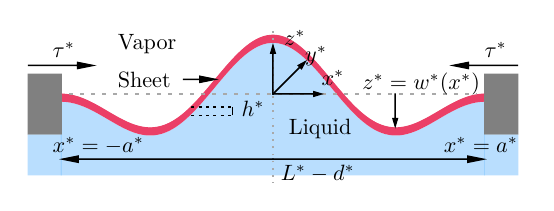
\begin{tikzpicture}

\definecolor{darkgray}{RGB}{169,169,169}
\definecolor{darkgray176}{RGB}{176,176,176}
\definecolor{gray}{RGB}{128,128,128}
\definecolor{indianred23563103}{RGB}{235,63,103}
\definecolor{lightskyblue138200253}{RGB}{138,200,253}

\begin{axis}[
axis equal image,
hide x axis,
hide y axis,
tick align=outside,
tick pos=left,
x grid style={darkgray176},
xlabel={0},
xmin=-0.03311, xmax=0.03311,
xtick style={color=black},
y grid style={darkgray176},
ymin=-0.010863663529839, ymax=0.00813693412661942,
ytick style={color=black}
]
\path [fill=lightskyblue138200253, fill opacity=0.6]
(axis cs:-0.0260467875630729,-0.00095)
--(axis cs:-0.0260467875630729,-0.00095)
--(axis cs:-0.0259887601975588,-0.000950265193764294)
--(axis cs:-0.0259307328320446,-0.000951060839657842)
--(axis cs:-0.0258727054665305,-0.000952386935837379)
--(axis cs:-0.0258146781010164,-0.000954243348798273)
--(axis cs:-0.0257566507355023,-0.000956629813394401)
--(axis cs:-0.0256986233699882,-0.000959545932885385)
--(axis cs:-0.0256405960044741,-0.0009629911790112)
--(axis cs:-0.02558256863896,-0.0009669648920941)
--(axis cs:-0.0255245412734459,-0.0009714662811679)
--(axis cs:-0.0254665139079318,-0.0009764944241347)
--(axis cs:-0.0254084865424177,-0.0009820482679484)
--(axis cs:-0.0253504591769036,-0.0009881266288259)
--(axis cs:-0.0252924318113895,-0.0009947281924857)
--(axis cs:-0.0252344044458754,-0.0010018515144127)
--(axis cs:-0.0251763770803613,-0.0010094950201512)
--(axis cs:-0.0251183497148472,-0.0010176570056243)
--(axis cs:-0.0250603223493331,-0.00102633563748)
--(axis cs:-0.025002294983819,-0.0010355289534653)
--(axis cs:-0.0249442676183049,-0.001045234862826)
--(axis cs:-0.0248862402527908,-0.0010554511467335)
--(axis cs:-0.0248282128872767,-0.0010661754587388)
--(axis cs:-0.0247701855217626,-0.0010774053252526)
--(axis cs:-0.0247121581562485,-0.0010891381460517)
--(axis cs:-0.0246541307907344,-0.0011013711948125)
--(axis cs:-0.0245961034252203,-0.00111410161967)
--(axis cs:-0.0245380760597062,-0.0011273264438032)
--(axis cs:-0.0244800486941921,-0.0011410425660469)
--(axis cs:-0.024422021328678,-0.001155246761529)
--(axis cs:-0.0243639939631638,-0.0011699356823334)
--(axis cs:-0.0243059665976497,-0.0011851058581895)
--(axis cs:-0.0242479392321356,-0.0012007536971861)
--(axis cs:-0.0241899118666215,-0.0012168754865111)
--(axis cs:-0.0241318845011074,-0.0012334673932171)
--(axis cs:-0.0240738571355933,-0.0012505254650108)
--(axis cs:-0.0240158297700792,-0.0012680456310682)
--(axis cs:-0.0239578024045651,-0.0012860237028747)
--(axis cs:-0.023899775039051,-0.0013044553750889)
--(axis cs:-0.0238417476735369,-0.0013233362264317)
--(axis cs:-0.0237837203080228,-0.0013426617205992)
--(axis cs:-0.0237256929425087,-0.0013624272071996)
--(axis cs:-0.0236676655769946,-0.0013826279227144)
--(axis cs:-0.0236096382114805,-0.0014032589914829)
--(axis cs:-0.0235516108459664,-0.00142431542671)
--(axis cs:-0.0234935834804523,-0.0014457921314979)
--(axis cs:-0.0234355561149382,-0.0014676838999004)
--(axis cs:-0.0233775287494241,-0.0014899854180001)
--(axis cs:-0.02331950138391,-0.0015126912650084)
--(axis cs:-0.0232614740183959,-0.001535795914388)
--(axis cs:-0.0232034466528818,-0.0015592937349971)
--(axis cs:-0.0231454192873677,-0.0015831789922564)
--(axis cs:-0.0230873919218536,-0.0016074458493369)
--(axis cs:-0.0230293645563395,-0.0016320883683701)
--(axis cs:-0.0229713371908254,-0.0016571005116786)
--(axis cs:-0.0229133098253113,-0.0016824761430286)
--(axis cs:-0.0228552824597972,-0.0017082090289024)
--(axis cs:-0.022797255094283,-0.0017342928397919)
--(axis cs:-0.0227392277287689,-0.0017607211515122)
--(axis cs:-0.0226812003632548,-0.0017874874465348)
--(axis cs:-0.0226231729977407,-0.0018145851153413)
--(axis cs:-0.0225651456322266,-0.0018420074577962)
--(axis cs:-0.0225071182667125,-0.0018697476845382)
--(axis cs:-0.0224490909011984,-0.0018977989183919)
--(axis cs:-0.0223910635356843,-0.0019261541957963)
--(axis cs:-0.0223330361701702,-0.0019548064682534)
--(axis cs:-0.0222750088046561,-0.0019837486037933)
--(axis cs:-0.022216981439142,-0.0020129733884583)
--(axis cs:-0.0221589540736279,-0.0020424735278035)
--(axis cs:-0.0221009267081138,-0.0020722416484151)
--(axis cs:-0.0220428993425997,-0.0021022702994453)
--(axis cs:-0.0219848719770856,-0.0021325519541642)
--(axis cs:-0.0219268446115715,-0.0021630790115269)
--(axis cs:-0.0218688172460574,-0.0021938437977579)
--(axis cs:-0.0218107898805433,-0.0022248385679495)
--(axis cs:-0.0217527625150292,-0.0022560555076774)
--(axis cs:-0.0216947351495151,-0.0022874867346291)
--(axis cs:-0.021636707784001,-0.002319124300249)
--(axis cs:-0.0215786804184869,-0.0023509601913962)
--(axis cs:-0.0215206530529728,-0.0023829863320169)
--(axis cs:-0.0214626256874587,-0.0024151945848308)
--(axis cs:-0.0214045983219446,-0.0024475767530302)
--(axis cs:-0.0213465709564305,-0.002480124581992)
--(axis cs:-0.0212885435909164,-0.0025128297610032)
--(axis cs:-0.0212305162254023,-0.0025456839249973)
--(axis cs:-0.0211724888598882,-0.002578678656304)
--(axis cs:-0.021114461494374,-0.0026118054864094)
--(axis cs:-0.0210564341288599,-0.0026450558977279)
--(axis cs:-0.0209984067633458,-0.0026784213253852)
--(axis cs:-0.0209403793978317,-0.002711893159011)
--(axis cs:-0.0208823520323176,-0.0027454627445428)
--(axis cs:-0.0208243246668035,-0.0027791213860387)
--(axis cs:-0.0207662973012894,-0.0028128603475)
--(axis cs:-0.0207082699357753,-0.0028466708547028)
--(axis cs:-0.0206502425702612,-0.0028805440970383)
--(axis cs:-0.0205922152047471,-0.0029144712293615)
--(axis cs:-0.020534187839233,-0.0029484433738474)
--(axis cs:-0.0204761604737189,-0.0029824516218552)
--(axis cs:-0.0204181331082048,-0.0030164870357999)
--(axis cs:-0.0203601057426907,-0.0030505406510301)
--(axis cs:-0.0203020783771766,-0.0030846034777124)
--(axis cs:-0.0202440510116625,-0.0031186665027225)
--(axis cs:-0.0201860236461484,-0.0031527206915414)
--(axis cs:-0.0201279962806343,-0.0031867569901566)
--(axis cs:-0.0200699689151202,-0.0032207663269691)
--(axis cs:-0.0200119415496061,-0.0032547396147045)
--(axis cs:-0.019953914184092,-0.0032886677523278)
--(axis cs:-0.0198958868185779,-0.0033225416269632)
--(axis cs:-0.0198378594530638,-0.0033563521158155)
--(axis cs:-0.0197798320875497,-0.0033900900880965)
--(axis cs:-0.0197218047220356,-0.0034237464069524)
--(axis cs:-0.0196637773565215,-0.0034573119313946)
--(axis cs:-0.0196057499910074,-0.0034907775182313)
--(axis cs:-0.0195477226254933,-0.0035241340240011)
--(axis cs:-0.0194896952599792,-0.0035573723069084)
--(axis cs:-0.019431667894465,-0.0035904832287575)
--(axis cs:-0.0193736405289509,-0.0036234576568893)
--(axis cs:-0.0193156131634368,-0.0036562864661163)
--(axis cs:-0.0192575857979227,-0.0036889605406574)
--(axis cs:-0.0191995584324086,-0.0037214707760725)
--(axis cs:-0.0191415310668945,-0.0037538080811952)
--(axis cs:-0.0190835037013804,-0.003785963380064)
--(axis cs:-0.0190254763358663,-0.0038179276138512)
--(axis cs:-0.0189674489703522,-0.0038496917427901)
--(axis cs:-0.0189094216048381,-0.0038812467480988)
--(axis cs:-0.018851394239324,-0.0039125836339006)
--(axis cs:-0.0187933668738099,-0.0039436934291412)
--(axis cs:-0.0187353395082958,-0.0039745671895024)
--(axis cs:-0.0186773121427817,-0.0040051959993101)
--(axis cs:-0.0186192847772676,-0.0040355709734386)
--(axis cs:-0.0185612574117535,-0.0040656832592097)
--(axis cs:-0.0185032300462394,-0.0040955240382859)
--(axis cs:-0.0184452026807253,-0.0041250845285578)
--(axis cs:-0.0183871753152112,-0.0041543559860256)
--(axis cs:-0.0183291479496971,-0.004183329706673)
--(axis cs:-0.018271120584183,-0.0042119970283357)
--(axis cs:-0.0182130932186689,-0.0042403493325605)
--(axis cs:-0.0181550658531548,-0.0042683780464584)
--(axis cs:-0.0180970384876407,-0.0042960746445482)
--(axis cs:-0.0180390111221266,-0.0043234306505924)
--(axis cs:-0.0179809837566125,-0.0043504376394242)
--(axis cs:-0.0179229563910984,-0.0043770872387641)
--(axis cs:-0.0178649290255843,-0.0044033711310288)
--(axis cs:-0.0178069016600702,-0.0044292810551283)
--(axis cs:-0.0177488742945561,-0.0044548088082534)
--(axis cs:-0.0176908469290419,-0.0044799462476529)
--(axis cs:-0.0176328195635278,-0.0045046852923988)
--(axis cs:-0.0175747921980137,-0.0045290179251406)
--(axis cs:-0.0175167648324996,-0.0045529361938479)
--(axis cs:-0.0174587374669855,-0.0045764322135405)
--(axis cs:-0.0174007101014714,-0.0045994981680062)
--(axis cs:-0.0173426827359573,-0.0046221263115058)
--(axis cs:-0.0172846553704432,-0.0046443089704646)
--(axis cs:-0.0172266280049291,-0.004666038545151)
--(axis cs:-0.017168600639415,-0.0046873075113404)
--(axis cs:-0.0171105732739009,-0.0047081084219658)
--(axis cs:-0.0170525459083868,-0.0047284339087529)
--(axis cs:-0.0169945185428727,-0.004748276683841)
--(axis cs:-0.0169364911773586,-0.0047676295413887)
--(axis cs:-0.0168784638118445,-0.0047864853591634)
--(axis cs:-0.0168204364463304,-0.004804837100116)
--(axis cs:-0.0167624090808163,-0.0048226778139384)
--(axis cs:-0.0167043817153022,-0.0048400006386051)
--(axis cs:-0.0166463543497881,-0.004856798801898)
--(axis cs:-0.016588326984274,-0.0048730656229136)
--(axis cs:-0.0165302996187599,-0.0048887945135536)
--(axis cs:-0.0164722722532458,-0.0049039789799969)
--(axis cs:-0.0164142448877317,-0.0049186126241543)
--(axis cs:-0.0163562175222176,-0.0049326891451044)
--(axis cs:-0.0162981901567035,-0.004946202340511)
--(axis cs:-0.0162401627911894,-0.0049591461080219)
--(axis cs:-0.0161821354256753,-0.0049715144466483)
--(axis cs:-0.0161241080601612,-0.0049833014581245)
--(axis cs:-0.016066080694647,-0.0049945013482481)
--(axis cs:-0.0160080533291329,-0.0050051084282006)
--(axis cs:-0.0159500259636188,-0.0050151171158466)
--(axis cs:-0.0158919985981047,-0.0050245219370138)
--(axis cs:-0.0158339712325906,-0.0050333175267513)
--(axis cs:-0.0157759438670765,-0.0050414986305666)
--(axis cs:-0.0157179165015624,-0.0050490601056428)
--(axis cs:-0.0156598891360483,-0.0050559969220319)
--(axis cs:-0.0156018617705342,-0.0050623041638287)
--(axis cs:-0.0155438344050201,-0.0050679770303207)
--(axis cs:-0.015485807039506,-0.0050730108371168)
--(axis cs:-0.0154277796739919,-0.0050774010172532)
--(axis cs:-0.0153697523084778,-0.0050811431222766)
--(axis cs:-0.0153117249429637,-0.005084232823304)
--(axis cs:-0.0152536975774496,-0.0050866659120601)
--(axis cs:-0.0151956702119355,-0.0050884383018905)
--(axis cs:-0.0151376428464214,-0.0050895460287518)
--(axis cs:-0.0150796154809073,-0.0050899852521776)
--(axis cs:-0.0150215881153932,-0.0050897522562207)
--(axis cs:-0.0149635607498791,-0.0050888434503707)
--(axis cs:-0.014905533384365,-0.005087255370448)
--(axis cs:-0.0148475060188509,-0.0050849846794718)
--(axis cs:-0.0147894786533368,-0.0050820281685051)
--(axis cs:-0.0147314512878227,-0.005078382757473)
--(axis cs:-0.0146734239223086,-0.0050740454959573)
--(axis cs:-0.0146153965567945,-0.005069013563965)
--(axis cs:-0.0145573691912804,-0.0050632842726713)
--(axis cs:-0.0144993418257662,-0.0050568550651379)
--(axis cs:-0.0144413144602522,-0.0050497235170041)
--(axis cs:-0.014383287094738,-0.0050418873371532)
--(axis cs:-0.0143252597292239,-0.0050333443683527)
--(axis cs:-0.0142672323637098,-0.0050240925878675)
--(axis cs:-0.0142092049981957,-0.0050141301080476)
--(axis cs:-0.0141511776326816,-0.0050034551768892)
--(axis cs:-0.0140931502671675,-0.0049920661785691)
--(axis cs:-0.0140351229016534,-0.0049799616339523)
--(axis cs:-0.0139770955361393,-0.0049671402010732)
--(axis cs:-0.0139190681706252,-0.0049536006755896)
--(axis cs:-0.0138610408051111,-0.0049393419912099)
--(axis cs:-0.013803013439597,-0.0049243632200929)
--(axis cs:-0.0137449860740829,-0.004908663573221)
--(axis cs:-0.0136869587085688,-0.0048922424007455)
--(axis cs:-0.0136289313430547,-0.0048750991923051)
--(axis cs:-0.0135709039775406,-0.0048572335773168)
--(axis cs:-0.0135128766120265,-0.0048386453252388)
--(axis cs:-0.0134548492465124,-0.0048193343458073)
--(axis cs:-0.0133968218809983,-0.0047993006892437)
--(axis cs:-0.0133387945154842,-0.0047785445464361)
--(axis cs:-0.0132807671499701,-0.004757066249092)
--(axis cs:-0.013222739784456,-0.0047348662698632)
--(axis cs:-0.0131647124189419,-0.0047119452224437)
--(axis cs:-0.0131066850534278,-0.0046883038616392)
--(axis cs:-0.0130486576879137,-0.0046639430834091)
--(axis cs:-0.0129906303223996,-0.0046388639248803)
--(axis cs:-0.0129326029568855,-0.0046130675643335)
--(axis cs:-0.0128745755913714,-0.0045865553211618)
--(axis cs:-0.0128165482258572,-0.0045593286558008)
--(axis cs:-0.0127585208603431,-0.0045313891696316)
--(axis cs:-0.012700493494829,-0.0045027386048555)
--(axis cs:-0.0126424661293149,-0.0044733788443407)
--(axis cs:-0.0125844387638008,-0.0044433119114421)
--(axis cs:-0.0125264113982867,-0.0044125399697922)
--(axis cs:-0.0124683840327726,-0.004381065323065)
--(axis cs:-0.0124103566672585,-0.0043488904147121)
--(axis cs:-0.0123523293017444,-0.0043160178276705)
--(axis cs:-0.0122943019362303,-0.0042824502840439)
--(axis cs:-0.0122362745707162,-0.0042481906447556)
--(axis cs:-0.0121782472052021,-0.0042132419091739)
--(axis cs:-0.012120219839688,-0.0041776072147107)
--(axis cs:-0.0120621924741739,-0.0041412898363918)
--(axis cs:-0.0120041651086598,-0.0041042931864011)
--(axis cs:-0.0119461377431457,-0.0040666208135963)
--(axis cs:-0.0118881103776316,-0.0040282764029982)
--(axis cs:-0.0118300830121175,-0.0039892637752531)
--(axis cs:-0.0117720556466034,-0.0039495868860678)
--(axis cs:-0.0117140282810893,-0.0039092498256181)
--(axis cs:-0.0116560009155752,-0.0038682568179303)
--(axis cs:-0.0115979735500611,-0.0038266122202361)
--(axis cs:-0.011539946184547,-0.0037843205223014)
--(axis cs:-0.0114819188190329,-0.0037413863457285)
--(axis cs:-0.0114238914535188,-0.0036978144432314)
--(axis cs:-0.0113658640880047,-0.0036536096978864)
--(axis cs:-0.0113078367224906,-0.003608777122355)
--(axis cs:-0.0112498093569765,-0.0035633218580827)
--(axis cs:-0.0111917819914624,-0.0035172491744708)
--(axis cs:-0.0111337546259482,-0.0034705644680232)
--(axis cs:-0.0110757272604341,-0.0034232732614678)
--(axis cs:-0.01101769989492,-0.0033753812028528)
--(axis cs:-0.0109596725294059,-0.0033268940646176)
--(axis cs:-0.0109016451638918,-0.0032778177426395)
--(axis cs:-0.0108436177983777,-0.0032281582552545)
--(axis cs:-0.0107855904328636,-0.0031779217422552)
--(axis cs:-0.0107275630673495,-0.0031271144638632)
--(axis cs:-0.0106695357018354,-0.0030757427996777)
--(axis cs:-0.0106115083363213,-0.0030238132476002)
--(axis cs:-0.0105534809708072,-0.002971332422736)
--(axis cs:-0.0104954536052931,-0.0029183070562708)
--(axis cs:-0.010437426239779,-0.0028647439943259)
--(axis cs:-0.0103793988742649,-0.0028106501967886)
--(axis cs:-0.0103213715087508,-0.0027560327361208)
--(axis cs:-0.0102633441432367,-0.0027008987961445)
--(axis cs:-0.0102053167777226,-0.0026452556708052)
--(axis cs:-0.0101472894122085,-0.0025891107629128)
--(axis cs:-0.0100892620466944,-0.0025324715828607)
--(axis cs:-0.0100312346811803,-0.0024753457473236)
--(axis cs:-0.0099732073156662,-0.002417740977933)
--(axis cs:-0.0099151799501521,-0.0023596650999325)
--(axis cs:-0.009857152584638,-0.0023011260408115)
--(axis cs:-0.0097991252191239,-0.0022421318289185)
--(axis cs:-0.0097410978536098,-0.0021826905920538)
--(axis cs:-0.0096830704880957,-0.0021228105560424)
--(axis cs:-0.0096250431225816,-0.002062500043287)
--(axis cs:-0.0095670157570675,-0.0020017674713008)
--(axis cs:-0.0095089883915534,-0.001940621351222)
--(axis cs:-0.0094509610260392,-0.0018790702863083)
--(axis cs:-0.0093929336605251,-0.0018171229704134)
--(axis cs:-0.009334906295011,-0.001754788186445)
--(axis cs:-0.0092768789294969,-0.0016920748048038)
--(axis cs:-0.0092188515639828,-0.0016289917818061)
--(axis cs:-0.0091608241984687,-0.0015655481580875)
--(axis cs:-0.0091027968329546,-0.0015017530569903)
--(axis cs:-0.0090447694674405,-0.0014376156829333)
--(axis cs:-0.0089867421019264,-0.0013731453197656)
--(axis cs:-0.0089287147364123,-0.0013083513291039)
--(axis cs:-0.0088706873708982,-0.0012432431486535)
--(axis cs:-0.0088126600053841,-0.0011778302905138)
--(axis cs:-0.00875463263987,-0.0011121223394691)
--(axis cs:-0.0086966052743559,-0.0010461289512635)
--(axis cs:-0.0086385779088418,-0.0009798598508618)
--(axis cs:-0.0085805505433277,-0.0009133248306954)
--(axis cs:-0.0085225231778136,-0.0008465337488949)
--(axis cs:-0.0084644958122995,-0.000779496527509)
--(axis cs:-0.0084064684467854,-0.0007122231507094)
--(axis cs:-0.0083484410812713,-0.0006447236629836)
--(axis cs:-0.0082904137157572,-0.0005770081673146)
--(axis cs:-0.0082323863502431,-0.0005090868233482)
--(axis cs:-0.008174358984729,-0.000440969845549)
--(axis cs:-0.0081163316192149,-0.0003726675013445)
--(axis cs:-0.0080583042537008,-0.0003041901092578)
--(axis cs:-0.0080002768881867,-0.0002355480370296)
--(axis cs:-0.0079422495226726,-0.0001667516997302)
--(axis cs:-0.0078842221571585,-9.78115578609e-05)
--(axis cs:-0.0078261947916443,-2.87381154455e-05)
--(axis cs:-0.0077681674261302,4.04580818869001e-05)
--(axis cs:-0.0077101400606161,0.0001097664488288)
--(axis cs:-0.007652112695102,0.000179176362329)
--(axis cs:-0.0075940853295879,0.0002486771635367)
--(axis cs:-0.0075360579640738,0.0003182581597521)
--(axis cs:-0.0074780305985597,0.0003879086263859)
--(axis cs:-0.0074200032330456,0.0004576178089245)
--(axis cs:-0.0073619758675315,0.0005273749249031)
--(axis cs:-0.0073039485020174,0.0005971691658846)
--(axis cs:-0.0072459211365033,0.0006669896994445)
--(axis cs:-0.0071878937709892,0.0007368256711616)
--(axis cs:-0.0071298664054751,0.0008066662066133)
--(axis cs:-0.007071839039961,0.0008765004133766)
--(axis cs:-0.0070138116744469,0.000946317383033)
--(axis cs:-0.0069557843089328,0.0010161061931771)
--(axis cs:-0.0068977569434187,0.0010858559094298)
--(axis cs:-0.0068397295779046,0.0011555555874539)
--(axis cs:-0.0067817022123905,0.0012251942749728)
--(axis cs:-0.0067236748468764,0.0012947610137919)
--(axis cs:-0.0066656474813623,0.0013642448418217)
--(axis cs:-0.0066076201158482,0.001433634795103)
--(axis cs:-0.0065495927503341,0.0015029199098332)
--(axis cs:-0.00649156538482,0.0015720892243932)
--(axis cs:-0.0064335380193059,0.0016411317813754)
--(axis cs:-0.0063755106537918,0.0017100366296114)
--(axis cs:-0.0063174832882777,0.0017787928261994)
--(axis cs:-0.0062594559227636,0.0018473894385313)
--(axis cs:-0.0062014285572495,0.0019158155463182)
--(axis cs:-0.0061434011917353,0.0019840602436151)
--(axis cs:-0.0060853738262212,0.0020521126408427)
--(axis cs:-0.0060273464607071,0.0021199618668086)
--(axis cs:-0.005969319095193,0.0021875970707238)
--(axis cs:-0.0059112917296789,0.002255007424218)
--(axis cs:-0.0058532643641648,0.0023221821233506)
--(axis cs:-0.0057952369986507,0.0023891103906177)
--(axis cs:-0.0057372096331366,0.0024557814769555)
--(axis cs:-0.0056791822676225,0.0025221846637386)
--(axis cs:-0.0056211549021084,0.0025883092647736)
--(axis cs:-0.0055631275365943,0.0026541446282875)
--(axis cs:-0.0055051001710802,0.0027196801389097)
--(axis cs:-0.0054470728055661,0.0027849052196483)
--(axis cs:-0.005389045440052,0.0028498093338603)
--(axis cs:-0.0053310180745379,0.0029143819872138)
--(axis cs:-0.0052729907090238,0.0029786127296439)
--(axis cs:-0.0052149633435097,0.0030424911573005)
--(axis cs:-0.0051569359779956,0.0031060069144879)
--(axis cs:-0.0050989086124815,0.0031691496955965)
--(axis cs:-0.0050408812469674,0.0032319092470251)
--(axis cs:-0.0049828538814533,0.0032942753690946)
--(axis cs:-0.0049248265159392,0.0033562379179513)
--(axis cs:-0.0048667991504251,0.0034177868074615)
--(axis cs:-0.004808771784911,0.0034789120110947)
--(axis cs:-0.0047507444193969,0.0035396035637965)
--(axis cs:-0.0046927170538828,0.003599851563851)
--(axis cs:-0.0046346896883687,0.0036596461747309)
--(axis cs:-0.0045766623228546,0.0037189776269367)
--(axis cs:-0.0045186349573404,0.0037778362198231)
--(axis cs:-0.0044606075918263,0.0038362123234136)
--(axis cs:-0.0044025802263122,0.0038940963802016)
--(axis cs:-0.0043445528607981,0.003951478906939)
--(axis cs:-0.004286525495284,0.0040083504964109)
--(axis cs:-0.0042284981297699,0.0040647018191964)
--(axis cs:-0.0041704707642558,0.0041205236254156)
--(axis cs:-0.0041124433987417,0.0041758067464615)
--(axis cs:-0.0040544160332276,0.0042305420967175)
--(axis cs:-0.0039963886677135,0.0042847206752595)
--(axis cs:-0.0039383613021994,0.0043383335675425)
--(axis cs:-0.0038803339366853,0.0043913719470711)
--(axis cs:-0.0038223065711712,0.0044438270770541)
--(axis cs:-0.0037642792056571,0.0044956903120428)
--(axis cs:-0.003706251840143,0.0045469530995516)
--(axis cs:-0.0036482244746289,0.0045976069816624)
--(axis cs:-0.0035901971091148,0.0046476435966109)
--(axis cs:-0.0035321697436007,0.0046970546803555)
--(axis cs:-0.0034741423780866,0.0047458320681279)
--(axis cs:-0.0034161150125725,0.0047939676959654)
--(axis cs:-0.0033580876470584,0.0048414536022244)
--(axis cs:-0.0033000602815443,0.0048882819290753)
--(axis cs:-0.0032420329160302,0.0049344449239776)
--(axis cs:-0.0031840055505161,0.0049799349411358)
--(axis cs:-0.003125978185002,0.0050247444429354)
--(axis cs:-0.0030679508194879,0.0050688660013585)
--(axis cs:-0.0030099234539738,0.0051122922993799)
--(axis cs:-0.0029518960884597,0.0051550161323409)
--(axis cs:-0.0028938687229456,0.0051970304093041)
--(axis cs:-0.0028358413574314,0.0052383281543854)
--(axis cs:-0.0027778139919173,0.0052789025080655)
--(axis cs:-0.0027197866264032,0.0053187467284794)
--(axis cs:-0.0026617592608891,0.0053578541926837)
--(axis cs:-0.002603731895375,0.0053962183979018)
--(axis cs:-0.0025457045298609,0.0054338329627473)
--(axis cs:-0.0024876771643468,0.0054706916284235)
--(axis cs:-0.0024296497988327,0.0055067882599011)
--(axis cs:-0.0023716224333186,0.0055421168470718)
--(axis cs:-0.0023135950678045,0.0055766715058794)
--(axis cs:-0.0022555677022904,0.0056104464794266)
--(axis cs:-0.0021975403367763,0.0056434361390583)
--(axis cs:-0.0021395129712622,0.0056756349854209)
--(axis cs:-0.0020814856057481,0.0057070376494972)
--(axis cs:-0.002023458240234,0.0057376388936169)
--(axis cs:-0.0019654308747199,0.0057674336124427)
--(axis cs:-0.0019074035092058,0.005796416833931)
--(axis cs:-0.0018493761436917,0.0058245837202684)
--(axis cs:-0.0017913487781776,0.0058519295687821)
--(axis cs:-0.0017333214126635,0.0058784498128259)
--(axis cs:-0.0016752940471494,0.0059041400226397)
--(axis cs:-0.0016172666816353,0.0059289959061837)
--(axis cs:-0.0015592393161212,0.0059530133099471)
--(axis cs:-0.0015012119506071,0.0059761882197301)
--(axis cs:-0.001443184585093,0.0059985167614001)
--(axis cs:-0.0013851572195789,0.0060199952016214)
--(axis cs:-0.0013271298540648,0.0060406199485585)
--(axis cs:-0.0012691024885507,0.006060387552553)
--(axis cs:-0.0012110751230365,0.0060792947067731)
--(axis cs:-0.0011530477575224,0.0060973382478368)
--(axis cs:-0.0010950203920083,0.0061145151564082)
--(axis cs:-0.0010369930264942,0.0061308225577661)
--(axis cs:-0.0009789656609801,0.0061462577223458)
--(axis cs:-0.000920938295466,0.0061608180662536)
--(axis cs:-0.0008629109299519,0.0061745011517535)
--(axis cs:-0.0008048835644378,0.0061873046877267)
--(axis cs:-0.0007468561989237,0.0061992265301038)
--(axis cs:-0.0006888288334096,0.0062102646822681)
--(axis cs:-0.0006308014678955,0.0062204172954327)
--(axis cs:-0.0005727741023814,0.0062296826689883)
--(axis cs:-0.0005147467368673,0.0062380592508244)
--(axis cs:-0.0004567193713532,0.0062455456376213)
--(axis cs:-0.0003986920058391,0.0062521405751149)
--(axis cs:-0.000340664640325,0.0062578429583332)
--(axis cs:-0.0002826372748109,0.0062626518318042)
--(axis cs:-0.0002246099092968,0.0062665663897367)
--(axis cs:-0.0001665825437827,0.0062695859761714)
--(axis cs:-0.0001085551782686,0.0062717100851051)
--(axis cs:-5.05278127545e-05,0.0062729383605859)
--(axis cs:7.49955275957484e-06,0.0062732705967804)
--(axis cs:6.55269182736e-05,0.0062727067380123)
--(axis cs:0.0001235542837877,0.0062712468787732)
--(axis cs:0.0001815816493018,0.0062688912637045)
--(axis cs:0.0002396090148159,0.0062656402875514)
--(axis cs:0.00029763638033,0.0062614944950884)
--(axis cs:0.0003556637458441,0.006256454581017)
--(axis cs:0.0004136911113583,0.006250521389834)
--(axis cs:0.0004717184768724,0.0062436959156731)
--(axis cs:0.0005297458423865,0.0062359793021168)
--(axis cs:0.0005877732079006,0.0062273728419815)
--(axis cs:0.0006458005734147,0.0062178779770732)
--(axis cs:0.0007038279389288,0.0062074962979162)
--(axis cs:0.0007618553044429,0.0061962295434529)
--(axis cs:0.000819882669957,0.0061840796007164)
--(axis cs:0.0008779100354711,0.0061710485044744)
--(axis cs:0.0009359374009852,0.0061571384368463)
--(axis cs:0.0009939647664993,0.0061423517268912)
--(axis cs:0.0010519921320134,0.0061266908501698)
--(axis cs:0.0011100194975275,0.0061101584282769)
--(axis cs:0.0011680468630416,0.0060927572283482)
--(axis cs:0.0012260742285557,0.0060744901625383)
--(axis cs:0.0012841015940698,0.0060553602874725)
--(axis cs:0.0013421289595839,0.0060353708036701)
--(axis cs:0.001400156325098,0.0060145250549421)
--(axis cs:0.0014581836906121,0.0059928265277606)
--(axis cs:0.0015162110561262,0.0059702788506027)
--(axis cs:0.0015742384216403,0.0059468857932659)
--(axis cs:0.0016322657871544,0.005922651266159)
--(axis cs:0.0016902931526685,0.0058975793195649)
--(axis cs:0.0017483205181826,0.0058716741428779)
--(axis cs:0.0018063478836967,0.0058449400638145)
--(axis cs:0.0018643752492108,0.0058173815475987)
--(axis cs:0.0019224026147249,0.0057890031961207)
--(axis cs:0.001980429980239,0.0057598097470708)
--(axis cs:0.0020384573457531,0.005729806073047)
--(axis cs:0.0020964847112673,0.0056989971806378)
--(axis cs:0.0021545120767814,0.0056673882094794)
--(axis cs:0.0022125394422955,0.0056349844312886)
--(axis cs:0.0022705668078096,0.0056017912488703)
--(axis cs:0.0023285941733237,0.0055678141951005)
--(axis cs:0.0023866215388378,0.0055330589318852)
--(axis cs:0.0024446489043519,0.0054975312490949)
--(axis cs:0.002502676269866,0.0054612370634753)
--(axis cs:0.0025607036353801,0.005424182417534)
--(axis cs:0.0026187310008942,0.0053863734784036)
--(axis cs:0.0026767583664083,0.0053478165366819)
--(axis cs:0.0027347857319224,0.0053085180052486)
--(axis cs:0.0027928130974365,0.0052684844180596)
--(axis cs:0.0028508404629506,0.0052277224289176)
--(axis cs:0.0029088678284647,0.0051862388102218)
--(axis cs:0.0029668951939788,0.0051440404516942)
--(axis cs:0.0030249225594929,0.0051011343590849)
--(axis cs:0.003082949925007,0.0050575276528549)
--(axis cs:0.0031409772905211,0.0050132275668382)
--(axis cs:0.0031990046560352,0.0049682414468826)
--(axis cs:0.0032570320215493,0.0049225767494693)
--(axis cs:0.0033150593870634,0.0048762410403122)
--(axis cs:0.0033730867525775,0.0048292419929372)
--(axis cs:0.0034311141180916,0.0047815873872405)
--(axis cs:0.0034891414836057,0.004733285108028)
--(axis cs:0.0035471688491198,0.0046843431435352)
--(axis cs:0.0036051962146339,0.0046347695839272)
--(axis cs:0.003663223580148,0.0045845726197802)
--(axis cs:0.0037212509456621,0.004533760540545)
--(axis cs:0.0037792783111762,0.004482341732991)
--(axis cs:0.0038373056766904,0.0044303246796332)
--(axis cs:0.0038953330422045,0.0043777179571411)
--(axis cs:0.0039533604077186,0.0043245302347299)
--(axis cs:0.0040113877732327,0.0042707702725355)
--(axis cs:0.0040694151387468,0.0042164469199718)
--(axis cs:0.0041274425042609,0.0041615691140721)
--(axis cs:0.004185469869775,0.0041061458778145)
--(axis cs:0.0042434972352891,0.0040501863184309)
--(axis cs:0.0043015246008032,0.0039936996257012)
--(axis cs:0.0043595519663173,0.0039366950702318)
--(axis cs:0.0044175793318314,0.0038791820017202)
--(axis cs:0.0044756066973455,0.0038211698472038)
--(axis cs:0.0045336340628596,0.003762668109296)
--(axis cs:0.0045916614283737,0.0037036863644075)
--(axis cs:0.0046496887938878,0.0036442342609547)
--(axis cs:0.0047077161594019,0.0035843215175549)
--(axis cs:0.004765743524916,0.0035239579212088)
--(axis cs:0.0048237708904301,0.0034631533254706)
--(axis cs:0.0048817982559442,0.0034019176486059)
--(axis cs:0.0049398256214583,0.0033402608717384)
--(axis cs:0.0049978529869724,0.0032781930369852)
--(axis cs:0.0050558803524865,0.0032157242455805)
--(axis cs:0.0051139077180006,0.0031528646559898)
--(axis cs:0.0051719350835147,0.003089624482013)
--(axis cs:0.0052299624490288,0.0030260139908785)
--(axis cs:0.0052879898145429,0.0029620435013268)
--(axis cs:0.005346017180057,0.0028977233816861)
--(axis cs:0.0054040445455711,0.0028330640479385)
--(axis cs:0.0054620719110853,0.0027680759617783)
--(axis cs:0.0055200992765994,0.0027027696286617)
--(axis cs:0.0055781266421135,0.0026371555958498)
--(axis cs:0.0056361540076276,0.0025712444504435)
--(axis cs:0.0056941813731417,0.0025050468174126)
--(axis cs:0.0057522087386558,0.0024385733576175)
--(axis cs:0.0058102361041699,0.0023718347658253)
--(axis cs:0.005868263469684,0.0023048417687207)
--(axis cs:0.0059262908351981,0.0022376051229103)
--(axis cs:0.0059843182007122,0.0021701356129237)
--(axis cs:0.0060423455662263,0.0021024440492087)
--(axis cs:0.0061003729317404,0.0020345412661233)
--(axis cs:0.0061584002972545,0.0019664381199237)
--(axis cs:0.0062164276627686,0.0018981454867484)
--(axis cs:0.0062744550282827,0.0018296742606007)
--(axis cs:0.0063324823937968,0.0017610353513271)
--(axis cs:0.0063905097593109,0.001692239682595)
--(axis cs:0.006448537124825,0.0016232981898673)
--(axis cs:0.0065065644903391,0.001554221818377)
--(axis cs:0.0065645918558532,0.0014850215210994)
--(axis cs:0.0066226192213673,0.0014157082567252)
--(axis cs:0.0066806465868814,0.001346292987632)
--(axis cs:0.0067386739523955,0.0012767866778573)
--(axis cs:0.0067967013179096,0.0012072002910712)
--(axis cs:0.0068547286834237,0.0011375447885503)
--(axis cs:0.0069127560489378,0.0010678311271533)
--(axis cs:0.0069707834144519,0.0009980702572983)
--(axis cs:0.007028810779966,0.0009282731209418)
--(axis cs:0.0070868381454802,0.0008584506495611)
--(axis cs:0.0071448655109943,0.0007886137621388)
--(axis cs:0.0072028928765084,0.0007187733631513)
--(axis cs:0.0072609202420225,0.0006489403405607)
--(axis cs:0.0073189476075366,0.0005791255638111)
--(axis cs:0.0073769749730507,0.000509339881829)
--(axis cs:0.0074350023385648,0.0004395941210292)
--(axis cs:0.0074930297040789,0.0003698990833254)
--(axis cs:0.007551057069593,0.0003002655441467)
--(axis cs:0.0076090844351071,0.0002307042504607)
--(axis cs:0.0076671118006212,0.0001612259188018)
--(axis cs:0.0077251391661353,9.1841233308e-05)
--(axis cs:0.0077831665316494,2.2560843763e-05)
--(axis cs:0.0078411938971635,-4.6604636352e-05)
--(axis cs:0.0078992212626776,-0.0001156446318008)
--(axis cs:0.0079572486281917,-0.0001845486075241)
--(axis cs:0.0080152759937058,-0.0002533060705646)
--(axis cs:0.0080733033592199,-0.0003219065719818)
--(axis cs:0.008131330724734,-0.0003903397087577)
--(axis cs:0.0081893580902481,-0.0004585951256928)
--(axis cs:0.0082473854557622,-0.0005266625172919)
--(axis cs:0.0083054128212763,-0.0005945316296392)
--(axis cs:0.0083634401867904,-0.0006621922622624)
--(axis cs:0.0084214675523045,-0.0007296342699856)
--(axis cs:0.0084794949178186,-0.000796847564771)
--(axis cs:0.0085375222833327,-0.0008638221175477)
--(axis cs:0.0085955496488468,-0.0009305479600291)
--(axis cs:0.0086535770143609,-0.0009970151865167)
--(axis cs:0.0087116043798751,-0.001063213955692)
--(axis cs:0.0087696317453892,-0.0011291344923936)
--(axis cs:0.0088276591109033,-0.0011947670893817)
--(axis cs:0.0088856864764174,-0.001260102109088)
--(axis cs:0.0089437138419315,-0.0013251299853514)
--(axis cs:0.0090017412074456,-0.0013898412251388)
--(axis cs:0.0090597685729597,-0.0014542264102508)
--(axis cs:0.0091177959384738,-0.0015182761990121)
--(axis cs:0.0091758233039879,-0.0015819813279464)
--(axis cs:0.009233850669502,-0.0016453326134344)
--(axis cs:0.0092918780350161,-0.0017083209533569)
--(axis cs:0.0093499054005302,-0.0017709373287194)
--(axis cs:0.0094079327660443,-0.0018331728052611)
--(axis cs:0.0094659601315584,-0.0018950185350463)
--(axis cs:0.0095239874970725,-0.0019564657580374)
--(axis cs:0.0095820148625866,-0.0020175058036514)
--(axis cs:0.0096400422281007,-0.0020781300922963)
--(axis cs:0.0096980695936148,-0.0021383301368913)
--(axis cs:0.0097560969591289,-0.0021980975443657)
--(axis cs:0.009814124324643,-0.002257424017141)
--(axis cs:0.0098721516901571,-0.0023163013545921)
--(axis cs:0.0099301790556712,-0.0023747214544891)
--(axis cs:0.0099882064211853,-0.0024326763144199)
--(axis cs:0.0100462337866994,-0.002490158033192)
--(axis cs:0.0101042611522135,-0.0025471588122137)
--(axis cs:0.0101622885177276,-0.0026036709568549)
--(axis cs:0.0102203158832417,-0.0026596868777869)
--(axis cs:0.0102783432487558,-0.0027151990923009)
--(axis cs:0.01033637061427,-0.0027702002256047)
--(axis cs:0.0103943979797841,-0.0028246830120981)
--(axis cs:0.0104524253452982,-0.0028786402966263)
--(axis cs:0.0105104527108123,-0.0029320650357105)
--(axis cs:0.0105684800763264,-0.0029849502987567)
--(axis cs:0.0106265074418405,-0.0030372892692415)
--(axis cs:0.0106845348073546,-0.0030890752458751)
--(axis cs:0.0107425621728687,-0.0031403016437409)
--(axis cs:0.0108005895383828,-0.0031909619954122)
--(axis cs:0.0108586169038969,-0.0032410499520447)
--(axis cs:0.010916644269411,-0.003290559284446)
--(axis cs:0.0109746716349251,-0.0033394838841205)
--(axis cs:0.0110326990004392,-0.0033878177642905)
--(axis cs:0.0110907263659533,-0.0034355550608927)
--(axis cs:0.0111487537314674,-0.0034826900335504)
--(axis cs:0.0112067810969815,-0.0035292170665205)
--(axis cs:0.0112648084624956,-0.0035751306696162)
--(axis cs:0.0113228358280097,-0.0036204254791044)
--(axis cs:0.0113808631935238,-0.0036650962585775)
--(axis cs:0.0114388905590379,-0.0037091378998003)
--(axis cs:0.011496917924552,-0.0037525454235308)
--(axis cs:0.0115549452900661,-0.0037953139803162)
--(axis cs:0.0116129726555802,-0.0038374388512615)
--(axis cs:0.0116710000210943,-0.0038789154487739)
--(axis cs:0.0117290273866084,-0.0039197393172793)
--(axis cs:0.0117870547521225,-0.0039599061339142)
--(axis cs:0.0118450821176366,-0.0039994117091896)
--(axis cs:0.0119031094831507,-0.0040382519876296)
--(axis cs:0.0119611368486648,-0.0040764230483826)
--(axis cs:0.012019164214179,-0.0041139211058063)
--(axis cs:0.0120771915796931,-0.0041507425100251)
--(axis cs:0.0121352189452072,-0.0041868837474614)
--(axis cs:0.0121932463107213,-0.0042223414413392)
--(axis cs:0.0122512736762354,-0.004257112352161)
--(axis cs:0.0123093010417495,-0.0042911933781567)
--(axis cs:0.0123673284072636,-0.0043245815557064)
--(axis cs:0.0124253557727777,-0.0043572740597346)
--(axis cs:0.0124833831382918,-0.0043892682040776)
--(axis cs:0.0125414105038059,-0.0044205614418237)
--(axis cs:0.01259943786932,-0.0044511513656245)
--(axis cs:0.0126574652348341,-0.0044810357079803)
--(axis cs:0.0127154926003482,-0.0045102123414964)
--(axis cs:0.0127735199658623,-0.0045386792791127)
--(axis cs:0.0128315473313764,-0.0045664346743046)
--(axis cs:0.0128895746968905,-0.0045934768212569)
--(axis cs:0.0129476020624046,-0.0046198041550099)
--(axis cs:0.0130056294279187,-0.0046454152515768)
--(axis cs:0.0130636567934328,-0.0046703088280343)
--(axis cs:0.0131216841589469,-0.0046944837425845)
--(axis cs:0.013179711524461,-0.0047179389945898)
--(axis cs:0.0132377388899751,-0.0047406737245792)
--(axis cs:0.0132957662554892,-0.0047626872142272)
--(axis cs:0.0133537936210033,-0.0047839788863046)
--(axis cs:0.0134118209865174,-0.0048045483046017)
--(axis cs:0.0134698483520315,-0.0048243951738238)
--(axis cs:0.0135278757175456,-0.0048435193394584)
--(axis cs:0.0135859030830597,-0.0048619207876156)
--(axis cs:0.0136439304485738,-0.0048795996448399)
--(axis cs:0.013701957814088,-0.004896556177895)
--(axis cs:0.0137599851796021,-0.0049127907935207)
--(axis cs:0.0138180125451162,-0.0049283040381624)
--(axis cs:0.0138760399106303,-0.0049430965976733)
--(axis cs:0.0139340672761444,-0.0049571692969887)
--(axis cs:0.0139920946416585,-0.0049705230997738)
--(axis cs:0.0140501220071726,-0.0049831591080435)
--(axis cs:0.0141081493726867,-0.0049950785617552)
--(axis cs:0.0141661767382008,-0.0050062828383751)
--(axis cs:0.0142242041037149,-0.0050167734524172)
--(axis cs:0.014282231469229,-0.0050265520549547)
--(axis cs:0.0143402588347431,-0.005035620433106)
--(axis cs:0.0143982862002572,-0.0050439805094931)
--(axis cs:0.0144563135657713,-0.0050516343416738)
--(axis cs:0.0145143409312854,-0.0050585841215475)
--(axis cs:0.0145723682967995,-0.0050648321747344)
--(axis cs:0.0146303956623136,-0.0050703809599292)
--(axis cs:0.0146884230278277,-0.0050752330682281)
--(axis cs:0.0147464503933418,-0.0050793912224305)
--(axis cs:0.0148044777588559,-0.0050828582763143)
--(axis cs:0.01486250512437,-0.0050856372138866)
--(axis cs:0.0149205324898841,-0.0050877311486079)
--(axis cs:0.0149785598553982,-0.0050891433225921)
--(axis cs:0.0150365872209123,-0.0050898771057806)
--(axis cs:0.0150946145864264,-0.0050899359950916)
--(axis cs:0.0151526419519405,-0.0050893236135455)
--(axis cs:0.0152106693174546,-0.0050880437093646)
--(axis cs:0.0152686966829687,-0.005086100155049)
--(axis cs:0.0153267240484828,-0.0050834969464287)
--(axis cs:0.015384751413997,-0.0050802382016908)
--(axis cs:0.0154427787795111,-0.0050763281603838)
--(axis cs:0.0155008061450252,-0.0050717711823979)
--(axis cs:0.0155588335105393,-0.005066571746922)
--(axis cs:0.0156168608760534,-0.0050607344513776)
--(axis cs:0.0156748882415675,-0.0050542640103297)
--(axis cs:0.0157329156070816,-0.0050471652543753)
--(axis cs:0.0157909429725957,-0.005039443129009)
--(axis cs:0.0158489703381098,-0.0050311026934667)
--(axis cs:0.0159069977036239,-0.005022149119547)
--(axis cs:0.015965025069138,-0.0050125876904114)
--(axis cs:0.0160230524346521,-0.0050024237993623)
--(axis cs:0.0160810798001662,-0.0049916629485999)
--(axis cs:0.0161391071656803,-0.004980310747959)
--(axis cs:0.0161971345311944,-0.0049683729136234)
--(axis cs:0.0162551618967085,-0.0049558552668215)
--(axis cs:0.0163131892622226,-0.0049427637325003)
--(axis cs:0.0163712166277367,-0.0049291043379807)
--(axis cs:0.0164292439932508,-0.0049148832115919)
--(axis cs:0.0164872713587649,-0.0049001065812876)
--(axis cs:0.016545298724279,-0.004884780773242)
--(axis cs:0.0166033260897931,-0.0048689122104278)
--(axis cs:0.0166613534553072,-0.0048525074111753)
--(axis cs:0.0167193808208213,-0.0048355729877132)
--(axis cs:0.0167774081863354,-0.0048181156446917)
--(axis cs:0.0168354355518495,-0.004800142177688)
--(axis cs:0.0168934629173636,-0.0047816594716938)
--(axis cs:0.0169514902828777,-0.0047626744995868)
--(axis cs:0.0170095176483918,-0.0047431943205846)
--(axis cs:0.0170675450139059,-0.0047232260786827)
--(axis cs:0.0171255723794201,-0.0047027770010761)
--(axis cs:0.0171835997449342,-0.0046818543965657)
--(axis cs:0.0172416271104483,-0.004660465653948)
--(axis cs:0.0172996544759624,-0.0046386182403917)
--(axis cs:0.0173576818414765,-0.0046163196997972)
--(axis cs:0.0174157092069906,-0.0045935776511434)
--(axis cs:0.0174737365725047,-0.0045703997868196)
--(axis cs:0.0175317639380188,-0.0045467938709439)
--(axis cs:0.0175897913035329,-0.0045227677376678)
--(axis cs:0.017647818669047,-0.0044983292894679)
--(axis cs:0.0177058460345611,-0.0044734864954251)
--(axis cs:0.0177638734000752,-0.0044482473894911)
--(axis cs:0.0178219007655893,-0.0044226200687427)
--(axis cs:0.0178799281311034,-0.0043966126916248)
--(axis cs:0.0179379554966175,-0.004370233476182)
--(axis cs:0.0179959828621316,-0.0043434906982784)
--(axis cs:0.0180540102276457,-0.0043163926898083)
--(axis cs:0.0181120375931598,-0.0042889478368951)
--(axis cs:0.0181700649586739,-0.0042611645780812)
--(axis cs:0.018228092324188,-0.0042330514025082)
--(axis cs:0.0182861196897021,-0.0042046168480877)
--(axis cs:0.0183441470552162,-0.0041758694996633)
--(axis cs:0.0184021744207303,-0.0041468179871646)
--(axis cs:0.0184602017862444,-0.0041174709837527)
--(axis cs:0.0185182291517585,-0.004087837203958)
--(axis cs:0.0185762565172726,-0.0040579254018111)
--(axis cs:0.0186342838827868,-0.0040277443689661)
--(axis cs:0.0186923112483009,-0.0039973029328184)
--(axis cs:0.018750338613815,-0.0039666099546148)
--(axis cs:0.0188083659793291,-0.0039356743275595)
--(axis cs:0.0188663933448432,-0.0039045049749132)
--(axis cs:0.0189244207103573,-0.0038731108480883)
--(axis cs:0.0189824480758714,-0.0038415009247386)
--(axis cs:0.0190404754413855,-0.0038096842068452)
--(axis cs:0.0190985028068996,-0.0037776697187986)
--(axis cs:0.0191565301724137,-0.003745466505477)
--(axis cs:0.0192145575379278,-0.0037130836303214)
--(axis cs:0.0192725849034419,-0.0036805301734087)
--(axis cs:0.019330612268956,-0.0036478152295214)
--(axis cs:0.0193886396344701,-0.0036149479062165)
--(axis cs:0.0194466669999842,-0.0035819373218916)
--(axis cs:0.0195046943654983,-0.0035487926038511)
--(axis cs:0.0195627217310124,-0.0035155228863709)
--(axis cs:0.0196207490965265,-0.0034821373087624)
--(axis cs:0.0196787764620406,-0.0034486450134374)
--(axis cs:0.0197368038275547,-0.003415055143973)
--(axis cs:0.0197948311930688,-0.0033813768431766)
--(axis cs:0.0198528585585829,-0.0033476192511534)
--(axis cs:0.019910885924097,-0.003313791503374)
--(axis cs:0.0199689132896111,-0.0032799027287454)
--(axis cs:0.0200269406551252,-0.0032459620476829)
--(axis cs:0.0200849680206393,-0.0032119785701862)
--(axis cs:0.0201429953861534,-0.0031779613939168)
--(axis cs:0.0202010227516675,-0.0031439196022808)
--(axis cs:0.0202590501171816,-0.0031098622625145)
--(axis cs:0.0203170774826958,-0.0030757984237739)
--(axis cs:0.0203751048482099,-0.0030417371152301)
--(axis cs:0.020433132213724,-0.0030076873441686)
--(axis cs:0.0204911595792381,-0.0029736580940943)
--(axis cs:0.0205491869447522,-0.0029396583228431)
--(axis cs:0.0206072143102663,-0.002905696960698)
--(axis cs:0.0206652416757804,-0.0028717829085135)
--(axis cs:0.0207232690412945,-0.0028379250358456)
--(axis cs:0.0207812964068086,-0.00280413217909)
--(axis cs:0.0208393237723227,-0.0027704131396275)
--(axis cs:0.0208973511378368,-0.0027367766819773)
--(axis cs:0.0209553785033509,-0.0027032315319593)
--(axis cs:0.021013405868865,-0.0026697863748646)
--(axis cs:0.0210714332343791,-0.0026364498536353)
--(axis cs:0.0211294605998932,-0.0026032305670542)
--(axis cs:0.0211874879654073,-0.0025701370679438)
--(axis cs:0.0212455153309214,-0.0025371778613758)
--(axis cs:0.0213035426964355,-0.0025043614028912)
--(axis cs:0.0213615700619496,-0.0024716960967314)
--(axis cs:0.0214195974274637,-0.0024391902940805)
--(axis cs:0.0214776247929778,-0.0024068522913194)
--(axis cs:0.0215356521584919,-0.0023746903282914)
--(axis cs:0.021593679524006,-0.0023427125865812)
--(axis cs:0.0216517068895201,-0.0023109271878053)
--(axis cs:0.0217097342550342,-0.0022793421919166)
--(axis cs:0.0217677616205483,-0.0022479655955214)
--(axis cs:0.0218257889860624,-0.0022168053302111)
--(axis cs:0.0218838163515765,-0.002185869260907)
--(axis cs:0.0219418437170906,-0.0021551651842204)
--(axis cs:0.0219998710826047,-0.0021247008268264)
--(axis cs:0.0220578984481189,-0.0020944838438535)
--(axis cs:0.022115925813633,-0.0020645218172886)
--(axis cs:0.0221739531791471,-0.002034822254397)
--(axis cs:0.0222319805446612,-0.002005392586159)
--(axis cs:0.0222900079101753,-0.0019762401657228)
--(axis cs:0.0223480352756894,-0.0019473722668735)
--(axis cs:0.0224060626412035,-0.0019187960825194)
--(axis cs:0.0224640900067176,-0.0018905187231959)
--(axis cs:0.0225221173722317,-0.0018625472155858)
--(axis cs:0.0225801447377458,-0.001834888501059)
--(axis cs:0.0226381721032599,-0.0018075494342286)
--(axis cs:0.022696199468774,-0.001780536781527)
--(axis cs:0.0227542268342881,-0.0017538572197993)
--(axis cs:0.0228122541998022,-0.0017275173349169)
--(axis cs:0.0228702815653163,-0.0017015236204093)
--(axis cs:0.0229283089308304,-0.0016758824761162)
--(axis cs:0.0229863362963445,-0.0016506002068587)
--(axis cs:0.0230443636618586,-0.0016256830211315)
--(axis cs:0.0231023910273727,-0.0016011370298143)
--(axis cs:0.0231604183928868,-0.0015769682449047)
--(axis cs:0.0232184457584009,-0.0015531825782712)
--(axis cs:0.023276473123915,-0.0015297858404283)
--(axis cs:0.0233345004894291,-0.0015067837393312)
--(axis cs:0.0233925278549432,-0.0014841818791942)
--(axis cs:0.0234505552204573,-0.0014619857593291)
--(axis cs:0.0235085825859714,-0.0014402007730068)
--(axis cs:0.0235666099514855,-0.0014188322063404)
--(axis cs:0.0236246373169996,-0.0013978852371913)
--(axis cs:0.0236826646825138,-0.0013773649340976)
--(axis cs:0.0237406920480279,-0.001357276255226)
--(axis cs:0.023798719413542,-0.0013376240473459)
--(axis cs:0.0238567467790561,-0.001318413044828)
--(axis cs:0.0239147741445702,-0.0012996478686653)
--(axis cs:0.0239728015100843,-0.0012813330255186)
--(axis cs:0.0240308288755984,-0.0012634729067854)
--(axis cs:0.0240888562411125,-0.0012460717876937)
--(axis cs:0.0241468836066266,-0.0012291338264189)
--(axis cs:0.0242049109721407,-0.0012126630632262)
--(axis cs:0.0242629383376548,-0.0011966634196371)
--(axis cs:0.0243209657031689,-0.0011811386976208)
--(axis cs:0.024378993068683,-0.0011660925788107)
--(axis cs:0.0244370204341971,-0.0011515286237458)
--(axis cs:0.0244950477997112,-0.0011374502711378)
--(axis cs:0.0245530751652253,-0.0011238608371628)
--(axis cs:0.0246111025307394,-0.0011107635147792)
--(axis cs:0.0246691298962535,-0.0010981613730714)
--(axis cs:0.0247271572617676,-0.0010860573566189)
--(axis cs:0.0247851846272817,-0.0010744542848915)
--(axis cs:0.0248432119927958,-0.0010633548516704)
--(axis cs:0.0249012393583099,-0.0010527616244961)
--(axis cs:0.024959266723824,-0.0010426770441417)
--(axis cs:0.0250172940893381,-0.0010331034241136)
--(axis cs:0.0250753214548522,-0.0010240429501774)
--(axis cs:0.0251333488203663,-0.0010154976799119)
--(axis cs:0.0251913761858804,-0.0010074695422888)
--(axis cs:0.0252494035513945,-0.000999960337279)
--(axis cs:0.0253074309169086,-0.0009929717354868)
--(axis cs:0.0253654582824227,-0.00098650527781)
--(axis cs:0.0254234856479369,-0.0009805623751273)
--(axis cs:0.025481513013451,-0.000975144308013)
--(axis cs:0.0255395403789651,-0.0009702522264785)
--(axis cs:0.0255975677444792,-0.0009658871497411)
--(axis cs:0.0256555951099933,-0.0009620499660201)
--(axis cs:0.0257136224755074,-0.000958741432359484)
--(axis cs:0.0257716498410215,-0.000955962174479068)
--(axis cs:0.0258296772065356,-0.000953712686651917)
--(axis cs:0.0258877045720497,-0.00095199333160954)
--(axis cs:0.0259457319375638,-0.000950804340474359)
--(axis cs:0.0260037593030779,-0.000950145812719545)
--(axis cs:0.0260037593030779,-0.000950145812719545)
--(axis cs:0.0260037593030779,-0.01)
--(axis cs:0.0259457319375638,-0.01)
--(axis cs:0.0258877045720497,-0.01)
--(axis cs:0.0258296772065356,-0.01)
--(axis cs:0.0257716498410215,-0.01)
--(axis cs:0.0257136224755074,-0.01)
--(axis cs:0.0256555951099933,-0.01)
--(axis cs:0.0255975677444792,-0.01)
--(axis cs:0.0255395403789651,-0.01)
--(axis cs:0.025481513013451,-0.01)
--(axis cs:0.0254234856479369,-0.01)
--(axis cs:0.0253654582824227,-0.01)
--(axis cs:0.0253074309169086,-0.01)
--(axis cs:0.0252494035513945,-0.01)
--(axis cs:0.0251913761858804,-0.01)
--(axis cs:0.0251333488203663,-0.01)
--(axis cs:0.0250753214548522,-0.01)
--(axis cs:0.0250172940893381,-0.01)
--(axis cs:0.024959266723824,-0.01)
--(axis cs:0.0249012393583099,-0.01)
--(axis cs:0.0248432119927958,-0.01)
--(axis cs:0.0247851846272817,-0.01)
--(axis cs:0.0247271572617676,-0.01)
--(axis cs:0.0246691298962535,-0.01)
--(axis cs:0.0246111025307394,-0.01)
--(axis cs:0.0245530751652253,-0.01)
--(axis cs:0.0244950477997112,-0.01)
--(axis cs:0.0244370204341971,-0.01)
--(axis cs:0.024378993068683,-0.01)
--(axis cs:0.0243209657031689,-0.01)
--(axis cs:0.0242629383376548,-0.01)
--(axis cs:0.0242049109721407,-0.01)
--(axis cs:0.0241468836066266,-0.01)
--(axis cs:0.0240888562411125,-0.01)
--(axis cs:0.0240308288755984,-0.01)
--(axis cs:0.0239728015100843,-0.01)
--(axis cs:0.0239147741445702,-0.01)
--(axis cs:0.0238567467790561,-0.01)
--(axis cs:0.023798719413542,-0.01)
--(axis cs:0.0237406920480279,-0.01)
--(axis cs:0.0236826646825138,-0.01)
--(axis cs:0.0236246373169996,-0.01)
--(axis cs:0.0235666099514855,-0.01)
--(axis cs:0.0235085825859714,-0.01)
--(axis cs:0.0234505552204573,-0.01)
--(axis cs:0.0233925278549432,-0.01)
--(axis cs:0.0233345004894291,-0.01)
--(axis cs:0.023276473123915,-0.01)
--(axis cs:0.0232184457584009,-0.01)
--(axis cs:0.0231604183928868,-0.01)
--(axis cs:0.0231023910273727,-0.01)
--(axis cs:0.0230443636618586,-0.01)
--(axis cs:0.0229863362963445,-0.01)
--(axis cs:0.0229283089308304,-0.01)
--(axis cs:0.0228702815653163,-0.01)
--(axis cs:0.0228122541998022,-0.01)
--(axis cs:0.0227542268342881,-0.01)
--(axis cs:0.022696199468774,-0.01)
--(axis cs:0.0226381721032599,-0.01)
--(axis cs:0.0225801447377458,-0.01)
--(axis cs:0.0225221173722317,-0.01)
--(axis cs:0.0224640900067176,-0.01)
--(axis cs:0.0224060626412035,-0.01)
--(axis cs:0.0223480352756894,-0.01)
--(axis cs:0.0222900079101753,-0.01)
--(axis cs:0.0222319805446612,-0.01)
--(axis cs:0.0221739531791471,-0.01)
--(axis cs:0.022115925813633,-0.01)
--(axis cs:0.0220578984481189,-0.01)
--(axis cs:0.0219998710826047,-0.01)
--(axis cs:0.0219418437170906,-0.01)
--(axis cs:0.0218838163515765,-0.01)
--(axis cs:0.0218257889860624,-0.01)
--(axis cs:0.0217677616205483,-0.01)
--(axis cs:0.0217097342550342,-0.01)
--(axis cs:0.0216517068895201,-0.01)
--(axis cs:0.021593679524006,-0.01)
--(axis cs:0.0215356521584919,-0.01)
--(axis cs:0.0214776247929778,-0.01)
--(axis cs:0.0214195974274637,-0.01)
--(axis cs:0.0213615700619496,-0.01)
--(axis cs:0.0213035426964355,-0.01)
--(axis cs:0.0212455153309214,-0.01)
--(axis cs:0.0211874879654073,-0.01)
--(axis cs:0.0211294605998932,-0.01)
--(axis cs:0.0210714332343791,-0.01)
--(axis cs:0.021013405868865,-0.01)
--(axis cs:0.0209553785033509,-0.01)
--(axis cs:0.0208973511378368,-0.01)
--(axis cs:0.0208393237723227,-0.01)
--(axis cs:0.0207812964068086,-0.01)
--(axis cs:0.0207232690412945,-0.01)
--(axis cs:0.0206652416757804,-0.01)
--(axis cs:0.0206072143102663,-0.01)
--(axis cs:0.0205491869447522,-0.01)
--(axis cs:0.0204911595792381,-0.01)
--(axis cs:0.020433132213724,-0.01)
--(axis cs:0.0203751048482099,-0.01)
--(axis cs:0.0203170774826958,-0.01)
--(axis cs:0.0202590501171816,-0.01)
--(axis cs:0.0202010227516675,-0.01)
--(axis cs:0.0201429953861534,-0.01)
--(axis cs:0.0200849680206393,-0.01)
--(axis cs:0.0200269406551252,-0.01)
--(axis cs:0.0199689132896111,-0.01)
--(axis cs:0.019910885924097,-0.01)
--(axis cs:0.0198528585585829,-0.01)
--(axis cs:0.0197948311930688,-0.01)
--(axis cs:0.0197368038275547,-0.01)
--(axis cs:0.0196787764620406,-0.01)
--(axis cs:0.0196207490965265,-0.01)
--(axis cs:0.0195627217310124,-0.01)
--(axis cs:0.0195046943654983,-0.01)
--(axis cs:0.0194466669999842,-0.01)
--(axis cs:0.0193886396344701,-0.01)
--(axis cs:0.019330612268956,-0.01)
--(axis cs:0.0192725849034419,-0.01)
--(axis cs:0.0192145575379278,-0.01)
--(axis cs:0.0191565301724137,-0.01)
--(axis cs:0.0190985028068996,-0.01)
--(axis cs:0.0190404754413855,-0.01)
--(axis cs:0.0189824480758714,-0.01)
--(axis cs:0.0189244207103573,-0.01)
--(axis cs:0.0188663933448432,-0.01)
--(axis cs:0.0188083659793291,-0.01)
--(axis cs:0.018750338613815,-0.01)
--(axis cs:0.0186923112483009,-0.01)
--(axis cs:0.0186342838827868,-0.01)
--(axis cs:0.0185762565172726,-0.01)
--(axis cs:0.0185182291517585,-0.01)
--(axis cs:0.0184602017862444,-0.01)
--(axis cs:0.0184021744207303,-0.01)
--(axis cs:0.0183441470552162,-0.01)
--(axis cs:0.0182861196897021,-0.01)
--(axis cs:0.018228092324188,-0.01)
--(axis cs:0.0181700649586739,-0.01)
--(axis cs:0.0181120375931598,-0.01)
--(axis cs:0.0180540102276457,-0.01)
--(axis cs:0.0179959828621316,-0.01)
--(axis cs:0.0179379554966175,-0.01)
--(axis cs:0.0178799281311034,-0.01)
--(axis cs:0.0178219007655893,-0.01)
--(axis cs:0.0177638734000752,-0.01)
--(axis cs:0.0177058460345611,-0.01)
--(axis cs:0.017647818669047,-0.01)
--(axis cs:0.0175897913035329,-0.01)
--(axis cs:0.0175317639380188,-0.01)
--(axis cs:0.0174737365725047,-0.01)
--(axis cs:0.0174157092069906,-0.01)
--(axis cs:0.0173576818414765,-0.01)
--(axis cs:0.0172996544759624,-0.01)
--(axis cs:0.0172416271104483,-0.01)
--(axis cs:0.0171835997449342,-0.01)
--(axis cs:0.0171255723794201,-0.01)
--(axis cs:0.0170675450139059,-0.01)
--(axis cs:0.0170095176483918,-0.01)
--(axis cs:0.0169514902828777,-0.01)
--(axis cs:0.0168934629173636,-0.01)
--(axis cs:0.0168354355518495,-0.01)
--(axis cs:0.0167774081863354,-0.01)
--(axis cs:0.0167193808208213,-0.01)
--(axis cs:0.0166613534553072,-0.01)
--(axis cs:0.0166033260897931,-0.01)
--(axis cs:0.016545298724279,-0.01)
--(axis cs:0.0164872713587649,-0.01)
--(axis cs:0.0164292439932508,-0.01)
--(axis cs:0.0163712166277367,-0.01)
--(axis cs:0.0163131892622226,-0.01)
--(axis cs:0.0162551618967085,-0.01)
--(axis cs:0.0161971345311944,-0.01)
--(axis cs:0.0161391071656803,-0.01)
--(axis cs:0.0160810798001662,-0.01)
--(axis cs:0.0160230524346521,-0.01)
--(axis cs:0.015965025069138,-0.01)
--(axis cs:0.0159069977036239,-0.01)
--(axis cs:0.0158489703381098,-0.01)
--(axis cs:0.0157909429725957,-0.01)
--(axis cs:0.0157329156070816,-0.01)
--(axis cs:0.0156748882415675,-0.01)
--(axis cs:0.0156168608760534,-0.01)
--(axis cs:0.0155588335105393,-0.01)
--(axis cs:0.0155008061450252,-0.01)
--(axis cs:0.0154427787795111,-0.01)
--(axis cs:0.015384751413997,-0.01)
--(axis cs:0.0153267240484828,-0.01)
--(axis cs:0.0152686966829687,-0.01)
--(axis cs:0.0152106693174546,-0.01)
--(axis cs:0.0151526419519405,-0.01)
--(axis cs:0.0150946145864264,-0.01)
--(axis cs:0.0150365872209123,-0.01)
--(axis cs:0.0149785598553982,-0.01)
--(axis cs:0.0149205324898841,-0.01)
--(axis cs:0.01486250512437,-0.01)
--(axis cs:0.0148044777588559,-0.01)
--(axis cs:0.0147464503933418,-0.01)
--(axis cs:0.0146884230278277,-0.01)
--(axis cs:0.0146303956623136,-0.01)
--(axis cs:0.0145723682967995,-0.01)
--(axis cs:0.0145143409312854,-0.01)
--(axis cs:0.0144563135657713,-0.01)
--(axis cs:0.0143982862002572,-0.01)
--(axis cs:0.0143402588347431,-0.01)
--(axis cs:0.014282231469229,-0.01)
--(axis cs:0.0142242041037149,-0.01)
--(axis cs:0.0141661767382008,-0.01)
--(axis cs:0.0141081493726867,-0.01)
--(axis cs:0.0140501220071726,-0.01)
--(axis cs:0.0139920946416585,-0.01)
--(axis cs:0.0139340672761444,-0.01)
--(axis cs:0.0138760399106303,-0.01)
--(axis cs:0.0138180125451162,-0.01)
--(axis cs:0.0137599851796021,-0.01)
--(axis cs:0.013701957814088,-0.01)
--(axis cs:0.0136439304485738,-0.01)
--(axis cs:0.0135859030830597,-0.01)
--(axis cs:0.0135278757175456,-0.01)
--(axis cs:0.0134698483520315,-0.01)
--(axis cs:0.0134118209865174,-0.01)
--(axis cs:0.0133537936210033,-0.01)
--(axis cs:0.0132957662554892,-0.01)
--(axis cs:0.0132377388899751,-0.01)
--(axis cs:0.013179711524461,-0.01)
--(axis cs:0.0131216841589469,-0.01)
--(axis cs:0.0130636567934328,-0.01)
--(axis cs:0.0130056294279187,-0.01)
--(axis cs:0.0129476020624046,-0.01)
--(axis cs:0.0128895746968905,-0.01)
--(axis cs:0.0128315473313764,-0.01)
--(axis cs:0.0127735199658623,-0.01)
--(axis cs:0.0127154926003482,-0.01)
--(axis cs:0.0126574652348341,-0.01)
--(axis cs:0.01259943786932,-0.01)
--(axis cs:0.0125414105038059,-0.01)
--(axis cs:0.0124833831382918,-0.01)
--(axis cs:0.0124253557727777,-0.01)
--(axis cs:0.0123673284072636,-0.01)
--(axis cs:0.0123093010417495,-0.01)
--(axis cs:0.0122512736762354,-0.01)
--(axis cs:0.0121932463107213,-0.01)
--(axis cs:0.0121352189452072,-0.01)
--(axis cs:0.0120771915796931,-0.01)
--(axis cs:0.012019164214179,-0.01)
--(axis cs:0.0119611368486648,-0.01)
--(axis cs:0.0119031094831507,-0.01)
--(axis cs:0.0118450821176366,-0.01)
--(axis cs:0.0117870547521225,-0.01)
--(axis cs:0.0117290273866084,-0.01)
--(axis cs:0.0116710000210943,-0.01)
--(axis cs:0.0116129726555802,-0.01)
--(axis cs:0.0115549452900661,-0.01)
--(axis cs:0.011496917924552,-0.01)
--(axis cs:0.0114388905590379,-0.01)
--(axis cs:0.0113808631935238,-0.01)
--(axis cs:0.0113228358280097,-0.01)
--(axis cs:0.0112648084624956,-0.01)
--(axis cs:0.0112067810969815,-0.01)
--(axis cs:0.0111487537314674,-0.01)
--(axis cs:0.0110907263659533,-0.01)
--(axis cs:0.0110326990004392,-0.01)
--(axis cs:0.0109746716349251,-0.01)
--(axis cs:0.010916644269411,-0.01)
--(axis cs:0.0108586169038969,-0.01)
--(axis cs:0.0108005895383828,-0.01)
--(axis cs:0.0107425621728687,-0.01)
--(axis cs:0.0106845348073546,-0.01)
--(axis cs:0.0106265074418405,-0.01)
--(axis cs:0.0105684800763264,-0.01)
--(axis cs:0.0105104527108123,-0.01)
--(axis cs:0.0104524253452982,-0.01)
--(axis cs:0.0103943979797841,-0.01)
--(axis cs:0.01033637061427,-0.01)
--(axis cs:0.0102783432487558,-0.01)
--(axis cs:0.0102203158832417,-0.01)
--(axis cs:0.0101622885177276,-0.01)
--(axis cs:0.0101042611522135,-0.01)
--(axis cs:0.0100462337866994,-0.01)
--(axis cs:0.0099882064211853,-0.01)
--(axis cs:0.0099301790556712,-0.01)
--(axis cs:0.0098721516901571,-0.01)
--(axis cs:0.009814124324643,-0.01)
--(axis cs:0.0097560969591289,-0.01)
--(axis cs:0.0096980695936148,-0.01)
--(axis cs:0.0096400422281007,-0.01)
--(axis cs:0.0095820148625866,-0.01)
--(axis cs:0.0095239874970725,-0.01)
--(axis cs:0.0094659601315584,-0.01)
--(axis cs:0.0094079327660443,-0.01)
--(axis cs:0.0093499054005302,-0.01)
--(axis cs:0.0092918780350161,-0.01)
--(axis cs:0.009233850669502,-0.01)
--(axis cs:0.0091758233039879,-0.01)
--(axis cs:0.0091177959384738,-0.01)
--(axis cs:0.0090597685729597,-0.01)
--(axis cs:0.0090017412074456,-0.01)
--(axis cs:0.0089437138419315,-0.01)
--(axis cs:0.0088856864764174,-0.01)
--(axis cs:0.0088276591109033,-0.01)
--(axis cs:0.0087696317453892,-0.01)
--(axis cs:0.0087116043798751,-0.01)
--(axis cs:0.0086535770143609,-0.01)
--(axis cs:0.0085955496488468,-0.01)
--(axis cs:0.0085375222833327,-0.01)
--(axis cs:0.0084794949178186,-0.01)
--(axis cs:0.0084214675523045,-0.01)
--(axis cs:0.0083634401867904,-0.01)
--(axis cs:0.0083054128212763,-0.01)
--(axis cs:0.0082473854557622,-0.01)
--(axis cs:0.0081893580902481,-0.01)
--(axis cs:0.008131330724734,-0.01)
--(axis cs:0.0080733033592199,-0.01)
--(axis cs:0.0080152759937058,-0.01)
--(axis cs:0.0079572486281917,-0.01)
--(axis cs:0.0078992212626776,-0.01)
--(axis cs:0.0078411938971635,-0.01)
--(axis cs:0.0077831665316494,-0.01)
--(axis cs:0.0077251391661353,-0.01)
--(axis cs:0.0076671118006212,-0.01)
--(axis cs:0.0076090844351071,-0.01)
--(axis cs:0.007551057069593,-0.01)
--(axis cs:0.0074930297040789,-0.01)
--(axis cs:0.0074350023385648,-0.01)
--(axis cs:0.0073769749730507,-0.01)
--(axis cs:0.0073189476075366,-0.01)
--(axis cs:0.0072609202420225,-0.01)
--(axis cs:0.0072028928765084,-0.01)
--(axis cs:0.0071448655109943,-0.01)
--(axis cs:0.0070868381454802,-0.01)
--(axis cs:0.007028810779966,-0.01)
--(axis cs:0.0069707834144519,-0.01)
--(axis cs:0.0069127560489378,-0.01)
--(axis cs:0.0068547286834237,-0.01)
--(axis cs:0.0067967013179096,-0.01)
--(axis cs:0.0067386739523955,-0.01)
--(axis cs:0.0066806465868814,-0.01)
--(axis cs:0.0066226192213673,-0.01)
--(axis cs:0.0065645918558532,-0.01)
--(axis cs:0.0065065644903391,-0.01)
--(axis cs:0.006448537124825,-0.01)
--(axis cs:0.0063905097593109,-0.01)
--(axis cs:0.0063324823937968,-0.01)
--(axis cs:0.0062744550282827,-0.01)
--(axis cs:0.0062164276627686,-0.01)
--(axis cs:0.0061584002972545,-0.01)
--(axis cs:0.0061003729317404,-0.01)
--(axis cs:0.0060423455662263,-0.01)
--(axis cs:0.0059843182007122,-0.01)
--(axis cs:0.0059262908351981,-0.01)
--(axis cs:0.005868263469684,-0.01)
--(axis cs:0.0058102361041699,-0.01)
--(axis cs:0.0057522087386558,-0.01)
--(axis cs:0.0056941813731417,-0.01)
--(axis cs:0.0056361540076276,-0.01)
--(axis cs:0.0055781266421135,-0.01)
--(axis cs:0.0055200992765994,-0.01)
--(axis cs:0.0054620719110853,-0.01)
--(axis cs:0.0054040445455711,-0.01)
--(axis cs:0.005346017180057,-0.01)
--(axis cs:0.0052879898145429,-0.01)
--(axis cs:0.0052299624490288,-0.01)
--(axis cs:0.0051719350835147,-0.01)
--(axis cs:0.0051139077180006,-0.01)
--(axis cs:0.0050558803524865,-0.01)
--(axis cs:0.0049978529869724,-0.01)
--(axis cs:0.0049398256214583,-0.01)
--(axis cs:0.0048817982559442,-0.01)
--(axis cs:0.0048237708904301,-0.01)
--(axis cs:0.004765743524916,-0.01)
--(axis cs:0.0047077161594019,-0.01)
--(axis cs:0.0046496887938878,-0.01)
--(axis cs:0.0045916614283737,-0.01)
--(axis cs:0.0045336340628596,-0.01)
--(axis cs:0.0044756066973455,-0.01)
--(axis cs:0.0044175793318314,-0.01)
--(axis cs:0.0043595519663173,-0.01)
--(axis cs:0.0043015246008032,-0.01)
--(axis cs:0.0042434972352891,-0.01)
--(axis cs:0.004185469869775,-0.01)
--(axis cs:0.0041274425042609,-0.01)
--(axis cs:0.0040694151387468,-0.01)
--(axis cs:0.0040113877732327,-0.01)
--(axis cs:0.0039533604077186,-0.01)
--(axis cs:0.0038953330422045,-0.01)
--(axis cs:0.0038373056766904,-0.01)
--(axis cs:0.0037792783111762,-0.01)
--(axis cs:0.0037212509456621,-0.01)
--(axis cs:0.003663223580148,-0.01)
--(axis cs:0.0036051962146339,-0.01)
--(axis cs:0.0035471688491198,-0.01)
--(axis cs:0.0034891414836057,-0.01)
--(axis cs:0.0034311141180916,-0.01)
--(axis cs:0.0033730867525775,-0.01)
--(axis cs:0.0033150593870634,-0.01)
--(axis cs:0.0032570320215493,-0.01)
--(axis cs:0.0031990046560352,-0.01)
--(axis cs:0.0031409772905211,-0.01)
--(axis cs:0.003082949925007,-0.01)
--(axis cs:0.0030249225594929,-0.01)
--(axis cs:0.0029668951939788,-0.01)
--(axis cs:0.0029088678284647,-0.01)
--(axis cs:0.0028508404629506,-0.01)
--(axis cs:0.0027928130974365,-0.01)
--(axis cs:0.0027347857319224,-0.01)
--(axis cs:0.0026767583664083,-0.01)
--(axis cs:0.0026187310008942,-0.01)
--(axis cs:0.0025607036353801,-0.01)
--(axis cs:0.002502676269866,-0.01)
--(axis cs:0.0024446489043519,-0.01)
--(axis cs:0.0023866215388378,-0.01)
--(axis cs:0.0023285941733237,-0.01)
--(axis cs:0.0022705668078096,-0.01)
--(axis cs:0.0022125394422955,-0.01)
--(axis cs:0.0021545120767814,-0.01)
--(axis cs:0.0020964847112673,-0.01)
--(axis cs:0.0020384573457531,-0.01)
--(axis cs:0.001980429980239,-0.01)
--(axis cs:0.0019224026147249,-0.01)
--(axis cs:0.0018643752492108,-0.01)
--(axis cs:0.0018063478836967,-0.01)
--(axis cs:0.0017483205181826,-0.01)
--(axis cs:0.0016902931526685,-0.01)
--(axis cs:0.0016322657871544,-0.01)
--(axis cs:0.0015742384216403,-0.01)
--(axis cs:0.0015162110561262,-0.01)
--(axis cs:0.0014581836906121,-0.01)
--(axis cs:0.001400156325098,-0.01)
--(axis cs:0.0013421289595839,-0.01)
--(axis cs:0.0012841015940698,-0.01)
--(axis cs:0.0012260742285557,-0.01)
--(axis cs:0.0011680468630416,-0.01)
--(axis cs:0.0011100194975275,-0.01)
--(axis cs:0.0010519921320134,-0.01)
--(axis cs:0.0009939647664993,-0.01)
--(axis cs:0.0009359374009852,-0.01)
--(axis cs:0.0008779100354711,-0.01)
--(axis cs:0.000819882669957,-0.01)
--(axis cs:0.0007618553044429,-0.01)
--(axis cs:0.0007038279389288,-0.01)
--(axis cs:0.0006458005734147,-0.01)
--(axis cs:0.0005877732079006,-0.01)
--(axis cs:0.0005297458423865,-0.01)
--(axis cs:0.0004717184768724,-0.01)
--(axis cs:0.0004136911113583,-0.01)
--(axis cs:0.0003556637458441,-0.01)
--(axis cs:0.00029763638033,-0.01)
--(axis cs:0.0002396090148159,-0.01)
--(axis cs:0.0001815816493018,-0.01)
--(axis cs:0.0001235542837877,-0.01)
--(axis cs:6.55269182736e-05,-0.01)
--(axis cs:7.49955275957484e-06,-0.01)
--(axis cs:-5.05278127545e-05,-0.01)
--(axis cs:-0.0001085551782686,-0.01)
--(axis cs:-0.0001665825437827,-0.01)
--(axis cs:-0.0002246099092968,-0.01)
--(axis cs:-0.0002826372748109,-0.01)
--(axis cs:-0.000340664640325,-0.01)
--(axis cs:-0.0003986920058391,-0.01)
--(axis cs:-0.0004567193713532,-0.01)
--(axis cs:-0.0005147467368673,-0.01)
--(axis cs:-0.0005727741023814,-0.01)
--(axis cs:-0.0006308014678955,-0.01)
--(axis cs:-0.0006888288334096,-0.01)
--(axis cs:-0.0007468561989237,-0.01)
--(axis cs:-0.0008048835644378,-0.01)
--(axis cs:-0.0008629109299519,-0.01)
--(axis cs:-0.000920938295466,-0.01)
--(axis cs:-0.0009789656609801,-0.01)
--(axis cs:-0.0010369930264942,-0.01)
--(axis cs:-0.0010950203920083,-0.01)
--(axis cs:-0.0011530477575224,-0.01)
--(axis cs:-0.0012110751230365,-0.01)
--(axis cs:-0.0012691024885507,-0.01)
--(axis cs:-0.0013271298540648,-0.01)
--(axis cs:-0.0013851572195789,-0.01)
--(axis cs:-0.001443184585093,-0.01)
--(axis cs:-0.0015012119506071,-0.01)
--(axis cs:-0.0015592393161212,-0.01)
--(axis cs:-0.0016172666816353,-0.01)
--(axis cs:-0.0016752940471494,-0.01)
--(axis cs:-0.0017333214126635,-0.01)
--(axis cs:-0.0017913487781776,-0.01)
--(axis cs:-0.0018493761436917,-0.01)
--(axis cs:-0.0019074035092058,-0.01)
--(axis cs:-0.0019654308747199,-0.01)
--(axis cs:-0.002023458240234,-0.01)
--(axis cs:-0.0020814856057481,-0.01)
--(axis cs:-0.0021395129712622,-0.01)
--(axis cs:-0.0021975403367763,-0.01)
--(axis cs:-0.0022555677022904,-0.01)
--(axis cs:-0.0023135950678045,-0.01)
--(axis cs:-0.0023716224333186,-0.01)
--(axis cs:-0.0024296497988327,-0.01)
--(axis cs:-0.0024876771643468,-0.01)
--(axis cs:-0.0025457045298609,-0.01)
--(axis cs:-0.002603731895375,-0.01)
--(axis cs:-0.0026617592608891,-0.01)
--(axis cs:-0.0027197866264032,-0.01)
--(axis cs:-0.0027778139919173,-0.01)
--(axis cs:-0.0028358413574314,-0.01)
--(axis cs:-0.0028938687229456,-0.01)
--(axis cs:-0.0029518960884597,-0.01)
--(axis cs:-0.0030099234539738,-0.01)
--(axis cs:-0.0030679508194879,-0.01)
--(axis cs:-0.003125978185002,-0.01)
--(axis cs:-0.0031840055505161,-0.01)
--(axis cs:-0.0032420329160302,-0.01)
--(axis cs:-0.0033000602815443,-0.01)
--(axis cs:-0.0033580876470584,-0.01)
--(axis cs:-0.0034161150125725,-0.01)
--(axis cs:-0.0034741423780866,-0.01)
--(axis cs:-0.0035321697436007,-0.01)
--(axis cs:-0.0035901971091148,-0.01)
--(axis cs:-0.0036482244746289,-0.01)
--(axis cs:-0.003706251840143,-0.01)
--(axis cs:-0.0037642792056571,-0.01)
--(axis cs:-0.0038223065711712,-0.01)
--(axis cs:-0.0038803339366853,-0.01)
--(axis cs:-0.0039383613021994,-0.01)
--(axis cs:-0.0039963886677135,-0.01)
--(axis cs:-0.0040544160332276,-0.01)
--(axis cs:-0.0041124433987417,-0.01)
--(axis cs:-0.0041704707642558,-0.01)
--(axis cs:-0.0042284981297699,-0.01)
--(axis cs:-0.004286525495284,-0.01)
--(axis cs:-0.0043445528607981,-0.01)
--(axis cs:-0.0044025802263122,-0.01)
--(axis cs:-0.0044606075918263,-0.01)
--(axis cs:-0.0045186349573404,-0.01)
--(axis cs:-0.0045766623228546,-0.01)
--(axis cs:-0.0046346896883687,-0.01)
--(axis cs:-0.0046927170538828,-0.01)
--(axis cs:-0.0047507444193969,-0.01)
--(axis cs:-0.004808771784911,-0.01)
--(axis cs:-0.0048667991504251,-0.01)
--(axis cs:-0.0049248265159392,-0.01)
--(axis cs:-0.0049828538814533,-0.01)
--(axis cs:-0.0050408812469674,-0.01)
--(axis cs:-0.0050989086124815,-0.01)
--(axis cs:-0.0051569359779956,-0.01)
--(axis cs:-0.0052149633435097,-0.01)
--(axis cs:-0.0052729907090238,-0.01)
--(axis cs:-0.0053310180745379,-0.01)
--(axis cs:-0.005389045440052,-0.01)
--(axis cs:-0.0054470728055661,-0.01)
--(axis cs:-0.0055051001710802,-0.01)
--(axis cs:-0.0055631275365943,-0.01)
--(axis cs:-0.0056211549021084,-0.01)
--(axis cs:-0.0056791822676225,-0.01)
--(axis cs:-0.0057372096331366,-0.01)
--(axis cs:-0.0057952369986507,-0.01)
--(axis cs:-0.0058532643641648,-0.01)
--(axis cs:-0.0059112917296789,-0.01)
--(axis cs:-0.005969319095193,-0.01)
--(axis cs:-0.0060273464607071,-0.01)
--(axis cs:-0.0060853738262212,-0.01)
--(axis cs:-0.0061434011917353,-0.01)
--(axis cs:-0.0062014285572495,-0.01)
--(axis cs:-0.0062594559227636,-0.01)
--(axis cs:-0.0063174832882777,-0.01)
--(axis cs:-0.0063755106537918,-0.01)
--(axis cs:-0.0064335380193059,-0.01)
--(axis cs:-0.00649156538482,-0.01)
--(axis cs:-0.0065495927503341,-0.01)
--(axis cs:-0.0066076201158482,-0.01)
--(axis cs:-0.0066656474813623,-0.01)
--(axis cs:-0.0067236748468764,-0.01)
--(axis cs:-0.0067817022123905,-0.01)
--(axis cs:-0.0068397295779046,-0.01)
--(axis cs:-0.0068977569434187,-0.01)
--(axis cs:-0.0069557843089328,-0.01)
--(axis cs:-0.0070138116744469,-0.01)
--(axis cs:-0.007071839039961,-0.01)
--(axis cs:-0.0071298664054751,-0.01)
--(axis cs:-0.0071878937709892,-0.01)
--(axis cs:-0.0072459211365033,-0.01)
--(axis cs:-0.0073039485020174,-0.01)
--(axis cs:-0.0073619758675315,-0.01)
--(axis cs:-0.0074200032330456,-0.01)
--(axis cs:-0.0074780305985597,-0.01)
--(axis cs:-0.0075360579640738,-0.01)
--(axis cs:-0.0075940853295879,-0.01)
--(axis cs:-0.007652112695102,-0.01)
--(axis cs:-0.0077101400606161,-0.01)
--(axis cs:-0.0077681674261302,-0.01)
--(axis cs:-0.0078261947916443,-0.01)
--(axis cs:-0.0078842221571585,-0.01)
--(axis cs:-0.0079422495226726,-0.01)
--(axis cs:-0.0080002768881867,-0.01)
--(axis cs:-0.0080583042537008,-0.01)
--(axis cs:-0.0081163316192149,-0.01)
--(axis cs:-0.008174358984729,-0.01)
--(axis cs:-0.0082323863502431,-0.01)
--(axis cs:-0.0082904137157572,-0.01)
--(axis cs:-0.0083484410812713,-0.01)
--(axis cs:-0.0084064684467854,-0.01)
--(axis cs:-0.0084644958122995,-0.01)
--(axis cs:-0.0085225231778136,-0.01)
--(axis cs:-0.0085805505433277,-0.01)
--(axis cs:-0.0086385779088418,-0.01)
--(axis cs:-0.0086966052743559,-0.01)
--(axis cs:-0.00875463263987,-0.01)
--(axis cs:-0.0088126600053841,-0.01)
--(axis cs:-0.0088706873708982,-0.01)
--(axis cs:-0.0089287147364123,-0.01)
--(axis cs:-0.0089867421019264,-0.01)
--(axis cs:-0.0090447694674405,-0.01)
--(axis cs:-0.0091027968329546,-0.01)
--(axis cs:-0.0091608241984687,-0.01)
--(axis cs:-0.0092188515639828,-0.01)
--(axis cs:-0.0092768789294969,-0.01)
--(axis cs:-0.009334906295011,-0.01)
--(axis cs:-0.0093929336605251,-0.01)
--(axis cs:-0.0094509610260392,-0.01)
--(axis cs:-0.0095089883915534,-0.01)
--(axis cs:-0.0095670157570675,-0.01)
--(axis cs:-0.0096250431225816,-0.01)
--(axis cs:-0.0096830704880957,-0.01)
--(axis cs:-0.0097410978536098,-0.01)
--(axis cs:-0.0097991252191239,-0.01)
--(axis cs:-0.009857152584638,-0.01)
--(axis cs:-0.0099151799501521,-0.01)
--(axis cs:-0.0099732073156662,-0.01)
--(axis cs:-0.0100312346811803,-0.01)
--(axis cs:-0.0100892620466944,-0.01)
--(axis cs:-0.0101472894122085,-0.01)
--(axis cs:-0.0102053167777226,-0.01)
--(axis cs:-0.0102633441432367,-0.01)
--(axis cs:-0.0103213715087508,-0.01)
--(axis cs:-0.0103793988742649,-0.01)
--(axis cs:-0.010437426239779,-0.01)
--(axis cs:-0.0104954536052931,-0.01)
--(axis cs:-0.0105534809708072,-0.01)
--(axis cs:-0.0106115083363213,-0.01)
--(axis cs:-0.0106695357018354,-0.01)
--(axis cs:-0.0107275630673495,-0.01)
--(axis cs:-0.0107855904328636,-0.01)
--(axis cs:-0.0108436177983777,-0.01)
--(axis cs:-0.0109016451638918,-0.01)
--(axis cs:-0.0109596725294059,-0.01)
--(axis cs:-0.01101769989492,-0.01)
--(axis cs:-0.0110757272604341,-0.01)
--(axis cs:-0.0111337546259482,-0.01)
--(axis cs:-0.0111917819914624,-0.01)
--(axis cs:-0.0112498093569765,-0.01)
--(axis cs:-0.0113078367224906,-0.01)
--(axis cs:-0.0113658640880047,-0.01)
--(axis cs:-0.0114238914535188,-0.01)
--(axis cs:-0.0114819188190329,-0.01)
--(axis cs:-0.011539946184547,-0.01)
--(axis cs:-0.0115979735500611,-0.01)
--(axis cs:-0.0116560009155752,-0.01)
--(axis cs:-0.0117140282810893,-0.01)
--(axis cs:-0.0117720556466034,-0.01)
--(axis cs:-0.0118300830121175,-0.01)
--(axis cs:-0.0118881103776316,-0.01)
--(axis cs:-0.0119461377431457,-0.01)
--(axis cs:-0.0120041651086598,-0.01)
--(axis cs:-0.0120621924741739,-0.01)
--(axis cs:-0.012120219839688,-0.01)
--(axis cs:-0.0121782472052021,-0.01)
--(axis cs:-0.0122362745707162,-0.01)
--(axis cs:-0.0122943019362303,-0.01)
--(axis cs:-0.0123523293017444,-0.01)
--(axis cs:-0.0124103566672585,-0.01)
--(axis cs:-0.0124683840327726,-0.01)
--(axis cs:-0.0125264113982867,-0.01)
--(axis cs:-0.0125844387638008,-0.01)
--(axis cs:-0.0126424661293149,-0.01)
--(axis cs:-0.012700493494829,-0.01)
--(axis cs:-0.0127585208603431,-0.01)
--(axis cs:-0.0128165482258572,-0.01)
--(axis cs:-0.0128745755913714,-0.01)
--(axis cs:-0.0129326029568855,-0.01)
--(axis cs:-0.0129906303223996,-0.01)
--(axis cs:-0.0130486576879137,-0.01)
--(axis cs:-0.0131066850534278,-0.01)
--(axis cs:-0.0131647124189419,-0.01)
--(axis cs:-0.013222739784456,-0.01)
--(axis cs:-0.0132807671499701,-0.01)
--(axis cs:-0.0133387945154842,-0.01)
--(axis cs:-0.0133968218809983,-0.01)
--(axis cs:-0.0134548492465124,-0.01)
--(axis cs:-0.0135128766120265,-0.01)
--(axis cs:-0.0135709039775406,-0.01)
--(axis cs:-0.0136289313430547,-0.01)
--(axis cs:-0.0136869587085688,-0.01)
--(axis cs:-0.0137449860740829,-0.01)
--(axis cs:-0.013803013439597,-0.01)
--(axis cs:-0.0138610408051111,-0.01)
--(axis cs:-0.0139190681706252,-0.01)
--(axis cs:-0.0139770955361393,-0.01)
--(axis cs:-0.0140351229016534,-0.01)
--(axis cs:-0.0140931502671675,-0.01)
--(axis cs:-0.0141511776326816,-0.01)
--(axis cs:-0.0142092049981957,-0.01)
--(axis cs:-0.0142672323637098,-0.01)
--(axis cs:-0.0143252597292239,-0.01)
--(axis cs:-0.014383287094738,-0.01)
--(axis cs:-0.0144413144602522,-0.01)
--(axis cs:-0.0144993418257662,-0.01)
--(axis cs:-0.0145573691912804,-0.01)
--(axis cs:-0.0146153965567945,-0.01)
--(axis cs:-0.0146734239223086,-0.01)
--(axis cs:-0.0147314512878227,-0.01)
--(axis cs:-0.0147894786533368,-0.01)
--(axis cs:-0.0148475060188509,-0.01)
--(axis cs:-0.014905533384365,-0.01)
--(axis cs:-0.0149635607498791,-0.01)
--(axis cs:-0.0150215881153932,-0.01)
--(axis cs:-0.0150796154809073,-0.01)
--(axis cs:-0.0151376428464214,-0.01)
--(axis cs:-0.0151956702119355,-0.01)
--(axis cs:-0.0152536975774496,-0.01)
--(axis cs:-0.0153117249429637,-0.01)
--(axis cs:-0.0153697523084778,-0.01)
--(axis cs:-0.0154277796739919,-0.01)
--(axis cs:-0.015485807039506,-0.01)
--(axis cs:-0.0155438344050201,-0.01)
--(axis cs:-0.0156018617705342,-0.01)
--(axis cs:-0.0156598891360483,-0.01)
--(axis cs:-0.0157179165015624,-0.01)
--(axis cs:-0.0157759438670765,-0.01)
--(axis cs:-0.0158339712325906,-0.01)
--(axis cs:-0.0158919985981047,-0.01)
--(axis cs:-0.0159500259636188,-0.01)
--(axis cs:-0.0160080533291329,-0.01)
--(axis cs:-0.016066080694647,-0.01)
--(axis cs:-0.0161241080601612,-0.01)
--(axis cs:-0.0161821354256753,-0.01)
--(axis cs:-0.0162401627911894,-0.01)
--(axis cs:-0.0162981901567035,-0.01)
--(axis cs:-0.0163562175222176,-0.01)
--(axis cs:-0.0164142448877317,-0.01)
--(axis cs:-0.0164722722532458,-0.01)
--(axis cs:-0.0165302996187599,-0.01)
--(axis cs:-0.016588326984274,-0.01)
--(axis cs:-0.0166463543497881,-0.01)
--(axis cs:-0.0167043817153022,-0.01)
--(axis cs:-0.0167624090808163,-0.01)
--(axis cs:-0.0168204364463304,-0.01)
--(axis cs:-0.0168784638118445,-0.01)
--(axis cs:-0.0169364911773586,-0.01)
--(axis cs:-0.0169945185428727,-0.01)
--(axis cs:-0.0170525459083868,-0.01)
--(axis cs:-0.0171105732739009,-0.01)
--(axis cs:-0.017168600639415,-0.01)
--(axis cs:-0.0172266280049291,-0.01)
--(axis cs:-0.0172846553704432,-0.01)
--(axis cs:-0.0173426827359573,-0.01)
--(axis cs:-0.0174007101014714,-0.01)
--(axis cs:-0.0174587374669855,-0.01)
--(axis cs:-0.0175167648324996,-0.01)
--(axis cs:-0.0175747921980137,-0.01)
--(axis cs:-0.0176328195635278,-0.01)
--(axis cs:-0.0176908469290419,-0.01)
--(axis cs:-0.0177488742945561,-0.01)
--(axis cs:-0.0178069016600702,-0.01)
--(axis cs:-0.0178649290255843,-0.01)
--(axis cs:-0.0179229563910984,-0.01)
--(axis cs:-0.0179809837566125,-0.01)
--(axis cs:-0.0180390111221266,-0.01)
--(axis cs:-0.0180970384876407,-0.01)
--(axis cs:-0.0181550658531548,-0.01)
--(axis cs:-0.0182130932186689,-0.01)
--(axis cs:-0.018271120584183,-0.01)
--(axis cs:-0.0183291479496971,-0.01)
--(axis cs:-0.0183871753152112,-0.01)
--(axis cs:-0.0184452026807253,-0.01)
--(axis cs:-0.0185032300462394,-0.01)
--(axis cs:-0.0185612574117535,-0.01)
--(axis cs:-0.0186192847772676,-0.01)
--(axis cs:-0.0186773121427817,-0.01)
--(axis cs:-0.0187353395082958,-0.01)
--(axis cs:-0.0187933668738099,-0.01)
--(axis cs:-0.018851394239324,-0.01)
--(axis cs:-0.0189094216048381,-0.01)
--(axis cs:-0.0189674489703522,-0.01)
--(axis cs:-0.0190254763358663,-0.01)
--(axis cs:-0.0190835037013804,-0.01)
--(axis cs:-0.0191415310668945,-0.01)
--(axis cs:-0.0191995584324086,-0.01)
--(axis cs:-0.0192575857979227,-0.01)
--(axis cs:-0.0193156131634368,-0.01)
--(axis cs:-0.0193736405289509,-0.01)
--(axis cs:-0.019431667894465,-0.01)
--(axis cs:-0.0194896952599792,-0.01)
--(axis cs:-0.0195477226254933,-0.01)
--(axis cs:-0.0196057499910074,-0.01)
--(axis cs:-0.0196637773565215,-0.01)
--(axis cs:-0.0197218047220356,-0.01)
--(axis cs:-0.0197798320875497,-0.01)
--(axis cs:-0.0198378594530638,-0.01)
--(axis cs:-0.0198958868185779,-0.01)
--(axis cs:-0.019953914184092,-0.01)
--(axis cs:-0.0200119415496061,-0.01)
--(axis cs:-0.0200699689151202,-0.01)
--(axis cs:-0.0201279962806343,-0.01)
--(axis cs:-0.0201860236461484,-0.01)
--(axis cs:-0.0202440510116625,-0.01)
--(axis cs:-0.0203020783771766,-0.01)
--(axis cs:-0.0203601057426907,-0.01)
--(axis cs:-0.0204181331082048,-0.01)
--(axis cs:-0.0204761604737189,-0.01)
--(axis cs:-0.020534187839233,-0.01)
--(axis cs:-0.0205922152047471,-0.01)
--(axis cs:-0.0206502425702612,-0.01)
--(axis cs:-0.0207082699357753,-0.01)
--(axis cs:-0.0207662973012894,-0.01)
--(axis cs:-0.0208243246668035,-0.01)
--(axis cs:-0.0208823520323176,-0.01)
--(axis cs:-0.0209403793978317,-0.01)
--(axis cs:-0.0209984067633458,-0.01)
--(axis cs:-0.0210564341288599,-0.01)
--(axis cs:-0.021114461494374,-0.01)
--(axis cs:-0.0211724888598882,-0.01)
--(axis cs:-0.0212305162254023,-0.01)
--(axis cs:-0.0212885435909164,-0.01)
--(axis cs:-0.0213465709564305,-0.01)
--(axis cs:-0.0214045983219446,-0.01)
--(axis cs:-0.0214626256874587,-0.01)
--(axis cs:-0.0215206530529728,-0.01)
--(axis cs:-0.0215786804184869,-0.01)
--(axis cs:-0.021636707784001,-0.01)
--(axis cs:-0.0216947351495151,-0.01)
--(axis cs:-0.0217527625150292,-0.01)
--(axis cs:-0.0218107898805433,-0.01)
--(axis cs:-0.0218688172460574,-0.01)
--(axis cs:-0.0219268446115715,-0.01)
--(axis cs:-0.0219848719770856,-0.01)
--(axis cs:-0.0220428993425997,-0.01)
--(axis cs:-0.0221009267081138,-0.01)
--(axis cs:-0.0221589540736279,-0.01)
--(axis cs:-0.022216981439142,-0.01)
--(axis cs:-0.0222750088046561,-0.01)
--(axis cs:-0.0223330361701702,-0.01)
--(axis cs:-0.0223910635356843,-0.01)
--(axis cs:-0.0224490909011984,-0.01)
--(axis cs:-0.0225071182667125,-0.01)
--(axis cs:-0.0225651456322266,-0.01)
--(axis cs:-0.0226231729977407,-0.01)
--(axis cs:-0.0226812003632548,-0.01)
--(axis cs:-0.0227392277287689,-0.01)
--(axis cs:-0.022797255094283,-0.01)
--(axis cs:-0.0228552824597972,-0.01)
--(axis cs:-0.0229133098253113,-0.01)
--(axis cs:-0.0229713371908254,-0.01)
--(axis cs:-0.0230293645563395,-0.01)
--(axis cs:-0.0230873919218536,-0.01)
--(axis cs:-0.0231454192873677,-0.01)
--(axis cs:-0.0232034466528818,-0.01)
--(axis cs:-0.0232614740183959,-0.01)
--(axis cs:-0.02331950138391,-0.01)
--(axis cs:-0.0233775287494241,-0.01)
--(axis cs:-0.0234355561149382,-0.01)
--(axis cs:-0.0234935834804523,-0.01)
--(axis cs:-0.0235516108459664,-0.01)
--(axis cs:-0.0236096382114805,-0.01)
--(axis cs:-0.0236676655769946,-0.01)
--(axis cs:-0.0237256929425087,-0.01)
--(axis cs:-0.0237837203080228,-0.01)
--(axis cs:-0.0238417476735369,-0.01)
--(axis cs:-0.023899775039051,-0.01)
--(axis cs:-0.0239578024045651,-0.01)
--(axis cs:-0.0240158297700792,-0.01)
--(axis cs:-0.0240738571355933,-0.01)
--(axis cs:-0.0241318845011074,-0.01)
--(axis cs:-0.0241899118666215,-0.01)
--(axis cs:-0.0242479392321356,-0.01)
--(axis cs:-0.0243059665976497,-0.01)
--(axis cs:-0.0243639939631638,-0.01)
--(axis cs:-0.024422021328678,-0.01)
--(axis cs:-0.0244800486941921,-0.01)
--(axis cs:-0.0245380760597062,-0.01)
--(axis cs:-0.0245961034252203,-0.01)
--(axis cs:-0.0246541307907344,-0.01)
--(axis cs:-0.0247121581562485,-0.01)
--(axis cs:-0.0247701855217626,-0.01)
--(axis cs:-0.0248282128872767,-0.01)
--(axis cs:-0.0248862402527908,-0.01)
--(axis cs:-0.0249442676183049,-0.01)
--(axis cs:-0.025002294983819,-0.01)
--(axis cs:-0.0250603223493331,-0.01)
--(axis cs:-0.0251183497148472,-0.01)
--(axis cs:-0.0251763770803613,-0.01)
--(axis cs:-0.0252344044458754,-0.01)
--(axis cs:-0.0252924318113895,-0.01)
--(axis cs:-0.0253504591769036,-0.01)
--(axis cs:-0.0254084865424177,-0.01)
--(axis cs:-0.0254665139079318,-0.01)
--(axis cs:-0.0255245412734459,-0.01)
--(axis cs:-0.02558256863896,-0.01)
--(axis cs:-0.0256405960044741,-0.01)
--(axis cs:-0.0256986233699882,-0.01)
--(axis cs:-0.0257566507355023,-0.01)
--(axis cs:-0.0258146781010164,-0.01)
--(axis cs:-0.0258727054665305,-0.01)
--(axis cs:-0.0259307328320446,-0.01)
--(axis cs:-0.0259887601975588,-0.01)
--(axis cs:-0.0260467875630729,-0.01)
--cycle;

\path [fill=indianred23563103]
(axis cs:-0.0260467875630729,5e-05)
--(axis cs:-0.0260467875630729,5e-05)
--(axis cs:-0.0259887601975588,4.97348062357061e-05)
--(axis cs:-0.0259307328320446,4.89391603421577e-05)
--(axis cs:-0.0258727054665305,4.76130641626207e-05)
--(axis cs:-0.0258146781010164,4.57566512017265e-05)
--(axis cs:-0.0257566507355023,4.33701866055992e-05)
--(axis cs:-0.0256986233699882,4.04540671146152e-05)
--(axis cs:-0.0256405960044741,3.70088209888e-05)
--(axis cs:-0.02558256863896,3.30351079059e-05)
--(axis cs:-0.0255245412734459,2.85337188321e-05)
--(axis cs:-0.0254665139079318,2.35055758653e-05)
--(axis cs:-0.0254084865424177,1.79517320516e-05)
--(axis cs:-0.0253504591769036,1.18733711741e-05)
--(axis cs:-0.0252924318113895,5.27180751430005e-06)
--(axis cs:-0.0252344044458754,-1.85151441270002e-06)
--(axis cs:-0.0251763770803613,-9.49502015119993e-06)
--(axis cs:-0.0251183497148472,-1.76570056243e-05)
--(axis cs:-0.0250603223493331,-2.63356374799999e-05)
--(axis cs:-0.025002294983819,-3.55289534652999e-05)
--(axis cs:-0.0249442676183049,-4.5234862826e-05)
--(axis cs:-0.0248862402527908,-5.54511467335e-05)
--(axis cs:-0.0248282128872767,-6.61754587388e-05)
--(axis cs:-0.0247701855217626,-7.74053252526e-05)
--(axis cs:-0.0247121581562485,-8.91381460516999e-05)
--(axis cs:-0.0246541307907344,-0.0001013711948125)
--(axis cs:-0.0245961034252203,-0.00011410161967)
--(axis cs:-0.0245380760597062,-0.0001273264438032)
--(axis cs:-0.0244800486941921,-0.0001410425660469)
--(axis cs:-0.024422021328678,-0.000155246761529)
--(axis cs:-0.0243639939631638,-0.0001699356823334)
--(axis cs:-0.0243059665976497,-0.0001851058581895)
--(axis cs:-0.0242479392321356,-0.0002007536971861)
--(axis cs:-0.0241899118666215,-0.0002168754865111)
--(axis cs:-0.0241318845011074,-0.0002334673932171)
--(axis cs:-0.0240738571355933,-0.0002505254650108)
--(axis cs:-0.0240158297700792,-0.0002680456310682)
--(axis cs:-0.0239578024045651,-0.0002860237028747)
--(axis cs:-0.023899775039051,-0.0003044553750889)
--(axis cs:-0.0238417476735369,-0.0003233362264317)
--(axis cs:-0.0237837203080228,-0.0003426617205992)
--(axis cs:-0.0237256929425087,-0.0003624272071996)
--(axis cs:-0.0236676655769946,-0.0003826279227144)
--(axis cs:-0.0236096382114805,-0.0004032589914829)
--(axis cs:-0.0235516108459664,-0.00042431542671)
--(axis cs:-0.0234935834804523,-0.0004457921314979)
--(axis cs:-0.0234355561149382,-0.0004676838999004)
--(axis cs:-0.0233775287494241,-0.0004899854180001)
--(axis cs:-0.02331950138391,-0.0005126912650084)
--(axis cs:-0.0232614740183959,-0.000535795914388)
--(axis cs:-0.0232034466528818,-0.0005592937349971)
--(axis cs:-0.0231454192873677,-0.0005831789922564)
--(axis cs:-0.0230873919218536,-0.0006074458493369)
--(axis cs:-0.0230293645563395,-0.0006320883683701)
--(axis cs:-0.0229713371908254,-0.0006571005116786)
--(axis cs:-0.0229133098253113,-0.0006824761430286)
--(axis cs:-0.0228552824597972,-0.0007082090289024)
--(axis cs:-0.022797255094283,-0.0007342928397919)
--(axis cs:-0.0227392277287689,-0.0007607211515122)
--(axis cs:-0.0226812003632548,-0.0007874874465348)
--(axis cs:-0.0226231729977407,-0.0008145851153413)
--(axis cs:-0.0225651456322266,-0.0008420074577962)
--(axis cs:-0.0225071182667125,-0.0008697476845382)
--(axis cs:-0.0224490909011984,-0.0008977989183919)
--(axis cs:-0.0223910635356843,-0.0009261541957963)
--(axis cs:-0.0223330361701702,-0.0009548064682534)
--(axis cs:-0.0222750088046561,-0.0009837486037933)
--(axis cs:-0.022216981439142,-0.0010129733884583)
--(axis cs:-0.0221589540736279,-0.0010424735278035)
--(axis cs:-0.0221009267081138,-0.0010722416484151)
--(axis cs:-0.0220428993425997,-0.0011022702994453)
--(axis cs:-0.0219848719770856,-0.0011325519541642)
--(axis cs:-0.0219268446115715,-0.0011630790115269)
--(axis cs:-0.0218688172460574,-0.0011938437977579)
--(axis cs:-0.0218107898805433,-0.0012248385679495)
--(axis cs:-0.0217527625150292,-0.0012560555076774)
--(axis cs:-0.0216947351495151,-0.0012874867346291)
--(axis cs:-0.021636707784001,-0.001319124300249)
--(axis cs:-0.0215786804184869,-0.0013509601913962)
--(axis cs:-0.0215206530529728,-0.0013829863320169)
--(axis cs:-0.0214626256874587,-0.0014151945848308)
--(axis cs:-0.0214045983219446,-0.0014475767530302)
--(axis cs:-0.0213465709564305,-0.001480124581992)
--(axis cs:-0.0212885435909164,-0.0015128297610032)
--(axis cs:-0.0212305162254023,-0.0015456839249973)
--(axis cs:-0.0211724888598882,-0.001578678656304)
--(axis cs:-0.021114461494374,-0.0016118054864094)
--(axis cs:-0.0210564341288599,-0.0016450558977279)
--(axis cs:-0.0209984067633458,-0.0016784213253852)
--(axis cs:-0.0209403793978317,-0.001711893159011)
--(axis cs:-0.0208823520323176,-0.0017454627445428)
--(axis cs:-0.0208243246668035,-0.0017791213860387)
--(axis cs:-0.0207662973012894,-0.0018128603475)
--(axis cs:-0.0207082699357753,-0.0018466708547028)
--(axis cs:-0.0206502425702612,-0.0018805440970383)
--(axis cs:-0.0205922152047471,-0.0019144712293615)
--(axis cs:-0.020534187839233,-0.0019484433738474)
--(axis cs:-0.0204761604737189,-0.0019824516218552)
--(axis cs:-0.0204181331082048,-0.0020164870357999)
--(axis cs:-0.0203601057426907,-0.0020505406510301)
--(axis cs:-0.0203020783771766,-0.0020846034777124)
--(axis cs:-0.0202440510116625,-0.0021186665027225)
--(axis cs:-0.0201860236461484,-0.0021527206915414)
--(axis cs:-0.0201279962806343,-0.0021867569901566)
--(axis cs:-0.0200699689151202,-0.0022207663269691)
--(axis cs:-0.0200119415496061,-0.0022547396147045)
--(axis cs:-0.019953914184092,-0.0022886677523278)
--(axis cs:-0.0198958868185779,-0.0023225416269632)
--(axis cs:-0.0198378594530638,-0.0023563521158155)
--(axis cs:-0.0197798320875497,-0.0023900900880965)
--(axis cs:-0.0197218047220356,-0.0024237464069524)
--(axis cs:-0.0196637773565215,-0.0024573119313946)
--(axis cs:-0.0196057499910074,-0.0024907775182313)
--(axis cs:-0.0195477226254933,-0.0025241340240011)
--(axis cs:-0.0194896952599792,-0.0025573723069084)
--(axis cs:-0.019431667894465,-0.0025904832287575)
--(axis cs:-0.0193736405289509,-0.0026234576568893)
--(axis cs:-0.0193156131634368,-0.0026562864661163)
--(axis cs:-0.0192575857979227,-0.0026889605406574)
--(axis cs:-0.0191995584324086,-0.0027214707760725)
--(axis cs:-0.0191415310668945,-0.0027538080811952)
--(axis cs:-0.0190835037013804,-0.002785963380064)
--(axis cs:-0.0190254763358663,-0.0028179276138512)
--(axis cs:-0.0189674489703522,-0.0028496917427901)
--(axis cs:-0.0189094216048381,-0.0028812467480988)
--(axis cs:-0.018851394239324,-0.0029125836339006)
--(axis cs:-0.0187933668738099,-0.0029436934291412)
--(axis cs:-0.0187353395082958,-0.0029745671895024)
--(axis cs:-0.0186773121427817,-0.0030051959993101)
--(axis cs:-0.0186192847772676,-0.0030355709734386)
--(axis cs:-0.0185612574117535,-0.0030656832592097)
--(axis cs:-0.0185032300462394,-0.0030955240382859)
--(axis cs:-0.0184452026807253,-0.0031250845285578)
--(axis cs:-0.0183871753152112,-0.0031543559860256)
--(axis cs:-0.0183291479496971,-0.003183329706673)
--(axis cs:-0.018271120584183,-0.0032119970283357)
--(axis cs:-0.0182130932186689,-0.0032403493325605)
--(axis cs:-0.0181550658531548,-0.0032683780464584)
--(axis cs:-0.0180970384876407,-0.0032960746445482)
--(axis cs:-0.0180390111221266,-0.0033234306505924)
--(axis cs:-0.0179809837566125,-0.0033504376394242)
--(axis cs:-0.0179229563910984,-0.0033770872387641)
--(axis cs:-0.0178649290255843,-0.0034033711310288)
--(axis cs:-0.0178069016600702,-0.0034292810551283)
--(axis cs:-0.0177488742945561,-0.0034548088082534)
--(axis cs:-0.0176908469290419,-0.0034799462476529)
--(axis cs:-0.0176328195635278,-0.0035046852923988)
--(axis cs:-0.0175747921980137,-0.0035290179251406)
--(axis cs:-0.0175167648324996,-0.0035529361938479)
--(axis cs:-0.0174587374669855,-0.0035764322135405)
--(axis cs:-0.0174007101014714,-0.0035994981680062)
--(axis cs:-0.0173426827359573,-0.0036221263115058)
--(axis cs:-0.0172846553704432,-0.0036443089704646)
--(axis cs:-0.0172266280049291,-0.003666038545151)
--(axis cs:-0.017168600639415,-0.0036873075113404)
--(axis cs:-0.0171105732739009,-0.0037081084219658)
--(axis cs:-0.0170525459083868,-0.0037284339087529)
--(axis cs:-0.0169945185428727,-0.003748276683841)
--(axis cs:-0.0169364911773586,-0.0037676295413887)
--(axis cs:-0.0168784638118445,-0.0037864853591634)
--(axis cs:-0.0168204364463304,-0.003804837100116)
--(axis cs:-0.0167624090808163,-0.0038226778139384)
--(axis cs:-0.0167043817153022,-0.0038400006386051)
--(axis cs:-0.0166463543497881,-0.003856798801898)
--(axis cs:-0.016588326984274,-0.0038730656229136)
--(axis cs:-0.0165302996187599,-0.0038887945135536)
--(axis cs:-0.0164722722532458,-0.0039039789799969)
--(axis cs:-0.0164142448877317,-0.0039186126241543)
--(axis cs:-0.0163562175222176,-0.0039326891451044)
--(axis cs:-0.0162981901567035,-0.003946202340511)
--(axis cs:-0.0162401627911894,-0.0039591461080219)
--(axis cs:-0.0161821354256753,-0.0039715144466483)
--(axis cs:-0.0161241080601612,-0.0039833014581245)
--(axis cs:-0.016066080694647,-0.0039945013482481)
--(axis cs:-0.0160080533291329,-0.0040051084282006)
--(axis cs:-0.0159500259636188,-0.0040151171158466)
--(axis cs:-0.0158919985981047,-0.0040245219370138)
--(axis cs:-0.0158339712325906,-0.0040333175267513)
--(axis cs:-0.0157759438670765,-0.0040414986305666)
--(axis cs:-0.0157179165015624,-0.0040490601056428)
--(axis cs:-0.0156598891360483,-0.0040559969220319)
--(axis cs:-0.0156018617705342,-0.0040623041638287)
--(axis cs:-0.0155438344050201,-0.0040679770303207)
--(axis cs:-0.015485807039506,-0.0040730108371168)
--(axis cs:-0.0154277796739919,-0.0040774010172532)
--(axis cs:-0.0153697523084778,-0.0040811431222766)
--(axis cs:-0.0153117249429637,-0.004084232823304)
--(axis cs:-0.0152536975774496,-0.0040866659120601)
--(axis cs:-0.0151956702119355,-0.0040884383018905)
--(axis cs:-0.0151376428464214,-0.0040895460287518)
--(axis cs:-0.0150796154809073,-0.0040899852521776)
--(axis cs:-0.0150215881153932,-0.0040897522562207)
--(axis cs:-0.0149635607498791,-0.0040888434503707)
--(axis cs:-0.014905533384365,-0.004087255370448)
--(axis cs:-0.0148475060188509,-0.0040849846794718)
--(axis cs:-0.0147894786533368,-0.0040820281685051)
--(axis cs:-0.0147314512878227,-0.004078382757473)
--(axis cs:-0.0146734239223086,-0.0040740454959573)
--(axis cs:-0.0146153965567945,-0.004069013563965)
--(axis cs:-0.0145573691912804,-0.0040632842726713)
--(axis cs:-0.0144993418257662,-0.0040568550651379)
--(axis cs:-0.0144413144602522,-0.0040497235170041)
--(axis cs:-0.014383287094738,-0.0040418873371532)
--(axis cs:-0.0143252597292239,-0.0040333443683527)
--(axis cs:-0.0142672323637098,-0.0040240925878675)
--(axis cs:-0.0142092049981957,-0.0040141301080476)
--(axis cs:-0.0141511776326816,-0.0040034551768892)
--(axis cs:-0.0140931502671675,-0.0039920661785691)
--(axis cs:-0.0140351229016534,-0.0039799616339523)
--(axis cs:-0.0139770955361393,-0.0039671402010732)
--(axis cs:-0.0139190681706252,-0.0039536006755896)
--(axis cs:-0.0138610408051111,-0.0039393419912099)
--(axis cs:-0.013803013439597,-0.0039243632200929)
--(axis cs:-0.0137449860740829,-0.003908663573221)
--(axis cs:-0.0136869587085688,-0.0038922424007455)
--(axis cs:-0.0136289313430547,-0.0038750991923051)
--(axis cs:-0.0135709039775406,-0.0038572335773168)
--(axis cs:-0.0135128766120265,-0.0038386453252388)
--(axis cs:-0.0134548492465124,-0.0038193343458073)
--(axis cs:-0.0133968218809983,-0.0037993006892437)
--(axis cs:-0.0133387945154842,-0.0037785445464361)
--(axis cs:-0.0132807671499701,-0.003757066249092)
--(axis cs:-0.013222739784456,-0.0037348662698632)
--(axis cs:-0.0131647124189419,-0.0037119452224437)
--(axis cs:-0.0131066850534278,-0.0036883038616392)
--(axis cs:-0.0130486576879137,-0.0036639430834091)
--(axis cs:-0.0129906303223996,-0.0036388639248803)
--(axis cs:-0.0129326029568855,-0.0036130675643335)
--(axis cs:-0.0128745755913714,-0.0035865553211618)
--(axis cs:-0.0128165482258572,-0.0035593286558008)
--(axis cs:-0.0127585208603431,-0.0035313891696316)
--(axis cs:-0.012700493494829,-0.0035027386048555)
--(axis cs:-0.0126424661293149,-0.0034733788443407)
--(axis cs:-0.0125844387638008,-0.0034433119114421)
--(axis cs:-0.0125264113982867,-0.0034125399697922)
--(axis cs:-0.0124683840327726,-0.003381065323065)
--(axis cs:-0.0124103566672585,-0.0033488904147121)
--(axis cs:-0.0123523293017444,-0.0033160178276705)
--(axis cs:-0.0122943019362303,-0.0032824502840439)
--(axis cs:-0.0122362745707162,-0.0032481906447556)
--(axis cs:-0.0121782472052021,-0.0032132419091739)
--(axis cs:-0.012120219839688,-0.0031776072147107)
--(axis cs:-0.0120621924741739,-0.0031412898363918)
--(axis cs:-0.0120041651086598,-0.0031042931864011)
--(axis cs:-0.0119461377431457,-0.0030666208135963)
--(axis cs:-0.0118881103776316,-0.0030282764029982)
--(axis cs:-0.0118300830121175,-0.0029892637752531)
--(axis cs:-0.0117720556466034,-0.0029495868860678)
--(axis cs:-0.0117140282810893,-0.0029092498256181)
--(axis cs:-0.0116560009155752,-0.0028682568179303)
--(axis cs:-0.0115979735500611,-0.0028266122202361)
--(axis cs:-0.011539946184547,-0.0027843205223014)
--(axis cs:-0.0114819188190329,-0.0027413863457285)
--(axis cs:-0.0114238914535188,-0.0026978144432314)
--(axis cs:-0.0113658640880047,-0.0026536096978864)
--(axis cs:-0.0113078367224906,-0.002608777122355)
--(axis cs:-0.0112498093569765,-0.0025633218580827)
--(axis cs:-0.0111917819914624,-0.0025172491744708)
--(axis cs:-0.0111337546259482,-0.0024705644680232)
--(axis cs:-0.0110757272604341,-0.0024232732614678)
--(axis cs:-0.01101769989492,-0.0023753812028528)
--(axis cs:-0.0109596725294059,-0.0023268940646176)
--(axis cs:-0.0109016451638918,-0.0022778177426395)
--(axis cs:-0.0108436177983777,-0.0022281582552545)
--(axis cs:-0.0107855904328636,-0.0021779217422552)
--(axis cs:-0.0107275630673495,-0.0021271144638632)
--(axis cs:-0.0106695357018354,-0.0020757427996777)
--(axis cs:-0.0106115083363213,-0.0020238132476002)
--(axis cs:-0.0105534809708072,-0.001971332422736)
--(axis cs:-0.0104954536052931,-0.0019183070562708)
--(axis cs:-0.010437426239779,-0.0018647439943259)
--(axis cs:-0.0103793988742649,-0.0018106501967886)
--(axis cs:-0.0103213715087508,-0.0017560327361208)
--(axis cs:-0.0102633441432367,-0.0017008987961445)
--(axis cs:-0.0102053167777226,-0.0016452556708052)
--(axis cs:-0.0101472894122085,-0.0015891107629128)
--(axis cs:-0.0100892620466944,-0.0015324715828607)
--(axis cs:-0.0100312346811803,-0.0014753457473236)
--(axis cs:-0.0099732073156662,-0.001417740977933)
--(axis cs:-0.0099151799501521,-0.0013596650999325)
--(axis cs:-0.009857152584638,-0.0013011260408115)
--(axis cs:-0.0097991252191239,-0.0012421318289185)
--(axis cs:-0.0097410978536098,-0.0011826905920538)
--(axis cs:-0.0096830704880957,-0.0011228105560424)
--(axis cs:-0.0096250431225816,-0.001062500043287)
--(axis cs:-0.0095670157570675,-0.0010017674713008)
--(axis cs:-0.0095089883915534,-0.000940621351222)
--(axis cs:-0.0094509610260392,-0.0008790702863083)
--(axis cs:-0.0093929336605251,-0.0008171229704134)
--(axis cs:-0.009334906295011,-0.000754788186445)
--(axis cs:-0.0092768789294969,-0.0006920748048038)
--(axis cs:-0.0092188515639828,-0.0006289917818061)
--(axis cs:-0.0091608241984687,-0.0005655481580875)
--(axis cs:-0.0091027968329546,-0.0005017530569903)
--(axis cs:-0.0090447694674405,-0.0004376156829333)
--(axis cs:-0.0089867421019264,-0.0003731453197656)
--(axis cs:-0.0089287147364123,-0.0003083513291039)
--(axis cs:-0.0088706873708982,-0.0002432431486535)
--(axis cs:-0.0088126600053841,-0.0001778302905138)
--(axis cs:-0.00875463263987,-0.0001121223394691)
--(axis cs:-0.0086966052743559,-4.61289512634999e-05)
--(axis cs:-0.0086385779088418,2.01401491382e-05)
--(axis cs:-0.0085805505433277,8.66751693046e-05)
--(axis cs:-0.0085225231778136,0.0001534662511051)
--(axis cs:-0.0084644958122995,0.000220503472491)
--(axis cs:-0.0084064684467854,0.0002877768492906)
--(axis cs:-0.0083484410812713,0.0003552763370164)
--(axis cs:-0.0082904137157572,0.0004229918326854)
--(axis cs:-0.0082323863502431,0.0004909131766518)
--(axis cs:-0.008174358984729,0.000559030154451)
--(axis cs:-0.0081163316192149,0.0006273324986555)
--(axis cs:-0.0080583042537008,0.0006958098907422)
--(axis cs:-0.0080002768881867,0.0007644519629704)
--(axis cs:-0.0079422495226726,0.0008332483002698)
--(axis cs:-0.0078842221571585,0.0009021884421391)
--(axis cs:-0.0078261947916443,0.0009712618845545)
--(axis cs:-0.0077681674261302,0.0010404580818869)
--(axis cs:-0.0077101400606161,0.0011097664488288)
--(axis cs:-0.007652112695102,0.001179176362329)
--(axis cs:-0.0075940853295879,0.0012486771635367)
--(axis cs:-0.0075360579640738,0.0013182581597521)
--(axis cs:-0.0074780305985597,0.0013879086263859)
--(axis cs:-0.0074200032330456,0.0014576178089245)
--(axis cs:-0.0073619758675315,0.0015273749249031)
--(axis cs:-0.0073039485020174,0.0015971691658846)
--(axis cs:-0.0072459211365033,0.0016669896994445)
--(axis cs:-0.0071878937709892,0.0017368256711616)
--(axis cs:-0.0071298664054751,0.0018066662066133)
--(axis cs:-0.007071839039961,0.0018765004133766)
--(axis cs:-0.0070138116744469,0.001946317383033)
--(axis cs:-0.0069557843089328,0.0020161061931771)
--(axis cs:-0.0068977569434187,0.0020858559094298)
--(axis cs:-0.0068397295779046,0.0021555555874539)
--(axis cs:-0.0067817022123905,0.0022251942749728)
--(axis cs:-0.0067236748468764,0.0022947610137919)
--(axis cs:-0.0066656474813623,0.0023642448418217)
--(axis cs:-0.0066076201158482,0.002433634795103)
--(axis cs:-0.0065495927503341,0.0025029199098332)
--(axis cs:-0.00649156538482,0.0025720892243932)
--(axis cs:-0.0064335380193059,0.0026411317813754)
--(axis cs:-0.0063755106537918,0.0027100366296114)
--(axis cs:-0.0063174832882777,0.0027787928261994)
--(axis cs:-0.0062594559227636,0.0028473894385313)
--(axis cs:-0.0062014285572495,0.0029158155463182)
--(axis cs:-0.0061434011917353,0.0029840602436151)
--(axis cs:-0.0060853738262212,0.0030521126408427)
--(axis cs:-0.0060273464607071,0.0031199618668086)
--(axis cs:-0.005969319095193,0.0031875970707238)
--(axis cs:-0.0059112917296789,0.003255007424218)
--(axis cs:-0.0058532643641648,0.0033221821233506)
--(axis cs:-0.0057952369986507,0.0033891103906177)
--(axis cs:-0.0057372096331366,0.0034557814769555)
--(axis cs:-0.0056791822676225,0.0035221846637386)
--(axis cs:-0.0056211549021084,0.0035883092647736)
--(axis cs:-0.0055631275365943,0.0036541446282875)
--(axis cs:-0.0055051001710802,0.0037196801389097)
--(axis cs:-0.0054470728055661,0.0037849052196483)
--(axis cs:-0.005389045440052,0.0038498093338603)
--(axis cs:-0.0053310180745379,0.0039143819872138)
--(axis cs:-0.0052729907090238,0.0039786127296439)
--(axis cs:-0.0052149633435097,0.0040424911573005)
--(axis cs:-0.0051569359779956,0.0041060069144879)
--(axis cs:-0.0050989086124815,0.0041691496955965)
--(axis cs:-0.0050408812469674,0.0042319092470251)
--(axis cs:-0.0049828538814533,0.0042942753690946)
--(axis cs:-0.0049248265159392,0.0043562379179513)
--(axis cs:-0.0048667991504251,0.0044177868074615)
--(axis cs:-0.004808771784911,0.0044789120110947)
--(axis cs:-0.0047507444193969,0.0045396035637965)
--(axis cs:-0.0046927170538828,0.004599851563851)
--(axis cs:-0.0046346896883687,0.0046596461747309)
--(axis cs:-0.0045766623228546,0.0047189776269367)
--(axis cs:-0.0045186349573404,0.0047778362198231)
--(axis cs:-0.0044606075918263,0.0048362123234136)
--(axis cs:-0.0044025802263122,0.0048940963802016)
--(axis cs:-0.0043445528607981,0.004951478906939)
--(axis cs:-0.004286525495284,0.0050083504964109)
--(axis cs:-0.0042284981297699,0.0050647018191964)
--(axis cs:-0.0041704707642558,0.0051205236254156)
--(axis cs:-0.0041124433987417,0.0051758067464615)
--(axis cs:-0.0040544160332276,0.0052305420967175)
--(axis cs:-0.0039963886677135,0.0052847206752595)
--(axis cs:-0.0039383613021994,0.0053383335675425)
--(axis cs:-0.0038803339366853,0.0053913719470711)
--(axis cs:-0.0038223065711712,0.0054438270770541)
--(axis cs:-0.0037642792056571,0.0054956903120428)
--(axis cs:-0.003706251840143,0.0055469530995516)
--(axis cs:-0.0036482244746289,0.0055976069816624)
--(axis cs:-0.0035901971091148,0.0056476435966109)
--(axis cs:-0.0035321697436007,0.0056970546803555)
--(axis cs:-0.0034741423780866,0.0057458320681279)
--(axis cs:-0.0034161150125725,0.0057939676959654)
--(axis cs:-0.0033580876470584,0.0058414536022244)
--(axis cs:-0.0033000602815443,0.0058882819290753)
--(axis cs:-0.0032420329160302,0.0059344449239776)
--(axis cs:-0.0031840055505161,0.0059799349411358)
--(axis cs:-0.003125978185002,0.0060247444429354)
--(axis cs:-0.0030679508194879,0.0060688660013585)
--(axis cs:-0.0030099234539738,0.0061122922993799)
--(axis cs:-0.0029518960884597,0.0061550161323409)
--(axis cs:-0.0028938687229456,0.0061970304093041)
--(axis cs:-0.0028358413574314,0.0062383281543854)
--(axis cs:-0.0027778139919173,0.0062789025080655)
--(axis cs:-0.0027197866264032,0.0063187467284794)
--(axis cs:-0.0026617592608891,0.0063578541926837)
--(axis cs:-0.002603731895375,0.0063962183979018)
--(axis cs:-0.0025457045298609,0.0064338329627473)
--(axis cs:-0.0024876771643468,0.0064706916284235)
--(axis cs:-0.0024296497988327,0.0065067882599011)
--(axis cs:-0.0023716224333186,0.0065421168470718)
--(axis cs:-0.0023135950678045,0.0065766715058794)
--(axis cs:-0.0022555677022904,0.0066104464794266)
--(axis cs:-0.0021975403367763,0.0066434361390583)
--(axis cs:-0.0021395129712622,0.0066756349854209)
--(axis cs:-0.0020814856057481,0.0067070376494972)
--(axis cs:-0.002023458240234,0.0067376388936169)
--(axis cs:-0.0019654308747199,0.0067674336124427)
--(axis cs:-0.0019074035092058,0.006796416833931)
--(axis cs:-0.0018493761436917,0.0068245837202684)
--(axis cs:-0.0017913487781776,0.0068519295687821)
--(axis cs:-0.0017333214126635,0.0068784498128259)
--(axis cs:-0.0016752940471494,0.0069041400226397)
--(axis cs:-0.0016172666816353,0.0069289959061837)
--(axis cs:-0.0015592393161212,0.0069530133099471)
--(axis cs:-0.0015012119506071,0.0069761882197301)
--(axis cs:-0.001443184585093,0.0069985167614001)
--(axis cs:-0.0013851572195789,0.0070199952016214)
--(axis cs:-0.0013271298540648,0.0070406199485585)
--(axis cs:-0.0012691024885507,0.007060387552553)
--(axis cs:-0.0012110751230365,0.0070792947067731)
--(axis cs:-0.0011530477575224,0.0070973382478368)
--(axis cs:-0.0010950203920083,0.0071145151564082)
--(axis cs:-0.0010369930264942,0.0071308225577661)
--(axis cs:-0.0009789656609801,0.0071462577223458)
--(axis cs:-0.000920938295466,0.0071608180662536)
--(axis cs:-0.0008629109299519,0.0071745011517535)
--(axis cs:-0.0008048835644378,0.0071873046877267)
--(axis cs:-0.0007468561989237,0.0071992265301038)
--(axis cs:-0.0006888288334096,0.0072102646822681)
--(axis cs:-0.0006308014678955,0.0072204172954327)
--(axis cs:-0.0005727741023814,0.0072296826689883)
--(axis cs:-0.0005147467368673,0.0072380592508244)
--(axis cs:-0.0004567193713532,0.0072455456376213)
--(axis cs:-0.0003986920058391,0.0072521405751149)
--(axis cs:-0.000340664640325,0.0072578429583332)
--(axis cs:-0.0002826372748109,0.0072626518318042)
--(axis cs:-0.0002246099092968,0.0072665663897367)
--(axis cs:-0.0001665825437827,0.0072695859761714)
--(axis cs:-0.0001085551782686,0.0072717100851051)
--(axis cs:-5.05278127545e-05,0.0072729383605859)
--(axis cs:7.49955275957484e-06,0.0072732705967804)
--(axis cs:6.55269182736e-05,0.0072727067380123)
--(axis cs:0.0001235542837877,0.0072712468787732)
--(axis cs:0.0001815816493018,0.0072688912637045)
--(axis cs:0.0002396090148159,0.0072656402875514)
--(axis cs:0.00029763638033,0.0072614944950884)
--(axis cs:0.0003556637458441,0.007256454581017)
--(axis cs:0.0004136911113583,0.007250521389834)
--(axis cs:0.0004717184768724,0.0072436959156731)
--(axis cs:0.0005297458423865,0.0072359793021168)
--(axis cs:0.0005877732079006,0.0072273728419815)
--(axis cs:0.0006458005734147,0.0072178779770732)
--(axis cs:0.0007038279389288,0.0072074962979162)
--(axis cs:0.0007618553044429,0.0071962295434529)
--(axis cs:0.000819882669957,0.0071840796007164)
--(axis cs:0.0008779100354711,0.0071710485044744)
--(axis cs:0.0009359374009852,0.0071571384368463)
--(axis cs:0.0009939647664993,0.0071423517268912)
--(axis cs:0.0010519921320134,0.0071266908501698)
--(axis cs:0.0011100194975275,0.0071101584282769)
--(axis cs:0.0011680468630416,0.0070927572283482)
--(axis cs:0.0012260742285557,0.0070744901625383)
--(axis cs:0.0012841015940698,0.0070553602874725)
--(axis cs:0.0013421289595839,0.0070353708036701)
--(axis cs:0.001400156325098,0.0070145250549421)
--(axis cs:0.0014581836906121,0.0069928265277606)
--(axis cs:0.0015162110561262,0.0069702788506027)
--(axis cs:0.0015742384216403,0.0069468857932659)
--(axis cs:0.0016322657871544,0.006922651266159)
--(axis cs:0.0016902931526685,0.0068975793195649)
--(axis cs:0.0017483205181826,0.0068716741428779)
--(axis cs:0.0018063478836967,0.0068449400638145)
--(axis cs:0.0018643752492108,0.0068173815475987)
--(axis cs:0.0019224026147249,0.0067890031961207)
--(axis cs:0.001980429980239,0.0067598097470708)
--(axis cs:0.0020384573457531,0.006729806073047)
--(axis cs:0.0020964847112673,0.0066989971806378)
--(axis cs:0.0021545120767814,0.0066673882094794)
--(axis cs:0.0022125394422955,0.0066349844312886)
--(axis cs:0.0022705668078096,0.0066017912488703)
--(axis cs:0.0023285941733237,0.0065678141951005)
--(axis cs:0.0023866215388378,0.0065330589318852)
--(axis cs:0.0024446489043519,0.0064975312490949)
--(axis cs:0.002502676269866,0.0064612370634753)
--(axis cs:0.0025607036353801,0.006424182417534)
--(axis cs:0.0026187310008942,0.0063863734784036)
--(axis cs:0.0026767583664083,0.0063478165366819)
--(axis cs:0.0027347857319224,0.0063085180052486)
--(axis cs:0.0027928130974365,0.0062684844180596)
--(axis cs:0.0028508404629506,0.0062277224289176)
--(axis cs:0.0029088678284647,0.0061862388102218)
--(axis cs:0.0029668951939788,0.0061440404516942)
--(axis cs:0.0030249225594929,0.0061011343590849)
--(axis cs:0.003082949925007,0.0060575276528549)
--(axis cs:0.0031409772905211,0.0060132275668382)
--(axis cs:0.0031990046560352,0.0059682414468826)
--(axis cs:0.0032570320215493,0.0059225767494693)
--(axis cs:0.0033150593870634,0.0058762410403122)
--(axis cs:0.0033730867525775,0.0058292419929372)
--(axis cs:0.0034311141180916,0.0057815873872405)
--(axis cs:0.0034891414836057,0.005733285108028)
--(axis cs:0.0035471688491198,0.0056843431435352)
--(axis cs:0.0036051962146339,0.0056347695839272)
--(axis cs:0.003663223580148,0.0055845726197802)
--(axis cs:0.0037212509456621,0.005533760540545)
--(axis cs:0.0037792783111762,0.005482341732991)
--(axis cs:0.0038373056766904,0.0054303246796332)
--(axis cs:0.0038953330422045,0.0053777179571411)
--(axis cs:0.0039533604077186,0.0053245302347299)
--(axis cs:0.0040113877732327,0.0052707702725355)
--(axis cs:0.0040694151387468,0.0052164469199718)
--(axis cs:0.0041274425042609,0.0051615691140721)
--(axis cs:0.004185469869775,0.0051061458778145)
--(axis cs:0.0042434972352891,0.0050501863184309)
--(axis cs:0.0043015246008032,0.0049936996257012)
--(axis cs:0.0043595519663173,0.0049366950702318)
--(axis cs:0.0044175793318314,0.0048791820017202)
--(axis cs:0.0044756066973455,0.0048211698472038)
--(axis cs:0.0045336340628596,0.004762668109296)
--(axis cs:0.0045916614283737,0.0047036863644075)
--(axis cs:0.0046496887938878,0.0046442342609547)
--(axis cs:0.0047077161594019,0.0045843215175549)
--(axis cs:0.004765743524916,0.0045239579212088)
--(axis cs:0.0048237708904301,0.0044631533254706)
--(axis cs:0.0048817982559442,0.0044019176486059)
--(axis cs:0.0049398256214583,0.0043402608717384)
--(axis cs:0.0049978529869724,0.0042781930369852)
--(axis cs:0.0050558803524865,0.0042157242455805)
--(axis cs:0.0051139077180006,0.0041528646559898)
--(axis cs:0.0051719350835147,0.004089624482013)
--(axis cs:0.0052299624490288,0.0040260139908785)
--(axis cs:0.0052879898145429,0.0039620435013268)
--(axis cs:0.005346017180057,0.0038977233816861)
--(axis cs:0.0054040445455711,0.0038330640479385)
--(axis cs:0.0054620719110853,0.0037680759617783)
--(axis cs:0.0055200992765994,0.0037027696286617)
--(axis cs:0.0055781266421135,0.0036371555958498)
--(axis cs:0.0056361540076276,0.0035712444504435)
--(axis cs:0.0056941813731417,0.0035050468174126)
--(axis cs:0.0057522087386558,0.0034385733576175)
--(axis cs:0.0058102361041699,0.0033718347658253)
--(axis cs:0.005868263469684,0.0033048417687207)
--(axis cs:0.0059262908351981,0.0032376051229103)
--(axis cs:0.0059843182007122,0.0031701356129237)
--(axis cs:0.0060423455662263,0.0031024440492087)
--(axis cs:0.0061003729317404,0.0030345412661233)
--(axis cs:0.0061584002972545,0.0029664381199237)
--(axis cs:0.0062164276627686,0.0028981454867484)
--(axis cs:0.0062744550282827,0.0028296742606007)
--(axis cs:0.0063324823937968,0.0027610353513271)
--(axis cs:0.0063905097593109,0.002692239682595)
--(axis cs:0.006448537124825,0.0026232981898673)
--(axis cs:0.0065065644903391,0.002554221818377)
--(axis cs:0.0065645918558532,0.0024850215210994)
--(axis cs:0.0066226192213673,0.0024157082567252)
--(axis cs:0.0066806465868814,0.002346292987632)
--(axis cs:0.0067386739523955,0.0022767866778573)
--(axis cs:0.0067967013179096,0.0022072002910712)
--(axis cs:0.0068547286834237,0.0021375447885503)
--(axis cs:0.0069127560489378,0.0020678311271533)
--(axis cs:0.0069707834144519,0.0019980702572983)
--(axis cs:0.007028810779966,0.0019282731209418)
--(axis cs:0.0070868381454802,0.0018584506495611)
--(axis cs:0.0071448655109943,0.0017886137621388)
--(axis cs:0.0072028928765084,0.0017187733631513)
--(axis cs:0.0072609202420225,0.0016489403405607)
--(axis cs:0.0073189476075366,0.0015791255638111)
--(axis cs:0.0073769749730507,0.001509339881829)
--(axis cs:0.0074350023385648,0.0014395941210292)
--(axis cs:0.0074930297040789,0.0013698990833254)
--(axis cs:0.007551057069593,0.0013002655441467)
--(axis cs:0.0076090844351071,0.0012307042504607)
--(axis cs:0.0076671118006212,0.0011612259188018)
--(axis cs:0.0077251391661353,0.001091841233308)
--(axis cs:0.0077831665316494,0.001022560843763)
--(axis cs:0.0078411938971635,0.000953395363648)
--(axis cs:0.0078992212626776,0.0008843553681992)
--(axis cs:0.0079572486281917,0.0008154513924759)
--(axis cs:0.0080152759937058,0.0007466939294354)
--(axis cs:0.0080733033592199,0.0006780934280182)
--(axis cs:0.008131330724734,0.0006096602912423)
--(axis cs:0.0081893580902481,0.0005414048743072)
--(axis cs:0.0082473854557622,0.0004733374827081)
--(axis cs:0.0083054128212763,0.0004054683703608)
--(axis cs:0.0083634401867904,0.0003378077377376)
--(axis cs:0.0084214675523045,0.0002703657300144)
--(axis cs:0.0084794949178186,0.000203152435229)
--(axis cs:0.0085375222833327,0.0001361778824523)
--(axis cs:0.0085955496488468,6.94520399709e-05)
--(axis cs:0.0086535770143609,2.98481348329997e-06)
--(axis cs:0.0087116043798751,-6.32139556919999e-05)
--(axis cs:0.0087696317453892,-0.0001291344923936)
--(axis cs:0.0088276591109033,-0.0001947670893817)
--(axis cs:0.0088856864764174,-0.000260102109088)
--(axis cs:0.0089437138419315,-0.0003251299853514)
--(axis cs:0.0090017412074456,-0.0003898412251388)
--(axis cs:0.0090597685729597,-0.0004542264102508)
--(axis cs:0.0091177959384738,-0.0005182761990121)
--(axis cs:0.0091758233039879,-0.0005819813279464)
--(axis cs:0.009233850669502,-0.0006453326134344)
--(axis cs:0.0092918780350161,-0.0007083209533569)
--(axis cs:0.0093499054005302,-0.0007709373287194)
--(axis cs:0.0094079327660443,-0.0008331728052611)
--(axis cs:0.0094659601315584,-0.0008950185350463)
--(axis cs:0.0095239874970725,-0.0009564657580374)
--(axis cs:0.0095820148625866,-0.0010175058036514)
--(axis cs:0.0096400422281007,-0.0010781300922963)
--(axis cs:0.0096980695936148,-0.0011383301368913)
--(axis cs:0.0097560969591289,-0.0011980975443657)
--(axis cs:0.009814124324643,-0.001257424017141)
--(axis cs:0.0098721516901571,-0.0013163013545921)
--(axis cs:0.0099301790556712,-0.0013747214544891)
--(axis cs:0.0099882064211853,-0.0014326763144199)
--(axis cs:0.0100462337866994,-0.001490158033192)
--(axis cs:0.0101042611522135,-0.0015471588122137)
--(axis cs:0.0101622885177276,-0.0016036709568549)
--(axis cs:0.0102203158832417,-0.0016596868777869)
--(axis cs:0.0102783432487558,-0.0017151990923009)
--(axis cs:0.01033637061427,-0.0017702002256047)
--(axis cs:0.0103943979797841,-0.0018246830120981)
--(axis cs:0.0104524253452982,-0.0018786402966263)
--(axis cs:0.0105104527108123,-0.0019320650357105)
--(axis cs:0.0105684800763264,-0.0019849502987567)
--(axis cs:0.0106265074418405,-0.0020372892692415)
--(axis cs:0.0106845348073546,-0.0020890752458751)
--(axis cs:0.0107425621728687,-0.0021403016437409)
--(axis cs:0.0108005895383828,-0.0021909619954122)
--(axis cs:0.0108586169038969,-0.0022410499520447)
--(axis cs:0.010916644269411,-0.002290559284446)
--(axis cs:0.0109746716349251,-0.0023394838841205)
--(axis cs:0.0110326990004392,-0.0023878177642905)
--(axis cs:0.0110907263659533,-0.0024355550608927)
--(axis cs:0.0111487537314674,-0.0024826900335504)
--(axis cs:0.0112067810969815,-0.0025292170665205)
--(axis cs:0.0112648084624956,-0.0025751306696162)
--(axis cs:0.0113228358280097,-0.0026204254791044)
--(axis cs:0.0113808631935238,-0.0026650962585775)
--(axis cs:0.0114388905590379,-0.0027091378998003)
--(axis cs:0.011496917924552,-0.0027525454235308)
--(axis cs:0.0115549452900661,-0.0027953139803162)
--(axis cs:0.0116129726555802,-0.0028374388512615)
--(axis cs:0.0116710000210943,-0.0028789154487739)
--(axis cs:0.0117290273866084,-0.0029197393172793)
--(axis cs:0.0117870547521225,-0.0029599061339142)
--(axis cs:0.0118450821176366,-0.0029994117091896)
--(axis cs:0.0119031094831507,-0.0030382519876296)
--(axis cs:0.0119611368486648,-0.0030764230483826)
--(axis cs:0.012019164214179,-0.0031139211058063)
--(axis cs:0.0120771915796931,-0.0031507425100251)
--(axis cs:0.0121352189452072,-0.0031868837474614)
--(axis cs:0.0121932463107213,-0.0032223414413392)
--(axis cs:0.0122512736762354,-0.003257112352161)
--(axis cs:0.0123093010417495,-0.0032911933781567)
--(axis cs:0.0123673284072636,-0.0033245815557064)
--(axis cs:0.0124253557727777,-0.0033572740597346)
--(axis cs:0.0124833831382918,-0.0033892682040776)
--(axis cs:0.0125414105038059,-0.0034205614418237)
--(axis cs:0.01259943786932,-0.0034511513656245)
--(axis cs:0.0126574652348341,-0.0034810357079803)
--(axis cs:0.0127154926003482,-0.0035102123414964)
--(axis cs:0.0127735199658623,-0.0035386792791127)
--(axis cs:0.0128315473313764,-0.0035664346743046)
--(axis cs:0.0128895746968905,-0.0035934768212569)
--(axis cs:0.0129476020624046,-0.0036198041550099)
--(axis cs:0.0130056294279187,-0.0036454152515768)
--(axis cs:0.0130636567934328,-0.0036703088280343)
--(axis cs:0.0131216841589469,-0.0036944837425845)
--(axis cs:0.013179711524461,-0.0037179389945898)
--(axis cs:0.0132377388899751,-0.0037406737245792)
--(axis cs:0.0132957662554892,-0.0037626872142272)
--(axis cs:0.0133537936210033,-0.0037839788863046)
--(axis cs:0.0134118209865174,-0.0038045483046017)
--(axis cs:0.0134698483520315,-0.0038243951738238)
--(axis cs:0.0135278757175456,-0.0038435193394584)
--(axis cs:0.0135859030830597,-0.0038619207876156)
--(axis cs:0.0136439304485738,-0.0038795996448399)
--(axis cs:0.013701957814088,-0.003896556177895)
--(axis cs:0.0137599851796021,-0.0039127907935207)
--(axis cs:0.0138180125451162,-0.0039283040381624)
--(axis cs:0.0138760399106303,-0.0039430965976733)
--(axis cs:0.0139340672761444,-0.0039571692969887)
--(axis cs:0.0139920946416585,-0.0039705230997738)
--(axis cs:0.0140501220071726,-0.0039831591080435)
--(axis cs:0.0141081493726867,-0.0039950785617552)
--(axis cs:0.0141661767382008,-0.0040062828383751)
--(axis cs:0.0142242041037149,-0.0040167734524172)
--(axis cs:0.014282231469229,-0.0040265520549547)
--(axis cs:0.0143402588347431,-0.004035620433106)
--(axis cs:0.0143982862002572,-0.0040439805094931)
--(axis cs:0.0144563135657713,-0.0040516343416738)
--(axis cs:0.0145143409312854,-0.0040585841215475)
--(axis cs:0.0145723682967995,-0.0040648321747344)
--(axis cs:0.0146303956623136,-0.0040703809599292)
--(axis cs:0.0146884230278277,-0.0040752330682281)
--(axis cs:0.0147464503933418,-0.0040793912224305)
--(axis cs:0.0148044777588559,-0.0040828582763143)
--(axis cs:0.01486250512437,-0.0040856372138866)
--(axis cs:0.0149205324898841,-0.0040877311486079)
--(axis cs:0.0149785598553982,-0.0040891433225921)
--(axis cs:0.0150365872209123,-0.0040898771057806)
--(axis cs:0.0150946145864264,-0.0040899359950916)
--(axis cs:0.0151526419519405,-0.0040893236135455)
--(axis cs:0.0152106693174546,-0.0040880437093646)
--(axis cs:0.0152686966829687,-0.004086100155049)
--(axis cs:0.0153267240484828,-0.0040834969464287)
--(axis cs:0.015384751413997,-0.0040802382016908)
--(axis cs:0.0154427787795111,-0.0040763281603838)
--(axis cs:0.0155008061450252,-0.0040717711823979)
--(axis cs:0.0155588335105393,-0.004066571746922)
--(axis cs:0.0156168608760534,-0.0040607344513776)
--(axis cs:0.0156748882415675,-0.0040542640103297)
--(axis cs:0.0157329156070816,-0.0040471652543753)
--(axis cs:0.0157909429725957,-0.004039443129009)
--(axis cs:0.0158489703381098,-0.0040311026934667)
--(axis cs:0.0159069977036239,-0.004022149119547)
--(axis cs:0.015965025069138,-0.0040125876904114)
--(axis cs:0.0160230524346521,-0.0040024237993623)
--(axis cs:0.0160810798001662,-0.0039916629485999)
--(axis cs:0.0161391071656803,-0.003980310747959)
--(axis cs:0.0161971345311944,-0.0039683729136234)
--(axis cs:0.0162551618967085,-0.0039558552668215)
--(axis cs:0.0163131892622226,-0.0039427637325003)
--(axis cs:0.0163712166277367,-0.0039291043379807)
--(axis cs:0.0164292439932508,-0.0039148832115919)
--(axis cs:0.0164872713587649,-0.0039001065812876)
--(axis cs:0.016545298724279,-0.003884780773242)
--(axis cs:0.0166033260897931,-0.0038689122104278)
--(axis cs:0.0166613534553072,-0.0038525074111753)
--(axis cs:0.0167193808208213,-0.0038355729877132)
--(axis cs:0.0167774081863354,-0.0038181156446917)
--(axis cs:0.0168354355518495,-0.003800142177688)
--(axis cs:0.0168934629173636,-0.0037816594716938)
--(axis cs:0.0169514902828777,-0.0037626744995868)
--(axis cs:0.0170095176483918,-0.0037431943205846)
--(axis cs:0.0170675450139059,-0.0037232260786827)
--(axis cs:0.0171255723794201,-0.0037027770010761)
--(axis cs:0.0171835997449342,-0.0036818543965657)
--(axis cs:0.0172416271104483,-0.003660465653948)
--(axis cs:0.0172996544759624,-0.0036386182403917)
--(axis cs:0.0173576818414765,-0.0036163196997972)
--(axis cs:0.0174157092069906,-0.0035935776511434)
--(axis cs:0.0174737365725047,-0.0035703997868196)
--(axis cs:0.0175317639380188,-0.0035467938709439)
--(axis cs:0.0175897913035329,-0.0035227677376678)
--(axis cs:0.017647818669047,-0.0034983292894679)
--(axis cs:0.0177058460345611,-0.0034734864954251)
--(axis cs:0.0177638734000752,-0.0034482473894911)
--(axis cs:0.0178219007655893,-0.0034226200687427)
--(axis cs:0.0178799281311034,-0.0033966126916248)
--(axis cs:0.0179379554966175,-0.003370233476182)
--(axis cs:0.0179959828621316,-0.0033434906982784)
--(axis cs:0.0180540102276457,-0.0033163926898083)
--(axis cs:0.0181120375931598,-0.0032889478368951)
--(axis cs:0.0181700649586739,-0.0032611645780812)
--(axis cs:0.018228092324188,-0.0032330514025082)
--(axis cs:0.0182861196897021,-0.0032046168480877)
--(axis cs:0.0183441470552162,-0.0031758694996633)
--(axis cs:0.0184021744207303,-0.0031468179871646)
--(axis cs:0.0184602017862444,-0.0031174709837527)
--(axis cs:0.0185182291517585,-0.003087837203958)
--(axis cs:0.0185762565172726,-0.0030579254018111)
--(axis cs:0.0186342838827868,-0.0030277443689661)
--(axis cs:0.0186923112483009,-0.0029973029328184)
--(axis cs:0.018750338613815,-0.0029666099546148)
--(axis cs:0.0188083659793291,-0.0029356743275595)
--(axis cs:0.0188663933448432,-0.0029045049749132)
--(axis cs:0.0189244207103573,-0.0028731108480883)
--(axis cs:0.0189824480758714,-0.0028415009247386)
--(axis cs:0.0190404754413855,-0.0028096842068452)
--(axis cs:0.0190985028068996,-0.0027776697187986)
--(axis cs:0.0191565301724137,-0.002745466505477)
--(axis cs:0.0192145575379278,-0.0027130836303214)
--(axis cs:0.0192725849034419,-0.0026805301734087)
--(axis cs:0.019330612268956,-0.0026478152295214)
--(axis cs:0.0193886396344701,-0.0026149479062165)
--(axis cs:0.0194466669999842,-0.0025819373218916)
--(axis cs:0.0195046943654983,-0.0025487926038511)
--(axis cs:0.0195627217310124,-0.0025155228863709)
--(axis cs:0.0196207490965265,-0.0024821373087624)
--(axis cs:0.0196787764620406,-0.0024486450134374)
--(axis cs:0.0197368038275547,-0.002415055143973)
--(axis cs:0.0197948311930688,-0.0023813768431766)
--(axis cs:0.0198528585585829,-0.0023476192511534)
--(axis cs:0.019910885924097,-0.002313791503374)
--(axis cs:0.0199689132896111,-0.0022799027287454)
--(axis cs:0.0200269406551252,-0.0022459620476829)
--(axis cs:0.0200849680206393,-0.0022119785701862)
--(axis cs:0.0201429953861534,-0.0021779613939168)
--(axis cs:0.0202010227516675,-0.0021439196022808)
--(axis cs:0.0202590501171816,-0.0021098622625145)
--(axis cs:0.0203170774826958,-0.0020757984237739)
--(axis cs:0.0203751048482099,-0.0020417371152301)
--(axis cs:0.020433132213724,-0.0020076873441686)
--(axis cs:0.0204911595792381,-0.0019736580940943)
--(axis cs:0.0205491869447522,-0.0019396583228431)
--(axis cs:0.0206072143102663,-0.001905696960698)
--(axis cs:0.0206652416757804,-0.0018717829085135)
--(axis cs:0.0207232690412945,-0.0018379250358456)
--(axis cs:0.0207812964068086,-0.00180413217909)
--(axis cs:0.0208393237723227,-0.0017704131396275)
--(axis cs:0.0208973511378368,-0.0017367766819773)
--(axis cs:0.0209553785033509,-0.0017032315319593)
--(axis cs:0.021013405868865,-0.0016697863748646)
--(axis cs:0.0210714332343791,-0.0016364498536353)
--(axis cs:0.0211294605998932,-0.0016032305670542)
--(axis cs:0.0211874879654073,-0.0015701370679438)
--(axis cs:0.0212455153309214,-0.0015371778613758)
--(axis cs:0.0213035426964355,-0.0015043614028912)
--(axis cs:0.0213615700619496,-0.0014716960967314)
--(axis cs:0.0214195974274637,-0.0014391902940805)
--(axis cs:0.0214776247929778,-0.0014068522913194)
--(axis cs:0.0215356521584919,-0.0013746903282914)
--(axis cs:0.021593679524006,-0.0013427125865812)
--(axis cs:0.0216517068895201,-0.0013109271878053)
--(axis cs:0.0217097342550342,-0.0012793421919166)
--(axis cs:0.0217677616205483,-0.0012479655955214)
--(axis cs:0.0218257889860624,-0.0012168053302111)
--(axis cs:0.0218838163515765,-0.001185869260907)
--(axis cs:0.0219418437170906,-0.0011551651842204)
--(axis cs:0.0219998710826047,-0.0011247008268264)
--(axis cs:0.0220578984481189,-0.0010944838438535)
--(axis cs:0.022115925813633,-0.0010645218172886)
--(axis cs:0.0221739531791471,-0.001034822254397)
--(axis cs:0.0222319805446612,-0.001005392586159)
--(axis cs:0.0222900079101753,-0.0009762401657228)
--(axis cs:0.0223480352756894,-0.0009473722668735)
--(axis cs:0.0224060626412035,-0.0009187960825194)
--(axis cs:0.0224640900067176,-0.0008905187231959)
--(axis cs:0.0225221173722317,-0.0008625472155858)
--(axis cs:0.0225801447377458,-0.000834888501059)
--(axis cs:0.0226381721032599,-0.0008075494342286)
--(axis cs:0.022696199468774,-0.000780536781527)
--(axis cs:0.0227542268342881,-0.0007538572197993)
--(axis cs:0.0228122541998022,-0.0007275173349169)
--(axis cs:0.0228702815653163,-0.0007015236204093)
--(axis cs:0.0229283089308304,-0.0006758824761162)
--(axis cs:0.0229863362963445,-0.0006506002068587)
--(axis cs:0.0230443636618586,-0.0006256830211315)
--(axis cs:0.0231023910273727,-0.0006011370298143)
--(axis cs:0.0231604183928868,-0.0005769682449047)
--(axis cs:0.0232184457584009,-0.0005531825782712)
--(axis cs:0.023276473123915,-0.0005297858404283)
--(axis cs:0.0233345004894291,-0.0005067837393312)
--(axis cs:0.0233925278549432,-0.0004841818791942)
--(axis cs:0.0234505552204573,-0.0004619857593291)
--(axis cs:0.0235085825859714,-0.0004402007730068)
--(axis cs:0.0235666099514855,-0.0004188322063404)
--(axis cs:0.0236246373169996,-0.0003978852371913)
--(axis cs:0.0236826646825138,-0.0003773649340976)
--(axis cs:0.0237406920480279,-0.000357276255226)
--(axis cs:0.023798719413542,-0.0003376240473459)
--(axis cs:0.0238567467790561,-0.000318413044828)
--(axis cs:0.0239147741445702,-0.0002996478686653)
--(axis cs:0.0239728015100843,-0.0002813330255186)
--(axis cs:0.0240308288755984,-0.0002634729067854)
--(axis cs:0.0240888562411125,-0.0002460717876937)
--(axis cs:0.0241468836066266,-0.0002291338264189)
--(axis cs:0.0242049109721407,-0.0002126630632262)
--(axis cs:0.0242629383376548,-0.0001966634196371)
--(axis cs:0.0243209657031689,-0.0001811386976208)
--(axis cs:0.024378993068683,-0.0001660925788107)
--(axis cs:0.0244370204341971,-0.0001515286237458)
--(axis cs:0.0244950477997112,-0.0001374502711378)
--(axis cs:0.0245530751652253,-0.0001238608371628)
--(axis cs:0.0246111025307394,-0.0001107635147792)
--(axis cs:0.0246691298962535,-9.81613730714e-05)
--(axis cs:0.0247271572617676,-8.60573566188999e-05)
--(axis cs:0.0247851846272817,-7.44542848915e-05)
--(axis cs:0.0248432119927958,-6.33548516704e-05)
--(axis cs:0.0249012393583099,-5.27616244960999e-05)
--(axis cs:0.024959266723824,-4.26770441416999e-05)
--(axis cs:0.0250172940893381,-3.31034241136e-05)
--(axis cs:0.0250753214548522,-2.40429501774e-05)
--(axis cs:0.0251333488203663,-1.54976799119e-05)
--(axis cs:0.0251913761858804,-7.46954228879998e-06)
--(axis cs:0.0252494035513945,3.9662721000003e-08)
--(axis cs:0.0253074309169086,7.02826451320004e-06)
--(axis cs:0.0253654582824227,1.349472219e-05)
--(axis cs:0.0254234856479369,1.94376248727e-05)
--(axis cs:0.025481513013451,2.4855691987e-05)
--(axis cs:0.0255395403789651,2.97477735215e-05)
--(axis cs:0.0255975677444792,3.41128502589e-05)
--(axis cs:0.0256555951099933,3.79500339799e-05)
--(axis cs:0.0257136224755074,4.12585676405157e-05)
--(axis cs:0.0257716498410215,4.4037825520932e-05)
--(axis cs:0.0258296772065356,4.62873133480833e-05)
--(axis cs:0.0258877045720497,4.80066683904605e-05)
--(axis cs:0.0259457319375638,4.91956595256414e-05)
--(axis cs:0.0260037593030779,4.98541872804554e-05)
--(axis cs:0.0260037593030779,4.98541872804554e-05)
--(axis cs:0.0260037593030779,-0.000950145812719545)
--(axis cs:0.0259457319375638,-0.000950804340474359)
--(axis cs:0.0258877045720497,-0.00095199333160954)
--(axis cs:0.0258296772065356,-0.000953712686651917)
--(axis cs:0.0257716498410215,-0.000955962174479068)
--(axis cs:0.0257136224755074,-0.000958741432359484)
--(axis cs:0.0256555951099933,-0.0009620499660201)
--(axis cs:0.0255975677444792,-0.0009658871497411)
--(axis cs:0.0255395403789651,-0.0009702522264785)
--(axis cs:0.025481513013451,-0.000975144308013)
--(axis cs:0.0254234856479369,-0.0009805623751273)
--(axis cs:0.0253654582824227,-0.00098650527781)
--(axis cs:0.0253074309169086,-0.0009929717354868)
--(axis cs:0.0252494035513945,-0.000999960337279)
--(axis cs:0.0251913761858804,-0.0010074695422888)
--(axis cs:0.0251333488203663,-0.0010154976799119)
--(axis cs:0.0250753214548522,-0.0010240429501774)
--(axis cs:0.0250172940893381,-0.0010331034241136)
--(axis cs:0.024959266723824,-0.0010426770441417)
--(axis cs:0.0249012393583099,-0.0010527616244961)
--(axis cs:0.0248432119927958,-0.0010633548516704)
--(axis cs:0.0247851846272817,-0.0010744542848915)
--(axis cs:0.0247271572617676,-0.0010860573566189)
--(axis cs:0.0246691298962535,-0.0010981613730714)
--(axis cs:0.0246111025307394,-0.0011107635147792)
--(axis cs:0.0245530751652253,-0.0011238608371628)
--(axis cs:0.0244950477997112,-0.0011374502711378)
--(axis cs:0.0244370204341971,-0.0011515286237458)
--(axis cs:0.024378993068683,-0.0011660925788107)
--(axis cs:0.0243209657031689,-0.0011811386976208)
--(axis cs:0.0242629383376548,-0.0011966634196371)
--(axis cs:0.0242049109721407,-0.0012126630632262)
--(axis cs:0.0241468836066266,-0.0012291338264189)
--(axis cs:0.0240888562411125,-0.0012460717876937)
--(axis cs:0.0240308288755984,-0.0012634729067854)
--(axis cs:0.0239728015100843,-0.0012813330255186)
--(axis cs:0.0239147741445702,-0.0012996478686653)
--(axis cs:0.0238567467790561,-0.001318413044828)
--(axis cs:0.023798719413542,-0.0013376240473459)
--(axis cs:0.0237406920480279,-0.001357276255226)
--(axis cs:0.0236826646825138,-0.0013773649340976)
--(axis cs:0.0236246373169996,-0.0013978852371913)
--(axis cs:0.0235666099514855,-0.0014188322063404)
--(axis cs:0.0235085825859714,-0.0014402007730068)
--(axis cs:0.0234505552204573,-0.0014619857593291)
--(axis cs:0.0233925278549432,-0.0014841818791942)
--(axis cs:0.0233345004894291,-0.0015067837393312)
--(axis cs:0.023276473123915,-0.0015297858404283)
--(axis cs:0.0232184457584009,-0.0015531825782712)
--(axis cs:0.0231604183928868,-0.0015769682449047)
--(axis cs:0.0231023910273727,-0.0016011370298143)
--(axis cs:0.0230443636618586,-0.0016256830211315)
--(axis cs:0.0229863362963445,-0.0016506002068587)
--(axis cs:0.0229283089308304,-0.0016758824761162)
--(axis cs:0.0228702815653163,-0.0017015236204093)
--(axis cs:0.0228122541998022,-0.0017275173349169)
--(axis cs:0.0227542268342881,-0.0017538572197993)
--(axis cs:0.022696199468774,-0.001780536781527)
--(axis cs:0.0226381721032599,-0.0018075494342286)
--(axis cs:0.0225801447377458,-0.001834888501059)
--(axis cs:0.0225221173722317,-0.0018625472155858)
--(axis cs:0.0224640900067176,-0.0018905187231959)
--(axis cs:0.0224060626412035,-0.0019187960825194)
--(axis cs:0.0223480352756894,-0.0019473722668735)
--(axis cs:0.0222900079101753,-0.0019762401657228)
--(axis cs:0.0222319805446612,-0.002005392586159)
--(axis cs:0.0221739531791471,-0.002034822254397)
--(axis cs:0.022115925813633,-0.0020645218172886)
--(axis cs:0.0220578984481189,-0.0020944838438535)
--(axis cs:0.0219998710826047,-0.0021247008268264)
--(axis cs:0.0219418437170906,-0.0021551651842204)
--(axis cs:0.0218838163515765,-0.002185869260907)
--(axis cs:0.0218257889860624,-0.0022168053302111)
--(axis cs:0.0217677616205483,-0.0022479655955214)
--(axis cs:0.0217097342550342,-0.0022793421919166)
--(axis cs:0.0216517068895201,-0.0023109271878053)
--(axis cs:0.021593679524006,-0.0023427125865812)
--(axis cs:0.0215356521584919,-0.0023746903282914)
--(axis cs:0.0214776247929778,-0.0024068522913194)
--(axis cs:0.0214195974274637,-0.0024391902940805)
--(axis cs:0.0213615700619496,-0.0024716960967314)
--(axis cs:0.0213035426964355,-0.0025043614028912)
--(axis cs:0.0212455153309214,-0.0025371778613758)
--(axis cs:0.0211874879654073,-0.0025701370679438)
--(axis cs:0.0211294605998932,-0.0026032305670542)
--(axis cs:0.0210714332343791,-0.0026364498536353)
--(axis cs:0.021013405868865,-0.0026697863748646)
--(axis cs:0.0209553785033509,-0.0027032315319593)
--(axis cs:0.0208973511378368,-0.0027367766819773)
--(axis cs:0.0208393237723227,-0.0027704131396275)
--(axis cs:0.0207812964068086,-0.00280413217909)
--(axis cs:0.0207232690412945,-0.0028379250358456)
--(axis cs:0.0206652416757804,-0.0028717829085135)
--(axis cs:0.0206072143102663,-0.002905696960698)
--(axis cs:0.0205491869447522,-0.0029396583228431)
--(axis cs:0.0204911595792381,-0.0029736580940943)
--(axis cs:0.020433132213724,-0.0030076873441686)
--(axis cs:0.0203751048482099,-0.0030417371152301)
--(axis cs:0.0203170774826958,-0.0030757984237739)
--(axis cs:0.0202590501171816,-0.0031098622625145)
--(axis cs:0.0202010227516675,-0.0031439196022808)
--(axis cs:0.0201429953861534,-0.0031779613939168)
--(axis cs:0.0200849680206393,-0.0032119785701862)
--(axis cs:0.0200269406551252,-0.0032459620476829)
--(axis cs:0.0199689132896111,-0.0032799027287454)
--(axis cs:0.019910885924097,-0.003313791503374)
--(axis cs:0.0198528585585829,-0.0033476192511534)
--(axis cs:0.0197948311930688,-0.0033813768431766)
--(axis cs:0.0197368038275547,-0.003415055143973)
--(axis cs:0.0196787764620406,-0.0034486450134374)
--(axis cs:0.0196207490965265,-0.0034821373087624)
--(axis cs:0.0195627217310124,-0.0035155228863709)
--(axis cs:0.0195046943654983,-0.0035487926038511)
--(axis cs:0.0194466669999842,-0.0035819373218916)
--(axis cs:0.0193886396344701,-0.0036149479062165)
--(axis cs:0.019330612268956,-0.0036478152295214)
--(axis cs:0.0192725849034419,-0.0036805301734087)
--(axis cs:0.0192145575379278,-0.0037130836303214)
--(axis cs:0.0191565301724137,-0.003745466505477)
--(axis cs:0.0190985028068996,-0.0037776697187986)
--(axis cs:0.0190404754413855,-0.0038096842068452)
--(axis cs:0.0189824480758714,-0.0038415009247386)
--(axis cs:0.0189244207103573,-0.0038731108480883)
--(axis cs:0.0188663933448432,-0.0039045049749132)
--(axis cs:0.0188083659793291,-0.0039356743275595)
--(axis cs:0.018750338613815,-0.0039666099546148)
--(axis cs:0.0186923112483009,-0.0039973029328184)
--(axis cs:0.0186342838827868,-0.0040277443689661)
--(axis cs:0.0185762565172726,-0.0040579254018111)
--(axis cs:0.0185182291517585,-0.004087837203958)
--(axis cs:0.0184602017862444,-0.0041174709837527)
--(axis cs:0.0184021744207303,-0.0041468179871646)
--(axis cs:0.0183441470552162,-0.0041758694996633)
--(axis cs:0.0182861196897021,-0.0042046168480877)
--(axis cs:0.018228092324188,-0.0042330514025082)
--(axis cs:0.0181700649586739,-0.0042611645780812)
--(axis cs:0.0181120375931598,-0.0042889478368951)
--(axis cs:0.0180540102276457,-0.0043163926898083)
--(axis cs:0.0179959828621316,-0.0043434906982784)
--(axis cs:0.0179379554966175,-0.004370233476182)
--(axis cs:0.0178799281311034,-0.0043966126916248)
--(axis cs:0.0178219007655893,-0.0044226200687427)
--(axis cs:0.0177638734000752,-0.0044482473894911)
--(axis cs:0.0177058460345611,-0.0044734864954251)
--(axis cs:0.017647818669047,-0.0044983292894679)
--(axis cs:0.0175897913035329,-0.0045227677376678)
--(axis cs:0.0175317639380188,-0.0045467938709439)
--(axis cs:0.0174737365725047,-0.0045703997868196)
--(axis cs:0.0174157092069906,-0.0045935776511434)
--(axis cs:0.0173576818414765,-0.0046163196997972)
--(axis cs:0.0172996544759624,-0.0046386182403917)
--(axis cs:0.0172416271104483,-0.004660465653948)
--(axis cs:0.0171835997449342,-0.0046818543965657)
--(axis cs:0.0171255723794201,-0.0047027770010761)
--(axis cs:0.0170675450139059,-0.0047232260786827)
--(axis cs:0.0170095176483918,-0.0047431943205846)
--(axis cs:0.0169514902828777,-0.0047626744995868)
--(axis cs:0.0168934629173636,-0.0047816594716938)
--(axis cs:0.0168354355518495,-0.004800142177688)
--(axis cs:0.0167774081863354,-0.0048181156446917)
--(axis cs:0.0167193808208213,-0.0048355729877132)
--(axis cs:0.0166613534553072,-0.0048525074111753)
--(axis cs:0.0166033260897931,-0.0048689122104278)
--(axis cs:0.016545298724279,-0.004884780773242)
--(axis cs:0.0164872713587649,-0.0049001065812876)
--(axis cs:0.0164292439932508,-0.0049148832115919)
--(axis cs:0.0163712166277367,-0.0049291043379807)
--(axis cs:0.0163131892622226,-0.0049427637325003)
--(axis cs:0.0162551618967085,-0.0049558552668215)
--(axis cs:0.0161971345311944,-0.0049683729136234)
--(axis cs:0.0161391071656803,-0.004980310747959)
--(axis cs:0.0160810798001662,-0.0049916629485999)
--(axis cs:0.0160230524346521,-0.0050024237993623)
--(axis cs:0.015965025069138,-0.0050125876904114)
--(axis cs:0.0159069977036239,-0.005022149119547)
--(axis cs:0.0158489703381098,-0.0050311026934667)
--(axis cs:0.0157909429725957,-0.005039443129009)
--(axis cs:0.0157329156070816,-0.0050471652543753)
--(axis cs:0.0156748882415675,-0.0050542640103297)
--(axis cs:0.0156168608760534,-0.0050607344513776)
--(axis cs:0.0155588335105393,-0.005066571746922)
--(axis cs:0.0155008061450252,-0.0050717711823979)
--(axis cs:0.0154427787795111,-0.0050763281603838)
--(axis cs:0.015384751413997,-0.0050802382016908)
--(axis cs:0.0153267240484828,-0.0050834969464287)
--(axis cs:0.0152686966829687,-0.005086100155049)
--(axis cs:0.0152106693174546,-0.0050880437093646)
--(axis cs:0.0151526419519405,-0.0050893236135455)
--(axis cs:0.0150946145864264,-0.0050899359950916)
--(axis cs:0.0150365872209123,-0.0050898771057806)
--(axis cs:0.0149785598553982,-0.0050891433225921)
--(axis cs:0.0149205324898841,-0.0050877311486079)
--(axis cs:0.01486250512437,-0.0050856372138866)
--(axis cs:0.0148044777588559,-0.0050828582763143)
--(axis cs:0.0147464503933418,-0.0050793912224305)
--(axis cs:0.0146884230278277,-0.0050752330682281)
--(axis cs:0.0146303956623136,-0.0050703809599292)
--(axis cs:0.0145723682967995,-0.0050648321747344)
--(axis cs:0.0145143409312854,-0.0050585841215475)
--(axis cs:0.0144563135657713,-0.0050516343416738)
--(axis cs:0.0143982862002572,-0.0050439805094931)
--(axis cs:0.0143402588347431,-0.005035620433106)
--(axis cs:0.014282231469229,-0.0050265520549547)
--(axis cs:0.0142242041037149,-0.0050167734524172)
--(axis cs:0.0141661767382008,-0.0050062828383751)
--(axis cs:0.0141081493726867,-0.0049950785617552)
--(axis cs:0.0140501220071726,-0.0049831591080435)
--(axis cs:0.0139920946416585,-0.0049705230997738)
--(axis cs:0.0139340672761444,-0.0049571692969887)
--(axis cs:0.0138760399106303,-0.0049430965976733)
--(axis cs:0.0138180125451162,-0.0049283040381624)
--(axis cs:0.0137599851796021,-0.0049127907935207)
--(axis cs:0.013701957814088,-0.004896556177895)
--(axis cs:0.0136439304485738,-0.0048795996448399)
--(axis cs:0.0135859030830597,-0.0048619207876156)
--(axis cs:0.0135278757175456,-0.0048435193394584)
--(axis cs:0.0134698483520315,-0.0048243951738238)
--(axis cs:0.0134118209865174,-0.0048045483046017)
--(axis cs:0.0133537936210033,-0.0047839788863046)
--(axis cs:0.0132957662554892,-0.0047626872142272)
--(axis cs:0.0132377388899751,-0.0047406737245792)
--(axis cs:0.013179711524461,-0.0047179389945898)
--(axis cs:0.0131216841589469,-0.0046944837425845)
--(axis cs:0.0130636567934328,-0.0046703088280343)
--(axis cs:0.0130056294279187,-0.0046454152515768)
--(axis cs:0.0129476020624046,-0.0046198041550099)
--(axis cs:0.0128895746968905,-0.0045934768212569)
--(axis cs:0.0128315473313764,-0.0045664346743046)
--(axis cs:0.0127735199658623,-0.0045386792791127)
--(axis cs:0.0127154926003482,-0.0045102123414964)
--(axis cs:0.0126574652348341,-0.0044810357079803)
--(axis cs:0.01259943786932,-0.0044511513656245)
--(axis cs:0.0125414105038059,-0.0044205614418237)
--(axis cs:0.0124833831382918,-0.0043892682040776)
--(axis cs:0.0124253557727777,-0.0043572740597346)
--(axis cs:0.0123673284072636,-0.0043245815557064)
--(axis cs:0.0123093010417495,-0.0042911933781567)
--(axis cs:0.0122512736762354,-0.004257112352161)
--(axis cs:0.0121932463107213,-0.0042223414413392)
--(axis cs:0.0121352189452072,-0.0041868837474614)
--(axis cs:0.0120771915796931,-0.0041507425100251)
--(axis cs:0.012019164214179,-0.0041139211058063)
--(axis cs:0.0119611368486648,-0.0040764230483826)
--(axis cs:0.0119031094831507,-0.0040382519876296)
--(axis cs:0.0118450821176366,-0.0039994117091896)
--(axis cs:0.0117870547521225,-0.0039599061339142)
--(axis cs:0.0117290273866084,-0.0039197393172793)
--(axis cs:0.0116710000210943,-0.0038789154487739)
--(axis cs:0.0116129726555802,-0.0038374388512615)
--(axis cs:0.0115549452900661,-0.0037953139803162)
--(axis cs:0.011496917924552,-0.0037525454235308)
--(axis cs:0.0114388905590379,-0.0037091378998003)
--(axis cs:0.0113808631935238,-0.0036650962585775)
--(axis cs:0.0113228358280097,-0.0036204254791044)
--(axis cs:0.0112648084624956,-0.0035751306696162)
--(axis cs:0.0112067810969815,-0.0035292170665205)
--(axis cs:0.0111487537314674,-0.0034826900335504)
--(axis cs:0.0110907263659533,-0.0034355550608927)
--(axis cs:0.0110326990004392,-0.0033878177642905)
--(axis cs:0.0109746716349251,-0.0033394838841205)
--(axis cs:0.010916644269411,-0.003290559284446)
--(axis cs:0.0108586169038969,-0.0032410499520447)
--(axis cs:0.0108005895383828,-0.0031909619954122)
--(axis cs:0.0107425621728687,-0.0031403016437409)
--(axis cs:0.0106845348073546,-0.0030890752458751)
--(axis cs:0.0106265074418405,-0.0030372892692415)
--(axis cs:0.0105684800763264,-0.0029849502987567)
--(axis cs:0.0105104527108123,-0.0029320650357105)
--(axis cs:0.0104524253452982,-0.0028786402966263)
--(axis cs:0.0103943979797841,-0.0028246830120981)
--(axis cs:0.01033637061427,-0.0027702002256047)
--(axis cs:0.0102783432487558,-0.0027151990923009)
--(axis cs:0.0102203158832417,-0.0026596868777869)
--(axis cs:0.0101622885177276,-0.0026036709568549)
--(axis cs:0.0101042611522135,-0.0025471588122137)
--(axis cs:0.0100462337866994,-0.002490158033192)
--(axis cs:0.0099882064211853,-0.0024326763144199)
--(axis cs:0.0099301790556712,-0.0023747214544891)
--(axis cs:0.0098721516901571,-0.0023163013545921)
--(axis cs:0.009814124324643,-0.002257424017141)
--(axis cs:0.0097560969591289,-0.0021980975443657)
--(axis cs:0.0096980695936148,-0.0021383301368913)
--(axis cs:0.0096400422281007,-0.0020781300922963)
--(axis cs:0.0095820148625866,-0.0020175058036514)
--(axis cs:0.0095239874970725,-0.0019564657580374)
--(axis cs:0.0094659601315584,-0.0018950185350463)
--(axis cs:0.0094079327660443,-0.0018331728052611)
--(axis cs:0.0093499054005302,-0.0017709373287194)
--(axis cs:0.0092918780350161,-0.0017083209533569)
--(axis cs:0.009233850669502,-0.0016453326134344)
--(axis cs:0.0091758233039879,-0.0015819813279464)
--(axis cs:0.0091177959384738,-0.0015182761990121)
--(axis cs:0.0090597685729597,-0.0014542264102508)
--(axis cs:0.0090017412074456,-0.0013898412251388)
--(axis cs:0.0089437138419315,-0.0013251299853514)
--(axis cs:0.0088856864764174,-0.001260102109088)
--(axis cs:0.0088276591109033,-0.0011947670893817)
--(axis cs:0.0087696317453892,-0.0011291344923936)
--(axis cs:0.0087116043798751,-0.001063213955692)
--(axis cs:0.0086535770143609,-0.0009970151865167)
--(axis cs:0.0085955496488468,-0.0009305479600291)
--(axis cs:0.0085375222833327,-0.0008638221175477)
--(axis cs:0.0084794949178186,-0.000796847564771)
--(axis cs:0.0084214675523045,-0.0007296342699856)
--(axis cs:0.0083634401867904,-0.0006621922622624)
--(axis cs:0.0083054128212763,-0.0005945316296392)
--(axis cs:0.0082473854557622,-0.0005266625172919)
--(axis cs:0.0081893580902481,-0.0004585951256928)
--(axis cs:0.008131330724734,-0.0003903397087577)
--(axis cs:0.0080733033592199,-0.0003219065719818)
--(axis cs:0.0080152759937058,-0.0002533060705646)
--(axis cs:0.0079572486281917,-0.0001845486075241)
--(axis cs:0.0078992212626776,-0.0001156446318008)
--(axis cs:0.0078411938971635,-4.6604636352e-05)
--(axis cs:0.0077831665316494,2.2560843763e-05)
--(axis cs:0.0077251391661353,9.1841233308e-05)
--(axis cs:0.0076671118006212,0.0001612259188018)
--(axis cs:0.0076090844351071,0.0002307042504607)
--(axis cs:0.007551057069593,0.0003002655441467)
--(axis cs:0.0074930297040789,0.0003698990833254)
--(axis cs:0.0074350023385648,0.0004395941210292)
--(axis cs:0.0073769749730507,0.000509339881829)
--(axis cs:0.0073189476075366,0.0005791255638111)
--(axis cs:0.0072609202420225,0.0006489403405607)
--(axis cs:0.0072028928765084,0.0007187733631513)
--(axis cs:0.0071448655109943,0.0007886137621388)
--(axis cs:0.0070868381454802,0.0008584506495611)
--(axis cs:0.007028810779966,0.0009282731209418)
--(axis cs:0.0069707834144519,0.0009980702572983)
--(axis cs:0.0069127560489378,0.0010678311271533)
--(axis cs:0.0068547286834237,0.0011375447885503)
--(axis cs:0.0067967013179096,0.0012072002910712)
--(axis cs:0.0067386739523955,0.0012767866778573)
--(axis cs:0.0066806465868814,0.001346292987632)
--(axis cs:0.0066226192213673,0.0014157082567252)
--(axis cs:0.0065645918558532,0.0014850215210994)
--(axis cs:0.0065065644903391,0.001554221818377)
--(axis cs:0.006448537124825,0.0016232981898673)
--(axis cs:0.0063905097593109,0.001692239682595)
--(axis cs:0.0063324823937968,0.0017610353513271)
--(axis cs:0.0062744550282827,0.0018296742606007)
--(axis cs:0.0062164276627686,0.0018981454867484)
--(axis cs:0.0061584002972545,0.0019664381199237)
--(axis cs:0.0061003729317404,0.0020345412661233)
--(axis cs:0.0060423455662263,0.0021024440492087)
--(axis cs:0.0059843182007122,0.0021701356129237)
--(axis cs:0.0059262908351981,0.0022376051229103)
--(axis cs:0.005868263469684,0.0023048417687207)
--(axis cs:0.0058102361041699,0.0023718347658253)
--(axis cs:0.0057522087386558,0.0024385733576175)
--(axis cs:0.0056941813731417,0.0025050468174126)
--(axis cs:0.0056361540076276,0.0025712444504435)
--(axis cs:0.0055781266421135,0.0026371555958498)
--(axis cs:0.0055200992765994,0.0027027696286617)
--(axis cs:0.0054620719110853,0.0027680759617783)
--(axis cs:0.0054040445455711,0.0028330640479385)
--(axis cs:0.005346017180057,0.0028977233816861)
--(axis cs:0.0052879898145429,0.0029620435013268)
--(axis cs:0.0052299624490288,0.0030260139908785)
--(axis cs:0.0051719350835147,0.003089624482013)
--(axis cs:0.0051139077180006,0.0031528646559898)
--(axis cs:0.0050558803524865,0.0032157242455805)
--(axis cs:0.0049978529869724,0.0032781930369852)
--(axis cs:0.0049398256214583,0.0033402608717384)
--(axis cs:0.0048817982559442,0.0034019176486059)
--(axis cs:0.0048237708904301,0.0034631533254706)
--(axis cs:0.004765743524916,0.0035239579212088)
--(axis cs:0.0047077161594019,0.0035843215175549)
--(axis cs:0.0046496887938878,0.0036442342609547)
--(axis cs:0.0045916614283737,0.0037036863644075)
--(axis cs:0.0045336340628596,0.003762668109296)
--(axis cs:0.0044756066973455,0.0038211698472038)
--(axis cs:0.0044175793318314,0.0038791820017202)
--(axis cs:0.0043595519663173,0.0039366950702318)
--(axis cs:0.0043015246008032,0.0039936996257012)
--(axis cs:0.0042434972352891,0.0040501863184309)
--(axis cs:0.004185469869775,0.0041061458778145)
--(axis cs:0.0041274425042609,0.0041615691140721)
--(axis cs:0.0040694151387468,0.0042164469199718)
--(axis cs:0.0040113877732327,0.0042707702725355)
--(axis cs:0.0039533604077186,0.0043245302347299)
--(axis cs:0.0038953330422045,0.0043777179571411)
--(axis cs:0.0038373056766904,0.0044303246796332)
--(axis cs:0.0037792783111762,0.004482341732991)
--(axis cs:0.0037212509456621,0.004533760540545)
--(axis cs:0.003663223580148,0.0045845726197802)
--(axis cs:0.0036051962146339,0.0046347695839272)
--(axis cs:0.0035471688491198,0.0046843431435352)
--(axis cs:0.0034891414836057,0.004733285108028)
--(axis cs:0.0034311141180916,0.0047815873872405)
--(axis cs:0.0033730867525775,0.0048292419929372)
--(axis cs:0.0033150593870634,0.0048762410403122)
--(axis cs:0.0032570320215493,0.0049225767494693)
--(axis cs:0.0031990046560352,0.0049682414468826)
--(axis cs:0.0031409772905211,0.0050132275668382)
--(axis cs:0.003082949925007,0.0050575276528549)
--(axis cs:0.0030249225594929,0.0051011343590849)
--(axis cs:0.0029668951939788,0.0051440404516942)
--(axis cs:0.0029088678284647,0.0051862388102218)
--(axis cs:0.0028508404629506,0.0052277224289176)
--(axis cs:0.0027928130974365,0.0052684844180596)
--(axis cs:0.0027347857319224,0.0053085180052486)
--(axis cs:0.0026767583664083,0.0053478165366819)
--(axis cs:0.0026187310008942,0.0053863734784036)
--(axis cs:0.0025607036353801,0.005424182417534)
--(axis cs:0.002502676269866,0.0054612370634753)
--(axis cs:0.0024446489043519,0.0054975312490949)
--(axis cs:0.0023866215388378,0.0055330589318852)
--(axis cs:0.0023285941733237,0.0055678141951005)
--(axis cs:0.0022705668078096,0.0056017912488703)
--(axis cs:0.0022125394422955,0.0056349844312886)
--(axis cs:0.0021545120767814,0.0056673882094794)
--(axis cs:0.0020964847112673,0.0056989971806378)
--(axis cs:0.0020384573457531,0.005729806073047)
--(axis cs:0.001980429980239,0.0057598097470708)
--(axis cs:0.0019224026147249,0.0057890031961207)
--(axis cs:0.0018643752492108,0.0058173815475987)
--(axis cs:0.0018063478836967,0.0058449400638145)
--(axis cs:0.0017483205181826,0.0058716741428779)
--(axis cs:0.0016902931526685,0.0058975793195649)
--(axis cs:0.0016322657871544,0.005922651266159)
--(axis cs:0.0015742384216403,0.0059468857932659)
--(axis cs:0.0015162110561262,0.0059702788506027)
--(axis cs:0.0014581836906121,0.0059928265277606)
--(axis cs:0.001400156325098,0.0060145250549421)
--(axis cs:0.0013421289595839,0.0060353708036701)
--(axis cs:0.0012841015940698,0.0060553602874725)
--(axis cs:0.0012260742285557,0.0060744901625383)
--(axis cs:0.0011680468630416,0.0060927572283482)
--(axis cs:0.0011100194975275,0.0061101584282769)
--(axis cs:0.0010519921320134,0.0061266908501698)
--(axis cs:0.0009939647664993,0.0061423517268912)
--(axis cs:0.0009359374009852,0.0061571384368463)
--(axis cs:0.0008779100354711,0.0061710485044744)
--(axis cs:0.000819882669957,0.0061840796007164)
--(axis cs:0.0007618553044429,0.0061962295434529)
--(axis cs:0.0007038279389288,0.0062074962979162)
--(axis cs:0.0006458005734147,0.0062178779770732)
--(axis cs:0.0005877732079006,0.0062273728419815)
--(axis cs:0.0005297458423865,0.0062359793021168)
--(axis cs:0.0004717184768724,0.0062436959156731)
--(axis cs:0.0004136911113583,0.006250521389834)
--(axis cs:0.0003556637458441,0.006256454581017)
--(axis cs:0.00029763638033,0.0062614944950884)
--(axis cs:0.0002396090148159,0.0062656402875514)
--(axis cs:0.0001815816493018,0.0062688912637045)
--(axis cs:0.0001235542837877,0.0062712468787732)
--(axis cs:6.55269182736e-05,0.0062727067380123)
--(axis cs:7.49955275957484e-06,0.0062732705967804)
--(axis cs:-5.05278127545e-05,0.0062729383605859)
--(axis cs:-0.0001085551782686,0.0062717100851051)
--(axis cs:-0.0001665825437827,0.0062695859761714)
--(axis cs:-0.0002246099092968,0.0062665663897367)
--(axis cs:-0.0002826372748109,0.0062626518318042)
--(axis cs:-0.000340664640325,0.0062578429583332)
--(axis cs:-0.0003986920058391,0.0062521405751149)
--(axis cs:-0.0004567193713532,0.0062455456376213)
--(axis cs:-0.0005147467368673,0.0062380592508244)
--(axis cs:-0.0005727741023814,0.0062296826689883)
--(axis cs:-0.0006308014678955,0.0062204172954327)
--(axis cs:-0.0006888288334096,0.0062102646822681)
--(axis cs:-0.0007468561989237,0.0061992265301038)
--(axis cs:-0.0008048835644378,0.0061873046877267)
--(axis cs:-0.0008629109299519,0.0061745011517535)
--(axis cs:-0.000920938295466,0.0061608180662536)
--(axis cs:-0.0009789656609801,0.0061462577223458)
--(axis cs:-0.0010369930264942,0.0061308225577661)
--(axis cs:-0.0010950203920083,0.0061145151564082)
--(axis cs:-0.0011530477575224,0.0060973382478368)
--(axis cs:-0.0012110751230365,0.0060792947067731)
--(axis cs:-0.0012691024885507,0.006060387552553)
--(axis cs:-0.0013271298540648,0.0060406199485585)
--(axis cs:-0.0013851572195789,0.0060199952016214)
--(axis cs:-0.001443184585093,0.0059985167614001)
--(axis cs:-0.0015012119506071,0.0059761882197301)
--(axis cs:-0.0015592393161212,0.0059530133099471)
--(axis cs:-0.0016172666816353,0.0059289959061837)
--(axis cs:-0.0016752940471494,0.0059041400226397)
--(axis cs:-0.0017333214126635,0.0058784498128259)
--(axis cs:-0.0017913487781776,0.0058519295687821)
--(axis cs:-0.0018493761436917,0.0058245837202684)
--(axis cs:-0.0019074035092058,0.005796416833931)
--(axis cs:-0.0019654308747199,0.0057674336124427)
--(axis cs:-0.002023458240234,0.0057376388936169)
--(axis cs:-0.0020814856057481,0.0057070376494972)
--(axis cs:-0.0021395129712622,0.0056756349854209)
--(axis cs:-0.0021975403367763,0.0056434361390583)
--(axis cs:-0.0022555677022904,0.0056104464794266)
--(axis cs:-0.0023135950678045,0.0055766715058794)
--(axis cs:-0.0023716224333186,0.0055421168470718)
--(axis cs:-0.0024296497988327,0.0055067882599011)
--(axis cs:-0.0024876771643468,0.0054706916284235)
--(axis cs:-0.0025457045298609,0.0054338329627473)
--(axis cs:-0.002603731895375,0.0053962183979018)
--(axis cs:-0.0026617592608891,0.0053578541926837)
--(axis cs:-0.0027197866264032,0.0053187467284794)
--(axis cs:-0.0027778139919173,0.0052789025080655)
--(axis cs:-0.0028358413574314,0.0052383281543854)
--(axis cs:-0.0028938687229456,0.0051970304093041)
--(axis cs:-0.0029518960884597,0.0051550161323409)
--(axis cs:-0.0030099234539738,0.0051122922993799)
--(axis cs:-0.0030679508194879,0.0050688660013585)
--(axis cs:-0.003125978185002,0.0050247444429354)
--(axis cs:-0.0031840055505161,0.0049799349411358)
--(axis cs:-0.0032420329160302,0.0049344449239776)
--(axis cs:-0.0033000602815443,0.0048882819290753)
--(axis cs:-0.0033580876470584,0.0048414536022244)
--(axis cs:-0.0034161150125725,0.0047939676959654)
--(axis cs:-0.0034741423780866,0.0047458320681279)
--(axis cs:-0.0035321697436007,0.0046970546803555)
--(axis cs:-0.0035901971091148,0.0046476435966109)
--(axis cs:-0.0036482244746289,0.0045976069816624)
--(axis cs:-0.003706251840143,0.0045469530995516)
--(axis cs:-0.0037642792056571,0.0044956903120428)
--(axis cs:-0.0038223065711712,0.0044438270770541)
--(axis cs:-0.0038803339366853,0.0043913719470711)
--(axis cs:-0.0039383613021994,0.0043383335675425)
--(axis cs:-0.0039963886677135,0.0042847206752595)
--(axis cs:-0.0040544160332276,0.0042305420967175)
--(axis cs:-0.0041124433987417,0.0041758067464615)
--(axis cs:-0.0041704707642558,0.0041205236254156)
--(axis cs:-0.0042284981297699,0.0040647018191964)
--(axis cs:-0.004286525495284,0.0040083504964109)
--(axis cs:-0.0043445528607981,0.003951478906939)
--(axis cs:-0.0044025802263122,0.0038940963802016)
--(axis cs:-0.0044606075918263,0.0038362123234136)
--(axis cs:-0.0045186349573404,0.0037778362198231)
--(axis cs:-0.0045766623228546,0.0037189776269367)
--(axis cs:-0.0046346896883687,0.0036596461747309)
--(axis cs:-0.0046927170538828,0.003599851563851)
--(axis cs:-0.0047507444193969,0.0035396035637965)
--(axis cs:-0.004808771784911,0.0034789120110947)
--(axis cs:-0.0048667991504251,0.0034177868074615)
--(axis cs:-0.0049248265159392,0.0033562379179513)
--(axis cs:-0.0049828538814533,0.0032942753690946)
--(axis cs:-0.0050408812469674,0.0032319092470251)
--(axis cs:-0.0050989086124815,0.0031691496955965)
--(axis cs:-0.0051569359779956,0.0031060069144879)
--(axis cs:-0.0052149633435097,0.0030424911573005)
--(axis cs:-0.0052729907090238,0.0029786127296439)
--(axis cs:-0.0053310180745379,0.0029143819872138)
--(axis cs:-0.005389045440052,0.0028498093338603)
--(axis cs:-0.0054470728055661,0.0027849052196483)
--(axis cs:-0.0055051001710802,0.0027196801389097)
--(axis cs:-0.0055631275365943,0.0026541446282875)
--(axis cs:-0.0056211549021084,0.0025883092647736)
--(axis cs:-0.0056791822676225,0.0025221846637386)
--(axis cs:-0.0057372096331366,0.0024557814769555)
--(axis cs:-0.0057952369986507,0.0023891103906177)
--(axis cs:-0.0058532643641648,0.0023221821233506)
--(axis cs:-0.0059112917296789,0.002255007424218)
--(axis cs:-0.005969319095193,0.0021875970707238)
--(axis cs:-0.0060273464607071,0.0021199618668086)
--(axis cs:-0.0060853738262212,0.0020521126408427)
--(axis cs:-0.0061434011917353,0.0019840602436151)
--(axis cs:-0.0062014285572495,0.0019158155463182)
--(axis cs:-0.0062594559227636,0.0018473894385313)
--(axis cs:-0.0063174832882777,0.0017787928261994)
--(axis cs:-0.0063755106537918,0.0017100366296114)
--(axis cs:-0.0064335380193059,0.0016411317813754)
--(axis cs:-0.00649156538482,0.0015720892243932)
--(axis cs:-0.0065495927503341,0.0015029199098332)
--(axis cs:-0.0066076201158482,0.001433634795103)
--(axis cs:-0.0066656474813623,0.0013642448418217)
--(axis cs:-0.0067236748468764,0.0012947610137919)
--(axis cs:-0.0067817022123905,0.0012251942749728)
--(axis cs:-0.0068397295779046,0.0011555555874539)
--(axis cs:-0.0068977569434187,0.0010858559094298)
--(axis cs:-0.0069557843089328,0.0010161061931771)
--(axis cs:-0.0070138116744469,0.000946317383033)
--(axis cs:-0.007071839039961,0.0008765004133766)
--(axis cs:-0.0071298664054751,0.0008066662066133)
--(axis cs:-0.0071878937709892,0.0007368256711616)
--(axis cs:-0.0072459211365033,0.0006669896994445)
--(axis cs:-0.0073039485020174,0.0005971691658846)
--(axis cs:-0.0073619758675315,0.0005273749249031)
--(axis cs:-0.0074200032330456,0.0004576178089245)
--(axis cs:-0.0074780305985597,0.0003879086263859)
--(axis cs:-0.0075360579640738,0.0003182581597521)
--(axis cs:-0.0075940853295879,0.0002486771635367)
--(axis cs:-0.007652112695102,0.000179176362329)
--(axis cs:-0.0077101400606161,0.0001097664488288)
--(axis cs:-0.0077681674261302,4.04580818869001e-05)
--(axis cs:-0.0078261947916443,-2.87381154455e-05)
--(axis cs:-0.0078842221571585,-9.78115578609e-05)
--(axis cs:-0.0079422495226726,-0.0001667516997302)
--(axis cs:-0.0080002768881867,-0.0002355480370296)
--(axis cs:-0.0080583042537008,-0.0003041901092578)
--(axis cs:-0.0081163316192149,-0.0003726675013445)
--(axis cs:-0.008174358984729,-0.000440969845549)
--(axis cs:-0.0082323863502431,-0.0005090868233482)
--(axis cs:-0.0082904137157572,-0.0005770081673146)
--(axis cs:-0.0083484410812713,-0.0006447236629836)
--(axis cs:-0.0084064684467854,-0.0007122231507094)
--(axis cs:-0.0084644958122995,-0.000779496527509)
--(axis cs:-0.0085225231778136,-0.0008465337488949)
--(axis cs:-0.0085805505433277,-0.0009133248306954)
--(axis cs:-0.0086385779088418,-0.0009798598508618)
--(axis cs:-0.0086966052743559,-0.0010461289512635)
--(axis cs:-0.00875463263987,-0.0011121223394691)
--(axis cs:-0.0088126600053841,-0.0011778302905138)
--(axis cs:-0.0088706873708982,-0.0012432431486535)
--(axis cs:-0.0089287147364123,-0.0013083513291039)
--(axis cs:-0.0089867421019264,-0.0013731453197656)
--(axis cs:-0.0090447694674405,-0.0014376156829333)
--(axis cs:-0.0091027968329546,-0.0015017530569903)
--(axis cs:-0.0091608241984687,-0.0015655481580875)
--(axis cs:-0.0092188515639828,-0.0016289917818061)
--(axis cs:-0.0092768789294969,-0.0016920748048038)
--(axis cs:-0.009334906295011,-0.001754788186445)
--(axis cs:-0.0093929336605251,-0.0018171229704134)
--(axis cs:-0.0094509610260392,-0.0018790702863083)
--(axis cs:-0.0095089883915534,-0.001940621351222)
--(axis cs:-0.0095670157570675,-0.0020017674713008)
--(axis cs:-0.0096250431225816,-0.002062500043287)
--(axis cs:-0.0096830704880957,-0.0021228105560424)
--(axis cs:-0.0097410978536098,-0.0021826905920538)
--(axis cs:-0.0097991252191239,-0.0022421318289185)
--(axis cs:-0.009857152584638,-0.0023011260408115)
--(axis cs:-0.0099151799501521,-0.0023596650999325)
--(axis cs:-0.0099732073156662,-0.002417740977933)
--(axis cs:-0.0100312346811803,-0.0024753457473236)
--(axis cs:-0.0100892620466944,-0.0025324715828607)
--(axis cs:-0.0101472894122085,-0.0025891107629128)
--(axis cs:-0.0102053167777226,-0.0026452556708052)
--(axis cs:-0.0102633441432367,-0.0027008987961445)
--(axis cs:-0.0103213715087508,-0.0027560327361208)
--(axis cs:-0.0103793988742649,-0.0028106501967886)
--(axis cs:-0.010437426239779,-0.0028647439943259)
--(axis cs:-0.0104954536052931,-0.0029183070562708)
--(axis cs:-0.0105534809708072,-0.002971332422736)
--(axis cs:-0.0106115083363213,-0.0030238132476002)
--(axis cs:-0.0106695357018354,-0.0030757427996777)
--(axis cs:-0.0107275630673495,-0.0031271144638632)
--(axis cs:-0.0107855904328636,-0.0031779217422552)
--(axis cs:-0.0108436177983777,-0.0032281582552545)
--(axis cs:-0.0109016451638918,-0.0032778177426395)
--(axis cs:-0.0109596725294059,-0.0033268940646176)
--(axis cs:-0.01101769989492,-0.0033753812028528)
--(axis cs:-0.0110757272604341,-0.0034232732614678)
--(axis cs:-0.0111337546259482,-0.0034705644680232)
--(axis cs:-0.0111917819914624,-0.0035172491744708)
--(axis cs:-0.0112498093569765,-0.0035633218580827)
--(axis cs:-0.0113078367224906,-0.003608777122355)
--(axis cs:-0.0113658640880047,-0.0036536096978864)
--(axis cs:-0.0114238914535188,-0.0036978144432314)
--(axis cs:-0.0114819188190329,-0.0037413863457285)
--(axis cs:-0.011539946184547,-0.0037843205223014)
--(axis cs:-0.0115979735500611,-0.0038266122202361)
--(axis cs:-0.0116560009155752,-0.0038682568179303)
--(axis cs:-0.0117140282810893,-0.0039092498256181)
--(axis cs:-0.0117720556466034,-0.0039495868860678)
--(axis cs:-0.0118300830121175,-0.0039892637752531)
--(axis cs:-0.0118881103776316,-0.0040282764029982)
--(axis cs:-0.0119461377431457,-0.0040666208135963)
--(axis cs:-0.0120041651086598,-0.0041042931864011)
--(axis cs:-0.0120621924741739,-0.0041412898363918)
--(axis cs:-0.012120219839688,-0.0041776072147107)
--(axis cs:-0.0121782472052021,-0.0042132419091739)
--(axis cs:-0.0122362745707162,-0.0042481906447556)
--(axis cs:-0.0122943019362303,-0.0042824502840439)
--(axis cs:-0.0123523293017444,-0.0043160178276705)
--(axis cs:-0.0124103566672585,-0.0043488904147121)
--(axis cs:-0.0124683840327726,-0.004381065323065)
--(axis cs:-0.0125264113982867,-0.0044125399697922)
--(axis cs:-0.0125844387638008,-0.0044433119114421)
--(axis cs:-0.0126424661293149,-0.0044733788443407)
--(axis cs:-0.012700493494829,-0.0045027386048555)
--(axis cs:-0.0127585208603431,-0.0045313891696316)
--(axis cs:-0.0128165482258572,-0.0045593286558008)
--(axis cs:-0.0128745755913714,-0.0045865553211618)
--(axis cs:-0.0129326029568855,-0.0046130675643335)
--(axis cs:-0.0129906303223996,-0.0046388639248803)
--(axis cs:-0.0130486576879137,-0.0046639430834091)
--(axis cs:-0.0131066850534278,-0.0046883038616392)
--(axis cs:-0.0131647124189419,-0.0047119452224437)
--(axis cs:-0.013222739784456,-0.0047348662698632)
--(axis cs:-0.0132807671499701,-0.004757066249092)
--(axis cs:-0.0133387945154842,-0.0047785445464361)
--(axis cs:-0.0133968218809983,-0.0047993006892437)
--(axis cs:-0.0134548492465124,-0.0048193343458073)
--(axis cs:-0.0135128766120265,-0.0048386453252388)
--(axis cs:-0.0135709039775406,-0.0048572335773168)
--(axis cs:-0.0136289313430547,-0.0048750991923051)
--(axis cs:-0.0136869587085688,-0.0048922424007455)
--(axis cs:-0.0137449860740829,-0.004908663573221)
--(axis cs:-0.013803013439597,-0.0049243632200929)
--(axis cs:-0.0138610408051111,-0.0049393419912099)
--(axis cs:-0.0139190681706252,-0.0049536006755896)
--(axis cs:-0.0139770955361393,-0.0049671402010732)
--(axis cs:-0.0140351229016534,-0.0049799616339523)
--(axis cs:-0.0140931502671675,-0.0049920661785691)
--(axis cs:-0.0141511776326816,-0.0050034551768892)
--(axis cs:-0.0142092049981957,-0.0050141301080476)
--(axis cs:-0.0142672323637098,-0.0050240925878675)
--(axis cs:-0.0143252597292239,-0.0050333443683527)
--(axis cs:-0.014383287094738,-0.0050418873371532)
--(axis cs:-0.0144413144602522,-0.0050497235170041)
--(axis cs:-0.0144993418257662,-0.0050568550651379)
--(axis cs:-0.0145573691912804,-0.0050632842726713)
--(axis cs:-0.0146153965567945,-0.005069013563965)
--(axis cs:-0.0146734239223086,-0.0050740454959573)
--(axis cs:-0.0147314512878227,-0.005078382757473)
--(axis cs:-0.0147894786533368,-0.0050820281685051)
--(axis cs:-0.0148475060188509,-0.0050849846794718)
--(axis cs:-0.014905533384365,-0.005087255370448)
--(axis cs:-0.0149635607498791,-0.0050888434503707)
--(axis cs:-0.0150215881153932,-0.0050897522562207)
--(axis cs:-0.0150796154809073,-0.0050899852521776)
--(axis cs:-0.0151376428464214,-0.0050895460287518)
--(axis cs:-0.0151956702119355,-0.0050884383018905)
--(axis cs:-0.0152536975774496,-0.0050866659120601)
--(axis cs:-0.0153117249429637,-0.005084232823304)
--(axis cs:-0.0153697523084778,-0.0050811431222766)
--(axis cs:-0.0154277796739919,-0.0050774010172532)
--(axis cs:-0.015485807039506,-0.0050730108371168)
--(axis cs:-0.0155438344050201,-0.0050679770303207)
--(axis cs:-0.0156018617705342,-0.0050623041638287)
--(axis cs:-0.0156598891360483,-0.0050559969220319)
--(axis cs:-0.0157179165015624,-0.0050490601056428)
--(axis cs:-0.0157759438670765,-0.0050414986305666)
--(axis cs:-0.0158339712325906,-0.0050333175267513)
--(axis cs:-0.0158919985981047,-0.0050245219370138)
--(axis cs:-0.0159500259636188,-0.0050151171158466)
--(axis cs:-0.0160080533291329,-0.0050051084282006)
--(axis cs:-0.016066080694647,-0.0049945013482481)
--(axis cs:-0.0161241080601612,-0.0049833014581245)
--(axis cs:-0.0161821354256753,-0.0049715144466483)
--(axis cs:-0.0162401627911894,-0.0049591461080219)
--(axis cs:-0.0162981901567035,-0.004946202340511)
--(axis cs:-0.0163562175222176,-0.0049326891451044)
--(axis cs:-0.0164142448877317,-0.0049186126241543)
--(axis cs:-0.0164722722532458,-0.0049039789799969)
--(axis cs:-0.0165302996187599,-0.0048887945135536)
--(axis cs:-0.016588326984274,-0.0048730656229136)
--(axis cs:-0.0166463543497881,-0.004856798801898)
--(axis cs:-0.0167043817153022,-0.0048400006386051)
--(axis cs:-0.0167624090808163,-0.0048226778139384)
--(axis cs:-0.0168204364463304,-0.004804837100116)
--(axis cs:-0.0168784638118445,-0.0047864853591634)
--(axis cs:-0.0169364911773586,-0.0047676295413887)
--(axis cs:-0.0169945185428727,-0.004748276683841)
--(axis cs:-0.0170525459083868,-0.0047284339087529)
--(axis cs:-0.0171105732739009,-0.0047081084219658)
--(axis cs:-0.017168600639415,-0.0046873075113404)
--(axis cs:-0.0172266280049291,-0.004666038545151)
--(axis cs:-0.0172846553704432,-0.0046443089704646)
--(axis cs:-0.0173426827359573,-0.0046221263115058)
--(axis cs:-0.0174007101014714,-0.0045994981680062)
--(axis cs:-0.0174587374669855,-0.0045764322135405)
--(axis cs:-0.0175167648324996,-0.0045529361938479)
--(axis cs:-0.0175747921980137,-0.0045290179251406)
--(axis cs:-0.0176328195635278,-0.0045046852923988)
--(axis cs:-0.0176908469290419,-0.0044799462476529)
--(axis cs:-0.0177488742945561,-0.0044548088082534)
--(axis cs:-0.0178069016600702,-0.0044292810551283)
--(axis cs:-0.0178649290255843,-0.0044033711310288)
--(axis cs:-0.0179229563910984,-0.0043770872387641)
--(axis cs:-0.0179809837566125,-0.0043504376394242)
--(axis cs:-0.0180390111221266,-0.0043234306505924)
--(axis cs:-0.0180970384876407,-0.0042960746445482)
--(axis cs:-0.0181550658531548,-0.0042683780464584)
--(axis cs:-0.0182130932186689,-0.0042403493325605)
--(axis cs:-0.018271120584183,-0.0042119970283357)
--(axis cs:-0.0183291479496971,-0.004183329706673)
--(axis cs:-0.0183871753152112,-0.0041543559860256)
--(axis cs:-0.0184452026807253,-0.0041250845285578)
--(axis cs:-0.0185032300462394,-0.0040955240382859)
--(axis cs:-0.0185612574117535,-0.0040656832592097)
--(axis cs:-0.0186192847772676,-0.0040355709734386)
--(axis cs:-0.0186773121427817,-0.0040051959993101)
--(axis cs:-0.0187353395082958,-0.0039745671895024)
--(axis cs:-0.0187933668738099,-0.0039436934291412)
--(axis cs:-0.018851394239324,-0.0039125836339006)
--(axis cs:-0.0189094216048381,-0.0038812467480988)
--(axis cs:-0.0189674489703522,-0.0038496917427901)
--(axis cs:-0.0190254763358663,-0.0038179276138512)
--(axis cs:-0.0190835037013804,-0.003785963380064)
--(axis cs:-0.0191415310668945,-0.0037538080811952)
--(axis cs:-0.0191995584324086,-0.0037214707760725)
--(axis cs:-0.0192575857979227,-0.0036889605406574)
--(axis cs:-0.0193156131634368,-0.0036562864661163)
--(axis cs:-0.0193736405289509,-0.0036234576568893)
--(axis cs:-0.019431667894465,-0.0035904832287575)
--(axis cs:-0.0194896952599792,-0.0035573723069084)
--(axis cs:-0.0195477226254933,-0.0035241340240011)
--(axis cs:-0.0196057499910074,-0.0034907775182313)
--(axis cs:-0.0196637773565215,-0.0034573119313946)
--(axis cs:-0.0197218047220356,-0.0034237464069524)
--(axis cs:-0.0197798320875497,-0.0033900900880965)
--(axis cs:-0.0198378594530638,-0.0033563521158155)
--(axis cs:-0.0198958868185779,-0.0033225416269632)
--(axis cs:-0.019953914184092,-0.0032886677523278)
--(axis cs:-0.0200119415496061,-0.0032547396147045)
--(axis cs:-0.0200699689151202,-0.0032207663269691)
--(axis cs:-0.0201279962806343,-0.0031867569901566)
--(axis cs:-0.0201860236461484,-0.0031527206915414)
--(axis cs:-0.0202440510116625,-0.0031186665027225)
--(axis cs:-0.0203020783771766,-0.0030846034777124)
--(axis cs:-0.0203601057426907,-0.0030505406510301)
--(axis cs:-0.0204181331082048,-0.0030164870357999)
--(axis cs:-0.0204761604737189,-0.0029824516218552)
--(axis cs:-0.020534187839233,-0.0029484433738474)
--(axis cs:-0.0205922152047471,-0.0029144712293615)
--(axis cs:-0.0206502425702612,-0.0028805440970383)
--(axis cs:-0.0207082699357753,-0.0028466708547028)
--(axis cs:-0.0207662973012894,-0.0028128603475)
--(axis cs:-0.0208243246668035,-0.0027791213860387)
--(axis cs:-0.0208823520323176,-0.0027454627445428)
--(axis cs:-0.0209403793978317,-0.002711893159011)
--(axis cs:-0.0209984067633458,-0.0026784213253852)
--(axis cs:-0.0210564341288599,-0.0026450558977279)
--(axis cs:-0.021114461494374,-0.0026118054864094)
--(axis cs:-0.0211724888598882,-0.002578678656304)
--(axis cs:-0.0212305162254023,-0.0025456839249973)
--(axis cs:-0.0212885435909164,-0.0025128297610032)
--(axis cs:-0.0213465709564305,-0.002480124581992)
--(axis cs:-0.0214045983219446,-0.0024475767530302)
--(axis cs:-0.0214626256874587,-0.0024151945848308)
--(axis cs:-0.0215206530529728,-0.0023829863320169)
--(axis cs:-0.0215786804184869,-0.0023509601913962)
--(axis cs:-0.021636707784001,-0.002319124300249)
--(axis cs:-0.0216947351495151,-0.0022874867346291)
--(axis cs:-0.0217527625150292,-0.0022560555076774)
--(axis cs:-0.0218107898805433,-0.0022248385679495)
--(axis cs:-0.0218688172460574,-0.0021938437977579)
--(axis cs:-0.0219268446115715,-0.0021630790115269)
--(axis cs:-0.0219848719770856,-0.0021325519541642)
--(axis cs:-0.0220428993425997,-0.0021022702994453)
--(axis cs:-0.0221009267081138,-0.0020722416484151)
--(axis cs:-0.0221589540736279,-0.0020424735278035)
--(axis cs:-0.022216981439142,-0.0020129733884583)
--(axis cs:-0.0222750088046561,-0.0019837486037933)
--(axis cs:-0.0223330361701702,-0.0019548064682534)
--(axis cs:-0.0223910635356843,-0.0019261541957963)
--(axis cs:-0.0224490909011984,-0.0018977989183919)
--(axis cs:-0.0225071182667125,-0.0018697476845382)
--(axis cs:-0.0225651456322266,-0.0018420074577962)
--(axis cs:-0.0226231729977407,-0.0018145851153413)
--(axis cs:-0.0226812003632548,-0.0017874874465348)
--(axis cs:-0.0227392277287689,-0.0017607211515122)
--(axis cs:-0.022797255094283,-0.0017342928397919)
--(axis cs:-0.0228552824597972,-0.0017082090289024)
--(axis cs:-0.0229133098253113,-0.0016824761430286)
--(axis cs:-0.0229713371908254,-0.0016571005116786)
--(axis cs:-0.0230293645563395,-0.0016320883683701)
--(axis cs:-0.0230873919218536,-0.0016074458493369)
--(axis cs:-0.0231454192873677,-0.0015831789922564)
--(axis cs:-0.0232034466528818,-0.0015592937349971)
--(axis cs:-0.0232614740183959,-0.001535795914388)
--(axis cs:-0.02331950138391,-0.0015126912650084)
--(axis cs:-0.0233775287494241,-0.0014899854180001)
--(axis cs:-0.0234355561149382,-0.0014676838999004)
--(axis cs:-0.0234935834804523,-0.0014457921314979)
--(axis cs:-0.0235516108459664,-0.00142431542671)
--(axis cs:-0.0236096382114805,-0.0014032589914829)
--(axis cs:-0.0236676655769946,-0.0013826279227144)
--(axis cs:-0.0237256929425087,-0.0013624272071996)
--(axis cs:-0.0237837203080228,-0.0013426617205992)
--(axis cs:-0.0238417476735369,-0.0013233362264317)
--(axis cs:-0.023899775039051,-0.0013044553750889)
--(axis cs:-0.0239578024045651,-0.0012860237028747)
--(axis cs:-0.0240158297700792,-0.0012680456310682)
--(axis cs:-0.0240738571355933,-0.0012505254650108)
--(axis cs:-0.0241318845011074,-0.0012334673932171)
--(axis cs:-0.0241899118666215,-0.0012168754865111)
--(axis cs:-0.0242479392321356,-0.0012007536971861)
--(axis cs:-0.0243059665976497,-0.0011851058581895)
--(axis cs:-0.0243639939631638,-0.0011699356823334)
--(axis cs:-0.024422021328678,-0.001155246761529)
--(axis cs:-0.0244800486941921,-0.0011410425660469)
--(axis cs:-0.0245380760597062,-0.0011273264438032)
--(axis cs:-0.0245961034252203,-0.00111410161967)
--(axis cs:-0.0246541307907344,-0.0011013711948125)
--(axis cs:-0.0247121581562485,-0.0010891381460517)
--(axis cs:-0.0247701855217626,-0.0010774053252526)
--(axis cs:-0.0248282128872767,-0.0010661754587388)
--(axis cs:-0.0248862402527908,-0.0010554511467335)
--(axis cs:-0.0249442676183049,-0.001045234862826)
--(axis cs:-0.025002294983819,-0.0010355289534653)
--(axis cs:-0.0250603223493331,-0.00102633563748)
--(axis cs:-0.0251183497148472,-0.0010176570056243)
--(axis cs:-0.0251763770803613,-0.0010094950201512)
--(axis cs:-0.0252344044458754,-0.0010018515144127)
--(axis cs:-0.0252924318113895,-0.0009947281924857)
--(axis cs:-0.0253504591769036,-0.0009881266288259)
--(axis cs:-0.0254084865424177,-0.0009820482679484)
--(axis cs:-0.0254665139079318,-0.0009764944241347)
--(axis cs:-0.0255245412734459,-0.0009714662811679)
--(axis cs:-0.02558256863896,-0.0009669648920941)
--(axis cs:-0.0256405960044741,-0.0009629911790112)
--(axis cs:-0.0256986233699882,-0.000959545932885385)
--(axis cs:-0.0257566507355023,-0.000956629813394401)
--(axis cs:-0.0258146781010164,-0.000954243348798273)
--(axis cs:-0.0258727054665305,-0.000952386935837379)
--(axis cs:-0.0259307328320446,-0.000951060839657842)
--(axis cs:-0.0259887601975588,-0.000950265193764294)
--(axis cs:-0.0260467875630729,-0.00095)
--cycle;

\path [fill=gray, line width=0pt]
(axis cs:0.0259,-0.005)
--(axis cs:0.0259,0.0025)
--(axis cs:0.0259424242424242,0.0025)
--(axis cs:0.0259848484848485,0.0025)
--(axis cs:0.0260272727272727,0.0025)
--(axis cs:0.026069696969697,0.0025)
--(axis cs:0.0261121212121212,0.0025)
--(axis cs:0.0261545454545455,0.0025)
--(axis cs:0.0261969696969697,0.0025)
--(axis cs:0.0262393939393939,0.0025)
--(axis cs:0.0262818181818182,0.0025)
--(axis cs:0.0263242424242424,0.0025)
--(axis cs:0.0263666666666667,0.0025)
--(axis cs:0.0264090909090909,0.0025)
--(axis cs:0.0264515151515151,0.0025)
--(axis cs:0.0264939393939394,0.0025)
--(axis cs:0.0265363636363636,0.0025)
--(axis cs:0.0265787878787879,0.0025)
--(axis cs:0.0266212121212121,0.0025)
--(axis cs:0.0266636363636364,0.0025)
--(axis cs:0.0267060606060606,0.0025)
--(axis cs:0.0267484848484848,0.0025)
--(axis cs:0.0267909090909091,0.0025)
--(axis cs:0.0268333333333333,0.0025)
--(axis cs:0.0268757575757576,0.0025)
--(axis cs:0.0269181818181818,0.0025)
--(axis cs:0.0269606060606061,0.0025)
--(axis cs:0.0270030303030303,0.0025)
--(axis cs:0.0270454545454545,0.0025)
--(axis cs:0.0270878787878788,0.0025)
--(axis cs:0.027130303030303,0.0025)
--(axis cs:0.0271727272727273,0.0025)
--(axis cs:0.0272151515151515,0.0025)
--(axis cs:0.0272575757575758,0.0025)
--(axis cs:0.0273,0.0025)
--(axis cs:0.0273424242424242,0.0025)
--(axis cs:0.0273848484848485,0.0025)
--(axis cs:0.0274272727272727,0.0025)
--(axis cs:0.027469696969697,0.0025)
--(axis cs:0.0275121212121212,0.0025)
--(axis cs:0.0275545454545455,0.0025)
--(axis cs:0.0275969696969697,0.0025)
--(axis cs:0.0276393939393939,0.0025)
--(axis cs:0.0276818181818182,0.0025)
--(axis cs:0.0277242424242424,0.0025)
--(axis cs:0.0277666666666667,0.0025)
--(axis cs:0.0278090909090909,0.0025)
--(axis cs:0.0278515151515152,0.0025)
--(axis cs:0.0278939393939394,0.0025)
--(axis cs:0.0279363636363636,0.0025)
--(axis cs:0.0279787878787879,0.0025)
--(axis cs:0.0280212121212121,0.0025)
--(axis cs:0.0280636363636364,0.0025)
--(axis cs:0.0281060606060606,0.0025)
--(axis cs:0.0281484848484848,0.0025)
--(axis cs:0.0281909090909091,0.0025)
--(axis cs:0.0282333333333333,0.0025)
--(axis cs:0.0282757575757576,0.0025)
--(axis cs:0.0283181818181818,0.0025)
--(axis cs:0.0283606060606061,0.0025)
--(axis cs:0.0284030303030303,0.0025)
--(axis cs:0.0284454545454545,0.0025)
--(axis cs:0.0284878787878788,0.0025)
--(axis cs:0.028530303030303,0.0025)
--(axis cs:0.0285727272727273,0.0025)
--(axis cs:0.0286151515151515,0.0025)
--(axis cs:0.0286575757575758,0.0025)
--(axis cs:0.0287,0.0025)
--(axis cs:0.0287424242424242,0.0025)
--(axis cs:0.0287848484848485,0.0025)
--(axis cs:0.0288272727272727,0.0025)
--(axis cs:0.028869696969697,0.0025)
--(axis cs:0.0289121212121212,0.0025)
--(axis cs:0.0289545454545455,0.0025)
--(axis cs:0.0289969696969697,0.0025)
--(axis cs:0.0290393939393939,0.0025)
--(axis cs:0.0290818181818182,0.0025)
--(axis cs:0.0291242424242424,0.0025)
--(axis cs:0.0291666666666667,0.0025)
--(axis cs:0.0292090909090909,0.0025)
--(axis cs:0.0292515151515151,0.0025)
--(axis cs:0.0292939393939394,0.0025)
--(axis cs:0.0293363636363636,0.0025)
--(axis cs:0.0293787878787879,0.0025)
--(axis cs:0.0294212121212121,0.0025)
--(axis cs:0.0294636363636364,0.0025)
--(axis cs:0.0295060606060606,0.0025)
--(axis cs:0.0295484848484848,0.0025)
--(axis cs:0.0295909090909091,0.0025)
--(axis cs:0.0296333333333333,0.0025)
--(axis cs:0.0296757575757576,0.0025)
--(axis cs:0.0297181818181818,0.0025)
--(axis cs:0.0297606060606061,0.0025)
--(axis cs:0.0298030303030303,0.0025)
--(axis cs:0.0298454545454545,0.0025)
--(axis cs:0.0298878787878788,0.0025)
--(axis cs:0.029930303030303,0.0025)
--(axis cs:0.0299727272727273,0.0025)
--(axis cs:0.0300151515151515,0.0025)
--(axis cs:0.0300575757575758,0.0025)
--(axis cs:0.0301,0.0025)
--(axis cs:0.0301,-0.005)
--(axis cs:0.0301,-0.005)
--(axis cs:0.0300575757575758,-0.005)
--(axis cs:0.0300151515151515,-0.005)
--(axis cs:0.0299727272727273,-0.005)
--(axis cs:0.029930303030303,-0.005)
--(axis cs:0.0298878787878788,-0.005)
--(axis cs:0.0298454545454545,-0.005)
--(axis cs:0.0298030303030303,-0.005)
--(axis cs:0.0297606060606061,-0.005)
--(axis cs:0.0297181818181818,-0.005)
--(axis cs:0.0296757575757576,-0.005)
--(axis cs:0.0296333333333333,-0.005)
--(axis cs:0.0295909090909091,-0.005)
--(axis cs:0.0295484848484848,-0.005)
--(axis cs:0.0295060606060606,-0.005)
--(axis cs:0.0294636363636364,-0.005)
--(axis cs:0.0294212121212121,-0.005)
--(axis cs:0.0293787878787879,-0.005)
--(axis cs:0.0293363636363636,-0.005)
--(axis cs:0.0292939393939394,-0.005)
--(axis cs:0.0292515151515151,-0.005)
--(axis cs:0.0292090909090909,-0.005)
--(axis cs:0.0291666666666667,-0.005)
--(axis cs:0.0291242424242424,-0.005)
--(axis cs:0.0290818181818182,-0.005)
--(axis cs:0.0290393939393939,-0.005)
--(axis cs:0.0289969696969697,-0.005)
--(axis cs:0.0289545454545455,-0.005)
--(axis cs:0.0289121212121212,-0.005)
--(axis cs:0.028869696969697,-0.005)
--(axis cs:0.0288272727272727,-0.005)
--(axis cs:0.0287848484848485,-0.005)
--(axis cs:0.0287424242424242,-0.005)
--(axis cs:0.0287,-0.005)
--(axis cs:0.0286575757575758,-0.005)
--(axis cs:0.0286151515151515,-0.005)
--(axis cs:0.0285727272727273,-0.005)
--(axis cs:0.028530303030303,-0.005)
--(axis cs:0.0284878787878788,-0.005)
--(axis cs:0.0284454545454545,-0.005)
--(axis cs:0.0284030303030303,-0.005)
--(axis cs:0.0283606060606061,-0.005)
--(axis cs:0.0283181818181818,-0.005)
--(axis cs:0.0282757575757576,-0.005)
--(axis cs:0.0282333333333333,-0.005)
--(axis cs:0.0281909090909091,-0.005)
--(axis cs:0.0281484848484848,-0.005)
--(axis cs:0.0281060606060606,-0.005)
--(axis cs:0.0280636363636364,-0.005)
--(axis cs:0.0280212121212121,-0.005)
--(axis cs:0.0279787878787879,-0.005)
--(axis cs:0.0279363636363636,-0.005)
--(axis cs:0.0278939393939394,-0.005)
--(axis cs:0.0278515151515152,-0.005)
--(axis cs:0.0278090909090909,-0.005)
--(axis cs:0.0277666666666667,-0.005)
--(axis cs:0.0277242424242424,-0.005)
--(axis cs:0.0276818181818182,-0.005)
--(axis cs:0.0276393939393939,-0.005)
--(axis cs:0.0275969696969697,-0.005)
--(axis cs:0.0275545454545455,-0.005)
--(axis cs:0.0275121212121212,-0.005)
--(axis cs:0.027469696969697,-0.005)
--(axis cs:0.0274272727272727,-0.005)
--(axis cs:0.0273848484848485,-0.005)
--(axis cs:0.0273424242424242,-0.005)
--(axis cs:0.0273,-0.005)
--(axis cs:0.0272575757575758,-0.005)
--(axis cs:0.0272151515151515,-0.005)
--(axis cs:0.0271727272727273,-0.005)
--(axis cs:0.027130303030303,-0.005)
--(axis cs:0.0270878787878788,-0.005)
--(axis cs:0.0270454545454545,-0.005)
--(axis cs:0.0270030303030303,-0.005)
--(axis cs:0.0269606060606061,-0.005)
--(axis cs:0.0269181818181818,-0.005)
--(axis cs:0.0268757575757576,-0.005)
--(axis cs:0.0268333333333333,-0.005)
--(axis cs:0.0267909090909091,-0.005)
--(axis cs:0.0267484848484848,-0.005)
--(axis cs:0.0267060606060606,-0.005)
--(axis cs:0.0266636363636364,-0.005)
--(axis cs:0.0266212121212121,-0.005)
--(axis cs:0.0265787878787879,-0.005)
--(axis cs:0.0265363636363636,-0.005)
--(axis cs:0.0264939393939394,-0.005)
--(axis cs:0.0264515151515151,-0.005)
--(axis cs:0.0264090909090909,-0.005)
--(axis cs:0.0263666666666667,-0.005)
--(axis cs:0.0263242424242424,-0.005)
--(axis cs:0.0262818181818182,-0.005)
--(axis cs:0.0262393939393939,-0.005)
--(axis cs:0.0261969696969697,-0.005)
--(axis cs:0.0261545454545455,-0.005)
--(axis cs:0.0261121212121212,-0.005)
--(axis cs:0.026069696969697,-0.005)
--(axis cs:0.0260272727272727,-0.005)
--(axis cs:0.0259848484848485,-0.005)
--(axis cs:0.0259424242424242,-0.005)
--(axis cs:0.0259,-0.005)
--cycle;

\path [fill=gray, line width=0pt]
(axis cs:-0.0259,-0.005)
--(axis cs:-0.0259,0.0025)
--(axis cs:-0.0259424242424242,0.0025)
--(axis cs:-0.0259848484848485,0.0025)
--(axis cs:-0.0260272727272727,0.0025)
--(axis cs:-0.026069696969697,0.0025)
--(axis cs:-0.0261121212121212,0.0025)
--(axis cs:-0.0261545454545455,0.0025)
--(axis cs:-0.0261969696969697,0.0025)
--(axis cs:-0.0262393939393939,0.0025)
--(axis cs:-0.0262818181818182,0.0025)
--(axis cs:-0.0263242424242424,0.0025)
--(axis cs:-0.0263666666666667,0.0025)
--(axis cs:-0.0264090909090909,0.0025)
--(axis cs:-0.0264515151515151,0.0025)
--(axis cs:-0.0264939393939394,0.0025)
--(axis cs:-0.0265363636363636,0.0025)
--(axis cs:-0.0265787878787879,0.0025)
--(axis cs:-0.0266212121212121,0.0025)
--(axis cs:-0.0266636363636364,0.0025)
--(axis cs:-0.0267060606060606,0.0025)
--(axis cs:-0.0267484848484848,0.0025)
--(axis cs:-0.0267909090909091,0.0025)
--(axis cs:-0.0268333333333333,0.0025)
--(axis cs:-0.0268757575757576,0.0025)
--(axis cs:-0.0269181818181818,0.0025)
--(axis cs:-0.0269606060606061,0.0025)
--(axis cs:-0.0270030303030303,0.0025)
--(axis cs:-0.0270454545454545,0.0025)
--(axis cs:-0.0270878787878788,0.0025)
--(axis cs:-0.027130303030303,0.0025)
--(axis cs:-0.0271727272727273,0.0025)
--(axis cs:-0.0272151515151515,0.0025)
--(axis cs:-0.0272575757575758,0.0025)
--(axis cs:-0.0273,0.0025)
--(axis cs:-0.0273424242424242,0.0025)
--(axis cs:-0.0273848484848485,0.0025)
--(axis cs:-0.0274272727272727,0.0025)
--(axis cs:-0.027469696969697,0.0025)
--(axis cs:-0.0275121212121212,0.0025)
--(axis cs:-0.0275545454545455,0.0025)
--(axis cs:-0.0275969696969697,0.0025)
--(axis cs:-0.0276393939393939,0.0025)
--(axis cs:-0.0276818181818182,0.0025)
--(axis cs:-0.0277242424242424,0.0025)
--(axis cs:-0.0277666666666667,0.0025)
--(axis cs:-0.0278090909090909,0.0025)
--(axis cs:-0.0278515151515152,0.0025)
--(axis cs:-0.0278939393939394,0.0025)
--(axis cs:-0.0279363636363636,0.0025)
--(axis cs:-0.0279787878787879,0.0025)
--(axis cs:-0.0280212121212121,0.0025)
--(axis cs:-0.0280636363636364,0.0025)
--(axis cs:-0.0281060606060606,0.0025)
--(axis cs:-0.0281484848484848,0.0025)
--(axis cs:-0.0281909090909091,0.0025)
--(axis cs:-0.0282333333333333,0.0025)
--(axis cs:-0.0282757575757576,0.0025)
--(axis cs:-0.0283181818181818,0.0025)
--(axis cs:-0.0283606060606061,0.0025)
--(axis cs:-0.0284030303030303,0.0025)
--(axis cs:-0.0284454545454545,0.0025)
--(axis cs:-0.0284878787878788,0.0025)
--(axis cs:-0.028530303030303,0.0025)
--(axis cs:-0.0285727272727273,0.0025)
--(axis cs:-0.0286151515151515,0.0025)
--(axis cs:-0.0286575757575758,0.0025)
--(axis cs:-0.0287,0.0025)
--(axis cs:-0.0287424242424242,0.0025)
--(axis cs:-0.0287848484848485,0.0025)
--(axis cs:-0.0288272727272727,0.0025)
--(axis cs:-0.028869696969697,0.0025)
--(axis cs:-0.0289121212121212,0.0025)
--(axis cs:-0.0289545454545455,0.0025)
--(axis cs:-0.0289969696969697,0.0025)
--(axis cs:-0.0290393939393939,0.0025)
--(axis cs:-0.0290818181818182,0.0025)
--(axis cs:-0.0291242424242424,0.0025)
--(axis cs:-0.0291666666666667,0.0025)
--(axis cs:-0.0292090909090909,0.0025)
--(axis cs:-0.0292515151515151,0.0025)
--(axis cs:-0.0292939393939394,0.0025)
--(axis cs:-0.0293363636363636,0.0025)
--(axis cs:-0.0293787878787879,0.0025)
--(axis cs:-0.0294212121212121,0.0025)
--(axis cs:-0.0294636363636364,0.0025)
--(axis cs:-0.0295060606060606,0.0025)
--(axis cs:-0.0295484848484848,0.0025)
--(axis cs:-0.0295909090909091,0.0025)
--(axis cs:-0.0296333333333333,0.0025)
--(axis cs:-0.0296757575757576,0.0025)
--(axis cs:-0.0297181818181818,0.0025)
--(axis cs:-0.0297606060606061,0.0025)
--(axis cs:-0.0298030303030303,0.0025)
--(axis cs:-0.0298454545454545,0.0025)
--(axis cs:-0.0298878787878788,0.0025)
--(axis cs:-0.029930303030303,0.0025)
--(axis cs:-0.0299727272727273,0.0025)
--(axis cs:-0.0300151515151515,0.0025)
--(axis cs:-0.0300575757575758,0.0025)
--(axis cs:-0.0301,0.0025)
--(axis cs:-0.0301,-0.005)
--(axis cs:-0.0301,-0.005)
--(axis cs:-0.0300575757575758,-0.005)
--(axis cs:-0.0300151515151515,-0.005)
--(axis cs:-0.0299727272727273,-0.005)
--(axis cs:-0.029930303030303,-0.005)
--(axis cs:-0.0298878787878788,-0.005)
--(axis cs:-0.0298454545454545,-0.005)
--(axis cs:-0.0298030303030303,-0.005)
--(axis cs:-0.0297606060606061,-0.005)
--(axis cs:-0.0297181818181818,-0.005)
--(axis cs:-0.0296757575757576,-0.005)
--(axis cs:-0.0296333333333333,-0.005)
--(axis cs:-0.0295909090909091,-0.005)
--(axis cs:-0.0295484848484848,-0.005)
--(axis cs:-0.0295060606060606,-0.005)
--(axis cs:-0.0294636363636364,-0.005)
--(axis cs:-0.0294212121212121,-0.005)
--(axis cs:-0.0293787878787879,-0.005)
--(axis cs:-0.0293363636363636,-0.005)
--(axis cs:-0.0292939393939394,-0.005)
--(axis cs:-0.0292515151515151,-0.005)
--(axis cs:-0.0292090909090909,-0.005)
--(axis cs:-0.0291666666666667,-0.005)
--(axis cs:-0.0291242424242424,-0.005)
--(axis cs:-0.0290818181818182,-0.005)
--(axis cs:-0.0290393939393939,-0.005)
--(axis cs:-0.0289969696969697,-0.005)
--(axis cs:-0.0289545454545455,-0.005)
--(axis cs:-0.0289121212121212,-0.005)
--(axis cs:-0.028869696969697,-0.005)
--(axis cs:-0.0288272727272727,-0.005)
--(axis cs:-0.0287848484848485,-0.005)
--(axis cs:-0.0287424242424242,-0.005)
--(axis cs:-0.0287,-0.005)
--(axis cs:-0.0286575757575758,-0.005)
--(axis cs:-0.0286151515151515,-0.005)
--(axis cs:-0.0285727272727273,-0.005)
--(axis cs:-0.028530303030303,-0.005)
--(axis cs:-0.0284878787878788,-0.005)
--(axis cs:-0.0284454545454545,-0.005)
--(axis cs:-0.0284030303030303,-0.005)
--(axis cs:-0.0283606060606061,-0.005)
--(axis cs:-0.0283181818181818,-0.005)
--(axis cs:-0.0282757575757576,-0.005)
--(axis cs:-0.0282333333333333,-0.005)
--(axis cs:-0.0281909090909091,-0.005)
--(axis cs:-0.0281484848484848,-0.005)
--(axis cs:-0.0281060606060606,-0.005)
--(axis cs:-0.0280636363636364,-0.005)
--(axis cs:-0.0280212121212121,-0.005)
--(axis cs:-0.0279787878787879,-0.005)
--(axis cs:-0.0279363636363636,-0.005)
--(axis cs:-0.0278939393939394,-0.005)
--(axis cs:-0.0278515151515152,-0.005)
--(axis cs:-0.0278090909090909,-0.005)
--(axis cs:-0.0277666666666667,-0.005)
--(axis cs:-0.0277242424242424,-0.005)
--(axis cs:-0.0276818181818182,-0.005)
--(axis cs:-0.0276393939393939,-0.005)
--(axis cs:-0.0275969696969697,-0.005)
--(axis cs:-0.0275545454545455,-0.005)
--(axis cs:-0.0275121212121212,-0.005)
--(axis cs:-0.027469696969697,-0.005)
--(axis cs:-0.0274272727272727,-0.005)
--(axis cs:-0.0273848484848485,-0.005)
--(axis cs:-0.0273424242424242,-0.005)
--(axis cs:-0.0273,-0.005)
--(axis cs:-0.0272575757575758,-0.005)
--(axis cs:-0.0272151515151515,-0.005)
--(axis cs:-0.0271727272727273,-0.005)
--(axis cs:-0.027130303030303,-0.005)
--(axis cs:-0.0270878787878788,-0.005)
--(axis cs:-0.0270454545454545,-0.005)
--(axis cs:-0.0270030303030303,-0.005)
--(axis cs:-0.0269606060606061,-0.005)
--(axis cs:-0.0269181818181818,-0.005)
--(axis cs:-0.0268757575757576,-0.005)
--(axis cs:-0.0268333333333333,-0.005)
--(axis cs:-0.0267909090909091,-0.005)
--(axis cs:-0.0267484848484848,-0.005)
--(axis cs:-0.0267060606060606,-0.005)
--(axis cs:-0.0266636363636364,-0.005)
--(axis cs:-0.0266212121212121,-0.005)
--(axis cs:-0.0265787878787879,-0.005)
--(axis cs:-0.0265363636363636,-0.005)
--(axis cs:-0.0264939393939394,-0.005)
--(axis cs:-0.0264515151515151,-0.005)
--(axis cs:-0.0264090909090909,-0.005)
--(axis cs:-0.0263666666666667,-0.005)
--(axis cs:-0.0263242424242424,-0.005)
--(axis cs:-0.0262818181818182,-0.005)
--(axis cs:-0.0262393939393939,-0.005)
--(axis cs:-0.0261969696969697,-0.005)
--(axis cs:-0.0261545454545455,-0.005)
--(axis cs:-0.0261121212121212,-0.005)
--(axis cs:-0.026069696969697,-0.005)
--(axis cs:-0.0260272727272727,-0.005)
--(axis cs:-0.0259848484848485,-0.005)
--(axis cs:-0.0259424242424242,-0.005)
--(axis cs:-0.0259,-0.005)
--cycle;

\path [fill=lightskyblue138200253, fill opacity=0.6, line width=0pt]
(axis cs:0.0259,-0.01)
--(axis cs:0.0259,-0.005)
--(axis cs:0.0259424242424242,-0.005)
--(axis cs:0.0259848484848485,-0.005)
--(axis cs:0.0260272727272727,-0.005)
--(axis cs:0.026069696969697,-0.005)
--(axis cs:0.0261121212121212,-0.005)
--(axis cs:0.0261545454545455,-0.005)
--(axis cs:0.0261969696969697,-0.005)
--(axis cs:0.0262393939393939,-0.005)
--(axis cs:0.0262818181818182,-0.005)
--(axis cs:0.0263242424242424,-0.005)
--(axis cs:0.0263666666666667,-0.005)
--(axis cs:0.0264090909090909,-0.005)
--(axis cs:0.0264515151515151,-0.005)
--(axis cs:0.0264939393939394,-0.005)
--(axis cs:0.0265363636363636,-0.005)
--(axis cs:0.0265787878787879,-0.005)
--(axis cs:0.0266212121212121,-0.005)
--(axis cs:0.0266636363636364,-0.005)
--(axis cs:0.0267060606060606,-0.005)
--(axis cs:0.0267484848484848,-0.005)
--(axis cs:0.0267909090909091,-0.005)
--(axis cs:0.0268333333333333,-0.005)
--(axis cs:0.0268757575757576,-0.005)
--(axis cs:0.0269181818181818,-0.005)
--(axis cs:0.0269606060606061,-0.005)
--(axis cs:0.0270030303030303,-0.005)
--(axis cs:0.0270454545454545,-0.005)
--(axis cs:0.0270878787878788,-0.005)
--(axis cs:0.027130303030303,-0.005)
--(axis cs:0.0271727272727273,-0.005)
--(axis cs:0.0272151515151515,-0.005)
--(axis cs:0.0272575757575758,-0.005)
--(axis cs:0.0273,-0.005)
--(axis cs:0.0273424242424242,-0.005)
--(axis cs:0.0273848484848485,-0.005)
--(axis cs:0.0274272727272727,-0.005)
--(axis cs:0.027469696969697,-0.005)
--(axis cs:0.0275121212121212,-0.005)
--(axis cs:0.0275545454545455,-0.005)
--(axis cs:0.0275969696969697,-0.005)
--(axis cs:0.0276393939393939,-0.005)
--(axis cs:0.0276818181818182,-0.005)
--(axis cs:0.0277242424242424,-0.005)
--(axis cs:0.0277666666666667,-0.005)
--(axis cs:0.0278090909090909,-0.005)
--(axis cs:0.0278515151515152,-0.005)
--(axis cs:0.0278939393939394,-0.005)
--(axis cs:0.0279363636363636,-0.005)
--(axis cs:0.0279787878787879,-0.005)
--(axis cs:0.0280212121212121,-0.005)
--(axis cs:0.0280636363636364,-0.005)
--(axis cs:0.0281060606060606,-0.005)
--(axis cs:0.0281484848484848,-0.005)
--(axis cs:0.0281909090909091,-0.005)
--(axis cs:0.0282333333333333,-0.005)
--(axis cs:0.0282757575757576,-0.005)
--(axis cs:0.0283181818181818,-0.005)
--(axis cs:0.0283606060606061,-0.005)
--(axis cs:0.0284030303030303,-0.005)
--(axis cs:0.0284454545454545,-0.005)
--(axis cs:0.0284878787878788,-0.005)
--(axis cs:0.028530303030303,-0.005)
--(axis cs:0.0285727272727273,-0.005)
--(axis cs:0.0286151515151515,-0.005)
--(axis cs:0.0286575757575758,-0.005)
--(axis cs:0.0287,-0.005)
--(axis cs:0.0287424242424242,-0.005)
--(axis cs:0.0287848484848485,-0.005)
--(axis cs:0.0288272727272727,-0.005)
--(axis cs:0.028869696969697,-0.005)
--(axis cs:0.0289121212121212,-0.005)
--(axis cs:0.0289545454545455,-0.005)
--(axis cs:0.0289969696969697,-0.005)
--(axis cs:0.0290393939393939,-0.005)
--(axis cs:0.0290818181818182,-0.005)
--(axis cs:0.0291242424242424,-0.005)
--(axis cs:0.0291666666666667,-0.005)
--(axis cs:0.0292090909090909,-0.005)
--(axis cs:0.0292515151515151,-0.005)
--(axis cs:0.0292939393939394,-0.005)
--(axis cs:0.0293363636363636,-0.005)
--(axis cs:0.0293787878787879,-0.005)
--(axis cs:0.0294212121212121,-0.005)
--(axis cs:0.0294636363636364,-0.005)
--(axis cs:0.0295060606060606,-0.005)
--(axis cs:0.0295484848484848,-0.005)
--(axis cs:0.0295909090909091,-0.005)
--(axis cs:0.0296333333333333,-0.005)
--(axis cs:0.0296757575757576,-0.005)
--(axis cs:0.0297181818181818,-0.005)
--(axis cs:0.0297606060606061,-0.005)
--(axis cs:0.0298030303030303,-0.005)
--(axis cs:0.0298454545454545,-0.005)
--(axis cs:0.0298878787878788,-0.005)
--(axis cs:0.029930303030303,-0.005)
--(axis cs:0.0299727272727273,-0.005)
--(axis cs:0.0300151515151515,-0.005)
--(axis cs:0.0300575757575758,-0.005)
--(axis cs:0.0301,-0.005)
--(axis cs:0.0301,-0.01)
--(axis cs:0.0301,-0.01)
--(axis cs:0.0300575757575758,-0.01)
--(axis cs:0.0300151515151515,-0.01)
--(axis cs:0.0299727272727273,-0.01)
--(axis cs:0.029930303030303,-0.01)
--(axis cs:0.0298878787878788,-0.01)
--(axis cs:0.0298454545454545,-0.01)
--(axis cs:0.0298030303030303,-0.01)
--(axis cs:0.0297606060606061,-0.01)
--(axis cs:0.0297181818181818,-0.01)
--(axis cs:0.0296757575757576,-0.01)
--(axis cs:0.0296333333333333,-0.01)
--(axis cs:0.0295909090909091,-0.01)
--(axis cs:0.0295484848484848,-0.01)
--(axis cs:0.0295060606060606,-0.01)
--(axis cs:0.0294636363636364,-0.01)
--(axis cs:0.0294212121212121,-0.01)
--(axis cs:0.0293787878787879,-0.01)
--(axis cs:0.0293363636363636,-0.01)
--(axis cs:0.0292939393939394,-0.01)
--(axis cs:0.0292515151515151,-0.01)
--(axis cs:0.0292090909090909,-0.01)
--(axis cs:0.0291666666666667,-0.01)
--(axis cs:0.0291242424242424,-0.01)
--(axis cs:0.0290818181818182,-0.01)
--(axis cs:0.0290393939393939,-0.01)
--(axis cs:0.0289969696969697,-0.01)
--(axis cs:0.0289545454545455,-0.01)
--(axis cs:0.0289121212121212,-0.01)
--(axis cs:0.028869696969697,-0.01)
--(axis cs:0.0288272727272727,-0.01)
--(axis cs:0.0287848484848485,-0.01)
--(axis cs:0.0287424242424242,-0.01)
--(axis cs:0.0287,-0.01)
--(axis cs:0.0286575757575758,-0.01)
--(axis cs:0.0286151515151515,-0.01)
--(axis cs:0.0285727272727273,-0.01)
--(axis cs:0.028530303030303,-0.01)
--(axis cs:0.0284878787878788,-0.01)
--(axis cs:0.0284454545454545,-0.01)
--(axis cs:0.0284030303030303,-0.01)
--(axis cs:0.0283606060606061,-0.01)
--(axis cs:0.0283181818181818,-0.01)
--(axis cs:0.0282757575757576,-0.01)
--(axis cs:0.0282333333333333,-0.01)
--(axis cs:0.0281909090909091,-0.01)
--(axis cs:0.0281484848484848,-0.01)
--(axis cs:0.0281060606060606,-0.01)
--(axis cs:0.0280636363636364,-0.01)
--(axis cs:0.0280212121212121,-0.01)
--(axis cs:0.0279787878787879,-0.01)
--(axis cs:0.0279363636363636,-0.01)
--(axis cs:0.0278939393939394,-0.01)
--(axis cs:0.0278515151515152,-0.01)
--(axis cs:0.0278090909090909,-0.01)
--(axis cs:0.0277666666666667,-0.01)
--(axis cs:0.0277242424242424,-0.01)
--(axis cs:0.0276818181818182,-0.01)
--(axis cs:0.0276393939393939,-0.01)
--(axis cs:0.0275969696969697,-0.01)
--(axis cs:0.0275545454545455,-0.01)
--(axis cs:0.0275121212121212,-0.01)
--(axis cs:0.027469696969697,-0.01)
--(axis cs:0.0274272727272727,-0.01)
--(axis cs:0.0273848484848485,-0.01)
--(axis cs:0.0273424242424242,-0.01)
--(axis cs:0.0273,-0.01)
--(axis cs:0.0272575757575758,-0.01)
--(axis cs:0.0272151515151515,-0.01)
--(axis cs:0.0271727272727273,-0.01)
--(axis cs:0.027130303030303,-0.01)
--(axis cs:0.0270878787878788,-0.01)
--(axis cs:0.0270454545454545,-0.01)
--(axis cs:0.0270030303030303,-0.01)
--(axis cs:0.0269606060606061,-0.01)
--(axis cs:0.0269181818181818,-0.01)
--(axis cs:0.0268757575757576,-0.01)
--(axis cs:0.0268333333333333,-0.01)
--(axis cs:0.0267909090909091,-0.01)
--(axis cs:0.0267484848484848,-0.01)
--(axis cs:0.0267060606060606,-0.01)
--(axis cs:0.0266636363636364,-0.01)
--(axis cs:0.0266212121212121,-0.01)
--(axis cs:0.0265787878787879,-0.01)
--(axis cs:0.0265363636363636,-0.01)
--(axis cs:0.0264939393939394,-0.01)
--(axis cs:0.0264515151515151,-0.01)
--(axis cs:0.0264090909090909,-0.01)
--(axis cs:0.0263666666666667,-0.01)
--(axis cs:0.0263242424242424,-0.01)
--(axis cs:0.0262818181818182,-0.01)
--(axis cs:0.0262393939393939,-0.01)
--(axis cs:0.0261969696969697,-0.01)
--(axis cs:0.0261545454545455,-0.01)
--(axis cs:0.0261121212121212,-0.01)
--(axis cs:0.026069696969697,-0.01)
--(axis cs:0.0260272727272727,-0.01)
--(axis cs:0.0259848484848485,-0.01)
--(axis cs:0.0259424242424242,-0.01)
--(axis cs:0.0259,-0.01)
--cycle;

\path [fill=lightskyblue138200253, fill opacity=0.6, line width=0pt]
(axis cs:-0.0259,-0.01)
--(axis cs:-0.0259,-0.005)
--(axis cs:-0.0259424242424242,-0.005)
--(axis cs:-0.0259848484848485,-0.005)
--(axis cs:-0.0260272727272727,-0.005)
--(axis cs:-0.026069696969697,-0.005)
--(axis cs:-0.0261121212121212,-0.005)
--(axis cs:-0.0261545454545455,-0.005)
--(axis cs:-0.0261969696969697,-0.005)
--(axis cs:-0.0262393939393939,-0.005)
--(axis cs:-0.0262818181818182,-0.005)
--(axis cs:-0.0263242424242424,-0.005)
--(axis cs:-0.0263666666666667,-0.005)
--(axis cs:-0.0264090909090909,-0.005)
--(axis cs:-0.0264515151515151,-0.005)
--(axis cs:-0.0264939393939394,-0.005)
--(axis cs:-0.0265363636363636,-0.005)
--(axis cs:-0.0265787878787879,-0.005)
--(axis cs:-0.0266212121212121,-0.005)
--(axis cs:-0.0266636363636364,-0.005)
--(axis cs:-0.0267060606060606,-0.005)
--(axis cs:-0.0267484848484848,-0.005)
--(axis cs:-0.0267909090909091,-0.005)
--(axis cs:-0.0268333333333333,-0.005)
--(axis cs:-0.0268757575757576,-0.005)
--(axis cs:-0.0269181818181818,-0.005)
--(axis cs:-0.0269606060606061,-0.005)
--(axis cs:-0.0270030303030303,-0.005)
--(axis cs:-0.0270454545454545,-0.005)
--(axis cs:-0.0270878787878788,-0.005)
--(axis cs:-0.027130303030303,-0.005)
--(axis cs:-0.0271727272727273,-0.005)
--(axis cs:-0.0272151515151515,-0.005)
--(axis cs:-0.0272575757575758,-0.005)
--(axis cs:-0.0273,-0.005)
--(axis cs:-0.0273424242424242,-0.005)
--(axis cs:-0.0273848484848485,-0.005)
--(axis cs:-0.0274272727272727,-0.005)
--(axis cs:-0.027469696969697,-0.005)
--(axis cs:-0.0275121212121212,-0.005)
--(axis cs:-0.0275545454545455,-0.005)
--(axis cs:-0.0275969696969697,-0.005)
--(axis cs:-0.0276393939393939,-0.005)
--(axis cs:-0.0276818181818182,-0.005)
--(axis cs:-0.0277242424242424,-0.005)
--(axis cs:-0.0277666666666667,-0.005)
--(axis cs:-0.0278090909090909,-0.005)
--(axis cs:-0.0278515151515152,-0.005)
--(axis cs:-0.0278939393939394,-0.005)
--(axis cs:-0.0279363636363636,-0.005)
--(axis cs:-0.0279787878787879,-0.005)
--(axis cs:-0.0280212121212121,-0.005)
--(axis cs:-0.0280636363636364,-0.005)
--(axis cs:-0.0281060606060606,-0.005)
--(axis cs:-0.0281484848484848,-0.005)
--(axis cs:-0.0281909090909091,-0.005)
--(axis cs:-0.0282333333333333,-0.005)
--(axis cs:-0.0282757575757576,-0.005)
--(axis cs:-0.0283181818181818,-0.005)
--(axis cs:-0.0283606060606061,-0.005)
--(axis cs:-0.0284030303030303,-0.005)
--(axis cs:-0.0284454545454545,-0.005)
--(axis cs:-0.0284878787878788,-0.005)
--(axis cs:-0.028530303030303,-0.005)
--(axis cs:-0.0285727272727273,-0.005)
--(axis cs:-0.0286151515151515,-0.005)
--(axis cs:-0.0286575757575758,-0.005)
--(axis cs:-0.0287,-0.005)
--(axis cs:-0.0287424242424242,-0.005)
--(axis cs:-0.0287848484848485,-0.005)
--(axis cs:-0.0288272727272727,-0.005)
--(axis cs:-0.028869696969697,-0.005)
--(axis cs:-0.0289121212121212,-0.005)
--(axis cs:-0.0289545454545455,-0.005)
--(axis cs:-0.0289969696969697,-0.005)
--(axis cs:-0.0290393939393939,-0.005)
--(axis cs:-0.0290818181818182,-0.005)
--(axis cs:-0.0291242424242424,-0.005)
--(axis cs:-0.0291666666666667,-0.005)
--(axis cs:-0.0292090909090909,-0.005)
--(axis cs:-0.0292515151515151,-0.005)
--(axis cs:-0.0292939393939394,-0.005)
--(axis cs:-0.0293363636363636,-0.005)
--(axis cs:-0.0293787878787879,-0.005)
--(axis cs:-0.0294212121212121,-0.005)
--(axis cs:-0.0294636363636364,-0.005)
--(axis cs:-0.0295060606060606,-0.005)
--(axis cs:-0.0295484848484848,-0.005)
--(axis cs:-0.0295909090909091,-0.005)
--(axis cs:-0.0296333333333333,-0.005)
--(axis cs:-0.0296757575757576,-0.005)
--(axis cs:-0.0297181818181818,-0.005)
--(axis cs:-0.0297606060606061,-0.005)
--(axis cs:-0.0298030303030303,-0.005)
--(axis cs:-0.0298454545454545,-0.005)
--(axis cs:-0.0298878787878788,-0.005)
--(axis cs:-0.029930303030303,-0.005)
--(axis cs:-0.0299727272727273,-0.005)
--(axis cs:-0.0300151515151515,-0.005)
--(axis cs:-0.0300575757575758,-0.005)
--(axis cs:-0.0301,-0.005)
--(axis cs:-0.0301,-0.01)
--(axis cs:-0.0301,-0.01)
--(axis cs:-0.0300575757575758,-0.01)
--(axis cs:-0.0300151515151515,-0.01)
--(axis cs:-0.0299727272727273,-0.01)
--(axis cs:-0.029930303030303,-0.01)
--(axis cs:-0.0298878787878788,-0.01)
--(axis cs:-0.0298454545454545,-0.01)
--(axis cs:-0.0298030303030303,-0.01)
--(axis cs:-0.0297606060606061,-0.01)
--(axis cs:-0.0297181818181818,-0.01)
--(axis cs:-0.0296757575757576,-0.01)
--(axis cs:-0.0296333333333333,-0.01)
--(axis cs:-0.0295909090909091,-0.01)
--(axis cs:-0.0295484848484848,-0.01)
--(axis cs:-0.0295060606060606,-0.01)
--(axis cs:-0.0294636363636364,-0.01)
--(axis cs:-0.0294212121212121,-0.01)
--(axis cs:-0.0293787878787879,-0.01)
--(axis cs:-0.0293363636363636,-0.01)
--(axis cs:-0.0292939393939394,-0.01)
--(axis cs:-0.0292515151515151,-0.01)
--(axis cs:-0.0292090909090909,-0.01)
--(axis cs:-0.0291666666666667,-0.01)
--(axis cs:-0.0291242424242424,-0.01)
--(axis cs:-0.0290818181818182,-0.01)
--(axis cs:-0.0290393939393939,-0.01)
--(axis cs:-0.0289969696969697,-0.01)
--(axis cs:-0.0289545454545455,-0.01)
--(axis cs:-0.0289121212121212,-0.01)
--(axis cs:-0.028869696969697,-0.01)
--(axis cs:-0.0288272727272727,-0.01)
--(axis cs:-0.0287848484848485,-0.01)
--(axis cs:-0.0287424242424242,-0.01)
--(axis cs:-0.0287,-0.01)
--(axis cs:-0.0286575757575758,-0.01)
--(axis cs:-0.0286151515151515,-0.01)
--(axis cs:-0.0285727272727273,-0.01)
--(axis cs:-0.028530303030303,-0.01)
--(axis cs:-0.0284878787878788,-0.01)
--(axis cs:-0.0284454545454545,-0.01)
--(axis cs:-0.0284030303030303,-0.01)
--(axis cs:-0.0283606060606061,-0.01)
--(axis cs:-0.0283181818181818,-0.01)
--(axis cs:-0.0282757575757576,-0.01)
--(axis cs:-0.0282333333333333,-0.01)
--(axis cs:-0.0281909090909091,-0.01)
--(axis cs:-0.0281484848484848,-0.01)
--(axis cs:-0.0281060606060606,-0.01)
--(axis cs:-0.0280636363636364,-0.01)
--(axis cs:-0.0280212121212121,-0.01)
--(axis cs:-0.0279787878787879,-0.01)
--(axis cs:-0.0279363636363636,-0.01)
--(axis cs:-0.0278939393939394,-0.01)
--(axis cs:-0.0278515151515152,-0.01)
--(axis cs:-0.0278090909090909,-0.01)
--(axis cs:-0.0277666666666667,-0.01)
--(axis cs:-0.0277242424242424,-0.01)
--(axis cs:-0.0276818181818182,-0.01)
--(axis cs:-0.0276393939393939,-0.01)
--(axis cs:-0.0275969696969697,-0.01)
--(axis cs:-0.0275545454545455,-0.01)
--(axis cs:-0.0275121212121212,-0.01)
--(axis cs:-0.027469696969697,-0.01)
--(axis cs:-0.0274272727272727,-0.01)
--(axis cs:-0.0273848484848485,-0.01)
--(axis cs:-0.0273424242424242,-0.01)
--(axis cs:-0.0273,-0.01)
--(axis cs:-0.0272575757575758,-0.01)
--(axis cs:-0.0272151515151515,-0.01)
--(axis cs:-0.0271727272727273,-0.01)
--(axis cs:-0.027130303030303,-0.01)
--(axis cs:-0.0270878787878788,-0.01)
--(axis cs:-0.0270454545454545,-0.01)
--(axis cs:-0.0270030303030303,-0.01)
--(axis cs:-0.0269606060606061,-0.01)
--(axis cs:-0.0269181818181818,-0.01)
--(axis cs:-0.0268757575757576,-0.01)
--(axis cs:-0.0268333333333333,-0.01)
--(axis cs:-0.0267909090909091,-0.01)
--(axis cs:-0.0267484848484848,-0.01)
--(axis cs:-0.0267060606060606,-0.01)
--(axis cs:-0.0266636363636364,-0.01)
--(axis cs:-0.0266212121212121,-0.01)
--(axis cs:-0.0265787878787879,-0.01)
--(axis cs:-0.0265363636363636,-0.01)
--(axis cs:-0.0264939393939394,-0.01)
--(axis cs:-0.0264515151515151,-0.01)
--(axis cs:-0.0264090909090909,-0.01)
--(axis cs:-0.0263666666666667,-0.01)
--(axis cs:-0.0263242424242424,-0.01)
--(axis cs:-0.0262818181818182,-0.01)
--(axis cs:-0.0262393939393939,-0.01)
--(axis cs:-0.0261969696969697,-0.01)
--(axis cs:-0.0261545454545455,-0.01)
--(axis cs:-0.0261121212121212,-0.01)
--(axis cs:-0.026069696969697,-0.01)
--(axis cs:-0.0260272727272727,-0.01)
--(axis cs:-0.0259848484848485,-0.01)
--(axis cs:-0.0259424242424242,-0.01)
--(axis cs:-0.0259,-0.01)
--cycle;

\path [draw=darkgray, semithick, dash pattern=on 1.5pt off 2.475pt]
(axis cs:-0.025,0)
--(axis cs:0.025,0);

\path [draw=black, dash pattern=on 1pt off 1.65pt]
(axis cs:-0.01,-0.0016)
--(axis cs:-0.005,-0.0016);

\path [draw=black, dash pattern=on 1pt off 1.65pt]
(axis cs:-0.01,-0.0026)
--(axis cs:-0.005,-0.0026);

\addplot [line width=0.04pt, indianred23563103]
table {%
-0.0260467875630729 0
-0.0259887601975588 -2.6519376429391e-07
-0.0259307328320446 -1.06083965784235e-06
-0.0258727054665305 -2.38693583737935e-06
-0.0258146781010164 -4.24334879827349e-06
-0.0257566507355023 -6.62981339440084e-06
-0.0256986233699882 -9.5459328853848e-06
-0.0256405960044741 -1.29911790112e-05
-0.02558256863896 -1.69648920941e-05
-0.0255245412734459 -2.14662811679e-05
-0.0254665139079318 -2.64944241347e-05
-0.0254084865424177 -3.20482679484e-05
-0.0253504591769036 -3.81266288259e-05
-0.0252924318113895 -4.47281924857e-05
-0.0252344044458754 -5.18515144127e-05
-0.0251763770803613 -5.94950201512e-05
-0.0251183497148472 -6.76570056243e-05
-0.0250603223493331 -7.633563748e-05
-0.025002294983819 -8.55289534653e-05
-0.0249442676183049 -9.5234862826e-05
-0.0248862402527908 -0.0001054511467335
-0.0248282128872767 -0.0001161754587388
-0.0247701855217626 -0.0001274053252526
-0.0247121581562485 -0.0001391381460517
-0.0246541307907344 -0.0001513711948125
-0.0245961034252203 -0.00016410161967
-0.0245380760597062 -0.0001773264438032
-0.0244800486941921 -0.0001910425660469
-0.024422021328678 -0.000205246761529
-0.0243639939631638 -0.0002199356823334
-0.0243059665976497 -0.0002351058581895
-0.0242479392321356 -0.0002507536971861
-0.0241899118666215 -0.0002668754865111
-0.0241318845011074 -0.0002834673932171
-0.0240738571355933 -0.0003005254650108
-0.0240158297700792 -0.0003180456310682
-0.0239578024045651 -0.0003360237028747
-0.023899775039051 -0.0003544553750889
-0.0238417476735369 -0.0003733362264317
-0.0237837203080228 -0.0003926617205992
-0.0237256929425087 -0.0004124272071996
-0.0236676655769946 -0.0004326279227144
-0.0236096382114805 -0.0004532589914829
-0.0235516108459664 -0.00047431542671
-0.0234935834804523 -0.0004957921314979
-0.0234355561149382 -0.0005176838999004
-0.0233775287494241 -0.0005399854180001
-0.02331950138391 -0.0005626912650084
-0.0232614740183959 -0.000585795914388
-0.0232034466528818 -0.0006092937349971
-0.0231454192873677 -0.0006331789922564
-0.0230873919218536 -0.0006574458493369
-0.0230293645563395 -0.0006820883683701
-0.0229713371908254 -0.0007071005116786
-0.0229133098253113 -0.0007324761430286
-0.0228552824597972 -0.0007582090289024
-0.022797255094283 -0.0007842928397919
-0.0227392277287689 -0.0008107211515122
-0.0226812003632548 -0.0008374874465348
-0.0226231729977407 -0.0008645851153413
-0.0225651456322266 -0.0008920074577962
-0.0225071182667125 -0.0009197476845382
-0.0224490909011984 -0.0009477989183919
-0.0223910635356843 -0.0009761541957963
-0.0223330361701702 -0.0010048064682534
-0.0222750088046561 -0.0010337486037933
-0.022216981439142 -0.0010629733884583
-0.0221589540736279 -0.0010924735278035
-0.0221009267081138 -0.0011222416484151
-0.0220428993425997 -0.0011522702994453
-0.0219848719770856 -0.0011825519541642
-0.0219268446115715 -0.0012130790115269
-0.0218688172460574 -0.0012438437977579
-0.0218107898805433 -0.0012748385679495
-0.0217527625150292 -0.0013060555076774
-0.0216947351495151 -0.0013374867346291
-0.021636707784001 -0.001369124300249
-0.0215786804184869 -0.0014009601913962
-0.0215206530529728 -0.0014329863320169
-0.0214626256874587 -0.0014651945848308
-0.0214045983219446 -0.0014975767530302
-0.0213465709564305 -0.001530124581992
-0.0212885435909164 -0.0015628297610032
-0.0212305162254023 -0.0015956839249973
-0.0211724888598882 -0.001628678656304
-0.021114461494374 -0.0016618054864094
-0.0210564341288599 -0.0016950558977279
-0.0209984067633458 -0.0017284213253852
-0.0209403793978317 -0.001761893159011
-0.0208823520323176 -0.0017954627445428
-0.0208243246668035 -0.0018291213860387
-0.0207662973012894 -0.0018628603475
-0.0207082699357753 -0.0018966708547028
-0.0206502425702612 -0.0019305440970383
-0.0205922152047471 -0.0019644712293615
-0.020534187839233 -0.0019984433738474
-0.0204761604737189 -0.0020324516218552
-0.0204181331082048 -0.0020664870357999
-0.0203601057426907 -0.0021005406510301
-0.0203020783771766 -0.0021346034777124
-0.0202440510116625 -0.0021686665027225
-0.0201860236461484 -0.0022027206915414
-0.0201279962806343 -0.0022367569901566
-0.0200699689151202 -0.0022707663269691
-0.0200119415496061 -0.0023047396147045
-0.019953914184092 -0.0023386677523278
-0.0198958868185779 -0.0023725416269632
-0.0198378594530638 -0.0024063521158155
-0.0197798320875497 -0.0024400900880965
-0.0197218047220356 -0.0024737464069524
-0.0196637773565215 -0.0025073119313946
-0.0196057499910074 -0.0025407775182313
-0.0195477226254933 -0.0025741340240011
-0.0194896952599792 -0.0026073723069084
-0.019431667894465 -0.0026404832287575
-0.0193736405289509 -0.0026734576568893
-0.0193156131634368 -0.0027062864661163
-0.0192575857979227 -0.0027389605406574
-0.0191995584324086 -0.0027714707760725
-0.0191415310668945 -0.0028038080811952
-0.0190835037013804 -0.002835963380064
-0.0190254763358663 -0.0028679276138512
-0.0189674489703522 -0.0028996917427901
-0.0189094216048381 -0.0029312467480988
-0.018851394239324 -0.0029625836339006
-0.0187933668738099 -0.0029936934291412
-0.0187353395082958 -0.0030245671895024
-0.0186773121427817 -0.0030551959993101
-0.0186192847772676 -0.0030855709734386
-0.0185612574117535 -0.0031156832592097
-0.0185032300462394 -0.0031455240382859
-0.0184452026807253 -0.0031750845285578
-0.0183871753152112 -0.0032043559860256
-0.0183291479496971 -0.003233329706673
-0.018271120584183 -0.0032619970283357
-0.0182130932186689 -0.0032903493325605
-0.0181550658531548 -0.0033183780464584
-0.0180970384876407 -0.0033460746445482
-0.0180390111221266 -0.0033734306505924
-0.0179809837566125 -0.0034004376394242
-0.0179229563910984 -0.0034270872387641
-0.0178649290255843 -0.0034533711310288
-0.0178069016600702 -0.0034792810551283
-0.0177488742945561 -0.0035048088082534
-0.0176908469290419 -0.0035299462476529
-0.0176328195635278 -0.0035546852923988
-0.0175747921980137 -0.0035790179251406
-0.0175167648324996 -0.0036029361938479
-0.0174587374669855 -0.0036264322135405
-0.0174007101014714 -0.0036494981680062
-0.0173426827359573 -0.0036721263115058
-0.0172846553704432 -0.0036943089704646
-0.0172266280049291 -0.003716038545151
-0.017168600639415 -0.0037373075113404
-0.0171105732739009 -0.0037581084219658
-0.0170525459083868 -0.0037784339087529
-0.0169945185428727 -0.003798276683841
-0.0169364911773586 -0.0038176295413887
-0.0168784638118445 -0.0038364853591634
-0.0168204364463304 -0.003854837100116
-0.0167624090808163 -0.0038726778139384
-0.0167043817153022 -0.0038900006386051
-0.0166463543497881 -0.003906798801898
-0.016588326984274 -0.0039230656229136
-0.0165302996187599 -0.0039387945135536
-0.0164722722532458 -0.0039539789799969
-0.0164142448877317 -0.0039686126241543
-0.0163562175222176 -0.0039826891451044
-0.0162981901567035 -0.003996202340511
-0.0162401627911894 -0.0040091461080219
-0.0161821354256753 -0.0040215144466483
-0.0161241080601612 -0.0040333014581245
-0.016066080694647 -0.0040445013482481
-0.0160080533291329 -0.0040551084282006
-0.0159500259636188 -0.0040651171158466
-0.0158919985981047 -0.0040745219370138
-0.0158339712325906 -0.0040833175267513
-0.0157759438670765 -0.0040914986305666
-0.0157179165015624 -0.0040990601056428
-0.0156598891360483 -0.0041059969220319
-0.0156018617705342 -0.0041123041638287
-0.0155438344050201 -0.0041179770303207
-0.015485807039506 -0.0041230108371168
-0.0154277796739919 -0.0041274010172532
-0.0153697523084778 -0.0041311431222766
-0.0153117249429637 -0.004134232823304
-0.0152536975774496 -0.0041366659120601
-0.0151956702119355 -0.0041384383018905
-0.0151376428464214 -0.0041395460287518
-0.0150796154809073 -0.0041399852521776
-0.0150215881153932 -0.0041397522562207
-0.0149635607498791 -0.0041388434503707
-0.014905533384365 -0.004137255370448
-0.0148475060188509 -0.0041349846794718
-0.0147894786533368 -0.0041320281685051
-0.0147314512878227 -0.004128382757473
-0.0146734239223086 -0.0041240454959573
-0.0146153965567945 -0.004119013563965
-0.0145573691912804 -0.0041132842726713
-0.0144993418257662 -0.0041068550651379
-0.0144413144602522 -0.0040997235170041
-0.014383287094738 -0.0040918873371532
-0.0143252597292239 -0.0040833443683527
-0.0142672323637098 -0.0040740925878675
-0.0142092049981957 -0.0040641301080476
-0.0141511776326816 -0.0040534551768892
-0.0140931502671675 -0.0040420661785691
-0.0140351229016534 -0.0040299616339523
-0.0139770955361393 -0.0040171402010732
-0.0139190681706252 -0.0040036006755896
-0.0138610408051111 -0.0039893419912099
-0.013803013439597 -0.0039743632200929
-0.0137449860740829 -0.003958663573221
-0.0136869587085688 -0.0039422424007455
-0.0136289313430547 -0.0039250991923051
-0.0135709039775406 -0.0039072335773168
-0.0135128766120265 -0.0038886453252388
-0.0134548492465124 -0.0038693343458073
-0.0133968218809983 -0.0038493006892437
-0.0133387945154842 -0.0038285445464361
-0.0132807671499701 -0.003807066249092
-0.013222739784456 -0.0037848662698632
-0.0131647124189419 -0.0037619452224437
-0.0131066850534278 -0.0037383038616392
-0.0130486576879137 -0.0037139430834091
-0.0129906303223996 -0.0036888639248803
-0.0129326029568855 -0.0036630675643335
-0.0128745755913714 -0.0036365553211618
-0.0128165482258572 -0.0036093286558008
-0.0127585208603431 -0.0035813891696316
-0.012700493494829 -0.0035527386048555
-0.0126424661293149 -0.0035233788443407
-0.0125844387638008 -0.0034933119114421
-0.0125264113982867 -0.0034625399697922
-0.0124683840327726 -0.003431065323065
-0.0124103566672585 -0.0033988904147121
-0.0123523293017444 -0.0033660178276705
-0.0122943019362303 -0.0033324502840439
-0.0122362745707162 -0.0032981906447556
-0.0121782472052021 -0.0032632419091739
-0.012120219839688 -0.0032276072147107
-0.0120621924741739 -0.0031912898363918
-0.0120041651086598 -0.0031542931864011
-0.0119461377431457 -0.0031166208135963
-0.0118881103776316 -0.0030782764029982
-0.0118300830121175 -0.0030392637752531
-0.0117720556466034 -0.0029995868860678
-0.0117140282810893 -0.0029592498256181
-0.0116560009155752 -0.0029182568179303
-0.0115979735500611 -0.0028766122202361
-0.011539946184547 -0.0028343205223014
-0.0114819188190329 -0.0027913863457285
-0.0114238914535188 -0.0027478144432314
-0.0113658640880047 -0.0027036096978864
-0.0113078367224906 -0.002658777122355
-0.0112498093569765 -0.0026133218580827
-0.0111917819914624 -0.0025672491744708
-0.0111337546259482 -0.0025205644680232
-0.0110757272604341 -0.0024732732614678
-0.01101769989492 -0.0024253812028528
-0.0109596725294059 -0.0023768940646176
-0.0109016451638918 -0.0023278177426395
-0.0108436177983777 -0.0022781582552545
-0.0107855904328636 -0.0022279217422552
-0.0107275630673495 -0.0021771144638632
-0.0106695357018354 -0.0021257427996777
-0.0106115083363213 -0.0020738132476002
-0.0105534809708072 -0.002021332422736
-0.0104954536052931 -0.0019683070562708
-0.010437426239779 -0.0019147439943259
-0.0103793988742649 -0.0018606501967886
-0.0103213715087508 -0.0018060327361208
-0.0102633441432367 -0.0017508987961445
-0.0102053167777226 -0.0016952556708052
-0.0101472894122085 -0.0016391107629128
-0.0100892620466944 -0.0015824715828607
-0.0100312346811803 -0.0015253457473236
-0.0099732073156662 -0.001467740977933
-0.0099151799501521 -0.0014096650999325
-0.009857152584638 -0.0013511260408115
-0.0097991252191239 -0.0012921318289185
-0.0097410978536098 -0.0012326905920538
-0.0096830704880957 -0.0011728105560424
-0.0096250431225816 -0.001112500043287
-0.0095670157570675 -0.0010517674713008
-0.0095089883915534 -0.000990621351222
-0.0094509610260392 -0.0009290702863083
-0.0093929336605251 -0.0008671229704134
-0.009334906295011 -0.000804788186445
-0.0092768789294969 -0.0007420748048038
-0.0092188515639828 -0.0006789917818061
-0.0091608241984687 -0.0006155481580875
-0.0091027968329546 -0.0005517530569903
-0.0090447694674405 -0.0004876156829333
-0.0089867421019264 -0.0004231453197656
-0.0089287147364123 -0.0003583513291039
-0.0088706873708982 -0.0002932431486535
-0.0088126600053841 -0.0002278302905138
-0.00875463263987 -0.0001621223394691
-0.0086966052743559 -9.61289512635e-05
-0.0086385779088418 -2.98598508618e-05
-0.0085805505433277 3.66751693046e-05
-0.0085225231778136 0.0001034662511051
-0.0084644958122995 0.000170503472491
-0.0084064684467854 0.0002377768492906
-0.0083484410812713 0.0003052763370164
-0.0082904137157572 0.0003729918326854
-0.0082323863502431 0.0004409131766518
-0.008174358984729 0.000509030154451
-0.0081163316192149 0.0005773324986555
-0.0080583042537008 0.0006458098907422
-0.0080002768881867 0.0007144519629704
-0.0079422495226726 0.0007832483002698
-0.0078842221571585 0.0008521884421391
-0.0078261947916443 0.0009212618845545
-0.0077681674261302 0.0009904580818869
-0.0077101400606161 0.0010597664488288
-0.007652112695102 0.001129176362329
-0.0075940853295879 0.0011986771635367
-0.0075360579640738 0.0012682581597521
-0.0074780305985597 0.0013379086263859
-0.0074200032330456 0.0014076178089245
-0.0073619758675315 0.0014773749249031
-0.0073039485020174 0.0015471691658846
-0.0072459211365033 0.0016169896994445
-0.0071878937709892 0.0016868256711616
-0.0071298664054751 0.0017566662066133
-0.007071839039961 0.0018265004133766
-0.0070138116744469 0.001896317383033
-0.0069557843089328 0.0019661061931771
-0.0068977569434187 0.0020358559094298
-0.0068397295779046 0.0021055555874539
-0.0067817022123905 0.0021751942749728
-0.0067236748468764 0.0022447610137919
-0.0066656474813623 0.0023142448418217
-0.0066076201158482 0.002383634795103
-0.0065495927503341 0.0024529199098332
-0.00649156538482 0.0025220892243932
-0.0064335380193059 0.0025911317813754
-0.0063755106537918 0.0026600366296114
-0.0063174832882777 0.0027287928261994
-0.0062594559227636 0.0027973894385313
-0.0062014285572495 0.0028658155463182
-0.0061434011917353 0.0029340602436151
-0.0060853738262212 0.0030021126408427
-0.0060273464607071 0.0030699618668086
-0.005969319095193 0.0031375970707238
-0.0059112917296789 0.003205007424218
-0.0058532643641648 0.0032721821233506
-0.0057952369986507 0.0033391103906177
-0.0057372096331366 0.0034057814769555
-0.0056791822676225 0.0034721846637386
-0.0056211549021084 0.0035383092647736
-0.0055631275365943 0.0036041446282875
-0.0055051001710802 0.0036696801389097
-0.0054470728055661 0.0037349052196483
-0.005389045440052 0.0037998093338603
-0.0053310180745379 0.0038643819872138
-0.0052729907090238 0.0039286127296439
-0.0052149633435097 0.0039924911573005
-0.0051569359779956 0.0040560069144879
-0.0050989086124815 0.0041191496955965
-0.0050408812469674 0.0041819092470251
-0.0049828538814533 0.0042442753690946
-0.0049248265159392 0.0043062379179513
-0.0048667991504251 0.0043677868074615
-0.004808771784911 0.0044289120110947
-0.0047507444193969 0.0044896035637965
-0.0046927170538828 0.004549851563851
-0.0046346896883687 0.0046096461747309
-0.0045766623228546 0.0046689776269367
-0.0045186349573404 0.0047278362198231
-0.0044606075918263 0.0047862123234136
-0.0044025802263122 0.0048440963802016
-0.0043445528607981 0.004901478906939
-0.004286525495284 0.0049583504964109
-0.0042284981297699 0.0050147018191964
-0.0041704707642558 0.0050705236254156
-0.0041124433987417 0.0051258067464615
-0.0040544160332276 0.0051805420967175
-0.0039963886677135 0.0052347206752595
-0.0039383613021994 0.0052883335675425
-0.0038803339366853 0.0053413719470711
-0.0038223065711712 0.0053938270770541
-0.0037642792056571 0.0054456903120428
-0.003706251840143 0.0054969530995516
-0.0036482244746289 0.0055476069816624
-0.0035901971091148 0.0055976435966109
-0.0035321697436007 0.0056470546803555
-0.0034741423780866 0.0056958320681279
-0.0034161150125725 0.0057439676959654
-0.0033580876470584 0.0057914536022244
-0.0033000602815443 0.0058382819290753
-0.0032420329160302 0.0058844449239776
-0.0031840055505161 0.0059299349411358
-0.003125978185002 0.0059747444429354
-0.0030679508194879 0.0060188660013585
-0.0030099234539738 0.0060622922993799
-0.0029518960884597 0.0061050161323409
-0.0028938687229456 0.0061470304093041
-0.0028358413574314 0.0061883281543854
-0.0027778139919173 0.0062289025080655
-0.0027197866264032 0.0062687467284794
-0.0026617592608891 0.0063078541926837
-0.002603731895375 0.0063462183979018
-0.0025457045298609 0.0063838329627473
-0.0024876771643468 0.0064206916284235
-0.0024296497988327 0.0064567882599011
-0.0023716224333186 0.0064921168470718
-0.0023135950678045 0.0065266715058794
-0.0022555677022904 0.0065604464794266
-0.0021975403367763 0.0065934361390583
-0.0021395129712622 0.0066256349854209
-0.0020814856057481 0.0066570376494972
-0.002023458240234 0.0066876388936169
-0.0019654308747199 0.0067174336124427
-0.0019074035092058 0.006746416833931
-0.0018493761436917 0.0067745837202684
-0.0017913487781776 0.0068019295687821
-0.0017333214126635 0.0068284498128259
-0.0016752940471494 0.0068541400226397
-0.0016172666816353 0.0068789959061837
-0.0015592393161212 0.0069030133099471
-0.0015012119506071 0.0069261882197301
-0.001443184585093 0.0069485167614001
-0.0013851572195789 0.0069699952016214
-0.0013271298540648 0.0069906199485585
-0.0012691024885507 0.007010387552553
-0.0012110751230365 0.0070292947067731
-0.0011530477575224 0.0070473382478368
-0.0010950203920083 0.0070645151564082
-0.0010369930264942 0.0070808225577661
-0.0009789656609801 0.0070962577223458
-0.000920938295466 0.0071108180662536
-0.0008629109299519 0.0071245011517535
-0.0008048835644378 0.0071373046877267
-0.0007468561989237 0.0071492265301038
-0.0006888288334096 0.0071602646822681
-0.0006308014678955 0.0071704172954327
-0.0005727741023814 0.0071796826689883
-0.0005147467368673 0.0071880592508244
-0.0004567193713532 0.0071955456376213
-0.0003986920058391 0.0072021405751149
-0.000340664640325 0.0072078429583332
-0.0002826372748109 0.0072126518318042
-0.0002246099092968 0.0072165663897367
-0.0001665825437827 0.0072195859761714
-0.0001085551782686 0.0072217100851051
-5.05278127545e-05 0.0072229383605859
7.49955275957484e-06 0.0072232705967804
6.55269182736e-05 0.0072227067380123
0.0001235542837877 0.0072212468787732
0.0001815816493018 0.0072188912637045
0.0002396090148159 0.0072156402875514
0.00029763638033 0.0072114944950884
0.0003556637458441 0.007206454581017
0.0004136911113583 0.007200521389834
0.0004717184768724 0.0071936959156731
0.0005297458423865 0.0071859793021168
0.0005877732079006 0.0071773728419815
0.0006458005734147 0.0071678779770732
0.0007038279389288 0.0071574962979162
0.0007618553044429 0.0071462295434529
0.000819882669957 0.0071340796007164
0.0008779100354711 0.0071210485044744
0.0009359374009852 0.0071071384368463
0.0009939647664993 0.0070923517268912
0.0010519921320134 0.0070766908501698
0.0011100194975275 0.0070601584282769
0.0011680468630416 0.0070427572283482
0.0012260742285557 0.0070244901625383
0.0012841015940698 0.0070053602874725
0.0013421289595839 0.0069853708036701
0.001400156325098 0.0069645250549421
0.0014581836906121 0.0069428265277606
0.0015162110561262 0.0069202788506027
0.0015742384216403 0.0068968857932659
0.0016322657871544 0.006872651266159
0.0016902931526685 0.0068475793195649
0.0017483205181826 0.0068216741428779
0.0018063478836967 0.0067949400638145
0.0018643752492108 0.0067673815475987
0.0019224026147249 0.0067390031961207
0.001980429980239 0.0067098097470708
0.0020384573457531 0.006679806073047
0.0020964847112673 0.0066489971806378
0.0021545120767814 0.0066173882094794
0.0022125394422955 0.0065849844312886
0.0022705668078096 0.0065517912488703
0.0023285941733237 0.0065178141951005
0.0023866215388378 0.0064830589318852
0.0024446489043519 0.0064475312490949
0.002502676269866 0.0064112370634753
0.0025607036353801 0.006374182417534
0.0026187310008942 0.0063363734784036
0.0026767583664083 0.0062978165366819
0.0027347857319224 0.0062585180052486
0.0027928130974365 0.0062184844180596
0.0028508404629506 0.0061777224289176
0.0029088678284647 0.0061362388102218
0.0029668951939788 0.0060940404516942
0.0030249225594929 0.0060511343590849
0.003082949925007 0.0060075276528549
0.0031409772905211 0.0059632275668382
0.0031990046560352 0.0059182414468826
0.0032570320215493 0.0058725767494693
0.0033150593870634 0.0058262410403122
0.0033730867525775 0.0057792419929372
0.0034311141180916 0.0057315873872405
0.0034891414836057 0.005683285108028
0.0035471688491198 0.0056343431435352
0.0036051962146339 0.0055847695839272
0.003663223580148 0.0055345726197802
0.0037212509456621 0.005483760540545
0.0037792783111762 0.005432341732991
0.0038373056766904 0.0053803246796332
0.0038953330422045 0.0053277179571411
0.0039533604077186 0.0052745302347299
0.0040113877732327 0.0052207702725355
0.0040694151387468 0.0051664469199718
0.0041274425042609 0.0051115691140721
0.004185469869775 0.0050561458778145
0.0042434972352891 0.0050001863184309
0.0043015246008032 0.0049436996257012
0.0043595519663173 0.0048866950702318
0.0044175793318314 0.0048291820017202
0.0044756066973455 0.0047711698472038
0.0045336340628596 0.004712668109296
0.0045916614283737 0.0046536863644075
0.0046496887938878 0.0045942342609547
0.0047077161594019 0.0045343215175549
0.004765743524916 0.0044739579212088
0.0048237708904301 0.0044131533254706
0.0048817982559442 0.0043519176486059
0.0049398256214583 0.0042902608717384
0.0049978529869724 0.0042281930369852
0.0050558803524865 0.0041657242455805
0.0051139077180006 0.0041028646559898
0.0051719350835147 0.004039624482013
0.0052299624490288 0.0039760139908785
0.0052879898145429 0.0039120435013268
0.005346017180057 0.0038477233816861
0.0054040445455711 0.0037830640479385
0.0054620719110853 0.0037180759617783
0.0055200992765994 0.0036527696286617
0.0055781266421135 0.0035871555958498
0.0056361540076276 0.0035212444504435
0.0056941813731417 0.0034550468174126
0.0057522087386558 0.0033885733576175
0.0058102361041699 0.0033218347658253
0.005868263469684 0.0032548417687207
0.0059262908351981 0.0031876051229103
0.0059843182007122 0.0031201356129237
0.0060423455662263 0.0030524440492087
0.0061003729317404 0.0029845412661233
0.0061584002972545 0.0029164381199237
0.0062164276627686 0.0028481454867484
0.0062744550282827 0.0027796742606007
0.0063324823937968 0.0027110353513271
0.0063905097593109 0.002642239682595
0.006448537124825 0.0025732981898673
0.0065065644903391 0.002504221818377
0.0065645918558532 0.0024350215210994
0.0066226192213673 0.0023657082567252
0.0066806465868814 0.002296292987632
0.0067386739523955 0.0022267866778573
0.0067967013179096 0.0021572002910712
0.0068547286834237 0.0020875447885503
0.0069127560489378 0.0020178311271533
0.0069707834144519 0.0019480702572983
0.007028810779966 0.0018782731209418
0.0070868381454802 0.0018084506495611
0.0071448655109943 0.0017386137621388
0.0072028928765084 0.0016687733631513
0.0072609202420225 0.0015989403405607
0.0073189476075366 0.0015291255638111
0.0073769749730507 0.001459339881829
0.0074350023385648 0.0013895941210292
0.0074930297040789 0.0013198990833254
0.007551057069593 0.0012502655441467
0.0076090844351071 0.0011807042504607
0.0076671118006212 0.0011112259188018
0.0077251391661353 0.001041841233308
0.0077831665316494 0.000972560843763
0.0078411938971635 0.000903395363648
0.0078992212626776 0.0008343553681992
0.0079572486281917 0.0007654513924759
0.0080152759937058 0.0006966939294354
0.0080733033592199 0.0006280934280182
0.008131330724734 0.0005596602912423
0.0081893580902481 0.0004914048743072
0.0082473854557622 0.0004233374827081
0.0083054128212763 0.0003554683703608
0.0083634401867904 0.0002878077377376
0.0084214675523045 0.0002203657300144
0.0084794949178186 0.000153152435229
0.0085375222833327 8.61778824523e-05
0.0085955496488468 1.94520399709e-05
0.0086535770143609 -4.70151865167e-05
0.0087116043798751 -0.000113213955692
0.0087696317453892 -0.0001791344923936
0.0088276591109033 -0.0002447670893817
0.0088856864764174 -0.000310102109088
0.0089437138419315 -0.0003751299853514
0.0090017412074456 -0.0004398412251388
0.0090597685729597 -0.0005042264102508
0.0091177959384738 -0.0005682761990121
0.0091758233039879 -0.0006319813279464
0.009233850669502 -0.0006953326134344
0.0092918780350161 -0.0007583209533569
0.0093499054005302 -0.0008209373287194
0.0094079327660443 -0.0008831728052611
0.0094659601315584 -0.0009450185350463
0.0095239874970725 -0.0010064657580374
0.0095820148625866 -0.0010675058036514
0.0096400422281007 -0.0011281300922963
0.0096980695936148 -0.0011883301368913
0.0097560969591289 -0.0012480975443657
0.009814124324643 -0.001307424017141
0.0098721516901571 -0.0013663013545921
0.0099301790556712 -0.0014247214544891
0.0099882064211853 -0.0014826763144199
0.0100462337866994 -0.001540158033192
0.0101042611522135 -0.0015971588122137
0.0101622885177276 -0.0016536709568549
0.0102203158832417 -0.0017096868777869
0.0102783432487558 -0.0017651990923009
0.01033637061427 -0.0018202002256047
0.0103943979797841 -0.0018746830120981
0.0104524253452982 -0.0019286402966263
0.0105104527108123 -0.0019820650357105
0.0105684800763264 -0.0020349502987567
0.0106265074418405 -0.0020872892692415
0.0106845348073546 -0.0021390752458751
0.0107425621728687 -0.0021903016437409
0.0108005895383828 -0.0022409619954122
0.0108586169038969 -0.0022910499520447
0.010916644269411 -0.002340559284446
0.0109746716349251 -0.0023894838841205
0.0110326990004392 -0.0024378177642905
0.0110907263659533 -0.0024855550608927
0.0111487537314674 -0.0025326900335504
0.0112067810969815 -0.0025792170665205
0.0112648084624956 -0.0026251306696162
0.0113228358280097 -0.0026704254791044
0.0113808631935238 -0.0027150962585775
0.0114388905590379 -0.0027591378998003
0.011496917924552 -0.0028025454235308
0.0115549452900661 -0.0028453139803162
0.0116129726555802 -0.0028874388512615
0.0116710000210943 -0.0029289154487739
0.0117290273866084 -0.0029697393172793
0.0117870547521225 -0.0030099061339142
0.0118450821176366 -0.0030494117091896
0.0119031094831507 -0.0030882519876296
0.0119611368486648 -0.0031264230483826
0.012019164214179 -0.0031639211058063
0.0120771915796931 -0.0032007425100251
0.0121352189452072 -0.0032368837474614
0.0121932463107213 -0.0032723414413392
0.0122512736762354 -0.003307112352161
0.0123093010417495 -0.0033411933781567
0.0123673284072636 -0.0033745815557064
0.0124253557727777 -0.0034072740597346
0.0124833831382918 -0.0034392682040776
0.0125414105038059 -0.0034705614418237
0.01259943786932 -0.0035011513656245
0.0126574652348341 -0.0035310357079803
0.0127154926003482 -0.0035602123414964
0.0127735199658623 -0.0035886792791127
0.0128315473313764 -0.0036164346743046
0.0128895746968905 -0.0036434768212569
0.0129476020624046 -0.0036698041550099
0.0130056294279187 -0.0036954152515768
0.0130636567934328 -0.0037203088280343
0.0131216841589469 -0.0037444837425845
0.013179711524461 -0.0037679389945898
0.0132377388899751 -0.0037906737245792
0.0132957662554892 -0.0038126872142272
0.0133537936210033 -0.0038339788863046
0.0134118209865174 -0.0038545483046017
0.0134698483520315 -0.0038743951738238
0.0135278757175456 -0.0038935193394584
0.0135859030830597 -0.0039119207876156
0.0136439304485738 -0.0039295996448399
0.013701957814088 -0.003946556177895
0.0137599851796021 -0.0039627907935207
0.0138180125451162 -0.0039783040381624
0.0138760399106303 -0.0039930965976733
0.0139340672761444 -0.0040071692969887
0.0139920946416585 -0.0040205230997738
0.0140501220071726 -0.0040331591080435
0.0141081493726867 -0.0040450785617552
0.0141661767382008 -0.0040562828383751
0.0142242041037149 -0.0040667734524172
0.014282231469229 -0.0040765520549547
0.0143402588347431 -0.004085620433106
0.0143982862002572 -0.0040939805094931
0.0144563135657713 -0.0041016343416738
0.0145143409312854 -0.0041085841215475
0.0145723682967995 -0.0041148321747344
0.0146303956623136 -0.0041203809599292
0.0146884230278277 -0.0041252330682281
0.0147464503933418 -0.0041293912224305
0.0148044777588559 -0.0041328582763143
0.01486250512437 -0.0041356372138866
0.0149205324898841 -0.0041377311486079
0.0149785598553982 -0.0041391433225921
0.0150365872209123 -0.0041398771057806
0.0150946145864264 -0.0041399359950916
0.0151526419519405 -0.0041393236135455
0.0152106693174546 -0.0041380437093646
0.0152686966829687 -0.004136100155049
0.0153267240484828 -0.0041334969464287
0.015384751413997 -0.0041302382016908
0.0154427787795111 -0.0041263281603838
0.0155008061450252 -0.0041217711823979
0.0155588335105393 -0.004116571746922
0.0156168608760534 -0.0041107344513776
0.0156748882415675 -0.0041042640103297
0.0157329156070816 -0.0040971652543753
0.0157909429725957 -0.004089443129009
0.0158489703381098 -0.0040811026934667
0.0159069977036239 -0.004072149119547
0.015965025069138 -0.0040625876904114
0.0160230524346521 -0.0040524237993623
0.0160810798001662 -0.0040416629485999
0.0161391071656803 -0.004030310747959
0.0161971345311944 -0.0040183729136234
0.0162551618967085 -0.0040058552668215
0.0163131892622226 -0.0039927637325003
0.0163712166277367 -0.0039791043379807
0.0164292439932508 -0.0039648832115919
0.0164872713587649 -0.0039501065812876
0.016545298724279 -0.003934780773242
0.0166033260897931 -0.0039189122104278
0.0166613534553072 -0.0039025074111753
0.0167193808208213 -0.0038855729877132
0.0167774081863354 -0.0038681156446917
0.0168354355518495 -0.003850142177688
0.0168934629173636 -0.0038316594716938
0.0169514902828777 -0.0038126744995868
0.0170095176483918 -0.0037931943205846
0.0170675450139059 -0.0037732260786827
0.0171255723794201 -0.0037527770010761
0.0171835997449342 -0.0037318543965657
0.0172416271104483 -0.003710465653948
0.0172996544759624 -0.0036886182403917
0.0173576818414765 -0.0036663196997972
0.0174157092069906 -0.0036435776511434
0.0174737365725047 -0.0036203997868196
0.0175317639380188 -0.0035967938709439
0.0175897913035329 -0.0035727677376678
0.017647818669047 -0.0035483292894679
0.0177058460345611 -0.0035234864954251
0.0177638734000752 -0.0034982473894911
0.0178219007655893 -0.0034726200687427
0.0178799281311034 -0.0034466126916248
0.0179379554966175 -0.003420233476182
0.0179959828621316 -0.0033934906982784
0.0180540102276457 -0.0033663926898083
0.0181120375931598 -0.0033389478368951
0.0181700649586739 -0.0033111645780812
0.018228092324188 -0.0032830514025082
0.0182861196897021 -0.0032546168480877
0.0183441470552162 -0.0032258694996633
0.0184021744207303 -0.0031968179871646
0.0184602017862444 -0.0031674709837527
0.0185182291517585 -0.003137837203958
0.0185762565172726 -0.0031079254018111
0.0186342838827868 -0.0030777443689661
0.0186923112483009 -0.0030473029328184
0.018750338613815 -0.0030166099546148
0.0188083659793291 -0.0029856743275595
0.0188663933448432 -0.0029545049749132
0.0189244207103573 -0.0029231108480883
0.0189824480758714 -0.0028915009247386
0.0190404754413855 -0.0028596842068452
0.0190985028068996 -0.0028276697187986
0.0191565301724137 -0.002795466505477
0.0192145575379278 -0.0027630836303214
0.0192725849034419 -0.0027305301734087
0.019330612268956 -0.0026978152295214
0.0193886396344701 -0.0026649479062165
0.0194466669999842 -0.0026319373218916
0.0195046943654983 -0.0025987926038511
0.0195627217310124 -0.0025655228863709
0.0196207490965265 -0.0025321373087624
0.0196787764620406 -0.0024986450134374
0.0197368038275547 -0.002465055143973
0.0197948311930688 -0.0024313768431766
0.0198528585585829 -0.0023976192511534
0.019910885924097 -0.002363791503374
0.0199689132896111 -0.0023299027287454
0.0200269406551252 -0.0022959620476829
0.0200849680206393 -0.0022619785701862
0.0201429953861534 -0.0022279613939168
0.0202010227516675 -0.0021939196022808
0.0202590501171816 -0.0021598622625145
0.0203170774826958 -0.0021257984237739
0.0203751048482099 -0.0020917371152301
0.020433132213724 -0.0020576873441686
0.0204911595792381 -0.0020236580940943
0.0205491869447522 -0.0019896583228431
0.0206072143102663 -0.001955696960698
0.0206652416757804 -0.0019217829085135
0.0207232690412945 -0.0018879250358456
0.0207812964068086 -0.00185413217909
0.0208393237723227 -0.0018204131396275
0.0208973511378368 -0.0017867766819773
0.0209553785033509 -0.0017532315319593
0.021013405868865 -0.0017197863748646
0.0210714332343791 -0.0016864498536353
0.0211294605998932 -0.0016532305670542
0.0211874879654073 -0.0016201370679438
0.0212455153309214 -0.0015871778613758
0.0213035426964355 -0.0015543614028912
0.0213615700619496 -0.0015216960967314
0.0214195974274637 -0.0014891902940805
0.0214776247929778 -0.0014568522913194
0.0215356521584919 -0.0014246903282914
0.021593679524006 -0.0013927125865812
0.0216517068895201 -0.0013609271878053
0.0217097342550342 -0.0013293421919166
0.0217677616205483 -0.0012979655955214
0.0218257889860624 -0.0012668053302111
0.0218838163515765 -0.001235869260907
0.0219418437170906 -0.0012051651842204
0.0219998710826047 -0.0011747008268264
0.0220578984481189 -0.0011444838438535
0.022115925813633 -0.0011145218172886
0.0221739531791471 -0.001084822254397
0.0222319805446612 -0.001055392586159
0.0222900079101753 -0.0010262401657228
0.0223480352756894 -0.0009973722668735
0.0224060626412035 -0.0009687960825194
0.0224640900067176 -0.0009405187231959
0.0225221173722317 -0.0009125472155858
0.0225801447377458 -0.000884888501059
0.0226381721032599 -0.0008575494342286
0.022696199468774 -0.000830536781527
0.0227542268342881 -0.0008038572197993
0.0228122541998022 -0.0007775173349169
0.0228702815653163 -0.0007515236204093
0.0229283089308304 -0.0007258824761162
0.0229863362963445 -0.0007006002068587
0.0230443636618586 -0.0006756830211315
0.0231023910273727 -0.0006511370298143
0.0231604183928868 -0.0006269682449047
0.0232184457584009 -0.0006031825782712
0.023276473123915 -0.0005797858404283
0.0233345004894291 -0.0005567837393312
0.0233925278549432 -0.0005341818791942
0.0234505552204573 -0.0005119857593291
0.0235085825859714 -0.0004902007730068
0.0235666099514855 -0.0004688322063404
0.0236246373169996 -0.0004478852371913
0.0236826646825138 -0.0004273649340976
0.0237406920480279 -0.000407276255226
0.023798719413542 -0.0003876240473459
0.0238567467790561 -0.000368413044828
0.0239147741445702 -0.0003496478686653
0.0239728015100843 -0.0003313330255186
0.0240308288755984 -0.0003134729067854
0.0240888562411125 -0.0002960717876937
0.0241468836066266 -0.0002791338264189
0.0242049109721407 -0.0002626630632262
0.0242629383376548 -0.0002466634196371
0.0243209657031689 -0.0002311386976208
0.024378993068683 -0.0002160925788107
0.0244370204341971 -0.0002015286237458
0.0244950477997112 -0.0001874502711378
0.0245530751652253 -0.0001738608371628
0.0246111025307394 -0.0001607635147792
0.0246691298962535 -0.0001481613730714
0.0247271572617676 -0.0001360573566189
0.0247851846272817 -0.0001244542848915
0.0248432119927958 -0.0001133548516704
0.0249012393583099 -0.0001027616244961
0.024959266723824 -9.26770441417e-05
0.0250172940893381 -8.31034241136e-05
0.0250753214548522 -7.40429501774e-05
0.0251333488203663 -6.54976799119e-05
0.0251913761858804 -5.74695422888e-05
0.0252494035513945 -4.9960337279e-05
0.0253074309169086 -4.29717354868e-05
0.0253654582824227 -3.650527781e-05
0.0254234856479369 -3.05623751273e-05
0.025481513013451 -2.5144308013e-05
0.0255395403789651 -2.02522264785e-05
0.0255975677444792 -1.58871497411e-05
0.0256555951099933 -1.20499660201e-05
0.0257136224755074 -8.74143235948438e-06
0.0257716498410215 -5.96217447906806e-06
0.0258296772065356 -3.71268665191677e-06
0.0258877045720497 -1.99333160953959e-06
0.0259457319375638 -8.04340474358567e-07
0.0260037593030779 -1.45812719544628e-07
};
\addplot [semithick, darkgray, dotted]
table {%
-6.93889390390723e-18 -0.0110536695064036
-6.93889390390723e-18 0.00813693412661942
};
\addplot [black]
table {%
-0.00500000000000001 -0.0025984035492796
-0.00500000000000001 -0.00155337067817438
};
\draw (axis cs:0.025,0.0045) node[
  scale=0.8,
  anchor=base west,
  text=black,
  rotate=0.0
]{$\tau^*$};
\draw (axis cs:-0.028,0.0045) node[
  scale=0.8,
  anchor=base west,
  text=black,
  rotate=0.0
]{$\tau^*$};
\draw (axis cs:0.02,-0.0072) node[
  scale=0.8,
  anchor=base west,
  text=black,
  rotate=0.0
]{$x^*=a^*$};
\draw (axis cs:-0.028,-0.0072) node[
  scale=0.8,
  anchor=base west,
  text=black,
  rotate=0.0
]{$x^*=-a^*$};
\draw (axis cs:0.001,-0.005) node[
  scale=0.8,
  anchor=base west,
  text=black,
  rotate=0.0
]{Liquid};
\draw (axis cs:-0.02,0.0055) node[
  scale=0.8,
  anchor=base west,
  text=black,
  rotate=0.0
]{Vapor};
\draw (axis cs:-0.02,0.0008) node[
  scale=0.8,
  anchor=base west,
  text=black,
  rotate=0.0
]{Sheet};
\draw (axis cs:0.005,0.001) node[
  scale=0.8,
  anchor=base west,
  text=black,
  rotate=0.0
]{$x^*$};
\draw (axis cs:0.003,0.004) node[
  scale=0.8,
  anchor=base west,
  text=black,
  rotate=0.0
]{$y^*$};
\draw (axis cs:0.0004,0.006) node[
  scale=0.8,
  anchor=base west,
  text=black,
  rotate=0.0
]{$z^*$};
\draw (axis cs:0.01,0.0005) node[
  scale=0.8,
  anchor=base west,
  text=black,
  rotate=0.0
]{$z^*=w^*(x^*)$};
\draw (axis cs:0,-0.0106) node[
  scale=0.8,
  anchor=base west,
  text=black,
  rotate=0.0
]{$L^*-d^*$};
\draw (axis cs:-0.0048,-0.0028) node[
  scale=0.8,
  anchor=base west,
  text=black,
  rotate=0.0
]{$h^*$};
\path [draw=black, fill=black]
(axis cs:0,0.006)
--(axis cs:0.0003,0.005)
--(axis cs:2.5e-05,0.005)
--(axis cs:2.5e-05,0)
--(axis cs:-2.5e-05,0)
--(axis cs:-2.5e-05,0.005)
--(axis cs:-0.0003,0.005)
--cycle;
\path [draw=black, fill=black]
(axis cs:0.006,0)
--(axis cs:0.005,-0.0003)
--(axis cs:0.005,-2.5e-05)
--(axis cs:0,-2.5e-05)
--(axis cs:0,2.5e-05)
--(axis cs:0.005,2.5e-05)
--(axis cs:0.005,0.0003)
--cycle;
\path [draw=black, fill=black]
(axis cs:0.004,0.004)
--(axis cs:0.00350502525316942,0.00308076118445749)
--(axis cs:0.00331057088834312,0.00327521554928379)
--(axis cs:1.76776695296633e-05,-1.76776695296633e-05)
--(axis cs:-1.76776695296633e-05,1.76776695296633e-05)
--(axis cs:0.00327521554928379,0.00331057088834312)
--(axis cs:0.00308076118445749,0.00350502525316942)
--cycle;
\path [draw=black, fill=black]
(axis cs:0.015,-0.004)
--(axis cs:0.0147,-0.003)
--(axis cs:0.014975,-0.003)
--(axis cs:0.014975,0)
--(axis cs:0.015025,0)
--(axis cs:0.015025,-0.003)
--(axis cs:0.0153,-0.003)
--cycle;
\path [draw=black, fill=black]
(axis cs:0.022,0.0035)
--(axis cs:0.024,0.0039)
--(axis cs:0.024,0.003525)
--(axis cs:0.03,0.003525)
--(axis cs:0.03,0.003475)
--(axis cs:0.024,0.003475)
--(axis cs:0.024,0.0031)
--cycle;
\path [draw=black, fill=black]
(axis cs:-0.022,0.0035)
--(axis cs:-0.024,0.0031)
--(axis cs:-0.024,0.003475)
--(axis cs:-0.03,0.003475)
--(axis cs:-0.03,0.003525)
--(axis cs:-0.024,0.003525)
--(axis cs:-0.024,0.0039)
--cycle;
\path [draw=black, fill=black]
(axis cs:0.0259,-0.008)
--(axis cs:0.0239,-0.0084)
--(axis cs:0.0239,-0.008025)
--(axis cs:0,-0.008025)
--(axis cs:0,-0.007975)
--(axis cs:0.0239,-0.007975)
--(axis cs:0.0239,-0.0076)
--cycle;
\path [draw=black, fill=black]
(axis cs:-0.0259,-0.008)
--(axis cs:-0.0239,-0.0076)
--(axis cs:-0.0239,-0.007975)
--(axis cs:0,-0.007975)
--(axis cs:0,-0.008025)
--(axis cs:-0.0239,-0.008025)
--(axis cs:-0.0239,-0.0084)
--cycle;
\path [draw=black, fill=black]
(axis cs:-0.007,0.0018)
--(axis cs:-0.009,0.0014)
--(axis cs:-0.009,0.001775)
--(axis cs:-0.011,0.001775)
--(axis cs:-0.011,0.001825)
--(axis cs:-0.009,0.001825)
--(axis cs:-0.009,0.0022)
--cycle;
\end{axis}

\end{tikzpicture}

        % This file was created with tikzplotlib v0.10.1.
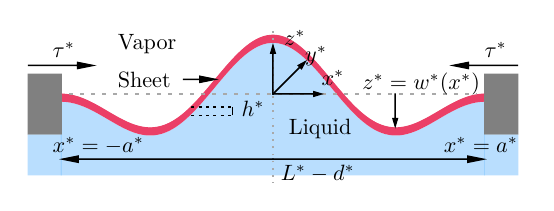
\begin{tikzpicture}

\definecolor{darkgray}{RGB}{169,169,169}
\definecolor{darkgray176}{RGB}{176,176,176}
\definecolor{gray}{RGB}{128,128,128}
\definecolor{indianred23563103}{RGB}{235,63,103}
\definecolor{lightskyblue138200253}{RGB}{138,200,253}

\begin{axis}[
axis equal image,
hide x axis,
hide y axis,
tick align=outside,
tick pos=left,
x grid style={darkgray176},
xlabel={0},
xmin=-0.03311, xmax=0.03311,
xtick style={color=black},
y grid style={darkgray176},
ymin=-0.010863663529839, ymax=0.00813693412661942,
ytick style={color=black}
]
\path [fill=lightskyblue138200253, fill opacity=0.6]
(axis cs:-0.0260467875630729,-0.00095)
--(axis cs:-0.0260467875630729,-0.00095)
--(axis cs:-0.0259887601975588,-0.000950265193764294)
--(axis cs:-0.0259307328320446,-0.000951060839657842)
--(axis cs:-0.0258727054665305,-0.000952386935837379)
--(axis cs:-0.0258146781010164,-0.000954243348798273)
--(axis cs:-0.0257566507355023,-0.000956629813394401)
--(axis cs:-0.0256986233699882,-0.000959545932885385)
--(axis cs:-0.0256405960044741,-0.0009629911790112)
--(axis cs:-0.02558256863896,-0.0009669648920941)
--(axis cs:-0.0255245412734459,-0.0009714662811679)
--(axis cs:-0.0254665139079318,-0.0009764944241347)
--(axis cs:-0.0254084865424177,-0.0009820482679484)
--(axis cs:-0.0253504591769036,-0.0009881266288259)
--(axis cs:-0.0252924318113895,-0.0009947281924857)
--(axis cs:-0.0252344044458754,-0.0010018515144127)
--(axis cs:-0.0251763770803613,-0.0010094950201512)
--(axis cs:-0.0251183497148472,-0.0010176570056243)
--(axis cs:-0.0250603223493331,-0.00102633563748)
--(axis cs:-0.025002294983819,-0.0010355289534653)
--(axis cs:-0.0249442676183049,-0.001045234862826)
--(axis cs:-0.0248862402527908,-0.0010554511467335)
--(axis cs:-0.0248282128872767,-0.0010661754587388)
--(axis cs:-0.0247701855217626,-0.0010774053252526)
--(axis cs:-0.0247121581562485,-0.0010891381460517)
--(axis cs:-0.0246541307907344,-0.0011013711948125)
--(axis cs:-0.0245961034252203,-0.00111410161967)
--(axis cs:-0.0245380760597062,-0.0011273264438032)
--(axis cs:-0.0244800486941921,-0.0011410425660469)
--(axis cs:-0.024422021328678,-0.001155246761529)
--(axis cs:-0.0243639939631638,-0.0011699356823334)
--(axis cs:-0.0243059665976497,-0.0011851058581895)
--(axis cs:-0.0242479392321356,-0.0012007536971861)
--(axis cs:-0.0241899118666215,-0.0012168754865111)
--(axis cs:-0.0241318845011074,-0.0012334673932171)
--(axis cs:-0.0240738571355933,-0.0012505254650108)
--(axis cs:-0.0240158297700792,-0.0012680456310682)
--(axis cs:-0.0239578024045651,-0.0012860237028747)
--(axis cs:-0.023899775039051,-0.0013044553750889)
--(axis cs:-0.0238417476735369,-0.0013233362264317)
--(axis cs:-0.0237837203080228,-0.0013426617205992)
--(axis cs:-0.0237256929425087,-0.0013624272071996)
--(axis cs:-0.0236676655769946,-0.0013826279227144)
--(axis cs:-0.0236096382114805,-0.0014032589914829)
--(axis cs:-0.0235516108459664,-0.00142431542671)
--(axis cs:-0.0234935834804523,-0.0014457921314979)
--(axis cs:-0.0234355561149382,-0.0014676838999004)
--(axis cs:-0.0233775287494241,-0.0014899854180001)
--(axis cs:-0.02331950138391,-0.0015126912650084)
--(axis cs:-0.0232614740183959,-0.001535795914388)
--(axis cs:-0.0232034466528818,-0.0015592937349971)
--(axis cs:-0.0231454192873677,-0.0015831789922564)
--(axis cs:-0.0230873919218536,-0.0016074458493369)
--(axis cs:-0.0230293645563395,-0.0016320883683701)
--(axis cs:-0.0229713371908254,-0.0016571005116786)
--(axis cs:-0.0229133098253113,-0.0016824761430286)
--(axis cs:-0.0228552824597972,-0.0017082090289024)
--(axis cs:-0.022797255094283,-0.0017342928397919)
--(axis cs:-0.0227392277287689,-0.0017607211515122)
--(axis cs:-0.0226812003632548,-0.0017874874465348)
--(axis cs:-0.0226231729977407,-0.0018145851153413)
--(axis cs:-0.0225651456322266,-0.0018420074577962)
--(axis cs:-0.0225071182667125,-0.0018697476845382)
--(axis cs:-0.0224490909011984,-0.0018977989183919)
--(axis cs:-0.0223910635356843,-0.0019261541957963)
--(axis cs:-0.0223330361701702,-0.0019548064682534)
--(axis cs:-0.0222750088046561,-0.0019837486037933)
--(axis cs:-0.022216981439142,-0.0020129733884583)
--(axis cs:-0.0221589540736279,-0.0020424735278035)
--(axis cs:-0.0221009267081138,-0.0020722416484151)
--(axis cs:-0.0220428993425997,-0.0021022702994453)
--(axis cs:-0.0219848719770856,-0.0021325519541642)
--(axis cs:-0.0219268446115715,-0.0021630790115269)
--(axis cs:-0.0218688172460574,-0.0021938437977579)
--(axis cs:-0.0218107898805433,-0.0022248385679495)
--(axis cs:-0.0217527625150292,-0.0022560555076774)
--(axis cs:-0.0216947351495151,-0.0022874867346291)
--(axis cs:-0.021636707784001,-0.002319124300249)
--(axis cs:-0.0215786804184869,-0.0023509601913962)
--(axis cs:-0.0215206530529728,-0.0023829863320169)
--(axis cs:-0.0214626256874587,-0.0024151945848308)
--(axis cs:-0.0214045983219446,-0.0024475767530302)
--(axis cs:-0.0213465709564305,-0.002480124581992)
--(axis cs:-0.0212885435909164,-0.0025128297610032)
--(axis cs:-0.0212305162254023,-0.0025456839249973)
--(axis cs:-0.0211724888598882,-0.002578678656304)
--(axis cs:-0.021114461494374,-0.0026118054864094)
--(axis cs:-0.0210564341288599,-0.0026450558977279)
--(axis cs:-0.0209984067633458,-0.0026784213253852)
--(axis cs:-0.0209403793978317,-0.002711893159011)
--(axis cs:-0.0208823520323176,-0.0027454627445428)
--(axis cs:-0.0208243246668035,-0.0027791213860387)
--(axis cs:-0.0207662973012894,-0.0028128603475)
--(axis cs:-0.0207082699357753,-0.0028466708547028)
--(axis cs:-0.0206502425702612,-0.0028805440970383)
--(axis cs:-0.0205922152047471,-0.0029144712293615)
--(axis cs:-0.020534187839233,-0.0029484433738474)
--(axis cs:-0.0204761604737189,-0.0029824516218552)
--(axis cs:-0.0204181331082048,-0.0030164870357999)
--(axis cs:-0.0203601057426907,-0.0030505406510301)
--(axis cs:-0.0203020783771766,-0.0030846034777124)
--(axis cs:-0.0202440510116625,-0.0031186665027225)
--(axis cs:-0.0201860236461484,-0.0031527206915414)
--(axis cs:-0.0201279962806343,-0.0031867569901566)
--(axis cs:-0.0200699689151202,-0.0032207663269691)
--(axis cs:-0.0200119415496061,-0.0032547396147045)
--(axis cs:-0.019953914184092,-0.0032886677523278)
--(axis cs:-0.0198958868185779,-0.0033225416269632)
--(axis cs:-0.0198378594530638,-0.0033563521158155)
--(axis cs:-0.0197798320875497,-0.0033900900880965)
--(axis cs:-0.0197218047220356,-0.0034237464069524)
--(axis cs:-0.0196637773565215,-0.0034573119313946)
--(axis cs:-0.0196057499910074,-0.0034907775182313)
--(axis cs:-0.0195477226254933,-0.0035241340240011)
--(axis cs:-0.0194896952599792,-0.0035573723069084)
--(axis cs:-0.019431667894465,-0.0035904832287575)
--(axis cs:-0.0193736405289509,-0.0036234576568893)
--(axis cs:-0.0193156131634368,-0.0036562864661163)
--(axis cs:-0.0192575857979227,-0.0036889605406574)
--(axis cs:-0.0191995584324086,-0.0037214707760725)
--(axis cs:-0.0191415310668945,-0.0037538080811952)
--(axis cs:-0.0190835037013804,-0.003785963380064)
--(axis cs:-0.0190254763358663,-0.0038179276138512)
--(axis cs:-0.0189674489703522,-0.0038496917427901)
--(axis cs:-0.0189094216048381,-0.0038812467480988)
--(axis cs:-0.018851394239324,-0.0039125836339006)
--(axis cs:-0.0187933668738099,-0.0039436934291412)
--(axis cs:-0.0187353395082958,-0.0039745671895024)
--(axis cs:-0.0186773121427817,-0.0040051959993101)
--(axis cs:-0.0186192847772676,-0.0040355709734386)
--(axis cs:-0.0185612574117535,-0.0040656832592097)
--(axis cs:-0.0185032300462394,-0.0040955240382859)
--(axis cs:-0.0184452026807253,-0.0041250845285578)
--(axis cs:-0.0183871753152112,-0.0041543559860256)
--(axis cs:-0.0183291479496971,-0.004183329706673)
--(axis cs:-0.018271120584183,-0.0042119970283357)
--(axis cs:-0.0182130932186689,-0.0042403493325605)
--(axis cs:-0.0181550658531548,-0.0042683780464584)
--(axis cs:-0.0180970384876407,-0.0042960746445482)
--(axis cs:-0.0180390111221266,-0.0043234306505924)
--(axis cs:-0.0179809837566125,-0.0043504376394242)
--(axis cs:-0.0179229563910984,-0.0043770872387641)
--(axis cs:-0.0178649290255843,-0.0044033711310288)
--(axis cs:-0.0178069016600702,-0.0044292810551283)
--(axis cs:-0.0177488742945561,-0.0044548088082534)
--(axis cs:-0.0176908469290419,-0.0044799462476529)
--(axis cs:-0.0176328195635278,-0.0045046852923988)
--(axis cs:-0.0175747921980137,-0.0045290179251406)
--(axis cs:-0.0175167648324996,-0.0045529361938479)
--(axis cs:-0.0174587374669855,-0.0045764322135405)
--(axis cs:-0.0174007101014714,-0.0045994981680062)
--(axis cs:-0.0173426827359573,-0.0046221263115058)
--(axis cs:-0.0172846553704432,-0.0046443089704646)
--(axis cs:-0.0172266280049291,-0.004666038545151)
--(axis cs:-0.017168600639415,-0.0046873075113404)
--(axis cs:-0.0171105732739009,-0.0047081084219658)
--(axis cs:-0.0170525459083868,-0.0047284339087529)
--(axis cs:-0.0169945185428727,-0.004748276683841)
--(axis cs:-0.0169364911773586,-0.0047676295413887)
--(axis cs:-0.0168784638118445,-0.0047864853591634)
--(axis cs:-0.0168204364463304,-0.004804837100116)
--(axis cs:-0.0167624090808163,-0.0048226778139384)
--(axis cs:-0.0167043817153022,-0.0048400006386051)
--(axis cs:-0.0166463543497881,-0.004856798801898)
--(axis cs:-0.016588326984274,-0.0048730656229136)
--(axis cs:-0.0165302996187599,-0.0048887945135536)
--(axis cs:-0.0164722722532458,-0.0049039789799969)
--(axis cs:-0.0164142448877317,-0.0049186126241543)
--(axis cs:-0.0163562175222176,-0.0049326891451044)
--(axis cs:-0.0162981901567035,-0.004946202340511)
--(axis cs:-0.0162401627911894,-0.0049591461080219)
--(axis cs:-0.0161821354256753,-0.0049715144466483)
--(axis cs:-0.0161241080601612,-0.0049833014581245)
--(axis cs:-0.016066080694647,-0.0049945013482481)
--(axis cs:-0.0160080533291329,-0.0050051084282006)
--(axis cs:-0.0159500259636188,-0.0050151171158466)
--(axis cs:-0.0158919985981047,-0.0050245219370138)
--(axis cs:-0.0158339712325906,-0.0050333175267513)
--(axis cs:-0.0157759438670765,-0.0050414986305666)
--(axis cs:-0.0157179165015624,-0.0050490601056428)
--(axis cs:-0.0156598891360483,-0.0050559969220319)
--(axis cs:-0.0156018617705342,-0.0050623041638287)
--(axis cs:-0.0155438344050201,-0.0050679770303207)
--(axis cs:-0.015485807039506,-0.0050730108371168)
--(axis cs:-0.0154277796739919,-0.0050774010172532)
--(axis cs:-0.0153697523084778,-0.0050811431222766)
--(axis cs:-0.0153117249429637,-0.005084232823304)
--(axis cs:-0.0152536975774496,-0.0050866659120601)
--(axis cs:-0.0151956702119355,-0.0050884383018905)
--(axis cs:-0.0151376428464214,-0.0050895460287518)
--(axis cs:-0.0150796154809073,-0.0050899852521776)
--(axis cs:-0.0150215881153932,-0.0050897522562207)
--(axis cs:-0.0149635607498791,-0.0050888434503707)
--(axis cs:-0.014905533384365,-0.005087255370448)
--(axis cs:-0.0148475060188509,-0.0050849846794718)
--(axis cs:-0.0147894786533368,-0.0050820281685051)
--(axis cs:-0.0147314512878227,-0.005078382757473)
--(axis cs:-0.0146734239223086,-0.0050740454959573)
--(axis cs:-0.0146153965567945,-0.005069013563965)
--(axis cs:-0.0145573691912804,-0.0050632842726713)
--(axis cs:-0.0144993418257662,-0.0050568550651379)
--(axis cs:-0.0144413144602522,-0.0050497235170041)
--(axis cs:-0.014383287094738,-0.0050418873371532)
--(axis cs:-0.0143252597292239,-0.0050333443683527)
--(axis cs:-0.0142672323637098,-0.0050240925878675)
--(axis cs:-0.0142092049981957,-0.0050141301080476)
--(axis cs:-0.0141511776326816,-0.0050034551768892)
--(axis cs:-0.0140931502671675,-0.0049920661785691)
--(axis cs:-0.0140351229016534,-0.0049799616339523)
--(axis cs:-0.0139770955361393,-0.0049671402010732)
--(axis cs:-0.0139190681706252,-0.0049536006755896)
--(axis cs:-0.0138610408051111,-0.0049393419912099)
--(axis cs:-0.013803013439597,-0.0049243632200929)
--(axis cs:-0.0137449860740829,-0.004908663573221)
--(axis cs:-0.0136869587085688,-0.0048922424007455)
--(axis cs:-0.0136289313430547,-0.0048750991923051)
--(axis cs:-0.0135709039775406,-0.0048572335773168)
--(axis cs:-0.0135128766120265,-0.0048386453252388)
--(axis cs:-0.0134548492465124,-0.0048193343458073)
--(axis cs:-0.0133968218809983,-0.0047993006892437)
--(axis cs:-0.0133387945154842,-0.0047785445464361)
--(axis cs:-0.0132807671499701,-0.004757066249092)
--(axis cs:-0.013222739784456,-0.0047348662698632)
--(axis cs:-0.0131647124189419,-0.0047119452224437)
--(axis cs:-0.0131066850534278,-0.0046883038616392)
--(axis cs:-0.0130486576879137,-0.0046639430834091)
--(axis cs:-0.0129906303223996,-0.0046388639248803)
--(axis cs:-0.0129326029568855,-0.0046130675643335)
--(axis cs:-0.0128745755913714,-0.0045865553211618)
--(axis cs:-0.0128165482258572,-0.0045593286558008)
--(axis cs:-0.0127585208603431,-0.0045313891696316)
--(axis cs:-0.012700493494829,-0.0045027386048555)
--(axis cs:-0.0126424661293149,-0.0044733788443407)
--(axis cs:-0.0125844387638008,-0.0044433119114421)
--(axis cs:-0.0125264113982867,-0.0044125399697922)
--(axis cs:-0.0124683840327726,-0.004381065323065)
--(axis cs:-0.0124103566672585,-0.0043488904147121)
--(axis cs:-0.0123523293017444,-0.0043160178276705)
--(axis cs:-0.0122943019362303,-0.0042824502840439)
--(axis cs:-0.0122362745707162,-0.0042481906447556)
--(axis cs:-0.0121782472052021,-0.0042132419091739)
--(axis cs:-0.012120219839688,-0.0041776072147107)
--(axis cs:-0.0120621924741739,-0.0041412898363918)
--(axis cs:-0.0120041651086598,-0.0041042931864011)
--(axis cs:-0.0119461377431457,-0.0040666208135963)
--(axis cs:-0.0118881103776316,-0.0040282764029982)
--(axis cs:-0.0118300830121175,-0.0039892637752531)
--(axis cs:-0.0117720556466034,-0.0039495868860678)
--(axis cs:-0.0117140282810893,-0.0039092498256181)
--(axis cs:-0.0116560009155752,-0.0038682568179303)
--(axis cs:-0.0115979735500611,-0.0038266122202361)
--(axis cs:-0.011539946184547,-0.0037843205223014)
--(axis cs:-0.0114819188190329,-0.0037413863457285)
--(axis cs:-0.0114238914535188,-0.0036978144432314)
--(axis cs:-0.0113658640880047,-0.0036536096978864)
--(axis cs:-0.0113078367224906,-0.003608777122355)
--(axis cs:-0.0112498093569765,-0.0035633218580827)
--(axis cs:-0.0111917819914624,-0.0035172491744708)
--(axis cs:-0.0111337546259482,-0.0034705644680232)
--(axis cs:-0.0110757272604341,-0.0034232732614678)
--(axis cs:-0.01101769989492,-0.0033753812028528)
--(axis cs:-0.0109596725294059,-0.0033268940646176)
--(axis cs:-0.0109016451638918,-0.0032778177426395)
--(axis cs:-0.0108436177983777,-0.0032281582552545)
--(axis cs:-0.0107855904328636,-0.0031779217422552)
--(axis cs:-0.0107275630673495,-0.0031271144638632)
--(axis cs:-0.0106695357018354,-0.0030757427996777)
--(axis cs:-0.0106115083363213,-0.0030238132476002)
--(axis cs:-0.0105534809708072,-0.002971332422736)
--(axis cs:-0.0104954536052931,-0.0029183070562708)
--(axis cs:-0.010437426239779,-0.0028647439943259)
--(axis cs:-0.0103793988742649,-0.0028106501967886)
--(axis cs:-0.0103213715087508,-0.0027560327361208)
--(axis cs:-0.0102633441432367,-0.0027008987961445)
--(axis cs:-0.0102053167777226,-0.0026452556708052)
--(axis cs:-0.0101472894122085,-0.0025891107629128)
--(axis cs:-0.0100892620466944,-0.0025324715828607)
--(axis cs:-0.0100312346811803,-0.0024753457473236)
--(axis cs:-0.0099732073156662,-0.002417740977933)
--(axis cs:-0.0099151799501521,-0.0023596650999325)
--(axis cs:-0.009857152584638,-0.0023011260408115)
--(axis cs:-0.0097991252191239,-0.0022421318289185)
--(axis cs:-0.0097410978536098,-0.0021826905920538)
--(axis cs:-0.0096830704880957,-0.0021228105560424)
--(axis cs:-0.0096250431225816,-0.002062500043287)
--(axis cs:-0.0095670157570675,-0.0020017674713008)
--(axis cs:-0.0095089883915534,-0.001940621351222)
--(axis cs:-0.0094509610260392,-0.0018790702863083)
--(axis cs:-0.0093929336605251,-0.0018171229704134)
--(axis cs:-0.009334906295011,-0.001754788186445)
--(axis cs:-0.0092768789294969,-0.0016920748048038)
--(axis cs:-0.0092188515639828,-0.0016289917818061)
--(axis cs:-0.0091608241984687,-0.0015655481580875)
--(axis cs:-0.0091027968329546,-0.0015017530569903)
--(axis cs:-0.0090447694674405,-0.0014376156829333)
--(axis cs:-0.0089867421019264,-0.0013731453197656)
--(axis cs:-0.0089287147364123,-0.0013083513291039)
--(axis cs:-0.0088706873708982,-0.0012432431486535)
--(axis cs:-0.0088126600053841,-0.0011778302905138)
--(axis cs:-0.00875463263987,-0.0011121223394691)
--(axis cs:-0.0086966052743559,-0.0010461289512635)
--(axis cs:-0.0086385779088418,-0.0009798598508618)
--(axis cs:-0.0085805505433277,-0.0009133248306954)
--(axis cs:-0.0085225231778136,-0.0008465337488949)
--(axis cs:-0.0084644958122995,-0.000779496527509)
--(axis cs:-0.0084064684467854,-0.0007122231507094)
--(axis cs:-0.0083484410812713,-0.0006447236629836)
--(axis cs:-0.0082904137157572,-0.0005770081673146)
--(axis cs:-0.0082323863502431,-0.0005090868233482)
--(axis cs:-0.008174358984729,-0.000440969845549)
--(axis cs:-0.0081163316192149,-0.0003726675013445)
--(axis cs:-0.0080583042537008,-0.0003041901092578)
--(axis cs:-0.0080002768881867,-0.0002355480370296)
--(axis cs:-0.0079422495226726,-0.0001667516997302)
--(axis cs:-0.0078842221571585,-9.78115578609e-05)
--(axis cs:-0.0078261947916443,-2.87381154455e-05)
--(axis cs:-0.0077681674261302,4.04580818869001e-05)
--(axis cs:-0.0077101400606161,0.0001097664488288)
--(axis cs:-0.007652112695102,0.000179176362329)
--(axis cs:-0.0075940853295879,0.0002486771635367)
--(axis cs:-0.0075360579640738,0.0003182581597521)
--(axis cs:-0.0074780305985597,0.0003879086263859)
--(axis cs:-0.0074200032330456,0.0004576178089245)
--(axis cs:-0.0073619758675315,0.0005273749249031)
--(axis cs:-0.0073039485020174,0.0005971691658846)
--(axis cs:-0.0072459211365033,0.0006669896994445)
--(axis cs:-0.0071878937709892,0.0007368256711616)
--(axis cs:-0.0071298664054751,0.0008066662066133)
--(axis cs:-0.007071839039961,0.0008765004133766)
--(axis cs:-0.0070138116744469,0.000946317383033)
--(axis cs:-0.0069557843089328,0.0010161061931771)
--(axis cs:-0.0068977569434187,0.0010858559094298)
--(axis cs:-0.0068397295779046,0.0011555555874539)
--(axis cs:-0.0067817022123905,0.0012251942749728)
--(axis cs:-0.0067236748468764,0.0012947610137919)
--(axis cs:-0.0066656474813623,0.0013642448418217)
--(axis cs:-0.0066076201158482,0.001433634795103)
--(axis cs:-0.0065495927503341,0.0015029199098332)
--(axis cs:-0.00649156538482,0.0015720892243932)
--(axis cs:-0.0064335380193059,0.0016411317813754)
--(axis cs:-0.0063755106537918,0.0017100366296114)
--(axis cs:-0.0063174832882777,0.0017787928261994)
--(axis cs:-0.0062594559227636,0.0018473894385313)
--(axis cs:-0.0062014285572495,0.0019158155463182)
--(axis cs:-0.0061434011917353,0.0019840602436151)
--(axis cs:-0.0060853738262212,0.0020521126408427)
--(axis cs:-0.0060273464607071,0.0021199618668086)
--(axis cs:-0.005969319095193,0.0021875970707238)
--(axis cs:-0.0059112917296789,0.002255007424218)
--(axis cs:-0.0058532643641648,0.0023221821233506)
--(axis cs:-0.0057952369986507,0.0023891103906177)
--(axis cs:-0.0057372096331366,0.0024557814769555)
--(axis cs:-0.0056791822676225,0.0025221846637386)
--(axis cs:-0.0056211549021084,0.0025883092647736)
--(axis cs:-0.0055631275365943,0.0026541446282875)
--(axis cs:-0.0055051001710802,0.0027196801389097)
--(axis cs:-0.0054470728055661,0.0027849052196483)
--(axis cs:-0.005389045440052,0.0028498093338603)
--(axis cs:-0.0053310180745379,0.0029143819872138)
--(axis cs:-0.0052729907090238,0.0029786127296439)
--(axis cs:-0.0052149633435097,0.0030424911573005)
--(axis cs:-0.0051569359779956,0.0031060069144879)
--(axis cs:-0.0050989086124815,0.0031691496955965)
--(axis cs:-0.0050408812469674,0.0032319092470251)
--(axis cs:-0.0049828538814533,0.0032942753690946)
--(axis cs:-0.0049248265159392,0.0033562379179513)
--(axis cs:-0.0048667991504251,0.0034177868074615)
--(axis cs:-0.004808771784911,0.0034789120110947)
--(axis cs:-0.0047507444193969,0.0035396035637965)
--(axis cs:-0.0046927170538828,0.003599851563851)
--(axis cs:-0.0046346896883687,0.0036596461747309)
--(axis cs:-0.0045766623228546,0.0037189776269367)
--(axis cs:-0.0045186349573404,0.0037778362198231)
--(axis cs:-0.0044606075918263,0.0038362123234136)
--(axis cs:-0.0044025802263122,0.0038940963802016)
--(axis cs:-0.0043445528607981,0.003951478906939)
--(axis cs:-0.004286525495284,0.0040083504964109)
--(axis cs:-0.0042284981297699,0.0040647018191964)
--(axis cs:-0.0041704707642558,0.0041205236254156)
--(axis cs:-0.0041124433987417,0.0041758067464615)
--(axis cs:-0.0040544160332276,0.0042305420967175)
--(axis cs:-0.0039963886677135,0.0042847206752595)
--(axis cs:-0.0039383613021994,0.0043383335675425)
--(axis cs:-0.0038803339366853,0.0043913719470711)
--(axis cs:-0.0038223065711712,0.0044438270770541)
--(axis cs:-0.0037642792056571,0.0044956903120428)
--(axis cs:-0.003706251840143,0.0045469530995516)
--(axis cs:-0.0036482244746289,0.0045976069816624)
--(axis cs:-0.0035901971091148,0.0046476435966109)
--(axis cs:-0.0035321697436007,0.0046970546803555)
--(axis cs:-0.0034741423780866,0.0047458320681279)
--(axis cs:-0.0034161150125725,0.0047939676959654)
--(axis cs:-0.0033580876470584,0.0048414536022244)
--(axis cs:-0.0033000602815443,0.0048882819290753)
--(axis cs:-0.0032420329160302,0.0049344449239776)
--(axis cs:-0.0031840055505161,0.0049799349411358)
--(axis cs:-0.003125978185002,0.0050247444429354)
--(axis cs:-0.0030679508194879,0.0050688660013585)
--(axis cs:-0.0030099234539738,0.0051122922993799)
--(axis cs:-0.0029518960884597,0.0051550161323409)
--(axis cs:-0.0028938687229456,0.0051970304093041)
--(axis cs:-0.0028358413574314,0.0052383281543854)
--(axis cs:-0.0027778139919173,0.0052789025080655)
--(axis cs:-0.0027197866264032,0.0053187467284794)
--(axis cs:-0.0026617592608891,0.0053578541926837)
--(axis cs:-0.002603731895375,0.0053962183979018)
--(axis cs:-0.0025457045298609,0.0054338329627473)
--(axis cs:-0.0024876771643468,0.0054706916284235)
--(axis cs:-0.0024296497988327,0.0055067882599011)
--(axis cs:-0.0023716224333186,0.0055421168470718)
--(axis cs:-0.0023135950678045,0.0055766715058794)
--(axis cs:-0.0022555677022904,0.0056104464794266)
--(axis cs:-0.0021975403367763,0.0056434361390583)
--(axis cs:-0.0021395129712622,0.0056756349854209)
--(axis cs:-0.0020814856057481,0.0057070376494972)
--(axis cs:-0.002023458240234,0.0057376388936169)
--(axis cs:-0.0019654308747199,0.0057674336124427)
--(axis cs:-0.0019074035092058,0.005796416833931)
--(axis cs:-0.0018493761436917,0.0058245837202684)
--(axis cs:-0.0017913487781776,0.0058519295687821)
--(axis cs:-0.0017333214126635,0.0058784498128259)
--(axis cs:-0.0016752940471494,0.0059041400226397)
--(axis cs:-0.0016172666816353,0.0059289959061837)
--(axis cs:-0.0015592393161212,0.0059530133099471)
--(axis cs:-0.0015012119506071,0.0059761882197301)
--(axis cs:-0.001443184585093,0.0059985167614001)
--(axis cs:-0.0013851572195789,0.0060199952016214)
--(axis cs:-0.0013271298540648,0.0060406199485585)
--(axis cs:-0.0012691024885507,0.006060387552553)
--(axis cs:-0.0012110751230365,0.0060792947067731)
--(axis cs:-0.0011530477575224,0.0060973382478368)
--(axis cs:-0.0010950203920083,0.0061145151564082)
--(axis cs:-0.0010369930264942,0.0061308225577661)
--(axis cs:-0.0009789656609801,0.0061462577223458)
--(axis cs:-0.000920938295466,0.0061608180662536)
--(axis cs:-0.0008629109299519,0.0061745011517535)
--(axis cs:-0.0008048835644378,0.0061873046877267)
--(axis cs:-0.0007468561989237,0.0061992265301038)
--(axis cs:-0.0006888288334096,0.0062102646822681)
--(axis cs:-0.0006308014678955,0.0062204172954327)
--(axis cs:-0.0005727741023814,0.0062296826689883)
--(axis cs:-0.0005147467368673,0.0062380592508244)
--(axis cs:-0.0004567193713532,0.0062455456376213)
--(axis cs:-0.0003986920058391,0.0062521405751149)
--(axis cs:-0.000340664640325,0.0062578429583332)
--(axis cs:-0.0002826372748109,0.0062626518318042)
--(axis cs:-0.0002246099092968,0.0062665663897367)
--(axis cs:-0.0001665825437827,0.0062695859761714)
--(axis cs:-0.0001085551782686,0.0062717100851051)
--(axis cs:-5.05278127545e-05,0.0062729383605859)
--(axis cs:7.49955275957484e-06,0.0062732705967804)
--(axis cs:6.55269182736e-05,0.0062727067380123)
--(axis cs:0.0001235542837877,0.0062712468787732)
--(axis cs:0.0001815816493018,0.0062688912637045)
--(axis cs:0.0002396090148159,0.0062656402875514)
--(axis cs:0.00029763638033,0.0062614944950884)
--(axis cs:0.0003556637458441,0.006256454581017)
--(axis cs:0.0004136911113583,0.006250521389834)
--(axis cs:0.0004717184768724,0.0062436959156731)
--(axis cs:0.0005297458423865,0.0062359793021168)
--(axis cs:0.0005877732079006,0.0062273728419815)
--(axis cs:0.0006458005734147,0.0062178779770732)
--(axis cs:0.0007038279389288,0.0062074962979162)
--(axis cs:0.0007618553044429,0.0061962295434529)
--(axis cs:0.000819882669957,0.0061840796007164)
--(axis cs:0.0008779100354711,0.0061710485044744)
--(axis cs:0.0009359374009852,0.0061571384368463)
--(axis cs:0.0009939647664993,0.0061423517268912)
--(axis cs:0.0010519921320134,0.0061266908501698)
--(axis cs:0.0011100194975275,0.0061101584282769)
--(axis cs:0.0011680468630416,0.0060927572283482)
--(axis cs:0.0012260742285557,0.0060744901625383)
--(axis cs:0.0012841015940698,0.0060553602874725)
--(axis cs:0.0013421289595839,0.0060353708036701)
--(axis cs:0.001400156325098,0.0060145250549421)
--(axis cs:0.0014581836906121,0.0059928265277606)
--(axis cs:0.0015162110561262,0.0059702788506027)
--(axis cs:0.0015742384216403,0.0059468857932659)
--(axis cs:0.0016322657871544,0.005922651266159)
--(axis cs:0.0016902931526685,0.0058975793195649)
--(axis cs:0.0017483205181826,0.0058716741428779)
--(axis cs:0.0018063478836967,0.0058449400638145)
--(axis cs:0.0018643752492108,0.0058173815475987)
--(axis cs:0.0019224026147249,0.0057890031961207)
--(axis cs:0.001980429980239,0.0057598097470708)
--(axis cs:0.0020384573457531,0.005729806073047)
--(axis cs:0.0020964847112673,0.0056989971806378)
--(axis cs:0.0021545120767814,0.0056673882094794)
--(axis cs:0.0022125394422955,0.0056349844312886)
--(axis cs:0.0022705668078096,0.0056017912488703)
--(axis cs:0.0023285941733237,0.0055678141951005)
--(axis cs:0.0023866215388378,0.0055330589318852)
--(axis cs:0.0024446489043519,0.0054975312490949)
--(axis cs:0.002502676269866,0.0054612370634753)
--(axis cs:0.0025607036353801,0.005424182417534)
--(axis cs:0.0026187310008942,0.0053863734784036)
--(axis cs:0.0026767583664083,0.0053478165366819)
--(axis cs:0.0027347857319224,0.0053085180052486)
--(axis cs:0.0027928130974365,0.0052684844180596)
--(axis cs:0.0028508404629506,0.0052277224289176)
--(axis cs:0.0029088678284647,0.0051862388102218)
--(axis cs:0.0029668951939788,0.0051440404516942)
--(axis cs:0.0030249225594929,0.0051011343590849)
--(axis cs:0.003082949925007,0.0050575276528549)
--(axis cs:0.0031409772905211,0.0050132275668382)
--(axis cs:0.0031990046560352,0.0049682414468826)
--(axis cs:0.0032570320215493,0.0049225767494693)
--(axis cs:0.0033150593870634,0.0048762410403122)
--(axis cs:0.0033730867525775,0.0048292419929372)
--(axis cs:0.0034311141180916,0.0047815873872405)
--(axis cs:0.0034891414836057,0.004733285108028)
--(axis cs:0.0035471688491198,0.0046843431435352)
--(axis cs:0.0036051962146339,0.0046347695839272)
--(axis cs:0.003663223580148,0.0045845726197802)
--(axis cs:0.0037212509456621,0.004533760540545)
--(axis cs:0.0037792783111762,0.004482341732991)
--(axis cs:0.0038373056766904,0.0044303246796332)
--(axis cs:0.0038953330422045,0.0043777179571411)
--(axis cs:0.0039533604077186,0.0043245302347299)
--(axis cs:0.0040113877732327,0.0042707702725355)
--(axis cs:0.0040694151387468,0.0042164469199718)
--(axis cs:0.0041274425042609,0.0041615691140721)
--(axis cs:0.004185469869775,0.0041061458778145)
--(axis cs:0.0042434972352891,0.0040501863184309)
--(axis cs:0.0043015246008032,0.0039936996257012)
--(axis cs:0.0043595519663173,0.0039366950702318)
--(axis cs:0.0044175793318314,0.0038791820017202)
--(axis cs:0.0044756066973455,0.0038211698472038)
--(axis cs:0.0045336340628596,0.003762668109296)
--(axis cs:0.0045916614283737,0.0037036863644075)
--(axis cs:0.0046496887938878,0.0036442342609547)
--(axis cs:0.0047077161594019,0.0035843215175549)
--(axis cs:0.004765743524916,0.0035239579212088)
--(axis cs:0.0048237708904301,0.0034631533254706)
--(axis cs:0.0048817982559442,0.0034019176486059)
--(axis cs:0.0049398256214583,0.0033402608717384)
--(axis cs:0.0049978529869724,0.0032781930369852)
--(axis cs:0.0050558803524865,0.0032157242455805)
--(axis cs:0.0051139077180006,0.0031528646559898)
--(axis cs:0.0051719350835147,0.003089624482013)
--(axis cs:0.0052299624490288,0.0030260139908785)
--(axis cs:0.0052879898145429,0.0029620435013268)
--(axis cs:0.005346017180057,0.0028977233816861)
--(axis cs:0.0054040445455711,0.0028330640479385)
--(axis cs:0.0054620719110853,0.0027680759617783)
--(axis cs:0.0055200992765994,0.0027027696286617)
--(axis cs:0.0055781266421135,0.0026371555958498)
--(axis cs:0.0056361540076276,0.0025712444504435)
--(axis cs:0.0056941813731417,0.0025050468174126)
--(axis cs:0.0057522087386558,0.0024385733576175)
--(axis cs:0.0058102361041699,0.0023718347658253)
--(axis cs:0.005868263469684,0.0023048417687207)
--(axis cs:0.0059262908351981,0.0022376051229103)
--(axis cs:0.0059843182007122,0.0021701356129237)
--(axis cs:0.0060423455662263,0.0021024440492087)
--(axis cs:0.0061003729317404,0.0020345412661233)
--(axis cs:0.0061584002972545,0.0019664381199237)
--(axis cs:0.0062164276627686,0.0018981454867484)
--(axis cs:0.0062744550282827,0.0018296742606007)
--(axis cs:0.0063324823937968,0.0017610353513271)
--(axis cs:0.0063905097593109,0.001692239682595)
--(axis cs:0.006448537124825,0.0016232981898673)
--(axis cs:0.0065065644903391,0.001554221818377)
--(axis cs:0.0065645918558532,0.0014850215210994)
--(axis cs:0.0066226192213673,0.0014157082567252)
--(axis cs:0.0066806465868814,0.001346292987632)
--(axis cs:0.0067386739523955,0.0012767866778573)
--(axis cs:0.0067967013179096,0.0012072002910712)
--(axis cs:0.0068547286834237,0.0011375447885503)
--(axis cs:0.0069127560489378,0.0010678311271533)
--(axis cs:0.0069707834144519,0.0009980702572983)
--(axis cs:0.007028810779966,0.0009282731209418)
--(axis cs:0.0070868381454802,0.0008584506495611)
--(axis cs:0.0071448655109943,0.0007886137621388)
--(axis cs:0.0072028928765084,0.0007187733631513)
--(axis cs:0.0072609202420225,0.0006489403405607)
--(axis cs:0.0073189476075366,0.0005791255638111)
--(axis cs:0.0073769749730507,0.000509339881829)
--(axis cs:0.0074350023385648,0.0004395941210292)
--(axis cs:0.0074930297040789,0.0003698990833254)
--(axis cs:0.007551057069593,0.0003002655441467)
--(axis cs:0.0076090844351071,0.0002307042504607)
--(axis cs:0.0076671118006212,0.0001612259188018)
--(axis cs:0.0077251391661353,9.1841233308e-05)
--(axis cs:0.0077831665316494,2.2560843763e-05)
--(axis cs:0.0078411938971635,-4.6604636352e-05)
--(axis cs:0.0078992212626776,-0.0001156446318008)
--(axis cs:0.0079572486281917,-0.0001845486075241)
--(axis cs:0.0080152759937058,-0.0002533060705646)
--(axis cs:0.0080733033592199,-0.0003219065719818)
--(axis cs:0.008131330724734,-0.0003903397087577)
--(axis cs:0.0081893580902481,-0.0004585951256928)
--(axis cs:0.0082473854557622,-0.0005266625172919)
--(axis cs:0.0083054128212763,-0.0005945316296392)
--(axis cs:0.0083634401867904,-0.0006621922622624)
--(axis cs:0.0084214675523045,-0.0007296342699856)
--(axis cs:0.0084794949178186,-0.000796847564771)
--(axis cs:0.0085375222833327,-0.0008638221175477)
--(axis cs:0.0085955496488468,-0.0009305479600291)
--(axis cs:0.0086535770143609,-0.0009970151865167)
--(axis cs:0.0087116043798751,-0.001063213955692)
--(axis cs:0.0087696317453892,-0.0011291344923936)
--(axis cs:0.0088276591109033,-0.0011947670893817)
--(axis cs:0.0088856864764174,-0.001260102109088)
--(axis cs:0.0089437138419315,-0.0013251299853514)
--(axis cs:0.0090017412074456,-0.0013898412251388)
--(axis cs:0.0090597685729597,-0.0014542264102508)
--(axis cs:0.0091177959384738,-0.0015182761990121)
--(axis cs:0.0091758233039879,-0.0015819813279464)
--(axis cs:0.009233850669502,-0.0016453326134344)
--(axis cs:0.0092918780350161,-0.0017083209533569)
--(axis cs:0.0093499054005302,-0.0017709373287194)
--(axis cs:0.0094079327660443,-0.0018331728052611)
--(axis cs:0.0094659601315584,-0.0018950185350463)
--(axis cs:0.0095239874970725,-0.0019564657580374)
--(axis cs:0.0095820148625866,-0.0020175058036514)
--(axis cs:0.0096400422281007,-0.0020781300922963)
--(axis cs:0.0096980695936148,-0.0021383301368913)
--(axis cs:0.0097560969591289,-0.0021980975443657)
--(axis cs:0.009814124324643,-0.002257424017141)
--(axis cs:0.0098721516901571,-0.0023163013545921)
--(axis cs:0.0099301790556712,-0.0023747214544891)
--(axis cs:0.0099882064211853,-0.0024326763144199)
--(axis cs:0.0100462337866994,-0.002490158033192)
--(axis cs:0.0101042611522135,-0.0025471588122137)
--(axis cs:0.0101622885177276,-0.0026036709568549)
--(axis cs:0.0102203158832417,-0.0026596868777869)
--(axis cs:0.0102783432487558,-0.0027151990923009)
--(axis cs:0.01033637061427,-0.0027702002256047)
--(axis cs:0.0103943979797841,-0.0028246830120981)
--(axis cs:0.0104524253452982,-0.0028786402966263)
--(axis cs:0.0105104527108123,-0.0029320650357105)
--(axis cs:0.0105684800763264,-0.0029849502987567)
--(axis cs:0.0106265074418405,-0.0030372892692415)
--(axis cs:0.0106845348073546,-0.0030890752458751)
--(axis cs:0.0107425621728687,-0.0031403016437409)
--(axis cs:0.0108005895383828,-0.0031909619954122)
--(axis cs:0.0108586169038969,-0.0032410499520447)
--(axis cs:0.010916644269411,-0.003290559284446)
--(axis cs:0.0109746716349251,-0.0033394838841205)
--(axis cs:0.0110326990004392,-0.0033878177642905)
--(axis cs:0.0110907263659533,-0.0034355550608927)
--(axis cs:0.0111487537314674,-0.0034826900335504)
--(axis cs:0.0112067810969815,-0.0035292170665205)
--(axis cs:0.0112648084624956,-0.0035751306696162)
--(axis cs:0.0113228358280097,-0.0036204254791044)
--(axis cs:0.0113808631935238,-0.0036650962585775)
--(axis cs:0.0114388905590379,-0.0037091378998003)
--(axis cs:0.011496917924552,-0.0037525454235308)
--(axis cs:0.0115549452900661,-0.0037953139803162)
--(axis cs:0.0116129726555802,-0.0038374388512615)
--(axis cs:0.0116710000210943,-0.0038789154487739)
--(axis cs:0.0117290273866084,-0.0039197393172793)
--(axis cs:0.0117870547521225,-0.0039599061339142)
--(axis cs:0.0118450821176366,-0.0039994117091896)
--(axis cs:0.0119031094831507,-0.0040382519876296)
--(axis cs:0.0119611368486648,-0.0040764230483826)
--(axis cs:0.012019164214179,-0.0041139211058063)
--(axis cs:0.0120771915796931,-0.0041507425100251)
--(axis cs:0.0121352189452072,-0.0041868837474614)
--(axis cs:0.0121932463107213,-0.0042223414413392)
--(axis cs:0.0122512736762354,-0.004257112352161)
--(axis cs:0.0123093010417495,-0.0042911933781567)
--(axis cs:0.0123673284072636,-0.0043245815557064)
--(axis cs:0.0124253557727777,-0.0043572740597346)
--(axis cs:0.0124833831382918,-0.0043892682040776)
--(axis cs:0.0125414105038059,-0.0044205614418237)
--(axis cs:0.01259943786932,-0.0044511513656245)
--(axis cs:0.0126574652348341,-0.0044810357079803)
--(axis cs:0.0127154926003482,-0.0045102123414964)
--(axis cs:0.0127735199658623,-0.0045386792791127)
--(axis cs:0.0128315473313764,-0.0045664346743046)
--(axis cs:0.0128895746968905,-0.0045934768212569)
--(axis cs:0.0129476020624046,-0.0046198041550099)
--(axis cs:0.0130056294279187,-0.0046454152515768)
--(axis cs:0.0130636567934328,-0.0046703088280343)
--(axis cs:0.0131216841589469,-0.0046944837425845)
--(axis cs:0.013179711524461,-0.0047179389945898)
--(axis cs:0.0132377388899751,-0.0047406737245792)
--(axis cs:0.0132957662554892,-0.0047626872142272)
--(axis cs:0.0133537936210033,-0.0047839788863046)
--(axis cs:0.0134118209865174,-0.0048045483046017)
--(axis cs:0.0134698483520315,-0.0048243951738238)
--(axis cs:0.0135278757175456,-0.0048435193394584)
--(axis cs:0.0135859030830597,-0.0048619207876156)
--(axis cs:0.0136439304485738,-0.0048795996448399)
--(axis cs:0.013701957814088,-0.004896556177895)
--(axis cs:0.0137599851796021,-0.0049127907935207)
--(axis cs:0.0138180125451162,-0.0049283040381624)
--(axis cs:0.0138760399106303,-0.0049430965976733)
--(axis cs:0.0139340672761444,-0.0049571692969887)
--(axis cs:0.0139920946416585,-0.0049705230997738)
--(axis cs:0.0140501220071726,-0.0049831591080435)
--(axis cs:0.0141081493726867,-0.0049950785617552)
--(axis cs:0.0141661767382008,-0.0050062828383751)
--(axis cs:0.0142242041037149,-0.0050167734524172)
--(axis cs:0.014282231469229,-0.0050265520549547)
--(axis cs:0.0143402588347431,-0.005035620433106)
--(axis cs:0.0143982862002572,-0.0050439805094931)
--(axis cs:0.0144563135657713,-0.0050516343416738)
--(axis cs:0.0145143409312854,-0.0050585841215475)
--(axis cs:0.0145723682967995,-0.0050648321747344)
--(axis cs:0.0146303956623136,-0.0050703809599292)
--(axis cs:0.0146884230278277,-0.0050752330682281)
--(axis cs:0.0147464503933418,-0.0050793912224305)
--(axis cs:0.0148044777588559,-0.0050828582763143)
--(axis cs:0.01486250512437,-0.0050856372138866)
--(axis cs:0.0149205324898841,-0.0050877311486079)
--(axis cs:0.0149785598553982,-0.0050891433225921)
--(axis cs:0.0150365872209123,-0.0050898771057806)
--(axis cs:0.0150946145864264,-0.0050899359950916)
--(axis cs:0.0151526419519405,-0.0050893236135455)
--(axis cs:0.0152106693174546,-0.0050880437093646)
--(axis cs:0.0152686966829687,-0.005086100155049)
--(axis cs:0.0153267240484828,-0.0050834969464287)
--(axis cs:0.015384751413997,-0.0050802382016908)
--(axis cs:0.0154427787795111,-0.0050763281603838)
--(axis cs:0.0155008061450252,-0.0050717711823979)
--(axis cs:0.0155588335105393,-0.005066571746922)
--(axis cs:0.0156168608760534,-0.0050607344513776)
--(axis cs:0.0156748882415675,-0.0050542640103297)
--(axis cs:0.0157329156070816,-0.0050471652543753)
--(axis cs:0.0157909429725957,-0.005039443129009)
--(axis cs:0.0158489703381098,-0.0050311026934667)
--(axis cs:0.0159069977036239,-0.005022149119547)
--(axis cs:0.015965025069138,-0.0050125876904114)
--(axis cs:0.0160230524346521,-0.0050024237993623)
--(axis cs:0.0160810798001662,-0.0049916629485999)
--(axis cs:0.0161391071656803,-0.004980310747959)
--(axis cs:0.0161971345311944,-0.0049683729136234)
--(axis cs:0.0162551618967085,-0.0049558552668215)
--(axis cs:0.0163131892622226,-0.0049427637325003)
--(axis cs:0.0163712166277367,-0.0049291043379807)
--(axis cs:0.0164292439932508,-0.0049148832115919)
--(axis cs:0.0164872713587649,-0.0049001065812876)
--(axis cs:0.016545298724279,-0.004884780773242)
--(axis cs:0.0166033260897931,-0.0048689122104278)
--(axis cs:0.0166613534553072,-0.0048525074111753)
--(axis cs:0.0167193808208213,-0.0048355729877132)
--(axis cs:0.0167774081863354,-0.0048181156446917)
--(axis cs:0.0168354355518495,-0.004800142177688)
--(axis cs:0.0168934629173636,-0.0047816594716938)
--(axis cs:0.0169514902828777,-0.0047626744995868)
--(axis cs:0.0170095176483918,-0.0047431943205846)
--(axis cs:0.0170675450139059,-0.0047232260786827)
--(axis cs:0.0171255723794201,-0.0047027770010761)
--(axis cs:0.0171835997449342,-0.0046818543965657)
--(axis cs:0.0172416271104483,-0.004660465653948)
--(axis cs:0.0172996544759624,-0.0046386182403917)
--(axis cs:0.0173576818414765,-0.0046163196997972)
--(axis cs:0.0174157092069906,-0.0045935776511434)
--(axis cs:0.0174737365725047,-0.0045703997868196)
--(axis cs:0.0175317639380188,-0.0045467938709439)
--(axis cs:0.0175897913035329,-0.0045227677376678)
--(axis cs:0.017647818669047,-0.0044983292894679)
--(axis cs:0.0177058460345611,-0.0044734864954251)
--(axis cs:0.0177638734000752,-0.0044482473894911)
--(axis cs:0.0178219007655893,-0.0044226200687427)
--(axis cs:0.0178799281311034,-0.0043966126916248)
--(axis cs:0.0179379554966175,-0.004370233476182)
--(axis cs:0.0179959828621316,-0.0043434906982784)
--(axis cs:0.0180540102276457,-0.0043163926898083)
--(axis cs:0.0181120375931598,-0.0042889478368951)
--(axis cs:0.0181700649586739,-0.0042611645780812)
--(axis cs:0.018228092324188,-0.0042330514025082)
--(axis cs:0.0182861196897021,-0.0042046168480877)
--(axis cs:0.0183441470552162,-0.0041758694996633)
--(axis cs:0.0184021744207303,-0.0041468179871646)
--(axis cs:0.0184602017862444,-0.0041174709837527)
--(axis cs:0.0185182291517585,-0.004087837203958)
--(axis cs:0.0185762565172726,-0.0040579254018111)
--(axis cs:0.0186342838827868,-0.0040277443689661)
--(axis cs:0.0186923112483009,-0.0039973029328184)
--(axis cs:0.018750338613815,-0.0039666099546148)
--(axis cs:0.0188083659793291,-0.0039356743275595)
--(axis cs:0.0188663933448432,-0.0039045049749132)
--(axis cs:0.0189244207103573,-0.0038731108480883)
--(axis cs:0.0189824480758714,-0.0038415009247386)
--(axis cs:0.0190404754413855,-0.0038096842068452)
--(axis cs:0.0190985028068996,-0.0037776697187986)
--(axis cs:0.0191565301724137,-0.003745466505477)
--(axis cs:0.0192145575379278,-0.0037130836303214)
--(axis cs:0.0192725849034419,-0.0036805301734087)
--(axis cs:0.019330612268956,-0.0036478152295214)
--(axis cs:0.0193886396344701,-0.0036149479062165)
--(axis cs:0.0194466669999842,-0.0035819373218916)
--(axis cs:0.0195046943654983,-0.0035487926038511)
--(axis cs:0.0195627217310124,-0.0035155228863709)
--(axis cs:0.0196207490965265,-0.0034821373087624)
--(axis cs:0.0196787764620406,-0.0034486450134374)
--(axis cs:0.0197368038275547,-0.003415055143973)
--(axis cs:0.0197948311930688,-0.0033813768431766)
--(axis cs:0.0198528585585829,-0.0033476192511534)
--(axis cs:0.019910885924097,-0.003313791503374)
--(axis cs:0.0199689132896111,-0.0032799027287454)
--(axis cs:0.0200269406551252,-0.0032459620476829)
--(axis cs:0.0200849680206393,-0.0032119785701862)
--(axis cs:0.0201429953861534,-0.0031779613939168)
--(axis cs:0.0202010227516675,-0.0031439196022808)
--(axis cs:0.0202590501171816,-0.0031098622625145)
--(axis cs:0.0203170774826958,-0.0030757984237739)
--(axis cs:0.0203751048482099,-0.0030417371152301)
--(axis cs:0.020433132213724,-0.0030076873441686)
--(axis cs:0.0204911595792381,-0.0029736580940943)
--(axis cs:0.0205491869447522,-0.0029396583228431)
--(axis cs:0.0206072143102663,-0.002905696960698)
--(axis cs:0.0206652416757804,-0.0028717829085135)
--(axis cs:0.0207232690412945,-0.0028379250358456)
--(axis cs:0.0207812964068086,-0.00280413217909)
--(axis cs:0.0208393237723227,-0.0027704131396275)
--(axis cs:0.0208973511378368,-0.0027367766819773)
--(axis cs:0.0209553785033509,-0.0027032315319593)
--(axis cs:0.021013405868865,-0.0026697863748646)
--(axis cs:0.0210714332343791,-0.0026364498536353)
--(axis cs:0.0211294605998932,-0.0026032305670542)
--(axis cs:0.0211874879654073,-0.0025701370679438)
--(axis cs:0.0212455153309214,-0.0025371778613758)
--(axis cs:0.0213035426964355,-0.0025043614028912)
--(axis cs:0.0213615700619496,-0.0024716960967314)
--(axis cs:0.0214195974274637,-0.0024391902940805)
--(axis cs:0.0214776247929778,-0.0024068522913194)
--(axis cs:0.0215356521584919,-0.0023746903282914)
--(axis cs:0.021593679524006,-0.0023427125865812)
--(axis cs:0.0216517068895201,-0.0023109271878053)
--(axis cs:0.0217097342550342,-0.0022793421919166)
--(axis cs:0.0217677616205483,-0.0022479655955214)
--(axis cs:0.0218257889860624,-0.0022168053302111)
--(axis cs:0.0218838163515765,-0.002185869260907)
--(axis cs:0.0219418437170906,-0.0021551651842204)
--(axis cs:0.0219998710826047,-0.0021247008268264)
--(axis cs:0.0220578984481189,-0.0020944838438535)
--(axis cs:0.022115925813633,-0.0020645218172886)
--(axis cs:0.0221739531791471,-0.002034822254397)
--(axis cs:0.0222319805446612,-0.002005392586159)
--(axis cs:0.0222900079101753,-0.0019762401657228)
--(axis cs:0.0223480352756894,-0.0019473722668735)
--(axis cs:0.0224060626412035,-0.0019187960825194)
--(axis cs:0.0224640900067176,-0.0018905187231959)
--(axis cs:0.0225221173722317,-0.0018625472155858)
--(axis cs:0.0225801447377458,-0.001834888501059)
--(axis cs:0.0226381721032599,-0.0018075494342286)
--(axis cs:0.022696199468774,-0.001780536781527)
--(axis cs:0.0227542268342881,-0.0017538572197993)
--(axis cs:0.0228122541998022,-0.0017275173349169)
--(axis cs:0.0228702815653163,-0.0017015236204093)
--(axis cs:0.0229283089308304,-0.0016758824761162)
--(axis cs:0.0229863362963445,-0.0016506002068587)
--(axis cs:0.0230443636618586,-0.0016256830211315)
--(axis cs:0.0231023910273727,-0.0016011370298143)
--(axis cs:0.0231604183928868,-0.0015769682449047)
--(axis cs:0.0232184457584009,-0.0015531825782712)
--(axis cs:0.023276473123915,-0.0015297858404283)
--(axis cs:0.0233345004894291,-0.0015067837393312)
--(axis cs:0.0233925278549432,-0.0014841818791942)
--(axis cs:0.0234505552204573,-0.0014619857593291)
--(axis cs:0.0235085825859714,-0.0014402007730068)
--(axis cs:0.0235666099514855,-0.0014188322063404)
--(axis cs:0.0236246373169996,-0.0013978852371913)
--(axis cs:0.0236826646825138,-0.0013773649340976)
--(axis cs:0.0237406920480279,-0.001357276255226)
--(axis cs:0.023798719413542,-0.0013376240473459)
--(axis cs:0.0238567467790561,-0.001318413044828)
--(axis cs:0.0239147741445702,-0.0012996478686653)
--(axis cs:0.0239728015100843,-0.0012813330255186)
--(axis cs:0.0240308288755984,-0.0012634729067854)
--(axis cs:0.0240888562411125,-0.0012460717876937)
--(axis cs:0.0241468836066266,-0.0012291338264189)
--(axis cs:0.0242049109721407,-0.0012126630632262)
--(axis cs:0.0242629383376548,-0.0011966634196371)
--(axis cs:0.0243209657031689,-0.0011811386976208)
--(axis cs:0.024378993068683,-0.0011660925788107)
--(axis cs:0.0244370204341971,-0.0011515286237458)
--(axis cs:0.0244950477997112,-0.0011374502711378)
--(axis cs:0.0245530751652253,-0.0011238608371628)
--(axis cs:0.0246111025307394,-0.0011107635147792)
--(axis cs:0.0246691298962535,-0.0010981613730714)
--(axis cs:0.0247271572617676,-0.0010860573566189)
--(axis cs:0.0247851846272817,-0.0010744542848915)
--(axis cs:0.0248432119927958,-0.0010633548516704)
--(axis cs:0.0249012393583099,-0.0010527616244961)
--(axis cs:0.024959266723824,-0.0010426770441417)
--(axis cs:0.0250172940893381,-0.0010331034241136)
--(axis cs:0.0250753214548522,-0.0010240429501774)
--(axis cs:0.0251333488203663,-0.0010154976799119)
--(axis cs:0.0251913761858804,-0.0010074695422888)
--(axis cs:0.0252494035513945,-0.000999960337279)
--(axis cs:0.0253074309169086,-0.0009929717354868)
--(axis cs:0.0253654582824227,-0.00098650527781)
--(axis cs:0.0254234856479369,-0.0009805623751273)
--(axis cs:0.025481513013451,-0.000975144308013)
--(axis cs:0.0255395403789651,-0.0009702522264785)
--(axis cs:0.0255975677444792,-0.0009658871497411)
--(axis cs:0.0256555951099933,-0.0009620499660201)
--(axis cs:0.0257136224755074,-0.000958741432359484)
--(axis cs:0.0257716498410215,-0.000955962174479068)
--(axis cs:0.0258296772065356,-0.000953712686651917)
--(axis cs:0.0258877045720497,-0.00095199333160954)
--(axis cs:0.0259457319375638,-0.000950804340474359)
--(axis cs:0.0260037593030779,-0.000950145812719545)
--(axis cs:0.0260037593030779,-0.000950145812719545)
--(axis cs:0.0260037593030779,-0.01)
--(axis cs:0.0259457319375638,-0.01)
--(axis cs:0.0258877045720497,-0.01)
--(axis cs:0.0258296772065356,-0.01)
--(axis cs:0.0257716498410215,-0.01)
--(axis cs:0.0257136224755074,-0.01)
--(axis cs:0.0256555951099933,-0.01)
--(axis cs:0.0255975677444792,-0.01)
--(axis cs:0.0255395403789651,-0.01)
--(axis cs:0.025481513013451,-0.01)
--(axis cs:0.0254234856479369,-0.01)
--(axis cs:0.0253654582824227,-0.01)
--(axis cs:0.0253074309169086,-0.01)
--(axis cs:0.0252494035513945,-0.01)
--(axis cs:0.0251913761858804,-0.01)
--(axis cs:0.0251333488203663,-0.01)
--(axis cs:0.0250753214548522,-0.01)
--(axis cs:0.0250172940893381,-0.01)
--(axis cs:0.024959266723824,-0.01)
--(axis cs:0.0249012393583099,-0.01)
--(axis cs:0.0248432119927958,-0.01)
--(axis cs:0.0247851846272817,-0.01)
--(axis cs:0.0247271572617676,-0.01)
--(axis cs:0.0246691298962535,-0.01)
--(axis cs:0.0246111025307394,-0.01)
--(axis cs:0.0245530751652253,-0.01)
--(axis cs:0.0244950477997112,-0.01)
--(axis cs:0.0244370204341971,-0.01)
--(axis cs:0.024378993068683,-0.01)
--(axis cs:0.0243209657031689,-0.01)
--(axis cs:0.0242629383376548,-0.01)
--(axis cs:0.0242049109721407,-0.01)
--(axis cs:0.0241468836066266,-0.01)
--(axis cs:0.0240888562411125,-0.01)
--(axis cs:0.0240308288755984,-0.01)
--(axis cs:0.0239728015100843,-0.01)
--(axis cs:0.0239147741445702,-0.01)
--(axis cs:0.0238567467790561,-0.01)
--(axis cs:0.023798719413542,-0.01)
--(axis cs:0.0237406920480279,-0.01)
--(axis cs:0.0236826646825138,-0.01)
--(axis cs:0.0236246373169996,-0.01)
--(axis cs:0.0235666099514855,-0.01)
--(axis cs:0.0235085825859714,-0.01)
--(axis cs:0.0234505552204573,-0.01)
--(axis cs:0.0233925278549432,-0.01)
--(axis cs:0.0233345004894291,-0.01)
--(axis cs:0.023276473123915,-0.01)
--(axis cs:0.0232184457584009,-0.01)
--(axis cs:0.0231604183928868,-0.01)
--(axis cs:0.0231023910273727,-0.01)
--(axis cs:0.0230443636618586,-0.01)
--(axis cs:0.0229863362963445,-0.01)
--(axis cs:0.0229283089308304,-0.01)
--(axis cs:0.0228702815653163,-0.01)
--(axis cs:0.0228122541998022,-0.01)
--(axis cs:0.0227542268342881,-0.01)
--(axis cs:0.022696199468774,-0.01)
--(axis cs:0.0226381721032599,-0.01)
--(axis cs:0.0225801447377458,-0.01)
--(axis cs:0.0225221173722317,-0.01)
--(axis cs:0.0224640900067176,-0.01)
--(axis cs:0.0224060626412035,-0.01)
--(axis cs:0.0223480352756894,-0.01)
--(axis cs:0.0222900079101753,-0.01)
--(axis cs:0.0222319805446612,-0.01)
--(axis cs:0.0221739531791471,-0.01)
--(axis cs:0.022115925813633,-0.01)
--(axis cs:0.0220578984481189,-0.01)
--(axis cs:0.0219998710826047,-0.01)
--(axis cs:0.0219418437170906,-0.01)
--(axis cs:0.0218838163515765,-0.01)
--(axis cs:0.0218257889860624,-0.01)
--(axis cs:0.0217677616205483,-0.01)
--(axis cs:0.0217097342550342,-0.01)
--(axis cs:0.0216517068895201,-0.01)
--(axis cs:0.021593679524006,-0.01)
--(axis cs:0.0215356521584919,-0.01)
--(axis cs:0.0214776247929778,-0.01)
--(axis cs:0.0214195974274637,-0.01)
--(axis cs:0.0213615700619496,-0.01)
--(axis cs:0.0213035426964355,-0.01)
--(axis cs:0.0212455153309214,-0.01)
--(axis cs:0.0211874879654073,-0.01)
--(axis cs:0.0211294605998932,-0.01)
--(axis cs:0.0210714332343791,-0.01)
--(axis cs:0.021013405868865,-0.01)
--(axis cs:0.0209553785033509,-0.01)
--(axis cs:0.0208973511378368,-0.01)
--(axis cs:0.0208393237723227,-0.01)
--(axis cs:0.0207812964068086,-0.01)
--(axis cs:0.0207232690412945,-0.01)
--(axis cs:0.0206652416757804,-0.01)
--(axis cs:0.0206072143102663,-0.01)
--(axis cs:0.0205491869447522,-0.01)
--(axis cs:0.0204911595792381,-0.01)
--(axis cs:0.020433132213724,-0.01)
--(axis cs:0.0203751048482099,-0.01)
--(axis cs:0.0203170774826958,-0.01)
--(axis cs:0.0202590501171816,-0.01)
--(axis cs:0.0202010227516675,-0.01)
--(axis cs:0.0201429953861534,-0.01)
--(axis cs:0.0200849680206393,-0.01)
--(axis cs:0.0200269406551252,-0.01)
--(axis cs:0.0199689132896111,-0.01)
--(axis cs:0.019910885924097,-0.01)
--(axis cs:0.0198528585585829,-0.01)
--(axis cs:0.0197948311930688,-0.01)
--(axis cs:0.0197368038275547,-0.01)
--(axis cs:0.0196787764620406,-0.01)
--(axis cs:0.0196207490965265,-0.01)
--(axis cs:0.0195627217310124,-0.01)
--(axis cs:0.0195046943654983,-0.01)
--(axis cs:0.0194466669999842,-0.01)
--(axis cs:0.0193886396344701,-0.01)
--(axis cs:0.019330612268956,-0.01)
--(axis cs:0.0192725849034419,-0.01)
--(axis cs:0.0192145575379278,-0.01)
--(axis cs:0.0191565301724137,-0.01)
--(axis cs:0.0190985028068996,-0.01)
--(axis cs:0.0190404754413855,-0.01)
--(axis cs:0.0189824480758714,-0.01)
--(axis cs:0.0189244207103573,-0.01)
--(axis cs:0.0188663933448432,-0.01)
--(axis cs:0.0188083659793291,-0.01)
--(axis cs:0.018750338613815,-0.01)
--(axis cs:0.0186923112483009,-0.01)
--(axis cs:0.0186342838827868,-0.01)
--(axis cs:0.0185762565172726,-0.01)
--(axis cs:0.0185182291517585,-0.01)
--(axis cs:0.0184602017862444,-0.01)
--(axis cs:0.0184021744207303,-0.01)
--(axis cs:0.0183441470552162,-0.01)
--(axis cs:0.0182861196897021,-0.01)
--(axis cs:0.018228092324188,-0.01)
--(axis cs:0.0181700649586739,-0.01)
--(axis cs:0.0181120375931598,-0.01)
--(axis cs:0.0180540102276457,-0.01)
--(axis cs:0.0179959828621316,-0.01)
--(axis cs:0.0179379554966175,-0.01)
--(axis cs:0.0178799281311034,-0.01)
--(axis cs:0.0178219007655893,-0.01)
--(axis cs:0.0177638734000752,-0.01)
--(axis cs:0.0177058460345611,-0.01)
--(axis cs:0.017647818669047,-0.01)
--(axis cs:0.0175897913035329,-0.01)
--(axis cs:0.0175317639380188,-0.01)
--(axis cs:0.0174737365725047,-0.01)
--(axis cs:0.0174157092069906,-0.01)
--(axis cs:0.0173576818414765,-0.01)
--(axis cs:0.0172996544759624,-0.01)
--(axis cs:0.0172416271104483,-0.01)
--(axis cs:0.0171835997449342,-0.01)
--(axis cs:0.0171255723794201,-0.01)
--(axis cs:0.0170675450139059,-0.01)
--(axis cs:0.0170095176483918,-0.01)
--(axis cs:0.0169514902828777,-0.01)
--(axis cs:0.0168934629173636,-0.01)
--(axis cs:0.0168354355518495,-0.01)
--(axis cs:0.0167774081863354,-0.01)
--(axis cs:0.0167193808208213,-0.01)
--(axis cs:0.0166613534553072,-0.01)
--(axis cs:0.0166033260897931,-0.01)
--(axis cs:0.016545298724279,-0.01)
--(axis cs:0.0164872713587649,-0.01)
--(axis cs:0.0164292439932508,-0.01)
--(axis cs:0.0163712166277367,-0.01)
--(axis cs:0.0163131892622226,-0.01)
--(axis cs:0.0162551618967085,-0.01)
--(axis cs:0.0161971345311944,-0.01)
--(axis cs:0.0161391071656803,-0.01)
--(axis cs:0.0160810798001662,-0.01)
--(axis cs:0.0160230524346521,-0.01)
--(axis cs:0.015965025069138,-0.01)
--(axis cs:0.0159069977036239,-0.01)
--(axis cs:0.0158489703381098,-0.01)
--(axis cs:0.0157909429725957,-0.01)
--(axis cs:0.0157329156070816,-0.01)
--(axis cs:0.0156748882415675,-0.01)
--(axis cs:0.0156168608760534,-0.01)
--(axis cs:0.0155588335105393,-0.01)
--(axis cs:0.0155008061450252,-0.01)
--(axis cs:0.0154427787795111,-0.01)
--(axis cs:0.015384751413997,-0.01)
--(axis cs:0.0153267240484828,-0.01)
--(axis cs:0.0152686966829687,-0.01)
--(axis cs:0.0152106693174546,-0.01)
--(axis cs:0.0151526419519405,-0.01)
--(axis cs:0.0150946145864264,-0.01)
--(axis cs:0.0150365872209123,-0.01)
--(axis cs:0.0149785598553982,-0.01)
--(axis cs:0.0149205324898841,-0.01)
--(axis cs:0.01486250512437,-0.01)
--(axis cs:0.0148044777588559,-0.01)
--(axis cs:0.0147464503933418,-0.01)
--(axis cs:0.0146884230278277,-0.01)
--(axis cs:0.0146303956623136,-0.01)
--(axis cs:0.0145723682967995,-0.01)
--(axis cs:0.0145143409312854,-0.01)
--(axis cs:0.0144563135657713,-0.01)
--(axis cs:0.0143982862002572,-0.01)
--(axis cs:0.0143402588347431,-0.01)
--(axis cs:0.014282231469229,-0.01)
--(axis cs:0.0142242041037149,-0.01)
--(axis cs:0.0141661767382008,-0.01)
--(axis cs:0.0141081493726867,-0.01)
--(axis cs:0.0140501220071726,-0.01)
--(axis cs:0.0139920946416585,-0.01)
--(axis cs:0.0139340672761444,-0.01)
--(axis cs:0.0138760399106303,-0.01)
--(axis cs:0.0138180125451162,-0.01)
--(axis cs:0.0137599851796021,-0.01)
--(axis cs:0.013701957814088,-0.01)
--(axis cs:0.0136439304485738,-0.01)
--(axis cs:0.0135859030830597,-0.01)
--(axis cs:0.0135278757175456,-0.01)
--(axis cs:0.0134698483520315,-0.01)
--(axis cs:0.0134118209865174,-0.01)
--(axis cs:0.0133537936210033,-0.01)
--(axis cs:0.0132957662554892,-0.01)
--(axis cs:0.0132377388899751,-0.01)
--(axis cs:0.013179711524461,-0.01)
--(axis cs:0.0131216841589469,-0.01)
--(axis cs:0.0130636567934328,-0.01)
--(axis cs:0.0130056294279187,-0.01)
--(axis cs:0.0129476020624046,-0.01)
--(axis cs:0.0128895746968905,-0.01)
--(axis cs:0.0128315473313764,-0.01)
--(axis cs:0.0127735199658623,-0.01)
--(axis cs:0.0127154926003482,-0.01)
--(axis cs:0.0126574652348341,-0.01)
--(axis cs:0.01259943786932,-0.01)
--(axis cs:0.0125414105038059,-0.01)
--(axis cs:0.0124833831382918,-0.01)
--(axis cs:0.0124253557727777,-0.01)
--(axis cs:0.0123673284072636,-0.01)
--(axis cs:0.0123093010417495,-0.01)
--(axis cs:0.0122512736762354,-0.01)
--(axis cs:0.0121932463107213,-0.01)
--(axis cs:0.0121352189452072,-0.01)
--(axis cs:0.0120771915796931,-0.01)
--(axis cs:0.012019164214179,-0.01)
--(axis cs:0.0119611368486648,-0.01)
--(axis cs:0.0119031094831507,-0.01)
--(axis cs:0.0118450821176366,-0.01)
--(axis cs:0.0117870547521225,-0.01)
--(axis cs:0.0117290273866084,-0.01)
--(axis cs:0.0116710000210943,-0.01)
--(axis cs:0.0116129726555802,-0.01)
--(axis cs:0.0115549452900661,-0.01)
--(axis cs:0.011496917924552,-0.01)
--(axis cs:0.0114388905590379,-0.01)
--(axis cs:0.0113808631935238,-0.01)
--(axis cs:0.0113228358280097,-0.01)
--(axis cs:0.0112648084624956,-0.01)
--(axis cs:0.0112067810969815,-0.01)
--(axis cs:0.0111487537314674,-0.01)
--(axis cs:0.0110907263659533,-0.01)
--(axis cs:0.0110326990004392,-0.01)
--(axis cs:0.0109746716349251,-0.01)
--(axis cs:0.010916644269411,-0.01)
--(axis cs:0.0108586169038969,-0.01)
--(axis cs:0.0108005895383828,-0.01)
--(axis cs:0.0107425621728687,-0.01)
--(axis cs:0.0106845348073546,-0.01)
--(axis cs:0.0106265074418405,-0.01)
--(axis cs:0.0105684800763264,-0.01)
--(axis cs:0.0105104527108123,-0.01)
--(axis cs:0.0104524253452982,-0.01)
--(axis cs:0.0103943979797841,-0.01)
--(axis cs:0.01033637061427,-0.01)
--(axis cs:0.0102783432487558,-0.01)
--(axis cs:0.0102203158832417,-0.01)
--(axis cs:0.0101622885177276,-0.01)
--(axis cs:0.0101042611522135,-0.01)
--(axis cs:0.0100462337866994,-0.01)
--(axis cs:0.0099882064211853,-0.01)
--(axis cs:0.0099301790556712,-0.01)
--(axis cs:0.0098721516901571,-0.01)
--(axis cs:0.009814124324643,-0.01)
--(axis cs:0.0097560969591289,-0.01)
--(axis cs:0.0096980695936148,-0.01)
--(axis cs:0.0096400422281007,-0.01)
--(axis cs:0.0095820148625866,-0.01)
--(axis cs:0.0095239874970725,-0.01)
--(axis cs:0.0094659601315584,-0.01)
--(axis cs:0.0094079327660443,-0.01)
--(axis cs:0.0093499054005302,-0.01)
--(axis cs:0.0092918780350161,-0.01)
--(axis cs:0.009233850669502,-0.01)
--(axis cs:0.0091758233039879,-0.01)
--(axis cs:0.0091177959384738,-0.01)
--(axis cs:0.0090597685729597,-0.01)
--(axis cs:0.0090017412074456,-0.01)
--(axis cs:0.0089437138419315,-0.01)
--(axis cs:0.0088856864764174,-0.01)
--(axis cs:0.0088276591109033,-0.01)
--(axis cs:0.0087696317453892,-0.01)
--(axis cs:0.0087116043798751,-0.01)
--(axis cs:0.0086535770143609,-0.01)
--(axis cs:0.0085955496488468,-0.01)
--(axis cs:0.0085375222833327,-0.01)
--(axis cs:0.0084794949178186,-0.01)
--(axis cs:0.0084214675523045,-0.01)
--(axis cs:0.0083634401867904,-0.01)
--(axis cs:0.0083054128212763,-0.01)
--(axis cs:0.0082473854557622,-0.01)
--(axis cs:0.0081893580902481,-0.01)
--(axis cs:0.008131330724734,-0.01)
--(axis cs:0.0080733033592199,-0.01)
--(axis cs:0.0080152759937058,-0.01)
--(axis cs:0.0079572486281917,-0.01)
--(axis cs:0.0078992212626776,-0.01)
--(axis cs:0.0078411938971635,-0.01)
--(axis cs:0.0077831665316494,-0.01)
--(axis cs:0.0077251391661353,-0.01)
--(axis cs:0.0076671118006212,-0.01)
--(axis cs:0.0076090844351071,-0.01)
--(axis cs:0.007551057069593,-0.01)
--(axis cs:0.0074930297040789,-0.01)
--(axis cs:0.0074350023385648,-0.01)
--(axis cs:0.0073769749730507,-0.01)
--(axis cs:0.0073189476075366,-0.01)
--(axis cs:0.0072609202420225,-0.01)
--(axis cs:0.0072028928765084,-0.01)
--(axis cs:0.0071448655109943,-0.01)
--(axis cs:0.0070868381454802,-0.01)
--(axis cs:0.007028810779966,-0.01)
--(axis cs:0.0069707834144519,-0.01)
--(axis cs:0.0069127560489378,-0.01)
--(axis cs:0.0068547286834237,-0.01)
--(axis cs:0.0067967013179096,-0.01)
--(axis cs:0.0067386739523955,-0.01)
--(axis cs:0.0066806465868814,-0.01)
--(axis cs:0.0066226192213673,-0.01)
--(axis cs:0.0065645918558532,-0.01)
--(axis cs:0.0065065644903391,-0.01)
--(axis cs:0.006448537124825,-0.01)
--(axis cs:0.0063905097593109,-0.01)
--(axis cs:0.0063324823937968,-0.01)
--(axis cs:0.0062744550282827,-0.01)
--(axis cs:0.0062164276627686,-0.01)
--(axis cs:0.0061584002972545,-0.01)
--(axis cs:0.0061003729317404,-0.01)
--(axis cs:0.0060423455662263,-0.01)
--(axis cs:0.0059843182007122,-0.01)
--(axis cs:0.0059262908351981,-0.01)
--(axis cs:0.005868263469684,-0.01)
--(axis cs:0.0058102361041699,-0.01)
--(axis cs:0.0057522087386558,-0.01)
--(axis cs:0.0056941813731417,-0.01)
--(axis cs:0.0056361540076276,-0.01)
--(axis cs:0.0055781266421135,-0.01)
--(axis cs:0.0055200992765994,-0.01)
--(axis cs:0.0054620719110853,-0.01)
--(axis cs:0.0054040445455711,-0.01)
--(axis cs:0.005346017180057,-0.01)
--(axis cs:0.0052879898145429,-0.01)
--(axis cs:0.0052299624490288,-0.01)
--(axis cs:0.0051719350835147,-0.01)
--(axis cs:0.0051139077180006,-0.01)
--(axis cs:0.0050558803524865,-0.01)
--(axis cs:0.0049978529869724,-0.01)
--(axis cs:0.0049398256214583,-0.01)
--(axis cs:0.0048817982559442,-0.01)
--(axis cs:0.0048237708904301,-0.01)
--(axis cs:0.004765743524916,-0.01)
--(axis cs:0.0047077161594019,-0.01)
--(axis cs:0.0046496887938878,-0.01)
--(axis cs:0.0045916614283737,-0.01)
--(axis cs:0.0045336340628596,-0.01)
--(axis cs:0.0044756066973455,-0.01)
--(axis cs:0.0044175793318314,-0.01)
--(axis cs:0.0043595519663173,-0.01)
--(axis cs:0.0043015246008032,-0.01)
--(axis cs:0.0042434972352891,-0.01)
--(axis cs:0.004185469869775,-0.01)
--(axis cs:0.0041274425042609,-0.01)
--(axis cs:0.0040694151387468,-0.01)
--(axis cs:0.0040113877732327,-0.01)
--(axis cs:0.0039533604077186,-0.01)
--(axis cs:0.0038953330422045,-0.01)
--(axis cs:0.0038373056766904,-0.01)
--(axis cs:0.0037792783111762,-0.01)
--(axis cs:0.0037212509456621,-0.01)
--(axis cs:0.003663223580148,-0.01)
--(axis cs:0.0036051962146339,-0.01)
--(axis cs:0.0035471688491198,-0.01)
--(axis cs:0.0034891414836057,-0.01)
--(axis cs:0.0034311141180916,-0.01)
--(axis cs:0.0033730867525775,-0.01)
--(axis cs:0.0033150593870634,-0.01)
--(axis cs:0.0032570320215493,-0.01)
--(axis cs:0.0031990046560352,-0.01)
--(axis cs:0.0031409772905211,-0.01)
--(axis cs:0.003082949925007,-0.01)
--(axis cs:0.0030249225594929,-0.01)
--(axis cs:0.0029668951939788,-0.01)
--(axis cs:0.0029088678284647,-0.01)
--(axis cs:0.0028508404629506,-0.01)
--(axis cs:0.0027928130974365,-0.01)
--(axis cs:0.0027347857319224,-0.01)
--(axis cs:0.0026767583664083,-0.01)
--(axis cs:0.0026187310008942,-0.01)
--(axis cs:0.0025607036353801,-0.01)
--(axis cs:0.002502676269866,-0.01)
--(axis cs:0.0024446489043519,-0.01)
--(axis cs:0.0023866215388378,-0.01)
--(axis cs:0.0023285941733237,-0.01)
--(axis cs:0.0022705668078096,-0.01)
--(axis cs:0.0022125394422955,-0.01)
--(axis cs:0.0021545120767814,-0.01)
--(axis cs:0.0020964847112673,-0.01)
--(axis cs:0.0020384573457531,-0.01)
--(axis cs:0.001980429980239,-0.01)
--(axis cs:0.0019224026147249,-0.01)
--(axis cs:0.0018643752492108,-0.01)
--(axis cs:0.0018063478836967,-0.01)
--(axis cs:0.0017483205181826,-0.01)
--(axis cs:0.0016902931526685,-0.01)
--(axis cs:0.0016322657871544,-0.01)
--(axis cs:0.0015742384216403,-0.01)
--(axis cs:0.0015162110561262,-0.01)
--(axis cs:0.0014581836906121,-0.01)
--(axis cs:0.001400156325098,-0.01)
--(axis cs:0.0013421289595839,-0.01)
--(axis cs:0.0012841015940698,-0.01)
--(axis cs:0.0012260742285557,-0.01)
--(axis cs:0.0011680468630416,-0.01)
--(axis cs:0.0011100194975275,-0.01)
--(axis cs:0.0010519921320134,-0.01)
--(axis cs:0.0009939647664993,-0.01)
--(axis cs:0.0009359374009852,-0.01)
--(axis cs:0.0008779100354711,-0.01)
--(axis cs:0.000819882669957,-0.01)
--(axis cs:0.0007618553044429,-0.01)
--(axis cs:0.0007038279389288,-0.01)
--(axis cs:0.0006458005734147,-0.01)
--(axis cs:0.0005877732079006,-0.01)
--(axis cs:0.0005297458423865,-0.01)
--(axis cs:0.0004717184768724,-0.01)
--(axis cs:0.0004136911113583,-0.01)
--(axis cs:0.0003556637458441,-0.01)
--(axis cs:0.00029763638033,-0.01)
--(axis cs:0.0002396090148159,-0.01)
--(axis cs:0.0001815816493018,-0.01)
--(axis cs:0.0001235542837877,-0.01)
--(axis cs:6.55269182736e-05,-0.01)
--(axis cs:7.49955275957484e-06,-0.01)
--(axis cs:-5.05278127545e-05,-0.01)
--(axis cs:-0.0001085551782686,-0.01)
--(axis cs:-0.0001665825437827,-0.01)
--(axis cs:-0.0002246099092968,-0.01)
--(axis cs:-0.0002826372748109,-0.01)
--(axis cs:-0.000340664640325,-0.01)
--(axis cs:-0.0003986920058391,-0.01)
--(axis cs:-0.0004567193713532,-0.01)
--(axis cs:-0.0005147467368673,-0.01)
--(axis cs:-0.0005727741023814,-0.01)
--(axis cs:-0.0006308014678955,-0.01)
--(axis cs:-0.0006888288334096,-0.01)
--(axis cs:-0.0007468561989237,-0.01)
--(axis cs:-0.0008048835644378,-0.01)
--(axis cs:-0.0008629109299519,-0.01)
--(axis cs:-0.000920938295466,-0.01)
--(axis cs:-0.0009789656609801,-0.01)
--(axis cs:-0.0010369930264942,-0.01)
--(axis cs:-0.0010950203920083,-0.01)
--(axis cs:-0.0011530477575224,-0.01)
--(axis cs:-0.0012110751230365,-0.01)
--(axis cs:-0.0012691024885507,-0.01)
--(axis cs:-0.0013271298540648,-0.01)
--(axis cs:-0.0013851572195789,-0.01)
--(axis cs:-0.001443184585093,-0.01)
--(axis cs:-0.0015012119506071,-0.01)
--(axis cs:-0.0015592393161212,-0.01)
--(axis cs:-0.0016172666816353,-0.01)
--(axis cs:-0.0016752940471494,-0.01)
--(axis cs:-0.0017333214126635,-0.01)
--(axis cs:-0.0017913487781776,-0.01)
--(axis cs:-0.0018493761436917,-0.01)
--(axis cs:-0.0019074035092058,-0.01)
--(axis cs:-0.0019654308747199,-0.01)
--(axis cs:-0.002023458240234,-0.01)
--(axis cs:-0.0020814856057481,-0.01)
--(axis cs:-0.0021395129712622,-0.01)
--(axis cs:-0.0021975403367763,-0.01)
--(axis cs:-0.0022555677022904,-0.01)
--(axis cs:-0.0023135950678045,-0.01)
--(axis cs:-0.0023716224333186,-0.01)
--(axis cs:-0.0024296497988327,-0.01)
--(axis cs:-0.0024876771643468,-0.01)
--(axis cs:-0.0025457045298609,-0.01)
--(axis cs:-0.002603731895375,-0.01)
--(axis cs:-0.0026617592608891,-0.01)
--(axis cs:-0.0027197866264032,-0.01)
--(axis cs:-0.0027778139919173,-0.01)
--(axis cs:-0.0028358413574314,-0.01)
--(axis cs:-0.0028938687229456,-0.01)
--(axis cs:-0.0029518960884597,-0.01)
--(axis cs:-0.0030099234539738,-0.01)
--(axis cs:-0.0030679508194879,-0.01)
--(axis cs:-0.003125978185002,-0.01)
--(axis cs:-0.0031840055505161,-0.01)
--(axis cs:-0.0032420329160302,-0.01)
--(axis cs:-0.0033000602815443,-0.01)
--(axis cs:-0.0033580876470584,-0.01)
--(axis cs:-0.0034161150125725,-0.01)
--(axis cs:-0.0034741423780866,-0.01)
--(axis cs:-0.0035321697436007,-0.01)
--(axis cs:-0.0035901971091148,-0.01)
--(axis cs:-0.0036482244746289,-0.01)
--(axis cs:-0.003706251840143,-0.01)
--(axis cs:-0.0037642792056571,-0.01)
--(axis cs:-0.0038223065711712,-0.01)
--(axis cs:-0.0038803339366853,-0.01)
--(axis cs:-0.0039383613021994,-0.01)
--(axis cs:-0.0039963886677135,-0.01)
--(axis cs:-0.0040544160332276,-0.01)
--(axis cs:-0.0041124433987417,-0.01)
--(axis cs:-0.0041704707642558,-0.01)
--(axis cs:-0.0042284981297699,-0.01)
--(axis cs:-0.004286525495284,-0.01)
--(axis cs:-0.0043445528607981,-0.01)
--(axis cs:-0.0044025802263122,-0.01)
--(axis cs:-0.0044606075918263,-0.01)
--(axis cs:-0.0045186349573404,-0.01)
--(axis cs:-0.0045766623228546,-0.01)
--(axis cs:-0.0046346896883687,-0.01)
--(axis cs:-0.0046927170538828,-0.01)
--(axis cs:-0.0047507444193969,-0.01)
--(axis cs:-0.004808771784911,-0.01)
--(axis cs:-0.0048667991504251,-0.01)
--(axis cs:-0.0049248265159392,-0.01)
--(axis cs:-0.0049828538814533,-0.01)
--(axis cs:-0.0050408812469674,-0.01)
--(axis cs:-0.0050989086124815,-0.01)
--(axis cs:-0.0051569359779956,-0.01)
--(axis cs:-0.0052149633435097,-0.01)
--(axis cs:-0.0052729907090238,-0.01)
--(axis cs:-0.0053310180745379,-0.01)
--(axis cs:-0.005389045440052,-0.01)
--(axis cs:-0.0054470728055661,-0.01)
--(axis cs:-0.0055051001710802,-0.01)
--(axis cs:-0.0055631275365943,-0.01)
--(axis cs:-0.0056211549021084,-0.01)
--(axis cs:-0.0056791822676225,-0.01)
--(axis cs:-0.0057372096331366,-0.01)
--(axis cs:-0.0057952369986507,-0.01)
--(axis cs:-0.0058532643641648,-0.01)
--(axis cs:-0.0059112917296789,-0.01)
--(axis cs:-0.005969319095193,-0.01)
--(axis cs:-0.0060273464607071,-0.01)
--(axis cs:-0.0060853738262212,-0.01)
--(axis cs:-0.0061434011917353,-0.01)
--(axis cs:-0.0062014285572495,-0.01)
--(axis cs:-0.0062594559227636,-0.01)
--(axis cs:-0.0063174832882777,-0.01)
--(axis cs:-0.0063755106537918,-0.01)
--(axis cs:-0.0064335380193059,-0.01)
--(axis cs:-0.00649156538482,-0.01)
--(axis cs:-0.0065495927503341,-0.01)
--(axis cs:-0.0066076201158482,-0.01)
--(axis cs:-0.0066656474813623,-0.01)
--(axis cs:-0.0067236748468764,-0.01)
--(axis cs:-0.0067817022123905,-0.01)
--(axis cs:-0.0068397295779046,-0.01)
--(axis cs:-0.0068977569434187,-0.01)
--(axis cs:-0.0069557843089328,-0.01)
--(axis cs:-0.0070138116744469,-0.01)
--(axis cs:-0.007071839039961,-0.01)
--(axis cs:-0.0071298664054751,-0.01)
--(axis cs:-0.0071878937709892,-0.01)
--(axis cs:-0.0072459211365033,-0.01)
--(axis cs:-0.0073039485020174,-0.01)
--(axis cs:-0.0073619758675315,-0.01)
--(axis cs:-0.0074200032330456,-0.01)
--(axis cs:-0.0074780305985597,-0.01)
--(axis cs:-0.0075360579640738,-0.01)
--(axis cs:-0.0075940853295879,-0.01)
--(axis cs:-0.007652112695102,-0.01)
--(axis cs:-0.0077101400606161,-0.01)
--(axis cs:-0.0077681674261302,-0.01)
--(axis cs:-0.0078261947916443,-0.01)
--(axis cs:-0.0078842221571585,-0.01)
--(axis cs:-0.0079422495226726,-0.01)
--(axis cs:-0.0080002768881867,-0.01)
--(axis cs:-0.0080583042537008,-0.01)
--(axis cs:-0.0081163316192149,-0.01)
--(axis cs:-0.008174358984729,-0.01)
--(axis cs:-0.0082323863502431,-0.01)
--(axis cs:-0.0082904137157572,-0.01)
--(axis cs:-0.0083484410812713,-0.01)
--(axis cs:-0.0084064684467854,-0.01)
--(axis cs:-0.0084644958122995,-0.01)
--(axis cs:-0.0085225231778136,-0.01)
--(axis cs:-0.0085805505433277,-0.01)
--(axis cs:-0.0086385779088418,-0.01)
--(axis cs:-0.0086966052743559,-0.01)
--(axis cs:-0.00875463263987,-0.01)
--(axis cs:-0.0088126600053841,-0.01)
--(axis cs:-0.0088706873708982,-0.01)
--(axis cs:-0.0089287147364123,-0.01)
--(axis cs:-0.0089867421019264,-0.01)
--(axis cs:-0.0090447694674405,-0.01)
--(axis cs:-0.0091027968329546,-0.01)
--(axis cs:-0.0091608241984687,-0.01)
--(axis cs:-0.0092188515639828,-0.01)
--(axis cs:-0.0092768789294969,-0.01)
--(axis cs:-0.009334906295011,-0.01)
--(axis cs:-0.0093929336605251,-0.01)
--(axis cs:-0.0094509610260392,-0.01)
--(axis cs:-0.0095089883915534,-0.01)
--(axis cs:-0.0095670157570675,-0.01)
--(axis cs:-0.0096250431225816,-0.01)
--(axis cs:-0.0096830704880957,-0.01)
--(axis cs:-0.0097410978536098,-0.01)
--(axis cs:-0.0097991252191239,-0.01)
--(axis cs:-0.009857152584638,-0.01)
--(axis cs:-0.0099151799501521,-0.01)
--(axis cs:-0.0099732073156662,-0.01)
--(axis cs:-0.0100312346811803,-0.01)
--(axis cs:-0.0100892620466944,-0.01)
--(axis cs:-0.0101472894122085,-0.01)
--(axis cs:-0.0102053167777226,-0.01)
--(axis cs:-0.0102633441432367,-0.01)
--(axis cs:-0.0103213715087508,-0.01)
--(axis cs:-0.0103793988742649,-0.01)
--(axis cs:-0.010437426239779,-0.01)
--(axis cs:-0.0104954536052931,-0.01)
--(axis cs:-0.0105534809708072,-0.01)
--(axis cs:-0.0106115083363213,-0.01)
--(axis cs:-0.0106695357018354,-0.01)
--(axis cs:-0.0107275630673495,-0.01)
--(axis cs:-0.0107855904328636,-0.01)
--(axis cs:-0.0108436177983777,-0.01)
--(axis cs:-0.0109016451638918,-0.01)
--(axis cs:-0.0109596725294059,-0.01)
--(axis cs:-0.01101769989492,-0.01)
--(axis cs:-0.0110757272604341,-0.01)
--(axis cs:-0.0111337546259482,-0.01)
--(axis cs:-0.0111917819914624,-0.01)
--(axis cs:-0.0112498093569765,-0.01)
--(axis cs:-0.0113078367224906,-0.01)
--(axis cs:-0.0113658640880047,-0.01)
--(axis cs:-0.0114238914535188,-0.01)
--(axis cs:-0.0114819188190329,-0.01)
--(axis cs:-0.011539946184547,-0.01)
--(axis cs:-0.0115979735500611,-0.01)
--(axis cs:-0.0116560009155752,-0.01)
--(axis cs:-0.0117140282810893,-0.01)
--(axis cs:-0.0117720556466034,-0.01)
--(axis cs:-0.0118300830121175,-0.01)
--(axis cs:-0.0118881103776316,-0.01)
--(axis cs:-0.0119461377431457,-0.01)
--(axis cs:-0.0120041651086598,-0.01)
--(axis cs:-0.0120621924741739,-0.01)
--(axis cs:-0.012120219839688,-0.01)
--(axis cs:-0.0121782472052021,-0.01)
--(axis cs:-0.0122362745707162,-0.01)
--(axis cs:-0.0122943019362303,-0.01)
--(axis cs:-0.0123523293017444,-0.01)
--(axis cs:-0.0124103566672585,-0.01)
--(axis cs:-0.0124683840327726,-0.01)
--(axis cs:-0.0125264113982867,-0.01)
--(axis cs:-0.0125844387638008,-0.01)
--(axis cs:-0.0126424661293149,-0.01)
--(axis cs:-0.012700493494829,-0.01)
--(axis cs:-0.0127585208603431,-0.01)
--(axis cs:-0.0128165482258572,-0.01)
--(axis cs:-0.0128745755913714,-0.01)
--(axis cs:-0.0129326029568855,-0.01)
--(axis cs:-0.0129906303223996,-0.01)
--(axis cs:-0.0130486576879137,-0.01)
--(axis cs:-0.0131066850534278,-0.01)
--(axis cs:-0.0131647124189419,-0.01)
--(axis cs:-0.013222739784456,-0.01)
--(axis cs:-0.0132807671499701,-0.01)
--(axis cs:-0.0133387945154842,-0.01)
--(axis cs:-0.0133968218809983,-0.01)
--(axis cs:-0.0134548492465124,-0.01)
--(axis cs:-0.0135128766120265,-0.01)
--(axis cs:-0.0135709039775406,-0.01)
--(axis cs:-0.0136289313430547,-0.01)
--(axis cs:-0.0136869587085688,-0.01)
--(axis cs:-0.0137449860740829,-0.01)
--(axis cs:-0.013803013439597,-0.01)
--(axis cs:-0.0138610408051111,-0.01)
--(axis cs:-0.0139190681706252,-0.01)
--(axis cs:-0.0139770955361393,-0.01)
--(axis cs:-0.0140351229016534,-0.01)
--(axis cs:-0.0140931502671675,-0.01)
--(axis cs:-0.0141511776326816,-0.01)
--(axis cs:-0.0142092049981957,-0.01)
--(axis cs:-0.0142672323637098,-0.01)
--(axis cs:-0.0143252597292239,-0.01)
--(axis cs:-0.014383287094738,-0.01)
--(axis cs:-0.0144413144602522,-0.01)
--(axis cs:-0.0144993418257662,-0.01)
--(axis cs:-0.0145573691912804,-0.01)
--(axis cs:-0.0146153965567945,-0.01)
--(axis cs:-0.0146734239223086,-0.01)
--(axis cs:-0.0147314512878227,-0.01)
--(axis cs:-0.0147894786533368,-0.01)
--(axis cs:-0.0148475060188509,-0.01)
--(axis cs:-0.014905533384365,-0.01)
--(axis cs:-0.0149635607498791,-0.01)
--(axis cs:-0.0150215881153932,-0.01)
--(axis cs:-0.0150796154809073,-0.01)
--(axis cs:-0.0151376428464214,-0.01)
--(axis cs:-0.0151956702119355,-0.01)
--(axis cs:-0.0152536975774496,-0.01)
--(axis cs:-0.0153117249429637,-0.01)
--(axis cs:-0.0153697523084778,-0.01)
--(axis cs:-0.0154277796739919,-0.01)
--(axis cs:-0.015485807039506,-0.01)
--(axis cs:-0.0155438344050201,-0.01)
--(axis cs:-0.0156018617705342,-0.01)
--(axis cs:-0.0156598891360483,-0.01)
--(axis cs:-0.0157179165015624,-0.01)
--(axis cs:-0.0157759438670765,-0.01)
--(axis cs:-0.0158339712325906,-0.01)
--(axis cs:-0.0158919985981047,-0.01)
--(axis cs:-0.0159500259636188,-0.01)
--(axis cs:-0.0160080533291329,-0.01)
--(axis cs:-0.016066080694647,-0.01)
--(axis cs:-0.0161241080601612,-0.01)
--(axis cs:-0.0161821354256753,-0.01)
--(axis cs:-0.0162401627911894,-0.01)
--(axis cs:-0.0162981901567035,-0.01)
--(axis cs:-0.0163562175222176,-0.01)
--(axis cs:-0.0164142448877317,-0.01)
--(axis cs:-0.0164722722532458,-0.01)
--(axis cs:-0.0165302996187599,-0.01)
--(axis cs:-0.016588326984274,-0.01)
--(axis cs:-0.0166463543497881,-0.01)
--(axis cs:-0.0167043817153022,-0.01)
--(axis cs:-0.0167624090808163,-0.01)
--(axis cs:-0.0168204364463304,-0.01)
--(axis cs:-0.0168784638118445,-0.01)
--(axis cs:-0.0169364911773586,-0.01)
--(axis cs:-0.0169945185428727,-0.01)
--(axis cs:-0.0170525459083868,-0.01)
--(axis cs:-0.0171105732739009,-0.01)
--(axis cs:-0.017168600639415,-0.01)
--(axis cs:-0.0172266280049291,-0.01)
--(axis cs:-0.0172846553704432,-0.01)
--(axis cs:-0.0173426827359573,-0.01)
--(axis cs:-0.0174007101014714,-0.01)
--(axis cs:-0.0174587374669855,-0.01)
--(axis cs:-0.0175167648324996,-0.01)
--(axis cs:-0.0175747921980137,-0.01)
--(axis cs:-0.0176328195635278,-0.01)
--(axis cs:-0.0176908469290419,-0.01)
--(axis cs:-0.0177488742945561,-0.01)
--(axis cs:-0.0178069016600702,-0.01)
--(axis cs:-0.0178649290255843,-0.01)
--(axis cs:-0.0179229563910984,-0.01)
--(axis cs:-0.0179809837566125,-0.01)
--(axis cs:-0.0180390111221266,-0.01)
--(axis cs:-0.0180970384876407,-0.01)
--(axis cs:-0.0181550658531548,-0.01)
--(axis cs:-0.0182130932186689,-0.01)
--(axis cs:-0.018271120584183,-0.01)
--(axis cs:-0.0183291479496971,-0.01)
--(axis cs:-0.0183871753152112,-0.01)
--(axis cs:-0.0184452026807253,-0.01)
--(axis cs:-0.0185032300462394,-0.01)
--(axis cs:-0.0185612574117535,-0.01)
--(axis cs:-0.0186192847772676,-0.01)
--(axis cs:-0.0186773121427817,-0.01)
--(axis cs:-0.0187353395082958,-0.01)
--(axis cs:-0.0187933668738099,-0.01)
--(axis cs:-0.018851394239324,-0.01)
--(axis cs:-0.0189094216048381,-0.01)
--(axis cs:-0.0189674489703522,-0.01)
--(axis cs:-0.0190254763358663,-0.01)
--(axis cs:-0.0190835037013804,-0.01)
--(axis cs:-0.0191415310668945,-0.01)
--(axis cs:-0.0191995584324086,-0.01)
--(axis cs:-0.0192575857979227,-0.01)
--(axis cs:-0.0193156131634368,-0.01)
--(axis cs:-0.0193736405289509,-0.01)
--(axis cs:-0.019431667894465,-0.01)
--(axis cs:-0.0194896952599792,-0.01)
--(axis cs:-0.0195477226254933,-0.01)
--(axis cs:-0.0196057499910074,-0.01)
--(axis cs:-0.0196637773565215,-0.01)
--(axis cs:-0.0197218047220356,-0.01)
--(axis cs:-0.0197798320875497,-0.01)
--(axis cs:-0.0198378594530638,-0.01)
--(axis cs:-0.0198958868185779,-0.01)
--(axis cs:-0.019953914184092,-0.01)
--(axis cs:-0.0200119415496061,-0.01)
--(axis cs:-0.0200699689151202,-0.01)
--(axis cs:-0.0201279962806343,-0.01)
--(axis cs:-0.0201860236461484,-0.01)
--(axis cs:-0.0202440510116625,-0.01)
--(axis cs:-0.0203020783771766,-0.01)
--(axis cs:-0.0203601057426907,-0.01)
--(axis cs:-0.0204181331082048,-0.01)
--(axis cs:-0.0204761604737189,-0.01)
--(axis cs:-0.020534187839233,-0.01)
--(axis cs:-0.0205922152047471,-0.01)
--(axis cs:-0.0206502425702612,-0.01)
--(axis cs:-0.0207082699357753,-0.01)
--(axis cs:-0.0207662973012894,-0.01)
--(axis cs:-0.0208243246668035,-0.01)
--(axis cs:-0.0208823520323176,-0.01)
--(axis cs:-0.0209403793978317,-0.01)
--(axis cs:-0.0209984067633458,-0.01)
--(axis cs:-0.0210564341288599,-0.01)
--(axis cs:-0.021114461494374,-0.01)
--(axis cs:-0.0211724888598882,-0.01)
--(axis cs:-0.0212305162254023,-0.01)
--(axis cs:-0.0212885435909164,-0.01)
--(axis cs:-0.0213465709564305,-0.01)
--(axis cs:-0.0214045983219446,-0.01)
--(axis cs:-0.0214626256874587,-0.01)
--(axis cs:-0.0215206530529728,-0.01)
--(axis cs:-0.0215786804184869,-0.01)
--(axis cs:-0.021636707784001,-0.01)
--(axis cs:-0.0216947351495151,-0.01)
--(axis cs:-0.0217527625150292,-0.01)
--(axis cs:-0.0218107898805433,-0.01)
--(axis cs:-0.0218688172460574,-0.01)
--(axis cs:-0.0219268446115715,-0.01)
--(axis cs:-0.0219848719770856,-0.01)
--(axis cs:-0.0220428993425997,-0.01)
--(axis cs:-0.0221009267081138,-0.01)
--(axis cs:-0.0221589540736279,-0.01)
--(axis cs:-0.022216981439142,-0.01)
--(axis cs:-0.0222750088046561,-0.01)
--(axis cs:-0.0223330361701702,-0.01)
--(axis cs:-0.0223910635356843,-0.01)
--(axis cs:-0.0224490909011984,-0.01)
--(axis cs:-0.0225071182667125,-0.01)
--(axis cs:-0.0225651456322266,-0.01)
--(axis cs:-0.0226231729977407,-0.01)
--(axis cs:-0.0226812003632548,-0.01)
--(axis cs:-0.0227392277287689,-0.01)
--(axis cs:-0.022797255094283,-0.01)
--(axis cs:-0.0228552824597972,-0.01)
--(axis cs:-0.0229133098253113,-0.01)
--(axis cs:-0.0229713371908254,-0.01)
--(axis cs:-0.0230293645563395,-0.01)
--(axis cs:-0.0230873919218536,-0.01)
--(axis cs:-0.0231454192873677,-0.01)
--(axis cs:-0.0232034466528818,-0.01)
--(axis cs:-0.0232614740183959,-0.01)
--(axis cs:-0.02331950138391,-0.01)
--(axis cs:-0.0233775287494241,-0.01)
--(axis cs:-0.0234355561149382,-0.01)
--(axis cs:-0.0234935834804523,-0.01)
--(axis cs:-0.0235516108459664,-0.01)
--(axis cs:-0.0236096382114805,-0.01)
--(axis cs:-0.0236676655769946,-0.01)
--(axis cs:-0.0237256929425087,-0.01)
--(axis cs:-0.0237837203080228,-0.01)
--(axis cs:-0.0238417476735369,-0.01)
--(axis cs:-0.023899775039051,-0.01)
--(axis cs:-0.0239578024045651,-0.01)
--(axis cs:-0.0240158297700792,-0.01)
--(axis cs:-0.0240738571355933,-0.01)
--(axis cs:-0.0241318845011074,-0.01)
--(axis cs:-0.0241899118666215,-0.01)
--(axis cs:-0.0242479392321356,-0.01)
--(axis cs:-0.0243059665976497,-0.01)
--(axis cs:-0.0243639939631638,-0.01)
--(axis cs:-0.024422021328678,-0.01)
--(axis cs:-0.0244800486941921,-0.01)
--(axis cs:-0.0245380760597062,-0.01)
--(axis cs:-0.0245961034252203,-0.01)
--(axis cs:-0.0246541307907344,-0.01)
--(axis cs:-0.0247121581562485,-0.01)
--(axis cs:-0.0247701855217626,-0.01)
--(axis cs:-0.0248282128872767,-0.01)
--(axis cs:-0.0248862402527908,-0.01)
--(axis cs:-0.0249442676183049,-0.01)
--(axis cs:-0.025002294983819,-0.01)
--(axis cs:-0.0250603223493331,-0.01)
--(axis cs:-0.0251183497148472,-0.01)
--(axis cs:-0.0251763770803613,-0.01)
--(axis cs:-0.0252344044458754,-0.01)
--(axis cs:-0.0252924318113895,-0.01)
--(axis cs:-0.0253504591769036,-0.01)
--(axis cs:-0.0254084865424177,-0.01)
--(axis cs:-0.0254665139079318,-0.01)
--(axis cs:-0.0255245412734459,-0.01)
--(axis cs:-0.02558256863896,-0.01)
--(axis cs:-0.0256405960044741,-0.01)
--(axis cs:-0.0256986233699882,-0.01)
--(axis cs:-0.0257566507355023,-0.01)
--(axis cs:-0.0258146781010164,-0.01)
--(axis cs:-0.0258727054665305,-0.01)
--(axis cs:-0.0259307328320446,-0.01)
--(axis cs:-0.0259887601975588,-0.01)
--(axis cs:-0.0260467875630729,-0.01)
--cycle;

\path [fill=indianred23563103]
(axis cs:-0.0260467875630729,5e-05)
--(axis cs:-0.0260467875630729,5e-05)
--(axis cs:-0.0259887601975588,4.97348062357061e-05)
--(axis cs:-0.0259307328320446,4.89391603421577e-05)
--(axis cs:-0.0258727054665305,4.76130641626207e-05)
--(axis cs:-0.0258146781010164,4.57566512017265e-05)
--(axis cs:-0.0257566507355023,4.33701866055992e-05)
--(axis cs:-0.0256986233699882,4.04540671146152e-05)
--(axis cs:-0.0256405960044741,3.70088209888e-05)
--(axis cs:-0.02558256863896,3.30351079059e-05)
--(axis cs:-0.0255245412734459,2.85337188321e-05)
--(axis cs:-0.0254665139079318,2.35055758653e-05)
--(axis cs:-0.0254084865424177,1.79517320516e-05)
--(axis cs:-0.0253504591769036,1.18733711741e-05)
--(axis cs:-0.0252924318113895,5.27180751430005e-06)
--(axis cs:-0.0252344044458754,-1.85151441270002e-06)
--(axis cs:-0.0251763770803613,-9.49502015119993e-06)
--(axis cs:-0.0251183497148472,-1.76570056243e-05)
--(axis cs:-0.0250603223493331,-2.63356374799999e-05)
--(axis cs:-0.025002294983819,-3.55289534652999e-05)
--(axis cs:-0.0249442676183049,-4.5234862826e-05)
--(axis cs:-0.0248862402527908,-5.54511467335e-05)
--(axis cs:-0.0248282128872767,-6.61754587388e-05)
--(axis cs:-0.0247701855217626,-7.74053252526e-05)
--(axis cs:-0.0247121581562485,-8.91381460516999e-05)
--(axis cs:-0.0246541307907344,-0.0001013711948125)
--(axis cs:-0.0245961034252203,-0.00011410161967)
--(axis cs:-0.0245380760597062,-0.0001273264438032)
--(axis cs:-0.0244800486941921,-0.0001410425660469)
--(axis cs:-0.024422021328678,-0.000155246761529)
--(axis cs:-0.0243639939631638,-0.0001699356823334)
--(axis cs:-0.0243059665976497,-0.0001851058581895)
--(axis cs:-0.0242479392321356,-0.0002007536971861)
--(axis cs:-0.0241899118666215,-0.0002168754865111)
--(axis cs:-0.0241318845011074,-0.0002334673932171)
--(axis cs:-0.0240738571355933,-0.0002505254650108)
--(axis cs:-0.0240158297700792,-0.0002680456310682)
--(axis cs:-0.0239578024045651,-0.0002860237028747)
--(axis cs:-0.023899775039051,-0.0003044553750889)
--(axis cs:-0.0238417476735369,-0.0003233362264317)
--(axis cs:-0.0237837203080228,-0.0003426617205992)
--(axis cs:-0.0237256929425087,-0.0003624272071996)
--(axis cs:-0.0236676655769946,-0.0003826279227144)
--(axis cs:-0.0236096382114805,-0.0004032589914829)
--(axis cs:-0.0235516108459664,-0.00042431542671)
--(axis cs:-0.0234935834804523,-0.0004457921314979)
--(axis cs:-0.0234355561149382,-0.0004676838999004)
--(axis cs:-0.0233775287494241,-0.0004899854180001)
--(axis cs:-0.02331950138391,-0.0005126912650084)
--(axis cs:-0.0232614740183959,-0.000535795914388)
--(axis cs:-0.0232034466528818,-0.0005592937349971)
--(axis cs:-0.0231454192873677,-0.0005831789922564)
--(axis cs:-0.0230873919218536,-0.0006074458493369)
--(axis cs:-0.0230293645563395,-0.0006320883683701)
--(axis cs:-0.0229713371908254,-0.0006571005116786)
--(axis cs:-0.0229133098253113,-0.0006824761430286)
--(axis cs:-0.0228552824597972,-0.0007082090289024)
--(axis cs:-0.022797255094283,-0.0007342928397919)
--(axis cs:-0.0227392277287689,-0.0007607211515122)
--(axis cs:-0.0226812003632548,-0.0007874874465348)
--(axis cs:-0.0226231729977407,-0.0008145851153413)
--(axis cs:-0.0225651456322266,-0.0008420074577962)
--(axis cs:-0.0225071182667125,-0.0008697476845382)
--(axis cs:-0.0224490909011984,-0.0008977989183919)
--(axis cs:-0.0223910635356843,-0.0009261541957963)
--(axis cs:-0.0223330361701702,-0.0009548064682534)
--(axis cs:-0.0222750088046561,-0.0009837486037933)
--(axis cs:-0.022216981439142,-0.0010129733884583)
--(axis cs:-0.0221589540736279,-0.0010424735278035)
--(axis cs:-0.0221009267081138,-0.0010722416484151)
--(axis cs:-0.0220428993425997,-0.0011022702994453)
--(axis cs:-0.0219848719770856,-0.0011325519541642)
--(axis cs:-0.0219268446115715,-0.0011630790115269)
--(axis cs:-0.0218688172460574,-0.0011938437977579)
--(axis cs:-0.0218107898805433,-0.0012248385679495)
--(axis cs:-0.0217527625150292,-0.0012560555076774)
--(axis cs:-0.0216947351495151,-0.0012874867346291)
--(axis cs:-0.021636707784001,-0.001319124300249)
--(axis cs:-0.0215786804184869,-0.0013509601913962)
--(axis cs:-0.0215206530529728,-0.0013829863320169)
--(axis cs:-0.0214626256874587,-0.0014151945848308)
--(axis cs:-0.0214045983219446,-0.0014475767530302)
--(axis cs:-0.0213465709564305,-0.001480124581992)
--(axis cs:-0.0212885435909164,-0.0015128297610032)
--(axis cs:-0.0212305162254023,-0.0015456839249973)
--(axis cs:-0.0211724888598882,-0.001578678656304)
--(axis cs:-0.021114461494374,-0.0016118054864094)
--(axis cs:-0.0210564341288599,-0.0016450558977279)
--(axis cs:-0.0209984067633458,-0.0016784213253852)
--(axis cs:-0.0209403793978317,-0.001711893159011)
--(axis cs:-0.0208823520323176,-0.0017454627445428)
--(axis cs:-0.0208243246668035,-0.0017791213860387)
--(axis cs:-0.0207662973012894,-0.0018128603475)
--(axis cs:-0.0207082699357753,-0.0018466708547028)
--(axis cs:-0.0206502425702612,-0.0018805440970383)
--(axis cs:-0.0205922152047471,-0.0019144712293615)
--(axis cs:-0.020534187839233,-0.0019484433738474)
--(axis cs:-0.0204761604737189,-0.0019824516218552)
--(axis cs:-0.0204181331082048,-0.0020164870357999)
--(axis cs:-0.0203601057426907,-0.0020505406510301)
--(axis cs:-0.0203020783771766,-0.0020846034777124)
--(axis cs:-0.0202440510116625,-0.0021186665027225)
--(axis cs:-0.0201860236461484,-0.0021527206915414)
--(axis cs:-0.0201279962806343,-0.0021867569901566)
--(axis cs:-0.0200699689151202,-0.0022207663269691)
--(axis cs:-0.0200119415496061,-0.0022547396147045)
--(axis cs:-0.019953914184092,-0.0022886677523278)
--(axis cs:-0.0198958868185779,-0.0023225416269632)
--(axis cs:-0.0198378594530638,-0.0023563521158155)
--(axis cs:-0.0197798320875497,-0.0023900900880965)
--(axis cs:-0.0197218047220356,-0.0024237464069524)
--(axis cs:-0.0196637773565215,-0.0024573119313946)
--(axis cs:-0.0196057499910074,-0.0024907775182313)
--(axis cs:-0.0195477226254933,-0.0025241340240011)
--(axis cs:-0.0194896952599792,-0.0025573723069084)
--(axis cs:-0.019431667894465,-0.0025904832287575)
--(axis cs:-0.0193736405289509,-0.0026234576568893)
--(axis cs:-0.0193156131634368,-0.0026562864661163)
--(axis cs:-0.0192575857979227,-0.0026889605406574)
--(axis cs:-0.0191995584324086,-0.0027214707760725)
--(axis cs:-0.0191415310668945,-0.0027538080811952)
--(axis cs:-0.0190835037013804,-0.002785963380064)
--(axis cs:-0.0190254763358663,-0.0028179276138512)
--(axis cs:-0.0189674489703522,-0.0028496917427901)
--(axis cs:-0.0189094216048381,-0.0028812467480988)
--(axis cs:-0.018851394239324,-0.0029125836339006)
--(axis cs:-0.0187933668738099,-0.0029436934291412)
--(axis cs:-0.0187353395082958,-0.0029745671895024)
--(axis cs:-0.0186773121427817,-0.0030051959993101)
--(axis cs:-0.0186192847772676,-0.0030355709734386)
--(axis cs:-0.0185612574117535,-0.0030656832592097)
--(axis cs:-0.0185032300462394,-0.0030955240382859)
--(axis cs:-0.0184452026807253,-0.0031250845285578)
--(axis cs:-0.0183871753152112,-0.0031543559860256)
--(axis cs:-0.0183291479496971,-0.003183329706673)
--(axis cs:-0.018271120584183,-0.0032119970283357)
--(axis cs:-0.0182130932186689,-0.0032403493325605)
--(axis cs:-0.0181550658531548,-0.0032683780464584)
--(axis cs:-0.0180970384876407,-0.0032960746445482)
--(axis cs:-0.0180390111221266,-0.0033234306505924)
--(axis cs:-0.0179809837566125,-0.0033504376394242)
--(axis cs:-0.0179229563910984,-0.0033770872387641)
--(axis cs:-0.0178649290255843,-0.0034033711310288)
--(axis cs:-0.0178069016600702,-0.0034292810551283)
--(axis cs:-0.0177488742945561,-0.0034548088082534)
--(axis cs:-0.0176908469290419,-0.0034799462476529)
--(axis cs:-0.0176328195635278,-0.0035046852923988)
--(axis cs:-0.0175747921980137,-0.0035290179251406)
--(axis cs:-0.0175167648324996,-0.0035529361938479)
--(axis cs:-0.0174587374669855,-0.0035764322135405)
--(axis cs:-0.0174007101014714,-0.0035994981680062)
--(axis cs:-0.0173426827359573,-0.0036221263115058)
--(axis cs:-0.0172846553704432,-0.0036443089704646)
--(axis cs:-0.0172266280049291,-0.003666038545151)
--(axis cs:-0.017168600639415,-0.0036873075113404)
--(axis cs:-0.0171105732739009,-0.0037081084219658)
--(axis cs:-0.0170525459083868,-0.0037284339087529)
--(axis cs:-0.0169945185428727,-0.003748276683841)
--(axis cs:-0.0169364911773586,-0.0037676295413887)
--(axis cs:-0.0168784638118445,-0.0037864853591634)
--(axis cs:-0.0168204364463304,-0.003804837100116)
--(axis cs:-0.0167624090808163,-0.0038226778139384)
--(axis cs:-0.0167043817153022,-0.0038400006386051)
--(axis cs:-0.0166463543497881,-0.003856798801898)
--(axis cs:-0.016588326984274,-0.0038730656229136)
--(axis cs:-0.0165302996187599,-0.0038887945135536)
--(axis cs:-0.0164722722532458,-0.0039039789799969)
--(axis cs:-0.0164142448877317,-0.0039186126241543)
--(axis cs:-0.0163562175222176,-0.0039326891451044)
--(axis cs:-0.0162981901567035,-0.003946202340511)
--(axis cs:-0.0162401627911894,-0.0039591461080219)
--(axis cs:-0.0161821354256753,-0.0039715144466483)
--(axis cs:-0.0161241080601612,-0.0039833014581245)
--(axis cs:-0.016066080694647,-0.0039945013482481)
--(axis cs:-0.0160080533291329,-0.0040051084282006)
--(axis cs:-0.0159500259636188,-0.0040151171158466)
--(axis cs:-0.0158919985981047,-0.0040245219370138)
--(axis cs:-0.0158339712325906,-0.0040333175267513)
--(axis cs:-0.0157759438670765,-0.0040414986305666)
--(axis cs:-0.0157179165015624,-0.0040490601056428)
--(axis cs:-0.0156598891360483,-0.0040559969220319)
--(axis cs:-0.0156018617705342,-0.0040623041638287)
--(axis cs:-0.0155438344050201,-0.0040679770303207)
--(axis cs:-0.015485807039506,-0.0040730108371168)
--(axis cs:-0.0154277796739919,-0.0040774010172532)
--(axis cs:-0.0153697523084778,-0.0040811431222766)
--(axis cs:-0.0153117249429637,-0.004084232823304)
--(axis cs:-0.0152536975774496,-0.0040866659120601)
--(axis cs:-0.0151956702119355,-0.0040884383018905)
--(axis cs:-0.0151376428464214,-0.0040895460287518)
--(axis cs:-0.0150796154809073,-0.0040899852521776)
--(axis cs:-0.0150215881153932,-0.0040897522562207)
--(axis cs:-0.0149635607498791,-0.0040888434503707)
--(axis cs:-0.014905533384365,-0.004087255370448)
--(axis cs:-0.0148475060188509,-0.0040849846794718)
--(axis cs:-0.0147894786533368,-0.0040820281685051)
--(axis cs:-0.0147314512878227,-0.004078382757473)
--(axis cs:-0.0146734239223086,-0.0040740454959573)
--(axis cs:-0.0146153965567945,-0.004069013563965)
--(axis cs:-0.0145573691912804,-0.0040632842726713)
--(axis cs:-0.0144993418257662,-0.0040568550651379)
--(axis cs:-0.0144413144602522,-0.0040497235170041)
--(axis cs:-0.014383287094738,-0.0040418873371532)
--(axis cs:-0.0143252597292239,-0.0040333443683527)
--(axis cs:-0.0142672323637098,-0.0040240925878675)
--(axis cs:-0.0142092049981957,-0.0040141301080476)
--(axis cs:-0.0141511776326816,-0.0040034551768892)
--(axis cs:-0.0140931502671675,-0.0039920661785691)
--(axis cs:-0.0140351229016534,-0.0039799616339523)
--(axis cs:-0.0139770955361393,-0.0039671402010732)
--(axis cs:-0.0139190681706252,-0.0039536006755896)
--(axis cs:-0.0138610408051111,-0.0039393419912099)
--(axis cs:-0.013803013439597,-0.0039243632200929)
--(axis cs:-0.0137449860740829,-0.003908663573221)
--(axis cs:-0.0136869587085688,-0.0038922424007455)
--(axis cs:-0.0136289313430547,-0.0038750991923051)
--(axis cs:-0.0135709039775406,-0.0038572335773168)
--(axis cs:-0.0135128766120265,-0.0038386453252388)
--(axis cs:-0.0134548492465124,-0.0038193343458073)
--(axis cs:-0.0133968218809983,-0.0037993006892437)
--(axis cs:-0.0133387945154842,-0.0037785445464361)
--(axis cs:-0.0132807671499701,-0.003757066249092)
--(axis cs:-0.013222739784456,-0.0037348662698632)
--(axis cs:-0.0131647124189419,-0.0037119452224437)
--(axis cs:-0.0131066850534278,-0.0036883038616392)
--(axis cs:-0.0130486576879137,-0.0036639430834091)
--(axis cs:-0.0129906303223996,-0.0036388639248803)
--(axis cs:-0.0129326029568855,-0.0036130675643335)
--(axis cs:-0.0128745755913714,-0.0035865553211618)
--(axis cs:-0.0128165482258572,-0.0035593286558008)
--(axis cs:-0.0127585208603431,-0.0035313891696316)
--(axis cs:-0.012700493494829,-0.0035027386048555)
--(axis cs:-0.0126424661293149,-0.0034733788443407)
--(axis cs:-0.0125844387638008,-0.0034433119114421)
--(axis cs:-0.0125264113982867,-0.0034125399697922)
--(axis cs:-0.0124683840327726,-0.003381065323065)
--(axis cs:-0.0124103566672585,-0.0033488904147121)
--(axis cs:-0.0123523293017444,-0.0033160178276705)
--(axis cs:-0.0122943019362303,-0.0032824502840439)
--(axis cs:-0.0122362745707162,-0.0032481906447556)
--(axis cs:-0.0121782472052021,-0.0032132419091739)
--(axis cs:-0.012120219839688,-0.0031776072147107)
--(axis cs:-0.0120621924741739,-0.0031412898363918)
--(axis cs:-0.0120041651086598,-0.0031042931864011)
--(axis cs:-0.0119461377431457,-0.0030666208135963)
--(axis cs:-0.0118881103776316,-0.0030282764029982)
--(axis cs:-0.0118300830121175,-0.0029892637752531)
--(axis cs:-0.0117720556466034,-0.0029495868860678)
--(axis cs:-0.0117140282810893,-0.0029092498256181)
--(axis cs:-0.0116560009155752,-0.0028682568179303)
--(axis cs:-0.0115979735500611,-0.0028266122202361)
--(axis cs:-0.011539946184547,-0.0027843205223014)
--(axis cs:-0.0114819188190329,-0.0027413863457285)
--(axis cs:-0.0114238914535188,-0.0026978144432314)
--(axis cs:-0.0113658640880047,-0.0026536096978864)
--(axis cs:-0.0113078367224906,-0.002608777122355)
--(axis cs:-0.0112498093569765,-0.0025633218580827)
--(axis cs:-0.0111917819914624,-0.0025172491744708)
--(axis cs:-0.0111337546259482,-0.0024705644680232)
--(axis cs:-0.0110757272604341,-0.0024232732614678)
--(axis cs:-0.01101769989492,-0.0023753812028528)
--(axis cs:-0.0109596725294059,-0.0023268940646176)
--(axis cs:-0.0109016451638918,-0.0022778177426395)
--(axis cs:-0.0108436177983777,-0.0022281582552545)
--(axis cs:-0.0107855904328636,-0.0021779217422552)
--(axis cs:-0.0107275630673495,-0.0021271144638632)
--(axis cs:-0.0106695357018354,-0.0020757427996777)
--(axis cs:-0.0106115083363213,-0.0020238132476002)
--(axis cs:-0.0105534809708072,-0.001971332422736)
--(axis cs:-0.0104954536052931,-0.0019183070562708)
--(axis cs:-0.010437426239779,-0.0018647439943259)
--(axis cs:-0.0103793988742649,-0.0018106501967886)
--(axis cs:-0.0103213715087508,-0.0017560327361208)
--(axis cs:-0.0102633441432367,-0.0017008987961445)
--(axis cs:-0.0102053167777226,-0.0016452556708052)
--(axis cs:-0.0101472894122085,-0.0015891107629128)
--(axis cs:-0.0100892620466944,-0.0015324715828607)
--(axis cs:-0.0100312346811803,-0.0014753457473236)
--(axis cs:-0.0099732073156662,-0.001417740977933)
--(axis cs:-0.0099151799501521,-0.0013596650999325)
--(axis cs:-0.009857152584638,-0.0013011260408115)
--(axis cs:-0.0097991252191239,-0.0012421318289185)
--(axis cs:-0.0097410978536098,-0.0011826905920538)
--(axis cs:-0.0096830704880957,-0.0011228105560424)
--(axis cs:-0.0096250431225816,-0.001062500043287)
--(axis cs:-0.0095670157570675,-0.0010017674713008)
--(axis cs:-0.0095089883915534,-0.000940621351222)
--(axis cs:-0.0094509610260392,-0.0008790702863083)
--(axis cs:-0.0093929336605251,-0.0008171229704134)
--(axis cs:-0.009334906295011,-0.000754788186445)
--(axis cs:-0.0092768789294969,-0.0006920748048038)
--(axis cs:-0.0092188515639828,-0.0006289917818061)
--(axis cs:-0.0091608241984687,-0.0005655481580875)
--(axis cs:-0.0091027968329546,-0.0005017530569903)
--(axis cs:-0.0090447694674405,-0.0004376156829333)
--(axis cs:-0.0089867421019264,-0.0003731453197656)
--(axis cs:-0.0089287147364123,-0.0003083513291039)
--(axis cs:-0.0088706873708982,-0.0002432431486535)
--(axis cs:-0.0088126600053841,-0.0001778302905138)
--(axis cs:-0.00875463263987,-0.0001121223394691)
--(axis cs:-0.0086966052743559,-4.61289512634999e-05)
--(axis cs:-0.0086385779088418,2.01401491382e-05)
--(axis cs:-0.0085805505433277,8.66751693046e-05)
--(axis cs:-0.0085225231778136,0.0001534662511051)
--(axis cs:-0.0084644958122995,0.000220503472491)
--(axis cs:-0.0084064684467854,0.0002877768492906)
--(axis cs:-0.0083484410812713,0.0003552763370164)
--(axis cs:-0.0082904137157572,0.0004229918326854)
--(axis cs:-0.0082323863502431,0.0004909131766518)
--(axis cs:-0.008174358984729,0.000559030154451)
--(axis cs:-0.0081163316192149,0.0006273324986555)
--(axis cs:-0.0080583042537008,0.0006958098907422)
--(axis cs:-0.0080002768881867,0.0007644519629704)
--(axis cs:-0.0079422495226726,0.0008332483002698)
--(axis cs:-0.0078842221571585,0.0009021884421391)
--(axis cs:-0.0078261947916443,0.0009712618845545)
--(axis cs:-0.0077681674261302,0.0010404580818869)
--(axis cs:-0.0077101400606161,0.0011097664488288)
--(axis cs:-0.007652112695102,0.001179176362329)
--(axis cs:-0.0075940853295879,0.0012486771635367)
--(axis cs:-0.0075360579640738,0.0013182581597521)
--(axis cs:-0.0074780305985597,0.0013879086263859)
--(axis cs:-0.0074200032330456,0.0014576178089245)
--(axis cs:-0.0073619758675315,0.0015273749249031)
--(axis cs:-0.0073039485020174,0.0015971691658846)
--(axis cs:-0.0072459211365033,0.0016669896994445)
--(axis cs:-0.0071878937709892,0.0017368256711616)
--(axis cs:-0.0071298664054751,0.0018066662066133)
--(axis cs:-0.007071839039961,0.0018765004133766)
--(axis cs:-0.0070138116744469,0.001946317383033)
--(axis cs:-0.0069557843089328,0.0020161061931771)
--(axis cs:-0.0068977569434187,0.0020858559094298)
--(axis cs:-0.0068397295779046,0.0021555555874539)
--(axis cs:-0.0067817022123905,0.0022251942749728)
--(axis cs:-0.0067236748468764,0.0022947610137919)
--(axis cs:-0.0066656474813623,0.0023642448418217)
--(axis cs:-0.0066076201158482,0.002433634795103)
--(axis cs:-0.0065495927503341,0.0025029199098332)
--(axis cs:-0.00649156538482,0.0025720892243932)
--(axis cs:-0.0064335380193059,0.0026411317813754)
--(axis cs:-0.0063755106537918,0.0027100366296114)
--(axis cs:-0.0063174832882777,0.0027787928261994)
--(axis cs:-0.0062594559227636,0.0028473894385313)
--(axis cs:-0.0062014285572495,0.0029158155463182)
--(axis cs:-0.0061434011917353,0.0029840602436151)
--(axis cs:-0.0060853738262212,0.0030521126408427)
--(axis cs:-0.0060273464607071,0.0031199618668086)
--(axis cs:-0.005969319095193,0.0031875970707238)
--(axis cs:-0.0059112917296789,0.003255007424218)
--(axis cs:-0.0058532643641648,0.0033221821233506)
--(axis cs:-0.0057952369986507,0.0033891103906177)
--(axis cs:-0.0057372096331366,0.0034557814769555)
--(axis cs:-0.0056791822676225,0.0035221846637386)
--(axis cs:-0.0056211549021084,0.0035883092647736)
--(axis cs:-0.0055631275365943,0.0036541446282875)
--(axis cs:-0.0055051001710802,0.0037196801389097)
--(axis cs:-0.0054470728055661,0.0037849052196483)
--(axis cs:-0.005389045440052,0.0038498093338603)
--(axis cs:-0.0053310180745379,0.0039143819872138)
--(axis cs:-0.0052729907090238,0.0039786127296439)
--(axis cs:-0.0052149633435097,0.0040424911573005)
--(axis cs:-0.0051569359779956,0.0041060069144879)
--(axis cs:-0.0050989086124815,0.0041691496955965)
--(axis cs:-0.0050408812469674,0.0042319092470251)
--(axis cs:-0.0049828538814533,0.0042942753690946)
--(axis cs:-0.0049248265159392,0.0043562379179513)
--(axis cs:-0.0048667991504251,0.0044177868074615)
--(axis cs:-0.004808771784911,0.0044789120110947)
--(axis cs:-0.0047507444193969,0.0045396035637965)
--(axis cs:-0.0046927170538828,0.004599851563851)
--(axis cs:-0.0046346896883687,0.0046596461747309)
--(axis cs:-0.0045766623228546,0.0047189776269367)
--(axis cs:-0.0045186349573404,0.0047778362198231)
--(axis cs:-0.0044606075918263,0.0048362123234136)
--(axis cs:-0.0044025802263122,0.0048940963802016)
--(axis cs:-0.0043445528607981,0.004951478906939)
--(axis cs:-0.004286525495284,0.0050083504964109)
--(axis cs:-0.0042284981297699,0.0050647018191964)
--(axis cs:-0.0041704707642558,0.0051205236254156)
--(axis cs:-0.0041124433987417,0.0051758067464615)
--(axis cs:-0.0040544160332276,0.0052305420967175)
--(axis cs:-0.0039963886677135,0.0052847206752595)
--(axis cs:-0.0039383613021994,0.0053383335675425)
--(axis cs:-0.0038803339366853,0.0053913719470711)
--(axis cs:-0.0038223065711712,0.0054438270770541)
--(axis cs:-0.0037642792056571,0.0054956903120428)
--(axis cs:-0.003706251840143,0.0055469530995516)
--(axis cs:-0.0036482244746289,0.0055976069816624)
--(axis cs:-0.0035901971091148,0.0056476435966109)
--(axis cs:-0.0035321697436007,0.0056970546803555)
--(axis cs:-0.0034741423780866,0.0057458320681279)
--(axis cs:-0.0034161150125725,0.0057939676959654)
--(axis cs:-0.0033580876470584,0.0058414536022244)
--(axis cs:-0.0033000602815443,0.0058882819290753)
--(axis cs:-0.0032420329160302,0.0059344449239776)
--(axis cs:-0.0031840055505161,0.0059799349411358)
--(axis cs:-0.003125978185002,0.0060247444429354)
--(axis cs:-0.0030679508194879,0.0060688660013585)
--(axis cs:-0.0030099234539738,0.0061122922993799)
--(axis cs:-0.0029518960884597,0.0061550161323409)
--(axis cs:-0.0028938687229456,0.0061970304093041)
--(axis cs:-0.0028358413574314,0.0062383281543854)
--(axis cs:-0.0027778139919173,0.0062789025080655)
--(axis cs:-0.0027197866264032,0.0063187467284794)
--(axis cs:-0.0026617592608891,0.0063578541926837)
--(axis cs:-0.002603731895375,0.0063962183979018)
--(axis cs:-0.0025457045298609,0.0064338329627473)
--(axis cs:-0.0024876771643468,0.0064706916284235)
--(axis cs:-0.0024296497988327,0.0065067882599011)
--(axis cs:-0.0023716224333186,0.0065421168470718)
--(axis cs:-0.0023135950678045,0.0065766715058794)
--(axis cs:-0.0022555677022904,0.0066104464794266)
--(axis cs:-0.0021975403367763,0.0066434361390583)
--(axis cs:-0.0021395129712622,0.0066756349854209)
--(axis cs:-0.0020814856057481,0.0067070376494972)
--(axis cs:-0.002023458240234,0.0067376388936169)
--(axis cs:-0.0019654308747199,0.0067674336124427)
--(axis cs:-0.0019074035092058,0.006796416833931)
--(axis cs:-0.0018493761436917,0.0068245837202684)
--(axis cs:-0.0017913487781776,0.0068519295687821)
--(axis cs:-0.0017333214126635,0.0068784498128259)
--(axis cs:-0.0016752940471494,0.0069041400226397)
--(axis cs:-0.0016172666816353,0.0069289959061837)
--(axis cs:-0.0015592393161212,0.0069530133099471)
--(axis cs:-0.0015012119506071,0.0069761882197301)
--(axis cs:-0.001443184585093,0.0069985167614001)
--(axis cs:-0.0013851572195789,0.0070199952016214)
--(axis cs:-0.0013271298540648,0.0070406199485585)
--(axis cs:-0.0012691024885507,0.007060387552553)
--(axis cs:-0.0012110751230365,0.0070792947067731)
--(axis cs:-0.0011530477575224,0.0070973382478368)
--(axis cs:-0.0010950203920083,0.0071145151564082)
--(axis cs:-0.0010369930264942,0.0071308225577661)
--(axis cs:-0.0009789656609801,0.0071462577223458)
--(axis cs:-0.000920938295466,0.0071608180662536)
--(axis cs:-0.0008629109299519,0.0071745011517535)
--(axis cs:-0.0008048835644378,0.0071873046877267)
--(axis cs:-0.0007468561989237,0.0071992265301038)
--(axis cs:-0.0006888288334096,0.0072102646822681)
--(axis cs:-0.0006308014678955,0.0072204172954327)
--(axis cs:-0.0005727741023814,0.0072296826689883)
--(axis cs:-0.0005147467368673,0.0072380592508244)
--(axis cs:-0.0004567193713532,0.0072455456376213)
--(axis cs:-0.0003986920058391,0.0072521405751149)
--(axis cs:-0.000340664640325,0.0072578429583332)
--(axis cs:-0.0002826372748109,0.0072626518318042)
--(axis cs:-0.0002246099092968,0.0072665663897367)
--(axis cs:-0.0001665825437827,0.0072695859761714)
--(axis cs:-0.0001085551782686,0.0072717100851051)
--(axis cs:-5.05278127545e-05,0.0072729383605859)
--(axis cs:7.49955275957484e-06,0.0072732705967804)
--(axis cs:6.55269182736e-05,0.0072727067380123)
--(axis cs:0.0001235542837877,0.0072712468787732)
--(axis cs:0.0001815816493018,0.0072688912637045)
--(axis cs:0.0002396090148159,0.0072656402875514)
--(axis cs:0.00029763638033,0.0072614944950884)
--(axis cs:0.0003556637458441,0.007256454581017)
--(axis cs:0.0004136911113583,0.007250521389834)
--(axis cs:0.0004717184768724,0.0072436959156731)
--(axis cs:0.0005297458423865,0.0072359793021168)
--(axis cs:0.0005877732079006,0.0072273728419815)
--(axis cs:0.0006458005734147,0.0072178779770732)
--(axis cs:0.0007038279389288,0.0072074962979162)
--(axis cs:0.0007618553044429,0.0071962295434529)
--(axis cs:0.000819882669957,0.0071840796007164)
--(axis cs:0.0008779100354711,0.0071710485044744)
--(axis cs:0.0009359374009852,0.0071571384368463)
--(axis cs:0.0009939647664993,0.0071423517268912)
--(axis cs:0.0010519921320134,0.0071266908501698)
--(axis cs:0.0011100194975275,0.0071101584282769)
--(axis cs:0.0011680468630416,0.0070927572283482)
--(axis cs:0.0012260742285557,0.0070744901625383)
--(axis cs:0.0012841015940698,0.0070553602874725)
--(axis cs:0.0013421289595839,0.0070353708036701)
--(axis cs:0.001400156325098,0.0070145250549421)
--(axis cs:0.0014581836906121,0.0069928265277606)
--(axis cs:0.0015162110561262,0.0069702788506027)
--(axis cs:0.0015742384216403,0.0069468857932659)
--(axis cs:0.0016322657871544,0.006922651266159)
--(axis cs:0.0016902931526685,0.0068975793195649)
--(axis cs:0.0017483205181826,0.0068716741428779)
--(axis cs:0.0018063478836967,0.0068449400638145)
--(axis cs:0.0018643752492108,0.0068173815475987)
--(axis cs:0.0019224026147249,0.0067890031961207)
--(axis cs:0.001980429980239,0.0067598097470708)
--(axis cs:0.0020384573457531,0.006729806073047)
--(axis cs:0.0020964847112673,0.0066989971806378)
--(axis cs:0.0021545120767814,0.0066673882094794)
--(axis cs:0.0022125394422955,0.0066349844312886)
--(axis cs:0.0022705668078096,0.0066017912488703)
--(axis cs:0.0023285941733237,0.0065678141951005)
--(axis cs:0.0023866215388378,0.0065330589318852)
--(axis cs:0.0024446489043519,0.0064975312490949)
--(axis cs:0.002502676269866,0.0064612370634753)
--(axis cs:0.0025607036353801,0.006424182417534)
--(axis cs:0.0026187310008942,0.0063863734784036)
--(axis cs:0.0026767583664083,0.0063478165366819)
--(axis cs:0.0027347857319224,0.0063085180052486)
--(axis cs:0.0027928130974365,0.0062684844180596)
--(axis cs:0.0028508404629506,0.0062277224289176)
--(axis cs:0.0029088678284647,0.0061862388102218)
--(axis cs:0.0029668951939788,0.0061440404516942)
--(axis cs:0.0030249225594929,0.0061011343590849)
--(axis cs:0.003082949925007,0.0060575276528549)
--(axis cs:0.0031409772905211,0.0060132275668382)
--(axis cs:0.0031990046560352,0.0059682414468826)
--(axis cs:0.0032570320215493,0.0059225767494693)
--(axis cs:0.0033150593870634,0.0058762410403122)
--(axis cs:0.0033730867525775,0.0058292419929372)
--(axis cs:0.0034311141180916,0.0057815873872405)
--(axis cs:0.0034891414836057,0.005733285108028)
--(axis cs:0.0035471688491198,0.0056843431435352)
--(axis cs:0.0036051962146339,0.0056347695839272)
--(axis cs:0.003663223580148,0.0055845726197802)
--(axis cs:0.0037212509456621,0.005533760540545)
--(axis cs:0.0037792783111762,0.005482341732991)
--(axis cs:0.0038373056766904,0.0054303246796332)
--(axis cs:0.0038953330422045,0.0053777179571411)
--(axis cs:0.0039533604077186,0.0053245302347299)
--(axis cs:0.0040113877732327,0.0052707702725355)
--(axis cs:0.0040694151387468,0.0052164469199718)
--(axis cs:0.0041274425042609,0.0051615691140721)
--(axis cs:0.004185469869775,0.0051061458778145)
--(axis cs:0.0042434972352891,0.0050501863184309)
--(axis cs:0.0043015246008032,0.0049936996257012)
--(axis cs:0.0043595519663173,0.0049366950702318)
--(axis cs:0.0044175793318314,0.0048791820017202)
--(axis cs:0.0044756066973455,0.0048211698472038)
--(axis cs:0.0045336340628596,0.004762668109296)
--(axis cs:0.0045916614283737,0.0047036863644075)
--(axis cs:0.0046496887938878,0.0046442342609547)
--(axis cs:0.0047077161594019,0.0045843215175549)
--(axis cs:0.004765743524916,0.0045239579212088)
--(axis cs:0.0048237708904301,0.0044631533254706)
--(axis cs:0.0048817982559442,0.0044019176486059)
--(axis cs:0.0049398256214583,0.0043402608717384)
--(axis cs:0.0049978529869724,0.0042781930369852)
--(axis cs:0.0050558803524865,0.0042157242455805)
--(axis cs:0.0051139077180006,0.0041528646559898)
--(axis cs:0.0051719350835147,0.004089624482013)
--(axis cs:0.0052299624490288,0.0040260139908785)
--(axis cs:0.0052879898145429,0.0039620435013268)
--(axis cs:0.005346017180057,0.0038977233816861)
--(axis cs:0.0054040445455711,0.0038330640479385)
--(axis cs:0.0054620719110853,0.0037680759617783)
--(axis cs:0.0055200992765994,0.0037027696286617)
--(axis cs:0.0055781266421135,0.0036371555958498)
--(axis cs:0.0056361540076276,0.0035712444504435)
--(axis cs:0.0056941813731417,0.0035050468174126)
--(axis cs:0.0057522087386558,0.0034385733576175)
--(axis cs:0.0058102361041699,0.0033718347658253)
--(axis cs:0.005868263469684,0.0033048417687207)
--(axis cs:0.0059262908351981,0.0032376051229103)
--(axis cs:0.0059843182007122,0.0031701356129237)
--(axis cs:0.0060423455662263,0.0031024440492087)
--(axis cs:0.0061003729317404,0.0030345412661233)
--(axis cs:0.0061584002972545,0.0029664381199237)
--(axis cs:0.0062164276627686,0.0028981454867484)
--(axis cs:0.0062744550282827,0.0028296742606007)
--(axis cs:0.0063324823937968,0.0027610353513271)
--(axis cs:0.0063905097593109,0.002692239682595)
--(axis cs:0.006448537124825,0.0026232981898673)
--(axis cs:0.0065065644903391,0.002554221818377)
--(axis cs:0.0065645918558532,0.0024850215210994)
--(axis cs:0.0066226192213673,0.0024157082567252)
--(axis cs:0.0066806465868814,0.002346292987632)
--(axis cs:0.0067386739523955,0.0022767866778573)
--(axis cs:0.0067967013179096,0.0022072002910712)
--(axis cs:0.0068547286834237,0.0021375447885503)
--(axis cs:0.0069127560489378,0.0020678311271533)
--(axis cs:0.0069707834144519,0.0019980702572983)
--(axis cs:0.007028810779966,0.0019282731209418)
--(axis cs:0.0070868381454802,0.0018584506495611)
--(axis cs:0.0071448655109943,0.0017886137621388)
--(axis cs:0.0072028928765084,0.0017187733631513)
--(axis cs:0.0072609202420225,0.0016489403405607)
--(axis cs:0.0073189476075366,0.0015791255638111)
--(axis cs:0.0073769749730507,0.001509339881829)
--(axis cs:0.0074350023385648,0.0014395941210292)
--(axis cs:0.0074930297040789,0.0013698990833254)
--(axis cs:0.007551057069593,0.0013002655441467)
--(axis cs:0.0076090844351071,0.0012307042504607)
--(axis cs:0.0076671118006212,0.0011612259188018)
--(axis cs:0.0077251391661353,0.001091841233308)
--(axis cs:0.0077831665316494,0.001022560843763)
--(axis cs:0.0078411938971635,0.000953395363648)
--(axis cs:0.0078992212626776,0.0008843553681992)
--(axis cs:0.0079572486281917,0.0008154513924759)
--(axis cs:0.0080152759937058,0.0007466939294354)
--(axis cs:0.0080733033592199,0.0006780934280182)
--(axis cs:0.008131330724734,0.0006096602912423)
--(axis cs:0.0081893580902481,0.0005414048743072)
--(axis cs:0.0082473854557622,0.0004733374827081)
--(axis cs:0.0083054128212763,0.0004054683703608)
--(axis cs:0.0083634401867904,0.0003378077377376)
--(axis cs:0.0084214675523045,0.0002703657300144)
--(axis cs:0.0084794949178186,0.000203152435229)
--(axis cs:0.0085375222833327,0.0001361778824523)
--(axis cs:0.0085955496488468,6.94520399709e-05)
--(axis cs:0.0086535770143609,2.98481348329997e-06)
--(axis cs:0.0087116043798751,-6.32139556919999e-05)
--(axis cs:0.0087696317453892,-0.0001291344923936)
--(axis cs:0.0088276591109033,-0.0001947670893817)
--(axis cs:0.0088856864764174,-0.000260102109088)
--(axis cs:0.0089437138419315,-0.0003251299853514)
--(axis cs:0.0090017412074456,-0.0003898412251388)
--(axis cs:0.0090597685729597,-0.0004542264102508)
--(axis cs:0.0091177959384738,-0.0005182761990121)
--(axis cs:0.0091758233039879,-0.0005819813279464)
--(axis cs:0.009233850669502,-0.0006453326134344)
--(axis cs:0.0092918780350161,-0.0007083209533569)
--(axis cs:0.0093499054005302,-0.0007709373287194)
--(axis cs:0.0094079327660443,-0.0008331728052611)
--(axis cs:0.0094659601315584,-0.0008950185350463)
--(axis cs:0.0095239874970725,-0.0009564657580374)
--(axis cs:0.0095820148625866,-0.0010175058036514)
--(axis cs:0.0096400422281007,-0.0010781300922963)
--(axis cs:0.0096980695936148,-0.0011383301368913)
--(axis cs:0.0097560969591289,-0.0011980975443657)
--(axis cs:0.009814124324643,-0.001257424017141)
--(axis cs:0.0098721516901571,-0.0013163013545921)
--(axis cs:0.0099301790556712,-0.0013747214544891)
--(axis cs:0.0099882064211853,-0.0014326763144199)
--(axis cs:0.0100462337866994,-0.001490158033192)
--(axis cs:0.0101042611522135,-0.0015471588122137)
--(axis cs:0.0101622885177276,-0.0016036709568549)
--(axis cs:0.0102203158832417,-0.0016596868777869)
--(axis cs:0.0102783432487558,-0.0017151990923009)
--(axis cs:0.01033637061427,-0.0017702002256047)
--(axis cs:0.0103943979797841,-0.0018246830120981)
--(axis cs:0.0104524253452982,-0.0018786402966263)
--(axis cs:0.0105104527108123,-0.0019320650357105)
--(axis cs:0.0105684800763264,-0.0019849502987567)
--(axis cs:0.0106265074418405,-0.0020372892692415)
--(axis cs:0.0106845348073546,-0.0020890752458751)
--(axis cs:0.0107425621728687,-0.0021403016437409)
--(axis cs:0.0108005895383828,-0.0021909619954122)
--(axis cs:0.0108586169038969,-0.0022410499520447)
--(axis cs:0.010916644269411,-0.002290559284446)
--(axis cs:0.0109746716349251,-0.0023394838841205)
--(axis cs:0.0110326990004392,-0.0023878177642905)
--(axis cs:0.0110907263659533,-0.0024355550608927)
--(axis cs:0.0111487537314674,-0.0024826900335504)
--(axis cs:0.0112067810969815,-0.0025292170665205)
--(axis cs:0.0112648084624956,-0.0025751306696162)
--(axis cs:0.0113228358280097,-0.0026204254791044)
--(axis cs:0.0113808631935238,-0.0026650962585775)
--(axis cs:0.0114388905590379,-0.0027091378998003)
--(axis cs:0.011496917924552,-0.0027525454235308)
--(axis cs:0.0115549452900661,-0.0027953139803162)
--(axis cs:0.0116129726555802,-0.0028374388512615)
--(axis cs:0.0116710000210943,-0.0028789154487739)
--(axis cs:0.0117290273866084,-0.0029197393172793)
--(axis cs:0.0117870547521225,-0.0029599061339142)
--(axis cs:0.0118450821176366,-0.0029994117091896)
--(axis cs:0.0119031094831507,-0.0030382519876296)
--(axis cs:0.0119611368486648,-0.0030764230483826)
--(axis cs:0.012019164214179,-0.0031139211058063)
--(axis cs:0.0120771915796931,-0.0031507425100251)
--(axis cs:0.0121352189452072,-0.0031868837474614)
--(axis cs:0.0121932463107213,-0.0032223414413392)
--(axis cs:0.0122512736762354,-0.003257112352161)
--(axis cs:0.0123093010417495,-0.0032911933781567)
--(axis cs:0.0123673284072636,-0.0033245815557064)
--(axis cs:0.0124253557727777,-0.0033572740597346)
--(axis cs:0.0124833831382918,-0.0033892682040776)
--(axis cs:0.0125414105038059,-0.0034205614418237)
--(axis cs:0.01259943786932,-0.0034511513656245)
--(axis cs:0.0126574652348341,-0.0034810357079803)
--(axis cs:0.0127154926003482,-0.0035102123414964)
--(axis cs:0.0127735199658623,-0.0035386792791127)
--(axis cs:0.0128315473313764,-0.0035664346743046)
--(axis cs:0.0128895746968905,-0.0035934768212569)
--(axis cs:0.0129476020624046,-0.0036198041550099)
--(axis cs:0.0130056294279187,-0.0036454152515768)
--(axis cs:0.0130636567934328,-0.0036703088280343)
--(axis cs:0.0131216841589469,-0.0036944837425845)
--(axis cs:0.013179711524461,-0.0037179389945898)
--(axis cs:0.0132377388899751,-0.0037406737245792)
--(axis cs:0.0132957662554892,-0.0037626872142272)
--(axis cs:0.0133537936210033,-0.0037839788863046)
--(axis cs:0.0134118209865174,-0.0038045483046017)
--(axis cs:0.0134698483520315,-0.0038243951738238)
--(axis cs:0.0135278757175456,-0.0038435193394584)
--(axis cs:0.0135859030830597,-0.0038619207876156)
--(axis cs:0.0136439304485738,-0.0038795996448399)
--(axis cs:0.013701957814088,-0.003896556177895)
--(axis cs:0.0137599851796021,-0.0039127907935207)
--(axis cs:0.0138180125451162,-0.0039283040381624)
--(axis cs:0.0138760399106303,-0.0039430965976733)
--(axis cs:0.0139340672761444,-0.0039571692969887)
--(axis cs:0.0139920946416585,-0.0039705230997738)
--(axis cs:0.0140501220071726,-0.0039831591080435)
--(axis cs:0.0141081493726867,-0.0039950785617552)
--(axis cs:0.0141661767382008,-0.0040062828383751)
--(axis cs:0.0142242041037149,-0.0040167734524172)
--(axis cs:0.014282231469229,-0.0040265520549547)
--(axis cs:0.0143402588347431,-0.004035620433106)
--(axis cs:0.0143982862002572,-0.0040439805094931)
--(axis cs:0.0144563135657713,-0.0040516343416738)
--(axis cs:0.0145143409312854,-0.0040585841215475)
--(axis cs:0.0145723682967995,-0.0040648321747344)
--(axis cs:0.0146303956623136,-0.0040703809599292)
--(axis cs:0.0146884230278277,-0.0040752330682281)
--(axis cs:0.0147464503933418,-0.0040793912224305)
--(axis cs:0.0148044777588559,-0.0040828582763143)
--(axis cs:0.01486250512437,-0.0040856372138866)
--(axis cs:0.0149205324898841,-0.0040877311486079)
--(axis cs:0.0149785598553982,-0.0040891433225921)
--(axis cs:0.0150365872209123,-0.0040898771057806)
--(axis cs:0.0150946145864264,-0.0040899359950916)
--(axis cs:0.0151526419519405,-0.0040893236135455)
--(axis cs:0.0152106693174546,-0.0040880437093646)
--(axis cs:0.0152686966829687,-0.004086100155049)
--(axis cs:0.0153267240484828,-0.0040834969464287)
--(axis cs:0.015384751413997,-0.0040802382016908)
--(axis cs:0.0154427787795111,-0.0040763281603838)
--(axis cs:0.0155008061450252,-0.0040717711823979)
--(axis cs:0.0155588335105393,-0.004066571746922)
--(axis cs:0.0156168608760534,-0.0040607344513776)
--(axis cs:0.0156748882415675,-0.0040542640103297)
--(axis cs:0.0157329156070816,-0.0040471652543753)
--(axis cs:0.0157909429725957,-0.004039443129009)
--(axis cs:0.0158489703381098,-0.0040311026934667)
--(axis cs:0.0159069977036239,-0.004022149119547)
--(axis cs:0.015965025069138,-0.0040125876904114)
--(axis cs:0.0160230524346521,-0.0040024237993623)
--(axis cs:0.0160810798001662,-0.0039916629485999)
--(axis cs:0.0161391071656803,-0.003980310747959)
--(axis cs:0.0161971345311944,-0.0039683729136234)
--(axis cs:0.0162551618967085,-0.0039558552668215)
--(axis cs:0.0163131892622226,-0.0039427637325003)
--(axis cs:0.0163712166277367,-0.0039291043379807)
--(axis cs:0.0164292439932508,-0.0039148832115919)
--(axis cs:0.0164872713587649,-0.0039001065812876)
--(axis cs:0.016545298724279,-0.003884780773242)
--(axis cs:0.0166033260897931,-0.0038689122104278)
--(axis cs:0.0166613534553072,-0.0038525074111753)
--(axis cs:0.0167193808208213,-0.0038355729877132)
--(axis cs:0.0167774081863354,-0.0038181156446917)
--(axis cs:0.0168354355518495,-0.003800142177688)
--(axis cs:0.0168934629173636,-0.0037816594716938)
--(axis cs:0.0169514902828777,-0.0037626744995868)
--(axis cs:0.0170095176483918,-0.0037431943205846)
--(axis cs:0.0170675450139059,-0.0037232260786827)
--(axis cs:0.0171255723794201,-0.0037027770010761)
--(axis cs:0.0171835997449342,-0.0036818543965657)
--(axis cs:0.0172416271104483,-0.003660465653948)
--(axis cs:0.0172996544759624,-0.0036386182403917)
--(axis cs:0.0173576818414765,-0.0036163196997972)
--(axis cs:0.0174157092069906,-0.0035935776511434)
--(axis cs:0.0174737365725047,-0.0035703997868196)
--(axis cs:0.0175317639380188,-0.0035467938709439)
--(axis cs:0.0175897913035329,-0.0035227677376678)
--(axis cs:0.017647818669047,-0.0034983292894679)
--(axis cs:0.0177058460345611,-0.0034734864954251)
--(axis cs:0.0177638734000752,-0.0034482473894911)
--(axis cs:0.0178219007655893,-0.0034226200687427)
--(axis cs:0.0178799281311034,-0.0033966126916248)
--(axis cs:0.0179379554966175,-0.003370233476182)
--(axis cs:0.0179959828621316,-0.0033434906982784)
--(axis cs:0.0180540102276457,-0.0033163926898083)
--(axis cs:0.0181120375931598,-0.0032889478368951)
--(axis cs:0.0181700649586739,-0.0032611645780812)
--(axis cs:0.018228092324188,-0.0032330514025082)
--(axis cs:0.0182861196897021,-0.0032046168480877)
--(axis cs:0.0183441470552162,-0.0031758694996633)
--(axis cs:0.0184021744207303,-0.0031468179871646)
--(axis cs:0.0184602017862444,-0.0031174709837527)
--(axis cs:0.0185182291517585,-0.003087837203958)
--(axis cs:0.0185762565172726,-0.0030579254018111)
--(axis cs:0.0186342838827868,-0.0030277443689661)
--(axis cs:0.0186923112483009,-0.0029973029328184)
--(axis cs:0.018750338613815,-0.0029666099546148)
--(axis cs:0.0188083659793291,-0.0029356743275595)
--(axis cs:0.0188663933448432,-0.0029045049749132)
--(axis cs:0.0189244207103573,-0.0028731108480883)
--(axis cs:0.0189824480758714,-0.0028415009247386)
--(axis cs:0.0190404754413855,-0.0028096842068452)
--(axis cs:0.0190985028068996,-0.0027776697187986)
--(axis cs:0.0191565301724137,-0.002745466505477)
--(axis cs:0.0192145575379278,-0.0027130836303214)
--(axis cs:0.0192725849034419,-0.0026805301734087)
--(axis cs:0.019330612268956,-0.0026478152295214)
--(axis cs:0.0193886396344701,-0.0026149479062165)
--(axis cs:0.0194466669999842,-0.0025819373218916)
--(axis cs:0.0195046943654983,-0.0025487926038511)
--(axis cs:0.0195627217310124,-0.0025155228863709)
--(axis cs:0.0196207490965265,-0.0024821373087624)
--(axis cs:0.0196787764620406,-0.0024486450134374)
--(axis cs:0.0197368038275547,-0.002415055143973)
--(axis cs:0.0197948311930688,-0.0023813768431766)
--(axis cs:0.0198528585585829,-0.0023476192511534)
--(axis cs:0.019910885924097,-0.002313791503374)
--(axis cs:0.0199689132896111,-0.0022799027287454)
--(axis cs:0.0200269406551252,-0.0022459620476829)
--(axis cs:0.0200849680206393,-0.0022119785701862)
--(axis cs:0.0201429953861534,-0.0021779613939168)
--(axis cs:0.0202010227516675,-0.0021439196022808)
--(axis cs:0.0202590501171816,-0.0021098622625145)
--(axis cs:0.0203170774826958,-0.0020757984237739)
--(axis cs:0.0203751048482099,-0.0020417371152301)
--(axis cs:0.020433132213724,-0.0020076873441686)
--(axis cs:0.0204911595792381,-0.0019736580940943)
--(axis cs:0.0205491869447522,-0.0019396583228431)
--(axis cs:0.0206072143102663,-0.001905696960698)
--(axis cs:0.0206652416757804,-0.0018717829085135)
--(axis cs:0.0207232690412945,-0.0018379250358456)
--(axis cs:0.0207812964068086,-0.00180413217909)
--(axis cs:0.0208393237723227,-0.0017704131396275)
--(axis cs:0.0208973511378368,-0.0017367766819773)
--(axis cs:0.0209553785033509,-0.0017032315319593)
--(axis cs:0.021013405868865,-0.0016697863748646)
--(axis cs:0.0210714332343791,-0.0016364498536353)
--(axis cs:0.0211294605998932,-0.0016032305670542)
--(axis cs:0.0211874879654073,-0.0015701370679438)
--(axis cs:0.0212455153309214,-0.0015371778613758)
--(axis cs:0.0213035426964355,-0.0015043614028912)
--(axis cs:0.0213615700619496,-0.0014716960967314)
--(axis cs:0.0214195974274637,-0.0014391902940805)
--(axis cs:0.0214776247929778,-0.0014068522913194)
--(axis cs:0.0215356521584919,-0.0013746903282914)
--(axis cs:0.021593679524006,-0.0013427125865812)
--(axis cs:0.0216517068895201,-0.0013109271878053)
--(axis cs:0.0217097342550342,-0.0012793421919166)
--(axis cs:0.0217677616205483,-0.0012479655955214)
--(axis cs:0.0218257889860624,-0.0012168053302111)
--(axis cs:0.0218838163515765,-0.001185869260907)
--(axis cs:0.0219418437170906,-0.0011551651842204)
--(axis cs:0.0219998710826047,-0.0011247008268264)
--(axis cs:0.0220578984481189,-0.0010944838438535)
--(axis cs:0.022115925813633,-0.0010645218172886)
--(axis cs:0.0221739531791471,-0.001034822254397)
--(axis cs:0.0222319805446612,-0.001005392586159)
--(axis cs:0.0222900079101753,-0.0009762401657228)
--(axis cs:0.0223480352756894,-0.0009473722668735)
--(axis cs:0.0224060626412035,-0.0009187960825194)
--(axis cs:0.0224640900067176,-0.0008905187231959)
--(axis cs:0.0225221173722317,-0.0008625472155858)
--(axis cs:0.0225801447377458,-0.000834888501059)
--(axis cs:0.0226381721032599,-0.0008075494342286)
--(axis cs:0.022696199468774,-0.000780536781527)
--(axis cs:0.0227542268342881,-0.0007538572197993)
--(axis cs:0.0228122541998022,-0.0007275173349169)
--(axis cs:0.0228702815653163,-0.0007015236204093)
--(axis cs:0.0229283089308304,-0.0006758824761162)
--(axis cs:0.0229863362963445,-0.0006506002068587)
--(axis cs:0.0230443636618586,-0.0006256830211315)
--(axis cs:0.0231023910273727,-0.0006011370298143)
--(axis cs:0.0231604183928868,-0.0005769682449047)
--(axis cs:0.0232184457584009,-0.0005531825782712)
--(axis cs:0.023276473123915,-0.0005297858404283)
--(axis cs:0.0233345004894291,-0.0005067837393312)
--(axis cs:0.0233925278549432,-0.0004841818791942)
--(axis cs:0.0234505552204573,-0.0004619857593291)
--(axis cs:0.0235085825859714,-0.0004402007730068)
--(axis cs:0.0235666099514855,-0.0004188322063404)
--(axis cs:0.0236246373169996,-0.0003978852371913)
--(axis cs:0.0236826646825138,-0.0003773649340976)
--(axis cs:0.0237406920480279,-0.000357276255226)
--(axis cs:0.023798719413542,-0.0003376240473459)
--(axis cs:0.0238567467790561,-0.000318413044828)
--(axis cs:0.0239147741445702,-0.0002996478686653)
--(axis cs:0.0239728015100843,-0.0002813330255186)
--(axis cs:0.0240308288755984,-0.0002634729067854)
--(axis cs:0.0240888562411125,-0.0002460717876937)
--(axis cs:0.0241468836066266,-0.0002291338264189)
--(axis cs:0.0242049109721407,-0.0002126630632262)
--(axis cs:0.0242629383376548,-0.0001966634196371)
--(axis cs:0.0243209657031689,-0.0001811386976208)
--(axis cs:0.024378993068683,-0.0001660925788107)
--(axis cs:0.0244370204341971,-0.0001515286237458)
--(axis cs:0.0244950477997112,-0.0001374502711378)
--(axis cs:0.0245530751652253,-0.0001238608371628)
--(axis cs:0.0246111025307394,-0.0001107635147792)
--(axis cs:0.0246691298962535,-9.81613730714e-05)
--(axis cs:0.0247271572617676,-8.60573566188999e-05)
--(axis cs:0.0247851846272817,-7.44542848915e-05)
--(axis cs:0.0248432119927958,-6.33548516704e-05)
--(axis cs:0.0249012393583099,-5.27616244960999e-05)
--(axis cs:0.024959266723824,-4.26770441416999e-05)
--(axis cs:0.0250172940893381,-3.31034241136e-05)
--(axis cs:0.0250753214548522,-2.40429501774e-05)
--(axis cs:0.0251333488203663,-1.54976799119e-05)
--(axis cs:0.0251913761858804,-7.46954228879998e-06)
--(axis cs:0.0252494035513945,3.9662721000003e-08)
--(axis cs:0.0253074309169086,7.02826451320004e-06)
--(axis cs:0.0253654582824227,1.349472219e-05)
--(axis cs:0.0254234856479369,1.94376248727e-05)
--(axis cs:0.025481513013451,2.4855691987e-05)
--(axis cs:0.0255395403789651,2.97477735215e-05)
--(axis cs:0.0255975677444792,3.41128502589e-05)
--(axis cs:0.0256555951099933,3.79500339799e-05)
--(axis cs:0.0257136224755074,4.12585676405157e-05)
--(axis cs:0.0257716498410215,4.4037825520932e-05)
--(axis cs:0.0258296772065356,4.62873133480833e-05)
--(axis cs:0.0258877045720497,4.80066683904605e-05)
--(axis cs:0.0259457319375638,4.91956595256414e-05)
--(axis cs:0.0260037593030779,4.98541872804554e-05)
--(axis cs:0.0260037593030779,4.98541872804554e-05)
--(axis cs:0.0260037593030779,-0.000950145812719545)
--(axis cs:0.0259457319375638,-0.000950804340474359)
--(axis cs:0.0258877045720497,-0.00095199333160954)
--(axis cs:0.0258296772065356,-0.000953712686651917)
--(axis cs:0.0257716498410215,-0.000955962174479068)
--(axis cs:0.0257136224755074,-0.000958741432359484)
--(axis cs:0.0256555951099933,-0.0009620499660201)
--(axis cs:0.0255975677444792,-0.0009658871497411)
--(axis cs:0.0255395403789651,-0.0009702522264785)
--(axis cs:0.025481513013451,-0.000975144308013)
--(axis cs:0.0254234856479369,-0.0009805623751273)
--(axis cs:0.0253654582824227,-0.00098650527781)
--(axis cs:0.0253074309169086,-0.0009929717354868)
--(axis cs:0.0252494035513945,-0.000999960337279)
--(axis cs:0.0251913761858804,-0.0010074695422888)
--(axis cs:0.0251333488203663,-0.0010154976799119)
--(axis cs:0.0250753214548522,-0.0010240429501774)
--(axis cs:0.0250172940893381,-0.0010331034241136)
--(axis cs:0.024959266723824,-0.0010426770441417)
--(axis cs:0.0249012393583099,-0.0010527616244961)
--(axis cs:0.0248432119927958,-0.0010633548516704)
--(axis cs:0.0247851846272817,-0.0010744542848915)
--(axis cs:0.0247271572617676,-0.0010860573566189)
--(axis cs:0.0246691298962535,-0.0010981613730714)
--(axis cs:0.0246111025307394,-0.0011107635147792)
--(axis cs:0.0245530751652253,-0.0011238608371628)
--(axis cs:0.0244950477997112,-0.0011374502711378)
--(axis cs:0.0244370204341971,-0.0011515286237458)
--(axis cs:0.024378993068683,-0.0011660925788107)
--(axis cs:0.0243209657031689,-0.0011811386976208)
--(axis cs:0.0242629383376548,-0.0011966634196371)
--(axis cs:0.0242049109721407,-0.0012126630632262)
--(axis cs:0.0241468836066266,-0.0012291338264189)
--(axis cs:0.0240888562411125,-0.0012460717876937)
--(axis cs:0.0240308288755984,-0.0012634729067854)
--(axis cs:0.0239728015100843,-0.0012813330255186)
--(axis cs:0.0239147741445702,-0.0012996478686653)
--(axis cs:0.0238567467790561,-0.001318413044828)
--(axis cs:0.023798719413542,-0.0013376240473459)
--(axis cs:0.0237406920480279,-0.001357276255226)
--(axis cs:0.0236826646825138,-0.0013773649340976)
--(axis cs:0.0236246373169996,-0.0013978852371913)
--(axis cs:0.0235666099514855,-0.0014188322063404)
--(axis cs:0.0235085825859714,-0.0014402007730068)
--(axis cs:0.0234505552204573,-0.0014619857593291)
--(axis cs:0.0233925278549432,-0.0014841818791942)
--(axis cs:0.0233345004894291,-0.0015067837393312)
--(axis cs:0.023276473123915,-0.0015297858404283)
--(axis cs:0.0232184457584009,-0.0015531825782712)
--(axis cs:0.0231604183928868,-0.0015769682449047)
--(axis cs:0.0231023910273727,-0.0016011370298143)
--(axis cs:0.0230443636618586,-0.0016256830211315)
--(axis cs:0.0229863362963445,-0.0016506002068587)
--(axis cs:0.0229283089308304,-0.0016758824761162)
--(axis cs:0.0228702815653163,-0.0017015236204093)
--(axis cs:0.0228122541998022,-0.0017275173349169)
--(axis cs:0.0227542268342881,-0.0017538572197993)
--(axis cs:0.022696199468774,-0.001780536781527)
--(axis cs:0.0226381721032599,-0.0018075494342286)
--(axis cs:0.0225801447377458,-0.001834888501059)
--(axis cs:0.0225221173722317,-0.0018625472155858)
--(axis cs:0.0224640900067176,-0.0018905187231959)
--(axis cs:0.0224060626412035,-0.0019187960825194)
--(axis cs:0.0223480352756894,-0.0019473722668735)
--(axis cs:0.0222900079101753,-0.0019762401657228)
--(axis cs:0.0222319805446612,-0.002005392586159)
--(axis cs:0.0221739531791471,-0.002034822254397)
--(axis cs:0.022115925813633,-0.0020645218172886)
--(axis cs:0.0220578984481189,-0.0020944838438535)
--(axis cs:0.0219998710826047,-0.0021247008268264)
--(axis cs:0.0219418437170906,-0.0021551651842204)
--(axis cs:0.0218838163515765,-0.002185869260907)
--(axis cs:0.0218257889860624,-0.0022168053302111)
--(axis cs:0.0217677616205483,-0.0022479655955214)
--(axis cs:0.0217097342550342,-0.0022793421919166)
--(axis cs:0.0216517068895201,-0.0023109271878053)
--(axis cs:0.021593679524006,-0.0023427125865812)
--(axis cs:0.0215356521584919,-0.0023746903282914)
--(axis cs:0.0214776247929778,-0.0024068522913194)
--(axis cs:0.0214195974274637,-0.0024391902940805)
--(axis cs:0.0213615700619496,-0.0024716960967314)
--(axis cs:0.0213035426964355,-0.0025043614028912)
--(axis cs:0.0212455153309214,-0.0025371778613758)
--(axis cs:0.0211874879654073,-0.0025701370679438)
--(axis cs:0.0211294605998932,-0.0026032305670542)
--(axis cs:0.0210714332343791,-0.0026364498536353)
--(axis cs:0.021013405868865,-0.0026697863748646)
--(axis cs:0.0209553785033509,-0.0027032315319593)
--(axis cs:0.0208973511378368,-0.0027367766819773)
--(axis cs:0.0208393237723227,-0.0027704131396275)
--(axis cs:0.0207812964068086,-0.00280413217909)
--(axis cs:0.0207232690412945,-0.0028379250358456)
--(axis cs:0.0206652416757804,-0.0028717829085135)
--(axis cs:0.0206072143102663,-0.002905696960698)
--(axis cs:0.0205491869447522,-0.0029396583228431)
--(axis cs:0.0204911595792381,-0.0029736580940943)
--(axis cs:0.020433132213724,-0.0030076873441686)
--(axis cs:0.0203751048482099,-0.0030417371152301)
--(axis cs:0.0203170774826958,-0.0030757984237739)
--(axis cs:0.0202590501171816,-0.0031098622625145)
--(axis cs:0.0202010227516675,-0.0031439196022808)
--(axis cs:0.0201429953861534,-0.0031779613939168)
--(axis cs:0.0200849680206393,-0.0032119785701862)
--(axis cs:0.0200269406551252,-0.0032459620476829)
--(axis cs:0.0199689132896111,-0.0032799027287454)
--(axis cs:0.019910885924097,-0.003313791503374)
--(axis cs:0.0198528585585829,-0.0033476192511534)
--(axis cs:0.0197948311930688,-0.0033813768431766)
--(axis cs:0.0197368038275547,-0.003415055143973)
--(axis cs:0.0196787764620406,-0.0034486450134374)
--(axis cs:0.0196207490965265,-0.0034821373087624)
--(axis cs:0.0195627217310124,-0.0035155228863709)
--(axis cs:0.0195046943654983,-0.0035487926038511)
--(axis cs:0.0194466669999842,-0.0035819373218916)
--(axis cs:0.0193886396344701,-0.0036149479062165)
--(axis cs:0.019330612268956,-0.0036478152295214)
--(axis cs:0.0192725849034419,-0.0036805301734087)
--(axis cs:0.0192145575379278,-0.0037130836303214)
--(axis cs:0.0191565301724137,-0.003745466505477)
--(axis cs:0.0190985028068996,-0.0037776697187986)
--(axis cs:0.0190404754413855,-0.0038096842068452)
--(axis cs:0.0189824480758714,-0.0038415009247386)
--(axis cs:0.0189244207103573,-0.0038731108480883)
--(axis cs:0.0188663933448432,-0.0039045049749132)
--(axis cs:0.0188083659793291,-0.0039356743275595)
--(axis cs:0.018750338613815,-0.0039666099546148)
--(axis cs:0.0186923112483009,-0.0039973029328184)
--(axis cs:0.0186342838827868,-0.0040277443689661)
--(axis cs:0.0185762565172726,-0.0040579254018111)
--(axis cs:0.0185182291517585,-0.004087837203958)
--(axis cs:0.0184602017862444,-0.0041174709837527)
--(axis cs:0.0184021744207303,-0.0041468179871646)
--(axis cs:0.0183441470552162,-0.0041758694996633)
--(axis cs:0.0182861196897021,-0.0042046168480877)
--(axis cs:0.018228092324188,-0.0042330514025082)
--(axis cs:0.0181700649586739,-0.0042611645780812)
--(axis cs:0.0181120375931598,-0.0042889478368951)
--(axis cs:0.0180540102276457,-0.0043163926898083)
--(axis cs:0.0179959828621316,-0.0043434906982784)
--(axis cs:0.0179379554966175,-0.004370233476182)
--(axis cs:0.0178799281311034,-0.0043966126916248)
--(axis cs:0.0178219007655893,-0.0044226200687427)
--(axis cs:0.0177638734000752,-0.0044482473894911)
--(axis cs:0.0177058460345611,-0.0044734864954251)
--(axis cs:0.017647818669047,-0.0044983292894679)
--(axis cs:0.0175897913035329,-0.0045227677376678)
--(axis cs:0.0175317639380188,-0.0045467938709439)
--(axis cs:0.0174737365725047,-0.0045703997868196)
--(axis cs:0.0174157092069906,-0.0045935776511434)
--(axis cs:0.0173576818414765,-0.0046163196997972)
--(axis cs:0.0172996544759624,-0.0046386182403917)
--(axis cs:0.0172416271104483,-0.004660465653948)
--(axis cs:0.0171835997449342,-0.0046818543965657)
--(axis cs:0.0171255723794201,-0.0047027770010761)
--(axis cs:0.0170675450139059,-0.0047232260786827)
--(axis cs:0.0170095176483918,-0.0047431943205846)
--(axis cs:0.0169514902828777,-0.0047626744995868)
--(axis cs:0.0168934629173636,-0.0047816594716938)
--(axis cs:0.0168354355518495,-0.004800142177688)
--(axis cs:0.0167774081863354,-0.0048181156446917)
--(axis cs:0.0167193808208213,-0.0048355729877132)
--(axis cs:0.0166613534553072,-0.0048525074111753)
--(axis cs:0.0166033260897931,-0.0048689122104278)
--(axis cs:0.016545298724279,-0.004884780773242)
--(axis cs:0.0164872713587649,-0.0049001065812876)
--(axis cs:0.0164292439932508,-0.0049148832115919)
--(axis cs:0.0163712166277367,-0.0049291043379807)
--(axis cs:0.0163131892622226,-0.0049427637325003)
--(axis cs:0.0162551618967085,-0.0049558552668215)
--(axis cs:0.0161971345311944,-0.0049683729136234)
--(axis cs:0.0161391071656803,-0.004980310747959)
--(axis cs:0.0160810798001662,-0.0049916629485999)
--(axis cs:0.0160230524346521,-0.0050024237993623)
--(axis cs:0.015965025069138,-0.0050125876904114)
--(axis cs:0.0159069977036239,-0.005022149119547)
--(axis cs:0.0158489703381098,-0.0050311026934667)
--(axis cs:0.0157909429725957,-0.005039443129009)
--(axis cs:0.0157329156070816,-0.0050471652543753)
--(axis cs:0.0156748882415675,-0.0050542640103297)
--(axis cs:0.0156168608760534,-0.0050607344513776)
--(axis cs:0.0155588335105393,-0.005066571746922)
--(axis cs:0.0155008061450252,-0.0050717711823979)
--(axis cs:0.0154427787795111,-0.0050763281603838)
--(axis cs:0.015384751413997,-0.0050802382016908)
--(axis cs:0.0153267240484828,-0.0050834969464287)
--(axis cs:0.0152686966829687,-0.005086100155049)
--(axis cs:0.0152106693174546,-0.0050880437093646)
--(axis cs:0.0151526419519405,-0.0050893236135455)
--(axis cs:0.0150946145864264,-0.0050899359950916)
--(axis cs:0.0150365872209123,-0.0050898771057806)
--(axis cs:0.0149785598553982,-0.0050891433225921)
--(axis cs:0.0149205324898841,-0.0050877311486079)
--(axis cs:0.01486250512437,-0.0050856372138866)
--(axis cs:0.0148044777588559,-0.0050828582763143)
--(axis cs:0.0147464503933418,-0.0050793912224305)
--(axis cs:0.0146884230278277,-0.0050752330682281)
--(axis cs:0.0146303956623136,-0.0050703809599292)
--(axis cs:0.0145723682967995,-0.0050648321747344)
--(axis cs:0.0145143409312854,-0.0050585841215475)
--(axis cs:0.0144563135657713,-0.0050516343416738)
--(axis cs:0.0143982862002572,-0.0050439805094931)
--(axis cs:0.0143402588347431,-0.005035620433106)
--(axis cs:0.014282231469229,-0.0050265520549547)
--(axis cs:0.0142242041037149,-0.0050167734524172)
--(axis cs:0.0141661767382008,-0.0050062828383751)
--(axis cs:0.0141081493726867,-0.0049950785617552)
--(axis cs:0.0140501220071726,-0.0049831591080435)
--(axis cs:0.0139920946416585,-0.0049705230997738)
--(axis cs:0.0139340672761444,-0.0049571692969887)
--(axis cs:0.0138760399106303,-0.0049430965976733)
--(axis cs:0.0138180125451162,-0.0049283040381624)
--(axis cs:0.0137599851796021,-0.0049127907935207)
--(axis cs:0.013701957814088,-0.004896556177895)
--(axis cs:0.0136439304485738,-0.0048795996448399)
--(axis cs:0.0135859030830597,-0.0048619207876156)
--(axis cs:0.0135278757175456,-0.0048435193394584)
--(axis cs:0.0134698483520315,-0.0048243951738238)
--(axis cs:0.0134118209865174,-0.0048045483046017)
--(axis cs:0.0133537936210033,-0.0047839788863046)
--(axis cs:0.0132957662554892,-0.0047626872142272)
--(axis cs:0.0132377388899751,-0.0047406737245792)
--(axis cs:0.013179711524461,-0.0047179389945898)
--(axis cs:0.0131216841589469,-0.0046944837425845)
--(axis cs:0.0130636567934328,-0.0046703088280343)
--(axis cs:0.0130056294279187,-0.0046454152515768)
--(axis cs:0.0129476020624046,-0.0046198041550099)
--(axis cs:0.0128895746968905,-0.0045934768212569)
--(axis cs:0.0128315473313764,-0.0045664346743046)
--(axis cs:0.0127735199658623,-0.0045386792791127)
--(axis cs:0.0127154926003482,-0.0045102123414964)
--(axis cs:0.0126574652348341,-0.0044810357079803)
--(axis cs:0.01259943786932,-0.0044511513656245)
--(axis cs:0.0125414105038059,-0.0044205614418237)
--(axis cs:0.0124833831382918,-0.0043892682040776)
--(axis cs:0.0124253557727777,-0.0043572740597346)
--(axis cs:0.0123673284072636,-0.0043245815557064)
--(axis cs:0.0123093010417495,-0.0042911933781567)
--(axis cs:0.0122512736762354,-0.004257112352161)
--(axis cs:0.0121932463107213,-0.0042223414413392)
--(axis cs:0.0121352189452072,-0.0041868837474614)
--(axis cs:0.0120771915796931,-0.0041507425100251)
--(axis cs:0.012019164214179,-0.0041139211058063)
--(axis cs:0.0119611368486648,-0.0040764230483826)
--(axis cs:0.0119031094831507,-0.0040382519876296)
--(axis cs:0.0118450821176366,-0.0039994117091896)
--(axis cs:0.0117870547521225,-0.0039599061339142)
--(axis cs:0.0117290273866084,-0.0039197393172793)
--(axis cs:0.0116710000210943,-0.0038789154487739)
--(axis cs:0.0116129726555802,-0.0038374388512615)
--(axis cs:0.0115549452900661,-0.0037953139803162)
--(axis cs:0.011496917924552,-0.0037525454235308)
--(axis cs:0.0114388905590379,-0.0037091378998003)
--(axis cs:0.0113808631935238,-0.0036650962585775)
--(axis cs:0.0113228358280097,-0.0036204254791044)
--(axis cs:0.0112648084624956,-0.0035751306696162)
--(axis cs:0.0112067810969815,-0.0035292170665205)
--(axis cs:0.0111487537314674,-0.0034826900335504)
--(axis cs:0.0110907263659533,-0.0034355550608927)
--(axis cs:0.0110326990004392,-0.0033878177642905)
--(axis cs:0.0109746716349251,-0.0033394838841205)
--(axis cs:0.010916644269411,-0.003290559284446)
--(axis cs:0.0108586169038969,-0.0032410499520447)
--(axis cs:0.0108005895383828,-0.0031909619954122)
--(axis cs:0.0107425621728687,-0.0031403016437409)
--(axis cs:0.0106845348073546,-0.0030890752458751)
--(axis cs:0.0106265074418405,-0.0030372892692415)
--(axis cs:0.0105684800763264,-0.0029849502987567)
--(axis cs:0.0105104527108123,-0.0029320650357105)
--(axis cs:0.0104524253452982,-0.0028786402966263)
--(axis cs:0.0103943979797841,-0.0028246830120981)
--(axis cs:0.01033637061427,-0.0027702002256047)
--(axis cs:0.0102783432487558,-0.0027151990923009)
--(axis cs:0.0102203158832417,-0.0026596868777869)
--(axis cs:0.0101622885177276,-0.0026036709568549)
--(axis cs:0.0101042611522135,-0.0025471588122137)
--(axis cs:0.0100462337866994,-0.002490158033192)
--(axis cs:0.0099882064211853,-0.0024326763144199)
--(axis cs:0.0099301790556712,-0.0023747214544891)
--(axis cs:0.0098721516901571,-0.0023163013545921)
--(axis cs:0.009814124324643,-0.002257424017141)
--(axis cs:0.0097560969591289,-0.0021980975443657)
--(axis cs:0.0096980695936148,-0.0021383301368913)
--(axis cs:0.0096400422281007,-0.0020781300922963)
--(axis cs:0.0095820148625866,-0.0020175058036514)
--(axis cs:0.0095239874970725,-0.0019564657580374)
--(axis cs:0.0094659601315584,-0.0018950185350463)
--(axis cs:0.0094079327660443,-0.0018331728052611)
--(axis cs:0.0093499054005302,-0.0017709373287194)
--(axis cs:0.0092918780350161,-0.0017083209533569)
--(axis cs:0.009233850669502,-0.0016453326134344)
--(axis cs:0.0091758233039879,-0.0015819813279464)
--(axis cs:0.0091177959384738,-0.0015182761990121)
--(axis cs:0.0090597685729597,-0.0014542264102508)
--(axis cs:0.0090017412074456,-0.0013898412251388)
--(axis cs:0.0089437138419315,-0.0013251299853514)
--(axis cs:0.0088856864764174,-0.001260102109088)
--(axis cs:0.0088276591109033,-0.0011947670893817)
--(axis cs:0.0087696317453892,-0.0011291344923936)
--(axis cs:0.0087116043798751,-0.001063213955692)
--(axis cs:0.0086535770143609,-0.0009970151865167)
--(axis cs:0.0085955496488468,-0.0009305479600291)
--(axis cs:0.0085375222833327,-0.0008638221175477)
--(axis cs:0.0084794949178186,-0.000796847564771)
--(axis cs:0.0084214675523045,-0.0007296342699856)
--(axis cs:0.0083634401867904,-0.0006621922622624)
--(axis cs:0.0083054128212763,-0.0005945316296392)
--(axis cs:0.0082473854557622,-0.0005266625172919)
--(axis cs:0.0081893580902481,-0.0004585951256928)
--(axis cs:0.008131330724734,-0.0003903397087577)
--(axis cs:0.0080733033592199,-0.0003219065719818)
--(axis cs:0.0080152759937058,-0.0002533060705646)
--(axis cs:0.0079572486281917,-0.0001845486075241)
--(axis cs:0.0078992212626776,-0.0001156446318008)
--(axis cs:0.0078411938971635,-4.6604636352e-05)
--(axis cs:0.0077831665316494,2.2560843763e-05)
--(axis cs:0.0077251391661353,9.1841233308e-05)
--(axis cs:0.0076671118006212,0.0001612259188018)
--(axis cs:0.0076090844351071,0.0002307042504607)
--(axis cs:0.007551057069593,0.0003002655441467)
--(axis cs:0.0074930297040789,0.0003698990833254)
--(axis cs:0.0074350023385648,0.0004395941210292)
--(axis cs:0.0073769749730507,0.000509339881829)
--(axis cs:0.0073189476075366,0.0005791255638111)
--(axis cs:0.0072609202420225,0.0006489403405607)
--(axis cs:0.0072028928765084,0.0007187733631513)
--(axis cs:0.0071448655109943,0.0007886137621388)
--(axis cs:0.0070868381454802,0.0008584506495611)
--(axis cs:0.007028810779966,0.0009282731209418)
--(axis cs:0.0069707834144519,0.0009980702572983)
--(axis cs:0.0069127560489378,0.0010678311271533)
--(axis cs:0.0068547286834237,0.0011375447885503)
--(axis cs:0.0067967013179096,0.0012072002910712)
--(axis cs:0.0067386739523955,0.0012767866778573)
--(axis cs:0.0066806465868814,0.001346292987632)
--(axis cs:0.0066226192213673,0.0014157082567252)
--(axis cs:0.0065645918558532,0.0014850215210994)
--(axis cs:0.0065065644903391,0.001554221818377)
--(axis cs:0.006448537124825,0.0016232981898673)
--(axis cs:0.0063905097593109,0.001692239682595)
--(axis cs:0.0063324823937968,0.0017610353513271)
--(axis cs:0.0062744550282827,0.0018296742606007)
--(axis cs:0.0062164276627686,0.0018981454867484)
--(axis cs:0.0061584002972545,0.0019664381199237)
--(axis cs:0.0061003729317404,0.0020345412661233)
--(axis cs:0.0060423455662263,0.0021024440492087)
--(axis cs:0.0059843182007122,0.0021701356129237)
--(axis cs:0.0059262908351981,0.0022376051229103)
--(axis cs:0.005868263469684,0.0023048417687207)
--(axis cs:0.0058102361041699,0.0023718347658253)
--(axis cs:0.0057522087386558,0.0024385733576175)
--(axis cs:0.0056941813731417,0.0025050468174126)
--(axis cs:0.0056361540076276,0.0025712444504435)
--(axis cs:0.0055781266421135,0.0026371555958498)
--(axis cs:0.0055200992765994,0.0027027696286617)
--(axis cs:0.0054620719110853,0.0027680759617783)
--(axis cs:0.0054040445455711,0.0028330640479385)
--(axis cs:0.005346017180057,0.0028977233816861)
--(axis cs:0.0052879898145429,0.0029620435013268)
--(axis cs:0.0052299624490288,0.0030260139908785)
--(axis cs:0.0051719350835147,0.003089624482013)
--(axis cs:0.0051139077180006,0.0031528646559898)
--(axis cs:0.0050558803524865,0.0032157242455805)
--(axis cs:0.0049978529869724,0.0032781930369852)
--(axis cs:0.0049398256214583,0.0033402608717384)
--(axis cs:0.0048817982559442,0.0034019176486059)
--(axis cs:0.0048237708904301,0.0034631533254706)
--(axis cs:0.004765743524916,0.0035239579212088)
--(axis cs:0.0047077161594019,0.0035843215175549)
--(axis cs:0.0046496887938878,0.0036442342609547)
--(axis cs:0.0045916614283737,0.0037036863644075)
--(axis cs:0.0045336340628596,0.003762668109296)
--(axis cs:0.0044756066973455,0.0038211698472038)
--(axis cs:0.0044175793318314,0.0038791820017202)
--(axis cs:0.0043595519663173,0.0039366950702318)
--(axis cs:0.0043015246008032,0.0039936996257012)
--(axis cs:0.0042434972352891,0.0040501863184309)
--(axis cs:0.004185469869775,0.0041061458778145)
--(axis cs:0.0041274425042609,0.0041615691140721)
--(axis cs:0.0040694151387468,0.0042164469199718)
--(axis cs:0.0040113877732327,0.0042707702725355)
--(axis cs:0.0039533604077186,0.0043245302347299)
--(axis cs:0.0038953330422045,0.0043777179571411)
--(axis cs:0.0038373056766904,0.0044303246796332)
--(axis cs:0.0037792783111762,0.004482341732991)
--(axis cs:0.0037212509456621,0.004533760540545)
--(axis cs:0.003663223580148,0.0045845726197802)
--(axis cs:0.0036051962146339,0.0046347695839272)
--(axis cs:0.0035471688491198,0.0046843431435352)
--(axis cs:0.0034891414836057,0.004733285108028)
--(axis cs:0.0034311141180916,0.0047815873872405)
--(axis cs:0.0033730867525775,0.0048292419929372)
--(axis cs:0.0033150593870634,0.0048762410403122)
--(axis cs:0.0032570320215493,0.0049225767494693)
--(axis cs:0.0031990046560352,0.0049682414468826)
--(axis cs:0.0031409772905211,0.0050132275668382)
--(axis cs:0.003082949925007,0.0050575276528549)
--(axis cs:0.0030249225594929,0.0051011343590849)
--(axis cs:0.0029668951939788,0.0051440404516942)
--(axis cs:0.0029088678284647,0.0051862388102218)
--(axis cs:0.0028508404629506,0.0052277224289176)
--(axis cs:0.0027928130974365,0.0052684844180596)
--(axis cs:0.0027347857319224,0.0053085180052486)
--(axis cs:0.0026767583664083,0.0053478165366819)
--(axis cs:0.0026187310008942,0.0053863734784036)
--(axis cs:0.0025607036353801,0.005424182417534)
--(axis cs:0.002502676269866,0.0054612370634753)
--(axis cs:0.0024446489043519,0.0054975312490949)
--(axis cs:0.0023866215388378,0.0055330589318852)
--(axis cs:0.0023285941733237,0.0055678141951005)
--(axis cs:0.0022705668078096,0.0056017912488703)
--(axis cs:0.0022125394422955,0.0056349844312886)
--(axis cs:0.0021545120767814,0.0056673882094794)
--(axis cs:0.0020964847112673,0.0056989971806378)
--(axis cs:0.0020384573457531,0.005729806073047)
--(axis cs:0.001980429980239,0.0057598097470708)
--(axis cs:0.0019224026147249,0.0057890031961207)
--(axis cs:0.0018643752492108,0.0058173815475987)
--(axis cs:0.0018063478836967,0.0058449400638145)
--(axis cs:0.0017483205181826,0.0058716741428779)
--(axis cs:0.0016902931526685,0.0058975793195649)
--(axis cs:0.0016322657871544,0.005922651266159)
--(axis cs:0.0015742384216403,0.0059468857932659)
--(axis cs:0.0015162110561262,0.0059702788506027)
--(axis cs:0.0014581836906121,0.0059928265277606)
--(axis cs:0.001400156325098,0.0060145250549421)
--(axis cs:0.0013421289595839,0.0060353708036701)
--(axis cs:0.0012841015940698,0.0060553602874725)
--(axis cs:0.0012260742285557,0.0060744901625383)
--(axis cs:0.0011680468630416,0.0060927572283482)
--(axis cs:0.0011100194975275,0.0061101584282769)
--(axis cs:0.0010519921320134,0.0061266908501698)
--(axis cs:0.0009939647664993,0.0061423517268912)
--(axis cs:0.0009359374009852,0.0061571384368463)
--(axis cs:0.0008779100354711,0.0061710485044744)
--(axis cs:0.000819882669957,0.0061840796007164)
--(axis cs:0.0007618553044429,0.0061962295434529)
--(axis cs:0.0007038279389288,0.0062074962979162)
--(axis cs:0.0006458005734147,0.0062178779770732)
--(axis cs:0.0005877732079006,0.0062273728419815)
--(axis cs:0.0005297458423865,0.0062359793021168)
--(axis cs:0.0004717184768724,0.0062436959156731)
--(axis cs:0.0004136911113583,0.006250521389834)
--(axis cs:0.0003556637458441,0.006256454581017)
--(axis cs:0.00029763638033,0.0062614944950884)
--(axis cs:0.0002396090148159,0.0062656402875514)
--(axis cs:0.0001815816493018,0.0062688912637045)
--(axis cs:0.0001235542837877,0.0062712468787732)
--(axis cs:6.55269182736e-05,0.0062727067380123)
--(axis cs:7.49955275957484e-06,0.0062732705967804)
--(axis cs:-5.05278127545e-05,0.0062729383605859)
--(axis cs:-0.0001085551782686,0.0062717100851051)
--(axis cs:-0.0001665825437827,0.0062695859761714)
--(axis cs:-0.0002246099092968,0.0062665663897367)
--(axis cs:-0.0002826372748109,0.0062626518318042)
--(axis cs:-0.000340664640325,0.0062578429583332)
--(axis cs:-0.0003986920058391,0.0062521405751149)
--(axis cs:-0.0004567193713532,0.0062455456376213)
--(axis cs:-0.0005147467368673,0.0062380592508244)
--(axis cs:-0.0005727741023814,0.0062296826689883)
--(axis cs:-0.0006308014678955,0.0062204172954327)
--(axis cs:-0.0006888288334096,0.0062102646822681)
--(axis cs:-0.0007468561989237,0.0061992265301038)
--(axis cs:-0.0008048835644378,0.0061873046877267)
--(axis cs:-0.0008629109299519,0.0061745011517535)
--(axis cs:-0.000920938295466,0.0061608180662536)
--(axis cs:-0.0009789656609801,0.0061462577223458)
--(axis cs:-0.0010369930264942,0.0061308225577661)
--(axis cs:-0.0010950203920083,0.0061145151564082)
--(axis cs:-0.0011530477575224,0.0060973382478368)
--(axis cs:-0.0012110751230365,0.0060792947067731)
--(axis cs:-0.0012691024885507,0.006060387552553)
--(axis cs:-0.0013271298540648,0.0060406199485585)
--(axis cs:-0.0013851572195789,0.0060199952016214)
--(axis cs:-0.001443184585093,0.0059985167614001)
--(axis cs:-0.0015012119506071,0.0059761882197301)
--(axis cs:-0.0015592393161212,0.0059530133099471)
--(axis cs:-0.0016172666816353,0.0059289959061837)
--(axis cs:-0.0016752940471494,0.0059041400226397)
--(axis cs:-0.0017333214126635,0.0058784498128259)
--(axis cs:-0.0017913487781776,0.0058519295687821)
--(axis cs:-0.0018493761436917,0.0058245837202684)
--(axis cs:-0.0019074035092058,0.005796416833931)
--(axis cs:-0.0019654308747199,0.0057674336124427)
--(axis cs:-0.002023458240234,0.0057376388936169)
--(axis cs:-0.0020814856057481,0.0057070376494972)
--(axis cs:-0.0021395129712622,0.0056756349854209)
--(axis cs:-0.0021975403367763,0.0056434361390583)
--(axis cs:-0.0022555677022904,0.0056104464794266)
--(axis cs:-0.0023135950678045,0.0055766715058794)
--(axis cs:-0.0023716224333186,0.0055421168470718)
--(axis cs:-0.0024296497988327,0.0055067882599011)
--(axis cs:-0.0024876771643468,0.0054706916284235)
--(axis cs:-0.0025457045298609,0.0054338329627473)
--(axis cs:-0.002603731895375,0.0053962183979018)
--(axis cs:-0.0026617592608891,0.0053578541926837)
--(axis cs:-0.0027197866264032,0.0053187467284794)
--(axis cs:-0.0027778139919173,0.0052789025080655)
--(axis cs:-0.0028358413574314,0.0052383281543854)
--(axis cs:-0.0028938687229456,0.0051970304093041)
--(axis cs:-0.0029518960884597,0.0051550161323409)
--(axis cs:-0.0030099234539738,0.0051122922993799)
--(axis cs:-0.0030679508194879,0.0050688660013585)
--(axis cs:-0.003125978185002,0.0050247444429354)
--(axis cs:-0.0031840055505161,0.0049799349411358)
--(axis cs:-0.0032420329160302,0.0049344449239776)
--(axis cs:-0.0033000602815443,0.0048882819290753)
--(axis cs:-0.0033580876470584,0.0048414536022244)
--(axis cs:-0.0034161150125725,0.0047939676959654)
--(axis cs:-0.0034741423780866,0.0047458320681279)
--(axis cs:-0.0035321697436007,0.0046970546803555)
--(axis cs:-0.0035901971091148,0.0046476435966109)
--(axis cs:-0.0036482244746289,0.0045976069816624)
--(axis cs:-0.003706251840143,0.0045469530995516)
--(axis cs:-0.0037642792056571,0.0044956903120428)
--(axis cs:-0.0038223065711712,0.0044438270770541)
--(axis cs:-0.0038803339366853,0.0043913719470711)
--(axis cs:-0.0039383613021994,0.0043383335675425)
--(axis cs:-0.0039963886677135,0.0042847206752595)
--(axis cs:-0.0040544160332276,0.0042305420967175)
--(axis cs:-0.0041124433987417,0.0041758067464615)
--(axis cs:-0.0041704707642558,0.0041205236254156)
--(axis cs:-0.0042284981297699,0.0040647018191964)
--(axis cs:-0.004286525495284,0.0040083504964109)
--(axis cs:-0.0043445528607981,0.003951478906939)
--(axis cs:-0.0044025802263122,0.0038940963802016)
--(axis cs:-0.0044606075918263,0.0038362123234136)
--(axis cs:-0.0045186349573404,0.0037778362198231)
--(axis cs:-0.0045766623228546,0.0037189776269367)
--(axis cs:-0.0046346896883687,0.0036596461747309)
--(axis cs:-0.0046927170538828,0.003599851563851)
--(axis cs:-0.0047507444193969,0.0035396035637965)
--(axis cs:-0.004808771784911,0.0034789120110947)
--(axis cs:-0.0048667991504251,0.0034177868074615)
--(axis cs:-0.0049248265159392,0.0033562379179513)
--(axis cs:-0.0049828538814533,0.0032942753690946)
--(axis cs:-0.0050408812469674,0.0032319092470251)
--(axis cs:-0.0050989086124815,0.0031691496955965)
--(axis cs:-0.0051569359779956,0.0031060069144879)
--(axis cs:-0.0052149633435097,0.0030424911573005)
--(axis cs:-0.0052729907090238,0.0029786127296439)
--(axis cs:-0.0053310180745379,0.0029143819872138)
--(axis cs:-0.005389045440052,0.0028498093338603)
--(axis cs:-0.0054470728055661,0.0027849052196483)
--(axis cs:-0.0055051001710802,0.0027196801389097)
--(axis cs:-0.0055631275365943,0.0026541446282875)
--(axis cs:-0.0056211549021084,0.0025883092647736)
--(axis cs:-0.0056791822676225,0.0025221846637386)
--(axis cs:-0.0057372096331366,0.0024557814769555)
--(axis cs:-0.0057952369986507,0.0023891103906177)
--(axis cs:-0.0058532643641648,0.0023221821233506)
--(axis cs:-0.0059112917296789,0.002255007424218)
--(axis cs:-0.005969319095193,0.0021875970707238)
--(axis cs:-0.0060273464607071,0.0021199618668086)
--(axis cs:-0.0060853738262212,0.0020521126408427)
--(axis cs:-0.0061434011917353,0.0019840602436151)
--(axis cs:-0.0062014285572495,0.0019158155463182)
--(axis cs:-0.0062594559227636,0.0018473894385313)
--(axis cs:-0.0063174832882777,0.0017787928261994)
--(axis cs:-0.0063755106537918,0.0017100366296114)
--(axis cs:-0.0064335380193059,0.0016411317813754)
--(axis cs:-0.00649156538482,0.0015720892243932)
--(axis cs:-0.0065495927503341,0.0015029199098332)
--(axis cs:-0.0066076201158482,0.001433634795103)
--(axis cs:-0.0066656474813623,0.0013642448418217)
--(axis cs:-0.0067236748468764,0.0012947610137919)
--(axis cs:-0.0067817022123905,0.0012251942749728)
--(axis cs:-0.0068397295779046,0.0011555555874539)
--(axis cs:-0.0068977569434187,0.0010858559094298)
--(axis cs:-0.0069557843089328,0.0010161061931771)
--(axis cs:-0.0070138116744469,0.000946317383033)
--(axis cs:-0.007071839039961,0.0008765004133766)
--(axis cs:-0.0071298664054751,0.0008066662066133)
--(axis cs:-0.0071878937709892,0.0007368256711616)
--(axis cs:-0.0072459211365033,0.0006669896994445)
--(axis cs:-0.0073039485020174,0.0005971691658846)
--(axis cs:-0.0073619758675315,0.0005273749249031)
--(axis cs:-0.0074200032330456,0.0004576178089245)
--(axis cs:-0.0074780305985597,0.0003879086263859)
--(axis cs:-0.0075360579640738,0.0003182581597521)
--(axis cs:-0.0075940853295879,0.0002486771635367)
--(axis cs:-0.007652112695102,0.000179176362329)
--(axis cs:-0.0077101400606161,0.0001097664488288)
--(axis cs:-0.0077681674261302,4.04580818869001e-05)
--(axis cs:-0.0078261947916443,-2.87381154455e-05)
--(axis cs:-0.0078842221571585,-9.78115578609e-05)
--(axis cs:-0.0079422495226726,-0.0001667516997302)
--(axis cs:-0.0080002768881867,-0.0002355480370296)
--(axis cs:-0.0080583042537008,-0.0003041901092578)
--(axis cs:-0.0081163316192149,-0.0003726675013445)
--(axis cs:-0.008174358984729,-0.000440969845549)
--(axis cs:-0.0082323863502431,-0.0005090868233482)
--(axis cs:-0.0082904137157572,-0.0005770081673146)
--(axis cs:-0.0083484410812713,-0.0006447236629836)
--(axis cs:-0.0084064684467854,-0.0007122231507094)
--(axis cs:-0.0084644958122995,-0.000779496527509)
--(axis cs:-0.0085225231778136,-0.0008465337488949)
--(axis cs:-0.0085805505433277,-0.0009133248306954)
--(axis cs:-0.0086385779088418,-0.0009798598508618)
--(axis cs:-0.0086966052743559,-0.0010461289512635)
--(axis cs:-0.00875463263987,-0.0011121223394691)
--(axis cs:-0.0088126600053841,-0.0011778302905138)
--(axis cs:-0.0088706873708982,-0.0012432431486535)
--(axis cs:-0.0089287147364123,-0.0013083513291039)
--(axis cs:-0.0089867421019264,-0.0013731453197656)
--(axis cs:-0.0090447694674405,-0.0014376156829333)
--(axis cs:-0.0091027968329546,-0.0015017530569903)
--(axis cs:-0.0091608241984687,-0.0015655481580875)
--(axis cs:-0.0092188515639828,-0.0016289917818061)
--(axis cs:-0.0092768789294969,-0.0016920748048038)
--(axis cs:-0.009334906295011,-0.001754788186445)
--(axis cs:-0.0093929336605251,-0.0018171229704134)
--(axis cs:-0.0094509610260392,-0.0018790702863083)
--(axis cs:-0.0095089883915534,-0.001940621351222)
--(axis cs:-0.0095670157570675,-0.0020017674713008)
--(axis cs:-0.0096250431225816,-0.002062500043287)
--(axis cs:-0.0096830704880957,-0.0021228105560424)
--(axis cs:-0.0097410978536098,-0.0021826905920538)
--(axis cs:-0.0097991252191239,-0.0022421318289185)
--(axis cs:-0.009857152584638,-0.0023011260408115)
--(axis cs:-0.0099151799501521,-0.0023596650999325)
--(axis cs:-0.0099732073156662,-0.002417740977933)
--(axis cs:-0.0100312346811803,-0.0024753457473236)
--(axis cs:-0.0100892620466944,-0.0025324715828607)
--(axis cs:-0.0101472894122085,-0.0025891107629128)
--(axis cs:-0.0102053167777226,-0.0026452556708052)
--(axis cs:-0.0102633441432367,-0.0027008987961445)
--(axis cs:-0.0103213715087508,-0.0027560327361208)
--(axis cs:-0.0103793988742649,-0.0028106501967886)
--(axis cs:-0.010437426239779,-0.0028647439943259)
--(axis cs:-0.0104954536052931,-0.0029183070562708)
--(axis cs:-0.0105534809708072,-0.002971332422736)
--(axis cs:-0.0106115083363213,-0.0030238132476002)
--(axis cs:-0.0106695357018354,-0.0030757427996777)
--(axis cs:-0.0107275630673495,-0.0031271144638632)
--(axis cs:-0.0107855904328636,-0.0031779217422552)
--(axis cs:-0.0108436177983777,-0.0032281582552545)
--(axis cs:-0.0109016451638918,-0.0032778177426395)
--(axis cs:-0.0109596725294059,-0.0033268940646176)
--(axis cs:-0.01101769989492,-0.0033753812028528)
--(axis cs:-0.0110757272604341,-0.0034232732614678)
--(axis cs:-0.0111337546259482,-0.0034705644680232)
--(axis cs:-0.0111917819914624,-0.0035172491744708)
--(axis cs:-0.0112498093569765,-0.0035633218580827)
--(axis cs:-0.0113078367224906,-0.003608777122355)
--(axis cs:-0.0113658640880047,-0.0036536096978864)
--(axis cs:-0.0114238914535188,-0.0036978144432314)
--(axis cs:-0.0114819188190329,-0.0037413863457285)
--(axis cs:-0.011539946184547,-0.0037843205223014)
--(axis cs:-0.0115979735500611,-0.0038266122202361)
--(axis cs:-0.0116560009155752,-0.0038682568179303)
--(axis cs:-0.0117140282810893,-0.0039092498256181)
--(axis cs:-0.0117720556466034,-0.0039495868860678)
--(axis cs:-0.0118300830121175,-0.0039892637752531)
--(axis cs:-0.0118881103776316,-0.0040282764029982)
--(axis cs:-0.0119461377431457,-0.0040666208135963)
--(axis cs:-0.0120041651086598,-0.0041042931864011)
--(axis cs:-0.0120621924741739,-0.0041412898363918)
--(axis cs:-0.012120219839688,-0.0041776072147107)
--(axis cs:-0.0121782472052021,-0.0042132419091739)
--(axis cs:-0.0122362745707162,-0.0042481906447556)
--(axis cs:-0.0122943019362303,-0.0042824502840439)
--(axis cs:-0.0123523293017444,-0.0043160178276705)
--(axis cs:-0.0124103566672585,-0.0043488904147121)
--(axis cs:-0.0124683840327726,-0.004381065323065)
--(axis cs:-0.0125264113982867,-0.0044125399697922)
--(axis cs:-0.0125844387638008,-0.0044433119114421)
--(axis cs:-0.0126424661293149,-0.0044733788443407)
--(axis cs:-0.012700493494829,-0.0045027386048555)
--(axis cs:-0.0127585208603431,-0.0045313891696316)
--(axis cs:-0.0128165482258572,-0.0045593286558008)
--(axis cs:-0.0128745755913714,-0.0045865553211618)
--(axis cs:-0.0129326029568855,-0.0046130675643335)
--(axis cs:-0.0129906303223996,-0.0046388639248803)
--(axis cs:-0.0130486576879137,-0.0046639430834091)
--(axis cs:-0.0131066850534278,-0.0046883038616392)
--(axis cs:-0.0131647124189419,-0.0047119452224437)
--(axis cs:-0.013222739784456,-0.0047348662698632)
--(axis cs:-0.0132807671499701,-0.004757066249092)
--(axis cs:-0.0133387945154842,-0.0047785445464361)
--(axis cs:-0.0133968218809983,-0.0047993006892437)
--(axis cs:-0.0134548492465124,-0.0048193343458073)
--(axis cs:-0.0135128766120265,-0.0048386453252388)
--(axis cs:-0.0135709039775406,-0.0048572335773168)
--(axis cs:-0.0136289313430547,-0.0048750991923051)
--(axis cs:-0.0136869587085688,-0.0048922424007455)
--(axis cs:-0.0137449860740829,-0.004908663573221)
--(axis cs:-0.013803013439597,-0.0049243632200929)
--(axis cs:-0.0138610408051111,-0.0049393419912099)
--(axis cs:-0.0139190681706252,-0.0049536006755896)
--(axis cs:-0.0139770955361393,-0.0049671402010732)
--(axis cs:-0.0140351229016534,-0.0049799616339523)
--(axis cs:-0.0140931502671675,-0.0049920661785691)
--(axis cs:-0.0141511776326816,-0.0050034551768892)
--(axis cs:-0.0142092049981957,-0.0050141301080476)
--(axis cs:-0.0142672323637098,-0.0050240925878675)
--(axis cs:-0.0143252597292239,-0.0050333443683527)
--(axis cs:-0.014383287094738,-0.0050418873371532)
--(axis cs:-0.0144413144602522,-0.0050497235170041)
--(axis cs:-0.0144993418257662,-0.0050568550651379)
--(axis cs:-0.0145573691912804,-0.0050632842726713)
--(axis cs:-0.0146153965567945,-0.005069013563965)
--(axis cs:-0.0146734239223086,-0.0050740454959573)
--(axis cs:-0.0147314512878227,-0.005078382757473)
--(axis cs:-0.0147894786533368,-0.0050820281685051)
--(axis cs:-0.0148475060188509,-0.0050849846794718)
--(axis cs:-0.014905533384365,-0.005087255370448)
--(axis cs:-0.0149635607498791,-0.0050888434503707)
--(axis cs:-0.0150215881153932,-0.0050897522562207)
--(axis cs:-0.0150796154809073,-0.0050899852521776)
--(axis cs:-0.0151376428464214,-0.0050895460287518)
--(axis cs:-0.0151956702119355,-0.0050884383018905)
--(axis cs:-0.0152536975774496,-0.0050866659120601)
--(axis cs:-0.0153117249429637,-0.005084232823304)
--(axis cs:-0.0153697523084778,-0.0050811431222766)
--(axis cs:-0.0154277796739919,-0.0050774010172532)
--(axis cs:-0.015485807039506,-0.0050730108371168)
--(axis cs:-0.0155438344050201,-0.0050679770303207)
--(axis cs:-0.0156018617705342,-0.0050623041638287)
--(axis cs:-0.0156598891360483,-0.0050559969220319)
--(axis cs:-0.0157179165015624,-0.0050490601056428)
--(axis cs:-0.0157759438670765,-0.0050414986305666)
--(axis cs:-0.0158339712325906,-0.0050333175267513)
--(axis cs:-0.0158919985981047,-0.0050245219370138)
--(axis cs:-0.0159500259636188,-0.0050151171158466)
--(axis cs:-0.0160080533291329,-0.0050051084282006)
--(axis cs:-0.016066080694647,-0.0049945013482481)
--(axis cs:-0.0161241080601612,-0.0049833014581245)
--(axis cs:-0.0161821354256753,-0.0049715144466483)
--(axis cs:-0.0162401627911894,-0.0049591461080219)
--(axis cs:-0.0162981901567035,-0.004946202340511)
--(axis cs:-0.0163562175222176,-0.0049326891451044)
--(axis cs:-0.0164142448877317,-0.0049186126241543)
--(axis cs:-0.0164722722532458,-0.0049039789799969)
--(axis cs:-0.0165302996187599,-0.0048887945135536)
--(axis cs:-0.016588326984274,-0.0048730656229136)
--(axis cs:-0.0166463543497881,-0.004856798801898)
--(axis cs:-0.0167043817153022,-0.0048400006386051)
--(axis cs:-0.0167624090808163,-0.0048226778139384)
--(axis cs:-0.0168204364463304,-0.004804837100116)
--(axis cs:-0.0168784638118445,-0.0047864853591634)
--(axis cs:-0.0169364911773586,-0.0047676295413887)
--(axis cs:-0.0169945185428727,-0.004748276683841)
--(axis cs:-0.0170525459083868,-0.0047284339087529)
--(axis cs:-0.0171105732739009,-0.0047081084219658)
--(axis cs:-0.017168600639415,-0.0046873075113404)
--(axis cs:-0.0172266280049291,-0.004666038545151)
--(axis cs:-0.0172846553704432,-0.0046443089704646)
--(axis cs:-0.0173426827359573,-0.0046221263115058)
--(axis cs:-0.0174007101014714,-0.0045994981680062)
--(axis cs:-0.0174587374669855,-0.0045764322135405)
--(axis cs:-0.0175167648324996,-0.0045529361938479)
--(axis cs:-0.0175747921980137,-0.0045290179251406)
--(axis cs:-0.0176328195635278,-0.0045046852923988)
--(axis cs:-0.0176908469290419,-0.0044799462476529)
--(axis cs:-0.0177488742945561,-0.0044548088082534)
--(axis cs:-0.0178069016600702,-0.0044292810551283)
--(axis cs:-0.0178649290255843,-0.0044033711310288)
--(axis cs:-0.0179229563910984,-0.0043770872387641)
--(axis cs:-0.0179809837566125,-0.0043504376394242)
--(axis cs:-0.0180390111221266,-0.0043234306505924)
--(axis cs:-0.0180970384876407,-0.0042960746445482)
--(axis cs:-0.0181550658531548,-0.0042683780464584)
--(axis cs:-0.0182130932186689,-0.0042403493325605)
--(axis cs:-0.018271120584183,-0.0042119970283357)
--(axis cs:-0.0183291479496971,-0.004183329706673)
--(axis cs:-0.0183871753152112,-0.0041543559860256)
--(axis cs:-0.0184452026807253,-0.0041250845285578)
--(axis cs:-0.0185032300462394,-0.0040955240382859)
--(axis cs:-0.0185612574117535,-0.0040656832592097)
--(axis cs:-0.0186192847772676,-0.0040355709734386)
--(axis cs:-0.0186773121427817,-0.0040051959993101)
--(axis cs:-0.0187353395082958,-0.0039745671895024)
--(axis cs:-0.0187933668738099,-0.0039436934291412)
--(axis cs:-0.018851394239324,-0.0039125836339006)
--(axis cs:-0.0189094216048381,-0.0038812467480988)
--(axis cs:-0.0189674489703522,-0.0038496917427901)
--(axis cs:-0.0190254763358663,-0.0038179276138512)
--(axis cs:-0.0190835037013804,-0.003785963380064)
--(axis cs:-0.0191415310668945,-0.0037538080811952)
--(axis cs:-0.0191995584324086,-0.0037214707760725)
--(axis cs:-0.0192575857979227,-0.0036889605406574)
--(axis cs:-0.0193156131634368,-0.0036562864661163)
--(axis cs:-0.0193736405289509,-0.0036234576568893)
--(axis cs:-0.019431667894465,-0.0035904832287575)
--(axis cs:-0.0194896952599792,-0.0035573723069084)
--(axis cs:-0.0195477226254933,-0.0035241340240011)
--(axis cs:-0.0196057499910074,-0.0034907775182313)
--(axis cs:-0.0196637773565215,-0.0034573119313946)
--(axis cs:-0.0197218047220356,-0.0034237464069524)
--(axis cs:-0.0197798320875497,-0.0033900900880965)
--(axis cs:-0.0198378594530638,-0.0033563521158155)
--(axis cs:-0.0198958868185779,-0.0033225416269632)
--(axis cs:-0.019953914184092,-0.0032886677523278)
--(axis cs:-0.0200119415496061,-0.0032547396147045)
--(axis cs:-0.0200699689151202,-0.0032207663269691)
--(axis cs:-0.0201279962806343,-0.0031867569901566)
--(axis cs:-0.0201860236461484,-0.0031527206915414)
--(axis cs:-0.0202440510116625,-0.0031186665027225)
--(axis cs:-0.0203020783771766,-0.0030846034777124)
--(axis cs:-0.0203601057426907,-0.0030505406510301)
--(axis cs:-0.0204181331082048,-0.0030164870357999)
--(axis cs:-0.0204761604737189,-0.0029824516218552)
--(axis cs:-0.020534187839233,-0.0029484433738474)
--(axis cs:-0.0205922152047471,-0.0029144712293615)
--(axis cs:-0.0206502425702612,-0.0028805440970383)
--(axis cs:-0.0207082699357753,-0.0028466708547028)
--(axis cs:-0.0207662973012894,-0.0028128603475)
--(axis cs:-0.0208243246668035,-0.0027791213860387)
--(axis cs:-0.0208823520323176,-0.0027454627445428)
--(axis cs:-0.0209403793978317,-0.002711893159011)
--(axis cs:-0.0209984067633458,-0.0026784213253852)
--(axis cs:-0.0210564341288599,-0.0026450558977279)
--(axis cs:-0.021114461494374,-0.0026118054864094)
--(axis cs:-0.0211724888598882,-0.002578678656304)
--(axis cs:-0.0212305162254023,-0.0025456839249973)
--(axis cs:-0.0212885435909164,-0.0025128297610032)
--(axis cs:-0.0213465709564305,-0.002480124581992)
--(axis cs:-0.0214045983219446,-0.0024475767530302)
--(axis cs:-0.0214626256874587,-0.0024151945848308)
--(axis cs:-0.0215206530529728,-0.0023829863320169)
--(axis cs:-0.0215786804184869,-0.0023509601913962)
--(axis cs:-0.021636707784001,-0.002319124300249)
--(axis cs:-0.0216947351495151,-0.0022874867346291)
--(axis cs:-0.0217527625150292,-0.0022560555076774)
--(axis cs:-0.0218107898805433,-0.0022248385679495)
--(axis cs:-0.0218688172460574,-0.0021938437977579)
--(axis cs:-0.0219268446115715,-0.0021630790115269)
--(axis cs:-0.0219848719770856,-0.0021325519541642)
--(axis cs:-0.0220428993425997,-0.0021022702994453)
--(axis cs:-0.0221009267081138,-0.0020722416484151)
--(axis cs:-0.0221589540736279,-0.0020424735278035)
--(axis cs:-0.022216981439142,-0.0020129733884583)
--(axis cs:-0.0222750088046561,-0.0019837486037933)
--(axis cs:-0.0223330361701702,-0.0019548064682534)
--(axis cs:-0.0223910635356843,-0.0019261541957963)
--(axis cs:-0.0224490909011984,-0.0018977989183919)
--(axis cs:-0.0225071182667125,-0.0018697476845382)
--(axis cs:-0.0225651456322266,-0.0018420074577962)
--(axis cs:-0.0226231729977407,-0.0018145851153413)
--(axis cs:-0.0226812003632548,-0.0017874874465348)
--(axis cs:-0.0227392277287689,-0.0017607211515122)
--(axis cs:-0.022797255094283,-0.0017342928397919)
--(axis cs:-0.0228552824597972,-0.0017082090289024)
--(axis cs:-0.0229133098253113,-0.0016824761430286)
--(axis cs:-0.0229713371908254,-0.0016571005116786)
--(axis cs:-0.0230293645563395,-0.0016320883683701)
--(axis cs:-0.0230873919218536,-0.0016074458493369)
--(axis cs:-0.0231454192873677,-0.0015831789922564)
--(axis cs:-0.0232034466528818,-0.0015592937349971)
--(axis cs:-0.0232614740183959,-0.001535795914388)
--(axis cs:-0.02331950138391,-0.0015126912650084)
--(axis cs:-0.0233775287494241,-0.0014899854180001)
--(axis cs:-0.0234355561149382,-0.0014676838999004)
--(axis cs:-0.0234935834804523,-0.0014457921314979)
--(axis cs:-0.0235516108459664,-0.00142431542671)
--(axis cs:-0.0236096382114805,-0.0014032589914829)
--(axis cs:-0.0236676655769946,-0.0013826279227144)
--(axis cs:-0.0237256929425087,-0.0013624272071996)
--(axis cs:-0.0237837203080228,-0.0013426617205992)
--(axis cs:-0.0238417476735369,-0.0013233362264317)
--(axis cs:-0.023899775039051,-0.0013044553750889)
--(axis cs:-0.0239578024045651,-0.0012860237028747)
--(axis cs:-0.0240158297700792,-0.0012680456310682)
--(axis cs:-0.0240738571355933,-0.0012505254650108)
--(axis cs:-0.0241318845011074,-0.0012334673932171)
--(axis cs:-0.0241899118666215,-0.0012168754865111)
--(axis cs:-0.0242479392321356,-0.0012007536971861)
--(axis cs:-0.0243059665976497,-0.0011851058581895)
--(axis cs:-0.0243639939631638,-0.0011699356823334)
--(axis cs:-0.024422021328678,-0.001155246761529)
--(axis cs:-0.0244800486941921,-0.0011410425660469)
--(axis cs:-0.0245380760597062,-0.0011273264438032)
--(axis cs:-0.0245961034252203,-0.00111410161967)
--(axis cs:-0.0246541307907344,-0.0011013711948125)
--(axis cs:-0.0247121581562485,-0.0010891381460517)
--(axis cs:-0.0247701855217626,-0.0010774053252526)
--(axis cs:-0.0248282128872767,-0.0010661754587388)
--(axis cs:-0.0248862402527908,-0.0010554511467335)
--(axis cs:-0.0249442676183049,-0.001045234862826)
--(axis cs:-0.025002294983819,-0.0010355289534653)
--(axis cs:-0.0250603223493331,-0.00102633563748)
--(axis cs:-0.0251183497148472,-0.0010176570056243)
--(axis cs:-0.0251763770803613,-0.0010094950201512)
--(axis cs:-0.0252344044458754,-0.0010018515144127)
--(axis cs:-0.0252924318113895,-0.0009947281924857)
--(axis cs:-0.0253504591769036,-0.0009881266288259)
--(axis cs:-0.0254084865424177,-0.0009820482679484)
--(axis cs:-0.0254665139079318,-0.0009764944241347)
--(axis cs:-0.0255245412734459,-0.0009714662811679)
--(axis cs:-0.02558256863896,-0.0009669648920941)
--(axis cs:-0.0256405960044741,-0.0009629911790112)
--(axis cs:-0.0256986233699882,-0.000959545932885385)
--(axis cs:-0.0257566507355023,-0.000956629813394401)
--(axis cs:-0.0258146781010164,-0.000954243348798273)
--(axis cs:-0.0258727054665305,-0.000952386935837379)
--(axis cs:-0.0259307328320446,-0.000951060839657842)
--(axis cs:-0.0259887601975588,-0.000950265193764294)
--(axis cs:-0.0260467875630729,-0.00095)
--cycle;

\path [fill=gray, line width=0pt]
(axis cs:0.0259,-0.005)
--(axis cs:0.0259,0.0025)
--(axis cs:0.0259424242424242,0.0025)
--(axis cs:0.0259848484848485,0.0025)
--(axis cs:0.0260272727272727,0.0025)
--(axis cs:0.026069696969697,0.0025)
--(axis cs:0.0261121212121212,0.0025)
--(axis cs:0.0261545454545455,0.0025)
--(axis cs:0.0261969696969697,0.0025)
--(axis cs:0.0262393939393939,0.0025)
--(axis cs:0.0262818181818182,0.0025)
--(axis cs:0.0263242424242424,0.0025)
--(axis cs:0.0263666666666667,0.0025)
--(axis cs:0.0264090909090909,0.0025)
--(axis cs:0.0264515151515151,0.0025)
--(axis cs:0.0264939393939394,0.0025)
--(axis cs:0.0265363636363636,0.0025)
--(axis cs:0.0265787878787879,0.0025)
--(axis cs:0.0266212121212121,0.0025)
--(axis cs:0.0266636363636364,0.0025)
--(axis cs:0.0267060606060606,0.0025)
--(axis cs:0.0267484848484848,0.0025)
--(axis cs:0.0267909090909091,0.0025)
--(axis cs:0.0268333333333333,0.0025)
--(axis cs:0.0268757575757576,0.0025)
--(axis cs:0.0269181818181818,0.0025)
--(axis cs:0.0269606060606061,0.0025)
--(axis cs:0.0270030303030303,0.0025)
--(axis cs:0.0270454545454545,0.0025)
--(axis cs:0.0270878787878788,0.0025)
--(axis cs:0.027130303030303,0.0025)
--(axis cs:0.0271727272727273,0.0025)
--(axis cs:0.0272151515151515,0.0025)
--(axis cs:0.0272575757575758,0.0025)
--(axis cs:0.0273,0.0025)
--(axis cs:0.0273424242424242,0.0025)
--(axis cs:0.0273848484848485,0.0025)
--(axis cs:0.0274272727272727,0.0025)
--(axis cs:0.027469696969697,0.0025)
--(axis cs:0.0275121212121212,0.0025)
--(axis cs:0.0275545454545455,0.0025)
--(axis cs:0.0275969696969697,0.0025)
--(axis cs:0.0276393939393939,0.0025)
--(axis cs:0.0276818181818182,0.0025)
--(axis cs:0.0277242424242424,0.0025)
--(axis cs:0.0277666666666667,0.0025)
--(axis cs:0.0278090909090909,0.0025)
--(axis cs:0.0278515151515152,0.0025)
--(axis cs:0.0278939393939394,0.0025)
--(axis cs:0.0279363636363636,0.0025)
--(axis cs:0.0279787878787879,0.0025)
--(axis cs:0.0280212121212121,0.0025)
--(axis cs:0.0280636363636364,0.0025)
--(axis cs:0.0281060606060606,0.0025)
--(axis cs:0.0281484848484848,0.0025)
--(axis cs:0.0281909090909091,0.0025)
--(axis cs:0.0282333333333333,0.0025)
--(axis cs:0.0282757575757576,0.0025)
--(axis cs:0.0283181818181818,0.0025)
--(axis cs:0.0283606060606061,0.0025)
--(axis cs:0.0284030303030303,0.0025)
--(axis cs:0.0284454545454545,0.0025)
--(axis cs:0.0284878787878788,0.0025)
--(axis cs:0.028530303030303,0.0025)
--(axis cs:0.0285727272727273,0.0025)
--(axis cs:0.0286151515151515,0.0025)
--(axis cs:0.0286575757575758,0.0025)
--(axis cs:0.0287,0.0025)
--(axis cs:0.0287424242424242,0.0025)
--(axis cs:0.0287848484848485,0.0025)
--(axis cs:0.0288272727272727,0.0025)
--(axis cs:0.028869696969697,0.0025)
--(axis cs:0.0289121212121212,0.0025)
--(axis cs:0.0289545454545455,0.0025)
--(axis cs:0.0289969696969697,0.0025)
--(axis cs:0.0290393939393939,0.0025)
--(axis cs:0.0290818181818182,0.0025)
--(axis cs:0.0291242424242424,0.0025)
--(axis cs:0.0291666666666667,0.0025)
--(axis cs:0.0292090909090909,0.0025)
--(axis cs:0.0292515151515151,0.0025)
--(axis cs:0.0292939393939394,0.0025)
--(axis cs:0.0293363636363636,0.0025)
--(axis cs:0.0293787878787879,0.0025)
--(axis cs:0.0294212121212121,0.0025)
--(axis cs:0.0294636363636364,0.0025)
--(axis cs:0.0295060606060606,0.0025)
--(axis cs:0.0295484848484848,0.0025)
--(axis cs:0.0295909090909091,0.0025)
--(axis cs:0.0296333333333333,0.0025)
--(axis cs:0.0296757575757576,0.0025)
--(axis cs:0.0297181818181818,0.0025)
--(axis cs:0.0297606060606061,0.0025)
--(axis cs:0.0298030303030303,0.0025)
--(axis cs:0.0298454545454545,0.0025)
--(axis cs:0.0298878787878788,0.0025)
--(axis cs:0.029930303030303,0.0025)
--(axis cs:0.0299727272727273,0.0025)
--(axis cs:0.0300151515151515,0.0025)
--(axis cs:0.0300575757575758,0.0025)
--(axis cs:0.0301,0.0025)
--(axis cs:0.0301,-0.005)
--(axis cs:0.0301,-0.005)
--(axis cs:0.0300575757575758,-0.005)
--(axis cs:0.0300151515151515,-0.005)
--(axis cs:0.0299727272727273,-0.005)
--(axis cs:0.029930303030303,-0.005)
--(axis cs:0.0298878787878788,-0.005)
--(axis cs:0.0298454545454545,-0.005)
--(axis cs:0.0298030303030303,-0.005)
--(axis cs:0.0297606060606061,-0.005)
--(axis cs:0.0297181818181818,-0.005)
--(axis cs:0.0296757575757576,-0.005)
--(axis cs:0.0296333333333333,-0.005)
--(axis cs:0.0295909090909091,-0.005)
--(axis cs:0.0295484848484848,-0.005)
--(axis cs:0.0295060606060606,-0.005)
--(axis cs:0.0294636363636364,-0.005)
--(axis cs:0.0294212121212121,-0.005)
--(axis cs:0.0293787878787879,-0.005)
--(axis cs:0.0293363636363636,-0.005)
--(axis cs:0.0292939393939394,-0.005)
--(axis cs:0.0292515151515151,-0.005)
--(axis cs:0.0292090909090909,-0.005)
--(axis cs:0.0291666666666667,-0.005)
--(axis cs:0.0291242424242424,-0.005)
--(axis cs:0.0290818181818182,-0.005)
--(axis cs:0.0290393939393939,-0.005)
--(axis cs:0.0289969696969697,-0.005)
--(axis cs:0.0289545454545455,-0.005)
--(axis cs:0.0289121212121212,-0.005)
--(axis cs:0.028869696969697,-0.005)
--(axis cs:0.0288272727272727,-0.005)
--(axis cs:0.0287848484848485,-0.005)
--(axis cs:0.0287424242424242,-0.005)
--(axis cs:0.0287,-0.005)
--(axis cs:0.0286575757575758,-0.005)
--(axis cs:0.0286151515151515,-0.005)
--(axis cs:0.0285727272727273,-0.005)
--(axis cs:0.028530303030303,-0.005)
--(axis cs:0.0284878787878788,-0.005)
--(axis cs:0.0284454545454545,-0.005)
--(axis cs:0.0284030303030303,-0.005)
--(axis cs:0.0283606060606061,-0.005)
--(axis cs:0.0283181818181818,-0.005)
--(axis cs:0.0282757575757576,-0.005)
--(axis cs:0.0282333333333333,-0.005)
--(axis cs:0.0281909090909091,-0.005)
--(axis cs:0.0281484848484848,-0.005)
--(axis cs:0.0281060606060606,-0.005)
--(axis cs:0.0280636363636364,-0.005)
--(axis cs:0.0280212121212121,-0.005)
--(axis cs:0.0279787878787879,-0.005)
--(axis cs:0.0279363636363636,-0.005)
--(axis cs:0.0278939393939394,-0.005)
--(axis cs:0.0278515151515152,-0.005)
--(axis cs:0.0278090909090909,-0.005)
--(axis cs:0.0277666666666667,-0.005)
--(axis cs:0.0277242424242424,-0.005)
--(axis cs:0.0276818181818182,-0.005)
--(axis cs:0.0276393939393939,-0.005)
--(axis cs:0.0275969696969697,-0.005)
--(axis cs:0.0275545454545455,-0.005)
--(axis cs:0.0275121212121212,-0.005)
--(axis cs:0.027469696969697,-0.005)
--(axis cs:0.0274272727272727,-0.005)
--(axis cs:0.0273848484848485,-0.005)
--(axis cs:0.0273424242424242,-0.005)
--(axis cs:0.0273,-0.005)
--(axis cs:0.0272575757575758,-0.005)
--(axis cs:0.0272151515151515,-0.005)
--(axis cs:0.0271727272727273,-0.005)
--(axis cs:0.027130303030303,-0.005)
--(axis cs:0.0270878787878788,-0.005)
--(axis cs:0.0270454545454545,-0.005)
--(axis cs:0.0270030303030303,-0.005)
--(axis cs:0.0269606060606061,-0.005)
--(axis cs:0.0269181818181818,-0.005)
--(axis cs:0.0268757575757576,-0.005)
--(axis cs:0.0268333333333333,-0.005)
--(axis cs:0.0267909090909091,-0.005)
--(axis cs:0.0267484848484848,-0.005)
--(axis cs:0.0267060606060606,-0.005)
--(axis cs:0.0266636363636364,-0.005)
--(axis cs:0.0266212121212121,-0.005)
--(axis cs:0.0265787878787879,-0.005)
--(axis cs:0.0265363636363636,-0.005)
--(axis cs:0.0264939393939394,-0.005)
--(axis cs:0.0264515151515151,-0.005)
--(axis cs:0.0264090909090909,-0.005)
--(axis cs:0.0263666666666667,-0.005)
--(axis cs:0.0263242424242424,-0.005)
--(axis cs:0.0262818181818182,-0.005)
--(axis cs:0.0262393939393939,-0.005)
--(axis cs:0.0261969696969697,-0.005)
--(axis cs:0.0261545454545455,-0.005)
--(axis cs:0.0261121212121212,-0.005)
--(axis cs:0.026069696969697,-0.005)
--(axis cs:0.0260272727272727,-0.005)
--(axis cs:0.0259848484848485,-0.005)
--(axis cs:0.0259424242424242,-0.005)
--(axis cs:0.0259,-0.005)
--cycle;

\path [fill=gray, line width=0pt]
(axis cs:-0.0259,-0.005)
--(axis cs:-0.0259,0.0025)
--(axis cs:-0.0259424242424242,0.0025)
--(axis cs:-0.0259848484848485,0.0025)
--(axis cs:-0.0260272727272727,0.0025)
--(axis cs:-0.026069696969697,0.0025)
--(axis cs:-0.0261121212121212,0.0025)
--(axis cs:-0.0261545454545455,0.0025)
--(axis cs:-0.0261969696969697,0.0025)
--(axis cs:-0.0262393939393939,0.0025)
--(axis cs:-0.0262818181818182,0.0025)
--(axis cs:-0.0263242424242424,0.0025)
--(axis cs:-0.0263666666666667,0.0025)
--(axis cs:-0.0264090909090909,0.0025)
--(axis cs:-0.0264515151515151,0.0025)
--(axis cs:-0.0264939393939394,0.0025)
--(axis cs:-0.0265363636363636,0.0025)
--(axis cs:-0.0265787878787879,0.0025)
--(axis cs:-0.0266212121212121,0.0025)
--(axis cs:-0.0266636363636364,0.0025)
--(axis cs:-0.0267060606060606,0.0025)
--(axis cs:-0.0267484848484848,0.0025)
--(axis cs:-0.0267909090909091,0.0025)
--(axis cs:-0.0268333333333333,0.0025)
--(axis cs:-0.0268757575757576,0.0025)
--(axis cs:-0.0269181818181818,0.0025)
--(axis cs:-0.0269606060606061,0.0025)
--(axis cs:-0.0270030303030303,0.0025)
--(axis cs:-0.0270454545454545,0.0025)
--(axis cs:-0.0270878787878788,0.0025)
--(axis cs:-0.027130303030303,0.0025)
--(axis cs:-0.0271727272727273,0.0025)
--(axis cs:-0.0272151515151515,0.0025)
--(axis cs:-0.0272575757575758,0.0025)
--(axis cs:-0.0273,0.0025)
--(axis cs:-0.0273424242424242,0.0025)
--(axis cs:-0.0273848484848485,0.0025)
--(axis cs:-0.0274272727272727,0.0025)
--(axis cs:-0.027469696969697,0.0025)
--(axis cs:-0.0275121212121212,0.0025)
--(axis cs:-0.0275545454545455,0.0025)
--(axis cs:-0.0275969696969697,0.0025)
--(axis cs:-0.0276393939393939,0.0025)
--(axis cs:-0.0276818181818182,0.0025)
--(axis cs:-0.0277242424242424,0.0025)
--(axis cs:-0.0277666666666667,0.0025)
--(axis cs:-0.0278090909090909,0.0025)
--(axis cs:-0.0278515151515152,0.0025)
--(axis cs:-0.0278939393939394,0.0025)
--(axis cs:-0.0279363636363636,0.0025)
--(axis cs:-0.0279787878787879,0.0025)
--(axis cs:-0.0280212121212121,0.0025)
--(axis cs:-0.0280636363636364,0.0025)
--(axis cs:-0.0281060606060606,0.0025)
--(axis cs:-0.0281484848484848,0.0025)
--(axis cs:-0.0281909090909091,0.0025)
--(axis cs:-0.0282333333333333,0.0025)
--(axis cs:-0.0282757575757576,0.0025)
--(axis cs:-0.0283181818181818,0.0025)
--(axis cs:-0.0283606060606061,0.0025)
--(axis cs:-0.0284030303030303,0.0025)
--(axis cs:-0.0284454545454545,0.0025)
--(axis cs:-0.0284878787878788,0.0025)
--(axis cs:-0.028530303030303,0.0025)
--(axis cs:-0.0285727272727273,0.0025)
--(axis cs:-0.0286151515151515,0.0025)
--(axis cs:-0.0286575757575758,0.0025)
--(axis cs:-0.0287,0.0025)
--(axis cs:-0.0287424242424242,0.0025)
--(axis cs:-0.0287848484848485,0.0025)
--(axis cs:-0.0288272727272727,0.0025)
--(axis cs:-0.028869696969697,0.0025)
--(axis cs:-0.0289121212121212,0.0025)
--(axis cs:-0.0289545454545455,0.0025)
--(axis cs:-0.0289969696969697,0.0025)
--(axis cs:-0.0290393939393939,0.0025)
--(axis cs:-0.0290818181818182,0.0025)
--(axis cs:-0.0291242424242424,0.0025)
--(axis cs:-0.0291666666666667,0.0025)
--(axis cs:-0.0292090909090909,0.0025)
--(axis cs:-0.0292515151515151,0.0025)
--(axis cs:-0.0292939393939394,0.0025)
--(axis cs:-0.0293363636363636,0.0025)
--(axis cs:-0.0293787878787879,0.0025)
--(axis cs:-0.0294212121212121,0.0025)
--(axis cs:-0.0294636363636364,0.0025)
--(axis cs:-0.0295060606060606,0.0025)
--(axis cs:-0.0295484848484848,0.0025)
--(axis cs:-0.0295909090909091,0.0025)
--(axis cs:-0.0296333333333333,0.0025)
--(axis cs:-0.0296757575757576,0.0025)
--(axis cs:-0.0297181818181818,0.0025)
--(axis cs:-0.0297606060606061,0.0025)
--(axis cs:-0.0298030303030303,0.0025)
--(axis cs:-0.0298454545454545,0.0025)
--(axis cs:-0.0298878787878788,0.0025)
--(axis cs:-0.029930303030303,0.0025)
--(axis cs:-0.0299727272727273,0.0025)
--(axis cs:-0.0300151515151515,0.0025)
--(axis cs:-0.0300575757575758,0.0025)
--(axis cs:-0.0301,0.0025)
--(axis cs:-0.0301,-0.005)
--(axis cs:-0.0301,-0.005)
--(axis cs:-0.0300575757575758,-0.005)
--(axis cs:-0.0300151515151515,-0.005)
--(axis cs:-0.0299727272727273,-0.005)
--(axis cs:-0.029930303030303,-0.005)
--(axis cs:-0.0298878787878788,-0.005)
--(axis cs:-0.0298454545454545,-0.005)
--(axis cs:-0.0298030303030303,-0.005)
--(axis cs:-0.0297606060606061,-0.005)
--(axis cs:-0.0297181818181818,-0.005)
--(axis cs:-0.0296757575757576,-0.005)
--(axis cs:-0.0296333333333333,-0.005)
--(axis cs:-0.0295909090909091,-0.005)
--(axis cs:-0.0295484848484848,-0.005)
--(axis cs:-0.0295060606060606,-0.005)
--(axis cs:-0.0294636363636364,-0.005)
--(axis cs:-0.0294212121212121,-0.005)
--(axis cs:-0.0293787878787879,-0.005)
--(axis cs:-0.0293363636363636,-0.005)
--(axis cs:-0.0292939393939394,-0.005)
--(axis cs:-0.0292515151515151,-0.005)
--(axis cs:-0.0292090909090909,-0.005)
--(axis cs:-0.0291666666666667,-0.005)
--(axis cs:-0.0291242424242424,-0.005)
--(axis cs:-0.0290818181818182,-0.005)
--(axis cs:-0.0290393939393939,-0.005)
--(axis cs:-0.0289969696969697,-0.005)
--(axis cs:-0.0289545454545455,-0.005)
--(axis cs:-0.0289121212121212,-0.005)
--(axis cs:-0.028869696969697,-0.005)
--(axis cs:-0.0288272727272727,-0.005)
--(axis cs:-0.0287848484848485,-0.005)
--(axis cs:-0.0287424242424242,-0.005)
--(axis cs:-0.0287,-0.005)
--(axis cs:-0.0286575757575758,-0.005)
--(axis cs:-0.0286151515151515,-0.005)
--(axis cs:-0.0285727272727273,-0.005)
--(axis cs:-0.028530303030303,-0.005)
--(axis cs:-0.0284878787878788,-0.005)
--(axis cs:-0.0284454545454545,-0.005)
--(axis cs:-0.0284030303030303,-0.005)
--(axis cs:-0.0283606060606061,-0.005)
--(axis cs:-0.0283181818181818,-0.005)
--(axis cs:-0.0282757575757576,-0.005)
--(axis cs:-0.0282333333333333,-0.005)
--(axis cs:-0.0281909090909091,-0.005)
--(axis cs:-0.0281484848484848,-0.005)
--(axis cs:-0.0281060606060606,-0.005)
--(axis cs:-0.0280636363636364,-0.005)
--(axis cs:-0.0280212121212121,-0.005)
--(axis cs:-0.0279787878787879,-0.005)
--(axis cs:-0.0279363636363636,-0.005)
--(axis cs:-0.0278939393939394,-0.005)
--(axis cs:-0.0278515151515152,-0.005)
--(axis cs:-0.0278090909090909,-0.005)
--(axis cs:-0.0277666666666667,-0.005)
--(axis cs:-0.0277242424242424,-0.005)
--(axis cs:-0.0276818181818182,-0.005)
--(axis cs:-0.0276393939393939,-0.005)
--(axis cs:-0.0275969696969697,-0.005)
--(axis cs:-0.0275545454545455,-0.005)
--(axis cs:-0.0275121212121212,-0.005)
--(axis cs:-0.027469696969697,-0.005)
--(axis cs:-0.0274272727272727,-0.005)
--(axis cs:-0.0273848484848485,-0.005)
--(axis cs:-0.0273424242424242,-0.005)
--(axis cs:-0.0273,-0.005)
--(axis cs:-0.0272575757575758,-0.005)
--(axis cs:-0.0272151515151515,-0.005)
--(axis cs:-0.0271727272727273,-0.005)
--(axis cs:-0.027130303030303,-0.005)
--(axis cs:-0.0270878787878788,-0.005)
--(axis cs:-0.0270454545454545,-0.005)
--(axis cs:-0.0270030303030303,-0.005)
--(axis cs:-0.0269606060606061,-0.005)
--(axis cs:-0.0269181818181818,-0.005)
--(axis cs:-0.0268757575757576,-0.005)
--(axis cs:-0.0268333333333333,-0.005)
--(axis cs:-0.0267909090909091,-0.005)
--(axis cs:-0.0267484848484848,-0.005)
--(axis cs:-0.0267060606060606,-0.005)
--(axis cs:-0.0266636363636364,-0.005)
--(axis cs:-0.0266212121212121,-0.005)
--(axis cs:-0.0265787878787879,-0.005)
--(axis cs:-0.0265363636363636,-0.005)
--(axis cs:-0.0264939393939394,-0.005)
--(axis cs:-0.0264515151515151,-0.005)
--(axis cs:-0.0264090909090909,-0.005)
--(axis cs:-0.0263666666666667,-0.005)
--(axis cs:-0.0263242424242424,-0.005)
--(axis cs:-0.0262818181818182,-0.005)
--(axis cs:-0.0262393939393939,-0.005)
--(axis cs:-0.0261969696969697,-0.005)
--(axis cs:-0.0261545454545455,-0.005)
--(axis cs:-0.0261121212121212,-0.005)
--(axis cs:-0.026069696969697,-0.005)
--(axis cs:-0.0260272727272727,-0.005)
--(axis cs:-0.0259848484848485,-0.005)
--(axis cs:-0.0259424242424242,-0.005)
--(axis cs:-0.0259,-0.005)
--cycle;

\path [fill=lightskyblue138200253, fill opacity=0.6, line width=0pt]
(axis cs:0.0259,-0.01)
--(axis cs:0.0259,-0.005)
--(axis cs:0.0259424242424242,-0.005)
--(axis cs:0.0259848484848485,-0.005)
--(axis cs:0.0260272727272727,-0.005)
--(axis cs:0.026069696969697,-0.005)
--(axis cs:0.0261121212121212,-0.005)
--(axis cs:0.0261545454545455,-0.005)
--(axis cs:0.0261969696969697,-0.005)
--(axis cs:0.0262393939393939,-0.005)
--(axis cs:0.0262818181818182,-0.005)
--(axis cs:0.0263242424242424,-0.005)
--(axis cs:0.0263666666666667,-0.005)
--(axis cs:0.0264090909090909,-0.005)
--(axis cs:0.0264515151515151,-0.005)
--(axis cs:0.0264939393939394,-0.005)
--(axis cs:0.0265363636363636,-0.005)
--(axis cs:0.0265787878787879,-0.005)
--(axis cs:0.0266212121212121,-0.005)
--(axis cs:0.0266636363636364,-0.005)
--(axis cs:0.0267060606060606,-0.005)
--(axis cs:0.0267484848484848,-0.005)
--(axis cs:0.0267909090909091,-0.005)
--(axis cs:0.0268333333333333,-0.005)
--(axis cs:0.0268757575757576,-0.005)
--(axis cs:0.0269181818181818,-0.005)
--(axis cs:0.0269606060606061,-0.005)
--(axis cs:0.0270030303030303,-0.005)
--(axis cs:0.0270454545454545,-0.005)
--(axis cs:0.0270878787878788,-0.005)
--(axis cs:0.027130303030303,-0.005)
--(axis cs:0.0271727272727273,-0.005)
--(axis cs:0.0272151515151515,-0.005)
--(axis cs:0.0272575757575758,-0.005)
--(axis cs:0.0273,-0.005)
--(axis cs:0.0273424242424242,-0.005)
--(axis cs:0.0273848484848485,-0.005)
--(axis cs:0.0274272727272727,-0.005)
--(axis cs:0.027469696969697,-0.005)
--(axis cs:0.0275121212121212,-0.005)
--(axis cs:0.0275545454545455,-0.005)
--(axis cs:0.0275969696969697,-0.005)
--(axis cs:0.0276393939393939,-0.005)
--(axis cs:0.0276818181818182,-0.005)
--(axis cs:0.0277242424242424,-0.005)
--(axis cs:0.0277666666666667,-0.005)
--(axis cs:0.0278090909090909,-0.005)
--(axis cs:0.0278515151515152,-0.005)
--(axis cs:0.0278939393939394,-0.005)
--(axis cs:0.0279363636363636,-0.005)
--(axis cs:0.0279787878787879,-0.005)
--(axis cs:0.0280212121212121,-0.005)
--(axis cs:0.0280636363636364,-0.005)
--(axis cs:0.0281060606060606,-0.005)
--(axis cs:0.0281484848484848,-0.005)
--(axis cs:0.0281909090909091,-0.005)
--(axis cs:0.0282333333333333,-0.005)
--(axis cs:0.0282757575757576,-0.005)
--(axis cs:0.0283181818181818,-0.005)
--(axis cs:0.0283606060606061,-0.005)
--(axis cs:0.0284030303030303,-0.005)
--(axis cs:0.0284454545454545,-0.005)
--(axis cs:0.0284878787878788,-0.005)
--(axis cs:0.028530303030303,-0.005)
--(axis cs:0.0285727272727273,-0.005)
--(axis cs:0.0286151515151515,-0.005)
--(axis cs:0.0286575757575758,-0.005)
--(axis cs:0.0287,-0.005)
--(axis cs:0.0287424242424242,-0.005)
--(axis cs:0.0287848484848485,-0.005)
--(axis cs:0.0288272727272727,-0.005)
--(axis cs:0.028869696969697,-0.005)
--(axis cs:0.0289121212121212,-0.005)
--(axis cs:0.0289545454545455,-0.005)
--(axis cs:0.0289969696969697,-0.005)
--(axis cs:0.0290393939393939,-0.005)
--(axis cs:0.0290818181818182,-0.005)
--(axis cs:0.0291242424242424,-0.005)
--(axis cs:0.0291666666666667,-0.005)
--(axis cs:0.0292090909090909,-0.005)
--(axis cs:0.0292515151515151,-0.005)
--(axis cs:0.0292939393939394,-0.005)
--(axis cs:0.0293363636363636,-0.005)
--(axis cs:0.0293787878787879,-0.005)
--(axis cs:0.0294212121212121,-0.005)
--(axis cs:0.0294636363636364,-0.005)
--(axis cs:0.0295060606060606,-0.005)
--(axis cs:0.0295484848484848,-0.005)
--(axis cs:0.0295909090909091,-0.005)
--(axis cs:0.0296333333333333,-0.005)
--(axis cs:0.0296757575757576,-0.005)
--(axis cs:0.0297181818181818,-0.005)
--(axis cs:0.0297606060606061,-0.005)
--(axis cs:0.0298030303030303,-0.005)
--(axis cs:0.0298454545454545,-0.005)
--(axis cs:0.0298878787878788,-0.005)
--(axis cs:0.029930303030303,-0.005)
--(axis cs:0.0299727272727273,-0.005)
--(axis cs:0.0300151515151515,-0.005)
--(axis cs:0.0300575757575758,-0.005)
--(axis cs:0.0301,-0.005)
--(axis cs:0.0301,-0.01)
--(axis cs:0.0301,-0.01)
--(axis cs:0.0300575757575758,-0.01)
--(axis cs:0.0300151515151515,-0.01)
--(axis cs:0.0299727272727273,-0.01)
--(axis cs:0.029930303030303,-0.01)
--(axis cs:0.0298878787878788,-0.01)
--(axis cs:0.0298454545454545,-0.01)
--(axis cs:0.0298030303030303,-0.01)
--(axis cs:0.0297606060606061,-0.01)
--(axis cs:0.0297181818181818,-0.01)
--(axis cs:0.0296757575757576,-0.01)
--(axis cs:0.0296333333333333,-0.01)
--(axis cs:0.0295909090909091,-0.01)
--(axis cs:0.0295484848484848,-0.01)
--(axis cs:0.0295060606060606,-0.01)
--(axis cs:0.0294636363636364,-0.01)
--(axis cs:0.0294212121212121,-0.01)
--(axis cs:0.0293787878787879,-0.01)
--(axis cs:0.0293363636363636,-0.01)
--(axis cs:0.0292939393939394,-0.01)
--(axis cs:0.0292515151515151,-0.01)
--(axis cs:0.0292090909090909,-0.01)
--(axis cs:0.0291666666666667,-0.01)
--(axis cs:0.0291242424242424,-0.01)
--(axis cs:0.0290818181818182,-0.01)
--(axis cs:0.0290393939393939,-0.01)
--(axis cs:0.0289969696969697,-0.01)
--(axis cs:0.0289545454545455,-0.01)
--(axis cs:0.0289121212121212,-0.01)
--(axis cs:0.028869696969697,-0.01)
--(axis cs:0.0288272727272727,-0.01)
--(axis cs:0.0287848484848485,-0.01)
--(axis cs:0.0287424242424242,-0.01)
--(axis cs:0.0287,-0.01)
--(axis cs:0.0286575757575758,-0.01)
--(axis cs:0.0286151515151515,-0.01)
--(axis cs:0.0285727272727273,-0.01)
--(axis cs:0.028530303030303,-0.01)
--(axis cs:0.0284878787878788,-0.01)
--(axis cs:0.0284454545454545,-0.01)
--(axis cs:0.0284030303030303,-0.01)
--(axis cs:0.0283606060606061,-0.01)
--(axis cs:0.0283181818181818,-0.01)
--(axis cs:0.0282757575757576,-0.01)
--(axis cs:0.0282333333333333,-0.01)
--(axis cs:0.0281909090909091,-0.01)
--(axis cs:0.0281484848484848,-0.01)
--(axis cs:0.0281060606060606,-0.01)
--(axis cs:0.0280636363636364,-0.01)
--(axis cs:0.0280212121212121,-0.01)
--(axis cs:0.0279787878787879,-0.01)
--(axis cs:0.0279363636363636,-0.01)
--(axis cs:0.0278939393939394,-0.01)
--(axis cs:0.0278515151515152,-0.01)
--(axis cs:0.0278090909090909,-0.01)
--(axis cs:0.0277666666666667,-0.01)
--(axis cs:0.0277242424242424,-0.01)
--(axis cs:0.0276818181818182,-0.01)
--(axis cs:0.0276393939393939,-0.01)
--(axis cs:0.0275969696969697,-0.01)
--(axis cs:0.0275545454545455,-0.01)
--(axis cs:0.0275121212121212,-0.01)
--(axis cs:0.027469696969697,-0.01)
--(axis cs:0.0274272727272727,-0.01)
--(axis cs:0.0273848484848485,-0.01)
--(axis cs:0.0273424242424242,-0.01)
--(axis cs:0.0273,-0.01)
--(axis cs:0.0272575757575758,-0.01)
--(axis cs:0.0272151515151515,-0.01)
--(axis cs:0.0271727272727273,-0.01)
--(axis cs:0.027130303030303,-0.01)
--(axis cs:0.0270878787878788,-0.01)
--(axis cs:0.0270454545454545,-0.01)
--(axis cs:0.0270030303030303,-0.01)
--(axis cs:0.0269606060606061,-0.01)
--(axis cs:0.0269181818181818,-0.01)
--(axis cs:0.0268757575757576,-0.01)
--(axis cs:0.0268333333333333,-0.01)
--(axis cs:0.0267909090909091,-0.01)
--(axis cs:0.0267484848484848,-0.01)
--(axis cs:0.0267060606060606,-0.01)
--(axis cs:0.0266636363636364,-0.01)
--(axis cs:0.0266212121212121,-0.01)
--(axis cs:0.0265787878787879,-0.01)
--(axis cs:0.0265363636363636,-0.01)
--(axis cs:0.0264939393939394,-0.01)
--(axis cs:0.0264515151515151,-0.01)
--(axis cs:0.0264090909090909,-0.01)
--(axis cs:0.0263666666666667,-0.01)
--(axis cs:0.0263242424242424,-0.01)
--(axis cs:0.0262818181818182,-0.01)
--(axis cs:0.0262393939393939,-0.01)
--(axis cs:0.0261969696969697,-0.01)
--(axis cs:0.0261545454545455,-0.01)
--(axis cs:0.0261121212121212,-0.01)
--(axis cs:0.026069696969697,-0.01)
--(axis cs:0.0260272727272727,-0.01)
--(axis cs:0.0259848484848485,-0.01)
--(axis cs:0.0259424242424242,-0.01)
--(axis cs:0.0259,-0.01)
--cycle;

\path [fill=lightskyblue138200253, fill opacity=0.6, line width=0pt]
(axis cs:-0.0259,-0.01)
--(axis cs:-0.0259,-0.005)
--(axis cs:-0.0259424242424242,-0.005)
--(axis cs:-0.0259848484848485,-0.005)
--(axis cs:-0.0260272727272727,-0.005)
--(axis cs:-0.026069696969697,-0.005)
--(axis cs:-0.0261121212121212,-0.005)
--(axis cs:-0.0261545454545455,-0.005)
--(axis cs:-0.0261969696969697,-0.005)
--(axis cs:-0.0262393939393939,-0.005)
--(axis cs:-0.0262818181818182,-0.005)
--(axis cs:-0.0263242424242424,-0.005)
--(axis cs:-0.0263666666666667,-0.005)
--(axis cs:-0.0264090909090909,-0.005)
--(axis cs:-0.0264515151515151,-0.005)
--(axis cs:-0.0264939393939394,-0.005)
--(axis cs:-0.0265363636363636,-0.005)
--(axis cs:-0.0265787878787879,-0.005)
--(axis cs:-0.0266212121212121,-0.005)
--(axis cs:-0.0266636363636364,-0.005)
--(axis cs:-0.0267060606060606,-0.005)
--(axis cs:-0.0267484848484848,-0.005)
--(axis cs:-0.0267909090909091,-0.005)
--(axis cs:-0.0268333333333333,-0.005)
--(axis cs:-0.0268757575757576,-0.005)
--(axis cs:-0.0269181818181818,-0.005)
--(axis cs:-0.0269606060606061,-0.005)
--(axis cs:-0.0270030303030303,-0.005)
--(axis cs:-0.0270454545454545,-0.005)
--(axis cs:-0.0270878787878788,-0.005)
--(axis cs:-0.027130303030303,-0.005)
--(axis cs:-0.0271727272727273,-0.005)
--(axis cs:-0.0272151515151515,-0.005)
--(axis cs:-0.0272575757575758,-0.005)
--(axis cs:-0.0273,-0.005)
--(axis cs:-0.0273424242424242,-0.005)
--(axis cs:-0.0273848484848485,-0.005)
--(axis cs:-0.0274272727272727,-0.005)
--(axis cs:-0.027469696969697,-0.005)
--(axis cs:-0.0275121212121212,-0.005)
--(axis cs:-0.0275545454545455,-0.005)
--(axis cs:-0.0275969696969697,-0.005)
--(axis cs:-0.0276393939393939,-0.005)
--(axis cs:-0.0276818181818182,-0.005)
--(axis cs:-0.0277242424242424,-0.005)
--(axis cs:-0.0277666666666667,-0.005)
--(axis cs:-0.0278090909090909,-0.005)
--(axis cs:-0.0278515151515152,-0.005)
--(axis cs:-0.0278939393939394,-0.005)
--(axis cs:-0.0279363636363636,-0.005)
--(axis cs:-0.0279787878787879,-0.005)
--(axis cs:-0.0280212121212121,-0.005)
--(axis cs:-0.0280636363636364,-0.005)
--(axis cs:-0.0281060606060606,-0.005)
--(axis cs:-0.0281484848484848,-0.005)
--(axis cs:-0.0281909090909091,-0.005)
--(axis cs:-0.0282333333333333,-0.005)
--(axis cs:-0.0282757575757576,-0.005)
--(axis cs:-0.0283181818181818,-0.005)
--(axis cs:-0.0283606060606061,-0.005)
--(axis cs:-0.0284030303030303,-0.005)
--(axis cs:-0.0284454545454545,-0.005)
--(axis cs:-0.0284878787878788,-0.005)
--(axis cs:-0.028530303030303,-0.005)
--(axis cs:-0.0285727272727273,-0.005)
--(axis cs:-0.0286151515151515,-0.005)
--(axis cs:-0.0286575757575758,-0.005)
--(axis cs:-0.0287,-0.005)
--(axis cs:-0.0287424242424242,-0.005)
--(axis cs:-0.0287848484848485,-0.005)
--(axis cs:-0.0288272727272727,-0.005)
--(axis cs:-0.028869696969697,-0.005)
--(axis cs:-0.0289121212121212,-0.005)
--(axis cs:-0.0289545454545455,-0.005)
--(axis cs:-0.0289969696969697,-0.005)
--(axis cs:-0.0290393939393939,-0.005)
--(axis cs:-0.0290818181818182,-0.005)
--(axis cs:-0.0291242424242424,-0.005)
--(axis cs:-0.0291666666666667,-0.005)
--(axis cs:-0.0292090909090909,-0.005)
--(axis cs:-0.0292515151515151,-0.005)
--(axis cs:-0.0292939393939394,-0.005)
--(axis cs:-0.0293363636363636,-0.005)
--(axis cs:-0.0293787878787879,-0.005)
--(axis cs:-0.0294212121212121,-0.005)
--(axis cs:-0.0294636363636364,-0.005)
--(axis cs:-0.0295060606060606,-0.005)
--(axis cs:-0.0295484848484848,-0.005)
--(axis cs:-0.0295909090909091,-0.005)
--(axis cs:-0.0296333333333333,-0.005)
--(axis cs:-0.0296757575757576,-0.005)
--(axis cs:-0.0297181818181818,-0.005)
--(axis cs:-0.0297606060606061,-0.005)
--(axis cs:-0.0298030303030303,-0.005)
--(axis cs:-0.0298454545454545,-0.005)
--(axis cs:-0.0298878787878788,-0.005)
--(axis cs:-0.029930303030303,-0.005)
--(axis cs:-0.0299727272727273,-0.005)
--(axis cs:-0.0300151515151515,-0.005)
--(axis cs:-0.0300575757575758,-0.005)
--(axis cs:-0.0301,-0.005)
--(axis cs:-0.0301,-0.01)
--(axis cs:-0.0301,-0.01)
--(axis cs:-0.0300575757575758,-0.01)
--(axis cs:-0.0300151515151515,-0.01)
--(axis cs:-0.0299727272727273,-0.01)
--(axis cs:-0.029930303030303,-0.01)
--(axis cs:-0.0298878787878788,-0.01)
--(axis cs:-0.0298454545454545,-0.01)
--(axis cs:-0.0298030303030303,-0.01)
--(axis cs:-0.0297606060606061,-0.01)
--(axis cs:-0.0297181818181818,-0.01)
--(axis cs:-0.0296757575757576,-0.01)
--(axis cs:-0.0296333333333333,-0.01)
--(axis cs:-0.0295909090909091,-0.01)
--(axis cs:-0.0295484848484848,-0.01)
--(axis cs:-0.0295060606060606,-0.01)
--(axis cs:-0.0294636363636364,-0.01)
--(axis cs:-0.0294212121212121,-0.01)
--(axis cs:-0.0293787878787879,-0.01)
--(axis cs:-0.0293363636363636,-0.01)
--(axis cs:-0.0292939393939394,-0.01)
--(axis cs:-0.0292515151515151,-0.01)
--(axis cs:-0.0292090909090909,-0.01)
--(axis cs:-0.0291666666666667,-0.01)
--(axis cs:-0.0291242424242424,-0.01)
--(axis cs:-0.0290818181818182,-0.01)
--(axis cs:-0.0290393939393939,-0.01)
--(axis cs:-0.0289969696969697,-0.01)
--(axis cs:-0.0289545454545455,-0.01)
--(axis cs:-0.0289121212121212,-0.01)
--(axis cs:-0.028869696969697,-0.01)
--(axis cs:-0.0288272727272727,-0.01)
--(axis cs:-0.0287848484848485,-0.01)
--(axis cs:-0.0287424242424242,-0.01)
--(axis cs:-0.0287,-0.01)
--(axis cs:-0.0286575757575758,-0.01)
--(axis cs:-0.0286151515151515,-0.01)
--(axis cs:-0.0285727272727273,-0.01)
--(axis cs:-0.028530303030303,-0.01)
--(axis cs:-0.0284878787878788,-0.01)
--(axis cs:-0.0284454545454545,-0.01)
--(axis cs:-0.0284030303030303,-0.01)
--(axis cs:-0.0283606060606061,-0.01)
--(axis cs:-0.0283181818181818,-0.01)
--(axis cs:-0.0282757575757576,-0.01)
--(axis cs:-0.0282333333333333,-0.01)
--(axis cs:-0.0281909090909091,-0.01)
--(axis cs:-0.0281484848484848,-0.01)
--(axis cs:-0.0281060606060606,-0.01)
--(axis cs:-0.0280636363636364,-0.01)
--(axis cs:-0.0280212121212121,-0.01)
--(axis cs:-0.0279787878787879,-0.01)
--(axis cs:-0.0279363636363636,-0.01)
--(axis cs:-0.0278939393939394,-0.01)
--(axis cs:-0.0278515151515152,-0.01)
--(axis cs:-0.0278090909090909,-0.01)
--(axis cs:-0.0277666666666667,-0.01)
--(axis cs:-0.0277242424242424,-0.01)
--(axis cs:-0.0276818181818182,-0.01)
--(axis cs:-0.0276393939393939,-0.01)
--(axis cs:-0.0275969696969697,-0.01)
--(axis cs:-0.0275545454545455,-0.01)
--(axis cs:-0.0275121212121212,-0.01)
--(axis cs:-0.027469696969697,-0.01)
--(axis cs:-0.0274272727272727,-0.01)
--(axis cs:-0.0273848484848485,-0.01)
--(axis cs:-0.0273424242424242,-0.01)
--(axis cs:-0.0273,-0.01)
--(axis cs:-0.0272575757575758,-0.01)
--(axis cs:-0.0272151515151515,-0.01)
--(axis cs:-0.0271727272727273,-0.01)
--(axis cs:-0.027130303030303,-0.01)
--(axis cs:-0.0270878787878788,-0.01)
--(axis cs:-0.0270454545454545,-0.01)
--(axis cs:-0.0270030303030303,-0.01)
--(axis cs:-0.0269606060606061,-0.01)
--(axis cs:-0.0269181818181818,-0.01)
--(axis cs:-0.0268757575757576,-0.01)
--(axis cs:-0.0268333333333333,-0.01)
--(axis cs:-0.0267909090909091,-0.01)
--(axis cs:-0.0267484848484848,-0.01)
--(axis cs:-0.0267060606060606,-0.01)
--(axis cs:-0.0266636363636364,-0.01)
--(axis cs:-0.0266212121212121,-0.01)
--(axis cs:-0.0265787878787879,-0.01)
--(axis cs:-0.0265363636363636,-0.01)
--(axis cs:-0.0264939393939394,-0.01)
--(axis cs:-0.0264515151515151,-0.01)
--(axis cs:-0.0264090909090909,-0.01)
--(axis cs:-0.0263666666666667,-0.01)
--(axis cs:-0.0263242424242424,-0.01)
--(axis cs:-0.0262818181818182,-0.01)
--(axis cs:-0.0262393939393939,-0.01)
--(axis cs:-0.0261969696969697,-0.01)
--(axis cs:-0.0261545454545455,-0.01)
--(axis cs:-0.0261121212121212,-0.01)
--(axis cs:-0.026069696969697,-0.01)
--(axis cs:-0.0260272727272727,-0.01)
--(axis cs:-0.0259848484848485,-0.01)
--(axis cs:-0.0259424242424242,-0.01)
--(axis cs:-0.0259,-0.01)
--cycle;

\path [draw=darkgray, semithick, dash pattern=on 1.5pt off 2.475pt]
(axis cs:-0.025,0)
--(axis cs:0.025,0);

\path [draw=black, dash pattern=on 1pt off 1.65pt]
(axis cs:-0.01,-0.0016)
--(axis cs:-0.005,-0.0016);

\path [draw=black, dash pattern=on 1pt off 1.65pt]
(axis cs:-0.01,-0.0026)
--(axis cs:-0.005,-0.0026);

\addplot [line width=0.04pt, indianred23563103]
table {%
-0.0260467875630729 0
-0.0259887601975588 -2.6519376429391e-07
-0.0259307328320446 -1.06083965784235e-06
-0.0258727054665305 -2.38693583737935e-06
-0.0258146781010164 -4.24334879827349e-06
-0.0257566507355023 -6.62981339440084e-06
-0.0256986233699882 -9.5459328853848e-06
-0.0256405960044741 -1.29911790112e-05
-0.02558256863896 -1.69648920941e-05
-0.0255245412734459 -2.14662811679e-05
-0.0254665139079318 -2.64944241347e-05
-0.0254084865424177 -3.20482679484e-05
-0.0253504591769036 -3.81266288259e-05
-0.0252924318113895 -4.47281924857e-05
-0.0252344044458754 -5.18515144127e-05
-0.0251763770803613 -5.94950201512e-05
-0.0251183497148472 -6.76570056243e-05
-0.0250603223493331 -7.633563748e-05
-0.025002294983819 -8.55289534653e-05
-0.0249442676183049 -9.5234862826e-05
-0.0248862402527908 -0.0001054511467335
-0.0248282128872767 -0.0001161754587388
-0.0247701855217626 -0.0001274053252526
-0.0247121581562485 -0.0001391381460517
-0.0246541307907344 -0.0001513711948125
-0.0245961034252203 -0.00016410161967
-0.0245380760597062 -0.0001773264438032
-0.0244800486941921 -0.0001910425660469
-0.024422021328678 -0.000205246761529
-0.0243639939631638 -0.0002199356823334
-0.0243059665976497 -0.0002351058581895
-0.0242479392321356 -0.0002507536971861
-0.0241899118666215 -0.0002668754865111
-0.0241318845011074 -0.0002834673932171
-0.0240738571355933 -0.0003005254650108
-0.0240158297700792 -0.0003180456310682
-0.0239578024045651 -0.0003360237028747
-0.023899775039051 -0.0003544553750889
-0.0238417476735369 -0.0003733362264317
-0.0237837203080228 -0.0003926617205992
-0.0237256929425087 -0.0004124272071996
-0.0236676655769946 -0.0004326279227144
-0.0236096382114805 -0.0004532589914829
-0.0235516108459664 -0.00047431542671
-0.0234935834804523 -0.0004957921314979
-0.0234355561149382 -0.0005176838999004
-0.0233775287494241 -0.0005399854180001
-0.02331950138391 -0.0005626912650084
-0.0232614740183959 -0.000585795914388
-0.0232034466528818 -0.0006092937349971
-0.0231454192873677 -0.0006331789922564
-0.0230873919218536 -0.0006574458493369
-0.0230293645563395 -0.0006820883683701
-0.0229713371908254 -0.0007071005116786
-0.0229133098253113 -0.0007324761430286
-0.0228552824597972 -0.0007582090289024
-0.022797255094283 -0.0007842928397919
-0.0227392277287689 -0.0008107211515122
-0.0226812003632548 -0.0008374874465348
-0.0226231729977407 -0.0008645851153413
-0.0225651456322266 -0.0008920074577962
-0.0225071182667125 -0.0009197476845382
-0.0224490909011984 -0.0009477989183919
-0.0223910635356843 -0.0009761541957963
-0.0223330361701702 -0.0010048064682534
-0.0222750088046561 -0.0010337486037933
-0.022216981439142 -0.0010629733884583
-0.0221589540736279 -0.0010924735278035
-0.0221009267081138 -0.0011222416484151
-0.0220428993425997 -0.0011522702994453
-0.0219848719770856 -0.0011825519541642
-0.0219268446115715 -0.0012130790115269
-0.0218688172460574 -0.0012438437977579
-0.0218107898805433 -0.0012748385679495
-0.0217527625150292 -0.0013060555076774
-0.0216947351495151 -0.0013374867346291
-0.021636707784001 -0.001369124300249
-0.0215786804184869 -0.0014009601913962
-0.0215206530529728 -0.0014329863320169
-0.0214626256874587 -0.0014651945848308
-0.0214045983219446 -0.0014975767530302
-0.0213465709564305 -0.001530124581992
-0.0212885435909164 -0.0015628297610032
-0.0212305162254023 -0.0015956839249973
-0.0211724888598882 -0.001628678656304
-0.021114461494374 -0.0016618054864094
-0.0210564341288599 -0.0016950558977279
-0.0209984067633458 -0.0017284213253852
-0.0209403793978317 -0.001761893159011
-0.0208823520323176 -0.0017954627445428
-0.0208243246668035 -0.0018291213860387
-0.0207662973012894 -0.0018628603475
-0.0207082699357753 -0.0018966708547028
-0.0206502425702612 -0.0019305440970383
-0.0205922152047471 -0.0019644712293615
-0.020534187839233 -0.0019984433738474
-0.0204761604737189 -0.0020324516218552
-0.0204181331082048 -0.0020664870357999
-0.0203601057426907 -0.0021005406510301
-0.0203020783771766 -0.0021346034777124
-0.0202440510116625 -0.0021686665027225
-0.0201860236461484 -0.0022027206915414
-0.0201279962806343 -0.0022367569901566
-0.0200699689151202 -0.0022707663269691
-0.0200119415496061 -0.0023047396147045
-0.019953914184092 -0.0023386677523278
-0.0198958868185779 -0.0023725416269632
-0.0198378594530638 -0.0024063521158155
-0.0197798320875497 -0.0024400900880965
-0.0197218047220356 -0.0024737464069524
-0.0196637773565215 -0.0025073119313946
-0.0196057499910074 -0.0025407775182313
-0.0195477226254933 -0.0025741340240011
-0.0194896952599792 -0.0026073723069084
-0.019431667894465 -0.0026404832287575
-0.0193736405289509 -0.0026734576568893
-0.0193156131634368 -0.0027062864661163
-0.0192575857979227 -0.0027389605406574
-0.0191995584324086 -0.0027714707760725
-0.0191415310668945 -0.0028038080811952
-0.0190835037013804 -0.002835963380064
-0.0190254763358663 -0.0028679276138512
-0.0189674489703522 -0.0028996917427901
-0.0189094216048381 -0.0029312467480988
-0.018851394239324 -0.0029625836339006
-0.0187933668738099 -0.0029936934291412
-0.0187353395082958 -0.0030245671895024
-0.0186773121427817 -0.0030551959993101
-0.0186192847772676 -0.0030855709734386
-0.0185612574117535 -0.0031156832592097
-0.0185032300462394 -0.0031455240382859
-0.0184452026807253 -0.0031750845285578
-0.0183871753152112 -0.0032043559860256
-0.0183291479496971 -0.003233329706673
-0.018271120584183 -0.0032619970283357
-0.0182130932186689 -0.0032903493325605
-0.0181550658531548 -0.0033183780464584
-0.0180970384876407 -0.0033460746445482
-0.0180390111221266 -0.0033734306505924
-0.0179809837566125 -0.0034004376394242
-0.0179229563910984 -0.0034270872387641
-0.0178649290255843 -0.0034533711310288
-0.0178069016600702 -0.0034792810551283
-0.0177488742945561 -0.0035048088082534
-0.0176908469290419 -0.0035299462476529
-0.0176328195635278 -0.0035546852923988
-0.0175747921980137 -0.0035790179251406
-0.0175167648324996 -0.0036029361938479
-0.0174587374669855 -0.0036264322135405
-0.0174007101014714 -0.0036494981680062
-0.0173426827359573 -0.0036721263115058
-0.0172846553704432 -0.0036943089704646
-0.0172266280049291 -0.003716038545151
-0.017168600639415 -0.0037373075113404
-0.0171105732739009 -0.0037581084219658
-0.0170525459083868 -0.0037784339087529
-0.0169945185428727 -0.003798276683841
-0.0169364911773586 -0.0038176295413887
-0.0168784638118445 -0.0038364853591634
-0.0168204364463304 -0.003854837100116
-0.0167624090808163 -0.0038726778139384
-0.0167043817153022 -0.0038900006386051
-0.0166463543497881 -0.003906798801898
-0.016588326984274 -0.0039230656229136
-0.0165302996187599 -0.0039387945135536
-0.0164722722532458 -0.0039539789799969
-0.0164142448877317 -0.0039686126241543
-0.0163562175222176 -0.0039826891451044
-0.0162981901567035 -0.003996202340511
-0.0162401627911894 -0.0040091461080219
-0.0161821354256753 -0.0040215144466483
-0.0161241080601612 -0.0040333014581245
-0.016066080694647 -0.0040445013482481
-0.0160080533291329 -0.0040551084282006
-0.0159500259636188 -0.0040651171158466
-0.0158919985981047 -0.0040745219370138
-0.0158339712325906 -0.0040833175267513
-0.0157759438670765 -0.0040914986305666
-0.0157179165015624 -0.0040990601056428
-0.0156598891360483 -0.0041059969220319
-0.0156018617705342 -0.0041123041638287
-0.0155438344050201 -0.0041179770303207
-0.015485807039506 -0.0041230108371168
-0.0154277796739919 -0.0041274010172532
-0.0153697523084778 -0.0041311431222766
-0.0153117249429637 -0.004134232823304
-0.0152536975774496 -0.0041366659120601
-0.0151956702119355 -0.0041384383018905
-0.0151376428464214 -0.0041395460287518
-0.0150796154809073 -0.0041399852521776
-0.0150215881153932 -0.0041397522562207
-0.0149635607498791 -0.0041388434503707
-0.014905533384365 -0.004137255370448
-0.0148475060188509 -0.0041349846794718
-0.0147894786533368 -0.0041320281685051
-0.0147314512878227 -0.004128382757473
-0.0146734239223086 -0.0041240454959573
-0.0146153965567945 -0.004119013563965
-0.0145573691912804 -0.0041132842726713
-0.0144993418257662 -0.0041068550651379
-0.0144413144602522 -0.0040997235170041
-0.014383287094738 -0.0040918873371532
-0.0143252597292239 -0.0040833443683527
-0.0142672323637098 -0.0040740925878675
-0.0142092049981957 -0.0040641301080476
-0.0141511776326816 -0.0040534551768892
-0.0140931502671675 -0.0040420661785691
-0.0140351229016534 -0.0040299616339523
-0.0139770955361393 -0.0040171402010732
-0.0139190681706252 -0.0040036006755896
-0.0138610408051111 -0.0039893419912099
-0.013803013439597 -0.0039743632200929
-0.0137449860740829 -0.003958663573221
-0.0136869587085688 -0.0039422424007455
-0.0136289313430547 -0.0039250991923051
-0.0135709039775406 -0.0039072335773168
-0.0135128766120265 -0.0038886453252388
-0.0134548492465124 -0.0038693343458073
-0.0133968218809983 -0.0038493006892437
-0.0133387945154842 -0.0038285445464361
-0.0132807671499701 -0.003807066249092
-0.013222739784456 -0.0037848662698632
-0.0131647124189419 -0.0037619452224437
-0.0131066850534278 -0.0037383038616392
-0.0130486576879137 -0.0037139430834091
-0.0129906303223996 -0.0036888639248803
-0.0129326029568855 -0.0036630675643335
-0.0128745755913714 -0.0036365553211618
-0.0128165482258572 -0.0036093286558008
-0.0127585208603431 -0.0035813891696316
-0.012700493494829 -0.0035527386048555
-0.0126424661293149 -0.0035233788443407
-0.0125844387638008 -0.0034933119114421
-0.0125264113982867 -0.0034625399697922
-0.0124683840327726 -0.003431065323065
-0.0124103566672585 -0.0033988904147121
-0.0123523293017444 -0.0033660178276705
-0.0122943019362303 -0.0033324502840439
-0.0122362745707162 -0.0032981906447556
-0.0121782472052021 -0.0032632419091739
-0.012120219839688 -0.0032276072147107
-0.0120621924741739 -0.0031912898363918
-0.0120041651086598 -0.0031542931864011
-0.0119461377431457 -0.0031166208135963
-0.0118881103776316 -0.0030782764029982
-0.0118300830121175 -0.0030392637752531
-0.0117720556466034 -0.0029995868860678
-0.0117140282810893 -0.0029592498256181
-0.0116560009155752 -0.0029182568179303
-0.0115979735500611 -0.0028766122202361
-0.011539946184547 -0.0028343205223014
-0.0114819188190329 -0.0027913863457285
-0.0114238914535188 -0.0027478144432314
-0.0113658640880047 -0.0027036096978864
-0.0113078367224906 -0.002658777122355
-0.0112498093569765 -0.0026133218580827
-0.0111917819914624 -0.0025672491744708
-0.0111337546259482 -0.0025205644680232
-0.0110757272604341 -0.0024732732614678
-0.01101769989492 -0.0024253812028528
-0.0109596725294059 -0.0023768940646176
-0.0109016451638918 -0.0023278177426395
-0.0108436177983777 -0.0022781582552545
-0.0107855904328636 -0.0022279217422552
-0.0107275630673495 -0.0021771144638632
-0.0106695357018354 -0.0021257427996777
-0.0106115083363213 -0.0020738132476002
-0.0105534809708072 -0.002021332422736
-0.0104954536052931 -0.0019683070562708
-0.010437426239779 -0.0019147439943259
-0.0103793988742649 -0.0018606501967886
-0.0103213715087508 -0.0018060327361208
-0.0102633441432367 -0.0017508987961445
-0.0102053167777226 -0.0016952556708052
-0.0101472894122085 -0.0016391107629128
-0.0100892620466944 -0.0015824715828607
-0.0100312346811803 -0.0015253457473236
-0.0099732073156662 -0.001467740977933
-0.0099151799501521 -0.0014096650999325
-0.009857152584638 -0.0013511260408115
-0.0097991252191239 -0.0012921318289185
-0.0097410978536098 -0.0012326905920538
-0.0096830704880957 -0.0011728105560424
-0.0096250431225816 -0.001112500043287
-0.0095670157570675 -0.0010517674713008
-0.0095089883915534 -0.000990621351222
-0.0094509610260392 -0.0009290702863083
-0.0093929336605251 -0.0008671229704134
-0.009334906295011 -0.000804788186445
-0.0092768789294969 -0.0007420748048038
-0.0092188515639828 -0.0006789917818061
-0.0091608241984687 -0.0006155481580875
-0.0091027968329546 -0.0005517530569903
-0.0090447694674405 -0.0004876156829333
-0.0089867421019264 -0.0004231453197656
-0.0089287147364123 -0.0003583513291039
-0.0088706873708982 -0.0002932431486535
-0.0088126600053841 -0.0002278302905138
-0.00875463263987 -0.0001621223394691
-0.0086966052743559 -9.61289512635e-05
-0.0086385779088418 -2.98598508618e-05
-0.0085805505433277 3.66751693046e-05
-0.0085225231778136 0.0001034662511051
-0.0084644958122995 0.000170503472491
-0.0084064684467854 0.0002377768492906
-0.0083484410812713 0.0003052763370164
-0.0082904137157572 0.0003729918326854
-0.0082323863502431 0.0004409131766518
-0.008174358984729 0.000509030154451
-0.0081163316192149 0.0005773324986555
-0.0080583042537008 0.0006458098907422
-0.0080002768881867 0.0007144519629704
-0.0079422495226726 0.0007832483002698
-0.0078842221571585 0.0008521884421391
-0.0078261947916443 0.0009212618845545
-0.0077681674261302 0.0009904580818869
-0.0077101400606161 0.0010597664488288
-0.007652112695102 0.001129176362329
-0.0075940853295879 0.0011986771635367
-0.0075360579640738 0.0012682581597521
-0.0074780305985597 0.0013379086263859
-0.0074200032330456 0.0014076178089245
-0.0073619758675315 0.0014773749249031
-0.0073039485020174 0.0015471691658846
-0.0072459211365033 0.0016169896994445
-0.0071878937709892 0.0016868256711616
-0.0071298664054751 0.0017566662066133
-0.007071839039961 0.0018265004133766
-0.0070138116744469 0.001896317383033
-0.0069557843089328 0.0019661061931771
-0.0068977569434187 0.0020358559094298
-0.0068397295779046 0.0021055555874539
-0.0067817022123905 0.0021751942749728
-0.0067236748468764 0.0022447610137919
-0.0066656474813623 0.0023142448418217
-0.0066076201158482 0.002383634795103
-0.0065495927503341 0.0024529199098332
-0.00649156538482 0.0025220892243932
-0.0064335380193059 0.0025911317813754
-0.0063755106537918 0.0026600366296114
-0.0063174832882777 0.0027287928261994
-0.0062594559227636 0.0027973894385313
-0.0062014285572495 0.0028658155463182
-0.0061434011917353 0.0029340602436151
-0.0060853738262212 0.0030021126408427
-0.0060273464607071 0.0030699618668086
-0.005969319095193 0.0031375970707238
-0.0059112917296789 0.003205007424218
-0.0058532643641648 0.0032721821233506
-0.0057952369986507 0.0033391103906177
-0.0057372096331366 0.0034057814769555
-0.0056791822676225 0.0034721846637386
-0.0056211549021084 0.0035383092647736
-0.0055631275365943 0.0036041446282875
-0.0055051001710802 0.0036696801389097
-0.0054470728055661 0.0037349052196483
-0.005389045440052 0.0037998093338603
-0.0053310180745379 0.0038643819872138
-0.0052729907090238 0.0039286127296439
-0.0052149633435097 0.0039924911573005
-0.0051569359779956 0.0040560069144879
-0.0050989086124815 0.0041191496955965
-0.0050408812469674 0.0041819092470251
-0.0049828538814533 0.0042442753690946
-0.0049248265159392 0.0043062379179513
-0.0048667991504251 0.0043677868074615
-0.004808771784911 0.0044289120110947
-0.0047507444193969 0.0044896035637965
-0.0046927170538828 0.004549851563851
-0.0046346896883687 0.0046096461747309
-0.0045766623228546 0.0046689776269367
-0.0045186349573404 0.0047278362198231
-0.0044606075918263 0.0047862123234136
-0.0044025802263122 0.0048440963802016
-0.0043445528607981 0.004901478906939
-0.004286525495284 0.0049583504964109
-0.0042284981297699 0.0050147018191964
-0.0041704707642558 0.0050705236254156
-0.0041124433987417 0.0051258067464615
-0.0040544160332276 0.0051805420967175
-0.0039963886677135 0.0052347206752595
-0.0039383613021994 0.0052883335675425
-0.0038803339366853 0.0053413719470711
-0.0038223065711712 0.0053938270770541
-0.0037642792056571 0.0054456903120428
-0.003706251840143 0.0054969530995516
-0.0036482244746289 0.0055476069816624
-0.0035901971091148 0.0055976435966109
-0.0035321697436007 0.0056470546803555
-0.0034741423780866 0.0056958320681279
-0.0034161150125725 0.0057439676959654
-0.0033580876470584 0.0057914536022244
-0.0033000602815443 0.0058382819290753
-0.0032420329160302 0.0058844449239776
-0.0031840055505161 0.0059299349411358
-0.003125978185002 0.0059747444429354
-0.0030679508194879 0.0060188660013585
-0.0030099234539738 0.0060622922993799
-0.0029518960884597 0.0061050161323409
-0.0028938687229456 0.0061470304093041
-0.0028358413574314 0.0061883281543854
-0.0027778139919173 0.0062289025080655
-0.0027197866264032 0.0062687467284794
-0.0026617592608891 0.0063078541926837
-0.002603731895375 0.0063462183979018
-0.0025457045298609 0.0063838329627473
-0.0024876771643468 0.0064206916284235
-0.0024296497988327 0.0064567882599011
-0.0023716224333186 0.0064921168470718
-0.0023135950678045 0.0065266715058794
-0.0022555677022904 0.0065604464794266
-0.0021975403367763 0.0065934361390583
-0.0021395129712622 0.0066256349854209
-0.0020814856057481 0.0066570376494972
-0.002023458240234 0.0066876388936169
-0.0019654308747199 0.0067174336124427
-0.0019074035092058 0.006746416833931
-0.0018493761436917 0.0067745837202684
-0.0017913487781776 0.0068019295687821
-0.0017333214126635 0.0068284498128259
-0.0016752940471494 0.0068541400226397
-0.0016172666816353 0.0068789959061837
-0.0015592393161212 0.0069030133099471
-0.0015012119506071 0.0069261882197301
-0.001443184585093 0.0069485167614001
-0.0013851572195789 0.0069699952016214
-0.0013271298540648 0.0069906199485585
-0.0012691024885507 0.007010387552553
-0.0012110751230365 0.0070292947067731
-0.0011530477575224 0.0070473382478368
-0.0010950203920083 0.0070645151564082
-0.0010369930264942 0.0070808225577661
-0.0009789656609801 0.0070962577223458
-0.000920938295466 0.0071108180662536
-0.0008629109299519 0.0071245011517535
-0.0008048835644378 0.0071373046877267
-0.0007468561989237 0.0071492265301038
-0.0006888288334096 0.0071602646822681
-0.0006308014678955 0.0071704172954327
-0.0005727741023814 0.0071796826689883
-0.0005147467368673 0.0071880592508244
-0.0004567193713532 0.0071955456376213
-0.0003986920058391 0.0072021405751149
-0.000340664640325 0.0072078429583332
-0.0002826372748109 0.0072126518318042
-0.0002246099092968 0.0072165663897367
-0.0001665825437827 0.0072195859761714
-0.0001085551782686 0.0072217100851051
-5.05278127545e-05 0.0072229383605859
7.49955275957484e-06 0.0072232705967804
6.55269182736e-05 0.0072227067380123
0.0001235542837877 0.0072212468787732
0.0001815816493018 0.0072188912637045
0.0002396090148159 0.0072156402875514
0.00029763638033 0.0072114944950884
0.0003556637458441 0.007206454581017
0.0004136911113583 0.007200521389834
0.0004717184768724 0.0071936959156731
0.0005297458423865 0.0071859793021168
0.0005877732079006 0.0071773728419815
0.0006458005734147 0.0071678779770732
0.0007038279389288 0.0071574962979162
0.0007618553044429 0.0071462295434529
0.000819882669957 0.0071340796007164
0.0008779100354711 0.0071210485044744
0.0009359374009852 0.0071071384368463
0.0009939647664993 0.0070923517268912
0.0010519921320134 0.0070766908501698
0.0011100194975275 0.0070601584282769
0.0011680468630416 0.0070427572283482
0.0012260742285557 0.0070244901625383
0.0012841015940698 0.0070053602874725
0.0013421289595839 0.0069853708036701
0.001400156325098 0.0069645250549421
0.0014581836906121 0.0069428265277606
0.0015162110561262 0.0069202788506027
0.0015742384216403 0.0068968857932659
0.0016322657871544 0.006872651266159
0.0016902931526685 0.0068475793195649
0.0017483205181826 0.0068216741428779
0.0018063478836967 0.0067949400638145
0.0018643752492108 0.0067673815475987
0.0019224026147249 0.0067390031961207
0.001980429980239 0.0067098097470708
0.0020384573457531 0.006679806073047
0.0020964847112673 0.0066489971806378
0.0021545120767814 0.0066173882094794
0.0022125394422955 0.0065849844312886
0.0022705668078096 0.0065517912488703
0.0023285941733237 0.0065178141951005
0.0023866215388378 0.0064830589318852
0.0024446489043519 0.0064475312490949
0.002502676269866 0.0064112370634753
0.0025607036353801 0.006374182417534
0.0026187310008942 0.0063363734784036
0.0026767583664083 0.0062978165366819
0.0027347857319224 0.0062585180052486
0.0027928130974365 0.0062184844180596
0.0028508404629506 0.0061777224289176
0.0029088678284647 0.0061362388102218
0.0029668951939788 0.0060940404516942
0.0030249225594929 0.0060511343590849
0.003082949925007 0.0060075276528549
0.0031409772905211 0.0059632275668382
0.0031990046560352 0.0059182414468826
0.0032570320215493 0.0058725767494693
0.0033150593870634 0.0058262410403122
0.0033730867525775 0.0057792419929372
0.0034311141180916 0.0057315873872405
0.0034891414836057 0.005683285108028
0.0035471688491198 0.0056343431435352
0.0036051962146339 0.0055847695839272
0.003663223580148 0.0055345726197802
0.0037212509456621 0.005483760540545
0.0037792783111762 0.005432341732991
0.0038373056766904 0.0053803246796332
0.0038953330422045 0.0053277179571411
0.0039533604077186 0.0052745302347299
0.0040113877732327 0.0052207702725355
0.0040694151387468 0.0051664469199718
0.0041274425042609 0.0051115691140721
0.004185469869775 0.0050561458778145
0.0042434972352891 0.0050001863184309
0.0043015246008032 0.0049436996257012
0.0043595519663173 0.0048866950702318
0.0044175793318314 0.0048291820017202
0.0044756066973455 0.0047711698472038
0.0045336340628596 0.004712668109296
0.0045916614283737 0.0046536863644075
0.0046496887938878 0.0045942342609547
0.0047077161594019 0.0045343215175549
0.004765743524916 0.0044739579212088
0.0048237708904301 0.0044131533254706
0.0048817982559442 0.0043519176486059
0.0049398256214583 0.0042902608717384
0.0049978529869724 0.0042281930369852
0.0050558803524865 0.0041657242455805
0.0051139077180006 0.0041028646559898
0.0051719350835147 0.004039624482013
0.0052299624490288 0.0039760139908785
0.0052879898145429 0.0039120435013268
0.005346017180057 0.0038477233816861
0.0054040445455711 0.0037830640479385
0.0054620719110853 0.0037180759617783
0.0055200992765994 0.0036527696286617
0.0055781266421135 0.0035871555958498
0.0056361540076276 0.0035212444504435
0.0056941813731417 0.0034550468174126
0.0057522087386558 0.0033885733576175
0.0058102361041699 0.0033218347658253
0.005868263469684 0.0032548417687207
0.0059262908351981 0.0031876051229103
0.0059843182007122 0.0031201356129237
0.0060423455662263 0.0030524440492087
0.0061003729317404 0.0029845412661233
0.0061584002972545 0.0029164381199237
0.0062164276627686 0.0028481454867484
0.0062744550282827 0.0027796742606007
0.0063324823937968 0.0027110353513271
0.0063905097593109 0.002642239682595
0.006448537124825 0.0025732981898673
0.0065065644903391 0.002504221818377
0.0065645918558532 0.0024350215210994
0.0066226192213673 0.0023657082567252
0.0066806465868814 0.002296292987632
0.0067386739523955 0.0022267866778573
0.0067967013179096 0.0021572002910712
0.0068547286834237 0.0020875447885503
0.0069127560489378 0.0020178311271533
0.0069707834144519 0.0019480702572983
0.007028810779966 0.0018782731209418
0.0070868381454802 0.0018084506495611
0.0071448655109943 0.0017386137621388
0.0072028928765084 0.0016687733631513
0.0072609202420225 0.0015989403405607
0.0073189476075366 0.0015291255638111
0.0073769749730507 0.001459339881829
0.0074350023385648 0.0013895941210292
0.0074930297040789 0.0013198990833254
0.007551057069593 0.0012502655441467
0.0076090844351071 0.0011807042504607
0.0076671118006212 0.0011112259188018
0.0077251391661353 0.001041841233308
0.0077831665316494 0.000972560843763
0.0078411938971635 0.000903395363648
0.0078992212626776 0.0008343553681992
0.0079572486281917 0.0007654513924759
0.0080152759937058 0.0006966939294354
0.0080733033592199 0.0006280934280182
0.008131330724734 0.0005596602912423
0.0081893580902481 0.0004914048743072
0.0082473854557622 0.0004233374827081
0.0083054128212763 0.0003554683703608
0.0083634401867904 0.0002878077377376
0.0084214675523045 0.0002203657300144
0.0084794949178186 0.000153152435229
0.0085375222833327 8.61778824523e-05
0.0085955496488468 1.94520399709e-05
0.0086535770143609 -4.70151865167e-05
0.0087116043798751 -0.000113213955692
0.0087696317453892 -0.0001791344923936
0.0088276591109033 -0.0002447670893817
0.0088856864764174 -0.000310102109088
0.0089437138419315 -0.0003751299853514
0.0090017412074456 -0.0004398412251388
0.0090597685729597 -0.0005042264102508
0.0091177959384738 -0.0005682761990121
0.0091758233039879 -0.0006319813279464
0.009233850669502 -0.0006953326134344
0.0092918780350161 -0.0007583209533569
0.0093499054005302 -0.0008209373287194
0.0094079327660443 -0.0008831728052611
0.0094659601315584 -0.0009450185350463
0.0095239874970725 -0.0010064657580374
0.0095820148625866 -0.0010675058036514
0.0096400422281007 -0.0011281300922963
0.0096980695936148 -0.0011883301368913
0.0097560969591289 -0.0012480975443657
0.009814124324643 -0.001307424017141
0.0098721516901571 -0.0013663013545921
0.0099301790556712 -0.0014247214544891
0.0099882064211853 -0.0014826763144199
0.0100462337866994 -0.001540158033192
0.0101042611522135 -0.0015971588122137
0.0101622885177276 -0.0016536709568549
0.0102203158832417 -0.0017096868777869
0.0102783432487558 -0.0017651990923009
0.01033637061427 -0.0018202002256047
0.0103943979797841 -0.0018746830120981
0.0104524253452982 -0.0019286402966263
0.0105104527108123 -0.0019820650357105
0.0105684800763264 -0.0020349502987567
0.0106265074418405 -0.0020872892692415
0.0106845348073546 -0.0021390752458751
0.0107425621728687 -0.0021903016437409
0.0108005895383828 -0.0022409619954122
0.0108586169038969 -0.0022910499520447
0.010916644269411 -0.002340559284446
0.0109746716349251 -0.0023894838841205
0.0110326990004392 -0.0024378177642905
0.0110907263659533 -0.0024855550608927
0.0111487537314674 -0.0025326900335504
0.0112067810969815 -0.0025792170665205
0.0112648084624956 -0.0026251306696162
0.0113228358280097 -0.0026704254791044
0.0113808631935238 -0.0027150962585775
0.0114388905590379 -0.0027591378998003
0.011496917924552 -0.0028025454235308
0.0115549452900661 -0.0028453139803162
0.0116129726555802 -0.0028874388512615
0.0116710000210943 -0.0029289154487739
0.0117290273866084 -0.0029697393172793
0.0117870547521225 -0.0030099061339142
0.0118450821176366 -0.0030494117091896
0.0119031094831507 -0.0030882519876296
0.0119611368486648 -0.0031264230483826
0.012019164214179 -0.0031639211058063
0.0120771915796931 -0.0032007425100251
0.0121352189452072 -0.0032368837474614
0.0121932463107213 -0.0032723414413392
0.0122512736762354 -0.003307112352161
0.0123093010417495 -0.0033411933781567
0.0123673284072636 -0.0033745815557064
0.0124253557727777 -0.0034072740597346
0.0124833831382918 -0.0034392682040776
0.0125414105038059 -0.0034705614418237
0.01259943786932 -0.0035011513656245
0.0126574652348341 -0.0035310357079803
0.0127154926003482 -0.0035602123414964
0.0127735199658623 -0.0035886792791127
0.0128315473313764 -0.0036164346743046
0.0128895746968905 -0.0036434768212569
0.0129476020624046 -0.0036698041550099
0.0130056294279187 -0.0036954152515768
0.0130636567934328 -0.0037203088280343
0.0131216841589469 -0.0037444837425845
0.013179711524461 -0.0037679389945898
0.0132377388899751 -0.0037906737245792
0.0132957662554892 -0.0038126872142272
0.0133537936210033 -0.0038339788863046
0.0134118209865174 -0.0038545483046017
0.0134698483520315 -0.0038743951738238
0.0135278757175456 -0.0038935193394584
0.0135859030830597 -0.0039119207876156
0.0136439304485738 -0.0039295996448399
0.013701957814088 -0.003946556177895
0.0137599851796021 -0.0039627907935207
0.0138180125451162 -0.0039783040381624
0.0138760399106303 -0.0039930965976733
0.0139340672761444 -0.0040071692969887
0.0139920946416585 -0.0040205230997738
0.0140501220071726 -0.0040331591080435
0.0141081493726867 -0.0040450785617552
0.0141661767382008 -0.0040562828383751
0.0142242041037149 -0.0040667734524172
0.014282231469229 -0.0040765520549547
0.0143402588347431 -0.004085620433106
0.0143982862002572 -0.0040939805094931
0.0144563135657713 -0.0041016343416738
0.0145143409312854 -0.0041085841215475
0.0145723682967995 -0.0041148321747344
0.0146303956623136 -0.0041203809599292
0.0146884230278277 -0.0041252330682281
0.0147464503933418 -0.0041293912224305
0.0148044777588559 -0.0041328582763143
0.01486250512437 -0.0041356372138866
0.0149205324898841 -0.0041377311486079
0.0149785598553982 -0.0041391433225921
0.0150365872209123 -0.0041398771057806
0.0150946145864264 -0.0041399359950916
0.0151526419519405 -0.0041393236135455
0.0152106693174546 -0.0041380437093646
0.0152686966829687 -0.004136100155049
0.0153267240484828 -0.0041334969464287
0.015384751413997 -0.0041302382016908
0.0154427787795111 -0.0041263281603838
0.0155008061450252 -0.0041217711823979
0.0155588335105393 -0.004116571746922
0.0156168608760534 -0.0041107344513776
0.0156748882415675 -0.0041042640103297
0.0157329156070816 -0.0040971652543753
0.0157909429725957 -0.004089443129009
0.0158489703381098 -0.0040811026934667
0.0159069977036239 -0.004072149119547
0.015965025069138 -0.0040625876904114
0.0160230524346521 -0.0040524237993623
0.0160810798001662 -0.0040416629485999
0.0161391071656803 -0.004030310747959
0.0161971345311944 -0.0040183729136234
0.0162551618967085 -0.0040058552668215
0.0163131892622226 -0.0039927637325003
0.0163712166277367 -0.0039791043379807
0.0164292439932508 -0.0039648832115919
0.0164872713587649 -0.0039501065812876
0.016545298724279 -0.003934780773242
0.0166033260897931 -0.0039189122104278
0.0166613534553072 -0.0039025074111753
0.0167193808208213 -0.0038855729877132
0.0167774081863354 -0.0038681156446917
0.0168354355518495 -0.003850142177688
0.0168934629173636 -0.0038316594716938
0.0169514902828777 -0.0038126744995868
0.0170095176483918 -0.0037931943205846
0.0170675450139059 -0.0037732260786827
0.0171255723794201 -0.0037527770010761
0.0171835997449342 -0.0037318543965657
0.0172416271104483 -0.003710465653948
0.0172996544759624 -0.0036886182403917
0.0173576818414765 -0.0036663196997972
0.0174157092069906 -0.0036435776511434
0.0174737365725047 -0.0036203997868196
0.0175317639380188 -0.0035967938709439
0.0175897913035329 -0.0035727677376678
0.017647818669047 -0.0035483292894679
0.0177058460345611 -0.0035234864954251
0.0177638734000752 -0.0034982473894911
0.0178219007655893 -0.0034726200687427
0.0178799281311034 -0.0034466126916248
0.0179379554966175 -0.003420233476182
0.0179959828621316 -0.0033934906982784
0.0180540102276457 -0.0033663926898083
0.0181120375931598 -0.0033389478368951
0.0181700649586739 -0.0033111645780812
0.018228092324188 -0.0032830514025082
0.0182861196897021 -0.0032546168480877
0.0183441470552162 -0.0032258694996633
0.0184021744207303 -0.0031968179871646
0.0184602017862444 -0.0031674709837527
0.0185182291517585 -0.003137837203958
0.0185762565172726 -0.0031079254018111
0.0186342838827868 -0.0030777443689661
0.0186923112483009 -0.0030473029328184
0.018750338613815 -0.0030166099546148
0.0188083659793291 -0.0029856743275595
0.0188663933448432 -0.0029545049749132
0.0189244207103573 -0.0029231108480883
0.0189824480758714 -0.0028915009247386
0.0190404754413855 -0.0028596842068452
0.0190985028068996 -0.0028276697187986
0.0191565301724137 -0.002795466505477
0.0192145575379278 -0.0027630836303214
0.0192725849034419 -0.0027305301734087
0.019330612268956 -0.0026978152295214
0.0193886396344701 -0.0026649479062165
0.0194466669999842 -0.0026319373218916
0.0195046943654983 -0.0025987926038511
0.0195627217310124 -0.0025655228863709
0.0196207490965265 -0.0025321373087624
0.0196787764620406 -0.0024986450134374
0.0197368038275547 -0.002465055143973
0.0197948311930688 -0.0024313768431766
0.0198528585585829 -0.0023976192511534
0.019910885924097 -0.002363791503374
0.0199689132896111 -0.0023299027287454
0.0200269406551252 -0.0022959620476829
0.0200849680206393 -0.0022619785701862
0.0201429953861534 -0.0022279613939168
0.0202010227516675 -0.0021939196022808
0.0202590501171816 -0.0021598622625145
0.0203170774826958 -0.0021257984237739
0.0203751048482099 -0.0020917371152301
0.020433132213724 -0.0020576873441686
0.0204911595792381 -0.0020236580940943
0.0205491869447522 -0.0019896583228431
0.0206072143102663 -0.001955696960698
0.0206652416757804 -0.0019217829085135
0.0207232690412945 -0.0018879250358456
0.0207812964068086 -0.00185413217909
0.0208393237723227 -0.0018204131396275
0.0208973511378368 -0.0017867766819773
0.0209553785033509 -0.0017532315319593
0.021013405868865 -0.0017197863748646
0.0210714332343791 -0.0016864498536353
0.0211294605998932 -0.0016532305670542
0.0211874879654073 -0.0016201370679438
0.0212455153309214 -0.0015871778613758
0.0213035426964355 -0.0015543614028912
0.0213615700619496 -0.0015216960967314
0.0214195974274637 -0.0014891902940805
0.0214776247929778 -0.0014568522913194
0.0215356521584919 -0.0014246903282914
0.021593679524006 -0.0013927125865812
0.0216517068895201 -0.0013609271878053
0.0217097342550342 -0.0013293421919166
0.0217677616205483 -0.0012979655955214
0.0218257889860624 -0.0012668053302111
0.0218838163515765 -0.001235869260907
0.0219418437170906 -0.0012051651842204
0.0219998710826047 -0.0011747008268264
0.0220578984481189 -0.0011444838438535
0.022115925813633 -0.0011145218172886
0.0221739531791471 -0.001084822254397
0.0222319805446612 -0.001055392586159
0.0222900079101753 -0.0010262401657228
0.0223480352756894 -0.0009973722668735
0.0224060626412035 -0.0009687960825194
0.0224640900067176 -0.0009405187231959
0.0225221173722317 -0.0009125472155858
0.0225801447377458 -0.000884888501059
0.0226381721032599 -0.0008575494342286
0.022696199468774 -0.000830536781527
0.0227542268342881 -0.0008038572197993
0.0228122541998022 -0.0007775173349169
0.0228702815653163 -0.0007515236204093
0.0229283089308304 -0.0007258824761162
0.0229863362963445 -0.0007006002068587
0.0230443636618586 -0.0006756830211315
0.0231023910273727 -0.0006511370298143
0.0231604183928868 -0.0006269682449047
0.0232184457584009 -0.0006031825782712
0.023276473123915 -0.0005797858404283
0.0233345004894291 -0.0005567837393312
0.0233925278549432 -0.0005341818791942
0.0234505552204573 -0.0005119857593291
0.0235085825859714 -0.0004902007730068
0.0235666099514855 -0.0004688322063404
0.0236246373169996 -0.0004478852371913
0.0236826646825138 -0.0004273649340976
0.0237406920480279 -0.000407276255226
0.023798719413542 -0.0003876240473459
0.0238567467790561 -0.000368413044828
0.0239147741445702 -0.0003496478686653
0.0239728015100843 -0.0003313330255186
0.0240308288755984 -0.0003134729067854
0.0240888562411125 -0.0002960717876937
0.0241468836066266 -0.0002791338264189
0.0242049109721407 -0.0002626630632262
0.0242629383376548 -0.0002466634196371
0.0243209657031689 -0.0002311386976208
0.024378993068683 -0.0002160925788107
0.0244370204341971 -0.0002015286237458
0.0244950477997112 -0.0001874502711378
0.0245530751652253 -0.0001738608371628
0.0246111025307394 -0.0001607635147792
0.0246691298962535 -0.0001481613730714
0.0247271572617676 -0.0001360573566189
0.0247851846272817 -0.0001244542848915
0.0248432119927958 -0.0001133548516704
0.0249012393583099 -0.0001027616244961
0.024959266723824 -9.26770441417e-05
0.0250172940893381 -8.31034241136e-05
0.0250753214548522 -7.40429501774e-05
0.0251333488203663 -6.54976799119e-05
0.0251913761858804 -5.74695422888e-05
0.0252494035513945 -4.9960337279e-05
0.0253074309169086 -4.29717354868e-05
0.0253654582824227 -3.650527781e-05
0.0254234856479369 -3.05623751273e-05
0.025481513013451 -2.5144308013e-05
0.0255395403789651 -2.02522264785e-05
0.0255975677444792 -1.58871497411e-05
0.0256555951099933 -1.20499660201e-05
0.0257136224755074 -8.74143235948438e-06
0.0257716498410215 -5.96217447906806e-06
0.0258296772065356 -3.71268665191677e-06
0.0258877045720497 -1.99333160953959e-06
0.0259457319375638 -8.04340474358567e-07
0.0260037593030779 -1.45812719544628e-07
};
\addplot [semithick, darkgray, dotted]
table {%
-6.93889390390723e-18 -0.0110536695064036
-6.93889390390723e-18 0.00813693412661942
};
\addplot [black]
table {%
-0.00500000000000001 -0.0025984035492796
-0.00500000000000001 -0.00155337067817438
};
\draw (axis cs:0.025,0.0045) node[
  scale=0.8,
  anchor=base west,
  text=black,
  rotate=0.0
]{$\tau^*$};
\draw (axis cs:-0.028,0.0045) node[
  scale=0.8,
  anchor=base west,
  text=black,
  rotate=0.0
]{$\tau^*$};
\draw (axis cs:0.02,-0.0072) node[
  scale=0.8,
  anchor=base west,
  text=black,
  rotate=0.0
]{$x^*=a^*$};
\draw (axis cs:-0.028,-0.0072) node[
  scale=0.8,
  anchor=base west,
  text=black,
  rotate=0.0
]{$x^*=-a^*$};
\draw (axis cs:0.001,-0.005) node[
  scale=0.8,
  anchor=base west,
  text=black,
  rotate=0.0
]{Liquid};
\draw (axis cs:-0.02,0.0055) node[
  scale=0.8,
  anchor=base west,
  text=black,
  rotate=0.0
]{Vapor};
\draw (axis cs:-0.02,0.0008) node[
  scale=0.8,
  anchor=base west,
  text=black,
  rotate=0.0
]{Sheet};
\draw (axis cs:0.005,0.001) node[
  scale=0.8,
  anchor=base west,
  text=black,
  rotate=0.0
]{$x^*$};
\draw (axis cs:0.003,0.004) node[
  scale=0.8,
  anchor=base west,
  text=black,
  rotate=0.0
]{$y^*$};
\draw (axis cs:0.0004,0.006) node[
  scale=0.8,
  anchor=base west,
  text=black,
  rotate=0.0
]{$z^*$};
\draw (axis cs:0.01,0.0005) node[
  scale=0.8,
  anchor=base west,
  text=black,
  rotate=0.0
]{$z^*=w^*(x^*)$};
\draw (axis cs:0,-0.0106) node[
  scale=0.8,
  anchor=base west,
  text=black,
  rotate=0.0
]{$L^*-d^*$};
\draw (axis cs:-0.0048,-0.0028) node[
  scale=0.8,
  anchor=base west,
  text=black,
  rotate=0.0
]{$h^*$};
\path [draw=black, fill=black]
(axis cs:0,0.006)
--(axis cs:0.0003,0.005)
--(axis cs:2.5e-05,0.005)
--(axis cs:2.5e-05,0)
--(axis cs:-2.5e-05,0)
--(axis cs:-2.5e-05,0.005)
--(axis cs:-0.0003,0.005)
--cycle;
\path [draw=black, fill=black]
(axis cs:0.006,0)
--(axis cs:0.005,-0.0003)
--(axis cs:0.005,-2.5e-05)
--(axis cs:0,-2.5e-05)
--(axis cs:0,2.5e-05)
--(axis cs:0.005,2.5e-05)
--(axis cs:0.005,0.0003)
--cycle;
\path [draw=black, fill=black]
(axis cs:0.004,0.004)
--(axis cs:0.00350502525316942,0.00308076118445749)
--(axis cs:0.00331057088834312,0.00327521554928379)
--(axis cs:1.76776695296633e-05,-1.76776695296633e-05)
--(axis cs:-1.76776695296633e-05,1.76776695296633e-05)
--(axis cs:0.00327521554928379,0.00331057088834312)
--(axis cs:0.00308076118445749,0.00350502525316942)
--cycle;
\path [draw=black, fill=black]
(axis cs:0.015,-0.004)
--(axis cs:0.0147,-0.003)
--(axis cs:0.014975,-0.003)
--(axis cs:0.014975,0)
--(axis cs:0.015025,0)
--(axis cs:0.015025,-0.003)
--(axis cs:0.0153,-0.003)
--cycle;
\path [draw=black, fill=black]
(axis cs:0.022,0.0035)
--(axis cs:0.024,0.0039)
--(axis cs:0.024,0.003525)
--(axis cs:0.03,0.003525)
--(axis cs:0.03,0.003475)
--(axis cs:0.024,0.003475)
--(axis cs:0.024,0.0031)
--cycle;
\path [draw=black, fill=black]
(axis cs:-0.022,0.0035)
--(axis cs:-0.024,0.0031)
--(axis cs:-0.024,0.003475)
--(axis cs:-0.03,0.003475)
--(axis cs:-0.03,0.003525)
--(axis cs:-0.024,0.003525)
--(axis cs:-0.024,0.0039)
--cycle;
\path [draw=black, fill=black]
(axis cs:0.0259,-0.008)
--(axis cs:0.0239,-0.0084)
--(axis cs:0.0239,-0.008025)
--(axis cs:0,-0.008025)
--(axis cs:0,-0.007975)
--(axis cs:0.0239,-0.007975)
--(axis cs:0.0239,-0.0076)
--cycle;
\path [draw=black, fill=black]
(axis cs:-0.0259,-0.008)
--(axis cs:-0.0239,-0.0076)
--(axis cs:-0.0239,-0.007975)
--(axis cs:0,-0.007975)
--(axis cs:0,-0.008025)
--(axis cs:-0.0239,-0.008025)
--(axis cs:-0.0239,-0.0084)
--cycle;
\path [draw=black, fill=black]
(axis cs:-0.007,0.0018)
--(axis cs:-0.009,0.0014)
--(axis cs:-0.009,0.001775)
--(axis cs:-0.011,0.001775)
--(axis cs:-0.011,0.001825)
--(axis cs:-0.009,0.001825)
--(axis cs:-0.009,0.0022)
--cycle;
\end{axis}

\end{tikzpicture}

	\caption{Schematic diagram showing a thin elastic sheet floating on a liquid with a lateral compression $\tau^*$ due to confinement.}
	%\caption{Schematic diagram showing a PDMS sheet ($h^*=1\,\text{mm}$, $L^*=65\,\text{mm}$, $d^*=13\,\text{mm}$, $E^*=10^5\,\text{Pa}$, $\nu=0.5$, $\rho_{\text{s}}^*=0.95\cdot 10^{3}\,\text{kg}\cdot\text{m}^{-3}$) floating on water ($\rho^*= 10^{3}\,\text{kg}\cdot\text{m}^{-3}$, $g= 9.8\,\text{m}\cdot\text{s}^{-2}$), with a lateral compression $\tau^*=0.82\,\text{N}\cdot\text{m}^{-1}$ due to confinement. \dv{I don't understand why this figure has axes and units. Surely we just need to show the shape and introduce the different variables?}}
\label{mech:schema}
\end{figure}

The static equilibrium of a confined floating sheet is determined by the balance between elastic forces and the hydrostatic pressure. The former arise directly from the in--plane forces at the edges due to confinement, and the latter is purely normal (i.e. the in--plane components are zero), and hence the two in--plane equilibrium equations are reduced to one by introducing a force function $\varphi^*$. Thus, the internal in--plane forces per unit length are obtained by double differentiation of $\varphi^*$~\cite{Mansfield}.
%Therefore, the governing partial differential equation for the displacement of the sheet
Following the standard derivation of the plate equation, see~\cite{Mansfield}, but accounting for the possibility that $\nu=\nu(x^*)$, we find that normal displacements of the sheet satisfy:
\begin{align}
	\nabla^2&(B^*(x^*)\nabla^2 w^*)-[B^*(x^*)\{1-\nu(x^*)\},w^*]+\rho^*g^*w^*\nonumber\\
        &=[w^*,\varphi^*],
        \label{mech:gov}
\end{align} %\dv{I am not familiar with the $[B(1-\nu),w]$ term --- we need a reference for this, and I'd like to understand where this term comes from better.} \ms{This term appears naturally from the equilibrium equation and using the moment-curvature relations (see Eq. 1.28b in pg. 11 of the book by Mansfield~\cite{Mansfield}). It contains terms coming from the moments of the normal stresses (in $x$ and $y$) and the shear $xy$, so I don't see any clear physical interpretation.}
%follows from the normal force balance,
where $B^*(x^*)$ is the bending stiffness (or flexural rigidity) of the sheet and the von K\'{a}rm\'{a}n operator is
\begin{align}
        [w^*,\varphi^*]\equiv&\pdTwo{w^*}{{x^*}}\pdTwo{\varphi^*}{{y^*}}-2\frac{\pd^2w^*}{\pd x^*\pd y^*}\frac{\pd^2\varphi^*}{\pd x^*\pd y^*}\nonumber\\
        &+\pdTwo{w^*}{{y^*}} \pdTwo{\varphi^*}{{x^*}}.
\label{mech:dieop}
\end{align}
Importantly, the bending stiffness, which has the dimension of energy, is a combination of the thickness $h^*$ and the elastic properties of the material,
\begin{equation}
        B^*(x^*)=\frac{E^*(x^*)\,{h^*}^3}{12[1-\nu(x^*)^2]},\label{mech:bending_inhom}
\end{equation}
and hence it is a function of $x^*$ for composite materials whose elastic properties are inhomogeneous; viz. the Young's modulus, $E^*(x^*)$, and the Poisson ratio, $\nu(x^*)$. Such inhomogeneous sheets can be made by embedding one material in the other to control the resulting composite structure. Despite a varying composition, we neglect any variation of the density $\rho_{\text{s}}^*$ of the sheet.
This is justified for stiff composites in the dilute regime, and for soft composites, because the matrix and the inclusions have approximately the same density.
A varying bending stiffness would also correspond to a single component material sheet with varying thickness, but we do not treat this case here (because it would complicate the free-floating equilibrium). 
%_______________________________________________________________________________________________________________________________________________________________________________________________________________
For a midplane displacement with components $(u^*,v^*,w^*)$, the sheet's in--plane strains, $\epsilon_{ij}$, are given by
\begin{align}
        \epsilon_{x^*x^*}&=(u^*)_{,x^*}+\tfrac{1}{2}(w^*)_{,x^*}^2,\quad\epsilon_{y^*y^*}=(v^*)_{,y^*}+\tfrac{1}{2}(w^*)_{,y^*}^2,\nonumber \\
        \textrm{and}& \quad \epsilon_{x^*y^*}=\tfrac{1}{2}[(u^*)_{,y^*}+(v^*)_{,x^*}+(w^*)_{,x^*}(w^*)_{,y^*}],
\label{mech:strains}
\end{align}
where, for example, $(w^*)_{,x^*}$ denotes the partial derivative of $w^*$ with respect to $x^*$. Note that the displacements $u^*$ and $v^*$ may be eliminated from these relationships by using the condition of compatibility~\cite[see pg. 13 of Ref.~][]{Mansfield}. Relating the strains to the in--plane forces, and hence to the derivatives of the force function $\varphi^*$, one finds
\begin{align}
        \nabla^2&\left(\frac{1}{E^*(x^*)}\nabla^2\varphi^*\right)-\left[\frac{1+\nu(x^*)}{E^*(x^*)},\varphi^*\right]\nonumber\\
        &=-\frac{h^*}{2}[w^*,w^*],\label{mech:eq_comp}
\end{align}
which gives the equilibrium in the plane of the sheet.
The in--plane forces per unit length are then derived from $\varphi^*$ by double differentiation \cite{Mansfield}.

In the absence of inclusions, namely for an homogeneous elastic sheet, the elastic coefficients are constant (Young's modulus, $E_{0}^*$, and Poisson ratio, $\nu_{0}$; we denote the elastic constants of the homogeneous sheet with subscript ``0") and hence so too is the bending stiffness; in particular, the baseline bending stiffness
\begin{equation}
	B_{0}^*=\frac{E_{0}^*\,{h^*}^3}{12(1-\nu_{0}^2)},\label{mech:bending_hom}
\end{equation} using Eq.~\eqref{mech:bending_inhom}.
The intrinsic length scale of the displacements, or wrinkles, ${\ell^*\equiv (B_{0}^*/\rho^* g^*)^{1/4}}$, plays a central role in the problem. Thus, rescaling lengths with $\ell^*$, and the force function $\varphi^*$ with the bending stiffness, we make equations \eqref{mech:gov} and \eqref{mech:eq_comp} dimensionless. Dimensionless quantities are unstarred so that $x=x^*/\ell^*$, $\varphi=\varphi^*/B_{0}^*$, etc., and hence equations \eqref{mech:gov} and \eqref{mech:eq_comp} become
\begin{subequations}
\begin{equation}
        \nabla^2\left(B(x)\nabla^2w\right)-\left[B(x)(1-\nu(x)),w\right]+w=[\varphi,w],\label{mech:fvk:1}\\
\end{equation}
\begin{equation}
        \textrm{and} \quad \nabla^2\left(\frac{1}{E(x)}\nabla^2\varphi\right)-\left[\frac{(1+\nu(x))}{E(x)},\varphi\right]=-\tfrac{1}{2}{\cal S}[w,w],
\label{mech:fvk:2}
\end{equation}
	\label{mech:fvk}
\end{subequations} respectively, where the dimensionless elastic modulus is $E(x)\equiv E^*(x^*)/E_{0}^*$, and the composite bending stiffness is $B(x)\equiv E(x)(1-\nu_{0}^2)/[1-\nu^2(x)]$.
These equations are commonly referred to as the F\"{o}ppl--von K\'{a}rm\'{a}n equations \cite{Mansfield}. Their unknowns are the deflection $w(x,y)$ and the force function $\varphi(x,y)$. Importantly, the terms on the right hand side of Eqs.~\eqref{mech:fvk} are non--linear: $[\varphi,w]$ couples the curvature with the in--plane compression in the balance of normal forces, and $[w,w]/2$ is the Gauss curvature.
Note that in Eq. \eqref{mech:fvk:2} the dimensionless ratio
\begin{equation}
        {\cal S}\equiv\frac{E_{0}^*h^*}{(B_{0}^*\rho^* g^*)^{1/2}}\,,\label{mech:stretching}
\end{equation}
is a measure of the relative ease of bending to stretching of the sheet, or the stretching--stiffness.  Because $B_{0}^*\sim E_{0}^* {h^*}^3$ so that ${\cal S}\sim [E_{0}^*/(\rho gh^*)]^{1/2}$, for thin sheets we expect that ${\cal S}\gg1$, and hence deformation can be accommodated more easily by bending than stretching. For example, a 10 cm thick sheet of ice, for which $E_{0}^* \sim$ GPa and $\nu_{0} \approx 0.3$, has ${\cal S}\sim$ 1000 \cite{Vella:2008}. A soft material, such as PDMS, for which $E_{0}^* \sim$ 100 kPa and $\nu_{0} \approx 0.5$, has ${\cal S}\sim 100$ for $h^* $ on the order of cm. However, thin sheets do not always bend more easily than they stretch. Provided that ${\cal S}$ is finite, sheets may accommodate some of the imposed deformation by compressing (negative stretching), particularly when the confinement is small and the supported sheet resists buckling. We therefore refer to ${\cal S}$ as the `inextensibility' of the sheet. Before returning to this idea, we introduce buckling in two dimensions where the equations of the mechanical equilibrium~\eqref{mech:fvk} simplify.

\subsection{Two--dimensional buckling of a sheet\label{buckle}}
In the two--dimensional buckling problem shown schematically in figure \ref{mech:schema}, there are no variations in the $y$ direction (i.e.~into the page). Therefore, the vertical displacement of the sheet, $w$, is independent of $y$ and equations \eqref{mech:fvk:1}--\eqref{mech:fvk:2} simplify to the following system;
\begin{subequations}
\begin{align}
	\frac{\mathrm{d}^2}{\mathrm{d}x^2}\Bigl[B(x) w_{,2x}\Bigr]+w&=\varphi_{,2y}w_{,2x},\label{buckle:fvk:1}\\
	\textrm{and} \quad \nabla^2\left(\frac{1}{E(x)}\nabla^2\varphi\right)&=0.
\label{buckle:fvk:2}
\end{align}
\label{buckle:fvk}
\end{subequations}
Now, because $w=w(x)$ then $\varphi_{,2y}=f(x)$, so that $\varphi_{,xy}=A(x)+yf'(x)$. However, $\varphi_{,xy}$ is just the traction exerted on the sheet in the $y$ direction. This traction is zero for compression purely in the $x$ direction, so we have $f'(x)=0$, and hence $f(x)$ is a constant. Since the compressive load at the boundary $x=a$ ($a\equiv a^*/\ell^*$) is in the $x$ direction, and has magnitude $\tau\equiv \tau^* (\ell^*)^2/B_{0}^*$, we must have
\begin{align}
        \varphi_{,2y}(x=a)=-\tau,
\end{align}
and so that $f(x)=-\tau$. Thus Eq.~\eqref{buckle:fvk:1} becomes
\begin{equation}
        \frac{\mathrm{d}^2}{\mathrm{d}x^2}\left[B(x) w_{,2x}\right]+\tau w_{,2x}+w=0,
\label{buckle:ode}
\end{equation}
which is Euler's linearized elastica equation \cite[see e.g. \S 20 of Ref.~][]{LandauLifshitz86} with a lateral load due to the hydrostatic pressure in the liquid foundation and varying elastic properties along the axis of confinement.
This is analogous to the small--deflection equilibrium of a compressed inhomogeneous column~\cite{SuneWettlaufer21}.
The boundaries of the thin sheet at $x=\pm a$ are clamped so that $w_{,x}(\pm a)=w(\pm a)=0$.
%_______________________________________________________________________________________________________________________________________________________________________________________________________________

Recall that the bending stiffness is a function of the longitudinal coordinate $x$ through the elastic coefficients $E(x)$ and $\nu(x)$. These functions account for the variation of the liquid volume fraction $\phi$; we treat composites of isotropic elastic host solids into which liquid inclusions are embedded, as shown in Fig.~\ref{buckle:strip}, using a linear distribution as
\begin{equation}
	\phi(x)=\frac{\phi_{-a}}{2} \left(1-\frac{x}{a}\right),
 \label{buckle:phi}
\end{equation}
where $\phi(x=-a) \equiv \phi_{-a}$.

\begin{figure}
\centering
%\includegraphics[width=\columnwidth]{figures/Cartoon_Strip/cartoon_strip_Tex.eps}
\includegraphics[width=\columnwidth]{cartoon_strip_Tex.eps}
        \caption{Strip of a composite sheet of length $L$, with liquid inclusions and a linear volume fraction profile Eq.~\eqref{buckle:phi} in the $x$ direction, parallel to the confinement.
        }
\label{buckle:strip}
\end{figure}

The elastic response of a composite is characterized by the elastocapillary length $l^*$ introduced in \S\ref{sec:Introduction}. When inclusions of radius $R^*$ are smaller (larger) than $l^*$, the composite is difficult (easy) to deform because surface tension can maintain (cannot maintain) their sphericity. For example, for a typical liquid inclusion with $\gamma^*=O(0.01\text{N\,m}^{-1})$~\cite{StyleBoltyanskiy15}, and soft materials with a range of $E^*=O(1-100\text{kPa})$, $l^*$ ranges from $1$ to $100\mu \text{m}$. Thus, surface tension effects are important for micron--sized inclusions. A summary of different theoretical models that predict the bulk mechanical properties of a composite is included in Appendix A.

\section{Buckling of a homogeneous sheet\label{homogeneous}}

The force balance of an elastic sheet with homogeneous properties, namely $B(x)=1$ in Eq.~\eqref{buckle:ode}, is given by
\begin{equation}
        (w_0)_{,4x}+\tau_0 (w_0)_{,2x}+w_0=0.
\label{homogeneous:ode0}
\end{equation}
The boundary conditions corresponding to a clamped sheet are:
\begin{subequations}
\begin{equation}
	w_0(\pm a)=0,\quad \text{and} \quad	(w_0)_{,x}\Big|_{x=\pm a}=0.\tag{\theequation a-b}
\end{equation}
Again, the subscript ``0" denotes those physical quantities of the homogeneous case.
	\label{homogeneous:bc}
\end{subequations}

\subsection{Buckling profiles}
Eqs.~\eqref{homogeneous:ode0} and~\eqref{homogeneous:bc} define an eigenvalue problem whose detailed solution is given in Appendix B. As expected from the reflection symmetry about $x=0$, there are two distinct types of solutions with opposite parity: even functions of the form $w^{\text{(s)}}_0(x)=A_{\text{s}}\cos kx$, which correspond to symmetric buckling profiles, and the odd counterpart $w^{\text{(a)}}_0(x)=A_{\text{a}}\sin kx$, giving the antisymmetric profiles. For both cases the wavenumber $k$ satisfies
\begin{equation}
k^4-\tau_0 k^2+1=0.
\label{homogeneous:quartic}
\end{equation}
Therefore, there are two possible wavenumbers, $k_\pm$, given by
\begin{equation}
k_\pm^2=\tfrac{1}{2}\bigl(\tau_0\pm\sqrt{\tau_0^2-4}\bigr),
\label{homogeneous:waveno}
\end{equation}
that are plotted in Fig.~\ref{homogeneous:wavenums}. Importantly, the domain of $k_{\pm}(\tau_0)$ (such that $k_{\pm}(\tau_0)\in\reals$) is bounded from below, where $\tau_0=2$ gives the value where the two branches of the solutions meet, $k_+(\tau_0)=k_-(\tau_0)$. We show in Appendix C that there are no solutions of the eigenvalue problem (Eqs.~\ref{homogeneous:ode0},~\ref{homogeneous:bc}) for complex $k_\pm$.

\begin{figure}
        %\psfrag{k}[ct][rt][1.0]{$k(\tau)$}
	%\psfrag{t}[ct][rt][1.0]{$\tau$}
        %\psfrag{p}[ct][rt][1.0]{$k_+(\tau)$}
        %\psfrag{m}[ct][rt][1.0]{$k_-(\tau)$}
%% This file was created with tikzplotlib v0.10.1.
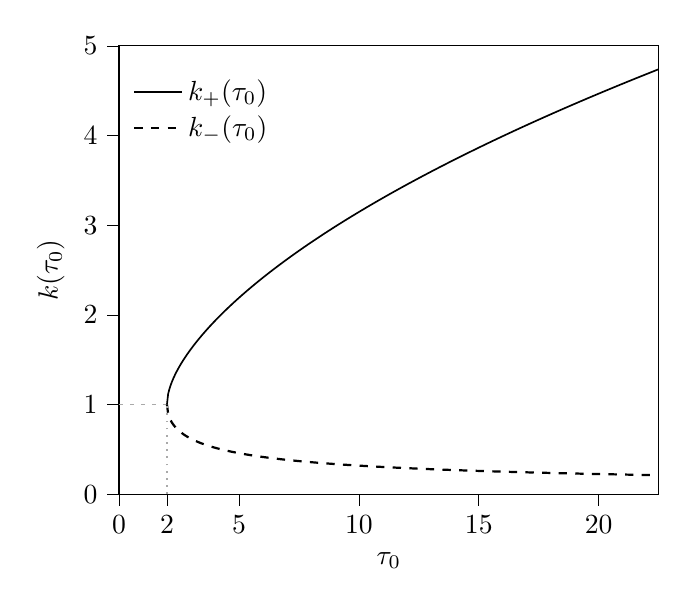
\begin{tikzpicture}

\definecolor{darkgray}{RGB}{169,169,169}
\definecolor{darkgray176}{RGB}{176,176,176}

\begin{axis}[
legend cell align={left},
legend style={
  fill opacity=0.8,
  draw opacity=1,
  text opacity=1,
  at={(0.01,0.95)},
  anchor=north west,
  draw=none
},
tick align=outside,
tick pos=left,
x grid style={darkgray176},
xlabel={\(\displaystyle \tau_0\)},
xmin=0, xmax=22.5,
xtick style={color=black},
y grid style={darkgray176},
ylabel={\(\displaystyle k(\tau_0)\)},
ymin=0, ymax=5,
ytick style={color=black},
xtick={0,2,5,10,15,20}, %afegit a ma
]
\path [draw=darkgray, semithick, dash pattern=on 1.5pt off 2.475pt]
(axis cs:0,1)
--(axis cs:2,1);

\addplot [semithick, black]
table {%
2 1
2.04902451225613 1.1168168000538
2.09804902451226 1.16874583266948
2.14707353676838 1.20996907879261
2.19609804902451 1.24563377354352
2.24512256128064 1.27773402875366
2.29414707353677 1.30729283131175
2.3431715857929 1.33491811026942
2.39219609804902 1.36100615291813
2.44122061030515 1.38583237958527
2.49024512256128 1.40959745757456
2.53926963481741 1.43245299190741
2.58829414707354 1.45451686745395
2.63731865932966 1.47588292272881
2.68634317158579 1.4966273225024
2.73536768384192 1.51681290987781
2.78439219609805 1.53649226973201
2.83341670835418 1.55570994132093
2.88244122061031 1.57450405222229
2.93146573286643 1.59290754851231
2.98049024512256 1.6109491368331
3.02951475737869 1.62865401678076
3.07853926963482 1.64604445799406
3.12756378189095 1.66314026040202
3.17658829414707 1.67995912531485
3.2256128064032 1.6965169576089
3.27463731865933 1.71282811403396
3.32366183091546 1.72890560894476
3.37268634317159 1.74476128605844
3.42171085542771 1.76040596285836
3.47073536768384 1.7758495527916
3.51975987993997 1.7911011693001
3.5687843921961 1.80616921488456
3.61780890445223 1.82106145775459
3.66683341670835 1.83578509811914
3.71585792896448 1.85034682578112
3.76488244122061 1.86475287039304
3.81390695347674 1.87900904548718
3.86293146573287 1.89312078719927
3.91195597798899 1.90709318844842
3.96098049024512 1.92093102920989
4.01000500250125 1.93463880341415
4.05902951475738 1.94822074292179
4.10805402701351 1.96168083895465
4.15707853926963 1.97502286130634
4.20610305152576 1.9882503756078
4.25512756378189 2.00136675888408
4.30415207603802 2.01437521360519
4.35317658829415 2.02727878040605
4.40220110055028 2.04008034962708
4.4512256128064 2.05278267180669
4.50025012506253 2.06538836724035
4.54927463731866 2.07789993470606
4.59829914957479 2.09031975944381
4.64732366183092 2.10265012046582
4.69634817408704 2.1148931972653
4.74537268634317 2.12705107598339
4.7943971985993 2.13912575508701
4.84342171085543 2.1511191506046
4.89244622311156 2.16303310096118
4.94147073536768 2.17486937144995
4.99049524762381 2.18662965837327
5.03951975987994 2.1983155928828
5.08854427213607 2.20992874454508
5.1375687843922 2.2214706246564
5.18659329664832 2.23294268932838
5.23561780890445 2.24434634236324
5.28464232116058 2.25568293793647
5.33366683341671 2.26695378310226
5.38269134567284 2.27816014013605
5.43171585792896 2.28930322872706
5.48074037018509 2.30038422803232
5.52976488244122 2.31140427860305
5.57878939469735 2.32236448419282
5.62781390695348 2.33326591345642
5.6768384192096 2.34410960154752
5.72586293146573 2.35489655162227
5.77488744372186 2.36562773625579
5.82391195597799 2.37630409877755
5.87293646823412 2.3869265545314
5.92196098049024 2.39749599206528
5.97098549274637 2.40801327425561
6.0200100050025 2.41847923937048
6.06903451725863 2.42889470207591
6.11805902951476 2.43926045438882
6.16708354177088 2.4495772665801
6.21610805402701 2.45984588803105
6.26513256628314 2.47006704804607
6.31415707853927 2.48024145662443
6.3631815907954 2.49036980519346
6.41220610305153 2.50045276730567
6.46123061530765 2.51049099930194
6.51025512756378 2.52048514094273
6.55927963981991 2.53043581600925
6.60830415207604 2.54034363287636
6.65732866433217 2.55020918505876
6.70635317658829 2.56003305173204
6.75537768884442 2.56981579822999
6.80440220110055 2.57955797651951
6.85342671335668 2.58926012565431
6.90245122561281 2.59892277220866
6.95147573786893 2.60854643069214
7.00050025012506 2.61813160394645
7.04952476238119 2.62767878352532
7.09854927463732 2.63718845005828
7.14757378689345 2.64666107359917
7.19659829914957 2.65609711396024
7.2456228114057 2.66549702103244
7.29464732366183 2.67486123509276
7.34367183591796 2.68419018709908
7.39269634817409 2.69348429897337
7.44172086043022 2.70274398387356
7.49074537268634 2.71196964645484
7.53976988494247 2.72116168312081
7.5887943971986 2.73032048226496
7.63781890945473 2.73944642450289
7.68684342171086 2.74853988289588
7.73586793396698 2.757601223166
7.78489244622311 2.76663080390324
7.83391695847924 2.77562897676507
7.88294147073537 2.78459608666872
7.9319659829915 2.79353247197648
7.98099049524762 2.80243846467435
8.03001500750375 2.81131439054445
8.07903951975988 2.82016056933119
8.12806403201601 2.82897731490179
8.17708854427214 2.83776493540115
8.22611305652826 2.84652373340145
8.27513756878439 2.8552540060466
8.32416208104052 2.86395604519186
8.37318659329665 2.87263013753877
8.42221110555278 2.88127656476555
8.4712356178089 2.88989560365325
8.52026013006503 2.89848752620777
8.56928464232116 2.90705259977786
8.61830915457729 2.91559108716938
8.66733366683342 2.92410324675588
8.71635817908954 2.93258933258568
8.76538269134567 2.94104959448555
8.8144072036018 2.94948427816118
8.86343171585793 2.95789362529454
8.91245622811406 2.96627787363819
8.96148074037018 2.97463725710679
9.01050525262631 2.98297200586572
9.05952976488244 2.99128234641717
9.10855427713857 2.99956850168352
9.1575787893947 3.00783069108833
9.20660330165083 3.01606913063491
9.25562781390695 3.02428403298259
9.30465232616308 3.03247560752082
9.35367683841921 3.040644060441
9.40270135067534 3.04878959480644
9.45172586293146 3.05691241062016
9.50075037518759 3.06501270489085
9.54977488744372 3.07309067169698
9.59879939969985 3.0811465022491
9.64782391195598 3.08918038495044
9.69684842421211 3.09719250545576
9.74587293646823 3.10518304672873
9.79489744872436 3.11315218909761
9.84392196098049 3.12110011030954
9.89294647323662 3.12902698558328
9.94197098549275 3.13693298766059
9.99099549774887 3.14481828685628
10.040020010005 3.15268305110689
10.0890445222611 3.16052744601809
10.1380690345173 3.16835163491091
10.1870935467734 3.17615577886673
10.2361180590295 3.18394003677112
10.2851425712856 3.19170456535655
10.3341670835418 3.19944951924407
10.3831915957979 3.20717505098388
10.432216108054 3.2148813110949
10.4812406203102 3.22256844810339
10.5302651325663 3.23023660858055
10.5792896448224 3.23788593717925
10.6283141570785 3.24551657666985
10.6773386693347 3.25312866797512
10.7263631815908 3.26072235020434
10.7753876938469 3.26829776068659
10.8244122061031 3.27585503500321
10.8734367183592 3.28339430701955
10.9224612306153 3.29091570891586
10.9714857428714 3.29841937121759
11.0205102551276 3.30590542282488
11.0695347673837 3.31337399104141
11.1185592796398 3.32082520160256
11.1675837918959 3.32825917870295
11.2166083041521 3.33567604502334
11.2656328164082 3.34307592175691
11.3146573286643 3.35045892863492
11.3636818409205 3.3578251839519
11.4127063531766 3.3651748045901
11.4617308654327 3.37250790604358
11.5107553776888 3.37982460244165
11.559779889945 3.38712500657181
11.6088044022011 3.39440922990226
11.6578289144572 3.4016773826038
11.7068534267134 3.40892957357135
11.7558779389695 3.41616591044498
11.8049024512256 3.4233864996305
11.8539269634817 3.43059144631954
11.9029514757379 3.43778085450933
11.951975987994 3.44495482702193
12.0010005002501 3.45211346552317
12.0500250125063 3.45925687054109
12.0990495247624 3.4663851414841
12.1480740370185 3.47349837665866
12.1970985492746 3.4805966732867
12.2461230615308 3.48768012752257
12.2951475737869 3.49474883446977
12.344172086043 3.50180288819721
12.3931965982991 3.50884238175527
12.4422211105553 3.51586740719142
12.4912456228114 3.52287805556561
12.5402701350675 3.52987441696531
12.5892946473237 3.53685658052027
12.6383191595798 3.54382463441699
12.6873436718359 3.55077866591289
12.736368184092 3.55771876135023
12.7853926963482 3.56464500616972
12.8344172086043 3.57155748492391
12.8834417208604 3.57845628129027
12.9324662331166 3.58534147808411
12.9814907453727 3.59221315727111
13.0305152576288 3.59907139997977
13.0795397698849 3.6059162865135
13.1285642821411 3.61274789636255
13.1775887943972 3.6195663082157
13.2266133066533 3.62637159997171
13.2756378189095 3.63316384875062
13.3246623311656 3.63994313090473
13.3736868434217 3.6467095220295
13.4227113556778 3.65346309697418
13.471735867934 3.66020392985223
13.5207603801901 3.66693209405163
13.5697848924462 3.67364766224492
13.6188094047024 3.68035070639908
13.6678339169585 3.6870412977853
13.7168584292146 3.69371950698847
13.7658829414707 3.70038540391655
13.8149074537269 3.70703905780982
13.863931965983 3.71368053724986
13.9129564782391 3.7203099101685
13.9619809904952 3.72692724385649
14.0110055027514 3.73353260497212
14.0600300150075 3.74012605954959
14.1090545272636 3.74670767300736
14.1580790395198 3.75327751015623
14.2071035517759 3.75983563520737
14.256128064032 3.76638211178018
14.3051525762881 3.77291700290999
14.3541770885443 3.7794403710557
14.4032016008004 3.78595227810721
14.4522261130565 3.79245278539277
14.5012506253127 3.79894195368622
14.5502751375688 3.80541984321408
14.5992996498249 3.81188651366252
14.648324162081 3.81834202418423
14.6973486743372 3.82478643340518
14.7463731865933 3.83121979943125
14.7953976988494 3.83764217985479
14.8444222111056 3.84405363176099
14.8934467233617 3.85045421173429
14.9424712356178 3.85684397586449
14.9914957478739 3.86322297975297
15.0405202601301 3.86959127851865
15.0895447723862 3.87594892680393
15.1385692846423 3.88229597878054
15.1875937968984 3.88863248815525
15.2366183091546 3.89495850817553
15.2856428214107 3.9012740916351
15.3346673336668 3.90757929087943
15.383691845923 3.91387415781108
15.4327163581791 3.92015874389504
15.4817408704352 3.92643310016392
15.5307653826913 3.93269727722313
15.5797898949475 3.93895132525587
15.6288144072036 3.9451952940282
15.6778389194597 3.95142923289386
15.7268634317159 3.95765319079916
15.775887943972 3.96386721628771
15.8249124562281 3.97007135750512
15.8739369684842 3.97626566220359
15.9229614807404 3.98245017774648
15.9719859929965 3.98862495111279
16.0210105052526 3.99479002890153
16.0700350175088 4.00094545733612
16.1190595297649 4.00709128226863
16.168084042021 4.01322754918401
16.2171085542771 4.01935430320424
16.2661330665333 4.02547158909245
16.3151575787894 4.03157945125691
16.3641820910455 4.03767793375503
16.4132066033017 4.04376708029729
16.4622311155578 4.04984693425107
16.5112556278139 4.05591753864449
16.56028014007 4.06197893617012
16.6093046523262 4.06803116918871
16.6583291645823 4.07407427973283
16.7073536768384 4.08010830951045
16.7563781890945 4.08613329990849
16.8054027013507 4.09214929199628
16.8544272136068 4.09815632652907
16.9034517258629 4.10415444395136
16.9524762381191 4.11014368440028
17.0015007503752 4.11612408770885
17.0505252626313 4.12209569340931
17.0995497748874 4.12805854073625
17.1485742871436 4.1340126686298
17.1975987993997 4.13995811573876
17.2466233116558 4.1458949204237
17.295647823912 4.15182312075994
17.3446723361681 4.15774275454056
17.3936968484242 4.16365385927942
17.4427213606803 4.16955647221396
17.4917458729365 4.17545063030817
17.5407703851926 4.18133637025538
17.5897948974487 4.18721372848107
17.6388194097049 4.19308274114561
17.687843921961 4.19894344414704
17.7368684342171 4.20479587312366
17.7858929464732 4.21064006345679
17.8349174587294 4.21647605027331
17.8839419709855 4.22230386844826
17.9329664832416 4.2281235526074
17.9819909954977 4.23393513712973
18.0310155077539 4.23973865614995
18.08004002001 4.24553414356091
18.1290645322661 4.25132163301605
18.1780890445223 4.25710115793177
18.2271135567784 4.26287275148978
18.2761380690345 4.26863644663945
18.3251625812906 4.27439227610007
18.3741870935468 4.28014027236314
18.4232116058029 4.28588046769461
18.472236118059 4.29161289413708
18.5212606303152 4.29733758351196
18.5702851425713 4.30305456742167
18.6193096548274 4.30876387725174
18.6683341670835 4.31446554417288
18.7173586793397 4.32015959914312
18.7663831915958 4.32584607290979
18.8154077038519 4.33152499601159
18.8644322161081 4.33719639878056
18.9134567283642 4.34286031134405
18.9624812406203 4.3485167636267
19.0115057528764 4.35416578535232
19.0605302651326 4.35980740604582
19.1095547773887 4.36544165503508
19.1585792896448 4.37106856145279
19.207603801901 4.3766881542383
19.2566283141571 4.38230046213941
19.3056528264132 4.38790551371418
19.3546773386693 4.39350333733269
19.4037018509255 4.39909396117875
19.4527263631816 4.40467741325167
19.5017508754377 4.41025372136795
19.5507753876938 4.41582291316295
19.59979989995 4.42138501609254
19.6488244122061 4.42694005743478
19.6978489244622 4.43248806429152
19.7468734367184 4.43802906359001
19.7958979489745 4.44356308208448
19.8449224612306 4.4490901463577
19.8939469734867 4.45461028282256
19.9429714857429 4.46012351772356
19.991995997999 4.46562987713834
20.0410205102551 4.47112938697918
20.0900450225113 4.47662207299448
20.1390695347674 4.4821079607702
20.1880940470235 4.48758707573131
20.2371185592796 4.49305944314325
20.2861430715358 4.49852508811328
20.3351675837919 4.50398403559193
20.384192096048 4.50943631037436
20.4332166083041 4.51488193710169
20.4822411205603 4.52032094026241
20.5312656328164 4.52575334419366
20.5802901450725 4.53117917308257
20.6293146573287 4.53659845096756
20.6783391695848 4.54201120173963
20.7273636818409 4.54741744914362
20.776388194097 4.55281721677948
20.8254127063532 4.55821052810353
20.8744372186093 4.56359740642964
20.9234617308654 4.56897787493052
20.9724862431216 4.57435195663887
21.0215107553777 4.57971967444857
21.0705352676338 4.58508105111592
21.1195597798899 4.59043610926071
21.1685842921461 4.59578487136746
21.2176088044022 4.60112735978649
21.2666333166583 4.60646359673511
21.3156578289145 4.61179360429869
21.3646823411706 4.61711740443177
21.4137068534267 4.62243501895916
21.4627313656828 4.62774646957703
21.511755877939 4.63305177785395
21.5607803901951 4.63835096523197
21.6098049024512 4.64364405302764
21.6588294147074 4.64893106243308
21.7078539269635 4.65421201451696
21.7568784392196 4.65948693022556
21.8059029514757 4.66475583038372
21.8549274637319 4.67001873569587
21.903951975988 4.67527566674698
21.9529764882441 4.68052664400357
22.0020010005003 4.68577168781461
22.0510255127564 4.69101081841255
22.1000500250125 4.69624405591416
22.1490745372686 4.70147142032156
22.1980990495248 4.70669293152307
22.2471235617809 4.71190860929416
22.296148074037 4.71711847329831
22.3451725862931 4.72232254308796
22.3941970985493 4.72752083810534
22.4432216108054 4.73271337768337
22.4922461230615 4.73790018104651
22.5412706353177 4.74308126731165
22.5902951475738 4.74825665548891
22.6393196598299 4.75342636448251
22.688344172086 4.75859041309158
22.7373686843422 4.76374882001102
22.7863931965983 4.76890160383226
22.8354177088544 4.77404878304409
22.8844422211106 4.77919037603349
22.9334667333667 4.78432640108635
22.9824912456228 4.78945687638831
23.0315157578789 4.79458182002551
23.0805402701351 4.79970124998535
23.1295647823912 4.80481518415728
23.1785892946473 4.80992364033349
23.2276138069035 4.81502663620972
23.2766383191596 4.82012418938594
23.3256628314157 4.82521631736714
23.3746873436718 4.83030303756399
23.423711855928 4.83538436729358
23.4727363681841 4.84046032378013
23.5217608804402 4.8455309241557
23.5707853926963 4.85059618546086
23.6198099049525 4.8556561246454
23.6688344172086 4.86071075856897
23.7178589294647 4.86576010400183
23.7668834417209 4.87080417762542
23.815907953977 4.8758429960331
23.8649324662331 4.88087657573077
23.9139569784892 4.88590493313753
23.9629814907454 4.89092808458629
24.0120060030015 4.89594604632446
24.0610305152576 4.90095883451453
24.1100550275138 4.90596646523472
24.1590795397699 4.9109689544796
24.208104052026 4.91596631816068
24.2571285642821 4.92095857210705
24.3061530765383 4.92594573206594
24.3551775887944 4.93092781370334
24.4042021010505 4.9359048326046
24.4532266133067 4.94087680427498
24.5022511255628 4.94584374414025
24.5512756378189 4.95080566754728
24.600300150075 4.95576258976456
24.6493246623312 4.96071452598281
24.6983491745873 4.9656614913155
24.7473736868434 4.97060350079943
24.7963981990995 4.97554056939527
24.8454227113557 4.98047271198808
24.8944472236118 4.98539994338788
24.9434717358679 4.99032227833017
24.9924962481241 4.99523973147643
25.0415207603802 5.00015231741469
25.0905452726363 5.00506005066001
25.1395697848924 5.00996294565501
25.1885942971486 5.01486101677038
25.2376188094047 5.01975427830537
25.2866433216608 5.02464274448829
25.335667833917 5.02952642947703
25.3846923461731 5.03440534735951
25.4337168584292 5.03927951215422
25.4827413706853 5.04414893781062
25.5317658829415 5.04901363820971
25.5807903951976 5.05387362716444
25.6298149074537 5.05872891842019
25.6788394197099 5.06357952565524
25.727863931966 5.06842546248125
25.7768884442221 5.07326674244369
25.8259129564782 5.07810337902228
25.8749374687344 5.08293538563149
25.9239619809905 5.08776277562093
25.9729864932466 5.09258556227581
26.0220110055028 5.0974037588174
26.0710355177589 5.10221737840342
26.120060030015 5.10702643412851
26.1690845422711 5.1118309390246
26.2181090545273 5.11663090606142
26.2671335667834 5.12142634814682
26.3161580790395 5.12621727812725
26.3651825912956 5.13100370878814
26.4142071035518 5.13578565285433
26.4632316158079 5.14056312299044
26.512256128064 5.14533613180131
26.5612806403202 5.15010469183237
26.6103051525763 5.15486881557004
26.6593296648324 5.15962851544211
26.7083541770885 5.16438380381815
26.7573786893447 5.16913469300988
26.8064032016008 5.17388119527155
26.8554277138569 5.1786233228003
26.9044522261131 5.18336108773658
26.9534767383692 5.18809450216446
27.0025012506253 5.19282357811205
27.0515257628814 5.19754832755184
27.1005502751376 5.20226876240105
27.1495747873937 5.20698489452202
27.1985992996498 5.21169673572253
27.247623811906 5.21640429775619
27.2966483241621 5.22110759232276
27.3456728364182 5.22580663106849
27.3946973486743 5.23050142558649
27.4437218609305 5.23519198741708
27.4927463731866 5.23987832804807
27.5417708854427 5.24456045891517
27.5907953976988 5.24923839140224
27.639819909955 5.25391213684172
27.6888444222111 5.25858170651484
27.7378689344672 5.26324711165206
27.7868934467234 5.26790836343331
27.8359179589795 5.27256547298833
27.8849424712356 5.277218451397
27.9339669834917 5.28186730968966
27.9829914957479 5.28651205884739
28.032016008004 5.29115270980235
28.0810405202601 5.29578927343804
28.1300650325163 5.30042176058968
28.1790895447724 5.30505018204444
28.2281140570285 5.30967454854177
28.2771385692846 5.31429487077369
28.3261630815408 5.3189111593851
28.3751875937969 5.32352342497405
28.424212106053 5.32813167809203
28.4732366183092 5.33273592924428
28.5222611305653 5.33733618889004
28.5712856428214 5.34193246744288
28.6203101550775 5.34652477527092
28.6693346673337 5.35111312269717
28.7183591795898 5.35569751999976
28.7673836918459 5.36027797741223
28.816408204102 5.36485450512382
28.8654327163582 5.36942711327969
28.9144572286143 5.37399581198124
28.9634817408704 5.37856061128636
29.0125062531266 5.38312152120967
29.0615307653827 5.38767855172281
29.1105552776388 5.39223171275468
29.1595797898949 5.39678101419171
29.2086043021511 5.40132646587811
29.2576288144072 5.40586807761611
29.3066533266633 5.41040585916624
29.3556778389195 5.41493982024756
29.4047023511756 5.41946997053791
29.4537268634317 5.42399631967414
29.5027513756878 5.42851887725239
29.551775887944 5.4330376528283
29.6008004002001 5.43755265591727
29.6498249124562 5.44206389599467
29.6988494247124 5.44657138249613
29.7478739369685 5.4510751248177
29.7968984492246 5.45557513231614
29.8459229614807 5.46007141430913
29.8949474737369 5.46456398007552
29.943971985993 5.4690528388555
29.9929964982491 5.47353799985089
30.0420210105053 5.47801947222535
30.0910455227614 5.48249726510456
30.1400700350175 5.4869713875765
30.1890945472736 5.49144184869163
30.2381190595298 5.4959086574631
30.2871435717859 5.50037182286701
30.336168084042 5.50483135384259
30.3851925962981 5.50928725929241
30.4342171085543 5.5137395480826
30.4832416208104 5.51818822904309
30.5322661330665 5.52263331096774
30.5812906453227 5.52707480261464
30.6303151575788 5.53151271270623
30.6793396698349 5.53594704992957
30.728364182091 5.54037782293651
30.7773886943472 5.54480504034387
30.8264132066033 5.5492287107337
30.8754377188594 5.55364884265341
30.9244622311156 5.558065444616
30.9734867433717 5.56247852510027
31.0225112556278 5.56688809255098
31.0715357678839 5.57129415537905
31.1205602801401 5.57569672196176
31.1695847923962 5.58009580064293
31.2186093046523 5.58449139973313
31.2676338169085 5.58888352750982
31.3166583291646 5.59327219221759
31.3656828414207 5.5976574020683
31.4147073536768 5.60203916524127
31.463731865933 5.60641748988349
31.5127563781891 5.61079238410976
31.5617808904452 5.61516385600291
31.6108054027013 5.61953191361392
31.6598299149575 5.62389656496216
31.7088544272136 5.62825781803553
31.7578789394697 5.63261568079061
31.8069034517259 5.63697016115289
31.855927963982 5.6413212670169
31.9049524762381 5.64566900624639
31.9539769884942 5.65001338667449
32.0030015007504 5.6543544161039
32.0520260130065 5.65869210230702
32.1010505252626 5.66302645302616
32.1500750375188 5.66735747597367
32.1990995497749 5.6716851788321
32.248124062031 5.6760095692544
32.2971485742871 5.68033065486403
32.3461730865433 5.68464844325515
32.3951975987994 5.68896294199277
32.4442221110555 5.69327415861292
32.4932466233117 5.69758210062279
32.5422711355678 5.70188677550087
32.5912956478239 5.70618819069715
32.64032016008 5.71048635363322
32.6893446723362 5.71478127170247
32.7383691845923 5.71907295227021
32.7873936968484 5.72336140267381
32.8364182091046 5.72764663022288
32.8854427213607 5.73192864219942
32.9344672336168 5.73620744585791
32.9834917458729 5.74048304842553
33.0325162581291 5.74475545710225
33.0815407703852 5.74902467906101
33.1305652826413 5.75329072144782
33.1795897948975 5.75755359138194
33.2286143071536 5.76181329595603
33.2776388194097 5.76606984223623
33.3266633316658 5.77032323726235
33.375687843922 5.77457348804801
33.4247123561781 5.77882060158073
33.4737368684342 5.78306458482213
33.5227613806903 5.787305444708
33.5717858929465 5.7915431881485
33.6208104052026 5.79577782202822
33.6698349174587 5.80000935320637
33.7188594297149 5.80423778851691
33.767883941971 5.80846313476864
33.8169084542271 5.81268539874536
33.8659329664832 5.81690458720598
33.9149574787394 5.82112070688468
33.9639819909955 5.82533376449101
34.0130065032516 5.82954376671001
34.0620310155078 5.83375072020238
34.1110555277639 5.83795463160452
34.16008004002 5.84215550752877
34.2091045522761 5.84635335456342
34.2581290645323 5.85054817927291
34.3071535767884 5.85473998819791
34.3561780890445 5.85892878785546
34.4052026013007 5.86311458473908
34.4542271135568 5.8672973853189
34.5032516258129 5.87147719604176
34.552276138069 5.87565402333135
34.6013006503252 5.87982787358831
34.6503251625813 5.88399875319036
34.6993496748374 5.88816666849238
34.7483741870935 5.89233162582658
34.7973986993497 5.89649363150257
34.8464232116058 5.90065269180749
34.8954477238619 5.90480881300612
34.9444722361181 5.908962001341
34.9934967483742 5.91311226303251
35.0425212606303 5.91725960427903
35.0915457728864 5.92140403125701
35.1405702851426 5.92554555012107
35.1895947973987 5.92968416700416
35.2386193096548 5.93381988801762
35.287643821911 5.93795271925131
35.3366683341671 5.94208266677369
35.3856928464232 5.94620973663197
35.4347173586793 5.95033393485217
35.4837418709355 5.95445526743923
35.5327663831916 5.95857374037717
35.5817908954477 5.9626893596291
35.6308154077038 5.9668021311374
35.67983991996 5.97091206082377
35.7288644322161 5.97501915458938
35.7778889444722 5.97912341831491
35.8269134567284 5.9832248578607
35.8759379689845 5.98732347906683
35.9249624812406 5.99141928775322
35.9739869934967 5.99551228971972
36.0230115057529 5.9996024907462
36.072036018009 6.0036898965927
36.1210605302651 6.00777451299944
36.1700850425213 6.01185634568699
36.2191095547774 6.01593540035633
36.2681340670335 6.02001168268894
36.3171585792896 6.02408519834691
36.3661830915458 6.02815595297301
36.4152076038019 6.03222395219083
36.464232116058 6.03628920160482
36.5132566283142 6.04035170680038
36.5622811405703 6.04441147334402
36.6113056528264 6.04846850678335
36.6603301650825 6.05252281264727
36.7093546773387 6.05657439644596
36.7583791895948 6.06062326367105
36.8074037018509 6.06466941979568
36.8564282141071 6.06871287027456
36.9054527263632 6.0727536205441
36.9544772386193 6.07679167602245
37.0035017508754 6.08082704210966
37.0525262631316 6.08485972418766
37.1015507753877 6.08888972762045
37.1505752876438 6.0929170577541
37.1995997998999 6.0969417199169
37.2486243121561 6.10096371941939
37.2976488244122 6.10498306155448
37.3466733366683 6.10899975159751
37.3956978489245 6.11301379480635
37.4447223611806 6.11702519642145
37.4937468734367 6.12103396166597
37.5427713856928 6.1250400957458
37.591795897949 6.12904360384971
37.6408204102051 6.13304449114936
37.6898449224612 6.13704276279941
37.7388694347174 6.14103842393762
37.7878939469735 6.14503147968489
37.8369184592296 6.14902193514536
37.8859429714857 6.15300979540647
37.9349674837419 6.15699506553906
37.983991995998 6.16097775059743
38.0330165082541 6.1649578556194
38.0820410205103 6.16893538562644
38.1310655327664 6.17291034562368
38.1800900450225 6.17688274060001
38.2291145572786 6.18085257552818
38.2781390695348 6.18481985536484
38.3271635817909 6.18878458505061
38.376188094047 6.19274676951018
38.4252126063031 6.19670641365235
38.4742371185593 6.20066352237016
38.5232616308154 6.20461810054087
38.5722861430715 6.20857015302611
38.6213106553277 6.21251968467192
38.6703351675838 6.21646670030881
38.7193596798399 6.22041120475186
38.7683841920961 6.22435320280076
38.8174087043522 6.22829269923989
38.8664332166083 6.23222969883839
38.9154577288644 6.23616420635023
38.9644822411206 6.24009622651426
39.0135067533767 6.2440257640543
39.0625312656328 6.24795282367922
39.1115557778889 6.25187741008294
39.1605802901451 6.25579952794457
39.2096048024012 6.25971918192846
39.2586293146573 6.26363637668421
39.3076538269135 6.26755111684681
39.3566783391696 6.27146340703667
39.4057028514257 6.27537325185967
39.4547273636818 6.27928065590725
39.503751875938 6.28318562375646
39.5527763881941 6.28708815997004
39.6018009004502 6.29098826909644
39.6508254127064 6.29488595566994
39.6998499249625 6.29878122421067
39.7488744372186 6.30267407922469
39.7978989494747 6.30656452520404
39.8469234617309 6.31045256662683
39.895947973987 6.31433820795726
39.9449724862431 6.31822145364569
39.9939969984992 6.32210230812874
40.0430215107554 6.3259807758293
40.0920460230115 6.32985686115659
40.1410705352676 6.33373056850629
40.1900950475238 6.33760190226049
40.2391195597799 6.34147086678784
40.288144072036 6.34533746644356
40.3371685842921 6.34920170556952
40.3861930965483 6.35306358849427
40.4352176088044 6.35692311953313
40.4842421210605 6.36078030298824
40.5332666333167 6.36463514314858
40.5822911455728 6.36848764429008
40.6313156578289 6.37233781067564
40.680340170085 6.37618564655521
40.7293646823412 6.3800311561658
40.7783891945973 6.38387434373159
40.8274137068534 6.38771521346397
40.8764382191096 6.39155376956157
40.9254627313657 6.39539001621032
40.9744872436218 6.39922395758353
41.0235117558779 6.40305559784192
41.0725362681341 6.40688494113369
41.1215607803902 6.41071199159454
41.1705852926463 6.41453675334777
41.2196098049024 6.41835923050429
41.2686343171586 6.4221794271627
41.3176588294147 6.42599734740933
41.3666833416708 6.42981299531829
41.415707853927 6.43362637495152
41.4647323661831 6.43743749035885
41.5137568784392 6.44124634557804
41.5627813906953 6.44505294463486
41.6118059029515 6.44885729154308
41.6608304152076 6.45265939030458
41.7098549274637 6.45645924490936
41.7588794397199 6.46025685933562
41.807903951976 6.46405223754979
41.8569284642321 6.46784538350657
41.9059529764882 6.47163630114901
41.9549774887444 6.47542499440853
42.0040020010005 6.47921146720497
42.0530265132566 6.48299572344665
42.1020510255128 6.48677776703043
42.1510755377689 6.49055760184171
42.200100050025 6.49433523175452
42.2491245622811 6.49811066063157
42.2981490745373 6.50188389232425
42.3471735867934 6.50565493067273
42.3961980990495 6.50942377950597
42.4452226113057 6.51319044264178
42.4942471235618 6.51695492388687
42.5432716358179 6.52071722703688
42.592296148074 6.52447735587643
42.6413206603302 6.52823531417919
42.6903451725863 6.53199110570788
42.7393696848424 6.53574473421435
42.7883941970985 6.5394962034396
42.8374187093547 6.54324551711386
42.8864432216108 6.54699267895659
42.9354677338669 6.55073769267653
42.9844922461231 6.55448056197179
43.0335167583792 6.55822129052983
43.0825412706353 6.56195988202754
43.1315657828914 6.56569634013129
43.1805902951476 6.56943066849693
43.2296148074037 6.57316287076987
43.2786393196598 6.57689295058511
43.327663831916 6.5806209115673
43.3766883441721 6.58434675733073
43.4257128564282 6.58807049147942
43.4747373686843 6.59179211760715
43.5237618809405 6.5955116392975
43.5727863931966 6.59922906012388
43.6218109054527 6.60294438364956
43.6708354177089 6.60665761342777
43.719859929965 6.61036875300165
43.7688844422211 6.61407780590438
43.8179089544772 6.61778477565914
43.8669334667334 6.62148966577921
43.9159579789895 6.62519247976799
43.9649824912456 6.628893221119
44.0140070035018 6.632591893316
44.0630315157579 6.63628849983295
44.112056028014 6.63998304413408
44.1610805402701 6.64367552967394
44.2101050525263 6.64736595989743
44.2591295647824 6.65105433823983
44.3081540770385 6.65474066812682
44.3571785892946 6.65842495297458
44.4062031015508 6.66210719618975
44.4552276138069 6.66578740116953
44.504252126063 6.66946557130167
44.5532766383192 6.67314170996453
44.6023011505753 6.67681582052714
44.6513256628314 6.68048790634916
44.7003501750875 6.68415797078102
44.7493746873437 6.68782601716386
44.7983991995998 6.69149204882963
44.8474237118559 6.6951560691011
44.8964482241121 6.69881808129189
44.9454727363682 6.70247808870653
44.9944972486243 6.70613609464045
45.0435217608804 6.70979210238008
45.0925462731366 6.71344611520283
45.1415707853927 6.71709813637713
45.1905952976488 6.72074816916251
45.239619809905 6.72439621680957
45.2886443221611 6.72804228256006
45.3376688344172 6.73168636964691
45.3866933466733 6.73532848129423
45.4357178589295 6.73896862071738
45.4847423711856 6.742606791123
45.5337668834417 6.74624299570901
45.5827913956978 6.74987723766468
45.631815907954 6.75350952017066
45.6808404202101 6.75713984639897
45.7298649324662 6.76076821951311
45.7788894447224 6.764394642668
45.8279139569785 6.76801911901009
45.8769384692346 6.77164165167735
45.9259629814907 6.77526224379932
45.9749874937469 6.77888089849712
46.024012006003 6.78249761888353
46.0730365182591 6.78611240806294
46.1220610305153 6.78972526913148
46.1710855427714 6.79333620517695
46.2201100550275 6.79694521927895
46.2691345672836 6.80055231450882
46.3181590795398 6.80415749392976
46.3671835917959 6.80776076059676
46.416208104052 6.81136211755673
46.4652326163081 6.81496156784845
46.5142571285643 6.81855911450267
46.5632816408204 6.82215476054207
46.6123061530765 6.82574850898135
46.6613306653327 6.82934036282722
46.7103551775888 6.83293032507845
46.7593796898449 6.83651839872589
46.8084042021011 6.8401045867525
46.8574287143572 6.84368889213339
46.9064532266133 6.84727131783584
46.9554777388694 6.85085186681933
47.0045022511256 6.85443054203554
47.0535267633817 6.85800734642846
47.1025512756378 6.86158228293432
47.1515757878939 6.86515535448168
47.2006003001501 6.86872656399144
47.2496248124062 6.87229591437688
47.2986493246623 6.87586340854367
47.3476738369185 6.8794290493899
47.3966983491746 6.88299283980611
47.4457228614307 6.88655478267535
47.4947473736868 6.89011488087313
47.543771885943 6.89367313726755
47.5927963981991 6.89722955471923
47.6418209104552 6.90078413608139
47.6908454227114 6.90433688419989
47.7398699349675 6.90788780191319
47.7888944472236 6.91143689205247
47.8379189594797 6.91498415744156
47.8869434717359 6.91852960089705
47.935967983992 6.92207322522825
47.9849924962481 6.92561503323727
48.0340170085043 6.929155027719
48.0830415207604 6.93269321146118
48.1320660330165 6.93622958724437
48.1810905452726 6.93976415784204
48.2301150575288 6.94329692602055
48.2791395697849 6.9468278945392
48.328164082041 6.95035706615023
48.3771885942971 6.95388444359887
48.4262131065533 6.95741002962335
48.4752376188094 6.96093382695494
48.5242621310655 6.96445583831794
48.5732866433217 6.96797606642977
48.6223111555778 6.97149451400092
48.6713356678339 6.97501118373503
48.72036018009 6.97852607832887
48.7693846923462 6.98203920047242
48.8184092046023 6.98555055284883
48.8674337168584 6.98906013813449
48.9164582291146 6.99256795899905
48.9654827413707 6.99607401810541
49.0145072536268 6.9995783181098
49.0635317658829 7.00308086166173
49.1125562781391 7.00658165140409
49.1615807903952 7.01008068997313
49.2106053026513 7.01357797999847
49.2596298149075 7.01707352410317
49.3086543271636 7.02056732490372
49.3576788394197 7.02405938501006
49.4067033516758 7.02754970702562
49.455727863932 7.03103829354736
49.5047523761881 7.03452514716572
49.5537768884442 7.03801027046474
49.6028014007004 7.041493666022
49.6518259129565 7.0449753364087
49.7008504252126 7.04845528418964
49.7498749374687 7.05193351192327
49.7988994497249 7.05541002216171
49.847923961981 7.05888481745076
49.8969484742371 7.0623579003299
49.9459729864932 7.06582927333239
49.9949974987494 7.06929893898521
50.0440220110055 7.0727668998091
50.0930465232616 7.07623315831862
50.1420710355178 7.07969771702213
50.1910955477739 7.08316057842183
50.24012006003 7.08662174501378
50.2891445722861 7.09008121928792
50.3381690845423 7.09353900372807
50.3871935967984 7.09699510081201
50.4362181090545 7.10044951301141
50.4852426213107 7.10390224279195
50.5342671335668 7.10735329261327
50.5832916458229 7.11080266492901
50.632316158079 7.11425036218684
50.6813406703352 7.11769638682847
50.7303651825913 7.12114074128969
50.7793896948474 7.12458342800035
50.8284142071035 7.12802444938443
50.8774387193597 7.13146380786001
50.9264632316158 7.13490150583934
50.9754877438719 7.13833754572881
51.0245122561281 7.14177192992901
51.0735367683842 7.14520466083474
51.1225612806403 7.14863574083501
51.1715857928964 7.15206517231307
51.2206103051526 7.15549295764644
51.2696348174087 7.15891909920694
51.3186593296648 7.16234359936066
51.367683841921 7.16576646046802
51.4167083541771 7.16918768488379
51.4657328664332 7.1726072749571
51.5147573786893 7.17602523303144
51.5637818909455 7.17944156144471
51.6128064032016 7.18285626252922
51.6618309154577 7.18626933861171
51.7108554277139 7.18968079201339
51.75987993997 7.19309062504992
51.8089044522261 7.19649884003146
51.8579289644822 7.19990543926268
51.9069534767384 7.20331042504276
51.9559779889945 7.20671379966545
52.0050025012506 7.21011556541904
52.0540270135068 7.21351572458642
52.1030515257629 7.21691427944505
52.152076038019 7.22031123226704
52.2011005502751 7.22370658531911
52.2501250625313 7.22710034086264
52.2991495747874 7.23049250115368
52.3481740870435 7.23388306844297
52.3971985992996 7.23727204497595
52.4462231115558 7.24065943299278
52.4952476238119 7.24404523472837
52.544272136068 7.24742945241238
52.5932966483242 7.25081208826924
52.6423211605803 7.25419314451817
52.6913456728364 7.25757262337321
52.7403701850925 7.26095052704322
52.7893946973487 7.26432685773191
52.8384192096048 7.26770161763782
52.8874437218609 7.2710748089544
52.9364682341171 7.27444643386997
52.9854927463732 7.27781649456778
53.0345172586293 7.28118499322599
53.0835417708854 7.28455193201771
53.1325662831416 7.287917313111
53.1815907953977 7.29128113866889
53.2306153076538 7.29464341084944
53.27963981991 7.29800413180566
53.3286643321661 7.30136330368564
53.3776888444222 7.30472092863247
53.4267133566783 7.30807700878431
53.4757378689345 7.3114315462744
53.5247623811906 7.31478454323106
53.5737868934467 7.31813600177771
53.6228114057028 7.32148592403289
53.671835917959 7.32483431211029
53.7208604302151 7.32818116811873
53.7698849424712 7.33152649416221
53.8189094547274 7.33487029233992
53.8679339669835 7.33821256474622
53.9169584792396 7.34155331347071
53.9659829914957 7.3448925405982
54.0150075037519 7.34823024820876
54.064032016008 7.35156643837771
54.1130565282641 7.35490111317564
54.1620810405203 7.35823427466843
54.2111055527764 7.36156592491726
54.2601300650325 7.36489606597866
54.3091545772886 7.36822469990445
54.3581790895448 7.37155182874181
54.4072036018009 7.37487745453332
54.456228114057 7.37820157931688
54.5052526263132 7.38152420512584
54.5542771385693 7.3848453339889
54.6033016508254 7.38816496793023
54.6523261630815 7.39148310896942
54.7013506753377 7.3947997591215
54.7503751875938 7.39811492039697
54.7993996998499 7.40142859480182
54.8484242121061 7.40474078433753
54.8974487243622 7.40805149100107
54.9464732366183 7.41136071678496
54.9954977488744 7.41466846367724
55.0445222611306 7.4179747336615
55.0935467733867 7.42127952871689
55.1425712856428 7.42458285081815
55.1915957978989 7.42788470193561
55.2406203101551 7.43118508403519
55.2896448224112 7.43448399907845
55.3386693346673 7.43778144902256
55.3876938469235 7.44107743582037
55.4367183591796 7.44437196142035
55.4857428714357 7.44766502776668
55.5347673836918 7.45095663679919
55.583791895948 7.45424679045345
55.6328164082041 7.45753549066072
55.6818409204602 7.46082273934798
55.7308654327164 7.46410853843797
55.7798899449725 7.46739288984917
55.8289144572286 7.47067579549584
55.8779389694847 7.47395725728801
55.9269634817409 7.4772372771315
55.975987993997 7.48051585692794
56.0250125062531 7.48379299857477
56.0740370185093 7.48706870396529
56.1230615307654 7.4903429749886
56.1720860430215 7.49361581352971
56.2211105552776 7.49688722146944
56.2701350675338 7.50015720068455
56.3191595797899 7.50342575304765
56.368184092046 7.50669288042728
56.4172086043021 7.50995858468791
56.4662331165583 7.51322286768992
56.5152576288144 7.51648573128963
56.5642821410705 7.51974717733936
56.6133066533267 7.52300720768735
56.6623311655828 7.52626582417786
56.7113556778389 7.52952302865111
56.760380190095 7.53277882294336
56.8094047023512 7.53603320888687
56.8584292146073 7.53928618830993
56.9074537268634 7.54253776303687
56.9564782391196 7.5457879348881
57.0055027513757 7.54903670568007
57.0545272636318 7.55228407722531
57.1035517758879 7.55553005133246
57.1525762881441 7.55877462980624
57.2016008004002 7.5620178144475
57.2506253126563 7.56525960705321
57.2996498249125 7.56850000941647
57.3486743371686 7.57173902332655
57.3976988494247 7.57497665056885
57.4467233616808 7.57821289292497
57.495747873937 7.58144775217268
57.5447723861931 7.58468123008595
57.5937968984492 7.58791332843496
57.6428214107054 7.59114404898609
57.6918459229615 7.59437339350196
57.7408704352176 7.59760136374145
57.7898949474737 7.60082796145966
57.8389194597299 7.60405318840797
57.887943971986 7.60727704633404
57.9369684842421 7.61049953698179
57.9859929964982 7.61372066209146
58.0350175087544 7.61694042339959
58.0840420210105 7.62015882263905
58.1330665332666 7.623375861539
58.1820910455228 7.62659154182499
58.2311155577789 7.62980586521889
58.280140070035 7.63301883343894
58.3291645822911 7.63623044819975
58.3781890945473 7.63944071121232
58.4272136068034 7.64264962418403
58.4762381190595 7.64585718881869
58.5252626313157 7.64906340681649
58.5742871435718 7.65226827987408
58.6233116558279 7.65547180968452
58.672336168084 7.65867399793733
58.7213606803402 7.66187484631849
58.7703851925963 7.66507435651044
58.8194097048524 7.66827253019209
58.8684342171086 7.67146936903886
58.9174587293647 7.67466487472265
58.9664832416208 7.67785904891188
59.0155077538769 7.68105189327148
59.0645322661331 7.68424340946292
59.1135567783892 7.6874335991442
59.1625812906453 7.69062246396986
59.2116058029014 7.69381000559103
59.2606303151576 7.69699622565539
59.3096548274137 7.70018112580718
59.3586793396698 7.70336470768727
59.407703851926 7.70654697293311
59.4567283641821 7.70972792317874
59.5057528764382 7.71290756005486
59.5547773886943 7.71608588518875
59.6038019009505 7.71926290020438
59.6528264132066 7.72243860672233
59.7018509254627 7.72561300635985
59.7508754377189 7.72878610073086
59.799899949975 7.73195789144595
59.8489244622311 7.73512838011242
59.8979489744872 7.73829756833423
59.9469734867434 7.74146545771208
59.9959979989995 7.74463204984336
60.0450225112556 7.74779734632219
60.0940470235118 7.75096134873944
60.1430715357679 7.75412405868271
60.192096048024 7.75728547773635
60.2411205602801 7.76044560748148
60.2901450725363 7.76360444949599
60.3391695847924 7.76676200535455
60.3881940970485 7.76991827662862
60.4372186093047 7.77307326488645
60.4862431215608 7.77622697169312
60.5352676338169 7.77937939861051
60.584292146073 7.78253054719732
60.6333166583292 7.78568041900911
60.6823411705853 7.78882901559825
60.7313656828414 7.79197633851401
60.7803901950975 7.79512238930247
60.8294147073537 7.79826716950663
60.8784392196098 7.80141068066633
60.9274637318659 7.80455292431832
60.9764882441221 7.80769390199624
61.0255127563782 7.81083361523065
61.0745372686343 7.813972065549
61.1235617808904 7.81710925447569
61.1725862931466 7.82024518353204
61.2216108054027 7.8233798542363
61.2706353176588 7.8265132681037
61.319659829915 7.8296454266464
61.3686843421711 7.83277633137354
61.4177088544272 7.83590598379124
61.4667333666833 7.83903438540258
61.5157578789395 7.84216153770766
61.5647823911956 7.84528744220357
61.6138069034517 7.84841210038441
61.6628314157078 7.8515355137413
61.711855927964 7.85465768376237
61.7608804402201 7.8577786119328
61.8099049524762 7.86089829973483
61.8589294647324 7.8640167486477
61.9079539769885 7.86713396014776
61.9569784892446 7.8702499357084
62.0060030015008 7.87336467680009
62.0550275137569 7.87647818489039
62.104052026013 7.87959046144394
62.1530765382691 7.8827015079225
62.2021010505253 7.8858113257849
62.2511255627814 7.88891991648713
62.3001500750375 7.89202728148228
62.3491745872936 7.89513342222057
62.3981990995498 7.89823834014937
62.4472236118059 7.90134203671319
62.496248124062 7.90444451335369
62.5452726363182 7.90754577150971
62.5942971485743 7.91064581261725
62.6433216608304 7.91374463810948
62.6923461730865 7.91684224941678
62.7413706853427 7.91993864796671
62.7903951975988 7.92303383518403
62.8394197098549 7.9261278124907
62.8884442221111 7.92922058130593
62.9374687343672 7.93231214304613
62.9864932466233 7.93540249912494
63.0355177588794 7.93849165095325
63.0845422711356 7.9415795999392
63.1335667833917 7.94466634748817
63.1825912956478 7.94775189500283
63.2316158079039 7.95083624388309
63.2806403201601 7.95391939552615
63.3296648324162 7.9570013513265
63.3786893446723 7.96008211267592
63.4277138569285 7.96316168096348
63.4767383691846 7.96624005757558
63.5257628814407 7.9693172438959
63.5747873936968 7.97239324130548
63.623811905953 7.97546805118265
63.6728364182091 7.97854167490311
63.7218609304652 7.98161411383989
63.7708854427214 7.98468536936336
63.8199099549775 7.98775544284126
63.8689344672336 7.9908243356387
63.9179589794897 7.99389204911814
63.9669834917459 7.99695858463945
64.016008004002 8.00002394355986
64.0650325162581 8.00308812723401
64.1140570285143 8.00615113701392
64.1630815407704 8.00921297424904
64.2121060530265 8.01227364028622
64.2611305652826 8.01533313646974
64.3101550775388 8.0183914641413
64.3591795897949 8.02144862464003
64.408204102051 8.02450461930252
64.4572286143072 8.02755944946279
64.5062531265633 8.03061311645233
64.5552776388194 8.03366562160009
64.6043021510755 8.03671696623247
64.6533266633317 8.03976715167337
64.7023511755878 8.04281617924415
64.7513756878439 8.04586405026369
64.8004002001001 8.04891076604834
64.8494247123562 8.05195632791196
64.8984492246123 8.05500073716592
64.9474737368684 8.05804399511909
64.9964982491246 8.0610861030779
65.0455227613807 8.06412706234627
65.0945472736368 8.06716687422568
65.1435717858929 8.07020554001514
65.1925962981491 8.07324306101122
65.2416208104052 8.07627943850802
65.2906453226613 8.07931467379722
65.3396698349175 8.08234876816807
65.3886943471736 8.0853817229074
65.4377188594297 8.0884135392996
65.4867433716858 8.09144421862666
65.535767883942 8.09447376216816
65.5847923961981 8.09750217120128
65.6338169084542 8.10052944700081
65.6828414207104 8.10355559083914
65.7318659329665 8.10658060398629
65.7808904452226 8.10960448770991
65.8299149574787 8.11262724327527
65.8789394697349 8.11564887194527
65.927963981991 8.11866937498047
65.9769884942471 8.12168875363908
66.0260130065032 8.12470700917695
66.0750375187594 8.1277241428476
66.1240620310155 8.13074015590222
66.1730865432716 8.13375504958967
66.2221110555278 8.1367688251565
66.2711355677839 8.13978148384692
66.32016008004 8.14279302690287
66.3691845922962 8.14580345556396
66.4182091045523 8.14881277106751
66.4672336168084 8.15182097464856
66.5162581290645 8.15482806753984
66.5652826413207 8.15783405097184
66.6143071535768 8.16083892617274
66.6633316658329 8.16384269436848
66.712356178089 8.16684535678273
66.7613806903452 8.16984691463691
66.8104052026013 8.17284736915018
66.8594297148574 8.17584672153946
66.9084542271136 8.17884497301944
66.9574787393697 8.18184212480258
67.0065032516258 8.1848381780991
67.0555277638819 8.18783313411702
67.1045522761381 8.19082699406212
67.1535767883942 8.193819759138
67.2026013006503 8.19681143054603
67.2516258129065 8.1998020094854
67.3006503251626 8.2027914971531
67.3496748374187 8.20577989474394
67.3986993496748 8.20876720345055
67.447723861931 8.21175342446337
67.4967483741871 8.2147385589707
67.5457728864432 8.21772260815864
67.5947973986993 8.22070557321116
67.6438219109555 8.22368745531006
67.6928464232116 8.226668255635
67.7418709354677 8.22964797536351
67.7908954477239 8.23262661567095
67.83991995998 8.23560417773058
67.8889444722361 8.23858066271353
67.9379689844922 8.2415560717888
67.9869934967484 8.24453040612327
68.0360180090045 8.24750366688172
68.0850425212606 8.25047585522684
68.1340670335168 8.25344697231919
68.1830915457729 8.25641701931726
68.232116058029 8.25938599737744
68.2811405702851 8.26235390765405
68.3301650825413 8.26532075129931
68.3791895947974 8.26828652946339
68.4282141070535 8.27125124329438
68.4772386193097 8.27421489393831
68.5262631315658 8.27717748253916
68.5752876438219 8.28013901023884
68.624312156078 8.28309947817725
68.6733366683342 8.2860588874922
68.7223611805903 8.2890172393195
68.7713856928464 8.29197453479291
68.8204102051025 8.29493077504418
68.8694347173587 8.29788596120302
68.9184592296148 8.30084009439713
68.9674837418709 8.30379317575222
69.0165082541271 8.30674520639197
69.0655327663832 8.30969618743806
69.1145572786393 8.31264612001018
69.1635817908954 8.31559500522603
69.2126063031516 8.31854284420132
69.2616308154077 8.32148963804979
69.3106553276638 8.32443538788319
69.35967983992 8.3273800948113
69.4087043521761 8.33032375994194
69.4577288644322 8.33326638438097
69.5067533766883 8.33620796923228
69.5557778889445 8.33914851559783
69.6048024012006 8.34208802457761
69.6538269134567 8.34502649726968
69.7028514257129 8.34796393477017
69.751875937969 8.35090033817326
69.8009004502251 8.35383570857121
69.8499249624812 8.35677004705436
69.8989494747374 8.35970335471112
69.9479739869935 8.36263563262802
69.9969984992496 8.36556688188963
70.0460230115058 8.36849710357867
70.0950475237619 8.3714262987759
70.144072036018 8.37435446856025
70.1930965482741 8.37728161400871
70.2421210605303 8.3802077361964
70.2911455727864 8.38313283619657
70.3401700850425 8.38605691508059
70.3891945972986 8.38897997391794
70.4382191095548 8.39190201377626
70.4872436218109 8.39482303572131
70.536268134067 8.39774304081699
70.5852926463232 8.40066203012536
70.6343171585793 8.40358000470662
70.6833416708354 8.40649696561912
70.7323661830915 8.4094129139194
70.7813906953477 8.41232785066213
70.8304152076038 8.41524177690016
70.8794397198599 8.41815469368452
70.9284642321161 8.42106660206442
70.9774887443722 8.42397750308724
71.0265132566283 8.42688739779855
71.0755377688844 8.42979628724212
71.1245622811406 8.43270417245991
71.1735867933967 8.43561105449207
71.2226113056528 8.43851693437697
71.271635817909 8.44142181315119
71.3206603301651 8.4443256918495
71.3696848424212 8.44722857150491
71.4187093546773 8.45013045314864
71.4677338669335 8.45303133781015
71.5167583791896 8.45593122651711
71.5657828914457 8.45883012029543
71.6148074037018 8.46172802016926
71.663831915958 8.46462492716101
71.7128564282141 8.46752084229132
71.7618809404702 8.47041576657907
71.8109054527264 8.47330970104142
71.8599299649825 8.47620264669377
71.9089544772386 8.47909460454979
71.9579789894947 8.48198557562144
72.0070035017509 8.48487556091891
72.056028014007 8.48776456145069
72.1050525262631 8.49065257822357
72.1540770385193 8.49353961224258
72.2031015507754 8.49642566451106
72.2521260630315 8.49931073603066
72.3011505752876 8.50219482780131
72.3501750875438 8.50507794082123
72.3991995997999 8.50796007608696
72.448224112056 8.51084123459334
72.4972486243121 8.51372141733354
72.5462731365683 8.51660062529903
72.5952976488244 8.5194788594796
72.6443221610805 8.52235612086337
72.6933466733367 8.5252324104368
72.7423711855928 8.52810772918466
72.7913956978489 8.53098207809007
72.8404202101051 8.5338554581345
72.8894447223612 8.53672787029774
72.9384692346173 8.53959931555794
72.9874937468734 8.54246979489162
73.0365182591296 8.54533930927363
73.0855427713857 8.54820785967718
73.1345672836418 8.55107544707388
73.183591795898 8.55394207243366
73.2326163081541 8.55680773672485
73.2816408204102 8.55967244091415
73.3306653326663 8.56253618596665
73.3796898449225 8.56539897284579
73.4287143571786 8.56826080251343
73.4777388694347 8.57112167592981
73.5267633816908 8.57398159405357
73.575787893947 8.57684055784172
73.6248124062031 8.57969856824972
73.6738369184592 8.58255562623139
73.7228614307154 8.58541173273899
73.7718859429715 8.58826688872318
73.8209104552276 8.59112109513303
73.8699349674837 8.59397435291605
73.9189594797399 8.59682666301815
73.967983991996 8.5996780263837
74.0170085042521 8.60252844395547
74.0660330165083 8.60537791667468
74.1150575287644 8.60822644548099
74.1640820410205 8.6110740313125
74.2131065532766 8.61392067510574
74.2621310655328 8.61676637779573
74.3111555777889 8.6196111403159
74.360180090045 8.62245496359815
74.4092046023011 8.62529784857287
74.4582291145573 8.62813979616887
74.5072536268134 8.63098080731344
74.5562781390695 8.63382088293237
74.6053026513257 8.63666002394988
74.6543271635818 8.63949823128871
74.7033516758379 8.64233550587005
74.752376188094 8.6451718486136
74.8014007003502 8.64800726043751
74.8504252126063 8.65084174225847
74.8994497248624 8.65367529499164
74.9484742371186 8.65650791955068
74.9974987493747 8.65933961684775
75.0465232616308 8.66217038779352
75.0955477738869 8.66500023329718
75.1445722861431 8.66782915426641
75.1935967983992 8.67065715160743
75.2426213106553 8.67348422622497
75.2916458229114 8.67631037902226
75.3406703351676 8.6791356109011
75.3896948474237 8.68195992276179
75.4387193596798 8.68478331550317
75.487743871936 8.68760579002261
75.5367683841921 8.69042734721603
75.5857928964482 8.69324798797789
75.6348174087044 8.6960677132012
75.6838419209605 8.69888652377751
75.7328664332166 8.70170442059693
75.7818909454727 8.70452140454812
75.8309154577289 8.7073374765183
75.879939969985 8.71015263739327
75.9289644822411 8.71296688805737
75.9779889944973 8.71578022939353
76.0270135067534 8.71859266228324
76.0760380190095 8.72140418760658
76.1250625312656 8.72421480624218
76.1740870435218 8.72702451906728
76.2231115557779 8.7298333269577
76.272136068034 8.73264123078784
76.3211605802901 8.73544823143071
76.3701850925463 8.73825432975788
76.4192096048024 8.74105952663956
76.4682341170585 8.74386382294452
76.5172586293147 8.74666721954018
76.5662831415708 8.74946971729253
76.6153076538269 8.75227131706618
76.664332166083 8.75507201972437
76.7133566783392 8.75787182612893
76.7623811905953 8.76067073714034
76.8114057028514 8.76346875361767
76.8604302151076 8.76626587641865
76.9094547273637 8.76906210639962
76.9584792396198 8.77185744441555
77.0075037518759 8.77465189132005
77.0565282641321 8.77744544796537
77.1055527763882 8.78023811520241
77.1545772886443 8.78302989388069
77.2036018009004 8.78582078484841
77.2526263131566 8.78861078895239
77.3016508254127 8.79139990703812
77.3506753376688 8.79418813994975
77.399699849925 8.79697548853008
77.4487243621811 8.79976195362057
77.4977488744372 8.80254753606136
77.5467733866933 8.80533223669124
77.5957978989495 8.80811605634769
77.6448224112056 8.81089899586685
77.6938469234617 8.81368105608354
77.7428714357179 8.81646223783127
77.791895947974 8.81924254194222
77.8409204602301 8.82202196924727
77.8899449724862 8.82480052057597
77.9389694847424 8.82757819675658
77.9879939969985 8.83035499861605
78.0370185092546 8.83313092698001
78.0860430215107 8.83590598267283
78.1350675337669 8.83868016651754
78.184092046023 8.84145347933591
78.2331165582791 8.84422592194839
78.2821410705353 8.84699749517416
78.3311655827914 8.84976819983112
78.3801900950475 8.85253803673587
78.4292146073036 8.85530700670374
78.4782391195598 8.85807511054879
78.5272636318159 8.86084234908378
78.576288144072 8.86360872312024
78.6253126563282 8.8663742334684
78.6743371685843 8.86913888093722
78.7233616808404 8.87190266633442
78.7723861930966 8.87466559046646
78.8214107053527 8.87742765413851
78.8704352176088 8.88018885815453
78.9194597298649 8.8829492033172
78.9684842421211 8.88570869042794
79.0175087543772 8.88846732028696
79.0665332666333 8.8912250936932
79.1155577788894 8.89398201144437
79.1645822911456 8.89673807433693
79.2136068034017 8.89949328316611
79.2626313156578 8.90224763872591
79.311655827914 8.90500114180911
79.3606803401701 8.90775379320724
79.4097048524262 8.91050559371061
79.4587293646823 8.91325654410833
79.5077538769385 8.91600664518826
79.5567783891946 8.91875589773706
79.6058029014507 8.92150430254017
79.6548274137069 8.92425186038184
79.703851925963 8.92699857204506
79.7528764382191 8.92974443831167
79.8019009504752 8.93248945996227
79.8509254627314 8.93523363777627
79.8999499749875 8.93797697253188
79.9489744872436 8.94071946500612
79.9979989994997 8.94346111597481
80.0470235117559 8.94620192621258
80.096048024012 8.94894189649287
80.1450725362681 8.95168102758793
80.1940970485243 8.95441932026884
80.2431215607804 8.9571567753055
80.2921460730365 8.95989339346661
80.3411705852926 8.96262917551971
80.3901950975488 8.96536412223117
80.4392196098049 8.96809823436617
80.488244122061 8.97083151268875
80.5372686343172 8.97356395796177
80.5862931465733 8.97629557094692
80.6353176588294 8.97902635240473
80.6843421710855 8.98175630309459
80.7333666833417 8.98448542377471
80.7823911955978 8.98721371520217
80.8314157078539 8.98994117813288
80.88044022011 8.99266781332161
80.9294647323662 8.99539362152198
80.9784892446223 8.99811860348647
81.0275137568784 9.00084275996643
81.0765382691346 9.00356609171204
81.1255627813907 9.00628859947238
81.1745872936468 9.00901028399536
81.2236118059029 9.0117311460278
81.2726363181591 9.01445118631536
81.3216608304152 9.01717040560257
81.3706853426713 9.01988880463287
81.4197098549275 9.02260638414854
81.4687343671836 9.02532314489075
81.5177588794397 9.02803908759958
81.5667833916959 9.03075421301396
81.615807903952 9.03346852187172
81.6648324162081 9.03618201490959
81.7138569284642 9.03889469286318
81.7628814407204 9.04160655646699
81.8119059529765 9.04431760645444
81.8609304652326 9.04702784355782
81.9099549774887 9.04973726850834
81.9589794897449 9.05244588203612
82.008004002001 9.05515368487016
82.0570285142571 9.05786067773839
82.1060530265133 9.06056686136765
82.1550775387694 9.06327223648368
82.2041020510255 9.06597680381114
82.2531265632816 9.06868056407362
82.3021510755378 9.07138351799362
82.3511755877939 9.07408566629255
82.40020010005 9.07678700969076
82.4492246123062 9.07948754890753
82.4982491245623 9.08218728466106
82.5472736368184 9.08488621766848
82.5962981490745 9.08758434864585
82.6453226613307 9.09028167830818
82.6943471735868 9.09297820736941
82.7433716858429 9.0956739365424
82.792396198099 9.098368866539
82.8414207103552 9.10106299806995
82.8904452226113 9.10375633184497
82.9394697348674 9.10644886857273
82.9884942471236 9.10914060896082
83.0375187593797 9.11183155371582
83.0865432716358 9.11452170354325
83.1355677838919 9.11721105914758
83.1845922961481 9.11989962123224
83.2336168084042 9.12258739049964
83.2826413206603 9.12527436765113
83.3316658329165 9.12796055338705
83.3806903451726 9.13064594840668
83.4297148574287 9.1333305534083
83.4787393696848 9.13601436908914
83.527763881941 9.13869739614541
83.5767883941971 9.1413796352723
83.6258129064532 9.14406108716399
83.6748374187094 9.14674175251361
83.7238619309655 9.1494216320133
83.7728864432216 9.15210072635417
83.8219109554777 9.15477903622633
83.8709354677339 9.15745656231887
83.91995997999 9.16013330531987
83.9689844922461 9.16280926591641
84.0180090045022 9.16548444479456
84.0670335167584 9.16815884263938
84.1160580290145 9.17083246013496
84.1650825412706 9.17350529796436
84.2141070535268 9.17617735680964
84.2631315657829 9.17884863735189
84.312156078039 9.18151914027121
84.3611805902951 9.18418886624667
84.4102051025513 9.18685781595639
84.4592296148074 9.1895259900775
84.5082541270635 9.19219338928612
84.5572786393197 9.19486001425742
84.6063031515758 9.19752586566556
84.6553276638319 9.20019094418374
84.704352176088 9.20285525048419
84.7533766883442 9.20551878523814
84.8024012006003 9.20818154911587
84.8514257128564 9.21084354278669
84.9004502251126 9.21350476691891
84.9494747373687 9.21616522217992
84.9984992496248 9.21882490923612
85.0475237618809 9.22148382875293
85.0965482741371 9.22414198139485
85.1455727863932 9.2267993678254
85.1945972986493 9.22945598870713
85.2436218109055 9.23211184470166
85.2926463231616 9.23476693646964
85.3416708354177 9.23742126467077
85.3906953476738 9.24007482996382
85.43971985993 9.24272763300659
85.4887443721861 9.24537967445594
85.5377688844422 9.2480309549678
85.5867933966983 9.25068147519713
85.6358179089545 9.25333123579799
85.6848424212106 9.25598023742347
85.7338669334667 9.25862848072573
85.7828914457229 9.26127596635602
85.831915957979 9.26392269496462
85.8809404702351 9.26656866720091
85.9299649824912 9.26921388371332
85.9789894947474 9.27185834514938
86.0280140070035 9.27450205215566
86.0770385192596 9.27714500537784
86.1260630315158 9.27978720546067
86.1750875437719 9.28242865304796
86.224112056028 9.28506934878263
86.2731365682841 9.28770929330668
86.3221610805403 9.29034848726117
86.3711855927964 9.29298693128629
86.4202101050525 9.29562462602129
86.4692346173087 9.29826157210452
86.5182591295648 9.30089777017343
86.5672836418209 9.30353322086454
86.616308154077 9.30616792481351
86.6653326663332 9.30880188265507
86.7143571785893 9.31143509502304
86.7633816908454 9.31406756255038
86.8124062031015 9.31669928586913
86.8614307153577 9.31933026561043
86.9104552276138 9.32196050240454
86.9594797398699 9.32458999688083
87.0085042521261 9.32721874966778
87.0575287643822 9.32984676139298
87.1065532766383 9.33247403268314
87.1555777888944 9.33510056416408
87.2046023011506 9.33772635646075
87.2536268134067 9.3403514101972
87.3026513256628 9.34297572599661
87.351675837919 9.34559930448131
87.4007003501751 9.34822214627271
87.4497248624312 9.35084425199139
87.4987493746873 9.35346562225702
87.5477738869435 9.35608625768844
87.5967983991996 9.35870615890359
87.6458229114557 9.36132532651955
87.6948474237118 9.36394376115255
87.743871935968 9.36656146341794
87.7928964482241 9.36917843393024
87.8419209604802 9.37179467330306
87.8909454727364 9.3744101821492
87.9399699849925 9.37702496108058
87.9889944972486 9.37963901070827
88.0380190095048 9.38225233164248
88.0870435217609 9.38486492449259
88.136068034017 9.38747678986711
88.1850925462731 9.39008792837372
88.2341170585293 9.39269834061922
88.2831415707854 9.39530802720962
88.3321660830415 9.39791698875004
88.3811905952977 9.40052522584479
88.4302151075538 9.40313273909731
88.4792396198099 9.40573952911022
88.528264132066 9.40834559648532
88.5772886443222 9.41095094182354
88.6263131565783 9.41355556572501
88.6753376688344 9.416159468789
88.7243621810905 9.41876265161398
88.7733866933467 9.42136511479757
88.8224112056028 9.42396685893656
88.8714357178589 9.42656788462695
88.9204602301151 9.42916819246387
88.9694847423712 9.43176778304165
89.0185092546273 9.43436665695382
89.0675337668834 9.43696481479305
89.1165582791396 9.43956225715124
89.1655827913957 9.44215898461942
89.2146073036518 9.44475499778786
89.263631815908 9.44735029724598
89.3126563281641 9.44994488358241
89.3616808404202 9.45253875738496
89.4107053526763 9.45513191924064
89.4597298649325 9.45772436973565
89.5087543771886 9.46031610945539
89.5577788894447 9.46290713898445
89.6068034017008 9.46549745890661
89.655827913957 9.46808706980488
89.7048524262131 9.47067597226145
89.7538769384692 9.47326416685771
89.8029014507254 9.47585165417427
89.8519259629815 9.47843843479094
89.9009504752376 9.48102450928673
89.9499749874937 9.48360987823986
89.9989994997499 9.48619454222778
90.048024012006 9.48877850182714
90.0970485242621 9.49136175761379
90.1460730365183 9.49394431016281
90.1950975487744 9.49652616004851
90.2441220610305 9.49910730784439
90.2931465732866 9.50168775412318
90.3421710855428 9.50426749945685
90.3911955977989 9.50684654441657
90.440220110055 9.50942488957274
90.4892446223111 9.51200253549498
90.5382691345673 9.51457948275217
90.5872936468234 9.51715573191237
90.6363181590795 9.5197312835429
90.6853426713357 9.52230613821031
90.7343671835918 9.52488029648038
90.7833916958479 9.52745375891812
90.832416208104 9.53002652608778
90.8814407203602 9.53259859855284
90.9304652326163 9.53516997687603
90.9794897448724 9.53774066161932
91.0285142571286 9.54031065334392
91.0775387693847 9.54287995261028
91.1265632816408 9.54544855997808
91.175587793897 9.54801647600628
91.2246123061531 9.55058370125307
91.2736368184092 9.55315023627587
91.3226613306653 9.55571608163138
91.3716858429215 9.55828123787555
91.4207103551776 9.56084570556356
91.4697348674337 9.56340948524986
91.5187593796898 9.56597257748815
91.567783891946 9.5685349828314
91.6168084042021 9.57109670183183
91.6658329164582 9.57365773504091
91.7148574287144 9.57621808300938
91.7638819409705 9.57877774628726
91.8129064532266 9.58133672542382
91.8619309654827 9.58389502096757
91.9109554777389 9.58645263346633
91.959979989995 9.58900956346717
92.0090045022511 9.59156581151643
92.0580290145073 9.59412137815971
92.1070535267634 9.5966762639419
92.1560780390195 9.59923046940716
92.2051025512756 9.60178399509891
92.2541270635318 9.60433684155988
92.3031515757879 9.60688900933204
92.352176088044 9.60944049895666
92.4012006003001 9.61199131097429
92.4502251125563 9.61454144592475
92.4992496248124 9.61709090434716
92.5482741370685 9.61963968677992
92.5972986493247 9.6221877937607
92.6463231615808 9.62473522582648
92.6953476738369 9.62728198351351
92.744372186093 9.62982806735735
92.7933966983492 9.63237347789282
92.8424212106053 9.63491821565407
92.8914457228614 9.63746228117452
92.9404702351176 9.64000567498689
92.9894947473737 9.6425483976232
93.0385192596298 9.64509044961476
93.0875437718859 9.64763183149219
93.1365682841421 9.65017254378539
93.1855927963982 9.6527125870236
93.2346173086543 9.65525196173532
93.2836418209104 9.65779066844838
93.3326663331666 9.66032870768991
93.3816908454227 9.66286607998634
93.4307153576788 9.66540278586342
93.479739869935 9.66793882584619
93.5287643821911 9.67047420045903
93.5777888944472 9.67300891022562
93.6268134067033 9.67554295566892
93.6758379189595 9.67807633731126
93.7248624312156 9.68060905567424
93.7738869434717 9.68314111127881
93.8229114557279 9.68567250464521
93.871935967984 9.68820323629303
93.9209604802401 9.69073330674114
93.9699849924963 9.69326271650778
94.0190095047524 9.69579146611047
94.0680340170085 9.69831955606609
94.1170585292646 9.70084698689081
94.1660830415208 9.70337375910015
94.2151075537769 9.70589987320897
94.264132066033 9.70842532973142
94.3131565782891 9.71095012918101
94.3621810905453 9.71347427207059
94.4112056028014 9.71599775891231
94.4602301150575 9.71852059021768
94.5092546273137 9.72104276649753
94.5582791395698 9.72356428826204
94.6073036518259 9.72608515602072
94.656328164082 9.72860537028243
94.7053526763382 9.73112493155535
94.7543771885943 9.73364384034701
94.8034017008504 9.7361620971643
94.8524262131066 9.73867970251342
94.9014507253627 9.74119665689995
94.9504752376188 9.74371296082878
94.9994997498749 9.74622861480419
95.0485242621311 9.74874361932978
95.0975487743872 9.75125797490849
95.1465732866433 9.75377168204264
95.1955977988994 9.75628474123389
95.2446223111556 9.75879715298324
95.2936468234117 9.76130891779107
95.3426713356678 9.76382003615709
95.391695847924 9.76633050858038
95.4407203601801 9.76884033555938
95.4897448724362 9.77134951759189
95.5387693846923 9.77385805517505
95.5877938969485 9.77636594880539
95.6368184092046 9.77887319897879
95.6858429214607 9.78137980619048
95.7348674337169 9.78388577093508
95.783891945973 9.78639109370655
95.8329164582291 9.78889577499825
95.8819409704852 9.79139981530287
95.9309654827414 9.79390321511249
95.9799899949975 9.79640597491857
96.0290145072536 9.79890809521192
96.0780390195097 9.80140957648274
96.1270635317659 9.8039104192206
96.176088044022 9.80641062391442
96.2251125562781 9.80891019105254
96.2741370685343 9.81140912112264
96.3231615807904 9.8139074146118
96.3721860930465 9.81640507200648
96.4212106053026 9.81890209379249
96.4702351175588 9.82139848045507
96.5192596298149 9.8238942324788
96.568284142071 9.82638935034766
96.6173086543272 9.82888383454503
96.6663331665833 9.83137768555366
96.7153576788394 9.83387090385567
96.7643821910955 9.83636348993261
96.8134067033517 9.83885544426538
96.8624312156078 9.8413467673343
96.9114557278639 9.84383745961905
96.9604802401201 9.84632752159875
97.0095047523762 9.84881695375185
97.0585292646323 9.85130575655625
97.1075537768884 9.85379393048922
97.1565782891446 9.85628147602743
97.2056028014007 9.85876839364695
97.2546273136568 9.86125468382325
97.303651825913 9.8637403470312
97.3526763381691 9.86622538374507
97.4017008504252 9.86870979443852
97.4507253626813 9.87119357958463
97.4997498749375 9.87367673965588
97.5487743871936 9.87615927512416
97.5977988994497 9.87864118646076
97.6468234117059 9.88112247413637
97.695847923962 9.8836031386211
97.7448724362181 9.88608318038446
97.7938969484742 9.88856259989539
97.8429214607304 9.89104139762221
97.8919459729865 9.89351957403268
97.9409704852426 9.89599712959397
97.9899949974987 9.89847406477264
98.0390195097549 9.90095038003471
98.088044022011 9.90342607584556
98.1370685342671 9.90590115267005
98.1860930465233 9.9083756109724
98.2351175587794 9.9108494512163
98.2841420710355 9.91332267386482
98.3331665832916 9.91579527938047
98.3821910955478 9.9182672682252
98.4312156078039 9.92073864086034
98.48024012006 9.9232093977467
98.5292646323162 9.92567953934446
98.5782891445723 9.92814906611327
98.6273136568284 9.93061797851218
98.6763381690845 9.93308627699969
98.7253626813407 9.93555396203371
98.7743871935968 9.9380210340716
98.8234117058529 9.94048749357014
98.8724362181091 9.94295334098553
98.9214607303652 9.94541857677345
98.9704852426213 9.94788320138895
99.0195097548774 9.95034721528657
99.0685342671336 9.95281061892026
99.1175587793897 9.95527341274341
99.1665832916458 9.95773559720886
99.2156078039019 9.96019717276887
99.2646323161581 9.96265813987517
99.3136568284142 9.96511849897889
99.3626813406703 9.96757825053065
99.4117058529265 9.97003739498048
99.4607303651826 9.97249593277786
99.5097548774387 9.97495386437172
99.5587793896948 9.97741119021045
99.607803901951 9.97986791074185
99.6568284142071 9.98232402641321
99.7058529264632 9.98477953767125
99.7548774387194 9.98723444496214
99.8039019509755 9.98968874873149
99.8529264632316 9.99214244942438
99.9019509754877 9.99459554748535
99.9509754877439 9.99704804335837
100 9.99949993748687
};
\addlegendentry{$k_+(\tau_0)$}
\addplot [thick, black, dashed]
table {%
2 1
2.04902451225613 0.895402003221861
2.09804902451226 0.855618024079666
2.14707353676838 0.826467401132157
2.19609804902451 0.802804179879649
2.24512256128064 0.782635491813139
2.29414707353677 0.764939557571498
2.3431715857929 0.749109621262219
2.39219609804902 0.734750535738508
2.44122061030515 0.721587989089461
2.49024512256128 0.709422391922203
2.53926963481741 0.6981031877831
2.58829414707354 0.687513512133034
2.63731865932966 0.677560519604814
2.68634317158579 0.668169012395132
2.73536768384192 0.659277089143815
2.78439219609805 0.65083308240426
2.83341670835418 0.642793346908175
2.88244122061031 0.635120626452866
2.93146573286643 0.627782824517308
2.98049024512256 0.620752062952067
3.02951475737869 0.614003950315137
3.07853926963482 0.607517005475442
3.12756378189095 0.601272198027531
3.17658829414707 0.595252577834347
3.2256128064032 0.589442973449212
3.27463731865933 0.583829744389734
3.32366183091546 0.578400575963397
3.37268634317159 0.573144308044044
3.42171085542771 0.56805079118018
3.47073536768384 0.563110764888849
3.51975987993997 0.558315754095992
3.5687843921961 0.553657980525326
3.61780890445223 0.549130286483039
3.66683341670835 0.544726068985172
3.71585792896448 0.540439222564587
3.76488244122061 0.536264089401416
3.81390695347674 0.532195415664283
3.86293146573287 0.528228313143942
3.91195597798899 0.524358225417179
3.96098049024512 0.520580897905177
4.01000500250125 0.516892351293302
4.05902951475738 0.513288857863344
4.10805402701351 0.509766920358403
4.15707853926963 0.506323253057724
4.20610305152576 0.502954764786252
4.25512756378189 0.499658543623247
4.30415207603802 0.496431843107456
4.35317658829415 0.493272069764231
4.40220110055028 0.49017677180352
4.4512256128064 0.487143628857644
4.50025012506253 0.484170442644713
4.54927463731866 0.481255128458079
4.59829914957479 0.478395707394585
4.64732366183092 0.475590299245061
4.69634817408704 0.472837115979694
4.74537268634317 0.470134455768851
4.7943971985993 0.467480697486775
4.84342171085543 0.464874295651609
4.89244622311156 0.462313775760358
4.94147073536768 0.459797729981969
4.99049524762381 0.457324813175699
5.03951975987994 0.454893739205403
5.08854427213607 0.452503277523482
5.1375687843922 0.450152250000906
5.18659329664832 0.447839527982144
5.23561780890445 0.445564029545914
5.28464232116058 0.443324716954597
5.33366683341671 0.441120594276753
5.38269134567284 0.438950705168725
5.43171585792896 0.436814130802602
5.48074037018509 0.434709987929003
5.52976488244122 0.432637427064197
5.57878939469735 0.430595630792024
5.62781390695348 0.428583812171941
5.6768384192096 0.426601213245245
5.72586293146573 0.424647103632263
5.77488744372186 0.422720779213875
5.82391195597799 0.420821560891316
5.87293646823412 0.418948793418707
5.92196098049024 0.417101844303217
5.97098549274637 0.415280102768175
6.0200100050025 0.413482978774835
6.06903451725863 0.411709902098814
6.11805902951476 0.409960321457579
6.16708354177088 0.408233703685582
6.21610805402701 0.406529532953968
6.26513256628314 0.404847310031946
6.31415707853927 0.403186551587192
6.3631815907954 0.401546789522818
6.41220610305153 0.399927570348603
6.46123061530765 0.398328454584405
6.51025512756378 0.396749016193753
6.55927963981991 0.395188842045834
6.60830415207604 0.393647531404139
6.65732866433217 0.392124695440212
6.70635317658829 0.390619956771038
6.75537768884442 0.389132949018668
6.80440220110055 0.387663316390842
6.85342671335668 0.386210713281385
6.90245122561281 0.384774803889291
6.95147573786893 0.383355261855418
7.00050025012506 0.381951769915862
7.04952476238119 0.380564019571064
7.09854927463732 0.379191710769817
7.14757378689345 0.377834551607362
7.19659829914957 0.376492258036831
7.2456228114057 0.375164553593335
7.29464732366183 0.373851169130022
7.34367183591796 0.372551842565501
7.39269634817409 0.371266318642048
7.44172086043022 0.369994348694029
7.49074537268634 0.368735690426044
7.53976988494247 0.367490107700301
7.5887943971986 0.366257370332747
7.63781890945473 0.365037253897552
7.68684342171086 0.363829539539515
7.73586793396698 0.362634013794025
7.78489244622311 0.361450468414208
7.83391695847924 0.360278700204909
7.88294147073537 0.359118510863213
7.9319659829915 0.357969706825166
7.98099049524762 0.356832099118437
8.03001500750375 0.355705503220626
8.07903951975988 0.35458973892297
8.12806403201601 0.353484630199205
8.17708854427214 0.352390005079345
8.22611305652826 0.351305695528156
8.27513756878439 0.350231537328129
8.32416208104052 0.349167369966744
8.37318659329665 0.348113036527838
8.42221110555278 0.347068383586902
8.4712356178089 0.346033261110143
8.52026013006503 0.345007522357134
8.56928464232116 0.343991023786916
8.61830915457729 0.342983624967401
8.66733366683342 0.341985188487938
8.71635817908954 0.340995579874899
8.76538269134567 0.340014667510196
8.8144072036018 0.339042322552551
8.86343171585793 0.338078418861471
8.91245622811406 0.337122832923769
8.96148074037018 0.336175443782556
9.01050525262631 0.335236132968596
9.05952976488244 0.334304784433926
9.10855427713857 0.333381284487667
9.1575787893947 0.332465521733927
9.20660330165083 0.331557387011714
9.25562781390695 0.330656773336791
9.30465232616308 0.329763575845395
9.35367683841921 0.328877691739744
9.40270135067534 0.32799902023527
9.45172586293146 0.327127462509509
9.50075037518759 0.326262921652591
9.54977488744372 0.325405302619267
9.59879939969985 0.324554512182411
9.64782391195598 0.323710458887964
9.69684842421211 0.322873053011229
9.74587293646823 0.32204220651452
9.79489744872436 0.321217833006057
9.84392196098049 0.320399847700119
9.89294647323662 0.319588167378361
9.94197098549275 0.318782710352307
9.99099549774887 0.317983396426905
10.040020010005 0.317190146865193
10.0890445222611 0.316402884353967
10.1380690345173 0.315621532970445
10.1870935467734 0.314846018149905
10.2361180590295 0.314076266654228
10.2851425712856 0.313312206541363
10.3341670835418 0.312553767135625
10.3831915957979 0.311800878998864
10.432216108054 0.311053473902409
10.4812406203102 0.310311484799816
10.5302651325663 0.309574845800359
10.5792896448224 0.308843492143262
10.6283141570785 0.308117360172622
10.6773386693347 0.30739638731303
10.7263631815908 0.306680512045846
10.7753876938469 0.305969673886117
10.8244122061031 0.305263813360111
10.8734367183592 0.304562871983455
10.9224612306153 0.303866792239852
10.9714857428714 0.303175517560356
11.0205102551276 0.302488992303205
11.0695347673837 0.301807161734162
11.1185592796398 0.301129972007387
11.1675837918959 0.300457370146788
11.2166083041521 0.299789304027874
11.2656328164082 0.299125722360042
11.3146573286643 0.298466574669349
11.3636818409205 0.297811811281693
11.4127063531766 0.297161383306449
11.4617308654327 0.296515242620481
11.5107553776888 0.295873341852587
11.559779889945 0.295235634368311
11.6088044022011 0.294602074255141
11.6578289144572 0.293972616308062
11.7068534267134 0.293347216015482
11.7558779389695 0.292725829545482
11.8049024512256 0.292108413732407
11.8539269634817 0.291494926063793
11.9029514757379 0.290885324667597
11.951975987994 0.290279568299731
12.0010005002501 0.289677616331898
12.0500250125063 0.289079428739728
12.0990495247624 0.288484966091178
12.1480740370185 0.287894189535206
12.1970985492746 0.287307060790732
12.2461230615308 0.286723542135825
12.2951475737869 0.28614359639717
12.344172086043 0.285567186939758
12.3931965982991 0.284994277656825
12.4422211105553 0.284424832960021
12.4912456228114 0.283858817769793
12.5402701350675 0.283296197506005
12.5892946473237 0.282736938078756
12.6383191595798 0.282181005879405
12.6873436718359 0.281628367771807
12.736368184092 0.281078991083735
12.7853926963482 0.280532843598505
12.8344172086043 0.279989893546766
12.8834417208604 0.279450109598499
12.9324662331166 0.278913460855163
12.9814907453727 0.278379916842036
13.0305152576288 0.277849447500715
13.0795397698849 0.277322023181765
13.1285642821411 0.276797614637556
13.1775887943972 0.276276193015224
13.2266133066533 0.275757729849803
13.2756378189095 0.2752421970575
13.3246623311656 0.274729566929098
13.3736868434217 0.274219812123525
13.4227113556778 0.273712905661537
13.471735867934 0.27320882091954
13.5207603801901 0.272707531623551
13.5697848924462 0.272209011843262
13.6188094047024 0.271713235986256
13.6678339169585 0.271220178792321
13.7168584292146 0.270729815327886
13.7658829414707 0.270242120980582
13.8149074537269 0.269757071453899
13.863931965983 0.26927464276196
13.9129564782391 0.268794811224398
13.9619809904952 0.268317553461343
14.0110055027514 0.267842846388498
14.0600300150075 0.267370667212331
14.1090545272636 0.266900993425338
14.1580790395198 0.266433802801428
14.2071035517759 0.26596907339138
14.256128064032 0.265506783518402
14.3051525762881 0.265046911773759
14.3541770885443 0.264589437012515
14.4032016008004 0.264134338349333
14.4522261130565 0.263681595154371
14.5012506253127 0.263231187049243
14.5502751375688 0.262783093903088
14.5992996498249 0.262337295828669
14.648324162081 0.261893773178594
14.6973486743372 0.261452506541576
14.7463731865933 0.26101347673878
14.7953976988494 0.260576664820231
14.8444222111056 0.2601420520613
14.8934467233617 0.259709619959249
14.9424712356178 0.259279350229835
14.9914957478739 0.258851224803995
15.0405202601301 0.258425225824579
15.0895447723862 0.258001335643138
15.1385692846423 0.257579536816796
15.1875937968984 0.257159812105153
15.2366183091546 0.256742144467264
15.2856428214107 0.256326517058657
15.3346673336668 0.255912913228421
15.383691845923 0.255501316516337
15.4327163581791 0.255091710650066
15.4817408704352 0.254684079542385
15.5307653826913 0.25427840728847
15.5797898949475 0.25387467816324
15.6288144072036 0.253472876618729
15.6778389194597 0.253072987281526
15.7268634317159 0.252674994950245
15.775887943972 0.252278884593045
15.8249124562281 0.251884641345193
15.8739369684842 0.251492250506677
15.9229614807404 0.251101697539845
15.9719859929965 0.250712968067105
16.0210105052526 0.250326047868647
16.0700350175088 0.249940922880215
16.1190595297649 0.249557579190922
16.168084042021 0.249176003041074
16.2171085542771 0.248796180820089
16.2661330665333 0.248418099064374
16.3151575787894 0.248041744455324
16.3641820910455 0.247667103817268
16.4132066033017 0.247294164115527
16.4622311155578 0.246922912454451
16.5112556278139 0.246553336075517
16.56028014007 0.246185422355455
16.6093046523262 0.245819158804387
16.6583291645823 0.24545453306403
16.7073536768384 0.245091532905897
16.7563781890945 0.244730146229541
16.8054027013507 0.244370361060843
16.8544272136068 0.244012165550293
16.9034517258629 0.243655547971344
16.9524762381191 0.243300496718744
17.0015007503752 0.242947000306937
17.0505252626313 0.24259504736847
17.0995497748874 0.242244626652423
17.1485742871436 0.241895727022878
17.1975987993997 0.241548337457406
17.2466233116558 0.241202447045569
17.295647823912 0.240858044987465
17.3446723361681 0.240515120592277
17.3936968484242 0.240173663276867
17.4427213606803 0.23983366256436
17.4917458729365 0.239495108082787
17.5407703851926 0.239157989563736
17.5897948974487 0.238822296840994
17.6388194097049 0.23848801984928
17.687843921961 0.238155148622902
17.7368684342171 0.237823673294543
17.7858929464732 0.237493584093967
17.8349174587294 0.237164871346815
17.8839419709855 0.236837525473387
17.9329664832416 0.236511536987446
17.9819909954977 0.236186896495045
18.0310155077539 0.235863594693377
18.08004002001 0.23554162236963
18.1290645322661 0.235220970399871
18.1780890445223 0.234901629747935
18.2271135567784 0.234583591464354
18.2761380690345 0.234266846685261
18.3251625812906 0.233951386631364
18.3741870935468 0.233637202606884
18.4232116058029 0.233324285998555
18.472236118059 0.23301262827459
18.5212606303152 0.232702220983708
18.5702851425713 0.232393055754156
18.6193096548274 0.23208512429273
18.6683341670835 0.23177841838385
18.7173586793397 0.231472929888595
18.7663831915958 0.23116865074382
18.8154077038519 0.230865572961206
18.8644322161081 0.230563688626405
18.9134567283642 0.230262989898127
18.9624812406203 0.229963469007301
19.0115057528764 0.229665118256191
19.0605302651326 0.229367930017568
19.1095547773887 0.229071896733887
19.1585792896448 0.228777010916443
19.207603801901 0.228483265144588
19.2566283141571 0.228190652064921
19.3056528264132 0.227899164390518
19.3546773386693 0.227608794900132
19.4037018509255 0.227319536437463
19.4527263631816 0.227031381910386
19.5017508754377 0.22674432429022
19.5507753876938 0.226458356610981
19.59979989995 0.226173471968692
19.6488244122061 0.225889663520642
19.6978489244622 0.225606924484711
19.7468734367184 0.225325248138657
19.7958979489745 0.225044627819461
19.8449224612306 0.22476505692263
19.8939469734867 0.224486528901553
19.9429714857429 0.224209037266842
19.991995997999 0.223932575585689
20.0410205102551 0.223657137481237
20.0900450225113 0.223382716631937
20.1390695347674 0.22310930677095
20.1880940470235 0.222836901685531
20.2371185592796 0.222565495216421
20.2861430715358 0.222295081257266
20.3351675837919 0.222025653754029
20.384192096048 0.221757206704398
20.4332166083041 0.221489734157244
20.4822411205603 0.221223230212045
20.5312656328164 0.220957689018329
20.5802901450725 0.220693104775131
20.6293146573287 0.220429471730461
20.6783391695848 0.220166784180759
20.7273636818409 0.219905036470388
20.776388194097 0.21964422299109
20.8254127063532 0.219384338181512
20.8744372186093 0.219125376526663
20.9234617308654 0.218867332557441
20.9724862431216 0.218610200850128
21.0215107553777 0.218353976025923
21.0705352676338 0.21809865275045
21.1195597798899 0.217844225733282
21.1685842921461 0.217590689727486
21.2176088044022 0.217338039529163
21.2666333166583 0.217086269976988
21.3156578289145 0.216835375951756
21.3646823411706 0.216585352375951
21.4137068534267 0.216336194213319
21.4627313656828 0.216087896468407
21.511755877939 0.215840454186161
21.5607803901951 0.215593862451501
21.6098049024512 0.215348116388897
21.6588294147074 0.215103211161972
21.7078539269635 0.214859141973098
21.7568784392196 0.21461590406298
21.8059029514757 0.214373492710279
21.8549274637319 0.214131903231216
21.903951975988 0.213891130979189
21.9529764882441 0.213651171344393
22.0020010005003 0.21341201975344
22.0510255127564 0.213173671668997
22.1000500250125 0.212936122589428
22.1490745372686 0.212699368048398
22.1980990495248 0.212463403614565
22.2471235617809 0.212228224891187
22.296148074037 0.211993827515801
22.3451725862931 0.211760207159862
22.3941970985493 0.211527359528421
22.4432216108054 0.211295280359763
22.4922461230615 0.211063965425106
22.5412706353177 0.210833410528259
22.5902951475738 0.210603611505292
22.6393196598299 0.210374564224234
22.688344172086 0.210146264584752
22.7373686843422 0.20991870851782
22.7863931965983 0.209691891985445
22.8354177088544 0.20946581098033
22.8844422211106 0.209240461525613
22.9334667333667 0.209015839674513
22.9824912456228 0.208791941510097
23.0315157578789 0.208568763144953
23.0805402701351 0.208346300720914
23.1295647823912 0.208124550408777
23.1785892946473 0.207903508408019
23.2276138069035 0.207683170946523
23.2766383191596 0.207463534280306
23.3256628314157 0.207244594693248
23.3746873436718 0.207026348496825
23.423711855928 0.206808792029848
23.4727363681841 0.206591921658198
23.5217608804402 0.206375733774567
23.5707853926963 0.206160224798218
23.6198099049525 0.205945391174714
23.6688344172086 0.205731229375682
23.7178589294647 0.205517735898559
23.7668834417209 0.205304907266363
23.815907953977 0.205092740027432
23.8649324662331 0.204881230755212
23.9139569784892 0.204670376047994
23.9629814907454 0.204460172528704
24.0120060030015 0.204250616844672
24.0610305152576 0.204041705667388
24.1100550275138 0.203833435692297
24.1590795397699 0.203625803638574
24.208104052026 0.203418806248889
24.2571285642821 0.203212440289217
24.3061530765383 0.20300670254859
24.3551775887944 0.202801589838924
24.4042021010505 0.202597098994779
24.4532266133067 0.202393226873171
24.5022511255628 0.202189970353349
24.5512756378189 0.201987326336609
24.600300150075 0.20178529174609
24.6493246623312 0.201583863526568
24.6983491745873 0.201383038644282
24.7473736868434 0.201182814086693
24.7963981990995 0.200983186862354
24.8454227113557 0.200784154000681
24.8944472236118 0.200585712551769
24.9434717358679 0.200387859586218
24.9924962481241 0.20019059219495
25.0415207603802 0.199993907489009
25.0905452726363 0.199797802599415
25.1395697848924 0.199602274676954
25.1885942971486 0.199407320892016
25.2376188094047 0.199212938434427
25.2866433216608 0.199019124513267
25.335667833917 0.198825876356709
25.3846923461731 0.198633191211848
25.4337168584292 0.198441066344525
25.4827413706853 0.198249499039186
25.5317658829415 0.198058486598698
25.5807903951976 0.197868026344193
25.6298149074537 0.197678115614916
25.6788394197099 0.197488751768066
25.727863931966 0.197299932178631
25.7768884442221 0.197111654239242
25.8259129564782 0.196923915360019
25.8749374687344 0.19673671296842
25.9239619809905 0.196550044509091
25.9729864932466 0.196363907443731
26.0220110055028 0.196178299250911
26.0710355177589 0.195993217425975
26.120060030015 0.195808659480856
26.1690845422711 0.195624622943971
26.2181090545273 0.195441105360042
26.2671335667834 0.195258104289997
26.3161580790395 0.195075617310805
26.3651825912956 0.194893642015354
26.4142071035518 0.194712176012295
26.4632316158079 0.19453121692595
26.512256128064 0.194350762396143
26.5612806403202 0.194170810078077
26.6103051525763 0.193991357642222
26.6593296648324 0.193812402774177
26.7083541770885 0.19363394317453
26.7573786893447 0.193455976558759
26.8064032016008 0.19327850065709
26.8554277138569 0.193101513214379
26.9044522261131 0.192925011989985
26.9534767383692 0.192748994757673
27.0025012506253 0.192573459305464
27.0515257628814 0.192398403435533
27.1005502751376 0.192223824964104
27.1495747873937 0.192049721721305
27.1985992996498 0.191876091551087
27.247623811906 0.191702932311085
27.2966483241621 0.191530241872513
27.3456728364182 0.191358018120074
27.3946973486743 0.19118625895181
27.4437218609305 0.191014962279042
27.4927463731866 0.190844126026206
27.5417708854427 0.190673748130809
27.5907953976988 0.190503826543278
27.639819909955 0.190334359226862
27.6888444222111 0.190165344157552
27.7378689344672 0.189996779323953
27.7868934467234 0.189828662727206
27.8359179589795 0.189660992380853
27.8849424712356 0.189493766310789
27.9339669834917 0.189326982555107
27.9829914957479 0.189160639164042
28.032016008004 0.18899473419987
28.0810405202601 0.188829265736776
28.1300650325163 0.188664231860817
28.1790895447724 0.188499630669775
28.2281140570285 0.188335460273107
28.2771385692846 0.188171718791813
28.3261630815408 0.188008404358387
28.3751875937969 0.187845515116686
28.424212106053 0.187683049221879
28.4732366183092 0.187521004840328
28.5222611305653 0.187359380149512
28.5712856428214 0.187198173337953
28.6203101550775 0.187037382605102
28.6693346673337 0.186877006161283
28.7183591795898 0.186717042227589
28.7673836918459 0.186557489035816
28.816408204102 0.186398344828351
28.8654327163582 0.186239607858125
28.9144572286143 0.186081276388514
28.9634817408704 0.185923348693256
29.0125062531266 0.185765823056373
29.0615307653827 0.18560869777211
29.1105552776388 0.185451971144827
29.1595797898949 0.185295641488942
29.2086043021511 0.185139707128851
29.2576288144072 0.184984166398857
29.3066533266633 0.184829017643067
29.3556778389195 0.184674259215364
29.4047023511756 0.184519889479293
29.4537268634317 0.184365906808006
29.5027513756878 0.184212309584186
29.551775887944 0.184059096199976
29.6008004002001 0.183906265056907
29.6498249124562 0.183753814565828
29.6988494247124 0.183601743146845
29.7478739369685 0.183450049229221
29.7968984492246 0.183298731251354
29.8459229614807 0.183147787660673
29.8949474737369 0.182997216913575
29.943971985993 0.182847017475382
29.9929964982491 0.182697187820244
30.0420210105053 0.182547726431095
30.0910455227614 0.182398631799578
30.1400700350175 0.182249902425984
30.1890945472736 0.182101536819196
30.2381190595298 0.181953533496608
30.2871435717859 0.18180589098407
30.336168084042 0.181658607815834
30.3851925962981 0.181511682534489
30.4342171085543 0.181365113690898
30.4832416208104 0.181218899844125
30.5322661330665 0.181073039561408
30.5812906453227 0.180927531418057
30.6303151575788 0.18078237399743
30.6793396698349 0.180637565890865
30.728364182091 0.180493105697615
30.7773886943472 0.18034899202479
30.8264132066033 0.180205223487318
30.8754377188594 0.180061798707862
30.9244622311156 0.17991871631679
30.9734867433717 0.179775974952096
31.0225112556278 0.179633573259376
31.0715357678839 0.179491509891741
31.1205602801401 0.179349783509773
31.1695847923962 0.179208392781495
31.2186093046523 0.179067336382288
31.2676338169085 0.178926612994844
31.3166583291646 0.178786221309126
31.3656828414207 0.178646160022316
31.4147073536768 0.17850642783875
31.463731865933 0.178367023469882
31.5127563781891 0.178227945634219
31.5617808904452 0.178089193057286
31.6108054027013 0.177950764471573
31.6598299149575 0.177812658616478
31.7088544272136 0.177674874238266
31.7578789394697 0.177537410090019
31.8069034517259 0.177400264931593
31.855927963982 0.177263437529553
31.9049524762381 0.177126926657158
31.9539769884942 0.176990731094283
32.0030015007504 0.176854849627385
32.0520260130065 0.176719281049466
32.1010505252626 0.176584024160023
32.1500750375188 0.176449077764975
32.1990995497749 0.176314440676673
32.248124062031 0.176180111713825
32.2971485742871 0.176046089701434
32.3461730865433 0.175912373470784
32.3951975987994 0.175778961859389
32.4442221110555 0.175645853710942
32.4932466233117 0.175513047875293
32.5422711355678 0.175380543208381
32.5912956478239 0.175248338572201
32.64032016008 0.175116432834788
32.6893446723362 0.174984824870142
32.7383691845923 0.174853513558179
32.7873936968484 0.174722497784748
32.8364182091046 0.174591776441534
32.8854427213607 0.174461348426047
32.9344672336168 0.174331212641565
32.9834917458729 0.174201367997113
33.0325162581291 0.174071813407421
33.0815407703852 0.17394254779288
33.1305652826413 0.173813570079482
33.1795897948975 0.173684879198842
33.2286143071536 0.173556474088086
33.2776388194097 0.1734283536899
33.3266633316658 0.173300516952396
33.375687843922 0.173172962829158
33.4247123561781 0.173045690279164
33.4737368684342 0.172918698266748
33.5227613806903 0.172791985761596
33.5717858929465 0.172665551738671
33.6208104052026 0.172539395178201
33.6698349174587 0.172413515065663
33.7188594297149 0.172287910391676
33.767883941971 0.172162580152083
33.8169084542271 0.172037523347785
33.8659329664832 0.171912738984832
33.9149574787394 0.171788226074288
33.9639819909955 0.171663983632256
34.0130065032516 0.171540010679831
34.0620310155078 0.171416306243077
34.1110555277639 0.171292869352973
34.16008004002 0.171169699045378
34.2091045522761 0.171046794361046
34.2581290645323 0.170924154345524
34.3071535767884 0.170801778049212
34.3561780890445 0.170679664527212
34.4052026013007 0.170557812839418
34.4542271135568 0.170436222050404
34.5032516258129 0.170314891229445
34.552276138069 0.170193819450423
34.6013006503252 0.170073005791873
34.6503251625813 0.169952449336908
34.6993496748374 0.16983214917319
34.7483741870935 0.16971210439292
34.7973986993497 0.169592314092804
34.8464232116058 0.169472777374002
34.8954477238619 0.169353493342132
34.9444722361181 0.169234461107229
34.9934967483742 0.169115679783686
35.0425212606303 0.1689971484903
35.0915457728864 0.168878866350164
35.1405702851426 0.168760832490696
35.1895947973987 0.168643046043583
35.2386193096548 0.168525506144763
35.287643821911 0.168408211934376
35.3366683341671 0.168291162556802
35.3856928464232 0.168174357160573
35.4347173586793 0.168057794898334
35.4837418709355 0.167941474926903
35.5327663831916 0.167825396407142
35.5817908954477 0.167709558504018
35.6308154077038 0.16759396038651
35.67983991996 0.16747860122764
35.7288644322161 0.167363480204394
35.7778889444722 0.167248596497749
35.8269134567284 0.167133949292613
35.8759379689845 0.167019537777815
35.9249624812406 0.166905361146071
35.9739869934967 0.166791418593983
36.0230115057529 0.16667770932197
36.072036018009 0.166564232534314
36.1210605302651 0.166450987439067
36.1700850425213 0.166337973248049
36.2191095547774 0.166225189176859
36.2681340670335 0.166112634444815
36.3171585792896 0.16600030827492
36.3661830915458 0.165888209893913
36.4152076038019 0.165776338532133
36.464232116058 0.165664693423587
36.5132566283142 0.165553273805924
36.5622811405703 0.165442078920337
36.6113056528264 0.165331108011642
36.6603301650825 0.165220360328166
36.7093546773387 0.165109835121787
36.7583791895948 0.164999531647884
36.8074037018509 0.164889449165344
36.8564282141071 0.16477958693649
36.9054527263632 0.164669944227113
36.9544772386193 0.164560520306426
37.0035017508754 0.164451314447034
37.0525262631316 0.164342325924942
37.1015507753877 0.164233554019512
37.1505752876438 0.164124998013452
37.1995997998999 0.16401665719278
37.2486243121561 0.163908530846859
37.2976488244122 0.163800618268283
37.3466733366683 0.163692918752943
37.3956978489245 0.16358543159998
37.4447223611806 0.163478156111733
37.4937468734367 0.163371091593786
37.5427713856928 0.16326423735488
37.591795897949 0.163157592706946
37.6408204102051 0.163051156965047
37.6898449224612 0.162944929447393
37.7388694347174 0.162838909475312
37.7878939469735 0.16273309637322
37.8369184592296 0.162627489468588
37.8859429714857 0.162522088092003
37.9349674837419 0.162416891577033
37.983991995998 0.162311899260312
38.0330165082541 0.16220711048146
38.0820410205103 0.162102524583088
38.1310655327664 0.161998140910785
38.1800900450225 0.16189395881309
38.2291145572786 0.16178997764148
38.2781390695348 0.161686196750351
38.3271635817909 0.161582615497003
38.376188094047 0.161479233241616
38.4252126063031 0.161376049347254
38.4742371185593 0.161273063179815
38.5232616308154 0.161170274108062
38.5722861430715 0.161067681503537
38.6213106553277 0.160965284740637
38.6703351675838 0.160863083196493
38.7193596798399 0.160761076251046
38.7683841920961 0.160659263286996
38.8174087043522 0.160557643689749
38.8664332166083 0.160456216847459
38.9154577288644 0.160354982150999
38.9644822411206 0.160253938993919
39.0135067533767 0.160153086772453
39.0625312656328 0.160052424885491
39.1115557778889 0.159951952734579
39.1605802901451 0.159851669723917
39.2096048024012 0.159751575260275
39.2586293146573 0.159651668753057
39.3076538269135 0.159551949614267
39.3566783391696 0.159452417258468
39.4057028514257 0.159353071102769
39.4547273636818 0.159253910566848
39.503751875938 0.159154935072914
39.5527763881941 0.159056144045661
39.6018009004502 0.158957536912335
39.6508254127064 0.158859113102636
39.6998499249625 0.158760872048748
39.7488744372186 0.158662813185324
39.7978989494747 0.158564935949441
39.8469234617309 0.158467239780639
39.895947973987 0.158369724120863
39.9449724862431 0.158272388414464
39.9939969984992 0.158175232108199
40.0430215107554 0.15807825465118
40.0920460230115 0.157981455494921
40.1410705352676 0.15788483409325
40.1900950475238 0.157788389902388
40.2391195597799 0.15769212238084
40.288144072036 0.157596030989421
40.3371685842921 0.1575001151913
40.3861930965483 0.157404374451891
40.4352176088044 0.157308808238888
40.4842421210605 0.157213416022276
40.5332666333167 0.157118197274269
40.5822911455728 0.15702315146934
40.6313156578289 0.15692827808417
40.680340170085 0.156833576597669
40.7293646823412 0.156739046490956
40.7783891945973 0.156644687247314
40.8274137068534 0.156550498352248
40.8764382191096 0.156456479293396
40.9254627313657 0.156362629560559
40.9744872436218 0.15626894864571
41.0235117558779 0.156175436042918
41.0725362681341 0.156082091248399
41.1215607803902 0.15598891376046
41.1705852926463 0.155895903079527
41.2196098049024 0.155803058708109
41.2686343171586 0.15571038015078
41.3176588294147 0.155617866914179
41.3666833416708 0.155525518507016
41.415707853927 0.15543333444002
41.4647323661831 0.155341314225986
41.5137568784392 0.155249457379709
41.5627813906953 0.155157763417979
41.6118059029515 0.15506623185962
41.6608304152076 0.154974862225417
41.7098549274637 0.154883654038163
41.7588794397199 0.154792606822575
41.807903951976 0.154701720105381
41.8569284642321 0.154610993415218
41.9059529764882 0.154520426282672
41.9549774887444 0.154430018240265
42.0040020010005 0.154339768822426
42.0530265132566 0.154249677565473
42.1020510255128 0.154159744007655
42.1510755377689 0.154069967689105
42.200100050025 0.153980348151791
42.2491245622811 0.153890884939589
42.2981490745373 0.153801577598227
42.3471735867934 0.153712425675268
42.3961980990495 0.153623428720116
42.4452226113057 0.153534586284017
42.4942471235618 0.153445897919995
42.5432716358179 0.153357363182948
42.592296148074 0.153268981629513
42.6413206603302 0.153180752818153
42.6903451725863 0.153092676309088
42.7393696848424 0.153004751664346
42.7883941970985 0.152916978447665
42.8374187093547 0.152829356224597
42.8864432216108 0.152741884562397
42.9354677338669 0.15265456303005
42.9844922461231 0.1525673911983
43.0335167583792 0.152480368639589
43.0825412706353 0.152393494928078
43.1315657828914 0.152306769639611
43.1805902951476 0.152220192351734
43.2296148074037 0.152133762643681
43.2786393196598 0.15204748009636
43.327663831916 0.151961344292326
43.3766883441721 0.151875354815814
43.4257128564282 0.151789511252701
43.4747373686843 0.151703813190488
43.5237618809405 0.151618260218327
43.5727863931966 0.151532851926987
43.6218109054527 0.151447587908845
43.6708354177089 0.151362467757913
43.719859929965 0.151277491069757
43.7688844422211 0.151192657441572
43.8179089544772 0.151107966472123
43.8669334667334 0.151023417761738
43.9159579789895 0.150939010912332
43.9649824912456 0.150854745527364
44.0140070035018 0.15077062121186
44.0630315157579 0.15068663757236
44.112056028014 0.150602794216988
44.1610805402701 0.150519090755336
44.2101050525263 0.150435526798561
44.2591295647824 0.150352101959319
44.3081540770385 0.150268815851761
44.3571785892946 0.150185668091564
44.4062031015508 0.150102658295845
44.4552276138069 0.150019786083265
44.504252126063 0.149937051073925
44.5532766383192 0.149854452889378
44.6023011505753 0.149771991152671
44.6513256628314 0.149689665488292
44.7003501750875 0.149607475522179
44.7493746873437 0.149525420881692
44.7983991995998 0.149443501195652
44.8474237118559 0.149361716094282
44.8964482241121 0.149280065209224
44.9454727363682 0.149198548173547
44.9944972486243 0.149117164621692
45.0435217608804 0.149035914189542
45.0925462731366 0.148954796514343
45.1415707853927 0.148873811234702
45.1905952976488 0.148792957990662
45.239619809905 0.148712236423582
45.2886443221611 0.148631646176198
45.3376688344172 0.148551186892634
45.3866933466733 0.148470858218315
45.4357178589295 0.148390659800039
45.4847423711856 0.148310591285941
45.5337668834417 0.148230652325463
45.5827913956978 0.148150842569394
45.631815907954 0.148071161669833
45.6808404202101 0.147991609280203
45.7298649324662 0.147912185055213
45.7788894447224 0.14783288865085
45.8279139569785 0.147753719724461
45.8769384692346 0.147674677934599
45.9259629814907 0.147595762941152
45.9749874937469 0.147516974405276
46.024012006003 0.147438311989355
46.0730365182591 0.147359775357078
46.1220610305153 0.14728136417336
46.1710855427714 0.147203078104388
46.2201100550275 0.147124916817575
46.2691345672836 0.14704687998158
46.3181590795398 0.146968967266289
46.3671835917959 0.146891178342811
46.416208104052 0.146813512883494
46.4652326163081 0.146735970561858
46.5142571285643 0.146658551052678
46.5632816408204 0.14658125403191
46.6123061530765 0.146504079176691
46.6613306653327 0.146427026165379
46.7103551775888 0.146350094677497
46.7593796898449 0.146273284393753
46.8084042021011 0.146196594996033
46.8574287143572 0.146120026167393
46.9064532266133 0.146043577592029
46.9554777388694 0.145967248955322
47.0045022511256 0.145891039943778
47.0535267633817 0.145814950245097
47.1025512756378 0.145738979548083
47.1515757878939 0.145663127542656
47.2006003001501 0.145587393919914
47.2496248124062 0.145511778372058
47.2986493246623 0.145436280592401
47.3476738369185 0.145360900275387
47.3966983491746 0.145285637116568
47.4457228614307 0.145210490812575
47.4947473736868 0.145135461061186
47.543771885943 0.145060547561204
47.5927963981991 0.144985750012591
47.6418209104552 0.144911068116358
47.6908454227114 0.144836501574608
47.7398699349675 0.144762050090482
47.7888944472236 0.144687713368247
47.8379189594797 0.144613491113194
47.8869434717359 0.144539383031665
47.935967983992 0.144465388831108
47.9849924962481 0.144391508219969
48.0340170085043 0.144317740907753
48.0830415207604 0.144244086605008
48.1320660330165 0.144170545023336
48.1810905452726 0.144097115875323
48.2301150575288 0.144023798874627
48.2791395697849 0.1439505937359
48.328164082041 0.143877500174803
48.3771885942971 0.14380451790805
48.4262131065533 0.143731646653312
48.4752376188094 0.143658886129284
48.5242621310655 0.143586236055664
48.5732866433217 0.143513696153138
48.6223111555778 0.143441266143388
48.6713356678339 0.143368945749055
48.72036018009 0.143296734693792
48.7693846923462 0.143224632702201
48.8184092046023 0.143152639499857
48.8674337168584 0.14308075481332
48.9164582291146 0.143008978370107
48.9654827413707 0.142937309898677
49.0145072536268 0.142865749128444
49.0635317658829 0.142794295789798
49.1125562781391 0.142722949614042
49.1615807903952 0.142651710333429
49.2106053026513 0.142580577681154
49.2596298149075 0.142509551391338
49.3086543271636 0.142438631199039
49.3576788394197 0.142367816840222
49.4067033516758 0.142297108051801
49.455727863932 0.142226504571553
49.5047523761881 0.142156006138227
49.5537768884442 0.142085612491442
49.6028014007004 0.142015323371722
49.6518259129565 0.141945138520497
49.7008504252126 0.141875057680095
49.7498749374687 0.141805080593747
49.7988994497249 0.141735207005527
49.847923961981 0.141665436660457
49.8969484742371 0.141595769304374
49.9459729864932 0.14152620468402
49.9949974987494 0.141456742547025
50.0440220110055 0.141387382641866
50.0930465232616 0.141318124717878
50.1420710355178 0.141248968525255
50.1910955477739 0.14117991381509
50.24012006003 0.14111096033927
50.2891445722861 0.14104210785055
50.3381690845423 0.140973356102574
50.3871935967984 0.14090470484974
50.4362181090545 0.140836153847375
50.4852426213107 0.140767702851581
50.5342671335668 0.140699351619299
50.5832916458229 0.140631099908314
50.632316158079 0.140562947477244
50.6813406703352 0.140494894085471
50.7303651825913 0.140426939493253
50.7793896948474 0.140359083461622
50.8284142071035 0.140291325752443
50.8774387193597 0.140223666128384
50.9264632316158 0.140156104352882
50.9754877438719 0.14008864019022
51.0245122561281 0.140021273405456
51.0735367683842 0.139954003764425
51.1225612806403 0.139886831033746
51.1715857928964 0.139819754980861
51.2206103051526 0.139752775373974
51.2696348174087 0.139685891982044
51.3186593296648 0.139619104574839
51.367683841921 0.139552412922849
51.4167083541771 0.139485816797418
51.4657328664332 0.13941931597057
51.5147573786893 0.13935291021511
51.5637818909455 0.139286599304645
51.6128064032016 0.139220383013458
51.6618309154577 0.139154261116691
51.7108554277139 0.139088233390114
51.75987993997 0.139022299610339
51.8089044522261 0.138956459554666
51.8579289644822 0.138890713001139
51.9069534767384 0.138825059728573
51.9559779889945 0.138759499516471
52.0050025012506 0.138694032145087
52.0540270135068 0.138628657395406
52.1030515257629 0.13856337504911
52.152076038019 0.138498184888642
52.2011005502751 0.138433086697109
52.2501250625313 0.138368080258401
52.2991495747874 0.138303165357048
52.3481740870435 0.138238341778347
52.3971985992996 0.138173609308243
52.4462231115558 0.138108967733435
52.4952476238119 0.138044416841293
52.544272136068 0.137979956419872
52.5932966483242 0.137915586257964
52.6423211605803 0.137851306145003
52.6913456728364 0.137787115871152
52.7403701850925 0.13772301522721
52.7893946973487 0.137659004004711
52.8384192096048 0.137595081995816
52.8874437218609 0.137531248993405
52.9364682341171 0.137467504791012
52.9854927463732 0.137403849182846
53.0345172586293 0.137340281963765
53.0835417708854 0.137276802929319
53.1325662831416 0.1372134118757
53.1815907953977 0.137150108599782
53.2306153076538 0.137086892899063
53.27963981991 0.13702376457172
53.3286643321661 0.136960723416578
53.3776888444222 0.136897769233085
53.4267133566783 0.136834901821371
53.4757378689345 0.13677212098219
53.5247623811906 0.136709426516922
53.5737868934467 0.13664681822764
53.6228114057028 0.136584295916969
53.671835917959 0.136521859388235
53.7208604302151 0.136459508445361
53.7698849424712 0.136397242892908
53.8189094547274 0.136335062536054
53.8679339669835 0.136272967180607
53.9169584792396 0.136210956632999
53.9659829914957 0.136149030700256
54.0150075037519 0.136087189190046
54.064032016008 0.136025431910626
54.1130565282641 0.135963758670872
54.1620810405203 0.135902169280292
54.2111055527764 0.135840663548941
54.2601300650325 0.135779241287514
54.3091545772886 0.135717902307318
54.3581790895448 0.135656646420231
54.4072036018009 0.13559547343872
54.456228114057 0.135534383175879
54.5052526263132 0.13547337544536
54.5542771385693 0.135412450061405
54.6033016508254 0.135351606838873
54.6523261630815 0.13529084559315
54.7013506753377 0.135230166140273
54.7503751875938 0.135169568296782
54.7993996998499 0.135109051879835
54.8484242121061 0.135048616707177
54.8974487243622 0.134988262597081
54.9464732366183 0.13492798936843
54.9954977488744 0.134867796840647
55.0445222611306 0.134807684833734
55.0935467733867 0.134747653168224
55.1425712856428 0.134687701665258
55.1915957978989 0.134627830146503
55.2406203101551 0.134568038434182
55.2896448224112 0.13450832635109
55.3386693346673 0.134448693720545
55.3876938469235 0.134389140366437
55.4367183591796 0.134329666113187
55.4857428714357 0.134270270785779
55.5347673836918 0.134210954209716
55.583791895948 0.134151716211048
55.6328164082041 0.134092556616369
55.6818409204602 0.134033475252814
55.7308654327164 0.133974471948028
55.7798899449725 0.133915546530211
55.8289144572286 0.133856698828093
55.8779389694847 0.133797928670909
55.9269634817409 0.133739235888416
55.975987993997 0.133680620310947
56.0250125062531 0.133622081769295
56.0740370185093 0.133563620094792
56.1230615307654 0.133505235119288
56.1720860430215 0.133446926675176
56.2211105552776 0.133388694595305
56.2701350675338 0.133330538713071
56.3191595797899 0.133272458862384
56.368184092046 0.133214454877639
56.4172086043021 0.133156526593759
56.4662331165583 0.133098673846133
56.5152576288144 0.133040896470709
56.5642821410705 0.132983194303861
56.6133066533267 0.132925567182517
56.6623311655828 0.132868014944075
56.7113556778389 0.132810537426446
56.760380190095 0.132753134468005
56.8094047023512 0.132695805907633
56.8584292146073 0.132638551584702
56.9074537268634 0.132581371339054
56.9564782391196 0.132524265011014
57.0055027513757 0.132467232441394
57.0545272636318 0.13241027347152
57.1035517758879 0.132353387943127
57.1525762881441 0.132296575698494
57.2016008004002 0.132239836580315
57.2506253126563 0.132183170431805
57.2996498249125 0.132126577096624
57.3486743371686 0.132070056418901
57.3976988494247 0.132013608243257
57.4467233616808 0.13195723241473
57.495747873937 0.131900928778868
57.5447723861931 0.131844697181655
57.5937968984492 0.131788537469529
57.6428214107054 0.131732449489427
57.6918459229615 0.13167643308869
57.7408704352176 0.131620488115144
57.7898949474737 0.131564614417079
57.8389194597299 0.131508811843193
57.887943971986 0.131453080242677
57.9369684842421 0.131397419465134
57.9859929964982 0.131341829360638
58.0350175087544 0.131286309779705
58.0840420210105 0.131230860573284
58.1330665332666 0.131175481592755
58.1820910455228 0.131120172689977
58.2311155577789 0.131064933717203
58.280140070035 0.131009764527126
58.3291645822911 0.13095466497292
58.3781890945473 0.130899634908133
58.4272136068034 0.13084467418677
58.4762381190595 0.130789782663267
58.5252626313157 0.130734960192497
58.5742871435718 0.130680206629724
58.6233116558279 0.130625521830677
58.672336168084 0.130570905651469
58.7213606803402 0.130516357948669
58.7703851925963 0.130461878579257
58.8194097048524 0.130407467400605
58.8684342171086 0.130353124270542
58.9174587293647 0.13029884904729
58.9664832416208 0.130244641589465
59.0155077538769 0.130190501756145
59.0645322661331 0.130136429406766
59.1135567783892 0.130082424401203
59.1625812906453 0.130028486599743
59.2116058029014 0.129974615863051
59.2606303151576 0.129920812052218
59.3096548274137 0.129867075028731
59.3586793396698 0.12981340465448
59.407703851926 0.129759800791736
59.4567283641821 0.129706263303221
59.5057528764382 0.129652792051986
59.5547773886943 0.129599386901522
59.6038019009505 0.129546047715705
59.6528264132066 0.129492774358802
59.7018509254627 0.129439566695453
59.7508754377189 0.129386424590718
59.799899949975 0.129333347910022
59.8489244622311 0.129280336519184
59.8979489744872 0.129227390284403
59.9469734867434 0.129174509072293
59.9959979989995 0.129121692749779
60.0450225112556 0.129068941184258
60.0940470235118 0.129016254243431
60.1430715357679 0.12896363179543
60.192096048024 0.128911073708707
60.2411205602801 0.128858579852162
60.2901450725363 0.128806150095006
60.3391695847924 0.128753784306844
60.3881940970485 0.128701482357664
60.4372186093047 0.128649244117809
60.4862431215608 0.128597069457997
60.5352676338169 0.128544958249313
60.584292146073 0.128492910363207
60.6333166583292 0.128440925671502
60.6823411705853 0.128389004046358
60.7313656828414 0.128337145360312
60.7803901950975 0.128285349486282
60.8294147073537 0.12823361629751
60.8784392196098 0.128181945667621
60.9274637318659 0.128130337470596
60.9764882441221 0.128078791580733
61.0255127563782 0.128027307872756
61.0745372686343 0.127975886221667
61.1235617808904 0.127924526502869
61.1725862931466 0.127873228592089
61.2216108054027 0.127821992365429
61.2706353176588 0.127770817699302
61.319659829915 0.127719704470487
61.3686843421711 0.127668652556132
61.4177088544272 0.127617661833683
61.4667333666833 0.12756673218097
61.5157578789395 0.127515863476114
61.5647823911956 0.127465055597646
61.6138069034517 0.127414308424379
61.6628314157078 0.127363621835483
61.711855927964 0.127312995710465
61.7608804402201 0.127262429929168
61.8099049524762 0.127211924371773
61.8589294647324 0.12716147891877
61.9079539769885 0.127111093451018
61.9569784892446 0.127060767849675
62.0060030015008 0.127010501996269
62.0550275137569 0.126960295772587
62.104052026013 0.126910149060818
62.1530765382691 0.126860061743425
62.2021010505253 0.126810033703221
62.2511255627814 0.126760064823337
62.3001500750375 0.126710154987226
62.3491745872936 0.126660304078663
62.3981990995498 0.12661051198172
62.4472236118059 0.12656077858085
62.496248124062 0.126511103760748
62.5452726363182 0.126461487406491
62.5942971485743 0.126411929403415
62.6433216608304 0.126362429637215
62.6923461730865 0.126312987993873
62.7413706853427 0.126263604359704
62.7903951975988 0.126214278621314
62.8394197098549 0.126165010665627
62.8884442221111 0.126115800379878
62.9374687343672 0.126066647651606
62.9864932466233 0.126017552368676
63.0355177588794 0.125968514419222
63.0845422711356 0.125919533691716
63.1335667833917 0.125870610074914
63.1825912956478 0.125821743457889
63.2316158079039 0.125772933729997
63.2806403201601 0.125724180780928
63.3296648324162 0.125675484500614
63.3786893446723 0.125626844779351
63.4277138569285 0.125578261507683
63.4767383691846 0.125529734576487
63.5257628814407 0.125481263876893
63.5747873936968 0.125432849300379
63.623811905953 0.125384490738664
63.6728364182091 0.12533618808379
63.7218609304652 0.125287941228084
63.7708854427214 0.125239750064155
63.8199099549775 0.125191614484927
63.8689344672336 0.125143534383553
63.9179589794897 0.12509550965356
63.9669834917459 0.125047540188688
64.016008004002 0.124999625883001
64.0650325162581 0.124951766630834
64.1140570285143 0.124903962326758
64.1630815407704 0.124856212865752
64.2121060530265 0.124808518142957
64.2611305652826 0.124760878053826
64.3101550775388 0.124713292494148
64.3591795897949 0.12466576135988
64.408204102051 0.124618284547377
64.4572286143072 0.124570861953194
64.5062531265633 0.124523493474167
64.5552776388194 0.124476179007422
64.6043021510755 0.124428918450371
64.6533266633317 0.124381711700684
64.7023511755878 0.124334558656293
64.7513756878439 0.124287459215418
64.8004002001001 0.124240413276573
64.8494247123562 0.124193420738447
64.8984492246123 0.124146481500109
64.9474737368684 0.124099595460834
64.9964982491246 0.124052762520194
65.0455227613807 0.124005982577997
65.0945472736368 0.123959255534293
65.1435717858929 0.123912581289485
65.1925962981491 0.123865959744161
65.2416208104052 0.123819390799177
65.2906453226613 0.123772874355692
65.3396698349175 0.12372641031508
65.3886943471736 0.123679998579016
65.4377188594297 0.123633639049393
65.4867433716858 0.123587331628379
65.535767883942 0.123541076218416
65.5847923961981 0.123494872722169
65.6338169084542 0.123448721042579
65.6828414207104 0.123402621082838
65.7318659329665 0.123356572746358
65.7808904452226 0.123310575936922
65.8299149574787 0.123264630558359
65.8789394697349 0.12321873651493
65.927963981991 0.123172893711088
65.9769884942471 0.123127102051514
66.0260130065032 0.123081361441148
66.0750375187594 0.123035671785211
66.1240620310155 0.122990032989071
66.1730865432716 0.122944444958466
66.2221110555278 0.12289890759934
66.2711355677839 0.122853420817807
66.32016008004 0.122807984520303
66.3691845922962 0.122762598613524
66.4182091045523 0.122717263004314
66.4672336168084 0.122671977599839
66.5162581290645 0.122626742307472
66.5652826413207 0.12258155703485
66.6143071535768 0.122536421689792
66.6633316658329 0.122491336180438
66.712356178089 0.122446300415055
66.7613806903452 0.122401314302264
66.8104052026013 0.122356377750868
66.8594297148574 0.122311490669882
66.9084542271136 0.122266652968595
66.9574787393697 0.122221864556449
67.0065032516258 0.122177125343276
67.0555277638819 0.122132435238978
67.1045522761381 0.122087794153732
67.1535767883942 0.122043201998047
67.2026013006503 0.121998658682505
67.2516258129065 0.121954164118024
67.3006503251626 0.121909718215681
67.3496748374187 0.121865320886863
67.3986993496748 0.121820972043118
67.447723861931 0.121776671596216
67.4967483741871 0.121732419458178
67.5457728864432 0.121688215541278
67.5947973986993 0.121644059757926
67.6438219109555 0.121599952020845
67.6928464232116 0.121555892242894
67.7418709354677 0.121511880337249
67.7908954477239 0.121467916217221
67.83991995998 0.121423999796411
67.8889444722361 0.121380130988558
67.9379689844922 0.121336309707689
67.9869934967484 0.121292535868063
68.0360180090045 0.121248809384049
68.0850425212606 0.121205130170339
68.1340670335168 0.121161498141795
68.1830915457729 0.121117913213484
68.232116058029 0.121074375300736
68.2811405702851 0.121030884318997
68.3301650825413 0.120987440184067
68.3791895947974 0.120944042811833
68.4282141070535 0.120900692118449
68.4772386193097 0.120857388020275
68.5262631315658 0.120814130433911
68.5752876438219 0.120770919276047
68.624312156078 0.12072775446373
68.6733366683342 0.120684635914129
68.7223611805903 0.120641563544655
68.7713856928464 0.12059853727287
68.8204102051025 0.120555557016669
68.8694347173587 0.12051262269395
68.9184592296148 0.120469734223034
68.9674837418709 0.12042689152231
69.0165082541271 0.120384094510379
69.0655327663832 0.120341343106121
69.1145572786393 0.12029863722851
69.1635817908954 0.1202559767968
69.2126063031516 0.120213361730432
69.2616308154077 0.120170791949035
69.3106553276638 0.12012826737243
69.35967983992 0.120085787920627
69.4087043521761 0.120043353513915
69.4577288644322 0.120000964072658
69.5067533766883 0.1199586195175
69.5557778889445 0.119916319769278
69.6048024012006 0.119874064748993
69.6538269134567 0.119831854377841
69.7028514257129 0.119789688577213
69.751875937969 0.119747567268752
69.8009004502251 0.119705490374211
69.8499249624812 0.119663457815539
69.8989494747374 0.119621469515001
69.9479739869935 0.119579525394882
69.9969984992496 0.119537625377755
70.0460230115058 0.119495769386391
70.0950475237619 0.119453957343703
70.144072036018 0.119412189172803
70.1930965482741 0.119370464797036
70.2421210605303 0.119328784139886
70.2911455727864 0.119287147125013
70.3401700850425 0.119245553676337
70.3891945972986 0.119204003717863
70.4382191095548 0.119162497173862
70.4872436218109 0.119121033968776
70.536268134067 0.119079614027196
70.5852926463232 0.119038237273917
70.6343171585793 0.118996903633912
70.6833416708354 0.118955613032361
70.7323661830915 0.118914365394621
70.7813906953477 0.118873160646169
70.8304152076038 0.118831998712749
70.8794397198599 0.118790879520197
70.9284642321161 0.118749802994648
70.9774887443722 0.118708769062297
71.0265132566283 0.118667777649582
71.0755377688844 0.118626828683093
71.1245622811406 0.1185859220896
71.1735867933967 0.11854505779609
71.2226113056528 0.11850423572964
71.271635817909 0.118463455817604
71.3206603301651 0.118422717987459
71.3696848424212 0.118382022166809
71.4187093546773 0.118341368283531
71.4677338669335 0.118300756265633
71.5167583791896 0.118260186041245
71.5657828914457 0.118219657538778
71.6148074037018 0.118179170686711
71.663831915958 0.11813872541371
71.7128564282141 0.11809832164869
71.7618809404702 0.118057959320669
71.8109054527264 0.118017638358851
71.8599299649825 0.117977358692574
71.9089544772386 0.117937120251427
71.9579789894947 0.117896922965068
72.0070035017509 0.11785676676344
72.056028014007 0.11781665157653
72.1050525262631 0.117776577334576
72.1540770385193 0.11773654396792
72.2031015507754 0.11769655140713
72.2521260630315 0.117656599582909
72.3011505752876 0.117616688426155
72.3501750875438 0.117576817867871
72.3991995997999 0.117536987839258
72.448224112056 0.117497198271714
72.4972486243121 0.117457449096713
72.5462731365683 0.117417740245958
72.5952976488244 0.117378071651323
72.6443221610805 0.117338443244817
72.6933466733367 0.117298854958561
72.7423711855928 0.117259306724965
72.7913956978489 0.117219798476461
72.8404202101051 0.117180330145709
72.8894447223612 0.117140901665545
72.9384692346173 0.117101512968882
72.9874937468734 0.117062163988931
73.0365182591296 0.117022854658891
73.0855427713857 0.116983584912226
73.1345672836418 0.116944354682576
73.183591795898 0.116905163903633
73.2326163081541 0.116866012509325
73.2816408204102 0.116826900433724
73.3306653326663 0.116787827611051
73.3796898449225 0.116748793975639
73.4287143571786 0.116709799462061
73.4777388694347 0.116670844004975
73.5267633816908 0.116631927539189
73.575787893947 0.116593049999718
73.6248124062031 0.116554211321664
73.6738369184592 0.116515411440341
73.7228614307154 0.11647665029118
73.7718859429715 0.116437927809734
73.8209104552276 0.116399243931794
73.8699349674837 0.116360598593215
73.9189594797399 0.11632199173003
73.967983991996 0.116283423278426
74.0170085042521 0.11624489317471
74.0660330165083 0.116206401355405
74.1150575287644 0.116167947757093
74.1640820410205 0.116129532316604
74.2131065532766 0.116091154970797
74.2621310655328 0.11605281565681
74.3111555777889 0.116014514311751
74.360180090045 0.115976250873068
74.4092046023011 0.115938025278212
74.4582291145573 0.11589983746485
74.5072536268134 0.115861687370776
74.5562781390695 0.11582357493388
74.6053026513257 0.115785500092272
74.6543271635818 0.115747462784156
74.7033516758379 0.115709462947928
74.752376188094 0.115671500522049
74.8014007003502 0.115633575445141
74.8504252126063 0.115595687656046
74.8994497248624 0.115557837093644
74.9484742371186 0.115520023697036
74.9974987493747 0.115482247405393
75.0465232616308 0.115444508158048
75.0955477738869 0.115406805894495
75.1445722861431 0.115369140554391
75.1935967983992 0.115331512077432
75.2426213106553 0.115293920403571
75.2916458229114 0.1152563654728
75.3406703351676 0.115218847225275
75.3896948474237 0.11518136560138
75.4387193596798 0.115143920541447
75.487743871936 0.115106511986127
75.5367683841921 0.115069139876115
75.5857928964482 0.115031804152239
75.6348174087044 0.114994504755496
75.6838419209605 0.114957241627018
75.7328664332166 0.114920014708042
75.7818909454727 0.114882823939913
75.8309154577289 0.114845669264205
75.879939969985 0.114808550622505
75.9289644822411 0.114771467956633
75.9779889944973 0.114734421208515
76.0270135067534 0.114697410320124
76.0760380190095 0.114660435233696
76.1250625312656 0.114623495891515
76.1740870435218 0.114586592236002
76.2231115557779 0.114549724209721
76.272136068034 0.114512891755409
76.3211605802901 0.114476094815816
76.3701850925463 0.114439333333963
76.4192096048024 0.114402607252854
76.4682341170585 0.114365916515761
76.5172586293147 0.114329261065976
76.5662831415708 0.114292640846962
76.6153076538269 0.11425605580233
76.664332166083 0.114219505875799
76.7133566783392 0.114182991011175
76.7623811905953 0.114146511152437
76.8114057028514 0.11411006624371
76.8604302151076 0.11407365622917
76.9094547273637 0.114037281053141
76.9584792396198 0.114000940660123
77.0075037518759 0.1139646349947
77.0565282641321 0.113928364001605
77.1055527763882 0.113892127625623
77.1545772886443 0.113855925811749
77.2036018009004 0.113819758505035
77.2526263131566 0.113783625650709
77.3016508254127 0.113747527194089
77.3506753376688 0.113711463080609
77.399699849925 0.113675433255884
77.4487243621811 0.113639437665523
77.4977488744372 0.113603476255412
77.5467733866933 0.113567548971428
77.5957978989495 0.113531655759603
77.6448224112056 0.113495796566179
77.6938469234617 0.113459971337364
77.7428714357179 0.113424180019614
77.791895947974 0.11338842255944
77.8409204602301 0.113352698903476
77.8899449724862 0.113317008998479
77.9389694847424 0.113281352791358
77.9879939969985 0.113245730229052
78.0370185092546 0.113210141258715
78.0860430215107 0.113174585827532
78.1350675337669 0.113139063882873
78.184092046023 0.113103575372202
78.2331165582791 0.113068120243107
78.2821410705353 0.113032698443236
78.3311655827914 0.112997309920395
78.3801900950475 0.112961954622516
78.4292146073036 0.112926632497654
78.4782391195598 0.112891343493931
78.5272636318159 0.112856087559591
78.576288144072 0.112820864643038
78.6253126563282 0.112785674692742
78.6743371685843 0.112750517657297
78.7233616808404 0.112715393485395
78.7723861930966 0.112680302125887
78.8214107053527 0.112645243527721
78.8704352176088 0.112610217639878
78.9194597298649 0.112575224411564
78.9684842421211 0.11254026379205
79.0175087543772 0.112505335730675
79.0665332666333 0.112470440176937
79.1155577788894 0.112435577080468
79.1645822911456 0.112400746390931
79.2136068034017 0.112365948058124
79.2626313156578 0.112331182032038
79.311655827914 0.112296448262667
79.3606803401701 0.11226174670011
79.4097048524262 0.112227077294687
79.4587293646823 0.112192439996697
79.5077538769385 0.112157834756634
79.5567783891946 0.11212326152506
79.6058029014507 0.112088720252641
79.6548274137069 0.112054210890143
79.703851925963 0.1120197333885
79.7528764382191 0.111985287698683
79.8019009504752 0.111950873771798
79.8509254627314 0.111916491559025
79.8999499749875 0.111882141011677
79.9489744872436 0.111847822081202
79.9979989994997 0.111813534719091
80.0470235117559 0.111779278877001
80.096048024012 0.111745054506599
80.1450725362681 0.111710861559753
80.1940970485243 0.111676699988403
80.2431215607804 0.111642569744564
80.2921460730365 0.111608470780358
80.3411705852926 0.111574403048106
80.3901950975488 0.111540366500047
80.4392196098049 0.111506361088684
80.488244122061 0.111472386766565
80.5372686343172 0.11143844348628
80.5862931465733 0.111404531200655
80.6353176588294 0.11137064986253
80.6843421710855 0.111336799424786
80.7333666833417 0.111302979840543
80.7823911955978 0.1112691910629
80.8314157078539 0.11123543304513
80.88044022011 0.111201705740585
80.9294647323662 0.111168009102724
80.9784892446223 0.111134343085084
81.0275137568784 0.111100707641251
81.0765382691346 0.111067102725047
81.1255627813907 0.111033528290278
81.1745872936468 0.110999984290891
81.2236118059029 0.110966470680916
81.2726363181591 0.110932987414491
81.3216608304152 0.110899534445836
81.3706853426713 0.110866111729282
81.4197098549275 0.110832719219241
81.4687343671836 0.110799356870238
81.5177588794397 0.110766024636911
81.5667833916959 0.110732722473945
81.615807903952 0.110699450336142
81.6648324162081 0.110666208178416
81.7138569284642 0.110632995955761
81.7628814407204 0.110599813623257
81.8119059529765 0.110566661136096
81.8609304652326 0.110533538449554
81.9099549774887 0.11050044551899
81.9589794897449 0.110467382299909
82.008004002001 0.110434348747804
82.0570285142571 0.110401344818382
82.1060530265133 0.1103683704674
82.1550775387694 0.110335425650634
82.2041020510255 0.110302510324045
82.2531265632816 0.110269624443674
82.3021510755378 0.110236767965585
82.3511755877939 0.110203940846058
82.40020010005 0.110171143041294
82.4492246123062 0.110138374507742
82.4982491245623 0.110105635201875
82.5472736368184 0.110072925080248
82.5962981490745 0.110040244099539
82.6453226613307 0.110007592216445
82.6943471735868 0.109974969387881
82.7433716858429 0.109942375570688
82.792396198099 0.109909810721987
82.8414207103552 0.109877274798794
82.8904452226113 0.109844767758342
82.9394697348674 0.109812289557919
82.9884942471236 0.109779840154871
83.0375187593797 0.109747419506696
83.0865432716358 0.109715027570917
83.1355677838919 0.109682664305178
83.1845922961481 0.109650329667214
83.2336168084042 0.109618023614814
83.2826413206603 0.109585746105894
83.3316658329165 0.109553497098423
83.3806903451726 0.109521276550497
83.4297148574287 0.109489084420235
83.4787393696848 0.109456920665913
83.527763881941 0.109424785245833
83.5767883941971 0.109392678118453
83.6258129064532 0.109360599242258
83.6748374187094 0.109328548575793
83.7238619309655 0.109296526077791
83.7728864432216 0.109264531706949
83.8219109554777 0.109232565422153
83.8709354677339 0.109200627182316
83.91995997999 0.109168716946447
83.9689844922461 0.109136834673611
84.0180090045022 0.109104980323005
84.0670335167584 0.109073153853881
84.1160580290145 0.109041355225589
84.1650825412706 0.109009584397573
84.2141070535268 0.108977841329303
84.2631315657829 0.108946125980413
84.312156078039 0.10891443831053
84.3611805902951 0.108882778279445
84.4102051025513 0.108851145846977
84.4592296148074 0.108819540973041
84.5082541270635 0.108787963617646
84.5572786393197 0.108756413740868
84.6063031515758 0.108724891302876
84.6553276638319 0.108693396263936
84.704352176088 0.108661928584314
84.7533766883442 0.10863048822447
84.8024012006003 0.108599075144863
84.8514257128564 0.108567689306049
84.9004502251126 0.108536330668714
84.9494747373687 0.108504999193512
84.9984992496248 0.108473694841325
85.0475237618809 0.108442417572969
85.0965482741371 0.108411167349459
85.1455727863932 0.108379944131774
85.1945972986493 0.108348747881093
85.2436218109055 0.108317578558562
85.2926463231616 0.108286436125524
85.3416708354177 0.108255320543258
85.3906953476738 0.108224231773241
85.43971985993 0.108193169776952
85.4887443721861 0.108162134516001
85.5377688844422 0.108131125952036
85.5867933966983 0.108100144046803
85.6358179089545 0.108069188762116
85.6848424212106 0.10803826005989
85.7338669334667 0.108007357902077
85.7828914457229 0.107976482250696
85.831915957979 0.1079456330679
85.8809404702351 0.107914810315879
85.9299649824912 0.107884013956892
85.9789894947474 0.107853243953301
86.0280140070035 0.107822500267568
86.0770385192596 0.107791782862095
86.1260630315158 0.10776109169955
86.1750875437719 0.107730426742542
86.224112056028 0.10769978795378
86.2731365682841 0.107669175296079
86.3221610805403 0.107638588732289
86.3711855927964 0.107608028225366
86.4202101050525 0.107577493738369
86.4692346173087 0.107546985234331
86.5182591295648 0.107516502676419
86.5672836418209 0.107486046027908
86.616308154077 0.107455615252078
86.6653326663332 0.107425210312345
86.7143571785893 0.1073948311721
86.7633816908454 0.107364477794939
86.8124062031015 0.107334150144429
86.8614307153577 0.107303848184246
86.9104552276138 0.10727357187817
86.9594797398699 0.107243321189955
87.0085042521261 0.107213096083494
87.0575287643822 0.107182896522789
87.1065532766383 0.10715272247188
87.1555777888944 0.107122573894783
87.2046023011506 0.107092450755754
87.2536268134067 0.107062353018988
87.3026513256628 0.107032280648824
87.351675837919 0.107002233609607
87.4007003501751 0.106972211865826
87.4497248624312 0.106942215382009
87.4987493746873 0.106912244122693
87.5477738869435 0.106882298052591
87.5967983991996 0.106852377136393
87.6458229114557 0.106822481338961
87.6948474237118 0.10679261062507
87.743871935968 0.10676276495977
87.7928964482241 0.106732944307952
87.8419209604802 0.106703148634786
87.8909454727364 0.106673377905317
87.9399699849925 0.106643632084868
87.9889944972486 0.106613911138639
88.0380190095048 0.106584215031972
88.0870435217609 0.106554543730322
88.136068034017 0.106524897199153
88.1850925462731 0.106495275404008
88.2341170585293 0.106465678310507
88.2831415707854 0.10643610588435
88.3321660830415 0.106406558091245
88.3811905952977 0.106377034897014
88.4302151075538 0.106347536267591
88.4792396198099 0.106318062168856
88.528264132066 0.106288612566865
88.5772886443222 0.106259187427689
88.6263131565783 0.106229786717478
88.6753376688344 0.106200410402427
88.7243621810905 0.106171058448811
88.7733866933467 0.106141730822985
88.8224112056028 0.106112427491384
88.8714357178589 0.106083148420423
88.9204602301151 0.106053893576663
88.9694847423712 0.106024662926713
89.0185092546273 0.10599545643723
89.0675337668834 0.105966274074949
89.1165582791396 0.105937115806656
89.1655827913957 0.105907981599214
89.2146073036518 0.105878871419572
89.263631815908 0.105849785234657
89.3126563281641 0.105820723011545
89.3616808404202 0.10579168471736
89.4107053526763 0.105762670319275
89.4597298649325 0.105733679784546
89.5087543771886 0.105704713080409
89.5577788894447 0.105675770174284
89.6068034017008 0.105646851033606
89.655827913957 0.105617955625826
89.7048524262131 0.105589083918511
89.7538769384692 0.105560235879246
89.8029014507254 0.105531411475763
89.8519259629815 0.105502610675779
89.9009504752376 0.105473833447062
89.9499749874937 0.105445079757493
89.9989994997499 0.105416349575008
90.048024012006 0.105387642867557
90.0970485242621 0.10535895960321
90.1460730365183 0.105330299750085
90.1950975487744 0.105301663276285
90.2441220610305 0.105273050150133
90.2931465732866 0.105244460339801
90.3421710855428 0.105215893813714
90.3911955977989 0.105187350540246
90.440220110055 0.105158830487893
90.4892446223111 0.105130333625166
90.5382691345673 0.105101859920631
90.5872936468234 0.10507340934297
90.6363181590795 0.105044981860854
90.6853426713357 0.10501657744307
90.7343671835918 0.104988196058426
90.7833916958479 0.104959837675849
90.832416208104 0.104931502264184
90.8814407203602 0.104903189792533
90.9304652326163 0.10487490022988
90.9794897448724 0.104846633545433
91.0285142571286 0.10481838970825
91.0775387693847 0.104790168687644
91.1265632816408 0.104761970452882
91.175587793897 0.104733794973353
91.2246123061531 0.104705642218362
91.2736368184092 0.104677512157473
91.3226613306653 0.104649404760203
91.3716858429215 0.104621319996054
91.4207103551776 0.10459325783472
91.4697348674337 0.104565218245881
91.5187593796898 0.104537201199306
91.567783891946 0.104509206664783
91.6168084042021 0.104481234612159
91.6658329164582 0.104453285011434
91.7148574287144 0.104425357832462
91.7638819409705 0.104397453045357
91.8129064532266 0.104369570620184
91.8619309654827 0.104341710527099
91.9109554777389 0.104313872736316
91.959979989995 0.104286057218035
92.0090045022511 0.104258263942613
92.0580290145073 0.104230492880431
92.1070535267634 0.104202744001826
92.1560780390195 0.104175017277358
92.2051025512756 0.104147312677579
92.2541270635318 0.104119630172993
92.3031515757879 0.104091969734266
92.352176088044 0.104064331332153
92.4012006003001 0.10403671493733
92.4502251125563 0.10400912052067
92.4992496248124 0.103981548052962
92.5482741370685 0.103953997505159
92.5972986493247 0.103926468848236
92.6463231615808 0.103898962053193
92.6953476738369 0.103871477091086
92.744372186093 0.1038440139331
92.7933966983492 0.103816572550375
92.8424212106053 0.103789152914176
92.8914457228614 0.103761754995726
92.9404702351176 0.103734378766478
92.9894947473737 0.103707024197738
93.0385192596298 0.10367969126094
93.0875437718859 0.103652379927643
93.1365682841421 0.1036250901694
93.1855927963982 0.103597821957789
93.2346173086543 0.103570575264445
93.2836418209104 0.103543350061098
93.3326663331666 0.10351614631954
93.3816908454227 0.103488964011552
93.4307153576788 0.103461803108975
93.479739869935 0.10343466358378
93.5287643821911 0.103407545407929
93.5777888944472 0.103380448553376
93.6268134067033 0.103353372992272
93.6758379189595 0.103326318696693
93.7248624312156 0.103299285638843
93.7738869434717 0.10327227379092
93.8229114557279 0.10324528312518
93.871935967984 0.103218313614013
93.9209604802401 0.103191365229729
93.9699849924963 0.103164437944839
94.0190095047524 0.10313753173171
94.0680340170085 0.10311064656294
94.1170585292646 0.103083782411088
94.1660830415208 0.103056939248808
94.2151075537769 0.103030117048713
94.264132066033 0.103003315783617
94.3131565782891 0.102976535426224
94.3621810905453 0.102949775949401
94.4112056028014 0.102923037326012
94.4602301150575 0.102896319528982
94.5092546273137 0.102869622531299
94.5582791395698 0.102842946305946
94.6073036518259 0.102816290826001
94.656328164082 0.102789656064643
94.7053526763382 0.102763041994974
94.7543771885943 0.102736448590298
94.8034017008504 0.102709875823775
94.8524262131066 0.102683323668803
94.9014507253627 0.102656792098702
94.9504752376188 0.102630281086895
94.9994997498749 0.102603790606865
95.0485242621311 0.102577320632093
95.0975487743872 0.102550871136122
95.1465732866433 0.102524442092596
95.1955977988994 0.102498033475152
95.2446223111556 0.102471645257458
95.2936468234117 0.102445277413283
95.3426713356678 0.102418929916458
95.391695847924 0.102392602740742
95.4407203601801 0.102366295860098
95.4897448724362 0.102340009248448
95.5387693846923 0.102313742879713
95.5877938969485 0.102287496727982
95.6368184092046 0.102261270767339
95.6858429214607 0.102235064971831
95.7348674337169 0.102208879315675
95.783891945973 0.102182713773119
95.8329164582291 0.102156568318372
95.8819409704852 0.102130442925745
95.9309654827414 0.102104337569613
95.9799899949975 0.102078252224386
96.0290145072536 0.102052186864434
96.0780390195097 0.102026141464332
96.1270635317659 0.102000115998584
96.176088044022 0.101974110441726
96.2251125562781 0.10194812476843
96.2741370685343 0.1019221589534
96.3231615807904 0.101896212971303
96.3721860930465 0.101870286796909
96.4212106053026 0.101844380405052
96.4702351175588 0.101818493770534
96.5192596298149 0.101792626868254
96.568284142071 0.101766779673184
96.6173086543272 0.10174095216036
96.6663331665833 0.101715144304713
96.7153576788394 0.101689356081346
96.7643821910955 0.101663587465396
96.8134067033517 0.101637838431998
96.8624312156078 0.10161210895639
96.9114557278639 0.101586399013809
96.9604802401201 0.101560708579562
97.0095047523762 0.101535037628951
97.0585292646323 0.101509386137421
97.1075537768884 0.101483754080342
97.1565782891446 0.101458141433157
97.2056028014007 0.101432548171481
97.2546273136568 0.101406974270787
97.303651825913 0.101381419706654
97.3526763381691 0.101355884454801
97.4017008504252 0.101330368490876
97.4507253626813 0.101304871790595
97.4997498749375 0.101279394329745
97.5487743871936 0.101253936084114
97.5977988994497 0.101228497029594
97.6468234117059 0.10120307714204
97.695847923962 0.101177676397416
97.7448724362181 0.101152294771718
97.7938969484742 0.101126932240944
97.8429214607304 0.101101588781196
97.8919459729865 0.101076264368509
97.9409704852426 0.101050958979126
97.9899949974987 0.101025672589151
98.0390195097549 0.101000405174902
98.088044022011 0.100975156712588
98.1370685342671 0.100949927178563
98.1860930465233 0.10092471654918
98.2351175587794 0.100899524800793
98.2841420710355 0.1008743519099
98.3331665832916 0.100849197852996
98.3821910955478 0.100824062606547
98.4312156078039 0.100798946147123
98.48024012006 0.1007738484514
98.5292646323162 0.100748769495953
98.5782891445723 0.100723709257462
98.6273136568284 0.10069866771268
98.6763381690845 0.100673644838432
98.7253626813407 0.100648640611403
98.7743871935968 0.10062365500853
98.8234117058529 0.100598688006677
98.8724362181091 0.100573739582783
98.9214607303652 0.100548809713791
98.9704852426213 0.100523898376747
99.0195097548774 0.100499005548635
99.0685342671336 0.100474131206612
99.1175587793897 0.100449275327807
99.1665832916458 0.100424437889313
99.2156078039019 0.10039961886837
99.2646323161581 0.100374818242288
99.3136568284142 0.100350035988276
99.3626813406703 0.100325272083687
99.4117058529265 0.100300526505878
99.4607303651826 0.100275799232277
99.5097548774387 0.100251090240282
99.5587793896948 0.100226399507436
99.607803901951 0.100201727011214
99.6568284142071 0.100177072729164
99.7058529264632 0.100152436638875
99.7548774387194 0.100127818718079
99.8039019509755 0.100103218944337
99.8529264632316 0.100078637295425
99.9019509754877 0.100054073749051
99.9509754877439 0.100029528283035
100 0.1000050008752
};
\addlegendentry{$k_-(\tau_0)$}
\addplot [semithick, darkgray, dotted, forget plot]
table {%
2 -1.11022302462516e-16
2 1
};
\end{axis}

\end{tikzpicture}

% This file was created with tikzplotlib v0.10.1.
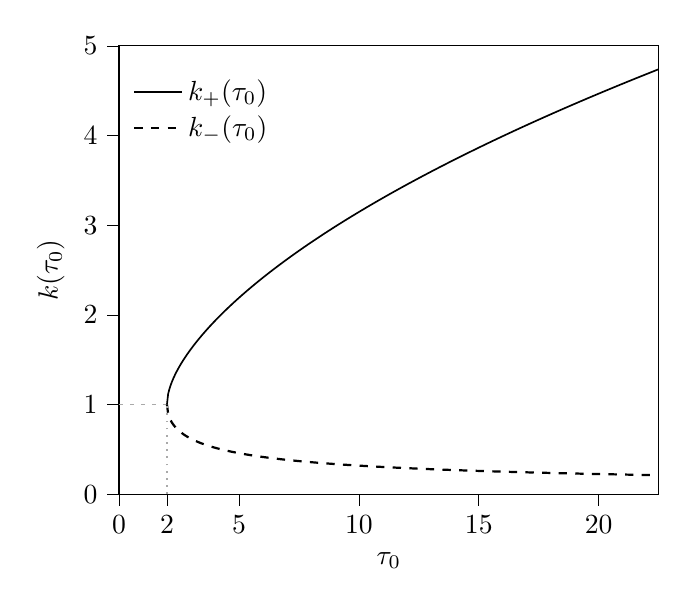
\begin{tikzpicture}

\definecolor{darkgray}{RGB}{169,169,169}
\definecolor{darkgray176}{RGB}{176,176,176}

\begin{axis}[
legend cell align={left},
legend style={
  fill opacity=0.8,
  draw opacity=1,
  text opacity=1,
  at={(0.01,0.95)},
  anchor=north west,
  draw=none
},
tick align=outside,
tick pos=left,
x grid style={darkgray176},
xlabel={\(\displaystyle \tau_0\)},
xmin=0, xmax=22.5,
xtick style={color=black},
y grid style={darkgray176},
ylabel={\(\displaystyle k(\tau_0)\)},
ymin=0, ymax=5,
ytick style={color=black},
xtick={0,2,5,10,15,20}, %afegit a ma
]
\path [draw=darkgray, semithick, dash pattern=on 1.5pt off 2.475pt]
(axis cs:0,1)
--(axis cs:2,1);

\addplot [semithick, black]
table {%
2 1
2.04902451225613 1.1168168000538
2.09804902451226 1.16874583266948
2.14707353676838 1.20996907879261
2.19609804902451 1.24563377354352
2.24512256128064 1.27773402875366
2.29414707353677 1.30729283131175
2.3431715857929 1.33491811026942
2.39219609804902 1.36100615291813
2.44122061030515 1.38583237958527
2.49024512256128 1.40959745757456
2.53926963481741 1.43245299190741
2.58829414707354 1.45451686745395
2.63731865932966 1.47588292272881
2.68634317158579 1.4966273225024
2.73536768384192 1.51681290987781
2.78439219609805 1.53649226973201
2.83341670835418 1.55570994132093
2.88244122061031 1.57450405222229
2.93146573286643 1.59290754851231
2.98049024512256 1.6109491368331
3.02951475737869 1.62865401678076
3.07853926963482 1.64604445799406
3.12756378189095 1.66314026040202
3.17658829414707 1.67995912531485
3.2256128064032 1.6965169576089
3.27463731865933 1.71282811403396
3.32366183091546 1.72890560894476
3.37268634317159 1.74476128605844
3.42171085542771 1.76040596285836
3.47073536768384 1.7758495527916
3.51975987993997 1.7911011693001
3.5687843921961 1.80616921488456
3.61780890445223 1.82106145775459
3.66683341670835 1.83578509811914
3.71585792896448 1.85034682578112
3.76488244122061 1.86475287039304
3.81390695347674 1.87900904548718
3.86293146573287 1.89312078719927
3.91195597798899 1.90709318844842
3.96098049024512 1.92093102920989
4.01000500250125 1.93463880341415
4.05902951475738 1.94822074292179
4.10805402701351 1.96168083895465
4.15707853926963 1.97502286130634
4.20610305152576 1.9882503756078
4.25512756378189 2.00136675888408
4.30415207603802 2.01437521360519
4.35317658829415 2.02727878040605
4.40220110055028 2.04008034962708
4.4512256128064 2.05278267180669
4.50025012506253 2.06538836724035
4.54927463731866 2.07789993470606
4.59829914957479 2.09031975944381
4.64732366183092 2.10265012046582
4.69634817408704 2.1148931972653
4.74537268634317 2.12705107598339
4.7943971985993 2.13912575508701
4.84342171085543 2.1511191506046
4.89244622311156 2.16303310096118
4.94147073536768 2.17486937144995
4.99049524762381 2.18662965837327
5.03951975987994 2.1983155928828
5.08854427213607 2.20992874454508
5.1375687843922 2.2214706246564
5.18659329664832 2.23294268932838
5.23561780890445 2.24434634236324
5.28464232116058 2.25568293793647
5.33366683341671 2.26695378310226
5.38269134567284 2.27816014013605
5.43171585792896 2.28930322872706
5.48074037018509 2.30038422803232
5.52976488244122 2.31140427860305
5.57878939469735 2.32236448419282
5.62781390695348 2.33326591345642
5.6768384192096 2.34410960154752
5.72586293146573 2.35489655162227
5.77488744372186 2.36562773625579
5.82391195597799 2.37630409877755
5.87293646823412 2.3869265545314
5.92196098049024 2.39749599206528
5.97098549274637 2.40801327425561
6.0200100050025 2.41847923937048
6.06903451725863 2.42889470207591
6.11805902951476 2.43926045438882
6.16708354177088 2.4495772665801
6.21610805402701 2.45984588803105
6.26513256628314 2.47006704804607
6.31415707853927 2.48024145662443
6.3631815907954 2.49036980519346
6.41220610305153 2.50045276730567
6.46123061530765 2.51049099930194
6.51025512756378 2.52048514094273
6.55927963981991 2.53043581600925
6.60830415207604 2.54034363287636
6.65732866433217 2.55020918505876
6.70635317658829 2.56003305173204
6.75537768884442 2.56981579822999
6.80440220110055 2.57955797651951
6.85342671335668 2.58926012565431
6.90245122561281 2.59892277220866
6.95147573786893 2.60854643069214
7.00050025012506 2.61813160394645
7.04952476238119 2.62767878352532
7.09854927463732 2.63718845005828
7.14757378689345 2.64666107359917
7.19659829914957 2.65609711396024
7.2456228114057 2.66549702103244
7.29464732366183 2.67486123509276
7.34367183591796 2.68419018709908
7.39269634817409 2.69348429897337
7.44172086043022 2.70274398387356
7.49074537268634 2.71196964645484
7.53976988494247 2.72116168312081
7.5887943971986 2.73032048226496
7.63781890945473 2.73944642450289
7.68684342171086 2.74853988289588
7.73586793396698 2.757601223166
7.78489244622311 2.76663080390324
7.83391695847924 2.77562897676507
7.88294147073537 2.78459608666872
7.9319659829915 2.79353247197648
7.98099049524762 2.80243846467435
8.03001500750375 2.81131439054445
8.07903951975988 2.82016056933119
8.12806403201601 2.82897731490179
8.17708854427214 2.83776493540115
8.22611305652826 2.84652373340145
8.27513756878439 2.8552540060466
8.32416208104052 2.86395604519186
8.37318659329665 2.87263013753877
8.42221110555278 2.88127656476555
8.4712356178089 2.88989560365325
8.52026013006503 2.89848752620777
8.56928464232116 2.90705259977786
8.61830915457729 2.91559108716938
8.66733366683342 2.92410324675588
8.71635817908954 2.93258933258568
8.76538269134567 2.94104959448555
8.8144072036018 2.94948427816118
8.86343171585793 2.95789362529454
8.91245622811406 2.96627787363819
8.96148074037018 2.97463725710679
9.01050525262631 2.98297200586572
9.05952976488244 2.99128234641717
9.10855427713857 2.99956850168352
9.1575787893947 3.00783069108833
9.20660330165083 3.01606913063491
9.25562781390695 3.02428403298259
9.30465232616308 3.03247560752082
9.35367683841921 3.040644060441
9.40270135067534 3.04878959480644
9.45172586293146 3.05691241062016
9.50075037518759 3.06501270489085
9.54977488744372 3.07309067169698
9.59879939969985 3.0811465022491
9.64782391195598 3.08918038495044
9.69684842421211 3.09719250545576
9.74587293646823 3.10518304672873
9.79489744872436 3.11315218909761
9.84392196098049 3.12110011030954
9.89294647323662 3.12902698558328
9.94197098549275 3.13693298766059
9.99099549774887 3.14481828685628
10.040020010005 3.15268305110689
10.0890445222611 3.16052744601809
10.1380690345173 3.16835163491091
10.1870935467734 3.17615577886673
10.2361180590295 3.18394003677112
10.2851425712856 3.19170456535655
10.3341670835418 3.19944951924407
10.3831915957979 3.20717505098388
10.432216108054 3.2148813110949
10.4812406203102 3.22256844810339
10.5302651325663 3.23023660858055
10.5792896448224 3.23788593717925
10.6283141570785 3.24551657666985
10.6773386693347 3.25312866797512
10.7263631815908 3.26072235020434
10.7753876938469 3.26829776068659
10.8244122061031 3.27585503500321
10.8734367183592 3.28339430701955
10.9224612306153 3.29091570891586
10.9714857428714 3.29841937121759
11.0205102551276 3.30590542282488
11.0695347673837 3.31337399104141
11.1185592796398 3.32082520160256
11.1675837918959 3.32825917870295
11.2166083041521 3.33567604502334
11.2656328164082 3.34307592175691
11.3146573286643 3.35045892863492
11.3636818409205 3.3578251839519
11.4127063531766 3.3651748045901
11.4617308654327 3.37250790604358
11.5107553776888 3.37982460244165
11.559779889945 3.38712500657181
11.6088044022011 3.39440922990226
11.6578289144572 3.4016773826038
11.7068534267134 3.40892957357135
11.7558779389695 3.41616591044498
11.8049024512256 3.4233864996305
11.8539269634817 3.43059144631954
11.9029514757379 3.43778085450933
11.951975987994 3.44495482702193
12.0010005002501 3.45211346552317
12.0500250125063 3.45925687054109
12.0990495247624 3.4663851414841
12.1480740370185 3.47349837665866
12.1970985492746 3.4805966732867
12.2461230615308 3.48768012752257
12.2951475737869 3.49474883446977
12.344172086043 3.50180288819721
12.3931965982991 3.50884238175527
12.4422211105553 3.51586740719142
12.4912456228114 3.52287805556561
12.5402701350675 3.52987441696531
12.5892946473237 3.53685658052027
12.6383191595798 3.54382463441699
12.6873436718359 3.55077866591289
12.736368184092 3.55771876135023
12.7853926963482 3.56464500616972
12.8344172086043 3.57155748492391
12.8834417208604 3.57845628129027
12.9324662331166 3.58534147808411
12.9814907453727 3.59221315727111
13.0305152576288 3.59907139997977
13.0795397698849 3.6059162865135
13.1285642821411 3.61274789636255
13.1775887943972 3.6195663082157
13.2266133066533 3.62637159997171
13.2756378189095 3.63316384875062
13.3246623311656 3.63994313090473
13.3736868434217 3.6467095220295
13.4227113556778 3.65346309697418
13.471735867934 3.66020392985223
13.5207603801901 3.66693209405163
13.5697848924462 3.67364766224492
13.6188094047024 3.68035070639908
13.6678339169585 3.6870412977853
13.7168584292146 3.69371950698847
13.7658829414707 3.70038540391655
13.8149074537269 3.70703905780982
13.863931965983 3.71368053724986
13.9129564782391 3.7203099101685
13.9619809904952 3.72692724385649
14.0110055027514 3.73353260497212
14.0600300150075 3.74012605954959
14.1090545272636 3.74670767300736
14.1580790395198 3.75327751015623
14.2071035517759 3.75983563520737
14.256128064032 3.76638211178018
14.3051525762881 3.77291700290999
14.3541770885443 3.7794403710557
14.4032016008004 3.78595227810721
14.4522261130565 3.79245278539277
14.5012506253127 3.79894195368622
14.5502751375688 3.80541984321408
14.5992996498249 3.81188651366252
14.648324162081 3.81834202418423
14.6973486743372 3.82478643340518
14.7463731865933 3.83121979943125
14.7953976988494 3.83764217985479
14.8444222111056 3.84405363176099
14.8934467233617 3.85045421173429
14.9424712356178 3.85684397586449
14.9914957478739 3.86322297975297
15.0405202601301 3.86959127851865
15.0895447723862 3.87594892680393
15.1385692846423 3.88229597878054
15.1875937968984 3.88863248815525
15.2366183091546 3.89495850817553
15.2856428214107 3.9012740916351
15.3346673336668 3.90757929087943
15.383691845923 3.91387415781108
15.4327163581791 3.92015874389504
15.4817408704352 3.92643310016392
15.5307653826913 3.93269727722313
15.5797898949475 3.93895132525587
15.6288144072036 3.9451952940282
15.6778389194597 3.95142923289386
15.7268634317159 3.95765319079916
15.775887943972 3.96386721628771
15.8249124562281 3.97007135750512
15.8739369684842 3.97626566220359
15.9229614807404 3.98245017774648
15.9719859929965 3.98862495111279
16.0210105052526 3.99479002890153
16.0700350175088 4.00094545733612
16.1190595297649 4.00709128226863
16.168084042021 4.01322754918401
16.2171085542771 4.01935430320424
16.2661330665333 4.02547158909245
16.3151575787894 4.03157945125691
16.3641820910455 4.03767793375503
16.4132066033017 4.04376708029729
16.4622311155578 4.04984693425107
16.5112556278139 4.05591753864449
16.56028014007 4.06197893617012
16.6093046523262 4.06803116918871
16.6583291645823 4.07407427973283
16.7073536768384 4.08010830951045
16.7563781890945 4.08613329990849
16.8054027013507 4.09214929199628
16.8544272136068 4.09815632652907
16.9034517258629 4.10415444395136
16.9524762381191 4.11014368440028
17.0015007503752 4.11612408770885
17.0505252626313 4.12209569340931
17.0995497748874 4.12805854073625
17.1485742871436 4.1340126686298
17.1975987993997 4.13995811573876
17.2466233116558 4.1458949204237
17.295647823912 4.15182312075994
17.3446723361681 4.15774275454056
17.3936968484242 4.16365385927942
17.4427213606803 4.16955647221396
17.4917458729365 4.17545063030817
17.5407703851926 4.18133637025538
17.5897948974487 4.18721372848107
17.6388194097049 4.19308274114561
17.687843921961 4.19894344414704
17.7368684342171 4.20479587312366
17.7858929464732 4.21064006345679
17.8349174587294 4.21647605027331
17.8839419709855 4.22230386844826
17.9329664832416 4.2281235526074
17.9819909954977 4.23393513712973
18.0310155077539 4.23973865614995
18.08004002001 4.24553414356091
18.1290645322661 4.25132163301605
18.1780890445223 4.25710115793177
18.2271135567784 4.26287275148978
18.2761380690345 4.26863644663945
18.3251625812906 4.27439227610007
18.3741870935468 4.28014027236314
18.4232116058029 4.28588046769461
18.472236118059 4.29161289413708
18.5212606303152 4.29733758351196
18.5702851425713 4.30305456742167
18.6193096548274 4.30876387725174
18.6683341670835 4.31446554417288
18.7173586793397 4.32015959914312
18.7663831915958 4.32584607290979
18.8154077038519 4.33152499601159
18.8644322161081 4.33719639878056
18.9134567283642 4.34286031134405
18.9624812406203 4.3485167636267
19.0115057528764 4.35416578535232
19.0605302651326 4.35980740604582
19.1095547773887 4.36544165503508
19.1585792896448 4.37106856145279
19.207603801901 4.3766881542383
19.2566283141571 4.38230046213941
19.3056528264132 4.38790551371418
19.3546773386693 4.39350333733269
19.4037018509255 4.39909396117875
19.4527263631816 4.40467741325167
19.5017508754377 4.41025372136795
19.5507753876938 4.41582291316295
19.59979989995 4.42138501609254
19.6488244122061 4.42694005743478
19.6978489244622 4.43248806429152
19.7468734367184 4.43802906359001
19.7958979489745 4.44356308208448
19.8449224612306 4.4490901463577
19.8939469734867 4.45461028282256
19.9429714857429 4.46012351772356
19.991995997999 4.46562987713834
20.0410205102551 4.47112938697918
20.0900450225113 4.47662207299448
20.1390695347674 4.4821079607702
20.1880940470235 4.48758707573131
20.2371185592796 4.49305944314325
20.2861430715358 4.49852508811328
20.3351675837919 4.50398403559193
20.384192096048 4.50943631037436
20.4332166083041 4.51488193710169
20.4822411205603 4.52032094026241
20.5312656328164 4.52575334419366
20.5802901450725 4.53117917308257
20.6293146573287 4.53659845096756
20.6783391695848 4.54201120173963
20.7273636818409 4.54741744914362
20.776388194097 4.55281721677948
20.8254127063532 4.55821052810353
20.8744372186093 4.56359740642964
20.9234617308654 4.56897787493052
20.9724862431216 4.57435195663887
21.0215107553777 4.57971967444857
21.0705352676338 4.58508105111592
21.1195597798899 4.59043610926071
21.1685842921461 4.59578487136746
21.2176088044022 4.60112735978649
21.2666333166583 4.60646359673511
21.3156578289145 4.61179360429869
21.3646823411706 4.61711740443177
21.4137068534267 4.62243501895916
21.4627313656828 4.62774646957703
21.511755877939 4.63305177785395
21.5607803901951 4.63835096523197
21.6098049024512 4.64364405302764
21.6588294147074 4.64893106243308
21.7078539269635 4.65421201451696
21.7568784392196 4.65948693022556
21.8059029514757 4.66475583038372
21.8549274637319 4.67001873569587
21.903951975988 4.67527566674698
21.9529764882441 4.68052664400357
22.0020010005003 4.68577168781461
22.0510255127564 4.69101081841255
22.1000500250125 4.69624405591416
22.1490745372686 4.70147142032156
22.1980990495248 4.70669293152307
22.2471235617809 4.71190860929416
22.296148074037 4.71711847329831
22.3451725862931 4.72232254308796
22.3941970985493 4.72752083810534
22.4432216108054 4.73271337768337
22.4922461230615 4.73790018104651
22.5412706353177 4.74308126731165
22.5902951475738 4.74825665548891
22.6393196598299 4.75342636448251
22.688344172086 4.75859041309158
22.7373686843422 4.76374882001102
22.7863931965983 4.76890160383226
22.8354177088544 4.77404878304409
22.8844422211106 4.77919037603349
22.9334667333667 4.78432640108635
22.9824912456228 4.78945687638831
23.0315157578789 4.79458182002551
23.0805402701351 4.79970124998535
23.1295647823912 4.80481518415728
23.1785892946473 4.80992364033349
23.2276138069035 4.81502663620972
23.2766383191596 4.82012418938594
23.3256628314157 4.82521631736714
23.3746873436718 4.83030303756399
23.423711855928 4.83538436729358
23.4727363681841 4.84046032378013
23.5217608804402 4.8455309241557
23.5707853926963 4.85059618546086
23.6198099049525 4.8556561246454
23.6688344172086 4.86071075856897
23.7178589294647 4.86576010400183
23.7668834417209 4.87080417762542
23.815907953977 4.8758429960331
23.8649324662331 4.88087657573077
23.9139569784892 4.88590493313753
23.9629814907454 4.89092808458629
24.0120060030015 4.89594604632446
24.0610305152576 4.90095883451453
24.1100550275138 4.90596646523472
24.1590795397699 4.9109689544796
24.208104052026 4.91596631816068
24.2571285642821 4.92095857210705
24.3061530765383 4.92594573206594
24.3551775887944 4.93092781370334
24.4042021010505 4.9359048326046
24.4532266133067 4.94087680427498
24.5022511255628 4.94584374414025
24.5512756378189 4.95080566754728
24.600300150075 4.95576258976456
24.6493246623312 4.96071452598281
24.6983491745873 4.9656614913155
24.7473736868434 4.97060350079943
24.7963981990995 4.97554056939527
24.8454227113557 4.98047271198808
24.8944472236118 4.98539994338788
24.9434717358679 4.99032227833017
24.9924962481241 4.99523973147643
25.0415207603802 5.00015231741469
25.0905452726363 5.00506005066001
25.1395697848924 5.00996294565501
25.1885942971486 5.01486101677038
25.2376188094047 5.01975427830537
25.2866433216608 5.02464274448829
25.335667833917 5.02952642947703
25.3846923461731 5.03440534735951
25.4337168584292 5.03927951215422
25.4827413706853 5.04414893781062
25.5317658829415 5.04901363820971
25.5807903951976 5.05387362716444
25.6298149074537 5.05872891842019
25.6788394197099 5.06357952565524
25.727863931966 5.06842546248125
25.7768884442221 5.07326674244369
25.8259129564782 5.07810337902228
25.8749374687344 5.08293538563149
25.9239619809905 5.08776277562093
25.9729864932466 5.09258556227581
26.0220110055028 5.0974037588174
26.0710355177589 5.10221737840342
26.120060030015 5.10702643412851
26.1690845422711 5.1118309390246
26.2181090545273 5.11663090606142
26.2671335667834 5.12142634814682
26.3161580790395 5.12621727812725
26.3651825912956 5.13100370878814
26.4142071035518 5.13578565285433
26.4632316158079 5.14056312299044
26.512256128064 5.14533613180131
26.5612806403202 5.15010469183237
26.6103051525763 5.15486881557004
26.6593296648324 5.15962851544211
26.7083541770885 5.16438380381815
26.7573786893447 5.16913469300988
26.8064032016008 5.17388119527155
26.8554277138569 5.1786233228003
26.9044522261131 5.18336108773658
26.9534767383692 5.18809450216446
27.0025012506253 5.19282357811205
27.0515257628814 5.19754832755184
27.1005502751376 5.20226876240105
27.1495747873937 5.20698489452202
27.1985992996498 5.21169673572253
27.247623811906 5.21640429775619
27.2966483241621 5.22110759232276
27.3456728364182 5.22580663106849
27.3946973486743 5.23050142558649
27.4437218609305 5.23519198741708
27.4927463731866 5.23987832804807
27.5417708854427 5.24456045891517
27.5907953976988 5.24923839140224
27.639819909955 5.25391213684172
27.6888444222111 5.25858170651484
27.7378689344672 5.26324711165206
27.7868934467234 5.26790836343331
27.8359179589795 5.27256547298833
27.8849424712356 5.277218451397
27.9339669834917 5.28186730968966
27.9829914957479 5.28651205884739
28.032016008004 5.29115270980235
28.0810405202601 5.29578927343804
28.1300650325163 5.30042176058968
28.1790895447724 5.30505018204444
28.2281140570285 5.30967454854177
28.2771385692846 5.31429487077369
28.3261630815408 5.3189111593851
28.3751875937969 5.32352342497405
28.424212106053 5.32813167809203
28.4732366183092 5.33273592924428
28.5222611305653 5.33733618889004
28.5712856428214 5.34193246744288
28.6203101550775 5.34652477527092
28.6693346673337 5.35111312269717
28.7183591795898 5.35569751999976
28.7673836918459 5.36027797741223
28.816408204102 5.36485450512382
28.8654327163582 5.36942711327969
28.9144572286143 5.37399581198124
28.9634817408704 5.37856061128636
29.0125062531266 5.38312152120967
29.0615307653827 5.38767855172281
29.1105552776388 5.39223171275468
29.1595797898949 5.39678101419171
29.2086043021511 5.40132646587811
29.2576288144072 5.40586807761611
29.3066533266633 5.41040585916624
29.3556778389195 5.41493982024756
29.4047023511756 5.41946997053791
29.4537268634317 5.42399631967414
29.5027513756878 5.42851887725239
29.551775887944 5.4330376528283
29.6008004002001 5.43755265591727
29.6498249124562 5.44206389599467
29.6988494247124 5.44657138249613
29.7478739369685 5.4510751248177
29.7968984492246 5.45557513231614
29.8459229614807 5.46007141430913
29.8949474737369 5.46456398007552
29.943971985993 5.4690528388555
29.9929964982491 5.47353799985089
30.0420210105053 5.47801947222535
30.0910455227614 5.48249726510456
30.1400700350175 5.4869713875765
30.1890945472736 5.49144184869163
30.2381190595298 5.4959086574631
30.2871435717859 5.50037182286701
30.336168084042 5.50483135384259
30.3851925962981 5.50928725929241
30.4342171085543 5.5137395480826
30.4832416208104 5.51818822904309
30.5322661330665 5.52263331096774
30.5812906453227 5.52707480261464
30.6303151575788 5.53151271270623
30.6793396698349 5.53594704992957
30.728364182091 5.54037782293651
30.7773886943472 5.54480504034387
30.8264132066033 5.5492287107337
30.8754377188594 5.55364884265341
30.9244622311156 5.558065444616
30.9734867433717 5.56247852510027
31.0225112556278 5.56688809255098
31.0715357678839 5.57129415537905
31.1205602801401 5.57569672196176
31.1695847923962 5.58009580064293
31.2186093046523 5.58449139973313
31.2676338169085 5.58888352750982
31.3166583291646 5.59327219221759
31.3656828414207 5.5976574020683
31.4147073536768 5.60203916524127
31.463731865933 5.60641748988349
31.5127563781891 5.61079238410976
31.5617808904452 5.61516385600291
31.6108054027013 5.61953191361392
31.6598299149575 5.62389656496216
31.7088544272136 5.62825781803553
31.7578789394697 5.63261568079061
31.8069034517259 5.63697016115289
31.855927963982 5.6413212670169
31.9049524762381 5.64566900624639
31.9539769884942 5.65001338667449
32.0030015007504 5.6543544161039
32.0520260130065 5.65869210230702
32.1010505252626 5.66302645302616
32.1500750375188 5.66735747597367
32.1990995497749 5.6716851788321
32.248124062031 5.6760095692544
32.2971485742871 5.68033065486403
32.3461730865433 5.68464844325515
32.3951975987994 5.68896294199277
32.4442221110555 5.69327415861292
32.4932466233117 5.69758210062279
32.5422711355678 5.70188677550087
32.5912956478239 5.70618819069715
32.64032016008 5.71048635363322
32.6893446723362 5.71478127170247
32.7383691845923 5.71907295227021
32.7873936968484 5.72336140267381
32.8364182091046 5.72764663022288
32.8854427213607 5.73192864219942
32.9344672336168 5.73620744585791
32.9834917458729 5.74048304842553
33.0325162581291 5.74475545710225
33.0815407703852 5.74902467906101
33.1305652826413 5.75329072144782
33.1795897948975 5.75755359138194
33.2286143071536 5.76181329595603
33.2776388194097 5.76606984223623
33.3266633316658 5.77032323726235
33.375687843922 5.77457348804801
33.4247123561781 5.77882060158073
33.4737368684342 5.78306458482213
33.5227613806903 5.787305444708
33.5717858929465 5.7915431881485
33.6208104052026 5.79577782202822
33.6698349174587 5.80000935320637
33.7188594297149 5.80423778851691
33.767883941971 5.80846313476864
33.8169084542271 5.81268539874536
33.8659329664832 5.81690458720598
33.9149574787394 5.82112070688468
33.9639819909955 5.82533376449101
34.0130065032516 5.82954376671001
34.0620310155078 5.83375072020238
34.1110555277639 5.83795463160452
34.16008004002 5.84215550752877
34.2091045522761 5.84635335456342
34.2581290645323 5.85054817927291
34.3071535767884 5.85473998819791
34.3561780890445 5.85892878785546
34.4052026013007 5.86311458473908
34.4542271135568 5.8672973853189
34.5032516258129 5.87147719604176
34.552276138069 5.87565402333135
34.6013006503252 5.87982787358831
34.6503251625813 5.88399875319036
34.6993496748374 5.88816666849238
34.7483741870935 5.89233162582658
34.7973986993497 5.89649363150257
34.8464232116058 5.90065269180749
34.8954477238619 5.90480881300612
34.9444722361181 5.908962001341
34.9934967483742 5.91311226303251
35.0425212606303 5.91725960427903
35.0915457728864 5.92140403125701
35.1405702851426 5.92554555012107
35.1895947973987 5.92968416700416
35.2386193096548 5.93381988801762
35.287643821911 5.93795271925131
35.3366683341671 5.94208266677369
35.3856928464232 5.94620973663197
35.4347173586793 5.95033393485217
35.4837418709355 5.95445526743923
35.5327663831916 5.95857374037717
35.5817908954477 5.9626893596291
35.6308154077038 5.9668021311374
35.67983991996 5.97091206082377
35.7288644322161 5.97501915458938
35.7778889444722 5.97912341831491
35.8269134567284 5.9832248578607
35.8759379689845 5.98732347906683
35.9249624812406 5.99141928775322
35.9739869934967 5.99551228971972
36.0230115057529 5.9996024907462
36.072036018009 6.0036898965927
36.1210605302651 6.00777451299944
36.1700850425213 6.01185634568699
36.2191095547774 6.01593540035633
36.2681340670335 6.02001168268894
36.3171585792896 6.02408519834691
36.3661830915458 6.02815595297301
36.4152076038019 6.03222395219083
36.464232116058 6.03628920160482
36.5132566283142 6.04035170680038
36.5622811405703 6.04441147334402
36.6113056528264 6.04846850678335
36.6603301650825 6.05252281264727
36.7093546773387 6.05657439644596
36.7583791895948 6.06062326367105
36.8074037018509 6.06466941979568
36.8564282141071 6.06871287027456
36.9054527263632 6.0727536205441
36.9544772386193 6.07679167602245
37.0035017508754 6.08082704210966
37.0525262631316 6.08485972418766
37.1015507753877 6.08888972762045
37.1505752876438 6.0929170577541
37.1995997998999 6.0969417199169
37.2486243121561 6.10096371941939
37.2976488244122 6.10498306155448
37.3466733366683 6.10899975159751
37.3956978489245 6.11301379480635
37.4447223611806 6.11702519642145
37.4937468734367 6.12103396166597
37.5427713856928 6.1250400957458
37.591795897949 6.12904360384971
37.6408204102051 6.13304449114936
37.6898449224612 6.13704276279941
37.7388694347174 6.14103842393762
37.7878939469735 6.14503147968489
37.8369184592296 6.14902193514536
37.8859429714857 6.15300979540647
37.9349674837419 6.15699506553906
37.983991995998 6.16097775059743
38.0330165082541 6.1649578556194
38.0820410205103 6.16893538562644
38.1310655327664 6.17291034562368
38.1800900450225 6.17688274060001
38.2291145572786 6.18085257552818
38.2781390695348 6.18481985536484
38.3271635817909 6.18878458505061
38.376188094047 6.19274676951018
38.4252126063031 6.19670641365235
38.4742371185593 6.20066352237016
38.5232616308154 6.20461810054087
38.5722861430715 6.20857015302611
38.6213106553277 6.21251968467192
38.6703351675838 6.21646670030881
38.7193596798399 6.22041120475186
38.7683841920961 6.22435320280076
38.8174087043522 6.22829269923989
38.8664332166083 6.23222969883839
38.9154577288644 6.23616420635023
38.9644822411206 6.24009622651426
39.0135067533767 6.2440257640543
39.0625312656328 6.24795282367922
39.1115557778889 6.25187741008294
39.1605802901451 6.25579952794457
39.2096048024012 6.25971918192846
39.2586293146573 6.26363637668421
39.3076538269135 6.26755111684681
39.3566783391696 6.27146340703667
39.4057028514257 6.27537325185967
39.4547273636818 6.27928065590725
39.503751875938 6.28318562375646
39.5527763881941 6.28708815997004
39.6018009004502 6.29098826909644
39.6508254127064 6.29488595566994
39.6998499249625 6.29878122421067
39.7488744372186 6.30267407922469
39.7978989494747 6.30656452520404
39.8469234617309 6.31045256662683
39.895947973987 6.31433820795726
39.9449724862431 6.31822145364569
39.9939969984992 6.32210230812874
40.0430215107554 6.3259807758293
40.0920460230115 6.32985686115659
40.1410705352676 6.33373056850629
40.1900950475238 6.33760190226049
40.2391195597799 6.34147086678784
40.288144072036 6.34533746644356
40.3371685842921 6.34920170556952
40.3861930965483 6.35306358849427
40.4352176088044 6.35692311953313
40.4842421210605 6.36078030298824
40.5332666333167 6.36463514314858
40.5822911455728 6.36848764429008
40.6313156578289 6.37233781067564
40.680340170085 6.37618564655521
40.7293646823412 6.3800311561658
40.7783891945973 6.38387434373159
40.8274137068534 6.38771521346397
40.8764382191096 6.39155376956157
40.9254627313657 6.39539001621032
40.9744872436218 6.39922395758353
41.0235117558779 6.40305559784192
41.0725362681341 6.40688494113369
41.1215607803902 6.41071199159454
41.1705852926463 6.41453675334777
41.2196098049024 6.41835923050429
41.2686343171586 6.4221794271627
41.3176588294147 6.42599734740933
41.3666833416708 6.42981299531829
41.415707853927 6.43362637495152
41.4647323661831 6.43743749035885
41.5137568784392 6.44124634557804
41.5627813906953 6.44505294463486
41.6118059029515 6.44885729154308
41.6608304152076 6.45265939030458
41.7098549274637 6.45645924490936
41.7588794397199 6.46025685933562
41.807903951976 6.46405223754979
41.8569284642321 6.46784538350657
41.9059529764882 6.47163630114901
41.9549774887444 6.47542499440853
42.0040020010005 6.47921146720497
42.0530265132566 6.48299572344665
42.1020510255128 6.48677776703043
42.1510755377689 6.49055760184171
42.200100050025 6.49433523175452
42.2491245622811 6.49811066063157
42.2981490745373 6.50188389232425
42.3471735867934 6.50565493067273
42.3961980990495 6.50942377950597
42.4452226113057 6.51319044264178
42.4942471235618 6.51695492388687
42.5432716358179 6.52071722703688
42.592296148074 6.52447735587643
42.6413206603302 6.52823531417919
42.6903451725863 6.53199110570788
42.7393696848424 6.53574473421435
42.7883941970985 6.5394962034396
42.8374187093547 6.54324551711386
42.8864432216108 6.54699267895659
42.9354677338669 6.55073769267653
42.9844922461231 6.55448056197179
43.0335167583792 6.55822129052983
43.0825412706353 6.56195988202754
43.1315657828914 6.56569634013129
43.1805902951476 6.56943066849693
43.2296148074037 6.57316287076987
43.2786393196598 6.57689295058511
43.327663831916 6.5806209115673
43.3766883441721 6.58434675733073
43.4257128564282 6.58807049147942
43.4747373686843 6.59179211760715
43.5237618809405 6.5955116392975
43.5727863931966 6.59922906012388
43.6218109054527 6.60294438364956
43.6708354177089 6.60665761342777
43.719859929965 6.61036875300165
43.7688844422211 6.61407780590438
43.8179089544772 6.61778477565914
43.8669334667334 6.62148966577921
43.9159579789895 6.62519247976799
43.9649824912456 6.628893221119
44.0140070035018 6.632591893316
44.0630315157579 6.63628849983295
44.112056028014 6.63998304413408
44.1610805402701 6.64367552967394
44.2101050525263 6.64736595989743
44.2591295647824 6.65105433823983
44.3081540770385 6.65474066812682
44.3571785892946 6.65842495297458
44.4062031015508 6.66210719618975
44.4552276138069 6.66578740116953
44.504252126063 6.66946557130167
44.5532766383192 6.67314170996453
44.6023011505753 6.67681582052714
44.6513256628314 6.68048790634916
44.7003501750875 6.68415797078102
44.7493746873437 6.68782601716386
44.7983991995998 6.69149204882963
44.8474237118559 6.6951560691011
44.8964482241121 6.69881808129189
44.9454727363682 6.70247808870653
44.9944972486243 6.70613609464045
45.0435217608804 6.70979210238008
45.0925462731366 6.71344611520283
45.1415707853927 6.71709813637713
45.1905952976488 6.72074816916251
45.239619809905 6.72439621680957
45.2886443221611 6.72804228256006
45.3376688344172 6.73168636964691
45.3866933466733 6.73532848129423
45.4357178589295 6.73896862071738
45.4847423711856 6.742606791123
45.5337668834417 6.74624299570901
45.5827913956978 6.74987723766468
45.631815907954 6.75350952017066
45.6808404202101 6.75713984639897
45.7298649324662 6.76076821951311
45.7788894447224 6.764394642668
45.8279139569785 6.76801911901009
45.8769384692346 6.77164165167735
45.9259629814907 6.77526224379932
45.9749874937469 6.77888089849712
46.024012006003 6.78249761888353
46.0730365182591 6.78611240806294
46.1220610305153 6.78972526913148
46.1710855427714 6.79333620517695
46.2201100550275 6.79694521927895
46.2691345672836 6.80055231450882
46.3181590795398 6.80415749392976
46.3671835917959 6.80776076059676
46.416208104052 6.81136211755673
46.4652326163081 6.81496156784845
46.5142571285643 6.81855911450267
46.5632816408204 6.82215476054207
46.6123061530765 6.82574850898135
46.6613306653327 6.82934036282722
46.7103551775888 6.83293032507845
46.7593796898449 6.83651839872589
46.8084042021011 6.8401045867525
46.8574287143572 6.84368889213339
46.9064532266133 6.84727131783584
46.9554777388694 6.85085186681933
47.0045022511256 6.85443054203554
47.0535267633817 6.85800734642846
47.1025512756378 6.86158228293432
47.1515757878939 6.86515535448168
47.2006003001501 6.86872656399144
47.2496248124062 6.87229591437688
47.2986493246623 6.87586340854367
47.3476738369185 6.8794290493899
47.3966983491746 6.88299283980611
47.4457228614307 6.88655478267535
47.4947473736868 6.89011488087313
47.543771885943 6.89367313726755
47.5927963981991 6.89722955471923
47.6418209104552 6.90078413608139
47.6908454227114 6.90433688419989
47.7398699349675 6.90788780191319
47.7888944472236 6.91143689205247
47.8379189594797 6.91498415744156
47.8869434717359 6.91852960089705
47.935967983992 6.92207322522825
47.9849924962481 6.92561503323727
48.0340170085043 6.929155027719
48.0830415207604 6.93269321146118
48.1320660330165 6.93622958724437
48.1810905452726 6.93976415784204
48.2301150575288 6.94329692602055
48.2791395697849 6.9468278945392
48.328164082041 6.95035706615023
48.3771885942971 6.95388444359887
48.4262131065533 6.95741002962335
48.4752376188094 6.96093382695494
48.5242621310655 6.96445583831794
48.5732866433217 6.96797606642977
48.6223111555778 6.97149451400092
48.6713356678339 6.97501118373503
48.72036018009 6.97852607832887
48.7693846923462 6.98203920047242
48.8184092046023 6.98555055284883
48.8674337168584 6.98906013813449
48.9164582291146 6.99256795899905
48.9654827413707 6.99607401810541
49.0145072536268 6.9995783181098
49.0635317658829 7.00308086166173
49.1125562781391 7.00658165140409
49.1615807903952 7.01008068997313
49.2106053026513 7.01357797999847
49.2596298149075 7.01707352410317
49.3086543271636 7.02056732490372
49.3576788394197 7.02405938501006
49.4067033516758 7.02754970702562
49.455727863932 7.03103829354736
49.5047523761881 7.03452514716572
49.5537768884442 7.03801027046474
49.6028014007004 7.041493666022
49.6518259129565 7.0449753364087
49.7008504252126 7.04845528418964
49.7498749374687 7.05193351192327
49.7988994497249 7.05541002216171
49.847923961981 7.05888481745076
49.8969484742371 7.0623579003299
49.9459729864932 7.06582927333239
49.9949974987494 7.06929893898521
50.0440220110055 7.0727668998091
50.0930465232616 7.07623315831862
50.1420710355178 7.07969771702213
50.1910955477739 7.08316057842183
50.24012006003 7.08662174501378
50.2891445722861 7.09008121928792
50.3381690845423 7.09353900372807
50.3871935967984 7.09699510081201
50.4362181090545 7.10044951301141
50.4852426213107 7.10390224279195
50.5342671335668 7.10735329261327
50.5832916458229 7.11080266492901
50.632316158079 7.11425036218684
50.6813406703352 7.11769638682847
50.7303651825913 7.12114074128969
50.7793896948474 7.12458342800035
50.8284142071035 7.12802444938443
50.8774387193597 7.13146380786001
50.9264632316158 7.13490150583934
50.9754877438719 7.13833754572881
51.0245122561281 7.14177192992901
51.0735367683842 7.14520466083474
51.1225612806403 7.14863574083501
51.1715857928964 7.15206517231307
51.2206103051526 7.15549295764644
51.2696348174087 7.15891909920694
51.3186593296648 7.16234359936066
51.367683841921 7.16576646046802
51.4167083541771 7.16918768488379
51.4657328664332 7.1726072749571
51.5147573786893 7.17602523303144
51.5637818909455 7.17944156144471
51.6128064032016 7.18285626252922
51.6618309154577 7.18626933861171
51.7108554277139 7.18968079201339
51.75987993997 7.19309062504992
51.8089044522261 7.19649884003146
51.8579289644822 7.19990543926268
51.9069534767384 7.20331042504276
51.9559779889945 7.20671379966545
52.0050025012506 7.21011556541904
52.0540270135068 7.21351572458642
52.1030515257629 7.21691427944505
52.152076038019 7.22031123226704
52.2011005502751 7.22370658531911
52.2501250625313 7.22710034086264
52.2991495747874 7.23049250115368
52.3481740870435 7.23388306844297
52.3971985992996 7.23727204497595
52.4462231115558 7.24065943299278
52.4952476238119 7.24404523472837
52.544272136068 7.24742945241238
52.5932966483242 7.25081208826924
52.6423211605803 7.25419314451817
52.6913456728364 7.25757262337321
52.7403701850925 7.26095052704322
52.7893946973487 7.26432685773191
52.8384192096048 7.26770161763782
52.8874437218609 7.2710748089544
52.9364682341171 7.27444643386997
52.9854927463732 7.27781649456778
53.0345172586293 7.28118499322599
53.0835417708854 7.28455193201771
53.1325662831416 7.287917313111
53.1815907953977 7.29128113866889
53.2306153076538 7.29464341084944
53.27963981991 7.29800413180566
53.3286643321661 7.30136330368564
53.3776888444222 7.30472092863247
53.4267133566783 7.30807700878431
53.4757378689345 7.3114315462744
53.5247623811906 7.31478454323106
53.5737868934467 7.31813600177771
53.6228114057028 7.32148592403289
53.671835917959 7.32483431211029
53.7208604302151 7.32818116811873
53.7698849424712 7.33152649416221
53.8189094547274 7.33487029233992
53.8679339669835 7.33821256474622
53.9169584792396 7.34155331347071
53.9659829914957 7.3448925405982
54.0150075037519 7.34823024820876
54.064032016008 7.35156643837771
54.1130565282641 7.35490111317564
54.1620810405203 7.35823427466843
54.2111055527764 7.36156592491726
54.2601300650325 7.36489606597866
54.3091545772886 7.36822469990445
54.3581790895448 7.37155182874181
54.4072036018009 7.37487745453332
54.456228114057 7.37820157931688
54.5052526263132 7.38152420512584
54.5542771385693 7.3848453339889
54.6033016508254 7.38816496793023
54.6523261630815 7.39148310896942
54.7013506753377 7.3947997591215
54.7503751875938 7.39811492039697
54.7993996998499 7.40142859480182
54.8484242121061 7.40474078433753
54.8974487243622 7.40805149100107
54.9464732366183 7.41136071678496
54.9954977488744 7.41466846367724
55.0445222611306 7.4179747336615
55.0935467733867 7.42127952871689
55.1425712856428 7.42458285081815
55.1915957978989 7.42788470193561
55.2406203101551 7.43118508403519
55.2896448224112 7.43448399907845
55.3386693346673 7.43778144902256
55.3876938469235 7.44107743582037
55.4367183591796 7.44437196142035
55.4857428714357 7.44766502776668
55.5347673836918 7.45095663679919
55.583791895948 7.45424679045345
55.6328164082041 7.45753549066072
55.6818409204602 7.46082273934798
55.7308654327164 7.46410853843797
55.7798899449725 7.46739288984917
55.8289144572286 7.47067579549584
55.8779389694847 7.47395725728801
55.9269634817409 7.4772372771315
55.975987993997 7.48051585692794
56.0250125062531 7.48379299857477
56.0740370185093 7.48706870396529
56.1230615307654 7.4903429749886
56.1720860430215 7.49361581352971
56.2211105552776 7.49688722146944
56.2701350675338 7.50015720068455
56.3191595797899 7.50342575304765
56.368184092046 7.50669288042728
56.4172086043021 7.50995858468791
56.4662331165583 7.51322286768992
56.5152576288144 7.51648573128963
56.5642821410705 7.51974717733936
56.6133066533267 7.52300720768735
56.6623311655828 7.52626582417786
56.7113556778389 7.52952302865111
56.760380190095 7.53277882294336
56.8094047023512 7.53603320888687
56.8584292146073 7.53928618830993
56.9074537268634 7.54253776303687
56.9564782391196 7.5457879348881
57.0055027513757 7.54903670568007
57.0545272636318 7.55228407722531
57.1035517758879 7.55553005133246
57.1525762881441 7.55877462980624
57.2016008004002 7.5620178144475
57.2506253126563 7.56525960705321
57.2996498249125 7.56850000941647
57.3486743371686 7.57173902332655
57.3976988494247 7.57497665056885
57.4467233616808 7.57821289292497
57.495747873937 7.58144775217268
57.5447723861931 7.58468123008595
57.5937968984492 7.58791332843496
57.6428214107054 7.59114404898609
57.6918459229615 7.59437339350196
57.7408704352176 7.59760136374145
57.7898949474737 7.60082796145966
57.8389194597299 7.60405318840797
57.887943971986 7.60727704633404
57.9369684842421 7.61049953698179
57.9859929964982 7.61372066209146
58.0350175087544 7.61694042339959
58.0840420210105 7.62015882263905
58.1330665332666 7.623375861539
58.1820910455228 7.62659154182499
58.2311155577789 7.62980586521889
58.280140070035 7.63301883343894
58.3291645822911 7.63623044819975
58.3781890945473 7.63944071121232
58.4272136068034 7.64264962418403
58.4762381190595 7.64585718881869
58.5252626313157 7.64906340681649
58.5742871435718 7.65226827987408
58.6233116558279 7.65547180968452
58.672336168084 7.65867399793733
58.7213606803402 7.66187484631849
58.7703851925963 7.66507435651044
58.8194097048524 7.66827253019209
58.8684342171086 7.67146936903886
58.9174587293647 7.67466487472265
58.9664832416208 7.67785904891188
59.0155077538769 7.68105189327148
59.0645322661331 7.68424340946292
59.1135567783892 7.6874335991442
59.1625812906453 7.69062246396986
59.2116058029014 7.69381000559103
59.2606303151576 7.69699622565539
59.3096548274137 7.70018112580718
59.3586793396698 7.70336470768727
59.407703851926 7.70654697293311
59.4567283641821 7.70972792317874
59.5057528764382 7.71290756005486
59.5547773886943 7.71608588518875
59.6038019009505 7.71926290020438
59.6528264132066 7.72243860672233
59.7018509254627 7.72561300635985
59.7508754377189 7.72878610073086
59.799899949975 7.73195789144595
59.8489244622311 7.73512838011242
59.8979489744872 7.73829756833423
59.9469734867434 7.74146545771208
59.9959979989995 7.74463204984336
60.0450225112556 7.74779734632219
60.0940470235118 7.75096134873944
60.1430715357679 7.75412405868271
60.192096048024 7.75728547773635
60.2411205602801 7.76044560748148
60.2901450725363 7.76360444949599
60.3391695847924 7.76676200535455
60.3881940970485 7.76991827662862
60.4372186093047 7.77307326488645
60.4862431215608 7.77622697169312
60.5352676338169 7.77937939861051
60.584292146073 7.78253054719732
60.6333166583292 7.78568041900911
60.6823411705853 7.78882901559825
60.7313656828414 7.79197633851401
60.7803901950975 7.79512238930247
60.8294147073537 7.79826716950663
60.8784392196098 7.80141068066633
60.9274637318659 7.80455292431832
60.9764882441221 7.80769390199624
61.0255127563782 7.81083361523065
61.0745372686343 7.813972065549
61.1235617808904 7.81710925447569
61.1725862931466 7.82024518353204
61.2216108054027 7.8233798542363
61.2706353176588 7.8265132681037
61.319659829915 7.8296454266464
61.3686843421711 7.83277633137354
61.4177088544272 7.83590598379124
61.4667333666833 7.83903438540258
61.5157578789395 7.84216153770766
61.5647823911956 7.84528744220357
61.6138069034517 7.84841210038441
61.6628314157078 7.8515355137413
61.711855927964 7.85465768376237
61.7608804402201 7.8577786119328
61.8099049524762 7.86089829973483
61.8589294647324 7.8640167486477
61.9079539769885 7.86713396014776
61.9569784892446 7.8702499357084
62.0060030015008 7.87336467680009
62.0550275137569 7.87647818489039
62.104052026013 7.87959046144394
62.1530765382691 7.8827015079225
62.2021010505253 7.8858113257849
62.2511255627814 7.88891991648713
62.3001500750375 7.89202728148228
62.3491745872936 7.89513342222057
62.3981990995498 7.89823834014937
62.4472236118059 7.90134203671319
62.496248124062 7.90444451335369
62.5452726363182 7.90754577150971
62.5942971485743 7.91064581261725
62.6433216608304 7.91374463810948
62.6923461730865 7.91684224941678
62.7413706853427 7.91993864796671
62.7903951975988 7.92303383518403
62.8394197098549 7.9261278124907
62.8884442221111 7.92922058130593
62.9374687343672 7.93231214304613
62.9864932466233 7.93540249912494
63.0355177588794 7.93849165095325
63.0845422711356 7.9415795999392
63.1335667833917 7.94466634748817
63.1825912956478 7.94775189500283
63.2316158079039 7.95083624388309
63.2806403201601 7.95391939552615
63.3296648324162 7.9570013513265
63.3786893446723 7.96008211267592
63.4277138569285 7.96316168096348
63.4767383691846 7.96624005757558
63.5257628814407 7.9693172438959
63.5747873936968 7.97239324130548
63.623811905953 7.97546805118265
63.6728364182091 7.97854167490311
63.7218609304652 7.98161411383989
63.7708854427214 7.98468536936336
63.8199099549775 7.98775544284126
63.8689344672336 7.9908243356387
63.9179589794897 7.99389204911814
63.9669834917459 7.99695858463945
64.016008004002 8.00002394355986
64.0650325162581 8.00308812723401
64.1140570285143 8.00615113701392
64.1630815407704 8.00921297424904
64.2121060530265 8.01227364028622
64.2611305652826 8.01533313646974
64.3101550775388 8.0183914641413
64.3591795897949 8.02144862464003
64.408204102051 8.02450461930252
64.4572286143072 8.02755944946279
64.5062531265633 8.03061311645233
64.5552776388194 8.03366562160009
64.6043021510755 8.03671696623247
64.6533266633317 8.03976715167337
64.7023511755878 8.04281617924415
64.7513756878439 8.04586405026369
64.8004002001001 8.04891076604834
64.8494247123562 8.05195632791196
64.8984492246123 8.05500073716592
64.9474737368684 8.05804399511909
64.9964982491246 8.0610861030779
65.0455227613807 8.06412706234627
65.0945472736368 8.06716687422568
65.1435717858929 8.07020554001514
65.1925962981491 8.07324306101122
65.2416208104052 8.07627943850802
65.2906453226613 8.07931467379722
65.3396698349175 8.08234876816807
65.3886943471736 8.0853817229074
65.4377188594297 8.0884135392996
65.4867433716858 8.09144421862666
65.535767883942 8.09447376216816
65.5847923961981 8.09750217120128
65.6338169084542 8.10052944700081
65.6828414207104 8.10355559083914
65.7318659329665 8.10658060398629
65.7808904452226 8.10960448770991
65.8299149574787 8.11262724327527
65.8789394697349 8.11564887194527
65.927963981991 8.11866937498047
65.9769884942471 8.12168875363908
66.0260130065032 8.12470700917695
66.0750375187594 8.1277241428476
66.1240620310155 8.13074015590222
66.1730865432716 8.13375504958967
66.2221110555278 8.1367688251565
66.2711355677839 8.13978148384692
66.32016008004 8.14279302690287
66.3691845922962 8.14580345556396
66.4182091045523 8.14881277106751
66.4672336168084 8.15182097464856
66.5162581290645 8.15482806753984
66.5652826413207 8.15783405097184
66.6143071535768 8.16083892617274
66.6633316658329 8.16384269436848
66.712356178089 8.16684535678273
66.7613806903452 8.16984691463691
66.8104052026013 8.17284736915018
66.8594297148574 8.17584672153946
66.9084542271136 8.17884497301944
66.9574787393697 8.18184212480258
67.0065032516258 8.1848381780991
67.0555277638819 8.18783313411702
67.1045522761381 8.19082699406212
67.1535767883942 8.193819759138
67.2026013006503 8.19681143054603
67.2516258129065 8.1998020094854
67.3006503251626 8.2027914971531
67.3496748374187 8.20577989474394
67.3986993496748 8.20876720345055
67.447723861931 8.21175342446337
67.4967483741871 8.2147385589707
67.5457728864432 8.21772260815864
67.5947973986993 8.22070557321116
67.6438219109555 8.22368745531006
67.6928464232116 8.226668255635
67.7418709354677 8.22964797536351
67.7908954477239 8.23262661567095
67.83991995998 8.23560417773058
67.8889444722361 8.23858066271353
67.9379689844922 8.2415560717888
67.9869934967484 8.24453040612327
68.0360180090045 8.24750366688172
68.0850425212606 8.25047585522684
68.1340670335168 8.25344697231919
68.1830915457729 8.25641701931726
68.232116058029 8.25938599737744
68.2811405702851 8.26235390765405
68.3301650825413 8.26532075129931
68.3791895947974 8.26828652946339
68.4282141070535 8.27125124329438
68.4772386193097 8.27421489393831
68.5262631315658 8.27717748253916
68.5752876438219 8.28013901023884
68.624312156078 8.28309947817725
68.6733366683342 8.2860588874922
68.7223611805903 8.2890172393195
68.7713856928464 8.29197453479291
68.8204102051025 8.29493077504418
68.8694347173587 8.29788596120302
68.9184592296148 8.30084009439713
68.9674837418709 8.30379317575222
69.0165082541271 8.30674520639197
69.0655327663832 8.30969618743806
69.1145572786393 8.31264612001018
69.1635817908954 8.31559500522603
69.2126063031516 8.31854284420132
69.2616308154077 8.32148963804979
69.3106553276638 8.32443538788319
69.35967983992 8.3273800948113
69.4087043521761 8.33032375994194
69.4577288644322 8.33326638438097
69.5067533766883 8.33620796923228
69.5557778889445 8.33914851559783
69.6048024012006 8.34208802457761
69.6538269134567 8.34502649726968
69.7028514257129 8.34796393477017
69.751875937969 8.35090033817326
69.8009004502251 8.35383570857121
69.8499249624812 8.35677004705436
69.8989494747374 8.35970335471112
69.9479739869935 8.36263563262802
69.9969984992496 8.36556688188963
70.0460230115058 8.36849710357867
70.0950475237619 8.3714262987759
70.144072036018 8.37435446856025
70.1930965482741 8.37728161400871
70.2421210605303 8.3802077361964
70.2911455727864 8.38313283619657
70.3401700850425 8.38605691508059
70.3891945972986 8.38897997391794
70.4382191095548 8.39190201377626
70.4872436218109 8.39482303572131
70.536268134067 8.39774304081699
70.5852926463232 8.40066203012536
70.6343171585793 8.40358000470662
70.6833416708354 8.40649696561912
70.7323661830915 8.4094129139194
70.7813906953477 8.41232785066213
70.8304152076038 8.41524177690016
70.8794397198599 8.41815469368452
70.9284642321161 8.42106660206442
70.9774887443722 8.42397750308724
71.0265132566283 8.42688739779855
71.0755377688844 8.42979628724212
71.1245622811406 8.43270417245991
71.1735867933967 8.43561105449207
71.2226113056528 8.43851693437697
71.271635817909 8.44142181315119
71.3206603301651 8.4443256918495
71.3696848424212 8.44722857150491
71.4187093546773 8.45013045314864
71.4677338669335 8.45303133781015
71.5167583791896 8.45593122651711
71.5657828914457 8.45883012029543
71.6148074037018 8.46172802016926
71.663831915958 8.46462492716101
71.7128564282141 8.46752084229132
71.7618809404702 8.47041576657907
71.8109054527264 8.47330970104142
71.8599299649825 8.47620264669377
71.9089544772386 8.47909460454979
71.9579789894947 8.48198557562144
72.0070035017509 8.48487556091891
72.056028014007 8.48776456145069
72.1050525262631 8.49065257822357
72.1540770385193 8.49353961224258
72.2031015507754 8.49642566451106
72.2521260630315 8.49931073603066
72.3011505752876 8.50219482780131
72.3501750875438 8.50507794082123
72.3991995997999 8.50796007608696
72.448224112056 8.51084123459334
72.4972486243121 8.51372141733354
72.5462731365683 8.51660062529903
72.5952976488244 8.5194788594796
72.6443221610805 8.52235612086337
72.6933466733367 8.5252324104368
72.7423711855928 8.52810772918466
72.7913956978489 8.53098207809007
72.8404202101051 8.5338554581345
72.8894447223612 8.53672787029774
72.9384692346173 8.53959931555794
72.9874937468734 8.54246979489162
73.0365182591296 8.54533930927363
73.0855427713857 8.54820785967718
73.1345672836418 8.55107544707388
73.183591795898 8.55394207243366
73.2326163081541 8.55680773672485
73.2816408204102 8.55967244091415
73.3306653326663 8.56253618596665
73.3796898449225 8.56539897284579
73.4287143571786 8.56826080251343
73.4777388694347 8.57112167592981
73.5267633816908 8.57398159405357
73.575787893947 8.57684055784172
73.6248124062031 8.57969856824972
73.6738369184592 8.58255562623139
73.7228614307154 8.58541173273899
73.7718859429715 8.58826688872318
73.8209104552276 8.59112109513303
73.8699349674837 8.59397435291605
73.9189594797399 8.59682666301815
73.967983991996 8.5996780263837
74.0170085042521 8.60252844395547
74.0660330165083 8.60537791667468
74.1150575287644 8.60822644548099
74.1640820410205 8.6110740313125
74.2131065532766 8.61392067510574
74.2621310655328 8.61676637779573
74.3111555777889 8.6196111403159
74.360180090045 8.62245496359815
74.4092046023011 8.62529784857287
74.4582291145573 8.62813979616887
74.5072536268134 8.63098080731344
74.5562781390695 8.63382088293237
74.6053026513257 8.63666002394988
74.6543271635818 8.63949823128871
74.7033516758379 8.64233550587005
74.752376188094 8.6451718486136
74.8014007003502 8.64800726043751
74.8504252126063 8.65084174225847
74.8994497248624 8.65367529499164
74.9484742371186 8.65650791955068
74.9974987493747 8.65933961684775
75.0465232616308 8.66217038779352
75.0955477738869 8.66500023329718
75.1445722861431 8.66782915426641
75.1935967983992 8.67065715160743
75.2426213106553 8.67348422622497
75.2916458229114 8.67631037902226
75.3406703351676 8.6791356109011
75.3896948474237 8.68195992276179
75.4387193596798 8.68478331550317
75.487743871936 8.68760579002261
75.5367683841921 8.69042734721603
75.5857928964482 8.69324798797789
75.6348174087044 8.6960677132012
75.6838419209605 8.69888652377751
75.7328664332166 8.70170442059693
75.7818909454727 8.70452140454812
75.8309154577289 8.7073374765183
75.879939969985 8.71015263739327
75.9289644822411 8.71296688805737
75.9779889944973 8.71578022939353
76.0270135067534 8.71859266228324
76.0760380190095 8.72140418760658
76.1250625312656 8.72421480624218
76.1740870435218 8.72702451906728
76.2231115557779 8.7298333269577
76.272136068034 8.73264123078784
76.3211605802901 8.73544823143071
76.3701850925463 8.73825432975788
76.4192096048024 8.74105952663956
76.4682341170585 8.74386382294452
76.5172586293147 8.74666721954018
76.5662831415708 8.74946971729253
76.6153076538269 8.75227131706618
76.664332166083 8.75507201972437
76.7133566783392 8.75787182612893
76.7623811905953 8.76067073714034
76.8114057028514 8.76346875361767
76.8604302151076 8.76626587641865
76.9094547273637 8.76906210639962
76.9584792396198 8.77185744441555
77.0075037518759 8.77465189132005
77.0565282641321 8.77744544796537
77.1055527763882 8.78023811520241
77.1545772886443 8.78302989388069
77.2036018009004 8.78582078484841
77.2526263131566 8.78861078895239
77.3016508254127 8.79139990703812
77.3506753376688 8.79418813994975
77.399699849925 8.79697548853008
77.4487243621811 8.79976195362057
77.4977488744372 8.80254753606136
77.5467733866933 8.80533223669124
77.5957978989495 8.80811605634769
77.6448224112056 8.81089899586685
77.6938469234617 8.81368105608354
77.7428714357179 8.81646223783127
77.791895947974 8.81924254194222
77.8409204602301 8.82202196924727
77.8899449724862 8.82480052057597
77.9389694847424 8.82757819675658
77.9879939969985 8.83035499861605
78.0370185092546 8.83313092698001
78.0860430215107 8.83590598267283
78.1350675337669 8.83868016651754
78.184092046023 8.84145347933591
78.2331165582791 8.84422592194839
78.2821410705353 8.84699749517416
78.3311655827914 8.84976819983112
78.3801900950475 8.85253803673587
78.4292146073036 8.85530700670374
78.4782391195598 8.85807511054879
78.5272636318159 8.86084234908378
78.576288144072 8.86360872312024
78.6253126563282 8.8663742334684
78.6743371685843 8.86913888093722
78.7233616808404 8.87190266633442
78.7723861930966 8.87466559046646
78.8214107053527 8.87742765413851
78.8704352176088 8.88018885815453
78.9194597298649 8.8829492033172
78.9684842421211 8.88570869042794
79.0175087543772 8.88846732028696
79.0665332666333 8.8912250936932
79.1155577788894 8.89398201144437
79.1645822911456 8.89673807433693
79.2136068034017 8.89949328316611
79.2626313156578 8.90224763872591
79.311655827914 8.90500114180911
79.3606803401701 8.90775379320724
79.4097048524262 8.91050559371061
79.4587293646823 8.91325654410833
79.5077538769385 8.91600664518826
79.5567783891946 8.91875589773706
79.6058029014507 8.92150430254017
79.6548274137069 8.92425186038184
79.703851925963 8.92699857204506
79.7528764382191 8.92974443831167
79.8019009504752 8.93248945996227
79.8509254627314 8.93523363777627
79.8999499749875 8.93797697253188
79.9489744872436 8.94071946500612
79.9979989994997 8.94346111597481
80.0470235117559 8.94620192621258
80.096048024012 8.94894189649287
80.1450725362681 8.95168102758793
80.1940970485243 8.95441932026884
80.2431215607804 8.9571567753055
80.2921460730365 8.95989339346661
80.3411705852926 8.96262917551971
80.3901950975488 8.96536412223117
80.4392196098049 8.96809823436617
80.488244122061 8.97083151268875
80.5372686343172 8.97356395796177
80.5862931465733 8.97629557094692
80.6353176588294 8.97902635240473
80.6843421710855 8.98175630309459
80.7333666833417 8.98448542377471
80.7823911955978 8.98721371520217
80.8314157078539 8.98994117813288
80.88044022011 8.99266781332161
80.9294647323662 8.99539362152198
80.9784892446223 8.99811860348647
81.0275137568784 9.00084275996643
81.0765382691346 9.00356609171204
81.1255627813907 9.00628859947238
81.1745872936468 9.00901028399536
81.2236118059029 9.0117311460278
81.2726363181591 9.01445118631536
81.3216608304152 9.01717040560257
81.3706853426713 9.01988880463287
81.4197098549275 9.02260638414854
81.4687343671836 9.02532314489075
81.5177588794397 9.02803908759958
81.5667833916959 9.03075421301396
81.615807903952 9.03346852187172
81.6648324162081 9.03618201490959
81.7138569284642 9.03889469286318
81.7628814407204 9.04160655646699
81.8119059529765 9.04431760645444
81.8609304652326 9.04702784355782
81.9099549774887 9.04973726850834
81.9589794897449 9.05244588203612
82.008004002001 9.05515368487016
82.0570285142571 9.05786067773839
82.1060530265133 9.06056686136765
82.1550775387694 9.06327223648368
82.2041020510255 9.06597680381114
82.2531265632816 9.06868056407362
82.3021510755378 9.07138351799362
82.3511755877939 9.07408566629255
82.40020010005 9.07678700969076
82.4492246123062 9.07948754890753
82.4982491245623 9.08218728466106
82.5472736368184 9.08488621766848
82.5962981490745 9.08758434864585
82.6453226613307 9.09028167830818
82.6943471735868 9.09297820736941
82.7433716858429 9.0956739365424
82.792396198099 9.098368866539
82.8414207103552 9.10106299806995
82.8904452226113 9.10375633184497
82.9394697348674 9.10644886857273
82.9884942471236 9.10914060896082
83.0375187593797 9.11183155371582
83.0865432716358 9.11452170354325
83.1355677838919 9.11721105914758
83.1845922961481 9.11989962123224
83.2336168084042 9.12258739049964
83.2826413206603 9.12527436765113
83.3316658329165 9.12796055338705
83.3806903451726 9.13064594840668
83.4297148574287 9.1333305534083
83.4787393696848 9.13601436908914
83.527763881941 9.13869739614541
83.5767883941971 9.1413796352723
83.6258129064532 9.14406108716399
83.6748374187094 9.14674175251361
83.7238619309655 9.1494216320133
83.7728864432216 9.15210072635417
83.8219109554777 9.15477903622633
83.8709354677339 9.15745656231887
83.91995997999 9.16013330531987
83.9689844922461 9.16280926591641
84.0180090045022 9.16548444479456
84.0670335167584 9.16815884263938
84.1160580290145 9.17083246013496
84.1650825412706 9.17350529796436
84.2141070535268 9.17617735680964
84.2631315657829 9.17884863735189
84.312156078039 9.18151914027121
84.3611805902951 9.18418886624667
84.4102051025513 9.18685781595639
84.4592296148074 9.1895259900775
84.5082541270635 9.19219338928612
84.5572786393197 9.19486001425742
84.6063031515758 9.19752586566556
84.6553276638319 9.20019094418374
84.704352176088 9.20285525048419
84.7533766883442 9.20551878523814
84.8024012006003 9.20818154911587
84.8514257128564 9.21084354278669
84.9004502251126 9.21350476691891
84.9494747373687 9.21616522217992
84.9984992496248 9.21882490923612
85.0475237618809 9.22148382875293
85.0965482741371 9.22414198139485
85.1455727863932 9.2267993678254
85.1945972986493 9.22945598870713
85.2436218109055 9.23211184470166
85.2926463231616 9.23476693646964
85.3416708354177 9.23742126467077
85.3906953476738 9.24007482996382
85.43971985993 9.24272763300659
85.4887443721861 9.24537967445594
85.5377688844422 9.2480309549678
85.5867933966983 9.25068147519713
85.6358179089545 9.25333123579799
85.6848424212106 9.25598023742347
85.7338669334667 9.25862848072573
85.7828914457229 9.26127596635602
85.831915957979 9.26392269496462
85.8809404702351 9.26656866720091
85.9299649824912 9.26921388371332
85.9789894947474 9.27185834514938
86.0280140070035 9.27450205215566
86.0770385192596 9.27714500537784
86.1260630315158 9.27978720546067
86.1750875437719 9.28242865304796
86.224112056028 9.28506934878263
86.2731365682841 9.28770929330668
86.3221610805403 9.29034848726117
86.3711855927964 9.29298693128629
86.4202101050525 9.29562462602129
86.4692346173087 9.29826157210452
86.5182591295648 9.30089777017343
86.5672836418209 9.30353322086454
86.616308154077 9.30616792481351
86.6653326663332 9.30880188265507
86.7143571785893 9.31143509502304
86.7633816908454 9.31406756255038
86.8124062031015 9.31669928586913
86.8614307153577 9.31933026561043
86.9104552276138 9.32196050240454
86.9594797398699 9.32458999688083
87.0085042521261 9.32721874966778
87.0575287643822 9.32984676139298
87.1065532766383 9.33247403268314
87.1555777888944 9.33510056416408
87.2046023011506 9.33772635646075
87.2536268134067 9.3403514101972
87.3026513256628 9.34297572599661
87.351675837919 9.34559930448131
87.4007003501751 9.34822214627271
87.4497248624312 9.35084425199139
87.4987493746873 9.35346562225702
87.5477738869435 9.35608625768844
87.5967983991996 9.35870615890359
87.6458229114557 9.36132532651955
87.6948474237118 9.36394376115255
87.743871935968 9.36656146341794
87.7928964482241 9.36917843393024
87.8419209604802 9.37179467330306
87.8909454727364 9.3744101821492
87.9399699849925 9.37702496108058
87.9889944972486 9.37963901070827
88.0380190095048 9.38225233164248
88.0870435217609 9.38486492449259
88.136068034017 9.38747678986711
88.1850925462731 9.39008792837372
88.2341170585293 9.39269834061922
88.2831415707854 9.39530802720962
88.3321660830415 9.39791698875004
88.3811905952977 9.40052522584479
88.4302151075538 9.40313273909731
88.4792396198099 9.40573952911022
88.528264132066 9.40834559648532
88.5772886443222 9.41095094182354
88.6263131565783 9.41355556572501
88.6753376688344 9.416159468789
88.7243621810905 9.41876265161398
88.7733866933467 9.42136511479757
88.8224112056028 9.42396685893656
88.8714357178589 9.42656788462695
88.9204602301151 9.42916819246387
88.9694847423712 9.43176778304165
89.0185092546273 9.43436665695382
89.0675337668834 9.43696481479305
89.1165582791396 9.43956225715124
89.1655827913957 9.44215898461942
89.2146073036518 9.44475499778786
89.263631815908 9.44735029724598
89.3126563281641 9.44994488358241
89.3616808404202 9.45253875738496
89.4107053526763 9.45513191924064
89.4597298649325 9.45772436973565
89.5087543771886 9.46031610945539
89.5577788894447 9.46290713898445
89.6068034017008 9.46549745890661
89.655827913957 9.46808706980488
89.7048524262131 9.47067597226145
89.7538769384692 9.47326416685771
89.8029014507254 9.47585165417427
89.8519259629815 9.47843843479094
89.9009504752376 9.48102450928673
89.9499749874937 9.48360987823986
89.9989994997499 9.48619454222778
90.048024012006 9.48877850182714
90.0970485242621 9.49136175761379
90.1460730365183 9.49394431016281
90.1950975487744 9.49652616004851
90.2441220610305 9.49910730784439
90.2931465732866 9.50168775412318
90.3421710855428 9.50426749945685
90.3911955977989 9.50684654441657
90.440220110055 9.50942488957274
90.4892446223111 9.51200253549498
90.5382691345673 9.51457948275217
90.5872936468234 9.51715573191237
90.6363181590795 9.5197312835429
90.6853426713357 9.52230613821031
90.7343671835918 9.52488029648038
90.7833916958479 9.52745375891812
90.832416208104 9.53002652608778
90.8814407203602 9.53259859855284
90.9304652326163 9.53516997687603
90.9794897448724 9.53774066161932
91.0285142571286 9.54031065334392
91.0775387693847 9.54287995261028
91.1265632816408 9.54544855997808
91.175587793897 9.54801647600628
91.2246123061531 9.55058370125307
91.2736368184092 9.55315023627587
91.3226613306653 9.55571608163138
91.3716858429215 9.55828123787555
91.4207103551776 9.56084570556356
91.4697348674337 9.56340948524986
91.5187593796898 9.56597257748815
91.567783891946 9.5685349828314
91.6168084042021 9.57109670183183
91.6658329164582 9.57365773504091
91.7148574287144 9.57621808300938
91.7638819409705 9.57877774628726
91.8129064532266 9.58133672542382
91.8619309654827 9.58389502096757
91.9109554777389 9.58645263346633
91.959979989995 9.58900956346717
92.0090045022511 9.59156581151643
92.0580290145073 9.59412137815971
92.1070535267634 9.5966762639419
92.1560780390195 9.59923046940716
92.2051025512756 9.60178399509891
92.2541270635318 9.60433684155988
92.3031515757879 9.60688900933204
92.352176088044 9.60944049895666
92.4012006003001 9.61199131097429
92.4502251125563 9.61454144592475
92.4992496248124 9.61709090434716
92.5482741370685 9.61963968677992
92.5972986493247 9.6221877937607
92.6463231615808 9.62473522582648
92.6953476738369 9.62728198351351
92.744372186093 9.62982806735735
92.7933966983492 9.63237347789282
92.8424212106053 9.63491821565407
92.8914457228614 9.63746228117452
92.9404702351176 9.64000567498689
92.9894947473737 9.6425483976232
93.0385192596298 9.64509044961476
93.0875437718859 9.64763183149219
93.1365682841421 9.65017254378539
93.1855927963982 9.6527125870236
93.2346173086543 9.65525196173532
93.2836418209104 9.65779066844838
93.3326663331666 9.66032870768991
93.3816908454227 9.66286607998634
93.4307153576788 9.66540278586342
93.479739869935 9.66793882584619
93.5287643821911 9.67047420045903
93.5777888944472 9.67300891022562
93.6268134067033 9.67554295566892
93.6758379189595 9.67807633731126
93.7248624312156 9.68060905567424
93.7738869434717 9.68314111127881
93.8229114557279 9.68567250464521
93.871935967984 9.68820323629303
93.9209604802401 9.69073330674114
93.9699849924963 9.69326271650778
94.0190095047524 9.69579146611047
94.0680340170085 9.69831955606609
94.1170585292646 9.70084698689081
94.1660830415208 9.70337375910015
94.2151075537769 9.70589987320897
94.264132066033 9.70842532973142
94.3131565782891 9.71095012918101
94.3621810905453 9.71347427207059
94.4112056028014 9.71599775891231
94.4602301150575 9.71852059021768
94.5092546273137 9.72104276649753
94.5582791395698 9.72356428826204
94.6073036518259 9.72608515602072
94.656328164082 9.72860537028243
94.7053526763382 9.73112493155535
94.7543771885943 9.73364384034701
94.8034017008504 9.7361620971643
94.8524262131066 9.73867970251342
94.9014507253627 9.74119665689995
94.9504752376188 9.74371296082878
94.9994997498749 9.74622861480419
95.0485242621311 9.74874361932978
95.0975487743872 9.75125797490849
95.1465732866433 9.75377168204264
95.1955977988994 9.75628474123389
95.2446223111556 9.75879715298324
95.2936468234117 9.76130891779107
95.3426713356678 9.76382003615709
95.391695847924 9.76633050858038
95.4407203601801 9.76884033555938
95.4897448724362 9.77134951759189
95.5387693846923 9.77385805517505
95.5877938969485 9.77636594880539
95.6368184092046 9.77887319897879
95.6858429214607 9.78137980619048
95.7348674337169 9.78388577093508
95.783891945973 9.78639109370655
95.8329164582291 9.78889577499825
95.8819409704852 9.79139981530287
95.9309654827414 9.79390321511249
95.9799899949975 9.79640597491857
96.0290145072536 9.79890809521192
96.0780390195097 9.80140957648274
96.1270635317659 9.8039104192206
96.176088044022 9.80641062391442
96.2251125562781 9.80891019105254
96.2741370685343 9.81140912112264
96.3231615807904 9.8139074146118
96.3721860930465 9.81640507200648
96.4212106053026 9.81890209379249
96.4702351175588 9.82139848045507
96.5192596298149 9.8238942324788
96.568284142071 9.82638935034766
96.6173086543272 9.82888383454503
96.6663331665833 9.83137768555366
96.7153576788394 9.83387090385567
96.7643821910955 9.83636348993261
96.8134067033517 9.83885544426538
96.8624312156078 9.8413467673343
96.9114557278639 9.84383745961905
96.9604802401201 9.84632752159875
97.0095047523762 9.84881695375185
97.0585292646323 9.85130575655625
97.1075537768884 9.85379393048922
97.1565782891446 9.85628147602743
97.2056028014007 9.85876839364695
97.2546273136568 9.86125468382325
97.303651825913 9.8637403470312
97.3526763381691 9.86622538374507
97.4017008504252 9.86870979443852
97.4507253626813 9.87119357958463
97.4997498749375 9.87367673965588
97.5487743871936 9.87615927512416
97.5977988994497 9.87864118646076
97.6468234117059 9.88112247413637
97.695847923962 9.8836031386211
97.7448724362181 9.88608318038446
97.7938969484742 9.88856259989539
97.8429214607304 9.89104139762221
97.8919459729865 9.89351957403268
97.9409704852426 9.89599712959397
97.9899949974987 9.89847406477264
98.0390195097549 9.90095038003471
98.088044022011 9.90342607584556
98.1370685342671 9.90590115267005
98.1860930465233 9.9083756109724
98.2351175587794 9.9108494512163
98.2841420710355 9.91332267386482
98.3331665832916 9.91579527938047
98.3821910955478 9.9182672682252
98.4312156078039 9.92073864086034
98.48024012006 9.9232093977467
98.5292646323162 9.92567953934446
98.5782891445723 9.92814906611327
98.6273136568284 9.93061797851218
98.6763381690845 9.93308627699969
98.7253626813407 9.93555396203371
98.7743871935968 9.9380210340716
98.8234117058529 9.94048749357014
98.8724362181091 9.94295334098553
98.9214607303652 9.94541857677345
98.9704852426213 9.94788320138895
99.0195097548774 9.95034721528657
99.0685342671336 9.95281061892026
99.1175587793897 9.95527341274341
99.1665832916458 9.95773559720886
99.2156078039019 9.96019717276887
99.2646323161581 9.96265813987517
99.3136568284142 9.96511849897889
99.3626813406703 9.96757825053065
99.4117058529265 9.97003739498048
99.4607303651826 9.97249593277786
99.5097548774387 9.97495386437172
99.5587793896948 9.97741119021045
99.607803901951 9.97986791074185
99.6568284142071 9.98232402641321
99.7058529264632 9.98477953767125
99.7548774387194 9.98723444496214
99.8039019509755 9.98968874873149
99.8529264632316 9.99214244942438
99.9019509754877 9.99459554748535
99.9509754877439 9.99704804335837
100 9.99949993748687
};
\addlegendentry{$k_+(\tau_0)$}
\addplot [thick, black, dashed]
table {%
2 1
2.04902451225613 0.895402003221861
2.09804902451226 0.855618024079666
2.14707353676838 0.826467401132157
2.19609804902451 0.802804179879649
2.24512256128064 0.782635491813139
2.29414707353677 0.764939557571498
2.3431715857929 0.749109621262219
2.39219609804902 0.734750535738508
2.44122061030515 0.721587989089461
2.49024512256128 0.709422391922203
2.53926963481741 0.6981031877831
2.58829414707354 0.687513512133034
2.63731865932966 0.677560519604814
2.68634317158579 0.668169012395132
2.73536768384192 0.659277089143815
2.78439219609805 0.65083308240426
2.83341670835418 0.642793346908175
2.88244122061031 0.635120626452866
2.93146573286643 0.627782824517308
2.98049024512256 0.620752062952067
3.02951475737869 0.614003950315137
3.07853926963482 0.607517005475442
3.12756378189095 0.601272198027531
3.17658829414707 0.595252577834347
3.2256128064032 0.589442973449212
3.27463731865933 0.583829744389734
3.32366183091546 0.578400575963397
3.37268634317159 0.573144308044044
3.42171085542771 0.56805079118018
3.47073536768384 0.563110764888849
3.51975987993997 0.558315754095992
3.5687843921961 0.553657980525326
3.61780890445223 0.549130286483039
3.66683341670835 0.544726068985172
3.71585792896448 0.540439222564587
3.76488244122061 0.536264089401416
3.81390695347674 0.532195415664283
3.86293146573287 0.528228313143942
3.91195597798899 0.524358225417179
3.96098049024512 0.520580897905177
4.01000500250125 0.516892351293302
4.05902951475738 0.513288857863344
4.10805402701351 0.509766920358403
4.15707853926963 0.506323253057724
4.20610305152576 0.502954764786252
4.25512756378189 0.499658543623247
4.30415207603802 0.496431843107456
4.35317658829415 0.493272069764231
4.40220110055028 0.49017677180352
4.4512256128064 0.487143628857644
4.50025012506253 0.484170442644713
4.54927463731866 0.481255128458079
4.59829914957479 0.478395707394585
4.64732366183092 0.475590299245061
4.69634817408704 0.472837115979694
4.74537268634317 0.470134455768851
4.7943971985993 0.467480697486775
4.84342171085543 0.464874295651609
4.89244622311156 0.462313775760358
4.94147073536768 0.459797729981969
4.99049524762381 0.457324813175699
5.03951975987994 0.454893739205403
5.08854427213607 0.452503277523482
5.1375687843922 0.450152250000906
5.18659329664832 0.447839527982144
5.23561780890445 0.445564029545914
5.28464232116058 0.443324716954597
5.33366683341671 0.441120594276753
5.38269134567284 0.438950705168725
5.43171585792896 0.436814130802602
5.48074037018509 0.434709987929003
5.52976488244122 0.432637427064197
5.57878939469735 0.430595630792024
5.62781390695348 0.428583812171941
5.6768384192096 0.426601213245245
5.72586293146573 0.424647103632263
5.77488744372186 0.422720779213875
5.82391195597799 0.420821560891316
5.87293646823412 0.418948793418707
5.92196098049024 0.417101844303217
5.97098549274637 0.415280102768175
6.0200100050025 0.413482978774835
6.06903451725863 0.411709902098814
6.11805902951476 0.409960321457579
6.16708354177088 0.408233703685582
6.21610805402701 0.406529532953968
6.26513256628314 0.404847310031946
6.31415707853927 0.403186551587192
6.3631815907954 0.401546789522818
6.41220610305153 0.399927570348603
6.46123061530765 0.398328454584405
6.51025512756378 0.396749016193753
6.55927963981991 0.395188842045834
6.60830415207604 0.393647531404139
6.65732866433217 0.392124695440212
6.70635317658829 0.390619956771038
6.75537768884442 0.389132949018668
6.80440220110055 0.387663316390842
6.85342671335668 0.386210713281385
6.90245122561281 0.384774803889291
6.95147573786893 0.383355261855418
7.00050025012506 0.381951769915862
7.04952476238119 0.380564019571064
7.09854927463732 0.379191710769817
7.14757378689345 0.377834551607362
7.19659829914957 0.376492258036831
7.2456228114057 0.375164553593335
7.29464732366183 0.373851169130022
7.34367183591796 0.372551842565501
7.39269634817409 0.371266318642048
7.44172086043022 0.369994348694029
7.49074537268634 0.368735690426044
7.53976988494247 0.367490107700301
7.5887943971986 0.366257370332747
7.63781890945473 0.365037253897552
7.68684342171086 0.363829539539515
7.73586793396698 0.362634013794025
7.78489244622311 0.361450468414208
7.83391695847924 0.360278700204909
7.88294147073537 0.359118510863213
7.9319659829915 0.357969706825166
7.98099049524762 0.356832099118437
8.03001500750375 0.355705503220626
8.07903951975988 0.35458973892297
8.12806403201601 0.353484630199205
8.17708854427214 0.352390005079345
8.22611305652826 0.351305695528156
8.27513756878439 0.350231537328129
8.32416208104052 0.349167369966744
8.37318659329665 0.348113036527838
8.42221110555278 0.347068383586902
8.4712356178089 0.346033261110143
8.52026013006503 0.345007522357134
8.56928464232116 0.343991023786916
8.61830915457729 0.342983624967401
8.66733366683342 0.341985188487938
8.71635817908954 0.340995579874899
8.76538269134567 0.340014667510196
8.8144072036018 0.339042322552551
8.86343171585793 0.338078418861471
8.91245622811406 0.337122832923769
8.96148074037018 0.336175443782556
9.01050525262631 0.335236132968596
9.05952976488244 0.334304784433926
9.10855427713857 0.333381284487667
9.1575787893947 0.332465521733927
9.20660330165083 0.331557387011714
9.25562781390695 0.330656773336791
9.30465232616308 0.329763575845395
9.35367683841921 0.328877691739744
9.40270135067534 0.32799902023527
9.45172586293146 0.327127462509509
9.50075037518759 0.326262921652591
9.54977488744372 0.325405302619267
9.59879939969985 0.324554512182411
9.64782391195598 0.323710458887964
9.69684842421211 0.322873053011229
9.74587293646823 0.32204220651452
9.79489744872436 0.321217833006057
9.84392196098049 0.320399847700119
9.89294647323662 0.319588167378361
9.94197098549275 0.318782710352307
9.99099549774887 0.317983396426905
10.040020010005 0.317190146865193
10.0890445222611 0.316402884353967
10.1380690345173 0.315621532970445
10.1870935467734 0.314846018149905
10.2361180590295 0.314076266654228
10.2851425712856 0.313312206541363
10.3341670835418 0.312553767135625
10.3831915957979 0.311800878998864
10.432216108054 0.311053473902409
10.4812406203102 0.310311484799816
10.5302651325663 0.309574845800359
10.5792896448224 0.308843492143262
10.6283141570785 0.308117360172622
10.6773386693347 0.30739638731303
10.7263631815908 0.306680512045846
10.7753876938469 0.305969673886117
10.8244122061031 0.305263813360111
10.8734367183592 0.304562871983455
10.9224612306153 0.303866792239852
10.9714857428714 0.303175517560356
11.0205102551276 0.302488992303205
11.0695347673837 0.301807161734162
11.1185592796398 0.301129972007387
11.1675837918959 0.300457370146788
11.2166083041521 0.299789304027874
11.2656328164082 0.299125722360042
11.3146573286643 0.298466574669349
11.3636818409205 0.297811811281693
11.4127063531766 0.297161383306449
11.4617308654327 0.296515242620481
11.5107553776888 0.295873341852587
11.559779889945 0.295235634368311
11.6088044022011 0.294602074255141
11.6578289144572 0.293972616308062
11.7068534267134 0.293347216015482
11.7558779389695 0.292725829545482
11.8049024512256 0.292108413732407
11.8539269634817 0.291494926063793
11.9029514757379 0.290885324667597
11.951975987994 0.290279568299731
12.0010005002501 0.289677616331898
12.0500250125063 0.289079428739728
12.0990495247624 0.288484966091178
12.1480740370185 0.287894189535206
12.1970985492746 0.287307060790732
12.2461230615308 0.286723542135825
12.2951475737869 0.28614359639717
12.344172086043 0.285567186939758
12.3931965982991 0.284994277656825
12.4422211105553 0.284424832960021
12.4912456228114 0.283858817769793
12.5402701350675 0.283296197506005
12.5892946473237 0.282736938078756
12.6383191595798 0.282181005879405
12.6873436718359 0.281628367771807
12.736368184092 0.281078991083735
12.7853926963482 0.280532843598505
12.8344172086043 0.279989893546766
12.8834417208604 0.279450109598499
12.9324662331166 0.278913460855163
12.9814907453727 0.278379916842036
13.0305152576288 0.277849447500715
13.0795397698849 0.277322023181765
13.1285642821411 0.276797614637556
13.1775887943972 0.276276193015224
13.2266133066533 0.275757729849803
13.2756378189095 0.2752421970575
13.3246623311656 0.274729566929098
13.3736868434217 0.274219812123525
13.4227113556778 0.273712905661537
13.471735867934 0.27320882091954
13.5207603801901 0.272707531623551
13.5697848924462 0.272209011843262
13.6188094047024 0.271713235986256
13.6678339169585 0.271220178792321
13.7168584292146 0.270729815327886
13.7658829414707 0.270242120980582
13.8149074537269 0.269757071453899
13.863931965983 0.26927464276196
13.9129564782391 0.268794811224398
13.9619809904952 0.268317553461343
14.0110055027514 0.267842846388498
14.0600300150075 0.267370667212331
14.1090545272636 0.266900993425338
14.1580790395198 0.266433802801428
14.2071035517759 0.26596907339138
14.256128064032 0.265506783518402
14.3051525762881 0.265046911773759
14.3541770885443 0.264589437012515
14.4032016008004 0.264134338349333
14.4522261130565 0.263681595154371
14.5012506253127 0.263231187049243
14.5502751375688 0.262783093903088
14.5992996498249 0.262337295828669
14.648324162081 0.261893773178594
14.6973486743372 0.261452506541576
14.7463731865933 0.26101347673878
14.7953976988494 0.260576664820231
14.8444222111056 0.2601420520613
14.8934467233617 0.259709619959249
14.9424712356178 0.259279350229835
14.9914957478739 0.258851224803995
15.0405202601301 0.258425225824579
15.0895447723862 0.258001335643138
15.1385692846423 0.257579536816796
15.1875937968984 0.257159812105153
15.2366183091546 0.256742144467264
15.2856428214107 0.256326517058657
15.3346673336668 0.255912913228421
15.383691845923 0.255501316516337
15.4327163581791 0.255091710650066
15.4817408704352 0.254684079542385
15.5307653826913 0.25427840728847
15.5797898949475 0.25387467816324
15.6288144072036 0.253472876618729
15.6778389194597 0.253072987281526
15.7268634317159 0.252674994950245
15.775887943972 0.252278884593045
15.8249124562281 0.251884641345193
15.8739369684842 0.251492250506677
15.9229614807404 0.251101697539845
15.9719859929965 0.250712968067105
16.0210105052526 0.250326047868647
16.0700350175088 0.249940922880215
16.1190595297649 0.249557579190922
16.168084042021 0.249176003041074
16.2171085542771 0.248796180820089
16.2661330665333 0.248418099064374
16.3151575787894 0.248041744455324
16.3641820910455 0.247667103817268
16.4132066033017 0.247294164115527
16.4622311155578 0.246922912454451
16.5112556278139 0.246553336075517
16.56028014007 0.246185422355455
16.6093046523262 0.245819158804387
16.6583291645823 0.24545453306403
16.7073536768384 0.245091532905897
16.7563781890945 0.244730146229541
16.8054027013507 0.244370361060843
16.8544272136068 0.244012165550293
16.9034517258629 0.243655547971344
16.9524762381191 0.243300496718744
17.0015007503752 0.242947000306937
17.0505252626313 0.24259504736847
17.0995497748874 0.242244626652423
17.1485742871436 0.241895727022878
17.1975987993997 0.241548337457406
17.2466233116558 0.241202447045569
17.295647823912 0.240858044987465
17.3446723361681 0.240515120592277
17.3936968484242 0.240173663276867
17.4427213606803 0.23983366256436
17.4917458729365 0.239495108082787
17.5407703851926 0.239157989563736
17.5897948974487 0.238822296840994
17.6388194097049 0.23848801984928
17.687843921961 0.238155148622902
17.7368684342171 0.237823673294543
17.7858929464732 0.237493584093967
17.8349174587294 0.237164871346815
17.8839419709855 0.236837525473387
17.9329664832416 0.236511536987446
17.9819909954977 0.236186896495045
18.0310155077539 0.235863594693377
18.08004002001 0.23554162236963
18.1290645322661 0.235220970399871
18.1780890445223 0.234901629747935
18.2271135567784 0.234583591464354
18.2761380690345 0.234266846685261
18.3251625812906 0.233951386631364
18.3741870935468 0.233637202606884
18.4232116058029 0.233324285998555
18.472236118059 0.23301262827459
18.5212606303152 0.232702220983708
18.5702851425713 0.232393055754156
18.6193096548274 0.23208512429273
18.6683341670835 0.23177841838385
18.7173586793397 0.231472929888595
18.7663831915958 0.23116865074382
18.8154077038519 0.230865572961206
18.8644322161081 0.230563688626405
18.9134567283642 0.230262989898127
18.9624812406203 0.229963469007301
19.0115057528764 0.229665118256191
19.0605302651326 0.229367930017568
19.1095547773887 0.229071896733887
19.1585792896448 0.228777010916443
19.207603801901 0.228483265144588
19.2566283141571 0.228190652064921
19.3056528264132 0.227899164390518
19.3546773386693 0.227608794900132
19.4037018509255 0.227319536437463
19.4527263631816 0.227031381910386
19.5017508754377 0.22674432429022
19.5507753876938 0.226458356610981
19.59979989995 0.226173471968692
19.6488244122061 0.225889663520642
19.6978489244622 0.225606924484711
19.7468734367184 0.225325248138657
19.7958979489745 0.225044627819461
19.8449224612306 0.22476505692263
19.8939469734867 0.224486528901553
19.9429714857429 0.224209037266842
19.991995997999 0.223932575585689
20.0410205102551 0.223657137481237
20.0900450225113 0.223382716631937
20.1390695347674 0.22310930677095
20.1880940470235 0.222836901685531
20.2371185592796 0.222565495216421
20.2861430715358 0.222295081257266
20.3351675837919 0.222025653754029
20.384192096048 0.221757206704398
20.4332166083041 0.221489734157244
20.4822411205603 0.221223230212045
20.5312656328164 0.220957689018329
20.5802901450725 0.220693104775131
20.6293146573287 0.220429471730461
20.6783391695848 0.220166784180759
20.7273636818409 0.219905036470388
20.776388194097 0.21964422299109
20.8254127063532 0.219384338181512
20.8744372186093 0.219125376526663
20.9234617308654 0.218867332557441
20.9724862431216 0.218610200850128
21.0215107553777 0.218353976025923
21.0705352676338 0.21809865275045
21.1195597798899 0.217844225733282
21.1685842921461 0.217590689727486
21.2176088044022 0.217338039529163
21.2666333166583 0.217086269976988
21.3156578289145 0.216835375951756
21.3646823411706 0.216585352375951
21.4137068534267 0.216336194213319
21.4627313656828 0.216087896468407
21.511755877939 0.215840454186161
21.5607803901951 0.215593862451501
21.6098049024512 0.215348116388897
21.6588294147074 0.215103211161972
21.7078539269635 0.214859141973098
21.7568784392196 0.21461590406298
21.8059029514757 0.214373492710279
21.8549274637319 0.214131903231216
21.903951975988 0.213891130979189
21.9529764882441 0.213651171344393
22.0020010005003 0.21341201975344
22.0510255127564 0.213173671668997
22.1000500250125 0.212936122589428
22.1490745372686 0.212699368048398
22.1980990495248 0.212463403614565
22.2471235617809 0.212228224891187
22.296148074037 0.211993827515801
22.3451725862931 0.211760207159862
22.3941970985493 0.211527359528421
22.4432216108054 0.211295280359763
22.4922461230615 0.211063965425106
22.5412706353177 0.210833410528259
22.5902951475738 0.210603611505292
22.6393196598299 0.210374564224234
22.688344172086 0.210146264584752
22.7373686843422 0.20991870851782
22.7863931965983 0.209691891985445
22.8354177088544 0.20946581098033
22.8844422211106 0.209240461525613
22.9334667333667 0.209015839674513
22.9824912456228 0.208791941510097
23.0315157578789 0.208568763144953
23.0805402701351 0.208346300720914
23.1295647823912 0.208124550408777
23.1785892946473 0.207903508408019
23.2276138069035 0.207683170946523
23.2766383191596 0.207463534280306
23.3256628314157 0.207244594693248
23.3746873436718 0.207026348496825
23.423711855928 0.206808792029848
23.4727363681841 0.206591921658198
23.5217608804402 0.206375733774567
23.5707853926963 0.206160224798218
23.6198099049525 0.205945391174714
23.6688344172086 0.205731229375682
23.7178589294647 0.205517735898559
23.7668834417209 0.205304907266363
23.815907953977 0.205092740027432
23.8649324662331 0.204881230755212
23.9139569784892 0.204670376047994
23.9629814907454 0.204460172528704
24.0120060030015 0.204250616844672
24.0610305152576 0.204041705667388
24.1100550275138 0.203833435692297
24.1590795397699 0.203625803638574
24.208104052026 0.203418806248889
24.2571285642821 0.203212440289217
24.3061530765383 0.20300670254859
24.3551775887944 0.202801589838924
24.4042021010505 0.202597098994779
24.4532266133067 0.202393226873171
24.5022511255628 0.202189970353349
24.5512756378189 0.201987326336609
24.600300150075 0.20178529174609
24.6493246623312 0.201583863526568
24.6983491745873 0.201383038644282
24.7473736868434 0.201182814086693
24.7963981990995 0.200983186862354
24.8454227113557 0.200784154000681
24.8944472236118 0.200585712551769
24.9434717358679 0.200387859586218
24.9924962481241 0.20019059219495
25.0415207603802 0.199993907489009
25.0905452726363 0.199797802599415
25.1395697848924 0.199602274676954
25.1885942971486 0.199407320892016
25.2376188094047 0.199212938434427
25.2866433216608 0.199019124513267
25.335667833917 0.198825876356709
25.3846923461731 0.198633191211848
25.4337168584292 0.198441066344525
25.4827413706853 0.198249499039186
25.5317658829415 0.198058486598698
25.5807903951976 0.197868026344193
25.6298149074537 0.197678115614916
25.6788394197099 0.197488751768066
25.727863931966 0.197299932178631
25.7768884442221 0.197111654239242
25.8259129564782 0.196923915360019
25.8749374687344 0.19673671296842
25.9239619809905 0.196550044509091
25.9729864932466 0.196363907443731
26.0220110055028 0.196178299250911
26.0710355177589 0.195993217425975
26.120060030015 0.195808659480856
26.1690845422711 0.195624622943971
26.2181090545273 0.195441105360042
26.2671335667834 0.195258104289997
26.3161580790395 0.195075617310805
26.3651825912956 0.194893642015354
26.4142071035518 0.194712176012295
26.4632316158079 0.19453121692595
26.512256128064 0.194350762396143
26.5612806403202 0.194170810078077
26.6103051525763 0.193991357642222
26.6593296648324 0.193812402774177
26.7083541770885 0.19363394317453
26.7573786893447 0.193455976558759
26.8064032016008 0.19327850065709
26.8554277138569 0.193101513214379
26.9044522261131 0.192925011989985
26.9534767383692 0.192748994757673
27.0025012506253 0.192573459305464
27.0515257628814 0.192398403435533
27.1005502751376 0.192223824964104
27.1495747873937 0.192049721721305
27.1985992996498 0.191876091551087
27.247623811906 0.191702932311085
27.2966483241621 0.191530241872513
27.3456728364182 0.191358018120074
27.3946973486743 0.19118625895181
27.4437218609305 0.191014962279042
27.4927463731866 0.190844126026206
27.5417708854427 0.190673748130809
27.5907953976988 0.190503826543278
27.639819909955 0.190334359226862
27.6888444222111 0.190165344157552
27.7378689344672 0.189996779323953
27.7868934467234 0.189828662727206
27.8359179589795 0.189660992380853
27.8849424712356 0.189493766310789
27.9339669834917 0.189326982555107
27.9829914957479 0.189160639164042
28.032016008004 0.18899473419987
28.0810405202601 0.188829265736776
28.1300650325163 0.188664231860817
28.1790895447724 0.188499630669775
28.2281140570285 0.188335460273107
28.2771385692846 0.188171718791813
28.3261630815408 0.188008404358387
28.3751875937969 0.187845515116686
28.424212106053 0.187683049221879
28.4732366183092 0.187521004840328
28.5222611305653 0.187359380149512
28.5712856428214 0.187198173337953
28.6203101550775 0.187037382605102
28.6693346673337 0.186877006161283
28.7183591795898 0.186717042227589
28.7673836918459 0.186557489035816
28.816408204102 0.186398344828351
28.8654327163582 0.186239607858125
28.9144572286143 0.186081276388514
28.9634817408704 0.185923348693256
29.0125062531266 0.185765823056373
29.0615307653827 0.18560869777211
29.1105552776388 0.185451971144827
29.1595797898949 0.185295641488942
29.2086043021511 0.185139707128851
29.2576288144072 0.184984166398857
29.3066533266633 0.184829017643067
29.3556778389195 0.184674259215364
29.4047023511756 0.184519889479293
29.4537268634317 0.184365906808006
29.5027513756878 0.184212309584186
29.551775887944 0.184059096199976
29.6008004002001 0.183906265056907
29.6498249124562 0.183753814565828
29.6988494247124 0.183601743146845
29.7478739369685 0.183450049229221
29.7968984492246 0.183298731251354
29.8459229614807 0.183147787660673
29.8949474737369 0.182997216913575
29.943971985993 0.182847017475382
29.9929964982491 0.182697187820244
30.0420210105053 0.182547726431095
30.0910455227614 0.182398631799578
30.1400700350175 0.182249902425984
30.1890945472736 0.182101536819196
30.2381190595298 0.181953533496608
30.2871435717859 0.18180589098407
30.336168084042 0.181658607815834
30.3851925962981 0.181511682534489
30.4342171085543 0.181365113690898
30.4832416208104 0.181218899844125
30.5322661330665 0.181073039561408
30.5812906453227 0.180927531418057
30.6303151575788 0.18078237399743
30.6793396698349 0.180637565890865
30.728364182091 0.180493105697615
30.7773886943472 0.18034899202479
30.8264132066033 0.180205223487318
30.8754377188594 0.180061798707862
30.9244622311156 0.17991871631679
30.9734867433717 0.179775974952096
31.0225112556278 0.179633573259376
31.0715357678839 0.179491509891741
31.1205602801401 0.179349783509773
31.1695847923962 0.179208392781495
31.2186093046523 0.179067336382288
31.2676338169085 0.178926612994844
31.3166583291646 0.178786221309126
31.3656828414207 0.178646160022316
31.4147073536768 0.17850642783875
31.463731865933 0.178367023469882
31.5127563781891 0.178227945634219
31.5617808904452 0.178089193057286
31.6108054027013 0.177950764471573
31.6598299149575 0.177812658616478
31.7088544272136 0.177674874238266
31.7578789394697 0.177537410090019
31.8069034517259 0.177400264931593
31.855927963982 0.177263437529553
31.9049524762381 0.177126926657158
31.9539769884942 0.176990731094283
32.0030015007504 0.176854849627385
32.0520260130065 0.176719281049466
32.1010505252626 0.176584024160023
32.1500750375188 0.176449077764975
32.1990995497749 0.176314440676673
32.248124062031 0.176180111713825
32.2971485742871 0.176046089701434
32.3461730865433 0.175912373470784
32.3951975987994 0.175778961859389
32.4442221110555 0.175645853710942
32.4932466233117 0.175513047875293
32.5422711355678 0.175380543208381
32.5912956478239 0.175248338572201
32.64032016008 0.175116432834788
32.6893446723362 0.174984824870142
32.7383691845923 0.174853513558179
32.7873936968484 0.174722497784748
32.8364182091046 0.174591776441534
32.8854427213607 0.174461348426047
32.9344672336168 0.174331212641565
32.9834917458729 0.174201367997113
33.0325162581291 0.174071813407421
33.0815407703852 0.17394254779288
33.1305652826413 0.173813570079482
33.1795897948975 0.173684879198842
33.2286143071536 0.173556474088086
33.2776388194097 0.1734283536899
33.3266633316658 0.173300516952396
33.375687843922 0.173172962829158
33.4247123561781 0.173045690279164
33.4737368684342 0.172918698266748
33.5227613806903 0.172791985761596
33.5717858929465 0.172665551738671
33.6208104052026 0.172539395178201
33.6698349174587 0.172413515065663
33.7188594297149 0.172287910391676
33.767883941971 0.172162580152083
33.8169084542271 0.172037523347785
33.8659329664832 0.171912738984832
33.9149574787394 0.171788226074288
33.9639819909955 0.171663983632256
34.0130065032516 0.171540010679831
34.0620310155078 0.171416306243077
34.1110555277639 0.171292869352973
34.16008004002 0.171169699045378
34.2091045522761 0.171046794361046
34.2581290645323 0.170924154345524
34.3071535767884 0.170801778049212
34.3561780890445 0.170679664527212
34.4052026013007 0.170557812839418
34.4542271135568 0.170436222050404
34.5032516258129 0.170314891229445
34.552276138069 0.170193819450423
34.6013006503252 0.170073005791873
34.6503251625813 0.169952449336908
34.6993496748374 0.16983214917319
34.7483741870935 0.16971210439292
34.7973986993497 0.169592314092804
34.8464232116058 0.169472777374002
34.8954477238619 0.169353493342132
34.9444722361181 0.169234461107229
34.9934967483742 0.169115679783686
35.0425212606303 0.1689971484903
35.0915457728864 0.168878866350164
35.1405702851426 0.168760832490696
35.1895947973987 0.168643046043583
35.2386193096548 0.168525506144763
35.287643821911 0.168408211934376
35.3366683341671 0.168291162556802
35.3856928464232 0.168174357160573
35.4347173586793 0.168057794898334
35.4837418709355 0.167941474926903
35.5327663831916 0.167825396407142
35.5817908954477 0.167709558504018
35.6308154077038 0.16759396038651
35.67983991996 0.16747860122764
35.7288644322161 0.167363480204394
35.7778889444722 0.167248596497749
35.8269134567284 0.167133949292613
35.8759379689845 0.167019537777815
35.9249624812406 0.166905361146071
35.9739869934967 0.166791418593983
36.0230115057529 0.16667770932197
36.072036018009 0.166564232534314
36.1210605302651 0.166450987439067
36.1700850425213 0.166337973248049
36.2191095547774 0.166225189176859
36.2681340670335 0.166112634444815
36.3171585792896 0.16600030827492
36.3661830915458 0.165888209893913
36.4152076038019 0.165776338532133
36.464232116058 0.165664693423587
36.5132566283142 0.165553273805924
36.5622811405703 0.165442078920337
36.6113056528264 0.165331108011642
36.6603301650825 0.165220360328166
36.7093546773387 0.165109835121787
36.7583791895948 0.164999531647884
36.8074037018509 0.164889449165344
36.8564282141071 0.16477958693649
36.9054527263632 0.164669944227113
36.9544772386193 0.164560520306426
37.0035017508754 0.164451314447034
37.0525262631316 0.164342325924942
37.1015507753877 0.164233554019512
37.1505752876438 0.164124998013452
37.1995997998999 0.16401665719278
37.2486243121561 0.163908530846859
37.2976488244122 0.163800618268283
37.3466733366683 0.163692918752943
37.3956978489245 0.16358543159998
37.4447223611806 0.163478156111733
37.4937468734367 0.163371091593786
37.5427713856928 0.16326423735488
37.591795897949 0.163157592706946
37.6408204102051 0.163051156965047
37.6898449224612 0.162944929447393
37.7388694347174 0.162838909475312
37.7878939469735 0.16273309637322
37.8369184592296 0.162627489468588
37.8859429714857 0.162522088092003
37.9349674837419 0.162416891577033
37.983991995998 0.162311899260312
38.0330165082541 0.16220711048146
38.0820410205103 0.162102524583088
38.1310655327664 0.161998140910785
38.1800900450225 0.16189395881309
38.2291145572786 0.16178997764148
38.2781390695348 0.161686196750351
38.3271635817909 0.161582615497003
38.376188094047 0.161479233241616
38.4252126063031 0.161376049347254
38.4742371185593 0.161273063179815
38.5232616308154 0.161170274108062
38.5722861430715 0.161067681503537
38.6213106553277 0.160965284740637
38.6703351675838 0.160863083196493
38.7193596798399 0.160761076251046
38.7683841920961 0.160659263286996
38.8174087043522 0.160557643689749
38.8664332166083 0.160456216847459
38.9154577288644 0.160354982150999
38.9644822411206 0.160253938993919
39.0135067533767 0.160153086772453
39.0625312656328 0.160052424885491
39.1115557778889 0.159951952734579
39.1605802901451 0.159851669723917
39.2096048024012 0.159751575260275
39.2586293146573 0.159651668753057
39.3076538269135 0.159551949614267
39.3566783391696 0.159452417258468
39.4057028514257 0.159353071102769
39.4547273636818 0.159253910566848
39.503751875938 0.159154935072914
39.5527763881941 0.159056144045661
39.6018009004502 0.158957536912335
39.6508254127064 0.158859113102636
39.6998499249625 0.158760872048748
39.7488744372186 0.158662813185324
39.7978989494747 0.158564935949441
39.8469234617309 0.158467239780639
39.895947973987 0.158369724120863
39.9449724862431 0.158272388414464
39.9939969984992 0.158175232108199
40.0430215107554 0.15807825465118
40.0920460230115 0.157981455494921
40.1410705352676 0.15788483409325
40.1900950475238 0.157788389902388
40.2391195597799 0.15769212238084
40.288144072036 0.157596030989421
40.3371685842921 0.1575001151913
40.3861930965483 0.157404374451891
40.4352176088044 0.157308808238888
40.4842421210605 0.157213416022276
40.5332666333167 0.157118197274269
40.5822911455728 0.15702315146934
40.6313156578289 0.15692827808417
40.680340170085 0.156833576597669
40.7293646823412 0.156739046490956
40.7783891945973 0.156644687247314
40.8274137068534 0.156550498352248
40.8764382191096 0.156456479293396
40.9254627313657 0.156362629560559
40.9744872436218 0.15626894864571
41.0235117558779 0.156175436042918
41.0725362681341 0.156082091248399
41.1215607803902 0.15598891376046
41.1705852926463 0.155895903079527
41.2196098049024 0.155803058708109
41.2686343171586 0.15571038015078
41.3176588294147 0.155617866914179
41.3666833416708 0.155525518507016
41.415707853927 0.15543333444002
41.4647323661831 0.155341314225986
41.5137568784392 0.155249457379709
41.5627813906953 0.155157763417979
41.6118059029515 0.15506623185962
41.6608304152076 0.154974862225417
41.7098549274637 0.154883654038163
41.7588794397199 0.154792606822575
41.807903951976 0.154701720105381
41.8569284642321 0.154610993415218
41.9059529764882 0.154520426282672
41.9549774887444 0.154430018240265
42.0040020010005 0.154339768822426
42.0530265132566 0.154249677565473
42.1020510255128 0.154159744007655
42.1510755377689 0.154069967689105
42.200100050025 0.153980348151791
42.2491245622811 0.153890884939589
42.2981490745373 0.153801577598227
42.3471735867934 0.153712425675268
42.3961980990495 0.153623428720116
42.4452226113057 0.153534586284017
42.4942471235618 0.153445897919995
42.5432716358179 0.153357363182948
42.592296148074 0.153268981629513
42.6413206603302 0.153180752818153
42.6903451725863 0.153092676309088
42.7393696848424 0.153004751664346
42.7883941970985 0.152916978447665
42.8374187093547 0.152829356224597
42.8864432216108 0.152741884562397
42.9354677338669 0.15265456303005
42.9844922461231 0.1525673911983
43.0335167583792 0.152480368639589
43.0825412706353 0.152393494928078
43.1315657828914 0.152306769639611
43.1805902951476 0.152220192351734
43.2296148074037 0.152133762643681
43.2786393196598 0.15204748009636
43.327663831916 0.151961344292326
43.3766883441721 0.151875354815814
43.4257128564282 0.151789511252701
43.4747373686843 0.151703813190488
43.5237618809405 0.151618260218327
43.5727863931966 0.151532851926987
43.6218109054527 0.151447587908845
43.6708354177089 0.151362467757913
43.719859929965 0.151277491069757
43.7688844422211 0.151192657441572
43.8179089544772 0.151107966472123
43.8669334667334 0.151023417761738
43.9159579789895 0.150939010912332
43.9649824912456 0.150854745527364
44.0140070035018 0.15077062121186
44.0630315157579 0.15068663757236
44.112056028014 0.150602794216988
44.1610805402701 0.150519090755336
44.2101050525263 0.150435526798561
44.2591295647824 0.150352101959319
44.3081540770385 0.150268815851761
44.3571785892946 0.150185668091564
44.4062031015508 0.150102658295845
44.4552276138069 0.150019786083265
44.504252126063 0.149937051073925
44.5532766383192 0.149854452889378
44.6023011505753 0.149771991152671
44.6513256628314 0.149689665488292
44.7003501750875 0.149607475522179
44.7493746873437 0.149525420881692
44.7983991995998 0.149443501195652
44.8474237118559 0.149361716094282
44.8964482241121 0.149280065209224
44.9454727363682 0.149198548173547
44.9944972486243 0.149117164621692
45.0435217608804 0.149035914189542
45.0925462731366 0.148954796514343
45.1415707853927 0.148873811234702
45.1905952976488 0.148792957990662
45.239619809905 0.148712236423582
45.2886443221611 0.148631646176198
45.3376688344172 0.148551186892634
45.3866933466733 0.148470858218315
45.4357178589295 0.148390659800039
45.4847423711856 0.148310591285941
45.5337668834417 0.148230652325463
45.5827913956978 0.148150842569394
45.631815907954 0.148071161669833
45.6808404202101 0.147991609280203
45.7298649324662 0.147912185055213
45.7788894447224 0.14783288865085
45.8279139569785 0.147753719724461
45.8769384692346 0.147674677934599
45.9259629814907 0.147595762941152
45.9749874937469 0.147516974405276
46.024012006003 0.147438311989355
46.0730365182591 0.147359775357078
46.1220610305153 0.14728136417336
46.1710855427714 0.147203078104388
46.2201100550275 0.147124916817575
46.2691345672836 0.14704687998158
46.3181590795398 0.146968967266289
46.3671835917959 0.146891178342811
46.416208104052 0.146813512883494
46.4652326163081 0.146735970561858
46.5142571285643 0.146658551052678
46.5632816408204 0.14658125403191
46.6123061530765 0.146504079176691
46.6613306653327 0.146427026165379
46.7103551775888 0.146350094677497
46.7593796898449 0.146273284393753
46.8084042021011 0.146196594996033
46.8574287143572 0.146120026167393
46.9064532266133 0.146043577592029
46.9554777388694 0.145967248955322
47.0045022511256 0.145891039943778
47.0535267633817 0.145814950245097
47.1025512756378 0.145738979548083
47.1515757878939 0.145663127542656
47.2006003001501 0.145587393919914
47.2496248124062 0.145511778372058
47.2986493246623 0.145436280592401
47.3476738369185 0.145360900275387
47.3966983491746 0.145285637116568
47.4457228614307 0.145210490812575
47.4947473736868 0.145135461061186
47.543771885943 0.145060547561204
47.5927963981991 0.144985750012591
47.6418209104552 0.144911068116358
47.6908454227114 0.144836501574608
47.7398699349675 0.144762050090482
47.7888944472236 0.144687713368247
47.8379189594797 0.144613491113194
47.8869434717359 0.144539383031665
47.935967983992 0.144465388831108
47.9849924962481 0.144391508219969
48.0340170085043 0.144317740907753
48.0830415207604 0.144244086605008
48.1320660330165 0.144170545023336
48.1810905452726 0.144097115875323
48.2301150575288 0.144023798874627
48.2791395697849 0.1439505937359
48.328164082041 0.143877500174803
48.3771885942971 0.14380451790805
48.4262131065533 0.143731646653312
48.4752376188094 0.143658886129284
48.5242621310655 0.143586236055664
48.5732866433217 0.143513696153138
48.6223111555778 0.143441266143388
48.6713356678339 0.143368945749055
48.72036018009 0.143296734693792
48.7693846923462 0.143224632702201
48.8184092046023 0.143152639499857
48.8674337168584 0.14308075481332
48.9164582291146 0.143008978370107
48.9654827413707 0.142937309898677
49.0145072536268 0.142865749128444
49.0635317658829 0.142794295789798
49.1125562781391 0.142722949614042
49.1615807903952 0.142651710333429
49.2106053026513 0.142580577681154
49.2596298149075 0.142509551391338
49.3086543271636 0.142438631199039
49.3576788394197 0.142367816840222
49.4067033516758 0.142297108051801
49.455727863932 0.142226504571553
49.5047523761881 0.142156006138227
49.5537768884442 0.142085612491442
49.6028014007004 0.142015323371722
49.6518259129565 0.141945138520497
49.7008504252126 0.141875057680095
49.7498749374687 0.141805080593747
49.7988994497249 0.141735207005527
49.847923961981 0.141665436660457
49.8969484742371 0.141595769304374
49.9459729864932 0.14152620468402
49.9949974987494 0.141456742547025
50.0440220110055 0.141387382641866
50.0930465232616 0.141318124717878
50.1420710355178 0.141248968525255
50.1910955477739 0.14117991381509
50.24012006003 0.14111096033927
50.2891445722861 0.14104210785055
50.3381690845423 0.140973356102574
50.3871935967984 0.14090470484974
50.4362181090545 0.140836153847375
50.4852426213107 0.140767702851581
50.5342671335668 0.140699351619299
50.5832916458229 0.140631099908314
50.632316158079 0.140562947477244
50.6813406703352 0.140494894085471
50.7303651825913 0.140426939493253
50.7793896948474 0.140359083461622
50.8284142071035 0.140291325752443
50.8774387193597 0.140223666128384
50.9264632316158 0.140156104352882
50.9754877438719 0.14008864019022
51.0245122561281 0.140021273405456
51.0735367683842 0.139954003764425
51.1225612806403 0.139886831033746
51.1715857928964 0.139819754980861
51.2206103051526 0.139752775373974
51.2696348174087 0.139685891982044
51.3186593296648 0.139619104574839
51.367683841921 0.139552412922849
51.4167083541771 0.139485816797418
51.4657328664332 0.13941931597057
51.5147573786893 0.13935291021511
51.5637818909455 0.139286599304645
51.6128064032016 0.139220383013458
51.6618309154577 0.139154261116691
51.7108554277139 0.139088233390114
51.75987993997 0.139022299610339
51.8089044522261 0.138956459554666
51.8579289644822 0.138890713001139
51.9069534767384 0.138825059728573
51.9559779889945 0.138759499516471
52.0050025012506 0.138694032145087
52.0540270135068 0.138628657395406
52.1030515257629 0.13856337504911
52.152076038019 0.138498184888642
52.2011005502751 0.138433086697109
52.2501250625313 0.138368080258401
52.2991495747874 0.138303165357048
52.3481740870435 0.138238341778347
52.3971985992996 0.138173609308243
52.4462231115558 0.138108967733435
52.4952476238119 0.138044416841293
52.544272136068 0.137979956419872
52.5932966483242 0.137915586257964
52.6423211605803 0.137851306145003
52.6913456728364 0.137787115871152
52.7403701850925 0.13772301522721
52.7893946973487 0.137659004004711
52.8384192096048 0.137595081995816
52.8874437218609 0.137531248993405
52.9364682341171 0.137467504791012
52.9854927463732 0.137403849182846
53.0345172586293 0.137340281963765
53.0835417708854 0.137276802929319
53.1325662831416 0.1372134118757
53.1815907953977 0.137150108599782
53.2306153076538 0.137086892899063
53.27963981991 0.13702376457172
53.3286643321661 0.136960723416578
53.3776888444222 0.136897769233085
53.4267133566783 0.136834901821371
53.4757378689345 0.13677212098219
53.5247623811906 0.136709426516922
53.5737868934467 0.13664681822764
53.6228114057028 0.136584295916969
53.671835917959 0.136521859388235
53.7208604302151 0.136459508445361
53.7698849424712 0.136397242892908
53.8189094547274 0.136335062536054
53.8679339669835 0.136272967180607
53.9169584792396 0.136210956632999
53.9659829914957 0.136149030700256
54.0150075037519 0.136087189190046
54.064032016008 0.136025431910626
54.1130565282641 0.135963758670872
54.1620810405203 0.135902169280292
54.2111055527764 0.135840663548941
54.2601300650325 0.135779241287514
54.3091545772886 0.135717902307318
54.3581790895448 0.135656646420231
54.4072036018009 0.13559547343872
54.456228114057 0.135534383175879
54.5052526263132 0.13547337544536
54.5542771385693 0.135412450061405
54.6033016508254 0.135351606838873
54.6523261630815 0.13529084559315
54.7013506753377 0.135230166140273
54.7503751875938 0.135169568296782
54.7993996998499 0.135109051879835
54.8484242121061 0.135048616707177
54.8974487243622 0.134988262597081
54.9464732366183 0.13492798936843
54.9954977488744 0.134867796840647
55.0445222611306 0.134807684833734
55.0935467733867 0.134747653168224
55.1425712856428 0.134687701665258
55.1915957978989 0.134627830146503
55.2406203101551 0.134568038434182
55.2896448224112 0.13450832635109
55.3386693346673 0.134448693720545
55.3876938469235 0.134389140366437
55.4367183591796 0.134329666113187
55.4857428714357 0.134270270785779
55.5347673836918 0.134210954209716
55.583791895948 0.134151716211048
55.6328164082041 0.134092556616369
55.6818409204602 0.134033475252814
55.7308654327164 0.133974471948028
55.7798899449725 0.133915546530211
55.8289144572286 0.133856698828093
55.8779389694847 0.133797928670909
55.9269634817409 0.133739235888416
55.975987993997 0.133680620310947
56.0250125062531 0.133622081769295
56.0740370185093 0.133563620094792
56.1230615307654 0.133505235119288
56.1720860430215 0.133446926675176
56.2211105552776 0.133388694595305
56.2701350675338 0.133330538713071
56.3191595797899 0.133272458862384
56.368184092046 0.133214454877639
56.4172086043021 0.133156526593759
56.4662331165583 0.133098673846133
56.5152576288144 0.133040896470709
56.5642821410705 0.132983194303861
56.6133066533267 0.132925567182517
56.6623311655828 0.132868014944075
56.7113556778389 0.132810537426446
56.760380190095 0.132753134468005
56.8094047023512 0.132695805907633
56.8584292146073 0.132638551584702
56.9074537268634 0.132581371339054
56.9564782391196 0.132524265011014
57.0055027513757 0.132467232441394
57.0545272636318 0.13241027347152
57.1035517758879 0.132353387943127
57.1525762881441 0.132296575698494
57.2016008004002 0.132239836580315
57.2506253126563 0.132183170431805
57.2996498249125 0.132126577096624
57.3486743371686 0.132070056418901
57.3976988494247 0.132013608243257
57.4467233616808 0.13195723241473
57.495747873937 0.131900928778868
57.5447723861931 0.131844697181655
57.5937968984492 0.131788537469529
57.6428214107054 0.131732449489427
57.6918459229615 0.13167643308869
57.7408704352176 0.131620488115144
57.7898949474737 0.131564614417079
57.8389194597299 0.131508811843193
57.887943971986 0.131453080242677
57.9369684842421 0.131397419465134
57.9859929964982 0.131341829360638
58.0350175087544 0.131286309779705
58.0840420210105 0.131230860573284
58.1330665332666 0.131175481592755
58.1820910455228 0.131120172689977
58.2311155577789 0.131064933717203
58.280140070035 0.131009764527126
58.3291645822911 0.13095466497292
58.3781890945473 0.130899634908133
58.4272136068034 0.13084467418677
58.4762381190595 0.130789782663267
58.5252626313157 0.130734960192497
58.5742871435718 0.130680206629724
58.6233116558279 0.130625521830677
58.672336168084 0.130570905651469
58.7213606803402 0.130516357948669
58.7703851925963 0.130461878579257
58.8194097048524 0.130407467400605
58.8684342171086 0.130353124270542
58.9174587293647 0.13029884904729
58.9664832416208 0.130244641589465
59.0155077538769 0.130190501756145
59.0645322661331 0.130136429406766
59.1135567783892 0.130082424401203
59.1625812906453 0.130028486599743
59.2116058029014 0.129974615863051
59.2606303151576 0.129920812052218
59.3096548274137 0.129867075028731
59.3586793396698 0.12981340465448
59.407703851926 0.129759800791736
59.4567283641821 0.129706263303221
59.5057528764382 0.129652792051986
59.5547773886943 0.129599386901522
59.6038019009505 0.129546047715705
59.6528264132066 0.129492774358802
59.7018509254627 0.129439566695453
59.7508754377189 0.129386424590718
59.799899949975 0.129333347910022
59.8489244622311 0.129280336519184
59.8979489744872 0.129227390284403
59.9469734867434 0.129174509072293
59.9959979989995 0.129121692749779
60.0450225112556 0.129068941184258
60.0940470235118 0.129016254243431
60.1430715357679 0.12896363179543
60.192096048024 0.128911073708707
60.2411205602801 0.128858579852162
60.2901450725363 0.128806150095006
60.3391695847924 0.128753784306844
60.3881940970485 0.128701482357664
60.4372186093047 0.128649244117809
60.4862431215608 0.128597069457997
60.5352676338169 0.128544958249313
60.584292146073 0.128492910363207
60.6333166583292 0.128440925671502
60.6823411705853 0.128389004046358
60.7313656828414 0.128337145360312
60.7803901950975 0.128285349486282
60.8294147073537 0.12823361629751
60.8784392196098 0.128181945667621
60.9274637318659 0.128130337470596
60.9764882441221 0.128078791580733
61.0255127563782 0.128027307872756
61.0745372686343 0.127975886221667
61.1235617808904 0.127924526502869
61.1725862931466 0.127873228592089
61.2216108054027 0.127821992365429
61.2706353176588 0.127770817699302
61.319659829915 0.127719704470487
61.3686843421711 0.127668652556132
61.4177088544272 0.127617661833683
61.4667333666833 0.12756673218097
61.5157578789395 0.127515863476114
61.5647823911956 0.127465055597646
61.6138069034517 0.127414308424379
61.6628314157078 0.127363621835483
61.711855927964 0.127312995710465
61.7608804402201 0.127262429929168
61.8099049524762 0.127211924371773
61.8589294647324 0.12716147891877
61.9079539769885 0.127111093451018
61.9569784892446 0.127060767849675
62.0060030015008 0.127010501996269
62.0550275137569 0.126960295772587
62.104052026013 0.126910149060818
62.1530765382691 0.126860061743425
62.2021010505253 0.126810033703221
62.2511255627814 0.126760064823337
62.3001500750375 0.126710154987226
62.3491745872936 0.126660304078663
62.3981990995498 0.12661051198172
62.4472236118059 0.12656077858085
62.496248124062 0.126511103760748
62.5452726363182 0.126461487406491
62.5942971485743 0.126411929403415
62.6433216608304 0.126362429637215
62.6923461730865 0.126312987993873
62.7413706853427 0.126263604359704
62.7903951975988 0.126214278621314
62.8394197098549 0.126165010665627
62.8884442221111 0.126115800379878
62.9374687343672 0.126066647651606
62.9864932466233 0.126017552368676
63.0355177588794 0.125968514419222
63.0845422711356 0.125919533691716
63.1335667833917 0.125870610074914
63.1825912956478 0.125821743457889
63.2316158079039 0.125772933729997
63.2806403201601 0.125724180780928
63.3296648324162 0.125675484500614
63.3786893446723 0.125626844779351
63.4277138569285 0.125578261507683
63.4767383691846 0.125529734576487
63.5257628814407 0.125481263876893
63.5747873936968 0.125432849300379
63.623811905953 0.125384490738664
63.6728364182091 0.12533618808379
63.7218609304652 0.125287941228084
63.7708854427214 0.125239750064155
63.8199099549775 0.125191614484927
63.8689344672336 0.125143534383553
63.9179589794897 0.12509550965356
63.9669834917459 0.125047540188688
64.016008004002 0.124999625883001
64.0650325162581 0.124951766630834
64.1140570285143 0.124903962326758
64.1630815407704 0.124856212865752
64.2121060530265 0.124808518142957
64.2611305652826 0.124760878053826
64.3101550775388 0.124713292494148
64.3591795897949 0.12466576135988
64.408204102051 0.124618284547377
64.4572286143072 0.124570861953194
64.5062531265633 0.124523493474167
64.5552776388194 0.124476179007422
64.6043021510755 0.124428918450371
64.6533266633317 0.124381711700684
64.7023511755878 0.124334558656293
64.7513756878439 0.124287459215418
64.8004002001001 0.124240413276573
64.8494247123562 0.124193420738447
64.8984492246123 0.124146481500109
64.9474737368684 0.124099595460834
64.9964982491246 0.124052762520194
65.0455227613807 0.124005982577997
65.0945472736368 0.123959255534293
65.1435717858929 0.123912581289485
65.1925962981491 0.123865959744161
65.2416208104052 0.123819390799177
65.2906453226613 0.123772874355692
65.3396698349175 0.12372641031508
65.3886943471736 0.123679998579016
65.4377188594297 0.123633639049393
65.4867433716858 0.123587331628379
65.535767883942 0.123541076218416
65.5847923961981 0.123494872722169
65.6338169084542 0.123448721042579
65.6828414207104 0.123402621082838
65.7318659329665 0.123356572746358
65.7808904452226 0.123310575936922
65.8299149574787 0.123264630558359
65.8789394697349 0.12321873651493
65.927963981991 0.123172893711088
65.9769884942471 0.123127102051514
66.0260130065032 0.123081361441148
66.0750375187594 0.123035671785211
66.1240620310155 0.122990032989071
66.1730865432716 0.122944444958466
66.2221110555278 0.12289890759934
66.2711355677839 0.122853420817807
66.32016008004 0.122807984520303
66.3691845922962 0.122762598613524
66.4182091045523 0.122717263004314
66.4672336168084 0.122671977599839
66.5162581290645 0.122626742307472
66.5652826413207 0.12258155703485
66.6143071535768 0.122536421689792
66.6633316658329 0.122491336180438
66.712356178089 0.122446300415055
66.7613806903452 0.122401314302264
66.8104052026013 0.122356377750868
66.8594297148574 0.122311490669882
66.9084542271136 0.122266652968595
66.9574787393697 0.122221864556449
67.0065032516258 0.122177125343276
67.0555277638819 0.122132435238978
67.1045522761381 0.122087794153732
67.1535767883942 0.122043201998047
67.2026013006503 0.121998658682505
67.2516258129065 0.121954164118024
67.3006503251626 0.121909718215681
67.3496748374187 0.121865320886863
67.3986993496748 0.121820972043118
67.447723861931 0.121776671596216
67.4967483741871 0.121732419458178
67.5457728864432 0.121688215541278
67.5947973986993 0.121644059757926
67.6438219109555 0.121599952020845
67.6928464232116 0.121555892242894
67.7418709354677 0.121511880337249
67.7908954477239 0.121467916217221
67.83991995998 0.121423999796411
67.8889444722361 0.121380130988558
67.9379689844922 0.121336309707689
67.9869934967484 0.121292535868063
68.0360180090045 0.121248809384049
68.0850425212606 0.121205130170339
68.1340670335168 0.121161498141795
68.1830915457729 0.121117913213484
68.232116058029 0.121074375300736
68.2811405702851 0.121030884318997
68.3301650825413 0.120987440184067
68.3791895947974 0.120944042811833
68.4282141070535 0.120900692118449
68.4772386193097 0.120857388020275
68.5262631315658 0.120814130433911
68.5752876438219 0.120770919276047
68.624312156078 0.12072775446373
68.6733366683342 0.120684635914129
68.7223611805903 0.120641563544655
68.7713856928464 0.12059853727287
68.8204102051025 0.120555557016669
68.8694347173587 0.12051262269395
68.9184592296148 0.120469734223034
68.9674837418709 0.12042689152231
69.0165082541271 0.120384094510379
69.0655327663832 0.120341343106121
69.1145572786393 0.12029863722851
69.1635817908954 0.1202559767968
69.2126063031516 0.120213361730432
69.2616308154077 0.120170791949035
69.3106553276638 0.12012826737243
69.35967983992 0.120085787920627
69.4087043521761 0.120043353513915
69.4577288644322 0.120000964072658
69.5067533766883 0.1199586195175
69.5557778889445 0.119916319769278
69.6048024012006 0.119874064748993
69.6538269134567 0.119831854377841
69.7028514257129 0.119789688577213
69.751875937969 0.119747567268752
69.8009004502251 0.119705490374211
69.8499249624812 0.119663457815539
69.8989494747374 0.119621469515001
69.9479739869935 0.119579525394882
69.9969984992496 0.119537625377755
70.0460230115058 0.119495769386391
70.0950475237619 0.119453957343703
70.144072036018 0.119412189172803
70.1930965482741 0.119370464797036
70.2421210605303 0.119328784139886
70.2911455727864 0.119287147125013
70.3401700850425 0.119245553676337
70.3891945972986 0.119204003717863
70.4382191095548 0.119162497173862
70.4872436218109 0.119121033968776
70.536268134067 0.119079614027196
70.5852926463232 0.119038237273917
70.6343171585793 0.118996903633912
70.6833416708354 0.118955613032361
70.7323661830915 0.118914365394621
70.7813906953477 0.118873160646169
70.8304152076038 0.118831998712749
70.8794397198599 0.118790879520197
70.9284642321161 0.118749802994648
70.9774887443722 0.118708769062297
71.0265132566283 0.118667777649582
71.0755377688844 0.118626828683093
71.1245622811406 0.1185859220896
71.1735867933967 0.11854505779609
71.2226113056528 0.11850423572964
71.271635817909 0.118463455817604
71.3206603301651 0.118422717987459
71.3696848424212 0.118382022166809
71.4187093546773 0.118341368283531
71.4677338669335 0.118300756265633
71.5167583791896 0.118260186041245
71.5657828914457 0.118219657538778
71.6148074037018 0.118179170686711
71.663831915958 0.11813872541371
71.7128564282141 0.11809832164869
71.7618809404702 0.118057959320669
71.8109054527264 0.118017638358851
71.8599299649825 0.117977358692574
71.9089544772386 0.117937120251427
71.9579789894947 0.117896922965068
72.0070035017509 0.11785676676344
72.056028014007 0.11781665157653
72.1050525262631 0.117776577334576
72.1540770385193 0.11773654396792
72.2031015507754 0.11769655140713
72.2521260630315 0.117656599582909
72.3011505752876 0.117616688426155
72.3501750875438 0.117576817867871
72.3991995997999 0.117536987839258
72.448224112056 0.117497198271714
72.4972486243121 0.117457449096713
72.5462731365683 0.117417740245958
72.5952976488244 0.117378071651323
72.6443221610805 0.117338443244817
72.6933466733367 0.117298854958561
72.7423711855928 0.117259306724965
72.7913956978489 0.117219798476461
72.8404202101051 0.117180330145709
72.8894447223612 0.117140901665545
72.9384692346173 0.117101512968882
72.9874937468734 0.117062163988931
73.0365182591296 0.117022854658891
73.0855427713857 0.116983584912226
73.1345672836418 0.116944354682576
73.183591795898 0.116905163903633
73.2326163081541 0.116866012509325
73.2816408204102 0.116826900433724
73.3306653326663 0.116787827611051
73.3796898449225 0.116748793975639
73.4287143571786 0.116709799462061
73.4777388694347 0.116670844004975
73.5267633816908 0.116631927539189
73.575787893947 0.116593049999718
73.6248124062031 0.116554211321664
73.6738369184592 0.116515411440341
73.7228614307154 0.11647665029118
73.7718859429715 0.116437927809734
73.8209104552276 0.116399243931794
73.8699349674837 0.116360598593215
73.9189594797399 0.11632199173003
73.967983991996 0.116283423278426
74.0170085042521 0.11624489317471
74.0660330165083 0.116206401355405
74.1150575287644 0.116167947757093
74.1640820410205 0.116129532316604
74.2131065532766 0.116091154970797
74.2621310655328 0.11605281565681
74.3111555777889 0.116014514311751
74.360180090045 0.115976250873068
74.4092046023011 0.115938025278212
74.4582291145573 0.11589983746485
74.5072536268134 0.115861687370776
74.5562781390695 0.11582357493388
74.6053026513257 0.115785500092272
74.6543271635818 0.115747462784156
74.7033516758379 0.115709462947928
74.752376188094 0.115671500522049
74.8014007003502 0.115633575445141
74.8504252126063 0.115595687656046
74.8994497248624 0.115557837093644
74.9484742371186 0.115520023697036
74.9974987493747 0.115482247405393
75.0465232616308 0.115444508158048
75.0955477738869 0.115406805894495
75.1445722861431 0.115369140554391
75.1935967983992 0.115331512077432
75.2426213106553 0.115293920403571
75.2916458229114 0.1152563654728
75.3406703351676 0.115218847225275
75.3896948474237 0.11518136560138
75.4387193596798 0.115143920541447
75.487743871936 0.115106511986127
75.5367683841921 0.115069139876115
75.5857928964482 0.115031804152239
75.6348174087044 0.114994504755496
75.6838419209605 0.114957241627018
75.7328664332166 0.114920014708042
75.7818909454727 0.114882823939913
75.8309154577289 0.114845669264205
75.879939969985 0.114808550622505
75.9289644822411 0.114771467956633
75.9779889944973 0.114734421208515
76.0270135067534 0.114697410320124
76.0760380190095 0.114660435233696
76.1250625312656 0.114623495891515
76.1740870435218 0.114586592236002
76.2231115557779 0.114549724209721
76.272136068034 0.114512891755409
76.3211605802901 0.114476094815816
76.3701850925463 0.114439333333963
76.4192096048024 0.114402607252854
76.4682341170585 0.114365916515761
76.5172586293147 0.114329261065976
76.5662831415708 0.114292640846962
76.6153076538269 0.11425605580233
76.664332166083 0.114219505875799
76.7133566783392 0.114182991011175
76.7623811905953 0.114146511152437
76.8114057028514 0.11411006624371
76.8604302151076 0.11407365622917
76.9094547273637 0.114037281053141
76.9584792396198 0.114000940660123
77.0075037518759 0.1139646349947
77.0565282641321 0.113928364001605
77.1055527763882 0.113892127625623
77.1545772886443 0.113855925811749
77.2036018009004 0.113819758505035
77.2526263131566 0.113783625650709
77.3016508254127 0.113747527194089
77.3506753376688 0.113711463080609
77.399699849925 0.113675433255884
77.4487243621811 0.113639437665523
77.4977488744372 0.113603476255412
77.5467733866933 0.113567548971428
77.5957978989495 0.113531655759603
77.6448224112056 0.113495796566179
77.6938469234617 0.113459971337364
77.7428714357179 0.113424180019614
77.791895947974 0.11338842255944
77.8409204602301 0.113352698903476
77.8899449724862 0.113317008998479
77.9389694847424 0.113281352791358
77.9879939969985 0.113245730229052
78.0370185092546 0.113210141258715
78.0860430215107 0.113174585827532
78.1350675337669 0.113139063882873
78.184092046023 0.113103575372202
78.2331165582791 0.113068120243107
78.2821410705353 0.113032698443236
78.3311655827914 0.112997309920395
78.3801900950475 0.112961954622516
78.4292146073036 0.112926632497654
78.4782391195598 0.112891343493931
78.5272636318159 0.112856087559591
78.576288144072 0.112820864643038
78.6253126563282 0.112785674692742
78.6743371685843 0.112750517657297
78.7233616808404 0.112715393485395
78.7723861930966 0.112680302125887
78.8214107053527 0.112645243527721
78.8704352176088 0.112610217639878
78.9194597298649 0.112575224411564
78.9684842421211 0.11254026379205
79.0175087543772 0.112505335730675
79.0665332666333 0.112470440176937
79.1155577788894 0.112435577080468
79.1645822911456 0.112400746390931
79.2136068034017 0.112365948058124
79.2626313156578 0.112331182032038
79.311655827914 0.112296448262667
79.3606803401701 0.11226174670011
79.4097048524262 0.112227077294687
79.4587293646823 0.112192439996697
79.5077538769385 0.112157834756634
79.5567783891946 0.11212326152506
79.6058029014507 0.112088720252641
79.6548274137069 0.112054210890143
79.703851925963 0.1120197333885
79.7528764382191 0.111985287698683
79.8019009504752 0.111950873771798
79.8509254627314 0.111916491559025
79.8999499749875 0.111882141011677
79.9489744872436 0.111847822081202
79.9979989994997 0.111813534719091
80.0470235117559 0.111779278877001
80.096048024012 0.111745054506599
80.1450725362681 0.111710861559753
80.1940970485243 0.111676699988403
80.2431215607804 0.111642569744564
80.2921460730365 0.111608470780358
80.3411705852926 0.111574403048106
80.3901950975488 0.111540366500047
80.4392196098049 0.111506361088684
80.488244122061 0.111472386766565
80.5372686343172 0.11143844348628
80.5862931465733 0.111404531200655
80.6353176588294 0.11137064986253
80.6843421710855 0.111336799424786
80.7333666833417 0.111302979840543
80.7823911955978 0.1112691910629
80.8314157078539 0.11123543304513
80.88044022011 0.111201705740585
80.9294647323662 0.111168009102724
80.9784892446223 0.111134343085084
81.0275137568784 0.111100707641251
81.0765382691346 0.111067102725047
81.1255627813907 0.111033528290278
81.1745872936468 0.110999984290891
81.2236118059029 0.110966470680916
81.2726363181591 0.110932987414491
81.3216608304152 0.110899534445836
81.3706853426713 0.110866111729282
81.4197098549275 0.110832719219241
81.4687343671836 0.110799356870238
81.5177588794397 0.110766024636911
81.5667833916959 0.110732722473945
81.615807903952 0.110699450336142
81.6648324162081 0.110666208178416
81.7138569284642 0.110632995955761
81.7628814407204 0.110599813623257
81.8119059529765 0.110566661136096
81.8609304652326 0.110533538449554
81.9099549774887 0.11050044551899
81.9589794897449 0.110467382299909
82.008004002001 0.110434348747804
82.0570285142571 0.110401344818382
82.1060530265133 0.1103683704674
82.1550775387694 0.110335425650634
82.2041020510255 0.110302510324045
82.2531265632816 0.110269624443674
82.3021510755378 0.110236767965585
82.3511755877939 0.110203940846058
82.40020010005 0.110171143041294
82.4492246123062 0.110138374507742
82.4982491245623 0.110105635201875
82.5472736368184 0.110072925080248
82.5962981490745 0.110040244099539
82.6453226613307 0.110007592216445
82.6943471735868 0.109974969387881
82.7433716858429 0.109942375570688
82.792396198099 0.109909810721987
82.8414207103552 0.109877274798794
82.8904452226113 0.109844767758342
82.9394697348674 0.109812289557919
82.9884942471236 0.109779840154871
83.0375187593797 0.109747419506696
83.0865432716358 0.109715027570917
83.1355677838919 0.109682664305178
83.1845922961481 0.109650329667214
83.2336168084042 0.109618023614814
83.2826413206603 0.109585746105894
83.3316658329165 0.109553497098423
83.3806903451726 0.109521276550497
83.4297148574287 0.109489084420235
83.4787393696848 0.109456920665913
83.527763881941 0.109424785245833
83.5767883941971 0.109392678118453
83.6258129064532 0.109360599242258
83.6748374187094 0.109328548575793
83.7238619309655 0.109296526077791
83.7728864432216 0.109264531706949
83.8219109554777 0.109232565422153
83.8709354677339 0.109200627182316
83.91995997999 0.109168716946447
83.9689844922461 0.109136834673611
84.0180090045022 0.109104980323005
84.0670335167584 0.109073153853881
84.1160580290145 0.109041355225589
84.1650825412706 0.109009584397573
84.2141070535268 0.108977841329303
84.2631315657829 0.108946125980413
84.312156078039 0.10891443831053
84.3611805902951 0.108882778279445
84.4102051025513 0.108851145846977
84.4592296148074 0.108819540973041
84.5082541270635 0.108787963617646
84.5572786393197 0.108756413740868
84.6063031515758 0.108724891302876
84.6553276638319 0.108693396263936
84.704352176088 0.108661928584314
84.7533766883442 0.10863048822447
84.8024012006003 0.108599075144863
84.8514257128564 0.108567689306049
84.9004502251126 0.108536330668714
84.9494747373687 0.108504999193512
84.9984992496248 0.108473694841325
85.0475237618809 0.108442417572969
85.0965482741371 0.108411167349459
85.1455727863932 0.108379944131774
85.1945972986493 0.108348747881093
85.2436218109055 0.108317578558562
85.2926463231616 0.108286436125524
85.3416708354177 0.108255320543258
85.3906953476738 0.108224231773241
85.43971985993 0.108193169776952
85.4887443721861 0.108162134516001
85.5377688844422 0.108131125952036
85.5867933966983 0.108100144046803
85.6358179089545 0.108069188762116
85.6848424212106 0.10803826005989
85.7338669334667 0.108007357902077
85.7828914457229 0.107976482250696
85.831915957979 0.1079456330679
85.8809404702351 0.107914810315879
85.9299649824912 0.107884013956892
85.9789894947474 0.107853243953301
86.0280140070035 0.107822500267568
86.0770385192596 0.107791782862095
86.1260630315158 0.10776109169955
86.1750875437719 0.107730426742542
86.224112056028 0.10769978795378
86.2731365682841 0.107669175296079
86.3221610805403 0.107638588732289
86.3711855927964 0.107608028225366
86.4202101050525 0.107577493738369
86.4692346173087 0.107546985234331
86.5182591295648 0.107516502676419
86.5672836418209 0.107486046027908
86.616308154077 0.107455615252078
86.6653326663332 0.107425210312345
86.7143571785893 0.1073948311721
86.7633816908454 0.107364477794939
86.8124062031015 0.107334150144429
86.8614307153577 0.107303848184246
86.9104552276138 0.10727357187817
86.9594797398699 0.107243321189955
87.0085042521261 0.107213096083494
87.0575287643822 0.107182896522789
87.1065532766383 0.10715272247188
87.1555777888944 0.107122573894783
87.2046023011506 0.107092450755754
87.2536268134067 0.107062353018988
87.3026513256628 0.107032280648824
87.351675837919 0.107002233609607
87.4007003501751 0.106972211865826
87.4497248624312 0.106942215382009
87.4987493746873 0.106912244122693
87.5477738869435 0.106882298052591
87.5967983991996 0.106852377136393
87.6458229114557 0.106822481338961
87.6948474237118 0.10679261062507
87.743871935968 0.10676276495977
87.7928964482241 0.106732944307952
87.8419209604802 0.106703148634786
87.8909454727364 0.106673377905317
87.9399699849925 0.106643632084868
87.9889944972486 0.106613911138639
88.0380190095048 0.106584215031972
88.0870435217609 0.106554543730322
88.136068034017 0.106524897199153
88.1850925462731 0.106495275404008
88.2341170585293 0.106465678310507
88.2831415707854 0.10643610588435
88.3321660830415 0.106406558091245
88.3811905952977 0.106377034897014
88.4302151075538 0.106347536267591
88.4792396198099 0.106318062168856
88.528264132066 0.106288612566865
88.5772886443222 0.106259187427689
88.6263131565783 0.106229786717478
88.6753376688344 0.106200410402427
88.7243621810905 0.106171058448811
88.7733866933467 0.106141730822985
88.8224112056028 0.106112427491384
88.8714357178589 0.106083148420423
88.9204602301151 0.106053893576663
88.9694847423712 0.106024662926713
89.0185092546273 0.10599545643723
89.0675337668834 0.105966274074949
89.1165582791396 0.105937115806656
89.1655827913957 0.105907981599214
89.2146073036518 0.105878871419572
89.263631815908 0.105849785234657
89.3126563281641 0.105820723011545
89.3616808404202 0.10579168471736
89.4107053526763 0.105762670319275
89.4597298649325 0.105733679784546
89.5087543771886 0.105704713080409
89.5577788894447 0.105675770174284
89.6068034017008 0.105646851033606
89.655827913957 0.105617955625826
89.7048524262131 0.105589083918511
89.7538769384692 0.105560235879246
89.8029014507254 0.105531411475763
89.8519259629815 0.105502610675779
89.9009504752376 0.105473833447062
89.9499749874937 0.105445079757493
89.9989994997499 0.105416349575008
90.048024012006 0.105387642867557
90.0970485242621 0.10535895960321
90.1460730365183 0.105330299750085
90.1950975487744 0.105301663276285
90.2441220610305 0.105273050150133
90.2931465732866 0.105244460339801
90.3421710855428 0.105215893813714
90.3911955977989 0.105187350540246
90.440220110055 0.105158830487893
90.4892446223111 0.105130333625166
90.5382691345673 0.105101859920631
90.5872936468234 0.10507340934297
90.6363181590795 0.105044981860854
90.6853426713357 0.10501657744307
90.7343671835918 0.104988196058426
90.7833916958479 0.104959837675849
90.832416208104 0.104931502264184
90.8814407203602 0.104903189792533
90.9304652326163 0.10487490022988
90.9794897448724 0.104846633545433
91.0285142571286 0.10481838970825
91.0775387693847 0.104790168687644
91.1265632816408 0.104761970452882
91.175587793897 0.104733794973353
91.2246123061531 0.104705642218362
91.2736368184092 0.104677512157473
91.3226613306653 0.104649404760203
91.3716858429215 0.104621319996054
91.4207103551776 0.10459325783472
91.4697348674337 0.104565218245881
91.5187593796898 0.104537201199306
91.567783891946 0.104509206664783
91.6168084042021 0.104481234612159
91.6658329164582 0.104453285011434
91.7148574287144 0.104425357832462
91.7638819409705 0.104397453045357
91.8129064532266 0.104369570620184
91.8619309654827 0.104341710527099
91.9109554777389 0.104313872736316
91.959979989995 0.104286057218035
92.0090045022511 0.104258263942613
92.0580290145073 0.104230492880431
92.1070535267634 0.104202744001826
92.1560780390195 0.104175017277358
92.2051025512756 0.104147312677579
92.2541270635318 0.104119630172993
92.3031515757879 0.104091969734266
92.352176088044 0.104064331332153
92.4012006003001 0.10403671493733
92.4502251125563 0.10400912052067
92.4992496248124 0.103981548052962
92.5482741370685 0.103953997505159
92.5972986493247 0.103926468848236
92.6463231615808 0.103898962053193
92.6953476738369 0.103871477091086
92.744372186093 0.1038440139331
92.7933966983492 0.103816572550375
92.8424212106053 0.103789152914176
92.8914457228614 0.103761754995726
92.9404702351176 0.103734378766478
92.9894947473737 0.103707024197738
93.0385192596298 0.10367969126094
93.0875437718859 0.103652379927643
93.1365682841421 0.1036250901694
93.1855927963982 0.103597821957789
93.2346173086543 0.103570575264445
93.2836418209104 0.103543350061098
93.3326663331666 0.10351614631954
93.3816908454227 0.103488964011552
93.4307153576788 0.103461803108975
93.479739869935 0.10343466358378
93.5287643821911 0.103407545407929
93.5777888944472 0.103380448553376
93.6268134067033 0.103353372992272
93.6758379189595 0.103326318696693
93.7248624312156 0.103299285638843
93.7738869434717 0.10327227379092
93.8229114557279 0.10324528312518
93.871935967984 0.103218313614013
93.9209604802401 0.103191365229729
93.9699849924963 0.103164437944839
94.0190095047524 0.10313753173171
94.0680340170085 0.10311064656294
94.1170585292646 0.103083782411088
94.1660830415208 0.103056939248808
94.2151075537769 0.103030117048713
94.264132066033 0.103003315783617
94.3131565782891 0.102976535426224
94.3621810905453 0.102949775949401
94.4112056028014 0.102923037326012
94.4602301150575 0.102896319528982
94.5092546273137 0.102869622531299
94.5582791395698 0.102842946305946
94.6073036518259 0.102816290826001
94.656328164082 0.102789656064643
94.7053526763382 0.102763041994974
94.7543771885943 0.102736448590298
94.8034017008504 0.102709875823775
94.8524262131066 0.102683323668803
94.9014507253627 0.102656792098702
94.9504752376188 0.102630281086895
94.9994997498749 0.102603790606865
95.0485242621311 0.102577320632093
95.0975487743872 0.102550871136122
95.1465732866433 0.102524442092596
95.1955977988994 0.102498033475152
95.2446223111556 0.102471645257458
95.2936468234117 0.102445277413283
95.3426713356678 0.102418929916458
95.391695847924 0.102392602740742
95.4407203601801 0.102366295860098
95.4897448724362 0.102340009248448
95.5387693846923 0.102313742879713
95.5877938969485 0.102287496727982
95.6368184092046 0.102261270767339
95.6858429214607 0.102235064971831
95.7348674337169 0.102208879315675
95.783891945973 0.102182713773119
95.8329164582291 0.102156568318372
95.8819409704852 0.102130442925745
95.9309654827414 0.102104337569613
95.9799899949975 0.102078252224386
96.0290145072536 0.102052186864434
96.0780390195097 0.102026141464332
96.1270635317659 0.102000115998584
96.176088044022 0.101974110441726
96.2251125562781 0.10194812476843
96.2741370685343 0.1019221589534
96.3231615807904 0.101896212971303
96.3721860930465 0.101870286796909
96.4212106053026 0.101844380405052
96.4702351175588 0.101818493770534
96.5192596298149 0.101792626868254
96.568284142071 0.101766779673184
96.6173086543272 0.10174095216036
96.6663331665833 0.101715144304713
96.7153576788394 0.101689356081346
96.7643821910955 0.101663587465396
96.8134067033517 0.101637838431998
96.8624312156078 0.10161210895639
96.9114557278639 0.101586399013809
96.9604802401201 0.101560708579562
97.0095047523762 0.101535037628951
97.0585292646323 0.101509386137421
97.1075537768884 0.101483754080342
97.1565782891446 0.101458141433157
97.2056028014007 0.101432548171481
97.2546273136568 0.101406974270787
97.303651825913 0.101381419706654
97.3526763381691 0.101355884454801
97.4017008504252 0.101330368490876
97.4507253626813 0.101304871790595
97.4997498749375 0.101279394329745
97.5487743871936 0.101253936084114
97.5977988994497 0.101228497029594
97.6468234117059 0.10120307714204
97.695847923962 0.101177676397416
97.7448724362181 0.101152294771718
97.7938969484742 0.101126932240944
97.8429214607304 0.101101588781196
97.8919459729865 0.101076264368509
97.9409704852426 0.101050958979126
97.9899949974987 0.101025672589151
98.0390195097549 0.101000405174902
98.088044022011 0.100975156712588
98.1370685342671 0.100949927178563
98.1860930465233 0.10092471654918
98.2351175587794 0.100899524800793
98.2841420710355 0.1008743519099
98.3331665832916 0.100849197852996
98.3821910955478 0.100824062606547
98.4312156078039 0.100798946147123
98.48024012006 0.1007738484514
98.5292646323162 0.100748769495953
98.5782891445723 0.100723709257462
98.6273136568284 0.10069866771268
98.6763381690845 0.100673644838432
98.7253626813407 0.100648640611403
98.7743871935968 0.10062365500853
98.8234117058529 0.100598688006677
98.8724362181091 0.100573739582783
98.9214607303652 0.100548809713791
98.9704852426213 0.100523898376747
99.0195097548774 0.100499005548635
99.0685342671336 0.100474131206612
99.1175587793897 0.100449275327807
99.1665832916458 0.100424437889313
99.2156078039019 0.10039961886837
99.2646323161581 0.100374818242288
99.3136568284142 0.100350035988276
99.3626813406703 0.100325272083687
99.4117058529265 0.100300526505878
99.4607303651826 0.100275799232277
99.5097548774387 0.100251090240282
99.5587793896948 0.100226399507436
99.607803901951 0.100201727011214
99.6568284142071 0.100177072729164
99.7058529264632 0.100152436638875
99.7548774387194 0.100127818718079
99.8039019509755 0.100103218944337
99.8529264632316 0.100078637295425
99.9019509754877 0.100054073749051
99.9509754877439 0.100029528283035
100 0.1000050008752
};
\addlegendentry{$k_-(\tau_0)$}
\addplot [semithick, darkgray, dotted, forget plot]
table {%
2 -1.11022302462516e-16
2 1
};
\end{axis}

\end{tikzpicture}

        \caption{Wavenumber $k$ as a function of compression $\tau_0$ from the solution of Eq.~\eqref{homogeneous:quartic}.
        }
\label{homogeneous:wavenums}
\end{figure}

In general $w_0(x)$ will contain both of the wavenumbers given in \eqref{homogeneous:waveno}. The condition of zero vertical displacement at $x=\pm a$ is satisfied by the symmetric and antisymmetric combinations viz.,
\begin{subequations}
\begin{align}
	w_0^{(\text{s})}(x)&=A_{\text{s}}\left(\frac{\cos k_+x}{\cos k_+a}-\frac{\cos k_-x}{\cos k_-a}\right),\label{homogeneous:sole}\\
	\text{and}\quad w_0^{(\text{a})}(x)&=A_{\text{a}}\left(\frac{\sin k_+x}{\sin k_+a}-\frac{\sin k_-x}{\sin k_-a}\right),
\label{homogeneous:solo}
\end{align}
\label{homogeneous:sols}
\end{subequations}
%________________________________________________________________________________________________________________________________________________________________________________________________________________
where $A_{\text{s}},A_{\text{a}}$ are as yet to be determined constants. The remaining boundary condition that $(w_0)_{,x}(\pm a)=0$ leads to the relations between $k_+$ and $k_-$;
\begin{subequations}
\begin{align}
	k_+\tan k_+a&=k_-\tan k_-a,\label{homogeneous:disprele}\\
	\text{or}\qquad k_+\cot k_+a&=k_-\cot k_-a,\label{homogeneous:disprelo}
\end{align}
\label{homogeneous:disprels}
\end{subequations}
with which are associated the symmetric~\eqref{homogeneous:sole} and antisymmetric~\eqref{homogeneous:solo} modes respectively. Since $k_\pm=k_\pm(\tau_0)$, the solutions of Eq. \eqref{homogeneous:disprele} determine the compression $\taue_0$ required to produce the corresponding symmetric profile $w_0^{(\text{s})}(x)$ from Eq. \eqref{homogeneous:sole}. Analogously, the roots $\tauo_0$ of equation~\eqref{homogeneous:disprelo} are associated with the odd functions $w_0^{(\text{a})}(x)$ from Eq.~\eqref{homogeneous:solo}. For a given value of $a$, each relation \eqref{homogeneous:disprele} and \eqref{homogeneous:disprelo} has an infinite number of solutions, the smallest of which is $\tau_0=2$ (see Fig.~\ref{homogeneous:wavenums}). When $\tau_0=2$, $k_+=k_-$, Eqs. \eqref{homogeneous:sols} give $w_0(x)\equiv0$. Therefore, each value of $\tau_0>2$ that solves either of Eqs. \eqref{homogeneous:disprels} corresponds to a different mode of buckling in the sheet. We shall consider only the lowest mode of buckling, which corresponds to the smallest value of $\tau_0>2$ that solves either Eq. \eqref{homogeneous:disprele} or Eq.~\eqref{homogeneous:disprelo}.


The non--zero lower bound for the compression reveals compression prior to buckling as discussed in \S\ref{subsec:formulation}. We consider a sheet that is confined to a domain of size $2a$ slightly shorter than its undeformed length ($L$) such that its associated compression $\tau_{\text{a}}$ is smaller than the lowest value of $\tau_0(a)$. The subscript ``a'' distinguished the applied compression needed to confine the sheet to a size $2a$ from the eigenvalues of the mechanical equilibrium from Eq.~\eqref{homogeneous:ode0}. Since $\tau_{a}<\tau_0(a)$ the sheet is stable in its flat configuration, i.e. $w(x)=0$, and the strain along the direction of confinement, Eq.~\eqref{mech:strains}, is
\begin{equation}
	u_{,x}=\epsilon_{xx}=\frac{1}{{\cal S}}\bigl(\varphi_{,2y}-\nu\varphi_{,2x}\bigr)=-\frac{\tau_{\text{a}}}{\cal S},
\label{homogeneous:strain}
\end{equation}
where we have used the fact that the compression is purely in the $x$ direction, so that $\varphi_{,2y}=-\tau_{\text{a}}$ and $\varphi_{,2x}=0$. The integral of Eq.~\eqref{homogeneous:strain} between $x=-a$ and $a$ then gives $\int_{-a}^a u_{,x}\mathrm{~d}x=-d=2a-L=-\frac{\tau_{\text{a}}}{{\cal S}}2a$, showing how the compressing distance $-d$ is non--zero, albeit small, for a large but finite ${\cal S}$. In other words, a sheet of length $L$ resists buckling up to a confinement of size $2a=\left(1+\frac{\tau_{0}(a)}{{\cal S}}\right)^{-1} L$. Below that size, the sheet buckles and it tends to recover its undeformed arclength, bending rather than compressing.

\subsection{Amplitudes\label{amplitudes}}
Having determined $\tau_0$ by solving Eqs. \eqref{homogeneous:disprels}, the solution for the shape of the buckled sheet is given by Eqs. \eqref{homogeneous:sols} up to the multiplicative constants $A_{\text{s}}$ and $A_{\text{a}}$. Unlike the infinitesimal amplitude of the buckling shape of an incompressible column, these amplitudes are finite at the onset of buckling because the sheet resists buckling by compressing when the confinement is small (for ${\cal S}\gg 1$). The value of the amplitude is determined by the undeformed length of the sheet, $L$, in its undeformed state. Because ${\cal S}\gg1$, we neglect stretching of the sheet in the buckled state, and if we assume small deformations, the contour length of the deformed sheet must be equal to its undeformed length, viz.,
\begin{equation}
        L=\int_{-a}^a\bigl(1+(w_0)_{,x}^2\bigr)^{1/2}\mathrm{~d}x\approx 2a+\tfrac{1}{2}\int_{-a}^a(w_0)_{,x}^2\mathrm{~d}x.\label{homogeneous:length}
\end{equation}
Integrating Eq.~\eqref{mech:strains} for the strain $\epsilon_{x^*x^*}$ from $x=-a$ and $a$, and using symmetry about $x=0$, results in
\begin{equation}
        L-2a\bigl(1+\tau_0/{\cal S}\bigr)=\int_0^a(w_0)_{,x}^2\mathrm{~d}x,
\label{homogeneous:intrel}
\end{equation}
where we wrote the strain in terms of the force function and substituted a compression $\tau_0$ in the $x$--direction, i.e. $\varphi_{,2y}=-\tau_0$ and $\varphi_{,2x}=0$. 
Using $w_0(x)$ from either Eq. \eqref{homogeneous:sole} or Eq. \eqref{homogeneous:solo} we find
\begin{widetext}
\begin{subequations}
\begin{align}
	\int_0^a\bigl[(w_0^{(\text{s})})_{,x}\bigr]^2\mathrm{~d}x&=A_{\text{s}}^2\left[\tfrac{a}{2}\bigl( k_+^2+k_-^2\bigr)+ak_+^2\tan^2 k_+a+k_+\tan k_+a\right],\\
	\text{or}\qquad \int_0^a\bigl[(w_0^{(\text{a})})_{,x}\bigr]^2\mathrm{~d}x&=A_{\text{a}}^2\left[\tfrac{a}{2}\bigl( k_+^2+k_-^2\bigr)+ak_+^2\cot^2 k_+a+k_+\cot k_+a\right],
\end{align}
\label{homogeneous:ampls}
\end{subequations}
\end{widetext}
which can be substituted into Eq. \eqref{homogeneous:intrel} to give $A_{\text{s}}$ and $A_{\text{a}}$. Since $k_{\pm}$ and $\tau_0$ are determined by the numerical solution of Eq. \eqref{homogeneous:disprele} (or Eq.~\ref{homogeneous:disprelo}), they depend only on the value of $a$. Therefore, for given values of $a$ and $L$, the shape of the sheet can be completely determined numerically, including the amplitude, up to a sign.
For convenience, we let
\begin{align}
        \tilde{a}\equiv\frac{a}{\pi},
        \label{homogeneous:atilde}
\end{align}
which denotes the horizontal projection of the confined sheet in terms of the number of cycles (or wavelengths) for a sinusoidal function with unit wavenumber.
%________________________________________________________________________________________________________________________________________________________________________________________________________________

We classify the sheets according to their size: Short length sheets are shorter than the instrinsic length scale of the wrinkles, $\ell^*$, ($\ta<1$), medium length sheets are a few length scales in size [$\ta=O(1,10)$], and large length sheets are many length scales in size ($\ta\gg 1$).
This classification is relevant to the choice of the displacement parallel to the direction of confinement. Wrinkled surfaces in large length sheets are stable against further confinement up to a displacement %$d_c=\lambda^2/L$ of a third of their wavelength~\cite{PocivavsekDellsy08,OshriBrau15}. Thus, for large length sheets we adopt $d=d^*/\ell^*=0.2$ (i.e. $d^*=\ell^*/5$) whenever we need to compute the amplitudes of the buckling profiles. However, this displacement is too large for medium and short length sheets --- recall that we study the F\"{o}ppl--von K\'{a}rm\'{a}n model, for which displacements are inherently small. For these cases, we will use $d=L/50$. \dv{Not sure how to rewrite the discussion about the imposed $d$, but I it's important that we get the threshold for $d$ correct.}
$d_{\text{c}}=(2\pi)^2/L$~\cite{OshriBrau15}. This prediction is supported by experimental results of large length sheets, for which $d_{\text{c}}\approx 0.3$~\cite{PocivavsekDellsy08}.
Given the $L$-dependent critical displacement, we adopt $d=d^*/\ell^*=0.2$ (i.e. $d^*=\ell^*/5$) for large length sheets, and $d=L/50$ for medium and short length sheets. Both cases meet the condition of stable wrinkled surfaces, $d<d_{\text{c}}$.

\subsection{Effects of confinement\label{finite-size}}

Eq. \eqref{homogeneous:waveno} and the relations \eqref{homogeneous:disprels} show that the compression $\tau_0$ is a function of the control parameter $\ta$.
Thus, for different values of $\ta$, we compute the two smallest numerical roots of each relation (Eqs.~\ref{homogeneous:disprels} have a countable infinity of solutions) and we plot them in Fig.~\ref{finite-size:modes} (a) for short and medium length sheets, whereas for large length sheets in (b), we only plot the two lowest compressions. We recall that a compression at a given value of $\ta$ is associated with a wrinkled state which is either symmetric or antisymmetric, denoted by the index `s' or `a' respectively. The four curves  $\tau_0=\tau_0(\ta)$ in Fig.~\ref{finite-size:modes}(a) are arranged in pairs $\Big(\tau_0^{(\text{s},j)}(\ta),\tau_0^{(\text{a},j)}(\ta)\Big)$, labeled by index $j$; $j=1$ is the lower and $j=2$ the upper. 

\begin{figure}
%\input{figures/fig_Xssings/fig_Xssings.tex}
%% This file was created with tikzplotlib v0.10.1.
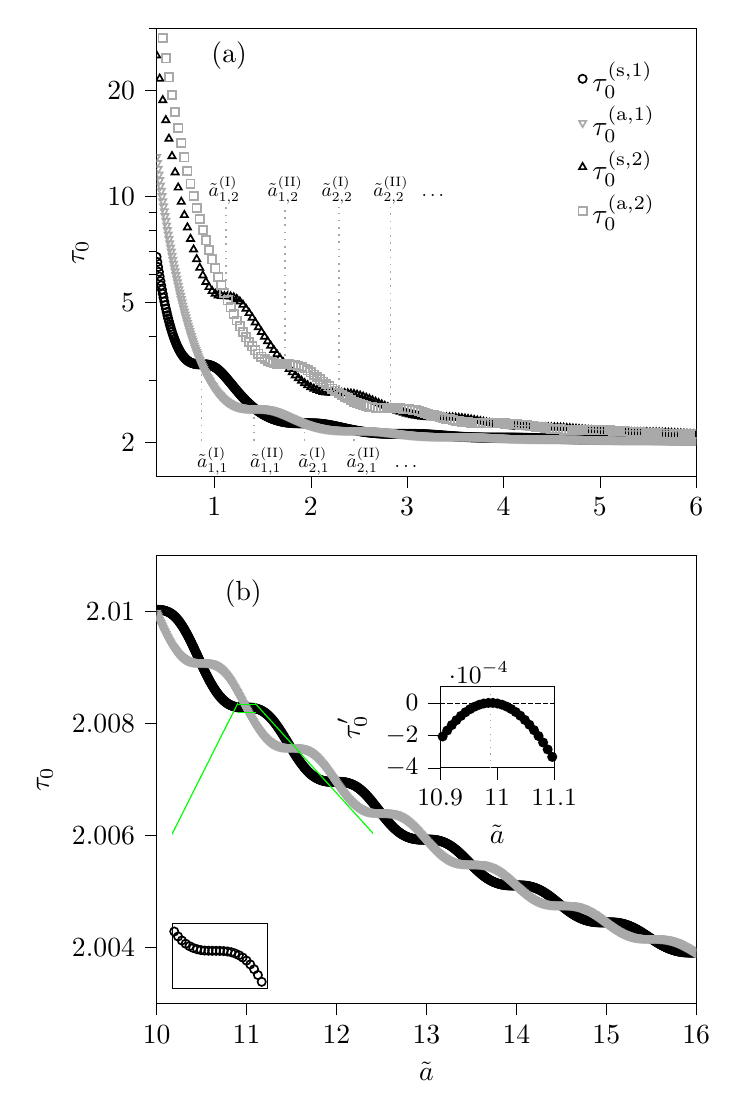
\begin{tikzpicture}

\definecolor{darkgray}{RGB}{169,169,169}
\definecolor{darkgray176}{RGB}{176,176,176}
\definecolor{lightgray204}{RGB}{204,204,204}

\begin{groupplot}[group style={group size=1 by 2},clip marker paths=true]
\nextgroupplot[
legend cell align={left},
legend style={fill opacity=0.8, draw opacity=1, text opacity=1, at={(0.95,0.95)}, draw=none},
log basis y={10},
tick align=outside,
tick pos=left,
x grid style={darkgray176},
xmin=0.4, xmax=6,
xtick style={color=black},
y grid style={darkgray176},
ylabel={\(\displaystyle \tau_0\)},
ymin=1.6, ymax=30,
ymode=log,
ytick style={color=black},
log ticks with fixed point, %afegit a ma
ytick={2,5,10,20}, %afegit a ma
minor ytick={3,4,6,7,8,9,30} %afegit a ma
]
\addplot [semithick, black, mark=o, mark size=1.5, mark options={solid,fill=none}, only marks]
table {%
0.4 6.72825292030247
0.408 6.50472697124453
0.416 6.29542811862217
0.424 6.09931777255341
0.432 5.91545229187631
0.44 5.74297269919318
0.448 5.5810956684581
0.456 5.42910560800124
0.464 5.28634768911461
0.472 5.15222169297914
0.48 5.02617656762402
0.488 4.9077056024444
0.496 4.7963421411059
0.504 4.69165576487054
0.512 4.59324888784717
0.52 4.50075371369173
0.528 4.41382951009721
0.536 4.3321601632177
0.544 4.25545197912645
0.552 4.1834317036493
0.56 4.11584473555358
0.568 4.05245351120064
0.576 3.99303604146579
0.584 3.9373845840565
0.592 3.88530443637343
0.6 3.83661283580419
0.608 3.79113795585573
0.616 3.7487179878511
0.624 3.70920029906621
0.632 3.67244065918824
0.64 3.63830252785762
0.648 3.6066563968287
0.656 3.57737918096583
0.664 3.55035365289329
0.672 3.52546791665344
0.68 3.50261491620545
0.688 3.48169197502918
0.696 3.46260036349192
0.704 3.44524489099944
0.712 3.42953352029495
0.72 3.41537700159799
0.728 3.40268852459844
0.736 3.39138338664719
0.744 3.38137867582299
0.752 3.37259296791516
0.76 3.36494603675231
0.768 3.35835857774024
0.776 3.35275194495659
0.784 3.34804790269751
0.792 3.34416839299049
0.8 3.34103532128661
0.808 3.33857036332753
0.816 3.33669479704719
0.824 3.33532936430497
0.832 3.33439416823546
0.84 3.33380861300257
0.848 3.33349139370581
0.856 3.33336054502354
0.864 3.33333355778063
0.872 3.33332757285928
0.88 3.33325966156223
0.888 3.33304720050134
0.896 3.33260834712624
0.904 3.33186261895565
0.912 3.33073157530565
0.92 3.32913959480441
0.928 3.32701473536321
0.936 3.32428965585236
0.944 3.32090257103383
0.952 3.31679820406723
0.96 3.31192869502812
0.968 3.30625442031033
0.976 3.29974467739081
0.984 3.29237819281517
0.992 3.28414341859159
1 3.27503859310346
1.008 3.26507155626806
1.016 3.25425932363295
1.024 3.24262743882019
1.032 3.2302091366228
1.04 3.21704435882346
1.048 3.2031786706164
1.056 3.18866212711595
1.064 3.1735481371314
1.072 3.15789236591412
1.08 3.14175171093658
1.088 3.12518337600966
1.096 3.10824406016065
1.104 3.09098926945622
1.112 3.07347275289031
1.12 3.05574605784447
1.128 3.03785819653573
1.136 3.01985541220195
1.144 3.00178103234679
1.152 2.98367539593512
1.16 2.96557584174608
1.168 2.9475167459249
1.176 2.92952959792775
1.184 2.91164310536922
1.192 2.8938833196401
1.2 2.87627377548193
1.208 2.85883563892912
1.216 2.84158785912984
1.224 2.82454732051988
1.232 2.80772899264669
1.24 2.79114607563233
1.248 2.7748101398335
1.256 2.7587312587189
1.264 2.74291813435254
1.272 2.72737821516095
1.28 2.7121178058846
1.288 2.69714216978188
1.296 2.6824556232774
1.304 2.6680616233339
1.312 2.65396284788661
1.32 2.64016126971595
1.328 2.62665822415478
1.336 2.61345447103349
1.344 2.60055025126384
1.352 2.58794533845299
1.36 2.57563908592478
1.368 2.56363046950755
1.376 2.55191812642822
1.384 2.54050039063116
1.392 2.52937532481947
1.4 2.51854074949484
1.408 2.50799426925167
1.416 2.49773329656125
1.424 2.48775507326301
1.432 2.47805668996156
1.44 2.46863510351212
1.448 2.45948715276071
1.456 2.45060957269139
1.464 2.44199900711916
1.472 2.43365202005491
1.48 2.42556510585734
1.488 2.41773469827627
1.496 2.41015717848238
1.504 2.40282888216949
1.512 2.39574610580747
1.52 2.38890511211673
1.528 2.38230213482839
1.536 2.37593338278834
1.544 2.36979504345765
1.552 2.36388328585707
1.56 2.35819426299837
1.568 2.35272411384167
1.576 2.34746896481348
1.584 2.34242493091744
1.592 2.33758811646606
1.6 2.33295461545946
1.608 2.32852051163428
1.616 2.32428187820386
1.624 2.32023477730878
1.632 2.316375259195
1.64 2.31269936113546
1.648 2.3092031061096
1.656 2.30588250125413
1.664 2.30273353609766
1.672 2.29975218059092
1.68 2.29693438294397
1.688 2.29427606728169
1.696 2.29177313112851
1.704 2.28942144273404
1.712 2.28721683825132
1.72 2.28515511878069
1.728 2.2832320472929
1.736 2.28144334544693
1.744 2.27978469031944
1.752 2.2782517110652
1.76 2.27683998553009
1.768 2.27554503684175
1.776 2.27436233000581
1.784 2.27328726854022
1.792 2.27231519118428
1.8 2.27144136872421
1.808 2.27066100098259
1.816 2.26996921402544
1.824 2.26936105764695
1.832 2.26883150319974
1.84 2.26837544184565
1.848 2.26798768331059
1.856 2.26766295523513
1.864 2.26739590322102
1.872 2.26718109168218
1.88 2.2670130056165
1.888 2.26688605342221
1.896 2.26679457088841
1.904 2.26673282649373
1.912 2.26669502814935
1.92 2.26667533152177
1.928 2.26666785006669
1.936 2.26666666689641
1.944 2.26666584859005
1.952 2.26665946103594
1.96 2.26664158737033
1.968 2.26660634804295
1.976 2.26654792300059
1.984 2.2664605759317
1.992 2.26633868046093
2 2.26617674812126
2.008 2.26596945786572
2.016 2.2657116868115
2.024 2.26539854183912
2.032 2.26502539160133
2.04 2.26458789843406
2.048 2.26408204960753
2.056 2.26350418731544
2.064 2.26285103677499
2.072 2.26211973180574
2.08 2.26130783727222
2.088 2.26041336781502
2.096 2.2594348023592
2.104 2.25837109397455
2.112 2.25722167476768
2.12 2.25598645560758
2.128 2.25466582061739
2.136 2.25326061650189
2.144 2.25177213691439
2.152 2.25020210219353
2.16 2.24855263491284
2.168 2.24682623178054
2.176 2.24502573249879
2.184 2.24315428623938
2.192 2.24121531641575
2.2 2.23921248442967
2.208 2.23714965304754
2.216 2.23503085001838
2.224 2.23286023248796
2.232 2.23064205269359
2.24 2.22838062534809
2.248 2.22608029704132
2.256 2.22374541790808
2.264 2.22138031573509
2.272 2.21898927260857
2.28 2.21657650414071
2.288 2.21414614125772
2.296 2.21170221448586
2.304 2.20924864063405
2.312 2.2067892117426
2.32 2.2043275861464
2.328 2.20186728148659
2.336 2.19941166949699
2.344 2.19696397238881
2.352 2.19452726065865
2.36 2.19210445215
2.368 2.18969831220607
2.376 2.18731145476106
2.384 2.18494634422811
2.392 2.18260529805346
2.4 2.18029048981812
2.408 2.17800395278039
2.416 2.17574758376365
2.424 2.17352314730533
2.432 2.17133227999277
2.44 2.16917649492177
2.448 2.16705718622216
2.456 2.16497563360305
2.464 2.16293300687746
2.472 2.16093037043278
2.48 2.15896868761904
2.488 2.15704882503243
2.496 2.15517155667565
2.504 2.1533375679808
2.512 2.15154745968379
2.52 2.14980175154224
2.528 2.1481008858912
2.536 2.14644523103319
2.544 2.1448350844609
2.552 2.14327067591218
2.56 2.14175217025838
2.568 2.14027967022796
2.576 2.1388532189681
2.584 2.13747280244788
2.592 2.1361383517068
2.6 2.13484974495311
2.608 2.13360680951658
2.616 2.13240932366048
2.624 2.131257018258
2.632 2.13014957833809
2.64 2.12908664450602
2.648 2.12806781424396
2.656 2.1270926430969
2.664 2.12616064574921
2.672 2.12527129699727
2.68 2.12442403262355
2.688 2.12361825017757
2.696 2.12285330966936
2.704 2.12212853418087
2.712 2.12144321040116
2.72 2.12079658909131
2.728 2.12018788548486
2.736 2.1196162796304
2.744 2.11908091668263
2.752 2.11858090714893
2.76 2.1181153270986
2.768 2.1176832183426
2.776 2.11728358859194
2.784 2.11691541160336
2.792 2.11657762732182
2.8 2.11626914202972
2.808 2.11598882851361
2.816 2.11573552625984
2.824 2.11550804169162
2.832 2.11530514846053
2.84 2.11512558780664
2.848 2.11496806900228
2.856 2.11483126989527
2.864 2.1147138375684
2.872 2.11461438913295
2.88 2.11453151267443
2.888 2.11446376836981
2.896 2.1144096897957
2.904 2.11436778544746
2.912 2.11433654048917
2.92 2.11431441875434
2.928 2.11429986501649
2.936 2.11429130754786
2.944 2.11428716098305
2.952 2.11428582950245
2.96 2.11428571034752
2.968 2.11428519767711
2.976 2.11428268676979
2.984 2.11427657857262
2.992 2.11426528459169
3 2.11424723211327
3.008 2.11422086973823
3.016 2.11418467320469
3.024 2.11413715146644
3.032 2.11407685298637
3.04 2.11400237219614
3.048 2.1139123560652
3.056 2.11380551071437
3.064 2.1136806080023
3.072 2.11353649200674
3.08 2.11337208531778
3.088 2.11318639505667
3.096 2.11297851853217
3.104 2.1127476484469
3.112 2.11249307756859
3.12 2.112214202786
3.128 2.11191052847653
3.136 2.11158166912153
3.144 2.11122735111703
3.152 2.1108474137403
3.16 2.11044180924731
3.168 2.11001060209129
3.176 2.10955396726847
3.184 2.1090721878128
3.192 2.10856565147652
3.2 2.10803484664758
3.208 2.10748035756744
3.216 2.10690285892357
3.224 2.10630310989955
3.232 2.10568194777181
3.24 2.10504028114617
3.248 2.10437908292852
3.256 2.10369938312351
3.264 2.10300226155194
3.272 2.10228884057304
3.28 2.10156027789147
3.288 2.10081775952146
3.296 2.10006249297207
3.304 2.09929570070852
3.312 2.09851861393579
3.32 2.09773246674086
3.328 2.09693849062161
3.336 2.09613790942179
3.344 2.09533193468344
3.352 2.09452176142137
3.36 2.09370856431782
3.368 2.09289349433
3.376 2.09207767569857
3.384 2.09126220334158
3.392 2.0904481406149
3.4 2.08963651741847
3.408 2.08882832862578
3.416 2.08802453281288
3.424 2.08722605126322
3.432 2.0864337672239
3.44 2.08564852538979
3.448 2.08487113159243
3.456 2.08410235267125
3.464 2.08334291650607
3.472 2.08259351219079
3.48 2.08185479032943
3.488 2.0811273634372
3.496 2.08041180643034
3.504 2.07970865719002
3.512 2.07901841718681
3.52 2.07834155215348
3.528 2.07767849279516
3.536 2.07702963552704
3.544 2.0763953432307
3.552 2.07577594602152
3.56 2.07517174202013
3.568 2.07458299812218
3.576 2.07400995076112
3.584 2.07345280665953
3.592 2.07291174356549
3.6 2.07238691097054
3.608 2.07187843080683
3.616 2.07138639812129
3.624 2.07091088172512
3.632 2.07045192481747
3.64 2.07000954558228
3.648 2.06958373775782
3.656 2.06917447117867
3.664 2.06878169229014
3.672 2.06840532463543
3.68 2.068045269316
3.688 2.06770140542596
3.696 2.06737359046127
3.704 2.0670616607051
3.712 2.06676543159039
3.72 2.06648469804133
3.728 2.06621923479534
3.736 2.06596879670739
3.744 2.06573311903879
3.752 2.06551191773254
3.76 2.06530488967781
3.768 2.06511171296598
3.776 2.06493204714123
3.784 2.06476553344853
3.792 2.06461179508238
3.8 2.06447043743968
3.808 2.06434104838045
3.816 2.06422319850022
3.824 2.06411644141838
3.832 2.06402031408667
3.84 2.06393433712261
3.848 2.06385801517253
3.856 2.06379083730936
3.864 2.06373227747032
3.872 2.06368179494003
3.88 2.06363883488448
3.888 2.06360282894161
3.896 2.06357319587416
3.904 2.06354934229056
3.912 2.06353066343949
3.92 2.06351654408356
3.928 2.0635063594575
3.936 2.0634994763157
3.944 2.06349525407358
3.952 2.06349304604669
3.96 2.06349220079073
3.968 2.06349206354477
3.976 2.06349197777898
3.984 2.06349128684684
3.992 2.06348933574087
4 2.06348547294887
4.008 2.06347905240652
4.016 2.06346943554007
4.024 2.06345599339123
4.032 2.06343810881427
4.04 2.06341517873328
4.048 2.06338661644569
4.056 2.06335185395594
4.064 2.06331034432156
4.072 2.06326156399179
4.08 2.06320501511775
4.088 2.06314022781145
4.096 2.06306676233024
4.104 2.06298421116264
4.112 2.06289220099112
4.12 2.06279039450801
4.128 2.06267849206109
4.136 2.06255623310714
4.144 2.06242339745298
4.152 2.06227980626628
4.16 2.0621253228407
4.168 2.06195985310331
4.176 2.06178334585555
4.184 2.0615957927425
4.192 2.06139722794947
4.2 2.06118772762824
4.208 2.06096740905965
4.216 2.06073642956263
4.224 2.06049498516323
4.232 2.06024330904064
4.24 2.05998166976947
4.248 2.05971036938043
4.256 2.05942974126279
4.264 2.05914014793373
4.272 2.05884197870027
4.28 2.05853564723963
4.288 2.05822158912386
4.296 2.05790025931359
4.304 2.057572129645
4.312 2.05723768633227
4.32 2.05689742750633
4.328 2.05655186080864
4.336 2.05620150105669
4.344 2.05584686799548
4.352 2.05548848414744
4.36 2.05512687277048
4.368 2.05476255593208
4.376 2.05439605270509
4.384 2.0540278774891
4.392 2.05365853845915
4.4 2.05328853614236
4.408 2.05291836212133
4.416 2.0525484978618
4.424 2.05217941366155
4.432 2.05181156771581
4.44 2.05144540529446
4.448 2.05108135802532
4.456 2.05071984327751
4.464 2.05036126363862
4.472 2.05000600647921
4.48 2.04965444359811
4.488 2.04930693094205
4.496 2.04896380839314
4.504 2.04862539961798
4.512 2.04829201197248
4.52 2.0479639364564
4.528 2.04764144771227
4.536 2.04732480406346
4.544 2.04701424758644
4.552 2.04671000421288
4.56 2.04641228385709
4.568 2.04612128056517
4.576 2.04583717268212
4.584 2.04556012303377
4.592 2.0452902791205
4.6 2.04502777332013
4.608 2.04477272309761
4.616 2.04452523121934
4.624 2.04428538597031
4.632 2.04405326137247
4.64 2.04382891740275
4.648 2.04361240020986
4.656 2.04340374232848
4.664 2.04320296289043
4.672 2.0430100678319
4.68 2.04282505009644
4.688 2.04264788983332
4.696 2.04247855459118
4.704 2.04231699950696
4.712 2.04216316749007
4.72 2.04201698940235
4.728 2.04187838423389
4.736 2.04174725927545
4.744 2.04162351028799
4.752 2.04150702166999
4.76 2.04139766662363
4.768 2.04129530732049
4.776 2.04119979506814
4.784 2.04111097047856
4.792 2.04102866363988
4.8 2.04095269429266
4.808 2.04088287201239
4.816 2.04081899639965
4.824 2.04076085727979
4.832 2.04070823491376
4.84 2.04066090022218
4.848 2.04061861502441
4.856 2.04058113229491
4.864 2.04054819643871
4.872 2.04051954358846
4.88 2.04049490192502
4.888 2.04047399202395
4.896 2.04045652723003
4.904 2.04044221406207
4.912 2.04043075265012
4.92 2.04042183720701
4.928 2.04041515653641
4.936 2.04041039457887
4.944 2.04040723099763
4.952 2.04040534180535
4.96 2.04040440003294
4.968 2.04040407644104
4.976 2.04040404027444
4.984 2.04040396005934
4.992 2.04040350444269
5 2.04040234307249
5.008 2.04040014751707
5.016 2.04039659222102
5.024 2.04039135549466
5.032 2.04038412053303
5.04 2.04037457646003
5.048 2.04036241939233
5.056 2.04034735351707
5.064 2.04032909217675
5.072 2.0403073589538
5.08 2.04028188874712
5.088 2.040252428832
5.096 2.0402187398947
5.104 2.04018059703242
5.112 2.04013779070949
5.12 2.04009012766023
5.128 2.04003743172946
5.136 2.03997954464149
5.144 2.03991632668933
5.152 2.03984765733592
5.16 2.03977343572051
5.168 2.03969358106389
5.176 2.03960803296716
5.184 2.03951675160037
5.192 2.03941971777795
5.2 2.03931693291978
5.208 2.03920841889778
5.216 2.0390942177693
5.224 2.03897439140015
5.232 2.03884902098117
5.24 2.03871820644361
5.248 2.03858206577966
5.256 2.0384407342755
5.264 2.03829436366504
5.272 2.03814312121328
5.28 2.0379871887386
5.288 2.0378267615839
5.296 2.03766204754635
5.304 2.03749326577583
5.312 2.03732064565185
5.32 2.03714442564844
5.328 2.03696485219615
5.336 2.03678217854974
5.344 2.0365966636696
5.352 2.03640857112409
5.36 2.03621816801938
5.368 2.03602572396267
5.376 2.03583151006354
5.384 2.03563579797794
5.392 2.03543885899791
5.4 2.03524096318993
5.408 2.03504237858372
5.416 2.03484337041282
5.424 2.03464420040763
5.432 2.03444512614092
5.44 2.03424640042555
5.448 2.03404827076341
5.456 2.03385097884448
5.464 2.03365476009437
5.472 2.03345984326853
5.48 2.03326645009117
5.488 2.03307479493657
5.496 2.03288508455053
5.504 2.03269751780955
5.512 2.03251228551527
5.52 2.03232957022162
5.528 2.03214954609246
5.536 2.03197237878701
5.544 2.03179822537093
5.552 2.03162723425072
5.56 2.03145954512915
5.568 2.03129528897987
5.576 2.03113458803892
5.584 2.03097755581158
5.592 2.03082429709258
5.6 2.03067490799822
5.608 2.0305294760088
5.616 2.03038808002002
5.624 2.03025079040209
5.632 2.03011766906543
5.64 2.02998876953189
5.648 2.02986413701064
5.656 2.02974380847788
5.664 2.02962781275969
5.672 2.02951617061745
5.68 2.02940889483526
5.688 2.0293059903091
5.696 2.0292074541372
5.704 2.0291132757117
5.712 2.02902343681108
5.72 2.02893791169373
5.728 2.02885666719226
5.736 2.02877966280903
5.744 2.02870685081277
5.752 2.02863817633674
5.76 2.02857357747862
5.768 2.02851298540262
5.776 2.02845632444412
5.784 2.02840351221749
5.792 2.02835445972761
5.8 2.0283090714857
5.808 2.02826724563016
5.816 2.02822887405322
5.824 2.02819384253411
5.832 2.0281620308797
5.84 2.02813331307334
5.848 2.02810755743306
5.856 2.02808462677981
5.864 2.028064378617
5.872 2.02804666532208
5.88 2.02803133435144
5.888 2.02801822845942
5.896 2.02800718593253
5.904 2.02799804083991
5.912 2.02799062330085
5.92 2.02798475977036
5.928 2.02798027334354
5.936 2.0279769840796
5.944 2.02797470934596
5.952 2.02797326418312
5.96 2.02797246169059
5.968 2.02797211343405
5.976 2.02797202987368
5.984 2.0279720208136
5.992 2.02797189587186
6 2.02797146497024
6.008 2.02797053884298
6.016 2.02796892956312
6.024 2.02796645108492
6.032 2.02796291980038
6.04 2.02795815510779
6.048 2.02795197998968
6.056 2.02794422159744
6.064 2.02793471183934
6.072 2.02792328796863
6.08 2.027909793168
6.088 2.02789407712641
6.096 2.02787599660432
6.104 2.02785541598285
6.112 2.02783220779275
6.12 2.02780625321849
6.128 2.0277774425734
6.136 2.02774567574127
6.144 2.02771086258049
6.152 2.02767292328665
6.16 2.02763178871012
6.168 2.02758740062518
6.176 2.02753971194796
6.184 2.02748868690075
6.192 2.02743430112087
6.2 2.02737654171264
6.208 2.02731540724198
6.216 2.02725090767324
6.224 2.02718306424896
6.232 2.02711190931352
6.24 2.02703748608243
6.248 2.02695984835945
6.256 2.02687906020427
6.264 2.026795195554
6.272 2.02670833780207
6.28 2.02661857933852
6.288 2.02652602105591
6.296 2.0264307718253
6.304 2.026332947947
6.312 2.02623267258056
6.32 2.0261300751589
6.328 2.02602529079099
6.336 2.02591845965772
6.344 2.02580972640512
6.352 2.02569923953913
6.36 2.02558715082571
6.368 2.02547361469977
6.376 2.02535878768617
6.384 2.02524282783569
6.392 2.02512589417843
6.4 2.02500814619693
6.408 2.02488974332063
6.416 2.02477084444351
6.424 2.02465160746567
6.432 2.02453218886013
6.44 2.02441274326503
6.448 2.02429342310186
6.456 2.02417437821957
6.464 2.02405575556448
6.472 2.02393769887566
6.48 2.02382034840512
6.488 2.02370384066236
6.496 2.02358830818224
6.504 2.02347387931541
6.512 2.02336067804031
6.52 2.02324882379569
6.528 2.02313843133243
6.536 2.02302961058385
6.544 2.02292246655303
6.552 2.02281709921627
6.56 2.0227136034415
6.568 2.02261206892045
6.576 2.02251258011369
6.584 2.02241521620737
6.592 2.02232005108074
6.6 2.0222271532835
6.608 2.02213658602208
6.616 2.022048407154
6.624 2.02196266918965
6.632 2.02187941930052
6.64 2.02179869933353
6.648 2.02172054583053
6.656 2.02164499005276
6.664 2.02157205800941
6.672 2.02150177049023
6.68 2.02143414310146
6.688 2.021369186305
6.696 2.02130690546047
6.704 2.02124730086995
6.712 2.02119036782516
6.72 2.02113609665711
6.728 2.0210844727881
6.736 2.02103547678593
6.744 2.02098908442056
6.752 2.02094526672312
6.76 2.02090399004751
6.768 2.02086521613464
6.776 2.02082890217957
6.784 2.02079500090185
6.792 2.02076346061916
6.8 2.02073422532476
6.808 2.02070723476896
6.816 2.02068242454508
6.824 2.02065972618016
6.832 2.02063906723109
6.84 2.02062037138639
6.848 2.02060355857418
6.856 2.02058854507698
6.864 2.02057524365359
6.872 2.02056356366881
6.88 2.02055341123127
6.888 2.02054468934018
6.896 2.02053729804118
6.904 2.02053113459199
6.912 2.02052609363829
6.92 2.02052206740017
6.928 2.02051894586954
6.936 2.02051661701901
6.944 2.02051496702223
6.952 2.02051388048611
6.96 2.02051324069494
6.968 2.02051292986645
6.976 2.02051282941968
6.984 2.02051282025462
6.992 2.02051278304307
7 2.02051259853043
7.008 2.0205121478478
7.016 2.02051131283357
7.024 2.02050997636365
7.032 2.02050802268926
7.04 2.02050533778108
7.048 2.02050180967824
7.056 2.02049732884082
7.064 2.02049178850393
7.072 2.02048508503165
7.08 2.02047711826876
7.088 2.02046779188828
7.096 2.02045701373246
7.104 2.02044469614501
7.112 2.02043075629227
7.12 2.02041511647091
7.128 2.02039770439975
7.136 2.02037845349349
7.144 2.020357303116
7.152 2.02033419881101
7.16 2.02030909250827
7.168 2.02028194270315
7.176 2.02025271460821
7.184 2.02022138027509
7.192 2.02018791868579
7.2 2.02015231581211
7.208 2.02011456464289
7.216 2.02007466517857
7.224 2.0200326243931
7.232 2.01998845616345
7.24 2.01994218116742
7.248 2.01989382675045
7.256 2.01984342676284
7.264 2.01979102136861
7.272 2.01973665682785
7.28 2.01968038525435
7.288 2.01962226435062
7.296 2.01956235712254
7.304 2.01950073157604
7.312 2.01943746039816
7.32 2.01937262062502
7.328 2.01930629329924
7.336 2.01923856311924
7.344 2.01916951808291
7.352 2.019099249128
7.36 2.01902784977152
7.368 2.01895541575025
7.376 2.0188820446645
7.384 2.01880783562684
7.392 2.01873288891762
7.4 2.01865730564873
7.408 2.01858118743703
7.416 2.01850463608857
7.424 2.01842775329461
7.432 2.01835064034037
7.44 2.01827339782701
7.448 2.0181961254075
7.456 2.01811892153662
7.464 2.01804188323545
7.472 2.01796510587027
7.48 2.01788868294602
7.488 2.01781270591398
7.496 2.01773726399371
7.504 2.01766244400871
7.512 2.01758833023555
7.52 2.01751500426602
7.528 2.01744254488176
7.536 2.01737102794101
7.544 2.01730052627667
7.552 2.01723110960542
7.56 2.01716284444708
7.568 2.0170957940537
7.576 2.01703001834786
7.584 2.01696557386952
7.592 2.01690251373092
7.6 2.01684088757894
7.608 2.01678074156441
7.616 2.01672211831787
7.624 2.01666505693129
7.632 2.01660959294533
7.64 2.01655575834162
7.648 2.01650358153984
7.656 2.01645308739906
7.664 2.01640429722307
7.672 2.0163572287695
7.68 2.01631189626232
7.688 2.01626831040754
7.696 2.01622647841195
7.704 2.01618640400469
7.712 2.01614808746151
7.72 2.01611152563164
7.728 2.01607671196716
7.736 2.01604363655487
7.744 2.01601228615058
7.752 2.01598264421592
7.76 2.01595469095765
7.768 2.01592840336946
7.776 2.0159037552766
7.784 2.01588071738317
7.792 2.01585925732235
7.8 2.0158393397098
7.808 2.01582092620028
7.816 2.0158039755477
7.824 2.01578844366899
7.832 2.0157742837118
7.84 2.01576144612642
7.848 2.01574987874221
7.856 2.01573952684862
7.864 2.01573033328133
7.872 2.01572223851361
7.88 2.01571518075322
7.888 2.01570909604519
7.896 2.01570391838061
7.904 2.01569957981191
7.912 2.01569601057456
7.92 2.01569313921568
7.928 2.01569089272963
7.936 2.0156891967007
7.944 2.01568797545308
7.952 2.01568715220819
7.96 2.0156866492493
7.968 2.0156863880935
7.976 2.01568628967094
7.984 2.01568627451101
7.992 2.01568626293545
8 2.0156861752579
8.008 2.01568593198954
8.016 2.01568545405041
8.024 2.0156846629857
8.032 2.01568348118646
8.04 2.0156818321139
8.048 2.01567964052648
8.056 2.01567683270879
8.064 2.01567333670128
8.072 2.01566908252963
8.08 2.01566400243267
8.088 2.01565803108755
8.096 2.01565110583085
8.104 2.01564316687435
8.112 2.01563415751398
8.12 2.01562402433066
8.128 2.01561271738151
8.136 2.0156001903802
8.144 2.01558640086498
8.152 2.01557131035314
8.16 2.01555488448069
8.168 2.01553709312606
8.176 2.01551791051693
8.184 2.01549731531911
8.192 2.01547529070679
8.2 2.01545182441358
8.208 2.01542690876374
8.216 2.0154005406834
8.224 2.01537272169164
8.232 2.0153434578714
8.24 2.01531275982055
8.248 2.01528064258336
8.256 2.01524712556314
8.264 2.01521223241655
8.272 2.01517599093059
8.28 2.01513843288323
8.288 2.01509959388878
8.296 2.01505951322925
8.304 2.015018233673
8.312 2.01497580128208
8.32 2.01493226520961
8.328 2.01488767748886
8.336 2.01484209281519
8.344 2.01479556832265
8.352 2.01474816335648
8.36 2.01469993924296
8.368 2.01465095905801
8.376 2.01460128739587
8.384 2.01455099013896
8.392 2.01450013423021
8.4 2.01444878744884
8.408 2.01439701819056
8.416 2.01434489525303
8.424 2.01429248762749
8.432 2.01423986429698
8.44 2.01418709404197
8.448 2.01413424525371
8.456 2.01408138575573
8.464 2.01402858263382
8.472 2.01397590207467
8.48 2.01392340921322
8.488 2.01387116798898
8.496 2.01381924101112
8.504 2.01376768943232
8.512 2.01371657283136
8.52 2.01366594910416
8.528 2.01361587436309
8.536 2.01356640284444
8.544 2.01351758682361
8.552 2.01346947653778
8.56 2.01342212011595
8.568 2.01337556351565
8.576 2.01332985046645
8.584 2.01328502241951
8.592 2.01324111850324
8.6 2.01319817548437
8.608 2.01315622773446
8.616 2.01311530720123
8.624 2.01307544338472
8.632 2.01303666331767
8.64 2.0129989915501
8.648 2.01296245013777
8.656 2.01292705863419
8.664 2.01289283408605
8.672 2.01285979103187
8.68 2.01282794150361
8.688 2.01279729503119
8.696 2.01276785864965
8.704 2.01273963690892
8.712 2.01271263188605
8.72 2.01268684319985
8.728 2.01266226802782
8.736 2.01263890112537
8.744 2.01261673484729
8.752 2.01259575917145
8.76 2.01257596172477
8.768 2.01255732781143
8.776 2.01253984044344
8.784 2.01252348037355
8.792 2.01250822613062
8.8 2.01249405405758
8.808 2.01248093835196
8.816 2.0124688511092
8.824 2.01245776236894
8.832 2.01244764016415
8.84 2.01243845057359
8.848 2.01243015777752
8.856 2.01242272411688
8.864 2.01241611015609
8.872 2.01241027474966
8.88 2.0124051751128
8.888 2.01240076689599
8.896 2.01239700426397
8.904 2.012393839979
8.912 2.01239122548867
8.92 2.01238911101837
8.928 2.01238744566846
8.936 2.01238617751618
8.944 2.01238525372251
8.952 2.01238462064375
8.96 2.01238422394804
8.968 2.01238400873663
8.976 2.01238391966978
8.984 2.01238390109735
8.992 2.01238389719363
9 2.01238385209638
9.008 2.01238371004973
9.016 2.01238341555062
9.024 2.01238291349835
9.032 2.0123821493468
9.04 2.01238106925895
9.048 2.01237962026291
9.056 2.01237775040907
9.064 2.01237540892756
9.072 2.01237254638536
9.08 2.01236911484236
9.088 2.01236506800547
9.096 2.01236036138001
9.104 2.01235495241756
9.112 2.01234880065926
9.12 2.01234186787392
9.128 2.01233411818972
9.136 2.01232551821901
9.144 2.012316037175
9.152 2.01230564697974
9.16 2.01229432236258
9.168 2.01228204094822
9.176 2.01226878333396
9.184 2.01225453315521
9.192 2.01223927713906
9.2 2.01222300514527
9.208 2.01220571019437
9.216 2.01218738848278
9.224 2.01216803938456
9.232 2.01214766544004
9.24 2.01212627233113
9.248 2.01210386884376
9.256 2.01208046681754
9.264 2.01205608108312
9.272 2.01203072938767
9.28 2.01200443230917
9.288 2.01197721316003
9.296 2.01194909788079
9.304 2.01192011492478
9.312 2.01189029513442
9.32 2.01185967161016
9.328 2.01182827957292
9.336 2.01179615622093
9.344 2.01176334058196
9.352 2.01172987336178
9.36 2.01169579678986
9.368 2.01166115446316
9.376 2.01162599118888
9.384 2.01159035282699
9.392 2.01155428613333
9.4 2.01151783860408
9.408 2.01148105832217
9.416 2.01144399380636
9.424 2.0114066938635
9.432 2.01136920744454
9.44 2.0113315835047
9.448 2.01129387086813
9.456 2.01125611809758
9.464 2.01121837336916
9.472 2.01118068435248
9.48 2.01114309809644
9.488 2.01110566092054
9.496 2.01106841831211
9.504 2.01103141482919
9.512 2.01099469400928
9.52 2.01095829828372
9.528 2.01092226889783
9.536 2.01088664583658
9.544 2.01085146775561
9.552 2.01081677191772
9.56 2.01078259413431
9.568 2.01074896871193
9.576 2.0107159284035
9.584 2.01068350436423
9.592 2.01065172611186
9.6 2.01062062149113
9.608 2.01059021664228
9.616 2.01056053597335
9.624 2.01053160213612
9.632 2.01050343600546
9.64 2.01047605666202
9.648 2.01044948137796
9.656 2.01042372560565
9.664 2.01039880296913
9.672 2.0103747252583
9.68 2.01035150242556
9.688 2.01032914258487
9.696 2.01030765201321
9.704 2.01028703515411
9.712 2.01026729462347
9.72 2.01024843121737
9.728 2.0102304439219
9.736 2.01021332992504
9.744 2.01019708463044
9.752 2.01018170167314
9.76 2.01016717293729
9.768 2.01015348857576
9.776 2.01014063703174
9.784 2.01012860506233
9.792 2.01011737776417
9.8 2.0101069386012
9.808 2.0100972694345
9.816 2.01008835055439
9.824 2.01008016071485
9.832 2.01007267717021
9.84 2.01006587571442
9.848 2.01005973072277
9.856 2.01005421519635
9.864 2.0100493008091
9.872 2.01004495795784
9.88 2.01004115581515
9.888 2.01003786238521
9.896 2.01003504456286
9.904 2.01003266819573
9.912 2.01003069814963
9.92 2.01002909837726
9.928 2.01002783199026
9.936 2.01002686133461
9.944 2.01002614806942
9.952 2.01002565324913
9.96 2.01002533740895
9.968 2.01002516065372
9.976 2.01002508274989
9.984 2.01002506322058
9.992 2.0100250614437
10 2.01002503675271
10.008 2.01002494854005
10.016 2.01002475636291
10.024 2.01002442005095
10.032 2.01002389981592
10.04 2.01002315636252
10.048 2.01002215100039
10.056 2.01002084575664
10.064 2.01001920348847
10.072 2.01001718799558
10.08 2.01001476413158
10.088 2.01001189791413
10.096 2.01000855663302
10.104 2.01000470895586
10.112 2.01000032503055
10.12 2.00999537658414
10.128 2.00998983701734
10.136 2.00998368149421
10.144 2.00997688702639
10.152 2.00996943255132
10.16 2.00996129900398
10.168 2.00995246938153
10.176 2.00994292880057
10.184 2.00993266454644
10.192 2.00992166611432
10.2 2.00990992524172
10.208 2.00989743593222
10.216 2.00988419447018
10.224 2.00987019942639
10.232 2.00985545165452
10.24 2.00983995427846
10.248 2.00982371267064
10.256 2.00980673442138
10.264 2.00978902929971
10.272 2.00977060920566
10.28 2.00975148811466
10.288 2.00973168201416
10.296 2.00971120883324
10.304 2.00969008836536
10.312 2.0096683421851
10.32 2.0096459935592
10.328 2.00962306735267
10.336 2.00959958993048
10.344 2.00957558905546
10.352 2.00955109378305
10.36 2.0095261343535
10.368 2.00950074208219
10.376 2.00947494924855
10.384 2.00944878898426
10.392 2.00942229516126
10.4 2.00939550228008
10.408 2.00936844535898
10.416 2.0093411598244
10.424 2.00931368140311
10.432 2.00928604601648
10.44 2.00925828967717
10.448 2.00923044838863
10.456 2.00920255804761
10.464 2.00917465434996
10.472 2.00914677269991
10.48 2.00911894812299
10.488 2.0090912151827
10.496 2.00906360790105
10.504 2.00903615968305
10.512 2.00900890324516
10.52 2.00898187054769
10.528 2.00895509273123
10.536 2.00892860005695
10.544 2.00890242185084
10.552 2.00887658645173
10.56 2.00885112116309
10.568 2.00882605220845
10.576 2.00880140469034
10.584 2.00877720255274
10.592 2.00875346854678
10.6 2.00873022419965
10.608 2.00870748978663
10.616 2.00868528430605
10.624 2.0086636254571
10.632 2.00864252962028
10.64 2.00862201184063
10.648 2.00860208581324
10.656 2.00858276387128
10.664 2.00856405697627
10.672 2.00854597471052
10.68 2.00852852527168
10.688 2.00851171546931
10.696 2.00849555072338
10.704 2.00848003506465
10.712 2.00846517113686
10.72 2.00845096020072
10.728 2.00843740213957
10.736 2.0084244954668
10.744 2.00841223733492
10.752 2.00840062354627
10.76 2.0083896485654
10.768 2.00837930553309
10.776 2.00836958628204
10.784 2.00836048135423
10.792 2.00835198001999
10.8 2.00834407029878
10.808 2.0083367389817
10.816 2.00832997165591
10.824 2.00832375273077
10.832 2.00831806546594
10.84 2.00831289200144
10.848 2.00830821338966
10.856 2.00830400962952
10.864 2.00830025970261
10.872 2.00829694161166
10.88 2.00829403242112
10.888 2.00829150830006
10.896 2.00828934456741
10.904 2.00828751573958
10.912 2.00828599558044
10.92 2.00828475715379
10.928 2.00828377287825
10.936 2.00828301458462
10.944 2.00828245357574
10.952 2.00828206068867
10.96 2.00828180635942
10.968 2.00828166068994
10.976 2.00828159351739
10.984 2.00828157448563
10.992 2.00828157311878
11 2.00828155889672
11.008 2.00828150133237
11.016 2.00828137005057
11.024 2.0082811348684
11.032 2.00828076587665
11.04 2.00828023352216
11.048 2.00827950869093
11.056 2.00827856279145
11.064 2.00827736783811
11.072 2.00827589653431
11.08 2.00827412235485
11.088 2.00827201962726
11.096 2.00826956361176
11.104 2.00826673057928
11.112 2.00826349788725
11.12 2.00825984405278
11.128 2.00825574882269
11.136 2.00825119324006
11.144 2.00824615970693
11.152 2.00824063204269
11.16 2.00823459553783
11.168 2.00822803700271
11.176 2.008220944811
11.184 2.00821330893749
11.192 2.00820512099007
11.2 2.00819637423561
11.208 2.00818706361952
11.216 2.00817718577892
11.224 2.00816673904935
11.232 2.00815572346482
11.24 2.00814414075136
11.248 2.00813199431403
11.256 2.00811928921748
11.264 2.00810603216025
11.272 2.0080922314429
11.28 2.00807789693026
11.288 2.00806304000809
11.296 2.0080476735343
11.304 2.00803181178521
11.312 2.00801547039717
11.32 2.00799866630383
11.328 2.00798141766958
11.336 2.00796374381949
11.344 2.00794566516622
11.352 2.00792720313428
11.36 2.0079083800822
11.368 2.00788921922281
11.376 2.0078697445423
11.384 2.00784998071833
11.392 2.00782995303763
11.4 2.00780968731345
11.408 2.00778920980329
11.416 2.00776854712717
11.424 2.00774772618684
11.432 2.00772677408617
11.44 2.00770571805305
11.448 2.00768458536295
11.456 2.00766340326451
11.464 2.00764219890719
11.472 2.00762099927132
11.48 2.00759983110051
11.488 2.00757872083671
11.496 2.00755769455791
11.504 2.0075367779186
11.512 2.00751599609305
11.52 2.00749537372135
11.528 2.00747493485844
11.536 2.00745470292586
11.544 2.00743470066646
11.552 2.00741495010184
11.56 2.0073954724926
11.568 2.00737628830136
11.576 2.00735741715839
11.584 2.0073388778299
11.592 2.00732068818886
11.6 2.00730286518828
11.608 2.00728542483693
11.616 2.00726838217729
11.624 2.00725175126584
11.632 2.00723554515545
11.64 2.00721977587987
11.648 2.00720445444019
11.656 2.00718959079333
11.664 2.00717519384227
11.672 2.0071612714282
11.68 2.00714783032428
11.688 2.00713487623117
11.696 2.00712241377417
11.704 2.00711044650188
11.712 2.00709897688648
11.72 2.00708800632541
11.728 2.00707753514462
11.736 2.00706756260318
11.744 2.00705808689933
11.752 2.00704910517798
11.76 2.00704061353957
11.768 2.0070326070503
11.776 2.00702507975385
11.784 2.00701802468441
11.792 2.00701143388118
11.8 2.00700529840431
11.808 2.00699960835226
11.816 2.00699435288068
11.824 2.00698952022278
11.832 2.00698509771124
11.84 2.00698107180169
11.848 2.0069774280978
11.856 2.00697415137802
11.864 2.00697122562397
11.872 2.00696863405055
11.88 2.00696635913784
11.888 2.00696438266465
11.896 2.00696268574404
11.904 2.00696124886051
11.912 2.0069600519091
11.92 2.00695907423638
11.928 2.0069582946832
11.936 2.00695769162938
11.944 2.00695724304021
11.952 2.00695692651475
11.96 2.00695671933594
11.968 2.00695659852242
11.976 2.00695654088207
11.984 2.00695652306707
11.992 2.00695652163057
12 2.00695651308468
12.008 2.00695647395977
12.016 2.00695638086496
12.024 2.00695621054952
12.032 2.00695593996515
12.04 2.00695554632886
12.048 2.00695500718626
12.056 2.00695430047511
12.064 2.00695340458874
12.072 2.00695229843927
12.08 2.00695096152025
12.088 2.00694937396843
12.096 2.0069475166245
12.104 2.00694537109239
12.112 2.00694291979685
12.12 2.00694014603909
12.128 2.00693703405008
12.136 2.0069335690413
12.144 2.00692973725259
12.152 2.00692552599685
12.16 2.0069209237013
12.168 2.00691591994511
12.176 2.00691050549308
12.184 2.00690467232515
12.192 2.0068984136617
12.2 2.00689172398427
12.208 2.00688459905167
12.216 2.00687703591144
12.224 2.00686903290636
12.232 2.00686058967622
12.24 2.00685170715471
12.248 2.00684238756137
12.256 2.00683263438887
12.264 2.00682245238549
12.272 2.00681184753305
12.28 2.00680082702037
12.288 2.0067893992125
12.296 2.0067775736158
12.304 2.00676536083927
12.312 2.00675277255222
12.32 2.00673982143859
12.328 2.00672652114831
12.336 2.00671288624576
12.344 2.00669893215587
12.352 2.00668467510806
12.36 2.00667013207828
12.368 2.0066553207296
12.376 2.0066402593515
12.384 2.00662496679829
12.392 2.00660946242694
12.4 2.00659376603453
12.408 2.00657789779563
12.416 2.00656187819998
12.424 2.00654572799048
12.432 2.00652946810204
12.44 2.00651311960116
12.448 2.00649670362672
12.456 2.00648024133201
12.464 2.00646375382817
12.472 2.00644726212925
12.48 2.00643078709894
12.488 2.00641434939911
12.496 2.0063979694403
12.504 2.00638166733408
12.512 2.00636546284754
12.52 2.00634937535978
12.528 2.00633342382058
12.536 2.00631762671109
12.544 2.00630200200672
12.552 2.00628656714214
12.56 2.00627133897838
12.568 2.00625633377197
12.576 2.00624156714625
12.584 2.00622705406456
12.592 2.00621280880552
12.6 2.00619884494021
12.608 2.00618517531121
12.616 2.00617181201353
12.624 2.00615876637728
12.632 2.00614604895212
12.64 2.00613366949334
12.648 2.00612163694966
12.656 2.00610995945246
12.664 2.00609864430674
12.672 2.00608769798337
12.68 2.00607712611293
12.688 2.00606693348086
12.696 2.006057124024
12.704 2.00604770082848
12.712 2.00603866612886
12.72 2.00603002130856
12.728 2.00602176690153
12.736 2.00601390259516
12.744 2.00600642723436
12.752 2.00599933882689
12.76 2.00599263454981
12.768 2.00598631075719
12.776 2.00598036298894
12.784 2.00597478598086
12.792 2.00596957367586
12.8 2.00596471923643
12.808 2.00596021505828
12.816 2.00595605278521
12.824 2.00595222332526
12.832 2.0059487168681
12.84 2.00594552290371
12.848 2.00594263024238
12.856 2.00594002703605
12.864 2.00593770080091
12.872 2.00593563844155
12.88 2.00593382627628
12.888 2.00593225006405
12.896 2.00593089503268
12.904 2.00592974590856
12.912 2.00592878694779
12.92 2.00592800196874
12.928 2.0059273743861
12.936 2.00592688724632
12.944 2.00592652326447
12.952 2.00592626486248
12.96 2.00592609420881
12.968 2.00592599325932
12.976 2.0059259437995
12.984 2.00592592748785
12.992 2.00592592590042
13 2.00592592057637
13.008 2.00592589306449
13.016 2.00592582497055
13.024 2.00592569800538
13.032 2.00592549403353
13.04 2.00592519512235
13.048 2.00592478359139
13.056 2.00592424206189
13.064 2.00592355350617
13.072 2.00592270129687
13.08 2.0059216692556
13.088 2.00592044170106
13.096 2.00591900349618
13.104 2.00591734009425
13.112 2.00591543758371
13.12 2.00591328273139
13.128 2.00591086302404
13.136 2.00590816670786
13.144 2.00590518282584
13.152 2.00590190125269
13.16 2.00589831272724
13.168 2.00589440888198
13.176 2.00589018226965
13.184 2.00588562638676
13.192 2.00588073569377
13.2 2.00587550563195
13.208 2.00586993263668
13.216 2.00586401414719
13.224 2.00585774861265
13.232 2.00585113549458
13.24 2.00584417526555
13.248 2.00583686940419
13.256 2.00582922038655
13.264 2.00582123167378
13.272 2.00581290769644
13.28 2.00580425383518
13.288 2.00579527639831
13.296 2.00578598259606
13.304 2.00577638051191
13.312 2.00576647907109
13.32 2.00575628800643
13.328 2.00574581782173
13.336 2.00573507975301
13.344 2.00572408572769
13.352 2.00571284832197
13.36 2.00570138071674
13.368 2.00568969665213
13.376 2.00567781038099
13.384 2.00566573662151
13.392 2.00565349050924
13.4 2.00564108754864
13.408 2.00562854356453
13.416 2.00561587465344
13.424 2.00560309713523
13.432 2.00559022750503
13.44 2.00557728238583
13.448 2.00556427848162
13.456 2.00555123253152
13.464 2.00553816126484
13.472 2.0055250813572
13.48 2.00551200938794
13.488 2.00549896179874
13.496 2.00548595485367
13.504 2.0054730046007
13.512 2.00546012683465
13.52 2.00544733706172
13.528 2.00543465046563
13.536 2.00542208187531
13.544 2.00540964573421
13.552 2.00539735607132
13.56 2.0053852264737
13.568 2.00537327006071
13.576 2.00536149945982
13.584 2.00534992678398
13.592 2.00533856361064
13.6 2.00532742096218
13.608 2.00531650928798
13.616 2.00530583844788
13.624 2.00529541769712
13.632 2.00528525567266
13.64 2.00527536038092
13.648 2.00526573918681
13.656 2.0052563988041
13.664 2.00524734528704
13.672 2.00523858402319
13.68 2.00523011972753
13.688 2.00522195643765
13.696 2.00521409751016
13.704 2.00520654561816
13.712 2.00519930274988
13.72 2.0051923702083
13.728 2.00518574861191
13.736 2.00517943789647
13.744 2.00517343731782
13.752 2.00516774545569
13.76 2.00516236021854
13.768 2.00515727884938
13.776 2.00515249793265
13.784 2.00514801340204
13.792 2.0051438205494
13.8 2.00513991403455
13.808 2.00513628789626
13.816 2.00513293556412
13.824 2.00512984987155
13.832 2.00512702306985
13.84 2.00512444684323
13.848 2.00512211232506
13.856 2.00512001011508
13.864 2.00511813029782
13.872 2.00511646246207
13.88 2.00511499572147
13.888 2.00511371873633
13.896 2.00511261973648
13.904 2.00511168654533
13.912 2.00511090660508
13.92 2.00511026700307
13.928 2.00510975449925
13.936 2.0051093555548
13.944 2.00510905636185
13.952 2.00510884287433
13.96 2.00510870083978
13.968 2.0051086158323
13.976 2.00510857328637
13.984 2.0051085585317
13.992 2.00510855682881
14 2.00510855340555
14.008 2.00510853349422
14.016 2.00510848236941
14.024 2.00510838538628
14.032 2.00510822801934
14.04 2.00510799590153
14.048 2.00510767486349
14.056 2.00510725097284
14.064 2.00510671057346
14.072 2.00510604032451
14.08 2.00510522723906
14.088 2.00510425872218
14.096 2.00510312260839
14.104 2.00510180719816
14.112 2.00510030129345
14.12 2.005098594232
14.128 2.00509667592027
14.136 2.00509453686483
14.144 2.00509216820205
14.152 2.00508956172593
14.16 2.00508670991394
14.168 2.00508360595061
14.176 2.00508024374896
14.184 2.00507661796939
14.192 2.00507272403612
14.2 2.00506855815097
14.208 2.00506411730443
14.216 2.00505939928395
14.224 2.00505440267942
14.232 2.00504912688579
14.24 2.00504357210274
14.248 2.00503773933161
14.256 2.00503163036935
14.264 2.00502524779971
14.272 2.00501859498163
14.28 2.005011676035
14.288 2.00500449582378
14.296 2.00499705993657
14.304 2.00498937466487
14.312 2.00498144697907
14.32 2.00497328450227
14.328 2.0049648954822
14.336 2.0049562887613
14.344 2.00494747374516
14.352 2.0049384603695
14.36 2.00492925906585
14.368 2.00491988072608
14.376 2.00491033666605
14.384 2.00490063858842
14.392 2.00489079854493
14.4 2.0048808288982
14.408 2.00487074228327
14.416 2.00486055156912
14.424 2.00485026982011
14.432 2.00483991025772
14.44 2.00482948622258
14.448 2.00481901113693
14.456 2.00480849846769
14.464 2.00479796169024
14.472 2.00478741425287
14.48 2.00477686954227
14.488 2.00476634084979
14.496 2.00475584133885
14.504 2.00474538401336
14.512 2.00473498168734
14.52 2.00472464695561
14.528 2.00471439216577
14.536 2.00470422939142
14.544 2.00469417040658
14.552 2.00468422666138
14.56 2.00467440925913
14.568 2.00466472893451
14.576 2.00465519603313
14.584 2.00464582049238
14.592 2.00463661182344
14.6 2.00462757909458
14.608 2.00461873091571
14.616 2.00461007542407
14.624 2.00460162027114
14.632 2.0045933726107
14.64 2.00458533908799
14.648 2.00457752583004
14.656 2.004569938437
14.664 2.00456258197463
14.672 2.0045554609677
14.68 2.00454857939455
14.688 2.00454194068248
14.696 2.00453554770427
14.704 2.0045294027755
14.712 2.00452350765292
14.72 2.00451786353368
14.728 2.00451247105545
14.736 2.00450733029751
14.744 2.0045024407826
14.752 2.00449780147976
14.76 2.00449341080797
14.768 2.00448926664066
14.776 2.00448536631112
14.784 2.00448170661868
14.792 2.0044782838359
14.8 2.00447509371645
14.808 2.00447213150398
14.816 2.00446939194184
14.824 2.00446686928364
14.832 2.00446455730471
14.84 2.00446244931451
14.848 2.00446053816986
14.856 2.00445881628911
14.864 2.00445727566726
14.872 2.00445590789197
14.88 2.00445470416048
14.888 2.00445365529749
14.896 2.00445275177401
14.904 2.00445198372708
14.912 2.00445134098042
14.92 2.0044508130661
14.928 2.00445038924702
14.936 2.00445005854037
14.944 2.00444980974192
14.952 2.00444963145122
14.96 2.00444951209765
14.968 2.0044494399672
14.976 2.00444940323013
14.984 2.00444938996926
14.992 2.00444938820897
15 2.00444938594484
15.008 2.0044493711738
15.016 2.00444933192478
15.024 2.0044492562898
15.032 2.0044491324553
15.04 2.00444894873378
15.048 2.00444869359553
15.056 2.00444835570037
15.064 2.00444792392937
15.072 2.00444738741629
15.08 2.00444673557877
15.088 2.00444595814907
15.096 2.00444504520416
15.104 2.00444398719526
15.112 2.00444277497637
15.12 2.00444139983202
15.128 2.00443985350376
15.136 2.00443812821553
15.144 2.00443621669768
15.152 2.00443411220941
15.16 2.00443180855975
15.168 2.00442930012671
15.176 2.00442658187473
15.184 2.00442364937013
15.192 2.0044204987946
15.2 2.00441712695664
15.208 2.00441353130079
15.216 2.00440970991475
15.224 2.00440566153418
15.232 2.00440138554532
15.24 2.00439688198527
15.248 2.00439215154001
15.256 2.00438719554014
15.264 2.0043820159544
15.272 2.00437661538099
15.28 2.0043709970367
15.288 2.00436516474399
15.296 2.00435912291605
15.304 2.00435287653992
15.312 2.00434643115782
15.32 2.00433979284673
15.328 2.00433296819637
15.336 2.0043259642857
15.344 2.00431878865807
15.352 2.00431144929509
15.36 2.00430395458953
15.368 2.00429631331709
15.376 2.00428853460749
15.384 2.00428062791484
15.392 2.0042726029874
15.4 2.00426446983706
15.408 2.00425623870834
15.416 2.00424792004747
15.424 2.00423952447122
15.432 2.00423106273596
15.44 2.00422254570682
15.448 2.00421398432719
15.456 2.00420538958863
15.464 2.00419677250116
15.472 2.00418814406428
15.48 2.00417951523844
15.488 2.0041708969174
15.496 2.0041622999012
15.504 2.00415373487006
15.512 2.00414521235908
15.52 2.00413674273389
15.528 2.00412833616725
15.536 2.00412000261652
15.544 2.00411175180224
15.552 2.00410359318765
15.56 2.00409553595923
15.568 2.00408758900828
15.576 2.00407976091346
15.584 2.00407205992449
15.592 2.00406449394667
15.6 2.0040570705266
15.608 2.00404979683877
15.616 2.00404267967321
15.624 2.00403572542404
15.632 2.00402894007907
15.64 2.00402232921025
15.648 2.00401589796513
15.656 2.00400965105915
15.664 2.00400359276886
15.672 2.00399772692605
15.68 2.00399205691263
15.688 2.00398658565646
15.696 2.00398131562797
15.704 2.00397624883755
15.712 2.00397138683378
15.72 2.00396673070249
15.728 2.00396228106646
15.736 2.00395803808603
15.744 2.00395400146039
15.752 2.00395017042965
15.76 2.00394654377763
15.768 2.00394311983542
15.776 2.00393989648565
15.784 2.00393687116754
15.792 2.00393404088269
15.8 2.0039314022015
15.808 2.00392895127052
15.816 2.00392668382037
15.824 2.0039245951745
15.832 2.00392268025871
15.84 2.00392093361137
15.848 2.00391934939443
15.856 2.0039179214052
15.864 2.00391664308892
15.872 2.00391550755202
15.88 2.00391450757627
15.888 2.0039136356336
15.896 2.00391288390176
15.904 2.00391224428076
15.912 2.00391170840997
15.92 2.00391126768614
15.928 2.00391091328207
15.936 2.00391063616602
15.944 2.00391042712187
15.952 2.00391027676998
15.96 2.00391017558872
15.968 2.00391011393662
15.976 2.00391008207521
15.984 2.00391007019237
15.992 2.00391006842622
16 2.00391006688955
16.008 2.00391005569462
16.016 2.00391002497838
16.024 2.00390996492799
16.032 2.00390986580658
16.04 2.00390971797916
16.048 2.00390951193866
16.056 2.00390923833197
16.064 2.00390888798586
16.072 2.00390845193274
16.08 2.0039079214362
16.088 2.0039072880161
16.096 2.00390654347328
16.104 2.00390567991356
16.112 2.00390468977124
16.12 2.00390356583168
16.128 2.00390230125302
16.136 2.00390088958694
16.144 2.00389932479832
16.152 2.00389760128369
16.16 2.00389571388842
16.168 2.0038936579225
16.176 2.0038914291749
16.184 2.00388902392638
16.192 2.0038864389607
16.2 2.00388367157417
16.208 2.00388071958344
16.216 2.00387758133161
16.224 2.00387425569246
16.232 2.00387074207289
16.24 2.00386704041355
16.248 2.00386315118759
16.256 2.00385907539764
16.264 2.00385481457088
16.272 2.00385037075244
16.28 2.00384574649699
16.288 2.00384094485861
16.296 2.00383596937913
16.304 2.00383082407476
16.312 2.00382551342137
16.32 2.00382004233818
16.328 2.0038144161703
16.336 2.00380864066993
16.344 2.00380272197645
16.352 2.00379666659546
16.36 2.00379048137697
16.368 2.00378417349266
16.376 2.0037777504125
16.384 2.00377121988076
16.392 2.00376458989152
16.4 2.00375786866375
16.408 2.0037510646162
16.416 2.00374418634201
16.424 2.0037372425833
16.432 2.00373024220577
16.44 2.00372319417334
16.448 2.00371610752308
16.456 2.00370899134031
16.464 2.0037018547341
16.472 2.00369470681318
16.48 2.00368755666228
16.488 2.00368041331907
16.496 2.00367328575163
16.504 2.00366618283659
16.512 2.00365911333792
16.52 2.00365208588647
16.528 2.00364510896018
16.536 2.00363819086513
16.544 2.00363133971733
16.552 2.00362456342536
16.56 2.00361786967375
16.568 2.0036112659073
16.576 2.00360475931613
16.584 2.00359835682159
16.592 2.00359206506306
16.6 2.0035858903855
16.608 2.00357983882789
16.616 2.00357391611244
16.624 2.00356812763466
16.632 2.00356247845416
16.64 2.00355697328635
16.648 2.00355161649479
16.656 2.00354641208442
16.664 2.00354136369546
16.672 2.0035364745981
16.68 2.00353174768792
16.688 2.00352718548199
16.696 2.00352279011575
16.704 2.00351856334049
16.712 2.0035145065216
16.72 2.00351062063747
16.728 2.00350690627904
16.736 2.00350336365003
16.744 2.00349999256784
16.752 2.00349679246507
16.76 2.0034937623917
16.768 2.00349090101792
16.776 2.00348820663759
16.784 2.00348567717235
16.792 2.00348331017633
16.8 2.00348110284157
16.808 2.003479052004
16.816 2.00347715415012
16.824 2.00347540542428
16.832 2.00347380163662
16.84 2.0034723382717
16.848 2.00347101049766
16.856 2.00346981317616
16.864 2.00346874087291
16.872 2.00346778786884
16.88 2.00346694817197
16.888 2.00346621552986
16.896 2.0034655834428
16.904 2.00346504517757
16.912 2.00346459378185
16.92 2.00346422209933
16.928 2.00346392278535
16.936 2.00346368832319
16.944 2.00346351104099
16.952 2.00346338312915
16.96 2.0034632966584
16.968 2.00346324359834
16.976 2.00346321583642
16.984 2.00346320519754
16.992 2.00346320346393
17 2.0034632023955
17.008 2.00346319375055
17.016 2.00346316930671
17.024 2.00346312088218
17.032 2.00346304035715
17.04 2.00346291969531
17.048 2.0034627509655
17.056 2.00346252636326
17.064 2.00346223823234
17.072 2.00346187908613
17.08 2.0034614416287
17.088 2.00346091877567
17.096 2.00346030367463
17.104 2.00345958972508
17.112 2.0034587705978
17.12 2.0034578402536
17.128 2.00345679296134
17.136 2.0034556233151
17.144 2.00345432625049
17.152 2.00345289705998
17.16 2.00345133140717
17.168 2.00344962533993
17.176 2.00344777530238
17.184 2.00344577814562
17.192 2.00344363113712
17.2 2.00344133196876
17.208 2.00343887876349
17.216 2.00343627008055
17.224 2.00343350491924
17.232 2.00343058272111
17.24 2.0034275033708
17.248 2.00342426719527
17.256 2.00342087496157
17.264 2.00341732787314
17.272 2.00341362756461
17.28 2.0034097760952
17.288 2.00340577594073
17.296 2.00340162998423
17.304 2.00339734150533
17.312 2.0033929141683
17.32 2.00338835200906
17.328 2.00338365942093
17.336 2.00337884113942
17.344 2.00337390222612
17.352 2.0033688480516
17.36 2.00336368427757
17.368 2.00335841683838
17.376 2.00335305192184
17.384 2.00334759594953
17.392 2.00334205555669
17.4 2.00333643757169
17.408 2.00333074899533
17.416 2.00332499697984
17.424 2.00331918880785
17.432 2.00331333187132
17.44 2.00330743365046
17.448 2.00330150169286
17.456 2.00329554359268
17.464 2.00328956697025
17.472 2.00328357945177
17.48 2.00327758864958
17.488 2.00327160214266
17.496 2.00326562745771
17.504 2.00325967205068
17.512 2.00325374328879
17.52 2.00324784843318
17.528 2.00324199462214
17.536 2.00323618885491
17.544 2.00323043797616
17.552 2.00322474866114
17.56 2.00321912740143
17.568 2.00321358049142
17.576 2.00320811401546
17.584 2.00320273383573
17.592 2.00319744558071
17.6 2.00319225463444
17.608 2.00318716612645
17.616 2.00318218492231
17.624 2.00317731561493
17.632 2.00317256251655
17.64 2.00316792965131
17.648 2.00316342074856
17.656 2.0031590392368
17.664 2.00315478823828
17.672 2.00315067056415
17.68 2.00314668871041
17.688 2.00314284485428
17.696 2.00313914085132
17.704 2.00313557823312
17.712 2.00313215820554
17.72 2.00312888164755
17.728 2.00312574911075
17.736 2.0031227608193
17.744 2.00311991667054
17.752 2.00311721623615
17.76 2.00311465876385
17.768 2.00311224317968
17.776 2.0031099680908
17.784 2.00310783178893
17.792 2.00310583225423
17.8 2.00310396715983
17.808 2.00310223387685
17.816 2.00310062948003
17.824 2.00309915075382
17.832 2.00309779419918
17.84 2.00309655604077
17.848 2.00309543223478
17.856 2.00309441847734
17.864 2.00309351021344
17.872 2.0030927026464
17.88 2.00309199074795
17.888 2.00309136926878
17.896 2.00309083274975
17.904 2.00309037553353
17.912 2.00308999177687
17.92 2.00308967546333
17.928 2.00308942041659
17.936 2.00308922031424
17.944 2.00308906870202
17.952 2.00308895900868
17.96 2.00308888456112
17.968 2.00308883860008
17.976 2.00308881429623
17.984 2.00308880476661
17.992 2.00308880309145
18 2.0030888023313
18.008 2.00308879554444
18.016 2.0030887758045
18.024 2.00308873621836
18.032 2.00308866994408
18.04 2.00308857020905
18.048 2.00308843032806
18.056 2.00308824372144
18.064 2.00308800393312
18.072 2.0030877046485
18.08 2.00308733971218
18.088 2.00308690314537
18.096 2.00308638916303
18.104 2.00308579219056
18.112 2.00308510688002
18.12 2.00308432812582
18.128 2.00308345107984
18.136 2.00308247116579
18.144 2.00308138409291
18.152 2.00308018586882
18.16 2.0030788728115
18.168 2.00307744156038
18.176 2.00307588908638
18.184 2.003074212701
18.192 2.00307241006425
18.2 2.00307047919154
18.208 2.00306841845934
18.216 2.0030662266097
18.224 2.00306390275356
18.232 2.00306144637278
18.24 2.00305885732103
18.248 2.00305613582333
18.256 2.00305328247442
18.264 2.00305029823591
18.272 2.00304718443212
18.28 2.00304394274489
18.288 2.00304057520708
18.296 2.00303708419498
18.304 2.00303347241973
18.312 2.00302974291756
18.32 2.00302589903914
18.328 2.00302194443796
18.336 2.00301788305783
18.344 2.00301371911957
18.352 2.003009457107
18.36 2.00300510175219
18.368 2.0030006580201
18.376 2.00299613109278
18.384 2.00299152635294
18.392 2.0029868493673
18.4 2.00298210586946
18.408 2.00297730174265
18.416 2.00297244300217
18.424 2.00296753577782
18.432 2.0029625862962
18.44 2.00295760086304
18.448 2.00295258584563
18.456 2.00294754765531
18.464 2.00294249273021
18.472 2.00293742751813
18.48 2.00293235845979
18.488 2.00292729197235
18.496 2.00292223443322
18.504 2.00291719216443
18.512 2.00291217141725
18.52 2.00290717835734
18.528 2.00290221905042
18.536 2.00289729944834
18.544 2.00289242537579
18.552 2.00288760251742
18.56 2.0028828364056
18.568 2.00287813240873
18.576 2.00287349572005
18.584 2.00286893134715
18.592 2.0028644441019
18.6 2.00286003859112
18.608 2.0028557192077
18.616 2.00285149012238
18.624 2.0028473552761
18.632 2.00284331837287
18.64 2.00283938287326
18.648 2.00283555198848
18.656 2.00283182867494
18.664 2.00282821562941
18.672 2.00282471528476
18.68 2.00282132980619
18.688 2.00281806108798
18.696 2.00281491075088
18.704 2.00281188013985
18.712 2.00280897032249
18.72 2.00280618208786
18.728 2.00280351594589
18.736 2.00280097212721
18.744 2.00279855058354
18.752 2.00279625098859
18.76 2.00279407273937
18.768 2.00279201495806
18.776 2.00279007649434
18.784 2.00278825592823
18.792 2.00278655157337
18.8 2.0027849614808
18.808 2.00278348344326
18.816 2.00278211499993
18.824 2.00278085344164
18.832 2.00277969581663
18.84 2.0027786389367
18.848 2.00277767938392
18.856 2.00277681351779
18.864 2.00277603748286
18.872 2.00277534721687
18.88 2.00277473845933
18.888 2.00277420676059
18.896 2.00277374749139
18.904 2.00277335585284
18.912 2.0027730268869
18.92 2.00277275548729
18.928 2.00277253641081
18.936 2.00277236428918
18.944 2.00277223364117
18.952 2.00277213888527
18.96 2.0027720743526
18.968 2.00277203430034
18.976 2.00277201292533
18.984 2.00277200437818
18.992 2.0027720027775
19 2.0027720022245
19.008 2.00277199681775
19.016 2.00277198066823
19.024 2.00277194791442
19.032 2.00277189273757
19.04 2.00277180937706
19.048 2.00277169214577
19.056 2.00277153544538
19.064 2.00277133378169
19.072 2.00277108177975
19.08 2.00277077419886
19.088 2.0027704059473
19.096 2.00276997209684
19.104 2.00276946789681
19.112 2.00276888878787
19.12 2.00276823041528
19.128 2.00276748864162
19.136 2.00276665955905
19.144 2.00276573950082
19.152 2.0027647250522
19.16 2.00276361306061
19.168 2.00276240064507
19.176 2.00276108520471
19.184 2.0027596644265
19.192 2.00275813629208
19.2 2.00275649908361
19.208 2.00275475138866
19.216 2.00275289210416
19.224 2.00275092043929
19.232 2.00274883591735
19.24 2.00274663837665
19.248 2.00274432797026
19.256 2.00274190516481
19.264 2.00273937073826
19.272 2.00273672577658
19.28 2.00273397166947
19.288 2.00273111010519
19.296 2.00272814306424
19.304 2.00272507281235
19.312 2.00272190189243
19.32 2.00271863311573
19.328 2.00271526955225
19.336 2.00271181452036
19.344 2.0027082715757
19.352 2.00270464449952
19.36 2.00270093728637
19.368 2.00269715413128
19.376 2.00269329941645
19.384 2.0026893776976
19.392 2.00268539368986
19.4 2.00268135225347
19.408 2.00267725837915
19.416 2.00267311717338
19.424 2.00266893384347
19.432 2.00266471368266
19.44 2.0026604620551
19.448 2.00265618438093
19.456 2.00265188612145
19.464 2.00264757276436
19.472 2.00264324980922
19.48 2.00263892275312
19.488 2.00263459707654
19.496 2.0026302782296
19.504 2.00262597161848
19.512 2.00262168259234
19.52 2.00261741643049
19.528 2.00261317832996
19.536 2.00260897339361
19.544 2.00260480661845
19.552 2.00260068288463
19.56 2.00259660694472
19.568 2.00259258341355
19.576 2.0025886167585
19.584 2.00258471129025
19.592 2.00258087115406
19.6 2.00257710032153
19.608 2.00257340258282
19.616 2.00256978153941
19.624 2.00256624059732
19.632 2.00256278296085
19.64 2.00255941162679
19.648 2.00255612937912
19.656 2.00255293878419
19.664 2.00254984218642
19.672 2.00254684170438
19.68 2.00254393922747
19.688 2.00254113641293
19.696 2.00253843468344
19.704 2.00253583522508
19.712 2.00253333898578
19.72 2.00253094667425
19.728 2.00252865875928
19.736 2.00252647546953
19.744 2.00252439679379
19.752 2.00252242248159
19.76 2.0025205520443
19.768 2.00251878475667
19.776 2.00251711965874
19.784 2.00251555555825
19.792 2.00251409103339
19.8 2.00251272443608
19.808 2.00251145389555
19.816 2.00251027732246
19.824 2.00250919241335
19.832 2.00250819665557
19.84 2.00250728733261
19.848 2.00250646152984
19.856 2.00250571614066
19.864 2.00250504787312
19.872 2.0025044532569
19.88 2.00250392865072
19.888 2.00250347025014
19.896 2.00250307409582
19.904 2.00250273608211
19.912 2.00250245196608
19.92 2.00250221737692
19.928 2.00250202782572
19.936 2.00250187871559
19.944 2.00250176535218
19.952 2.00250168295452
19.96 2.00250162666617
19.968 2.00250159156668
19.976 2.0025015726834
19.984 2.00250156500344
19.992 2.00250156348599
20 2.00250156307479
20.008 2.00250155871082
20.016 2.00250154534511
20.024 2.00250151795174
20.032 2.00250147154089
20.04 2.00250140117195
20.048 2.00250130196664
20.056 2.00250116912218
20.064 2.00250099792426
20.072 2.00250078376007
20.08 2.00250052213099
20.088 2.00250020866528
20.096 2.00249983913037
20.104 2.00249940944493
20.112 2.00249891569055
20.12 2.00249835412314
20.128 2.00249772118375
20.136 2.00249701350902
20.144 2.00249622794103
20.152 2.00249536153664
20.16 2.00249441157615
20.168 2.00249337557137
20.176 2.00249225127295
20.184 2.00249103667701
20.192 2.00248973003097
20.2 2.00248832983866
20.208 2.00248683486455
20.216 2.00248524413717
20.224 2.00248355695168
20.232 2.00248177287159
20.24 2.00247989172958
20.248 2.00247791362744
20.256 2.00247583893518
20.264 2.00247366828921
20.272 2.00247140258969
20.28 2.00246904299706
20.288 2.00246659092766
20.296 2.00246404804862
20.304 2.00246141627196
20.312 2.0024586977479
20.32 2.0024558948575
20.328 2.00245301020458
20.336 2.00245004660702
20.344 2.00244700708748
20.352 2.00244389486356
20.36 2.00244071333739
20.368 2.00243746608486
20.376 2.00243415684436
20.384 2.00243078950518
20.392 2.00242736809562
20.4 2.0024238967708
20.408 2.00242037980026
20.416 2.0024168215554
20.424 2.00241322649682
20.432 2.0024095991615
20.44 2.00240594415007
20.448 2.00240226611401
20.456 2.0023985697429
20.464 2.00239485975181
20.472 2.0023911408688
20.48 2.00238741782255
20.488 2.00238369533023
20.496 2.00237997808557
20.504 2.0023762707472
20.512 2.00237257792727
20.52 2.00236890418032
20.528 2.00236525399258
20.536 2.0023616317715
20.544 2.00235804183569
20.552 2.00235448840526
20.56 2.00235097559246
20.568 2.00234750739282
20.576 2.00234408767658
20.584 2.00234072018063
20.592 2.00233740850083
20.6 2.00233415608471
20.608 2.00233096622464
20.616 2.00232784205141
20.624 2.00232478652825
20.632 2.00232180244524
20.64 2.00231889241418
20.648 2.00231605886382
20.656 2.00231330403564
20.664 2.00231062997987
20.672 2.00230803855209
20.68 2.0023055314101
20.688 2.00230311001134
20.696 2.00230077561058
20.704 2.0022985292581
20.712 2.00229637179825
20.72 2.00229430386835
20.728 2.0022923258981
20.736 2.00229043810922
20.744 2.00228864051563
20.752 2.00228693292391
20.76 2.0022853149342
20.768 2.00228378594143
20.776 2.00228234513698
20.784 2.00228099151069
20.792 2.00227972385321
20.8 2.00227854075882
20.808 2.00227744062851
20.816 2.00227642167353
20.824 2.00227548191921
20.832 2.00227461920928
20.84 2.00227383121041
20.848 2.00227311541726
20.856 2.00227246915777
20.864 2.00227188959891
20.872 2.00227137375274
20.88 2.00227091848285
20.888 2.00227052051113
20.896 2.00227017642494
20.904 2.00226988268456
20.912 2.00226963563103
20.92 2.00226943149431
20.928 2.00226926640175
20.936 2.00226913638691
20.944 2.00226903739861
20.952 2.00226896531038
20.96 2.00226891593006
20.968 2.0022688850098
20.976 2.00226886825618
20.984 2.00226886134065
20.992 2.0022688599101
21 2.00226885959769
21.008 2.00226885603377
21.016 2.00226884485694
21.024 2.00226882172532
21.032 2.00226878232772
21.04 2.00226872239498
21.048 2.00226863771133
21.056 2.00226852412559
21.064 2.00226837756252
21.072 2.00226819403387
21.08 2.00226796964942
21.088 2.00226770062782
21.096 2.00226738330719
21.104 2.00226701415553
21.112 2.00226658978072
21.12 2.00226610694035
21.128 2.00226556255102
21.136 2.00226495369732
21.144 2.00226427764035
21.152 2.0022635318257
21.16 2.00226271389098
21.168 2.00226182167273
21.176 2.00226085321277
21.184 2.00225980676392
21.192 2.00225868079509
21.2 2.00225747399566
21.208 2.00225618527922
21.216 2.00225481378656
21.224 2.00225335888795
21.232 2.00225182018467
21.24 2.00225019750983
21.248 2.00224849092839
21.256 2.00224670073652
21.264 2.00224482746009
21.272 2.00224287185255
21.28 2.002240834892
21.288 2.00223871777762
21.296 2.00223652192533
21.304 2.00223424896286
21.312 2.00223190072411
21.32 2.00222947924294
21.328 2.00222698674638
21.336 2.00222442564722
21.344 2.00222179853615
21.352 2.0022191081734
21.36 2.00221635747992
21.368 2.00221354952818
21.376 2.00221068753258
21.384 2.00220777483954
21.392 2.00220481491737
21.4 2.00220181134578
21.408 2.00219876780532
21.416 2.00219568806658
21.424 2.00219257597928
21.432 2.00218943546133
21.44 2.0021862704878
21.448 2.0021830850799
21.456 2.00217988329401
21.464 2.00217666921074
21.472 2.00217344692413
21.48 2.00217022053093
21.488 2.00216699412009
21.496 2.0021637717624
21.504 2.00216055750031
21.512 2.00215735533805
21.52 2.00215416923192
21.528 2.00215100308094
21.536 2.00214786071769
21.544 2.0021447458995
21.552 2.00214166229999
21.56 2.00213861350082
21.568 2.00213560298392
21.576 2.00213263412396
21.584 2.00212971018119
21.592 2.00212683429469
21.6 2.00212400947588
21.608 2.00212123860252
21.616 2.00211852441296
21.624 2.00211586950081
21.632 2.00211327631002
21.64 2.00211074713023
21.648 2.00210828409259
21.656 2.00210588916586
21.664 2.00210356415293
21.672 2.0021013106877
21.68 2.00209913023231
21.688 2.00209702407469
21.696 2.00209499332655
21.704 2.00209303892167
21.712 2.00209116161452
21.72 2.00208936197931
21.728 2.00208764040929
21.736 2.00208599711648
21.744 2.00208443213166
21.752 2.0020829453048
21.76 2.00208153630572
21.768 2.00208020462517
21.776 2.00207894957621
21.784 2.00207777029593
21.792 2.00207666574749
21.8 2.00207563472251
21.808 2.00207467584379
21.816 2.00207378756836
21.824 2.0020729681908
21.832 2.00207221584702
21.84 2.00207152851819
21.848 2.00207090403517
21.856 2.00207034008313
21.864 2.00206983420653
21.872 2.00206938381448
21.88 2.0020689861863
21.888 2.00206863847748
21.896 2.00206833772591
21.904 2.00206808085842
21.912 2.00206786469763
21.92 2.00206768596902
21.928 2.00206754130841
21.936 2.00206742726956
21.944 2.00206734033217
21.952 2.00206727691002
21.96 2.00206723335943
21.968 2.0020672059879
21.976 2.00206719106299
21.984 2.00206718482134
21.992 2.00206718347793
22 2.00206718323548
22.008 2.0020671802939
22.016 2.00206717086002
22.024 2.00206715115722
22.032 2.00206711743528
22.04 2.00206706598012
22.048 2.00206699312371
22.056 2.0020668952538
22.064 2.00206676882367
22.072 2.00206661036183
22.08 2.00206641648152
22.088 2.0020661838901
22.096 2.00206590939827
22.104 2.00206558992904
22.112 2.00206522252648
22.12 2.0020648043641
22.128 2.00206433275304
22.136 2.00206380514979
22.144 2.00206321916356
22.152 2.00206257256325
22.16 2.00206186328395
22.168 2.00206108943293
22.176 2.0020602492952
22.184 2.00205934133848
22.192 2.00205836421757
22.2 2.00205731677832
22.208 2.00205619806075
22.216 2.00205500730181
22.224 2.00205374393734
22.232 2.0020524076035
22.24 2.0020509981375
22.248 2.00204951557773
22.256 2.00204796016322
22.264 2.00204633233251
22.272 2.0020446327218
22.28 2.00204286216258
22.288 2.00204102167856
22.296 2.00203911248205
22.304 2.00203713596976
22.312 2.00203509371806
22.32 2.00203298747764
22.328 2.00203081916772
22.336 2.00202859086978
22.344 2.0020263048208
22.352 2.00202396340611
22.36 2.00202156915183
22.368 2.00201912471698
22.376 2.00201663288522
22.384 2.0020140965564
22.392 2.00201151873772
22.4 2.00200890253478
22.408 2.00200625114245
22.416 2.00200356783549
22.424 2.00200085595917
22.432 2.00199811891979
22.44 2.00199536017507
22.448 2.00199258322465
22.456 2.0019897916005
22.464 2.00198698885748
22.472 2.00198417856384
22.48 2.00198136429196
22.488 2.0019785496091
22.496 2.00197573806841
22.504 2.00197293319999
22.512 2.00197013850223
22.52 2.00196735743332
22.528 2.00196459340299
22.536 2.00196184976452
22.544 2.00195912980694
22.552 2.00195643674755
22.56 2.00195377372471
22.568 2.00195114379092
22.576 2.00194854990615
22.584 2.00194599493152
22.592 2.00194348162329
22.6 2.00194101262713
22.608 2.00193859047271
22.616 2.00193621756863
22.624 2.00193389619767
22.632 2.00193162851234
22.64 2.00192941653076
22.648 2.00192726213288
22.656 2.00192516705698
22.664 2.00192313289655
22.672 2.00192116109745
22.68 2.00191925295541
22.688 2.0019174096138
22.696 2.00191563206179
22.704 2.00191392113279
22.712 2.00191227750314
22.72 2.00191070169124
22.728 2.0019091940569
22.736 2.00190775480095
22.744 2.00190638396532
22.752 2.00190508143323
22.76 2.00190384692985
22.768 2.0019026800231
22.776 2.0019015801249
22.784 2.00190054649265
22.792 2.00189957823093
22.8 2.00189867429365
22.808 2.0018978334864
22.816 2.00189705446906
22.824 2.00189633575881
22.832 2.00189567573332
22.84 2.0018950726343
22.848 2.00189452457131
22.856 2.00189402952587
22.864 2.00189358535581
22.872 2.00189318979997
22.88 2.00189284048311
22.888 2.00189253492111
22.896 2.00189227052651
22.904 2.00189204461418
22.912 2.00189185440738
22.92 2.00189169704399
22.928 2.001891569583
22.936 2.0018914690113
22.944 2.00189139225057
22.952 2.00189133616453
22.96 2.00189129756633
22.968 2.00189127322606
22.976 2.00189125987863
22.984 2.00189125423161
22.992 2.00189125297335
23 2.0018912527812
23.008 2.00189125032985
23.016 2.00189124229972
23.024 2.00189122538546
23.032 2.00189119630453
23.04 2.00189115180577
23.048 2.00189108867793
23.056 2.00189100375828
23.064 2.00189089394109
23.072 2.00189075618605
23.08 2.0018905875266
23.088 2.00189038507814
23.096 2.001890146046
23.104 2.00188986773334
23.112 2.00188954754871
23.12 2.00188918301343
23.128 2.00188877176865
23.136 2.00188831158216
23.144 2.00188780035478
23.152 2.00188723612645
23.16 2.00188661708189
23.168 2.00188594155589
23.176 2.00188520803811
23.184 2.00188441517743
23.192 2.00188356178589
23.2 2.00188264684201
23.208 2.0018816694937
23.216 2.00188062906061
23.224 2.0018795250359
23.232 2.00187835708755
23.24 2.00187712505904
23.248 2.00187582896952
23.256 2.00187446901339
23.264 2.00187304555938
23.272 2.00187155914903
23.28 2.00187001049463
23.288 2.00186840047671
23.296 2.00186673014088
23.304 2.0018650006943
23.312 2.00186321350153
23.32 2.0018613700801
23.328 2.00185947209539
23.336 2.00185752135534
23.344 2.00185551980457
23.352 2.00185346951824
23.36 2.00185137269552
23.368 2.00184923165275
23.376 2.00184704881636
23.384 2.00184482671543
23.392 2.00184256797416
23.4 2.00184027530402
23.408 2.00183795149582
23.416 2.00183559941161
23.424 2.00183322197645
23.432 2.00183082217018
23.44 2.00182840301903
23.448 2.00182596758733
23.456 2.00182351896914
23.464 2.00182106027992
23.472 2.00181859464831
23.48 2.00181612520794
23.488 2.00181365508933
23.496 2.00181118741199
23.504 2.00180872527654
23.512 2.00180627175712
23.52 2.00180382989385
23.528 2.0018014026856
23.536 2.00179899308284
23.544 2.00179660398086
23.552 2.00179423821303
23.56 2.00179189854449
23.568 2.00178958766592
23.576 2.00178730818769
23.584 2.00178506263421
23.592 2.00178285343856
23.6 2.00178068293737
23.608 2.00177855336602
23.616 2.00177646685407
23.624 2.00177442542104
23.632 2.00177243097235
23.64 2.00177048529571
23.648 2.00176859005765
23.656 2.00176674680038
23.664 2.00176495693898
23.672 2.00176322175884
23.68 2.00176154241334
23.688 2.00175991992186
23.696 2.00175835516811
23.704 2.00175684889865
23.712 2.00175540172172
23.72 2.0017540141064
23.728 2.00175268638197
23.736 2.00175141873756
23.744 2.00175021122217
23.752 2.00174906374475
23.76 2.00174797607482
23.768 2.0017469478431
23.776 2.00174597854259
23.784 2.00174506752985
23.792 2.00174421402652
23.8 2.00174341712112
23.808 2.00174267577118
23.816 2.00174198880552
23.824 2.00174135492685
23.832 2.00174077271465
23.84 2.00174024062824
23.848 2.0017397570102
23.856 2.00173932008992
23.864 2.00173892798751
23.872 2.00173857871791
23.88 2.00173827019527
23.888 2.0017380002375
23.896 2.00173776657117
23.904 2.00173756683655
23.912 2.00173739859293
23.92 2.00173725932413
23.928 2.00173714644427
23.936 2.00173705730368
23.944 2.00173698919505
23.952 2.00173693935982
23.96 2.00173690499464
23.968 2.00173688325809
23.976 2.0017368712775
23.984 2.00173686615597
23.992 2.00173686497947
24 2.00173686482407
24.008 2.00173686276329
24.016 2.00173685587547
24.024 2.00173684125128
24.032 2.00173681600124
24.04 2.0017367772632
24.048 2.00173672220993
24.056 2.00173664805662
24.064 2.00173655206834
24.072 2.00173643156741
24.08 2.00173628394077
24.088 2.0017361066471
24.096 2.0017358972239
24.104 2.00173565329434
24.112 2.00173537257394
24.12 2.00173505287705
24.128 2.00173469212302
24.136 2.00173428834215
24.144 2.00173383968138
24.152 2.00173334440954
24.16 2.0017328009224
24.168 2.00173220774728
24.176 2.00173156354726
24.184 2.00173086712508
24.192 2.0017301174265
24.2 2.00172931354335
24.208 2.00172845471603
24.216 2.00172754033563
24.224 2.00172656994554
24.232 2.00172554324256
24.24 2.00172446007764
24.248 2.00172332045597
24.256 2.00172212453676
24.264 2.00172087263239
24.272 2.00171956520719
24.28 2.0017182028757
24.288 2.00171678640045
24.296 2.00171531668935
24.304 2.00171379479254
24.312 2.00171222189896
24.32 2.00171059933237
24.328 2.00170892854703
24.336 2.00170721112307
24.344 2.0017054487614
24.352 2.00170364327838
24.36 2.00170179660016
24.368 2.00169991075672
24.376 2.00169798787568
24.384 2.00169603017587
24.392 2.0016940399607
24.4 2.00169201961135
24.408 2.00168997157981
24.416 2.00168789838181
24.424 2.00168580258963
24.432 2.00168368682481
24.44 2.00168155375089
24.448 2.00167940606608
24.456 2.00167724649585
24.464 2.00167507778573
24.472 2.00167290269395
24.48 2.00167072398426
24.488 2.00166854441881
24.496 2.00166636675112
24.504 2.00166419371917
24.512 2.0016620280386
24.52 2.00165987239614
24.528 2.00165772944308
24.536 2.00165560178903
24.544 2.00165349199579
24.552 2.00165140257143
24.56 2.00164933596464
24.568 2.00164729455917
24.576 2.00164528066864
24.584 2.00164329653142
24.592 2.0016413443059
24.6 2.00163942606587
24.608 2.00163754379621
24.616 2.00163569938883
24.624 2.00163389463878
24.632 2.00163213124073
24.64 2.00163041078558
24.648 2.00162873475741
24.656 2.00162710453064
24.664 2.00162552136745
24.672 2.00162398641546
24.68 2.00162250070563
24.688 2.00162106515049
24.696 2.0016196805425
24.704 2.00161834755279
24.712 2.00161706673004
24.72 2.00161583849969
24.728 2.00161466316332
24.736 2.00161354089836
24.744 2.00161247175798
24.752 2.00161145567124
24.76 2.00161049244348
24.768 2.00160958175698
24.776 2.00160872317182
24.784 2.00160791612701
24.792 2.00160715994182
24.8 2.00160645381739
24.808 2.00160579683857
24.816 2.00160518797593
24.824 2.00160462608811
24.832 2.0016041099243
24.84 2.00160363812702
24.848 2.00160320923511
24.856 2.00160282168692
24.864 2.00160247382372
24.872 2.00160216389342
24.88 2.00160189005438
24.888 2.00160165037954
24.896 2.00160144286068
24.904 2.00160126541296
24.912 2.00160111587961
24.92 2.00160099203681
24.928 2.00160089159886
24.936 2.00160081222335
24.944 2.0016007515167
24.952 2.00160070703975
24.96 2.00160067631352
24.968 2.00160065682516
24.976 2.00160064603401
24.984 2.00160064137778
24.992 2.00160064027885
25 2.00160064015069
25.008 2.00160063840433
25.016 2.0016006324549
25.024 2.00160061972825
25.032 2.00160059766761
25.04 2.0016005637402
25.048 2.00160051544394
25.056 2.00160045031404
25.064 2.00160036592959
25.072 2.00160025992014
25.08 2.00160012997209
25.088 2.00159997383506
25.096 2.00159978932808
25.104 2.00159957434566
25.112 2.0015993268637
25.12 2.00159904494513
25.128 2.00159872674546
25.136 2.00159837051794
25.144 2.00159797461863
25.152 2.00159753751101
25.16 2.00159705777046
25.168 2.00159653408829
25.176 2.00159596527555
25.184 2.00159535026636
25.192 2.001594688121
25.2 2.00159397802856
25.208 2.00159321930918
25.216 2.00159241141593
25.224 2.00159155393625
25.232 2.00159064659303
25.24 2.00158968924518
25.248 2.00158868188785
25.256 2.0015876246522
25.264 2.00158651780475
25.272 2.00158536174629
25.28 2.00158415701044
25.288 2.00158290426172
25.296 2.00158160429328
25.304 2.00158025802421
25.312 2.00157886649654
25.32 2.00157743087175
25.328 2.0015759524271
25.336 2.00157443255149
25.344 2.00157287274109
25.352 2.00157127459466
25.36 2.0015696398086
25.368 2.00156797017173
25.376 2.0015662675599
25.384 2.0015645339303
25.392 2.0015627713157
25.4 2.00156098181841
25.408 2.00155916760422
25.416 2.00155733089613
25.424 2.00155547396804
25.432 2.00155359913835
25.44 2.00155170876353
25.448 2.00154980523161
25.456 2.00154789095573
25.464 2.00154596836767
25.472 2.00154403991142
25.48 2.00154210803674
25.488 2.00154017519292
25.496 2.00153824382249
25.504 2.0015363163551
25.512 2.00153439520146
25.52 2.00153248274751
25.528 2.0015305813486
25.536 2.0015286933239
25.544 2.00152682095096
25.552 2.00152496646041
25.56 2.0015231320309
25.568 2.00152131978411
25.576 2.00151953178013
25.584 2.00151777001286
25.592 2.00151603640574
25.6 2.0015143328076
25.608 2.00151266098881
25.616 2.00151102263759
25.624 2.00150941935653
25.632 2.00150785265937
25.64 2.00150632396799
25.648 2.00150483460959
25.656 2.00150338581417
25.664 2.00150197871214
25.672 2.00150061433223
25.68 2.0014992935996
25.688 2.00149801733415
25.696 2.00149678624912
25.704 2.00149560094982
25.712 2.00149446193269
25.72 2.00149336958449
25.728 2.00149232418176
25.736 2.00149132589051
25.744 2.00149037476608
25.752 2.00148947075328
25.76 2.0014886136867
25.768 2.00148780329127
25.776 2.001487039183
25.784 2.00148632086999
25.792 2.00148564775359
25.8 2.00148501912983
25.808 2.00148443419103
25.816 2.0014838920276
25.824 2.00148339163012
25.832 2.00148293189158
25.84 2.00148251160978
25.848 2.00148212949006
25.856 2.0014817841481
25.864 2.00148147411303
25.872 2.00148119783063
25.88 2.00148095366685
25.888 2.00148073991138
25.896 2.00148055478156
25.904 2.00148039642634
25.912 2.0014802629305
25.92 2.00148015231903
25.928 2.00148006256164
25.936 2.0014799915775
25.944 2.00147993724008
25.952 2.00147989738215
25.96 2.00147986980093
25.968 2.00147985226338
25.976 2.00147984251157
25.984 2.00147983826822
25.992 2.00147983724228
26 2.00147983713461
26.008 2.00147983564379
26.016 2.0014798304719
26.024 2.00147981933041
26.032 2.00147979994606
26.04 2.00147977006679
26.048 2.00147972746764
26.056 2.00147966995662
26.064 2.00147959538061
26.072 2.00147950163107
26.08 2.00147938664982
26.088 2.00147924843465
26.096 2.00147908504481
26.104 2.00147889460639
26.112 2.00147867531753
26.12 2.00147842545349
26.128 2.00147814337149
26.136 2.00147782751537
26.144 2.00147747641998
26.152 2.00147708871539
26.16 2.00147666313077
26.168 2.00147619849801
26.176 2.00147569375508
26.184 2.00147514794906
26.192 2.00147456023879
26.2 2.00147392989729
26.208 2.00147325631379
26.216 2.00147253899535
26.224 2.0014717775682
26.232 2.0014709717787
26.24 2.0014701214939
26.248 2.00146922670174
26.256 2.00146828751087
26.264 2.00146730415014
26.272 2.00146627696765
26.28 2.0014652064295
26.288 2.00146409311812
26.296 2.00146293773035
26.304 2.00146174107501
26.312 2.00146050407034
26.32 2.00145922774093
26.328 2.00145791321452
26.336 2.00145656171835
26.344 2.00145517457534
26.352 2.00145375319998
26.36 2.00145229909397
26.368 2.00145081384164
26.376 2.00144929910517
26.384 2.00144775661962
26.392 2.00144618818783
26.4 2.00144459567506
26.408 2.0014429810037
26.416 2.00144134614764
26.424 2.00143969312678
26.432 2.00143802400127
26.44 2.00143634086587
26.448 2.00143464584416
26.456 2.00143294108284
26.464 2.0014312287459
26.472 2.00142951100898
26.48 2.00142779005364
26.488 2.00142606806171
26.496 2.00142434720981
26.504 2.00142262966378
26.512 2.00142091757335
26.52 2.00141921306686
26.528 2.00141751824611
26.536 2.00141583518131
26.544 2.00141416590622
26.552 2.00141251241344
26.56 2.00141087664976
26.568 2.00140926051182
26.576 2.00140766584182
26.584 2.00140609442344
26.592 2.00140454797801
26.6 2.00140302816074
26.608 2.00140153655723
26.616 2.00140007468015
26.624 2.00139864396613
26.632 2.00139724577275
26.64 2.00139588137592
26.648 2.00139455196724
26.656 2.00139325865172
26.664 2.00139200244565
26.672 2.00139078427466
26.68 2.00138960497196
26.688 2.00138846527687
26.696 2.00138736583348
26.704 2.00138630718949
26.712 2.00138528979534
26.72 2.00138431400346
26.728 2.00138338006777
26.736 2.00138248814334
26.744 2.00138163828629
26.752 2.00138083045384
26.76 2.00138006450462
26.768 2.00137934019911
26.776 2.00137865720031
26.784 2.00137801507462
26.792 2.00137741329288
26.8 2.00137685123163
26.808 2.00137632817451
26.816 2.00137584331393
26.824 2.00137539575289
26.832 2.00137498450694
26.84 2.00137460850643
26.848 2.00137426659883
26.856 2.00137395755134
26.864 2.00137368005359
26.872 2.00137343272058
26.88 2.00137321409577
26.888 2.00137302265432
26.896 2.00137285680655
26.904 2.00137271490154
26.912 2.00137259523086
26.92 2.00137249603252
26.928 2.001372415495
26.936 2.00137235176148
26.944 2.00137230293418
26.952 2.00137226707885
26.96 2.00137224222936
26.968 2.00137222639242
26.976 2.0013722175524
26.984 2.00137221367627
26.992 2.00137221271858
27 2.00137221262655
27.008 2.00137221134526
27.016 2.00137220682277
27.024 2.00137219701543
27.032 2.00137217989308
27.04 2.00137215344437
27.048 2.00137211568202
27.056 2.00137206464802
27.064 2.00137199841893
27.072 2.00137191511094
27.08 2.00137181288504
27.088 2.001371689952
27.096 2.00137154457727
27.104 2.00137137508576
27.112 2.0013711798665
27.12 2.00137095737715
27.128 2.0013707061483
27.136 2.00137042478762
27.144 2.00137011198379
27.152 2.00136976651021
27.16 2.00136938722853
27.168 2.00136897309182
27.176 2.00136852314758
27.184 2.00136803654044
27.192 2.00136751251458
27.2 2.00136695041584
27.208 2.00136634969351
27.216 2.00136570990192
27.224 2.00136503070151
27.232 2.0013643118598
27.24 2.00136355325184
27.248 2.00136275486047
27.256 2.00136191677615
27.264 2.00136103919654
27.272 2.00136012242571
27.28 2.001359166873
27.288 2.00135817305164
27.296 2.00135714157699
27.304 2.00135607316448
27.312 2.00135496862733
27.32 2.00135382887386
27.328 2.00135265490464
27.336 2.00135144780935
27.344 2.00135020876334
27.352 2.00134893902401
27.36 2.00134763992701
27.368 2.0013463128821
27.376 2.00134495936902
27.384 2.00134358093302
27.392 2.00134217918033
27.4 2.00134075577349
27.408 2.00133931242652
27.416 2.00133785090008
27.424 2.00133637299641
27.432 2.00133488055439
27.44 2.00133337544435
27.448 2.00133185956303
27.456 2.00133033482842
27.464 2.00132880317462
27.472 2.00132726654674
27.48 2.00132572689584
27.488 2.00132418617385
27.496 2.0013226463286
27.504 2.00132110929897
27.512 2.00131957700997
27.52 2.0013180513681
27.528 2.00131653425665
27.536 2.00131502753124
27.544 2.00131353301538
27.552 2.00131205249624
27.56 2.00131058772052
27.568 2.00130914039045
27.576 2.00130771215997
27.584 2.00130630463107
27.592 2.00130491935022
27.6 2.00130355780508
27.608 2.00130222142128
27.616 2.00130091155941
27.624 2.00129962951219
27.632 2.0012983765018
27.64 2.00129715367738
27.648 2.00129596211274
27.656 2.00129480280424
27.664 2.00129367666881
27.672 2.00129258454222
27.68 2.00129152717749
27.688 2.00129050524348
27.696 2.00128951932367
27.704 2.00128856991514
27.712 2.00128765742772
27.72 2.00128678218331
27.728 2.00128594441537
27.736 2.00128514426865
27.744 2.00128438179905
27.752 2.00128365697363
27.76 2.00128296967092
27.768 2.00128231968123
27.776 2.00128170670732
27.784 2.00128113036512
27.792 2.00128059018467
27.8 2.00128008561122
27.808 2.00127961600656
27.816 2.00127918065041
27.824 2.00127877874212
27.832 2.00127840940242
27.84 2.0012780716754
27.848 2.00127776453065
27.856 2.00127748686554
27.864 2.00127723750773
27.872 2.00127701521771
27.88 2.00127681869167
27.888 2.00127664656437
27.896 2.00127649741225
27.904 2.00127636975667
27.912 2.00127626206727
27.92 2.00127617276551
27.928 2.0012761002283
27.936 2.00127604279182
27.944 2.00127599875538
27.952 2.00127596638545
27.96 2.00127594391984
27.968 2.00127592957189
27.976 2.00127592153478
27.984 2.00127591798603
27.992 2.0012759170919
28 2.001275917012
28.008 2.0012759159039
28.016 2.00127591192776
28.024 2.00127590325108
28.032 2.00127588805334
28.04 2.00127586453079
28.048 2.00127583090111
28.056 2.00127578540816
28.064 2.00127572632662
28.072 2.00127565196658
28.08 2.00127556067816
28.088 2.00127545085594
28.096 2.00127532094337
28.104 2.00127516943703
28.112 2.00127499489081
28.12 2.00127479591993
28.128 2.0012745712048
28.136 2.00127431949472
28.144 2.00127403961141
28.152 2.00127373045233
28.16 2.00127339099381
28.168 2.00127302029392
28.176 2.00127261749517
28.184 2.00127218182692
28.192 2.00127171260755
28.2 2.00127120924633
28.208 2.00127067124513
28.216 2.00127009819971
28.224 2.00126948980084
28.232 2.00126884583504
28.24 2.00126816618513
28.248 2.00126745083039
28.256 2.00126669984648
28.264 2.00126591340508
28.272 2.00126509177317
28.28 2.00126423531208
28.288 2.00126334447627
28.296 2.00126241981177
28.304 2.00126146195439
28.312 2.00126047162767
28.32 2.00125944964055
28.328 2.00125839688482
28.336 2.00125731433231
28.344 2.00125620303193
28.352 2.00125506410637
28.36 2.00125389874876
28.368 2.00125270821901
28.376 2.00125149384011
28.384 2.00125025699414
28.392 2.00124899911828
28.4 2.00124772170063
28.408 2.00124642627589
28.416 2.00124511442102
28.424 2.00124378775082
28.432 2.00124244791337
28.44 2.00124109658551
28.448 2.00123973546828
28.456 2.00123836628229
28.464 2.00123699076315
28.472 2.00123561065687
28.48 2.00123422771529
28.488 2.0012328436916
28.496 2.00123146033581
28.504 2.00123007939039
28.512 2.00122870258588
28.52 2.00122733163666
28.528 2.00122596823676
28.536 2.00122461405581
28.544 2.00122327073506
28.552 2.0012219398835
28.56 2.00122062307418
28.568 2.0012193218406
28.576 2.00121803767319
28.584 2.00121677201603
28.592 2.00121552626364
28.6 2.00121430175795
28.608 2.00121309978538
28.616 2.00121192157412
28.624 2.00121076829155
28.632 2.00120964104178
28.64 2.00120854086343
28.648 2.00120746872748
28.656 2.00120642553538
28.664 2.00120541211718
28.672 2.00120442923003
28.68 2.00120347755663
28.688 2.00120255770398
28.696 2.0012016702023
28.704 2.00120081550398
28.712 2.0011999939829
28.72 2.00119920593371
28.728 2.00119845157142
28.736 2.00119773103109
28.744 2.00119704436771
28.752 2.0011963915562
28.76 2.00119577249162
28.768 2.00119518698954
28.776 2.00119463478652
28.784 2.00119411554084
28.792 2.00119362883325
28.8 2.00119317416807
28.808 2.00119275097426
28.816 2.00119235860677
28.824 2.001191996348
28.832 2.00119166340938
28.84 2.00119135893323
28.848 2.00119108199458
28.856 2.00119083160332
28.864 2.00119060670639
28.872 2.00119040619012
28.88 2.0011902288828
28.888 2.00119007355728
28.896 2.00118993893376
28.904 2.00118982368272
28.912 2.00118972642797
28.92 2.00118964574981
28.928 2.00118958018835
28.936 2.00118952824689
28.944 2.00118948839546
28.952 2.00118945907444
28.96 2.00118943869831
28.968 2.00118942565941
28.976 2.0011894183319
28.984 2.00118941507572
28.992 2.00118941424061
29 2.00118941417025
29.008 2.00118941320638
29.016 2.00118940969302
29.024 2.00118940198068
29.032 2.0011893884306
29.04 2.00118936741899
29.048 2.00118933734129
29.056 2.00118929661636
29.064 2.00118924369072
29.072 2.00118917704265
29.08 2.00118909518631
29.088 2.00118899667576
29.096 2.00118888010891
29.104 2.00118874413133
29.112 2.00118858744004
29.12 2.00118840878707
29.128 2.00118820698296
29.136 2.00118798090007
29.144 2.00118772947577
29.152 2.00118745171542
29.16 2.00118714669512
29.168 2.00118681356441
29.176 2.0011864515486
29.184 2.00118605995096
29.192 2.00118563815468
29.2 2.00118518562462
29.208 2.00118470190874
29.216 2.00118418663934
29.224 2.00118363953407
29.232 2.00118306039662
29.24 2.00118244911719
29.248 2.00118180567266
29.256 2.00118113012659
29.264 2.00118042262883
29.272 2.00117968341495
29.28 2.00117891280541
29.288 2.00117811120446
29.296 2.00117727909876
29.304 2.00117641705583
29.312 2.0011755257222
29.32 2.00117460582135
29.328 2.00117365815146
29.336 2.0011726835829
29.344 2.00117168305556
29.352 2.00117065757598
29.36 2.00116960821429
29.368 2.00116853610104
29.376 2.00116744242377
29.384 2.0011663284236
29.392 2.00116519539151
29.4 2.0011640446647
29.408 2.00116287762266
29.416 2.00116169568336
29.424 2.00116050029919
29.432 2.00115929295293
29.44 2.0011580751537
29.448 2.00115684843281
29.456 2.00115561433965
29.464 2.00115437443755
29.472 2.00115313029966
29.48 2.00115188350481
29.488 2.00115063563349
29.496 2.00114938826377
29.504 2.00114814296732
29.512 2.00114690130553
29.52 2.0011456648256
29.528 2.0011444350568
29.536 2.00114321350678
29.544 2.00114200165797
29.552 2.00114080096411
29.56 2.00113961284684
29.568 2.00113843869245
29.576 2.00113727984872
29.584 2.00113613762186
29.592 2.0011350132737
29.6 2.0011339080188
29.608 2.0011328230219
29.616 2.0011317593954
29.624 2.00113071819698
29.632 2.00112970042741
29.64 2.00112870702845
29.648 2.00112773888096
29.656 2.00112679680308
29.664 2.00112588154863
29.672 2.0011249938056
29.68 2.00112413419485
29.688 2.00112330326888
29.696 2.00112250151083
29.704 2.00112172933358
29.712 2.00112098707905
29.72 2.00112027501754
29.728 2.00111959334739
29.736 2.00111894219463
29.744 2.00111832161285
29.752 2.00111773158327
29.76 2.00111717201481
29.768 2.0011166427445
29.776 2.00111614353784
29.784 2.0011156740895
29.792 2.00111523402398
29.8 2.00111482289656
29.808 2.00111444019432
29.816 2.00111408533732
29.824 2.00111375767994
29.832 2.00111345651229
29.84 2.00111318106189
29.848 2.00111293049534
29.856 2.00111270392023
29.864 2.00111250038715
29.872 2.00111231889183
29.88 2.00111215837737
29.888 2.00111201773672
29.896 2.00111189581511
29.904 2.00111179141277
29.912 2.00111170328764
29.92 2.00111163015824
29.928 2.00111157070671
29.936 2.00111152358183
29.944 2.00111148740224
29.952 2.00111146075973
29.96 2.00111144222258
29.968 2.00111143033903
29.976 2.00111142364081
29.984 2.00111142064672
29.992 2.00111141986631
30 2.00111141980356
30.008 2.00111141896064
30.016 2.00111141584172
30.024 2.00111140895675
30.032 2.0011113968253
30.04 2.0011113779804
30.048 2.00111135097234
30.056 2.00111131437251
30.064 2.00111126677717
30.072 2.00111120681119
30.08 2.00111113313173
30.088 2.0011110444319
30.096 2.00111093944428
30.104 2.00111081694439
30.112 2.00111067575409
30.12 2.00111051474479
30.128 2.0011103328406
30.136 2.00111012902133
30.144 2.00110990232535
30.152 2.00110965185226
30.16 2.00110937676547
30.168 2.00110907629446
30.176 2.00110874973705
30.184 2.0011083964613
30.192 2.00110801590729
30.2 2.00110760758869
30.208 2.0011071710941
30.216 2.00110670608814
30.224 2.00110621231239
30.232 2.00110568958599
30.24 2.00110513780613
30.248 2.00110455694818
30.256 2.0011039470657
30.264 2.00110330829012
30.272 2.00110264083025
30.28 2.00110194497154
30.288 2.00110122107508
30.296 2.00110046957645
30.304 2.00109969098424
30.312 2.00109888587848
30.32 2.00109805490881
30.328 2.00109719879238
30.336 2.00109631831172
30.344 2.00109541431227
30.352 2.00109448769988
30.36 2.00109353943799
30.368 2.00109257054487
30.376 2.00109158209049
30.384 2.00109057519346
30.392 2.00108955101775
30.4 2.00108851076934
30.408 2.00108745569277
30.416 2.00108638706762
30.424 2.00108530620492
30.432 2.00108421444353
30.44 2.00108311314645
30.448 2.00108200369709
30.456 2.00108088749557
30.464 2.00107976595499
30.472 2.00107864049769
30.48 2.00107751255153
30.488 2.00107638354622
30.496 2.00107525490966
30.504 2.00107412806436
30.512 2.00107300442381
30.52 2.00107188538908
30.528 2.00107077234535
30.536 2.00106966665856
30.544 2.00106856967216
30.552 2.00106748270392
30.56 2.0010664070429
30.568 2.00106534394639
30.576 2.00106429463712
30.584 2.00106326030047
30.592 2.00106224208179
30.6 2.00106124108391
30.608 2.00106025836475
30.616 2.00105929493497
30.624 2.00105835175587
30.632 2.00105742973734
30.64 2.00105652973594
30.648 2.00105565255317
30.656 2.00105479893384
30.664 2.0010539695645
30.672 2.00105316507217
30.68 2.00105238602305
30.688 2.00105163292143
30.696 2.00105090620876
30.704 2.00105020626283
30.712 2.00104953339706
30.72 2.00104888785996
30.728 2.00104826983477
30.736 2.00104767943913
30.744 2.00104711672496
30.752 2.00104658167849
30.76 2.00104607422036
30.768 2.0010455942059
30.776 2.00104514142557
30.784 2.00104471560545
30.792 2.00104431640795
30.8 2.00104394343259
30.808 2.00104359621696
30.816 2.00104327423779
30.824 2.00104297691211
30.832 2.00104270359862
30.84 2.00104245359912
30.848 2.00104222616009
30.856 2.0010420204744
30.864 2.00104183568313
30.872 2.0010416708775
30.88 2.00104152510095
30.888 2.00104139735134
30.896 2.00104128658318
30.904 2.00104119171007
30.912 2.00104111160721
30.92 2.00104104511401
30.928 2.00104099103675
30.936 2.00104094815145
30.944 2.00104091520673
30.952 2.00104089092679
30.96 2.00104087401445
30.968 2.00104086315433
30.976 2.001040857016
30.984 2.00104085425726
30.992 2.00104085352747
31 2.00104085347089
31.008 2.00104085273006
31.016 2.00104084994931
31.024 2.0010408437781
31.032 2.0010408328746
31.04 2.00104081590907
31.048 2.00104079156737
31.056 2.00104075855442
31.064 2.00104071559756
31.072 2.00104066145002
31.08 2.00104059489419
31.088 2.00104051474495
31.096 2.00104041985284
31.104 2.00104030910724
31.112 2.00104018143939
31.12 2.00104003582532
31.128 2.00103987128873
31.136 2.00103968690364
31.144 2.00103948179703
31.152 2.00103925515123
31.16 2.00103900620624
31.168 2.00103873426185
31.176 2.00103843867961
31.184 2.00103811888457
31.192 2.00103777436695
31.2 2.0010374046835
31.208 2.00103700945876
31.216 2.00103658838604
31.224 2.00103614122824
31.232 2.0010356678185
31.24 2.00103516806053
31.248 2.00103464192886
31.256 2.00103408946874
31.264 2.00103351079599
31.272 2.00103290609647
31.28 2.00103227562546
31.288 2.00103161970682
31.296 2.00103093873185
31.304 2.0010302331581
31.312 2.00102950350789
31.32 2.00102875036666
31.328 2.00102797438115
31.336 2.00102717625743
31.344 2.00102635675874
31.352 2.00102551670315
31.36 2.00102465696118
31.368 2.00102377845312
31.376 2.0010228821464
31.384 2.00102196905272
31.392 2.00102104022512
31.4 2.00102009675498
31.408 2.00101913976889
31.416 2.00101817042546
31.424 2.00101718991213
31.432 2.00101619944183
31.44 2.0010152002497
31.448 2.00101419358967
31.456 2.00101318073116
31.464 2.00101216295566
31.472 2.00101114155335
31.48 2.00101011781976
31.488 2.00100909305237
31.496 2.00100806854739
31.504 2.00100704559637
31.512 2.00100602548306
31.52 2.00100500948019
31.528 2.00100399884636
31.536 2.00100299482302
31.544 2.00100199863144
31.552 2.00100101146987
31.56 2.00100003451072
31.568 2.00099906889782
31.576 2.00099811574383
31.584 2.00099717612768
31.592 2.00099625109218
31.6 2.00099534164171
31.608 2.00099444873997
31.616 2.00099357330794
31.624 2.00099271622186
31.632 2.00099187831139
31.64 2.00099106035786
31.648 2.00099026309265
31.656 2.00098948719568
31.664 2.00098873329403
31.672 2.00098800196067
31.68 2.00098729371337
31.688 2.00098660901362
31.696 2.00098594826582
31.704 2.00098531181646
31.712 2.00098469995353
31.72 2.00098411290597
31.728 2.00098355084333
31.736 2.00098301387547
31.744 2.00098250205247
31.752 2.00098201536457
31.76 2.00098155374233
31.768 2.00098111705684
31.776 2.00098070512012
31.784 2.00098031768555
31.792 2.00097995444852
31.8 2.00097961504716
31.808 2.00097929906316
31.816 2.00097900602276
31.824 2.00097873539784
31.832 2.00097848660712
31.84 2.00097825901746
31.848 2.00097805194535
31.856 2.0009778646584
31.864 2.00097769637704
31.872 2.00097754627628
31.88 2.00097741348759
31.888 2.00097729710087
31.896 2.00097719616655
31.904 2.0009771096978
31.912 2.00097703667274
31.92 2.0009769760369
31.928 2.00097692670565
31.936 2.00097688756673
31.944 2.00097685748293
31.952 2.00097683529476
31.96 2.00097681982327
31.968 2.00097680987286
31.976 2.00097680423424
31.984 2.00097680168734
31.992 2.00097680100436
32 2.00097680095285
32.008 2.00097680029872
32.016 2.00097679780945
32.024 2.00097679225716
32.032 2.00097678242182
32.04 2.00097676709435
32.048 2.00097674507977
32.056 2.00097671520037
32.064 2.00097667629879
32.072 2.0009766272411
32.08 2.00097656691984
32.088 2.00097649425697
32.096 2.00097640820682
32.104 2.00097630775893
32.112 2.00097619194078
32.12 2.00097605982051
32.128 2.00097591050946
32.136 2.00097574316463
32.144 2.00097555699104
32.152 2.00097535124395
32.16 2.00097512523088
32.168 2.00097487831363
32.176 2.00097460991
32.184 2.00097431949541
32.192 2.00097400660441
32.2 2.00097367083192
32.208 2.00097331183437
32.216 2.00097292933059
32.224 2.0009725231026
32.232 2.00097209299616
32.24 2.0009716389211
32.248 2.00097116085156
32.256 2.00097065882592
32.264 2.00097013294662
32.272 2.00096958337977
32.28 2.00096901035455
32.288 2.00096841416246
32.296 2.00096779515633
32.304 2.00096715374923
32.312 2.00096649041314
32.32 2.00096580567748
32.328 2.00096510012748
32.336 2.00096437440237
32.344 2.00096362919346
32.352 2.00096286524206
32.36 2.00096208333726
32.368 2.0009612843136
32.376 2.0009604690486
32.384 2.00095963846024
32.392 2.00095879350427
32.4 2.00095793517154
};
\addlegendentry{$\tau_0^{(\text{s},1)}$}
\addplot [semithick, darkgray, mark=triangle, mark size=1.5, mark options={solid,rotate=180,fill=none}, only marks]
table {%
0.4 12.9162306347444
0.408 12.4249974427845
0.416 11.962235395399
0.424 11.5258238258929
0.432 11.1138365818156
0.44 10.7245210001272
0.448 10.3562794866105
0.456 10.0076533372861
0.464 9.67730849530524
0.472 9.36402298314408
0.48 9.06667578862161
0.488 8.7842370156648
0.496 8.51575913796571
0.504 8.26036921661063
0.512 8.01726196214068
0.52 7.78569353792596
0.528 7.56497601568763
0.536 7.35447240588906
0.544 7.15359219586854
0.552 6.96178733727714
0.56 6.7785486318439
0.568 6.60340247090614
0.576 6.43590788967358
0.584 6.27565390197347
0.592 6.12225708536105
0.6 5.97535939006907
0.608 5.8346261483903
0.616 5.69974426380454
0.624 5.57042056153321
0.632 5.44638028427795
0.64 5.32736571871508
0.648 5.21313493991112
0.656 5.10346066222428
0.664 4.9981291864891
0.672 4.89693943436791
0.68 4.79970206171225
0.688 4.70623864362572
0.696 4.61638092467141
0.704 4.52997012833359
0.712 4.44685632043553
0.72 4.36689782174188
0.728 4.28996066544343
0.736 4.21591809564026
0.744 4.14465010331298
0.752 4.07604299660612
0.76 4.00998900254641
0.768 3.94638589758731
0.776 3.88513666461132
0.784 3.82614917423807
0.792 3.76933588848057
0.8 3.71461358496685
0.808 3.66190310010242
0.816 3.61112908969108
0.824 3.56221980566032
0.832 3.515106887654
0.84 3.46972516835998
0.848 3.42601249153608
0.856 3.38390954178386
0.864 3.34335968519852
0.872 3.30430882009431
0.88 3.2667052370696
0.888 3.23049948773516
0.896 3.19564426148213
0.904 3.1620942697161
0.912 3.1298061370274
0.92 3.0987382988092
0.928 3.0688509048718
0.936 3.04010572863563
0.944 3.0124660815167
0.952 2.98589673214652
0.96 2.96036383009478
0.968 2.93583483378675
0.976 2.91227844232942
0.984 2.88966453098048
0.992 2.86796409001249
1 2.84714916674165
1.008 2.82719281050617
1.016 2.80806902039321
1.024 2.7897526955268
1.032 2.77221958774101
1.04 2.7554462564738
1.048 2.73941002572701
1.056 2.72408894294774
1.064 2.70946173969455
1.072 2.69550779396016
1.08 2.68220709402981
1.088 2.66954020376096
1.096 2.65748822917667
1.104 2.64603278627069
1.112 2.63515596992801
1.12 2.6248403238696
1.128 2.61506881153534
1.136 2.60582478782342
1.144 2.59709197160966
1.152 2.58885441897409
1.16 2.58109649706714
1.168 2.5738028585519
1.176 2.56695841656418
1.184 2.56054832013626
1.192 2.55455793003642
1.2 2.54897279498128
1.208 2.54377862818491
1.216 2.53896128421548
1.224 2.53450673613823
1.232 2.53040105293274
1.24 2.5266303771826
1.248 2.52318090304771
1.256 2.5200388545427
1.264 2.5171904641607
1.272 2.51462195189937
1.28 2.51231950476638
1.288 2.51026925686461
1.296 2.5084572701833
1.304 2.50686951625075
1.312 2.50549185883679
1.32 2.50431003792933
1.328 2.503309655249
1.336 2.50247616160852
1.344 2.50179484646914
1.352 2.50125083009406
1.36 2.50082905874767
1.368 2.50051430343732
1.376 2.5002911627408
1.384 2.50014407030302
1.392 2.50005730761843
1.4 2.50001502273648
1.408 2.50000125553125
1.416 2.4999999701595
1.424 2.49999509528597
1.432 2.49997057257815
1.44 2.4999104138558
1.448 2.49979876712219
1.456 2.49961999149745
1.464 2.49935874082073
1.472 2.49900005538754
1.48 2.49852946094661
1.488 2.4979330737079
1.496 2.49719770972338
1.504 2.49631099661478
1.512 2.49526148526197
1.52 2.49403875875811
1.528 2.49263353571223
1.536 2.49103776486286
1.544 2.48924470798151
1.552 2.48724900820696
1.56 2.48504674126734
1.568 2.48263544751049
1.576 2.48001414325571
1.584 2.4771833106719
1.592 2.47414486613765
1.6 2.47090210780203
1.608 2.46745964379341
1.616 2.46382330317037
1.624 2.46000003223867
1.632 2.45599777924098
1.64 2.45182537064914
1.648 2.44749238234971
1.656 2.44300900892308
1.664 2.43838593399522
1.672 2.43363420431619
1.68 2.42876510982215
1.688 2.42379007149874
1.696 2.41872053841261
1.704 2.41356789483918
1.712 2.40834337800905
1.72 2.40305800663499
1.728 2.39772252007644
1.736 2.39234732775129
1.744 2.38694246821459
1.752 2.38151757718881
1.76 2.37608186374232
1.768 2.3706440937675
1.776 2.36521257989832
1.784 2.35979517702296
1.792 2.35439928258349
1.8 2.34903184090515
1.808 2.34369935085843
1.816 2.3384078762223
1.824 2.33316305818462
1.832 2.32797012948239
1.84 2.32283392974876
1.848 2.31775892169426
1.856 2.31274920780513
1.864 2.30780854729262
1.872 2.30294037307233
1.88 2.29814780859287
1.888 2.29343368436837
1.896 2.28880055409979
1.904 2.28425071029639
1.912 2.2797861993308
1.92 2.27540883588011
1.928 2.27112021672094
1.936 2.26692173385964
1.944 2.26281458698932
1.952 2.25879979527376
1.96 2.25487820846565
1.968 2.25105051737134
1.976 2.24731726367888
1.984 2.24367884916899
1.992 2.2401355443308
2 2.23668749640584
2.008 2.23333473688443
2.016 2.23007718847927
2.024 2.22691467160096
2.032 2.22384691035999
2.04 2.22087353811918
2.048 2.21799410262
2.056 2.21520807070533
2.064 2.21251483266037
2.072 2.20991370619251
2.08 2.20740394006993
2.088 2.20498471743781
2.096 2.20265515882993
2.104 2.20041432489268
2.112 2.19826121883743
2.12 2.19619478863626
2.128 2.19421392897559
2.136 2.19231748298105
2.144 2.19050424372643
2.152 2.18877295553903
2.16 2.18712231511291
2.168 2.18555097244122
2.176 2.18405753157849
2.184 2.18264055124306
2.192 2.1812985452701
2.2 2.18002998292519
2.208 2.17883328908851
2.216 2.17770684431982
2.224 2.17664898481449
2.232 2.17565800226128
2.24 2.17473214361293
2.248 2.17386961078106
2.256 2.17306856026799
2.264 2.17232710274833
2.272 2.17164330261485
2.28 2.17101517750368
2.288 2.17044069781571
2.296 2.16991778625222
2.304 2.16944431738455
2.312 2.16901811727932
2.32 2.16863696320288
2.328 2.16829858343047
2.336 2.16800065718798
2.344 2.16774081475659
2.352 2.16751663777266
2.36 2.16732565975804
2.368 2.16716536691792
2.376 2.16703319924608
2.384 2.16692655197903
2.392 2.16684277744263
2.4 2.16677918733614
2.408 2.16673305549942
2.416 2.16670162120932
2.424 2.16668209305056
2.432 2.16667165340491
2.44 2.16666746359941
2.448 2.16666666975037
2.456 2.16666640933399
2.464 2.16666381850705
2.472 2.16665604019158
2.48 2.16664023292646
2.488 2.16661358047546
2.496 2.16657330216587
2.504 2.16651666391535
2.512 2.16644098988545
2.52 2.16634367468088
2.528 2.16622219599268
2.536 2.16607412756275
2.544 2.16589715232683
2.552 2.16568907557396
2.56 2.16544783794354
2.568 2.16517152806747
2.576 2.16485839465466
2.584 2.16450685781051
2.592 2.16411551938402
2.6 2.16368317214175
2.608 2.1632088075805
2.616 2.16269162220942
2.624 2.16213102215728
2.632 2.16152662599089
2.64 2.16087826566535
2.648 2.16018598556487
2.656 2.15945003963292
2.664 2.15867088663072
2.672 2.15784918360246
2.68 2.15698577766238
2.688 2.15608169625148
2.696 2.15513813603941
2.704 2.15415645066909
2.712 2.15313813755672
2.72 2.1520848239688
2.728 2.15099825259986
2.736 2.14988026687069
2.744 2.14873279615735
2.752 2.14755784114692
2.76 2.14635745949801
2.768 2.14513375196332
2.776 2.14388884910849
2.784 2.14262489873862
2.792 2.14134405411963
2.8 2.14004846305914
2.808 2.13874025789003
2.816 2.13742154637987
2.824 2.1360944035718
2.832 2.13476086454704
2.84 2.13342291808606
2.848 2.1320825011947
2.856 2.13074149445304
2.864 2.12940171813846
2.872 2.12806492906972
2.88 2.12673281811623
2.888 2.12540700831509
2.896 2.12408905353873
2.904 2.12278043765658
2.912 2.12148257413612
2.92 2.12019680603093
2.928 2.11892440630628
2.936 2.11766657845592
2.944 2.11642445736698
2.952 2.11519911039357
2.96 2.11399153860285
2.968 2.11280267816091
2.976 2.11163340182903
2.984 2.11048452054406
2.992 2.10935678505951
3 2.10825088762681
3.008 2.1071674636988
3.016 2.10610709363972
3.024 2.10507030442822
3.032 2.10405757134189
3.04 2.10306931961345
3.048 2.1021059260505
3.056 2.10116772061188
3.064 2.10025498793535
3.072 2.09936796881183
3.08 2.09850686160309
3.088 2.09767182360002
3.096 2.09686297231988
3.104 2.09608038674106
3.112 2.0953241084751
3.12 2.09459414287549
3.128 2.09389046008388
3.136 2.09321299601423
3.144 2.0925616532759
3.152 2.09193630203722
3.16 2.09133678083088
3.168 2.09076289730311
3.176 2.0902144289086
3.184 2.08969112355347
3.192 2.08919270018864
3.2 2.08871884935619
3.208 2.08826923369156
3.216 2.0878434883845
3.224 2.08744122160191
3.232 2.087062014876
3.24 2.08670542346125
3.248 2.08637097666397
3.256 2.08605817814862
3.264 2.08576650622491
3.272 2.08549541412063
3.28 2.08524433024471
3.288 2.08501265844599
3.296 2.08479977827313
3.304 2.08460504524151
3.312 2.08442779111364
3.32 2.08426732419946
3.328 2.08412292968393
3.336 2.08399386998929
3.344 2.08387938517997
3.352 2.08377869341853
3.36 2.08369099148142
3.368 2.08361545534373
3.376 2.08355124084236
3.384 2.08349748442747
3.392 2.08345330401221
3.4 2.08341779993077
3.408 2.08339005601503
3.416 2.0833691407998
3.424 2.08335410886634
3.432 2.08334400233371
3.44 2.08333785250643
3.448 2.08333468168631
3.456 2.08333350515517
3.464 2.08333333333367
3.472 2.0833331741198
3.48 2.08333203540849
3.488 2.0833289277917
3.496 2.08332286743539
3.504 2.08331287912706
3.512 2.08329799948428
3.52 2.08327728031102
3.528 2.08324979208519
3.536 2.0832146275568
3.544 2.08317090543232
3.552 2.0831177741173
3.56 2.08305441548518
3.568 2.0829800486375
3.576 2.08289393361695
3.584 2.08279537503313
3.592 2.08268372555809
3.6 2.08255838924866
3.608 2.08241882465133
3.616 2.08226454764707
3.624 2.08209513399447
3.632 2.08191022153264
3.64 2.08170951200887
3.648 2.08149277250074
3.656 2.08125983640771
3.664 2.08101060399356
3.672 2.08074504246774
3.68 2.08046318560085
3.688 2.08016513287694
3.696 2.07985104819249
3.704 2.07952115811911
3.712 2.07917574975376
3.72 2.07881516818622
3.728 2.07843981361885
3.736 2.07805013817829
3.744 2.07764664246168
3.752 2.07722987186291
3.76 2.07680041272532
3.768 2.07635888836767
3.776 2.07590595502957
3.784 2.07544229778093
3.792 2.07496862643764
3.8 2.07448567152274
3.808 2.07399418030876
3.816 2.07349491297308
3.824 2.07298863889397
3.832 2.07247613311072
3.84 2.071958172967
3.848 2.07143553495242
3.856 2.07090899175326
3.864 2.0703793095196
3.872 2.06984724535261
3.88 2.06931354501276
3.888 2.06877894084677
3.896 2.06824414992896
3.904 2.06770987241051
3.912 2.0671767900686
3.92 2.06664556504588
3.928 2.06611683876998
3.936 2.06559123104199
3.944 2.06506933928207
3.952 2.06455173792062
3.96 2.06403897792309
3.968 2.06353158643653
3.976 2.06303006654661
3.984 2.06253489713391
3.992 2.06204653281878
4 2.06156540398468
4.008 2.06109191687056
4.016 2.06062645372304
4.024 2.0601693730004
4.032 2.05972100962032
4.04 2.05928167524457
4.048 2.05885165859391
4.056 2.05843122578744
4.064 2.05802062070105
4.072 2.05762006534002
4.08 2.05722976022167
4.088 2.05684988476413
4.096 2.05648059767786
4.104 2.056122037357
4.112 2.05577432226806
4.12 2.05543755133355
4.128 2.05511180430904
4.136 2.05479714215172
4.144 2.0544936073795
4.152 2.05420122441953
4.16 2.05391999994541
4.168 2.05364992320262
4.176 2.05339096632177
4.184 2.05314308461978
4.192 2.05290621688879
4.2 2.05268028567332
4.208 2.05246519753598
4.216 2.05226084331235
4.224 2.05206709835586
4.232 2.0518838227734
4.24 2.05171086165292
4.248 2.05154804528411
4.256 2.05139518937347
4.264 2.05125209525543
4.272 2.0511185501009
4.28 2.05099432712537
4.288 2.05087918579818
4.296 2.05077287205522
4.304 2.05067511851733
4.312 2.0505856447166
4.32 2.05050415733331
4.328 2.05043035044608
4.336 2.050363905798
4.344 2.05030449308187
4.352 2.05025177024746
4.36 2.05020538383407
4.368 2.05016496933168
4.376 2.05013015157409
4.384 2.05010054516739
4.392 2.05007575495744
4.4 2.05005537653952
4.408 2.05003899681392
4.416 2.05002619459049
4.424 2.05001654124554
4.432 2.05000960143405
4.44 2.05000493385987
4.448 2.05000209210637
4.456 2.05000062552959
4.464 2.05000008021517
4.472 2.05000000000037
4.48 2.04999992756113
4.488 2.04999940556382
4.496 2.04999797788049
4.504 2.0499951908652
4.512 2.04999059468845
4.52 2.04998374472516
4.528 2.04997420299122
4.536 2.04996153962163
4.544 2.04994533438295
4.552 2.0499251782109
4.56 2.04990067476324
4.568 2.04987144197694
4.576 2.04983711361734
4.584 2.04979734080663
4.592 2.04975179351781
4.6 2.04970016202
4.608 2.04964215826065
4.616 2.04957751716986
4.624 2.04950599787258
4.632 2.04942738479445
4.64 2.04934148864815
4.648 2.04924814728773
4.656 2.04914722642009
4.664 2.04903862016374
4.672 2.04892225144728
4.68 2.04879807224137
4.688 2.04866606362067
4.696 2.04852623565364
4.704 2.0483786271212
4.712 2.04822330506662
4.72 2.04806036418182
4.728 2.04788992603704
4.736 2.04771213816286
4.744 2.04752717299512
4.752 2.04733522669515
4.76 2.04713651785856
4.768 2.04693128612706
4.776 2.04671979071837
4.784 2.04650230888983
4.792 2.04627913435101
4.8 2.04605057564112
4.808 2.04581695448593
4.816 2.04557860414877
4.824 2.04533586778911
4.832 2.04508909684134
4.84 2.04483864942524
4.848 2.04458488879837
4.856 2.04432818185941
4.864 2.0440688977103
4.872 2.04380740628339
4.88 2.04354407703906
4.888 2.04327927773753
4.896 2.04301337328787
4.904 2.04274672467582
4.912 2.0424796879713
4.92 2.04221261341539
4.928 2.0419458445859
4.936 2.04167971764004
4.944 2.04141456063186
4.952 2.04115069290184
4.96 2.04088842453574
4.968 2.04062805588898
4.976 2.0403698771734
4.984 2.0401141681022
4.992 2.03986119758959
5 2.03961122350093
5.008 2.03936449244972
5.016 2.03912123963751
5.024 2.03888168873297
5.032 2.03864605178657
5.04 2.03841452917734
5.048 2.03818730958839
5.056 2.03796457000807
5.064 2.03774647575385
5.072 2.03753318051599
5.08 2.0373248264186
5.088 2.03712154409562
5.096 2.03692345277945
5.104 2.03673066040043
5.112 2.03654326369504
5.12 2.0363613483215
5.128 2.036184988981
5.136 2.0360142495435
5.144 2.03584918317673
5.152 2.03568983247758
5.16 2.03553622960487
5.168 2.03538839641288
5.176 2.03524634458503
5.184 2.03511007576726
5.192 2.03497958170071
5.2 2.03485484435356
5.208 2.03473583605194
5.216 2.03462251960969
5.224 2.03451484845742
5.232 2.03441276677071
5.24 2.03431620959793
5.248 2.03422510298809
5.256 2.03413936411905
5.264 2.03405890142678
5.272 2.03398361473616
5.28 2.03391339539435
5.288 2.0338481264071
5.296 2.03378768257931
5.304 2.0337319306606
5.312 2.03368072949689
5.32 2.03363393018928
5.328 2.03359137626124
5.336 2.03355290383554
5.344 2.03351834182201
5.352 2.03348751211764
5.36 2.03346022982046
5.368 2.03343630345845
5.376 2.03341553523516
5.384 2.03339772129332
5.392 2.03338265199811
5.4 2.03337011224137
5.408 2.03335988176829
5.416 2.03335173552788
5.424 2.03334544404856
5.432 2.03334077384
5.44 2.03333748782231
5.448 2.03333534578342
5.456 2.03333410486545
5.464 2.0333335200804
5.472 2.03333334485564
5.48 2.03333333160879
5.488 2.03333323235206
5.496 2.03333279932485
5.504 2.03333178565395
5.512 2.03332994603948
5.52 2.03332703746483
5.528 2.03332281992812
5.536 2.03331705719236
5.544 2.03330951755089
5.552 2.03329997460445
5.56 2.03328820804546
5.568 2.03327400444494
5.576 2.03325715803688
5.584 2.03323747149465
5.592 2.03321475669367
5.6 2.03318883545427
5.608 2.03315954025859
5.616 2.03312671493525
5.624 2.0330902153054
5.632 2.03304990978416
5.64 2.03300567993123
5.648 2.03295742094524
5.656 2.03290504209634
5.664 2.03284846709246
5.672 2.03278763437495
5.68 2.03272249734027
5.688 2.03265302448481
5.696 2.03257919947119
5.704 2.0325010211148
5.712 2.0324185032906
5.72 2.0323316747608
5.728 2.03224057892516
5.736 2.03214527349633
5.744 2.03204583010355
5.752 2.0319423338289
5.76 2.03183488268052
5.768 2.03172358700846
5.776 2.03160856886875
5.784 2.03148996134186
5.792 2.03136790781219
5.8 2.03124256121503
5.808 2.03111408325776
5.816 2.03098264362198
5.824 2.03084841915302
5.832 2.03071159304317
5.84 2.0305723540147
5.848 2.03043089550813
5.856 2.03028741488121
5.864 2.03014211262323
5.872 2.02999519158904
5.88 2.02984685625644
5.888 2.02969731201037
5.896 2.02954676445656
5.904 2.0293954187669
5.912 2.02924347905829
5.92 2.02909114780634
5.928 2.02893862529473
5.936 2.02878610910074
5.944 2.02863379361697
5.952 2.02848186960921
5.96 2.02833052380973
5.968 2.02817993854538
5.976 2.0280302913994
5.984 2.02788175490594
5.992 2.02773449627571
6 2.02758867715158
6.008 2.02744445339249
6.016 2.02730197488409
6.024 2.02716138537447
6.032 2.02702282233344
6.04 2.02688641683364
6.048 2.02675229345186
6.056 2.02662057018903
6.064 2.02649135840738
6.072 2.02636476278322
6.08 2.02624088127389
6.088 2.0261198050977
6.096 2.02600161872537
6.104 2.02588639988201
6.112 2.02577421955823
6.12 2.02566514202968
6.128 2.02555922488381
6.136 2.02545651905307
6.144 2.02535706885382
6.152 2.02526091203014
6.16 2.02516807980195
6.168 2.02507859691696
6.176 2.02499248170581
6.184 2.02490974614017
6.192 2.02483039589334
6.2 2.02475443040321
6.208 2.0246818429372
6.216 2.02461262065924
6.224 2.02454674469862
6.232 2.02448419022075
6.24 2.02442492649975
6.248 2.02436891699322
6.256 2.02431611941917
6.264 2.02426648583531
6.272 2.02421996272115
6.28 2.02417649106306
6.288 2.02413600644276
6.296 2.02409843912957
6.304 2.02406371417701
6.312 2.02403175152414
6.32 2.02400246610223
6.328 2.02397576794734
6.336 2.02395156231944
6.344 2.0239297498287
6.352 2.02391022656957
6.36 2.02389288426349
6.368 2.02387761041074
6.376 2.02386428845228
6.384 2.02385279794226
6.392 2.02384301473189
6.4 2.02383481116538
6.408 2.02382805628861
6.416 2.02382261607119
6.424 2.0238183536424
6.432 2.0238151295417
6.44 2.02381280198407
6.448 2.0238112271407
6.456 2.02381025943523
6.464 2.02380975185565
6.472 2.02380955628194
6.48 2.02380952382929
6.488 2.02380950520663
6.496 2.02380935108995
6.504 2.02380891250979
6.512 2.02380804125207
6.52 2.02380659027113
6.528 2.02380441411373
6.536 2.02380136935253
6.544 2.0237973150272
6.552 2.0237921130914
6.56 2.02378562886321
6.568 2.02377773147687
6.576 2.02376829433304
6.584 2.02375719554498
6.592 2.02374431837763
6.6 2.0237295516767
6.608 2.02371279028447
6.616 2.02369393543927
6.624 2.02367289515547
6.632 2.02364958458064
6.64 2.02362392632704
6.648 2.02359585077435
6.656 2.02356529634081
6.664 2.02353220972037
6.672 2.02349654608339
6.68 2.02345826923889
6.688 2.02341735175677
6.696 2.02337377504865
6.704 2.02332752940638
6.712 2.02327861399775
6.72 2.02322703681942
6.728 2.02317281460722
6.736 2.02311597270486
6.744 2.02305654489203
6.752 2.02299457317358
6.76 2.02293010753167
6.768 2.02286320564331
6.776 2.0227939325656
6.784 2.02272236039181
6.792 2.02264856788109
6.8 2.0225726400651
6.808 2.02249466783492
6.816 2.02241474751141
6.824 2.02233298040264
6.832 2.02224947235156
6.84 2.02216433327722
6.848 2.02207767671276
6.856 2.02198961934311
6.864 2.02190028054529
6.872 2.02180978193395
6.88 2.02171824691458
6.888 2.0216258002466
6.896 2.02153256761823
6.904 2.02143867523494
6.912 2.02134424942296
6.92 2.02124941624896
6.928 2.02115430115704
6.936 2.02105902862375
6.944 2.02096372183164
6.952 2.02086850236183
6.96 2.02077348990566
6.968 2.02067880199549
6.976 2.02058455375451
6.984 2.02049085766527
6.992 2.02039782335654
7 2.02030555740804
7.008 2.02021416317239
7.016 2.02012374061371
7.024 2.02003438616219
7.032 2.01994619258375
7.04 2.01985924886415
7.048 2.01977364010677
7.056 2.0196894474431
7.064 2.01960674795533
7.072 2.01952561461017
7.08 2.01944611620302
7.088 2.01936831731199
7.096 2.01929227826073
7.104 2.01921805508964
7.112 2.01914569953462
7.12 2.01907525901278
7.128 2.0190067766146
7.136 2.01894029110183
7.144 2.01887583691073
7.152 2.01881344416023
7.16 2.01875313866442
7.168 2.01869494194912
7.176 2.01863887127217
7.184 2.01858493964712
7.192 2.01853315587004
7.2 2.0184835245493
7.208 2.01843604613814
7.216 2.01839071696978
7.224 2.01834752929519
7.232 2.01830647132324
7.24 2.01826752726336
7.248 2.01823067737071
7.256 2.01819589799381
7.264 2.01816316162485
7.272 2.01813243695271
7.28 2.01810368891893
7.288 2.01807687877664
7.296 2.0180519641529
7.304 2.01802889911446
7.312 2.01800763423739
7.32 2.0179881166807
7.328 2.01797029026439
7.336 2.01795409555221
7.344 2.01793946993944
7.352 2.0179263477461
7.36 2.01791466031589
7.368 2.01790433612138
7.376 2.01789530087561
7.384 2.01788747765064
7.392 2.01788078700339
7.4 2.01787514710908
7.408 2.01787047390262
7.416 2.0178666812283
7.424 2.01786368099804
7.432 2.01786138335845
7.44 2.01785969686688
7.448 2.01785852867667
7.456 2.01785778473162
7.464 2.01785736996977
7.472 2.01785718853636
7.48 2.01785714400594
7.488 2.01785713961327
7.496 2.01785707849281
7.504 2.01785686392629
7.512 2.01785639959782
7.52 2.01785558985598
7.528 2.01785433998196
7.536 2.01785255646297
7.544 2.01785014726992
7.552 2.01784702213805
7.56 2.01784309284958
7.568 2.01783827351661
7.576 2.01783248086321
7.584 2.01782563450481
7.592 2.01781765722347
7.6 2.01780847523714
7.608 2.01779801846137
7.616 2.0177862207614
7.624 2.01777302019311
7.632 2.01775835923087
7.64 2.01774218498053
7.648 2.01772444937601
7.656 2.01770510935765
7.664 2.01768412703106
7.672 2.01766146980489
7.68 2.01763711050642
7.688 2.0176110274739
7.696 2.0175832046247
7.704 2.01755363149881
7.712 2.01752230327695
7.72 2.01748922077343
7.728 2.01745439040346
7.736 2.01741782412541
7.744 2.01737953935828
7.752 2.01733955887527
7.76 2.01729791067418
7.768 2.01725462782595
7.776 2.01720974830233
7.784 2.01716331478444
7.792 2.01711537445359
7.8 2.01706597876604
7.808 2.01701518321368
7.816 2.01696304707227
7.824 2.01690963313917
7.832 2.0168550074626
7.84 2.01679923906414
7.848 2.01674239965645
7.856 2.01668456335798
7.864 2.01662580640644
7.872 2.01656620687269
7.88 2.01650584437657
7.888 2.0164447998062
7.896 2.01638315504195
7.904 2.01632099268654
7.912 2.01625839580201
7.92 2.01619544765479
7.928 2.0161322314696
7.936 2.01606883019277
7.944 2.01600532626572
7.952 2.01594180140891
7.96 2.01587833641662
7.968 2.01581501096286
7.976 2.01575190341837
7.984 2.01568909067897
7.992 2.01562664800497
8 2.01556464887172
8.008 2.01550316483094
8.016 2.01544226538271
8.024 2.01538201785782
8.032 2.01532248731002
8.04 2.01526373641797
8.048 2.01520582539638
8.056 2.01514881191596
8.064 2.01509275103184
8.072 2.01503769511986
8.08 2.01498369382044
8.088 2.01493079398956
8.096 2.01487903965642
8.104 2.01482847198729
8.112 2.01477912925537
8.12 2.01473104681595
8.128 2.01468425708682
8.136 2.01463878953335
8.144 2.01459467065804
8.152 2.01455192399418
8.16 2.01451057010338
8.168 2.01447062657664
8.176 2.01443210803881
8.184 2.01439502615614
8.192 2.01435938964689
8.2 2.01432520429465
8.208 2.01429247296434
8.216 2.01426119562083
8.224 2.01423136934995
8.232 2.014202988382
8.24 2.01417604411761
8.248 2.01415052515592
8.256 2.01412641732526
8.264 2.01410370371607
8.272 2.01408236471648
8.28 2.01406237805026
8.288 2.01404371881749
8.296 2.01402635953797
8.304 2.01401027019746
8.312 2.01399541829696
8.32 2.01398176890519
8.328 2.01396928471437
8.336 2.01395792609955
8.344 2.01394765118166
8.352 2.01393841589454
8.36 2.01393017405598
8.368 2.01392287744324
8.376 2.01391647587306
8.384 2.01391091728636
8.392 2.01390614783808
8.4 2.01390211199195
8.408 2.01389875262083
8.416 2.01389601111233
8.424 2.01389382748024
8.432 2.0138921404816
8.44 2.01389088773976
8.448 2.01389000587316
8.456 2.01388943063023
8.464 2.01388909703007
8.472 2.013888939509
8.48 2.01388889207281
8.488 2.01388888845459
8.496 2.0138888622778
8.504 2.01388874722435
8.512 2.0138884772073
8.52 2.01388798654782
8.528 2.01388721015573
8.536 2.01388608371325
8.544 2.01388454386116
8.552 2.0138825283867
8.56 2.0138799764125
8.568 2.01387682858555
8.576 2.01387302726539
8.584 2.01386851671057
8.592 2.01386324326229
8.6 2.01385715552429
8.608 2.01385020453774
8.616 2.01384234395021
8.624 2.01383353017753
8.632 2.01382372255743
8.64 2.01381288349392
8.648 2.01380097859133
8.656 2.01378797677704
8.664 2.01377385041196
8.672 2.01375857538786
8.68 2.01374213121077
8.688 2.01372450106983
8.696 2.01370567189095
8.704 2.0136856343748
8.712 2.01366438301887
8.72 2.01364191612335
8.728 2.01361823578077
8.736 2.01359334784946
8.744 2.01356726191101
8.752 2.01353999121213
8.76 2.01351155259127
8.768 2.0134819663907
8.776 2.01345125635465
8.784 2.01341944951433
8.792 2.01338657606077
8.8 2.0133526692064
8.808 2.01331776503643
8.816 2.0132819023511
8.824 2.01324512249993
8.832 2.0132074692092
8.84 2.01316898840364
8.848 2.01312972802374
8.856 2.01308973783957
8.864 2.01304906926244
8.872 2.01300777515531
8.88 2.01296590964313
8.888 2.01292352792395
8.896 2.01288068608183
8.904 2.01283744090235
8.912 2.01279384969141
8.92 2.01274997009824
8.928 2.01270585994299
8.936 2.01266157704959
8.944 2.01261717908443
8.952 2.01257272340096
8.96 2.01252826689096
8.968 2.01248386584227
8.976 2.01243957580361
8.984 2.01239545145626
8.992 2.01235154649292
9 2.01230791350366
9.008 2.01226460386884
9.016 2.01222166765921
9.024 2.01217915354276
9.032 2.0121371086984
9.04 2.01209557873619
9.048 2.01205460762397
9.056 2.0120142376202
9.064 2.01197450921269
9.072 2.01193546106312
9.08 2.01189712995701
9.088 2.01185955075883
9.096 2.01182275637224
9.104 2.01178677770488
9.112 2.01175164363775
9.12 2.01171738099881
9.128 2.0116840145405
9.136 2.01165156692113
9.144 2.01162005868979
9.152 2.01158950827463
9.16 2.0115599319743
9.168 2.01153134395243
9.176 2.01150375623491
9.184 2.01147717870988
9.192 2.01145161913028
9.2 2.0114270831189
9.208 2.01140357417567
9.216 2.01138109368737
9.224 2.01135964093941
9.232 2.01133921312985
9.24 2.01131980538549
9.248 2.0113014107801
9.256 2.01128402035468
9.264 2.0112676231399
9.272 2.01125220618059
9.28 2.01123775456241
9.288 2.01122425144077
9.296 2.01121167807197
9.304 2.0112000138467
9.312 2.01118923632596
9.32 2.01117932127949
9.328 2.01117024272686
9.336 2.01116197298122
9.344 2.01115448269593
9.352 2.01114774091414
9.36 2.01114171512144
9.368 2.01113637130173
9.376 2.01113167399637
9.384 2.01112758636683
9.392 2.01112407026082
9.4 2.01112108628216
9.408 2.01111859386437
9.416 2.0111165513481
9.424 2.01111491606253
9.432 2.01111364441064
9.44 2.01111269195868
9.448 2.01111201352945
9.456 2.01111156329972
9.464 2.01111129490167
9.472 2.01111116152805
9.48 2.01111111604137
9.488 2.01111111108655
9.496 2.01111109920716
9.504 2.01111103296493
9.512 2.01111086506217
9.52 2.01111054846697
9.528 2.01111003654074
9.536 2.01110928316761
9.544 2.01110824288551
9.552 2.0111068710181
9.56 2.01110512380738
9.568 2.01110295854609
9.576 2.0111003337096
9.584 2.0110972090864
9.592 2.01109354590671
9.6 2.01108930696843
9.608 2.01108445675973
9.616 2.01107896157763
9.624 2.01107278964179
9.632 2.01106591120275
9.64 2.01105829864412
9.648 2.01104992657771
9.656 2.01104077193129
9.664 2.01103081402807
9.672 2.01102003465756
9.68 2.01100841813704
9.688 2.01099595136347
9.696 2.01098262385513
9.704 2.01096842778293
9.712 2.01095335799096
9.72 2.01093741200621
9.728 2.01092059003732
9.736 2.01090289496241
9.744 2.01088433230602
9.752 2.01086491020537
9.76 2.01084463936614
9.768 2.01082353300826
9.776 2.01080160680183
9.784 2.0107788787939
9.792 2.01075536932658
9.8 2.01073110094701
9.808 2.01070609830986
9.816 2.01068038807306
9.824 2.01065399878754
9.832 2.01062696078151
9.84 2.01059930604028
9.848 2.01057106808219
9.856 2.01054228183149
9.864 2.01051298348892
9.872 2.01048321040066
9.88 2.01045300092637
9.888 2.01042239430708
9.896 2.01039143053346
9.904 2.0103601502151
9.912 2.01032859445138
9.92 2.01029680470451
9.928 2.01026482267504
9.936 2.01023269018043
9.944 2.01020044903699
9.952 2.01016814094547
9.96 2.01013580738068
9.968 2.01010348948528
9.976 2.01007122796799
9.984 2.01003906300636
9.992 2.01000703415416
10 2.00997518025351
10.008 2.0099435393518
10.016 2.00991214862333
10.024 2.00988104429573
10.032 2.0098502615811
10.04 2.00981983461168
10.048 2.00978979638018
10.056 2.00976017868445
10.064 2.00973101207648
10.072 2.0097023258156
10.08 2.00967414782572
10.088 2.0096465046564
10.096 2.00961942144771
10.104 2.0095929218987
10.112 2.00956702823923
10.12 2.00954176120515
10.128 2.00951714001657
10.136 2.00949318235912
10.144 2.00946990436805
10.152 2.00944732061511
10.16 2.00942544409788
10.168 2.00940428623171
10.176 2.0093838568439
10.184 2.00936416417023
10.192 2.00934521485354
10.2 2.00932701394454
10.208 2.00930956490445
10.216 2.00929286960977
10.224 2.00927692835877
10.232 2.00926173988
10.24 2.00924730134248
10.248 2.0092336083678
10.256 2.00922065504395
10.264 2.00920843394094
10.272 2.00919693612831
10.28 2.00918615119431
10.288 2.00917606726705
10.296 2.00916667103747
10.304 2.00915794778425
10.312 2.00914988140068
10.32 2.00914245442352
10.328 2.00913564806403
10.336 2.00912944224108
10.344 2.00912381561649
10.352 2.00911874563265
10.36 2.00911420855255
10.368 2.0091101795022
10.376 2.00910663251555
10.384 2.00910354058204
10.392 2.00910087569673
10.4 2.00909860891317
10.408 2.00909671039904
10.416 2.00909514949458
10.424 2.00909389477381
10.432 2.00909291410872
10.44 2.00909217473621
10.448 2.00909164332801
10.456 2.00909128606334
10.464 2.00909106870442
10.472 2.00909095667473
10.48 2.00909091513986
10.488 2.00909090909092
10.496 2.00909090343033
10.504 2.00909086305989
10.512 2.00909075297081
10.52 2.00909053833559
10.528 2.00909018460146
10.536 2.00908965758512
10.544 2.00908892356838
10.552 2.00908794939454
10.56 2.00908670256492
10.568 2.00908515133535
10.576 2.00908326481207
10.584 2.00908101304668
10.592 2.00907836712962
10.6 2.00907529928177
10.608 2.00907178294365
10.616 2.00906779286176
10.624 2.00906330517151
10.632 2.00905829747631
10.64 2.00905274892235
10.648 2.0090466402685
10.656 2.00903995395103
10.664 2.00903267414256
10.672 2.00902478680498
10.68 2.00901627973589
10.688 2.00900714260825
10.696 2.00899736700303
10.704 2.00898694643445
10.712 2.00897587636784
10.72 2.0089641542298
10.728 2.00895177941075
10.736 2.00893875325963
10.744 2.00892507907106
10.752 2.00891076206477
10.76 2.00889580935768
10.768 2.00888022992865
10.776 2.00886403457627
10.784 2.00884723586993
10.792 2.00882984809454
10.8 2.00881188718926
10.808 2.00879337068063
10.816 2.00877431761069
10.824 2.0087547484603
10.832 2.00873468506844
10.84 2.00871415054779
10.848 2.00869316919719
10.856 2.00867176641152
10.864 2.00864996858935
10.872 2.00862780303916
10.88 2.00860529788434
10.888 2.00858248196756
10.896 2.00855938475506
10.904 2.00853603624112
10.912 2.00851246685327
10.92 2.00848870735855
10.928 2.0084647887712
10.936 2.00844074226209
10.944 2.00841659907018
10.952 2.00839239041636
10.96 2.00836814741969
10.968 2.00834390101655
10.976 2.00831968188251
10.984 2.00829552035742
10.992 2.00827144637352
11 2.00824748938688
11.008 2.0082236783121
11.016 2.00820004146036
11.024 2.00817660648085
11.032 2.0081534003055
11.04 2.00813044909711
11.048 2.00810777820071
11.056 2.00808541209822
11.064 2.00806337436624
11.072 2.00804168763701
11.08 2.00802037356236
11.088 2.0079994527806
11.096 2.00797894488634
11.104 2.00795886840293
11.112 2.00793924075771
11.12 2.00792007825974
11.128 2.00790139608001
11.136 2.00788320823406
11.144 2.00786552756682
11.152 2.00784836573966
11.16 2.00783173321961
11.168 2.00781563927048
11.176 2.00780009194599
11.184 2.00778509808479
11.192 2.00777066330727
11.2 2.00775679201404
11.208 2.00774348738624
11.216 2.00773075138741
11.224 2.00771858476698
11.232 2.00770698706534
11.24 2.0076959566205
11.248 2.00768549057622
11.256 2.00767558489173
11.264 2.0076662343529
11.272 2.00765743258502
11.28 2.00764917206698
11.288 2.00764144414713
11.296 2.00763423906061
11.304 2.00762754594831
11.312 2.0076213528774
11.32 2.00761564686357
11.328 2.00761041389491
11.336 2.00760563895752
11.344 2.00760130606292
11.352 2.00759739827721
11.36 2.00759389775218
11.368 2.00759078575821
11.376 2.00758804271921
11.384 2.00758564824948
11.392 2.00758358119263
11.4 2.00758181966253
11.408 2.00758034108641
11.416 2.00757912224995
11.424 2.00757813934464
11.432 2.00757736801712
11.44 2.00757678342081
11.448 2.00757636026948
11.456 2.00757607289303
11.464 2.00757589529525
11.472 2.00757580121356
11.48 2.00757576418069
11.488 2.00757575758815
11.496 2.00757575475139
11.504 2.00757572897662
11.512 2.00757565362894
11.52 2.00757550220186
11.528 2.0075752483878
11.536 2.00757486614949
11.544 2.00757432979208
11.552 2.0075736140355
11.56 2.0075726940871
11.568 2.00757154571404
11.576 2.00757014531523
11.584 2.00756846999257
11.592 2.00756649762102
11.6 2.00756420691726
11.608 2.00756157750662
11.616 2.00755858998781
11.624 2.00755522599525
11.632 2.00755146825853
11.64 2.00754730065872
11.648 2.00754270828119
11.656 2.00753767746464
11.664 2.00753219584591
11.672 2.0075262524005
11.68 2.00751983747833
11.688 2.00751294283465
11.696 2.00750556165577
11.704 2.00749768857956
11.712 2.00748931971049
11.72 2.00748045262913
11.728 2.00747108639603
11.736 2.00746122155002
11.744 2.0074508601008
11.752 2.00744000551606
11.76 2.007428662703
11.768 2.0074168379846
11.776 2.00740453907058
11.784 2.00739177502345
11.792 2.00737855621972
11.8 2.00736489430665
11.808 2.00735080215466
11.816 2.00733629380593
11.824 2.00732138441932
11.832 2.00730609021203
11.84 2.00729042839833
11.848 2.00727441712583
11.856 2.0072580754094
11.864 2.0072414230634
11.872 2.00722448063242
11.88 2.00720726932083
11.888 2.00718981092174
11.896 2.00717212774537
11.904 2.00715424254746
11.912 2.00713617845783
11.92 2.00711795890947
11.928 2.00709960756843
11.936 2.00708114826468
11.944 2.00706260492434
11.952 2.00704400150325
11.96 2.00702536192235
11.968 2.00700671000476
11.976 2.0069880694149
11.984 2.00696946359971
11.992 2.00695091573204
12 2.00693244865635
12.008 2.00691408483676
12.016 2.00689584630747
12.024 2.00687775462568
12.032 2.00685983082687
12.04 2.00684209538264
12.048 2.00682456816087
12.056 2.00680726838846
12.064 2.00679021461634
12.072 2.00677342468688
12.08 2.00675691570368
12.088 2.00674070400352
12.096 2.00672480513063
12.104 2.00670923381301
12.112 2.00669400394096
12.12 2.0066791285475
12.128 2.00666461979088
12.136 2.00665048893896
12.144 2.00663674635535
12.152 2.00662340148744
12.16 2.00661046285605
12.168 2.00659793804684
12.176 2.00658583370323
12.184 2.00657415552092
12.192 2.00656290824394
12.2 2.00655209566209
12.208 2.00654172060992
12.216 2.00653178496696
12.224 2.00652228965947
12.232 2.00651323466339
12.24 2.0065046190087
12.248 2.00649644078504
12.256 2.00648869714861
12.264 2.00648138433043
12.272 2.00647449764579
12.28 2.00646803150506
12.288 2.00646197942574
12.296 2.0064563340459
12.304 2.0064510871388
12.312 2.00644622962904
12.32 2.00644175160985
12.328 2.00643764236197
12.336 2.00643389037378
12.344 2.00643048336295
12.352 2.00642740829952
12.36 2.00642465143048
12.368 2.00642219830582
12.376 2.00642003380619
12.384 2.00641814217208
12.392 2.0064165070346
12.4 2.00641511144785
12.408 2.00641393792294
12.416 2.00641296846358
12.424 2.0064121846034
12.432 2.00641156744479
12.44 2.00641109769943
12.448 2.00641075573038
12.456 2.00641052159577
12.464 2.006410375094
12.472 2.00641029581044
12.48 2.00641026316548
12.488 2.00641025646405
12.496 2.00641025494626
12.504 2.00641023783931
12.512 2.00641018441033
12.52 2.00641007402024
12.528 2.00640988617829
12.536 2.00640960059725
12.544 2.00640919724904
12.552 2.00640865642055
12.56 2.00640795876964
12.568 2.00640708538081
12.576 2.00640601782062
12.584 2.00640473819245
12.592 2.00640322919037
12.6 2.00640147415197
12.608 2.00639945710978
12.616 2.00639716284109
12.624 2.00639457691591
12.632 2.00639168574282
12.64 2.00638847661238
12.648 2.00638493773799
12.656 2.00638105829385
12.664 2.00637682844986
12.672 2.00637223940317
12.68 2.00636728340635
12.688 2.00636195379179
12.696 2.00635624499231
12.704 2.00635015255786
12.712 2.00634367316812
12.72 2.00633680464093
12.728 2.0063295459366
12.736 2.00632189715792
12.744 2.00631385954593
12.752 2.00630543547159
12.76 2.00629662842319
12.768 2.00628744298973
12.776 2.00627788484037
12.784 2.00626796070003
12.792 2.00625767832134
12.8 2.00624704645309
12.808 2.00623607480537
12.816 2.00622477401168
12.824 2.0062131555882
12.832 2.00620123189037
12.84 2.00618901606726
12.848 2.00617652201375
12.856 2.00616376432092
12.864 2.00615075822492
12.872 2.00613751955448
12.88 2.00612406467751
12.888 2.00611041044683
12.896 2.00609657414548
12.904 2.00608257343171
12.912 2.006068426284
12.92 2.00605415094623
12.928 2.0060397658733
12.936 2.00602528967735
12.944 2.00601074107476
12.952 2.00599613883412
12.96 2.00598150172529
12.968 2.00596684846979
12.976 2.00595219769243
12.984 2.00593756787456
12.992 2.00592297730879
13 2.00590844405541
13.008 2.00589398590051
13.016 2.00587962031587
13.024 2.00586536442062
13.032 2.00585123494482
13.04 2.00583724819475
13.048 2.0058234200202
13.056 2.00580976578347
13.064 2.00579630033035
13.072 2.00578303796281
13.08 2.00576999241356
13.088 2.00575717682235
13.096 2.00574460371403
13.104 2.0057322849783
13.112 2.00572023185112
13.12 2.00570845489779
13.128 2.00569696399755
13.136 2.00568576832977
13.144 2.0056748763616
13.152 2.0056642958371
13.16 2.00565403376777
13.168 2.00564409642448
13.176 2.00563448933066
13.184 2.00562521725689
13.192 2.00561628421669
13.2 2.00560769346354
13.208 2.00559944748912
13.216 2.00559154802275
13.224 2.00558399603193
13.232 2.00557679172408
13.24 2.00556993454936
13.248 2.0055634232046
13.256 2.00555725563836
13.264 2.00555142905706
13.272 2.00554593993217
13.28 2.00554078400858
13.288 2.00553595631397
13.296 2.00553145116934
13.304 2.00552726220063
13.312 2.00552338235143
13.32 2.0055198038969
13.328 2.00551651845874
13.336 2.00551351702139
13.344 2.0055107899494
13.352 2.00550832700594
13.36 2.0055061173726
13.368 2.00550414967036
13.376 2.00550241198181
13.384 2.00550089187467
13.392 2.00549957642653
13.4 2.00549845225087
13.408 2.0054975055244
13.416 2.00549672201565
13.424 2.00549608711484
13.432 2.00549558586506
13.44 2.00549520299469
13.448 2.00549492295102
13.456 2.00549472993515
13.464 2.00549460793803
13.472 2.00549454077764
13.48 2.00549451213723
13.488 2.00549450560461
13.496 2.0054945047124
13.504 2.00549449297908
13.512 2.00549445395088
13.52 2.00549437124432
13.528 2.00549422858929
13.536 2.0054940098726
13.544 2.00549369918181
13.552 2.00549328084924
13.56 2.00549273949593
13.568 2.00549206007553
13.576 2.00549122791778
13.584 2.00549022877159
13.592 2.00548904884728
13.6 2.00548767485813
13.608 2.00548609406074
13.616 2.00548429429414
13.624 2.00548226401753
13.632 2.00547999234629
13.64 2.00547746908624
13.648 2.00547468476575
13.656 2.00547163066584
13.664 2.00546829884776
13.672 2.00546468217808
13.68 2.00546077435122
13.688 2.00545656990898
13.696 2.00545206425732
13.704 2.00544725368002
13.712 2.00544213534923
13.72 2.00543670733293
13.728 2.00543096859899
13.736 2.00542491901621
13.744 2.00541855935188
13.752 2.00541189126627
13.76 2.0054049173038
13.768 2.00539764088113
13.776 2.00539006627213
13.784 2.00538219858991
13.792 2.00537404376594
13.8 2.00536560852645
13.808 2.00535690036625
13.816 2.00534792752005
13.824 2.00533869893158
13.832 2.00532922422056
13.84 2.0053195136478
13.848 2.00530957807857
13.856 2.00529942894445
13.864 2.00528907820389
13.872 2.00527853830162
13.88 2.0052678221272
13.888 2.00525694297279
13.896 2.00524591449049
13.904 2.00523475064925
13.912 2.00522346569171
13.92 2.00521207409106
13.928 2.00520059050804
13.936 2.00518902974836
13.944 2.0051774067206
13.952 2.00516573639467
13.96 2.00515403376116
13.968 2.00514231379147
13.976 2.00513059139892
13.984 2.00511888140097
13.992 2.00510719848255
14 2.00509555716062
14.008 2.00508397174999
14.016 2.00507245633048
14.024 2.00506102471546
14.032 2.00504969042172
14.04 2.00503846664082
14.048 2.00502736621183
14.056 2.00501640159553
14.064 2.00500558485003
14.072 2.00499492760783
14.08 2.00498444105428
14.088 2.00497413590752
14.096 2.0049640223997
14.104 2.00495411025963
14.112 2.0049444086968
14.12 2.00493492638664
14.128 2.00492567145713
14.136 2.00491665147667
14.144 2.00490787344311
14.152 2.00489934377407
14.16 2.00489106829838
14.168 2.00488305224868
14.176 2.00487530025514
14.184 2.00486781634025
14.192 2.00486060391469
14.2 2.00485366577424
14.208 2.00484700409772
14.216 2.00484062044591
14.224 2.00483451576145
14.232 2.00482869036976
14.24 2.00482314398086
14.248 2.00481787569216
14.256 2.00481288399219
14.264 2.00480816676525
14.272 2.00480372129705
14.28 2.00479954428116
14.288 2.00479563182653
14.296 2.00479197946583
14.304 2.0047885821648
14.312 2.00478543433252
14.32 2.00478252983262
14.328 2.00477986199545
14.336 2.00477742363127
14.344 2.00477520704436
14.352 2.00477320404813
14.36 2.00477140598126
14.368 2.00476980372484
14.376 2.00476838772047
14.384 2.00476714798951
14.392 2.00476607415324
14.4 2.00476515545409
14.408 2.00476438077796
14.416 2.00476373867747
14.424 2.00476321739634
14.432 2.00476280489471
14.44 2.00476248887551
14.448 2.00476225681178
14.456 2.00476209597492
14.464 2.00476199346397
14.472 2.00476193623564
14.48 2.00476191113528
14.488 2.0047619049286
14.496 2.00476190433409
14.504 2.00476189605623
14.512 2.00476186681907
14.52 2.00476180340059
14.528 2.0047616926672
14.536 2.00476152160881
14.544 2.00476127737389
14.552 2.00476094730485
14.56 2.00476051897318
14.568 2.00475998021462
14.576 2.004759319164
14.584 2.00475852428957
14.592 2.00475758442693
14.6 2.00475648881215
14.608 2.00475522711407
14.616 2.0047537894656
14.624 2.00475216649388
14.632 2.00475034934914
14.64 2.00474832973208
14.648 2.00474609991973
14.656 2.00474365278956
14.664 2.00474098184169
14.672 2.0047380812192
14.68 2.00473494572631
14.688 2.00473157084435
14.696 2.00472795274549
14.704 2.00472408830406
14.712 2.00471997510542
14.72 2.00471561145244
14.728 2.00471099636931
14.736 2.00470612960293
14.744 2.00470101162166
14.752 2.00469564361153
14.76 2.00469002747001
14.768 2.00468416579714
14.776 2.00467806188437
14.784 2.00467171970094
14.792 2.00466514387803
14.8 2.00465833969071
14.808 2.00465131303775
14.816 2.00464407041957
14.824 2.00463661891424
14.832 2.00462896615187
14.84 2.00462112028733
14.848 2.00461308997169
14.856 2.00460488432223
14.864 2.00459651289149
14.872 2.00458798563526
14.88 2.00457931287982
14.888 2.00457050528849
14.896 2.00456157382773
14.904 2.00455252973286
14.912 2.00454338447356
14.92 2.00453414971939
14.928 2.00452483730522
14.936 2.00451545919705
14.944 2.00450602745795
14.952 2.00449655421455
14.96 2.00448705162402
14.968 2.00447753184162
14.976 2.00446800698905
14.984 2.00445848912349
14.992 2.00444899020752
15 2.00443952208002
15.008 2.00443009642788
15.016 2.00442072475893
15.024 2.0044114183757
15.032 2.00440218835041
15.04 2.00439304550103
15.048 2.00438400036841
15.056 2.00437506319455
15.064 2.00436624390212
15.072 2.00435755207492
15.08 2.0043489969397
15.088 2.00434058734889
15.096 2.00433233176467
15.104 2.00432423824396
15.112 2.00431631442462
15.12 2.0043085675127
15.128 2.00430100427074
15.136 2.00429363100711
15.144 2.0042864535664
15.152 2.00427947732076
15.16 2.00427270716226
15.168 2.00426614749621
15.176 2.0042598022354
15.184 2.00425367479527
15.192 2.00424776808996
15.2 2.00424208452933
15.208 2.00423662601672
15.216 2.00423139394768
15.224 2.00422638920944
15.232 2.00422161218135
15.24 2.00421706273598
15.248 2.00421274024116
15.256 2.00420864356273
15.264 2.0042047710682
15.272 2.0042011206311
15.28 2.00419768963618
15.288 2.0041944749854
15.296 2.00419147310475
15.304 2.00418867995179
15.312 2.00418609102407
15.32 2.00418370136833
15.328 2.0041815055905
15.336 2.00417949786652
15.344 2.00417767195401
15.352 2.00417602120479
15.36 2.0041745385781
15.368 2.00417321665488
15.376 2.00417204765269
15.384 2.0041710234416
15.392 2.00417013556088
15.4 2.00416937523657
15.408 2.00416873339987
15.416 2.00416820070637
15.424 2.00416776755617
15.432 2.00416742411471
15.44 2.00416716033454
15.448 2.00416696597778
15.456 2.00416683063941
15.464 2.00416674377124
15.472 2.00416669470665
15.48 2.00416667268592
15.488 2.00416666688227
15.496 2.0041666664284
15.504 2.0041666604436
15.512 2.00416663806127
15.52 2.00416658845689
15.528 2.00416650087626
15.536 2.00416636466399
15.544 2.00416616929213
15.552 2.00416590438892
15.56 2.00416555976744
15.568 2.00416512545414
15.576 2.00416459171716
15.584 2.00416394909429
15.592 2.00416318842046
15.6 2.00416230085464
15.608 2.0041612779061
15.616 2.00416011145981
15.624 2.00415879380096
15.632 2.00415731763837
15.64 2.00415567612683
15.648 2.00415386288811
15.656 2.00415187203061
15.664 2.00414969816753
15.672 2.00414733643346
15.68 2.00414478249934
15.688 2.00414203258561
15.696 2.00413908347357
15.704 2.00413593251487
15.712 2.00413257763903
15.72 2.00412901735901
15.728 2.00412525077471
15.736 2.0041212775745
15.744 2.00411709803467
15.752 2.00411271301682
15.76 2.00410812396331
15.768 2.00410333289059
15.776 2.0040983423807
15.784 2.00409315557076
15.792 2.00408777614065
15.8 2.00408220829898
15.808 2.00407645676723
15.816 2.00407052676244
15.824 2.00406442397823
15.832 2.00405815456459
15.84 2.00405172510619
15.848 2.00404514259967
15.856 2.00403841442975
15.864 2.00403154834448
15.872 2.00402455242955
15.88 2.00401743508206
15.888 2.00401020498354
15.896 2.00400287107265
15.904 2.00399544251743
15.912 2.00398792868739
15.92 2.00398033912547
15.928 2.00397268351994
15.936 2.00396497167648
15.944 2.00395721349038
15.952 2.00394941891905
15.96 2.0039415979549
15.968 2.00393376059861
15.976 2.00392591683304
15.984 2.00391807659754
15.992 2.00391024976313
16 2.00390244610812
16.008 2.00389467529471
16.016 2.0038869468462
16.024 2.00387927012514
16.032 2.0038716543122
16.04 2.00386410838605
16.048 2.00385664110402
16.056 2.00384926098373
16.064 2.0038419762856
16.072 2.00383479499626
16.08 2.00382772481298
16.088 2.00382077312887
16.096 2.00381394701915
16.104 2.00380725322821
16.112 2.00380069815764
16.12 2.00379428785517
16.128 2.00378802800436
16.136 2.00378192391539
16.144 2.00377598051644
16.152 2.00377020234612
16.16 2.00376459354663
16.168 2.00375915785772
16.176 2.00375389861154
16.184 2.00374881872811
16.192 2.00374392071176
16.2 2.00373920664818
16.208 2.00373467820224
16.216 2.00373033661664
16.224 2.00372618271112
16.232 2.00372221688256
16.24 2.00371843910566
16.248 2.00371484893438
16.256 2.00371144550406
16.264 2.00370822753424
16.272 2.00370519333217
16.28 2.00370234079697
16.288 2.00369966742457
16.296 2.0036971703132
16.304 2.00369484616969
16.312 2.00369269131638
16.32 2.00369070169879
16.328 2.00368887289389
16.336 2.00368720011916
16.344 2.00368567824228
16.352 2.0036843017916
16.36 2.00368306496719
16.368 2.00368196165278
16.376 2.0036809854282
16.384 2.00368012958272
16.392 2.00367938712896
16.4 2.00367875081759
16.408 2.00367821315271
16.416 2.00367776640788
16.424 2.00367740264292
16.432 2.00367711372133
16.44 2.0036768913284
16.448 2.00367672698991
16.456 2.00367661209153
16.464 2.00367653789879
16.472 2.00367649557759
16.48 2.00367647621527
16.488 2.0036764708422
16.496 2.0036764704538
16.504 2.00367646603298
16.512 2.00367644857294
16.52 2.00367640910028
16.528 2.00367633869837
16.536 2.00367622853085
16.544 2.00367606986531
16.552 2.00367585409695
16.56 2.00367557277222
16.568 2.00367521761238
16.576 2.00367478053674
16.584 2.00367425368576
16.592 2.00367362944364
16.6 2.00367290046047
16.608 2.00367205967385
16.616 2.0036711003298
16.624 2.00367001600293
16.632 2.00366880061575
16.64 2.00366744845706
16.648 2.00366595419929
16.656 2.00366431291471
16.664 2.00366252009049
16.672 2.0036605716424
16.68 2.00365846392729
16.688 2.00365619375398
16.696 2.00365375839285
16.704 2.0036511555838
16.712 2.00364838354264
16.72 2.00364544096595
16.728 2.00364232703422
16.736 2.00363904141339
16.744 2.00363558425473
16.752 2.00363195619306
16.76 2.0036281583433
16.768 2.00362419229543
16.776 2.00362006010784
16.784 2.00361576429911
16.792 2.00361130783831
16.8 2.00360669413381
16.808 2.00360192702068
16.816 2.00359701074685
16.824 2.00359194995792
16.832 2.00358674968084
16.84 2.00358141530656
16.848 2.00357595257153
16.856 2.00357036753852
16.864 2.00356466657643
16.872 2.00355885633947
16.88 2.0035529437458
16.888 2.0035469359555
16.896 2.00354084034822
16.904 2.00353466450054
16.912 2.00352841616296
16.92 2.00352210323689
16.928 2.00351573375151
16.936 2.00350931584066
16.944 2.00350285771991
16.952 2.00349636766369
16.96 2.00348985398282
16.968 2.00348332500225
16.976 2.00347678903923
16.984 2.00347025438193
16.992 2.00346372926854
17 2.00345722186688
17.008 2.00345074025468
17.016 2.0034442924003
17.024 2.00343788614434
17.032 2.00343152918168
17.04 2.0034252290444
17.048 2.00341899308533
17.056 2.00341282846232
17.064 2.00340674212333
17.072 2.00340074079217
17.08 2.00339483095509
17.088 2.00338901884806
17.096 2.00338331044483
17.104 2.00337771144576
17.112 2.0033722272674
17.12 2.00336686303277
17.128 2.00336162356246
17.136 2.00335651336638
17.144 2.00335153663627
17.152 2.00334669723896
17.16 2.00334199871022
17.168 2.00333744424946
17.176 2.00333303671493
17.184 2.00332877861977
17.192 2.00332467212858
17.2 2.00332071905471
17.208 2.00331692085822
17.216 2.00331327864438
17.224 2.0033097931629
17.232 2.0033064648077
17.24 2.00330329361733
17.248 2.00330027927603
17.256 2.00329742111532
17.264 2.00329471811625
17.272 2.00329216891221
17.28 2.00328977179239
17.288 2.00328752470574
17.296 2.00328542526563
17.304 2.00328347075505
17.312 2.00328165813239
17.32 2.00327998403784
17.328 2.00327844480038
17.336 2.00327703644538
17.344 2.00327575470279
17.352 2.00327459501591
17.36 2.00327355255081
17.368 2.00327262220628
17.376 2.00327179862447
17.384 2.00327107620205
17.392 2.00327044910202
17.4 2.00326991126611
17.408 2.0032694564277
17.416 2.00326907812548
17.424 2.00326876971746
17.432 2.00326852439576
17.44 2.00326833520183
17.448 2.0032681950422
17.456 2.00326809670482
17.464 2.00326803287578
17.472 2.00326799615663
17.48 2.00326797908204
17.488 2.00326797413788
17.496 2.00326797377972
17.504 2.00326797045162
17.512 2.00326795660522
17.52 2.00326792471905
17.528 2.0032678673181
17.536 2.00326777699345
17.544 2.00326764642205
17.552 2.00326746838643
17.56 2.00326723579448
17.568 2.00326694169903
17.576 2.00326657931729
17.584 2.00326614205002
17.592 2.00326562350043
17.6 2.00326501749257
17.608 2.00326431808938
17.616 2.00326351961005
17.624 2.0032626166469
17.632 2.0032616040814
17.64 2.00326047709955
17.648 2.00325923120631
17.656 2.00325786223921
17.664 2.00325636638082
17.672 2.00325474017038
17.68 2.00325298051411
17.688 2.00325108469452
17.696 2.00324905037843
17.704 2.00324687562376
17.712 2.00324455888502
17.72 2.00324209901749
17.728 2.0032394952801
17.736 2.00323674733686
17.744 2.00323385525702
17.752 2.00323081951385
17.76 2.00322764098201
17.768 2.00322432093364
17.776 2.0032208610331
17.784 2.00321726333045
17.792 2.00321353025365
17.8 2.00320966459953
17.808 2.00320566952369
17.816 2.00320154852917
17.824 2.00319730545419
17.832 2.00319294445881
17.84 2.00318847001073
17.848 2.00318388687023
17.856 2.00317920007436
17.864 2.00317441492042
17.872 2.00316953694878
17.88 2.00316457192527
17.888 2.00315952582303
17.896 2.00315440480395
17.904 2.00314921519996
17.912 2.00314396349388
17.92 2.00313865630033
17.928 2.0031333003464
17.936 2.00312790245239
17.944 2.0031224695126
17.952 2.00311700847624
17.96 2.00311152632849
17.968 2.0031060300718
17.976 2.00310052670758
17.984 2.00309502321803
17.992 2.00308952654855
18 2.00308404359044
18.008 2.00307858116415
18.016 2.00307314600291
18.024 2.00306774473699
18.032 2.00306238387844
18.04 2.00305706980642
18.048 2.00305180875308
18.056 2.00304660679009
18.064 2.00304146981576
18.072 2.00303640354274
18.08 2.00303141348639
18.088 2.0030265049538
18.096 2.00302168303335
18.104 2.00301695258502
18.112 2.00301231823127
18.12 2.00300778434852
18.128 2.0030033550593
18.136 2.00299903422504
18.144 2.00299482543942
18.152 2.00299073202234
18.16 2.00298675701452
18.168 2.00298290317268
18.176 2.00297917296528
18.184 2.00297556856886
18.192 2.00297209186499
18.2 2.00296874443769
18.208 2.0029655275715
18.216 2.00296244225007
18.224 2.00295948915524
18.232 2.00295666866677
18.24 2.00295398086251
18.248 2.00295142551914
18.256 2.00294900211343
18.264 2.00294670982404
18.272 2.00294454753381
18.28 2.00294251383258
18.288 2.00294060702056
18.296 2.00293882511219
18.304 2.00293716584047
18.312 2.00293562666191
18.32 2.00293420476193
18.328 2.00293289706075
18.336 2.00293170021989
18.344 2.00293061064907
18.352 2.00292962451376
18.36 2.0029287377431
18.368 2.00292794603845
18.376 2.00292724488245
18.384 2.00292662954848
18.392 2.00292609511076
18.4 2.0029256364549
18.408 2.00292524828895
18.416 2.00292492515493
18.424 2.00292466144086
18.432 2.00292445139329
18.44 2.00292428913024
18.448 2.00292416865461
18.456 2.00292408386801
18.464 2.00292402858503
18.472 2.00292399654787
18.48 2.00292398144132
18.488 2.00292397690809
18.496 2.00292397656451
18.504 2.00292397401633
18.512 2.00292396287498
18.52 2.00292393677381
18.528 2.00292388938465
18.536 2.00292381443439
18.544 2.00292370572161
18.552 2.0029235571333
18.56 2.00292336266144
18.568 2.00292311641955
18.576 2.00292281265905
18.584 2.00292244578543
18.592 2.00292201037407
18.6 2.00292150118586
18.608 2.00292091318224
18.616 2.00292024153994
18.624 2.00291948166513
18.632 2.00291862920689
18.64 2.00291768007023
18.648 2.0029166304282
18.656 2.00291547673337
18.664 2.00291421572843
18.672 2.00291284445591
18.68 2.00291136026704
18.688 2.00290976082955
18.696 2.0029080441346
18.704 2.00290620850249
18.712 2.0029042525875
18.72 2.00290217538149
18.728 2.00289997621642
18.736 2.00289765476581
18.744 2.00289521104497
18.752 2.00289264541018
18.76 2.00288995855669
18.768 2.00288715151562
18.776 2.00288422564976
18.784 2.00288118264827
18.792 2.00287802452039
18.8 2.00287475358808
18.808 2.00287137247768
18.816 2.00286788411069
18.824 2.00286429169363
18.832 2.00286059870703
18.84 2.00285680889373
18.848 2.00285292624641
18.856 2.00284895499442
18.864 2.00284489959008
18.872 2.00284076469443
18.88 2.00283655516247
18.888 2.00283227602804
18.896 2.00282793248832
18.904 2.00282352988811
18.912 2.00281907370383
18.92 2.00281456952738
18.928 2.00281002304997
18.936 2.00280544004584
18.944 2.00280082635605
18.952 2.00279618787232
18.96 2.00279153052098
18.968 2.00278686024719
18.976 2.00278218299923
18.984 2.00277750471318
18.992 2.0027728312978
19 2.00276816861986
19.008 2.0027635224897
19.016 2.00275889864727
19.024 2.0027543027486
19.032 2.00274974035266
19.04 2.0027452169087
19.048 2.0027407377441
19.056 2.0027363080527
19.064 2.00273193288357
19.072 2.00272761713046
19.08 2.00272336552155
19.088 2.00271918260994
19.096 2.00271507276455
19.104 2.00271104016157
19.112 2.00270708877646
19.12 2.00270322237653
19.128 2.00269944451394
19.136 2.00269575851936
19.144 2.00269216749606
19.152 2.00268867431453
19.16 2.00268528160771
19.168 2.00268199176662
19.176 2.00267880693654
19.184 2.00267572901371
19.192 2.00267275964252
19.2 2.00266990021315
19.208 2.00266715185978
19.216 2.00266451545915
19.224 2.00266199162977
19.232 2.00265958073145
19.24 2.00265728286536
19.248 2.00265509787457
19.256 2.00265302534503
19.264 2.00265106460701
19.272 2.00264921473702
19.28 2.00264747456011
19.288 2.00264584265277
19.296 2.00264431734609
19.304 2.00264289672957
19.312 2.00264157865522
19.32 2.00264036074222
19.328 2.00263924038193
19.336 2.00263821474348
19.344 2.00263728077968
19.352 2.00263643523347
19.36 2.00263567464476
19.368 2.00263499535772
19.376 2.00263439352861
19.384 2.00263386513387
19.392 2.00263340597883
19.4 2.00263301170674
19.408 2.00263267780825
19.416 2.00263239963135
19.424 2.00263217239168
19.432 2.00263199118325
19.44 2.00263185098955
19.448 2.00263174669506
19.456 2.00263167309708
19.464 2.00263162491795
19.472 2.00263159681758
19.48 2.00263158340622
19.488 2.00263157925765
19.496 2.00263157892244
19.504 2.00263157694164
19.512 2.00263156786046
19.52 2.00263154624225
19.528 2.00263150668256
19.536 2.00263144382326
19.544 2.00263135236673
19.552 2.00263122709007
19.56 2.00263106285921
19.568 2.002630854643
19.576 2.00263059752707
19.584 2.00263028672763
19.592 2.0026299176049
19.6 2.00262948567635
19.608 2.00262898662952
19.616 2.00262841633452
19.624 2.00262777085603
19.632 2.00262704646484
19.64 2.00262623964877
19.648 2.00262534712313
19.656 2.00262436584037
19.664 2.00262329299919
19.672 2.00262212605279
19.68 2.00262086271645
19.688 2.00261950097422
19.696 2.00261803908485
19.704 2.00261647558675
19.712 2.00261480930214
19.72 2.00261303934024
19.728 2.00261116509953
19.736 2.00260918626905
19.744 2.0026071028288
19.752 2.00260491504912
19.76 2.00260262348917
19.768 2.00260022899446
19.776 2.00259773269342
19.784 2.0025951359931
19.792 2.00259244057397
19.8 2.00258964838385
19.808 2.00258676163104
19.816 2.00258378277659
19.824 2.00258071452593
19.832 2.00257755981967
19.84 2.00257432182382
19.848 2.00257100391932
19.856 2.00256760969107
19.864 2.00256414291638
19.872 2.002560607553
19.88 2.0025570077267
19.888 2.0025533477185
19.896 2.00254963195161
19.904 2.00254586497813
19.912 2.00254205146546
19.92 2.0025381961827
19.928 2.00253430398684
19.936 2.00253037980894
19.944 2.00252642864032
19.952 2.00252245551882
19.96 2.00251846551504
19.968 2.00251446371883
19.976 2.0025104552259
19.984 2.00250644512462
19.992 2.00250243848306
20 2.00249844033631
20.008 2.00249445567411
20.016 2.00249048942876
20.024 2.00248654646339
20.032 2.00248263156063
20.04 2.00247874941163
20.048 2.00247490460544
20.056 2.0024711016189
20.064 2.00246734480688
20.072 2.00246363839297
20.08 2.00245998646063
20.088 2.00245639294473
20.096 2.00245286162366
20.104 2.00244939611177
20.112 2.0024459998523
20.12 2.00244267611084
20.128 2.00243942796916
20.136 2.00243625831953
20.144 2.0024331698595
20.152 2.00243016508712
20.16 2.00242724629661
20.168 2.00242441557449
20.176 2.00242167479614
20.184 2.00241902562276
20.192 2.00241646949887
20.2 2.00241400765011
20.208 2.00241164108155
20.216 2.00240937057642
20.224 2.0024071966952
20.232 2.0024051197752
20.24 2.00240313993048
20.248 2.00240125705227
20.256 2.00239947080969
20.264 2.00239778065093
20.272 2.0023961858049
20.28 2.00239468528312
20.288 2.00239327788215
20.296 2.00239196218639
20.304 2.00239073657119
20.312 2.0023895992065
20.32 2.0023885480608
20.328 2.00238758090544
20.336 2.00238669531948
20.344 2.00238588869475
20.352 2.00238515824143
20.36 2.00238450099402
20.368 2.0023839138176
20.376 2.00238339341456
20.384 2.00238293633172
20.392 2.00238253896773
20.4 2.00238219758099
20.408 2.0023819082978
20.416 2.00238166712095
20.424 2.00238146993865
20.432 2.0023813125338
20.44 2.00238119059359
20.448 2.00238109971939
20.456 2.00238103543706
20.464 2.00238099320739
20.472 2.00238096843694
20.48 2.0023809564891
20.488 2.00238095269536
20.496 2.00238095236682
20.504 2.00238095080588
20.512 2.00238094331808
20.52 2.00238092522408
20.528 2.00238089187177
20.536 2.00238083864835
20.544 2.00238076099256
20.552 2.00238065440686
20.56 2.00238051446953
20.568 2.00238033684672
20.576 2.00238011730444
20.584 2.00237985172023
20.592 2.00237953609483
20.6 2.00237916656338
20.608 2.00237873940653
20.616 2.00237825106104
20.624 2.00237769813016
20.632 2.00237707739342
20.64 2.0023763858161
20.648 2.0023756205581
20.656 2.0023747789823
20.664 2.00237385866231
20.672 2.00237285738965
20.68 2.00237177318019
20.688 2.00237060428001
20.696 2.00236934917042
20.704 2.00236800657239
20.712 2.00236657545006
20.72 2.0023650550136
20.728 2.00236344472124
20.736 2.00236174428044
20.744 2.00235995364834
20.752 2.00235807303137
20.76 2.00235610288401
20.768 2.00235404390682
20.776 2.00235189704364
20.784 2.00234966347802
20.792 2.00234734462889
20.8 2.00234494214551
20.808 2.00234245790174
20.816 2.00233989398953
20.824 2.00233725271189
20.832 2.00233453657513
20.84 2.00233174828066
20.848 2.00232889071608
20.856 2.00232596694595
20.864 2.00232298020196
20.872 2.00231993387283
20.88 2.00231683149369
20.888 2.0023136767353
20.896 2.00231047339283
20.904 2.00230722537461
20.912 2.00230393669046
20.92 2.00230061144009
20.928 2.00229725380127
20.936 2.002293868018
20.944 2.00229045838864
20.952 2.00228702925407
20.96 2.00228358498593
20.968 2.00228012997491
20.976 2.00227666861919
20.984 2.0022732053131
20.992 2.00226974443582
21 2.00226629034049
21.008 2.00226284734338
21.016 2.00225941971344
21.024 2.0022560116621
21.032 2.00225262733336
21.04 2.00224927079421
21.048 2.0022459460254
21.056 2.00224265691253
21.064 2.00223940723751
21.072 2.00223620067042
21.08 2.00223304076166
21.088 2.00222993093458
21.096 2.00222687447845
21.104 2.00222387454179
21.112 2.00222093412618
21.12 2.00221805608036
21.128 2.00221524309479
21.136 2.00221249769663
21.144 2.00220982224502
21.152 2.00220721892683
21.16 2.0022046897528
21.168 2.00220223655403
21.176 2.00219986097886
21.184 2.0021975644902
21.192 2.00219534836312
21.2 2.00219321368296
21.208 2.00219116134369
21.216 2.00218919204673
21.224 2.00218730630009
21.232 2.0021855044179
21.24 2.0021837865203
21.248 2.00218215253366
21.256 2.00218060219127
21.264 2.0021791350342
21.272 2.00217775041272
21.28 2.00217644748793
21.288 2.00217522523382
21.296 2.00217408243961
21.304 2.00217301771257
21.312 2.00217202948103
21.32 2.00217111599786
21.328 2.00217027534424
21.336 2.00216950543379
21.344 2.00216880401707
21.352 2.00216816868637
21.36 2.00216759688091
21.368 2.0021670858923
21.376 2.00216663287042
21.384 2.00216623482956
21.392 2.00216588865497
21.4 2.00216559110964
21.408 2.00216533884147
21.416 2.00216512839075
21.424 2.00216495619789
21.432 2.00216481861152
21.44 2.00216471189682
21.448 2.00216463224416
21.456 2.00216457577798
21.464 2.00216453856596
21.472 2.00216451662835
21.48 2.00216450594762
21.488 2.00216450247823
21.496 2.00216450215658
21.504 2.00216450091118
21.512 2.00216449467289
21.52 2.00216447938531
21.528 2.00216445101522
21.536 2.0021644055631
21.544 2.00216433907367
21.552 2.00216424764638
21.56 2.00216412744596
21.568 2.00216397471277
21.576 2.00216378577314
21.584 2.00216355704952
21.592 2.00216328507047
21.6 2.00216296648042
21.608 2.00216259804917
21.616 2.00216217668113
21.624 2.00216169942419
21.632 2.00216116347825
21.64 2.00216056620336
21.648 2.00215990512738
21.656 2.00215917795324
21.664 2.00215838256562
21.672 2.00215751703716
21.68 2.00215657963409
21.688 2.00215556882122
21.696 2.00215448326646
21.704 2.00215332184453
21.712 2.00215208364016
21.72 2.00215076795054
21.728 2.00214937428718
21.736 2.00214790237697
21.744 2.00214635216265
21.752 2.00214472380254
21.76 2.00214301766961
21.768 2.0021412343498
21.776 2.00213937463975
21.784 2.00213743954382
21.792 2.00213543027043
21.8 2.00213334822784
21.808 2.00213119501927
21.816 2.00212897243743
21.824 2.00212668245855
21.832 2.00212432723579
21.84 2.0021219090922
21.848 2.00211943051324
21.856 2.00211689413882
21.864 2.00211430275495
21.872 2.00211165928504
21.88 2.00210896678088
21.888 2.00210622841333
21.896 2.00210344746277
21.904 2.00210062730933
21.912 2.00209777142292
21.92 2.00209488335323
21.928 2.0020919667195
21.936 2.00208902520032
21.944 2.00208606252336
21.952 2.00208308245516
21.96 2.00208008879088
21.968 2.00207708534418
21.976 2.0020740759372
21.984 2.0020710643906
21.992 2.00206805451385
22 2.00206505009563
22.008 2.00206205489444
22.016 2.00205907262943
22.024 2.00205610697148
22.032 2.00205316153451
22.04 2.00205023986711
22.048 2.00204734544436
22.056 2.00204448166007
22.064 2.00204165181917
22.072 2.0020388591306
22.08 2.00203610670033
22.088 2.00203339752486
22.096 2.00203073448497
22.104 2.00202812033984
22.112 2.00202555772148
22.12 2.00202304912953
22.128 2.00202059692643
22.136 2.00201820333283
22.144 2.00201587042348
22.152 2.00201360012338
22.16 2.00201139420428
22.168 2.00200925428152
22.176 2.00200718181127
22.184 2.00200517808803
22.192 2.00200324424249
22.2 2.00200138123977
22.208 2.0019995898779
22.216 2.00199787078674
22.224 2.00199622442715
22.232 2.00199465109049
22.24 2.00199315089849
22.248 2.00199172380341
22.256 2.0019903695885
22.264 2.00198908786885
22.272 2.00198787809246
22.28 2.0019867395417
22.288 2.00198567133506
22.296 2.00198467242923
22.304 2.00198374162143
22.312 2.00198287755214
22.32 2.00198207870808
22.328 2.00198134342549
22.336 2.0019806698938
22.344 2.00198005615947
22.352 2.00197950013029
22.36 2.00197899957983
22.368 2.0019785521523
22.376 2.00197815536769
22.384 2.00197780662709
22.392 2.00197750321851
22.4 2.00197724232277
22.408 2.0019770210198
22.416 2.00197683629518
22.424 2.00197668504693
22.432 2.00197656409259
22.44 2.00197647017649
22.448 2.00197639997735
22.456 2.00197635011604
22.464 2.00197631716355
22.472 2.00197629764921
22.48 2.00197628806907
22.488 2.00197628489444
22.496 2.00197628458062
22.504 2.0019762835757
22.512 2.00197627832956
22.52 2.00197626530287
22.528 2.00197624097623
22.536 2.0019762018593
22.544 2.00197614450002
22.552 2.0019760654937
22.56 2.0019759614922
22.568 2.00197582921299
22.576 2.00197566544807
22.584 2.00197546707285
22.592 2.00197523105481
22.6 2.00197495446198
22.608 2.0019746344712
22.616 2.00197426837618
22.624 2.00197385359518
22.632 2.00197338767842
22.64 2.00197286831517
22.648 2.00197229334046
22.656 2.0019716607413
22.664 2.00197096866258
22.672 2.00197021541244
22.68 2.00196939946719
22.688 2.00196851947573
22.696 2.00196757426339
22.704 2.00196656283528
22.712 2.00196548437908
22.72 2.00196433826723
22.728 2.00196312405856
22.736 2.00196184149932
22.744 2.00196049052358
22.752 2.00195907125313
22.76 2.0019575839967
22.768 2.00195602924857
22.776 2.00195440768671
22.784 2.00195272017023
22.792 2.00195096773631
22.8 2.00194915159661
22.808 2.00194727313309
22.816 2.00194533389341
22.824 2.00194333558571
22.832 2.00194128007309
22.84 2.00193916936751
22.848 2.00193700562337
22.856 2.00193479113066
22.864 2.0019325283078
22.872 2.00193021969412
22.88 2.0019278679421
22.888 2.0019254758093
22.896 2.00192304615013
22.904 2.00192058190737
22.912 2.00191808610356
22.92 2.0019155618323
22.928 2.00191301224938
22.936 2.00191044056393
22.944 2.00190785002946
22.952 2.00190524393495
22.96 2.00190262559598
22.968 2.00189999834581
22.976 2.00189736552667
22.984 2.00189473048107
22.992 2.00189209654323
23 2.00188946703072
23.008 2.00188684523615
23.016 2.00188423441919
23.024 2.00188163779867
23.032 2.00187905854493
23.04 2.00187649977244
23.048 2.00187396453257
23.056 2.00187145580674
23.064 2.00186897649969
23.072 2.00186652943312
23.08 2.00186411733959
23.088 2.00186174285665
23.096 2.00185940852134
23.104 2.0018571167649
23.112 2.00185486990786
23.12 2.00185267015534
23.128 2.00185051959274
23.136 2.00184842018165
23.144 2.00184637375613
23.152 2.00184438201925
23.16 2.00184244653994
23.168 2.00184056875017
23.176 2.00183874994236
23.184 2.00183699126721
23.192 2.0018352937317
23.2 2.00183365819744
23.208 2.00183208537935
23.216 2.00183057584461
23.224 2.00182913001184
23.232 2.00182774815066
23.24 2.00182643038152
23.248 2.00182517667575
23.256 2.00182398685599
23.264 2.00182286059684
23.272 2.00182179742582
23.28 2.0018207967246
23.288 2.00181985773052
23.296 2.00181897953838
23.304 2.00181816110251
23.312 2.00181740123914
23.32 2.00181669862902
23.328 2.00181605182027
23.336 2.00181545923166
23.344 2.00181491915593
23.352 2.0018144297636
23.36 2.00181398910691
23.368 2.00181359512408
23.376 2.00181324564378
23.384 2.00181293838997
23.392 2.00181267098685
23.4 2.00181244096418
23.408 2.00181224576277
23.416 2.00181208274025
23.424 2.00181194917706
23.432 2.00181184228268
23.44 2.00181175920204
23.448 2.00181169702217
23.456 2.00181165277906
23.464 2.00181162346468
23.472 2.00181160603415
23.48 2.00181159741317
23.488 2.0018115945055
23.496 2.00181159420056
23.504 2.00181159338129
23.512 2.0018115889319
23.52 2.00181157774586
23.528 2.00181155673388
23.536 2.00181152283192
23.544 2.00181147300924
23.552 2.00181140427642
23.56 2.00181131369333
23.568 2.00181119837711
23.576 2.00181105550996
23.584 2.00181088234689
23.592 2.00181067622333
23.6 2.00181043456254
23.608 2.00181015488281
23.616 2.00180983480454
23.624 2.00180947205693
23.632 2.00180906448449
23.64 2.00180861005324
23.648 2.00180810685655
23.656 2.00180755312061
23.664 2.00180694720963
23.672 2.00180628763049
23.68 2.0018055730371
23.688 2.00180480223426
23.696 2.00180397418105
23.704 2.00180308799381
23.712 2.00180214294856
23.72 2.001801138483
23.728 2.00180007419794
23.736 2.00179894985827
23.744 2.00179776539334
23.752 2.00179652089694
23.76 2.00179521662664
23.768 2.00179385300267
23.776 2.00179243060636
23.784 2.00179095017792
23.792 2.00178941261387
23.8 2.00178781896397
23.808 2.00178617042761
23.816 2.00178446834983
23.824 2.00178271421691
23.832 2.00178090965152
23.84 2.00177905640749
23.848 2.00177715636426
23.856 2.00177521152096
23.864 2.00177322399016
23.872 2.0017711959914
23.88 2.0017691298444
23.888 2.00176702796211
23.896 2.00176489284347
23.904 2.00176272706606
23.912 2.00176053327864
23.92 2.00175831419347
23.928 2.0017560725786
23.936 2.00175381125015
23.944 2.00175153306445
23.952 2.00174924091024
23.96 2.00174693770084
23.968 2.00174462636641
23.976 2.00174230984624
23.984 2.00173999108108
23.992 2.00173767300565
24 2.00173535854122
24.008 2.00173305058834
24.016 2.00173075201971
24.024 2.00172846567323
24.032 2.00172619434526
24.04 2.00172394078401
24.048 2.0017217076832
24.056 2.00171949767589
24.064 2.00171731332857
24.072 2.00171515713547
24.08 2.00171303151309
24.088 2.00171093879504
24.096 2.00170888122703
24.104 2.0017068609622
24.112 2.00170488005672
24.12 2.00170294046554
24.128 2.00170104403854
24.136 2.00169919251688
24.144 2.00169738752958
24.152 2.00169563059046
24.16 2.00169392309528
24.168 2.00169226631914
24.176 2.00169066141421
24.184 2.00168910940767
24.192 2.00168761119996
24.2 2.00168616756321
24.208 2.00168477914005
24.216 2.00168344644262
24.224 2.00168216985182
24.232 2.00168094961683
24.24 2.00167978585498
24.248 2.00167867855173
24.256 2.001677627561
24.264 2.00167663260573
24.272 2.00167569327872
24.28 2.00167480904367
24.288 2.00167397923651
24.296 2.00167320306697
24.304 2.00167247962041
24.312 2.00167180785986
24.32 2.00167118662836
24.328 2.00167061465154
24.336 2.00167009054036
24.344 2.00166961279421
24.352 2.00166917980417
24.36 2.00166878985655
24.368 2.00166844113663
24.376 2.00166813173267
24.384 2.00166785964013
24.392 2.0016676227661
24.4 2.00166741893398
24.408 2.0016672458884
24.416 2.00166710130025
24.424 2.00166698277204
24.432 2.00166688784337
24.44 2.00166681399665
24.448 2.00166675866296
24.456 2.0016667192281
24.464 2.00166669303882
24.472 2.00166667740915
24.48 2.00166666962697
24.488 2.00166666696058
24.496 2.00166666666547
24.504 2.00166666599118
24.512 2.00166666218824
24.52 2.00166665251512
24.528 2.00166663424531
24.536 2.00166660467436
24.544 2.00166656112701
24.552 2.0016665009642
24.56 2.00166642159014
24.568 2.0016663204593
24.576 2.00166619508327
24.584 2.00166604303761
24.592 2.00166586196851
24.6 2.00166564959931
24.608 2.00166540373686
24.616 2.00166512227774
24.624 2.00166480321412
24.632 2.00166444463953
24.64 2.00166404475427
24.648 2.00166360187058
24.656 2.00166311441746
24.664 2.00166258094522
24.672 2.00166200012963
24.68 2.0016613707757
24.688 2.00166069182116
24.696 2.00165996233941
24.704 2.00165918154218
24.712 2.00165834878169
24.72 2.00165746355243
24.728 2.00165652549244
24.736 2.00165553438421
24.744 2.00165449015506
24.752 2.00165339287714
24.76 2.0016522427669
24.768 2.00165104018421
24.776 2.00164978563092
24.784 2.00164847974905
24.792 2.00164712331859
24.8 2.00164571725478
24.808 2.00164426260504
24.816 2.00164276054554
24.824 2.00164121237734
24.832 2.00163961952219
24.84 2.00163798351799
24.848 2.00163630601396
24.856 2.00163458876547
24.864 2.0016328336286
24.872 2.00163104255449
24.88 2.00162921758342
24.888 2.00162736083869
24.896 2.00162547452031
24.904 2.0016235608986
24.912 2.00162162230756
24.92 2.00161966113819
24.928 2.00161767983172
24.936 2.00161568087278
24.944 2.0016136667825
24.952 2.00161164011167
24.96 2.00160960343379
24.968 2.00160755933826
24.976 2.00160551042356
24.984 2.00160345929048
24.992 2.00160140853549
25 2.00159936074415
25.008 2.00159731848467
25.016 2.00159528430159
25.024 2.00159326070961
25.032 2.00159125018755
25.04 2.00158925517252
25.048 2.00158727805426
25.056 2.00158532116958
25.064 2.00158338679718
25.072 2.00158147715246
25.08 2.00157959438271
25.088 2.0015777405624
25.096 2.00157591768878
25.104 2.00157412767764
25.112 2.00157237235933
25.12 2.00157065347498
25.128 2.00156897267302
25.136 2.00156733150586
25.144 2.00156573142683
25.152 2.0015641737874
25.16 2.00156265983459
25.168 2.00156119070861
25.176 2.00155976744079
25.184 2.00155839095171
25.192 2.00155706204957
25.2 2.00155578142882
25.208 2.00155454966899
25.216 2.00155336723376
25.224 2.00155223447035
25.232 2.00155115160897
25.24 2.00155011876269
25.248 2.00154913592742
25.256 2.00154820298214
25.264 2.00154731968942
25.272 2.00154648569608
25.28 2.00154570053413
25.288 2.00154496362196
25.296 2.00154427426569
25.304 2.00154363166076
25.312 2.00154303489382
25.32 2.0015424829447
25.328 2.00154197468875
25.336 2.00154150889928
25.344 2.0015410842503
25.352 2.00154069931943
25.36 2.001540352591
25.368 2.00154004245946
25.376 2.00153976723288
25.384 2.0015395251367
25.392 2.00153931431776
25.4 2.00153913284835
25.408 2.00153897873065
25.416 2.00153884990121
25.424 2.0015387442357
25.432 2.00153865955378
25.44 2.00153859362416
25.448 2.00153854416986
25.456 2.00153850887354
25.464 2.00153848538306
25.472 2.0015384713171
25.48 2.00153846427097
25.488 2.00153846182246
25.496 2.00153846153788
25.504 2.00153846097807
25.512 2.00153845770459
25.52 2.00153844928592
25.528 2.00153843330367
25.536 2.00153840735885
25.544 2.00153836907817
25.552 2.00153831612027
25.56 2.00153824618196
25.568 2.00153815700438
25.576 2.00153804637914
25.584 2.00153791215432
25.592 2.00153775224034
25.6 2.00153756461582
25.608 2.00153734733314
25.616 2.00153709852389
25.624 2.00153681640418
25.632 2.00153649927963
25.64 2.00153614555023
25.648 2.00153575371485
25.656 2.00153532237557
25.664 2.00153485024166
25.672 2.00153433613326
25.68 2.0015337789848
25.688 2.00153317784796
25.696 2.00153253189445
25.704 2.00153184041824
25.712 2.00153110283758
25.72 2.00153031869653
25.728 2.0015294876662
25.736 2.00152860954549
25.744 2.0015276842615
25.752 2.00152671186956
25.76 2.0015256925528
25.768 2.00152462662138
25.776 2.00152351451129
25.784 2.00152235678282
25.792 2.00152115411857
25.8 2.00151990732114
25.808 2.0015186173105
25.816 2.00151728512094
25.824 2.00151591189771
25.832 2.00151449889338
25.84 2.00151304746387
25.848 2.00151155906419
25.856 2.00151003524391
25.864 2.00150847764245
25.872 2.00150688798403
25.88 2.00150526807254
25.888 2.00150361978609
25.896 2.00150194507156
25.904 2.00150024593883
25.912 2.00149852445504
25.92 2.00149678273865
25.928 2.00149502295345
25.936 2.00149324730256
25.944 2.00149145802232
25.952 2.00148965737616
25.96 2.00148784764857
25.968 2.00148603113896
25.976 2.00148421015562
25.984 2.00148238700977
25.992 2.00148056400957
26 2.00147874345433
26.008 2.00147692762873
26.016 2.00147511879721
26.024 2.00147331919845
26.032 2.00147153103998
26.04 2.00146975649297
26.048 2.00146799768714
26.056 2.00146625670584
26.064 2.00146453558133
26.072 2.00146283629017
26.08 2.0014611607489
26.088 2.00145951080978
26.096 2.00145788825685
26.104 2.0014562948021
26.112 2.00145473208186
26.12 2.00145320165345
26.128 2.00145170499197
26.136 2.00145024348732
26.144 2.00144881844143
26.152 2.00144743106573
26.16 2.00144608247879
26.168 2.00144477370422
26.176 2.00144350566871
26.184 2.00144227920036
26.192 2.00144109502721
26.2 2.00143995377591
26.208 2.00143885597072
26.216 2.00143780203262
26.224 2.00143679227867
26.232 2.00143582692162
26.24 2.00143490606962
26.248 2.0014340297263
26.256 2.00143319779087
26.264 2.00143241005861
26.272 2.00143166622142
26.28 2.00143096586865
26.288 2.00143030848814
26.296 2.00142969346742
26.304 2.00142912009513
26.312 2.00142858756266
26.32 2.00142809496597
26.328 2.00142764130761
26.336 2.00142722549893
26.344 2.00142684636251
26.352 2.00142650263476
26.36 2.00142619296872
26.368 2.00142591593705
26.376 2.00142567003519
26.384 2.00142545368475
26.392 2.001425265237
26.4 2.00142510297663
26.408 2.00142496512559
26.416 2.0014248498472
26.424 2.00142475525029
26.432 2.00142467939366
26.44 2.00142462029052
26.448 2.0014245759132
26.456 2.00142454419792
26.464 2.00142452304976
26.472 2.00142451034766
26.48 2.00142450394961
26.488 2.00142450169784
26.496 2.00142450142424
26.504 2.00142450095571
26.512 2.00142449811964
26.52 2.00142449074947
26.528 2.00142447669019
26.536 2.00142445380396
26.544 2.00142441997568
26.552 2.00142437311853
26.56 2.00142431117953
26.568 2.00142423214505
26.576 2.00142413404621
26.584 2.00142401496424
26.592 2.00142387303572
26.6 2.00142370645776
26.608 2.00142351349293
26.616 2.00142329247414
26.624 2.00142304180931
26.632 2.00142275998588
26.64 2.00142244557504
26.648 2.00142209723579
26.656 2.00142171371879
26.664 2.0014212938699
26.672 2.00142083663343
26.68 2.00142034105522
26.688 2.00141980628528
26.696 2.0014192315802
26.704 2.00141861630527
26.712 2.00141795993618
26.72 2.00141726206048
26.728 2.00141652237861
26.736 2.00141574070467
26.744 2.00141491696677
26.752 2.00141405120709
26.76 2.00141314358151
26.768 2.00141219435898
26.776 2.00141120392048
26.784 2.0014101727577
26.792 2.00140910147126
26.8 2.00140799076881
26.808 2.0014068414626
26.816 2.00140565446686
26.824 2.00140443079488
26.832 2.00140317155578
26.84 2.00140187795102
26.848 2.00140055127066
26.856 2.00139919288938
26.864 2.00139780426227
26.872 2.00139638692045
26.88 2.00139494246649
26.888 2.00139347256963
26.896 2.00139197896089
26.904 2.00139046342803
26.912 2.00138892781045
26.92 2.00138737399387
26.928 2.00138580390512
26.936 2.00138421950669
26.944 2.00138262279137
26.952 2.00138101577682
26.96 2.00137940050011
26.968 2.00137777901234
26.976 2.00137615337324
26.984 2.00137452564577
26.992 2.00137289789093
27 2.00137127216242
27.008 2.0013696505016
27.016 2.00136803493239
27.024 2.00136642745634
27.032 2.00136483004782
27.04 2.00136324464933
27.048 2.0013616731669
27.056 2.00136011746572
27.064 2.00135857936585
27.072 2.00135706063809
27.08 2.00135556300006
27.088 2.0013540881124
27.096 2.00135263757517
27.104 2.00135121292439
27.112 2.00134981562882
27.12 2.00134844708687
27.128 2.00134710862372
27.136 2.0013458014886
27.144 2.0013445268523
27.152 2.00134328580482
27.16 2.00134207935328
27.168 2.00134090841995
27.176 2.00133977384049
27.184 2.00133867636243
27.192 2.00133761664377
27.2 2.00133659525183
27.208 2.00133561266225
27.216 2.00133466925824
27.224 2.00133376532991
27.232 2.00133290107392
27.24 2.00133207659326
27.248 2.00133129189716
27.256 2.00133054690131
27.264 2.00132984142819
27.272 2.00132917520758
27.28 2.00132854787729
27.288 2.00132795898405
27.296 2.00132740798462
27.304 2.00132689424705
27.312 2.00132641705209
27.32 2.00132597559488
27.328 2.00132556898673
27.336 2.00132519625709
27.344 2.00132485635576
27.352 2.00132454815517
27.36 2.00132427045294
27.368 2.00132402197454
27.376 2.00132380137612
27.384 2.00132360724755
27.392 2.0013234381156
27.4 2.00132329244722
27.408 2.0013231686531
27.416 2.00132306509124
27.424 2.00132298007077
27.432 2.00132291185586
27.44 2.00132285866977
27.448 2.00132281869904
27.456 2.00132279009779
27.464 2.00132277099211
27.472 2.00132275948462
27.48 2.00132275365907
27.488 2.00132275158502
27.496 2.00132275132265
27.504 2.00132275092757
27.512 2.00132274845574
27.52 2.00132274196841
27.528 2.00132272953706
27.536 2.00132270924842
27.544 2.00132267920943
27.552 2.00132263755223
27.56 2.00132258243909
27.568 2.00132251206734
27.576 2.0013224246742
27.584 2.00132231854156
27.592 2.00132219200066
27.6 2.00132204343672
27.608 2.00132187129331
27.616 2.00132167407677
27.624 2.00132145036032
27.632 2.00132119878806
27.64 2.00132091807886
27.648 2.00132060702988
27.656 2.00132026452004
27.664 2.0013198895132
27.672 2.00131948106106
27.68 2.00131903830589
27.688 2.00131856048291
27.696 2.00131804692248
27.704 2.00131749705196
27.712 2.00131691039725
27.72 2.00131628658412
27.728 2.00131562533916
27.736 2.00131492649043
27.744 2.00131418996787
27.752 2.00131341580331
27.76 2.00131260413019
27.768 2.00131175518304
27.776 2.00131086929657
27.784 2.00130994690447
27.792 2.00130898853795
27.8 2.00130799482397
27.808 2.00130696648317
27.816 2.00130590432755
27.824 2.00130480925789
27.832 2.00130368226088
27.84 2.00130252440606
27.848 2.00130133684249
27.856 2.00130012079525
27.864 2.00129887756171
27.872 2.00129760850762
27.88 2.00129631506303
27.888 2.00129499871812
27.896 2.00129366101878
27.904 2.00129230356217
27.912 2.00129092799212
27.92 2.00128953599449
27.928 2.00128812929244
27.936 2.0012867096416
27.944 2.00128527882529
27.952 2.00128383864965
27.96 2.0012823909388
27.968 2.00128093752997
27.976 2.00127948026869
27.984 2.001278021004
27.992 2.0012765615837
28 2.00127510384964
28.008 2.00127364963315
28.016 2.00127220075048
28.024 2.00127075899835
28.032 2.00126932614963
28.04 2.00126790394911
28.048 2.00126649410937
28.056 2.0012650983068
28.064 2.00126371817775
28.072 2.00126235531482
28.08 2.00126101126327
28.088 2.0012596875176
28.096 2.00125838551829
28.104 2.00125710664868
28.112 2.00125585223202
28.12 2.00125462352866
28.128 2.00125342173345
28.136 2.00125224797327
28.144 2.00125110330473
28.152 2.00124998871207
28.16 2.00124890510521
28.168 2.00124785331797
28.176 2.00124683410647
28.184 2.00124584814769
28.192 2.00124489603824
28.2 2.00124397829327
28.208 2.00124309534554
28.216 2.00124224754473
28.224 2.00124143515683
28.232 2.00124065836379
28.24 2.00123991726327
28.248 2.00123921186863
28.256 2.00123854210901
28.264 2.00123790782967
28.272 2.00123730879243
28.28 2.00123674467631
28.288 2.00123621507833
28.296 2.00123571951446
28.304 2.00123525742079
28.312 2.00123482815481
28.32 2.00123443099687
28.328 2.00123406515178
28.336 2.00123372975067
28.344 2.00123342385285
28.352 2.00123314644798
28.36 2.00123289645829
28.368 2.00123267274099
28.376 2.00123247409088
28.384 2.00123229924301
28.392 2.00123214687558
28.4 2.00123201561291
28.408 2.0012319040286
28.416 2.00123181064878
28.424 2.00123173395557
28.432 2.00123167239053
28.44 2.00123162435839
28.448 2.00123158823073
28.456 2.00123156234995
28.464 2.00123154503314
28.472 2.00123153457622
28.48 2.00123152925804
28.488 2.00123152734465
28.496 2.00123152709356
28.504 2.0012315267581
28.512 2.00123152459181
28.52 2.0012315188529
28.528 2.0012315078087
28.536 2.0012314897401
28.544 2.00123146294607
28.552 2.00123142574811
28.56 2.00123137649468
28.568 2.00123131356559
28.576 2.00123123537638
28.584 2.00123114038257
28.592 2.00123102708387
28.6 2.00123089402831
28.608 2.00123073981621
28.616 2.00123056310406
28.624 2.00123036260828
28.632 2.00123013710878
28.64 2.00122988545239
28.648 2.00122960655613
28.656 2.00122929941023
28.664 2.001228963081
28.672 2.00122859671347
28.68 2.0012281995338
28.688 2.00122777085146
28.696 2.00122731006115
28.704 2.00122681664451
28.712 2.00122629017152
28.72 2.00122573030167
28.728 2.00122513678485
28.736 2.00122450946196
28.744 2.00122384826526
28.752 2.0012231532184
28.76 2.00122242443625
28.768 2.00122166212436
28.776 2.00122086657824
28.784 2.00122003818229
28.792 2.0012191774085
28.8 2.00121828481489
28.808 2.00121736104371
28.816 2.00121640681937
28.824 2.00121542294611
28.832 2.00121441030554
28.84 2.00121336985386
28.848 2.0012123026189
28.856 2.00121120969704
28.864 2.00121009224987
28.872 2.00120895150071
28.88 2.00120778873099
28.888 2.00120660527646
28.896 2.00120540252334
28.904 2.00120418190431
28.912 2.00120294489438
28.92 2.00120169300677
28.928 2.00120042778865
28.936 2.00119915081683
28.944 2.0011978636935
28.952 2.00119656804179
28.96 2.0011952655015
28.968 2.0011939577247
28.976 2.00119264637139
28.984 2.00119133310521
28.992 2.00119001958915
29 2.00118870748134
29.008 2.0011873984309
29.016 2.00118609407384
29.024 2.00118479602903
29.032 2.00118350589432
29.04 2.00118222524269
29.048 2.00118095561856
29.056 2.00117969853411
29.064 2.00117845546589
29.072 2.00117722785136
29.08 2.00117601708571
29.088 2.0011748245187
29.096 2.00117365145175
29.104 2.00117249913503
29.112 2.00117136876485
29.12 2.00117026148107
29.128 2.0011691783647
29.136 2.0011681204357
29.144 2.00116708865084
29.152 2.00116608390181
29.16 2.00116510701339
29.168 2.00116415874186
29.176 2.00116323977353
29.184 2.00116235072339
29.192 2.001161492134
29.2 2.00116066447446
29.208 2.0011598681396
29.216 2.00115910344927
29.224 2.00115837064781
29.232 2.00115766990372
29.24 2.0011570013094
29.248 2.00115636488113
29.256 2.00115576055915
29.264 2.00115518820791
29.272 2.0011546476165
29.28 2.0011541384992
29.288 2.00115366049618
29.296 2.00115321317439
29.304 2.00115279602857
29.312 2.0011524084824
29.32 2.00115204988987
29.328 2.00115171953666
29.336 2.00115141664184
29.344 2.00115114035957
29.352 2.00115088978102
29.36 2.00115066393639
29.368 2.00115046179714
29.376 2.00115028227825
29.384 2.00115012424071
29.392 2.00114998649409
29.4 2.00114986779924
29.408 2.00114976687118
29.416 2.00114968238198
29.424 2.0011496129639
29.432 2.00114955721256
29.44 2.00114951369023
29.448 2.00114948092923
29.456 2.00114945743545
29.464 2.00114944169189
29.472 2.00114943216237
29.48 2.00114942729524
29.488 2.00114942552725
29.496 2.00114942528735
29.504 2.00114942500066
29.512 2.00114942309242
29.52 2.00114941799199
29.528 2.00114940813689
29.536 2.00114939197679
29.544 2.00114936797756
29.552 2.0011493346253
29.56 2.00114929043032
29.568 2.00114923393112
29.576 2.00114916369828
29.584 2.00114907833832
29.592 2.00114897649749
29.6 2.00114885686548
29.608 2.00114871817897
29.616 2.00114855922516
29.624 2.00114837884514
29.632 2.00114817593705
29.64 2.00114794945927
29.648 2.00114769843322
29.656 2.00114742194621
29.664 2.00114711915395
29.672 2.00114678928297
29.68 2.00114643163273
29.688 2.00114604557767
29.696 2.00114563056887
29.704 2.00114518613567
29.712 2.00114471188685
29.72 2.00114420751178
29.728 2.00114367278115
29.736 2.00114310754763
29.744 2.00114251174608
29.752 2.00114188539371
29.76 2.00114122858985
29.768 2.00114054151556
29.776 2.00113982443293
29.784 2.00113907768417
29.792 2.00113830169049
29.8 2.00113749695067
29.808 2.00113666403948
29.816 2.00113580360583
29.824 2.00113491637074
29.832 2.00113400312507
29.84 2.0011330647271
29.848 2.0011321020999
29.856 2.00113111622851
29.864 2.00113010815702
29.872 2.00112907898541
29.88 2.00112802986634
29.888 2.00112696200177
29.896 2.00112587663944
29.904 2.00112477506935
29.912 2.00112365862002
29.92 2.00112252865477
29.928 2.00112138656794
29.936 2.00112023378097
29.944 2.0011190717386
29.952 2.00111790190485
29.96 2.00111672575919
29.968 2.00111554479256
29.976 2.00111436050344
29.984 2.00111317439405
29.992 2.00111198796639
30 2.00111080271847
30.008 2.00110962014056
30.016 2.00110844171148
30.024 2.00110726889495
30.032 2.00110610313607
30.04 2.00110494585782
30.048 2.00110379845773
30.056 2.00110266230454
30.064 2.00110153873507
30.072 2.00110042905117
30.08 2.00109933451672
30.088 2.00109825635483
30.096 2.00109719574514
30.104 2.00109615382123
30.112 2.00109513166813
30.12 2.00109413032006
30.128 2.0010931507582
30.136 2.00109219390865
30.144 2.0010912606405
30.152 2.0010903517641
30.16 2.00108946802936
30.168 2.0010886101243
30.176 2.00108777867372
30.184 2.00108697423792
30.192 2.00108619731168
30.2 2.00108544832337
30.208 2.00108472763409
30.216 2.00108403553709
30.224 2.00108337225729
30.232 2.00108273795087
30.24 2.00108213270511
30.248 2.00108155653834
30.256 2.00108100939997
30.264 2.00108049117073
30.272 2.00108000166305
30.28 2.00107954062154
30.288 2.00107910772362
30.296 2.00107870258033
30.304 2.00107832473722
30.312 2.00107797367544
30.32 2.00107764881287
30.328 2.00107734950551
30.336 2.00107707504889
30.344 2.00107682467969
30.352 2.00107659757745
30.36 2.00107639286643
30.368 2.00107620961755
30.376 2.00107604685055
30.384 2.00107590353617
30.392 2.00107577859852
30.4 2.00107567091751
30.408 2.00107557933146
30.416 2.00107550263974
30.424 2.00107543960561
30.432 2.00107538895907
30.44 2.00107534939986
30.448 2.00107531960057
30.456 2.00107529820975
30.464 2.00107528385521
30.472 2.00107527514731
30.48 2.00107527068237
30.488 2.00107526904612
30.496 2.0010752688172
30.504 2.00107526857071
30.512 2.00107526688178
30.52 2.00107526232925
30.528 2.0010752534992
30.536 2.00107523898871
30.544 2.00107521740942
30.552 2.00107518739118
30.56 2.00107514758569
30.568 2.00107509667005
30.576 2.00107503335031
30.584 2.00107495636493
30.592 2.00107486448824
30.6 2.00107475653371
30.608 2.00107463135727
30.616 2.0010744878604
30.624 2.0010743249932
30.632 2.00107414175731
30.64 2.00107393720866
30.648 2.00107371046014
30.656 2.00107346068407
30.664 2.00107318711452
30.672 2.00107288904947
30.68 2.00107256585277
30.688 2.00107221695591
30.696 2.00107184185962
30.704 2.00107144013525
30.712 2.00107101142593
30.72 2.00107055544753
30.728 2.00107007198941
30.736 2.00106956091495
30.744 2.00106902216183
30.752 2.0010684557421
30.76 2.00106786174209
30.768 2.00106724032197
30.776 2.0010665917152
30.784 2.00106591622772
30.792 2.0010652142369
30.8 2.00106448619035
30.808 2.00106373260444
30.816 2.00106295406271
30.824 2.00106215121398
30.832 2.0010613247704
30.84 2.00106047550524
30.848 2.0010596042505
30.856 2.00105871189446
30.864 2.00105779937901
30.872 2.0010568676968
30.88 2.00105591788839
30.888 2.0010549510392
30.896 2.00105396827633
30.904 2.0010529707654
30.912 2.00105195970718
30.92 2.00105093633424
30.928 2.00104990190755
30.936 2.00104885771292
30.944 2.00104780505757
30.952 2.00104674526655
30.96 2.00104567967918
30.968 2.00104460964555
30.976 2.00104353652293
30.984 2.00104246167226
30.992 2.00104138645468
31 2.00104031222804
31.008 2.00103924034349
31.016 2.00103817214214
31.024 2.00103710895176
31.032 2.00103605208353
31.04 2.0010350028289
31.048 2.00103396245652
31.056 2.00103293220926
31.064 2.00103191330129
31.072 2.00103090691534
31.08 2.00102991419994
31.088 2.00102893626689
31.096 2.00102797418877
31.104 2.00102702899657
31.112 2.00102610167744
31.12 2.00102519317258
31.128 2.00102430437523
31.136 2.00102343612877
31.144 2.00102258922501
31.152 2.00102176440249
31.16 2.00102096234505
31.168 2.0010201836804
31.176 2.00101942897889
31.184 2.00101869875242
31.192 2.00101799345343
31.2 2.00101731347403
31.208 2.00101665914533
31.216 2.0010160307368
31.224 2.00101542845582
31.232 2.00101485244737
31.24 2.0010143027938
31.248 2.00101377951479
31.256 2.00101328256737
31.264 2.00101281184618
31.272 2.00101236718372
31.28 2.00101194835082
31.288 2.00101155505724
31.296 2.00101118695233
31.304 2.0010108436259
31.312 2.00101052460916
31.32 2.00101022937578
31.328 2.00100995734313
31.336 2.00100970787355
31.344 2.00100948027587
31.352 2.0010092738069
31.36 2.00100908767317
31.368 2.00100892103268
31.376 2.00100877299685
31.384 2.00100864263253
31.392 2.00100852896413
31.4 2.00100843097583
31.408 2.00100834761398
31.416 2.0010082777895
31.424 2.00100822038042
31.432 2.00100817423452
31.44 2.00100813817205
31.448 2.0010081109885
31.456 2.00100809145752
31.464 2.00100807833385
31.472 2.00100807035635
31.48 2.00100806625106
31.488 2.00100806473436
31.496 2.00100806451613
31.504 2.00100806430299
31.512 2.00100806280156
31.52 2.00100805872173
31.528 2.00100805077994
31.536 2.00100803770253
31.544 2.00100801822901
31.552 2.00100799111536
31.56 2.00100795513732
31.568 2.00100790909361
31.576 2.00100785180916
31.584 2.00100778213823
31.592 2.00100769896754
31.6 2.00100760121927
31.608 2.00100748785402
31.616 2.00100735787366
31.624 2.00100721032405
31.632 2.00100704429775
31.64 2.00100685893645
31.648 2.00100665343345
31.656 2.00100642703587
31.664 2.00100617904672
31.672 2.00100590882693
31.68 2.00100561579708
31.688 2.001005299439
31.696 2.00100495929728
31.704 2.00100459498046
31.712 2.00100420616212
31.72 2.00100379258176
31.728 2.00100335404549
31.736 2.00100289042647
31.744 2.00100240166527
31.752 2.00100188776985
31.76 2.00100134881553
31.768 2.00100078494462
31.776 2.00100019636592
31.784 2.00099958335396
31.792 2.00099894624815
31.8 2.00099828545163
31.808 2.00099760143003
31.816 2.00099689470993
31.824 2.00099616587729
31.832 2.00099541557563
31.84 2.00099464450401
31.848 2.00099385341499
31.856 2.00099304311232
31.864 2.00099221444855
31.872 2.00099136832254
31.88 2.00099050567679
31.888 2.00098962749475
31.896 2.00098873479794
31.904 2.00098782864304
31.912 2.00098691011894
31.92 2.00098598034365
31.928 2.00098504046121
31.936 2.00098409163851
31.944 2.00098313506215
31.952 2.00098217193522
31.96 2.00098120347406
31.968 2.00098023090506
31.976 2.00097925546147
31.984 2.00097827838012
31.992 2.00097730089833
32 2.00097632425072
32.008 2.00097534966611
32.016 2.00097437836447
32.024 2.00097341155391
32.032 2.00097245042772
32.04 2.00097149616153
32.048 2.00097054991048
32.056 2.00096961280649
32.064 2.00096868595565
32.072 2.00096777043564
32.08 2.00096686729324
32.088 2.00096597754204
32.096 2.00096510216009
32.104 2.0009642420878
32.112 2.00096339822585
32.12 2.00096257143322
32.128 2.00096176252541
32.136 2.00096097227262
32.144 2.00096020139823
32.152 2.00095945057724
32.16 2.00095872043488
32.168 2.0009580115454
32.176 2.00095732443083
32.184 2.00095665956006
32.192 2.00095601734782
32.2 2.00095539815396
32.208 2.00095480228276
32.216 2.00095422998236
32.224 2.00095368144435
32.232 2.00095315680345
32.24 2.00095265613731
32.248 2.00095217946646
32.256 2.00095172675433
32.264 2.00095129790743
32.272 2.00095089277562
32.28 2.00095051115255
32.288 2.00095015277613
32.296 2.00094981732919
32.304 2.00094950444026
32.312 2.00094921368436
32.32 2.00094894458408
32.328 2.00094869661059
32.336 2.0009484691849
32.344 2.00094826167914
32.352 2.00094807341803
32.36 2.00094790368035
32.368 2.00094775170066
32.376 2.00094761667096
32.384 2.00094749774262
32.392 2.00094739402824
32.4 2.00094730460376
};
\addlegendentry{$\tau_0^{(\text{a},1)}$}
\addplot [semithick, black, mark=triangle, mark size=1.5, mark options={solid,fill=none}, only marks]
table {%
0.4 25.1212583824388
0.432 21.5754481957652
0.464 18.7436548811585
0.496 16.4483039577281
0.528 14.5640165357089
0.56 13.0002712380684
0.592 11.6904462921461
0.624 10.584698328671
0.656 9.64522274714444
0.688 8.84303559758981
0.72 8.15575392823315
0.752 7.56604792811008
0.784 7.06055422318108
0.816 6.62910589564993
0.848 6.26416474250932
0.88 5.96033904867102
0.912 5.71384169056318
0.944 5.52172246857892
0.976 5.38078569634257
1.008 5.28636767724022
1.04 5.23145534944687
1.072 5.20655390798963
1.104 5.20018721310629
1.136 5.19960755440737
1.168 5.19167874141142
1.2 5.16450045274274
1.232 5.11008278104678
1.264 5.02672072897935
1.296 4.91874704092048
1.328 4.79362115097734
1.36 4.65884100758126
1.392 4.52036677735235
1.424 4.38237107566469
1.456 4.24756183046162
1.488 4.11760126210129
1.52 3.99345101131327
1.552 3.87561817818963
1.584 3.76432091485406
1.616 3.65959753200052
1.648 3.56137812829297
1.68 3.46953190301666
1.712 3.38389879986931
1.744 3.30431104233386
1.776 3.23060808225448
1.808 3.16264711819137
1.84 3.10031036440431
1.872 3.04350946395444
1.904 2.99218670989002
1.936 2.94631201893455
1.968 2.90587397804498
2 2.8708630506279
2.032 2.84124571019479
2.064 2.81693039850826
2.096 2.79772970779387
2.128 2.78332664575109
2.16 2.77325369340283
2.192 2.76688987203301
2.224 2.76347468235979
2.256 2.76213294556968
2.288 2.76190494704572
2.32 2.76178175314397
2.352 2.76075241268438
2.384 2.75787242203408
2.416 2.75235574634957
2.448 2.74367440485567
2.48 2.73163004101422
2.512 2.71636124647341
2.544 2.69827838513968
2.576 2.67795439734546
2.608 2.65601490523385
2.64 2.6330576903281
2.672 2.60960891992505
2.704 2.58610857981406
2.736 2.56291355771299
2.768 2.54030893822394
2.8 2.51852163424472
2.832 2.49773333307771
2.864 2.4780914717192
2.896 2.45971782692526
2.928 2.44271465200237
2.96 2.42716837230545
2.992 2.41315083758351
3.024 2.40071814183332
3.056 2.38990714887701
3.088 2.38073015120897
3.12 2.37316850686595
3.152 2.36716649543398
3.184 2.36262677779125
3.216 2.35940855470336
3.248 2.35732884152845
3.28 2.35616652674983
3.312 2.35566847629259
3.344 2.35555712111471
3.376 2.35553962363926
3.408 2.35531946355502
3.44 2.35461156106263
3.472 2.35316132733006
3.504 2.35076608727556
3.536 2.34729475870282
3.568 2.34270009705133
3.6 2.33701895248604
3.632 2.33035993364369
3.664 2.32288240525777
3.696 2.31477307086544
3.728 2.30622558795647
3.76 2.29742603935709
3.792 2.28854452066027
3.824 2.27973160618034
3.856 2.27111802293193
3.888 2.26281605005712
3.92 2.2549215571157
3.952 2.24751597097689
3.984 2.24066774368069
4.016 2.23443309014003
4.048 2.22885591094389
4.08 2.2239669467563
4.112 2.21978234465983
4.144 2.21630194499413
4.176 2.21350768624738
4.208 2.21136253272865
4.24 2.20981023322277
4.272 2.20877604416426
4.304 2.20816837069767
4.336 2.2078811780226
4.368 2.20779705184408
4.4 2.20779092226608
4.432 2.20773462782666
4.464 2.20750256483216
4.496 2.2069785212534
4.528 2.20606337344052
4.56 2.20468270878864
4.592 2.2027929032193
4.624 2.20038411167118
4.656 2.19747924874402
4.688 2.19412915626381
4.72 2.19040522183136
4.752 2.18639120393153
4.784 2.18217580954848
4.816 2.17784693367495
4.848 2.17348779412291
4.88 2.16917472592071
4.912 2.16497618686064
4.944 2.16095250216011
4.976 2.15715595077842
5.008 2.15363090274832
5.04 2.15041382318041
5.072 2.14753305451906
5.104 2.14500837388245
5.136 2.14285039614032
5.168 2.14105994964146
5.2 2.13962757967646
5.232 2.13853332623303
5.264 2.13774687890441
5.296 2.13722814893292
5.328 2.13692824239356
5.36 2.1367907936216
5.392 2.13675363361113
5.424 2.13675081257987
5.456 2.13671503873416
5.488 2.13658059627434
5.52 2.13628672919028
5.552 2.13578131240736
5.584 2.13502441450368
5.616 2.13399117827901
5.648 2.13267342396213
5.68 2.13107958431025
5.712 2.12923296397125
5.744 2.12716871836075
5.776 2.12493019529693
5.808 2.12256529559951
5.84 2.1201233331489
5.872 2.1176526258827
5.904 2.11519883069418
5.936 2.11280389728545
5.968 2.11050545954121
6 2.10833648455685
6.032 2.10632503306792
6.064 2.10449403190502
6.096 2.10286100843666
6.128 2.10143778275972
6.16 2.1002301511141
6.192 2.09923761903575
6.224 2.09845325125418
6.256 2.09786369649625
6.288 2.09744942350294
6.32 2.0971851788727
6.352 2.09704065856999
6.384 2.0969813805263
6.416 2.0969697559042
6.448 2.09696637313251
6.48 2.09693151731217
6.512 2.09682693194377
6.544 2.0966177791989
6.576 2.09627467171658
6.608 2.09577555601633
6.64 2.09510716656722
6.672 2.09426578394219
6.704 2.09325713840861
6.736 2.09209547417528
6.768 2.09080196408959
6.8 2.08940277299559
6.832 2.08792707929209
6.864 2.08640529431214
6.896 2.08486761164424
6.928 2.08334291650521
6.96 2.08185801373635
6.992 2.08043709733497
7.024 2.0791013780667
7.056 2.07786879832276
7.088 2.0767537857962
7.12 2.07576702302341
7.152 2.07491523359269
7.184 2.07420100422791
7.216 2.07362267233604
7.248 2.07317430980609
7.28 2.07284582698732
7.312 2.07262320942064
7.344 2.07248888903402
7.376 2.07242224557508
7.408 2.07240023485501
7.44 2.07239814594637
7.472 2.07239049431206
7.504 2.07235205453276
7.536 2.07225901829906
7.568 2.07209022853889
7.6 2.07182839483987
7.632 2.07146115389459
7.664 2.07098182234154
7.696 2.07038971479378
7.728 2.06968996812656
7.76 2.06889290486085
7.792 2.06801305165671
7.824 2.06706797540575
7.856 2.06607709898449
7.888 2.06506062107996
7.92 2.06403861014286
7.952 2.06303029109082
7.984 2.06205350658918
8.016 2.06112431567247
8.048 2.0602566885768
8.08 2.05946226315426
8.112 2.0587501403389
8.144 2.05812670985808
8.176 2.05759550965488
8.208 2.05715713107884
8.24 2.05680918556709
8.272 2.05654634729687
8.304 2.05636048153254
8.336 2.05624086252029
8.368 2.05617448033811
8.4 2.05614643467912
8.432 2.05614041495386
8.464 2.05613926820552
8.496 2.05612565560412
8.528 2.05608279101284
8.56 2.05599523914058
8.592 2.05584972736801
8.624 2.05563590034971
8.656 2.05534692980683
8.688 2.05497989386487
8.72 2.05453586614969
8.752 2.05401970040066
8.784 2.05343954809564
8.816 2.05280618769424
8.848 2.05213226263227
8.88 2.05143151907128
8.912 2.05071811059233
8.944 2.05000600647819
8.976 2.0493085125844
9.008 2.04863789454197
9.04 2.04800508345619
9.072 2.04741944291168
9.104 2.04688858034114
9.136 2.04641819292328
9.168 2.04601194576446
9.2 2.04567138634938
9.232 2.04539590293636
9.264 2.045182735325
9.296 2.04502704469605
9.328 2.04492204617548
9.36 2.04485920485367
9.392 2.04482849433919
9.424 2.0448187168426
9.456 2.0448178844764
9.488 2.04481366118888
9.52 2.04479386141719
9.552 2.04474699355617
9.584 2.04466282365843
9.616 2.0445329197641
9.648 2.04435112472489
9.68 2.04411390133832
9.712 2.04382050261736
9.744 2.04347294237771
9.776 2.04307577181736
9.808 2.04263569739091
9.84 2.04216109526717
9.872 2.04166148334193
9.904 2.04114700407135
9.936 2.04062795532024
9.968 2.04011438820424
10 2.03961577545679
10.032 2.03914074369636
10.064 2.0386968584477
10.096 2.03829045084011
10.128 2.03792647793912
10.16 2.03760841299051
10.192 2.03733816603413
10.224 2.03711603834792
10.256 2.03694071548341
10.288 2.0368093032871
10.32 2.03671740980024
10.352 2.03665927410998
10.384 2.03662794185677
10.416 2.03661548655796
10.448 2.03661327593905
10.48 2.03661228221747
10.512 2.03660343354721
10.544 2.03657799952291
10.576 2.03652799640372
10.608 2.03644658848126
10.64 2.03632845321625
10.672 2.03617007288531
10.704 2.03596991778651
10.736 2.03572849693077
10.768 2.03544826988814
10.8 2.03513343348058
10.832 2.03478961364673
10.864 2.03442350173311
10.896 2.0340424743891
10.928 2.03365422892177
10.96 2.03326645491947
10.992 2.0328865517821
11.024 2.03252139302096
11.056 2.03217713289907
11.088 2.03185904907438
11.12 2.03157141557723
11.152 2.03131740261942
11.184 2.03109900234296
11.216 2.03091698182676
11.248 2.03077086595209
11.28 2.03065895293083
11.312 2.03057836462868
11.344 2.0305251327194
11.376 2.03049432068616
11.408 2.03048018106705
11.44 2.03047634709984
11.472 2.03047605763697
11.504 2.03047241317522
11.536 2.03045865835148
11.568 2.0304284819196
11.6 2.03037631937486
11.632 2.03029763729041
11.664 2.03018917412057
11.696 2.03004911193298
11.728 2.02987715867727
11.76 2.02967453090308
11.792 2.02944384007223
11.824 2.02918889829607
11.856 2.0289144681567
11.888 2.02862598439931
11.92 2.02832927288143
11.952 2.0280302859867
11.984 2.02773486613612
12.016 2.0274485421281
12.048 2.02717635806909
12.08 2.02692273200037
12.112 2.02669134071444
12.144 2.02648502805647
12.176 2.02630573549268
12.208 2.02615445523854
12.24 2.02603120730543
12.272 2.02593504222139
12.304 2.02586407094302
12.336 2.02581552283553
12.368 2.02578583187265
12.4 2.0257707506503
12.432 2.02576549147574
12.464 2.02576489349166
12.496 2.02576361411351
12.528 2.02575634152125
12.56 2.02573802223164
12.592 2.02570409396268
12.624 2.02565070974649
12.656 2.02557493577108
12.688 2.02547490422714
12.72 2.02534990468909
12.752 2.02520040353272
12.784 2.02502798957372
12.816 2.02483525343894
12.848 2.02462561579813
12.88 2.02440312375025
12.912 2.02417223485909
12.944 2.02393760527663
12.976 2.02370389352667
13.008 2.02347558639326
13.04 2.02325684912621
13.072 2.02305139941912
13.104 2.02286240338036
13.136 2.0226923916949
13.168 2.02254319488639
13.2 2.02241589754409
13.232 2.02231081218297
13.264 2.02222747382098
13.296 2.02216465633386
13.328 2.02212041128705
13.36 2.02209212944186
13.392 2.02207662467223
13.424 2.02207023969006
13.456 2.0220689726794
13.488 2.02206862344527
13.52 2.02206495667687
13.552 2.02205387815546
13.584 2.02203161717848
13.616 2.02199490546642
13.648 2.02194114010659
13.68 2.02186851666613
13.712 2.02177611939818
13.744 2.02166395889549
13.776 2.02153295323086
13.808 2.0213848553698
13.84 2.02122213583327
13.872 2.02104783379093
13.904 2.0208653912338
13.936 2.02067848373926
13.968 2.02049085840769
14 2.02030618589939
14.032 2.02012793009557
14.064 2.01995923636159
14.096 2.01980283792074
14.128 2.01966097935413
14.16 2.019535356439
14.192 2.01942707207371
14.224 2.01933660859571
14.256 2.01926381715881
14.288 2.01920792490548
14.32 2.01916756047708
14.352 2.0191407980614
14.384 2.01912521981181
14.416 2.01911799616297
14.448 2.01911598328981
14.48 2.01911583657383
14.512 2.01911413824578
14.544 2.01910753617688
14.576 2.01909288902869
14.608 2.01906741081795
14.64 2.01902880585923
14.672 2.01897538368485
14.704 2.01890614360458
14.736 2.01882082049361
14.768 2.0187198871135
14.8 2.01860451311242
14.832 2.01847648573855
14.864 2.01833810111799
14.896 2.01819203694078
14.928 2.0180412173983
14.96 2.01788867961161
14.992 2.01773744829725
15.024 2.01759042278414
15.056 2.01745027829016
15.088 2.01731938188124
15.12 2.01719972280119
15.152 2.01709285672843
15.184 2.01699986374691
15.216 2.01692132016958
15.248 2.01685728462945
15.28 2.01680729895158
15.312 2.01677040422275
15.344 2.01674517224268
15.376 2.01672975225738
15.408 2.01672193260604
15.44 2.01671921666237
15.472 2.01671891214161
15.504 2.01671823234157
15.536 2.01671440704743
15.568 2.01670479958666
15.6 2.01668702495293
15.632 2.01665906230347
15.664 2.01661935392687
15.696 2.01656688249339
15.728 2.01650121943046
15.76 2.01642253968527
15.792 2.01633160159741
15.824 2.01622969439974
15.856 2.0161185591587
15.888 2.01600029107945
15.92 2.01587723173724
15.952 2.01575185908367
15.984 2.01562668145726
16.016 2.01550413985856
16.048 2.01538652091822
16.08 2.01527588160058
16.112 2.01517398585353
16.144 2.01508225308373
16.176 2.01500171835416
16.208 2.01493300438556
16.24 2.01487630563466
16.272 2.01483138481452
16.304 2.01479758217819
16.336 2.01477383772906
16.368 2.01475872630273
16.4 2.01475050523817
16.432 2.01474717413458
16.464 2.01474654593334
16.496 2.01474632818518
16.528 2.01474421275612
16.56 2.01473797132792
16.592 2.01472555288973
16.624 2.01470517816938
16.656 2.01467542492075
16.688 2.01463529755071
16.72 2.01458427506561
16.752 2.01452233287873
16.784 2.014449936487
16.816 2.01436800794387
16.848 2.01427786881507
16.88 2.01418116533315
16.912 2.01407978242806
16.944 2.01397575317868
16.976 2.01387116925384
17.008 2.01376809648743
17.04 2.01366849825776
17.072 2.01357416811072
17.104 2.01348667222496
17.136 2.01340730187627
17.168 2.01333703593113
17.2 2.01327651345699
17.232 2.01322601664927
17.264 2.01318546434603
17.296 2.01315441638248
17.328 2.01313208892867
17.36 2.01311738078553
17.392 2.01310891042564
17.424 2.0131050633717
17.456 2.01310404928949
17.488 2.01310396787554
17.52 2.01310288216829
17.552 2.01309889724834
17.584 2.01309024142414
17.616 2.01307534602789
17.648 2.01305291908082
17.68 2.01302200760925
17.712 2.01298204357258
17.744 2.01293286935607
17.776 2.01287474053328
17.808 2.01280830583431
17.84 2.01273456652702
17.872 2.01265481926741
17.904 2.01257058757088
17.936 2.01248354728883
17.968 2.01239545096224
18 2.01230805493451
18.032 2.01222305195166
18.064 2.01214201092186
18.096 2.01206632470778
18.128 2.01199716633464
18.16 2.0119354537767
18.192 2.01188182344791
18.224 2.01183661256772
18.256 2.01179985061648
18.288 2.01177126008445
18.32 2.01175026664125
18.352 2.0117360187225
18.384 2.0117274163736
18.416 2.01172314902392
18.448 2.01172174168044
18.48 2.01172160879144
18.512 2.01172111468574
18.544 2.01171863899276
18.576 2.01171264478734
18.608 2.0117017464415
18.64 2.01168477344574
18.672 2.01166082599205
18.704 2.01162931810601
18.736 2.0115900047274
18.768 2.01154299037684
18.8 2.01148871874361
18.832 2.01142794437742
18.864 2.01136168929912
18.896 2.01129118846175
18.928 2.01121782844406
18.96 2.01114308357296
18.992 2.01106845302118
19.024 2.0109954015478
19.056 2.01092530566768
19.088 2.01085940630779
19.12 2.01079876850876
19.152 2.01074424845467
19.184 2.01069646800935
19.216 2.01065579692819
19.248 2.01062234292908
19.28 2.01059594979517
19.312 2.01057620362392
19.344 2.01056244723472
19.376 2.01055380261777
19.408 2.01054920116316
19.44 2.01054742125132
19.472 2.01054713259016
19.504 2.01054694641338
19.536 2.01054547027013
19.568 2.01054136562546
19.6 2.0105334058895
19.632 2.0105205318969
19.664 2.01050190142003
19.696 2.01047692919065
19.728 2.01044531426383
19.76 2.01040705242574
19.792 2.01036243263338
19.824 2.01031201796512
19.856 2.0102566129723
19.888 2.01019722039522
19.92 2.01013499077527
19.952 2.01007116853542
19.984 2.01000703771088
20.016 2.00994386986429
20.048 2.00988287600118
20.08 2.00982516365748
20.112 2.00977169984789
20.144 2.00972328026051
20.176 2.00968050493255
20.208 2.00964376058964
20.24 2.00961320981938
20.272 2.00958878723273
20.304 2.00957020271974
20.336 2.0095569518237
20.368 2.00954833315033
20.4 2.009543472605
20.432 2.00954135411497
20.464 2.00954085632972
20.496 2.00954079457566
20.528 2.00953996704007
20.56 2.00953720376007
20.592 2.00953141651257
20.624 2.00952164720813
20.656 2.00950711199527
20.688 2.00948723811871
20.72 2.00946169076581
20.752 2.00943038773636
20.784 2.00939350074181
20.816 2.00935144333426
20.848 2.00930484667043
20.88 2.00925452530893
20.912 2.009201435861
20.944 2.00914663150523
20.976 2.00909121518268
21.008 2.00903629383158
21.04 2.00898293544849
21.072 2.00893213020714
21.104 2.00888475641566
21.136 2.00884155178076
21.168 2.00880309026826
21.2 2.00876976476402
21.232 2.00874177570469
21.264 2.00871912582219
21.296 2.0087016211038
21.328 2.0086888780019
21.36 2.00868033683691
21.392 2.00867528123109
21.424 2.00867286329254
21.456 2.00867213413025
21.488 2.00867207910337
21.52 2.0086716569681
21.552 2.00866984176871
21.584 2.00866566593427
21.616 2.00865826263349
21.648 2.00864690508841
21.68 2.00863104036038
21.712 2.00861031520088
21.744 2.00858459196907
21.776 2.00855395334551
21.808 2.00851869552455
21.84 2.00847931058423
21.872 2.00843645963159
21.904 2.00839093895194
21.936 2.00834364167714
21.968 2.00829551743913
22 2.00824753217096
22.032 2.00820062977438
22.064 2.00815569690362
22.096 2.00811353170532
22.128 2.00807481704847
22.16 2.00804009858224
22.192 2.00800976785112
22.224 2.0079840506429
22.256 2.00796300071035
22.288 2.00794649896695
22.32 2.00793425819929
22.352 2.00792583326172
22.384 2.00792063662747
22.416 2.00791795906753
22.448 2.00791699510982
22.48 2.00791687278351
22.512 2.00791668695892
22.544 2.0079155353392
22.576 2.00791255584793
22.608 2.0079069638167
22.64 2.00789808706812
22.672 2.00788539679567
22.704 2.00786853214894
22.736 2.00784731670313
22.768 2.00782176553385
22.8 2.00779208237406
22.832 2.00775864718133
22.864 2.007721995243
22.896 2.00768278955988
22.928 2.00764178859151
22.96 2.00759981150298
22.992 2.0075577028713
23.024 2.00751629847718
23.056 2.0074763934194
23.088 2.00743871342532
23.12 2.00740388993926
23.152 2.00737243936806
23.184 2.00734474673933
23.216 2.00732105395812
23.248 2.00730145280452
23.28 2.00728588277378
23.312 2.00727413380901
23.344 2.00726585391034
23.376 2.00726056152495
23.408 2.00725766253265
23.44 2.00725647153863
23.472 2.00725623706055
23.504 2.00725617003732
23.536 2.00725547487989
23.568 2.00725338202968
23.6 2.00724918070653
23.632 2.00724225025869
23.664 2.00723208833764
23.696 2.00721833408158
23.728 2.00720078466201
23.76 2.00717940394784
23.792 2.00715432263805
23.824 2.00712582992175
23.856 2.00709435742701
23.888 2.00706045679817
23.92 2.00702477261211
23.952 2.0069880124746
23.984 2.00695091605282
24.016 2.00691422456086
24.048 2.00687865190118
24.08 2.00684485834781
24.112 2.00681342738598
24.144 2.0067848461214
24.176 2.0067594895389
24.208 2.00673760880908
24.24 2.00671932379023
24.272 2.0067046198298
24.304 2.0066933489231
24.336 2.00668523522786
24.368 2.00667988486462
24.4 2.00667679985357
24.432 2.00667539594884
24.464 2.00667502402483
24.496 2.00667499453571
24.528 2.00667460439918
24.56 2.00667316544534
24.592 2.00667003333388
24.624 2.00666463560922
24.656 2.00665649738254
24.688 2.00664526306337
24.72 2.00663071266231
24.752 2.00661277147763
24.784 2.00659151244668
24.816 2.0065671510287
24.848 2.00654003309576
24.88 2.00651061684439
24.912 2.00647945011854
24.944 2.00644714471604
24.976 2.00641434923964
25.008 2.00638172189275
25.04 2.00634990437277
25.072 2.00631949774354
25.104 2.0062910409215
25.136 2.00626499221492
25.168 2.00624171421784
25.2 2.00622146227089
25.232 2.00620437664275
25.264 2.00619047854132
25.296 2.00617967001873
25.328 2.00617173778193
25.36 2.00616636086005
25.392 2.00616312200922
25.424 2.00616152265746
25.456 2.00616100109971
25.488 2.00616095354075
25.52 2.00616075744193
25.552 2.00615979645295
25.584 2.00615748601029
25.616 2.00615329848052
25.648 2.00614678655981
25.68 2.00613760355816
25.712 2.0061255192451
25.744 2.00611043014198
25.776 2.00609236351059
25.808 2.00607147476972
25.84 2.00604803859756
25.872 2.00602243446545
25.904 2.00599512772176
25.936 2.00596664755767
25.968 2.00593756323179
26 2.00590845983454
26.032 2.00587991468426
26.064 2.0058524752193
26.096 2.00582663902977
26.128 2.0058028364871
26.16 2.0057814162918
26.192 2.00576263416476
26.224 2.00574664484392
26.256 2.00573349750044
26.288 2.00572313464525
26.32 2.00571539454902
26.352 2.00571001714426
26.384 2.00570665331623
26.416 2.00570487741959
26.448 2.00570420277784
26.48 2.00570409982579
26.512 2.00570401643642
26.544 2.00570339982698
26.576 2.00570171927029
26.608 2.00569848866075
26.64 2.00569328783205
26.672 2.00568578143238
26.704 2.00567573417609
26.736 2.00566302143532
26.768 2.00564763441752
26.8 2.00562967956822
26.832 2.00560937228996
26.864 2.00558702550649
26.896 2.00556303396031
26.928 2.00553785536253
26.96 2.00551198960093
26.992 2.00548595716851
27.024 2.00546027783681
27.056 2.00543545041154
27.088 2.00541193421335
27.12 2.0053901327547
27.152 2.00537037994807
27.184 2.00535292908352
27.216 2.00533794474529
27.248 2.00532549778808
27.28 2.00531556344976
27.312 2.0053080226338
27.344 2.00530266634495
27.376 2.00529920320676
27.408 2.00529726992729
27.44 2.00529644450897
27.472 2.00529626191527
27.504 2.00529623180542
27.536 2.0052958578248
27.568 2.00529465779482
27.6 2.00529218399347
27.632 2.00528804257849
27.664 2.00528191111243
27.696 2.00527355313665
27.728 2.00526282883813
27.76 2.00524970106915
27.792 2.00523423629979
27.824 2.00521660046731
27.856 2.00519705007749
27.888 2.00517591925096
27.92 2.00515360364647
27.952 2.00513054230962
27.984 2.00510719849409
28.016 2.00508404040821
28.048 2.00506152269
28.08 2.00504006924577
28.112 2.00502005792925
28.144 2.00500180740865
28.176 2.00498556647005
28.208 2.00497150593578
28.24 2.00495971332394
28.272 2.00495019033273
28.304 2.00494285319099
28.336 2.00493753587199
28.368 2.00493399611715
28.4 2.00493192416132
28.432 2.00493095398855
28.464 2.00493067687475
28.496 2.00493065688638
28.528 2.00493044789934
28.56 2.00492961157881
28.592 2.00492773562855
28.624 2.00492445149241
28.656 2.00491945059922
28.688 2.00491249821322
28.72 2.00490344401304
28.752 2.00489222868525
28.784 2.00487888607719
28.816 2.00486354077869
28.848 2.00484640134782
28.88 2.00482774971024
28.912 2.00480792750019
28.944 2.00478732024845
28.976 2.00476634035381
29.008 2.00474540971811
29.04 2.0047249428084
29.072 2.00470533076686
29.104 2.00468692704699
29.136 2.00467003493136
29.168 2.00465489718897
29.2 2.00464168805847
29.232 2.00463050768999
29.264 2.00462137913494
29.296 2.00461424793339
29.328 2.00460898430693
29.36 2.00460538791982
29.392 2.00460319512131
29.424 2.00460208852618
29.456 2.00460170872685
29.488 2.00460166785469
29.52 2.00460156461784
29.552 2.00460100033719
29.584 2.00459959538645
29.616 2.00459700532985
29.648 2.00459293596212
29.68 2.00458715641604
29.712 2.00457950953623
29.744 2.00456991883894
29.776 2.00455839158496
29.808 2.00454501776631
29.84 2.00452996511052
29.872 2.00451347049496
29.904 2.00449582839705
29.936 2.00447737715561
29.968 2.00445848387616
30 2.00443952878691
30.032 2.00442088976608
30.064 2.00440292764208
30.096 2.00438597274153
30.128 2.00437031304542
30.16 2.00435618421916
30.192 2.00434376170982
30.224 2.00433315504962
30.256 2.00432440446065
30.288 2.00431747981775
30.32 2.00431228198705
30.352 2.0043086465167
30.384 2.00430634961101
30.416 2.00430511626925
30.448 2.00430463041352
30.48 2.00430454676437
30.512 2.00430450414433
30.544 2.00430413979824
30.576 2.00430310421849
30.608 2.00430107586204
30.64 2.00429777506236
30.672 2.00429297639324
30.704 2.00428651875433
30.736 2.00427831253653
30.768 2.00426834338989
30.8 2.0042566723455
30.832 2.0042434323073
30.864 2.00422882119241
30.896 2.00421309222206
30.928 2.00419654202198
30.96 2.00417949726753
30.992 2.00416230060887
31.024 2.00414529655127
31.056 2.00412881786921
31.088 2.00411317302192
31.12 2.00409863493265
31.152 2.00408543140303
31.184 2.00407373736247
31.216 2.00406366909714
31.248 2.00405528055944
31.28 2.00404856182103
31.312 2.00404343969576
31.344 2.00403978052071
31.376 2.00403739504248
31.408 2.00403604531057
31.44 2.00403545342919
31.472 2.00403531196055
31.504 2.0040352957046
31.536 2.00403507450056
31.568 2.00403432660743
31.6 2.00403275213001
31.632 2.00403008587869
31.664 2.00402610900111
31.696 2.00402065872248
31.728 2.00401363559254
31.76 2.0040050077673
31.792 2.00399481204336
31.824 2.00398315159216
31.856 2.00397019057816
31.888 2.00395614605684
31.92 2.00394127770678
31.952 2.00392587604097
31.984 2.00391024976306
32.016 2.00389471289753
32.048 2.00387957224605
32.08 2.00386511562747
32.112 2.00385160126266
32.144 2.00383924857959
32.176 2.00382823064406
32.208 2.00381866836586
32.24 2.0038106265868
32.272 2.0038041121193
32.304 2.00379907376972
32.336 2.00379540434491
32.368 2.00379294460268
32.4 2.00379148906608
32.432 2.00379079357572
32.464 2.00379058440273
32.496 2.00379056868521
32.528 2.00379044588118
32.56 2.00378991985374
32.592 2.0037887111233
32.624 2.00378656874834
32.656 2.00378328124535
32.688 2.00377868594603
32.72 2.00377267623087
32.752 2.00376520617874
32.784 2.00375629232931
32.816 2.00374601245268
32.848 2.00373450143241
32.88 2.00372194456638
32.912 2.00370856874714
32.944 2.00369463208332
32.976 2.00368041256166
33.008 2.00366619633176
33.04 2.00365226613773
33.072 2.00363889034082
33.104 2.00362631289097
33.136 2.00361474452484
33.168 2.00360435540002
33.2 2.00359526932032
33.232 2.00358755966316
33.264 2.00358124708348
33.296 2.00357629903505
33.328 2.00357263111658
33.36 2.00357011021545
33.392 2.0035685593843
33.424 2.00356776434456
33.456 2.00356748146505
33.488 2.00356744701046
33.52 2.00356738739358
33.552 2.00356703009687
33.584 2.00356611485615
33.616 2.00356440463237
33.648 2.00356169584554
33.68 2.00355782732586
33.712 2.0035526874612
33.744 2.0035462190971
33.776 2.00353842187475
33.808 2.00352935186057
33.84 2.00351911851074
33.872 2.0035078791965
33.904 2.00349583166986
33.936 2.00348320495503
33.968 2.00347024920207
34 2.00345722503837
34.032 2.00344439291276
34.064 2.0034320028606
34.096 2.00342028504223
34.128 2.003409441333
34.16 2.00339963817773
34.192 2.00339100086876
34.224 2.00338360936332
34.256 2.00337749571956
34.288 2.00337264319815
34.32 2.00336898704491
34.352 2.00336641693761
34.384 2.00336478104581
34.416 2.00336389161487
34.448 2.00336353194424
34.48 2.00336346458249
34.512 2.00336344050779
34.544 2.00336320900175
34.576 2.00336252785997
34.608 2.00336117352041
34.64 2.00335895064085
34.672 2.00335570063162
34.704 2.00335130866217
34.736 2.00334570871724
34.768 2.00333888638343
34.8 2.00333087919054
34.832 2.00332177449914
34.864 2.00331170509411
34.896 2.00330084279114
34.928 2.00328939047198
34.96 2.00327757302559
34.992 2.00326562768541
35.024 2.00325379422695
35.056 2.00324230543672
35.088 2.00323137819744
35.12 2.00322120546657
35.152 2.00321194936319
35.184 2.00320373552625
35.216 2.00319664886382
35.248 2.00319073077743
35.28 2.00318597791381
35.312 2.00318234246661
35.344 2.00317973402034
35.376 2.00317802289716
35.408 2.00317704493272
35.44 2.00317660757013
35.472 2.00317649711835
35.504 2.00317648697349
35.536 2.00317634654782
35.568 2.00317585059276
35.6 2.00317478854569
35.632 2.00317297348189
35.664 2.00317025022516
35.696 2.0031665021725
35.728 2.00316165643075
35.76 2.00315568694659
35.792 2.00314861543359
35.824 2.00314051004626
35.856 2.00313148190467
35.888 2.00312167971302
35.92 2.00311128282517
35.952 2.0031004931782
35.984 2.00308952654064
36.016 2.00307860350829
36.048 2.00306794064001
36.08 2.00305774206929
36.112 2.00304819186584
36.144 2.00303944736372
36.176 2.0030316336217
36.208 2.00302483913936
36.24 2.00301911291715
36.272 2.00301446291774
36.304 2.00301085595748
36.336 2.00300821902823
36.368 2.00300644202058
36.4 2.00300538178784
36.432 2.0030048674563
36.464 2.00300470684875
36.496 2.00300469384569
36.528 2.00300461646039
36.56 2.00300426535175
36.592 2.00300344244696
36.624 2.00300196930008
36.656 2.00299969478237
36.688 2.00299650169559
36.72 2.00299231192828
36.752 2.00298708984209
36.784 2.00298084367743
36.816 2.00297362489578
36.848 2.00296552551496
36.88 2.00295667362532
36.912 2.00294722738272
36.944 2.00293736784795
36.976 2.00292729107654
37.008 2.00291719986101
37.04 2.0029072954982
37.072 2.00289776990673
37.104 2.00288879836491
37.136 2.0028805330859
37.168 2.00287309779781
37.2 2.00286658345588
37.232 2.00286104517832
37.264 2.0028565004681
37.296 2.00285292875477
37.328 2.00285027226387
37.36 2.00284843819404
37.392 2.00284730215277
37.424 2.00284671277053
37.456 2.00284649737865
37.488 2.00284646859751
37.52 2.00284643163856
37.552 2.00284619207684
37.584 2.00284556380296
37.616 2.00284437682014
37.648 2.00284248452102
37.68 2.00283977006834
37.712 2.00283615152275
37.744 2.00283158541302
37.776 2.00282606852928
37.808 2.00281963783124
37.84 2.0028123684883
37.872 2.00280437019098
37.904 2.00279578197888
37.936 2.00278676590646
37.968 2.00277749991033
38 2.00276817024938
38.032 2.00275896386977
38.064 2.00275006100802
38.096 2.0027416282975
38.128 2.00273381259384
38.16 2.00272673568918
38.192 2.00272049004443
38.224 2.00271513563524
38.256 2.00271069797754
38.288 2.00270716737206
38.32 2.00270449938167
38.352 2.00270261652963
38.384 2.00270141117982
38.416 2.00270074953164
38.448 2.00270047663038
38.48 2.00270042225928
38.512 2.00270040754073
38.544 2.00270025203141
38.576 2.00269978105306
38.608 2.00269883295954
38.64 2.0026972660097
38.672 2.00269496450147
38.704 2.00269184383296
38.736 2.00268785419652
38.768 2.0026829826822
38.8 2.00267725366322
38.832 2.00267072744761
38.864 2.00266349729378
38.896 2.00265568498946
38.928 2.00264743527133
38.96 2.00263890941031
38.992 2.00263027830392
39.024 2.00262171540665
39.056 2.00261338979876
39.088 2.00260545965247
39.12 2.0025980663095
39.152 2.00259132914027
39.184 2.00258534131684
39.216 2.00258016659777
39.248 2.00257583719492
39.28 2.00257235276584
39.312 2.00256968055141
39.344 2.00256775665376
39.376 2.00256648842495
39.408 2.00256575790965
39.44 2.00256542625707
39.472 2.0025653389851
39.504 2.00256533194492
39.536 2.00256523779591
39.568 2.00256489276092
39.6 2.00256414339385
39.632 2.00256285306072
39.664 2.00256090781838
39.696 2.00255822137897
39.728 2.00255473887819
39.76 2.00255043922321
39.792 2.00254533587839
39.824 2.00253947604634
39.856 2.00253293830609
39.888 2.0025258288672
39.92 2.00251827667652
39.952 2.00251042766647
39.984 2.00250243845673
40.016 2.00249446981918
40.048 2.00248668019273
40.08 2.00247921950001
40.112 2.00247222347686
40.144 2.00246580868549
40.176 2.0024600683447
40.208 2.0024550690786
40.24 2.00245084865672
40.272 2.00244741477352
40.304 2.00244474489191
40.336 2.0024427871523
40.368 2.0024414623253
40.4 2.00244066676174
40.432 2.00244027626689
40.464 2.00244015079732
40.496 2.00244013984652
40.528 2.00244008835119
40.56 2.00243984291325
40.592 2.00243925809744
40.624 2.00243820253413
40.656 2.00243656453815
40.688 2.00243425695348
40.72 2.0024312209547
40.752 2.00242742858344
40.784 2.00242288386757
40.816 2.00241762245927
40.848 2.00241170982287
40.88 2.00240523809534
40.912 2.00239832181925
40.944 2.00239109280268
40.976 2.00238369439013
41.008 2.00237627543246
41.04 2.00236898422868
41.072 2.0023619626832
41.104 2.00235534088626
41.136 2.00234923228745
41.168 2.00234372959757
41.2 2.00233890152213
41.232 2.00233479040263
41.264 2.0023314108173
41.296 2.00232874917035
41.328 2.00232676427707
41.36 2.00232538892994
41.392 2.00232453240804
41.424 2.0023240838678
41.456 2.00232391652636
41.488 2.00232389251997
41.52 2.00232386828841
41.552 2.0023237003028
41.584 2.00232325092136
41.616 2.00232239412846
41.648 2.00232102089256
41.68 2.00231904387328
41.712 2.00231640122257
41.744 2.00231305926187
41.776 2.00230901387709
41.808 2.00230429054965
41.84 2.00229894302874
41.872 2.00229305073596
41.904 2.00228671506822
41.936 2.00228005482202
41.968 2.00227320099548
42 2.00226629123528
42.032 2.0022594641866
42.064 2.00225285398097
42.096 2.00224658506518
42.128 2.00224076754032
42.16 2.00223549314686
42.192 2.00223083200095
42.224 2.00222683016103
42.256 2.00222350807944
42.288 2.00222085997242
42.32 2.00221885412075
42.352 2.0022174340927
42.384 2.00221652085929
42.416 2.00221601574941
42.448 2.00221580416792
42.48 2.00221575997331
42.512 2.00221575038276
42.544 2.00221564124169
42.576 2.00221530246447
42.608 2.00221461342487
42.64 2.00221346805455
42.672 2.00221177939941
42.704 2.00220948339272
42.736 2.00220654163289
42.768 2.00220294300371
42.8 2.0021987040421
42.832 2.0021938680364
42.864 2.00218850291841
42.896 2.00218269808498
42.928 2.00217656034235
42.96 2.00217020920365
42.992 2.00216377178606
43.024 2.00215737755067
43.056 2.0021511531105
43.088 2.00214521730485
43.12 2.00213967670746
43.152 2.00213462170434
43.184 2.00213012324844
43.216 2.00212623037233
43.248 2.00212296851675
43.28 2.00212033871197
43.312 2.00211831762903
43.344 2.00211685849782
43.376 2.00211589286938
43.408 2.00211533317824
43.44 2.00211507603834
43.472 2.00211500618181
43.504 2.00211500092326
43.536 2.00211493500437
43.568 2.00211468564485
43.6 2.00211413759976
43.632 2.00211318800189
43.664 2.00211175075803
43.696 2.00210976027153
43.728 2.00210717428649
43.76 2.00210397568971
43.792 2.00210017316529
43.824 2.00209580066659
43.856 2.00209091574442
43.888 2.0020855968399
43.92 2.00207993970785
43.952 2.00207405317622
43.984 2.00206805446781
44.016 2.00206206431231
44.048 2.00205620206397
44.08 2.00205058101774
44.112 2.00204530408871
44.144 2.00204045999074
44.176 2.00203612002266
44.208 2.00203233554515
44.24 2.00202913620894
44.272 2.0020265289747
44.304 2.00202449794558
44.336 2.00202300501472
44.368 2.00202199131112
44.4 2.00202137940741
44.432 2.00202107623241
44.464 2.00202097660873
44.496 2.0020209673115
44.528 2.00202093151855
44.56 2.00202075349579
44.592 2.00202032333658
44.624 2.00201954155316
44.656 2.00201832330622
44.688 2.00201660205889
44.72 2.00201433245837
44.752 2.00201149228175
44.784 2.00200808333356
44.816 2.00200413124443
44.848 2.00199968418884
44.88 2.00199481060582
44.912 2.00198959606303
44.944 2.00198413944662
44.976 2.00197854868309
45.008 2.0019729362061
45.04 2.00196741437341
45.072 2.00196209102037
45.104 2.00195706531194
45.136 2.00195242402863
45.168 2.0019482383955
45.2 2.00194456153893
45.232 2.00194142663459
45.264 2.00193884578959
45.296 2.0019368096838
45.328 2.0019352879771
45.36 2.00193423047154
45.392 2.00193356899881
45.424 2.00193321998422
45.456 2.00193308761732
45.488 2.00193306753712
45.52 2.00193305091617
45.552 2.00193292880293
45.584 2.00193259655844
45.616 2.00193195820294
45.648 2.00193093047465
45.68 2.00192944640084
45.712 2.00192745819234
45.744 2.0019249393006
45.776 2.00192188551932
45.808 2.0019183150678
45.84 2.0019142676559
45.872 2.00190980259252
45.904 2.00190499605493
45.936 2.00189993767919
45.968 2.00189472665878
46 2.00188946754953
46.032 2.00188426597517
46.064 2.00187922441336
46.096 2.0018744382208
46.128 2.00186999203166
46.16 2.00186595663888
46.192 2.00186238644475
46.224 2.00185931754604
46.256 2.00185676649971
46.288 2.00185472979724
46.32 2.00185318405867
46.352 2.00185208694038
46.384 2.00185137873301
46.416 2.00185098460825
46.448 2.00185081745339
46.48 2.00185078121238
46.512 2.00185077462984
46.544 2.00185069527182
46.576 2.00185044367462
46.608 2.00184992745347
46.64 2.00184906518871
46.672 2.00184778990231
46.704 2.00184605194487
46.736 2.00184382113562
46.768 2.00184108803374
46.8 2.00183786426882
46.832 2.00183418191455
46.864 2.0018300919482
46.896 2.00182566189204
46.928 2.00182097277626
46.96 2.00181611559219
46.992 2.00181118741896
47.024 2.00180628740718
47.056 2.0018015127923
47.088 2.00179695509252
47.12 2.0017926966238
47.152 2.00178880744166
47.184 2.00178534279753
47.216 2.0017823411766
47.248 2.00177982296565
47.28 2.0017777897822
47.312 2.00177622447957
47.344 2.00177509182637
47.376 2.00177433984272
47.408 2.00177390175808
47.44 2.00177369853791
47.472 2.00177364190733
47.504 2.0017736377792
47.536 2.00177358997317
47.568 2.00177340409131
47.6 2.00177299139633
47.632 2.00177227252478
47.664 2.00177118086012
47.696 2.00176966539519
47.728 2.00176769293046
47.76 2.00176524948501
47.792 2.0017623408403
47.824 2.00175899218759
47.856 2.00175524690457
47.888 2.0017511645381
47.92 2.00174681811317
47.952 2.00174229091939
47.984 2.00173767294366
48.016 2.00173305712145
48.048 2.00172853557204
48.08 2.00172419596826
48.112 2.00172011817118
48.144 2.00171637123956
48.176 2.00171301090219
48.208 2.00171007756217
48.24 2.00170759488361
48.272 2.00170556899485
48.304 2.00170398832616
48.336 2.00170282408475
48.368 2.00170203135398
48.4 2.00170155078808
48.432 2.00170131085649
48.464 2.00170123057452
48.496 2.0017012226378
48.528 2.00170119685862
48.56 2.00170106378212
48.592 2.00170073834223
48.624 2.00170014340266
48.656 2.00169921301993
48.688 2.00169789526698
48.72 2.00169615446857
48.752 2.00169397272533
48.784 2.00169135064051
48.816 2.00168830720948
48.848 2.00168487888237
48.88 2.00168111785931
48.912 2.00167708972059
48.944 2.00167287052615
48.976 2.00166854353886
49.008 2.00166419573309
49.04 2.00165991424606
49.072 2.00165578291788
49.104 2.0016518790484
49.136 2.00164827047996
49.168 2.00164501309502
49.2 2.00164214879885
49.232 2.0016397040399
49.264 2.00163768890438
49.296 2.00163609680615
49.328 2.00163490477833
49.36 2.00163407435828
49.392 2.0016335530423
49.424 2.00163327627104
49.456 2.00163316988959
49.488 2.00163315300899
49.52 2.0016331411774
49.552 2.00163304975046
49.584 2.00163279733311
49.616 2.00163230915034
49.648 2.00163152019533
49.68 2.00163037800236
49.712 2.00162884490124
49.744 2.00162689963096
49.776 2.00162453822239
49.808 2.00162177410096
49.84 2.00161863740668
49.872 2.00161517357521
49.904 2.00161144126562
49.936 2.00160750975361
49.968 2.00160345593053
50 2.00159936105893
50.032 2.00159530743413
50.064 2.00159137509256
50.096 2.00158763869239
50.128 2.0015841646746
50.16 2.0015810087937
50.192 2.00157821408957
50.224 2.00157580935467
50.256 2.00157380813551
50.288 2.00157220829219
50.32 2.00157099212586
50.352 2.00157012706976
50.384 2.00156956692526
50.416 2.00156925360937
50.448 2.00156911936508
50.48 2.00156908936892
50.512 2.00156908465349
50.544 2.00156902524508
50.576 2.0015688333996
50.608 2.00156843680593
50.64 2.0015677716158
50.672 2.00156678515634
50.704 2.00156543818797
50.736 2.00156370658705
50.768 2.00156158236026
50.8 2.00155907393435
50.832 2.00155620570712
50.864 2.00155301688944
50.896 2.00154955970854
50.928 2.00154589707633
50.96 2.00154209985
50.992 2.00153824382424
51.024 2.001534406597
51.056 2.0015306644437
51.088 2.00152708932276
51.12 2.00152374611896
51.152 2.00152069021426
51.184 2.0015179654581
51.216 2.00151560259338
51.248 2.00151361817857
51.28 2.00151201403281
51.312 2.00151077721647
51.344 2.00150988054687
51.376 2.00150928363477
51.408 2.00150893441361
51.44 2.00150877111887
51.472 2.00150872465946
51.504 2.00150872130722
51.536 2.00150868561404
51.568 2.0015085434504
51.6 2.0015082250447
51.632 2.0015076678928
51.664 2.00150681940245
51.696 2.00150563914126
51.728 2.00150410057029
51.76 2.00150219216842
51.792 2.0014999178854
51.824 2.00149729689965
51.856 2.00149436269792
51.888 2.00149116153333
51.92 2.00148775035123
51.952 2.0014841942973
51.984 2.00148056393663
52.016 2.00147693231727
52.048 2.00147337200774
52.08 2.0014699522278
52.112 2.00146673617759
52.144 2.00146377865437
52.176 2.00146112402985
52.208 2.0014588046452
52.24 2.00145683966659
52.272 2.00145523442985
52.304 2.00145398028999
52.336 2.00145305497835
52.368 2.00145242345715
52.4 2.00145203924824
52.432 2.00145184619894
52.464 2.00145178063365
52.496 2.00145177382483
52.528 2.00145175470161
52.56 2.00145165269914
52.592 2.00145140063792
52.624 2.00145093751192
52.656 2.00145021105867
52.688 2.00144917998606
52.72 2.00144781574083
52.752 2.0014461037238
52.784 2.00144404388452
52.816 2.0014416506636
52.848 2.00143895228859
52.88 2.00143598946697
52.912 2.00143281355281
52.944 2.00142948428894
52.976 2.00142606724302
53.008 2.00142263106258
53.04 2.00141924467274
53.072 2.0014159745323
53.104 2.00141288205127
53.136 2.00141002125887
53.168 2.00140743679506
53.2 2.00140516228422
53.232 2.0014032191352
53.264 2.00140161579853
53.296 2.0014003474991
53.328 2.00139939645008
53.36 2.0013987325416
53.392 2.00139831448526
53.424 2.00139809138259
53.456 2.00139800467206
53.488 2.00139799039524
53.52 2.00139798170822
53.552 2.00139791154989
53.584 2.00139771536566
53.616 2.00139733377407
53.648 2.00139671505758
53.68 2.00139581735857
53.712 2.00139461046909
53.744 2.00139307711936
53.776 2.00139121369475
53.808 2.00138903034204
53.84 2.00138655046146
53.872 2.00138380961623
53.904 2.00138085392388
53.936 2.00137773801959
53.968 2.0013745226995
54 2.00137127236088
54.032 2.00136805235679
54.064 2.00136492637699
54.096 2.00136195395615
54.128 2.00135918819735
54.16 2.00135667378453
54.192 2.0013544453432
54.224 2.00135252619515
54.256 2.00135092753989
54.288 2.00134964808343
54.32 2.00134867412295
54.352 2.00134798008426
54.384 2.00134752949713
54.416 2.00134727638112
54.448 2.00134716700218
54.48 2.00134714194677
54.512 2.00134713844686
54.544 2.00134709287526
54.576 2.00134694331825
54.608 2.0013466321213
54.64 2.0013461082969
54.672 2.00134532968165
54.704 2.00134426473512
54.736 2.00134289388636
54.768 2.00134121035538
54.8 2.00133922040467
54.832 2.00133694300868
54.864 2.00133440896247
54.896 2.00133165948253
54.928 2.00132874437863
54.96 2.00132571989496
54.992 2.00132264632891
55.024 2.00131958553923
55.056 2.00131659845092
55.088 2.00131374265568
55.12 2.00131107019487
55.152 2.00130862559857
55.184 2.00130644424087
55.216 2.00130455105843
55.248 2.00130295966674
55.28 2.00130167189673
55.312 2.00130067776301
55.344 2.00129995586358
55.376 2.00129947419964
55.408 2.00129919139263
55.44 2.0012990582635
55.472 2.00129901972683
55.504 2.00129901693961
55.536 2.00129898963156
55.568 2.00129887853138
55.6 2.00129862779287
55.632 2.00129818731705
55.664 2.00129751486358
55.696 2.00129657784825
55.728 2.0012953547338
55.76 2.00129383593989
55.792 2.00129202422263
55.824 2.00128993450415
55.856 2.00128759316408
55.888 2.00128503683514
55.92 2.00128231077164
55.952 2.00127946687889
55.984 2.00127656150432
56.016 2.0012736530953
56.048 2.00127079982693
56.08 2.00126805729593
56.112 2.00126547636622
56.144 2.00126310123976
56.176 2.00126096781316
56.208 2.00125910236842
56.24 2.00125752063349
56.272 2.00125622723762
56.304 2.00125521557474
56.336 2.00125446807773
56.368 2.00125395689555
56.4 2.00125364495402
56.432 2.00125348737004
56.464 2.00125343317698
56.496 2.00125342730706
56.528 2.00125341276413
56.56 2.00125333290865
56.592 2.00125313376582
56.624 2.00125276626012
56.656 2.00125218827555
56.688 2.00125136644258
56.72 2.00125027756119
56.752 2.00124890958478
56.784 2.00124726211195
56.816 2.00124534636009
56.848 2.00124318462418
56.88 2.00124080925348
56.912 2.00123826120482
56.944 2.00123558825137
56.976 2.00123284293942
57.008 2.00123008039209
57.04 2.00122735605862
57.072 2.00122472350234
57.104 2.00122223231174
57.136 2.00121992620746
57.168 2.00121784140639
57.2 2.00121600529197
57.232 2.00121443542793
57.264 2.00121313894203
57.296 2.00121211229536
57.328 2.00121134144255
57.36 2.00121080237779
57.392 2.00121046205123
57.424 2.00121027962948
57.456 2.00121020806282
57.488 2.00121019591045
57.52 2.00121018936324
57.552 2.00121013439228
57.584 2.00120997894122
57.616 2.00120967507211
57.648 2.00120918096988
57.68 2.00120846271091
57.712 2.00120749570745
57.744 2.00120626575248
57.776 2.00120476960931
57.808 2.00120301511408
57.84 2.00120102078757
57.872 2.00119881497976
57.904 2.00119643459673
57.936 2.0011939234797
57.968 2.00119133052121
58 2.00118870761065
58.032 2.0011861075032
58.064 2.00118358170251
58.096 2.00118117843931
58.128 2.00117894081863
58.16 2.00117690519681
58.192 2.00117509983808
58.224 2.00117354388947
58.256 2.00117224670189
58.288 2.00117120751521
58.32 2.00117041551474
58.352 2.00116985025706
58.384 2.00116948245287
58.416 2.00116927508436
58.448 2.00116918482425
58.48 2.00116916371261
58.512 2.00116916103679
58.544 2.00116912534858
58.576 2.00116900654322
58.608 2.00116875791589
58.64 2.00116833810693
58.672 2.00116771284522
58.704 2.00116685640446
58.736 2.00116575269724
58.768 2.00116439594905
58.8 2.00116279091612
58.832 2.0011609526364
58.864 2.00115890572962
58.896 2.00115668328686
58.928 2.00115432541138
58.96 2.00115187748746
58.992 2.00114938826379
59.024 2.00114690784016
59.056 2.00114448564473
59.088 2.00114216848221
59.12 2.0011399987247
59.152 2.0011380127064
59.184 2.00113623937273
59.216 2.00113469922355
59.248 2.0011334035799
59.28 2.0011323541937
59.312 2.0011315432103
59.344 2.00113095348401
59.376 2.00113055923746
59.408 2.00113032704588
59.44 2.00113021711715
59.472 2.00113018482868
59.504 2.00113018247127
59.536 2.00113016114008
59.568 2.00113007270277
59.6 2.00112987176694
59.632 2.00112951756296
59.664 2.00112897565655
59.696 2.00112821940843
59.728 2.0011272311071
59.76 2.00112600271511
59.792 2.00112453618931
59.824 2.00112284335845
59.856 2.00112094536666
59.888 2.0011188717155
59.92 2.00111665895778
59.952 2.00111434911301
59.984 2.00111198788412
60.016 2.00110962275991
60.048 2.00110730108665
60.08 2.00110506818725
60.112 2.00110296559873
60.144 2.00110102948906
60.176 2.00109928930427
60.208 2.00109776668667
60.24 2.00109647469468
60.272 2.00109541734556
60.304 2.00109458949278
60.336 2.00109397704053
60.368 2.0010935574891
60.4 2.00109330079506
60.432 2.00109317052134
60.464 2.00109312524193
60.496 2.00109312015645
60.528 2.00109310885972
60.56 2.00109304520217
60.592 2.00109288516846
60.624 2.00109258869583
60.656 2.00109212135104
60.688 2.00109145578596
60.72 2.00109057289949
60.752 2.00108946264514
60.784 2.00108812444176
60.816 2.00108656716574
60.848 2.00108480872683
60.88 2.00108287525246
60.912 2.00108079992644
60.944 2.0010786215445
60.976 2.0010763828602
61.008 2.0010741288007
61.04 2.00107190463216
61.072 2.00106975415109
61.104 2.00106771797101
61.136 2.00106583196529
61.168 2.00106412591735
61.2 2.00106262241979
61.232 2.00106133605435
61.264 2.00106027287517
61.296 2.00105943020925
61.328 2.00105879677851
61.36 2.00105835313981
61.392 2.00105807242991
61.424 2.00105792139354
61.456 2.0010578616636
61.488 2.00105785125279
61.52 2.00105784620678
61.552 2.00105780235977
61.584 2.00105767712522
61.616 2.00105743124819
61.648 2.00105703044235
61.68 2.00105644683525
61.712 2.00105566015072
61.744 2.00105465856771
61.776 2.00105343921052
61.808 2.00105200824448
61.84 2.00105038057327
61.872 2.00104857915608
61.904 2.00104663398303
61.936 2.00104458076455
61.968 2.00104245940211
62 2.00104031231473
62.032 2.00103818269752
62.064 2.00103611278596
62.096 2.00103414219402
62.128 2.0010323063864
62.16 2.00103063533639
62.192 2.00102915241148
62.224 2.00102787351964
62.256 2.00102680654035
62.288 2.00102595105552
62.32 2.00102529838716
62.352 2.00102483194018
62.384 2.00102452784012
62.416 2.00102435584707
62.448 2.00102428051843
62.48 2.00102426258378
62.512 2.00102426048642
62.544 2.00102423203732
62.576 2.00102413611907
62.608 2.00102393437105
62.64 2.00102359278326
62.672 2.00102308312549
62.704 2.00102238414266
62.736 2.0010214824557
62.768 2.00102037312113
62.8 2.00101905981977
62.832 2.00101755466551
62.864 2.00101587764598
62.896 2.00101405572694
62.928 2.00101212166927
62.96 2.00101011262009
62.992 2.00100806854739
63.024 2.00100603059064
63.056 2.00100403939863
63.088 2.0010021335208
63.12 2.00100034791212
63.152 2.00099871260258
63.184 2.0009972515744
63.216 2.00099598188043
63.248 2.00099491302937
63.28 2.00099404665426
63.312 2.00099337647312
63.344 2.00099288854204
63.376 2.00099256179332
63.408 2.00099236884253
63.44 2.00099227704052
63.472 2.0009922497375
63.504 2.00099224771769
63.536 2.00099223075483
63.568 2.00099215923076
63.6 2.00099199575285
63.632 2.0009917067018
63.664 2.00099126363987
63.696 2.00099064451224
63.728 2.00098983458175
63.76 2.00098882704835
63.792 2.00098762332112
63.824 2.0009862329289
63.856 2.00098467307568
63.888 2.00098296786632
63.92 2.00098114724506
63.952 2.00097924570254
63.984 2.00097730081575
64.016 2.00097535168963
64.048 2.00097343736852
64.08 2.00097159528254
64.112 2.00096985978756
64.144 2.00096826085026
64.176 2.00096682292135
64.208 2.00096556403165
64.24 2.00096449513727
64.272 2.00096361973233
64.304 2.00096293373933
64.336 2.00096242567972
64.368 2.00096207711939
64.4 2.00096186337582
64.432 2.00096175446578
64.464 2.00096171626424
64.496 2.00096171183672
64.528 2.00096170289969
64.56 2.00096165135537
64.592 2.00096152084118
64.624 2.00096127822929
64.656 2.00096089500959
64.688 2.00096034849122
64.72 2.00095962276333
64.752 2.00095870936602
64.784 2.00095760763641
64.816 2.00095632471212
64.848 2.00095487519299
64.88 2.0009532804807
64.912 2.0009515678328
64.944 2.00094976918111
64.976 2.0009479197742
65.008 2.00094605670842
65.04 2.0009442174132
65.072 2.00094243815351
65.104 2.00094075260757
65.136 2.00093919057067
65.168 2.00093777682869
65.2 2.00093653023662
65.232 2.0009354630295
65.264 2.00093458038516
65.296 2.00093388025085
65.328 2.00093335343781
65.36 2.00093298398081
65.392 2.00093274975183
65.424 2.00093262330958
65.456 2.00093257295852
65.488 2.00093256398366
65.52 2.0009325600189
65.552 2.0009325245
65.584 2.00093242214605
65.616 2.00093222040907
65.648 2.0009318908281
65.68 2.00093141022545
65.712 2.00093076168673
65.744 2.00092993527526
65.776 2.00092892844379
65.808 2.00092774612223
65.84 2.00092640047763
65.872 2.00092491036058
65.904 2.00092330046884
65.936 2.0009216002727
65.968 2.00091984275681
66 2.00091806303928
66.032 2.00091629693049
66.064 2.00091457949283
66.096 2.000912943658
66.128 2.00091141895278
66.16 2.00091003037665
66.192 2.00090879746731
66.224 2.00090773358237
66.256 2.0009068454179
66.288 2.00090613277711
66.32 2.00090558859516
66.352 2.000905199219
66.384 2.00090494493365
66.416 2.00090480071925
66.448 2.00090473721559
66.48 2.00090472186348
66.512 2.00090472018453
66.544 2.00090469715405
66.576 2.00090461861512
66.608 2.00090445267671
66.64 2.00090417103596
66.672 2.0009037501643
66.704 2.00090317230061
66.736 2.00090242620184
66.768 2.00090150761241
66.8 2.00090041942817
66.832 2.00089917154699
66.864 2.00089778041498
66.896 2.00089626829393
66.928 2.00089466228909
66.96 2.00089299318742
66.992 2.0008912941629
67.024 2.00088959940853
67.056 2.00088794275404
67.088 2.00088635632476
67.12 2.00088486929187
67.152 2.00088350675772
67.184 2.00088228881249
67.216 2.00088122979144
67.248 2.00088033775433
67.28 2.00087961420181
67.312 2.00087905403625
67.344 2.00087864576765
67.376 2.00087837195832
67.408 2.00087820989296
67.44 2.00087813245365
67.472 2.00087810917202
67.504 2.00087810742379
67.536 2.00087809372366
67.568 2.0008780350725
67.6 2.00087790030316
67.632 2.00087766136828
67.664 2.0008772945121
67.696 2.00087678127124
67.728 2.00087610925474
67.76 2.00087527266388
67.792 2.0008742725248
67.824 2.00087311662227
67.856 2.00087181913917
67.888 2.00087040002196
67.92 2.00086888410655
67.952 2.00086730004962
67.984 2.00086567911846
68.016 2.00086405389551
68.048 2.00086245695461
68.08 2.00086091956291
68.112 2.00085947045818
68.144 2.00085813474489
68.176 2.00085693294595
68.208 2.00085588023977
68.24 2.00085498590556
68.272 2.00085425299252
68.304 2.00085367822204
68.336 2.00085325212527
68.368 2.00085295941163
68.4 2.00085277955706
68.432 2.00085268759422
68.464 2.00085265507972
68.496 2.00085265120648
68.528 2.00085264402287
68.56 2.00085260171381
68.592 2.00085249389368
68.624 2.00085229285741
68.656 2.00085197473448
68.688 2.00085152049211
68.72 2.00085091673881
68.752 2.00085015628765
68.784 2.00084923845048
68.816 2.0008481690479
68.848 2.00084696013552
68.88 2.000845629462
68.912 2.00084419968845
68.944 2.00084269740971
68.976 2.00084115202667
69.008 2.00083959452266
69.04 2.00083805619851
69.072 2.00083656741889
69.104 2.00083515641877
69.136 2.00083384821326
69.168 2.00083266364782
69.2 2.00083161861939
69.232 2.0008307234919
69.264 2.00082998272317
69.296 2.00082939471357
69.328 2.00082895188038
69.36 2.00082864095519
69.392 2.00082844349542
69.424 2.00082833659421
69.456 2.00082829376662
69.488 2.00082828598314
69.52 2.00082828281521
69.552 2.00082825365125
69.584 2.00082816893634
69.616 2.00082800138486
69.648 2.00082772711341
69.68 2.00082732664203
69.712 2.00082678571554
69.744 2.00082609590412
69.776 2.00082525495225
69.808 2.00082426685836
69.84 2.00082314168166
69.872 2.00082189508733
69.904 2.00082054765498
69.936 2.00081912398672
69.968 2.00081765165985
70 2.00081616007414
70.032 2.0008146792459
70.064 2.00081323859981
70.096 2.00081186580648
70.128 2.00081058570863
70.16 2.00080941937313
70.192 2.00080838329988
70.224 2.00080748881172
70.256 2.0008067416436
70.288 2.00080614174246
70.32 2.00080568328316
70.352 2.00080535489978
70.384 2.00080514012489
70.416 2.00080501802364
70.448 2.00080496400276
70.48 2.00080495076833
70.512 2.00080494939997
70.544 2.00080493050293
70.576 2.0008048653945
70.608 2.00080472727674
70.64 2.00080449234559
70.672 2.00080414078611
70.704 2.00080365760654
70.736 2.00080303327023
70.768 2.00080226409321
70.8 2.00080135238711
70.832 2.00080030634059
70.864 2.00079913964641
70.896 2.00079787089465
70.928 2.00079652276425
70.96 2.00079512105382
70.992 2.00079369359884
71.024 2.00079226912466
71.056 2.0007908760847
71.088 2.00078954153081
71.12 2.0007882900582
71.152 2.00078714286231
71.184 2.00078611693885
71.216 2.00078522445217
71.248 2.00078447229078
71.28 2.00078386182292
71.312 2.0007833888588
71.344 2.00078304382011
71.376 2.00078281211179
71.408 2.00078267468428
71.44 2.00078260876912
71.472 2.00078258876409
71.504 2.00078258723832
71.536 2.00078257602177
71.568 2.00078252733842
71.6 2.00078241493809
71.632 2.00078221517936
71.664 2.00078190801514
71.696 2.00078147783498
71.728 2.00078091412292
71.76 2.00078021189769
71.792 2.00077937191307
71.824 2.00077840060815
71.856 2.00077730981116
71.888 2.00077611621313
71.92 2.00077484063952
71.952 2.00077350715703
71.984 2.00077214205942
72.016 2.0007707727792
72.048 2.000769426773
72.08 2.00076813042615
72.112 2.00076690801852
72.144 2.00076578078896
72.176 2.00076476612981
72.208 2.00076387693726
72.24 2.00076312113727
72.272 2.00076250140101
72.304 2.00076201505756
72.336 2.00076165420627
72.368 2.00076140602495
72.4 2.00076125326447
72.432 2.00076117491452
72.464 2.00076114701912
72.496 2.00076114361493
72.528 2.00076113775955
72.56 2.00076110261183
72.592 2.00076101252192
72.624 2.00076084408598
72.656 2.00076057711901
72.688 2.0007601955011
72.72 2.00075968785625
72.752 2.00075904802981
72.784 2.00075827534043
72.816 2.00075737459388
72.848 2.00075635585852
72.88 2.00075523401519
72.912 2.00075402810563
72.944 2.0007527605129
72.976 2.0007514560145
73.008 2.00075014075248
73.04 2.00074884116638
73.072 2.00074758293329
73.104 2.00074638995672
73.136 2.00074528344098
73.168 2.00074428108321
73.2 2.00074339640908
73.232 2.00074263827293
73.264 2.00074201053681
73.296 2.00074151193799
73.328 2.00074113614797
73.36 2.00074087202134
73.392 2.00074070402647
73.424 2.00074061284484
73.456 2.00074057611998
73.488 2.00074056933127
73.52 2.00074056676247
73.552 2.00074054252967
73.584 2.00074047162907
73.616 2.00074033096168
73.648 2.0007401002907
73.68 2.00073976308789
73.712 2.00073930722876
73.744 2.00073872550214
73.776 2.00073801590844
73.808 2.00073718173164
73.84 2.00073623138169
73.872 2.00073517801645
73.904 2.00073403896348
73.936 2.00073283497175
73.968 2.00073158933061
74 2.00073032689777
74.032 2.00072907308016
74.064 2.00072785281067
74.096 2.00072668956161
74.128 2.0007256044315
74.16 2.00072461533733
74.192 2.00072373633883
74.224 2.00072297711613
74.256 2.00072234261635
74.288 2.00072183287949
74.32 2.0007214430482
74.352 2.000721163561
74.384 2.00072098052273
74.416 2.00072087624091
74.448 2.00072082991085
74.48 2.00072081842731
74.512 2.00072081729477
74.544 2.00072080160375
74.576 2.00072074703584
74.608 2.00072063085711
74.64 2.0007204328575
74.672 2.00072013619393
74.704 2.00071972809767
74.736 2.00071920041122
74.768 2.00071854992787
74.8 2.00071777851685
74.832 2.000716893028
74.864 2.00071590498158
74.896 2.00071483006021
74.928 2.00071368742936
74.96 2.00071249892061
74.992 2.0007112881169
75.024 2.00071007938147
75.056 2.0007088968722
75.088 2.00070776358123
75.12 2.00070670043631
75.152 2.00070572549575
75.184 2.00070485326433
75.216 2.00070409415167
75.248 2.00070345408985
75.28 2.00070293432131
75.312 2.00070253136306
75.344 2.0007022371479
75.376 2.00070203933818
75.408 2.00070192180228
75.44 2.00070186523884
75.472 2.00070184792851
75.504 2.00070184658757
75.536 2.00070183729335
75.568 2.00070179644641
75.6 2.00070170173148
75.632 2.00070153303671
75.664 2.00070127329056
75.696 2.00070090917733
75.728 2.00070043169703
75.76 2.00069983654144
75.792 2.0006991242677
75.824 2.00069830026058
75.856 2.00069737448637
75.888 2.00069636105148
75.92 2.00069527758925
75.952 2.00069414450593
75.984 2.00069298412237
76.016 2.00069181975108
76.048 2.00069067474894
76.08 2.00068957158442
76.112 2.00068853095525
76.144 2.00068757098865
76.176 2.00068670655145
76.208 2.00068594869235
76.24 2.00068530423375
76.272 2.00068477552512
76.304 2.00068436036514
76.336 2.0006840520944
76.368 2.00068383985572
76.4 2.00068370901401
76.432 2.00068364172229
76.464 2.00068361761572
76.496 2.00068361461034
76.528 2.00068360977835
76.56 2.0006835802675
76.592 2.00068350422872
76.624 2.00068336171331
76.656 2.00068313550081
76.688 2.00068281181933
76.72 2.00068238092413
76.752 2.0006818375058
76.784 2.00068118090766
76.816 2.00068041514146
76.848 2.00067954870112
76.88 2.00067859418499
76.912 2.0006775677463
76.944 2.00067648840014
76.976 2.00067537722077
77.008 2.00067425646668
77.04 2.00067314867222
77.072 2.00067207574365
77.104 2.00067105809496
77.136 2.0006701138555
77.168 2.00066925817688
77.2 2.00066850266199
77.232 2.00066785493408
77.264 2.00066731835894
77.296 2.00066689192814
77.328 2.0006665703066
77.36 2.00066634404269
77.392 2.00066619993437
77.424 2.0006661215397
77.456 2.00066608981548
77.488 2.00066608386262
77.52 2.00066608175236
77.552 2.00066606140303
77.584 2.00066600147358
77.616 2.00066588223727
77.648 2.00066568639799
77.68 2.00066539981213
77.712 2.00066501208218
77.744 2.00066451699274
77.776 2.00066391276745
77.808 2.00066320213382
77.84 2.00066239219322
77.872 2.00066149410327
77.904 2.00066052258953
77.936 2.0006594953117
77.968 2.00065843211545
78 2.00065735420535
78.032 2.00065628327584
78.064 2.00065524063716
78.096 2.0006542463709
78.128 2.00065331854706
78.16 2.00065247253013
78.192 2.00065172039752
78.224 2.00065107048887
78.256 2.00065052709996
78.288 2.00065009033031
78.32 2.00064975608868
78.352 2.00064951625609
78.384 2.00064935900103
78.416 2.00064926923717
78.448 2.0006492292087
78.48 2.00064921918407
78.512 2.00064921823416
78.544 2.00064920506677
78.576 2.00064915888552
78.608 2.00064906023869
78.64 2.00064889182178
78.672 2.00064863919814
78.704 2.00064829140387
78.736 2.00064784140787
78.768 2.00064728640411
78.8 2.00064662792165
78.832 2.00064587174704
78.864 2.00064502766368
78.896 2.0006441090222
78.928 2.00064313216397
78.96 2.00064211572639
78.992 2.00064107986334
79.024 2.00064004541576
79.056 2.00063903306843
79.088 2.00063806252665
79.12 2.0006371517446
79.152 2.00063631623281
79.184 2.00063556846852
79.216 2.00063491742792
79.248 2.00063436825476
79.28 2.00063392207518
79.312 2.00063357596427
79.344 2.00063332306476
79.376 2.00063315285428
79.408 2.00063305155261
79.44 2.000633002656
79.472 2.00063298758092
79.504 2.00063298639533
79.536 2.00063297861123
79.568 2.00063294400876
79.6 2.00063286345887
79.632 2.00063271971044
79.664 2.00063249810676
79.696 2.00063218719868
79.728 2.00063177922494
79.76 2.00063127043591
79.792 2.00063066124489
79.824 2.00062995619932
79.856 2.00062916377398
79.888 2.0006282959974
79.92 2.00062736793079
79.952 2.0006263970257
79.984 2.00062540239136
80.016 2.00062440400521
80.048 2.00062342190118
80.08 2.00062247536886
80.112 2.00062158219481
80.144 2.00062075797354
80.176 2.00062001551214
80.208 2.000619364348
80.24 2.00061881039481
80.272 2.00061835572763
80.304 2.00061799851311
80.336 2.00061773308685
80.368 2.00061755017528
80.4 2.00061743725497
80.432 2.00061737903799
80.464 2.00061735806738
80.496 2.0006173554027
80.528 2.00061735137118
80.56 2.00061732635677
80.592 2.00061726159588
80.624 2.00061713994712
80.656 2.00061694660151
80.688 2.00061666970074
80.72 2.00061630083433
80.752 2.00061583539124
80.784 2.00061527274869
80.816 2.00061461628868
80.848 2.00061387324193
80.88 2.00061305436767
80.912 2.00061217348609
80.944 2.00061124688712
80.976 2.00061029264402
81.008 2.00060932986398
81.04 2.0006083779085
81.072 2.00060745561622
81.104 2.00060658055872
81.136 2.00060576835693
81.168 2.00060503208223
81.2 2.00060438176212
81.232 2.00060382400616
81.264 2.00060336176391
81.296 2.00060299422163
81.328 2.00060271684099
81.36 2.00060252153806
81.392 2.00060239699709
81.424 2.00060232910901
81.456 2.00060230152033
81.488 2.00060229627409
81.52 2.00060229452035
81.552 2.00060227727003
81.584 2.00060222616306
81.616 2.00060212421931
81.648 2.00060195654022
81.68 2.0006017109296
81.712 2.00060137840429
81.744 2.00060095357028
81.776 2.0006004348454
81.808 2.00059982451782
81.84 2.0005991286376
81.872 2.00059835674735
81.904 2.0005975214662
81.936 2.00059663794824
81.968 2.0005957232419
82 2.00059479558037
82.032 2.00059387363471
82.064 2.00059297576126
82.096 2.0005921192734
82.128 2.00059131976523
82.16 2.0005905905111
82.192 2.0005899419615
82.224 2.00058938135157
82.256 2.00058891243422
82.288 2.0005885353461
82.32 2.00058824661008
82.352 2.00058803927394
82.384 2.00058790318089
82.416 2.0005878253632
82.448 2.00058779054624
82.48 2.00058778174612
82.512 2.00058778094012
82.544 2.00058776978553
82.576 2.00058773035949
82.608 2.00058764588995
82.64 2.00058750144679
82.672 2.00058728456256
82.704 2.0005869857538
82.736 2.00058659891821
82.768 2.00058612158804
82.8 2.00058555502714
82.832 2.00058490416713
82.864 2.0005841773864
82.896 2.00058338614356
82.928 2.00058254448418
82.96 2.00058166844513
82.992 2.00058077538467
83.024 2.00057988326867
83.056 2.00057900994352
83.088 2.00057817242517
83.12 2.00057738623157
83.152 2.00057666478274
83.184 2.00057601888901
83.216 2.00057545634423
83.248 2.00057498163677
83.28 2.00057459578703
83.312 2.00057429631622
83.344 2.00057407734715
83.376 2.00057392983369
83.408 2.00057384191152
83.44 2.00057379935904
83.472 2.00057378615288
83.504 2.00057378509906
83.536 2.00057377851708
83.568 2.00057374895096
83.6 2.00057367987916
83.632 2.00057355639352
83.664 2.00057336581757
83.696 2.00057309823581
83.728 2.00057274690887
83.76 2.00057230855424
83.792 2.00057178347885
83.824 2.00057117555689
83.856 2.00057049205454
83.888 2.00056974331095
83.92 2.00056894229173
83.952 2.00056810403741
83.984 2.00056724503301
84.016 2.00056638252757
84.048 2.00056553383333
84.08 2.00056471563318
84.112 2.00056394332354
84.144 2.00056323041658
84.176 2.00056258802292
84.208 2.00056202443179
84.24 2.00056154480211
84.272 2.00056115097393
84.304 2.00056084140596
84.336 2.00056061124061
84.368 2.00056045249462
84.4 2.00056035436894
84.432 2.00056030366801
84.464 2.00056028531455
84.496 2.00056028294227
84.528 2.0005602795454
84.56 2.00056025816075
84.592 2.00056020255562
84.624 2.00056009789305
84.656 2.00055993134563
84.688 2.00055969263014
84.72 2.00055937443784
84.752 2.00055897273951
84.784 2.00055848695044
84.816 2.00055791994706
84.848 2.00055727793493
84.88 2.00055657017505
84.912 2.00055580858279
84.944 2.00055500721941
84.976 2.00055418170071
85.008 2.00055334855015
85.04 2.00055252452484
85.072 2.00055172594255
85.104 2.0005509680363
85.136 2.00055026436055
85.168 2.00054962627021
85.2 2.0005490624898
85.232 2.00054857878681
85.264 2.00054817775941
85.296 2.00054785874481
85.328 2.00054761785096
85.36 2.00054744811028
85.392 2.00054733975063
85.424 2.00054728057463
85.456 2.000547256435
85.488 2.00054725178963
85.52 2.00054725031702
85.552 2.00054723556918
85.584 2.0005471916367
85.616 2.00054710379901
85.648 2.00054695913186
85.68 2.00054674704486
85.712 2.00054645972423
85.744 2.00054609245929
85.776 2.00054564383683
85.808 2.00054511579386
85.84 2.00054451352629
85.872 2.0005438452586
85.904 2.00054312188655
85.936 2.0005423565108
85.968 2.00054156388421
86 2.00054075979854
86.032 2.00053996043786
86.064 2.00053918172602
86.096 2.00053843869421
86.128 2.00053774489281
86.16 2.00053711186833
86.192 2.00053654872365
86.224 2.00053606177573
86.256 2.00053565432168
86.288 2.0005353265202
86.32 2.00053507539196
86.352 2.00053489493859
86.384 2.00053477637645
86.416 2.00053470847773
86.448 2.00053467800748
86.48 2.00053467024217
86.512 2.00053466955131
86.544 2.00053466002118
86.576 2.00053462609653
86.608 2.00053455321458
86.64 2.00053442840446
86.672 2.00053424082558
86.704 2.00053398222019
86.736 2.0005336472586
86.768 2.00053323376017
86.8 2.0005327427794
86.832 2.00053217855291
86.864 2.00053154831035
86.896 2.00053086195932
86.928 2.00053013166005
86.96 2.00052937131073
86.992 2.00052859596783
87.024 2.00052782122733
87.056 2.00052706259341
87.088 2.00052633486037
87.12 2.00052565153129
87.152 2.00052502429486
87.184 2.0005244625784
87.216 2.00052397319199
87.248 2.00052356007486
87.28 2.00052322415207
87.312 2.00052296330557
87.344 2.00052277246039
87.376 2.00052264378308
87.408 2.00052256698606
87.44 2.00052252972786
87.472 2.00052251809582
87.504 2.0005225171547
87.536 2.00052251154108
87.568 2.00052248608131
87.6 2.0005224264082
87.632 2.00052231955085
87.664 2.00052215447192
87.696 2.00052192252761
87.728 2.00052161782895
87.76 2.00052123748686
87.792 2.00052078172879
87.824 2.00052025388167
87.856 2.00051966022206
87.888 2.00051900970152
87.92 2.0005183135613
87.952 2.00051758485511
87.984 2.00051683790284
88.016 2.00051608769997
88.048 2.0005153493083
88.08 2.00051463725313
88.112 2.00051396495024
88.144 2.0005133441841
88.176 2.00051278465553
88.208 2.00051229361395
88.24 2.00051187558624
88.272 2.00051153221052
88.304 2.00051126217992
88.336 2.00051106129783
88.368 2.00051092264282
88.4 2.00051083683775
88.432 2.00051079241449
88.464 2.00051077626188
88.496 2.00051077414172
88.528 2.00051077125414
88.56 2.00051075283128
88.592 2.00051070473591
88.624 2.00051061404032
88.656 2.00051046956043
88.688 2.00051026232124
88.72 2.00050998593168
88.752 2.00050963685097
88.784 2.00050921453358
88.816 2.00050872144558
88.848 2.00050816295199
88.88 2.00050754708108
88.912 2.00050688417775
88.944 2.00050618646308
88.976 2.00050546752127
89.008 2.00050474173744
89.04 2.00050402371103
89.072 2.00050332766917
89.104 2.00050266690333
89.136 2.00050205325034
89.168 2.00050149663625
89.2 2.00050100469871
89.232 2.00050058249996
89.264 2.00050023233974
89.296 2.00049995367361
89.328 2.00049974313912
89.36 2.00049959468884
89.392 2.0004994998259
89.424 2.00049944793439
89.456 2.00049942669361
89.488 2.00049942256206
89.52 2.00049942131398
89.552 2.00049940860856
89.584 2.00049937056967
89.616 2.0004992943526
89.648 2.00049916867345
89.68 2.00049898427785
89.712 2.0004987343271
89.744 2.00049841468355
89.776 2.00049802408115
89.808 2.00049756417309
89.84 2.00049703945426
89.872 2.00049645706278
89.904 2.00049582647086
89.936 2.00049515908041
89.968 2.00049446774282
90 2.00049376622536
90.032 2.0004930686477
90.064 2.00049238891248
90.096 2.00049174015267
90.128 2.00049113421677
90.16 2.00049058121063
90.192 2.00049008911137
90.224 2.00048966346654
90.256 2.00048930718786
90.288 2.0004890204459
90.32 2.00048880066898
90.352 2.00048864264601
90.384 2.00048853872989
90.416 2.00048847913495
90.448 2.00048845231842
90.48 2.00048844543317
90.512 2.0004884448357
90.544 2.00048843663064
90.576 2.00048840723108
90.608 2.00048834391199
90.64 2.00048823533343
90.672 2.00048807201061
90.704 2.00048784670923
90.736 2.00048755474737
90.768 2.00048719418948
90.8 2.00048676592293
90.832 2.00048627361358
90.864 2.0004857235429
90.896 2.00048512433501
90.928 2.00048448658748
90.96 2.00048382242367
90.992 2.00048314498768
91.024 2.00048246790457
91.056 2.00048180472872
91.088 2.00048116840311
91.12 2.00048057075002
91.152 2.00048002201211
91.184 2.00047953045973
91.216 2.00047910207777
91.248 2.00047874034201
91.28 2.00047844609201
91.312 2.00047821750437
91.344 2.000478050167
91.376 2.0004779372519
91.408 2.00047786978083
91.44 2.00047783697516
91.472 2.00047782667801
91.504 2.00047782583393
91.536 2.00047782100881
91.568 2.00047779893016
91.6 2.00047774702634
91.632 2.00047765394216
91.664 2.00047751000861
91.696 2.00047730764524
91.728 2.00047704167652
91.76 2.0004767095468
91.792 2.00047631142374
91.824 2.00047585018494
91.856 2.00047533128889
91.888 2.00047476253704
91.92 2.00047415373876
91.952 2.00047351629587
91.984 2.00047286272613
92.016 2.00047220614733
92.048 2.00047155974446
92.08 2.00047093624159
92.112 2.00047034739941
92.144 2.00046980355697
92.176 2.00046931323385
92.208 2.00046888280639
92.24 2.00046851626829
92.272 2.00046821508342
92.304 2.00046797813505
92.336 2.00046780177317
92.368 2.00046767995806
92.4 2.00046760449555
92.432 2.00046756535615
92.464 2.00046755106735
92.496 2.00046754916553
92.528 2.00046754669116
92.56 2.00046753070866
92.592 2.00046748883061
92.624 2.00046740972457
92.656 2.00046728358073
92.688 2.0004671025196
92.72 2.00046686092055
92.752 2.00046655565577
92.784 2.00046618621826
92.816 2.00046575473767
92.848 2.00046526588341
92.88 2.00046472666026
92.912 2.00046414610678
92.944 2.00046353491131
92.976 2.00046290496395
93.008 2.00046226886497
93.04 2.00046163941104
93.072 2.00046102908092
93.104 2.00046044954084
93.136 2.00045991118818
93.168 2.00045942275004
93.2 2.0004589909503
93.232 2.00045862025617
93.264 2.00045831271246
93.296 2.00045806786846
93.328 2.00045788279976
93.36 2.00045775222411
93.392 2.00045766870744
93.424 2.00045762295336
93.456 2.0004576041664
93.488 2.00045760047656
93.52 2.00045759940986
93.552 2.00045758838758
93.584 2.00045755523468
93.616 2.00045748867665
93.648 2.00045737880378
93.68 2.00045721748219
93.712 2.00045699869273
93.744 2.00045671878174
93.776 2.0004563766116
93.808 2.0004559736038
93.84 2.00045551367257
93.872 2.00045500305268
93.904 2.00045445003024
93.936 2.00045386458967
93.968 2.00045325799401
94 2.00045264231764
94.032 2.00045202995242
94.064 2.00045143310772
94.096 2.00045086332474
94.128 2.00045033102351
94.16 2.00044984509906
94.192 2.00044941258089
94.224 2.00044903836697
94.256 2.00044872504104
94.288 2.00044847277868
94.32 2.00044827934515
94.352 2.00044814018487
94.384 2.00044804859946
94.416 2.00044799600867
94.448 2.00044797228535
94.48 2.00044796615305
94.512 2.00044796563223
94.544 2.00044795851853
94.576 2.00044793287483
94.608 2.0004478775172
94.64 2.00044778247432
94.672 2.00044763940033
94.704 2.0004474419221
94.736 2.00044718590486
94.768 2.00044686962331
94.8 2.00044649383004
94.832 2.00044606171794
94.864 2.00044557877889
94.896 2.00044505256588
94.928 2.00044449237035
94.96 2.00044390883047
94.992 2.0004433134885
95.024 2.00044271831698
95.056 2.00044213523409
95.088 2.00044157562781
95.12 2.00044104990727
95.152 2.00044056709798
95.184 2.00044013449502
95.216 2.00043975738605
95.248 2.00043943885304
95.28 2.00043917965911
95.312 2.00043897822379
95.344 2.00043883068746
95.376 2.00043873106271
95.408 2.00043867146763
95.44 2.00043864243337
95.472 2.00043863327538
95.504 2.00043863251537
95.536 2.00043862833856
95.568 2.00043860906887
95.6 2.00043856364304
95.632 2.00043848206406
95.664 2.00043835581419
95.696 2.00043817820892
95.728 2.00043794467555
95.76 2.00043765294291
95.792 2.00043730313329
95.824 2.00043689775199
95.856 2.0004364415755
95.888 2.00043594144386
95.92 2.00043540596768
95.952 2.00043484516412
95.984 2.00043427003882
96.016 2.00043369213263
96.048 2.00043312305289
96.08 2.00043257400825
96.112 2.00043205536563
96.144 2.00043157624556
96.176 2.00043114417056
96.208 2.00043076477846
96.24 2.00043044161014
96.272 2.00043017597847
96.304 2.00042996692242
96.336 2.00042981124784
96.368 2.00042970365323
96.4 2.00042963693655
96.432 2.00042960227609
96.464 2.00042958957595
96.496 2.00042958786405
96.528 2.00042958572827
96.56 2.00042957177437
96.592 2.00042953508748
96.624 2.00042946567841
96.656 2.00042935489546
96.688 2.00042919578343
96.72 2.00042898337327
96.752 2.00042871488859
96.784 2.00042838985932
96.816 2.00042801013675
96.848 2.00042757980974
96.88 2.00042710502628
96.912 2.00042659372947
96.944 2.00042605532076
96.976 2.00042550026644
97.008 2.00042493966525
97.04 2.00042438479602
97.072 2.00042384666416
97.104 2.00042333556504
97.136 2.00042286068077
97.168 2.00042242972496
97.2 2.00042204864772
97.232 2.00042172141079
97.264 2.00042144983997
97.296 2.00042123355952
97.328 2.00042107001044
97.36 2.00042095455192
97.392 2.00042088064265
97.424 2.00042084009589
97.456 2.00042082339975
97.488 2.00042082009155
97.52 2.0004208191729
97.552 2.00042080954995
97.584 2.00042078048166
97.616 2.00042072201792
97.648 2.00042062540889
97.68 2.00042048346741
97.712 2.00042029086809
97.744 2.00042004436884
97.776 2.0004197429444
97.808 2.00041938782536
97.84 2.00041898244093
97.872 2.00041853226863
97.904 2.00041804459837
97.936 2.00041752822257
97.968 2.00041699306709
98 2.00041644977994
98.032 2.00041590929578
98.064 2.00041538239482
98.096 2.0004148792736
98.128 2.00041440914424
98.16 2.00041397987684
98.192 2.00041359769747
98.224 2.00041326695199
98.256 2.00041298994334
98.288 2.0004127668475
98.32 2.00041259571058
98.352 2.00041247252715
98.384 2.00041239139697
98.416 2.00041234475514
98.448 2.00041232366781
98.48 2.0004123181833
98.512 2.00041231772608
98.544 2.0004123115192
98.576 2.00041228901868
98.608 2.00041224034258
98.64 2.00041215667659
98.672 2.00041203063852
98.704 2.00041185658507
98.736 2.00041163084675
98.768 2.00041135187957
98.8 2.00041102032634
98.832 2.00041063898476
98.864 2.00041021268399
98.896 2.00040974807602
98.928 2.00040925335221
98.96 2.00040873789845
98.992 2.00040821190509
99.024 2.00040768594889
99.056 2.0004071705648
99.088 2.00040667582515
99.12 2.00040621094238
99.152 2.00040578391021
99.184 2.00040540119586
99.216 2.00040506749385
99.248 2.00040478554947
99.28 2.00040455605754
99.312 2.0004043776396
99.344 2.00040424690013
99.376 2.00040415855987
99.408 2.00040410566185
99.44 2.00040407984311
99.472 2.00040407166298
99.504 2.00040407097619
99.536 2.00040406733719
99.568 2.00040405042019
99.6 2.00040401043841
99.632 2.00040393854476
99.664 2.00040382719707
99.696 2.00040367047105
99.728 2.00040346430686
99.76 2.0004032066774
99.792 2.00040289767031
99.824 2.00040253947993
99.856 2.00040213630964
99.888 2.00040169418965
99.92 2.00040122071935
99.952 2.00040072474658
99.984 2.00040021599884
100.016 2.00039970468292
100.048 2.00039920107038
100.08 2.00039871508579
100.112 2.000398255914
100.144 2.00039783164115
100.176 2.00039744894232
100.208 2.00039711282649
100.24 2.00039682644752
100.272 2.00039659098689
100.304 2.00039640561221
100.336 2.00039626751248
100.368 2.00039617200895
100.4 2.00039611273784
100.432 2.00039608189887
100.464 2.00039607056102
100.496 2.00039606901498
100.528 2.0003960671592
100.56 2.00039605490527
100.592 2.00039602258648
100.624 2.00039596135274
100.656 2.00039586353514
100.688 2.00039572296373
100.72 2.0003955352242
100.752 2.00039529784108
100.784 2.00039501037903
100.816 2.00039467445716
100.848 2.00039429367601
100.88 2.00039387346091
100.912 2.00039342082951
100.944 2.00039294409485
100.976 2.00039245251789
101.008 2.00039195592515
101.04 2.0003914643084
101.072 2.00039098742271
101.104 2.00039053439917
101.136 2.00039011338678
101.168 2.0003897312366
101.2 2.00038939323922
101.232 2.00038910292423
101.264 2.00038886192834
101.296 2.00038866993628
101.328 2.00038852469619
101.36 2.00038842210905
101.392 2.00038835638893
101.424 2.00038832028898
101.456 2.0003883053852
101.488 2.00038830240831
101.52 2.00038830161166
101.552 2.00038829316145
101.584 2.00038826753405
101.616 2.00038821590419
101.648 2.00038813050772
101.68 2.00038800496288
101.712 2.00038783453548
101.744 2.00038761633559
101.776 2.00038734943653
101.808 2.00038703491024
101.84 2.00038667577771
101.872 2.00038627687692
101.904 2.00038584465502
101.936 2.00038538689476
101.968 2.00038491238835
102 2.00038443057339
102.032 2.00038395114713
102.064 2.00038348367513
102.096 2.00038303721022
102.128 2.00038261993626
102.16 2.00038223884996
102.192 2.00038189949179
102.224 2.00038160573532
102.256 2.00038135964179
102.288 2.00038116138448
102.32 2.00038100924544
102.352 2.00038089968433
102.384 2.0003808274772
102.416 2.00038078592046
102.448 2.00038076709323
102.48 2.00038076216894
102.512 2.00038076176501
102.544 2.00038075631769
102.576 2.00038073646755
102.608 2.00038069344014
102.64 2.00038061940589
102.672 2.00038050780349
102.704 2.00038035361224
102.736 2.00038015356077
102.768 2.00037990626215
102.8 2.00037961226908
102.832 2.00037927404649
102.864 2.0003788958632
102.896 2.00037848360792
102.928 2.00037804453887
102.96 2.00037758697868
102.992 2.00037711996887
103.024 2.00037665289913
103.056 2.00037619512714
103.088 2.00037575560462
103.12 2.00037534252387
103.152 2.00037496299821
103.184 2.00037462278761
103.216 2.00037432607884
103.248 2.00037407532767
103.28 2.00037387116791
103.312 2.00037371239039
103.344 2.00037359599228
103.376 2.00037351729514
103.408 2.0003734701277
103.44 2.0003734470672
103.472 2.00037343973107
103.504 2.00037343910839
103.536 2.00037343591915
103.568 2.00037342098748
103.6 2.00037338561397
103.632 2.00037332193173
103.664 2.00037322323068
103.696 2.00037308423578
103.728 2.00037290132624
103.76 2.00037267268545
103.792 2.00037239837455
103.824 2.00037208032609
103.856 2.00037172225838
103.888 2.00037132951467
103.92 2.00037090883542
103.952 2.00037046807423
103.984 2.00037001587086
104.016 2.0003695612959
104.048 2.00036911348244
104.08 2.00036868125976
104.112 2.00036827280369
104.144 2.00036789531659
104.176 2.00036755474867
104.208 2.00036725557018
104.24 2.00036700060219
104.272 2.00036679091148
104.304 2.00036662577272
104.336 2.00036650269931
104.368 2.00036641754144
104.4 2.00036636464846
104.432 2.00036633708972
104.464 2.00036632692662
104.496 2.000366325526
104.528 2.00036632390367
104.56 2.00036631308495
104.592 2.00036628446795
104.624 2.00036623017492
104.656 2.00036614337636
104.688 2.00036601857375
104.72 2.00036585182799
104.752 2.00036564092272
104.784 2.00036538545495
104.816 2.00036508684863
104.848 2.00036474829064
104.88 2.0003643745925
104.912 2.00036397198475
104.944 2.00036354785366
104.976 2.00036311043298
105.008 2.00036266846422
105.04 2.0003622308406
105.072 2.00036180624927
105.104 2.00036140282609
105.136 2.00036102783625
105.168 2.00036068739216
105.2 2.0003603862188
105.232 2.00036012747413
105.264 2.00035991263081
105.296 2.0003597414227
105.328 2.00035961185802
105.36 2.0003595202984
105.392 2.00035946160142
105.424 2.00035942932156
105.456 2.00035941596299
105.488 2.00035941327502
105.52 2.00035941257977
105.552 2.00035940511971
105.584 2.00035938241133
105.616 2.00035933659089
105.648 2.00035926073732
105.68 2.00035914915828
105.712 2.00035899762648
105.744 2.00035880355507
105.776 2.00035856610407
105.808 2.00035828621261
105.84 2.00035796655565
105.872 2.00035761142735
105.904 2.00035722655708
105.936 2.00035681886674
105.968 2.00035639618107
106 2.00035596690394
106.032 2.000355539675
106.064 2.00035512302095
106.096 2.00035472501569
106.128 2.00035435296229
106.16 2.00035401310858
106.192 2.00035371040646
106.224 2.00035344832318
106.256 2.00035322871074
106.288 2.0003530517378
106.32 2.00035291588598
106.352 2.00035281801083
106.384 2.00035275346518
106.416 2.00035271628083
106.448 2.00035269940238
106.48 2.00035269496496
106.512 2.00035269460607
106.544 2.00035268979968
106.576 2.00035267219993
106.608 2.00035263398038
106.64 2.00035256815482
106.672 2.00035246886553
106.704 2.00035233162613
106.736 2.0003521535079
106.768 2.00035193326061
106.8 2.00035167136236
106.832 2.00035136999595
106.864 2.00035103295318
106.896 2.0003506654719
106.928 2.00035027401364
106.96 2.00034986599244
106.992 2.00034944946733
107.024 2.00034903281206
107.056 2.00034862437609
107.088 2.00034823215069
107.12 2.00034786345321
107.152 2.00034752464121
107.184 2.00034722086682
107.216 2.00034695587966
107.248 2.00034673188517
107.28 2.00034654946264
107.312 2.00034640754578
107.344 2.00034630346625
107.376 2.00034623305865
107.408 2.00034619082345
107.44 2.00034617014232
107.472 2.00034616353838
107.504 2.00034616297206
107.536 2.00034616016178
107.568 2.00034614691696
107.6 2.00034611547031
107.632 2.0003460587955
107.664 2.00034597089656
107.696 2.00034584705623
107.728 2.00034568403175
107.76 2.000345480189
107.792 2.00034523556874
107.824 2.00034495188163
107.856 2.00034463243265
107.888 2.00034428197857
107.92 2.00034390652557
107.952 2.00034351307649
107.984 2.00034310933964
108.016 2.00034270341193
108.048 2.00034230345012
108.08 2.00034191734359
108.112 2.00034155240164
108.144 2.00034121506704
108.176 2.00034091066635
108.208 2.00034064320557
108.24 2.00034041521815
108.272 2.00034022767026
108.304 2.0003400799264
108.336 2.00033996977639
108.368 2.00033989352261
108.4 2.00033984612487
108.432 2.00033982139757
108.464 2.00033981225276
108.496 2.00033981098013
108.528 2.00033980955395
108.56 2.00033979995516
108.592 2.00033977449592
108.624 2.00033972613344
108.656 2.00033964875947
108.688 2.00033953745299
108.72 2.00033938868431
108.752 2.00033920046136
108.784 2.0003389724111
108.816 2.00033870579227
108.848 2.000338403439
108.88 2.00033806963818
108.912 2.0003377099466
108.944 2.00033733095653
108.976 2.00033694002092
109.008 2.00033654495026
109.04 2.00033615369448
109.072 2.00033577402312
109.104 2.0003354132163
109.136 2.00033507777867
109.168 2.00033477318644
109.2 2.00033450367673
109.232 2.00033427208621
109.264 2.00033407974453
109.296 2.00033392642581
109.328 2.00033381035986
109.36 2.00033372830255
109.392 2.00033367566295
109.424 2.00033364668303
109.456 2.00033363466361
109.488 2.00033363222866
109.52 2.00033363161838
109.552 2.00033362499997
109.584 2.00033360478398
109.616 2.00033356393344
109.648 2.00033349625258
109.68 2.00033339664272
109.712 2.00033326131362
109.744 2.00033308794068
109.776 2.00033287576043
109.808 2.0003326256
109.84 2.00033233983909
109.872 2.00033202230655
109.904 2.00033167811663
109.936 2.00033131345275
109.968 2.00033093530904
110 2.00033055120121
110.032 2.00033016885962
110.064 2.00032979591721
110.096 2.00032943960513
110.128 2.00032910646759
110.16 2.00032880210667
110.192 2.00032853096616
110.224 2.0003282961618
110.256 2.00032809936367
110.288 2.00032794073451
110.32 2.00032781892591
110.352 2.00032773113246
110.384 2.00032767320196
110.416 2.00032763979785
110.448 2.00032762460859
110.48 2.00032762059625
110.512 2.00032762027572
110.544 2.00032761601385
110.576 2.00032760033712
110.608 2.00032756623534
110.64 2.00032750744875
110.672 2.00032741872614
110.704 2.0003272960423
110.736 2.00032713676498
110.768 2.00032693976346
110.8 2.00032670545362
110.832 2.00032643577747
110.864 2.00032613411827
110.896 2.00032580515544
110.928 2.00032545466624
110.96 2.00032508928364
110.992 2.0003247162215
111.024 2.00032434297903
111.056 2.00032397703717
111.088 2.00032362555937
111.12 2.00032329510827
111.152 2.000322991389
111.184 2.0003227190284
111.216 2.00032248139771
111.248 2.00032228048482
111.28 2.00032211682025
111.312 2.00032198945912
111.344 2.00032189601975
111.376 2.00032183277746
111.408 2.00032179481043
111.44 2.00032177619261
111.472 2.00032177022689
111.504 2.00032176971034
111.536 2.00032176722155
111.568 2.0003217554191
111.6 2.00032172733925
111.632 2.00032167668064
111.664 2.00032159806362
111.696 2.00032148725276
111.728 2.00032134133254
111.76 2.00032115882785
111.792 2.0003209397637
111.824 2.00032068566145
111.856 2.00032039947179
111.888 2.00032008544771
111.92 2.00031974896396
111.952 2.00031939629118
111.984 2.00031903433538
112.016 2.0003186703543
112.048 2.00031831166266
112.08 2.0003179653387
112.112 2.0003176379434
112.144 2.0003173352631
112.176 2.00031706208483
112.208 2.00031682201245
112.24 2.00031661732949
112.272 2.00031644891361
112.304 2.00031631620517
112.336 2.00031621723096
112.368 2.00031614868223
112.4 2.00031610604441
112.432 2.0003160837739
112.464 2.00031607551606
112.496 2.00031607435649
112.528 2.00031607309627
112.56 2.00031606454097
112.592 2.00031604179178
112.624 2.00031599852691
112.656 2.00031592926131
112.688 2.00031582957333
112.72 2.00031569628794
112.752 2.00031552760819
112.784 2.00031532318859
112.816 2.00031508414711
112.848 2.0003148130153
112.88 2.00031451362893
112.912 2.00031419096475
112.944 2.00031385093083
112.976 2.00031350012058
113.008 2.00031314554105
113.04 2.00031279432772
113.072 2.00031245345724
113.104 2.00031212946993
113.136 2.00031182821238
113.168 2.00031155460989
113.2 2.00031131247659
113.232 2.00031110436996
113.264 2.00031093149443
113.296 2.00031079365733
113.328 2.00031068927848
113.36 2.00031061545303
113.392 2.00031056806548
113.424 2.00031054195088
113.456 2.00031053109772
113.488 2.00031052888525
113.52 2.00031052834668
113.552 2.0003105224482
113.584 2.0003105043731
113.616 2.00031046779921
113.648 2.00031040715818
113.68 2.00031031786524
113.712 2.00031019650903
113.744 2.00031004099296
113.776 2.0003098506213
113.808 2.00030962612609
113.84 2.0003093696336
113.872 2.00030908457221
113.904 2.00030877552599
113.936 2.00030844804127
113.968 2.00030810839505
114 2.00030776333573
114.032 2.00030741980757
114.064 2.00030708467042
114.096 2.00030676442594
114.128 2.00030646496104
114.16 2.00030619131806
114.192 2.00030594749982
114.224 2.00030573631647
114.256 2.00030555927912
114.288 2.00030541654389
114.32 2.00030530690798
114.352 2.00030522785806
114.384 2.000305175669
114.416 2.00030514554988
114.448 2.00030513183198
114.48 2.00030512819237
114.512 2.00030512790475
114.544 2.00030512410841
114.576 2.00030511008472
114.608 2.00030507953006
114.64 2.00030502681382
114.672 2.00030494721039
114.704 2.00030483709465
114.736 2.0003046940922
114.768 2.00030451717718
114.8 2.00030430671324
114.832 2.00030406443569
114.864 2.00030379337583
114.896 2.00030349773125
114.928 2.00030318268821
114.96 2.00030285420458
114.992 2.00030251876316
115.024 2.00030218310623
115.056 2.00030185396261
115.088 2.00030153777839
115.12 2.00030124046177
115.152 2.00030096715174
115.184 2.00030072201886
115.216 2.00030050810519
115.248 2.00030032720871
115.28 2.00030017981622
115.312 2.00030006508663
115.344 2.00029998088533
115.376 2.00029992386838
115.408 2.0002998896135
115.44 2.00029987279364
115.472 2.00029986738674
115.504 2.00029986691431
115.536 2.0002998647
115.568 2.0002998541381
115.6 2.00029982896134
115.632 2.00029978349692
115.664 2.00029971289985
115.696 2.00029961335314
115.728 2.00029948222595
115.76 2.00029931818227
115.792 2.000299121235
115.824 2.00029889274305
115.856 2.00029863535159
115.888 2.00029835287855
115.92 2.00029805015269
115.952 2.00029773281104
115.984 2.00029740706489
116.016 2.0002970794448
116.048 2.00029675653547
116.08 2.00029644471148
116.112 2.00029614988421
116.144 2.00029587726973
116.176 2.00029563118604
116.208 2.00029541488685
116.24 2.00029523043757
116.272 2.00029507863767
116.304 2.00029495899198
116.336 2.00029486973163
116.368 2.0002948078841
116.4 2.00029476938982
116.432 2.00029474926136
116.464 2.00029474177965
116.496 2.00029474072027
116.528 2.00029473960138
116.56 2.00029473194389
116.592 2.0002947115336
116.624 2.00029467267459
116.656 2.00029461042307
116.688 2.00029452079143
116.72 2.00029440091337
116.752 2.00029424916244
116.784 2.00029406521845
116.816 2.00029385007874
116.848 2.00029360601378
116.88 2.00029333646934
116.912 2.00029304592009
116.944 2.00029273968139
116.976 2.00029242368815
117.008 2.00029210425054
117.04 2.00029178779704
117.072 2.00029148061577
117.104 2.00029118860409
117.136 2.00029091703642
117.168 2.00029067035857
117.2 2.00029045201614
117.232 2.00029026432283
117.264 2.00029010837302
117.296 2.00028998400157
117.328 2.00028988979213
117.36 2.00028982313347
117.392 2.0002897803221
117.424 2.00028975670742
117.456 2.00028974687462
117.488 2.00028974485852
117.52 2.00028974438087
117.552 2.00028973910181
117.584 2.00028972287588
117.616 2.00028969000213
117.648 2.0002896354577
117.68 2.00028955510493
117.712 2.00028944586251
117.744 2.00028930583306
117.776 2.00028913438096
117.808 2.00028893215704
117.84 2.00028870106884
117.872 2.00028844419816
117.904 2.00028816566971
117.936 2.0002878704773
117.968 2.00028756427554
118 2.00028725314649
118.032 2.00028694335138
118.064 2.00028664107787
118.096 2.00028635219305
118.128 2.00028608201166
118.16 2.00028583508841
118.192 2.0002856150416
118.224 2.00028542441444
118.256 2.00028526457856
118.288 2.00028513568306
118.32 2.00028503665065
118.352 2.00028496522088
118.384 2.00028491803914
118.416 2.00028489078822
118.448 2.00028487835784
118.48 2.00028487504638
118.512 2.00028487478718
118.544 2.00028487139116
118.576 2.00028485879625
118.608 2.00028483131354
118.64 2.00028478386003
118.672 2.00028471216785
118.704 2.0002846129607
118.736 2.00028448408943
118.768 2.00028432462059
118.8 2.0002841348737
118.832 2.00028391640562
118.864 2.00028367194285
118.896 2.00028340526505
118.928 2.00028312104539
118.96 2.0002828246552
118.992 2.00028252194174
119.024 2.00028221898888
119.056 2.00028192187081
119.088 2.00028163640892
119.12 2.00028136794114
119.152 2.00028112111279
119.184 2.00028089969621
119.216 2.00028070644572
119.248 2.0002805429928
119.28 2.000280409785
119.312 2.00028030607046
119.344 2.00028022992868
119.376 2.00028017834626
119.408 2.00028014733515
119.44 2.0002801320892
119.472 2.00028012717363
119.504 2.00028012674045
119.536 2.00028012476187
119.568 2.00028011527279
119.6 2.00028009261252
119.632 2.00028005165597
119.664 2.00027998802423
119.696 2.00027989826543
119.728 2.00027977999757
119.76 2.00027963200684
119.792 2.00027945429681
119.824 2.00027924808617
119.856 2.00027901575535
119.888 2.00027876074453
119.92 2.00027848740797
119.952 2.00027820083164
119.984 2.00027790662223
120.016 2.00027761067708
120.048 2.00027731894486
120.08 2.00027703718668
120.112 2.00027677074734
120.144 2.00027652434516
120.176 2.0002763018884
120.208 2.00027610632452
120.24 2.00027593952767
120.272 2.00027580222807
120.304 2.00027569398563
120.336 2.00027561320862
120.368 2.00027555721669
120.4 2.00027552234617
120.432 2.00027550409381
120.464 2.00027549729412
120.496 2.00027549632385
120.528 2.00027549532604
120.56 2.00027548844518
120.592 2.00027547006403
120.624 2.00027543503259
120.656 2.00027537887937
120.688 2.00027529799584
120.72 2.00027518978569
120.752 2.00027505277212
120.784 2.00027488665814
120.816 2.00027469233709
120.848 2.00027447185303
120.88 2.00027422831284
120.912 2.00027396575441
120.944 2.00027368897706
120.976 2.00027340334205
121.008 2.00027311455202
121.04 2.0002728284189
121.072 2.0002725506299
121.104 2.00027228652103
121.136 2.00027204086677
121.168 2.0002718176937
121.2 2.00027162012487
121.232 2.00027145026018
121.264 2.00027130909688
121.296 2.00027119649283
121.328 2.00027111117366
121.36 2.00027105078354
121.392 2.00027101197775
121.424 2.000270990554
121.456 2.00027098161772
121.488 2.00027097977558
121.52 2.00027097935003
121.552 2.00027097460677
121.584 2.00027095998632
121.616 2.00027093033012
121.648 2.00027088109185
121.68 2.00027080852467
121.712 2.00027070983612
121.744 2.00027058330358
121.776 2.00027042834496
121.808 2.00027024554133
121.84 2.00027003661046
121.872 2.00026980433274
121.904 2.00026955243286
121.936 2.0002692854231
121.968 2.00026900841531
122 2.00026872691009
122.032 2.00026844657235
122.064 2.00026817300257
122.096 2.00026791151319
122.128 2.0002676669186
122.16 2.00026744334674
122.192 2.0002672440791
122.224 2.00026707142466
122.256 2.00026692663218
122.288 2.00026680984364
122.32 2.0002667200904
122.352 2.00026665533216
122.384 2.00026661253728
122.416 2.0002665878018
122.448 2.0002665765029
122.48 2.00026657348145
122.512 2.00026657324694
122.544 2.00026657019704
122.576 2.00026655884338
122.608 2.00026653403441
122.64 2.00026649116594
122.672 2.00026642637063
122.704 2.00026633667762
122.736 2.00026622013546
122.768 2.00026607589241
122.8 2.00026590423048
122.832 2.0002657065517
122.864 2.00026548531725
122.896 2.00026524394254
122.928 2.00026498665314
122.96 2.00026471830835
122.992 2.00026444420029
123.024 2.00026416983742
123.056 2.00026390072152
123.088 2.00026364212742
123.12 2.00026339889388
123.152 2.00026317523378
123.184 2.00026297457033
123.216 2.00026279940529
123.248 2.00026265122351
123.28 2.00026253043725
123.312 2.00026243637178
123.344 2.00026236729303
123.376 2.00026232047601
123.408 2.00026229231185
123.44 2.00026227844957
123.472 2.00026227396772
123.504 2.00026227356956
123.536 2.00026227179454
123.568 2.00026226323791
123.6 2.00026224276979
123.632 2.00026220574446
123.664 2.00026214819123
123.696 2.00026206697821
123.728 2.00026195994186
123.76 2.00026182597617
123.792 2.00026166507752
123.824 2.000261478343
123.856 2.00026126792242
123.888 2.00026103692642
123.92 2.00026078929497
123.952 2.00026052963246
123.984 2.00026026301696
124.016 2.00025999479188
124.048 2.00025973034916
124.08 2.00025947491273
124.112 2.00025923333088
124.144 2.00025900988557
124.176 2.00025880812551
124.208 2.00025863072918
124.24 2.00025847940234
124.272 2.00025835481362
124.304 2.00025825657029
124.336 2.0002581832349
124.368 2.00025813238224
124.4 2.00025810069469
124.432 2.00025808409248
124.464 2.00025807789452
124.496 2.00025807700373
124.528 2.00025807611024
124.56 2.00025806990459
124.592 2.00025805329243
124.624 2.00025802160207
124.656 2.00025797077607
124.688 2.0002578975384
124.72 2.0002577995299
124.752 2.00025767540565
124.784 2.00025752488988
124.816 2.00025734878588
124.848 2.00025714894036
124.88 2.00025692816431
124.912 2.00025669011386
124.944 2.00025643913698
124.976 2.00025618009288
125.008 2.0002559181522
125.04 2.00025565858666
125.072 2.00025540655676
125.104 2.00025516690619
125.136 2.00025494397068
125.168 2.0002547414087
125.2 2.00025456205974
125.232 2.00025440783542
125.264 2.00025427964696
125.296 2.00025417737154
125.328 2.00025409985844
125.36 2.00025404497499
125.392 2.0002540096904
125.424 2.00025399019486
125.456 2.0002539820495
125.488 2.00025398036199
125.52 2.00025397998123
125.552 2.00025397570379
125.584 2.00025396248394
125.616 2.00025393563888
125.648 2.00025389104037
125.68 2.00025382528471
125.712 2.00025373583328
125.744 2.00025362111747
125.776 2.00025348060297
125.808 2.0002533148106
125.84 2.0002531252927
125.872 2.00025291456625
125.904 2.00025268600603
125.936 2.00025244370274
125.968 2.00025219229276
126 2.00025193676701
126.032 2.00025168226744
126.064 2.00025143387937
126.096 2.00025119642831
126.128 2.00025097428918
126.16 2.00025077121483
126.192 2.00025059019044
126.224 2.00025043331867
126.256 2.00025030173959
126.288 2.00025019558812
126.32 2.0002501139902
126.352 2.00025005509799
126.384 2.00025001616268
126.416 2.00024999364246
126.448 2.0002499833419
126.48 2.0002499805777
126.512 2.00024998036475
126.544 2.0002499776156
126.576 2.00024996734545
126.608 2.00024994487446
126.64 2.000249906019
126.672 2.00024984726364
126.704 2.00024976590619
126.736 2.00024966016939
126.768 2.00024952927401
126.8 2.00024937347002
126.832 2.00024919402443
126.864 2.00024899316642
126.896 2.00024877399246
126.928 2.00024854033591
126.96 2.00024829660707
126.992 2.00024804761104
127.024 2.00024779835115
127.056 2.0002475538265
127.088 2.00024731883166
127.12 2.00024709776657
127.152 2.00024689446369
127.184 2.00024671203889
127.216 2.00024655277129
127.248 2.00024641801615
127.28 2.0002463081539
127.312 2.00024622257684
127.344 2.00024615971399
127.376 2.00024611709311
127.408 2.00024609143794
127.44 2.00024607879695
127.472 2.00024607469939
127.504 2.00024607433259
127.536 2.00024607273423
127.568 2.00024606499191
127.6 2.00024604644218
127.632 2.00024601286075
127.664 2.00024596063594
127.696 2.0002458869175
127.728 2.00024578973445
127.76 2.00024566807624
127.792 2.00024552193374
127.824 2.00024535229804
127.856 2.00024516111718
127.888 2.000244951213
127.92 2.00024472616209
127.952 2.00024449014621
127.984 2.00024424777919
128.016 2.00024400391775
128.048 2.00024376346446
128.08 2.00024353117078
128.112 2.00024331144816
128.144 2.00024310819434
128.176 2.00024292464129
128.208 2.00024276323022
128.24 2.00024262551805
128.272 2.00024251211851
128.304 2.00024242267977
128.336 2.00024235589938
128.368 2.00024230957591
128.4 2.00024228069555
};
\addlegendentry{$\tau_0^{(\text{s},2)}$}
\addplot [semithick, darkgray, mark=square, mark size=1.5, mark options={solid,fill=none}, only marks]
table {%
0.4 37.8366261457748
0.432 32.4524606292455
0.464 28.1453968202827
0.496 24.6468069251043
0.528 21.7669117778141
0.56 19.368555504045
0.592 17.3506201072359
0.624 15.6372331793171
0.656 14.1705665350192
0.688 12.9059224926834
0.72 11.8083134936414
0.752 10.8500380850893
0.784 10.0089349134648
0.816 9.26710641490605
0.848 8.60997323898174
0.88 8.02556506167077
0.912 7.50398270053734
0.944 7.03698596530406
0.976 6.61767491212901
1.008 6.24024127898226
1.04 5.89977323770808
1.072 5.59210109595354
1.104 5.31367480403366
1.136 5.06146645662565
1.168 4.83289268615021
1.2 4.62575309381309
1.232 4.43818175860482
1.264 4.26860944885619
1.296 4.11573441906471
1.328 3.97849951945409
1.36 3.85607261470491
1.392 3.74782580617737
1.424 3.65330663237756
1.456 3.57219185016314
1.488 3.50421350536166
1.52 3.44905146341533
1.552 3.40619989096654
1.584 3.37483490319576
1.616 3.35372331134725
1.648 3.34120174182461
1.68 3.33522328793614
1.712 3.33344207791736
1.744 3.33331029984634
1.776 3.33219504323663
1.808 3.32755622697994
1.84 3.31722352499444
1.872 3.29973895430225
1.904 3.27462113054127
1.936 3.24237923557257
1.968 3.20424514356549
2 3.16177610623341
2.032 3.11651694395037
2.064 3.06980804041006
2.096 3.02272217067873
2.128 2.97607662507918
2.16 2.93047592306422
2.192 2.88635988749919
2.224 2.84404637277671
2.256 2.80376569038467
2.288 2.76568705383216
2.32 2.7299383679586
2.352 2.69662071032769
2.384 2.66581851636448
2.416 2.63760604830294
2.448 2.61205031242233
2.48 2.58921026575104
2.512 2.56913202409201
2.544 2.5518399859922
2.576 2.53732443624069
2.608 2.52552723367755
2.64 2.51632824690143
2.672 2.5095356233358
2.704 2.50488222913347
2.736 2.50202882850018
2.768 2.50057274321937
2.8 2.50006000530203
2.832 2.49999988064083
2.864 2.49988258452405
2.896 2.49920277749943
2.928 2.49749146037574
2.96 2.49435586310139
2.992 2.48952097220701
3.024 2.48286053933997
3.056 2.47440506209173
3.088 2.46432205364477
3.12 2.4528755807046
3.152 2.44037926089687
3.184 2.42715569596169
3.216 2.41350883160277
3.248 2.3997094043235
3.28 2.38599026614973
3.312 2.37254774167757
3.344 2.35954591848233
3.376 2.3471218222034
3.408 2.33539028368505
3.44 2.32444786098832
3.472 2.31437549354634
3.504 2.30523973835551
3.536 2.29709255907618
3.568 2.28996977440056
3.6 2.28388845384184
3.632 2.27884376161773
3.664 2.27480592471033
3.696 2.27171804335949
3.728 2.26949530648929
3.76 2.26802585214855
3.792 2.26717316269937
3.824 2.26677968248354
3.856 2.26667139802487
3.888 2.26666339562277
3.92 2.26656674541345
3.952 2.266197214169
3.984 2.26538603898407
4.016 2.26399217787197
4.048 2.26191427012853
4.08 2.25909958408568
4.112 2.25554728896246
4.144 2.25130481179829
4.176 2.2464582393685
4.208 2.24111947753975
4.24 2.23541330722778
4.272 2.22946665831645
4.304 2.22340110700358
4.336 2.21732849932473
4.368 2.21134900658158
4.4 2.2055507644952
4.432 2.20001034566048
4.464 2.19479350070808
4.496 2.18995578815703
4.528 2.18554286707306
4.56 2.18159035304595
4.592 2.1781232483583
4.624 2.17515505762387
4.656 2.17268678404441
4.688 2.17070605068475
4.72 2.1691865864136
4.752 2.16808825237928
4.784 2.16735768259142
4.816 2.16692951360467
4.848 2.16672812763028
4.88 2.166669852591
4.912 2.16666563761962
4.944 2.16662430549184
4.976 2.16645650722272
5.008 2.16607940431234
5.04 2.16542185288715
5.072 2.1644295110273
5.104 2.16306898596932
5.136 2.16133008574708
5.168 2.15922556750655
5.2 2.15678840126606
5.232 2.15406721300484
5.264 2.15112093642551
5.296 2.14801367206588
5.328 2.14481043143691
5.36 2.14157403915569
5.392 2.13836314140788
5.424 2.13523108663319
5.456 2.13222538759505
5.488 2.1293874965265
5.52 2.12675268461926
5.552 2.12434988761024
5.584 2.12220144847522
5.616 2.1203227513275
5.648 2.11872179378127
5.68 2.11739878277276
5.712 2.11634585475696
5.744 2.11554701191662
5.776 2.11497833535976
5.808 2.11460849644628
5.84 2.1143995550044
5.872 2.1143080217569
5.904 2.11428617504846
5.936 2.11428364915642
5.968 2.11424933246939
6 2.11413360349539
6.032 2.11389087100089
6.064 2.11348226950287
6.096 2.1128782211478
6.128 2.11206047005611
6.16 2.11102319596403
6.192 2.1097729572431
6.224 2.10832746481208
6.256 2.10671344952513
6.288 2.10496405003405
6.32 2.10311616514065
6.352 2.10120810879747
6.384 2.09927774591969
6.416 2.09736113918488
6.448 2.09549163706656
6.48 2.09369928676886
6.512 2.09201045043943
6.544 2.09044752290747
6.576 2.08902868110223
6.608 2.08776763057905
6.64 2.08667334759256
6.672 2.08574984162848
6.704 2.08499597963224
6.736 2.0844054171133
6.768 2.08396667337208
6.8 2.08366337237159
6.832 2.08347465406838
6.864 2.08337575028031
6.896 2.0833387183181
6.928 2.08333333333469
6.96 2.08332814991472
6.992 2.08329174452344
7.024 2.08319413270912
7.056 2.08300831293302
7.088 2.0827118274698
7.12 2.08228816862301
7.152 2.08172782476581
7.184 2.08102878261752
7.216 2.08019638700301
7.248 2.07924258408903
7.28 2.07818469362817
7.312 2.07704392700009
7.344 2.07584387259773
7.376 2.07460912024529
7.408 2.0733641211533
7.44 2.07213230816244
7.472 2.07093544982617
7.504 2.06979318554213
7.536 2.06872268355921
7.568 2.06773837239749
7.6 2.06685171246071
7.632 2.06607099322686
7.664 2.06540115848991
7.696 2.06484367478858
7.728 2.06439646451572
7.76 2.0640539248116
7.792 2.06380704756904
7.824 2.06364364769068
7.856 2.06354869973295
7.888 2.06350477998695
7.92 2.0634926124397
7.952 2.06349172075464
7.984 2.063481189964
8.016 2.0634405356867
8.048 2.06335066141583
8.08 2.06319485574723
8.112 2.06295974745103
8.144 2.0626361093265
8.176 2.06221939658805
8.208 2.06170993194729
8.24 2.0611127051799
8.272 2.06043682355632
8.304 2.05969470791827
8.336 2.05890115899214
8.368 2.05807241456498
8.4 2.05722528858086
8.432 2.05637644287242
8.464 2.0555418047773
8.496 2.05473611732058
8.528 2.05397259504246
8.56 2.05326265606233
8.592 2.05261570612305
8.624 2.05203895956554
8.656 2.05153729237361
8.688 2.0511131312079
8.72 2.05076638806129
8.752 2.05049445206099
8.784 2.05029224831412
8.816 2.05015236985141
8.848 2.05006528455464
8.88 2.05001961620111
8.912 2.05000249823581
8.944 2.0500000000015
8.976 2.04999762595096
9.008 2.04998088607162
9.04 2.04993592786106
9.072 2.04985020579689
9.104 2.04971314533378
9.136 2.04951674045812
9.168 2.04925601450384
9.2 2.04892928032092
9.232 2.04853816025715
9.264 2.04808736372816
9.296 2.04758425931823
9.328 2.04703830717951
9.36 2.04646042836459
9.392 2.04586238045458
9.424 2.0452561893657
9.456 2.04465366375117
9.488 2.04406599781911
9.52 2.04350345440088
9.552 2.04297511345945
9.584 2.04248867071299
9.616 2.04205027462452
9.648 2.04166439554285
9.68 2.04133372642632
9.712 2.04105911894795
9.744 2.04083956105721
9.776 2.04067220211971
9.808 2.04055243009547
9.84 2.04047400284146
9.872 2.04042923360936
9.904 2.04040922985141
9.936 2.04040418451042
9.968 2.04040371918613
10 2.04039727746667
10.032 2.040374562741
10.064 2.0403260070758
10.096 2.04024324680104
10.128 2.04011956878065
10.16 2.03995028310396
10.192 2.03973297763313
10.224 2.0394676202184
10.256 2.03915649448189
10.288 2.0388039798658
10.32 2.03841620894192
10.352 2.03800064856041
10.384 2.03756565362445
10.416 2.03712003461175
10.448 2.03667266664847
10.48 2.03623215370458
10.512 2.03580654984623
10.544 2.03540313212803
10.576 2.03502821671258
10.608 2.03468701025153
10.64 2.03438349113428
10.672 2.03412031857983
10.704 2.03389877060987
10.736 2.033718713947
10.768 2.03357860952193
10.8 2.03347555668994
10.832 2.03340537795353
10.864 2.03336274461683
10.896 2.03334134287877
10.928 2.03333407954465
10.96 2.0333333264355
10.992 2.03333120190728
11.024 2.03331988570016
11.056 2.03329195892556
11.088 2.03324075440846
11.12 2.03316069498827
11.152 2.03304759102
11.184 2.03289886603723
11.216 2.03271368359136
11.248 2.03249295907106
11.28 2.03223925573753
11.312 2.03195658023618
11.344 2.03165010508293
11.376 2.03132585117986
11.408 2.03099036188443
11.44 2.03065039335933
11.472 2.0303126367723
11.504 2.02998347913372
11.536 2.02966880294661
11.568 2.02937382106916
11.6 2.02910294204758
11.632 2.02885966195292
11.664 2.02864648056157
11.696 2.02846484172082
11.728 2.02831509930025
11.76 2.02819651089368
11.792 2.02810726136213
11.824 2.02804451762902
11.856 2.0280045152386
11.888 2.02798267643641
11.92 2.02797375909677
11.952 2.02797203557817
11.984 2.02797150010237
12.016 2.02796610193531
12.048 2.02794999898755
12.08 2.02791782232655
12.112 2.02786493703449
12.144 2.02778768012635
12.176 2.02768355364063
12.208 2.0275513522029
12.24 2.02739121010735
12.272 2.02720456252917
12.304 2.02699402666932
12.336 2.02676321854353
12.368 2.02651652731852
12.4 2.0262588705018
12.432 2.02599545042295
12.464 2.02573152692325
12.496 2.02547221492506
12.528 2.02522231013882
12.56 2.02498614245003
12.592 2.02476745469425
12.624 2.02456930427307
12.656 2.02439398583861
12.688 2.02424297447696
12.72 2.02411688993883
12.752 2.02401548315898
12.784 2.02393764644998
12.816 2.02388144843051
12.848 2.02384419417263
12.88 2.02382251047366
12.912 2.02381245573538
12.944 2.02380965364012
12.976 2.02380944942157
13.008 2.02380708667079
13.04 2.02379790093079
13.072 2.0237775236582
13.104 2.0237420866975
13.136 2.0236884139466
13.168 2.0236141845167
13.2 2.02351805160514
13.232 2.0233997042798
13.264 2.0232598653009
13.296 2.02310022582888
13.328 2.02292332552865
13.36 2.02273239231404
13.392 2.02253115860159
13.424 2.02232367033097
13.456 2.02211410195258
13.488 2.02190658634595
13.52 2.02170506444203
13.552 2.02151315603037
13.584 2.02133405120598
13.616 2.02117042110956
13.648 2.02102434673382
13.68 2.02089726519722
13.712 2.02078993362729
13.744 2.02070241135041
13.776 2.02063406129864
13.808 2.02058357141321
13.84 2.02054899646294
13.872 2.0205278202649
13.904 2.02051703792357
13.936 2.02051325741105
13.968 2.02051281948005
14 2.02051193430208
14.032 2.02050683210397
14.064 2.02049392328278
14.096 2.02046996109981
14.128 2.02043219750116
14.16 2.02037852060497
14.192 2.02030756178479
14.224 2.02021876173072
14.256 2.02011238853016
14.288 2.01998950611698
14.32 2.01985189722965
14.352 2.01970194993334
14.384 2.01954251973193
14.416 2.01937677991034
14.448 2.01920807130088
14.48 2.01903975993234
14.512 2.01887510790585
14.544 2.01871716009238
14.576 2.01856864729293
14.608 2.01843190545302
14.64 2.01830881024575
14.672 2.0182007265666
14.704 2.01810847292493
14.736 2.0180323011215
14.768 2.01797189181161
14.8 2.01792636652317
14.832 2.01789431647561
14.864 2.01787384823009
14.896 2.01786264589131
14.928 2.01785804931028
14.96 2.01785714745203
14.992 2.01785688564936
15.024 2.01785418468804
15.056 2.01784606843051
15.088 2.01782979500113
15.12 2.01780298466143
15.152 2.01776373586242
15.184 2.01771072017377
15.216 2.01764324739617
15.248 2.01756129440363
15.28 2.01746549490038
15.312 2.017357091605
15.344 2.0172378564255
15.376 2.0171099870779
15.408 2.01697598982694
15.44 2.01683855759848
15.472 2.01670045106343
15.504 2.01656438806058
15.536 2.01643294452007
15.568 2.01630846829363
15.6 2.01619300617988
15.632 2.01608824393099
15.664 2.01599545898924
15.696 2.01591548591541
15.728 2.01584869473773
15.76 2.01579498262408
15.792 2.01575377929545
15.824 2.01572406646166
15.856 2.01570441133158
15.888 2.01569301399646
15.92 2.01568776824605
15.952 2.01568633512919
15.984 2.01568622822861
16.016 2.01568490906023
16.048 2.01567989012806
16.08 2.01566884194976
16.112 2.01564969894795
16.144 2.01562075777938
16.176 2.0155807608713
16.208 2.01552895807724
16.24 2.01546514070964
16.272 2.01538964469406
16.304 2.01530332280311
16.336 2.0152074891947
16.368 2.01510384209842
16.4 2.01499437197055
16.432 2.01488126263057
16.464 2.01476679200569
16.496 2.01465323757248
16.528 2.01454278987061
16.56 2.01443747595548
16.592 2.01433909357207
16.624 2.01424915622157
16.656 2.01416884908209
16.688 2.01409899579158
16.72 2.01404003625045
16.752 2.01399201572776
16.784 2.0139545855835
16.816 2.01392701583587
16.848 2.01390821963526
16.88 2.01389678950285
16.912 2.01389104498474
16.944 2.01388909115808
16.976 2.01388888715178
17.008 2.01388832342673
17.04 2.01388530591956
17.072 2.01387784425879
17.104 2.01386414018723
17.136 2.01384267126223
17.168 2.01381226415849
17.2 2.0137721517931
17.232 2.01372200927069
17.264 2.01366196533994
17.296 2.01359258842751
17.328 2.01351484891554
17.36 2.01343006161266
17.392 2.01333981389179
17.424 2.01324588551953
17.456 2.01315016584087
17.488 2.01305457297836
17.52 2.01296097841179
17.552 2.0128711390505
17.584 2.01278663791433
17.616 2.01270883389391
17.648 2.01263882074666
17.68 2.01257739541335
17.712 2.01252503579552
17.744 2.0124818882104
17.776 2.01244776476587
17.808 2.01242215084449
17.84 2.01240422276232
17.872 2.01239287550478
17.904 2.01238676026542
17.936 2.01238433132736
17.968 2.01238390160302
18 2.01238370582562
18.032 2.01238196990706
18.064 2.01237698430618
18.096 2.01236717842778
18.128 2.01235119222094
18.16 2.01232794047901
18.192 2.01229666511468
18.224 2.01225697110205
18.256 2.012208842921
18.288 2.01215264008828
18.32 2.01208907241112
18.352 2.01201915754415
18.384 2.01194416488972
18.416 2.01186555062205
18.448 2.01178488860667
18.48 2.01170380138233
18.512 2.01162389442847
18.544 2.01154669592624
18.576 2.01147360333999
18.608 2.01140583751176
18.64 2.01134440459227
18.672 2.01129006597927
18.704 2.01124331641672
18.736 2.01120437043914
18.768 2.01117315735903
18.8 2.01114932495816
18.832 2.0111322519498
18.864 2.01112106914806
18.896 2.01111468913071
18.928 2.01111184402103
18.96 2.01111113082669
18.992 2.01111106351925
19.024 2.01111013067066
19.056 2.01110685695305
19.088 2.01109986616913
19.12 2.01108794279635
19.152 2.01107008844709
19.184 2.01104556936459
19.216 2.01101395126559
19.248 2.01097511860213
19.28 2.01092927659803
19.312 2.01087693602399
19.344 2.01081888230626
19.376 2.01075613190394
19.408 2.01068987970986
19.44 2.01062144145008
19.472 2.01055219474725
19.504 2.01048352185212
19.536 2.01041675624562
19.568 2.01035313455708
19.6 2.01029375464795
19.632 2.01023954032034
19.664 2.01019121290521
19.696 2.01014926991274
19.728 2.01011397091918
19.76 2.01008533086253
19.792 2.01006312088826
19.824 2.01004687681382
19.856 2.01003591517364
19.888 2.01002935668032
19.92 2.01002615679821
19.952 2.01002514296683
19.984 2.01002505780547
20.016 2.01002460734337
20.048 2.01002251292446
20.08 2.01001756493548
20.112 2.01000867595332
20.144 2.00999493040878
20.176 2.00997562756586
20.208 2.00995031466593
20.24 2.00991880758133
20.272 2.00988119725943
20.304 2.00983784149296
20.336 2.00978934290535
20.368 2.00973651523768
20.4 2.00968034085596
20.432 2.00962192275824
20.464 2.00956243426497
20.496 2.00950306913927
20.528 2.00944499426822
20.56 2.00938930640009
20.592 2.0093369938915
20.624 2.00928890402899
20.656 2.00924571625563
20.688 2.00920792152143
20.72 2.00917580793556
20.752 2.00914945288035
20.784 2.00912872171677
20.816 2.00911327315125
20.848 2.00910257124654
20.88 2.00909590395171
20.912 2.00909240790602
20.944 2.00909109913556
20.976 2.00909090909094
21.008 2.00909072524608
21.04 2.00908943516634
21.072 2.00908597255846
21.104 2.00907936336601
21.136 2.00906876954823
21.168 2.00905352788903
21.2 2.00903318114644
21.232 2.00900749916312
21.264 2.00897648823709
21.296 2.0089403880257
21.328 2.00889965636972
21.36 2.00885494347508
21.392 2.00880705769382
21.424 2.00875692558538
21.456 2.00870554899505
21.488 2.00865396162476
21.52 2.00860318711352
21.552 2.00855420012301
21.584 2.00850789144375
21.616 2.00846503776473
21.648 2.00842627650175
21.68 2.00839208594073
21.712 2.00836277088624
21.744 2.00833845397191
21.776 2.00831907275644
21.808 2.00830438267762
21.84 2.00829396586338
21.872 2.00828724570748
21.904 2.00828350701304
21.936 2.00828192138934
21.968 2.00828157744511
22 2.0082815151351
22.032 2.00828076336837
22.064 2.00827837966949
22.096 2.00827349031752
22.128 2.00826532902599
22.16 2.00825327195293
22.192 2.00823686674352
22.224 2.00821585348932
22.256 2.00819017597471
22.288 2.00815998233354
22.32 2.00812561514959
22.352 2.00808759194438
22.384 2.00804657774794
22.416 2.00800335192474
22.448 2.00795877158661
22.48 2.00791373379774
22.512 2.00786913845101
22.544 2.00782585327582
22.576 2.00778468202153
22.608 2.00774633651401
22.64 2.00771141303301
22.672 2.00768037330241
22.704 2.00765353030021
22.736 2.00763103904774
22.768 2.0076128925002
22.8 2.00759892261434
22.832 2.00758880660598
22.864 2.00758207833142
22.896 2.0075781446362
22.928 2.00757630641212
22.96 2.00757578398247
22.992 2.00757574628147
23.024 2.00757534309286
23.056 2.00757373935534
23.088 2.00757015024241
23.12 2.00756387541625
23.152 2.00755433060474
23.184 2.0075410745356
23.216 2.00752382935527
23.248 2.00750249300315
23.28 2.00747714259029
23.312 2.00744802857148
23.344 2.00741556028024
23.376 2.00738028408404
23.408 2.00734285590252
23.44 2.0073040100587
23.472 2.00726452640961
23.504 2.00722519748421
23.536 2.00718679702953
23.568 2.00715005101222
23.6 2.00711561180702
23.632 2.00708403606101
23.664 2.00705576655776
23.696 2.00703111830642
23.728 2.00701026902189
23.76 2.0069932541202
23.792 2.0069799663087
23.824 2.00697015979558
23.856 2.00696345907477
23.888 2.00695937216295
23.92 2.00695730807592
23.952 2.0069565982275
23.984 2.00695652130491
24.016 2.00695633100969
24.048 2.00695528584257
24.08 2.00695267986276
24.112 2.0069478730906
24.144 2.00694031999608
24.176 2.00692959438781
24.208 2.0069154090501
24.24 2.00689762871246
24.272 2.00687627537733
24.304 2.00685152562984
24.336 2.00682370021773
24.368 2.00679324680834
24.4 2.00676071730508
24.432 2.00672674137445
24.464 2.00669199788681
24.496 2.0066571858438
24.528 2.00662299611764
24.56 2.00659008503285
24.592 2.00655905053982
24.624 2.00653041149859
24.656 2.00650459042484
24.688 2.00648189994095
24.72 2.00646253310757
24.752 2.00644655776378
24.784 2.00643391496026
24.816 2.00642442152004
24.848 2.00641777670133
24.88 2.00641357286712
24.912 2.00641130998749
24.944 2.00641041371018
24.976 2.00641025662542
25.008 2.00641018221346
25.04 2.00640953078949
25.072 2.00640766655426
25.104 2.00640400463606
25.136 2.00639803680747
25.168 2.00638935442854
25.2 2.0063776671607
25.232 2.00636281615306
25.264 2.00634478073719
25.296 2.00632367814715
25.328 2.00629975634259
25.36 2.00627338056354
25.392 2.00624501469799
25.424 2.00621519883442
25.456 2.00618452447841
25.488 2.00615360885227
25.52 2.00612306951744
25.552 2.00609350031905
25.584 2.00606544940599
25.616 2.00603939986495
25.648 2.00601575334277
25.68 2.00599481691708
25.712 2.00597679340067
25.744 2.00596177521345
25.776 2.00594974191156
25.808 2.00594056141735
25.84 2.00593399494014
25.872 2.00592970551602
25.904 2.00592727002516
25.936 2.00592619446606
25.968 2.0059259321721
26 2.00592590453949
26.032 2.00592552369136
26.064 2.00592421632926
26.096 2.0059214478338
26.128 2.00591674549632
26.16 2.00590971963405
26.192 2.0059000813068
26.224 2.00588765545295
26.256 2.00587238851199
26.288 2.00585434998556
26.32 2.0058337278601
26.352 2.00581081829897
26.384 2.00578601043496
26.416 2.00575976739304
26.448 2.00573260481809
26.48 2.00570506817798
26.512 2.00567770999061
26.544 2.00565106793285
26.576 2.00562564457739
26.608 2.00560188930754
26.64 2.00558018280138
26.672 2.00556082436054
26.704 2.0055440222797
26.736 2.00552988739663
26.768 2.00551842991864
26.8 2.00550955957683
26.832 2.00550308911154
26.864 2.00549874103706
26.896 2.00549615757166
26.928 2.00549491354925
26.96 2.00549453204728
26.992 2.00549450236661
27.024 2.00549429987719
27.056 2.00549340709741
27.088 2.00549133521236
27.12 2.00548764507779
27.152 2.00548196663187
27.184 2.00547401558652
27.216 2.00546360632616
27.248 2.00545066012603
27.28 2.00543520810751
27.312 2.00541738874116
27.344 2.00539744013205
27.376 2.00537568771084
27.408 2.00535252825134
27.44 2.00532841130483
27.472 2.00530381918028
27.504 2.00527924652606
27.536 2.00525518042207
27.568 2.00523208171243
27.6 2.00521036813253
27.632 2.00519039963423
27.664 2.00517246619758
27.696 2.00515677833499
27.728 2.00514346043493
27.76 2.00513254704656
27.792 2.0051239821645
27.824 2.00511762152834
27.856 2.005113237902
27.888 2.00511052924225
27.92 2.00510912960415
27.952 2.00510862255921
27.984 2.00510855681714
28.016 2.00510846363853
28.048 2.0051078755014
28.08 2.0051063453456
28.112 2.00510346557833
28.144 2.00509888590783
28.176 2.00509232901119
28.208 2.00508360306782
28.24 2.0050726103226
28.272 2.00505935108361
28.304 2.00504392288574
28.336 2.00502651491915
28.368 2.00500739817546
28.4 2.00498691205211
28.432 2.0049654483405
28.464 2.0049434335944
28.496 2.00492131084157
28.528 2.00489952149395
28.56 2.00487848816346
28.592 2.00485859893484
28.624 2.00484019350701
28.656 2.00482355150197
28.688 2.00480888315635
28.72 2.00479632254974
28.752 2.00478592347726
28.784 2.00477765803238
28.816 2.0047714179247
28.848 2.00476701851201
28.88 2.00476420547638
28.912 2.00476266401805
28.944 2.00476203037841
28.976 2.00476190542862
29.008 2.00476186997225
29.04 2.00476150130353
29.072 2.00476039044318
29.104 2.00475815934982
29.136 2.00475447729681
29.168 2.0047490755386
29.2 2.00474175939341
29.232 2.00473241696197
29.264 2.00472102389005
29.296 2.00470764385191
29.328 2.00469242474878
29.36 2.00467559093506
29.392 2.00465743205887
29.424 2.00463828929582
29.456 2.00461853984915
29.488 2.00459858058931
29.52 2.00457881163135
29.552 2.00455962052917
29.584 2.00454136763007
29.616 2.00452437300482
29.648 2.00450890526014
29.68 2.00449517245709
29.712 2.00448331529623
29.744 2.00447340268291
29.776 2.0044654297453
29.808 2.00445931833837
29.84 2.00445492002598
29.872 2.00445202148757
29.904 2.00445035224637
29.936 2.00444959455972
29.968 2.00444939524724
30 2.00444937915574
30.032 2.00444916386823
30.064 2.00444837516052
30.096 2.00444666259973
30.128 2.00444371457971
30.16 2.00443927202046
30.192 2.00443313994586
30.224 2.0044251962158
30.256 2.00441539683421
30.288 2.00440377747509
30.32 2.00439045114059
30.352 2.00437560214966
30.384 2.00435947691248
30.416 2.00434237213994
30.448 2.00432462124803
30.48 2.00430657974334
30.512 2.00428861032997
30.544 2.00427106838496
30.576 2.00425428833331
30.608 2.00423857133765
30.64 2.00422417461501
30.672 2.00421130261115
30.704 2.0042001001999
30.736 2.0041906480263
30.768 2.00418296007245
30.8 2.00417698348701
30.832 2.00417260068122
30.864 2.0041696336529
30.896 2.00416785045466
30.928 2.0041669736725
30.96 2.00416669072343
30.992 2.0041666657137
31.024 2.00416655251997
31.056 2.00416600866538
31.088 2.00416470946624
31.12 2.00416236183398
31.152 2.00415871705001
31.184 2.00415358180704
31.216 2.00414682684855
31.248 2.00413839264888
31.28 2.00412829175584
31.312 2.00411660764969
31.344 2.00410349022421
31.376 2.00408914823418
31.408 2.00407383924385
31.44 2.00405785773313
31.472 2.00404152206491
31.504 2.00402516099566
31.536 2.0040091003418
31.568 2.00399365031676
31.6 2.0039790939504
31.632 2.00396567690637
31.664 2.00395359893365
31.696 2.00394300712536
31.728 2.00393399110941
31.76 2.00392658025503
31.792 2.00392074294374
31.824 2.00391638791659
31.856 2.00391336767206
31.888 2.00391148384792
31.92 2.0039104944747
31.952 2.00391012293786
31.984 2.00391006842628
32.016 2.00391001757577
32.048 2.00390965693748
32.08 2.0039086858155
32.112 2.0039068289359
32.144 2.0039038483435
32.176 2.00389955389189
32.208 2.00389381171199
32.24 2.00388655012708
32.272 2.00387776262756
32.304 2.0038675077144
32.336 2.00385590564315
32.368 2.00384313231838
32.4 2.00382941077333
32.432 2.00381500079759
32.464 2.00380018733799
32.496 2.0037852682979
32.528 2.00377054231062
32.56 2.00375629698305
32.592 2.00374279801471
32.624 2.00373027950889
32.656 2.00371893571624
32.688 2.00370891438918
32.72 2.00370031187668
32.752 2.00369317004893
32.784 2.00368747510641
32.816 2.00368315829388
32.848 2.0036800985046
32.88 2.00367812672267
32.912 2.00367703221016
32.944 2.0036765703001
32.976 2.00367647160397
33.008 2.00367645238175
33.04 2.00367622575313
33.072 2.00367551335327
33.104 2.00367405696138
33.136 2.00367162956795
33.168 2.00366804531045
33.2 2.00366316771415
33.232 2.00365691573405
33.264 2.00364926721069
33.296 2.00364025951727
33.328 2.00362998737043
33.36 2.00361859797602
33.392 2.00360628385687
33.424 2.00359327384092
33.456 2.00357982276196
33.488 2.00356620044212
33.52 2.00355268049446
33.552 2.00353952942055
33.584 2.00352699639927
33.616 2.0035153040824
33.648 2.00350464064029
33.68 2.00349515324041
33.712 2.0034869430928
33.744 2.00348006215709
33.776 2.00347451157113
33.808 2.00347024182923
33.84 2.00346715470497
33.872 2.00346510687919
33.904 2.00346391519623
33.936 2.00346336343035
33.968 2.00346321039747
34 2.00346319919377
34.032 2.00346306728169
34.064 2.00346255707677
34.096 2.00346142662096
34.128 2.00345945986884
34.16 2.00345647607489
34.192 2.00345233776601
34.224 2.00344695682538
34.256 2.00344029830588
34.288 2.00343238172903
34.32 2.00342327979522
34.352 2.00341311461054
34.384 2.0034020517015
34.416 2.00339029221984
34.448 2.00337806382179
34.48 2.00336561073716
34.512 2.00335318352883
34.544 2.00334102899434
34.576 2.00332938059498
34.608 2.00331844972482
34.64 2.00330841806464
34.672 2.00329943120696
34.704 2.00329159369048
34.736 2.00328496554312
34.768 2.00327956039883
34.8 2.00327534522286
34.832 2.0032722416488
34.864 2.00327012889931
34.896 2.0032688482277
34.928 2.00326820878055
34.96 2.00326799473912
34.992 2.00326797355028
35.024 2.00326790500292
35.056 2.00326755084653
35.088 2.00326668458728
35.12 2.00326510104115
35.152 2.00326262518432
35.184 2.0032591198299
35.216 2.00325449168711
35.248 2.00324869543132
35.28 2.00324173552735
35.312 2.00323366569582
35.344 2.00322458607312
35.376 2.0032146382707
35.408 2.00320399866778
35.44 2.0031928703593
35.472 2.00318147422308
35.504 2.00317003956865
35.536 2.00315879479591
35.568 2.00314795843548
35.6 2.00313773087904
35.632 2.00312828704451
35.664 2.00311977016508
35.696 2.00311228684414
35.728 2.00310590347926
35.76 2.00310064412537
35.792 2.00309648983744
35.824 2.00309337950376
35.856 2.00309121215125
35.888 2.00308985067266
35.92 2.00308912689137
35.952 2.00308884784159
35.984 2.0030888030994
36.016 2.00308877295147
36.048 2.00308853713532
36.08 2.0030878838294
36.112 2.00308661851943
36.144 2.00308457232794
36.176 2.00308160937731
36.208 2.00307763277257
36.24 2.00307258884536
36.272 2.00306646939466
36.304 2.00305931178637
36.336 2.00305119691749
36.368 2.00304224519411
36.4 2.0030326107967
36.432 2.00302247459711
36.464 2.00301203614218
36.496 2.00300150512952
36.528 2.00299109277834
36.56 2.00298100345311
36.592 2.00297142684205
36.624 2.00296253093416
36.656 2.00295445598581
36.688 2.002947309622
36.72 2.00294116317909
36.752 2.0029360493637
36.784 2.00293196127312
36.816 2.0029288527951
36.848 2.00292664037712
36.88 2.0029252061258
36.912 2.00292440216603
36.944 2.00292405615496
36.976 2.00292397780762
37.008 2.0029239662479
37.04 2.00292381795082
37.072 2.00292333499177
37.104 2.00292233327044
37.136 2.00292065033815
37.168 2.00291815243706
37.2 2.00291474036658
37.232 2.00291035383394
37.264 2.00290497402227
37.296 2.00289862421808
37.328 2.00289136846714
37.36 2.00288330835979
37.392 2.00287457816533
37.424 2.00286533862744
37.456 2.00285576978943
37.488 2.0028460632385
37.52 2.00283641414662
37.552 2.00282701345016
37.584 2.00281804046277
37.616 2.00280965616305
37.648 2.00280199734892
37.68 2.00279517180645
37.712 2.00278925460323
37.744 2.00278428558498
37.776 2.00278026812543
37.808 2.00277716915331
37.84 2.00277492045419
37.872 2.00277342121738
37.904 2.00277254176968
37.936 2.00277212840611
37.968 2.00277200919336
38 2.00277200058255
38.032 2.00277191462546
38.064 2.00277156654247
38.096 2.00277078234616
38.128 2.00276940618692
38.16 2.00276730706382
38.192 2.00276438454446
38.224 2.00276057316707
38.256 2.00275584526036
38.288 2.00275021200837
38.32 2.00274372269986
38.352 2.00273646222218
38.384 2.00272854697184
38.416 2.00272011944596
38.448 2.00271134184016
38.48 2.00270238900699
38.512 2.00269344112681
38.544 2.00268467641704
38.576 2.00267626416532
38.608 2.00266835832495
38.64 2.00266109186472
38.672 2.00265457202264
38.704 2.00264887657692
38.736 2.00264405121614
38.768 2.00264010806312
38.8 2.00263702538167
38.832 2.00263474847053
38.864 2.00263319172346
38.896 2.0026322418077
38.928 2.00263176188447
38.96 2.00263159676334
38.992 2.00263157884768
39.024 2.00263153468921
39.056 2.00263129192902
39.088 2.00263068636069
39.12 2.00262956881545
39.152 2.00262781154492
39.184 2.0026253137716
39.216 2.00262200609796
39.248 2.00261785351449
39.28 2.00261285682416
39.312 2.00260705239947
39.344 2.00260051029726
39.376 2.00259333086194
39.408 2.00258564003791
39.44 2.00257758367662
39.472 2.00256932115834
39.504 2.00256101865533
39.536 2.00255284234506
39.568 2.00254495184941
39.6 2.00253749413392
39.632 2.00253059805829
39.664 2.00252436972945
39.696 2.00251888877272
39.728 2.00251420560635
39.76 2.00251033977784
39.792 2.002507279396
39.824 2.00250498166895
39.856 2.00250337453477
39.888 2.00250235934628
39.92 2.00250181454545
39.952 2.00250160023364
39.984 2.00250156351243
40.016 2.00250154443479
40.048 2.00250138236852
40.08 2.00250092253645
40.112 2.00250002246296
40.144 2.0024985580319
40.176 2.00249642885131
40.208 2.00249356263353
40.24 2.00248991833791
40.272 2.00248548788815
40.304 2.0024802963619
40.336 2.00247440064876
40.368 2.00246788667087
40.4 2.00246086534811
40.432 2.00245346755555
40.464 2.00244583836135
40.496 2.00243813084628
40.528 2.00243049979639
40.56 2.00242309553383
40.592 2.0024160581148
40.624 2.00240951208452
40.656 2.00240356194104
40.688 2.00239828842582
40.72 2.00239374572911
40.752 2.00238995967198
40.784 2.00238692690327
40.816 2.00238461512722
40.848 2.00238296435493
40.88 2.00238188914972
40.912 2.00238128181212
40.944 2.00238101642344
40.976 2.00238095363831
41.008 2.00238094608446
41.04 2.00238084419413
41.072 2.00238050225619
41.104 2.00237978444601
41.136 2.00237857056439
41.168 2.002376761205
41.2 2.0023742820766
41.232 2.00237108723567
41.264 2.00236716103913
41.296 2.00236251870079
41.328 2.00235720542337
41.36 2.00235129416892
41.392 2.00234488221423
41.424 2.00233808670473
41.456 2.00233103946418
41.488 2.00232388133672
41.52 2.00231675633521
41.552 2.00230980584923
41.584 2.00230316313609
41.616 2.0022969482822
41.648 2.00229126378713
41.68 2.00228619088976
41.712 2.0022817867272
41.744 2.00227808239141
41.776 2.00227508192581
41.808 2.00227276228222
41.84 2.00227107423749
41.872 2.00226994424733
41.904 2.00226927719204
41.936 2.00226895994467
41.968 2.00226886566544
42 2.00226885869732
42.032 2.00226879990665
42.064 2.00226855228022
42.096 2.0022679865598
42.128 2.00226698666987
42.16 2.00226545468042
42.192 2.00226331504806
42.224 2.00226051790118
42.256 2.00225704117866
42.288 2.00225289149566
42.32 2.00224810368825
42.352 2.0022427390725
42.384 2.00223688253339
42.416 2.00223063862505
42.448 2.00222412691092
42.48 2.00221747679631
42.512 2.00221082210934
42.544 2.00220429567202
42.576 2.00219802407783
42.608 2.00219212286042
42.64 2.00218669220527
42.672 2.00218181332526
42.704 2.00217754559258
42.736 2.00217392449519
42.768 2.00217096046328
42.8 2.0021686385907
42.832 2.00216691925576
42.864 2.00216573962592
42.896 2.00216501600893
42.928 2.00216464699117
42.96 2.00216451727901
42.992 2.00216450213281
43.024 2.00216447225461
43.056 2.00216429896076
43.088 2.00216385944208
43.12 2.0021630418896
43.152 2.00216175024824
43.184 2.00215990835882
43.216 2.00215746326435
43.248 2.00215438749242
43.28 2.0021506801799
43.312 2.00214636697555
43.344 2.0021414987328
43.376 2.0021361490801
43.408 2.00213041102145
43.44 2.00212439276825
43.472 2.00211821303195
43.504 2.00211199601563
43.536 2.00210586633396
43.568 2.00209994407049
43.6 2.00209434015349
43.632 2.00208915220118
43.664 2.00208446095809
43.696 2.00208032741705
43.728 2.00207679069729
43.76 2.00207386672744
43.792 2.00207154776221
43.824 2.00206980274212
43.856 2.00206857848653
43.888 2.00206780169003
43.92 2.00206738167175
43.952 2.00206721380418
43.984 2.00206718352414
44.016 2.00206717080211
44.048 2.00206705491911
44.08 2.00206671937271
44.112 2.00206605671079
44.144 2.00206497307446
44.176 2.00206339222676
44.208 2.00206125885414
44.24 2.00205854095611
44.272 2.00205523118476
44.304 2.00205134705677
44.336 2.00204693003016
44.368 2.0020420435087
44.4 2.00203676990001
44.432 2.00203120690283
44.464 2.00202546323107
44.496 2.00201965399464
44.528 2.00201389595445
44.56 2.00200830285224
44.592 2.00200298099232
44.624 2.00199802522502
44.656 2.00199351545361
44.688 2.0019895137608
44.72 2.00198606222776
44.752 2.00198318149702
44.784 2.00198087011172
44.816 2.00197910464493
44.848 2.00197784061451
44.88 2.00197701416032
44.912 2.00197654444102
44.944 2.00197633668685
44.976 2.00197628582253
45.008 2.00197628055006
45.04 2.00197620775631
45.072 2.00197595708455
45.104 2.00197542548682
45.136 2.00197452155637
45.168 2.00197316943236
45.2 2.00197131207496
45.232 2.0019689137311
45.264 2.00196596145021
45.296 2.00196246556233
45.328 2.00195845909416
45.36 2.00195399616406
45.392 2.00194914945818
45.424 2.0019440069394
45.456 2.00193866797527
45.488 2.00193323908789
45.52 2.00192782953003
45.552 2.00192254688
45.584 2.00191749282769
45.616 2.00191275929939
45.648 2.00190842504348
45.68 2.00190455277418
45.712 2.00190118694804
45.744 2.00189835222751
45.776 2.00189605266693
45.808 2.00189427163867
45.84 2.00189297249982
45.872 2.00189209998184
45.904 2.00189158226788
45.936 2.00189133370242
45.968 2.00189125805781
46 2.00189125225969
46.032 2.00189121045009
46.064 2.0018910282432
46.096 2.00189060700728
46.128 2.00188985798859
46.16 2.00188870608417
46.192 2.00188709307276
46.224 2.00188498013004
46.256 2.00188234948682
46.288 2.00187920513476
46.32 2.00187557254127
46.352 2.00187149739551
46.384 2.00186704346595
46.416 2.00186228969923
46.448 2.00185732672617
46.48 2.00185225296093
46.512 2.00184717048485
46.544 2.00184218089864
46.576 2.0018373813102
46.608 2.00183286060333
46.64 2.00182869610894
46.672 2.00182495077687
46.704 2.00182167092466
46.736 2.00181888461991
46.768 2.00181660073452
46.8 2.00181480869202
46.832 2.00181347891269
46.864 2.0018125639444
46.896 2.00181200024981
46.928 2.00181171060283
46.96 2.00181160702766
46.992 2.00181159419356
47.024 2.00181157315649
47.056 2.00181144531702
47.088 2.00181111644297
47.12 2.00181050058798
47.152 2.00180952372669
47.184 2.00180812692707
47.216 2.00180626889241
47.248 2.00180392773233
47.28 2.001801101862
47.312 2.00179780997938
47.344 2.00179409012591
47.376 2.00178999789178
47.408 2.00178560387489
47.44 2.00178099054034
47.472 2.00177624865011
47.504 2.00177147344124
47.536 2.00176676072755
47.568 2.00176220308629
47.6 2.00175788627226
47.632 2.00175388598018
47.664 2.00175026505394
47.696 2.00174707122062
47.728 2.00174433540769
47.76 2.00174207068462
47.792 2.00174027185317
47.824 2.0017389156949
47.856 2.00173796186872
47.888 2.00173735443493
47.92 2.0017370239653
47.952 2.0017368901811
47.984 2.00173686504163
48.016 2.00173685618601
48.048 2.0017367706102
48.08 2.00173651844151
48.112 2.00173601665595
48.144 2.00173519257222
48.176 2.00173398695356
48.208 2.00173235655724
48.24 2.00173027599258
48.272 2.00172773878327
48.304 2.00172475757397
48.336 2.00172136347264
48.368 2.00171760457206
48.4 2.00171354374116
48.432 2.00170925581473
48.464 2.00170482433529
48.496 2.00170033801279
48.528 2.00169588706783
48.56 2.00169155961372
48.592 2.00168743821688
48.624 2.00168359675497
48.656 2.00168009767168
48.688 2.00167698970719
48.72 2.0016743061647
48.752 2.00167206375636
48.784 2.00167026205587
48.816 2.00166888357007
48.848 2.00166789442625
48.88 2.00166724565715
48.912 2.00166687504929
48.944 2.0016667095039
48.976 2.00166666784197
49.008 2.00166666396607
49.04 2.00166661027262
49.072 2.00166642118943
49.104 2.00166601669665
49.136 2.00166532567746
49.168 2.00166428894018
49.2 2.0016628617586
49.232 2.00166101579482
49.264 2.00165874029739
49.296 2.00165604250772
49.328 2.0016529472537
49.36 2.00164949575848
49.392 2.00164574373809
49.424 2.00164175889923
49.456 2.00163761797595
49.488 2.00163340345816
49.52 2.00162920016822
49.552 2.0016250918348
49.584 2.00162115779962
49.616 2.00161746997509
49.648 2.00161409015161
49.68 2.00161106773448
49.712 2.00160843797235
49.744 2.00160622072266
49.776 2.00160441978417
49.808 2.00160302281181
49.84 2.00160200181475
49.872 2.00160131422421
49.904 2.00160090450233
49.936 2.0016007062481
49.968 2.0016006447396
50 2.00160063983453
50.032 2.00160060913308
50.064 2.00160047128929
50.096 2.00160014934113
50.128 2.00159957391709
50.16 2.00159868617106
50.192 2.00159744029982
50.224 2.00159580551091
50.256 2.00159376733283
50.288 2.00159132819427
50.32 2.00158850724139
50.352 2.00158533940713
50.384 2.00158187379048
50.416 2.00157817144161
50.448 2.00157430267644
50.48 2.0015703440616
50.512 2.00156637521636
50.544 2.00156247557411
50.576 2.00155872123517
50.608 2.00155518202684
50.64 2.00155191886921
50.672 2.00154898152719
50.704 2.00154640681219
50.736 2.00154421728079
50.768 2.00154242046269
50.8 2.00154100863639
50.832 2.00153995915694
50.864 2.00153923532636
50.896 2.00153878778348
50.928 2.00153855637493
50.96 2.00153847245378
50.992 2.00153846153613
51.024 2.00153844622902
51.056 2.00153834932636
51.088 2.00153809695391
51.12 2.00153762163201
51.152 2.0015368651176
51.184 2.00153578088723
51.216 2.00153433613299
51.248 2.00153251316331
51.28 2.00153031013114
51.312 2.00152774104939
51.344 2.0015248350959
51.376 2.00152163525166
51.408 2.00151819635325
51.44 2.00151458266928
51.472 2.00151086512965
51.504 2.00150711834472
51.536 2.00150341755013
51.568 2.00149983560478
51.6 2.00149644015554
51.632 2.00149329106669
51.664 2.00149043819478
51.696 2.00148791957355
51.728 2.00148576005793
51.76 2.00148397046168
51.792 2.0014825472096
51.824 2.00148147251206
51.856 2.00148071505621
51.888 2.00148023119525
51.92 2.00147996660297
51.952 2.00147985834657
51.984 2.00147983731538
52.016 2.00147983092757
52.048 2.00147976602095
52.08 2.00147957181897
52.112 2.00147918285084
52.144 2.00147854169631
52.176 2.00147760142458
52.208 2.00147632760347
52.24 2.00147469977214
52.272 2.00147271229623
52.304 2.00147037455849
52.336 2.00146771047645
52.368 2.00146475737808
52.4 2.00146156430275
52.432 2.00145818982407
52.464 2.00145469951163
52.496 2.00145116315934
52.528 2.00144765190906
52.56 2.00144423539238
52.592 2.00144097900181
52.624 2.00143794138802
52.656 2.00143517226434
52.688 2.00143271058386
52.72 2.00143058313968
52.752 2.00142880362495
52.784 2.00142737217595
52.816 2.00142627540888
52.848 2.00142548694839
52.88 2.00142496843324
52.912 2.00142467097136
52.944 2.00142453700316
52.976 2.00142450251751
53.008 2.00142449955017
53.04 2.00142445887942
53.072 2.00142431281952
53.104 2.00142399799992
53.136 2.0014234580099
53.168 2.00142264578524
53.2 2.00142152561803
53.232 2.00142007468451
53.264 2.00141828400764
53.296 2.00141615880186
53.328 2.00141371818208
53.36 2.00141099425684
53.392 2.00140803065995
53.424 2.00140488060478
53.456 2.00140160456711
53.488 2.00139826771448
53.52 2.00139493720391
53.552 2.00139167946593
53.584 2.0013885575832
53.616 2.00138562885941
53.648 2.00138294265914
53.68 2.00138053858518
53.712 2.00137844504486
53.744 2.00137667824398
53.776 2.00137524163365
53.808 2.0013741258236
53.84 2.00137330896297
53.872 2.0013727575779
53.904 2.0013724278428
53.936 2.00137226724924
53.968 2.00137221662317
54 2.00137221242735
54.032 2.00137218927157
54.064 2.00137208253977
54.096 2.00137183103093
54.128 2.0013713795015
54.16 2.00137068099329
54.192 2.00136969883298
54.224 2.00136840820026
54.256 2.00136679718036
54.288 2.00136486724348
54.32 2.00136263312573
54.352 2.00136012212078
54.384 2.00135737282537
54.416 2.00135443341089
54.448 2.00135135951598
54.48 2.001348211869
54.512 2.00134505375494
54.544 2.00134194843968
54.576 2.00133895665679
54.608 2.00133613425097
54.64 2.00133353005861
54.672 2.00133118409228
54.704 2.00132912608207
54.736 2.0013273744137
54.768 2.00132593549105
54.8 2.00132480353866
54.832 2.00132396084867
54.864 2.00132337846463
54.896 2.0013230172832
54.928 2.00132282954273
54.96 2.00132276065485
54.992 2.00132275132234
55.024 2.00132273987335
55.056 2.00132266472858
55.088 2.00132246690666
55.12 2.00132209246333
55.152 2.00132149475523
55.184 2.0013206364197
55.216 2.00131949097022
55.248 2.00131804392311
55.28 2.00131629339411
55.312 2.00131425013299
55.344 2.0013119369963
55.376 2.00130938789063
55.408 2.00130664624788
55.44 2.00130376311674
55.472 2.00130079497027
55.504 2.00129780133708
55.536 2.00129484236348
55.568 2.00129197640873
55.6 2.00128925776554
55.632 2.00128673458574
55.664 2.0012844470784
55.696 2.00128242603396
55.728 2.00128069171612
55.76 2.00127925315051
55.792 2.00127810782845
55.824 2.00127724183237
55.856 2.00127663037897
55.888 2.00127623876476
55.92 2.00127602368716
55.952 2.00127593490272
55.984 2.00127591717142
56.016 2.0012759124237
56.048 2.0012758620742
56.08 2.00127570939478
56.112 2.00127540185017
56.144 2.00127489329334
56.176 2.00127414591764
56.208 2.00127313186818
56.24 2.00127183442835
56.272 2.00127024871768
56.304 2.00126838186335
56.336 2.00126625263756
56.368 2.00126389058355
56.4 2.00126133468134
56.432 2.00125863162752
56.464 2.00125583382018
56.496 2.00125299714913
56.528 2.00125017869352
56.56 2.00124743442537
56.592 2.0012448170091
56.624 2.00124237377629
56.656 2.00124014494294
56.688 2.0012381621237
56.72 2.0012364471859
56.752 2.00123501147433
56.784 2.00123385542669
56.816 2.00123296858933
56.848 2.00123233003168
56.88 2.00123190914777
56.912 2.00123166682209
56.944 2.00123155692574
56.976 2.00123152809749
57.008 2.00123152575217
57.04 2.00123149424729
57.072 2.00123137912731
57.104 2.0012311293558
57.136 2.00123069943935
57.168 2.00123005134511
57.2 2.00122915611812
57.232 2.00122799511498
57.264 2.00122656078842
57.296 2.00122485698022
57.328 2.00122289870793
57.36 2.00122071145928
57.392 2.00121833003587
57.424 2.00121579701107
57.456 2.00121316088446
57.488 2.00121047402593
57.52 2.00120779050601
57.552 2.00120516390724
57.584 2.00120264520429
57.616 2.00120028079115
57.648 2.00119811072257
57.68 2.00119616722481
57.712 2.00119447351963
57.744 2.00119304299387
57.776 2.00119187873674
57.808 2.0011909734561
57.84 2.00119030977553
57.872 2.00118986090307
57.904 2.00118959165297
57.936 2.00118945979055
57.968 2.00118941765961
58 2.00118941404052
58.032 2.00118939617588
58.064 2.00118931188968
58.096 2.00118911171688
58.128 2.00118875095326
58.16 2.00118819153282
58.192 2.00118740364213
58.224 2.00118636698992
58.256 2.001185071665
58.288 2.00118351853646
58.32 2.00118171917537
58.352 2.00117969530407
58.384 2.00117747780586
58.416 2.00117510535093
58.448 2.00117262271282
58.48 2.00117007886099
58.512 2.00116752492112
58.544 2.00116501209335
58.576 2.0011625896142
58.608 2.00116030283923
58.64 2.00115819151292
58.672 2.00115628828187
58.704 2.00115461749567
58.736 2.00115319432957
58.768 2.00115202425236
58.8 2.00115110285324
58.832 2.00115041603145
58.864 2.00114994054295
58.896 2.00114964488832
58.928 2.00114949051639
58.96 2.00114943330712
58.992 2.00114942528733
59.024 2.00114941652134
59.056 2.00114935710904
59.088 2.00114919921394
59.12 2.00114889903739
59.152 2.00114841865089
59.184 2.00114772759997
59.216 2.00114680419949
59.248 2.00114563645293
59.28 2.00114422254671
59.312 2.00114257089355
59.344 2.00114069972391
59.376 2.00113863625011
59.408 2.00113641545082
59.44 2.00113407854175
59.472 2.00113167121169
59.504 2.00112924170939
59.536 2.00112683886782
59.568 2.00112451014873
59.6 2.00112229978299
59.632 2.00112024707311
59.664 2.00111838491395
59.696 2.00111673857704
59.728 2.00111532479354
59.76 2.00111415116114
59.792 2.00111321589037
59.824 2.00111250789636
59.856 2.00111200723301
59.888 2.00111168585692
59.92 2.00111150869896
59.952 2.00111143501142
59.984 2.0011114199487
60.016 2.00111141632912
60.048 2.00111137651561
60.08 2.00111125434399
60.112 2.00111100702023
60.144 2.00111059690395
60.176 2.00110999309509
60.208 2.0011091727459
60.24 2.00110812203067
60.272 2.00110683672223
60.304 2.00110532234441
60.336 2.00110359389361
60.368 2.00110167514647
60.4 2.00109959759346
60.432 2.00109739905652
60.464 2.00109512206317
60.496 2.00109281205674
60.528 2.00109051552538
60.56 2.00108827812965
60.592 2.00108614290276
60.624 2.00108414858911
60.656 2.00108232817723
60.688 2.00108070767331
60.72 2.00107930515138
60.752 2.0010781301067
60.784 2.00107718312979
60.816 2.00107645590907
60.848 2.00107593156156
60.88 2.00107558528178
60.912 2.00107538529013
60.944 2.00107529405237
60.976 2.00107526973255
61.008 2.0010752678316
61.04 2.00107524295488
61.072 2.0010751506423
61.104 2.00107494918822
61.136 2.00107460137284
61.168 2.00107407602597
61.2 2.00107334934766
61.232 2.00107240591862
61.264 2.00107123934762
61.296 2.00106985252164
61.328 2.00106825744613
61.36 2.00106647468584
61.392 2.0010645324384
61.424 2.00106246529174
61.456 2.00106031273082
61.488 2.00105811746795
61.52 2.00105592367498
61.552 2.00105377519409
61.584 2.00105171379966
61.616 2.00104977757586
61.648 2.00104799946614
61.68 2.00104640604121
61.712 2.00104501652257
61.744 2.0010438420895
61.776 2.00104288548836
61.808 2.0010421409542
61.84 2.00104159444637
61.872 2.00104122419084
61.904 2.00104100151353
61.936 2.00104089193992
61.968 2.00104085652688
62 2.00104085338395
62.032 2.00104083933145
62.064 2.00104077163483
62.096 2.00104060974682
62.128 2.00104031698429
62.16 2.00103986206422
62.192 2.00103922042585
62.224 2.00103837527279
62.256 2.00103731828129
62.288 2.00103604993718
62.32 2.00103457948424
62.352 2.00103292448814
62.384 2.00103111004134
62.416 2.00102916765314
62.448 2.00102713388371
62.48 2.00102504879104
62.512 2.00102295426453
62.544 2.00102089231899
62.576 2.00101890341942
62.608 2.0010170249004
62.64 2.0010152895359
62.672 2.00101372430652
62.704 2.00101234940212
62.736 2.00101117748875
62.768 2.0010102132603
62.8 2.00100945328659
62.832 2.00100888616164
62.864 2.00100849294727
62.896 2.00100824789915
62.928 2.00100811945364
62.96 2.00100807144533
62.992 2.00100806451613
63.024 2.00100805766825
63.056 2.00100800990481
63.088 2.00100788189468
63.12 2.00100763759276
63.152 2.00100724574392
63.184 2.00100668120045
63.216 2.00100592598783
63.248 2.0010049700645
63.28 2.00100381173563
63.312 2.00100245769948
63.344 2.00100092272504
63.376 2.00099922897982
63.408 2.0009974050455
63.44 2.00099548467401
63.472 2.0009935053475
63.504 2.00099150671143
63.536 2.00098952895148
63.568 2.00098761118233
63.6 2.0009857899111
63.632 2.00098409763099
63.664 2.00098256159209
63.696 2.00098120278835
63.728 2.00098003519039
63.76 2.00097906524594
63.792 2.00097829166146
63.824 2.00097770547023
63.856 2.00097729038462
63.888 2.00097702342207
63.92 2.00097687578606
63.952 2.00097681397551
63.984 2.00097680108704
64.016 2.00097679826675
64.048 2.00097676625954
64.08 2.00097666699722
64.112 2.00097646516069
64.144 2.00097612964839
64.176 2.00097563488346
64.208 2.00097496189599
64.24 2.00097409912567
64.272 2.00097304290322
64.304 2.00097179758524
64.336 2.00097037533647
64.368 2.00096879557243
64.4 2.00096708409384
64.432 2.0009652719595
64.464 2.00096339415555
64.496 2.00096148812607
64.528 2.00095959223228
64.56 2.00095774420619
64.592 2.00095597966009
64.624 2.00095433070699
64.656 2.00095282473914
64.688 2.00095148340395
64.72 2.00095032180822
64.752 2.00094934797344
64.784 2.00094856255728
64.816 2.00094795884835
64.848 2.00094752303399
64.88 2.00094723473291
64.912 2.00094706777685
64.944 2.00094699121773
64.976 2.00094697052821
65.008 2.00094696895617
65.04 2.00094694898532
65.072 2.00094687384739
65.104 2.00094670902521
65.136 2.00094642368273
65.168 2.000945991957
65.2 2.00094539405038
65.232 2.00094461706843
65.264 2.00094365556016
65.296 2.0009425117327
65.328 2.00094119532951
65.36 2.00093972318009
65.392 2.00093811844654
65.424 2.00093640960793
65.456 2.00093462923522
65.488 2.00093281261712
65.52 2.00093099630084
65.552 2.00092921661111
65.584 2.00092750820749
65.616 2.00092590273432
65.648 2.00092442761052
65.68 2.00092310499896
65.712 2.00092195098701
65.744 2.00092097500235
65.776 2.00092017948033
65.808 2.0009195597917
65.84 2.0009191044323
65.872 2.0009187954688
65.904 2.0009186092272
65.936 2.00091851720329
65.968 2.00091848716648
66 2.00091848442092
66.032 2.00091847317995
66.064 2.00091841800343
66.096 2.00091828524118
66.128 2.000918044422
66.16 2.00091766952638
66.192 2.00091714008278
66.224 2.00091644203355
66.256 2.00091556832627
66.288 2.00091451919972
66.32 2.00091330215002
66.352 2.00091193157984
66.384 2.00091042815067
66.416 2.00090881787347
66.448 2.00090713098545
66.48 2.00090540066893
66.512 2.00090366167265
66.544 2.00090194889645
66.576 2.0009002959979
66.608 2.00089873407414
66.64 2.00089729046626
66.672 2.00089598772608
66.704 2.00089484277779
66.736 2.00089386629932
66.768 2.00089306234123
66.8 2.00089242819327
66.832 2.00089195450196
66.864 2.00089162563551
66.896 2.00089142028485
66.928 2.0008913122829
66.96 2.00089127161635
66.992 2.00089126559718
67.024 2.00089126015376
67.056 2.00089122119452
67.088 2.00089111599144
67.12 2.0008909145261
67.152 2.00089059073944
67.184 2.00089012362693
67.216 2.00088949812611
67.248 2.00088870575152
67.28 2.0008877449443
67.312 2.00088662111851
67.344 2.00088534640265
67.376 2.00088393909128
67.408 2.00088242283692
67.44 2.00088082562486
67.472 2.00087917858249
67.504 2.00087751468012
67.536 2.00087586738146
67.568 2.00087426930065
67.6 2.00087275091821
67.632 2.00087133940294
67.664 2.00087005757983
67.696 2.00086892307699
67.728 2.00086794767754
67.76 2.00086713689509
67.792 2.00086648978464
67.824 2.00086599899382
67.856 2.00086565105243
67.888 2.00086542689168
67.92 2.00086530257732
67.952 2.0008652502339
67.984 2.00086523913054
68.016 2.00086523689127
68.048 2.00086521078654
68.08 2.00086512905671
68.112 2.00086496221365
68.144 2.00086468426429
68.176 2.00086427380011
68.208 2.00086371490038
68.24 2.00086299780391
68.272 2.00086211931503
68.304 2.00086108292275
68.336 2.00085989862771
68.368 2.00085858248702
68.4 2.00085715590235
68.432 2.00085564468891
68.464 2.00085407797279
68.496 2.00085248696993
68.528 2.00085090370235
68.56 2.00084935970645
68.592 2.00084788478509
68.624 2.00084650584958
68.656 2.00084524589211
68.688 2.00084412312203
68.72 2.00084315029258
68.752 2.00084233423789
68.784 2.00084167563339
68.816 2.00084116898586
68.848 2.00084080285312
68.88 2.00084056028651
68.912 2.00084041948278
68.944 2.00084035462536
68.976 2.00084033688787
69.008 2.0008403355665
69.04 2.00084031930097
69.072 2.00084025733821
69.104 2.00084012078832
69.136 2.00083988381917
69.168 2.00083952473618
69.2 2.00083902689585
69.232 2.00083837940819
69.264 2.00083757759216
69.296 2.00083662316082
69.328 2.00083552412711
69.36 2.00083429443597
69.392 2.00083295334364
69.424 2.00083152457696
69.456 2.00083003531608
69.488 2.00082851505021
69.52 2.00082699435919
69.552 2.00082550367402
69.584 2.00082407206641
69.616 2.00082272611353
69.648 2.00082148887796
69.68 2.00082037903696
69.712 2.0008194101882
69.744 2.00081859035286
69.776 2.00081792169022
69.808 2.00081740043166
69.84 2.00081701703537
69.872 2.00081675655706
69.904 2.00081659922533
69.936 2.000816521204
69.968 2.00081649551709
70 2.00081649310591
70.032 2.00081648398113
70.064 2.00081643842716
70.096 2.00081632821149
70.128 2.00081612774821
70.16 2.00081581516431
70.192 2.00081537321875
70.224 2.00081479002979
70.256 2.00081405957358
70.288 2.00081318192881
70.32 2.00081216325491
70.352 2.00081101550581
70.384 2.00080975589545
70.416 2.00080840614365
70.448 2.00080699154146
70.48 2.00080553988206
70.512 2.00080408030738
70.544 2.00080264212115
70.576 2.00080125361759
70.608 2.00079994097092
70.64 2.00079872722572
70.672 2.00079763142257
70.704 2.00079666788665
70.736 2.0007958457011
70.768 2.00079516838038
70.8 2.00079463375277
70.832 2.00079423405495
70.864 2.00079395623555
70.896 2.00079378245843
70.928 2.00079369079012
70.96 2.00079365604981
70.992 2.00079365079378
71.024 2.00079364640041
71.056 2.00079361421589
71.088 2.00079352671635
71.12 2.00079335863835
71.152 2.00079308802852
71.184 2.00079269716393
71.216 2.00079217329886
71.248 2.00079150920081
71.28 2.0007907034484
71.312 2.00078976047602
71.344 2.00078869036362
71.376 2.00078750838368
71.408 2.00078623432981
71.44 2.0007848916619
71.472 2.00078350651064
71.504 2.00078210658839
71.536 2.00078072005528
71.568 2.0007793743881
71.6 2.00077809529658
71.632 2.00077690572675
71.664 2.00077582498606
71.696 2.00077486801841
71.728 2.00077404485175
71.76 2.00077336023438
71.792 2.00077281347039
71.824 2.00077239845854
71.856 2.00077210393308
71.888 2.00077191389918
71.92 2.00077180824937
71.952 2.00077176354191
71.984 2.00077175391528
72.016 2.00077175210794
72.048 2.00077173054621
72.08 2.00077166245877
72.112 2.00077152297267
72.144 2.00077129014345
72.176 2.00077094587281
72.208 2.00077047667019
72.24 2.00076987422057
72.272 2.00076913572988
72.304 2.00076826403033
72.336 2.00076726744093
72.368 2.00076615939116
72.4 2.00076495782846
72.432 2.00076368444048
72.464 2.00076236373128
72.496 2.00076102199584
72.528 2.00075968623925
72.56 2.00075838308692
72.592 2.00075713772926
72.624 2.00075597294047
72.656 2.00075490820596
72.688 2.00075395898722
72.72 2.00075313614726
72.752 2.00075244555384
72.784 2.00075188787201
72.816 2.00075145855141
72.848 2.0007511480087
72.88 2.00075094199901
72.912 2.00075082216528
72.944 2.00075076674813
72.976 2.00075075143325
73.008 2.00075075030766
73.04 2.00075073689073
73.072 2.00075068520105
73.104 2.00075057081647
73.136 2.00075037188244
73.168 2.00075007002348
73.2 2.00074965111506
73.232 2.00074910587817
73.264 2.00074843026679
73.296 2.00074762562845
73.328 2.00074669863024
73.36 2.00074566095467
73.392 2.00074452878224
73.424 2.00074332208787
73.456 2.00074206378702
73.488 2.00074077877283
73.52 2.00073949288848
73.552 2.00073823187947
73.584 2.0007370203683
73.616 2.00073588089079
73.648 2.00073483302852
73.68 2.00073389266651
73.712 2.00073307140008
73.744 2.00073237610865
73.776 2.00073180870921
73.808 2.00073136609622
73.84 2.00073104026935
73.872 2.00073081864506
73.904 2.00073068454226
73.936 2.00073061782694
73.968 2.00073059569504
74 2.00073059356722
74.032 2.00073058606398
74.064 2.00073054802502
74.096 2.00073045553234
74.128 2.00073028689465
74.16 2.00073002354955
74.192 2.00072965084167
74.224 2.00072915863934
74.256 2.00072854175896
74.288 2.00072780017562
74.32 2.00072693900964
74.352 2.00072596829013
74.384 2.00072490250884
74.416 2.00072375998798
74.448 2.00072256209423
74.48 2.00072133233747
74.512 2.00072009539623
74.544 2.00071887611262
74.576 2.00071769849841
74.608 2.00071658479077
74.64 2.00071555459221
74.672 2.00071462412397
74.704 2.00071380561744
74.736 2.00071310686207
74.768 2.00071253092348
74.8 2.00071207603956
74.832 2.00071173569754
74.864 2.00071149888912
74.896 2.00071135053603
74.928 2.00071127207255
74.96 2.00071124216632
74.992 2.00071123755364
75.024 2.00071123395989
75.056 2.0007112070715
75.088 2.00071113352147
75.12 2.00071099184803
75.152 2.00071076338471
75.184 2.00071043304116
75.216 2.00070998993749
75.248 2.00070942786078
75.28 2.00070874552091
75.312 2.00070794659268
75.344 2.00070703954287
75.376 2.00070603725162
75.408 2.00070495644868
75.44 2.00070381699329
75.472 2.00070264103346
75.504 2.00070145208404
75.536 2.00070027406493
75.568 2.00069913033968
75.6 2.00069804279242
75.632 2.00069703097747
75.664 2.00069611137126
75.696 2.00069529675121
75.728 2.00069459572104
75.76 2.00069401239693
75.792 2.00069354626355
75.824 2.00069319220378
75.856 2.00069294070117
75.888 2.00069277820852
75.92 2.00069268767128
75.952 2.000692649189
75.984 2.00069264079292
76.016 2.0006926393131
76.048 2.00069262130326
76.08 2.00069256398828
76.112 2.00069244619553
76.144 2.00069224923044
76.176 2.0006919576566
76.208 2.00069155994382
76.24 2.00069104895234
76.272 2.00069042222903
76.304 2.00068968210078
76.336 2.00068883556052
76.368 2.00068789395272
76.4 2.00068687247499
76.432 2.00068578952186
76.464 2.00068466590318
76.496 2.00068352397463
76.528 2.00068238671937
76.56 2.00068127682013
76.592 2.00068021575905
76.624 2.000679222979
76.656 2.00067831513639
76.688 2.00067750547043
76.72 2.00067680330887
76.752 2.00067621372557
76.784 2.00067573735959
76.816 2.00067537040129
76.848 2.00067510474513
76.88 2.00067492830468
76.912 2.00067482547974
76.944 2.00067477776081
76.976 2.00067476445114
77.008 2.0006747634816
77.04 2.00067475228924
77.072 2.0006747087261
77.104 2.00067461196222
77.136 2.00067444334436
77.168 2.00067418717252
77.2 2.00067383135794
77.232 2.00067336793082
77.264 2.00067279337259
77.296 2.00067210875597
77.328 2.00067131968613
77.36 2.00067043604641
77.392 2.0006694715626
77.424 2.00066844320826
77.456 2.0006673704811
77.488 2.0006662745852
77.52 2.00066517755633
77.552 2.00066410136854
77.584 2.00066306705806
77.616 2.00066209389838
77.648 2.00066119865626
77.68 2.00066039495395
77.712 2.00065969275828
77.744 2.00065909801262
77.776 2.00065861242242
77.808 2.00065823340064
77.84 2.00065795417438
77.872 2.00065776404916
77.904 2.00065764882261
77.936 2.00065759133443
77.968 2.00065757213484
78 2.00065757024859
78.032 2.00065756400771
78.064 2.00065753192174
78.096 2.0006574535511
78.128 2.00065731034733
78.16 2.0006570864231
78.192 2.00065676921692
78.224 2.00065635002042
78.256 2.00065582434248
78.288 2.00065519209188
78.32 2.00065445756944
78.352 2.00065362927063
78.384 2.00065271950944
78.416 2.00065174388318
78.448 2.00065072060533
78.48 2.00064966973876
78.512 2.00064861236497
78.544 2.00064756972557
78.576 2.00064656237178
78.608 2.00064560935488
78.64 2.00064472748753
78.672 2.00064393070143
78.704 2.0006432295225
78.736 2.0006426306801
78.768 2.00064213686203
78.8 2.00064174662246
78.832 2.00064145444529
78.864 2.0006412509607
78.896 2.00064112330812
78.928 2.0006410556341
78.96 2.00064102970897
78.992 2.00064102564152
79.024 2.00064102266668
79.056 2.00064099997704
79.088 2.0006409375659
79.12 2.00064081704722
79.152 2.00064062241692
79.184 2.00064034072095
79.216 2.00063996259869
79.248 2.00063948267495
79.28 2.00063889978114
79.312 2.00063821699467
79.344 2.00063744149491
79.376 2.00063658424376
79.408 2.00063565950769
79.44 2.00063468424553
79.472 2.00063367739204
79.504 2.00063265907077
79.536 2.00063164977124
79.568 2.00063066952493
79.6 2.0006297371128
79.632 2.00062886933388
79.664 2.00062808036064
79.696 2.0006273812028
79.728 2.00062677929659
79.76 2.00062627823203
79.792 2.00062587762631
79.824 2.00062557314678
79.856 2.00062535668256
79.888 2.00062521665947
79.92 2.00062513848801
79.952 2.00062510513031
79.984 2.00062509776681
80.016 2.00062509653969
80.048 2.00062508134586
80.08 2.00062503264903
80.112 2.00062493227797
80.144 2.00062476417684
80.176 2.00062451507398
80.208 2.00062417503786
80.24 2.00062373789335
80.272 2.00062320147763
80.304 2.00062256772305
80.336 2.00062184256312
80.368 2.00062103566691
80.4 2.000620160016
80.432 2.0006192313457
80.464 2.00061826747803
80.496 2.00061728757809
80.528 2.00061631136726
80.56 2.00061535832675
80.592 2.00061444692356
80.624 2.00061359388813
80.656 2.00061281356965
80.688 2.00061211739085
80.72 2.00061151341988
80.752 2.0006110060726
80.784 2.00061059595417
80.816 2.00061027984447
80.848 2.00061005082747
80.88 2.00060989856056
80.912 2.00060980967508
80.944 2.00060976829527
80.976 2.00060975665856
81.008 2.00060975581557
81.04 2.00060974638482
81.072 2.00060970933336
81.104 2.00060962675215
81.136 2.0006094825935
81.168 2.00060926333791
81.2 2.00060895855959
81.232 2.00060856136345
81.264 2.0006080686721
81.296 2.00060748134868
81.328 2.00060680414951
81.36 2.00060604550946
81.392 2.00060521717163
81.424 2.0006043336802
81.456 2.00060341176199
81.488 2.00060246962596
81.52 2.00060152621276
81.552 2.00060060042665
81.584 2.00059971038119
81.616 2.00059887268767
81.648 2.00059810181232
81.68 2.00059740952435
81.712 2.00059680445286
81.744 2.00059629176676
81.776 2.00059587298719
81.808 2.00059554593801
81.84 2.00059530483556
81.872 2.00059514051478
81.904 2.00059504078449
81.936 2.00059499090035
81.968 2.00059497414003
82 2.00059497246087
82.032 2.00059496721665
82.064 2.00059493990644
82.096 2.00059487292608
82.128 2.00059475029103
82.16 2.00059455829898
82.192 2.00059428610195
82.224 2.0005939261608
82.256 2.00059347455993
82.288 2.00059293116655
82.32 2.00059229962683
82.352 2.00059158719945
82.384 2.0005908044356
82.416 2.00058996472193
82.448 2.00058908370948
82.48 2.00058817865602
82.512 2.00058726771205
82.544 2.00058636918183
82.576 2.00058550078993
82.608 2.00058467898206
82.64 2.00058391828595
82.672 2.00058323075476
82.704 2.00058262551145
82.736 2.00058210840862
82.768 2.00058168181434
82.8 2.00058134453025
82.832 2.00058109184419
82.864 2.00058091571548
82.896 2.00058080508704
82.928 2.00058074631425
82.96 2.00058072369653
82.992 2.00058072009363
83.024 2.00058071760482
83.056 2.00058069828591
83.088 2.00058064487595
83.12 2.00058054150397
83.152 2.00058037434525
83.184 2.00058013219736
83.216 2.00057980694915
83.248 2.00057939391981
83.28 2.00057889205142
83.312 2.0005783039454
83.344 2.00057763574143
83.376 2.00057689684553
83.408 2.00057609952134
83.44 2.00057525836533
83.472 2.00057438969138
83.504 2.00057351085338
83.536 2.00057263953595
83.568 2.00057179304283
83.6 2.00057098761156
83.632 2.00057023777978
83.664 2.00056955582599
83.696 2.00056895130347
83.728 2.0005684306825
83.76 2.00056799711191
83.792 2.00056765030722
83.824 2.0005673865685
83.856 2.00056719892715
83.888 2.00056707741692
83.92 2.00056700946048
83.952 2.00056698035889
83.984 2.00056697386756
84.016 2.00056697283848
84.048 2.00056695990521
84.08 2.00056691818423
84.112 2.00056683196424
84.144 2.00056668735414
84.176 2.00056647286062
84.208 2.00056617986876
84.24 2.00056580300239
84.272 2.00056534034671
84.304 2.00056479352207
84.336 2.00056416760553
84.368 2.00056347090468
84.4 2.00056271459547
84.432 2.00056191224252
84.464 2.00056107922536
84.496 2.0005602320976
84.528 2.00055938790767
84.56 2.00055856351019
84.592 2.00055777489559
84.624 2.00055703656354
84.656 2.00055636096293
84.688 2.00055575801737
84.72 2.00055523475194
84.752 2.00055479503284
84.784 2.00055443942782
84.816 2.00055416519159
84.848 2.00055396637623
84.88 2.00055383406322
84.912 2.00055375670947
84.944 2.0005537205962
84.976 2.0005537103656
85.008 2.00055370962672
85.04 2.00055370160849
85.072 2.00055366983521
85.104 2.00055359879724
85.136 2.00055347458902
85.168 2.00055328548591
85.2 2.00055302243381
85.232 2.00055267942789
85.264 2.00055225376227
85.296 2.00055174613817
85.328 2.00055116062546
85.36 2.00055050447993
85.392 2.00054978782582
85.424 2.00054902322004
85.456 2.00054822511933
85.488 2.00054740927582
85.52 2.00054659208828
85.552 2.00054578993711
85.584 2.00054501853018
85.616 2.0005442922849
85.648 2.00054362376905
85.68 2.00054302321992
85.712 2.00054249815761
85.744 2.00054205310497
85.776 2.00054168942254
85.808 2.00054140526365
85.84 2.00054119565071
85.872 2.00054105267008
85.904 2.0005409657794
85.936 2.00054092221733
85.968 2.00054090750202
86 2.00054090600131
86.032 2.00054090155399
86.064 2.00054087811894
86.096 2.00054082042636
86.128 2.00054071460414
86.16 2.00054054875211
86.192 2.00054031343801
86.224 2.000540002092
86.256 2.00053961128042
86.288 2.0005391408456
86.32 2.00053859390464
86.352 2.00053797670791
86.384 2.0005372983645
86.416 2.00053657044895
86.448 2.00053580650859
86.48 2.00053502149529
86.512 2.00053423114742
86.544 2.00053345134916
86.576 2.00053269749369
86.608 2.00053198387516
86.64 2.00053132313213
86.672 2.0005307257621
86.704 2.00053019972339
86.736 2.00052975013734
86.768 2.0005293791
86.8 2.000529085609
86.832 2.00052886560766
86.864 2.00052871214475
86.896 2.0005286156448
86.928 2.0005285642801
86.96 2.00052854443222
86.992 2.00052854122713
87.024 2.00052853912502
87.056 2.00052852254277
87.088 2.00052847648493
87.12 2.00052838715709
87.152 2.00052824253558
87.184 2.00052803286768
87.216 2.00052775107913
87.248 2.00052739306944
87.28 2.00052695788042
87.312 2.00052644772981
87.344 2.00052586790864
87.376 2.0005252265478
87.408 2.00052453426584
87.44 2.00052380371581
87.472 2.00052304905269
87.504 2.00052228534629
87.536 2.00052152796554
87.568 2.00052079195985
87.6 2.00052009146235
87.632 2.00051943913744
87.664 2.00051884569242
87.696 2.00051831946982
87.728 2.00051786613393
87.76 2.0005174884611
87.792 2.00051718624052
87.824 2.00051695628809
87.856 2.00051679257296
87.888 2.0005166864524
87.92 2.0005166270077
87.952 2.00051660146967
87.984 2.00051659571962
88.016 2.00051659484793
88.048 2.0005165837498
88.08 2.00051654773518
88.112 2.00051647312805
88.144 2.00051634782981
88.176 2.00051616182161
88.208 2.00051590758254
88.24 2.00051558040373
88.272 2.00051517858312
88.304 2.00051470349136
88.336 2.00051415950582
88.368 2.00051355381639
88.4 2.00051289611306
88.432 2.00051219817114
88.464 2.00051147335416
88.496 2.00051073605769
88.528 2.00051000111903
88.56 2.00050928321772
88.592 2.00050859629116
88.624 2.00050795298767
88.656 2.00050736417688
88.688 2.00050683853433
88.72 2.00050638221405
88.752 2.00050599861963
88.784 2.00050568828065
88.816 2.00050544883837
88.848 2.0005052751407
88.88 2.00050515944348
88.912 2.00050509171149
88.944 2.00050506000928
88.976 2.00050505096865
89.008 2.00050505031649
89.04 2.00050504344367
89.072 2.0005050159934
89.104 2.00050495444536
89.136 2.00050484667122
89.168 2.00050468243719
89.2 2.00050445383058
89.232 2.00050415559025
89.264 2.00050378532512
89.296 2.00050334360984
89.328 2.00050283395335
89.36 2.00050226264192
89.392 2.00050163846513
89.424 2.00050097233858
89.456 2.0005002768416
89.488 2.00049956569213
89.52 2.00049885318206
89.552 2.00049815359774
89.584 2.000497480649
89.616 2.00049684692907
89.648 2.00049626342529
89.68 2.00049573909757
89.712 2.00049528053895
89.744 2.00049489172912
89.776 2.00049457388856
89.808 2.00049432543768
89.84 2.00049414206218
89.872 2.00049401688216
89.904 2.0004939407198
89.936 2.00049390245658
89.968 2.00049388946817
90 2.00049388812195
90.032 2.0004938843191
90.064 2.00049386406089
90.096 2.00049381401677
90.128 2.00049372207073
90.16 2.00049357782213
90.192 2.00049337301861
90.224 2.00049310190055
90.256 2.00049276144086
90.288 2.00049235146814
90.32 2.00049187466745
90.352 2.00049133645897
90.384 2.00049074476076
90.416 2.00049010964789
90.448 2.00048944292455
90.48 2.0004887576297
90.512 2.00048806749853
90.544 2.00048738640348
90.576 2.00048672779772
90.608 2.00048610418321
90.64 2.00048552662302
90.672 2.00048500431538
90.704 2.00048454424388
90.736 2.0004841509152
90.768 2.00048382619274
90.8 2.00048356923104
90.832 2.00048337651312
90.864 2.00048324198915
90.896 2.00048315731204
90.928 2.00048311216232
90.96 2.00048309465125
90.992 2.00048309178854
91.024 2.0004830899977
91.056 2.00048307566006
91.088 2.00048303566591
91.12 2.00048295795045
91.152 2.00048283199139
91.184 2.0004826492461
91.216 2.00048240350797
91.248 2.0004820911651
91.28 2.00048171134867
91.312 2.00048126596393
91.344 2.00048075960239
91.376 2.00048019934004
91.408 2.00047959443175
91.44 2.0004789559172
91.472 2.00047829615702
91.504 2.00047762832067
91.536 2.00047696584847
91.568 2.00047632191051
91.6 2.00047570888386
91.632 2.00047513786801
91.664 2.0004746182559
91.696 2.00047415737542
91.728 2.00047376021308
91.76 2.00047342922876
91.792 2.00047316426726
91.824 2.00047296256914
91.856 2.00047281888047
91.888 2.00047272565786
91.92 2.00047267336201
91.952 2.00047265082998
91.984 2.00047264571366
92.016 2.00047264496861
92.048 2.00047263537544
92.08 2.00047260407349
92.112 2.00047253908517
92.144 2.00047242980885
92.176 2.00047226745843
92.208 2.00047204542951
92.24 2.00047175957479
92.272 2.00047140837543
92.304 2.00047099300015
92.336 2.00047051724917
92.368 2.00046998738629
92.4 2.00046941186754
92.432 2.00046880098013
92.464 2.00046816640892
92.496 2.0004675207507
92.528 2.00046687699787
92.56 2.00046624801347
92.592 2.00046564601864
92.624 2.00046508211245
92.656 2.00046456584132
92.688 2.00046410483336
92.72 2.00046370450962
92.752 2.00046336788164
92.784 2.00046309544164
92.816 2.00046288514864
92.848 2.0004627325107
92.88 2.00046263076073
92.912 2.00046257111984
92.944 2.00046254313977
92.976 2.00046253511264
93.008 2.00046253453348
93.04 2.00046252859897
93.072 2.00046250472291
93.104 2.00046245104815
93.136 2.00046235693327
93.168 2.00046221339299
93.2 2.00046201347207
93.232 2.0004617525354
93.264 2.00046142846024
93.296 2.0004610417213
93.328 2.00046059536468
93.36 2.00046009487226
93.392 2.00045954792347
93.424 2.00045896406642
93.456 2.00045835431443
93.488 2.00045773068677
93.52 2.00045710571435
93.552 2.00045649193152
93.584 2.00045590137493
93.616 2.00045534510875
93.648 2.00045483279395
93.68 2.00045437231691
93.712 2.00045396948976
93.744 2.00045362783235
93.776 2.00045334844274
93.808 2.00045312995998
93.84 2.00045296862046
93.872 2.00045285840571
93.904 2.00045279127682
93.936 2.00045275748785
93.968 2.00045274596746
94 2.0004527447556
94.032 2.00045274147934
94.064 2.00045272384984
94.096 2.0004526801609
94.128 2.00045259976828
94.16 2.00045247352925
94.192 2.00045229418256
94.224 2.00045205665111
94.256 2.00045175825296
94.288 2.00045139881057
94.32 2.00045098065284
94.352 2.00045050851026
94.384 2.00044998930862
94.416 2.00044943187158
94.448 2.00044884654674
94.48 2.00044824477288
94.512 2.00044763860792
94.544 2.00044704023827
94.576 2.00044646148974
94.608 2.00044591335948
94.64 2.00044540558628
94.672 2.00044494627485
94.704 2.00044454158678
94.736 2.00044419550841
94.768 2.00044390970313
94.8 2.00044368345242
94.832 2.00044351368761
94.864 2.00044339511104
94.896 2.00044332040267
94.928 2.00044328050539
94.96 2.00044326497926
94.992 2.00044326241261
95.024 2.00044326087502
95.056 2.00044324839548
95.088 2.00044321344666
95.12 2.00044314541593
95.152 2.00044303504251
95.184 2.00044287480176
95.216 2.00044265921859
95.248 2.00044238509531
95.28 2.000442051643
95.312 2.00044166050991
95.344 2.00044121570587
95.376 2.00044072342667
95.408 2.00044019178723
95.44 2.00043963047677
95.472 2.00043905035236
95.504 2.00043846298951
95.536 2.00043788020947
95.568 2.00043731360321
95.6 2.00043677407089
95.632 2.00043627139453
95.664 2.00043581385923
95.696 2.00043540793617
95.728 2.00043505803786
95.76 2.00043476635367
95.792 2.00043453277066
95.824 2.00043435488206
95.856 2.00043422808313
95.888 2.00043414575109
95.92 2.00043409950316
95.952 2.00043407952424
95.984 2.00043407495269
96.016 2.0004340743107
96.048 2.00043406596314
96.08 2.00043403858716
96.112 2.00043398163366
96.144 2.00043388576088
96.176 2.00043374322134
96.208 2.0004335481842
96.24 2.00043329697808
96.272 2.00043298824262
96.304 2.0004326229816
96.336 2.00043220451502
96.368 2.00043173833287
96.4 2.00043123185804
96.432 2.00043069413006
96.464 2.00043013542478
96.496 2.00042956682771
96.528 2.00042899977988
96.56 2.00042844561543
96.592 2.00042791510978
96.624 2.00042741805561
96.656 2.00042696288242
96.688 2.0004265563328
96.72 2.00042620320659
96.752 2.00042590618099
96.784 2.00042566571252
96.816 2.00042548002372
96.848 2.00042534517488
96.88 2.00042525521831
96.912 2.00042520243029
96.944 2.00042517761266
96.976 2.00042517045386
97.008 2.00042516993675
97.04 2.00042516477801
97.072 2.0004251438825
97.104 2.00042509679427
97.136 2.00042501412541
97.168 2.00042488794408
97.2 2.00042471210417
97.232 2.00042448250125
97.264 2.00042419724261
97.296 2.00042385672324
97.328 2.0004234636041
97.36 2.0004230226941
97.392 2.00042254074172
97.424 2.00042202614673
97.456 2.0004214886058
97.488 2.00042093870872
97.52 2.00042038750309
97.552 2.00041984604636
97.584 2.00041932496342
97.616 2.00041883402711
97.648 2.00041838177715
97.68 2.00041797519113
97.712 2.00041761941874
97.744 2.00041731758802
97.776 2.00041707068972
97.808 2.0004168775435
97.84 2.00041673484677
97.872 2.00041663730454
97.904 2.00041657783598
97.936 2.00041654785082
97.968 2.0004165375861
98 2.00041653649158
98.032 2.00041653364964
98.064 2.00041651821385
98.096 2.0004164798488
98.128 2.00041640915303
98.16 2.00041629804683
98.192 2.00041614010757
98.224 2.00041593083707
98.256 2.00041566784832
98.288 2.00041535096269
98.32 2.00041498221288
98.352 2.00041456575178
98.384 2.00041410767186
98.416 2.00041361574425
98.448 2.00041309908997
98.48 2.000412567799
98.512 2.00041203251423
98.544 2.00041150399845
98.576 2.00041099270228
98.608 2.00041050835005
98.64 2.00041005955941
98.672 2.00040965350812
98.704 2.00040929565975
98.736 2.00040898955729
98.768 2.00040873669131
98.8 2.0004085364469
98.832 2.00040838613085
98.864 2.00040828107806
98.896 2.00040821483382
98.928 2.00040817940562
98.96 2.00040816557618
98.992 2.0004081632667
99.024 2.00040816193716
99.056 2.00040815100876
99.088 2.00040812029187
99.12 2.00040806040198
99.152 2.00040796314605
99.184 2.00040782186195
99.216 2.00040763169562
99.248 2.00040738980284
99.28 2.00040709546595
99.312 2.00040675012001
99.344 2.00040635728726
99.376 2.00040592242331
99.408 2.0004054526828
99.44 2.00040495661599
99.472 2.00040444381059
99.504 2.00040392449524
99.536 2.00040340912201
99.568 2.00040290794531
99.6 2.00040243061427
99.632 2.00040198579385
99.664 2.00040158082883
99.696 2.00040122146204
99.728 2.00040091161672
99.76 2.00040065324969
99.792 2.0004004462803
99.824 2.00040028859707
99.856 2.00040017614186
99.888 2.00040010306864
99.92 2.00040006197158
99.952 2.00040004417487
99.984 2.00040004007406
100.016 2.00040003951682
100.048 2.00040003220889
100.08 2.00040000812956
100.112 2.00039995793979
100.144 2.00039987336579
100.176 2.00039974754127
100.208 2.00039957529279
100.24 2.00039935335494
100.272 2.00039908050501
100.304 2.00039875761086
100.336 2.00039838758969
100.368 2.00039797527996
100.4 2.000397527233
100.432 2.00039705143444
100.464 2.00039655696877
100.496 2.00039605364254
100.528 2.00039555158277
100.56 2.00039506082765
100.592 2.0003945909261
100.624 2.0003941505616
100.656 2.00039374721426
100.688 2.00039338687303
100.72 2.00039307380778
100.752 2.0003928104089
100.784 2.00039259709934
100.816 2.00039243232199
100.848 2.00039231260249
100.88 2.00039223268557
100.912 2.00039218574015
100.944 2.00039216362643
100.976 2.00039215721574
101.008 2.00039215675178
101.04 2.00039215223988
101.072 2.00039213384942
101.104 2.00039209231332
101.136 2.0003920193078
101.168 2.00039190779607
101.2 2.00039175232043
101.232 2.00039154922923
101.264 2.00039129682804
101.296 2.00039099544768
101.328 2.00039064742605
101.36 2.00039025700476
101.392 2.00038983014586
101.424 2.00038937427766
101.456 2.00038889798193
101.488 2.00038841063685
101.52 2.00038792203183
101.552 2.0003874419705
101.584 2.00038697987837
101.616 2.00038654443023
101.648 2.00038614321149
101.68 2.00038578242531
101.712 2.00038546665581
101.744 2.00038519869508
101.776 2.00038497943965
101.808 2.00038480785957
101.84 2.00038468104107
101.872 2.00038459430127
101.904 2.00038454137106
101.936 2.00038451464013
101.968 2.00038450545565
102 2.00038450446402
102.032 2.00038450198338
102.064 2.00038448839253
102.096 2.00038445452093
102.128 2.00038439202374
102.16 2.0003842937257
102.192 2.00038415391854
102.224 2.00038396859832
102.256 2.00038373563146
102.288 2.00038345484161
102.32 2.0003831280132
102.352 2.00038275881171
102.384 2.00038235262473
102.416 2.00038191633171
102.448 2.00038145801349
102.48 2.00038098661514
102.512 2.0003805115775
102.544 2.00038004245302
102.576 2.00037958852227
102.608 2.00037915842579
102.64 2.00037875982568
102.672 2.00037839910884
102.704 2.00037808114231
102.736 2.00037780908894
102.768 2.00037758428937
102.8 2.00037740621396
102.832 2.00037727248625
102.864 2.00037717897699
102.896 2.00037711996562
102.928 2.00037708836375
102.96 2.0003770759931
102.992 2.00037707390798
103.024 2.00037707275087
103.056 2.0003770631274
103.088 2.00037703598641
103.12 2.00037698298915
103.152 2.00037689685229
103.184 2.00037677164934
103.216 2.00037660305686
103.248 2.000376388534
103.28 2.00037612742671
103.312 2.00037582099179
103.344 2.0003754723397
103.376 2.00037508629914
103.408 2.00037466921014
103.44 2.00037422865564
103.472 2.00037377314435
103.504 2.00037331175907
103.536 2.00037285378614
103.568 2.00037240834121
103.6 2.00037198400663
103.632 2.00037158849407
103.664 2.00037122834496
103.696 2.00037090867909
103.728 2.00037063300002
103.76 2.00037040306364
103.792 2.00037021881407
103.824 2.00037007838892
103.856 2.00036997819352
103.888 2.00036991304177
103.92 2.00036987635874
103.952 2.0003698604382
103.984 2.00036985674614
104.016 2.00036985625922
104.048 2.00036984982572
104.08 2.00036982853481
104.112 2.00036978407932
104.144 2.00036970909666
104.176 2.00036959747305
104.208 2.00036944459732
104.24 2.00036924755241
104.272 2.00036900523563
104.304 2.00036871840194
104.336 2.0003683896282
104.368 2.00036802320041
104.4 2.00036762492954
104.432 2.00036720190491
104.464 2.00036676219686
104.496 2.00036631452233
104.528 2.00036586788801
104.56 2.00036543122636
104.592 2.00036501303903
104.624 2.00036462106161
104.656 2.00036426196215
104.688 2.00036394108414
104.72 2.00036366224264
104.752 2.00036342758063
104.784 2.00036323748979
104.816 2.00036309059861
104.848 2.0003629838277
104.88 2.00036291251081
104.912 2.0003628705771
104.944 2.00036285078885
104.976 2.00036284502605
105.008 2.00036284460796
105.04 2.00036284063957
105.072 2.00036282436972
105.104 2.00036278754658
105.136 2.00036272275559
105.168 2.00036262372529
105.2 2.00036248558735
105.232 2.00036230507879
105.264 2.0003620806769
105.296 2.00036181266047
105.328 2.0003615030944
105.36 2.00036115573877
105.392 2.0003607758867
105.424 2.00036037013922
105.456 2.00035994612768
105.488 2.00035951219661
105.52 2.00035907706117
105.552 2.00035864945376
105.584 2.00035823777436
105.616 2.0003578497582
105.648 2.00035749217335
105.68 2.00035717055899
105.712 2.00035688901346
105.744 2.00035665003924
105.776 2.00035645444982
105.808 2.00035630134144
105.84 2.00035618813056
105.872 2.00035611065561
105.904 2.00035606333978
105.936 2.00035603940919
105.968 2.00035603115899
106 2.00035603025793
106.032 2.00035602808022
106.064 2.00035601605208
106.096 2.0003559859992
106.128 2.00035593048077
106.16 2.00035584309591
106.192 2.00035571874862
106.224 2.00035555385945
106.256 2.00035534651376
106.288 2.00035509653966
106.32 2.00035480551196
106.352 2.00035447668204
106.384 2.00035411483719
106.416 2.00035372609652
106.448 2.00035331765292
106.48 2.00035289747342
106.512 2.00035247397109
106.544 2.00035205566294
106.576 2.00035165082772
106.608 2.00035126717742
106.64 2.00035091155473
106.672 2.00035058966766
106.704 2.00035030587045
106.736 2.00035006299821
106.768 2.00034986226085
106.8 2.00034970319948
106.832 2.00034958370674
106.864 2.00034950011023
106.896 2.00034944731636
106.928 2.00034941900952
106.96 2.00034940789992
106.992 2.00034940601137
107.024 2.00034940499831
107.056 2.00034939648045
107.088 2.0003493723816
107.12 2.00034932525901
107.152 2.00034924860924
107.184 2.00034913713703
107.216 2.00034898697503
107.248 2.00034879584422
107.28 2.00034856314735
107.312 2.00034828999105
107.344 2.00034797913566
107.376 2.0003476348754
107.408 2.00034726285473
107.44 2.00034686982983
107.472 2.00034646338635
107.504 2.00034605162616
107.536 2.00034564283691
107.568 2.00034524515801
107.6 2.00034486625658
107.632 2.00034451302585
107.664 2.00034419131684
107.696 2.0003439057132
107.728 2.00034365935652
107.76 2.0003434538282
107.792 2.00034328909144
107.824 2.00034316349536
107.856 2.00034307384089
107.888 2.00034301550619
107.92 2.00034298262744
107.952 2.00034296832877
107.984 2.00034296499326
108.016 2.0003429645652
108.048 2.00034295887239
108.08 2.00034293995587
108.112 2.00034290039375
108.144 2.00034283360563
108.176 2.00034273412421
108.208 2.00034259782202
108.24 2.00034242208259
108.272 2.00034220590833
108.304 2.00034194995968
108.336 2.000341656524
108.368 2.00034132941578
108.4 2.00034097381303
108.432 2.000340596038
108.464 2.00034020329233
108.496 2.00033980335891
108.528 2.00033940428342
108.56 2.00033901404913
108.592 2.00033864025809
108.624 2.00033828983104
108.656 2.00033796873737
108.688 2.00033768176452
108.72 2.00033743233509
108.752 2.00033722237749
108.784 2.00033705225452
108.816 2.00033692075205
108.848 2.0003368251281
108.88 2.00033676122059
108.912 2.00033672361025
108.944 2.00033670583289
108.976 2.0003367006339
109.008 2.00033670025565
109.04 2.0003366967472
109.072 2.00033668228444
109.104 2.00033664948775
109.136 2.00033659172407
109.168 2.0003365033802
109.2 2.00033638009535
109.232 2.00033621894199
109.264 2.00033601854688
109.296 2.00033577914626
109.328 2.00033550257285
109.36 2.00033519217531
109.392 2.00033485267423
109.424 2.00033448996173
109.456 2.00033411085401
109.488 2.00033372280839
109.52 2.00033333361734
109.552 2.00033295109254
109.584 2.00033258275191
109.616 2.00033223552202
109.648 2.00033191546691
109.68 2.00033162755316
109.712 2.0003313754596
109.744 2.00033116143768
109.776 2.00033098622754
109.808 2.00033084903206
109.84 2.0003307475499
109.872 2.00033067806628
109.904 2.00033063559841
109.936 2.00033061409063
109.968 2.00033060665253
110 2.00033060583148
110.032 2.00033060390959
110.064 2.00033059321384
110.096 2.00033056642689
110.128 2.00033051688603
110.16 2.00033043885718
110.192 2.00033032777216
110.224 2.00033018041809
110.256 2.00032999507045
110.288 2.0003297715632
110.32 2.00032951129297
110.352 2.00032921715703
110.384 2.00032889342834
110.416 2.00032854557362
110.448 2.00032818002327
110.48 2.00032780390374
110.512 2.00032742474427
110.544 2.00032705017074
110.576 2.00032668759922
110.608 2.00032634394149
110.64 2.00032602533363
110.672 2.0003257368976
110.704 2.00032548254436
110.736 2.000325264825
110.768 2.00032508483497
110.8 2.00032494217448
110.832 2.00032483496622
110.864 2.00032475992975
110.896 2.00032471251005
110.928 2.00032468705595
110.96 2.00032467704201
110.992 2.00032467532632
111.024 2.00032467443452
111.056 2.00032466685952
111.088 2.00032464536497
111.12 2.00032460328022
111.152 2.00032453477426
111.184 2.00032443509652
111.216 2.00032430077384
111.248 2.00032412975434
111.28 2.00032392149154
111.312 2.00032367696472
111.344 2.00032339863466
111.376 2.0003230903371
111.408 2.00032275711902
111.44 2.00032240502575
111.472 2.00032204084867
111.504 2.000321671845
111.536 2.00032130544187
111.568 2.00032094893696
111.6 2.00032060920782
111.632 2.00032029244096
111.664 2.00032000389086
111.696 2.00031974767725
111.728 2.00031952662792
111.76 2.00031934217201
111.792 2.00031919428746
111.824 2.00031908150415
111.856 2.00031900096266
111.888 2.00031894852646
111.92 2.00031891894393
111.952 2.00031890605443
111.984 2.00031890303128
112.016 2.00031890265287
112.048 2.00031889759158
112.08 2.00031888070943
112.112 2.00031884534837
112.144 2.00031878560322
112.176 2.00031869656517
112.208 2.0003185745251
112.24 2.00031841712732
112.272 2.00031822346656
112.304 2.00031799412361
112.336 2.00031773113805
112.368 2.00031743791946
112.4 2.00031711910158
112.432 2.00031678034631
112.464 2.00031642810692
112.496 2.00031606936101
112.528 2.00031571132521
112.56 2.00031536116342
112.592 2.00031502570063
112.624 2.00031471115324
112.656 2.00031442288619
112.688 2.00031416520546
112.72 2.0003139411931
112.752 2.00031375259063
112.784 2.00031359973422
112.816 2.00031348154408
112.848 2.00031339556812
112.88 2.00031333807843
112.912 2.00031330421727
112.944 2.00031328818761
112.976 2.00031328348151
113.008 2.00031328313805
113.04 2.0003132800214
113.072 2.00031326710801
113.104 2.00031323777179
113.136 2.00031318605509
113.168 2.00031310691403
113.2 2.00031299642718
113.232 2.00031285195811
113.264 2.00031267226422
113.296 2.00031245754673
113.328 2.00031220943962
113.36 2.00031193093798
113.392 2.00031162626952
113.424 2.00031130071538
113.456 2.00031096038865
113.488 2.00031061198087
113.52 2.00031026248756
113.552 2.00030991892464
113.584 2.00030958804727
113.616 2.0003092760822
113.648 2.00030898848374
113.68 2.00030872972218
113.712 2.00030850311208
113.744 2.00030831068633
113.776 2.00030815312003
113.808 2.00030802970675
113.84 2.00030793838778
113.872 2.00030787583342
113.904 2.00030783757347
113.936 2.00030781817246
113.968 2.00030781144356
114 2.00030781069342
114.032 2.00030780898902
114.064 2.00030779943619
114.096 2.00030777545887
114.128 2.0003077310676
114.16 2.00030766110567
114.192 2.00030756146226
114.224 2.00030742924276
114.256 2.00030726288846
114.288 2.00030706224001
114.32 2.00030682854161
114.352 2.00030656438602
114.384 2.0003062736029
114.416 2.0003059610961
114.448 2.00030563263759
114.48 2.00030529462739
114.512 2.00030495383047
114.544 2.00030461710164
114.576 2.00030429111009
114.608 2.00030398207435
114.64 2.00030369551786
114.672 2.00030343605409
114.704 2.00030320720885
114.736 2.00030301128584
114.768 2.00030284927993
114.8 2.00030272084106
114.832 2.00030262428972
114.864 2.00030255668358
114.896 2.00030251393295
114.928 2.00030249096104
114.96 2.00030248190356
114.992 2.00030248034046
115.024 2.00030247955144
115.056 2.00030247278538
115.088 2.00030245353325
115.12 2.00030241579332
115.152 2.00030235431741
115.184 2.00030226482745
115.216 2.00030214419271
115.248 2.0003019905593
115.28 2.00030180342621
115.312 2.000301583664
115.344 2.00030133347569
115.376 2.0003010563015
115.408 2.00030075667233
115.44 2.00030044001895
115.472 2.00030011244556
115.504 2.00029978047815
115.536 2.00029945079842
115.568 2.00029912997449
115.6 2.00029882419904
115.632 2.00029853904531
115.664 2.00029827924954
115.696 2.00029804852812
115.728 2.00029784943541
115.76 2.00029768326712
115.792 2.00029755001257
115.824 2.00029744835705
115.856 2.00029737573438
115.888 2.00029732842775
115.92 2.0002973017154
115.952 2.00029729005605
115.984 2.00029728730767
116.016 2.00029728697145
116.048 2.00029728245185
116.08 2.00029726732274
116.112 2.00029723558862
116.144 2.00029718193022
116.176 2.00029710192367
116.208 2.00029699222357
116.24 2.00029685070152
116.272 2.00029667653369
116.304 2.00029647023328
116.336 2.00029623362654
116.368 2.00029596977349
116.4 2.00029568283721
116.432 2.00029537790811
116.464 2.0002950607912
116.496 2.00029473776617
116.528 2.00029441533066
116.56 2.00029409993759
116.592 2.00029379773722
116.624 2.00029351433404
116.656 2.00029325456744
116.688 2.00029302232432
116.72 2.00029282038992
116.752 2.00029265034214
116.784 2.00029251249271
116.816 2.0002924058772
116.848 2.00029232829398
116.88 2.00029227639096
116.912 2.00029224579699
116.944 2.00029223129349
116.976 2.00029222702011
117.008 2.00029222670721
117.04 2.00029222392632
117.072 2.00029221234891
117.104 2.00029218600318
117.136 2.00029213951826
117.168 2.00029206834512
117.2 2.00029196894465
117.232 2.00029183893418
117.264 2.0002916771858
117.296 2.00029148387175
117.328 2.0002912604549
117.36 2.0002910096248
117.392 2.00029073518254
117.424 2.00029044187988
117.456 2.00029013522029
117.488 2.00028982123081
117.52 2.00028950621507
117.552 2.00028919649771
117.584 2.0002888981709
117.616 2.00028861685273
117.648 2.00028835746685
117.68 2.00028812405117
117.712 2.00028791960253
117.744 2.00028774596258
117.776 2.00028760374863
117.808 2.00028749233183
117.84 2.00028740986321
117.872 2.00028735334674
117.904 2.00028731875686
117.936 2.00028730119642
117.968 2.00028729508957
118 2.0002872944025
118.032 2.00028729288414
118.064 2.00028728431723
118.096 2.00028726277017
118.128 2.00028722283902
118.16 2.00028715986946
118.192 2.000287070149
118.224 2.00028695106061
118.256 2.00028680119089
118.288 2.00028662038759
118.32 2.00028640976382
118.352 2.00028617164897
118.384 2.00028590948864
118.416 2.00028562769849
118.448 2.00028533147891
118.48 2.00028502659897
118.512 2.00028471915934
118.544 2.00028441534432
118.576 2.00028412117317
118.608 2.00028384226087
118.64 2.00028358359709
118.672 2.00028334935193
118.704 2.00028314271498
118.736 2.00028296577348
118.768 2.00028281943359
118.8 2.0002827033873
118.832 2.00028261612612
118.864 2.00028255500099
118.896 2.00028251632622
118.928 2.00028249552418
118.96 2.00028248730533
118.992 2.00028248587742
119.024 2.00028248517606
119.056 2.00028247910793
119.088 2.00028246179705
119.12 2.00028242782406
119.152 2.00028237244847
119.184 2.0002822918041
119.216 2.00028218305908
119.248 2.00028204453292
119.28 2.00028187576535
119.312 2.00028167753366
119.344 2.00028145181778
119.376 2.00028120171495
119.408 2.00028093130802
119.44 2.00028064549372
119.472 2.00028034977871
119.504 2.00028005005275
119.536 2.00027975234861
119.568 2.00027946259887
119.6 2.00027918639939
119.632 2.00027892878848
119.664 2.00027869405016
119.696 2.00027848554841
119.728 2.00027830559823
119.76 2.00027815537798
119.792 2.00027803488575
119.824 2.00027794294112
119.856 2.00027787723245
119.888 2.00027783440774
119.92 2.00027781020614
119.952 2.00027779962545
119.984 2.00027779711971
120.016 2.00027779681956
120.048 2.00027779276722
120.08 2.0002777791568
120.112 2.00027775057028
120.144 2.00027770219928
120.176 2.00027763004308
120.208 2.00027753107398
120.24 2.00027740336259
120.272 2.00027724615712
120.304 2.00027705991313
120.336 2.00027684627222
120.368 2.000276607991
120.4 2.00027634882351
120.432 2.00027607336302
120.464 2.00027578685031
120.496 2.00027549495717
120.528 2.00027520355464
120.56 2.00027491847567
120.592 2.0002746452819
120.624 2.00027438904359
120.656 2.00027415414105
120.688 2.00027394409474
120.72 2.00027376142994
120.752 2.0002736075808
120.784 2.00027348283662
120.816 2.00027338633253
120.848 2.00027331608443
120.88 2.00027326906721
120.912 2.00027324133346
120.944 2.00027322816854
120.976 2.00027322427659
121.008 2.00027322399066
121.04 2.00027322149915
121.072 2.00027321107977
121.104 2.00027318733169
121.136 2.00027314539617
121.168 2.00027308115641
121.2 2.00027299140749
121.232 2.00027287398901
121.264 2.00027272787413
121.296 2.00027255321091
121.328 2.00027235131415
121.36 2.00027212460801
121.392 2.00027187652247
121.424 2.00027161134835
121.456 2.00027133405786
121.488 2.00027105009871
121.52 2.00027076517092
121.552 2.00027048499577
121.584 2.00027021508636
121.616 2.00026996052896
121.648 2.00026972578317
121.68 2.00026951450852
121.712 2.00026932942345
121.744 2.00026917220158
121.776 2.00026904340871
121.808 2.00026894248274
121.84 2.00026886775692
121.872 2.00026881652579
121.904 2.00026878515136
121.936 2.00026876920602
121.968 2.00026876364701
122 2.00026876301621
122.032 2.0002687616579
122.064 2.00026875394595
122.096 2.00026873451168
122.128 2.00026869846278
122.16 2.00026864158413
122.192 2.00026856051174
122.224 2.00026845287182
122.256 2.00026831737881
122.288 2.00026815388771
122.32 2.00026796339826
122.352 2.00026774801093
122.384 2.00026751083694
122.416 2.00026725586643
122.448 2.00026698780123
122.48 2.00026671185973
122.512 2.00026643356251
122.544 2.00026615850796
122.576 2.00026589214722
122.608 2.00026563956729
122.64 2.00026540529072
122.672 2.00026519309923
122.704 2.0002650058876
122.736 2.00026484555288
122.768 2.00026471292264
122.8 2.0002646077247
122.832 2.00026452859919
122.864 2.00026447315258
122.896 2.00026443805175
122.928 2.00026441915484
122.96 2.00026441167436
122.992 2.00026441036661
123.024 2.00026440974046
123.056 2.00026440427765
123.088 2.00026438865571
123.12 2.00026435796473
123.152 2.00026430790845
123.184 2.00026423498141
123.216 2.00026413661374
123.248 2.00026401127742
123.28 2.00026385854879
123.312 2.00026367912463
123.344 2.0002634747909
123.376 2.00026324834594
123.408 2.0002630034817
123.44 2.00026274462863
123.472 2.00026247677137
123.504 2.0002622052435
123.536 2.00026193551022
123.568 2.000261672948
123.6 2.0002614226301
123.632 2.00026118912626
123.664 2.00026097632401
123.696 2.00026078727807
123.728 2.00026062409309
123.76 2.00026048784377
123.792 2.00026037853491
123.824 2.00026029510279
123.856 2.00026023545772
123.888 2.00026019656632
123.92 2.00026017457058
123.952 2.00026016493966
123.984 2.00026016264894
124.016 2.00026016237983
124.048 2.00026015873264
124.08 2.00026014644441
124.112 2.00026012060275
124.144 2.00026007684683
124.176 2.00026001154676
124.208 2.00025992195359
124.24 2.00025980631289
124.272 2.00025966393688
124.304 2.00025949523162
124.336 2.00025930167811
124.368 2.00025908576834
124.4 2.00025885089918
124.432 2.00025860122944
124.464 2.00025834150641
124.496 2.00025807686999
124.528 2.00025781264266
124.56 2.00025755411432
124.592 2.00025730633074
124.624 2.00025707389373
124.656 2.00025686078077
124.688 2.00025667019052
124.72 2.00025650441968
124.752 2.00025636477548
124.784 2.00025625152673
124.816 2.00025616389493
124.848 2.00025610008581
124.88 2.00025605736005
124.912 2.00025603214095
124.944 2.00025602015497
124.976 2.00025601660052
125.008 2.00025601633848
125.04 2.00025601409769
125.072 2.00025600468706
125.104 2.00025598320617
125.136 2.0002559452454
125.168 2.00025588706705
125.2 2.00025580575965
125.232 2.00025569935828
125.264 2.00025556692549
125.296 2.00025540858913
125.328 2.00025522553517
125.36 2.00025501995618
125.392 2.00025479495774
125.424 2.00025455442749
125.456 2.0002543028726
125.488 2.00025404523335
125.52 2.00025378668081
125.552 2.00025353240723
125.584 2.00025328741779
125.616 2.00025305633193
125.648 2.00025284320175
125.68 2.00025265135421
125.712 2.00025248326278
125.744 2.00025234045281
125.776 2.00025222344411
125.808 2.00025213173229
125.84 2.00025206380968
125.872 2.00025201722499
125.904 2.00025198867964
125.936 2.00025197415739
125.968 2.00025196908274
126 2.00025196850229
126.032 2.00025196728241
126.064 2.00025196031547
126.096 2.00025194272669
126.128 2.00025191007277
126.16 2.00025185852428
126.192 2.00025178502341
126.224 2.0002516874104
126.256 2.00025156451264
126.288 2.00025141619233
126.32 2.00025124335066
126.352 2.00025104788824
126.384 2.00025083262373
126.416 2.00025060117474
126.448 2.00025035780627
126.48 2.00025010725391
126.512 2.00024985452939
126.544 2.00024960471695
126.576 2.00024936276887
126.608 2.00024913330834
126.64 2.0002489204473
126.672 2.00024872762584
126.704 2.00024855747917
126.736 2.00024841173651
126.768 2.00024829115564
126.8 2.00024819549504
126.832 2.00024812352457
126.864 2.00024807307445
126.896 2.00024804112054
126.928 2.00024802390318
126.96 2.00024801707535
126.992 2.00024801587474
127.024 2.00024801531348
127.056 2.0002480103782
127.088 2.00024799623259
127.12 2.00024796841423
127.152 2.00024792301734
127.184 2.00024785685363
127.216 2.00024776758394
127.248 2.00024765381482
127.28 2.0002475151556
127.312 2.00024735223319
127.344 2.00024716666408
127.376 2.00024696098496
127.408 2.00024673854522
127.44 2.00024650336638
127.472 2.00024625997497
127.504 2.00024601321629
127.536 2.00024576805695
127.568 2.00024552938467
127.6 2.00024530181324
127.632 2.00024508950012
127.664 2.00024489598382
127.696 2.00024472404655
127.728 2.00024457560732
127.76 2.00024445164892
127.792 2.00024435218129
127.824 2.00024427624257
127.856 2.00024422193752
127.888 2.00024418651224
127.92 2.00024416646234
127.952 2.00024415767095
127.984 2.00024415557146
128.016 2.00024415532921
128.048 2.00024415203502
128.08 2.00024414090324
128.112 2.00024411746611
128.144 2.00024407775646
128.176 2.00024401847082
128.208 2.00024393710579
128.24 2.00024383206142
128.272 2.00024370270692
128.304 2.00024354940566
128.336 2.00024337349831
128.368 2.000243177245
128.4 2.00024296372934
};
\addlegendentry{$\tau_0^{(\text{a},2)}$}
\addplot [semithick, darkgray, dotted, forget plot]
table {%
0.866025403784439 2.02283325351816
0.866025403784439 3.32943316023025
};
\addplot [semithick, darkgray, dotted, forget plot]
table {%
1.4142135623731 2.02283325351816
1.4142135623731 2.4835343632921
};
\addplot [semithick, darkgray, dotted, forget plot]
table {%
1.93649167310371 2.02283325351816
1.93649167310371 2.2744695935677
};
\addplot [semithick, darkgray, dotted, forget plot]
table {%
2.44948974278318 2.02283325351816
2.44948974278318 2.14496450506405
};
\addplot [semithick, darkgray, dotted, forget plot]
table {%
1.11803398874989 5.4799994755679
1.11803398874989 9.34422134628627
};
\addplot [semithick, darkgray, dotted, forget plot]
table {%
1.73205080756888 3.53045212118025
1.73205080756888 9.34422134628627
};
\addplot [semithick, darkgray, dotted, forget plot]
table {%
2.29128784747792 2.87554545499042
2.29128784747792 9.34422134628627
};
\addplot [semithick, darkgray, dotted, forget plot]
table {%
2.82842712474619 2.4835343632921
2.82842712474619 9.34422134628627
};
\draw (axis cs:0.75,1.7) node[
  scale=0.7,
  anchor=base west,
  text=black,
  rotate=0.0
]{$\tilde{a}^{(\text{I})}_{1,1}$};
\draw (axis cs:1.3,1.7) node[
  scale=0.7,
  anchor=base west,
  text=black,
  rotate=0.0
]{$\tilde{a}^{(\text{II})}_{1,1}$};
\draw (axis cs:1.8,1.7) node[
  scale=0.7,
  anchor=base west,
  text=black,
  rotate=0.0
]{$\tilde{a}^{(\text{I})}_{2,1}$};
\draw (axis cs:2.3,1.7) node[
  scale=0.7,
  anchor=base west,
  text=black,
  rotate=0.0
]{$\tilde{a}^{(\text{II})}_{2,1}$};
\draw (axis cs:2.8,1.7) node[
  scale=0.7,
  anchor=base west,
  text=black,
  rotate=0.0
]{$\dots$};
\draw (axis cs:0.868033988749895,10) node[
  scale=0.7,
  anchor=base west,
  text=black,
  rotate=0.0
]{$\tilde{a}^{(\text{I})}_{1,2}$};
\draw (axis cs:1.48205080756888,10) node[
  scale=0.7,
  anchor=base west,
  text=black,
  rotate=0.0
]{$\tilde{a}^{(\text{II})}_{1,2}$};
\draw (axis cs:2.04128784747792,10) node[
  scale=0.7,
  anchor=base west,
  text=black,
  rotate=0.0
]{$\tilde{a}^{(\text{I})}_{2,2}$};
\draw (axis cs:2.57842712474619,10) node[
  scale=0.7,
  anchor=base west,
  text=black,
  rotate=0.0
]{$\tilde{a}^{(\text{II})}_{2,2}$};
\draw (axis cs:3.07842712474619,10) node[
  scale=0.7,
  anchor=base west,
  text=black,
  rotate=0.0
]{$\dots$};
\draw (axis cs:0.868033988749895,24) node[
  anchor=base west,
  text=black,
  rotate=0.0
]{(a)};

\nextgroupplot[
tick align=outside,
tick pos=left,
x grid style={darkgray176},
xlabel={\(\displaystyle \tilde{a}\)},
xmin=10, xmax=16,
xtick style={color=black},
y grid style={darkgray176},
ylabel={\(\displaystyle \tau_0\)},
ymin=2.003, ymax=2.011,
ytick style={color=black},
ytick={2.004,2.006,2.008,2.01},
yticklabels={2.004,2.006,2.008,2.01},
domain=10:16,
restrict y to domain=2.003:2.011
]
\addplot [semithick, black, mark=o, mark size=1.5, mark options={solid,fill=none}, only marks]
table {%
0.4 6.72825292030247
0.408 6.50472697124453
0.416 6.29542811862217
0.424 6.09931777255341
0.432 5.91545229187631
0.44 5.74297269919318
0.448 5.5810956684581
0.456 5.42910560800124
0.464 5.28634768911461
0.472 5.15222169297914
0.48 5.02617656762402
0.488 4.9077056024444
0.496 4.7963421411059
0.504 4.69165576487054
0.512 4.59324888784717
0.52 4.50075371369173
0.528 4.41382951009721
0.536 4.3321601632177
0.544 4.25545197912645
0.552 4.1834317036493
0.56 4.11584473555358
0.568 4.05245351120064
0.576 3.99303604146579
0.584 3.9373845840565
0.592 3.88530443637343
0.6 3.83661283580419
0.608 3.79113795585573
0.616 3.7487179878511
0.624 3.70920029906621
0.632 3.67244065918824
0.64 3.63830252785762
0.648 3.6066563968287
0.656 3.57737918096583
0.664 3.55035365289329
0.672 3.52546791665344
0.68 3.50261491620545
0.688 3.48169197502918
0.696 3.46260036349192
0.704 3.44524489099944
0.712 3.42953352029495
0.72 3.41537700159799
0.728 3.40268852459844
0.736 3.39138338664719
0.744 3.38137867582299
0.752 3.37259296791516
0.76 3.36494603675231
0.768 3.35835857774024
0.776 3.35275194495659
0.784 3.34804790269751
0.792 3.34416839299049
0.8 3.34103532128661
0.808 3.33857036332753
0.816 3.33669479704719
0.824 3.33532936430497
0.832 3.33439416823546
0.84 3.33380861300257
0.848 3.33349139370581
0.856 3.33336054502354
0.864 3.33333355778063
0.872 3.33332757285928
0.88 3.33325966156223
0.888 3.33304720050134
0.896 3.33260834712624
0.904 3.33186261895565
0.912 3.33073157530565
0.92 3.32913959480441
0.928 3.32701473536321
0.936 3.32428965585236
0.944 3.32090257103383
0.952 3.31679820406723
0.96 3.31192869502812
0.968 3.30625442031033
0.976 3.29974467739081
0.984 3.29237819281517
0.992 3.28414341859159
1 3.27503859310346
1.008 3.26507155626806
1.016 3.25425932363295
1.024 3.24262743882019
1.032 3.2302091366228
1.04 3.21704435882346
1.048 3.2031786706164
1.056 3.18866212711595
1.064 3.1735481371314
1.072 3.15789236591412
1.08 3.14175171093658
1.088 3.12518337600966
1.096 3.10824406016065
1.104 3.09098926945622
1.112 3.07347275289031
1.12 3.05574605784447
1.128 3.03785819653573
1.136 3.01985541220195
1.144 3.00178103234679
1.152 2.98367539593512
1.16 2.96557584174608
1.168 2.9475167459249
1.176 2.92952959792775
1.184 2.91164310536922
1.192 2.8938833196401
1.2 2.87627377548193
1.208 2.85883563892912
1.216 2.84158785912984
1.224 2.82454732051988
1.232 2.80772899264669
1.24 2.79114607563233
1.248 2.7748101398335
1.256 2.7587312587189
1.264 2.74291813435254
1.272 2.72737821516095
1.28 2.7121178058846
1.288 2.69714216978188
1.296 2.6824556232774
1.304 2.6680616233339
1.312 2.65396284788661
1.32 2.64016126971595
1.328 2.62665822415478
1.336 2.61345447103349
1.344 2.60055025126384
1.352 2.58794533845299
1.36 2.57563908592478
1.368 2.56363046950755
1.376 2.55191812642822
1.384 2.54050039063116
1.392 2.52937532481947
1.4 2.51854074949484
1.408 2.50799426925167
1.416 2.49773329656125
1.424 2.48775507326301
1.432 2.47805668996156
1.44 2.46863510351212
1.448 2.45948715276071
1.456 2.45060957269139
1.464 2.44199900711916
1.472 2.43365202005491
1.48 2.42556510585734
1.488 2.41773469827627
1.496 2.41015717848238
1.504 2.40282888216949
1.512 2.39574610580747
1.52 2.38890511211673
1.528 2.38230213482839
1.536 2.37593338278834
1.544 2.36979504345765
1.552 2.36388328585707
1.56 2.35819426299837
1.568 2.35272411384167
1.576 2.34746896481348
1.584 2.34242493091744
1.592 2.33758811646606
1.6 2.33295461545946
1.608 2.32852051163428
1.616 2.32428187820386
1.624 2.32023477730878
1.632 2.316375259195
1.64 2.31269936113546
1.648 2.3092031061096
1.656 2.30588250125413
1.664 2.30273353609766
1.672 2.29975218059092
1.68 2.29693438294397
1.688 2.29427606728169
1.696 2.29177313112851
1.704 2.28942144273404
1.712 2.28721683825132
1.72 2.28515511878069
1.728 2.2832320472929
1.736 2.28144334544693
1.744 2.27978469031944
1.752 2.2782517110652
1.76 2.27683998553009
1.768 2.27554503684175
1.776 2.27436233000581
1.784 2.27328726854022
1.792 2.27231519118428
1.8 2.27144136872421
1.808 2.27066100098259
1.816 2.26996921402544
1.824 2.26936105764695
1.832 2.26883150319974
1.84 2.26837544184565
1.848 2.26798768331059
1.856 2.26766295523513
1.864 2.26739590322102
1.872 2.26718109168218
1.88 2.2670130056165
1.888 2.26688605342221
1.896 2.26679457088841
1.904 2.26673282649373
1.912 2.26669502814935
1.92 2.26667533152177
1.928 2.26666785006669
1.936 2.26666666689641
1.944 2.26666584859005
1.952 2.26665946103594
1.96 2.26664158737033
1.968 2.26660634804295
1.976 2.26654792300059
1.984 2.2664605759317
1.992 2.26633868046093
2 2.26617674812126
2.008 2.26596945786572
2.016 2.2657116868115
2.024 2.26539854183912
2.032 2.26502539160133
2.04 2.26458789843406
2.048 2.26408204960753
2.056 2.26350418731544
2.064 2.26285103677499
2.072 2.26211973180574
2.08 2.26130783727222
2.088 2.26041336781502
2.096 2.2594348023592
2.104 2.25837109397455
2.112 2.25722167476768
2.12 2.25598645560758
2.128 2.25466582061739
2.136 2.25326061650189
2.144 2.25177213691439
2.152 2.25020210219353
2.16 2.24855263491284
2.168 2.24682623178054
2.176 2.24502573249879
2.184 2.24315428623938
2.192 2.24121531641575
2.2 2.23921248442967
2.208 2.23714965304754
2.216 2.23503085001838
2.224 2.23286023248796
2.232 2.23064205269359
2.24 2.22838062534809
2.248 2.22608029704132
2.256 2.22374541790808
2.264 2.22138031573509
2.272 2.21898927260857
2.28 2.21657650414071
2.288 2.21414614125772
2.296 2.21170221448586
2.304 2.20924864063405
2.312 2.2067892117426
2.32 2.2043275861464
2.328 2.20186728148659
2.336 2.19941166949699
2.344 2.19696397238881
2.352 2.19452726065865
2.36 2.19210445215
2.368 2.18969831220607
2.376 2.18731145476106
2.384 2.18494634422811
2.392 2.18260529805346
2.4 2.18029048981812
2.408 2.17800395278039
2.416 2.17574758376365
2.424 2.17352314730533
2.432 2.17133227999277
2.44 2.16917649492177
2.448 2.16705718622216
2.456 2.16497563360305
2.464 2.16293300687746
2.472 2.16093037043278
2.48 2.15896868761904
2.488 2.15704882503243
2.496 2.15517155667565
2.504 2.1533375679808
2.512 2.15154745968379
2.52 2.14980175154224
2.528 2.1481008858912
2.536 2.14644523103319
2.544 2.1448350844609
2.552 2.14327067591218
2.56 2.14175217025838
2.568 2.14027967022796
2.576 2.1388532189681
2.584 2.13747280244788
2.592 2.1361383517068
2.6 2.13484974495311
2.608 2.13360680951658
2.616 2.13240932366048
2.624 2.131257018258
2.632 2.13014957833809
2.64 2.12908664450602
2.648 2.12806781424396
2.656 2.1270926430969
2.664 2.12616064574921
2.672 2.12527129699727
2.68 2.12442403262355
2.688 2.12361825017757
2.696 2.12285330966936
2.704 2.12212853418087
2.712 2.12144321040116
2.72 2.12079658909131
2.728 2.12018788548486
2.736 2.1196162796304
2.744 2.11908091668263
2.752 2.11858090714893
2.76 2.1181153270986
2.768 2.1176832183426
2.776 2.11728358859194
2.784 2.11691541160336
2.792 2.11657762732182
2.8 2.11626914202972
2.808 2.11598882851361
2.816 2.11573552625984
2.824 2.11550804169162
2.832 2.11530514846053
2.84 2.11512558780664
2.848 2.11496806900228
2.856 2.11483126989527
2.864 2.1147138375684
2.872 2.11461438913295
2.88 2.11453151267443
2.888 2.11446376836981
2.896 2.1144096897957
2.904 2.11436778544746
2.912 2.11433654048917
2.92 2.11431441875434
2.928 2.11429986501649
2.936 2.11429130754786
2.944 2.11428716098305
2.952 2.11428582950245
2.96 2.11428571034752
2.968 2.11428519767711
2.976 2.11428268676979
2.984 2.11427657857262
2.992 2.11426528459169
3 2.11424723211327
3.008 2.11422086973823
3.016 2.11418467320469
3.024 2.11413715146644
3.032 2.11407685298637
3.04 2.11400237219614
3.048 2.1139123560652
3.056 2.11380551071437
3.064 2.1136806080023
3.072 2.11353649200674
3.08 2.11337208531778
3.088 2.11318639505667
3.096 2.11297851853217
3.104 2.1127476484469
3.112 2.11249307756859
3.12 2.112214202786
3.128 2.11191052847653
3.136 2.11158166912153
3.144 2.11122735111703
3.152 2.1108474137403
3.16 2.11044180924731
3.168 2.11001060209129
3.176 2.10955396726847
3.184 2.1090721878128
3.192 2.10856565147652
3.2 2.10803484664758
3.208 2.10748035756744
3.216 2.10690285892357
3.224 2.10630310989955
3.232 2.10568194777181
3.24 2.10504028114617
3.248 2.10437908292852
3.256 2.10369938312351
3.264 2.10300226155194
3.272 2.10228884057304
3.28 2.10156027789147
3.288 2.10081775952146
3.296 2.10006249297207
3.304 2.09929570070852
3.312 2.09851861393579
3.32 2.09773246674086
3.328 2.09693849062161
3.336 2.09613790942179
3.344 2.09533193468344
3.352 2.09452176142137
3.36 2.09370856431782
3.368 2.09289349433
3.376 2.09207767569857
3.384 2.09126220334158
3.392 2.0904481406149
3.4 2.08963651741847
3.408 2.08882832862578
3.416 2.08802453281288
3.424 2.08722605126322
3.432 2.0864337672239
3.44 2.08564852538979
3.448 2.08487113159243
3.456 2.08410235267125
3.464 2.08334291650607
3.472 2.08259351219079
3.48 2.08185479032943
3.488 2.0811273634372
3.496 2.08041180643034
3.504 2.07970865719002
3.512 2.07901841718681
3.52 2.07834155215348
3.528 2.07767849279516
3.536 2.07702963552704
3.544 2.0763953432307
3.552 2.07577594602152
3.56 2.07517174202013
3.568 2.07458299812218
3.576 2.07400995076112
3.584 2.07345280665953
3.592 2.07291174356549
3.6 2.07238691097054
3.608 2.07187843080683
3.616 2.07138639812129
3.624 2.07091088172512
3.632 2.07045192481747
3.64 2.07000954558228
3.648 2.06958373775782
3.656 2.06917447117867
3.664 2.06878169229014
3.672 2.06840532463543
3.68 2.068045269316
3.688 2.06770140542596
3.696 2.06737359046127
3.704 2.0670616607051
3.712 2.06676543159039
3.72 2.06648469804133
3.728 2.06621923479534
3.736 2.06596879670739
3.744 2.06573311903879
3.752 2.06551191773254
3.76 2.06530488967781
3.768 2.06511171296598
3.776 2.06493204714123
3.784 2.06476553344853
3.792 2.06461179508238
3.8 2.06447043743968
3.808 2.06434104838045
3.816 2.06422319850022
3.824 2.06411644141838
3.832 2.06402031408667
3.84 2.06393433712261
3.848 2.06385801517253
3.856 2.06379083730936
3.864 2.06373227747032
3.872 2.06368179494003
3.88 2.06363883488448
3.888 2.06360282894161
3.896 2.06357319587416
3.904 2.06354934229056
3.912 2.06353066343949
3.92 2.06351654408356
3.928 2.0635063594575
3.936 2.0634994763157
3.944 2.06349525407358
3.952 2.06349304604669
3.96 2.06349220079073
3.968 2.06349206354477
3.976 2.06349197777898
3.984 2.06349128684684
3.992 2.06348933574087
4 2.06348547294887
4.008 2.06347905240652
4.016 2.06346943554007
4.024 2.06345599339123
4.032 2.06343810881427
4.04 2.06341517873328
4.048 2.06338661644569
4.056 2.06335185395594
4.064 2.06331034432156
4.072 2.06326156399179
4.08 2.06320501511775
4.088 2.06314022781145
4.096 2.06306676233024
4.104 2.06298421116264
4.112 2.06289220099112
4.12 2.06279039450801
4.128 2.06267849206109
4.136 2.06255623310714
4.144 2.06242339745298
4.152 2.06227980626628
4.16 2.0621253228407
4.168 2.06195985310331
4.176 2.06178334585555
4.184 2.0615957927425
4.192 2.06139722794947
4.2 2.06118772762824
4.208 2.06096740905965
4.216 2.06073642956263
4.224 2.06049498516323
4.232 2.06024330904064
4.24 2.05998166976947
4.248 2.05971036938043
4.256 2.05942974126279
4.264 2.05914014793373
4.272 2.05884197870027
4.28 2.05853564723963
4.288 2.05822158912386
4.296 2.05790025931359
4.304 2.057572129645
4.312 2.05723768633227
4.32 2.05689742750633
4.328 2.05655186080864
4.336 2.05620150105669
4.344 2.05584686799548
4.352 2.05548848414744
4.36 2.05512687277048
4.368 2.05476255593208
4.376 2.05439605270509
4.384 2.0540278774891
4.392 2.05365853845915
4.4 2.05328853614236
4.408 2.05291836212133
4.416 2.0525484978618
4.424 2.05217941366155
4.432 2.05181156771581
4.44 2.05144540529446
4.448 2.05108135802532
4.456 2.05071984327751
4.464 2.05036126363862
4.472 2.05000600647921
4.48 2.04965444359811
4.488 2.04930693094205
4.496 2.04896380839314
4.504 2.04862539961798
4.512 2.04829201197248
4.52 2.0479639364564
4.528 2.04764144771227
4.536 2.04732480406346
4.544 2.04701424758644
4.552 2.04671000421288
4.56 2.04641228385709
4.568 2.04612128056517
4.576 2.04583717268212
4.584 2.04556012303377
4.592 2.0452902791205
4.6 2.04502777332013
4.608 2.04477272309761
4.616 2.04452523121934
4.624 2.04428538597031
4.632 2.04405326137247
4.64 2.04382891740275
4.648 2.04361240020986
4.656 2.04340374232848
4.664 2.04320296289043
4.672 2.0430100678319
4.68 2.04282505009644
4.688 2.04264788983332
4.696 2.04247855459118
4.704 2.04231699950696
4.712 2.04216316749007
4.72 2.04201698940235
4.728 2.04187838423389
4.736 2.04174725927545
4.744 2.04162351028799
4.752 2.04150702166999
4.76 2.04139766662363
4.768 2.04129530732049
4.776 2.04119979506814
4.784 2.04111097047856
4.792 2.04102866363988
4.8 2.04095269429266
4.808 2.04088287201239
4.816 2.04081899639965
4.824 2.04076085727979
4.832 2.04070823491376
4.84 2.04066090022218
4.848 2.04061861502441
4.856 2.04058113229491
4.864 2.04054819643871
4.872 2.04051954358846
4.88 2.04049490192502
4.888 2.04047399202395
4.896 2.04045652723003
4.904 2.04044221406207
4.912 2.04043075265012
4.92 2.04042183720701
4.928 2.04041515653641
4.936 2.04041039457887
4.944 2.04040723099763
4.952 2.04040534180535
4.96 2.04040440003294
4.968 2.04040407644104
4.976 2.04040404027444
4.984 2.04040396005934
4.992 2.04040350444269
5 2.04040234307249
5.008 2.04040014751707
5.016 2.04039659222102
5.024 2.04039135549466
5.032 2.04038412053303
5.04 2.04037457646003
5.048 2.04036241939233
5.056 2.04034735351707
5.064 2.04032909217675
5.072 2.0403073589538
5.08 2.04028188874712
5.088 2.040252428832
5.096 2.0402187398947
5.104 2.04018059703242
5.112 2.04013779070949
5.12 2.04009012766023
5.128 2.04003743172946
5.136 2.03997954464149
5.144 2.03991632668933
5.152 2.03984765733592
5.16 2.03977343572051
5.168 2.03969358106389
5.176 2.03960803296716
5.184 2.03951675160037
5.192 2.03941971777795
5.2 2.03931693291978
5.208 2.03920841889778
5.216 2.0390942177693
5.224 2.03897439140015
5.232 2.03884902098117
5.24 2.03871820644361
5.248 2.03858206577966
5.256 2.0384407342755
5.264 2.03829436366504
5.272 2.03814312121328
5.28 2.0379871887386
5.288 2.0378267615839
5.296 2.03766204754635
5.304 2.03749326577583
5.312 2.03732064565185
5.32 2.03714442564844
5.328 2.03696485219615
5.336 2.03678217854974
5.344 2.0365966636696
5.352 2.03640857112409
5.36 2.03621816801938
5.368 2.03602572396267
5.376 2.03583151006354
5.384 2.03563579797794
5.392 2.03543885899791
5.4 2.03524096318993
5.408 2.03504237858372
5.416 2.03484337041282
5.424 2.03464420040763
5.432 2.03444512614092
5.44 2.03424640042555
5.448 2.03404827076341
5.456 2.03385097884448
5.464 2.03365476009437
5.472 2.03345984326853
5.48 2.03326645009117
5.488 2.03307479493657
5.496 2.03288508455053
5.504 2.03269751780955
5.512 2.03251228551527
5.52 2.03232957022162
5.528 2.03214954609246
5.536 2.03197237878701
5.544 2.03179822537093
5.552 2.03162723425072
5.56 2.03145954512915
5.568 2.03129528897987
5.576 2.03113458803892
5.584 2.03097755581158
5.592 2.03082429709258
5.6 2.03067490799822
5.608 2.0305294760088
5.616 2.03038808002002
5.624 2.03025079040209
5.632 2.03011766906543
5.64 2.02998876953189
5.648 2.02986413701064
5.656 2.02974380847788
5.664 2.02962781275969
5.672 2.02951617061745
5.68 2.02940889483526
5.688 2.0293059903091
5.696 2.0292074541372
5.704 2.0291132757117
5.712 2.02902343681108
5.72 2.02893791169373
5.728 2.02885666719226
5.736 2.02877966280903
5.744 2.02870685081277
5.752 2.02863817633674
5.76 2.02857357747862
5.768 2.02851298540262
5.776 2.02845632444412
5.784 2.02840351221749
5.792 2.02835445972761
5.8 2.0283090714857
5.808 2.02826724563016
5.816 2.02822887405322
5.824 2.02819384253411
5.832 2.0281620308797
5.84 2.02813331307334
5.848 2.02810755743306
5.856 2.02808462677981
5.864 2.028064378617
5.872 2.02804666532208
5.88 2.02803133435144
5.888 2.02801822845942
5.896 2.02800718593253
5.904 2.02799804083991
5.912 2.02799062330085
5.92 2.02798475977036
5.928 2.02798027334354
5.936 2.0279769840796
5.944 2.02797470934596
5.952 2.02797326418312
5.96 2.02797246169059
5.968 2.02797211343405
5.976 2.02797202987368
5.984 2.0279720208136
5.992 2.02797189587186
6 2.02797146497024
6.008 2.02797053884298
6.016 2.02796892956312
6.024 2.02796645108492
6.032 2.02796291980038
6.04 2.02795815510779
6.048 2.02795197998968
6.056 2.02794422159744
6.064 2.02793471183934
6.072 2.02792328796863
6.08 2.027909793168
6.088 2.02789407712641
6.096 2.02787599660432
6.104 2.02785541598285
6.112 2.02783220779275
6.12 2.02780625321849
6.128 2.0277774425734
6.136 2.02774567574127
6.144 2.02771086258049
6.152 2.02767292328665
6.16 2.02763178871012
6.168 2.02758740062518
6.176 2.02753971194796
6.184 2.02748868690075
6.192 2.02743430112087
6.2 2.02737654171264
6.208 2.02731540724198
6.216 2.02725090767324
6.224 2.02718306424896
6.232 2.02711190931352
6.24 2.02703748608243
6.248 2.02695984835945
6.256 2.02687906020427
6.264 2.026795195554
6.272 2.02670833780207
6.28 2.02661857933852
6.288 2.02652602105591
6.296 2.0264307718253
6.304 2.026332947947
6.312 2.02623267258056
6.32 2.0261300751589
6.328 2.02602529079099
6.336 2.02591845965772
6.344 2.02580972640512
6.352 2.02569923953913
6.36 2.02558715082571
6.368 2.02547361469977
6.376 2.02535878768617
6.384 2.02524282783569
6.392 2.02512589417843
6.4 2.02500814619693
6.408 2.02488974332063
6.416 2.02477084444351
6.424 2.02465160746567
6.432 2.02453218886013
6.44 2.02441274326503
6.448 2.02429342310186
6.456 2.02417437821957
6.464 2.02405575556448
6.472 2.02393769887566
6.48 2.02382034840512
6.488 2.02370384066236
6.496 2.02358830818224
6.504 2.02347387931541
6.512 2.02336067804031
6.52 2.02324882379569
6.528 2.02313843133243
6.536 2.02302961058385
6.544 2.02292246655303
6.552 2.02281709921627
6.56 2.0227136034415
6.568 2.02261206892045
6.576 2.02251258011369
6.584 2.02241521620737
6.592 2.02232005108074
6.6 2.0222271532835
6.608 2.02213658602208
6.616 2.022048407154
6.624 2.02196266918965
6.632 2.02187941930052
6.64 2.02179869933353
6.648 2.02172054583053
6.656 2.02164499005276
6.664 2.02157205800941
6.672 2.02150177049023
6.68 2.02143414310146
6.688 2.021369186305
6.696 2.02130690546047
6.704 2.02124730086995
6.712 2.02119036782516
6.72 2.02113609665711
6.728 2.0210844727881
6.736 2.02103547678593
6.744 2.02098908442056
6.752 2.02094526672312
6.76 2.02090399004751
6.768 2.02086521613464
6.776 2.02082890217957
6.784 2.02079500090185
6.792 2.02076346061916
6.8 2.02073422532476
6.808 2.02070723476896
6.816 2.02068242454508
6.824 2.02065972618016
6.832 2.02063906723109
6.84 2.02062037138639
6.848 2.02060355857418
6.856 2.02058854507698
6.864 2.02057524365359
6.872 2.02056356366881
6.88 2.02055341123127
6.888 2.02054468934018
6.896 2.02053729804118
6.904 2.02053113459199
6.912 2.02052609363829
6.92 2.02052206740017
6.928 2.02051894586954
6.936 2.02051661701901
6.944 2.02051496702223
6.952 2.02051388048611
6.96 2.02051324069494
6.968 2.02051292986645
6.976 2.02051282941968
6.984 2.02051282025462
6.992 2.02051278304307
7 2.02051259853043
7.008 2.0205121478478
7.016 2.02051131283357
7.024 2.02050997636365
7.032 2.02050802268926
7.04 2.02050533778108
7.048 2.02050180967824
7.056 2.02049732884082
7.064 2.02049178850393
7.072 2.02048508503165
7.08 2.02047711826876
7.088 2.02046779188828
7.096 2.02045701373246
7.104 2.02044469614501
7.112 2.02043075629227
7.12 2.02041511647091
7.128 2.02039770439975
7.136 2.02037845349349
7.144 2.020357303116
7.152 2.02033419881101
7.16 2.02030909250827
7.168 2.02028194270315
7.176 2.02025271460821
7.184 2.02022138027509
7.192 2.02018791868579
7.2 2.02015231581211
7.208 2.02011456464289
7.216 2.02007466517857
7.224 2.0200326243931
7.232 2.01998845616345
7.24 2.01994218116742
7.248 2.01989382675045
7.256 2.01984342676284
7.264 2.01979102136861
7.272 2.01973665682785
7.28 2.01968038525435
7.288 2.01962226435062
7.296 2.01956235712254
7.304 2.01950073157604
7.312 2.01943746039816
7.32 2.01937262062502
7.328 2.01930629329924
7.336 2.01923856311924
7.344 2.01916951808291
7.352 2.019099249128
7.36 2.01902784977152
7.368 2.01895541575025
7.376 2.0188820446645
7.384 2.01880783562684
7.392 2.01873288891762
7.4 2.01865730564873
7.408 2.01858118743703
7.416 2.01850463608857
7.424 2.01842775329461
7.432 2.01835064034037
7.44 2.01827339782701
7.448 2.0181961254075
7.456 2.01811892153662
7.464 2.01804188323545
7.472 2.01796510587027
7.48 2.01788868294602
7.488 2.01781270591398
7.496 2.01773726399371
7.504 2.01766244400871
7.512 2.01758833023555
7.52 2.01751500426602
7.528 2.01744254488176
7.536 2.01737102794101
7.544 2.01730052627667
7.552 2.01723110960542
7.56 2.01716284444708
7.568 2.0170957940537
7.576 2.01703001834786
7.584 2.01696557386952
7.592 2.01690251373092
7.6 2.01684088757894
7.608 2.01678074156441
7.616 2.01672211831787
7.624 2.01666505693129
7.632 2.01660959294533
7.64 2.01655575834162
7.648 2.01650358153984
7.656 2.01645308739906
7.664 2.01640429722307
7.672 2.0163572287695
7.68 2.01631189626232
7.688 2.01626831040754
7.696 2.01622647841195
7.704 2.01618640400469
7.712 2.01614808746151
7.72 2.01611152563164
7.728 2.01607671196716
7.736 2.01604363655487
7.744 2.01601228615058
7.752 2.01598264421592
7.76 2.01595469095765
7.768 2.01592840336946
7.776 2.0159037552766
7.784 2.01588071738317
7.792 2.01585925732235
7.8 2.0158393397098
7.808 2.01582092620028
7.816 2.0158039755477
7.824 2.01578844366899
7.832 2.0157742837118
7.84 2.01576144612642
7.848 2.01574987874221
7.856 2.01573952684862
7.864 2.01573033328133
7.872 2.01572223851361
7.88 2.01571518075322
7.888 2.01570909604519
7.896 2.01570391838061
7.904 2.01569957981191
7.912 2.01569601057456
7.92 2.01569313921568
7.928 2.01569089272963
7.936 2.0156891967007
7.944 2.01568797545308
7.952 2.01568715220819
7.96 2.0156866492493
7.968 2.0156863880935
7.976 2.01568628967094
7.984 2.01568627451101
7.992 2.01568626293545
8 2.0156861752579
8.008 2.01568593198954
8.016 2.01568545405041
8.024 2.0156846629857
8.032 2.01568348118646
8.04 2.0156818321139
8.048 2.01567964052648
8.056 2.01567683270879
8.064 2.01567333670128
8.072 2.01566908252963
8.08 2.01566400243267
8.088 2.01565803108755
8.096 2.01565110583085
8.104 2.01564316687435
8.112 2.01563415751398
8.12 2.01562402433066
8.128 2.01561271738151
8.136 2.0156001903802
8.144 2.01558640086498
8.152 2.01557131035314
8.16 2.01555488448069
8.168 2.01553709312606
8.176 2.01551791051693
8.184 2.01549731531911
8.192 2.01547529070679
8.2 2.01545182441358
8.208 2.01542690876374
8.216 2.0154005406834
8.224 2.01537272169164
8.232 2.0153434578714
8.24 2.01531275982055
8.248 2.01528064258336
8.256 2.01524712556314
8.264 2.01521223241655
8.272 2.01517599093059
8.28 2.01513843288323
8.288 2.01509959388878
8.296 2.01505951322925
8.304 2.015018233673
8.312 2.01497580128208
8.32 2.01493226520961
8.328 2.01488767748886
8.336 2.01484209281519
8.344 2.01479556832265
8.352 2.01474816335648
8.36 2.01469993924296
8.368 2.01465095905801
8.376 2.01460128739587
8.384 2.01455099013896
8.392 2.01450013423021
8.4 2.01444878744884
8.408 2.01439701819056
8.416 2.01434489525303
8.424 2.01429248762749
8.432 2.01423986429698
8.44 2.01418709404197
8.448 2.01413424525371
8.456 2.01408138575573
8.464 2.01402858263382
8.472 2.01397590207467
8.48 2.01392340921322
8.488 2.01387116798898
8.496 2.01381924101112
8.504 2.01376768943232
8.512 2.01371657283136
8.52 2.01366594910416
8.528 2.01361587436309
8.536 2.01356640284444
8.544 2.01351758682361
8.552 2.01346947653778
8.56 2.01342212011595
8.568 2.01337556351565
8.576 2.01332985046645
8.584 2.01328502241951
8.592 2.01324111850324
8.6 2.01319817548437
8.608 2.01315622773446
8.616 2.01311530720123
8.624 2.01307544338472
8.632 2.01303666331767
8.64 2.0129989915501
8.648 2.01296245013777
8.656 2.01292705863419
8.664 2.01289283408605
8.672 2.01285979103187
8.68 2.01282794150361
8.688 2.01279729503119
8.696 2.01276785864965
8.704 2.01273963690892
8.712 2.01271263188605
8.72 2.01268684319985
8.728 2.01266226802782
8.736 2.01263890112537
8.744 2.01261673484729
8.752 2.01259575917145
8.76 2.01257596172477
8.768 2.01255732781143
8.776 2.01253984044344
8.784 2.01252348037355
8.792 2.01250822613062
8.8 2.01249405405758
8.808 2.01248093835196
8.816 2.0124688511092
8.824 2.01245776236894
8.832 2.01244764016415
8.84 2.01243845057359
8.848 2.01243015777752
8.856 2.01242272411688
8.864 2.01241611015609
8.872 2.01241027474966
8.88 2.0124051751128
8.888 2.01240076689599
8.896 2.01239700426397
8.904 2.012393839979
8.912 2.01239122548867
8.92 2.01238911101837
8.928 2.01238744566846
8.936 2.01238617751618
8.944 2.01238525372251
8.952 2.01238462064375
8.96 2.01238422394804
8.968 2.01238400873663
8.976 2.01238391966978
8.984 2.01238390109735
8.992 2.01238389719363
9 2.01238385209638
9.008 2.01238371004973
9.016 2.01238341555062
9.024 2.01238291349835
9.032 2.0123821493468
9.04 2.01238106925895
9.048 2.01237962026291
9.056 2.01237775040907
9.064 2.01237540892756
9.072 2.01237254638536
9.08 2.01236911484236
9.088 2.01236506800547
9.096 2.01236036138001
9.104 2.01235495241756
9.112 2.01234880065926
9.12 2.01234186787392
9.128 2.01233411818972
9.136 2.01232551821901
9.144 2.012316037175
9.152 2.01230564697974
9.16 2.01229432236258
9.168 2.01228204094822
9.176 2.01226878333396
9.184 2.01225453315521
9.192 2.01223927713906
9.2 2.01222300514527
9.208 2.01220571019437
9.216 2.01218738848278
9.224 2.01216803938456
9.232 2.01214766544004
9.24 2.01212627233113
9.248 2.01210386884376
9.256 2.01208046681754
9.264 2.01205608108312
9.272 2.01203072938767
9.28 2.01200443230917
9.288 2.01197721316003
9.296 2.01194909788079
9.304 2.01192011492478
9.312 2.01189029513442
9.32 2.01185967161016
9.328 2.01182827957292
9.336 2.01179615622093
9.344 2.01176334058196
9.352 2.01172987336178
9.36 2.01169579678986
9.368 2.01166115446316
9.376 2.01162599118888
9.384 2.01159035282699
9.392 2.01155428613333
9.4 2.01151783860408
9.408 2.01148105832217
9.416 2.01144399380636
9.424 2.0114066938635
9.432 2.01136920744454
9.44 2.0113315835047
9.448 2.01129387086813
9.456 2.01125611809758
9.464 2.01121837336916
9.472 2.01118068435248
9.48 2.01114309809644
9.488 2.01110566092054
9.496 2.01106841831211
9.504 2.01103141482919
9.512 2.01099469400928
9.52 2.01095829828372
9.528 2.01092226889783
9.536 2.01088664583658
9.544 2.01085146775561
9.552 2.01081677191772
9.56 2.01078259413431
9.568 2.01074896871193
9.576 2.0107159284035
9.584 2.01068350436423
9.592 2.01065172611186
9.6 2.01062062149113
9.608 2.01059021664228
9.616 2.01056053597335
9.624 2.01053160213612
9.632 2.01050343600546
9.64 2.01047605666202
9.648 2.01044948137796
9.656 2.01042372560565
9.664 2.01039880296913
9.672 2.0103747252583
9.68 2.01035150242556
9.688 2.01032914258487
9.696 2.01030765201321
9.704 2.01028703515411
9.712 2.01026729462347
9.72 2.01024843121737
9.728 2.0102304439219
9.736 2.01021332992504
9.744 2.01019708463044
9.752 2.01018170167314
9.76 2.01016717293729
9.768 2.01015348857576
9.776 2.01014063703174
9.784 2.01012860506233
9.792 2.01011737776417
9.8 2.0101069386012
9.808 2.0100972694345
9.816 2.01008835055439
9.824 2.01008016071485
9.832 2.01007267717021
9.84 2.01006587571442
9.848 2.01005973072277
9.856 2.01005421519635
9.864 2.0100493008091
9.872 2.01004495795784
9.88 2.01004115581515
9.888 2.01003786238521
9.896 2.01003504456286
9.904 2.01003266819573
9.912 2.01003069814963
9.92 2.01002909837726
9.928 2.01002783199026
9.936 2.01002686133461
9.944 2.01002614806942
9.952 2.01002565324913
9.96 2.01002533740895
9.968 2.01002516065372
9.976 2.01002508274989
9.984 2.01002506322058
9.992 2.0100250614437
10 2.01002503675271
10.008 2.01002494854005
10.016 2.01002475636291
10.024 2.01002442005095
10.032 2.01002389981592
10.04 2.01002315636252
10.048 2.01002215100039
10.056 2.01002084575664
10.064 2.01001920348847
10.072 2.01001718799558
10.08 2.01001476413158
10.088 2.01001189791413
10.096 2.01000855663302
10.104 2.01000470895586
10.112 2.01000032503055
10.12 2.00999537658414
10.128 2.00998983701734
10.136 2.00998368149421
10.144 2.00997688702639
10.152 2.00996943255132
10.16 2.00996129900398
10.168 2.00995246938153
10.176 2.00994292880057
10.184 2.00993266454644
10.192 2.00992166611432
10.2 2.00990992524172
10.208 2.00989743593222
10.216 2.00988419447018
10.224 2.00987019942639
10.232 2.00985545165452
10.24 2.00983995427846
10.248 2.00982371267064
10.256 2.00980673442138
10.264 2.00978902929971
10.272 2.00977060920566
10.28 2.00975148811466
10.288 2.00973168201416
10.296 2.00971120883324
10.304 2.00969008836536
10.312 2.0096683421851
10.32 2.0096459935592
10.328 2.00962306735267
10.336 2.00959958993048
10.344 2.00957558905546
10.352 2.00955109378305
10.36 2.0095261343535
10.368 2.00950074208219
10.376 2.00947494924855
10.384 2.00944878898426
10.392 2.00942229516126
10.4 2.00939550228008
10.408 2.00936844535898
10.416 2.0093411598244
10.424 2.00931368140311
10.432 2.00928604601648
10.44 2.00925828967717
10.448 2.00923044838863
10.456 2.00920255804761
10.464 2.00917465434996
10.472 2.00914677269991
10.48 2.00911894812299
10.488 2.0090912151827
10.496 2.00906360790105
10.504 2.00903615968305
10.512 2.00900890324516
10.52 2.00898187054769
10.528 2.00895509273123
10.536 2.00892860005695
10.544 2.00890242185084
10.552 2.00887658645173
10.56 2.00885112116309
10.568 2.00882605220845
10.576 2.00880140469034
10.584 2.00877720255274
10.592 2.00875346854678
10.6 2.00873022419965
10.608 2.00870748978663
10.616 2.00868528430605
10.624 2.0086636254571
10.632 2.00864252962028
10.64 2.00862201184063
10.648 2.00860208581324
10.656 2.00858276387128
10.664 2.00856405697627
10.672 2.00854597471052
10.68 2.00852852527168
10.688 2.00851171546931
10.696 2.00849555072338
10.704 2.00848003506465
10.712 2.00846517113686
10.72 2.00845096020072
10.728 2.00843740213957
10.736 2.0084244954668
10.744 2.00841223733492
10.752 2.00840062354627
10.76 2.0083896485654
10.768 2.00837930553309
10.776 2.00836958628204
10.784 2.00836048135423
10.792 2.00835198001999
10.8 2.00834407029878
10.808 2.0083367389817
10.816 2.00832997165591
10.824 2.00832375273077
10.832 2.00831806546594
10.84 2.00831289200144
10.848 2.00830821338966
10.856 2.00830400962952
10.864 2.00830025970261
10.872 2.00829694161166
10.88 2.00829403242112
10.888 2.00829150830006
10.896 2.00828934456741
10.904 2.00828751573958
10.912 2.00828599558044
10.92 2.00828475715379
10.928 2.00828377287825
10.936 2.00828301458462
10.944 2.00828245357574
10.952 2.00828206068867
10.96 2.00828180635942
10.968 2.00828166068994
10.976 2.00828159351739
10.984 2.00828157448563
10.992 2.00828157311878
11 2.00828155889672
11.008 2.00828150133237
11.016 2.00828137005057
11.024 2.0082811348684
11.032 2.00828076587665
11.04 2.00828023352216
11.048 2.00827950869093
11.056 2.00827856279145
11.064 2.00827736783811
11.072 2.00827589653431
11.08 2.00827412235485
11.088 2.00827201962726
11.096 2.00826956361176
11.104 2.00826673057928
11.112 2.00826349788725
11.12 2.00825984405278
11.128 2.00825574882269
11.136 2.00825119324006
11.144 2.00824615970693
11.152 2.00824063204269
11.16 2.00823459553783
11.168 2.00822803700271
11.176 2.008220944811
11.184 2.00821330893749
11.192 2.00820512099007
11.2 2.00819637423561
11.208 2.00818706361952
11.216 2.00817718577892
11.224 2.00816673904935
11.232 2.00815572346482
11.24 2.00814414075136
11.248 2.00813199431403
11.256 2.00811928921748
11.264 2.00810603216025
11.272 2.0080922314429
11.28 2.00807789693026
11.288 2.00806304000809
11.296 2.0080476735343
11.304 2.00803181178521
11.312 2.00801547039717
11.32 2.00799866630383
11.328 2.00798141766958
11.336 2.00796374381949
11.344 2.00794566516622
11.352 2.00792720313428
11.36 2.0079083800822
11.368 2.00788921922281
11.376 2.0078697445423
11.384 2.00784998071833
11.392 2.00782995303763
11.4 2.00780968731345
11.408 2.00778920980329
11.416 2.00776854712717
11.424 2.00774772618684
11.432 2.00772677408617
11.44 2.00770571805305
11.448 2.00768458536295
11.456 2.00766340326451
11.464 2.00764219890719
11.472 2.00762099927132
11.48 2.00759983110051
11.488 2.00757872083671
11.496 2.00755769455791
11.504 2.0075367779186
11.512 2.00751599609305
11.52 2.00749537372135
11.528 2.00747493485844
11.536 2.00745470292586
11.544 2.00743470066646
11.552 2.00741495010184
11.56 2.0073954724926
11.568 2.00737628830136
11.576 2.00735741715839
11.584 2.0073388778299
11.592 2.00732068818886
11.6 2.00730286518828
11.608 2.00728542483693
11.616 2.00726838217729
11.624 2.00725175126584
11.632 2.00723554515545
11.64 2.00721977587987
11.648 2.00720445444019
11.656 2.00718959079333
11.664 2.00717519384227
11.672 2.0071612714282
11.68 2.00714783032428
11.688 2.00713487623117
11.696 2.00712241377417
11.704 2.00711044650188
11.712 2.00709897688648
11.72 2.00708800632541
11.728 2.00707753514462
11.736 2.00706756260318
11.744 2.00705808689933
11.752 2.00704910517798
11.76 2.00704061353957
11.768 2.0070326070503
11.776 2.00702507975385
11.784 2.00701802468441
11.792 2.00701143388118
11.8 2.00700529840431
11.808 2.00699960835226
11.816 2.00699435288068
11.824 2.00698952022278
11.832 2.00698509771124
11.84 2.00698107180169
11.848 2.0069774280978
11.856 2.00697415137802
11.864 2.00697122562397
11.872 2.00696863405055
11.88 2.00696635913784
11.888 2.00696438266465
11.896 2.00696268574404
11.904 2.00696124886051
11.912 2.0069600519091
11.92 2.00695907423638
11.928 2.0069582946832
11.936 2.00695769162938
11.944 2.00695724304021
11.952 2.00695692651475
11.96 2.00695671933594
11.968 2.00695659852242
11.976 2.00695654088207
11.984 2.00695652306707
11.992 2.00695652163057
12 2.00695651308468
12.008 2.00695647395977
12.016 2.00695638086496
12.024 2.00695621054952
12.032 2.00695593996515
12.04 2.00695554632886
12.048 2.00695500718626
12.056 2.00695430047511
12.064 2.00695340458874
12.072 2.00695229843927
12.08 2.00695096152025
12.088 2.00694937396843
12.096 2.0069475166245
12.104 2.00694537109239
12.112 2.00694291979685
12.12 2.00694014603909
12.128 2.00693703405008
12.136 2.0069335690413
12.144 2.00692973725259
12.152 2.00692552599685
12.16 2.0069209237013
12.168 2.00691591994511
12.176 2.00691050549308
12.184 2.00690467232515
12.192 2.0068984136617
12.2 2.00689172398427
12.208 2.00688459905167
12.216 2.00687703591144
12.224 2.00686903290636
12.232 2.00686058967622
12.24 2.00685170715471
12.248 2.00684238756137
12.256 2.00683263438887
12.264 2.00682245238549
12.272 2.00681184753305
12.28 2.00680082702037
12.288 2.0067893992125
12.296 2.0067775736158
12.304 2.00676536083927
12.312 2.00675277255222
12.32 2.00673982143859
12.328 2.00672652114831
12.336 2.00671288624576
12.344 2.00669893215587
12.352 2.00668467510806
12.36 2.00667013207828
12.368 2.0066553207296
12.376 2.0066402593515
12.384 2.00662496679829
12.392 2.00660946242694
12.4 2.00659376603453
12.408 2.00657789779563
12.416 2.00656187819998
12.424 2.00654572799048
12.432 2.00652946810204
12.44 2.00651311960116
12.448 2.00649670362672
12.456 2.00648024133201
12.464 2.00646375382817
12.472 2.00644726212925
12.48 2.00643078709894
12.488 2.00641434939911
12.496 2.0063979694403
12.504 2.00638166733408
12.512 2.00636546284754
12.52 2.00634937535978
12.528 2.00633342382058
12.536 2.00631762671109
12.544 2.00630200200672
12.552 2.00628656714214
12.56 2.00627133897838
12.568 2.00625633377197
12.576 2.00624156714625
12.584 2.00622705406456
12.592 2.00621280880552
12.6 2.00619884494021
12.608 2.00618517531121
12.616 2.00617181201353
12.624 2.00615876637728
12.632 2.00614604895212
12.64 2.00613366949334
12.648 2.00612163694966
12.656 2.00610995945246
12.664 2.00609864430674
12.672 2.00608769798337
12.68 2.00607712611293
12.688 2.00606693348086
12.696 2.006057124024
12.704 2.00604770082848
12.712 2.00603866612886
12.72 2.00603002130856
12.728 2.00602176690153
12.736 2.00601390259516
12.744 2.00600642723436
12.752 2.00599933882689
12.76 2.00599263454981
12.768 2.00598631075719
12.776 2.00598036298894
12.784 2.00597478598086
12.792 2.00596957367586
12.8 2.00596471923643
12.808 2.00596021505828
12.816 2.00595605278521
12.824 2.00595222332526
12.832 2.0059487168681
12.84 2.00594552290371
12.848 2.00594263024238
12.856 2.00594002703605
12.864 2.00593770080091
12.872 2.00593563844155
12.88 2.00593382627628
12.888 2.00593225006405
12.896 2.00593089503268
12.904 2.00592974590856
12.912 2.00592878694779
12.92 2.00592800196874
12.928 2.0059273743861
12.936 2.00592688724632
12.944 2.00592652326447
12.952 2.00592626486248
12.96 2.00592609420881
12.968 2.00592599325932
12.976 2.0059259437995
12.984 2.00592592748785
12.992 2.00592592590042
13 2.00592592057637
13.008 2.00592589306449
13.016 2.00592582497055
13.024 2.00592569800538
13.032 2.00592549403353
13.04 2.00592519512235
13.048 2.00592478359139
13.056 2.00592424206189
13.064 2.00592355350617
13.072 2.00592270129687
13.08 2.0059216692556
13.088 2.00592044170106
13.096 2.00591900349618
13.104 2.00591734009425
13.112 2.00591543758371
13.12 2.00591328273139
13.128 2.00591086302404
13.136 2.00590816670786
13.144 2.00590518282584
13.152 2.00590190125269
13.16 2.00589831272724
13.168 2.00589440888198
13.176 2.00589018226965
13.184 2.00588562638676
13.192 2.00588073569377
13.2 2.00587550563195
13.208 2.00586993263668
13.216 2.00586401414719
13.224 2.00585774861265
13.232 2.00585113549458
13.24 2.00584417526555
13.248 2.00583686940419
13.256 2.00582922038655
13.264 2.00582123167378
13.272 2.00581290769644
13.28 2.00580425383518
13.288 2.00579527639831
13.296 2.00578598259606
13.304 2.00577638051191
13.312 2.00576647907109
13.32 2.00575628800643
13.328 2.00574581782173
13.336 2.00573507975301
13.344 2.00572408572769
13.352 2.00571284832197
13.36 2.00570138071674
13.368 2.00568969665213
13.376 2.00567781038099
13.384 2.00566573662151
13.392 2.00565349050924
13.4 2.00564108754864
13.408 2.00562854356453
13.416 2.00561587465344
13.424 2.00560309713523
13.432 2.00559022750503
13.44 2.00557728238583
13.448 2.00556427848162
13.456 2.00555123253152
13.464 2.00553816126484
13.472 2.0055250813572
13.48 2.00551200938794
13.488 2.00549896179874
13.496 2.00548595485367
13.504 2.0054730046007
13.512 2.00546012683465
13.52 2.00544733706172
13.528 2.00543465046563
13.536 2.00542208187531
13.544 2.00540964573421
13.552 2.00539735607132
13.56 2.0053852264737
13.568 2.00537327006071
13.576 2.00536149945982
13.584 2.00534992678398
13.592 2.00533856361064
13.6 2.00532742096218
13.608 2.00531650928798
13.616 2.00530583844788
13.624 2.00529541769712
13.632 2.00528525567266
13.64 2.00527536038092
13.648 2.00526573918681
13.656 2.0052563988041
13.664 2.00524734528704
13.672 2.00523858402319
13.68 2.00523011972753
13.688 2.00522195643765
13.696 2.00521409751016
13.704 2.00520654561816
13.712 2.00519930274988
13.72 2.0051923702083
13.728 2.00518574861191
13.736 2.00517943789647
13.744 2.00517343731782
13.752 2.00516774545569
13.76 2.00516236021854
13.768 2.00515727884938
13.776 2.00515249793265
13.784 2.00514801340204
13.792 2.0051438205494
13.8 2.00513991403455
13.808 2.00513628789626
13.816 2.00513293556412
13.824 2.00512984987155
13.832 2.00512702306985
13.84 2.00512444684323
13.848 2.00512211232506
13.856 2.00512001011508
13.864 2.00511813029782
13.872 2.00511646246207
13.88 2.00511499572147
13.888 2.00511371873633
13.896 2.00511261973648
13.904 2.00511168654533
13.912 2.00511090660508
13.92 2.00511026700307
13.928 2.00510975449925
13.936 2.0051093555548
13.944 2.00510905636185
13.952 2.00510884287433
13.96 2.00510870083978
13.968 2.0051086158323
13.976 2.00510857328637
13.984 2.0051085585317
13.992 2.00510855682881
14 2.00510855340555
14.008 2.00510853349422
14.016 2.00510848236941
14.024 2.00510838538628
14.032 2.00510822801934
14.04 2.00510799590153
14.048 2.00510767486349
14.056 2.00510725097284
14.064 2.00510671057346
14.072 2.00510604032451
14.08 2.00510522723906
14.088 2.00510425872218
14.096 2.00510312260839
14.104 2.00510180719816
14.112 2.00510030129345
14.12 2.005098594232
14.128 2.00509667592027
14.136 2.00509453686483
14.144 2.00509216820205
14.152 2.00508956172593
14.16 2.00508670991394
14.168 2.00508360595061
14.176 2.00508024374896
14.184 2.00507661796939
14.192 2.00507272403612
14.2 2.00506855815097
14.208 2.00506411730443
14.216 2.00505939928395
14.224 2.00505440267942
14.232 2.00504912688579
14.24 2.00504357210274
14.248 2.00503773933161
14.256 2.00503163036935
14.264 2.00502524779971
14.272 2.00501859498163
14.28 2.005011676035
14.288 2.00500449582378
14.296 2.00499705993657
14.304 2.00498937466487
14.312 2.00498144697907
14.32 2.00497328450227
14.328 2.0049648954822
14.336 2.0049562887613
14.344 2.00494747374516
14.352 2.0049384603695
14.36 2.00492925906585
14.368 2.00491988072608
14.376 2.00491033666605
14.384 2.00490063858842
14.392 2.00489079854493
14.4 2.0048808288982
14.408 2.00487074228327
14.416 2.00486055156912
14.424 2.00485026982011
14.432 2.00483991025772
14.44 2.00482948622258
14.448 2.00481901113693
14.456 2.00480849846769
14.464 2.00479796169024
14.472 2.00478741425287
14.48 2.00477686954227
14.488 2.00476634084979
14.496 2.00475584133885
14.504 2.00474538401336
14.512 2.00473498168734
14.52 2.00472464695561
14.528 2.00471439216577
14.536 2.00470422939142
14.544 2.00469417040658
14.552 2.00468422666138
14.56 2.00467440925913
14.568 2.00466472893451
14.576 2.00465519603313
14.584 2.00464582049238
14.592 2.00463661182344
14.6 2.00462757909458
14.608 2.00461873091571
14.616 2.00461007542407
14.624 2.00460162027114
14.632 2.0045933726107
14.64 2.00458533908799
14.648 2.00457752583004
14.656 2.004569938437
14.664 2.00456258197463
14.672 2.0045554609677
14.68 2.00454857939455
14.688 2.00454194068248
14.696 2.00453554770427
14.704 2.0045294027755
14.712 2.00452350765292
14.72 2.00451786353368
14.728 2.00451247105545
14.736 2.00450733029751
14.744 2.0045024407826
14.752 2.00449780147976
14.76 2.00449341080797
14.768 2.00448926664066
14.776 2.00448536631112
14.784 2.00448170661868
14.792 2.0044782838359
14.8 2.00447509371645
14.808 2.00447213150398
14.816 2.00446939194184
14.824 2.00446686928364
14.832 2.00446455730471
14.84 2.00446244931451
14.848 2.00446053816986
14.856 2.00445881628911
14.864 2.00445727566726
14.872 2.00445590789197
14.88 2.00445470416048
14.888 2.00445365529749
14.896 2.00445275177401
14.904 2.00445198372708
14.912 2.00445134098042
14.92 2.0044508130661
14.928 2.00445038924702
14.936 2.00445005854037
14.944 2.00444980974192
14.952 2.00444963145122
14.96 2.00444951209765
14.968 2.0044494399672
14.976 2.00444940323013
14.984 2.00444938996926
14.992 2.00444938820897
15 2.00444938594484
15.008 2.0044493711738
15.016 2.00444933192478
15.024 2.0044492562898
15.032 2.0044491324553
15.04 2.00444894873378
15.048 2.00444869359553
15.056 2.00444835570037
15.064 2.00444792392937
15.072 2.00444738741629
15.08 2.00444673557877
15.088 2.00444595814907
15.096 2.00444504520416
15.104 2.00444398719526
15.112 2.00444277497637
15.12 2.00444139983202
15.128 2.00443985350376
15.136 2.00443812821553
15.144 2.00443621669768
15.152 2.00443411220941
15.16 2.00443180855975
15.168 2.00442930012671
15.176 2.00442658187473
15.184 2.00442364937013
15.192 2.0044204987946
15.2 2.00441712695664
15.208 2.00441353130079
15.216 2.00440970991475
15.224 2.00440566153418
15.232 2.00440138554532
15.24 2.00439688198527
15.248 2.00439215154001
15.256 2.00438719554014
15.264 2.0043820159544
15.272 2.00437661538099
15.28 2.0043709970367
15.288 2.00436516474399
15.296 2.00435912291605
15.304 2.00435287653992
15.312 2.00434643115782
15.32 2.00433979284673
15.328 2.00433296819637
15.336 2.0043259642857
15.344 2.00431878865807
15.352 2.00431144929509
15.36 2.00430395458953
15.368 2.00429631331709
15.376 2.00428853460749
15.384 2.00428062791484
15.392 2.0042726029874
15.4 2.00426446983706
15.408 2.00425623870834
15.416 2.00424792004747
15.424 2.00423952447122
15.432 2.00423106273596
15.44 2.00422254570682
15.448 2.00421398432719
15.456 2.00420538958863
15.464 2.00419677250116
15.472 2.00418814406428
15.48 2.00417951523844
15.488 2.0041708969174
15.496 2.0041622999012
15.504 2.00415373487006
15.512 2.00414521235908
15.52 2.00413674273389
15.528 2.00412833616725
15.536 2.00412000261652
15.544 2.00411175180224
15.552 2.00410359318765
15.56 2.00409553595923
15.568 2.00408758900828
15.576 2.00407976091346
15.584 2.00407205992449
15.592 2.00406449394667
15.6 2.0040570705266
15.608 2.00404979683877
15.616 2.00404267967321
15.624 2.00403572542404
15.632 2.00402894007907
15.64 2.00402232921025
15.648 2.00401589796513
15.656 2.00400965105915
15.664 2.00400359276886
15.672 2.00399772692605
15.68 2.00399205691263
15.688 2.00398658565646
15.696 2.00398131562797
15.704 2.00397624883755
15.712 2.00397138683378
15.72 2.00396673070249
15.728 2.00396228106646
15.736 2.00395803808603
15.744 2.00395400146039
15.752 2.00395017042965
15.76 2.00394654377763
15.768 2.00394311983542
15.776 2.00393989648565
15.784 2.00393687116754
15.792 2.00393404088269
15.8 2.0039314022015
15.808 2.00392895127052
15.816 2.00392668382037
15.824 2.0039245951745
15.832 2.00392268025871
15.84 2.00392093361137
15.848 2.00391934939443
15.856 2.0039179214052
15.864 2.00391664308892
15.872 2.00391550755202
15.88 2.00391450757627
15.888 2.0039136356336
15.896 2.00391288390176
15.904 2.00391224428076
15.912 2.00391170840997
15.92 2.00391126768614
15.928 2.00391091328207
15.936 2.00391063616602
15.944 2.00391042712187
15.952 2.00391027676998
15.96 2.00391017558872
15.968 2.00391011393662
15.976 2.00391008207521
15.984 2.00391007019237
15.992 2.00391006842622
16 2.00391006688955
16.008 2.00391005569462
16.016 2.00391002497838
16.024 2.00390996492799
16.032 2.00390986580658
16.04 2.00390971797916
16.048 2.00390951193866
16.056 2.00390923833197
16.064 2.00390888798586
16.072 2.00390845193274
16.08 2.0039079214362
16.088 2.0039072880161
16.096 2.00390654347328
16.104 2.00390567991356
16.112 2.00390468977124
16.12 2.00390356583168
16.128 2.00390230125302
16.136 2.00390088958694
16.144 2.00389932479832
16.152 2.00389760128369
16.16 2.00389571388842
16.168 2.0038936579225
16.176 2.0038914291749
16.184 2.00388902392638
16.192 2.0038864389607
16.2 2.00388367157417
16.208 2.00388071958344
16.216 2.00387758133161
16.224 2.00387425569246
16.232 2.00387074207289
16.24 2.00386704041355
16.248 2.00386315118759
16.256 2.00385907539764
16.264 2.00385481457088
16.272 2.00385037075244
16.28 2.00384574649699
16.288 2.00384094485861
16.296 2.00383596937913
16.304 2.00383082407476
16.312 2.00382551342137
16.32 2.00382004233818
16.328 2.0038144161703
16.336 2.00380864066993
16.344 2.00380272197645
16.352 2.00379666659546
16.36 2.00379048137697
16.368 2.00378417349266
16.376 2.0037777504125
16.384 2.00377121988076
16.392 2.00376458989152
16.4 2.00375786866375
16.408 2.0037510646162
16.416 2.00374418634201
16.424 2.0037372425833
16.432 2.00373024220577
16.44 2.00372319417334
16.448 2.00371610752308
16.456 2.00370899134031
16.464 2.0037018547341
16.472 2.00369470681318
16.48 2.00368755666228
16.488 2.00368041331907
16.496 2.00367328575163
16.504 2.00366618283659
16.512 2.00365911333792
16.52 2.00365208588647
16.528 2.00364510896018
16.536 2.00363819086513
16.544 2.00363133971733
16.552 2.00362456342536
16.56 2.00361786967375
16.568 2.0036112659073
16.576 2.00360475931613
16.584 2.00359835682159
16.592 2.00359206506306
16.6 2.0035858903855
16.608 2.00357983882789
16.616 2.00357391611244
16.624 2.00356812763466
16.632 2.00356247845416
16.64 2.00355697328635
16.648 2.00355161649479
16.656 2.00354641208442
16.664 2.00354136369546
16.672 2.0035364745981
16.68 2.00353174768792
16.688 2.00352718548199
16.696 2.00352279011575
16.704 2.00351856334049
16.712 2.0035145065216
16.72 2.00351062063747
16.728 2.00350690627904
16.736 2.00350336365003
16.744 2.00349999256784
16.752 2.00349679246507
16.76 2.0034937623917
16.768 2.00349090101792
16.776 2.00348820663759
16.784 2.00348567717235
16.792 2.00348331017633
16.8 2.00348110284157
16.808 2.003479052004
16.816 2.00347715415012
16.824 2.00347540542428
16.832 2.00347380163662
16.84 2.0034723382717
16.848 2.00347101049766
16.856 2.00346981317616
16.864 2.00346874087291
16.872 2.00346778786884
16.88 2.00346694817197
16.888 2.00346621552986
16.896 2.0034655834428
16.904 2.00346504517757
16.912 2.00346459378185
16.92 2.00346422209933
16.928 2.00346392278535
16.936 2.00346368832319
16.944 2.00346351104099
16.952 2.00346338312915
16.96 2.0034632966584
16.968 2.00346324359834
16.976 2.00346321583642
16.984 2.00346320519754
16.992 2.00346320346393
17 2.0034632023955
17.008 2.00346319375055
17.016 2.00346316930671
17.024 2.00346312088218
17.032 2.00346304035715
17.04 2.00346291969531
17.048 2.0034627509655
17.056 2.00346252636326
17.064 2.00346223823234
17.072 2.00346187908613
17.08 2.0034614416287
17.088 2.00346091877567
17.096 2.00346030367463
17.104 2.00345958972508
17.112 2.0034587705978
17.12 2.0034578402536
17.128 2.00345679296134
17.136 2.0034556233151
17.144 2.00345432625049
17.152 2.00345289705998
17.16 2.00345133140717
17.168 2.00344962533993
17.176 2.00344777530238
17.184 2.00344577814562
17.192 2.00344363113712
17.2 2.00344133196876
17.208 2.00343887876349
17.216 2.00343627008055
17.224 2.00343350491924
17.232 2.00343058272111
17.24 2.0034275033708
17.248 2.00342426719527
17.256 2.00342087496157
17.264 2.00341732787314
17.272 2.00341362756461
17.28 2.0034097760952
17.288 2.00340577594073
17.296 2.00340162998423
17.304 2.00339734150533
17.312 2.0033929141683
17.32 2.00338835200906
17.328 2.00338365942093
17.336 2.00337884113942
17.344 2.00337390222612
17.352 2.0033688480516
17.36 2.00336368427757
17.368 2.00335841683838
17.376 2.00335305192184
17.384 2.00334759594953
17.392 2.00334205555669
17.4 2.00333643757169
17.408 2.00333074899533
17.416 2.00332499697984
17.424 2.00331918880785
17.432 2.00331333187132
17.44 2.00330743365046
17.448 2.00330150169286
17.456 2.00329554359268
17.464 2.00328956697025
17.472 2.00328357945177
17.48 2.00327758864958
17.488 2.00327160214266
17.496 2.00326562745771
17.504 2.00325967205068
17.512 2.00325374328879
17.52 2.00324784843318
17.528 2.00324199462214
17.536 2.00323618885491
17.544 2.00323043797616
17.552 2.00322474866114
17.56 2.00321912740143
17.568 2.00321358049142
17.576 2.00320811401546
17.584 2.00320273383573
17.592 2.00319744558071
17.6 2.00319225463444
17.608 2.00318716612645
17.616 2.00318218492231
17.624 2.00317731561493
17.632 2.00317256251655
17.64 2.00316792965131
17.648 2.00316342074856
17.656 2.0031590392368
17.664 2.00315478823828
17.672 2.00315067056415
17.68 2.00314668871041
17.688 2.00314284485428
17.696 2.00313914085132
17.704 2.00313557823312
17.712 2.00313215820554
17.72 2.00312888164755
17.728 2.00312574911075
17.736 2.0031227608193
17.744 2.00311991667054
17.752 2.00311721623615
17.76 2.00311465876385
17.768 2.00311224317968
17.776 2.0031099680908
17.784 2.00310783178893
17.792 2.00310583225423
17.8 2.00310396715983
17.808 2.00310223387685
17.816 2.00310062948003
17.824 2.00309915075382
17.832 2.00309779419918
17.84 2.00309655604077
17.848 2.00309543223478
17.856 2.00309441847734
17.864 2.00309351021344
17.872 2.0030927026464
17.88 2.00309199074795
17.888 2.00309136926878
17.896 2.00309083274975
17.904 2.00309037553353
17.912 2.00308999177687
17.92 2.00308967546333
17.928 2.00308942041659
17.936 2.00308922031424
17.944 2.00308906870202
17.952 2.00308895900868
17.96 2.00308888456112
17.968 2.00308883860008
17.976 2.00308881429623
17.984 2.00308880476661
17.992 2.00308880309145
18 2.0030888023313
18.008 2.00308879554444
18.016 2.0030887758045
18.024 2.00308873621836
18.032 2.00308866994408
18.04 2.00308857020905
18.048 2.00308843032806
18.056 2.00308824372144
18.064 2.00308800393312
18.072 2.0030877046485
18.08 2.00308733971218
18.088 2.00308690314537
18.096 2.00308638916303
18.104 2.00308579219056
18.112 2.00308510688002
18.12 2.00308432812582
18.128 2.00308345107984
18.136 2.00308247116579
18.144 2.00308138409291
18.152 2.00308018586882
18.16 2.0030788728115
18.168 2.00307744156038
18.176 2.00307588908638
18.184 2.003074212701
18.192 2.00307241006425
18.2 2.00307047919154
18.208 2.00306841845934
18.216 2.0030662266097
18.224 2.00306390275356
18.232 2.00306144637278
18.24 2.00305885732103
18.248 2.00305613582333
18.256 2.00305328247442
18.264 2.00305029823591
18.272 2.00304718443212
18.28 2.00304394274489
18.288 2.00304057520708
18.296 2.00303708419498
18.304 2.00303347241973
18.312 2.00302974291756
18.32 2.00302589903914
18.328 2.00302194443796
18.336 2.00301788305783
18.344 2.00301371911957
18.352 2.003009457107
18.36 2.00300510175219
18.368 2.0030006580201
18.376 2.00299613109278
18.384 2.00299152635294
18.392 2.0029868493673
18.4 2.00298210586946
18.408 2.00297730174265
18.416 2.00297244300217
18.424 2.00296753577782
18.432 2.0029625862962
18.44 2.00295760086304
18.448 2.00295258584563
18.456 2.00294754765531
18.464 2.00294249273021
18.472 2.00293742751813
18.48 2.00293235845979
18.488 2.00292729197235
18.496 2.00292223443322
18.504 2.00291719216443
18.512 2.00291217141725
18.52 2.00290717835734
18.528 2.00290221905042
18.536 2.00289729944834
18.544 2.00289242537579
18.552 2.00288760251742
18.56 2.0028828364056
18.568 2.00287813240873
18.576 2.00287349572005
18.584 2.00286893134715
18.592 2.0028644441019
18.6 2.00286003859112
18.608 2.0028557192077
18.616 2.00285149012238
18.624 2.0028473552761
18.632 2.00284331837287
18.64 2.00283938287326
18.648 2.00283555198848
18.656 2.00283182867494
18.664 2.00282821562941
18.672 2.00282471528476
18.68 2.00282132980619
18.688 2.00281806108798
18.696 2.00281491075088
18.704 2.00281188013985
18.712 2.00280897032249
18.72 2.00280618208786
18.728 2.00280351594589
18.736 2.00280097212721
18.744 2.00279855058354
18.752 2.00279625098859
18.76 2.00279407273937
18.768 2.00279201495806
18.776 2.00279007649434
18.784 2.00278825592823
18.792 2.00278655157337
18.8 2.0027849614808
18.808 2.00278348344326
18.816 2.00278211499993
18.824 2.00278085344164
18.832 2.00277969581663
18.84 2.0027786389367
18.848 2.00277767938392
18.856 2.00277681351779
18.864 2.00277603748286
18.872 2.00277534721687
18.88 2.00277473845933
18.888 2.00277420676059
18.896 2.00277374749139
18.904 2.00277335585284
18.912 2.0027730268869
18.92 2.00277275548729
18.928 2.00277253641081
18.936 2.00277236428918
18.944 2.00277223364117
18.952 2.00277213888527
18.96 2.0027720743526
18.968 2.00277203430034
18.976 2.00277201292533
18.984 2.00277200437818
18.992 2.0027720027775
19 2.0027720022245
19.008 2.00277199681775
19.016 2.00277198066823
19.024 2.00277194791442
19.032 2.00277189273757
19.04 2.00277180937706
19.048 2.00277169214577
19.056 2.00277153544538
19.064 2.00277133378169
19.072 2.00277108177975
19.08 2.00277077419886
19.088 2.0027704059473
19.096 2.00276997209684
19.104 2.00276946789681
19.112 2.00276888878787
19.12 2.00276823041528
19.128 2.00276748864162
19.136 2.00276665955905
19.144 2.00276573950082
19.152 2.0027647250522
19.16 2.00276361306061
19.168 2.00276240064507
19.176 2.00276108520471
19.184 2.0027596644265
19.192 2.00275813629208
19.2 2.00275649908361
19.208 2.00275475138866
19.216 2.00275289210416
19.224 2.00275092043929
19.232 2.00274883591735
19.24 2.00274663837665
19.248 2.00274432797026
19.256 2.00274190516481
19.264 2.00273937073826
19.272 2.00273672577658
19.28 2.00273397166947
19.288 2.00273111010519
19.296 2.00272814306424
19.304 2.00272507281235
19.312 2.00272190189243
19.32 2.00271863311573
19.328 2.00271526955225
19.336 2.00271181452036
19.344 2.0027082715757
19.352 2.00270464449952
19.36 2.00270093728637
19.368 2.00269715413128
19.376 2.00269329941645
19.384 2.0026893776976
19.392 2.00268539368986
19.4 2.00268135225347
19.408 2.00267725837915
19.416 2.00267311717338
19.424 2.00266893384347
19.432 2.00266471368266
19.44 2.0026604620551
19.448 2.00265618438093
19.456 2.00265188612145
19.464 2.00264757276436
19.472 2.00264324980922
19.48 2.00263892275312
19.488 2.00263459707654
19.496 2.0026302782296
19.504 2.00262597161848
19.512 2.00262168259234
19.52 2.00261741643049
19.528 2.00261317832996
19.536 2.00260897339361
19.544 2.00260480661845
19.552 2.00260068288463
19.56 2.00259660694472
19.568 2.00259258341355
19.576 2.0025886167585
19.584 2.00258471129025
19.592 2.00258087115406
19.6 2.00257710032153
19.608 2.00257340258282
19.616 2.00256978153941
19.624 2.00256624059732
19.632 2.00256278296085
19.64 2.00255941162679
19.648 2.00255612937912
19.656 2.00255293878419
19.664 2.00254984218642
19.672 2.00254684170438
19.68 2.00254393922747
19.688 2.00254113641293
19.696 2.00253843468344
19.704 2.00253583522508
19.712 2.00253333898578
19.72 2.00253094667425
19.728 2.00252865875928
19.736 2.00252647546953
19.744 2.00252439679379
19.752 2.00252242248159
19.76 2.0025205520443
19.768 2.00251878475667
19.776 2.00251711965874
19.784 2.00251555555825
19.792 2.00251409103339
19.8 2.00251272443608
19.808 2.00251145389555
19.816 2.00251027732246
19.824 2.00250919241335
19.832 2.00250819665557
19.84 2.00250728733261
19.848 2.00250646152984
19.856 2.00250571614066
19.864 2.00250504787312
19.872 2.0025044532569
19.88 2.00250392865072
19.888 2.00250347025014
19.896 2.00250307409582
19.904 2.00250273608211
19.912 2.00250245196608
19.92 2.00250221737692
19.928 2.00250202782572
19.936 2.00250187871559
19.944 2.00250176535218
19.952 2.00250168295452
19.96 2.00250162666617
19.968 2.00250159156668
19.976 2.0025015726834
19.984 2.00250156500344
19.992 2.00250156348599
20 2.00250156307479
20.008 2.00250155871082
20.016 2.00250154534511
20.024 2.00250151795174
20.032 2.00250147154089
20.04 2.00250140117195
20.048 2.00250130196664
20.056 2.00250116912218
20.064 2.00250099792426
20.072 2.00250078376007
20.08 2.00250052213099
20.088 2.00250020866528
20.096 2.00249983913037
20.104 2.00249940944493
20.112 2.00249891569055
20.12 2.00249835412314
20.128 2.00249772118375
20.136 2.00249701350902
20.144 2.00249622794103
20.152 2.00249536153664
20.16 2.00249441157615
20.168 2.00249337557137
20.176 2.00249225127295
20.184 2.00249103667701
20.192 2.00248973003097
20.2 2.00248832983866
20.208 2.00248683486455
20.216 2.00248524413717
20.224 2.00248355695168
20.232 2.00248177287159
20.24 2.00247989172958
20.248 2.00247791362744
20.256 2.00247583893518
20.264 2.00247366828921
20.272 2.00247140258969
20.28 2.00246904299706
20.288 2.00246659092766
20.296 2.00246404804862
20.304 2.00246141627196
20.312 2.0024586977479
20.32 2.0024558948575
20.328 2.00245301020458
20.336 2.00245004660702
20.344 2.00244700708748
20.352 2.00244389486356
20.36 2.00244071333739
20.368 2.00243746608486
20.376 2.00243415684436
20.384 2.00243078950518
20.392 2.00242736809562
20.4 2.0024238967708
20.408 2.00242037980026
20.416 2.0024168215554
20.424 2.00241322649682
20.432 2.0024095991615
20.44 2.00240594415007
20.448 2.00240226611401
20.456 2.0023985697429
20.464 2.00239485975181
20.472 2.0023911408688
20.48 2.00238741782255
20.488 2.00238369533023
20.496 2.00237997808557
20.504 2.0023762707472
20.512 2.00237257792727
20.52 2.00236890418032
20.528 2.00236525399258
20.536 2.0023616317715
20.544 2.00235804183569
20.552 2.00235448840526
20.56 2.00235097559246
20.568 2.00234750739282
20.576 2.00234408767658
20.584 2.00234072018063
20.592 2.00233740850083
20.6 2.00233415608471
20.608 2.00233096622464
20.616 2.00232784205141
20.624 2.00232478652825
20.632 2.00232180244524
20.64 2.00231889241418
20.648 2.00231605886382
20.656 2.00231330403564
20.664 2.00231062997987
20.672 2.00230803855209
20.68 2.0023055314101
20.688 2.00230311001134
20.696 2.00230077561058
20.704 2.0022985292581
20.712 2.00229637179825
20.72 2.00229430386835
20.728 2.0022923258981
20.736 2.00229043810922
20.744 2.00228864051563
20.752 2.00228693292391
20.76 2.0022853149342
20.768 2.00228378594143
20.776 2.00228234513698
20.784 2.00228099151069
20.792 2.00227972385321
20.8 2.00227854075882
20.808 2.00227744062851
20.816 2.00227642167353
20.824 2.00227548191921
20.832 2.00227461920928
20.84 2.00227383121041
20.848 2.00227311541726
20.856 2.00227246915777
20.864 2.00227188959891
20.872 2.00227137375274
20.88 2.00227091848285
20.888 2.00227052051113
20.896 2.00227017642494
20.904 2.00226988268456
20.912 2.00226963563103
20.92 2.00226943149431
20.928 2.00226926640175
20.936 2.00226913638691
20.944 2.00226903739861
20.952 2.00226896531038
20.96 2.00226891593006
20.968 2.0022688850098
20.976 2.00226886825618
20.984 2.00226886134065
20.992 2.0022688599101
21 2.00226885959769
21.008 2.00226885603377
21.016 2.00226884485694
21.024 2.00226882172532
21.032 2.00226878232772
21.04 2.00226872239498
21.048 2.00226863771133
21.056 2.00226852412559
21.064 2.00226837756252
21.072 2.00226819403387
21.08 2.00226796964942
21.088 2.00226770062782
21.096 2.00226738330719
21.104 2.00226701415553
21.112 2.00226658978072
21.12 2.00226610694035
21.128 2.00226556255102
21.136 2.00226495369732
21.144 2.00226427764035
21.152 2.0022635318257
21.16 2.00226271389098
21.168 2.00226182167273
21.176 2.00226085321277
21.184 2.00225980676392
21.192 2.00225868079509
21.2 2.00225747399566
21.208 2.00225618527922
21.216 2.00225481378656
21.224 2.00225335888795
21.232 2.00225182018467
21.24 2.00225019750983
21.248 2.00224849092839
21.256 2.00224670073652
21.264 2.00224482746009
21.272 2.00224287185255
21.28 2.002240834892
21.288 2.00223871777762
21.296 2.00223652192533
21.304 2.00223424896286
21.312 2.00223190072411
21.32 2.00222947924294
21.328 2.00222698674638
21.336 2.00222442564722
21.344 2.00222179853615
21.352 2.0022191081734
21.36 2.00221635747992
21.368 2.00221354952818
21.376 2.00221068753258
21.384 2.00220777483954
21.392 2.00220481491737
21.4 2.00220181134578
21.408 2.00219876780532
21.416 2.00219568806658
21.424 2.00219257597928
21.432 2.00218943546133
21.44 2.0021862704878
21.448 2.0021830850799
21.456 2.00217988329401
21.464 2.00217666921074
21.472 2.00217344692413
21.48 2.00217022053093
21.488 2.00216699412009
21.496 2.0021637717624
21.504 2.00216055750031
21.512 2.00215735533805
21.52 2.00215416923192
21.528 2.00215100308094
21.536 2.00214786071769
21.544 2.0021447458995
21.552 2.00214166229999
21.56 2.00213861350082
21.568 2.00213560298392
21.576 2.00213263412396
21.584 2.00212971018119
21.592 2.00212683429469
21.6 2.00212400947588
21.608 2.00212123860252
21.616 2.00211852441296
21.624 2.00211586950081
21.632 2.00211327631002
21.64 2.00211074713023
21.648 2.00210828409259
21.656 2.00210588916586
21.664 2.00210356415293
21.672 2.0021013106877
21.68 2.00209913023231
21.688 2.00209702407469
21.696 2.00209499332655
21.704 2.00209303892167
21.712 2.00209116161452
21.72 2.00208936197931
21.728 2.00208764040929
21.736 2.00208599711648
21.744 2.00208443213166
21.752 2.0020829453048
21.76 2.00208153630572
21.768 2.00208020462517
21.776 2.00207894957621
21.784 2.00207777029593
21.792 2.00207666574749
21.8 2.00207563472251
21.808 2.00207467584379
21.816 2.00207378756836
21.824 2.0020729681908
21.832 2.00207221584702
21.84 2.00207152851819
21.848 2.00207090403517
21.856 2.00207034008313
21.864 2.00206983420653
21.872 2.00206938381448
21.88 2.0020689861863
21.888 2.00206863847748
21.896 2.00206833772591
21.904 2.00206808085842
21.912 2.00206786469763
21.92 2.00206768596902
21.928 2.00206754130841
21.936 2.00206742726956
21.944 2.00206734033217
21.952 2.00206727691002
21.96 2.00206723335943
21.968 2.0020672059879
21.976 2.00206719106299
21.984 2.00206718482134
21.992 2.00206718347793
22 2.00206718323548
22.008 2.0020671802939
22.016 2.00206717086002
22.024 2.00206715115722
22.032 2.00206711743528
22.04 2.00206706598012
22.048 2.00206699312371
22.056 2.0020668952538
22.064 2.00206676882367
22.072 2.00206661036183
22.08 2.00206641648152
22.088 2.0020661838901
22.096 2.00206590939827
22.104 2.00206558992904
22.112 2.00206522252648
22.12 2.0020648043641
22.128 2.00206433275304
22.136 2.00206380514979
22.144 2.00206321916356
22.152 2.00206257256325
22.16 2.00206186328395
22.168 2.00206108943293
22.176 2.0020602492952
22.184 2.00205934133848
22.192 2.00205836421757
22.2 2.00205731677832
22.208 2.00205619806075
22.216 2.00205500730181
22.224 2.00205374393734
22.232 2.0020524076035
22.24 2.0020509981375
22.248 2.00204951557773
22.256 2.00204796016322
22.264 2.00204633233251
22.272 2.0020446327218
22.28 2.00204286216258
22.288 2.00204102167856
22.296 2.00203911248205
22.304 2.00203713596976
22.312 2.00203509371806
22.32 2.00203298747764
22.328 2.00203081916772
22.336 2.00202859086978
22.344 2.0020263048208
22.352 2.00202396340611
22.36 2.00202156915183
22.368 2.00201912471698
22.376 2.00201663288522
22.384 2.0020140965564
22.392 2.00201151873772
22.4 2.00200890253478
22.408 2.00200625114245
22.416 2.00200356783549
22.424 2.00200085595917
22.432 2.00199811891979
22.44 2.00199536017507
22.448 2.00199258322465
22.456 2.0019897916005
22.464 2.00198698885748
22.472 2.00198417856384
22.48 2.00198136429196
22.488 2.0019785496091
22.496 2.00197573806841
22.504 2.00197293319999
22.512 2.00197013850223
22.52 2.00196735743332
22.528 2.00196459340299
22.536 2.00196184976452
22.544 2.00195912980694
22.552 2.00195643674755
22.56 2.00195377372471
22.568 2.00195114379092
22.576 2.00194854990615
22.584 2.00194599493152
22.592 2.00194348162329
22.6 2.00194101262713
22.608 2.00193859047271
22.616 2.00193621756863
22.624 2.00193389619767
22.632 2.00193162851234
22.64 2.00192941653076
22.648 2.00192726213288
22.656 2.00192516705698
22.664 2.00192313289655
22.672 2.00192116109745
22.68 2.00191925295541
22.688 2.0019174096138
22.696 2.00191563206179
22.704 2.00191392113279
22.712 2.00191227750314
22.72 2.00191070169124
22.728 2.0019091940569
22.736 2.00190775480095
22.744 2.00190638396532
22.752 2.00190508143323
22.76 2.00190384692985
22.768 2.0019026800231
22.776 2.0019015801249
22.784 2.00190054649265
22.792 2.00189957823093
22.8 2.00189867429365
22.808 2.0018978334864
22.816 2.00189705446906
22.824 2.00189633575881
22.832 2.00189567573332
22.84 2.0018950726343
22.848 2.00189452457131
22.856 2.00189402952587
22.864 2.00189358535581
22.872 2.00189318979997
22.88 2.00189284048311
22.888 2.00189253492111
22.896 2.00189227052651
22.904 2.00189204461418
22.912 2.00189185440738
22.92 2.00189169704399
22.928 2.001891569583
22.936 2.0018914690113
22.944 2.00189139225057
22.952 2.00189133616453
22.96 2.00189129756633
22.968 2.00189127322606
22.976 2.00189125987863
22.984 2.00189125423161
22.992 2.00189125297335
23 2.0018912527812
23.008 2.00189125032985
23.016 2.00189124229972
23.024 2.00189122538546
23.032 2.00189119630453
23.04 2.00189115180577
23.048 2.00189108867793
23.056 2.00189100375828
23.064 2.00189089394109
23.072 2.00189075618605
23.08 2.0018905875266
23.088 2.00189038507814
23.096 2.001890146046
23.104 2.00188986773334
23.112 2.00188954754871
23.12 2.00188918301343
23.128 2.00188877176865
23.136 2.00188831158216
23.144 2.00188780035478
23.152 2.00188723612645
23.16 2.00188661708189
23.168 2.00188594155589
23.176 2.00188520803811
23.184 2.00188441517743
23.192 2.00188356178589
23.2 2.00188264684201
23.208 2.0018816694937
23.216 2.00188062906061
23.224 2.0018795250359
23.232 2.00187835708755
23.24 2.00187712505904
23.248 2.00187582896952
23.256 2.00187446901339
23.264 2.00187304555938
23.272 2.00187155914903
23.28 2.00187001049463
23.288 2.00186840047671
23.296 2.00186673014088
23.304 2.0018650006943
23.312 2.00186321350153
23.32 2.0018613700801
23.328 2.00185947209539
23.336 2.00185752135534
23.344 2.00185551980457
23.352 2.00185346951824
23.36 2.00185137269552
23.368 2.00184923165275
23.376 2.00184704881636
23.384 2.00184482671543
23.392 2.00184256797416
23.4 2.00184027530402
23.408 2.00183795149582
23.416 2.00183559941161
23.424 2.00183322197645
23.432 2.00183082217018
23.44 2.00182840301903
23.448 2.00182596758733
23.456 2.00182351896914
23.464 2.00182106027992
23.472 2.00181859464831
23.48 2.00181612520794
23.488 2.00181365508933
23.496 2.00181118741199
23.504 2.00180872527654
23.512 2.00180627175712
23.52 2.00180382989385
23.528 2.0018014026856
23.536 2.00179899308284
23.544 2.00179660398086
23.552 2.00179423821303
23.56 2.00179189854449
23.568 2.00178958766592
23.576 2.00178730818769
23.584 2.00178506263421
23.592 2.00178285343856
23.6 2.00178068293737
23.608 2.00177855336602
23.616 2.00177646685407
23.624 2.00177442542104
23.632 2.00177243097235
23.64 2.00177048529571
23.648 2.00176859005765
23.656 2.00176674680038
23.664 2.00176495693898
23.672 2.00176322175884
23.68 2.00176154241334
23.688 2.00175991992186
23.696 2.00175835516811
23.704 2.00175684889865
23.712 2.00175540172172
23.72 2.0017540141064
23.728 2.00175268638197
23.736 2.00175141873756
23.744 2.00175021122217
23.752 2.00174906374475
23.76 2.00174797607482
23.768 2.0017469478431
23.776 2.00174597854259
23.784 2.00174506752985
23.792 2.00174421402652
23.8 2.00174341712112
23.808 2.00174267577118
23.816 2.00174198880552
23.824 2.00174135492685
23.832 2.00174077271465
23.84 2.00174024062824
23.848 2.0017397570102
23.856 2.00173932008992
23.864 2.00173892798751
23.872 2.00173857871791
23.88 2.00173827019527
23.888 2.0017380002375
23.896 2.00173776657117
23.904 2.00173756683655
23.912 2.00173739859293
23.92 2.00173725932413
23.928 2.00173714644427
23.936 2.00173705730368
23.944 2.00173698919505
23.952 2.00173693935982
23.96 2.00173690499464
23.968 2.00173688325809
23.976 2.0017368712775
23.984 2.00173686615597
23.992 2.00173686497947
24 2.00173686482407
24.008 2.00173686276329
24.016 2.00173685587547
24.024 2.00173684125128
24.032 2.00173681600124
24.04 2.0017367772632
24.048 2.00173672220993
24.056 2.00173664805662
24.064 2.00173655206834
24.072 2.00173643156741
24.08 2.00173628394077
24.088 2.0017361066471
24.096 2.0017358972239
24.104 2.00173565329434
24.112 2.00173537257394
24.12 2.00173505287705
24.128 2.00173469212302
24.136 2.00173428834215
24.144 2.00173383968138
24.152 2.00173334440954
24.16 2.0017328009224
24.168 2.00173220774728
24.176 2.00173156354726
24.184 2.00173086712508
24.192 2.0017301174265
24.2 2.00172931354335
24.208 2.00172845471603
24.216 2.00172754033563
24.224 2.00172656994554
24.232 2.00172554324256
24.24 2.00172446007764
24.248 2.00172332045597
24.256 2.00172212453676
24.264 2.00172087263239
24.272 2.00171956520719
24.28 2.0017182028757
24.288 2.00171678640045
24.296 2.00171531668935
24.304 2.00171379479254
24.312 2.00171222189896
24.32 2.00171059933237
24.328 2.00170892854703
24.336 2.00170721112307
24.344 2.0017054487614
24.352 2.00170364327838
24.36 2.00170179660016
24.368 2.00169991075672
24.376 2.00169798787568
24.384 2.00169603017587
24.392 2.0016940399607
24.4 2.00169201961135
24.408 2.00168997157981
24.416 2.00168789838181
24.424 2.00168580258963
24.432 2.00168368682481
24.44 2.00168155375089
24.448 2.00167940606608
24.456 2.00167724649585
24.464 2.00167507778573
24.472 2.00167290269395
24.48 2.00167072398426
24.488 2.00166854441881
24.496 2.00166636675112
24.504 2.00166419371917
24.512 2.0016620280386
24.52 2.00165987239614
24.528 2.00165772944308
24.536 2.00165560178903
24.544 2.00165349199579
24.552 2.00165140257143
24.56 2.00164933596464
24.568 2.00164729455917
24.576 2.00164528066864
24.584 2.00164329653142
24.592 2.0016413443059
24.6 2.00163942606587
24.608 2.00163754379621
24.616 2.00163569938883
24.624 2.00163389463878
24.632 2.00163213124073
24.64 2.00163041078558
24.648 2.00162873475741
24.656 2.00162710453064
24.664 2.00162552136745
24.672 2.00162398641546
24.68 2.00162250070563
24.688 2.00162106515049
24.696 2.0016196805425
24.704 2.00161834755279
24.712 2.00161706673004
24.72 2.00161583849969
24.728 2.00161466316332
24.736 2.00161354089836
24.744 2.00161247175798
24.752 2.00161145567124
24.76 2.00161049244348
24.768 2.00160958175698
24.776 2.00160872317182
24.784 2.00160791612701
24.792 2.00160715994182
24.8 2.00160645381739
24.808 2.00160579683857
24.816 2.00160518797593
24.824 2.00160462608811
24.832 2.0016041099243
24.84 2.00160363812702
24.848 2.00160320923511
24.856 2.00160282168692
24.864 2.00160247382372
24.872 2.00160216389342
24.88 2.00160189005438
24.888 2.00160165037954
24.896 2.00160144286068
24.904 2.00160126541296
24.912 2.00160111587961
24.92 2.00160099203681
24.928 2.00160089159886
24.936 2.00160081222335
24.944 2.0016007515167
24.952 2.00160070703975
24.96 2.00160067631352
24.968 2.00160065682516
24.976 2.00160064603401
24.984 2.00160064137778
24.992 2.00160064027885
25 2.00160064015069
25.008 2.00160063840433
25.016 2.0016006324549
25.024 2.00160061972825
25.032 2.00160059766761
25.04 2.0016005637402
25.048 2.00160051544394
25.056 2.00160045031404
25.064 2.00160036592959
25.072 2.00160025992014
25.08 2.00160012997209
25.088 2.00159997383506
25.096 2.00159978932808
25.104 2.00159957434566
25.112 2.0015993268637
25.12 2.00159904494513
25.128 2.00159872674546
25.136 2.00159837051794
25.144 2.00159797461863
25.152 2.00159753751101
25.16 2.00159705777046
25.168 2.00159653408829
25.176 2.00159596527555
25.184 2.00159535026636
25.192 2.001594688121
25.2 2.00159397802856
25.208 2.00159321930918
25.216 2.00159241141593
25.224 2.00159155393625
25.232 2.00159064659303
25.24 2.00158968924518
25.248 2.00158868188785
25.256 2.0015876246522
25.264 2.00158651780475
25.272 2.00158536174629
25.28 2.00158415701044
25.288 2.00158290426172
25.296 2.00158160429328
25.304 2.00158025802421
25.312 2.00157886649654
25.32 2.00157743087175
25.328 2.0015759524271
25.336 2.00157443255149
25.344 2.00157287274109
25.352 2.00157127459466
25.36 2.0015696398086
25.368 2.00156797017173
25.376 2.0015662675599
25.384 2.0015645339303
25.392 2.0015627713157
25.4 2.00156098181841
25.408 2.00155916760422
25.416 2.00155733089613
25.424 2.00155547396804
25.432 2.00155359913835
25.44 2.00155170876353
25.448 2.00154980523161
25.456 2.00154789095573
25.464 2.00154596836767
25.472 2.00154403991142
25.48 2.00154210803674
25.488 2.00154017519292
25.496 2.00153824382249
25.504 2.0015363163551
25.512 2.00153439520146
25.52 2.00153248274751
25.528 2.0015305813486
25.536 2.0015286933239
25.544 2.00152682095096
25.552 2.00152496646041
25.56 2.0015231320309
25.568 2.00152131978411
25.576 2.00151953178013
25.584 2.00151777001286
25.592 2.00151603640574
25.6 2.0015143328076
25.608 2.00151266098881
25.616 2.00151102263759
25.624 2.00150941935653
25.632 2.00150785265937
25.64 2.00150632396799
25.648 2.00150483460959
25.656 2.00150338581417
25.664 2.00150197871214
25.672 2.00150061433223
25.68 2.0014992935996
25.688 2.00149801733415
25.696 2.00149678624912
25.704 2.00149560094982
25.712 2.00149446193269
25.72 2.00149336958449
25.728 2.00149232418176
25.736 2.00149132589051
25.744 2.00149037476608
25.752 2.00148947075328
25.76 2.0014886136867
25.768 2.00148780329127
25.776 2.001487039183
25.784 2.00148632086999
25.792 2.00148564775359
25.8 2.00148501912983
25.808 2.00148443419103
25.816 2.0014838920276
25.824 2.00148339163012
25.832 2.00148293189158
25.84 2.00148251160978
25.848 2.00148212949006
25.856 2.0014817841481
25.864 2.00148147411303
25.872 2.00148119783063
25.88 2.00148095366685
25.888 2.00148073991138
25.896 2.00148055478156
25.904 2.00148039642634
25.912 2.0014802629305
25.92 2.00148015231903
25.928 2.00148006256164
25.936 2.0014799915775
25.944 2.00147993724008
25.952 2.00147989738215
25.96 2.00147986980093
25.968 2.00147985226338
25.976 2.00147984251157
25.984 2.00147983826822
25.992 2.00147983724228
26 2.00147983713461
26.008 2.00147983564379
26.016 2.0014798304719
26.024 2.00147981933041
26.032 2.00147979994606
26.04 2.00147977006679
26.048 2.00147972746764
26.056 2.00147966995662
26.064 2.00147959538061
26.072 2.00147950163107
26.08 2.00147938664982
26.088 2.00147924843465
26.096 2.00147908504481
26.104 2.00147889460639
26.112 2.00147867531753
26.12 2.00147842545349
26.128 2.00147814337149
26.136 2.00147782751537
26.144 2.00147747641998
26.152 2.00147708871539
26.16 2.00147666313077
26.168 2.00147619849801
26.176 2.00147569375508
26.184 2.00147514794906
26.192 2.00147456023879
26.2 2.00147392989729
26.208 2.00147325631379
26.216 2.00147253899535
26.224 2.0014717775682
26.232 2.0014709717787
26.24 2.0014701214939
26.248 2.00146922670174
26.256 2.00146828751087
26.264 2.00146730415014
26.272 2.00146627696765
26.28 2.0014652064295
26.288 2.00146409311812
26.296 2.00146293773035
26.304 2.00146174107501
26.312 2.00146050407034
26.32 2.00145922774093
26.328 2.00145791321452
26.336 2.00145656171835
26.344 2.00145517457534
26.352 2.00145375319998
26.36 2.00145229909397
26.368 2.00145081384164
26.376 2.00144929910517
26.384 2.00144775661962
26.392 2.00144618818783
26.4 2.00144459567506
26.408 2.0014429810037
26.416 2.00144134614764
26.424 2.00143969312678
26.432 2.00143802400127
26.44 2.00143634086587
26.448 2.00143464584416
26.456 2.00143294108284
26.464 2.0014312287459
26.472 2.00142951100898
26.48 2.00142779005364
26.488 2.00142606806171
26.496 2.00142434720981
26.504 2.00142262966378
26.512 2.00142091757335
26.52 2.00141921306686
26.528 2.00141751824611
26.536 2.00141583518131
26.544 2.00141416590622
26.552 2.00141251241344
26.56 2.00141087664976
26.568 2.00140926051182
26.576 2.00140766584182
26.584 2.00140609442344
26.592 2.00140454797801
26.6 2.00140302816074
26.608 2.00140153655723
26.616 2.00140007468015
26.624 2.00139864396613
26.632 2.00139724577275
26.64 2.00139588137592
26.648 2.00139455196724
26.656 2.00139325865172
26.664 2.00139200244565
26.672 2.00139078427466
26.68 2.00138960497196
26.688 2.00138846527687
26.696 2.00138736583348
26.704 2.00138630718949
26.712 2.00138528979534
26.72 2.00138431400346
26.728 2.00138338006777
26.736 2.00138248814334
26.744 2.00138163828629
26.752 2.00138083045384
26.76 2.00138006450462
26.768 2.00137934019911
26.776 2.00137865720031
26.784 2.00137801507462
26.792 2.00137741329288
26.8 2.00137685123163
26.808 2.00137632817451
26.816 2.00137584331393
26.824 2.00137539575289
26.832 2.00137498450694
26.84 2.00137460850643
26.848 2.00137426659883
26.856 2.00137395755134
26.864 2.00137368005359
26.872 2.00137343272058
26.88 2.00137321409577
26.888 2.00137302265432
26.896 2.00137285680655
26.904 2.00137271490154
26.912 2.00137259523086
26.92 2.00137249603252
26.928 2.001372415495
26.936 2.00137235176148
26.944 2.00137230293418
26.952 2.00137226707885
26.96 2.00137224222936
26.968 2.00137222639242
26.976 2.0013722175524
26.984 2.00137221367627
26.992 2.00137221271858
27 2.00137221262655
27.008 2.00137221134526
27.016 2.00137220682277
27.024 2.00137219701543
27.032 2.00137217989308
27.04 2.00137215344437
27.048 2.00137211568202
27.056 2.00137206464802
27.064 2.00137199841893
27.072 2.00137191511094
27.08 2.00137181288504
27.088 2.001371689952
27.096 2.00137154457727
27.104 2.00137137508576
27.112 2.0013711798665
27.12 2.00137095737715
27.128 2.0013707061483
27.136 2.00137042478762
27.144 2.00137011198379
27.152 2.00136976651021
27.16 2.00136938722853
27.168 2.00136897309182
27.176 2.00136852314758
27.184 2.00136803654044
27.192 2.00136751251458
27.2 2.00136695041584
27.208 2.00136634969351
27.216 2.00136570990192
27.224 2.00136503070151
27.232 2.0013643118598
27.24 2.00136355325184
27.248 2.00136275486047
27.256 2.00136191677615
27.264 2.00136103919654
27.272 2.00136012242571
27.28 2.001359166873
27.288 2.00135817305164
27.296 2.00135714157699
27.304 2.00135607316448
27.312 2.00135496862733
27.32 2.00135382887386
27.328 2.00135265490464
27.336 2.00135144780935
27.344 2.00135020876334
27.352 2.00134893902401
27.36 2.00134763992701
27.368 2.0013463128821
27.376 2.00134495936902
27.384 2.00134358093302
27.392 2.00134217918033
27.4 2.00134075577349
27.408 2.00133931242652
27.416 2.00133785090008
27.424 2.00133637299641
27.432 2.00133488055439
27.44 2.00133337544435
27.448 2.00133185956303
27.456 2.00133033482842
27.464 2.00132880317462
27.472 2.00132726654674
27.48 2.00132572689584
27.488 2.00132418617385
27.496 2.0013226463286
27.504 2.00132110929897
27.512 2.00131957700997
27.52 2.0013180513681
27.528 2.00131653425665
27.536 2.00131502753124
27.544 2.00131353301538
27.552 2.00131205249624
27.56 2.00131058772052
27.568 2.00130914039045
27.576 2.00130771215997
27.584 2.00130630463107
27.592 2.00130491935022
27.6 2.00130355780508
27.608 2.00130222142128
27.616 2.00130091155941
27.624 2.00129962951219
27.632 2.0012983765018
27.64 2.00129715367738
27.648 2.00129596211274
27.656 2.00129480280424
27.664 2.00129367666881
27.672 2.00129258454222
27.68 2.00129152717749
27.688 2.00129050524348
27.696 2.00128951932367
27.704 2.00128856991514
27.712 2.00128765742772
27.72 2.00128678218331
27.728 2.00128594441537
27.736 2.00128514426865
27.744 2.00128438179905
27.752 2.00128365697363
27.76 2.00128296967092
27.768 2.00128231968123
27.776 2.00128170670732
27.784 2.00128113036512
27.792 2.00128059018467
27.8 2.00128008561122
27.808 2.00127961600656
27.816 2.00127918065041
27.824 2.00127877874212
27.832 2.00127840940242
27.84 2.0012780716754
27.848 2.00127776453065
27.856 2.00127748686554
27.864 2.00127723750773
27.872 2.00127701521771
27.88 2.00127681869167
27.888 2.00127664656437
27.896 2.00127649741225
27.904 2.00127636975667
27.912 2.00127626206727
27.92 2.00127617276551
27.928 2.0012761002283
27.936 2.00127604279182
27.944 2.00127599875538
27.952 2.00127596638545
27.96 2.00127594391984
27.968 2.00127592957189
27.976 2.00127592153478
27.984 2.00127591798603
27.992 2.0012759170919
28 2.001275917012
28.008 2.0012759159039
28.016 2.00127591192776
28.024 2.00127590325108
28.032 2.00127588805334
28.04 2.00127586453079
28.048 2.00127583090111
28.056 2.00127578540816
28.064 2.00127572632662
28.072 2.00127565196658
28.08 2.00127556067816
28.088 2.00127545085594
28.096 2.00127532094337
28.104 2.00127516943703
28.112 2.00127499489081
28.12 2.00127479591993
28.128 2.0012745712048
28.136 2.00127431949472
28.144 2.00127403961141
28.152 2.00127373045233
28.16 2.00127339099381
28.168 2.00127302029392
28.176 2.00127261749517
28.184 2.00127218182692
28.192 2.00127171260755
28.2 2.00127120924633
28.208 2.00127067124513
28.216 2.00127009819971
28.224 2.00126948980084
28.232 2.00126884583504
28.24 2.00126816618513
28.248 2.00126745083039
28.256 2.00126669984648
28.264 2.00126591340508
28.272 2.00126509177317
28.28 2.00126423531208
28.288 2.00126334447627
28.296 2.00126241981177
28.304 2.00126146195439
28.312 2.00126047162767
28.32 2.00125944964055
28.328 2.00125839688482
28.336 2.00125731433231
28.344 2.00125620303193
28.352 2.00125506410637
28.36 2.00125389874876
28.368 2.00125270821901
28.376 2.00125149384011
28.384 2.00125025699414
28.392 2.00124899911828
28.4 2.00124772170063
28.408 2.00124642627589
28.416 2.00124511442102
28.424 2.00124378775082
28.432 2.00124244791337
28.44 2.00124109658551
28.448 2.00123973546828
28.456 2.00123836628229
28.464 2.00123699076315
28.472 2.00123561065687
28.48 2.00123422771529
28.488 2.0012328436916
28.496 2.00123146033581
28.504 2.00123007939039
28.512 2.00122870258588
28.52 2.00122733163666
28.528 2.00122596823676
28.536 2.00122461405581
28.544 2.00122327073506
28.552 2.0012219398835
28.56 2.00122062307418
28.568 2.0012193218406
28.576 2.00121803767319
28.584 2.00121677201603
28.592 2.00121552626364
28.6 2.00121430175795
28.608 2.00121309978538
28.616 2.00121192157412
28.624 2.00121076829155
28.632 2.00120964104178
28.64 2.00120854086343
28.648 2.00120746872748
28.656 2.00120642553538
28.664 2.00120541211718
28.672 2.00120442923003
28.68 2.00120347755663
28.688 2.00120255770398
28.696 2.0012016702023
28.704 2.00120081550398
28.712 2.0011999939829
28.72 2.00119920593371
28.728 2.00119845157142
28.736 2.00119773103109
28.744 2.00119704436771
28.752 2.0011963915562
28.76 2.00119577249162
28.768 2.00119518698954
28.776 2.00119463478652
28.784 2.00119411554084
28.792 2.00119362883325
28.8 2.00119317416807
28.808 2.00119275097426
28.816 2.00119235860677
28.824 2.001191996348
28.832 2.00119166340938
28.84 2.00119135893323
28.848 2.00119108199458
28.856 2.00119083160332
28.864 2.00119060670639
28.872 2.00119040619012
28.88 2.0011902288828
28.888 2.00119007355728
28.896 2.00118993893376
28.904 2.00118982368272
28.912 2.00118972642797
28.92 2.00118964574981
28.928 2.00118958018835
28.936 2.00118952824689
28.944 2.00118948839546
28.952 2.00118945907444
28.96 2.00118943869831
28.968 2.00118942565941
28.976 2.0011894183319
28.984 2.00118941507572
28.992 2.00118941424061
29 2.00118941417025
29.008 2.00118941320638
29.016 2.00118940969302
29.024 2.00118940198068
29.032 2.0011893884306
29.04 2.00118936741899
29.048 2.00118933734129
29.056 2.00118929661636
29.064 2.00118924369072
29.072 2.00118917704265
29.08 2.00118909518631
29.088 2.00118899667576
29.096 2.00118888010891
29.104 2.00118874413133
29.112 2.00118858744004
29.12 2.00118840878707
29.128 2.00118820698296
29.136 2.00118798090007
29.144 2.00118772947577
29.152 2.00118745171542
29.16 2.00118714669512
29.168 2.00118681356441
29.176 2.0011864515486
29.184 2.00118605995096
29.192 2.00118563815468
29.2 2.00118518562462
29.208 2.00118470190874
29.216 2.00118418663934
29.224 2.00118363953407
29.232 2.00118306039662
29.24 2.00118244911719
29.248 2.00118180567266
29.256 2.00118113012659
29.264 2.00118042262883
29.272 2.00117968341495
29.28 2.00117891280541
29.288 2.00117811120446
29.296 2.00117727909876
29.304 2.00117641705583
29.312 2.0011755257222
29.32 2.00117460582135
29.328 2.00117365815146
29.336 2.0011726835829
29.344 2.00117168305556
29.352 2.00117065757598
29.36 2.00116960821429
29.368 2.00116853610104
29.376 2.00116744242377
29.384 2.0011663284236
29.392 2.00116519539151
29.4 2.0011640446647
29.408 2.00116287762266
29.416 2.00116169568336
29.424 2.00116050029919
29.432 2.00115929295293
29.44 2.0011580751537
29.448 2.00115684843281
29.456 2.00115561433965
29.464 2.00115437443755
29.472 2.00115313029966
29.48 2.00115188350481
29.488 2.00115063563349
29.496 2.00114938826377
29.504 2.00114814296732
29.512 2.00114690130553
29.52 2.0011456648256
29.528 2.0011444350568
29.536 2.00114321350678
29.544 2.00114200165797
29.552 2.00114080096411
29.56 2.00113961284684
29.568 2.00113843869245
29.576 2.00113727984872
29.584 2.00113613762186
29.592 2.0011350132737
29.6 2.0011339080188
29.608 2.0011328230219
29.616 2.0011317593954
29.624 2.00113071819698
29.632 2.00112970042741
29.64 2.00112870702845
29.648 2.00112773888096
29.656 2.00112679680308
29.664 2.00112588154863
29.672 2.0011249938056
29.68 2.00112413419485
29.688 2.00112330326888
29.696 2.00112250151083
29.704 2.00112172933358
29.712 2.00112098707905
29.72 2.00112027501754
29.728 2.00111959334739
29.736 2.00111894219463
29.744 2.00111832161285
29.752 2.00111773158327
29.76 2.00111717201481
29.768 2.0011166427445
29.776 2.00111614353784
29.784 2.0011156740895
29.792 2.00111523402398
29.8 2.00111482289656
29.808 2.00111444019432
29.816 2.00111408533732
29.824 2.00111375767994
29.832 2.00111345651229
29.84 2.00111318106189
29.848 2.00111293049534
29.856 2.00111270392023
29.864 2.00111250038715
29.872 2.00111231889183
29.88 2.00111215837737
29.888 2.00111201773672
29.896 2.00111189581511
29.904 2.00111179141277
29.912 2.00111170328764
29.92 2.00111163015824
29.928 2.00111157070671
29.936 2.00111152358183
29.944 2.00111148740224
29.952 2.00111146075973
29.96 2.00111144222258
29.968 2.00111143033903
29.976 2.00111142364081
29.984 2.00111142064672
29.992 2.00111141986631
30 2.00111141980356
30.008 2.00111141896064
30.016 2.00111141584172
30.024 2.00111140895675
30.032 2.0011113968253
30.04 2.0011113779804
30.048 2.00111135097234
30.056 2.00111131437251
30.064 2.00111126677717
30.072 2.00111120681119
30.08 2.00111113313173
30.088 2.0011110444319
30.096 2.00111093944428
30.104 2.00111081694439
30.112 2.00111067575409
30.12 2.00111051474479
30.128 2.0011103328406
30.136 2.00111012902133
30.144 2.00110990232535
30.152 2.00110965185226
30.16 2.00110937676547
30.168 2.00110907629446
30.176 2.00110874973705
30.184 2.0011083964613
30.192 2.00110801590729
30.2 2.00110760758869
30.208 2.0011071710941
30.216 2.00110670608814
30.224 2.00110621231239
30.232 2.00110568958599
30.24 2.00110513780613
30.248 2.00110455694818
30.256 2.0011039470657
30.264 2.00110330829012
30.272 2.00110264083025
30.28 2.00110194497154
30.288 2.00110122107508
30.296 2.00110046957645
30.304 2.00109969098424
30.312 2.00109888587848
30.32 2.00109805490881
30.328 2.00109719879238
30.336 2.00109631831172
30.344 2.00109541431227
30.352 2.00109448769988
30.36 2.00109353943799
30.368 2.00109257054487
30.376 2.00109158209049
30.384 2.00109057519346
30.392 2.00108955101775
30.4 2.00108851076934
30.408 2.00108745569277
30.416 2.00108638706762
30.424 2.00108530620492
30.432 2.00108421444353
30.44 2.00108311314645
30.448 2.00108200369709
30.456 2.00108088749557
30.464 2.00107976595499
30.472 2.00107864049769
30.48 2.00107751255153
30.488 2.00107638354622
30.496 2.00107525490966
30.504 2.00107412806436
30.512 2.00107300442381
30.52 2.00107188538908
30.528 2.00107077234535
30.536 2.00106966665856
30.544 2.00106856967216
30.552 2.00106748270392
30.56 2.0010664070429
30.568 2.00106534394639
30.576 2.00106429463712
30.584 2.00106326030047
30.592 2.00106224208179
30.6 2.00106124108391
30.608 2.00106025836475
30.616 2.00105929493497
30.624 2.00105835175587
30.632 2.00105742973734
30.64 2.00105652973594
30.648 2.00105565255317
30.656 2.00105479893384
30.664 2.0010539695645
30.672 2.00105316507217
30.68 2.00105238602305
30.688 2.00105163292143
30.696 2.00105090620876
30.704 2.00105020626283
30.712 2.00104953339706
30.72 2.00104888785996
30.728 2.00104826983477
30.736 2.00104767943913
30.744 2.00104711672496
30.752 2.00104658167849
30.76 2.00104607422036
30.768 2.0010455942059
30.776 2.00104514142557
30.784 2.00104471560545
30.792 2.00104431640795
30.8 2.00104394343259
30.808 2.00104359621696
30.816 2.00104327423779
30.824 2.00104297691211
30.832 2.00104270359862
30.84 2.00104245359912
30.848 2.00104222616009
30.856 2.0010420204744
30.864 2.00104183568313
30.872 2.0010416708775
30.88 2.00104152510095
30.888 2.00104139735134
30.896 2.00104128658318
30.904 2.00104119171007
30.912 2.00104111160721
30.92 2.00104104511401
30.928 2.00104099103675
30.936 2.00104094815145
30.944 2.00104091520673
30.952 2.00104089092679
30.96 2.00104087401445
30.968 2.00104086315433
30.976 2.001040857016
30.984 2.00104085425726
30.992 2.00104085352747
31 2.00104085347089
31.008 2.00104085273006
31.016 2.00104084994931
31.024 2.0010408437781
31.032 2.0010408328746
31.04 2.00104081590907
31.048 2.00104079156737
31.056 2.00104075855442
31.064 2.00104071559756
31.072 2.00104066145002
31.08 2.00104059489419
31.088 2.00104051474495
31.096 2.00104041985284
31.104 2.00104030910724
31.112 2.00104018143939
31.12 2.00104003582532
31.128 2.00103987128873
31.136 2.00103968690364
31.144 2.00103948179703
31.152 2.00103925515123
31.16 2.00103900620624
31.168 2.00103873426185
31.176 2.00103843867961
31.184 2.00103811888457
31.192 2.00103777436695
31.2 2.0010374046835
31.208 2.00103700945876
31.216 2.00103658838604
31.224 2.00103614122824
31.232 2.0010356678185
31.24 2.00103516806053
31.248 2.00103464192886
31.256 2.00103408946874
31.264 2.00103351079599
31.272 2.00103290609647
31.28 2.00103227562546
31.288 2.00103161970682
31.296 2.00103093873185
31.304 2.0010302331581
31.312 2.00102950350789
31.32 2.00102875036666
31.328 2.00102797438115
31.336 2.00102717625743
31.344 2.00102635675874
31.352 2.00102551670315
31.36 2.00102465696118
31.368 2.00102377845312
31.376 2.0010228821464
31.384 2.00102196905272
31.392 2.00102104022512
31.4 2.00102009675498
31.408 2.00101913976889
31.416 2.00101817042546
31.424 2.00101718991213
31.432 2.00101619944183
31.44 2.0010152002497
31.448 2.00101419358967
31.456 2.00101318073116
31.464 2.00101216295566
31.472 2.00101114155335
31.48 2.00101011781976
31.488 2.00100909305237
31.496 2.00100806854739
31.504 2.00100704559637
31.512 2.00100602548306
31.52 2.00100500948019
31.528 2.00100399884636
31.536 2.00100299482302
31.544 2.00100199863144
31.552 2.00100101146987
31.56 2.00100003451072
31.568 2.00099906889782
31.576 2.00099811574383
31.584 2.00099717612768
31.592 2.00099625109218
31.6 2.00099534164171
31.608 2.00099444873997
31.616 2.00099357330794
31.624 2.00099271622186
31.632 2.00099187831139
31.64 2.00099106035786
31.648 2.00099026309265
31.656 2.00098948719568
31.664 2.00098873329403
31.672 2.00098800196067
31.68 2.00098729371337
31.688 2.00098660901362
31.696 2.00098594826582
31.704 2.00098531181646
31.712 2.00098469995353
31.72 2.00098411290597
31.728 2.00098355084333
31.736 2.00098301387547
31.744 2.00098250205247
31.752 2.00098201536457
31.76 2.00098155374233
31.768 2.00098111705684
31.776 2.00098070512012
31.784 2.00098031768555
31.792 2.00097995444852
31.8 2.00097961504716
31.808 2.00097929906316
31.816 2.00097900602276
31.824 2.00097873539784
31.832 2.00097848660712
31.84 2.00097825901746
31.848 2.00097805194535
31.856 2.0009778646584
31.864 2.00097769637704
31.872 2.00097754627628
31.88 2.00097741348759
31.888 2.00097729710087
31.896 2.00097719616655
31.904 2.0009771096978
31.912 2.00097703667274
31.92 2.0009769760369
31.928 2.00097692670565
31.936 2.00097688756673
31.944 2.00097685748293
31.952 2.00097683529476
31.96 2.00097681982327
31.968 2.00097680987286
31.976 2.00097680423424
31.984 2.00097680168734
31.992 2.00097680100436
32 2.00097680095285
32.008 2.00097680029872
32.016 2.00097679780945
32.024 2.00097679225716
32.032 2.00097678242182
32.04 2.00097676709435
32.048 2.00097674507977
32.056 2.00097671520037
32.064 2.00097667629879
32.072 2.0009766272411
32.08 2.00097656691984
32.088 2.00097649425697
32.096 2.00097640820682
32.104 2.00097630775893
32.112 2.00097619194078
32.12 2.00097605982051
32.128 2.00097591050946
32.136 2.00097574316463
32.144 2.00097555699104
32.152 2.00097535124395
32.16 2.00097512523088
32.168 2.00097487831363
32.176 2.00097460991
32.184 2.00097431949541
32.192 2.00097400660441
32.2 2.00097367083192
32.208 2.00097331183437
32.216 2.00097292933059
32.224 2.0009725231026
32.232 2.00097209299616
32.24 2.0009716389211
32.248 2.00097116085156
32.256 2.00097065882592
32.264 2.00097013294662
32.272 2.00096958337977
32.28 2.00096901035455
32.288 2.00096841416246
32.296 2.00096779515633
32.304 2.00096715374923
32.312 2.00096649041314
32.32 2.00096580567748
32.328 2.00096510012748
32.336 2.00096437440237
32.344 2.00096362919346
32.352 2.00096286524206
32.36 2.00096208333726
32.368 2.0009612843136
32.376 2.0009604690486
32.384 2.00095963846024
32.392 2.00095879350427
32.4 2.00095793517154
};
\addplot [semithick, darkgray, mark=triangle, mark size=1.5, mark options={solid,rotate=180,fill=none}, only marks]
table {%
0.4 12.9162306347444
0.408 12.4249974427845
0.416 11.962235395399
0.424 11.5258238258929
0.432 11.1138365818156
0.44 10.7245210001272
0.448 10.3562794866105
0.456 10.0076533372861
0.464 9.67730849530524
0.472 9.36402298314408
0.48 9.06667578862161
0.488 8.7842370156648
0.496 8.51575913796571
0.504 8.26036921661063
0.512 8.01726196214068
0.52 7.78569353792596
0.528 7.56497601568763
0.536 7.35447240588906
0.544 7.15359219586854
0.552 6.96178733727714
0.56 6.7785486318439
0.568 6.60340247090614
0.576 6.43590788967358
0.584 6.27565390197347
0.592 6.12225708536105
0.6 5.97535939006907
0.608 5.8346261483903
0.616 5.69974426380454
0.624 5.57042056153321
0.632 5.44638028427795
0.64 5.32736571871508
0.648 5.21313493991112
0.656 5.10346066222428
0.664 4.9981291864891
0.672 4.89693943436791
0.68 4.79970206171225
0.688 4.70623864362572
0.696 4.61638092467141
0.704 4.52997012833359
0.712 4.44685632043553
0.72 4.36689782174188
0.728 4.28996066544343
0.736 4.21591809564026
0.744 4.14465010331298
0.752 4.07604299660612
0.76 4.00998900254641
0.768 3.94638589758731
0.776 3.88513666461132
0.784 3.82614917423807
0.792 3.76933588848057
0.8 3.71461358496685
0.808 3.66190310010242
0.816 3.61112908969108
0.824 3.56221980566032
0.832 3.515106887654
0.84 3.46972516835998
0.848 3.42601249153608
0.856 3.38390954178386
0.864 3.34335968519852
0.872 3.30430882009431
0.88 3.2667052370696
0.888 3.23049948773516
0.896 3.19564426148213
0.904 3.1620942697161
0.912 3.1298061370274
0.92 3.0987382988092
0.928 3.0688509048718
0.936 3.04010572863563
0.944 3.0124660815167
0.952 2.98589673214652
0.96 2.96036383009478
0.968 2.93583483378675
0.976 2.91227844232942
0.984 2.88966453098048
0.992 2.86796409001249
1 2.84714916674165
1.008 2.82719281050617
1.016 2.80806902039321
1.024 2.7897526955268
1.032 2.77221958774101
1.04 2.7554462564738
1.048 2.73941002572701
1.056 2.72408894294774
1.064 2.70946173969455
1.072 2.69550779396016
1.08 2.68220709402981
1.088 2.66954020376096
1.096 2.65748822917667
1.104 2.64603278627069
1.112 2.63515596992801
1.12 2.6248403238696
1.128 2.61506881153534
1.136 2.60582478782342
1.144 2.59709197160966
1.152 2.58885441897409
1.16 2.58109649706714
1.168 2.5738028585519
1.176 2.56695841656418
1.184 2.56054832013626
1.192 2.55455793003642
1.2 2.54897279498128
1.208 2.54377862818491
1.216 2.53896128421548
1.224 2.53450673613823
1.232 2.53040105293274
1.24 2.5266303771826
1.248 2.52318090304771
1.256 2.5200388545427
1.264 2.5171904641607
1.272 2.51462195189937
1.28 2.51231950476638
1.288 2.51026925686461
1.296 2.5084572701833
1.304 2.50686951625075
1.312 2.50549185883679
1.32 2.50431003792933
1.328 2.503309655249
1.336 2.50247616160852
1.344 2.50179484646914
1.352 2.50125083009406
1.36 2.50082905874767
1.368 2.50051430343732
1.376 2.5002911627408
1.384 2.50014407030302
1.392 2.50005730761843
1.4 2.50001502273648
1.408 2.50000125553125
1.416 2.4999999701595
1.424 2.49999509528597
1.432 2.49997057257815
1.44 2.4999104138558
1.448 2.49979876712219
1.456 2.49961999149745
1.464 2.49935874082073
1.472 2.49900005538754
1.48 2.49852946094661
1.488 2.4979330737079
1.496 2.49719770972338
1.504 2.49631099661478
1.512 2.49526148526197
1.52 2.49403875875811
1.528 2.49263353571223
1.536 2.49103776486286
1.544 2.48924470798151
1.552 2.48724900820696
1.56 2.48504674126734
1.568 2.48263544751049
1.576 2.48001414325571
1.584 2.4771833106719
1.592 2.47414486613765
1.6 2.47090210780203
1.608 2.46745964379341
1.616 2.46382330317037
1.624 2.46000003223867
1.632 2.45599777924098
1.64 2.45182537064914
1.648 2.44749238234971
1.656 2.44300900892308
1.664 2.43838593399522
1.672 2.43363420431619
1.68 2.42876510982215
1.688 2.42379007149874
1.696 2.41872053841261
1.704 2.41356789483918
1.712 2.40834337800905
1.72 2.40305800663499
1.728 2.39772252007644
1.736 2.39234732775129
1.744 2.38694246821459
1.752 2.38151757718881
1.76 2.37608186374232
1.768 2.3706440937675
1.776 2.36521257989832
1.784 2.35979517702296
1.792 2.35439928258349
1.8 2.34903184090515
1.808 2.34369935085843
1.816 2.3384078762223
1.824 2.33316305818462
1.832 2.32797012948239
1.84 2.32283392974876
1.848 2.31775892169426
1.856 2.31274920780513
1.864 2.30780854729262
1.872 2.30294037307233
1.88 2.29814780859287
1.888 2.29343368436837
1.896 2.28880055409979
1.904 2.28425071029639
1.912 2.2797861993308
1.92 2.27540883588011
1.928 2.27112021672094
1.936 2.26692173385964
1.944 2.26281458698932
1.952 2.25879979527376
1.96 2.25487820846565
1.968 2.25105051737134
1.976 2.24731726367888
1.984 2.24367884916899
1.992 2.2401355443308
2 2.23668749640584
2.008 2.23333473688443
2.016 2.23007718847927
2.024 2.22691467160096
2.032 2.22384691035999
2.04 2.22087353811918
2.048 2.21799410262
2.056 2.21520807070533
2.064 2.21251483266037
2.072 2.20991370619251
2.08 2.20740394006993
2.088 2.20498471743781
2.096 2.20265515882993
2.104 2.20041432489268
2.112 2.19826121883743
2.12 2.19619478863626
2.128 2.19421392897559
2.136 2.19231748298105
2.144 2.19050424372643
2.152 2.18877295553903
2.16 2.18712231511291
2.168 2.18555097244122
2.176 2.18405753157849
2.184 2.18264055124306
2.192 2.1812985452701
2.2 2.18002998292519
2.208 2.17883328908851
2.216 2.17770684431982
2.224 2.17664898481449
2.232 2.17565800226128
2.24 2.17473214361293
2.248 2.17386961078106
2.256 2.17306856026799
2.264 2.17232710274833
2.272 2.17164330261485
2.28 2.17101517750368
2.288 2.17044069781571
2.296 2.16991778625222
2.304 2.16944431738455
2.312 2.16901811727932
2.32 2.16863696320288
2.328 2.16829858343047
2.336 2.16800065718798
2.344 2.16774081475659
2.352 2.16751663777266
2.36 2.16732565975804
2.368 2.16716536691792
2.376 2.16703319924608
2.384 2.16692655197903
2.392 2.16684277744263
2.4 2.16677918733614
2.408 2.16673305549942
2.416 2.16670162120932
2.424 2.16668209305056
2.432 2.16667165340491
2.44 2.16666746359941
2.448 2.16666666975037
2.456 2.16666640933399
2.464 2.16666381850705
2.472 2.16665604019158
2.48 2.16664023292646
2.488 2.16661358047546
2.496 2.16657330216587
2.504 2.16651666391535
2.512 2.16644098988545
2.52 2.16634367468088
2.528 2.16622219599268
2.536 2.16607412756275
2.544 2.16589715232683
2.552 2.16568907557396
2.56 2.16544783794354
2.568 2.16517152806747
2.576 2.16485839465466
2.584 2.16450685781051
2.592 2.16411551938402
2.6 2.16368317214175
2.608 2.1632088075805
2.616 2.16269162220942
2.624 2.16213102215728
2.632 2.16152662599089
2.64 2.16087826566535
2.648 2.16018598556487
2.656 2.15945003963292
2.664 2.15867088663072
2.672 2.15784918360246
2.68 2.15698577766238
2.688 2.15608169625148
2.696 2.15513813603941
2.704 2.15415645066909
2.712 2.15313813755672
2.72 2.1520848239688
2.728 2.15099825259986
2.736 2.14988026687069
2.744 2.14873279615735
2.752 2.14755784114692
2.76 2.14635745949801
2.768 2.14513375196332
2.776 2.14388884910849
2.784 2.14262489873862
2.792 2.14134405411963
2.8 2.14004846305914
2.808 2.13874025789003
2.816 2.13742154637987
2.824 2.1360944035718
2.832 2.13476086454704
2.84 2.13342291808606
2.848 2.1320825011947
2.856 2.13074149445304
2.864 2.12940171813846
2.872 2.12806492906972
2.88 2.12673281811623
2.888 2.12540700831509
2.896 2.12408905353873
2.904 2.12278043765658
2.912 2.12148257413612
2.92 2.12019680603093
2.928 2.11892440630628
2.936 2.11766657845592
2.944 2.11642445736698
2.952 2.11519911039357
2.96 2.11399153860285
2.968 2.11280267816091
2.976 2.11163340182903
2.984 2.11048452054406
2.992 2.10935678505951
3 2.10825088762681
3.008 2.1071674636988
3.016 2.10610709363972
3.024 2.10507030442822
3.032 2.10405757134189
3.04 2.10306931961345
3.048 2.1021059260505
3.056 2.10116772061188
3.064 2.10025498793535
3.072 2.09936796881183
3.08 2.09850686160309
3.088 2.09767182360002
3.096 2.09686297231988
3.104 2.09608038674106
3.112 2.0953241084751
3.12 2.09459414287549
3.128 2.09389046008388
3.136 2.09321299601423
3.144 2.0925616532759
3.152 2.09193630203722
3.16 2.09133678083088
3.168 2.09076289730311
3.176 2.0902144289086
3.184 2.08969112355347
3.192 2.08919270018864
3.2 2.08871884935619
3.208 2.08826923369156
3.216 2.0878434883845
3.224 2.08744122160191
3.232 2.087062014876
3.24 2.08670542346125
3.248 2.08637097666397
3.256 2.08605817814862
3.264 2.08576650622491
3.272 2.08549541412063
3.28 2.08524433024471
3.288 2.08501265844599
3.296 2.08479977827313
3.304 2.08460504524151
3.312 2.08442779111364
3.32 2.08426732419946
3.328 2.08412292968393
3.336 2.08399386998929
3.344 2.08387938517997
3.352 2.08377869341853
3.36 2.08369099148142
3.368 2.08361545534373
3.376 2.08355124084236
3.384 2.08349748442747
3.392 2.08345330401221
3.4 2.08341779993077
3.408 2.08339005601503
3.416 2.0833691407998
3.424 2.08335410886634
3.432 2.08334400233371
3.44 2.08333785250643
3.448 2.08333468168631
3.456 2.08333350515517
3.464 2.08333333333367
3.472 2.0833331741198
3.48 2.08333203540849
3.488 2.0833289277917
3.496 2.08332286743539
3.504 2.08331287912706
3.512 2.08329799948428
3.52 2.08327728031102
3.528 2.08324979208519
3.536 2.0832146275568
3.544 2.08317090543232
3.552 2.0831177741173
3.56 2.08305441548518
3.568 2.0829800486375
3.576 2.08289393361695
3.584 2.08279537503313
3.592 2.08268372555809
3.6 2.08255838924866
3.608 2.08241882465133
3.616 2.08226454764707
3.624 2.08209513399447
3.632 2.08191022153264
3.64 2.08170951200887
3.648 2.08149277250074
3.656 2.08125983640771
3.664 2.08101060399356
3.672 2.08074504246774
3.68 2.08046318560085
3.688 2.08016513287694
3.696 2.07985104819249
3.704 2.07952115811911
3.712 2.07917574975376
3.72 2.07881516818622
3.728 2.07843981361885
3.736 2.07805013817829
3.744 2.07764664246168
3.752 2.07722987186291
3.76 2.07680041272532
3.768 2.07635888836767
3.776 2.07590595502957
3.784 2.07544229778093
3.792 2.07496862643764
3.8 2.07448567152274
3.808 2.07399418030876
3.816 2.07349491297308
3.824 2.07298863889397
3.832 2.07247613311072
3.84 2.071958172967
3.848 2.07143553495242
3.856 2.07090899175326
3.864 2.0703793095196
3.872 2.06984724535261
3.88 2.06931354501276
3.888 2.06877894084677
3.896 2.06824414992896
3.904 2.06770987241051
3.912 2.0671767900686
3.92 2.06664556504588
3.928 2.06611683876998
3.936 2.06559123104199
3.944 2.06506933928207
3.952 2.06455173792062
3.96 2.06403897792309
3.968 2.06353158643653
3.976 2.06303006654661
3.984 2.06253489713391
3.992 2.06204653281878
4 2.06156540398468
4.008 2.06109191687056
4.016 2.06062645372304
4.024 2.0601693730004
4.032 2.05972100962032
4.04 2.05928167524457
4.048 2.05885165859391
4.056 2.05843122578744
4.064 2.05802062070105
4.072 2.05762006534002
4.08 2.05722976022167
4.088 2.05684988476413
4.096 2.05648059767786
4.104 2.056122037357
4.112 2.05577432226806
4.12 2.05543755133355
4.128 2.05511180430904
4.136 2.05479714215172
4.144 2.0544936073795
4.152 2.05420122441953
4.16 2.05391999994541
4.168 2.05364992320262
4.176 2.05339096632177
4.184 2.05314308461978
4.192 2.05290621688879
4.2 2.05268028567332
4.208 2.05246519753598
4.216 2.05226084331235
4.224 2.05206709835586
4.232 2.0518838227734
4.24 2.05171086165292
4.248 2.05154804528411
4.256 2.05139518937347
4.264 2.05125209525543
4.272 2.0511185501009
4.28 2.05099432712537
4.288 2.05087918579818
4.296 2.05077287205522
4.304 2.05067511851733
4.312 2.0505856447166
4.32 2.05050415733331
4.328 2.05043035044608
4.336 2.050363905798
4.344 2.05030449308187
4.352 2.05025177024746
4.36 2.05020538383407
4.368 2.05016496933168
4.376 2.05013015157409
4.384 2.05010054516739
4.392 2.05007575495744
4.4 2.05005537653952
4.408 2.05003899681392
4.416 2.05002619459049
4.424 2.05001654124554
4.432 2.05000960143405
4.44 2.05000493385987
4.448 2.05000209210637
4.456 2.05000062552959
4.464 2.05000008021517
4.472 2.05000000000037
4.48 2.04999992756113
4.488 2.04999940556382
4.496 2.04999797788049
4.504 2.0499951908652
4.512 2.04999059468845
4.52 2.04998374472516
4.528 2.04997420299122
4.536 2.04996153962163
4.544 2.04994533438295
4.552 2.0499251782109
4.56 2.04990067476324
4.568 2.04987144197694
4.576 2.04983711361734
4.584 2.04979734080663
4.592 2.04975179351781
4.6 2.04970016202
4.608 2.04964215826065
4.616 2.04957751716986
4.624 2.04950599787258
4.632 2.04942738479445
4.64 2.04934148864815
4.648 2.04924814728773
4.656 2.04914722642009
4.664 2.04903862016374
4.672 2.04892225144728
4.68 2.04879807224137
4.688 2.04866606362067
4.696 2.04852623565364
4.704 2.0483786271212
4.712 2.04822330506662
4.72 2.04806036418182
4.728 2.04788992603704
4.736 2.04771213816286
4.744 2.04752717299512
4.752 2.04733522669515
4.76 2.04713651785856
4.768 2.04693128612706
4.776 2.04671979071837
4.784 2.04650230888983
4.792 2.04627913435101
4.8 2.04605057564112
4.808 2.04581695448593
4.816 2.04557860414877
4.824 2.04533586778911
4.832 2.04508909684134
4.84 2.04483864942524
4.848 2.04458488879837
4.856 2.04432818185941
4.864 2.0440688977103
4.872 2.04380740628339
4.88 2.04354407703906
4.888 2.04327927773753
4.896 2.04301337328787
4.904 2.04274672467582
4.912 2.0424796879713
4.92 2.04221261341539
4.928 2.0419458445859
4.936 2.04167971764004
4.944 2.04141456063186
4.952 2.04115069290184
4.96 2.04088842453574
4.968 2.04062805588898
4.976 2.0403698771734
4.984 2.0401141681022
4.992 2.03986119758959
5 2.03961122350093
5.008 2.03936449244972
5.016 2.03912123963751
5.024 2.03888168873297
5.032 2.03864605178657
5.04 2.03841452917734
5.048 2.03818730958839
5.056 2.03796457000807
5.064 2.03774647575385
5.072 2.03753318051599
5.08 2.0373248264186
5.088 2.03712154409562
5.096 2.03692345277945
5.104 2.03673066040043
5.112 2.03654326369504
5.12 2.0363613483215
5.128 2.036184988981
5.136 2.0360142495435
5.144 2.03584918317673
5.152 2.03568983247758
5.16 2.03553622960487
5.168 2.03538839641288
5.176 2.03524634458503
5.184 2.03511007576726
5.192 2.03497958170071
5.2 2.03485484435356
5.208 2.03473583605194
5.216 2.03462251960969
5.224 2.03451484845742
5.232 2.03441276677071
5.24 2.03431620959793
5.248 2.03422510298809
5.256 2.03413936411905
5.264 2.03405890142678
5.272 2.03398361473616
5.28 2.03391339539435
5.288 2.0338481264071
5.296 2.03378768257931
5.304 2.0337319306606
5.312 2.03368072949689
5.32 2.03363393018928
5.328 2.03359137626124
5.336 2.03355290383554
5.344 2.03351834182201
5.352 2.03348751211764
5.36 2.03346022982046
5.368 2.03343630345845
5.376 2.03341553523516
5.384 2.03339772129332
5.392 2.03338265199811
5.4 2.03337011224137
5.408 2.03335988176829
5.416 2.03335173552788
5.424 2.03334544404856
5.432 2.03334077384
5.44 2.03333748782231
5.448 2.03333534578342
5.456 2.03333410486545
5.464 2.0333335200804
5.472 2.03333334485564
5.48 2.03333333160879
5.488 2.03333323235206
5.496 2.03333279932485
5.504 2.03333178565395
5.512 2.03332994603948
5.52 2.03332703746483
5.528 2.03332281992812
5.536 2.03331705719236
5.544 2.03330951755089
5.552 2.03329997460445
5.56 2.03328820804546
5.568 2.03327400444494
5.576 2.03325715803688
5.584 2.03323747149465
5.592 2.03321475669367
5.6 2.03318883545427
5.608 2.03315954025859
5.616 2.03312671493525
5.624 2.0330902153054
5.632 2.03304990978416
5.64 2.03300567993123
5.648 2.03295742094524
5.656 2.03290504209634
5.664 2.03284846709246
5.672 2.03278763437495
5.68 2.03272249734027
5.688 2.03265302448481
5.696 2.03257919947119
5.704 2.0325010211148
5.712 2.0324185032906
5.72 2.0323316747608
5.728 2.03224057892516
5.736 2.03214527349633
5.744 2.03204583010355
5.752 2.0319423338289
5.76 2.03183488268052
5.768 2.03172358700846
5.776 2.03160856886875
5.784 2.03148996134186
5.792 2.03136790781219
5.8 2.03124256121503
5.808 2.03111408325776
5.816 2.03098264362198
5.824 2.03084841915302
5.832 2.03071159304317
5.84 2.0305723540147
5.848 2.03043089550813
5.856 2.03028741488121
5.864 2.03014211262323
5.872 2.02999519158904
5.88 2.02984685625644
5.888 2.02969731201037
5.896 2.02954676445656
5.904 2.0293954187669
5.912 2.02924347905829
5.92 2.02909114780634
5.928 2.02893862529473
5.936 2.02878610910074
5.944 2.02863379361697
5.952 2.02848186960921
5.96 2.02833052380973
5.968 2.02817993854538
5.976 2.0280302913994
5.984 2.02788175490594
5.992 2.02773449627571
6 2.02758867715158
6.008 2.02744445339249
6.016 2.02730197488409
6.024 2.02716138537447
6.032 2.02702282233344
6.04 2.02688641683364
6.048 2.02675229345186
6.056 2.02662057018903
6.064 2.02649135840738
6.072 2.02636476278322
6.08 2.02624088127389
6.088 2.0261198050977
6.096 2.02600161872537
6.104 2.02588639988201
6.112 2.02577421955823
6.12 2.02566514202968
6.128 2.02555922488381
6.136 2.02545651905307
6.144 2.02535706885382
6.152 2.02526091203014
6.16 2.02516807980195
6.168 2.02507859691696
6.176 2.02499248170581
6.184 2.02490974614017
6.192 2.02483039589334
6.2 2.02475443040321
6.208 2.0246818429372
6.216 2.02461262065924
6.224 2.02454674469862
6.232 2.02448419022075
6.24 2.02442492649975
6.248 2.02436891699322
6.256 2.02431611941917
6.264 2.02426648583531
6.272 2.02421996272115
6.28 2.02417649106306
6.288 2.02413600644276
6.296 2.02409843912957
6.304 2.02406371417701
6.312 2.02403175152414
6.32 2.02400246610223
6.328 2.02397576794734
6.336 2.02395156231944
6.344 2.0239297498287
6.352 2.02391022656957
6.36 2.02389288426349
6.368 2.02387761041074
6.376 2.02386428845228
6.384 2.02385279794226
6.392 2.02384301473189
6.4 2.02383481116538
6.408 2.02382805628861
6.416 2.02382261607119
6.424 2.0238183536424
6.432 2.0238151295417
6.44 2.02381280198407
6.448 2.0238112271407
6.456 2.02381025943523
6.464 2.02380975185565
6.472 2.02380955628194
6.48 2.02380952382929
6.488 2.02380950520663
6.496 2.02380935108995
6.504 2.02380891250979
6.512 2.02380804125207
6.52 2.02380659027113
6.528 2.02380441411373
6.536 2.02380136935253
6.544 2.0237973150272
6.552 2.0237921130914
6.56 2.02378562886321
6.568 2.02377773147687
6.576 2.02376829433304
6.584 2.02375719554498
6.592 2.02374431837763
6.6 2.0237295516767
6.608 2.02371279028447
6.616 2.02369393543927
6.624 2.02367289515547
6.632 2.02364958458064
6.64 2.02362392632704
6.648 2.02359585077435
6.656 2.02356529634081
6.664 2.02353220972037
6.672 2.02349654608339
6.68 2.02345826923889
6.688 2.02341735175677
6.696 2.02337377504865
6.704 2.02332752940638
6.712 2.02327861399775
6.72 2.02322703681942
6.728 2.02317281460722
6.736 2.02311597270486
6.744 2.02305654489203
6.752 2.02299457317358
6.76 2.02293010753167
6.768 2.02286320564331
6.776 2.0227939325656
6.784 2.02272236039181
6.792 2.02264856788109
6.8 2.0225726400651
6.808 2.02249466783492
6.816 2.02241474751141
6.824 2.02233298040264
6.832 2.02224947235156
6.84 2.02216433327722
6.848 2.02207767671276
6.856 2.02198961934311
6.864 2.02190028054529
6.872 2.02180978193395
6.88 2.02171824691458
6.888 2.0216258002466
6.896 2.02153256761823
6.904 2.02143867523494
6.912 2.02134424942296
6.92 2.02124941624896
6.928 2.02115430115704
6.936 2.02105902862375
6.944 2.02096372183164
6.952 2.02086850236183
6.96 2.02077348990566
6.968 2.02067880199549
6.976 2.02058455375451
6.984 2.02049085766527
6.992 2.02039782335654
7 2.02030555740804
7.008 2.02021416317239
7.016 2.02012374061371
7.024 2.02003438616219
7.032 2.01994619258375
7.04 2.01985924886415
7.048 2.01977364010677
7.056 2.0196894474431
7.064 2.01960674795533
7.072 2.01952561461017
7.08 2.01944611620302
7.088 2.01936831731199
7.096 2.01929227826073
7.104 2.01921805508964
7.112 2.01914569953462
7.12 2.01907525901278
7.128 2.0190067766146
7.136 2.01894029110183
7.144 2.01887583691073
7.152 2.01881344416023
7.16 2.01875313866442
7.168 2.01869494194912
7.176 2.01863887127217
7.184 2.01858493964712
7.192 2.01853315587004
7.2 2.0184835245493
7.208 2.01843604613814
7.216 2.01839071696978
7.224 2.01834752929519
7.232 2.01830647132324
7.24 2.01826752726336
7.248 2.01823067737071
7.256 2.01819589799381
7.264 2.01816316162485
7.272 2.01813243695271
7.28 2.01810368891893
7.288 2.01807687877664
7.296 2.0180519641529
7.304 2.01802889911446
7.312 2.01800763423739
7.32 2.0179881166807
7.328 2.01797029026439
7.336 2.01795409555221
7.344 2.01793946993944
7.352 2.0179263477461
7.36 2.01791466031589
7.368 2.01790433612138
7.376 2.01789530087561
7.384 2.01788747765064
7.392 2.01788078700339
7.4 2.01787514710908
7.408 2.01787047390262
7.416 2.0178666812283
7.424 2.01786368099804
7.432 2.01786138335845
7.44 2.01785969686688
7.448 2.01785852867667
7.456 2.01785778473162
7.464 2.01785736996977
7.472 2.01785718853636
7.48 2.01785714400594
7.488 2.01785713961327
7.496 2.01785707849281
7.504 2.01785686392629
7.512 2.01785639959782
7.52 2.01785558985598
7.528 2.01785433998196
7.536 2.01785255646297
7.544 2.01785014726992
7.552 2.01784702213805
7.56 2.01784309284958
7.568 2.01783827351661
7.576 2.01783248086321
7.584 2.01782563450481
7.592 2.01781765722347
7.6 2.01780847523714
7.608 2.01779801846137
7.616 2.0177862207614
7.624 2.01777302019311
7.632 2.01775835923087
7.64 2.01774218498053
7.648 2.01772444937601
7.656 2.01770510935765
7.664 2.01768412703106
7.672 2.01766146980489
7.68 2.01763711050642
7.688 2.0176110274739
7.696 2.0175832046247
7.704 2.01755363149881
7.712 2.01752230327695
7.72 2.01748922077343
7.728 2.01745439040346
7.736 2.01741782412541
7.744 2.01737953935828
7.752 2.01733955887527
7.76 2.01729791067418
7.768 2.01725462782595
7.776 2.01720974830233
7.784 2.01716331478444
7.792 2.01711537445359
7.8 2.01706597876604
7.808 2.01701518321368
7.816 2.01696304707227
7.824 2.01690963313917
7.832 2.0168550074626
7.84 2.01679923906414
7.848 2.01674239965645
7.856 2.01668456335798
7.864 2.01662580640644
7.872 2.01656620687269
7.88 2.01650584437657
7.888 2.0164447998062
7.896 2.01638315504195
7.904 2.01632099268654
7.912 2.01625839580201
7.92 2.01619544765479
7.928 2.0161322314696
7.936 2.01606883019277
7.944 2.01600532626572
7.952 2.01594180140891
7.96 2.01587833641662
7.968 2.01581501096286
7.976 2.01575190341837
7.984 2.01568909067897
7.992 2.01562664800497
8 2.01556464887172
8.008 2.01550316483094
8.016 2.01544226538271
8.024 2.01538201785782
8.032 2.01532248731002
8.04 2.01526373641797
8.048 2.01520582539638
8.056 2.01514881191596
8.064 2.01509275103184
8.072 2.01503769511986
8.08 2.01498369382044
8.088 2.01493079398956
8.096 2.01487903965642
8.104 2.01482847198729
8.112 2.01477912925537
8.12 2.01473104681595
8.128 2.01468425708682
8.136 2.01463878953335
8.144 2.01459467065804
8.152 2.01455192399418
8.16 2.01451057010338
8.168 2.01447062657664
8.176 2.01443210803881
8.184 2.01439502615614
8.192 2.01435938964689
8.2 2.01432520429465
8.208 2.01429247296434
8.216 2.01426119562083
8.224 2.01423136934995
8.232 2.014202988382
8.24 2.01417604411761
8.248 2.01415052515592
8.256 2.01412641732526
8.264 2.01410370371607
8.272 2.01408236471648
8.28 2.01406237805026
8.288 2.01404371881749
8.296 2.01402635953797
8.304 2.01401027019746
8.312 2.01399541829696
8.32 2.01398176890519
8.328 2.01396928471437
8.336 2.01395792609955
8.344 2.01394765118166
8.352 2.01393841589454
8.36 2.01393017405598
8.368 2.01392287744324
8.376 2.01391647587306
8.384 2.01391091728636
8.392 2.01390614783808
8.4 2.01390211199195
8.408 2.01389875262083
8.416 2.01389601111233
8.424 2.01389382748024
8.432 2.0138921404816
8.44 2.01389088773976
8.448 2.01389000587316
8.456 2.01388943063023
8.464 2.01388909703007
8.472 2.013888939509
8.48 2.01388889207281
8.488 2.01388888845459
8.496 2.0138888622778
8.504 2.01388874722435
8.512 2.0138884772073
8.52 2.01388798654782
8.528 2.01388721015573
8.536 2.01388608371325
8.544 2.01388454386116
8.552 2.0138825283867
8.56 2.0138799764125
8.568 2.01387682858555
8.576 2.01387302726539
8.584 2.01386851671057
8.592 2.01386324326229
8.6 2.01385715552429
8.608 2.01385020453774
8.616 2.01384234395021
8.624 2.01383353017753
8.632 2.01382372255743
8.64 2.01381288349392
8.648 2.01380097859133
8.656 2.01378797677704
8.664 2.01377385041196
8.672 2.01375857538786
8.68 2.01374213121077
8.688 2.01372450106983
8.696 2.01370567189095
8.704 2.0136856343748
8.712 2.01366438301887
8.72 2.01364191612335
8.728 2.01361823578077
8.736 2.01359334784946
8.744 2.01356726191101
8.752 2.01353999121213
8.76 2.01351155259127
8.768 2.0134819663907
8.776 2.01345125635465
8.784 2.01341944951433
8.792 2.01338657606077
8.8 2.0133526692064
8.808 2.01331776503643
8.816 2.0132819023511
8.824 2.01324512249993
8.832 2.0132074692092
8.84 2.01316898840364
8.848 2.01312972802374
8.856 2.01308973783957
8.864 2.01304906926244
8.872 2.01300777515531
8.88 2.01296590964313
8.888 2.01292352792395
8.896 2.01288068608183
8.904 2.01283744090235
8.912 2.01279384969141
8.92 2.01274997009824
8.928 2.01270585994299
8.936 2.01266157704959
8.944 2.01261717908443
8.952 2.01257272340096
8.96 2.01252826689096
8.968 2.01248386584227
8.976 2.01243957580361
8.984 2.01239545145626
8.992 2.01235154649292
9 2.01230791350366
9.008 2.01226460386884
9.016 2.01222166765921
9.024 2.01217915354276
9.032 2.0121371086984
9.04 2.01209557873619
9.048 2.01205460762397
9.056 2.0120142376202
9.064 2.01197450921269
9.072 2.01193546106312
9.08 2.01189712995701
9.088 2.01185955075883
9.096 2.01182275637224
9.104 2.01178677770488
9.112 2.01175164363775
9.12 2.01171738099881
9.128 2.0116840145405
9.136 2.01165156692113
9.144 2.01162005868979
9.152 2.01158950827463
9.16 2.0115599319743
9.168 2.01153134395243
9.176 2.01150375623491
9.184 2.01147717870988
9.192 2.01145161913028
9.2 2.0114270831189
9.208 2.01140357417567
9.216 2.01138109368737
9.224 2.01135964093941
9.232 2.01133921312985
9.24 2.01131980538549
9.248 2.0113014107801
9.256 2.01128402035468
9.264 2.0112676231399
9.272 2.01125220618059
9.28 2.01123775456241
9.288 2.01122425144077
9.296 2.01121167807197
9.304 2.0112000138467
9.312 2.01118923632596
9.32 2.01117932127949
9.328 2.01117024272686
9.336 2.01116197298122
9.344 2.01115448269593
9.352 2.01114774091414
9.36 2.01114171512144
9.368 2.01113637130173
9.376 2.01113167399637
9.384 2.01112758636683
9.392 2.01112407026082
9.4 2.01112108628216
9.408 2.01111859386437
9.416 2.0111165513481
9.424 2.01111491606253
9.432 2.01111364441064
9.44 2.01111269195868
9.448 2.01111201352945
9.456 2.01111156329972
9.464 2.01111129490167
9.472 2.01111116152805
9.48 2.01111111604137
9.488 2.01111111108655
9.496 2.01111109920716
9.504 2.01111103296493
9.512 2.01111086506217
9.52 2.01111054846697
9.528 2.01111003654074
9.536 2.01110928316761
9.544 2.01110824288551
9.552 2.0111068710181
9.56 2.01110512380738
9.568 2.01110295854609
9.576 2.0111003337096
9.584 2.0110972090864
9.592 2.01109354590671
9.6 2.01108930696843
9.608 2.01108445675973
9.616 2.01107896157763
9.624 2.01107278964179
9.632 2.01106591120275
9.64 2.01105829864412
9.648 2.01104992657771
9.656 2.01104077193129
9.664 2.01103081402807
9.672 2.01102003465756
9.68 2.01100841813704
9.688 2.01099595136347
9.696 2.01098262385513
9.704 2.01096842778293
9.712 2.01095335799096
9.72 2.01093741200621
9.728 2.01092059003732
9.736 2.01090289496241
9.744 2.01088433230602
9.752 2.01086491020537
9.76 2.01084463936614
9.768 2.01082353300826
9.776 2.01080160680183
9.784 2.0107788787939
9.792 2.01075536932658
9.8 2.01073110094701
9.808 2.01070609830986
9.816 2.01068038807306
9.824 2.01065399878754
9.832 2.01062696078151
9.84 2.01059930604028
9.848 2.01057106808219
9.856 2.01054228183149
9.864 2.01051298348892
9.872 2.01048321040066
9.88 2.01045300092637
9.888 2.01042239430708
9.896 2.01039143053346
9.904 2.0103601502151
9.912 2.01032859445138
9.92 2.01029680470451
9.928 2.01026482267504
9.936 2.01023269018043
9.944 2.01020044903699
9.952 2.01016814094547
9.96 2.01013580738068
9.968 2.01010348948528
9.976 2.01007122796799
9.984 2.01003906300636
9.992 2.01000703415416
10 2.00997518025351
10.008 2.0099435393518
10.016 2.00991214862333
10.024 2.00988104429573
10.032 2.0098502615811
10.04 2.00981983461168
10.048 2.00978979638018
10.056 2.00976017868445
10.064 2.00973101207648
10.072 2.0097023258156
10.08 2.00967414782572
10.088 2.0096465046564
10.096 2.00961942144771
10.104 2.0095929218987
10.112 2.00956702823923
10.12 2.00954176120515
10.128 2.00951714001657
10.136 2.00949318235912
10.144 2.00946990436805
10.152 2.00944732061511
10.16 2.00942544409788
10.168 2.00940428623171
10.176 2.0093838568439
10.184 2.00936416417023
10.192 2.00934521485354
10.2 2.00932701394454
10.208 2.00930956490445
10.216 2.00929286960977
10.224 2.00927692835877
10.232 2.00926173988
10.24 2.00924730134248
10.248 2.0092336083678
10.256 2.00922065504395
10.264 2.00920843394094
10.272 2.00919693612831
10.28 2.00918615119431
10.288 2.00917606726705
10.296 2.00916667103747
10.304 2.00915794778425
10.312 2.00914988140068
10.32 2.00914245442352
10.328 2.00913564806403
10.336 2.00912944224108
10.344 2.00912381561649
10.352 2.00911874563265
10.36 2.00911420855255
10.368 2.0091101795022
10.376 2.00910663251555
10.384 2.00910354058204
10.392 2.00910087569673
10.4 2.00909860891317
10.408 2.00909671039904
10.416 2.00909514949458
10.424 2.00909389477381
10.432 2.00909291410872
10.44 2.00909217473621
10.448 2.00909164332801
10.456 2.00909128606334
10.464 2.00909106870442
10.472 2.00909095667473
10.48 2.00909091513986
10.488 2.00909090909092
10.496 2.00909090343033
10.504 2.00909086305989
10.512 2.00909075297081
10.52 2.00909053833559
10.528 2.00909018460146
10.536 2.00908965758512
10.544 2.00908892356838
10.552 2.00908794939454
10.56 2.00908670256492
10.568 2.00908515133535
10.576 2.00908326481207
10.584 2.00908101304668
10.592 2.00907836712962
10.6 2.00907529928177
10.608 2.00907178294365
10.616 2.00906779286176
10.624 2.00906330517151
10.632 2.00905829747631
10.64 2.00905274892235
10.648 2.0090466402685
10.656 2.00903995395103
10.664 2.00903267414256
10.672 2.00902478680498
10.68 2.00901627973589
10.688 2.00900714260825
10.696 2.00899736700303
10.704 2.00898694643445
10.712 2.00897587636784
10.72 2.0089641542298
10.728 2.00895177941075
10.736 2.00893875325963
10.744 2.00892507907106
10.752 2.00891076206477
10.76 2.00889580935768
10.768 2.00888022992865
10.776 2.00886403457627
10.784 2.00884723586993
10.792 2.00882984809454
10.8 2.00881188718926
10.808 2.00879337068063
10.816 2.00877431761069
10.824 2.0087547484603
10.832 2.00873468506844
10.84 2.00871415054779
10.848 2.00869316919719
10.856 2.00867176641152
10.864 2.00864996858935
10.872 2.00862780303916
10.88 2.00860529788434
10.888 2.00858248196756
10.896 2.00855938475506
10.904 2.00853603624112
10.912 2.00851246685327
10.92 2.00848870735855
10.928 2.0084647887712
10.936 2.00844074226209
10.944 2.00841659907018
10.952 2.00839239041636
10.96 2.00836814741969
10.968 2.00834390101655
10.976 2.00831968188251
10.984 2.00829552035742
10.992 2.00827144637352
11 2.00824748938688
11.008 2.0082236783121
11.016 2.00820004146036
11.024 2.00817660648085
11.032 2.0081534003055
11.04 2.00813044909711
11.048 2.00810777820071
11.056 2.00808541209822
11.064 2.00806337436624
11.072 2.00804168763701
11.08 2.00802037356236
11.088 2.0079994527806
11.096 2.00797894488634
11.104 2.00795886840293
11.112 2.00793924075771
11.12 2.00792007825974
11.128 2.00790139608001
11.136 2.00788320823406
11.144 2.00786552756682
11.152 2.00784836573966
11.16 2.00783173321961
11.168 2.00781563927048
11.176 2.00780009194599
11.184 2.00778509808479
11.192 2.00777066330727
11.2 2.00775679201404
11.208 2.00774348738624
11.216 2.00773075138741
11.224 2.00771858476698
11.232 2.00770698706534
11.24 2.0076959566205
11.248 2.00768549057622
11.256 2.00767558489173
11.264 2.0076662343529
11.272 2.00765743258502
11.28 2.00764917206698
11.288 2.00764144414713
11.296 2.00763423906061
11.304 2.00762754594831
11.312 2.0076213528774
11.32 2.00761564686357
11.328 2.00761041389491
11.336 2.00760563895752
11.344 2.00760130606292
11.352 2.00759739827721
11.36 2.00759389775218
11.368 2.00759078575821
11.376 2.00758804271921
11.384 2.00758564824948
11.392 2.00758358119263
11.4 2.00758181966253
11.408 2.00758034108641
11.416 2.00757912224995
11.424 2.00757813934464
11.432 2.00757736801712
11.44 2.00757678342081
11.448 2.00757636026948
11.456 2.00757607289303
11.464 2.00757589529525
11.472 2.00757580121356
11.48 2.00757576418069
11.488 2.00757575758815
11.496 2.00757575475139
11.504 2.00757572897662
11.512 2.00757565362894
11.52 2.00757550220186
11.528 2.0075752483878
11.536 2.00757486614949
11.544 2.00757432979208
11.552 2.0075736140355
11.56 2.0075726940871
11.568 2.00757154571404
11.576 2.00757014531523
11.584 2.00756846999257
11.592 2.00756649762102
11.6 2.00756420691726
11.608 2.00756157750662
11.616 2.00755858998781
11.624 2.00755522599525
11.632 2.00755146825853
11.64 2.00754730065872
11.648 2.00754270828119
11.656 2.00753767746464
11.664 2.00753219584591
11.672 2.0075262524005
11.68 2.00751983747833
11.688 2.00751294283465
11.696 2.00750556165577
11.704 2.00749768857956
11.712 2.00748931971049
11.72 2.00748045262913
11.728 2.00747108639603
11.736 2.00746122155002
11.744 2.0074508601008
11.752 2.00744000551606
11.76 2.007428662703
11.768 2.0074168379846
11.776 2.00740453907058
11.784 2.00739177502345
11.792 2.00737855621972
11.8 2.00736489430665
11.808 2.00735080215466
11.816 2.00733629380593
11.824 2.00732138441932
11.832 2.00730609021203
11.84 2.00729042839833
11.848 2.00727441712583
11.856 2.0072580754094
11.864 2.0072414230634
11.872 2.00722448063242
11.88 2.00720726932083
11.888 2.00718981092174
11.896 2.00717212774537
11.904 2.00715424254746
11.912 2.00713617845783
11.92 2.00711795890947
11.928 2.00709960756843
11.936 2.00708114826468
11.944 2.00706260492434
11.952 2.00704400150325
11.96 2.00702536192235
11.968 2.00700671000476
11.976 2.0069880694149
11.984 2.00696946359971
11.992 2.00695091573204
12 2.00693244865635
12.008 2.00691408483676
12.016 2.00689584630747
12.024 2.00687775462568
12.032 2.00685983082687
12.04 2.00684209538264
12.048 2.00682456816087
12.056 2.00680726838846
12.064 2.00679021461634
12.072 2.00677342468688
12.08 2.00675691570368
12.088 2.00674070400352
12.096 2.00672480513063
12.104 2.00670923381301
12.112 2.00669400394096
12.12 2.0066791285475
12.128 2.00666461979088
12.136 2.00665048893896
12.144 2.00663674635535
12.152 2.00662340148744
12.16 2.00661046285605
12.168 2.00659793804684
12.176 2.00658583370323
12.184 2.00657415552092
12.192 2.00656290824394
12.2 2.00655209566209
12.208 2.00654172060992
12.216 2.00653178496696
12.224 2.00652228965947
12.232 2.00651323466339
12.24 2.0065046190087
12.248 2.00649644078504
12.256 2.00648869714861
12.264 2.00648138433043
12.272 2.00647449764579
12.28 2.00646803150506
12.288 2.00646197942574
12.296 2.0064563340459
12.304 2.0064510871388
12.312 2.00644622962904
12.32 2.00644175160985
12.328 2.00643764236197
12.336 2.00643389037378
12.344 2.00643048336295
12.352 2.00642740829952
12.36 2.00642465143048
12.368 2.00642219830582
12.376 2.00642003380619
12.384 2.00641814217208
12.392 2.0064165070346
12.4 2.00641511144785
12.408 2.00641393792294
12.416 2.00641296846358
12.424 2.0064121846034
12.432 2.00641156744479
12.44 2.00641109769943
12.448 2.00641075573038
12.456 2.00641052159577
12.464 2.006410375094
12.472 2.00641029581044
12.48 2.00641026316548
12.488 2.00641025646405
12.496 2.00641025494626
12.504 2.00641023783931
12.512 2.00641018441033
12.52 2.00641007402024
12.528 2.00640988617829
12.536 2.00640960059725
12.544 2.00640919724904
12.552 2.00640865642055
12.56 2.00640795876964
12.568 2.00640708538081
12.576 2.00640601782062
12.584 2.00640473819245
12.592 2.00640322919037
12.6 2.00640147415197
12.608 2.00639945710978
12.616 2.00639716284109
12.624 2.00639457691591
12.632 2.00639168574282
12.64 2.00638847661238
12.648 2.00638493773799
12.656 2.00638105829385
12.664 2.00637682844986
12.672 2.00637223940317
12.68 2.00636728340635
12.688 2.00636195379179
12.696 2.00635624499231
12.704 2.00635015255786
12.712 2.00634367316812
12.72 2.00633680464093
12.728 2.0063295459366
12.736 2.00632189715792
12.744 2.00631385954593
12.752 2.00630543547159
12.76 2.00629662842319
12.768 2.00628744298973
12.776 2.00627788484037
12.784 2.00626796070003
12.792 2.00625767832134
12.8 2.00624704645309
12.808 2.00623607480537
12.816 2.00622477401168
12.824 2.0062131555882
12.832 2.00620123189037
12.84 2.00618901606726
12.848 2.00617652201375
12.856 2.00616376432092
12.864 2.00615075822492
12.872 2.00613751955448
12.88 2.00612406467751
12.888 2.00611041044683
12.896 2.00609657414548
12.904 2.00608257343171
12.912 2.006068426284
12.92 2.00605415094623
12.928 2.0060397658733
12.936 2.00602528967735
12.944 2.00601074107476
12.952 2.00599613883412
12.96 2.00598150172529
12.968 2.00596684846979
12.976 2.00595219769243
12.984 2.00593756787456
12.992 2.00592297730879
13 2.00590844405541
13.008 2.00589398590051
13.016 2.00587962031587
13.024 2.00586536442062
13.032 2.00585123494482
13.04 2.00583724819475
13.048 2.0058234200202
13.056 2.00580976578347
13.064 2.00579630033035
13.072 2.00578303796281
13.08 2.00576999241356
13.088 2.00575717682235
13.096 2.00574460371403
13.104 2.0057322849783
13.112 2.00572023185112
13.12 2.00570845489779
13.128 2.00569696399755
13.136 2.00568576832977
13.144 2.0056748763616
13.152 2.0056642958371
13.16 2.00565403376777
13.168 2.00564409642448
13.176 2.00563448933066
13.184 2.00562521725689
13.192 2.00561628421669
13.2 2.00560769346354
13.208 2.00559944748912
13.216 2.00559154802275
13.224 2.00558399603193
13.232 2.00557679172408
13.24 2.00556993454936
13.248 2.0055634232046
13.256 2.00555725563836
13.264 2.00555142905706
13.272 2.00554593993217
13.28 2.00554078400858
13.288 2.00553595631397
13.296 2.00553145116934
13.304 2.00552726220063
13.312 2.00552338235143
13.32 2.0055198038969
13.328 2.00551651845874
13.336 2.00551351702139
13.344 2.0055107899494
13.352 2.00550832700594
13.36 2.0055061173726
13.368 2.00550414967036
13.376 2.00550241198181
13.384 2.00550089187467
13.392 2.00549957642653
13.4 2.00549845225087
13.408 2.0054975055244
13.416 2.00549672201565
13.424 2.00549608711484
13.432 2.00549558586506
13.44 2.00549520299469
13.448 2.00549492295102
13.456 2.00549472993515
13.464 2.00549460793803
13.472 2.00549454077764
13.48 2.00549451213723
13.488 2.00549450560461
13.496 2.0054945047124
13.504 2.00549449297908
13.512 2.00549445395088
13.52 2.00549437124432
13.528 2.00549422858929
13.536 2.0054940098726
13.544 2.00549369918181
13.552 2.00549328084924
13.56 2.00549273949593
13.568 2.00549206007553
13.576 2.00549122791778
13.584 2.00549022877159
13.592 2.00548904884728
13.6 2.00548767485813
13.608 2.00548609406074
13.616 2.00548429429414
13.624 2.00548226401753
13.632 2.00547999234629
13.64 2.00547746908624
13.648 2.00547468476575
13.656 2.00547163066584
13.664 2.00546829884776
13.672 2.00546468217808
13.68 2.00546077435122
13.688 2.00545656990898
13.696 2.00545206425732
13.704 2.00544725368002
13.712 2.00544213534923
13.72 2.00543670733293
13.728 2.00543096859899
13.736 2.00542491901621
13.744 2.00541855935188
13.752 2.00541189126627
13.76 2.0054049173038
13.768 2.00539764088113
13.776 2.00539006627213
13.784 2.00538219858991
13.792 2.00537404376594
13.8 2.00536560852645
13.808 2.00535690036625
13.816 2.00534792752005
13.824 2.00533869893158
13.832 2.00532922422056
13.84 2.0053195136478
13.848 2.00530957807857
13.856 2.00529942894445
13.864 2.00528907820389
13.872 2.00527853830162
13.88 2.0052678221272
13.888 2.00525694297279
13.896 2.00524591449049
13.904 2.00523475064925
13.912 2.00522346569171
13.92 2.00521207409106
13.928 2.00520059050804
13.936 2.00518902974836
13.944 2.0051774067206
13.952 2.00516573639467
13.96 2.00515403376116
13.968 2.00514231379147
13.976 2.00513059139892
13.984 2.00511888140097
13.992 2.00510719848255
14 2.00509555716062
14.008 2.00508397174999
14.016 2.00507245633048
14.024 2.00506102471546
14.032 2.00504969042172
14.04 2.00503846664082
14.048 2.00502736621183
14.056 2.00501640159553
14.064 2.00500558485003
14.072 2.00499492760783
14.08 2.00498444105428
14.088 2.00497413590752
14.096 2.0049640223997
14.104 2.00495411025963
14.112 2.0049444086968
14.12 2.00493492638664
14.128 2.00492567145713
14.136 2.00491665147667
14.144 2.00490787344311
14.152 2.00489934377407
14.16 2.00489106829838
14.168 2.00488305224868
14.176 2.00487530025514
14.184 2.00486781634025
14.192 2.00486060391469
14.2 2.00485366577424
14.208 2.00484700409772
14.216 2.00484062044591
14.224 2.00483451576145
14.232 2.00482869036976
14.24 2.00482314398086
14.248 2.00481787569216
14.256 2.00481288399219
14.264 2.00480816676525
14.272 2.00480372129705
14.28 2.00479954428116
14.288 2.00479563182653
14.296 2.00479197946583
14.304 2.0047885821648
14.312 2.00478543433252
14.32 2.00478252983262
14.328 2.00477986199545
14.336 2.00477742363127
14.344 2.00477520704436
14.352 2.00477320404813
14.36 2.00477140598126
14.368 2.00476980372484
14.376 2.00476838772047
14.384 2.00476714798951
14.392 2.00476607415324
14.4 2.00476515545409
14.408 2.00476438077796
14.416 2.00476373867747
14.424 2.00476321739634
14.432 2.00476280489471
14.44 2.00476248887551
14.448 2.00476225681178
14.456 2.00476209597492
14.464 2.00476199346397
14.472 2.00476193623564
14.48 2.00476191113528
14.488 2.0047619049286
14.496 2.00476190433409
14.504 2.00476189605623
14.512 2.00476186681907
14.52 2.00476180340059
14.528 2.0047616926672
14.536 2.00476152160881
14.544 2.00476127737389
14.552 2.00476094730485
14.56 2.00476051897318
14.568 2.00475998021462
14.576 2.004759319164
14.584 2.00475852428957
14.592 2.00475758442693
14.6 2.00475648881215
14.608 2.00475522711407
14.616 2.0047537894656
14.624 2.00475216649388
14.632 2.00475034934914
14.64 2.00474832973208
14.648 2.00474609991973
14.656 2.00474365278956
14.664 2.00474098184169
14.672 2.0047380812192
14.68 2.00473494572631
14.688 2.00473157084435
14.696 2.00472795274549
14.704 2.00472408830406
14.712 2.00471997510542
14.72 2.00471561145244
14.728 2.00471099636931
14.736 2.00470612960293
14.744 2.00470101162166
14.752 2.00469564361153
14.76 2.00469002747001
14.768 2.00468416579714
14.776 2.00467806188437
14.784 2.00467171970094
14.792 2.00466514387803
14.8 2.00465833969071
14.808 2.00465131303775
14.816 2.00464407041957
14.824 2.00463661891424
14.832 2.00462896615187
14.84 2.00462112028733
14.848 2.00461308997169
14.856 2.00460488432223
14.864 2.00459651289149
14.872 2.00458798563526
14.88 2.00457931287982
14.888 2.00457050528849
14.896 2.00456157382773
14.904 2.00455252973286
14.912 2.00454338447356
14.92 2.00453414971939
14.928 2.00452483730522
14.936 2.00451545919705
14.944 2.00450602745795
14.952 2.00449655421455
14.96 2.00448705162402
14.968 2.00447753184162
14.976 2.00446800698905
14.984 2.00445848912349
14.992 2.00444899020752
15 2.00443952208002
15.008 2.00443009642788
15.016 2.00442072475893
15.024 2.0044114183757
15.032 2.00440218835041
15.04 2.00439304550103
15.048 2.00438400036841
15.056 2.00437506319455
15.064 2.00436624390212
15.072 2.00435755207492
15.08 2.0043489969397
15.088 2.00434058734889
15.096 2.00433233176467
15.104 2.00432423824396
15.112 2.00431631442462
15.12 2.0043085675127
15.128 2.00430100427074
15.136 2.00429363100711
15.144 2.0042864535664
15.152 2.00427947732076
15.16 2.00427270716226
15.168 2.00426614749621
15.176 2.0042598022354
15.184 2.00425367479527
15.192 2.00424776808996
15.2 2.00424208452933
15.208 2.00423662601672
15.216 2.00423139394768
15.224 2.00422638920944
15.232 2.00422161218135
15.24 2.00421706273598
15.248 2.00421274024116
15.256 2.00420864356273
15.264 2.0042047710682
15.272 2.0042011206311
15.28 2.00419768963618
15.288 2.0041944749854
15.296 2.00419147310475
15.304 2.00418867995179
15.312 2.00418609102407
15.32 2.00418370136833
15.328 2.0041815055905
15.336 2.00417949786652
15.344 2.00417767195401
15.352 2.00417602120479
15.36 2.0041745385781
15.368 2.00417321665488
15.376 2.00417204765269
15.384 2.0041710234416
15.392 2.00417013556088
15.4 2.00416937523657
15.408 2.00416873339987
15.416 2.00416820070637
15.424 2.00416776755617
15.432 2.00416742411471
15.44 2.00416716033454
15.448 2.00416696597778
15.456 2.00416683063941
15.464 2.00416674377124
15.472 2.00416669470665
15.48 2.00416667268592
15.488 2.00416666688227
15.496 2.0041666664284
15.504 2.0041666604436
15.512 2.00416663806127
15.52 2.00416658845689
15.528 2.00416650087626
15.536 2.00416636466399
15.544 2.00416616929213
15.552 2.00416590438892
15.56 2.00416555976744
15.568 2.00416512545414
15.576 2.00416459171716
15.584 2.00416394909429
15.592 2.00416318842046
15.6 2.00416230085464
15.608 2.0041612779061
15.616 2.00416011145981
15.624 2.00415879380096
15.632 2.00415731763837
15.64 2.00415567612683
15.648 2.00415386288811
15.656 2.00415187203061
15.664 2.00414969816753
15.672 2.00414733643346
15.68 2.00414478249934
15.688 2.00414203258561
15.696 2.00413908347357
15.704 2.00413593251487
15.712 2.00413257763903
15.72 2.00412901735901
15.728 2.00412525077471
15.736 2.0041212775745
15.744 2.00411709803467
15.752 2.00411271301682
15.76 2.00410812396331
15.768 2.00410333289059
15.776 2.0040983423807
15.784 2.00409315557076
15.792 2.00408777614065
15.8 2.00408220829898
15.808 2.00407645676723
15.816 2.00407052676244
15.824 2.00406442397823
15.832 2.00405815456459
15.84 2.00405172510619
15.848 2.00404514259967
15.856 2.00403841442975
15.864 2.00403154834448
15.872 2.00402455242955
15.88 2.00401743508206
15.888 2.00401020498354
15.896 2.00400287107265
15.904 2.00399544251743
15.912 2.00398792868739
15.92 2.00398033912547
15.928 2.00397268351994
15.936 2.00396497167648
15.944 2.00395721349038
15.952 2.00394941891905
15.96 2.0039415979549
15.968 2.00393376059861
15.976 2.00392591683304
15.984 2.00391807659754
15.992 2.00391024976313
16 2.00390244610812
16.008 2.00389467529471
16.016 2.0038869468462
16.024 2.00387927012514
16.032 2.0038716543122
16.04 2.00386410838605
16.048 2.00385664110402
16.056 2.00384926098373
16.064 2.0038419762856
16.072 2.00383479499626
16.08 2.00382772481298
16.088 2.00382077312887
16.096 2.00381394701915
16.104 2.00380725322821
16.112 2.00380069815764
16.12 2.00379428785517
16.128 2.00378802800436
16.136 2.00378192391539
16.144 2.00377598051644
16.152 2.00377020234612
16.16 2.00376459354663
16.168 2.00375915785772
16.176 2.00375389861154
16.184 2.00374881872811
16.192 2.00374392071176
16.2 2.00373920664818
16.208 2.00373467820224
16.216 2.00373033661664
16.224 2.00372618271112
16.232 2.00372221688256
16.24 2.00371843910566
16.248 2.00371484893438
16.256 2.00371144550406
16.264 2.00370822753424
16.272 2.00370519333217
16.28 2.00370234079697
16.288 2.00369966742457
16.296 2.0036971703132
16.304 2.00369484616969
16.312 2.00369269131638
16.32 2.00369070169879
16.328 2.00368887289389
16.336 2.00368720011916
16.344 2.00368567824228
16.352 2.0036843017916
16.36 2.00368306496719
16.368 2.00368196165278
16.376 2.0036809854282
16.384 2.00368012958272
16.392 2.00367938712896
16.4 2.00367875081759
16.408 2.00367821315271
16.416 2.00367776640788
16.424 2.00367740264292
16.432 2.00367711372133
16.44 2.0036768913284
16.448 2.00367672698991
16.456 2.00367661209153
16.464 2.00367653789879
16.472 2.00367649557759
16.48 2.00367647621527
16.488 2.0036764708422
16.496 2.0036764704538
16.504 2.00367646603298
16.512 2.00367644857294
16.52 2.00367640910028
16.528 2.00367633869837
16.536 2.00367622853085
16.544 2.00367606986531
16.552 2.00367585409695
16.56 2.00367557277222
16.568 2.00367521761238
16.576 2.00367478053674
16.584 2.00367425368576
16.592 2.00367362944364
16.6 2.00367290046047
16.608 2.00367205967385
16.616 2.0036711003298
16.624 2.00367001600293
16.632 2.00366880061575
16.64 2.00366744845706
16.648 2.00366595419929
16.656 2.00366431291471
16.664 2.00366252009049
16.672 2.0036605716424
16.68 2.00365846392729
16.688 2.00365619375398
16.696 2.00365375839285
16.704 2.0036511555838
16.712 2.00364838354264
16.72 2.00364544096595
16.728 2.00364232703422
16.736 2.00363904141339
16.744 2.00363558425473
16.752 2.00363195619306
16.76 2.0036281583433
16.768 2.00362419229543
16.776 2.00362006010784
16.784 2.00361576429911
16.792 2.00361130783831
16.8 2.00360669413381
16.808 2.00360192702068
16.816 2.00359701074685
16.824 2.00359194995792
16.832 2.00358674968084
16.84 2.00358141530656
16.848 2.00357595257153
16.856 2.00357036753852
16.864 2.00356466657643
16.872 2.00355885633947
16.88 2.0035529437458
16.888 2.0035469359555
16.896 2.00354084034822
16.904 2.00353466450054
16.912 2.00352841616296
16.92 2.00352210323689
16.928 2.00351573375151
16.936 2.00350931584066
16.944 2.00350285771991
16.952 2.00349636766369
16.96 2.00348985398282
16.968 2.00348332500225
16.976 2.00347678903923
16.984 2.00347025438193
16.992 2.00346372926854
17 2.00345722186688
17.008 2.00345074025468
17.016 2.0034442924003
17.024 2.00343788614434
17.032 2.00343152918168
17.04 2.0034252290444
17.048 2.00341899308533
17.056 2.00341282846232
17.064 2.00340674212333
17.072 2.00340074079217
17.08 2.00339483095509
17.088 2.00338901884806
17.096 2.00338331044483
17.104 2.00337771144576
17.112 2.0033722272674
17.12 2.00336686303277
17.128 2.00336162356246
17.136 2.00335651336638
17.144 2.00335153663627
17.152 2.00334669723896
17.16 2.00334199871022
17.168 2.00333744424946
17.176 2.00333303671493
17.184 2.00332877861977
17.192 2.00332467212858
17.2 2.00332071905471
17.208 2.00331692085822
17.216 2.00331327864438
17.224 2.0033097931629
17.232 2.0033064648077
17.24 2.00330329361733
17.248 2.00330027927603
17.256 2.00329742111532
17.264 2.00329471811625
17.272 2.00329216891221
17.28 2.00328977179239
17.288 2.00328752470574
17.296 2.00328542526563
17.304 2.00328347075505
17.312 2.00328165813239
17.32 2.00327998403784
17.328 2.00327844480038
17.336 2.00327703644538
17.344 2.00327575470279
17.352 2.00327459501591
17.36 2.00327355255081
17.368 2.00327262220628
17.376 2.00327179862447
17.384 2.00327107620205
17.392 2.00327044910202
17.4 2.00326991126611
17.408 2.0032694564277
17.416 2.00326907812548
17.424 2.00326876971746
17.432 2.00326852439576
17.44 2.00326833520183
17.448 2.0032681950422
17.456 2.00326809670482
17.464 2.00326803287578
17.472 2.00326799615663
17.48 2.00326797908204
17.488 2.00326797413788
17.496 2.00326797377972
17.504 2.00326797045162
17.512 2.00326795660522
17.52 2.00326792471905
17.528 2.0032678673181
17.536 2.00326777699345
17.544 2.00326764642205
17.552 2.00326746838643
17.56 2.00326723579448
17.568 2.00326694169903
17.576 2.00326657931729
17.584 2.00326614205002
17.592 2.00326562350043
17.6 2.00326501749257
17.608 2.00326431808938
17.616 2.00326351961005
17.624 2.0032626166469
17.632 2.0032616040814
17.64 2.00326047709955
17.648 2.00325923120631
17.656 2.00325786223921
17.664 2.00325636638082
17.672 2.00325474017038
17.68 2.00325298051411
17.688 2.00325108469452
17.696 2.00324905037843
17.704 2.00324687562376
17.712 2.00324455888502
17.72 2.00324209901749
17.728 2.0032394952801
17.736 2.00323674733686
17.744 2.00323385525702
17.752 2.00323081951385
17.76 2.00322764098201
17.768 2.00322432093364
17.776 2.0032208610331
17.784 2.00321726333045
17.792 2.00321353025365
17.8 2.00320966459953
17.808 2.00320566952369
17.816 2.00320154852917
17.824 2.00319730545419
17.832 2.00319294445881
17.84 2.00318847001073
17.848 2.00318388687023
17.856 2.00317920007436
17.864 2.00317441492042
17.872 2.00316953694878
17.88 2.00316457192527
17.888 2.00315952582303
17.896 2.00315440480395
17.904 2.00314921519996
17.912 2.00314396349388
17.92 2.00313865630033
17.928 2.0031333003464
17.936 2.00312790245239
17.944 2.0031224695126
17.952 2.00311700847624
17.96 2.00311152632849
17.968 2.0031060300718
17.976 2.00310052670758
17.984 2.00309502321803
17.992 2.00308952654855
18 2.00308404359044
18.008 2.00307858116415
18.016 2.00307314600291
18.024 2.00306774473699
18.032 2.00306238387844
18.04 2.00305706980642
18.048 2.00305180875308
18.056 2.00304660679009
18.064 2.00304146981576
18.072 2.00303640354274
18.08 2.00303141348639
18.088 2.0030265049538
18.096 2.00302168303335
18.104 2.00301695258502
18.112 2.00301231823127
18.12 2.00300778434852
18.128 2.0030033550593
18.136 2.00299903422504
18.144 2.00299482543942
18.152 2.00299073202234
18.16 2.00298675701452
18.168 2.00298290317268
18.176 2.00297917296528
18.184 2.00297556856886
18.192 2.00297209186499
18.2 2.00296874443769
18.208 2.0029655275715
18.216 2.00296244225007
18.224 2.00295948915524
18.232 2.00295666866677
18.24 2.00295398086251
18.248 2.00295142551914
18.256 2.00294900211343
18.264 2.00294670982404
18.272 2.00294454753381
18.28 2.00294251383258
18.288 2.00294060702056
18.296 2.00293882511219
18.304 2.00293716584047
18.312 2.00293562666191
18.32 2.00293420476193
18.328 2.00293289706075
18.336 2.00293170021989
18.344 2.00293061064907
18.352 2.00292962451376
18.36 2.0029287377431
18.368 2.00292794603845
18.376 2.00292724488245
18.384 2.00292662954848
18.392 2.00292609511076
18.4 2.0029256364549
18.408 2.00292524828895
18.416 2.00292492515493
18.424 2.00292466144086
18.432 2.00292445139329
18.44 2.00292428913024
18.448 2.00292416865461
18.456 2.00292408386801
18.464 2.00292402858503
18.472 2.00292399654787
18.48 2.00292398144132
18.488 2.00292397690809
18.496 2.00292397656451
18.504 2.00292397401633
18.512 2.00292396287498
18.52 2.00292393677381
18.528 2.00292388938465
18.536 2.00292381443439
18.544 2.00292370572161
18.552 2.0029235571333
18.56 2.00292336266144
18.568 2.00292311641955
18.576 2.00292281265905
18.584 2.00292244578543
18.592 2.00292201037407
18.6 2.00292150118586
18.608 2.00292091318224
18.616 2.00292024153994
18.624 2.00291948166513
18.632 2.00291862920689
18.64 2.00291768007023
18.648 2.0029166304282
18.656 2.00291547673337
18.664 2.00291421572843
18.672 2.00291284445591
18.68 2.00291136026704
18.688 2.00290976082955
18.696 2.0029080441346
18.704 2.00290620850249
18.712 2.0029042525875
18.72 2.00290217538149
18.728 2.00289997621642
18.736 2.00289765476581
18.744 2.00289521104497
18.752 2.00289264541018
18.76 2.00288995855669
18.768 2.00288715151562
18.776 2.00288422564976
18.784 2.00288118264827
18.792 2.00287802452039
18.8 2.00287475358808
18.808 2.00287137247768
18.816 2.00286788411069
18.824 2.00286429169363
18.832 2.00286059870703
18.84 2.00285680889373
18.848 2.00285292624641
18.856 2.00284895499442
18.864 2.00284489959008
18.872 2.00284076469443
18.88 2.00283655516247
18.888 2.00283227602804
18.896 2.00282793248832
18.904 2.00282352988811
18.912 2.00281907370383
18.92 2.00281456952738
18.928 2.00281002304997
18.936 2.00280544004584
18.944 2.00280082635605
18.952 2.00279618787232
18.96 2.00279153052098
18.968 2.00278686024719
18.976 2.00278218299923
18.984 2.00277750471318
18.992 2.0027728312978
19 2.00276816861986
19.008 2.0027635224897
19.016 2.00275889864727
19.024 2.0027543027486
19.032 2.00274974035266
19.04 2.0027452169087
19.048 2.0027407377441
19.056 2.0027363080527
19.064 2.00273193288357
19.072 2.00272761713046
19.08 2.00272336552155
19.088 2.00271918260994
19.096 2.00271507276455
19.104 2.00271104016157
19.112 2.00270708877646
19.12 2.00270322237653
19.128 2.00269944451394
19.136 2.00269575851936
19.144 2.00269216749606
19.152 2.00268867431453
19.16 2.00268528160771
19.168 2.00268199176662
19.176 2.00267880693654
19.184 2.00267572901371
19.192 2.00267275964252
19.2 2.00266990021315
19.208 2.00266715185978
19.216 2.00266451545915
19.224 2.00266199162977
19.232 2.00265958073145
19.24 2.00265728286536
19.248 2.00265509787457
19.256 2.00265302534503
19.264 2.00265106460701
19.272 2.00264921473702
19.28 2.00264747456011
19.288 2.00264584265277
19.296 2.00264431734609
19.304 2.00264289672957
19.312 2.00264157865522
19.32 2.00264036074222
19.328 2.00263924038193
19.336 2.00263821474348
19.344 2.00263728077968
19.352 2.00263643523347
19.36 2.00263567464476
19.368 2.00263499535772
19.376 2.00263439352861
19.384 2.00263386513387
19.392 2.00263340597883
19.4 2.00263301170674
19.408 2.00263267780825
19.416 2.00263239963135
19.424 2.00263217239168
19.432 2.00263199118325
19.44 2.00263185098955
19.448 2.00263174669506
19.456 2.00263167309708
19.464 2.00263162491795
19.472 2.00263159681758
19.48 2.00263158340622
19.488 2.00263157925765
19.496 2.00263157892244
19.504 2.00263157694164
19.512 2.00263156786046
19.52 2.00263154624225
19.528 2.00263150668256
19.536 2.00263144382326
19.544 2.00263135236673
19.552 2.00263122709007
19.56 2.00263106285921
19.568 2.002630854643
19.576 2.00263059752707
19.584 2.00263028672763
19.592 2.0026299176049
19.6 2.00262948567635
19.608 2.00262898662952
19.616 2.00262841633452
19.624 2.00262777085603
19.632 2.00262704646484
19.64 2.00262623964877
19.648 2.00262534712313
19.656 2.00262436584037
19.664 2.00262329299919
19.672 2.00262212605279
19.68 2.00262086271645
19.688 2.00261950097422
19.696 2.00261803908485
19.704 2.00261647558675
19.712 2.00261480930214
19.72 2.00261303934024
19.728 2.00261116509953
19.736 2.00260918626905
19.744 2.0026071028288
19.752 2.00260491504912
19.76 2.00260262348917
19.768 2.00260022899446
19.776 2.00259773269342
19.784 2.0025951359931
19.792 2.00259244057397
19.8 2.00258964838385
19.808 2.00258676163104
19.816 2.00258378277659
19.824 2.00258071452593
19.832 2.00257755981967
19.84 2.00257432182382
19.848 2.00257100391932
19.856 2.00256760969107
19.864 2.00256414291638
19.872 2.002560607553
19.88 2.0025570077267
19.888 2.0025533477185
19.896 2.00254963195161
19.904 2.00254586497813
19.912 2.00254205146546
19.92 2.0025381961827
19.928 2.00253430398684
19.936 2.00253037980894
19.944 2.00252642864032
19.952 2.00252245551882
19.96 2.00251846551504
19.968 2.00251446371883
19.976 2.0025104552259
19.984 2.00250644512462
19.992 2.00250243848306
20 2.00249844033631
20.008 2.00249445567411
20.016 2.00249048942876
20.024 2.00248654646339
20.032 2.00248263156063
20.04 2.00247874941163
20.048 2.00247490460544
20.056 2.0024711016189
20.064 2.00246734480688
20.072 2.00246363839297
20.08 2.00245998646063
20.088 2.00245639294473
20.096 2.00245286162366
20.104 2.00244939611177
20.112 2.0024459998523
20.12 2.00244267611084
20.128 2.00243942796916
20.136 2.00243625831953
20.144 2.0024331698595
20.152 2.00243016508712
20.16 2.00242724629661
20.168 2.00242441557449
20.176 2.00242167479614
20.184 2.00241902562276
20.192 2.00241646949887
20.2 2.00241400765011
20.208 2.00241164108155
20.216 2.00240937057642
20.224 2.0024071966952
20.232 2.0024051197752
20.24 2.00240313993048
20.248 2.00240125705227
20.256 2.00239947080969
20.264 2.00239778065093
20.272 2.0023961858049
20.28 2.00239468528312
20.288 2.00239327788215
20.296 2.00239196218639
20.304 2.00239073657119
20.312 2.0023895992065
20.32 2.0023885480608
20.328 2.00238758090544
20.336 2.00238669531948
20.344 2.00238588869475
20.352 2.00238515824143
20.36 2.00238450099402
20.368 2.0023839138176
20.376 2.00238339341456
20.384 2.00238293633172
20.392 2.00238253896773
20.4 2.00238219758099
20.408 2.0023819082978
20.416 2.00238166712095
20.424 2.00238146993865
20.432 2.0023813125338
20.44 2.00238119059359
20.448 2.00238109971939
20.456 2.00238103543706
20.464 2.00238099320739
20.472 2.00238096843694
20.48 2.0023809564891
20.488 2.00238095269536
20.496 2.00238095236682
20.504 2.00238095080588
20.512 2.00238094331808
20.52 2.00238092522408
20.528 2.00238089187177
20.536 2.00238083864835
20.544 2.00238076099256
20.552 2.00238065440686
20.56 2.00238051446953
20.568 2.00238033684672
20.576 2.00238011730444
20.584 2.00237985172023
20.592 2.00237953609483
20.6 2.00237916656338
20.608 2.00237873940653
20.616 2.00237825106104
20.624 2.00237769813016
20.632 2.00237707739342
20.64 2.0023763858161
20.648 2.0023756205581
20.656 2.0023747789823
20.664 2.00237385866231
20.672 2.00237285738965
20.68 2.00237177318019
20.688 2.00237060428001
20.696 2.00236934917042
20.704 2.00236800657239
20.712 2.00236657545006
20.72 2.0023650550136
20.728 2.00236344472124
20.736 2.00236174428044
20.744 2.00235995364834
20.752 2.00235807303137
20.76 2.00235610288401
20.768 2.00235404390682
20.776 2.00235189704364
20.784 2.00234966347802
20.792 2.00234734462889
20.8 2.00234494214551
20.808 2.00234245790174
20.816 2.00233989398953
20.824 2.00233725271189
20.832 2.00233453657513
20.84 2.00233174828066
20.848 2.00232889071608
20.856 2.00232596694595
20.864 2.00232298020196
20.872 2.00231993387283
20.88 2.00231683149369
20.888 2.0023136767353
20.896 2.00231047339283
20.904 2.00230722537461
20.912 2.00230393669046
20.92 2.00230061144009
20.928 2.00229725380127
20.936 2.002293868018
20.944 2.00229045838864
20.952 2.00228702925407
20.96 2.00228358498593
20.968 2.00228012997491
20.976 2.00227666861919
20.984 2.0022732053131
20.992 2.00226974443582
21 2.00226629034049
21.008 2.00226284734338
21.016 2.00225941971344
21.024 2.0022560116621
21.032 2.00225262733336
21.04 2.00224927079421
21.048 2.0022459460254
21.056 2.00224265691253
21.064 2.00223940723751
21.072 2.00223620067042
21.08 2.00223304076166
21.088 2.00222993093458
21.096 2.00222687447845
21.104 2.00222387454179
21.112 2.00222093412618
21.12 2.00221805608036
21.128 2.00221524309479
21.136 2.00221249769663
21.144 2.00220982224502
21.152 2.00220721892683
21.16 2.0022046897528
21.168 2.00220223655403
21.176 2.00219986097886
21.184 2.0021975644902
21.192 2.00219534836312
21.2 2.00219321368296
21.208 2.00219116134369
21.216 2.00218919204673
21.224 2.00218730630009
21.232 2.0021855044179
21.24 2.0021837865203
21.248 2.00218215253366
21.256 2.00218060219127
21.264 2.0021791350342
21.272 2.00217775041272
21.28 2.00217644748793
21.288 2.00217522523382
21.296 2.00217408243961
21.304 2.00217301771257
21.312 2.00217202948103
21.32 2.00217111599786
21.328 2.00217027534424
21.336 2.00216950543379
21.344 2.00216880401707
21.352 2.00216816868637
21.36 2.00216759688091
21.368 2.0021670858923
21.376 2.00216663287042
21.384 2.00216623482956
21.392 2.00216588865497
21.4 2.00216559110964
21.408 2.00216533884147
21.416 2.00216512839075
21.424 2.00216495619789
21.432 2.00216481861152
21.44 2.00216471189682
21.448 2.00216463224416
21.456 2.00216457577798
21.464 2.00216453856596
21.472 2.00216451662835
21.48 2.00216450594762
21.488 2.00216450247823
21.496 2.00216450215658
21.504 2.00216450091118
21.512 2.00216449467289
21.52 2.00216447938531
21.528 2.00216445101522
21.536 2.0021644055631
21.544 2.00216433907367
21.552 2.00216424764638
21.56 2.00216412744596
21.568 2.00216397471277
21.576 2.00216378577314
21.584 2.00216355704952
21.592 2.00216328507047
21.6 2.00216296648042
21.608 2.00216259804917
21.616 2.00216217668113
21.624 2.00216169942419
21.632 2.00216116347825
21.64 2.00216056620336
21.648 2.00215990512738
21.656 2.00215917795324
21.664 2.00215838256562
21.672 2.00215751703716
21.68 2.00215657963409
21.688 2.00215556882122
21.696 2.00215448326646
21.704 2.00215332184453
21.712 2.00215208364016
21.72 2.00215076795054
21.728 2.00214937428718
21.736 2.00214790237697
21.744 2.00214635216265
21.752 2.00214472380254
21.76 2.00214301766961
21.768 2.0021412343498
21.776 2.00213937463975
21.784 2.00213743954382
21.792 2.00213543027043
21.8 2.00213334822784
21.808 2.00213119501927
21.816 2.00212897243743
21.824 2.00212668245855
21.832 2.00212432723579
21.84 2.0021219090922
21.848 2.00211943051324
21.856 2.00211689413882
21.864 2.00211430275495
21.872 2.00211165928504
21.88 2.00210896678088
21.888 2.00210622841333
21.896 2.00210344746277
21.904 2.00210062730933
21.912 2.00209777142292
21.92 2.00209488335323
21.928 2.0020919667195
21.936 2.00208902520032
21.944 2.00208606252336
21.952 2.00208308245516
21.96 2.00208008879088
21.968 2.00207708534418
21.976 2.0020740759372
21.984 2.0020710643906
21.992 2.00206805451385
22 2.00206505009563
22.008 2.00206205489444
22.016 2.00205907262943
22.024 2.00205610697148
22.032 2.00205316153451
22.04 2.00205023986711
22.048 2.00204734544436
22.056 2.00204448166007
22.064 2.00204165181917
22.072 2.0020388591306
22.08 2.00203610670033
22.088 2.00203339752486
22.096 2.00203073448497
22.104 2.00202812033984
22.112 2.00202555772148
22.12 2.00202304912953
22.128 2.00202059692643
22.136 2.00201820333283
22.144 2.00201587042348
22.152 2.00201360012338
22.16 2.00201139420428
22.168 2.00200925428152
22.176 2.00200718181127
22.184 2.00200517808803
22.192 2.00200324424249
22.2 2.00200138123977
22.208 2.0019995898779
22.216 2.00199787078674
22.224 2.00199622442715
22.232 2.00199465109049
22.24 2.00199315089849
22.248 2.00199172380341
22.256 2.0019903695885
22.264 2.00198908786885
22.272 2.00198787809246
22.28 2.0019867395417
22.288 2.00198567133506
22.296 2.00198467242923
22.304 2.00198374162143
22.312 2.00198287755214
22.32 2.00198207870808
22.328 2.00198134342549
22.336 2.0019806698938
22.344 2.00198005615947
22.352 2.00197950013029
22.36 2.00197899957983
22.368 2.0019785521523
22.376 2.00197815536769
22.384 2.00197780662709
22.392 2.00197750321851
22.4 2.00197724232277
22.408 2.0019770210198
22.416 2.00197683629518
22.424 2.00197668504693
22.432 2.00197656409259
22.44 2.00197647017649
22.448 2.00197639997735
22.456 2.00197635011604
22.464 2.00197631716355
22.472 2.00197629764921
22.48 2.00197628806907
22.488 2.00197628489444
22.496 2.00197628458062
22.504 2.0019762835757
22.512 2.00197627832956
22.52 2.00197626530287
22.528 2.00197624097623
22.536 2.0019762018593
22.544 2.00197614450002
22.552 2.0019760654937
22.56 2.0019759614922
22.568 2.00197582921299
22.576 2.00197566544807
22.584 2.00197546707285
22.592 2.00197523105481
22.6 2.00197495446198
22.608 2.0019746344712
22.616 2.00197426837618
22.624 2.00197385359518
22.632 2.00197338767842
22.64 2.00197286831517
22.648 2.00197229334046
22.656 2.0019716607413
22.664 2.00197096866258
22.672 2.00197021541244
22.68 2.00196939946719
22.688 2.00196851947573
22.696 2.00196757426339
22.704 2.00196656283528
22.712 2.00196548437908
22.72 2.00196433826723
22.728 2.00196312405856
22.736 2.00196184149932
22.744 2.00196049052358
22.752 2.00195907125313
22.76 2.0019575839967
22.768 2.00195602924857
22.776 2.00195440768671
22.784 2.00195272017023
22.792 2.00195096773631
22.8 2.00194915159661
22.808 2.00194727313309
22.816 2.00194533389341
22.824 2.00194333558571
22.832 2.00194128007309
22.84 2.00193916936751
22.848 2.00193700562337
22.856 2.00193479113066
22.864 2.0019325283078
22.872 2.00193021969412
22.88 2.0019278679421
22.888 2.0019254758093
22.896 2.00192304615013
22.904 2.00192058190737
22.912 2.00191808610356
22.92 2.0019155618323
22.928 2.00191301224938
22.936 2.00191044056393
22.944 2.00190785002946
22.952 2.00190524393495
22.96 2.00190262559598
22.968 2.00189999834581
22.976 2.00189736552667
22.984 2.00189473048107
22.992 2.00189209654323
23 2.00188946703072
23.008 2.00188684523615
23.016 2.00188423441919
23.024 2.00188163779867
23.032 2.00187905854493
23.04 2.00187649977244
23.048 2.00187396453257
23.056 2.00187145580674
23.064 2.00186897649969
23.072 2.00186652943312
23.08 2.00186411733959
23.088 2.00186174285665
23.096 2.00185940852134
23.104 2.0018571167649
23.112 2.00185486990786
23.12 2.00185267015534
23.128 2.00185051959274
23.136 2.00184842018165
23.144 2.00184637375613
23.152 2.00184438201925
23.16 2.00184244653994
23.168 2.00184056875017
23.176 2.00183874994236
23.184 2.00183699126721
23.192 2.0018352937317
23.2 2.00183365819744
23.208 2.00183208537935
23.216 2.00183057584461
23.224 2.00182913001184
23.232 2.00182774815066
23.24 2.00182643038152
23.248 2.00182517667575
23.256 2.00182398685599
23.264 2.00182286059684
23.272 2.00182179742582
23.28 2.0018207967246
23.288 2.00181985773052
23.296 2.00181897953838
23.304 2.00181816110251
23.312 2.00181740123914
23.32 2.00181669862902
23.328 2.00181605182027
23.336 2.00181545923166
23.344 2.00181491915593
23.352 2.0018144297636
23.36 2.00181398910691
23.368 2.00181359512408
23.376 2.00181324564378
23.384 2.00181293838997
23.392 2.00181267098685
23.4 2.00181244096418
23.408 2.00181224576277
23.416 2.00181208274025
23.424 2.00181194917706
23.432 2.00181184228268
23.44 2.00181175920204
23.448 2.00181169702217
23.456 2.00181165277906
23.464 2.00181162346468
23.472 2.00181160603415
23.48 2.00181159741317
23.488 2.0018115945055
23.496 2.00181159420056
23.504 2.00181159338129
23.512 2.0018115889319
23.52 2.00181157774586
23.528 2.00181155673388
23.536 2.00181152283192
23.544 2.00181147300924
23.552 2.00181140427642
23.56 2.00181131369333
23.568 2.00181119837711
23.576 2.00181105550996
23.584 2.00181088234689
23.592 2.00181067622333
23.6 2.00181043456254
23.608 2.00181015488281
23.616 2.00180983480454
23.624 2.00180947205693
23.632 2.00180906448449
23.64 2.00180861005324
23.648 2.00180810685655
23.656 2.00180755312061
23.664 2.00180694720963
23.672 2.00180628763049
23.68 2.0018055730371
23.688 2.00180480223426
23.696 2.00180397418105
23.704 2.00180308799381
23.712 2.00180214294856
23.72 2.001801138483
23.728 2.00180007419794
23.736 2.00179894985827
23.744 2.00179776539334
23.752 2.00179652089694
23.76 2.00179521662664
23.768 2.00179385300267
23.776 2.00179243060636
23.784 2.00179095017792
23.792 2.00178941261387
23.8 2.00178781896397
23.808 2.00178617042761
23.816 2.00178446834983
23.824 2.00178271421691
23.832 2.00178090965152
23.84 2.00177905640749
23.848 2.00177715636426
23.856 2.00177521152096
23.864 2.00177322399016
23.872 2.0017711959914
23.88 2.0017691298444
23.888 2.00176702796211
23.896 2.00176489284347
23.904 2.00176272706606
23.912 2.00176053327864
23.92 2.00175831419347
23.928 2.0017560725786
23.936 2.00175381125015
23.944 2.00175153306445
23.952 2.00174924091024
23.96 2.00174693770084
23.968 2.00174462636641
23.976 2.00174230984624
23.984 2.00173999108108
23.992 2.00173767300565
24 2.00173535854122
24.008 2.00173305058834
24.016 2.00173075201971
24.024 2.00172846567323
24.032 2.00172619434526
24.04 2.00172394078401
24.048 2.0017217076832
24.056 2.00171949767589
24.064 2.00171731332857
24.072 2.00171515713547
24.08 2.00171303151309
24.088 2.00171093879504
24.096 2.00170888122703
24.104 2.0017068609622
24.112 2.00170488005672
24.12 2.00170294046554
24.128 2.00170104403854
24.136 2.00169919251688
24.144 2.00169738752958
24.152 2.00169563059046
24.16 2.00169392309528
24.168 2.00169226631914
24.176 2.00169066141421
24.184 2.00168910940767
24.192 2.00168761119996
24.2 2.00168616756321
24.208 2.00168477914005
24.216 2.00168344644262
24.224 2.00168216985182
24.232 2.00168094961683
24.24 2.00167978585498
24.248 2.00167867855173
24.256 2.001677627561
24.264 2.00167663260573
24.272 2.00167569327872
24.28 2.00167480904367
24.288 2.00167397923651
24.296 2.00167320306697
24.304 2.00167247962041
24.312 2.00167180785986
24.32 2.00167118662836
24.328 2.00167061465154
24.336 2.00167009054036
24.344 2.00166961279421
24.352 2.00166917980417
24.36 2.00166878985655
24.368 2.00166844113663
24.376 2.00166813173267
24.384 2.00166785964013
24.392 2.0016676227661
24.4 2.00166741893398
24.408 2.0016672458884
24.416 2.00166710130025
24.424 2.00166698277204
24.432 2.00166688784337
24.44 2.00166681399665
24.448 2.00166675866296
24.456 2.0016667192281
24.464 2.00166669303882
24.472 2.00166667740915
24.48 2.00166666962697
24.488 2.00166666696058
24.496 2.00166666666547
24.504 2.00166666599118
24.512 2.00166666218824
24.52 2.00166665251512
24.528 2.00166663424531
24.536 2.00166660467436
24.544 2.00166656112701
24.552 2.0016665009642
24.56 2.00166642159014
24.568 2.0016663204593
24.576 2.00166619508327
24.584 2.00166604303761
24.592 2.00166586196851
24.6 2.00166564959931
24.608 2.00166540373686
24.616 2.00166512227774
24.624 2.00166480321412
24.632 2.00166444463953
24.64 2.00166404475427
24.648 2.00166360187058
24.656 2.00166311441746
24.664 2.00166258094522
24.672 2.00166200012963
24.68 2.0016613707757
24.688 2.00166069182116
24.696 2.00165996233941
24.704 2.00165918154218
24.712 2.00165834878169
24.72 2.00165746355243
24.728 2.00165652549244
24.736 2.00165553438421
24.744 2.00165449015506
24.752 2.00165339287714
24.76 2.0016522427669
24.768 2.00165104018421
24.776 2.00164978563092
24.784 2.00164847974905
24.792 2.00164712331859
24.8 2.00164571725478
24.808 2.00164426260504
24.816 2.00164276054554
24.824 2.00164121237734
24.832 2.00163961952219
24.84 2.00163798351799
24.848 2.00163630601396
24.856 2.00163458876547
24.864 2.0016328336286
24.872 2.00163104255449
24.88 2.00162921758342
24.888 2.00162736083869
24.896 2.00162547452031
24.904 2.0016235608986
24.912 2.00162162230756
24.92 2.00161966113819
24.928 2.00161767983172
24.936 2.00161568087278
24.944 2.0016136667825
24.952 2.00161164011167
24.96 2.00160960343379
24.968 2.00160755933826
24.976 2.00160551042356
24.984 2.00160345929048
24.992 2.00160140853549
25 2.00159936074415
25.008 2.00159731848467
25.016 2.00159528430159
25.024 2.00159326070961
25.032 2.00159125018755
25.04 2.00158925517252
25.048 2.00158727805426
25.056 2.00158532116958
25.064 2.00158338679718
25.072 2.00158147715246
25.08 2.00157959438271
25.088 2.0015777405624
25.096 2.00157591768878
25.104 2.00157412767764
25.112 2.00157237235933
25.12 2.00157065347498
25.128 2.00156897267302
25.136 2.00156733150586
25.144 2.00156573142683
25.152 2.0015641737874
25.16 2.00156265983459
25.168 2.00156119070861
25.176 2.00155976744079
25.184 2.00155839095171
25.192 2.00155706204957
25.2 2.00155578142882
25.208 2.00155454966899
25.216 2.00155336723376
25.224 2.00155223447035
25.232 2.00155115160897
25.24 2.00155011876269
25.248 2.00154913592742
25.256 2.00154820298214
25.264 2.00154731968942
25.272 2.00154648569608
25.28 2.00154570053413
25.288 2.00154496362196
25.296 2.00154427426569
25.304 2.00154363166076
25.312 2.00154303489382
25.32 2.0015424829447
25.328 2.00154197468875
25.336 2.00154150889928
25.344 2.0015410842503
25.352 2.00154069931943
25.36 2.001540352591
25.368 2.00154004245946
25.376 2.00153976723288
25.384 2.0015395251367
25.392 2.00153931431776
25.4 2.00153913284835
25.408 2.00153897873065
25.416 2.00153884990121
25.424 2.0015387442357
25.432 2.00153865955378
25.44 2.00153859362416
25.448 2.00153854416986
25.456 2.00153850887354
25.464 2.00153848538306
25.472 2.0015384713171
25.48 2.00153846427097
25.488 2.00153846182246
25.496 2.00153846153788
25.504 2.00153846097807
25.512 2.00153845770459
25.52 2.00153844928592
25.528 2.00153843330367
25.536 2.00153840735885
25.544 2.00153836907817
25.552 2.00153831612027
25.56 2.00153824618196
25.568 2.00153815700438
25.576 2.00153804637914
25.584 2.00153791215432
25.592 2.00153775224034
25.6 2.00153756461582
25.608 2.00153734733314
25.616 2.00153709852389
25.624 2.00153681640418
25.632 2.00153649927963
25.64 2.00153614555023
25.648 2.00153575371485
25.656 2.00153532237557
25.664 2.00153485024166
25.672 2.00153433613326
25.68 2.0015337789848
25.688 2.00153317784796
25.696 2.00153253189445
25.704 2.00153184041824
25.712 2.00153110283758
25.72 2.00153031869653
25.728 2.0015294876662
25.736 2.00152860954549
25.744 2.0015276842615
25.752 2.00152671186956
25.76 2.0015256925528
25.768 2.00152462662138
25.776 2.00152351451129
25.784 2.00152235678282
25.792 2.00152115411857
25.8 2.00151990732114
25.808 2.0015186173105
25.816 2.00151728512094
25.824 2.00151591189771
25.832 2.00151449889338
25.84 2.00151304746387
25.848 2.00151155906419
25.856 2.00151003524391
25.864 2.00150847764245
25.872 2.00150688798403
25.88 2.00150526807254
25.888 2.00150361978609
25.896 2.00150194507156
25.904 2.00150024593883
25.912 2.00149852445504
25.92 2.00149678273865
25.928 2.00149502295345
25.936 2.00149324730256
25.944 2.00149145802232
25.952 2.00148965737616
25.96 2.00148784764857
25.968 2.00148603113896
25.976 2.00148421015562
25.984 2.00148238700977
25.992 2.00148056400957
26 2.00147874345433
26.008 2.00147692762873
26.016 2.00147511879721
26.024 2.00147331919845
26.032 2.00147153103998
26.04 2.00146975649297
26.048 2.00146799768714
26.056 2.00146625670584
26.064 2.00146453558133
26.072 2.00146283629017
26.08 2.0014611607489
26.088 2.00145951080978
26.096 2.00145788825685
26.104 2.0014562948021
26.112 2.00145473208186
26.12 2.00145320165345
26.128 2.00145170499197
26.136 2.00145024348732
26.144 2.00144881844143
26.152 2.00144743106573
26.16 2.00144608247879
26.168 2.00144477370422
26.176 2.00144350566871
26.184 2.00144227920036
26.192 2.00144109502721
26.2 2.00143995377591
26.208 2.00143885597072
26.216 2.00143780203262
26.224 2.00143679227867
26.232 2.00143582692162
26.24 2.00143490606962
26.248 2.0014340297263
26.256 2.00143319779087
26.264 2.00143241005861
26.272 2.00143166622142
26.28 2.00143096586865
26.288 2.00143030848814
26.296 2.00142969346742
26.304 2.00142912009513
26.312 2.00142858756266
26.32 2.00142809496597
26.328 2.00142764130761
26.336 2.00142722549893
26.344 2.00142684636251
26.352 2.00142650263476
26.36 2.00142619296872
26.368 2.00142591593705
26.376 2.00142567003519
26.384 2.00142545368475
26.392 2.001425265237
26.4 2.00142510297663
26.408 2.00142496512559
26.416 2.0014248498472
26.424 2.00142475525029
26.432 2.00142467939366
26.44 2.00142462029052
26.448 2.0014245759132
26.456 2.00142454419792
26.464 2.00142452304976
26.472 2.00142451034766
26.48 2.00142450394961
26.488 2.00142450169784
26.496 2.00142450142424
26.504 2.00142450095571
26.512 2.00142449811964
26.52 2.00142449074947
26.528 2.00142447669019
26.536 2.00142445380396
26.544 2.00142441997568
26.552 2.00142437311853
26.56 2.00142431117953
26.568 2.00142423214505
26.576 2.00142413404621
26.584 2.00142401496424
26.592 2.00142387303572
26.6 2.00142370645776
26.608 2.00142351349293
26.616 2.00142329247414
26.624 2.00142304180931
26.632 2.00142275998588
26.64 2.00142244557504
26.648 2.00142209723579
26.656 2.00142171371879
26.664 2.0014212938699
26.672 2.00142083663343
26.68 2.00142034105522
26.688 2.00141980628528
26.696 2.0014192315802
26.704 2.00141861630527
26.712 2.00141795993618
26.72 2.00141726206048
26.728 2.00141652237861
26.736 2.00141574070467
26.744 2.00141491696677
26.752 2.00141405120709
26.76 2.00141314358151
26.768 2.00141219435898
26.776 2.00141120392048
26.784 2.0014101727577
26.792 2.00140910147126
26.8 2.00140799076881
26.808 2.0014068414626
26.816 2.00140565446686
26.824 2.00140443079488
26.832 2.00140317155578
26.84 2.00140187795102
26.848 2.00140055127066
26.856 2.00139919288938
26.864 2.00139780426227
26.872 2.00139638692045
26.88 2.00139494246649
26.888 2.00139347256963
26.896 2.00139197896089
26.904 2.00139046342803
26.912 2.00138892781045
26.92 2.00138737399387
26.928 2.00138580390512
26.936 2.00138421950669
26.944 2.00138262279137
26.952 2.00138101577682
26.96 2.00137940050011
26.968 2.00137777901234
26.976 2.00137615337324
26.984 2.00137452564577
26.992 2.00137289789093
27 2.00137127216242
27.008 2.0013696505016
27.016 2.00136803493239
27.024 2.00136642745634
27.032 2.00136483004782
27.04 2.00136324464933
27.048 2.0013616731669
27.056 2.00136011746572
27.064 2.00135857936585
27.072 2.00135706063809
27.08 2.00135556300006
27.088 2.0013540881124
27.096 2.00135263757517
27.104 2.00135121292439
27.112 2.00134981562882
27.12 2.00134844708687
27.128 2.00134710862372
27.136 2.0013458014886
27.144 2.0013445268523
27.152 2.00134328580482
27.16 2.00134207935328
27.168 2.00134090841995
27.176 2.00133977384049
27.184 2.00133867636243
27.192 2.00133761664377
27.2 2.00133659525183
27.208 2.00133561266225
27.216 2.00133466925824
27.224 2.00133376532991
27.232 2.00133290107392
27.24 2.00133207659326
27.248 2.00133129189716
27.256 2.00133054690131
27.264 2.00132984142819
27.272 2.00132917520758
27.28 2.00132854787729
27.288 2.00132795898405
27.296 2.00132740798462
27.304 2.00132689424705
27.312 2.00132641705209
27.32 2.00132597559488
27.328 2.00132556898673
27.336 2.00132519625709
27.344 2.00132485635576
27.352 2.00132454815517
27.36 2.00132427045294
27.368 2.00132402197454
27.376 2.00132380137612
27.384 2.00132360724755
27.392 2.0013234381156
27.4 2.00132329244722
27.408 2.0013231686531
27.416 2.00132306509124
27.424 2.00132298007077
27.432 2.00132291185586
27.44 2.00132285866977
27.448 2.00132281869904
27.456 2.00132279009779
27.464 2.00132277099211
27.472 2.00132275948462
27.48 2.00132275365907
27.488 2.00132275158502
27.496 2.00132275132265
27.504 2.00132275092757
27.512 2.00132274845574
27.52 2.00132274196841
27.528 2.00132272953706
27.536 2.00132270924842
27.544 2.00132267920943
27.552 2.00132263755223
27.56 2.00132258243909
27.568 2.00132251206734
27.576 2.0013224246742
27.584 2.00132231854156
27.592 2.00132219200066
27.6 2.00132204343672
27.608 2.00132187129331
27.616 2.00132167407677
27.624 2.00132145036032
27.632 2.00132119878806
27.64 2.00132091807886
27.648 2.00132060702988
27.656 2.00132026452004
27.664 2.0013198895132
27.672 2.00131948106106
27.68 2.00131903830589
27.688 2.00131856048291
27.696 2.00131804692248
27.704 2.00131749705196
27.712 2.00131691039725
27.72 2.00131628658412
27.728 2.00131562533916
27.736 2.00131492649043
27.744 2.00131418996787
27.752 2.00131341580331
27.76 2.00131260413019
27.768 2.00131175518304
27.776 2.00131086929657
27.784 2.00130994690447
27.792 2.00130898853795
27.8 2.00130799482397
27.808 2.00130696648317
27.816 2.00130590432755
27.824 2.00130480925789
27.832 2.00130368226088
27.84 2.00130252440606
27.848 2.00130133684249
27.856 2.00130012079525
27.864 2.00129887756171
27.872 2.00129760850762
27.88 2.00129631506303
27.888 2.00129499871812
27.896 2.00129366101878
27.904 2.00129230356217
27.912 2.00129092799212
27.92 2.00128953599449
27.928 2.00128812929244
27.936 2.0012867096416
27.944 2.00128527882529
27.952 2.00128383864965
27.96 2.0012823909388
27.968 2.00128093752997
27.976 2.00127948026869
27.984 2.001278021004
27.992 2.0012765615837
28 2.00127510384964
28.008 2.00127364963315
28.016 2.00127220075048
28.024 2.00127075899835
28.032 2.00126932614963
28.04 2.00126790394911
28.048 2.00126649410937
28.056 2.0012650983068
28.064 2.00126371817775
28.072 2.00126235531482
28.08 2.00126101126327
28.088 2.0012596875176
28.096 2.00125838551829
28.104 2.00125710664868
28.112 2.00125585223202
28.12 2.00125462352866
28.128 2.00125342173345
28.136 2.00125224797327
28.144 2.00125110330473
28.152 2.00124998871207
28.16 2.00124890510521
28.168 2.00124785331797
28.176 2.00124683410647
28.184 2.00124584814769
28.192 2.00124489603824
28.2 2.00124397829327
28.208 2.00124309534554
28.216 2.00124224754473
28.224 2.00124143515683
28.232 2.00124065836379
28.24 2.00123991726327
28.248 2.00123921186863
28.256 2.00123854210901
28.264 2.00123790782967
28.272 2.00123730879243
28.28 2.00123674467631
28.288 2.00123621507833
28.296 2.00123571951446
28.304 2.00123525742079
28.312 2.00123482815481
28.32 2.00123443099687
28.328 2.00123406515178
28.336 2.00123372975067
28.344 2.00123342385285
28.352 2.00123314644798
28.36 2.00123289645829
28.368 2.00123267274099
28.376 2.00123247409088
28.384 2.00123229924301
28.392 2.00123214687558
28.4 2.00123201561291
28.408 2.0012319040286
28.416 2.00123181064878
28.424 2.00123173395557
28.432 2.00123167239053
28.44 2.00123162435839
28.448 2.00123158823073
28.456 2.00123156234995
28.464 2.00123154503314
28.472 2.00123153457622
28.48 2.00123152925804
28.488 2.00123152734465
28.496 2.00123152709356
28.504 2.0012315267581
28.512 2.00123152459181
28.52 2.0012315188529
28.528 2.0012315078087
28.536 2.0012314897401
28.544 2.00123146294607
28.552 2.00123142574811
28.56 2.00123137649468
28.568 2.00123131356559
28.576 2.00123123537638
28.584 2.00123114038257
28.592 2.00123102708387
28.6 2.00123089402831
28.608 2.00123073981621
28.616 2.00123056310406
28.624 2.00123036260828
28.632 2.00123013710878
28.64 2.00122988545239
28.648 2.00122960655613
28.656 2.00122929941023
28.664 2.001228963081
28.672 2.00122859671347
28.68 2.0012281995338
28.688 2.00122777085146
28.696 2.00122731006115
28.704 2.00122681664451
28.712 2.00122629017152
28.72 2.00122573030167
28.728 2.00122513678485
28.736 2.00122450946196
28.744 2.00122384826526
28.752 2.0012231532184
28.76 2.00122242443625
28.768 2.00122166212436
28.776 2.00122086657824
28.784 2.00122003818229
28.792 2.0012191774085
28.8 2.00121828481489
28.808 2.00121736104371
28.816 2.00121640681937
28.824 2.00121542294611
28.832 2.00121441030554
28.84 2.00121336985386
28.848 2.0012123026189
28.856 2.00121120969704
28.864 2.00121009224987
28.872 2.00120895150071
28.88 2.00120778873099
28.888 2.00120660527646
28.896 2.00120540252334
28.904 2.00120418190431
28.912 2.00120294489438
28.92 2.00120169300677
28.928 2.00120042778865
28.936 2.00119915081683
28.944 2.0011978636935
28.952 2.00119656804179
28.96 2.0011952655015
28.968 2.0011939577247
28.976 2.00119264637139
28.984 2.00119133310521
28.992 2.00119001958915
29 2.00118870748134
29.008 2.0011873984309
29.016 2.00118609407384
29.024 2.00118479602903
29.032 2.00118350589432
29.04 2.00118222524269
29.048 2.00118095561856
29.056 2.00117969853411
29.064 2.00117845546589
29.072 2.00117722785136
29.08 2.00117601708571
29.088 2.0011748245187
29.096 2.00117365145175
29.104 2.00117249913503
29.112 2.00117136876485
29.12 2.00117026148107
29.128 2.0011691783647
29.136 2.0011681204357
29.144 2.00116708865084
29.152 2.00116608390181
29.16 2.00116510701339
29.168 2.00116415874186
29.176 2.00116323977353
29.184 2.00116235072339
29.192 2.001161492134
29.2 2.00116066447446
29.208 2.0011598681396
29.216 2.00115910344927
29.224 2.00115837064781
29.232 2.00115766990372
29.24 2.0011570013094
29.248 2.00115636488113
29.256 2.00115576055915
29.264 2.00115518820791
29.272 2.0011546476165
29.28 2.0011541384992
29.288 2.00115366049618
29.296 2.00115321317439
29.304 2.00115279602857
29.312 2.0011524084824
29.32 2.00115204988987
29.328 2.00115171953666
29.336 2.00115141664184
29.344 2.00115114035957
29.352 2.00115088978102
29.36 2.00115066393639
29.368 2.00115046179714
29.376 2.00115028227825
29.384 2.00115012424071
29.392 2.00114998649409
29.4 2.00114986779924
29.408 2.00114976687118
29.416 2.00114968238198
29.424 2.0011496129639
29.432 2.00114955721256
29.44 2.00114951369023
29.448 2.00114948092923
29.456 2.00114945743545
29.464 2.00114944169189
29.472 2.00114943216237
29.48 2.00114942729524
29.488 2.00114942552725
29.496 2.00114942528735
29.504 2.00114942500066
29.512 2.00114942309242
29.52 2.00114941799199
29.528 2.00114940813689
29.536 2.00114939197679
29.544 2.00114936797756
29.552 2.0011493346253
29.56 2.00114929043032
29.568 2.00114923393112
29.576 2.00114916369828
29.584 2.00114907833832
29.592 2.00114897649749
29.6 2.00114885686548
29.608 2.00114871817897
29.616 2.00114855922516
29.624 2.00114837884514
29.632 2.00114817593705
29.64 2.00114794945927
29.648 2.00114769843322
29.656 2.00114742194621
29.664 2.00114711915395
29.672 2.00114678928297
29.68 2.00114643163273
29.688 2.00114604557767
29.696 2.00114563056887
29.704 2.00114518613567
29.712 2.00114471188685
29.72 2.00114420751178
29.728 2.00114367278115
29.736 2.00114310754763
29.744 2.00114251174608
29.752 2.00114188539371
29.76 2.00114122858985
29.768 2.00114054151556
29.776 2.00113982443293
29.784 2.00113907768417
29.792 2.00113830169049
29.8 2.00113749695067
29.808 2.00113666403948
29.816 2.00113580360583
29.824 2.00113491637074
29.832 2.00113400312507
29.84 2.0011330647271
29.848 2.0011321020999
29.856 2.00113111622851
29.864 2.00113010815702
29.872 2.00112907898541
29.88 2.00112802986634
29.888 2.00112696200177
29.896 2.00112587663944
29.904 2.00112477506935
29.912 2.00112365862002
29.92 2.00112252865477
29.928 2.00112138656794
29.936 2.00112023378097
29.944 2.0011190717386
29.952 2.00111790190485
29.96 2.00111672575919
29.968 2.00111554479256
29.976 2.00111436050344
29.984 2.00111317439405
29.992 2.00111198796639
30 2.00111080271847
30.008 2.00110962014056
30.016 2.00110844171148
30.024 2.00110726889495
30.032 2.00110610313607
30.04 2.00110494585782
30.048 2.00110379845773
30.056 2.00110266230454
30.064 2.00110153873507
30.072 2.00110042905117
30.08 2.00109933451672
30.088 2.00109825635483
30.096 2.00109719574514
30.104 2.00109615382123
30.112 2.00109513166813
30.12 2.00109413032006
30.128 2.0010931507582
30.136 2.00109219390865
30.144 2.0010912606405
30.152 2.0010903517641
30.16 2.00108946802936
30.168 2.0010886101243
30.176 2.00108777867372
30.184 2.00108697423792
30.192 2.00108619731168
30.2 2.00108544832337
30.208 2.00108472763409
30.216 2.00108403553709
30.224 2.00108337225729
30.232 2.00108273795087
30.24 2.00108213270511
30.248 2.00108155653834
30.256 2.00108100939997
30.264 2.00108049117073
30.272 2.00108000166305
30.28 2.00107954062154
30.288 2.00107910772362
30.296 2.00107870258033
30.304 2.00107832473722
30.312 2.00107797367544
30.32 2.00107764881287
30.328 2.00107734950551
30.336 2.00107707504889
30.344 2.00107682467969
30.352 2.00107659757745
30.36 2.00107639286643
30.368 2.00107620961755
30.376 2.00107604685055
30.384 2.00107590353617
30.392 2.00107577859852
30.4 2.00107567091751
30.408 2.00107557933146
30.416 2.00107550263974
30.424 2.00107543960561
30.432 2.00107538895907
30.44 2.00107534939986
30.448 2.00107531960057
30.456 2.00107529820975
30.464 2.00107528385521
30.472 2.00107527514731
30.48 2.00107527068237
30.488 2.00107526904612
30.496 2.0010752688172
30.504 2.00107526857071
30.512 2.00107526688178
30.52 2.00107526232925
30.528 2.0010752534992
30.536 2.00107523898871
30.544 2.00107521740942
30.552 2.00107518739118
30.56 2.00107514758569
30.568 2.00107509667005
30.576 2.00107503335031
30.584 2.00107495636493
30.592 2.00107486448824
30.6 2.00107475653371
30.608 2.00107463135727
30.616 2.0010744878604
30.624 2.0010743249932
30.632 2.00107414175731
30.64 2.00107393720866
30.648 2.00107371046014
30.656 2.00107346068407
30.664 2.00107318711452
30.672 2.00107288904947
30.68 2.00107256585277
30.688 2.00107221695591
30.696 2.00107184185962
30.704 2.00107144013525
30.712 2.00107101142593
30.72 2.00107055544753
30.728 2.00107007198941
30.736 2.00106956091495
30.744 2.00106902216183
30.752 2.0010684557421
30.76 2.00106786174209
30.768 2.00106724032197
30.776 2.0010665917152
30.784 2.00106591622772
30.792 2.0010652142369
30.8 2.00106448619035
30.808 2.00106373260444
30.816 2.00106295406271
30.824 2.00106215121398
30.832 2.0010613247704
30.84 2.00106047550524
30.848 2.0010596042505
30.856 2.00105871189446
30.864 2.00105779937901
30.872 2.0010568676968
30.88 2.00105591788839
30.888 2.0010549510392
30.896 2.00105396827633
30.904 2.0010529707654
30.912 2.00105195970718
30.92 2.00105093633424
30.928 2.00104990190755
30.936 2.00104885771292
30.944 2.00104780505757
30.952 2.00104674526655
30.96 2.00104567967918
30.968 2.00104460964555
30.976 2.00104353652293
30.984 2.00104246167226
30.992 2.00104138645468
31 2.00104031222804
31.008 2.00103924034349
31.016 2.00103817214214
31.024 2.00103710895176
31.032 2.00103605208353
31.04 2.0010350028289
31.048 2.00103396245652
31.056 2.00103293220926
31.064 2.00103191330129
31.072 2.00103090691534
31.08 2.00102991419994
31.088 2.00102893626689
31.096 2.00102797418877
31.104 2.00102702899657
31.112 2.00102610167744
31.12 2.00102519317258
31.128 2.00102430437523
31.136 2.00102343612877
31.144 2.00102258922501
31.152 2.00102176440249
31.16 2.00102096234505
31.168 2.0010201836804
31.176 2.00101942897889
31.184 2.00101869875242
31.192 2.00101799345343
31.2 2.00101731347403
31.208 2.00101665914533
31.216 2.0010160307368
31.224 2.00101542845582
31.232 2.00101485244737
31.24 2.0010143027938
31.248 2.00101377951479
31.256 2.00101328256737
31.264 2.00101281184618
31.272 2.00101236718372
31.28 2.00101194835082
31.288 2.00101155505724
31.296 2.00101118695233
31.304 2.0010108436259
31.312 2.00101052460916
31.32 2.00101022937578
31.328 2.00100995734313
31.336 2.00100970787355
31.344 2.00100948027587
31.352 2.0010092738069
31.36 2.00100908767317
31.368 2.00100892103268
31.376 2.00100877299685
31.384 2.00100864263253
31.392 2.00100852896413
31.4 2.00100843097583
31.408 2.00100834761398
31.416 2.0010082777895
31.424 2.00100822038042
31.432 2.00100817423452
31.44 2.00100813817205
31.448 2.0010081109885
31.456 2.00100809145752
31.464 2.00100807833385
31.472 2.00100807035635
31.48 2.00100806625106
31.488 2.00100806473436
31.496 2.00100806451613
31.504 2.00100806430299
31.512 2.00100806280156
31.52 2.00100805872173
31.528 2.00100805077994
31.536 2.00100803770253
31.544 2.00100801822901
31.552 2.00100799111536
31.56 2.00100795513732
31.568 2.00100790909361
31.576 2.00100785180916
31.584 2.00100778213823
31.592 2.00100769896754
31.6 2.00100760121927
31.608 2.00100748785402
31.616 2.00100735787366
31.624 2.00100721032405
31.632 2.00100704429775
31.64 2.00100685893645
31.648 2.00100665343345
31.656 2.00100642703587
31.664 2.00100617904672
31.672 2.00100590882693
31.68 2.00100561579708
31.688 2.001005299439
31.696 2.00100495929728
31.704 2.00100459498046
31.712 2.00100420616212
31.72 2.00100379258176
31.728 2.00100335404549
31.736 2.00100289042647
31.744 2.00100240166527
31.752 2.00100188776985
31.76 2.00100134881553
31.768 2.00100078494462
31.776 2.00100019636592
31.784 2.00099958335396
31.792 2.00099894624815
31.8 2.00099828545163
31.808 2.00099760143003
31.816 2.00099689470993
31.824 2.00099616587729
31.832 2.00099541557563
31.84 2.00099464450401
31.848 2.00099385341499
31.856 2.00099304311232
31.864 2.00099221444855
31.872 2.00099136832254
31.88 2.00099050567679
31.888 2.00098962749475
31.896 2.00098873479794
31.904 2.00098782864304
31.912 2.00098691011894
31.92 2.00098598034365
31.928 2.00098504046121
31.936 2.00098409163851
31.944 2.00098313506215
31.952 2.00098217193522
31.96 2.00098120347406
31.968 2.00098023090506
31.976 2.00097925546147
31.984 2.00097827838012
31.992 2.00097730089833
32 2.00097632425072
32.008 2.00097534966611
32.016 2.00097437836447
32.024 2.00097341155391
32.032 2.00097245042772
32.04 2.00097149616153
32.048 2.00097054991048
32.056 2.00096961280649
32.064 2.00096868595565
32.072 2.00096777043564
32.08 2.00096686729324
32.088 2.00096597754204
32.096 2.00096510216009
32.104 2.0009642420878
32.112 2.00096339822585
32.12 2.00096257143322
32.128 2.00096176252541
32.136 2.00096097227262
32.144 2.00096020139823
32.152 2.00095945057724
32.16 2.00095872043488
32.168 2.0009580115454
32.176 2.00095732443083
32.184 2.00095665956006
32.192 2.00095601734782
32.2 2.00095539815396
32.208 2.00095480228276
32.216 2.00095422998236
32.224 2.00095368144435
32.232 2.00095315680345
32.24 2.00095265613731
32.248 2.00095217946646
32.256 2.00095172675433
32.264 2.00095129790743
32.272 2.00095089277562
32.28 2.00095051115255
32.288 2.00095015277613
32.296 2.00094981732919
32.304 2.00094950444026
32.312 2.00094921368436
32.32 2.00094894458408
32.328 2.00094869661059
32.336 2.0009484691849
32.344 2.00094826167914
32.352 2.00094807341803
32.36 2.00094790368035
32.368 2.00094775170066
32.376 2.00094761667096
32.384 2.00094749774262
32.392 2.00094739402824
32.4 2.00094730460376
};
\draw (axis cs:10.65,2.0102) node[
  anchor=base west,
  text=black,
  rotate=0.0
]{(b)};
\path [draw=green, very thin]
(axis cs:10.9,2.0082)
--(axis cs:11.1,2.0082);

\path [draw=green, very thin]
(axis cs:10.9,2.00835)
--(axis cs:11.1,2.00835);

\addplot [very thin, green]
table {%
10.9 2.0190656
10.9 2.0190668
};
\addplot [very thin, green]
table {%
11.1 2.0190656
11.1 2.0190668
};
\path [draw=green, fill=green]
(axis cs:10.18,2.00605)
--(axis cs:10.18,2.00605)
--(axis cs:10.1799999984028,2.00605049999745)
--(axis cs:10.8999999984028,2.00835049999745)
--(axis cs:10.9000000015972,2.00834950000255)
--(axis cs:10.1800000015972,2.00604950000255)
--(axis cs:10.18,2.00605)
--cycle;
\path [draw=green, fill=green]
(axis cs:12.4,2.00605)
--(axis cs:12.4,2.00605)
--(axis cs:12.3999999991154,2.00604950000078)
--(axis cs:11.0999999991154,2.00834950000078)
--(axis cs:11.1000000008846,2.00835049999922)
--(axis cs:12.4000000008846,2.00605049999922)
--(axis cs:12.4,2.00605)
--cycle;
\end{groupplot}

\begin{axis}[
legend cell align={left},
legend style={fill opacity=0.8, draw opacity=1, text opacity=1, draw=lightgray204},
xmajorticks=false,
xmin=10.9, xmax=11.1,
ymajorticks=false,
ymin=2.00827, ymax=2.00829,
xshift=0.2cm,yshift=-6.5cm,width=0.23\textwidth,
domain=10.9:11.1,
restrict y to domain=2.00827:2.00829
]
\addplot [semithick, black, mark=o, mark size=1.5, mark options={solid,fill=none}, only marks]
table {%
0.4 6.72825292030247
0.408 6.50472697124453
0.416 6.29542811862217
0.424 6.09931777255341
0.432 5.91545229187631
0.44 5.74297269919318
0.448 5.5810956684581
0.456 5.42910560800124
0.464 5.28634768911461
0.472 5.15222169297914
0.48 5.02617656762402
0.488 4.9077056024444
0.496 4.7963421411059
0.504 4.69165576487054
0.512 4.59324888784717
0.52 4.50075371369173
0.528 4.41382951009721
0.536 4.3321601632177
0.544 4.25545197912645
0.552 4.1834317036493
0.56 4.11584473555358
0.568 4.05245351120064
0.576 3.99303604146579
0.584 3.9373845840565
0.592 3.88530443637343
0.6 3.83661283580419
0.608 3.79113795585573
0.616 3.7487179878511
0.624 3.70920029906621
0.632 3.67244065918824
0.64 3.63830252785762
0.648 3.6066563968287
0.656 3.57737918096583
0.664 3.55035365289329
0.672 3.52546791665344
0.68 3.50261491620545
0.688 3.48169197502918
0.696 3.46260036349192
0.704 3.44524489099944
0.712 3.42953352029495
0.72 3.41537700159799
0.728 3.40268852459844
0.736 3.39138338664719
0.744 3.38137867582299
0.752 3.37259296791516
0.76 3.36494603675231
0.768 3.35835857774024
0.776 3.35275194495659
0.784 3.34804790269751
0.792 3.34416839299049
0.8 3.34103532128661
0.808 3.33857036332753
0.816 3.33669479704719
0.824 3.33532936430497
0.832 3.33439416823546
0.84 3.33380861300257
0.848 3.33349139370581
0.856 3.33336054502354
0.864 3.33333355778063
0.872 3.33332757285928
0.88 3.33325966156223
0.888 3.33304720050134
0.896 3.33260834712624
0.904 3.33186261895565
0.912 3.33073157530565
0.92 3.32913959480441
0.928 3.32701473536321
0.936 3.32428965585236
0.944 3.32090257103383
0.952 3.31679820406723
0.96 3.31192869502812
0.968 3.30625442031033
0.976 3.29974467739081
0.984 3.29237819281517
0.992 3.28414341859159
1 3.27503859310346
1.008 3.26507155626806
1.016 3.25425932363295
1.024 3.24262743882019
1.032 3.2302091366228
1.04 3.21704435882346
1.048 3.2031786706164
1.056 3.18866212711595
1.064 3.1735481371314
1.072 3.15789236591412
1.08 3.14175171093658
1.088 3.12518337600966
1.096 3.10824406016065
1.104 3.09098926945622
1.112 3.07347275289031
1.12 3.05574605784447
1.128 3.03785819653573
1.136 3.01985541220195
1.144 3.00178103234679
1.152 2.98367539593512
1.16 2.96557584174608
1.168 2.9475167459249
1.176 2.92952959792775
1.184 2.91164310536922
1.192 2.8938833196401
1.2 2.87627377548193
1.208 2.85883563892912
1.216 2.84158785912984
1.224 2.82454732051988
1.232 2.80772899264669
1.24 2.79114607563233
1.248 2.7748101398335
1.256 2.7587312587189
1.264 2.74291813435254
1.272 2.72737821516095
1.28 2.7121178058846
1.288 2.69714216978188
1.296 2.6824556232774
1.304 2.6680616233339
1.312 2.65396284788661
1.32 2.64016126971595
1.328 2.62665822415478
1.336 2.61345447103349
1.344 2.60055025126384
1.352 2.58794533845299
1.36 2.57563908592478
1.368 2.56363046950755
1.376 2.55191812642822
1.384 2.54050039063116
1.392 2.52937532481947
1.4 2.51854074949484
1.408 2.50799426925167
1.416 2.49773329656125
1.424 2.48775507326301
1.432 2.47805668996156
1.44 2.46863510351212
1.448 2.45948715276071
1.456 2.45060957269139
1.464 2.44199900711916
1.472 2.43365202005491
1.48 2.42556510585734
1.488 2.41773469827627
1.496 2.41015717848238
1.504 2.40282888216949
1.512 2.39574610580747
1.52 2.38890511211673
1.528 2.38230213482839
1.536 2.37593338278834
1.544 2.36979504345765
1.552 2.36388328585707
1.56 2.35819426299837
1.568 2.35272411384167
1.576 2.34746896481348
1.584 2.34242493091744
1.592 2.33758811646606
1.6 2.33295461545946
1.608 2.32852051163428
1.616 2.32428187820386
1.624 2.32023477730878
1.632 2.316375259195
1.64 2.31269936113546
1.648 2.3092031061096
1.656 2.30588250125413
1.664 2.30273353609766
1.672 2.29975218059092
1.68 2.29693438294397
1.688 2.29427606728169
1.696 2.29177313112851
1.704 2.28942144273404
1.712 2.28721683825132
1.72 2.28515511878069
1.728 2.2832320472929
1.736 2.28144334544693
1.744 2.27978469031944
1.752 2.2782517110652
1.76 2.27683998553009
1.768 2.27554503684175
1.776 2.27436233000581
1.784 2.27328726854022
1.792 2.27231519118428
1.8 2.27144136872421
1.808 2.27066100098259
1.816 2.26996921402544
1.824 2.26936105764695
1.832 2.26883150319974
1.84 2.26837544184565
1.848 2.26798768331059
1.856 2.26766295523513
1.864 2.26739590322102
1.872 2.26718109168218
1.88 2.2670130056165
1.888 2.26688605342221
1.896 2.26679457088841
1.904 2.26673282649373
1.912 2.26669502814935
1.92 2.26667533152177
1.928 2.26666785006669
1.936 2.26666666689641
1.944 2.26666584859005
1.952 2.26665946103594
1.96 2.26664158737033
1.968 2.26660634804295
1.976 2.26654792300059
1.984 2.2664605759317
1.992 2.26633868046093
2 2.26617674812126
2.008 2.26596945786572
2.016 2.2657116868115
2.024 2.26539854183912
2.032 2.26502539160133
2.04 2.26458789843406
2.048 2.26408204960753
2.056 2.26350418731544
2.064 2.26285103677499
2.072 2.26211973180574
2.08 2.26130783727222
2.088 2.26041336781502
2.096 2.2594348023592
2.104 2.25837109397455
2.112 2.25722167476768
2.12 2.25598645560758
2.128 2.25466582061739
2.136 2.25326061650189
2.144 2.25177213691439
2.152 2.25020210219353
2.16 2.24855263491284
2.168 2.24682623178054
2.176 2.24502573249879
2.184 2.24315428623938
2.192 2.24121531641575
2.2 2.23921248442967
2.208 2.23714965304754
2.216 2.23503085001838
2.224 2.23286023248796
2.232 2.23064205269359
2.24 2.22838062534809
2.248 2.22608029704132
2.256 2.22374541790808
2.264 2.22138031573509
2.272 2.21898927260857
2.28 2.21657650414071
2.288 2.21414614125772
2.296 2.21170221448586
2.304 2.20924864063405
2.312 2.2067892117426
2.32 2.2043275861464
2.328 2.20186728148659
2.336 2.19941166949699
2.344 2.19696397238881
2.352 2.19452726065865
2.36 2.19210445215
2.368 2.18969831220607
2.376 2.18731145476106
2.384 2.18494634422811
2.392 2.18260529805346
2.4 2.18029048981812
2.408 2.17800395278039
2.416 2.17574758376365
2.424 2.17352314730533
2.432 2.17133227999277
2.44 2.16917649492177
2.448 2.16705718622216
2.456 2.16497563360305
2.464 2.16293300687746
2.472 2.16093037043278
2.48 2.15896868761904
2.488 2.15704882503243
2.496 2.15517155667565
2.504 2.1533375679808
2.512 2.15154745968379
2.52 2.14980175154224
2.528 2.1481008858912
2.536 2.14644523103319
2.544 2.1448350844609
2.552 2.14327067591218
2.56 2.14175217025838
2.568 2.14027967022796
2.576 2.1388532189681
2.584 2.13747280244788
2.592 2.1361383517068
2.6 2.13484974495311
2.608 2.13360680951658
2.616 2.13240932366048
2.624 2.131257018258
2.632 2.13014957833809
2.64 2.12908664450602
2.648 2.12806781424396
2.656 2.1270926430969
2.664 2.12616064574921
2.672 2.12527129699727
2.68 2.12442403262355
2.688 2.12361825017757
2.696 2.12285330966936
2.704 2.12212853418087
2.712 2.12144321040116
2.72 2.12079658909131
2.728 2.12018788548486
2.736 2.1196162796304
2.744 2.11908091668263
2.752 2.11858090714893
2.76 2.1181153270986
2.768 2.1176832183426
2.776 2.11728358859194
2.784 2.11691541160336
2.792 2.11657762732182
2.8 2.11626914202972
2.808 2.11598882851361
2.816 2.11573552625984
2.824 2.11550804169162
2.832 2.11530514846053
2.84 2.11512558780664
2.848 2.11496806900228
2.856 2.11483126989527
2.864 2.1147138375684
2.872 2.11461438913295
2.88 2.11453151267443
2.888 2.11446376836981
2.896 2.1144096897957
2.904 2.11436778544746
2.912 2.11433654048917
2.92 2.11431441875434
2.928 2.11429986501649
2.936 2.11429130754786
2.944 2.11428716098305
2.952 2.11428582950245
2.96 2.11428571034752
2.968 2.11428519767711
2.976 2.11428268676979
2.984 2.11427657857262
2.992 2.11426528459169
3 2.11424723211327
3.008 2.11422086973823
3.016 2.11418467320469
3.024 2.11413715146644
3.032 2.11407685298637
3.04 2.11400237219614
3.048 2.1139123560652
3.056 2.11380551071437
3.064 2.1136806080023
3.072 2.11353649200674
3.08 2.11337208531778
3.088 2.11318639505667
3.096 2.11297851853217
3.104 2.1127476484469
3.112 2.11249307756859
3.12 2.112214202786
3.128 2.11191052847653
3.136 2.11158166912153
3.144 2.11122735111703
3.152 2.1108474137403
3.16 2.11044180924731
3.168 2.11001060209129
3.176 2.10955396726847
3.184 2.1090721878128
3.192 2.10856565147652
3.2 2.10803484664758
3.208 2.10748035756744
3.216 2.10690285892357
3.224 2.10630310989955
3.232 2.10568194777181
3.24 2.10504028114617
3.248 2.10437908292852
3.256 2.10369938312351
3.264 2.10300226155194
3.272 2.10228884057304
3.28 2.10156027789147
3.288 2.10081775952146
3.296 2.10006249297207
3.304 2.09929570070852
3.312 2.09851861393579
3.32 2.09773246674086
3.328 2.09693849062161
3.336 2.09613790942179
3.344 2.09533193468344
3.352 2.09452176142137
3.36 2.09370856431782
3.368 2.09289349433
3.376 2.09207767569857
3.384 2.09126220334158
3.392 2.0904481406149
3.4 2.08963651741847
3.408 2.08882832862578
3.416 2.08802453281288
3.424 2.08722605126322
3.432 2.0864337672239
3.44 2.08564852538979
3.448 2.08487113159243
3.456 2.08410235267125
3.464 2.08334291650607
3.472 2.08259351219079
3.48 2.08185479032943
3.488 2.0811273634372
3.496 2.08041180643034
3.504 2.07970865719002
3.512 2.07901841718681
3.52 2.07834155215348
3.528 2.07767849279516
3.536 2.07702963552704
3.544 2.0763953432307
3.552 2.07577594602152
3.56 2.07517174202013
3.568 2.07458299812218
3.576 2.07400995076112
3.584 2.07345280665953
3.592 2.07291174356549
3.6 2.07238691097054
3.608 2.07187843080683
3.616 2.07138639812129
3.624 2.07091088172512
3.632 2.07045192481747
3.64 2.07000954558228
3.648 2.06958373775782
3.656 2.06917447117867
3.664 2.06878169229014
3.672 2.06840532463543
3.68 2.068045269316
3.688 2.06770140542596
3.696 2.06737359046127
3.704 2.0670616607051
3.712 2.06676543159039
3.72 2.06648469804133
3.728 2.06621923479534
3.736 2.06596879670739
3.744 2.06573311903879
3.752 2.06551191773254
3.76 2.06530488967781
3.768 2.06511171296598
3.776 2.06493204714123
3.784 2.06476553344853
3.792 2.06461179508238
3.8 2.06447043743968
3.808 2.06434104838045
3.816 2.06422319850022
3.824 2.06411644141838
3.832 2.06402031408667
3.84 2.06393433712261
3.848 2.06385801517253
3.856 2.06379083730936
3.864 2.06373227747032
3.872 2.06368179494003
3.88 2.06363883488448
3.888 2.06360282894161
3.896 2.06357319587416
3.904 2.06354934229056
3.912 2.06353066343949
3.92 2.06351654408356
3.928 2.0635063594575
3.936 2.0634994763157
3.944 2.06349525407358
3.952 2.06349304604669
3.96 2.06349220079073
3.968 2.06349206354477
3.976 2.06349197777898
3.984 2.06349128684684
3.992 2.06348933574087
4 2.06348547294887
4.008 2.06347905240652
4.016 2.06346943554007
4.024 2.06345599339123
4.032 2.06343810881427
4.04 2.06341517873328
4.048 2.06338661644569
4.056 2.06335185395594
4.064 2.06331034432156
4.072 2.06326156399179
4.08 2.06320501511775
4.088 2.06314022781145
4.096 2.06306676233024
4.104 2.06298421116264
4.112 2.06289220099112
4.12 2.06279039450801
4.128 2.06267849206109
4.136 2.06255623310714
4.144 2.06242339745298
4.152 2.06227980626628
4.16 2.0621253228407
4.168 2.06195985310331
4.176 2.06178334585555
4.184 2.0615957927425
4.192 2.06139722794947
4.2 2.06118772762824
4.208 2.06096740905965
4.216 2.06073642956263
4.224 2.06049498516323
4.232 2.06024330904064
4.24 2.05998166976947
4.248 2.05971036938043
4.256 2.05942974126279
4.264 2.05914014793373
4.272 2.05884197870027
4.28 2.05853564723963
4.288 2.05822158912386
4.296 2.05790025931359
4.304 2.057572129645
4.312 2.05723768633227
4.32 2.05689742750633
4.328 2.05655186080864
4.336 2.05620150105669
4.344 2.05584686799548
4.352 2.05548848414744
4.36 2.05512687277048
4.368 2.05476255593208
4.376 2.05439605270509
4.384 2.0540278774891
4.392 2.05365853845915
4.4 2.05328853614236
4.408 2.05291836212133
4.416 2.0525484978618
4.424 2.05217941366155
4.432 2.05181156771581
4.44 2.05144540529446
4.448 2.05108135802532
4.456 2.05071984327751
4.464 2.05036126363862
4.472 2.05000600647921
4.48 2.04965444359811
4.488 2.04930693094205
4.496 2.04896380839314
4.504 2.04862539961798
4.512 2.04829201197248
4.52 2.0479639364564
4.528 2.04764144771227
4.536 2.04732480406346
4.544 2.04701424758644
4.552 2.04671000421288
4.56 2.04641228385709
4.568 2.04612128056517
4.576 2.04583717268212
4.584 2.04556012303377
4.592 2.0452902791205
4.6 2.04502777332013
4.608 2.04477272309761
4.616 2.04452523121934
4.624 2.04428538597031
4.632 2.04405326137247
4.64 2.04382891740275
4.648 2.04361240020986
4.656 2.04340374232848
4.664 2.04320296289043
4.672 2.0430100678319
4.68 2.04282505009644
4.688 2.04264788983332
4.696 2.04247855459118
4.704 2.04231699950696
4.712 2.04216316749007
4.72 2.04201698940235
4.728 2.04187838423389
4.736 2.04174725927545
4.744 2.04162351028799
4.752 2.04150702166999
4.76 2.04139766662363
4.768 2.04129530732049
4.776 2.04119979506814
4.784 2.04111097047856
4.792 2.04102866363988
4.8 2.04095269429266
4.808 2.04088287201239
4.816 2.04081899639965
4.824 2.04076085727979
4.832 2.04070823491376
4.84 2.04066090022218
4.848 2.04061861502441
4.856 2.04058113229491
4.864 2.04054819643871
4.872 2.04051954358846
4.88 2.04049490192502
4.888 2.04047399202395
4.896 2.04045652723003
4.904 2.04044221406207
4.912 2.04043075265012
4.92 2.04042183720701
4.928 2.04041515653641
4.936 2.04041039457887
4.944 2.04040723099763
4.952 2.04040534180535
4.96 2.04040440003294
4.968 2.04040407644104
4.976 2.04040404027444
4.984 2.04040396005934
4.992 2.04040350444269
5 2.04040234307249
5.008 2.04040014751707
5.016 2.04039659222102
5.024 2.04039135549466
5.032 2.04038412053303
5.04 2.04037457646003
5.048 2.04036241939233
5.056 2.04034735351707
5.064 2.04032909217675
5.072 2.0403073589538
5.08 2.04028188874712
5.088 2.040252428832
5.096 2.0402187398947
5.104 2.04018059703242
5.112 2.04013779070949
5.12 2.04009012766023
5.128 2.04003743172946
5.136 2.03997954464149
5.144 2.03991632668933
5.152 2.03984765733592
5.16 2.03977343572051
5.168 2.03969358106389
5.176 2.03960803296716
5.184 2.03951675160037
5.192 2.03941971777795
5.2 2.03931693291978
5.208 2.03920841889778
5.216 2.0390942177693
5.224 2.03897439140015
5.232 2.03884902098117
5.24 2.03871820644361
5.248 2.03858206577966
5.256 2.0384407342755
5.264 2.03829436366504
5.272 2.03814312121328
5.28 2.0379871887386
5.288 2.0378267615839
5.296 2.03766204754635
5.304 2.03749326577583
5.312 2.03732064565185
5.32 2.03714442564844
5.328 2.03696485219615
5.336 2.03678217854974
5.344 2.0365966636696
5.352 2.03640857112409
5.36 2.03621816801938
5.368 2.03602572396267
5.376 2.03583151006354
5.384 2.03563579797794
5.392 2.03543885899791
5.4 2.03524096318993
5.408 2.03504237858372
5.416 2.03484337041282
5.424 2.03464420040763
5.432 2.03444512614092
5.44 2.03424640042555
5.448 2.03404827076341
5.456 2.03385097884448
5.464 2.03365476009437
5.472 2.03345984326853
5.48 2.03326645009117
5.488 2.03307479493657
5.496 2.03288508455053
5.504 2.03269751780955
5.512 2.03251228551527
5.52 2.03232957022162
5.528 2.03214954609246
5.536 2.03197237878701
5.544 2.03179822537093
5.552 2.03162723425072
5.56 2.03145954512915
5.568 2.03129528897987
5.576 2.03113458803892
5.584 2.03097755581158
5.592 2.03082429709258
5.6 2.03067490799822
5.608 2.0305294760088
5.616 2.03038808002002
5.624 2.03025079040209
5.632 2.03011766906543
5.64 2.02998876953189
5.648 2.02986413701064
5.656 2.02974380847788
5.664 2.02962781275969
5.672 2.02951617061745
5.68 2.02940889483526
5.688 2.0293059903091
5.696 2.0292074541372
5.704 2.0291132757117
5.712 2.02902343681108
5.72 2.02893791169373
5.728 2.02885666719226
5.736 2.02877966280903
5.744 2.02870685081277
5.752 2.02863817633674
5.76 2.02857357747862
5.768 2.02851298540262
5.776 2.02845632444412
5.784 2.02840351221749
5.792 2.02835445972761
5.8 2.0283090714857
5.808 2.02826724563016
5.816 2.02822887405322
5.824 2.02819384253411
5.832 2.0281620308797
5.84 2.02813331307334
5.848 2.02810755743306
5.856 2.02808462677981
5.864 2.028064378617
5.872 2.02804666532208
5.88 2.02803133435144
5.888 2.02801822845942
5.896 2.02800718593253
5.904 2.02799804083991
5.912 2.02799062330085
5.92 2.02798475977036
5.928 2.02798027334354
5.936 2.0279769840796
5.944 2.02797470934596
5.952 2.02797326418312
5.96 2.02797246169059
5.968 2.02797211343405
5.976 2.02797202987368
5.984 2.0279720208136
5.992 2.02797189587186
6 2.02797146497024
6.008 2.02797053884298
6.016 2.02796892956312
6.024 2.02796645108492
6.032 2.02796291980038
6.04 2.02795815510779
6.048 2.02795197998968
6.056 2.02794422159744
6.064 2.02793471183934
6.072 2.02792328796863
6.08 2.027909793168
6.088 2.02789407712641
6.096 2.02787599660432
6.104 2.02785541598285
6.112 2.02783220779275
6.12 2.02780625321849
6.128 2.0277774425734
6.136 2.02774567574127
6.144 2.02771086258049
6.152 2.02767292328665
6.16 2.02763178871012
6.168 2.02758740062518
6.176 2.02753971194796
6.184 2.02748868690075
6.192 2.02743430112087
6.2 2.02737654171264
6.208 2.02731540724198
6.216 2.02725090767324
6.224 2.02718306424896
6.232 2.02711190931352
6.24 2.02703748608243
6.248 2.02695984835945
6.256 2.02687906020427
6.264 2.026795195554
6.272 2.02670833780207
6.28 2.02661857933852
6.288 2.02652602105591
6.296 2.0264307718253
6.304 2.026332947947
6.312 2.02623267258056
6.32 2.0261300751589
6.328 2.02602529079099
6.336 2.02591845965772
6.344 2.02580972640512
6.352 2.02569923953913
6.36 2.02558715082571
6.368 2.02547361469977
6.376 2.02535878768617
6.384 2.02524282783569
6.392 2.02512589417843
6.4 2.02500814619693
6.408 2.02488974332063
6.416 2.02477084444351
6.424 2.02465160746567
6.432 2.02453218886013
6.44 2.02441274326503
6.448 2.02429342310186
6.456 2.02417437821957
6.464 2.02405575556448
6.472 2.02393769887566
6.48 2.02382034840512
6.488 2.02370384066236
6.496 2.02358830818224
6.504 2.02347387931541
6.512 2.02336067804031
6.52 2.02324882379569
6.528 2.02313843133243
6.536 2.02302961058385
6.544 2.02292246655303
6.552 2.02281709921627
6.56 2.0227136034415
6.568 2.02261206892045
6.576 2.02251258011369
6.584 2.02241521620737
6.592 2.02232005108074
6.6 2.0222271532835
6.608 2.02213658602208
6.616 2.022048407154
6.624 2.02196266918965
6.632 2.02187941930052
6.64 2.02179869933353
6.648 2.02172054583053
6.656 2.02164499005276
6.664 2.02157205800941
6.672 2.02150177049023
6.68 2.02143414310146
6.688 2.021369186305
6.696 2.02130690546047
6.704 2.02124730086995
6.712 2.02119036782516
6.72 2.02113609665711
6.728 2.0210844727881
6.736 2.02103547678593
6.744 2.02098908442056
6.752 2.02094526672312
6.76 2.02090399004751
6.768 2.02086521613464
6.776 2.02082890217957
6.784 2.02079500090185
6.792 2.02076346061916
6.8 2.02073422532476
6.808 2.02070723476896
6.816 2.02068242454508
6.824 2.02065972618016
6.832 2.02063906723109
6.84 2.02062037138639
6.848 2.02060355857418
6.856 2.02058854507698
6.864 2.02057524365359
6.872 2.02056356366881
6.88 2.02055341123127
6.888 2.02054468934018
6.896 2.02053729804118
6.904 2.02053113459199
6.912 2.02052609363829
6.92 2.02052206740017
6.928 2.02051894586954
6.936 2.02051661701901
6.944 2.02051496702223
6.952 2.02051388048611
6.96 2.02051324069494
6.968 2.02051292986645
6.976 2.02051282941968
6.984 2.02051282025462
6.992 2.02051278304307
7 2.02051259853043
7.008 2.0205121478478
7.016 2.02051131283357
7.024 2.02050997636365
7.032 2.02050802268926
7.04 2.02050533778108
7.048 2.02050180967824
7.056 2.02049732884082
7.064 2.02049178850393
7.072 2.02048508503165
7.08 2.02047711826876
7.088 2.02046779188828
7.096 2.02045701373246
7.104 2.02044469614501
7.112 2.02043075629227
7.12 2.02041511647091
7.128 2.02039770439975
7.136 2.02037845349349
7.144 2.020357303116
7.152 2.02033419881101
7.16 2.02030909250827
7.168 2.02028194270315
7.176 2.02025271460821
7.184 2.02022138027509
7.192 2.02018791868579
7.2 2.02015231581211
7.208 2.02011456464289
7.216 2.02007466517857
7.224 2.0200326243931
7.232 2.01998845616345
7.24 2.01994218116742
7.248 2.01989382675045
7.256 2.01984342676284
7.264 2.01979102136861
7.272 2.01973665682785
7.28 2.01968038525435
7.288 2.01962226435062
7.296 2.01956235712254
7.304 2.01950073157604
7.312 2.01943746039816
7.32 2.01937262062502
7.328 2.01930629329924
7.336 2.01923856311924
7.344 2.01916951808291
7.352 2.019099249128
7.36 2.01902784977152
7.368 2.01895541575025
7.376 2.0188820446645
7.384 2.01880783562684
7.392 2.01873288891762
7.4 2.01865730564873
7.408 2.01858118743703
7.416 2.01850463608857
7.424 2.01842775329461
7.432 2.01835064034037
7.44 2.01827339782701
7.448 2.0181961254075
7.456 2.01811892153662
7.464 2.01804188323545
7.472 2.01796510587027
7.48 2.01788868294602
7.488 2.01781270591398
7.496 2.01773726399371
7.504 2.01766244400871
7.512 2.01758833023555
7.52 2.01751500426602
7.528 2.01744254488176
7.536 2.01737102794101
7.544 2.01730052627667
7.552 2.01723110960542
7.56 2.01716284444708
7.568 2.0170957940537
7.576 2.01703001834786
7.584 2.01696557386952
7.592 2.01690251373092
7.6 2.01684088757894
7.608 2.01678074156441
7.616 2.01672211831787
7.624 2.01666505693129
7.632 2.01660959294533
7.64 2.01655575834162
7.648 2.01650358153984
7.656 2.01645308739906
7.664 2.01640429722307
7.672 2.0163572287695
7.68 2.01631189626232
7.688 2.01626831040754
7.696 2.01622647841195
7.704 2.01618640400469
7.712 2.01614808746151
7.72 2.01611152563164
7.728 2.01607671196716
7.736 2.01604363655487
7.744 2.01601228615058
7.752 2.01598264421592
7.76 2.01595469095765
7.768 2.01592840336946
7.776 2.0159037552766
7.784 2.01588071738317
7.792 2.01585925732235
7.8 2.0158393397098
7.808 2.01582092620028
7.816 2.0158039755477
7.824 2.01578844366899
7.832 2.0157742837118
7.84 2.01576144612642
7.848 2.01574987874221
7.856 2.01573952684862
7.864 2.01573033328133
7.872 2.01572223851361
7.88 2.01571518075322
7.888 2.01570909604519
7.896 2.01570391838061
7.904 2.01569957981191
7.912 2.01569601057456
7.92 2.01569313921568
7.928 2.01569089272963
7.936 2.0156891967007
7.944 2.01568797545308
7.952 2.01568715220819
7.96 2.0156866492493
7.968 2.0156863880935
7.976 2.01568628967094
7.984 2.01568627451101
7.992 2.01568626293545
8 2.0156861752579
8.008 2.01568593198954
8.016 2.01568545405041
8.024 2.0156846629857
8.032 2.01568348118646
8.04 2.0156818321139
8.048 2.01567964052648
8.056 2.01567683270879
8.064 2.01567333670128
8.072 2.01566908252963
8.08 2.01566400243267
8.088 2.01565803108755
8.096 2.01565110583085
8.104 2.01564316687435
8.112 2.01563415751398
8.12 2.01562402433066
8.128 2.01561271738151
8.136 2.0156001903802
8.144 2.01558640086498
8.152 2.01557131035314
8.16 2.01555488448069
8.168 2.01553709312606
8.176 2.01551791051693
8.184 2.01549731531911
8.192 2.01547529070679
8.2 2.01545182441358
8.208 2.01542690876374
8.216 2.0154005406834
8.224 2.01537272169164
8.232 2.0153434578714
8.24 2.01531275982055
8.248 2.01528064258336
8.256 2.01524712556314
8.264 2.01521223241655
8.272 2.01517599093059
8.28 2.01513843288323
8.288 2.01509959388878
8.296 2.01505951322925
8.304 2.015018233673
8.312 2.01497580128208
8.32 2.01493226520961
8.328 2.01488767748886
8.336 2.01484209281519
8.344 2.01479556832265
8.352 2.01474816335648
8.36 2.01469993924296
8.368 2.01465095905801
8.376 2.01460128739587
8.384 2.01455099013896
8.392 2.01450013423021
8.4 2.01444878744884
8.408 2.01439701819056
8.416 2.01434489525303
8.424 2.01429248762749
8.432 2.01423986429698
8.44 2.01418709404197
8.448 2.01413424525371
8.456 2.01408138575573
8.464 2.01402858263382
8.472 2.01397590207467
8.48 2.01392340921322
8.488 2.01387116798898
8.496 2.01381924101112
8.504 2.01376768943232
8.512 2.01371657283136
8.52 2.01366594910416
8.528 2.01361587436309
8.536 2.01356640284444
8.544 2.01351758682361
8.552 2.01346947653778
8.56 2.01342212011595
8.568 2.01337556351565
8.576 2.01332985046645
8.584 2.01328502241951
8.592 2.01324111850324
8.6 2.01319817548437
8.608 2.01315622773446
8.616 2.01311530720123
8.624 2.01307544338472
8.632 2.01303666331767
8.64 2.0129989915501
8.648 2.01296245013777
8.656 2.01292705863419
8.664 2.01289283408605
8.672 2.01285979103187
8.68 2.01282794150361
8.688 2.01279729503119
8.696 2.01276785864965
8.704 2.01273963690892
8.712 2.01271263188605
8.72 2.01268684319985
8.728 2.01266226802782
8.736 2.01263890112537
8.744 2.01261673484729
8.752 2.01259575917145
8.76 2.01257596172477
8.768 2.01255732781143
8.776 2.01253984044344
8.784 2.01252348037355
8.792 2.01250822613062
8.8 2.01249405405758
8.808 2.01248093835196
8.816 2.0124688511092
8.824 2.01245776236894
8.832 2.01244764016415
8.84 2.01243845057359
8.848 2.01243015777752
8.856 2.01242272411688
8.864 2.01241611015609
8.872 2.01241027474966
8.88 2.0124051751128
8.888 2.01240076689599
8.896 2.01239700426397
8.904 2.012393839979
8.912 2.01239122548867
8.92 2.01238911101837
8.928 2.01238744566846
8.936 2.01238617751618
8.944 2.01238525372251
8.952 2.01238462064375
8.96 2.01238422394804
8.968 2.01238400873663
8.976 2.01238391966978
8.984 2.01238390109735
8.992 2.01238389719363
9 2.01238385209638
9.008 2.01238371004973
9.016 2.01238341555062
9.024 2.01238291349835
9.032 2.0123821493468
9.04 2.01238106925895
9.048 2.01237962026291
9.056 2.01237775040907
9.064 2.01237540892756
9.072 2.01237254638536
9.08 2.01236911484236
9.088 2.01236506800547
9.096 2.01236036138001
9.104 2.01235495241756
9.112 2.01234880065926
9.12 2.01234186787392
9.128 2.01233411818972
9.136 2.01232551821901
9.144 2.012316037175
9.152 2.01230564697974
9.16 2.01229432236258
9.168 2.01228204094822
9.176 2.01226878333396
9.184 2.01225453315521
9.192 2.01223927713906
9.2 2.01222300514527
9.208 2.01220571019437
9.216 2.01218738848278
9.224 2.01216803938456
9.232 2.01214766544004
9.24 2.01212627233113
9.248 2.01210386884376
9.256 2.01208046681754
9.264 2.01205608108312
9.272 2.01203072938767
9.28 2.01200443230917
9.288 2.01197721316003
9.296 2.01194909788079
9.304 2.01192011492478
9.312 2.01189029513442
9.32 2.01185967161016
9.328 2.01182827957292
9.336 2.01179615622093
9.344 2.01176334058196
9.352 2.01172987336178
9.36 2.01169579678986
9.368 2.01166115446316
9.376 2.01162599118888
9.384 2.01159035282699
9.392 2.01155428613333
9.4 2.01151783860408
9.408 2.01148105832217
9.416 2.01144399380636
9.424 2.0114066938635
9.432 2.01136920744454
9.44 2.0113315835047
9.448 2.01129387086813
9.456 2.01125611809758
9.464 2.01121837336916
9.472 2.01118068435248
9.48 2.01114309809644
9.488 2.01110566092054
9.496 2.01106841831211
9.504 2.01103141482919
9.512 2.01099469400928
9.52 2.01095829828372
9.528 2.01092226889783
9.536 2.01088664583658
9.544 2.01085146775561
9.552 2.01081677191772
9.56 2.01078259413431
9.568 2.01074896871193
9.576 2.0107159284035
9.584 2.01068350436423
9.592 2.01065172611186
9.6 2.01062062149113
9.608 2.01059021664228
9.616 2.01056053597335
9.624 2.01053160213612
9.632 2.01050343600546
9.64 2.01047605666202
9.648 2.01044948137796
9.656 2.01042372560565
9.664 2.01039880296913
9.672 2.0103747252583
9.68 2.01035150242556
9.688 2.01032914258487
9.696 2.01030765201321
9.704 2.01028703515411
9.712 2.01026729462347
9.72 2.01024843121737
9.728 2.0102304439219
9.736 2.01021332992504
9.744 2.01019708463044
9.752 2.01018170167314
9.76 2.01016717293729
9.768 2.01015348857576
9.776 2.01014063703174
9.784 2.01012860506233
9.792 2.01011737776417
9.8 2.0101069386012
9.808 2.0100972694345
9.816 2.01008835055439
9.824 2.01008016071485
9.832 2.01007267717021
9.84 2.01006587571442
9.848 2.01005973072277
9.856 2.01005421519635
9.864 2.0100493008091
9.872 2.01004495795784
9.88 2.01004115581515
9.888 2.01003786238521
9.896 2.01003504456286
9.904 2.01003266819573
9.912 2.01003069814963
9.92 2.01002909837726
9.928 2.01002783199026
9.936 2.01002686133461
9.944 2.01002614806942
9.952 2.01002565324913
9.96 2.01002533740895
9.968 2.01002516065372
9.976 2.01002508274989
9.984 2.01002506322058
9.992 2.0100250614437
10 2.01002503675271
10.008 2.01002494854005
10.016 2.01002475636291
10.024 2.01002442005095
10.032 2.01002389981592
10.04 2.01002315636252
10.048 2.01002215100039
10.056 2.01002084575664
10.064 2.01001920348847
10.072 2.01001718799558
10.08 2.01001476413158
10.088 2.01001189791413
10.096 2.01000855663302
10.104 2.01000470895586
10.112 2.01000032503055
10.12 2.00999537658414
10.128 2.00998983701734
10.136 2.00998368149421
10.144 2.00997688702639
10.152 2.00996943255132
10.16 2.00996129900398
10.168 2.00995246938153
10.176 2.00994292880057
10.184 2.00993266454644
10.192 2.00992166611432
10.2 2.00990992524172
10.208 2.00989743593222
10.216 2.00988419447018
10.224 2.00987019942639
10.232 2.00985545165452
10.24 2.00983995427846
10.248 2.00982371267064
10.256 2.00980673442138
10.264 2.00978902929971
10.272 2.00977060920566
10.28 2.00975148811466
10.288 2.00973168201416
10.296 2.00971120883324
10.304 2.00969008836536
10.312 2.0096683421851
10.32 2.0096459935592
10.328 2.00962306735267
10.336 2.00959958993048
10.344 2.00957558905546
10.352 2.00955109378305
10.36 2.0095261343535
10.368 2.00950074208219
10.376 2.00947494924855
10.384 2.00944878898426
10.392 2.00942229516126
10.4 2.00939550228008
10.408 2.00936844535898
10.416 2.0093411598244
10.424 2.00931368140311
10.432 2.00928604601648
10.44 2.00925828967717
10.448 2.00923044838863
10.456 2.00920255804761
10.464 2.00917465434996
10.472 2.00914677269991
10.48 2.00911894812299
10.488 2.0090912151827
10.496 2.00906360790105
10.504 2.00903615968305
10.512 2.00900890324516
10.52 2.00898187054769
10.528 2.00895509273123
10.536 2.00892860005695
10.544 2.00890242185084
10.552 2.00887658645173
10.56 2.00885112116309
10.568 2.00882605220845
10.576 2.00880140469034
10.584 2.00877720255274
10.592 2.00875346854678
10.6 2.00873022419965
10.608 2.00870748978663
10.616 2.00868528430605
10.624 2.0086636254571
10.632 2.00864252962028
10.64 2.00862201184063
10.648 2.00860208581324
10.656 2.00858276387128
10.664 2.00856405697627
10.672 2.00854597471052
10.68 2.00852852527168
10.688 2.00851171546931
10.696 2.00849555072338
10.704 2.00848003506465
10.712 2.00846517113686
10.72 2.00845096020072
10.728 2.00843740213957
10.736 2.0084244954668
10.744 2.00841223733492
10.752 2.00840062354627
10.76 2.0083896485654
10.768 2.00837930553309
10.776 2.00836958628204
10.784 2.00836048135423
10.792 2.00835198001999
10.8 2.00834407029878
10.808 2.0083367389817
10.816 2.00832997165591
10.824 2.00832375273077
10.832 2.00831806546594
10.84 2.00831289200144
10.848 2.00830821338966
10.856 2.00830400962952
10.864 2.00830025970261
10.872 2.00829694161166
10.88 2.00829403242112
10.888 2.00829150830006
10.896 2.00828934456741
10.904 2.00828751573958
10.912 2.00828599558044
10.92 2.00828475715379
10.928 2.00828377287825
10.936 2.00828301458462
10.944 2.00828245357574
10.952 2.00828206068867
10.96 2.00828180635942
10.968 2.00828166068994
10.976 2.00828159351739
10.984 2.00828157448563
10.992 2.00828157311878
11 2.00828155889672
11.008 2.00828150133237
11.016 2.00828137005057
11.024 2.0082811348684
11.032 2.00828076587665
11.04 2.00828023352216
11.048 2.00827950869093
11.056 2.00827856279145
11.064 2.00827736783811
11.072 2.00827589653431
11.08 2.00827412235485
11.088 2.00827201962726
11.096 2.00826956361176
11.104 2.00826673057928
11.112 2.00826349788725
11.12 2.00825984405278
11.128 2.00825574882269
11.136 2.00825119324006
11.144 2.00824615970693
11.152 2.00824063204269
11.16 2.00823459553783
11.168 2.00822803700271
11.176 2.008220944811
11.184 2.00821330893749
11.192 2.00820512099007
11.2 2.00819637423561
11.208 2.00818706361952
11.216 2.00817718577892
11.224 2.00816673904935
11.232 2.00815572346482
11.24 2.00814414075136
11.248 2.00813199431403
11.256 2.00811928921748
11.264 2.00810603216025
11.272 2.0080922314429
11.28 2.00807789693026
11.288 2.00806304000809
11.296 2.0080476735343
11.304 2.00803181178521
11.312 2.00801547039717
11.32 2.00799866630383
11.328 2.00798141766958
11.336 2.00796374381949
11.344 2.00794566516622
11.352 2.00792720313428
11.36 2.0079083800822
11.368 2.00788921922281
11.376 2.0078697445423
11.384 2.00784998071833
11.392 2.00782995303763
11.4 2.00780968731345
11.408 2.00778920980329
11.416 2.00776854712717
11.424 2.00774772618684
11.432 2.00772677408617
11.44 2.00770571805305
11.448 2.00768458536295
11.456 2.00766340326451
11.464 2.00764219890719
11.472 2.00762099927132
11.48 2.00759983110051
11.488 2.00757872083671
11.496 2.00755769455791
11.504 2.0075367779186
11.512 2.00751599609305
11.52 2.00749537372135
11.528 2.00747493485844
11.536 2.00745470292586
11.544 2.00743470066646
11.552 2.00741495010184
11.56 2.0073954724926
11.568 2.00737628830136
11.576 2.00735741715839
11.584 2.0073388778299
11.592 2.00732068818886
11.6 2.00730286518828
11.608 2.00728542483693
11.616 2.00726838217729
11.624 2.00725175126584
11.632 2.00723554515545
11.64 2.00721977587987
11.648 2.00720445444019
11.656 2.00718959079333
11.664 2.00717519384227
11.672 2.0071612714282
11.68 2.00714783032428
11.688 2.00713487623117
11.696 2.00712241377417
11.704 2.00711044650188
11.712 2.00709897688648
11.72 2.00708800632541
11.728 2.00707753514462
11.736 2.00706756260318
11.744 2.00705808689933
11.752 2.00704910517798
11.76 2.00704061353957
11.768 2.0070326070503
11.776 2.00702507975385
11.784 2.00701802468441
11.792 2.00701143388118
11.8 2.00700529840431
11.808 2.00699960835226
11.816 2.00699435288068
11.824 2.00698952022278
11.832 2.00698509771124
11.84 2.00698107180169
11.848 2.0069774280978
11.856 2.00697415137802
11.864 2.00697122562397
11.872 2.00696863405055
11.88 2.00696635913784
11.888 2.00696438266465
11.896 2.00696268574404
11.904 2.00696124886051
11.912 2.0069600519091
11.92 2.00695907423638
11.928 2.0069582946832
11.936 2.00695769162938
11.944 2.00695724304021
11.952 2.00695692651475
11.96 2.00695671933594
11.968 2.00695659852242
11.976 2.00695654088207
11.984 2.00695652306707
11.992 2.00695652163057
12 2.00695651308468
12.008 2.00695647395977
12.016 2.00695638086496
12.024 2.00695621054952
12.032 2.00695593996515
12.04 2.00695554632886
12.048 2.00695500718626
12.056 2.00695430047511
12.064 2.00695340458874
12.072 2.00695229843927
12.08 2.00695096152025
12.088 2.00694937396843
12.096 2.0069475166245
12.104 2.00694537109239
12.112 2.00694291979685
12.12 2.00694014603909
12.128 2.00693703405008
12.136 2.0069335690413
12.144 2.00692973725259
12.152 2.00692552599685
12.16 2.0069209237013
12.168 2.00691591994511
12.176 2.00691050549308
12.184 2.00690467232515
12.192 2.0068984136617
12.2 2.00689172398427
12.208 2.00688459905167
12.216 2.00687703591144
12.224 2.00686903290636
12.232 2.00686058967622
12.24 2.00685170715471
12.248 2.00684238756137
12.256 2.00683263438887
12.264 2.00682245238549
12.272 2.00681184753305
12.28 2.00680082702037
12.288 2.0067893992125
12.296 2.0067775736158
12.304 2.00676536083927
12.312 2.00675277255222
12.32 2.00673982143859
12.328 2.00672652114831
12.336 2.00671288624576
12.344 2.00669893215587
12.352 2.00668467510806
12.36 2.00667013207828
12.368 2.0066553207296
12.376 2.0066402593515
12.384 2.00662496679829
12.392 2.00660946242694
12.4 2.00659376603453
12.408 2.00657789779563
12.416 2.00656187819998
12.424 2.00654572799048
12.432 2.00652946810204
12.44 2.00651311960116
12.448 2.00649670362672
12.456 2.00648024133201
12.464 2.00646375382817
12.472 2.00644726212925
12.48 2.00643078709894
12.488 2.00641434939911
12.496 2.0063979694403
12.504 2.00638166733408
12.512 2.00636546284754
12.52 2.00634937535978
12.528 2.00633342382058
12.536 2.00631762671109
12.544 2.00630200200672
12.552 2.00628656714214
12.56 2.00627133897838
12.568 2.00625633377197
12.576 2.00624156714625
12.584 2.00622705406456
12.592 2.00621280880552
12.6 2.00619884494021
12.608 2.00618517531121
12.616 2.00617181201353
12.624 2.00615876637728
12.632 2.00614604895212
12.64 2.00613366949334
12.648 2.00612163694966
12.656 2.00610995945246
12.664 2.00609864430674
12.672 2.00608769798337
12.68 2.00607712611293
12.688 2.00606693348086
12.696 2.006057124024
12.704 2.00604770082848
12.712 2.00603866612886
12.72 2.00603002130856
12.728 2.00602176690153
12.736 2.00601390259516
12.744 2.00600642723436
12.752 2.00599933882689
12.76 2.00599263454981
12.768 2.00598631075719
12.776 2.00598036298894
12.784 2.00597478598086
12.792 2.00596957367586
12.8 2.00596471923643
12.808 2.00596021505828
12.816 2.00595605278521
12.824 2.00595222332526
12.832 2.0059487168681
12.84 2.00594552290371
12.848 2.00594263024238
12.856 2.00594002703605
12.864 2.00593770080091
12.872 2.00593563844155
12.88 2.00593382627628
12.888 2.00593225006405
12.896 2.00593089503268
12.904 2.00592974590856
12.912 2.00592878694779
12.92 2.00592800196874
12.928 2.0059273743861
12.936 2.00592688724632
12.944 2.00592652326447
12.952 2.00592626486248
12.96 2.00592609420881
12.968 2.00592599325932
12.976 2.0059259437995
12.984 2.00592592748785
12.992 2.00592592590042
13 2.00592592057637
13.008 2.00592589306449
13.016 2.00592582497055
13.024 2.00592569800538
13.032 2.00592549403353
13.04 2.00592519512235
13.048 2.00592478359139
13.056 2.00592424206189
13.064 2.00592355350617
13.072 2.00592270129687
13.08 2.0059216692556
13.088 2.00592044170106
13.096 2.00591900349618
13.104 2.00591734009425
13.112 2.00591543758371
13.12 2.00591328273139
13.128 2.00591086302404
13.136 2.00590816670786
13.144 2.00590518282584
13.152 2.00590190125269
13.16 2.00589831272724
13.168 2.00589440888198
13.176 2.00589018226965
13.184 2.00588562638676
13.192 2.00588073569377
13.2 2.00587550563195
13.208 2.00586993263668
13.216 2.00586401414719
13.224 2.00585774861265
13.232 2.00585113549458
13.24 2.00584417526555
13.248 2.00583686940419
13.256 2.00582922038655
13.264 2.00582123167378
13.272 2.00581290769644
13.28 2.00580425383518
13.288 2.00579527639831
13.296 2.00578598259606
13.304 2.00577638051191
13.312 2.00576647907109
13.32 2.00575628800643
13.328 2.00574581782173
13.336 2.00573507975301
13.344 2.00572408572769
13.352 2.00571284832197
13.36 2.00570138071674
13.368 2.00568969665213
13.376 2.00567781038099
13.384 2.00566573662151
13.392 2.00565349050924
13.4 2.00564108754864
13.408 2.00562854356453
13.416 2.00561587465344
13.424 2.00560309713523
13.432 2.00559022750503
13.44 2.00557728238583
13.448 2.00556427848162
13.456 2.00555123253152
13.464 2.00553816126484
13.472 2.0055250813572
13.48 2.00551200938794
13.488 2.00549896179874
13.496 2.00548595485367
13.504 2.0054730046007
13.512 2.00546012683465
13.52 2.00544733706172
13.528 2.00543465046563
13.536 2.00542208187531
13.544 2.00540964573421
13.552 2.00539735607132
13.56 2.0053852264737
13.568 2.00537327006071
13.576 2.00536149945982
13.584 2.00534992678398
13.592 2.00533856361064
13.6 2.00532742096218
13.608 2.00531650928798
13.616 2.00530583844788
13.624 2.00529541769712
13.632 2.00528525567266
13.64 2.00527536038092
13.648 2.00526573918681
13.656 2.0052563988041
13.664 2.00524734528704
13.672 2.00523858402319
13.68 2.00523011972753
13.688 2.00522195643765
13.696 2.00521409751016
13.704 2.00520654561816
13.712 2.00519930274988
13.72 2.0051923702083
13.728 2.00518574861191
13.736 2.00517943789647
13.744 2.00517343731782
13.752 2.00516774545569
13.76 2.00516236021854
13.768 2.00515727884938
13.776 2.00515249793265
13.784 2.00514801340204
13.792 2.0051438205494
13.8 2.00513991403455
13.808 2.00513628789626
13.816 2.00513293556412
13.824 2.00512984987155
13.832 2.00512702306985
13.84 2.00512444684323
13.848 2.00512211232506
13.856 2.00512001011508
13.864 2.00511813029782
13.872 2.00511646246207
13.88 2.00511499572147
13.888 2.00511371873633
13.896 2.00511261973648
13.904 2.00511168654533
13.912 2.00511090660508
13.92 2.00511026700307
13.928 2.00510975449925
13.936 2.0051093555548
13.944 2.00510905636185
13.952 2.00510884287433
13.96 2.00510870083978
13.968 2.0051086158323
13.976 2.00510857328637
13.984 2.0051085585317
13.992 2.00510855682881
14 2.00510855340555
14.008 2.00510853349422
14.016 2.00510848236941
14.024 2.00510838538628
14.032 2.00510822801934
14.04 2.00510799590153
14.048 2.00510767486349
14.056 2.00510725097284
14.064 2.00510671057346
14.072 2.00510604032451
14.08 2.00510522723906
14.088 2.00510425872218
14.096 2.00510312260839
14.104 2.00510180719816
14.112 2.00510030129345
14.12 2.005098594232
14.128 2.00509667592027
14.136 2.00509453686483
14.144 2.00509216820205
14.152 2.00508956172593
14.16 2.00508670991394
14.168 2.00508360595061
14.176 2.00508024374896
14.184 2.00507661796939
14.192 2.00507272403612
14.2 2.00506855815097
14.208 2.00506411730443
14.216 2.00505939928395
14.224 2.00505440267942
14.232 2.00504912688579
14.24 2.00504357210274
14.248 2.00503773933161
14.256 2.00503163036935
14.264 2.00502524779971
14.272 2.00501859498163
14.28 2.005011676035
14.288 2.00500449582378
14.296 2.00499705993657
14.304 2.00498937466487
14.312 2.00498144697907
14.32 2.00497328450227
14.328 2.0049648954822
14.336 2.0049562887613
14.344 2.00494747374516
14.352 2.0049384603695
14.36 2.00492925906585
14.368 2.00491988072608
14.376 2.00491033666605
14.384 2.00490063858842
14.392 2.00489079854493
14.4 2.0048808288982
14.408 2.00487074228327
14.416 2.00486055156912
14.424 2.00485026982011
14.432 2.00483991025772
14.44 2.00482948622258
14.448 2.00481901113693
14.456 2.00480849846769
14.464 2.00479796169024
14.472 2.00478741425287
14.48 2.00477686954227
14.488 2.00476634084979
14.496 2.00475584133885
14.504 2.00474538401336
14.512 2.00473498168734
14.52 2.00472464695561
14.528 2.00471439216577
14.536 2.00470422939142
14.544 2.00469417040658
14.552 2.00468422666138
14.56 2.00467440925913
14.568 2.00466472893451
14.576 2.00465519603313
14.584 2.00464582049238
14.592 2.00463661182344
14.6 2.00462757909458
14.608 2.00461873091571
14.616 2.00461007542407
14.624 2.00460162027114
14.632 2.0045933726107
14.64 2.00458533908799
14.648 2.00457752583004
14.656 2.004569938437
14.664 2.00456258197463
14.672 2.0045554609677
14.68 2.00454857939455
14.688 2.00454194068248
14.696 2.00453554770427
14.704 2.0045294027755
14.712 2.00452350765292
14.72 2.00451786353368
14.728 2.00451247105545
14.736 2.00450733029751
14.744 2.0045024407826
14.752 2.00449780147976
14.76 2.00449341080797
14.768 2.00448926664066
14.776 2.00448536631112
14.784 2.00448170661868
14.792 2.0044782838359
14.8 2.00447509371645
14.808 2.00447213150398
14.816 2.00446939194184
14.824 2.00446686928364
14.832 2.00446455730471
14.84 2.00446244931451
14.848 2.00446053816986
14.856 2.00445881628911
14.864 2.00445727566726
14.872 2.00445590789197
14.88 2.00445470416048
14.888 2.00445365529749
14.896 2.00445275177401
14.904 2.00445198372708
14.912 2.00445134098042
14.92 2.0044508130661
14.928 2.00445038924702
14.936 2.00445005854037
14.944 2.00444980974192
14.952 2.00444963145122
14.96 2.00444951209765
14.968 2.0044494399672
14.976 2.00444940323013
14.984 2.00444938996926
14.992 2.00444938820897
15 2.00444938594484
15.008 2.0044493711738
15.016 2.00444933192478
15.024 2.0044492562898
15.032 2.0044491324553
15.04 2.00444894873378
15.048 2.00444869359553
15.056 2.00444835570037
15.064 2.00444792392937
15.072 2.00444738741629
15.08 2.00444673557877
15.088 2.00444595814907
15.096 2.00444504520416
15.104 2.00444398719526
15.112 2.00444277497637
15.12 2.00444139983202
15.128 2.00443985350376
15.136 2.00443812821553
15.144 2.00443621669768
15.152 2.00443411220941
15.16 2.00443180855975
15.168 2.00442930012671
15.176 2.00442658187473
15.184 2.00442364937013
15.192 2.0044204987946
15.2 2.00441712695664
15.208 2.00441353130079
15.216 2.00440970991475
15.224 2.00440566153418
15.232 2.00440138554532
15.24 2.00439688198527
15.248 2.00439215154001
15.256 2.00438719554014
15.264 2.0043820159544
15.272 2.00437661538099
15.28 2.0043709970367
15.288 2.00436516474399
15.296 2.00435912291605
15.304 2.00435287653992
15.312 2.00434643115782
15.32 2.00433979284673
15.328 2.00433296819637
15.336 2.0043259642857
15.344 2.00431878865807
15.352 2.00431144929509
15.36 2.00430395458953
15.368 2.00429631331709
15.376 2.00428853460749
15.384 2.00428062791484
15.392 2.0042726029874
15.4 2.00426446983706
15.408 2.00425623870834
15.416 2.00424792004747
15.424 2.00423952447122
15.432 2.00423106273596
15.44 2.00422254570682
15.448 2.00421398432719
15.456 2.00420538958863
15.464 2.00419677250116
15.472 2.00418814406428
15.48 2.00417951523844
15.488 2.0041708969174
15.496 2.0041622999012
15.504 2.00415373487006
15.512 2.00414521235908
15.52 2.00413674273389
15.528 2.00412833616725
15.536 2.00412000261652
15.544 2.00411175180224
15.552 2.00410359318765
15.56 2.00409553595923
15.568 2.00408758900828
15.576 2.00407976091346
15.584 2.00407205992449
15.592 2.00406449394667
15.6 2.0040570705266
15.608 2.00404979683877
15.616 2.00404267967321
15.624 2.00403572542404
15.632 2.00402894007907
15.64 2.00402232921025
15.648 2.00401589796513
15.656 2.00400965105915
15.664 2.00400359276886
15.672 2.00399772692605
15.68 2.00399205691263
15.688 2.00398658565646
15.696 2.00398131562797
15.704 2.00397624883755
15.712 2.00397138683378
15.72 2.00396673070249
15.728 2.00396228106646
15.736 2.00395803808603
15.744 2.00395400146039
15.752 2.00395017042965
15.76 2.00394654377763
15.768 2.00394311983542
15.776 2.00393989648565
15.784 2.00393687116754
15.792 2.00393404088269
15.8 2.0039314022015
15.808 2.00392895127052
15.816 2.00392668382037
15.824 2.0039245951745
15.832 2.00392268025871
15.84 2.00392093361137
15.848 2.00391934939443
15.856 2.0039179214052
15.864 2.00391664308892
15.872 2.00391550755202
15.88 2.00391450757627
15.888 2.0039136356336
15.896 2.00391288390176
15.904 2.00391224428076
15.912 2.00391170840997
15.92 2.00391126768614
15.928 2.00391091328207
15.936 2.00391063616602
15.944 2.00391042712187
15.952 2.00391027676998
15.96 2.00391017558872
15.968 2.00391011393662
15.976 2.00391008207521
15.984 2.00391007019237
15.992 2.00391006842622
16 2.00391006688955
16.008 2.00391005569462
16.016 2.00391002497838
16.024 2.00390996492799
16.032 2.00390986580658
16.04 2.00390971797916
16.048 2.00390951193866
16.056 2.00390923833197
16.064 2.00390888798586
16.072 2.00390845193274
16.08 2.0039079214362
16.088 2.0039072880161
16.096 2.00390654347328
16.104 2.00390567991356
16.112 2.00390468977124
16.12 2.00390356583168
16.128 2.00390230125302
16.136 2.00390088958694
16.144 2.00389932479832
16.152 2.00389760128369
16.16 2.00389571388842
16.168 2.0038936579225
16.176 2.0038914291749
16.184 2.00388902392638
16.192 2.0038864389607
16.2 2.00388367157417
16.208 2.00388071958344
16.216 2.00387758133161
16.224 2.00387425569246
16.232 2.00387074207289
16.24 2.00386704041355
16.248 2.00386315118759
16.256 2.00385907539764
16.264 2.00385481457088
16.272 2.00385037075244
16.28 2.00384574649699
16.288 2.00384094485861
16.296 2.00383596937913
16.304 2.00383082407476
16.312 2.00382551342137
16.32 2.00382004233818
16.328 2.0038144161703
16.336 2.00380864066993
16.344 2.00380272197645
16.352 2.00379666659546
16.36 2.00379048137697
16.368 2.00378417349266
16.376 2.0037777504125
16.384 2.00377121988076
16.392 2.00376458989152
16.4 2.00375786866375
16.408 2.0037510646162
16.416 2.00374418634201
16.424 2.0037372425833
16.432 2.00373024220577
16.44 2.00372319417334
16.448 2.00371610752308
16.456 2.00370899134031
16.464 2.0037018547341
16.472 2.00369470681318
16.48 2.00368755666228
16.488 2.00368041331907
16.496 2.00367328575163
16.504 2.00366618283659
16.512 2.00365911333792
16.52 2.00365208588647
16.528 2.00364510896018
16.536 2.00363819086513
16.544 2.00363133971733
16.552 2.00362456342536
16.56 2.00361786967375
16.568 2.0036112659073
16.576 2.00360475931613
16.584 2.00359835682159
16.592 2.00359206506306
16.6 2.0035858903855
16.608 2.00357983882789
16.616 2.00357391611244
16.624 2.00356812763466
16.632 2.00356247845416
16.64 2.00355697328635
16.648 2.00355161649479
16.656 2.00354641208442
16.664 2.00354136369546
16.672 2.0035364745981
16.68 2.00353174768792
16.688 2.00352718548199
16.696 2.00352279011575
16.704 2.00351856334049
16.712 2.0035145065216
16.72 2.00351062063747
16.728 2.00350690627904
16.736 2.00350336365003
16.744 2.00349999256784
16.752 2.00349679246507
16.76 2.0034937623917
16.768 2.00349090101792
16.776 2.00348820663759
16.784 2.00348567717235
16.792 2.00348331017633
16.8 2.00348110284157
16.808 2.003479052004
16.816 2.00347715415012
16.824 2.00347540542428
16.832 2.00347380163662
16.84 2.0034723382717
16.848 2.00347101049766
16.856 2.00346981317616
16.864 2.00346874087291
16.872 2.00346778786884
16.88 2.00346694817197
16.888 2.00346621552986
16.896 2.0034655834428
16.904 2.00346504517757
16.912 2.00346459378185
16.92 2.00346422209933
16.928 2.00346392278535
16.936 2.00346368832319
16.944 2.00346351104099
16.952 2.00346338312915
16.96 2.0034632966584
16.968 2.00346324359834
16.976 2.00346321583642
16.984 2.00346320519754
16.992 2.00346320346393
17 2.0034632023955
17.008 2.00346319375055
17.016 2.00346316930671
17.024 2.00346312088218
17.032 2.00346304035715
17.04 2.00346291969531
17.048 2.0034627509655
17.056 2.00346252636326
17.064 2.00346223823234
17.072 2.00346187908613
17.08 2.0034614416287
17.088 2.00346091877567
17.096 2.00346030367463
17.104 2.00345958972508
17.112 2.0034587705978
17.12 2.0034578402536
17.128 2.00345679296134
17.136 2.0034556233151
17.144 2.00345432625049
17.152 2.00345289705998
17.16 2.00345133140717
17.168 2.00344962533993
17.176 2.00344777530238
17.184 2.00344577814562
17.192 2.00344363113712
17.2 2.00344133196876
17.208 2.00343887876349
17.216 2.00343627008055
17.224 2.00343350491924
17.232 2.00343058272111
17.24 2.0034275033708
17.248 2.00342426719527
17.256 2.00342087496157
17.264 2.00341732787314
17.272 2.00341362756461
17.28 2.0034097760952
17.288 2.00340577594073
17.296 2.00340162998423
17.304 2.00339734150533
17.312 2.0033929141683
17.32 2.00338835200906
17.328 2.00338365942093
17.336 2.00337884113942
17.344 2.00337390222612
17.352 2.0033688480516
17.36 2.00336368427757
17.368 2.00335841683838
17.376 2.00335305192184
17.384 2.00334759594953
17.392 2.00334205555669
17.4 2.00333643757169
17.408 2.00333074899533
17.416 2.00332499697984
17.424 2.00331918880785
17.432 2.00331333187132
17.44 2.00330743365046
17.448 2.00330150169286
17.456 2.00329554359268
17.464 2.00328956697025
17.472 2.00328357945177
17.48 2.00327758864958
17.488 2.00327160214266
17.496 2.00326562745771
17.504 2.00325967205068
17.512 2.00325374328879
17.52 2.00324784843318
17.528 2.00324199462214
17.536 2.00323618885491
17.544 2.00323043797616
17.552 2.00322474866114
17.56 2.00321912740143
17.568 2.00321358049142
17.576 2.00320811401546
17.584 2.00320273383573
17.592 2.00319744558071
17.6 2.00319225463444
17.608 2.00318716612645
17.616 2.00318218492231
17.624 2.00317731561493
17.632 2.00317256251655
17.64 2.00316792965131
17.648 2.00316342074856
17.656 2.0031590392368
17.664 2.00315478823828
17.672 2.00315067056415
17.68 2.00314668871041
17.688 2.00314284485428
17.696 2.00313914085132
17.704 2.00313557823312
17.712 2.00313215820554
17.72 2.00312888164755
17.728 2.00312574911075
17.736 2.0031227608193
17.744 2.00311991667054
17.752 2.00311721623615
17.76 2.00311465876385
17.768 2.00311224317968
17.776 2.0031099680908
17.784 2.00310783178893
17.792 2.00310583225423
17.8 2.00310396715983
17.808 2.00310223387685
17.816 2.00310062948003
17.824 2.00309915075382
17.832 2.00309779419918
17.84 2.00309655604077
17.848 2.00309543223478
17.856 2.00309441847734
17.864 2.00309351021344
17.872 2.0030927026464
17.88 2.00309199074795
17.888 2.00309136926878
17.896 2.00309083274975
17.904 2.00309037553353
17.912 2.00308999177687
17.92 2.00308967546333
17.928 2.00308942041659
17.936 2.00308922031424
17.944 2.00308906870202
17.952 2.00308895900868
17.96 2.00308888456112
17.968 2.00308883860008
17.976 2.00308881429623
17.984 2.00308880476661
17.992 2.00308880309145
18 2.0030888023313
18.008 2.00308879554444
18.016 2.0030887758045
18.024 2.00308873621836
18.032 2.00308866994408
18.04 2.00308857020905
18.048 2.00308843032806
18.056 2.00308824372144
18.064 2.00308800393312
18.072 2.0030877046485
18.08 2.00308733971218
18.088 2.00308690314537
18.096 2.00308638916303
18.104 2.00308579219056
18.112 2.00308510688002
18.12 2.00308432812582
18.128 2.00308345107984
18.136 2.00308247116579
18.144 2.00308138409291
18.152 2.00308018586882
18.16 2.0030788728115
18.168 2.00307744156038
18.176 2.00307588908638
18.184 2.003074212701
18.192 2.00307241006425
18.2 2.00307047919154
18.208 2.00306841845934
18.216 2.0030662266097
18.224 2.00306390275356
18.232 2.00306144637278
18.24 2.00305885732103
18.248 2.00305613582333
18.256 2.00305328247442
18.264 2.00305029823591
18.272 2.00304718443212
18.28 2.00304394274489
18.288 2.00304057520708
18.296 2.00303708419498
18.304 2.00303347241973
18.312 2.00302974291756
18.32 2.00302589903914
18.328 2.00302194443796
18.336 2.00301788305783
18.344 2.00301371911957
18.352 2.003009457107
18.36 2.00300510175219
18.368 2.0030006580201
18.376 2.00299613109278
18.384 2.00299152635294
18.392 2.0029868493673
18.4 2.00298210586946
18.408 2.00297730174265
18.416 2.00297244300217
18.424 2.00296753577782
18.432 2.0029625862962
18.44 2.00295760086304
18.448 2.00295258584563
18.456 2.00294754765531
18.464 2.00294249273021
18.472 2.00293742751813
18.48 2.00293235845979
18.488 2.00292729197235
18.496 2.00292223443322
18.504 2.00291719216443
18.512 2.00291217141725
18.52 2.00290717835734
18.528 2.00290221905042
18.536 2.00289729944834
18.544 2.00289242537579
18.552 2.00288760251742
18.56 2.0028828364056
18.568 2.00287813240873
18.576 2.00287349572005
18.584 2.00286893134715
18.592 2.0028644441019
18.6 2.00286003859112
18.608 2.0028557192077
18.616 2.00285149012238
18.624 2.0028473552761
18.632 2.00284331837287
18.64 2.00283938287326
18.648 2.00283555198848
18.656 2.00283182867494
18.664 2.00282821562941
18.672 2.00282471528476
18.68 2.00282132980619
18.688 2.00281806108798
18.696 2.00281491075088
18.704 2.00281188013985
18.712 2.00280897032249
18.72 2.00280618208786
18.728 2.00280351594589
18.736 2.00280097212721
18.744 2.00279855058354
18.752 2.00279625098859
18.76 2.00279407273937
18.768 2.00279201495806
18.776 2.00279007649434
18.784 2.00278825592823
18.792 2.00278655157337
18.8 2.0027849614808
18.808 2.00278348344326
18.816 2.00278211499993
18.824 2.00278085344164
18.832 2.00277969581663
18.84 2.0027786389367
18.848 2.00277767938392
18.856 2.00277681351779
18.864 2.00277603748286
18.872 2.00277534721687
18.88 2.00277473845933
18.888 2.00277420676059
18.896 2.00277374749139
18.904 2.00277335585284
18.912 2.0027730268869
18.92 2.00277275548729
18.928 2.00277253641081
18.936 2.00277236428918
18.944 2.00277223364117
18.952 2.00277213888527
18.96 2.0027720743526
18.968 2.00277203430034
18.976 2.00277201292533
18.984 2.00277200437818
18.992 2.0027720027775
19 2.0027720022245
19.008 2.00277199681775
19.016 2.00277198066823
19.024 2.00277194791442
19.032 2.00277189273757
19.04 2.00277180937706
19.048 2.00277169214577
19.056 2.00277153544538
19.064 2.00277133378169
19.072 2.00277108177975
19.08 2.00277077419886
19.088 2.0027704059473
19.096 2.00276997209684
19.104 2.00276946789681
19.112 2.00276888878787
19.12 2.00276823041528
19.128 2.00276748864162
19.136 2.00276665955905
19.144 2.00276573950082
19.152 2.0027647250522
19.16 2.00276361306061
19.168 2.00276240064507
19.176 2.00276108520471
19.184 2.0027596644265
19.192 2.00275813629208
19.2 2.00275649908361
19.208 2.00275475138866
19.216 2.00275289210416
19.224 2.00275092043929
19.232 2.00274883591735
19.24 2.00274663837665
19.248 2.00274432797026
19.256 2.00274190516481
19.264 2.00273937073826
19.272 2.00273672577658
19.28 2.00273397166947
19.288 2.00273111010519
19.296 2.00272814306424
19.304 2.00272507281235
19.312 2.00272190189243
19.32 2.00271863311573
19.328 2.00271526955225
19.336 2.00271181452036
19.344 2.0027082715757
19.352 2.00270464449952
19.36 2.00270093728637
19.368 2.00269715413128
19.376 2.00269329941645
19.384 2.0026893776976
19.392 2.00268539368986
19.4 2.00268135225347
19.408 2.00267725837915
19.416 2.00267311717338
19.424 2.00266893384347
19.432 2.00266471368266
19.44 2.0026604620551
19.448 2.00265618438093
19.456 2.00265188612145
19.464 2.00264757276436
19.472 2.00264324980922
19.48 2.00263892275312
19.488 2.00263459707654
19.496 2.0026302782296
19.504 2.00262597161848
19.512 2.00262168259234
19.52 2.00261741643049
19.528 2.00261317832996
19.536 2.00260897339361
19.544 2.00260480661845
19.552 2.00260068288463
19.56 2.00259660694472
19.568 2.00259258341355
19.576 2.0025886167585
19.584 2.00258471129025
19.592 2.00258087115406
19.6 2.00257710032153
19.608 2.00257340258282
19.616 2.00256978153941
19.624 2.00256624059732
19.632 2.00256278296085
19.64 2.00255941162679
19.648 2.00255612937912
19.656 2.00255293878419
19.664 2.00254984218642
19.672 2.00254684170438
19.68 2.00254393922747
19.688 2.00254113641293
19.696 2.00253843468344
19.704 2.00253583522508
19.712 2.00253333898578
19.72 2.00253094667425
19.728 2.00252865875928
19.736 2.00252647546953
19.744 2.00252439679379
19.752 2.00252242248159
19.76 2.0025205520443
19.768 2.00251878475667
19.776 2.00251711965874
19.784 2.00251555555825
19.792 2.00251409103339
19.8 2.00251272443608
19.808 2.00251145389555
19.816 2.00251027732246
19.824 2.00250919241335
19.832 2.00250819665557
19.84 2.00250728733261
19.848 2.00250646152984
19.856 2.00250571614066
19.864 2.00250504787312
19.872 2.0025044532569
19.88 2.00250392865072
19.888 2.00250347025014
19.896 2.00250307409582
19.904 2.00250273608211
19.912 2.00250245196608
19.92 2.00250221737692
19.928 2.00250202782572
19.936 2.00250187871559
19.944 2.00250176535218
19.952 2.00250168295452
19.96 2.00250162666617
19.968 2.00250159156668
19.976 2.0025015726834
19.984 2.00250156500344
19.992 2.00250156348599
20 2.00250156307479
20.008 2.00250155871082
20.016 2.00250154534511
20.024 2.00250151795174
20.032 2.00250147154089
20.04 2.00250140117195
20.048 2.00250130196664
20.056 2.00250116912218
20.064 2.00250099792426
20.072 2.00250078376007
20.08 2.00250052213099
20.088 2.00250020866528
20.096 2.00249983913037
20.104 2.00249940944493
20.112 2.00249891569055
20.12 2.00249835412314
20.128 2.00249772118375
20.136 2.00249701350902
20.144 2.00249622794103
20.152 2.00249536153664
20.16 2.00249441157615
20.168 2.00249337557137
20.176 2.00249225127295
20.184 2.00249103667701
20.192 2.00248973003097
20.2 2.00248832983866
20.208 2.00248683486455
20.216 2.00248524413717
20.224 2.00248355695168
20.232 2.00248177287159
20.24 2.00247989172958
20.248 2.00247791362744
20.256 2.00247583893518
20.264 2.00247366828921
20.272 2.00247140258969
20.28 2.00246904299706
20.288 2.00246659092766
20.296 2.00246404804862
20.304 2.00246141627196
20.312 2.0024586977479
20.32 2.0024558948575
20.328 2.00245301020458
20.336 2.00245004660702
20.344 2.00244700708748
20.352 2.00244389486356
20.36 2.00244071333739
20.368 2.00243746608486
20.376 2.00243415684436
20.384 2.00243078950518
20.392 2.00242736809562
20.4 2.0024238967708
20.408 2.00242037980026
20.416 2.0024168215554
20.424 2.00241322649682
20.432 2.0024095991615
20.44 2.00240594415007
20.448 2.00240226611401
20.456 2.0023985697429
20.464 2.00239485975181
20.472 2.0023911408688
20.48 2.00238741782255
20.488 2.00238369533023
20.496 2.00237997808557
20.504 2.0023762707472
20.512 2.00237257792727
20.52 2.00236890418032
20.528 2.00236525399258
20.536 2.0023616317715
20.544 2.00235804183569
20.552 2.00235448840526
20.56 2.00235097559246
20.568 2.00234750739282
20.576 2.00234408767658
20.584 2.00234072018063
20.592 2.00233740850083
20.6 2.00233415608471
20.608 2.00233096622464
20.616 2.00232784205141
20.624 2.00232478652825
20.632 2.00232180244524
20.64 2.00231889241418
20.648 2.00231605886382
20.656 2.00231330403564
20.664 2.00231062997987
20.672 2.00230803855209
20.68 2.0023055314101
20.688 2.00230311001134
20.696 2.00230077561058
20.704 2.0022985292581
20.712 2.00229637179825
20.72 2.00229430386835
20.728 2.0022923258981
20.736 2.00229043810922
20.744 2.00228864051563
20.752 2.00228693292391
20.76 2.0022853149342
20.768 2.00228378594143
20.776 2.00228234513698
20.784 2.00228099151069
20.792 2.00227972385321
20.8 2.00227854075882
20.808 2.00227744062851
20.816 2.00227642167353
20.824 2.00227548191921
20.832 2.00227461920928
20.84 2.00227383121041
20.848 2.00227311541726
20.856 2.00227246915777
20.864 2.00227188959891
20.872 2.00227137375274
20.88 2.00227091848285
20.888 2.00227052051113
20.896 2.00227017642494
20.904 2.00226988268456
20.912 2.00226963563103
20.92 2.00226943149431
20.928 2.00226926640175
20.936 2.00226913638691
20.944 2.00226903739861
20.952 2.00226896531038
20.96 2.00226891593006
20.968 2.0022688850098
20.976 2.00226886825618
20.984 2.00226886134065
20.992 2.0022688599101
21 2.00226885959769
21.008 2.00226885603377
21.016 2.00226884485694
21.024 2.00226882172532
21.032 2.00226878232772
21.04 2.00226872239498
21.048 2.00226863771133
21.056 2.00226852412559
21.064 2.00226837756252
21.072 2.00226819403387
21.08 2.00226796964942
21.088 2.00226770062782
21.096 2.00226738330719
21.104 2.00226701415553
21.112 2.00226658978072
21.12 2.00226610694035
21.128 2.00226556255102
21.136 2.00226495369732
21.144 2.00226427764035
21.152 2.0022635318257
21.16 2.00226271389098
21.168 2.00226182167273
21.176 2.00226085321277
21.184 2.00225980676392
21.192 2.00225868079509
21.2 2.00225747399566
21.208 2.00225618527922
21.216 2.00225481378656
21.224 2.00225335888795
21.232 2.00225182018467
21.24 2.00225019750983
21.248 2.00224849092839
21.256 2.00224670073652
21.264 2.00224482746009
21.272 2.00224287185255
21.28 2.002240834892
21.288 2.00223871777762
21.296 2.00223652192533
21.304 2.00223424896286
21.312 2.00223190072411
21.32 2.00222947924294
21.328 2.00222698674638
21.336 2.00222442564722
21.344 2.00222179853615
21.352 2.0022191081734
21.36 2.00221635747992
21.368 2.00221354952818
21.376 2.00221068753258
21.384 2.00220777483954
21.392 2.00220481491737
21.4 2.00220181134578
21.408 2.00219876780532
21.416 2.00219568806658
21.424 2.00219257597928
21.432 2.00218943546133
21.44 2.0021862704878
21.448 2.0021830850799
21.456 2.00217988329401
21.464 2.00217666921074
21.472 2.00217344692413
21.48 2.00217022053093
21.488 2.00216699412009
21.496 2.0021637717624
21.504 2.00216055750031
21.512 2.00215735533805
21.52 2.00215416923192
21.528 2.00215100308094
21.536 2.00214786071769
21.544 2.0021447458995
21.552 2.00214166229999
21.56 2.00213861350082
21.568 2.00213560298392
21.576 2.00213263412396
21.584 2.00212971018119
21.592 2.00212683429469
21.6 2.00212400947588
21.608 2.00212123860252
21.616 2.00211852441296
21.624 2.00211586950081
21.632 2.00211327631002
21.64 2.00211074713023
21.648 2.00210828409259
21.656 2.00210588916586
21.664 2.00210356415293
21.672 2.0021013106877
21.68 2.00209913023231
21.688 2.00209702407469
21.696 2.00209499332655
21.704 2.00209303892167
21.712 2.00209116161452
21.72 2.00208936197931
21.728 2.00208764040929
21.736 2.00208599711648
21.744 2.00208443213166
21.752 2.0020829453048
21.76 2.00208153630572
21.768 2.00208020462517
21.776 2.00207894957621
21.784 2.00207777029593
21.792 2.00207666574749
21.8 2.00207563472251
21.808 2.00207467584379
21.816 2.00207378756836
21.824 2.0020729681908
21.832 2.00207221584702
21.84 2.00207152851819
21.848 2.00207090403517
21.856 2.00207034008313
21.864 2.00206983420653
21.872 2.00206938381448
21.88 2.0020689861863
21.888 2.00206863847748
21.896 2.00206833772591
21.904 2.00206808085842
21.912 2.00206786469763
21.92 2.00206768596902
21.928 2.00206754130841
21.936 2.00206742726956
21.944 2.00206734033217
21.952 2.00206727691002
21.96 2.00206723335943
21.968 2.0020672059879
21.976 2.00206719106299
21.984 2.00206718482134
21.992 2.00206718347793
22 2.00206718323548
22.008 2.0020671802939
22.016 2.00206717086002
22.024 2.00206715115722
22.032 2.00206711743528
22.04 2.00206706598012
22.048 2.00206699312371
22.056 2.0020668952538
22.064 2.00206676882367
22.072 2.00206661036183
22.08 2.00206641648152
22.088 2.0020661838901
22.096 2.00206590939827
22.104 2.00206558992904
22.112 2.00206522252648
22.12 2.0020648043641
22.128 2.00206433275304
22.136 2.00206380514979
22.144 2.00206321916356
22.152 2.00206257256325
22.16 2.00206186328395
22.168 2.00206108943293
22.176 2.0020602492952
22.184 2.00205934133848
22.192 2.00205836421757
22.2 2.00205731677832
22.208 2.00205619806075
22.216 2.00205500730181
22.224 2.00205374393734
22.232 2.0020524076035
22.24 2.0020509981375
22.248 2.00204951557773
22.256 2.00204796016322
22.264 2.00204633233251
22.272 2.0020446327218
22.28 2.00204286216258
22.288 2.00204102167856
22.296 2.00203911248205
22.304 2.00203713596976
22.312 2.00203509371806
22.32 2.00203298747764
22.328 2.00203081916772
22.336 2.00202859086978
22.344 2.0020263048208
22.352 2.00202396340611
22.36 2.00202156915183
22.368 2.00201912471698
22.376 2.00201663288522
22.384 2.0020140965564
22.392 2.00201151873772
22.4 2.00200890253478
22.408 2.00200625114245
22.416 2.00200356783549
22.424 2.00200085595917
22.432 2.00199811891979
22.44 2.00199536017507
22.448 2.00199258322465
22.456 2.0019897916005
22.464 2.00198698885748
22.472 2.00198417856384
22.48 2.00198136429196
22.488 2.0019785496091
22.496 2.00197573806841
22.504 2.00197293319999
22.512 2.00197013850223
22.52 2.00196735743332
22.528 2.00196459340299
22.536 2.00196184976452
22.544 2.00195912980694
22.552 2.00195643674755
22.56 2.00195377372471
22.568 2.00195114379092
22.576 2.00194854990615
22.584 2.00194599493152
22.592 2.00194348162329
22.6 2.00194101262713
22.608 2.00193859047271
22.616 2.00193621756863
22.624 2.00193389619767
22.632 2.00193162851234
22.64 2.00192941653076
22.648 2.00192726213288
22.656 2.00192516705698
22.664 2.00192313289655
22.672 2.00192116109745
22.68 2.00191925295541
22.688 2.0019174096138
22.696 2.00191563206179
22.704 2.00191392113279
22.712 2.00191227750314
22.72 2.00191070169124
22.728 2.0019091940569
22.736 2.00190775480095
22.744 2.00190638396532
22.752 2.00190508143323
22.76 2.00190384692985
22.768 2.0019026800231
22.776 2.0019015801249
22.784 2.00190054649265
22.792 2.00189957823093
22.8 2.00189867429365
22.808 2.0018978334864
22.816 2.00189705446906
22.824 2.00189633575881
22.832 2.00189567573332
22.84 2.0018950726343
22.848 2.00189452457131
22.856 2.00189402952587
22.864 2.00189358535581
22.872 2.00189318979997
22.88 2.00189284048311
22.888 2.00189253492111
22.896 2.00189227052651
22.904 2.00189204461418
22.912 2.00189185440738
22.92 2.00189169704399
22.928 2.001891569583
22.936 2.0018914690113
22.944 2.00189139225057
22.952 2.00189133616453
22.96 2.00189129756633
22.968 2.00189127322606
22.976 2.00189125987863
22.984 2.00189125423161
22.992 2.00189125297335
23 2.0018912527812
23.008 2.00189125032985
23.016 2.00189124229972
23.024 2.00189122538546
23.032 2.00189119630453
23.04 2.00189115180577
23.048 2.00189108867793
23.056 2.00189100375828
23.064 2.00189089394109
23.072 2.00189075618605
23.08 2.0018905875266
23.088 2.00189038507814
23.096 2.001890146046
23.104 2.00188986773334
23.112 2.00188954754871
23.12 2.00188918301343
23.128 2.00188877176865
23.136 2.00188831158216
23.144 2.00188780035478
23.152 2.00188723612645
23.16 2.00188661708189
23.168 2.00188594155589
23.176 2.00188520803811
23.184 2.00188441517743
23.192 2.00188356178589
23.2 2.00188264684201
23.208 2.0018816694937
23.216 2.00188062906061
23.224 2.0018795250359
23.232 2.00187835708755
23.24 2.00187712505904
23.248 2.00187582896952
23.256 2.00187446901339
23.264 2.00187304555938
23.272 2.00187155914903
23.28 2.00187001049463
23.288 2.00186840047671
23.296 2.00186673014088
23.304 2.0018650006943
23.312 2.00186321350153
23.32 2.0018613700801
23.328 2.00185947209539
23.336 2.00185752135534
23.344 2.00185551980457
23.352 2.00185346951824
23.36 2.00185137269552
23.368 2.00184923165275
23.376 2.00184704881636
23.384 2.00184482671543
23.392 2.00184256797416
23.4 2.00184027530402
23.408 2.00183795149582
23.416 2.00183559941161
23.424 2.00183322197645
23.432 2.00183082217018
23.44 2.00182840301903
23.448 2.00182596758733
23.456 2.00182351896914
23.464 2.00182106027992
23.472 2.00181859464831
23.48 2.00181612520794
23.488 2.00181365508933
23.496 2.00181118741199
23.504 2.00180872527654
23.512 2.00180627175712
23.52 2.00180382989385
23.528 2.0018014026856
23.536 2.00179899308284
23.544 2.00179660398086
23.552 2.00179423821303
23.56 2.00179189854449
23.568 2.00178958766592
23.576 2.00178730818769
23.584 2.00178506263421
23.592 2.00178285343856
23.6 2.00178068293737
23.608 2.00177855336602
23.616 2.00177646685407
23.624 2.00177442542104
23.632 2.00177243097235
23.64 2.00177048529571
23.648 2.00176859005765
23.656 2.00176674680038
23.664 2.00176495693898
23.672 2.00176322175884
23.68 2.00176154241334
23.688 2.00175991992186
23.696 2.00175835516811
23.704 2.00175684889865
23.712 2.00175540172172
23.72 2.0017540141064
23.728 2.00175268638197
23.736 2.00175141873756
23.744 2.00175021122217
23.752 2.00174906374475
23.76 2.00174797607482
23.768 2.0017469478431
23.776 2.00174597854259
23.784 2.00174506752985
23.792 2.00174421402652
23.8 2.00174341712112
23.808 2.00174267577118
23.816 2.00174198880552
23.824 2.00174135492685
23.832 2.00174077271465
23.84 2.00174024062824
23.848 2.0017397570102
23.856 2.00173932008992
23.864 2.00173892798751
23.872 2.00173857871791
23.88 2.00173827019527
23.888 2.0017380002375
23.896 2.00173776657117
23.904 2.00173756683655
23.912 2.00173739859293
23.92 2.00173725932413
23.928 2.00173714644427
23.936 2.00173705730368
23.944 2.00173698919505
23.952 2.00173693935982
23.96 2.00173690499464
23.968 2.00173688325809
23.976 2.0017368712775
23.984 2.00173686615597
23.992 2.00173686497947
24 2.00173686482407
24.008 2.00173686276329
24.016 2.00173685587547
24.024 2.00173684125128
24.032 2.00173681600124
24.04 2.0017367772632
24.048 2.00173672220993
24.056 2.00173664805662
24.064 2.00173655206834
24.072 2.00173643156741
24.08 2.00173628394077
24.088 2.0017361066471
24.096 2.0017358972239
24.104 2.00173565329434
24.112 2.00173537257394
24.12 2.00173505287705
24.128 2.00173469212302
24.136 2.00173428834215
24.144 2.00173383968138
24.152 2.00173334440954
24.16 2.0017328009224
24.168 2.00173220774728
24.176 2.00173156354726
24.184 2.00173086712508
24.192 2.0017301174265
24.2 2.00172931354335
24.208 2.00172845471603
24.216 2.00172754033563
24.224 2.00172656994554
24.232 2.00172554324256
24.24 2.00172446007764
24.248 2.00172332045597
24.256 2.00172212453676
24.264 2.00172087263239
24.272 2.00171956520719
24.28 2.0017182028757
24.288 2.00171678640045
24.296 2.00171531668935
24.304 2.00171379479254
24.312 2.00171222189896
24.32 2.00171059933237
24.328 2.00170892854703
24.336 2.00170721112307
24.344 2.0017054487614
24.352 2.00170364327838
24.36 2.00170179660016
24.368 2.00169991075672
24.376 2.00169798787568
24.384 2.00169603017587
24.392 2.0016940399607
24.4 2.00169201961135
24.408 2.00168997157981
24.416 2.00168789838181
24.424 2.00168580258963
24.432 2.00168368682481
24.44 2.00168155375089
24.448 2.00167940606608
24.456 2.00167724649585
24.464 2.00167507778573
24.472 2.00167290269395
24.48 2.00167072398426
24.488 2.00166854441881
24.496 2.00166636675112
24.504 2.00166419371917
24.512 2.0016620280386
24.52 2.00165987239614
24.528 2.00165772944308
24.536 2.00165560178903
24.544 2.00165349199579
24.552 2.00165140257143
24.56 2.00164933596464
24.568 2.00164729455917
24.576 2.00164528066864
24.584 2.00164329653142
24.592 2.0016413443059
24.6 2.00163942606587
24.608 2.00163754379621
24.616 2.00163569938883
24.624 2.00163389463878
24.632 2.00163213124073
24.64 2.00163041078558
24.648 2.00162873475741
24.656 2.00162710453064
24.664 2.00162552136745
24.672 2.00162398641546
24.68 2.00162250070563
24.688 2.00162106515049
24.696 2.0016196805425
24.704 2.00161834755279
24.712 2.00161706673004
24.72 2.00161583849969
24.728 2.00161466316332
24.736 2.00161354089836
24.744 2.00161247175798
24.752 2.00161145567124
24.76 2.00161049244348
24.768 2.00160958175698
24.776 2.00160872317182
24.784 2.00160791612701
24.792 2.00160715994182
24.8 2.00160645381739
24.808 2.00160579683857
24.816 2.00160518797593
24.824 2.00160462608811
24.832 2.0016041099243
24.84 2.00160363812702
24.848 2.00160320923511
24.856 2.00160282168692
24.864 2.00160247382372
24.872 2.00160216389342
24.88 2.00160189005438
24.888 2.00160165037954
24.896 2.00160144286068
24.904 2.00160126541296
24.912 2.00160111587961
24.92 2.00160099203681
24.928 2.00160089159886
24.936 2.00160081222335
24.944 2.0016007515167
24.952 2.00160070703975
24.96 2.00160067631352
24.968 2.00160065682516
24.976 2.00160064603401
24.984 2.00160064137778
24.992 2.00160064027885
25 2.00160064015069
25.008 2.00160063840433
25.016 2.0016006324549
25.024 2.00160061972825
25.032 2.00160059766761
25.04 2.0016005637402
25.048 2.00160051544394
25.056 2.00160045031404
25.064 2.00160036592959
25.072 2.00160025992014
25.08 2.00160012997209
25.088 2.00159997383506
25.096 2.00159978932808
25.104 2.00159957434566
25.112 2.0015993268637
25.12 2.00159904494513
25.128 2.00159872674546
25.136 2.00159837051794
25.144 2.00159797461863
25.152 2.00159753751101
25.16 2.00159705777046
25.168 2.00159653408829
25.176 2.00159596527555
25.184 2.00159535026636
25.192 2.001594688121
25.2 2.00159397802856
25.208 2.00159321930918
25.216 2.00159241141593
25.224 2.00159155393625
25.232 2.00159064659303
25.24 2.00158968924518
25.248 2.00158868188785
25.256 2.0015876246522
25.264 2.00158651780475
25.272 2.00158536174629
25.28 2.00158415701044
25.288 2.00158290426172
25.296 2.00158160429328
25.304 2.00158025802421
25.312 2.00157886649654
25.32 2.00157743087175
25.328 2.0015759524271
25.336 2.00157443255149
25.344 2.00157287274109
25.352 2.00157127459466
25.36 2.0015696398086
25.368 2.00156797017173
25.376 2.0015662675599
25.384 2.0015645339303
25.392 2.0015627713157
25.4 2.00156098181841
25.408 2.00155916760422
25.416 2.00155733089613
25.424 2.00155547396804
25.432 2.00155359913835
25.44 2.00155170876353
25.448 2.00154980523161
25.456 2.00154789095573
25.464 2.00154596836767
25.472 2.00154403991142
25.48 2.00154210803674
25.488 2.00154017519292
25.496 2.00153824382249
25.504 2.0015363163551
25.512 2.00153439520146
25.52 2.00153248274751
25.528 2.0015305813486
25.536 2.0015286933239
25.544 2.00152682095096
25.552 2.00152496646041
25.56 2.0015231320309
25.568 2.00152131978411
25.576 2.00151953178013
25.584 2.00151777001286
25.592 2.00151603640574
25.6 2.0015143328076
25.608 2.00151266098881
25.616 2.00151102263759
25.624 2.00150941935653
25.632 2.00150785265937
25.64 2.00150632396799
25.648 2.00150483460959
25.656 2.00150338581417
25.664 2.00150197871214
25.672 2.00150061433223
25.68 2.0014992935996
25.688 2.00149801733415
25.696 2.00149678624912
25.704 2.00149560094982
25.712 2.00149446193269
25.72 2.00149336958449
25.728 2.00149232418176
25.736 2.00149132589051
25.744 2.00149037476608
25.752 2.00148947075328
25.76 2.0014886136867
25.768 2.00148780329127
25.776 2.001487039183
25.784 2.00148632086999
25.792 2.00148564775359
25.8 2.00148501912983
25.808 2.00148443419103
25.816 2.0014838920276
25.824 2.00148339163012
25.832 2.00148293189158
25.84 2.00148251160978
25.848 2.00148212949006
25.856 2.0014817841481
25.864 2.00148147411303
25.872 2.00148119783063
25.88 2.00148095366685
25.888 2.00148073991138
25.896 2.00148055478156
25.904 2.00148039642634
25.912 2.0014802629305
25.92 2.00148015231903
25.928 2.00148006256164
25.936 2.0014799915775
25.944 2.00147993724008
25.952 2.00147989738215
25.96 2.00147986980093
25.968 2.00147985226338
25.976 2.00147984251157
25.984 2.00147983826822
25.992 2.00147983724228
26 2.00147983713461
26.008 2.00147983564379
26.016 2.0014798304719
26.024 2.00147981933041
26.032 2.00147979994606
26.04 2.00147977006679
26.048 2.00147972746764
26.056 2.00147966995662
26.064 2.00147959538061
26.072 2.00147950163107
26.08 2.00147938664982
26.088 2.00147924843465
26.096 2.00147908504481
26.104 2.00147889460639
26.112 2.00147867531753
26.12 2.00147842545349
26.128 2.00147814337149
26.136 2.00147782751537
26.144 2.00147747641998
26.152 2.00147708871539
26.16 2.00147666313077
26.168 2.00147619849801
26.176 2.00147569375508
26.184 2.00147514794906
26.192 2.00147456023879
26.2 2.00147392989729
26.208 2.00147325631379
26.216 2.00147253899535
26.224 2.0014717775682
26.232 2.0014709717787
26.24 2.0014701214939
26.248 2.00146922670174
26.256 2.00146828751087
26.264 2.00146730415014
26.272 2.00146627696765
26.28 2.0014652064295
26.288 2.00146409311812
26.296 2.00146293773035
26.304 2.00146174107501
26.312 2.00146050407034
26.32 2.00145922774093
26.328 2.00145791321452
26.336 2.00145656171835
26.344 2.00145517457534
26.352 2.00145375319998
26.36 2.00145229909397
26.368 2.00145081384164
26.376 2.00144929910517
26.384 2.00144775661962
26.392 2.00144618818783
26.4 2.00144459567506
26.408 2.0014429810037
26.416 2.00144134614764
26.424 2.00143969312678
26.432 2.00143802400127
26.44 2.00143634086587
26.448 2.00143464584416
26.456 2.00143294108284
26.464 2.0014312287459
26.472 2.00142951100898
26.48 2.00142779005364
26.488 2.00142606806171
26.496 2.00142434720981
26.504 2.00142262966378
26.512 2.00142091757335
26.52 2.00141921306686
26.528 2.00141751824611
26.536 2.00141583518131
26.544 2.00141416590622
26.552 2.00141251241344
26.56 2.00141087664976
26.568 2.00140926051182
26.576 2.00140766584182
26.584 2.00140609442344
26.592 2.00140454797801
26.6 2.00140302816074
26.608 2.00140153655723
26.616 2.00140007468015
26.624 2.00139864396613
26.632 2.00139724577275
26.64 2.00139588137592
26.648 2.00139455196724
26.656 2.00139325865172
26.664 2.00139200244565
26.672 2.00139078427466
26.68 2.00138960497196
26.688 2.00138846527687
26.696 2.00138736583348
26.704 2.00138630718949
26.712 2.00138528979534
26.72 2.00138431400346
26.728 2.00138338006777
26.736 2.00138248814334
26.744 2.00138163828629
26.752 2.00138083045384
26.76 2.00138006450462
26.768 2.00137934019911
26.776 2.00137865720031
26.784 2.00137801507462
26.792 2.00137741329288
26.8 2.00137685123163
26.808 2.00137632817451
26.816 2.00137584331393
26.824 2.00137539575289
26.832 2.00137498450694
26.84 2.00137460850643
26.848 2.00137426659883
26.856 2.00137395755134
26.864 2.00137368005359
26.872 2.00137343272058
26.88 2.00137321409577
26.888 2.00137302265432
26.896 2.00137285680655
26.904 2.00137271490154
26.912 2.00137259523086
26.92 2.00137249603252
26.928 2.001372415495
26.936 2.00137235176148
26.944 2.00137230293418
26.952 2.00137226707885
26.96 2.00137224222936
26.968 2.00137222639242
26.976 2.0013722175524
26.984 2.00137221367627
26.992 2.00137221271858
27 2.00137221262655
27.008 2.00137221134526
27.016 2.00137220682277
27.024 2.00137219701543
27.032 2.00137217989308
27.04 2.00137215344437
27.048 2.00137211568202
27.056 2.00137206464802
27.064 2.00137199841893
27.072 2.00137191511094
27.08 2.00137181288504
27.088 2.001371689952
27.096 2.00137154457727
27.104 2.00137137508576
27.112 2.0013711798665
27.12 2.00137095737715
27.128 2.0013707061483
27.136 2.00137042478762
27.144 2.00137011198379
27.152 2.00136976651021
27.16 2.00136938722853
27.168 2.00136897309182
27.176 2.00136852314758
27.184 2.00136803654044
27.192 2.00136751251458
27.2 2.00136695041584
27.208 2.00136634969351
27.216 2.00136570990192
27.224 2.00136503070151
27.232 2.0013643118598
27.24 2.00136355325184
27.248 2.00136275486047
27.256 2.00136191677615
27.264 2.00136103919654
27.272 2.00136012242571
27.28 2.001359166873
27.288 2.00135817305164
27.296 2.00135714157699
27.304 2.00135607316448
27.312 2.00135496862733
27.32 2.00135382887386
27.328 2.00135265490464
27.336 2.00135144780935
27.344 2.00135020876334
27.352 2.00134893902401
27.36 2.00134763992701
27.368 2.0013463128821
27.376 2.00134495936902
27.384 2.00134358093302
27.392 2.00134217918033
27.4 2.00134075577349
27.408 2.00133931242652
27.416 2.00133785090008
27.424 2.00133637299641
27.432 2.00133488055439
27.44 2.00133337544435
27.448 2.00133185956303
27.456 2.00133033482842
27.464 2.00132880317462
27.472 2.00132726654674
27.48 2.00132572689584
27.488 2.00132418617385
27.496 2.0013226463286
27.504 2.00132110929897
27.512 2.00131957700997
27.52 2.0013180513681
27.528 2.00131653425665
27.536 2.00131502753124
27.544 2.00131353301538
27.552 2.00131205249624
27.56 2.00131058772052
27.568 2.00130914039045
27.576 2.00130771215997
27.584 2.00130630463107
27.592 2.00130491935022
27.6 2.00130355780508
27.608 2.00130222142128
27.616 2.00130091155941
27.624 2.00129962951219
27.632 2.0012983765018
27.64 2.00129715367738
27.648 2.00129596211274
27.656 2.00129480280424
27.664 2.00129367666881
27.672 2.00129258454222
27.68 2.00129152717749
27.688 2.00129050524348
27.696 2.00128951932367
27.704 2.00128856991514
27.712 2.00128765742772
27.72 2.00128678218331
27.728 2.00128594441537
27.736 2.00128514426865
27.744 2.00128438179905
27.752 2.00128365697363
27.76 2.00128296967092
27.768 2.00128231968123
27.776 2.00128170670732
27.784 2.00128113036512
27.792 2.00128059018467
27.8 2.00128008561122
27.808 2.00127961600656
27.816 2.00127918065041
27.824 2.00127877874212
27.832 2.00127840940242
27.84 2.0012780716754
27.848 2.00127776453065
27.856 2.00127748686554
27.864 2.00127723750773
27.872 2.00127701521771
27.88 2.00127681869167
27.888 2.00127664656437
27.896 2.00127649741225
27.904 2.00127636975667
27.912 2.00127626206727
27.92 2.00127617276551
27.928 2.0012761002283
27.936 2.00127604279182
27.944 2.00127599875538
27.952 2.00127596638545
27.96 2.00127594391984
27.968 2.00127592957189
27.976 2.00127592153478
27.984 2.00127591798603
27.992 2.0012759170919
28 2.001275917012
28.008 2.0012759159039
28.016 2.00127591192776
28.024 2.00127590325108
28.032 2.00127588805334
28.04 2.00127586453079
28.048 2.00127583090111
28.056 2.00127578540816
28.064 2.00127572632662
28.072 2.00127565196658
28.08 2.00127556067816
28.088 2.00127545085594
28.096 2.00127532094337
28.104 2.00127516943703
28.112 2.00127499489081
28.12 2.00127479591993
28.128 2.0012745712048
28.136 2.00127431949472
28.144 2.00127403961141
28.152 2.00127373045233
28.16 2.00127339099381
28.168 2.00127302029392
28.176 2.00127261749517
28.184 2.00127218182692
28.192 2.00127171260755
28.2 2.00127120924633
28.208 2.00127067124513
28.216 2.00127009819971
28.224 2.00126948980084
28.232 2.00126884583504
28.24 2.00126816618513
28.248 2.00126745083039
28.256 2.00126669984648
28.264 2.00126591340508
28.272 2.00126509177317
28.28 2.00126423531208
28.288 2.00126334447627
28.296 2.00126241981177
28.304 2.00126146195439
28.312 2.00126047162767
28.32 2.00125944964055
28.328 2.00125839688482
28.336 2.00125731433231
28.344 2.00125620303193
28.352 2.00125506410637
28.36 2.00125389874876
28.368 2.00125270821901
28.376 2.00125149384011
28.384 2.00125025699414
28.392 2.00124899911828
28.4 2.00124772170063
28.408 2.00124642627589
28.416 2.00124511442102
28.424 2.00124378775082
28.432 2.00124244791337
28.44 2.00124109658551
28.448 2.00123973546828
28.456 2.00123836628229
28.464 2.00123699076315
28.472 2.00123561065687
28.48 2.00123422771529
28.488 2.0012328436916
28.496 2.00123146033581
28.504 2.00123007939039
28.512 2.00122870258588
28.52 2.00122733163666
28.528 2.00122596823676
28.536 2.00122461405581
28.544 2.00122327073506
28.552 2.0012219398835
28.56 2.00122062307418
28.568 2.0012193218406
28.576 2.00121803767319
28.584 2.00121677201603
28.592 2.00121552626364
28.6 2.00121430175795
28.608 2.00121309978538
28.616 2.00121192157412
28.624 2.00121076829155
28.632 2.00120964104178
28.64 2.00120854086343
28.648 2.00120746872748
28.656 2.00120642553538
28.664 2.00120541211718
28.672 2.00120442923003
28.68 2.00120347755663
28.688 2.00120255770398
28.696 2.0012016702023
28.704 2.00120081550398
28.712 2.0011999939829
28.72 2.00119920593371
28.728 2.00119845157142
28.736 2.00119773103109
28.744 2.00119704436771
28.752 2.0011963915562
28.76 2.00119577249162
28.768 2.00119518698954
28.776 2.00119463478652
28.784 2.00119411554084
28.792 2.00119362883325
28.8 2.00119317416807
28.808 2.00119275097426
28.816 2.00119235860677
28.824 2.001191996348
28.832 2.00119166340938
28.84 2.00119135893323
28.848 2.00119108199458
28.856 2.00119083160332
28.864 2.00119060670639
28.872 2.00119040619012
28.88 2.0011902288828
28.888 2.00119007355728
28.896 2.00118993893376
28.904 2.00118982368272
28.912 2.00118972642797
28.92 2.00118964574981
28.928 2.00118958018835
28.936 2.00118952824689
28.944 2.00118948839546
28.952 2.00118945907444
28.96 2.00118943869831
28.968 2.00118942565941
28.976 2.0011894183319
28.984 2.00118941507572
28.992 2.00118941424061
29 2.00118941417025
29.008 2.00118941320638
29.016 2.00118940969302
29.024 2.00118940198068
29.032 2.0011893884306
29.04 2.00118936741899
29.048 2.00118933734129
29.056 2.00118929661636
29.064 2.00118924369072
29.072 2.00118917704265
29.08 2.00118909518631
29.088 2.00118899667576
29.096 2.00118888010891
29.104 2.00118874413133
29.112 2.00118858744004
29.12 2.00118840878707
29.128 2.00118820698296
29.136 2.00118798090007
29.144 2.00118772947577
29.152 2.00118745171542
29.16 2.00118714669512
29.168 2.00118681356441
29.176 2.0011864515486
29.184 2.00118605995096
29.192 2.00118563815468
29.2 2.00118518562462
29.208 2.00118470190874
29.216 2.00118418663934
29.224 2.00118363953407
29.232 2.00118306039662
29.24 2.00118244911719
29.248 2.00118180567266
29.256 2.00118113012659
29.264 2.00118042262883
29.272 2.00117968341495
29.28 2.00117891280541
29.288 2.00117811120446
29.296 2.00117727909876
29.304 2.00117641705583
29.312 2.0011755257222
29.32 2.00117460582135
29.328 2.00117365815146
29.336 2.0011726835829
29.344 2.00117168305556
29.352 2.00117065757598
29.36 2.00116960821429
29.368 2.00116853610104
29.376 2.00116744242377
29.384 2.0011663284236
29.392 2.00116519539151
29.4 2.0011640446647
29.408 2.00116287762266
29.416 2.00116169568336
29.424 2.00116050029919
29.432 2.00115929295293
29.44 2.0011580751537
29.448 2.00115684843281
29.456 2.00115561433965
29.464 2.00115437443755
29.472 2.00115313029966
29.48 2.00115188350481
29.488 2.00115063563349
29.496 2.00114938826377
29.504 2.00114814296732
29.512 2.00114690130553
29.52 2.0011456648256
29.528 2.0011444350568
29.536 2.00114321350678
29.544 2.00114200165797
29.552 2.00114080096411
29.56 2.00113961284684
29.568 2.00113843869245
29.576 2.00113727984872
29.584 2.00113613762186
29.592 2.0011350132737
29.6 2.0011339080188
29.608 2.0011328230219
29.616 2.0011317593954
29.624 2.00113071819698
29.632 2.00112970042741
29.64 2.00112870702845
29.648 2.00112773888096
29.656 2.00112679680308
29.664 2.00112588154863
29.672 2.0011249938056
29.68 2.00112413419485
29.688 2.00112330326888
29.696 2.00112250151083
29.704 2.00112172933358
29.712 2.00112098707905
29.72 2.00112027501754
29.728 2.00111959334739
29.736 2.00111894219463
29.744 2.00111832161285
29.752 2.00111773158327
29.76 2.00111717201481
29.768 2.0011166427445
29.776 2.00111614353784
29.784 2.0011156740895
29.792 2.00111523402398
29.8 2.00111482289656
29.808 2.00111444019432
29.816 2.00111408533732
29.824 2.00111375767994
29.832 2.00111345651229
29.84 2.00111318106189
29.848 2.00111293049534
29.856 2.00111270392023
29.864 2.00111250038715
29.872 2.00111231889183
29.88 2.00111215837737
29.888 2.00111201773672
29.896 2.00111189581511
29.904 2.00111179141277
29.912 2.00111170328764
29.92 2.00111163015824
29.928 2.00111157070671
29.936 2.00111152358183
29.944 2.00111148740224
29.952 2.00111146075973
29.96 2.00111144222258
29.968 2.00111143033903
29.976 2.00111142364081
29.984 2.00111142064672
29.992 2.00111141986631
30 2.00111141980356
30.008 2.00111141896064
30.016 2.00111141584172
30.024 2.00111140895675
30.032 2.0011113968253
30.04 2.0011113779804
30.048 2.00111135097234
30.056 2.00111131437251
30.064 2.00111126677717
30.072 2.00111120681119
30.08 2.00111113313173
30.088 2.0011110444319
30.096 2.00111093944428
30.104 2.00111081694439
30.112 2.00111067575409
30.12 2.00111051474479
30.128 2.0011103328406
30.136 2.00111012902133
30.144 2.00110990232535
30.152 2.00110965185226
30.16 2.00110937676547
30.168 2.00110907629446
30.176 2.00110874973705
30.184 2.0011083964613
30.192 2.00110801590729
30.2 2.00110760758869
30.208 2.0011071710941
30.216 2.00110670608814
30.224 2.00110621231239
30.232 2.00110568958599
30.24 2.00110513780613
30.248 2.00110455694818
30.256 2.0011039470657
30.264 2.00110330829012
30.272 2.00110264083025
30.28 2.00110194497154
30.288 2.00110122107508
30.296 2.00110046957645
30.304 2.00109969098424
30.312 2.00109888587848
30.32 2.00109805490881
30.328 2.00109719879238
30.336 2.00109631831172
30.344 2.00109541431227
30.352 2.00109448769988
30.36 2.00109353943799
30.368 2.00109257054487
30.376 2.00109158209049
30.384 2.00109057519346
30.392 2.00108955101775
30.4 2.00108851076934
30.408 2.00108745569277
30.416 2.00108638706762
30.424 2.00108530620492
30.432 2.00108421444353
30.44 2.00108311314645
30.448 2.00108200369709
30.456 2.00108088749557
30.464 2.00107976595499
30.472 2.00107864049769
30.48 2.00107751255153
30.488 2.00107638354622
30.496 2.00107525490966
30.504 2.00107412806436
30.512 2.00107300442381
30.52 2.00107188538908
30.528 2.00107077234535
30.536 2.00106966665856
30.544 2.00106856967216
30.552 2.00106748270392
30.56 2.0010664070429
30.568 2.00106534394639
30.576 2.00106429463712
30.584 2.00106326030047
30.592 2.00106224208179
30.6 2.00106124108391
30.608 2.00106025836475
30.616 2.00105929493497
30.624 2.00105835175587
30.632 2.00105742973734
30.64 2.00105652973594
30.648 2.00105565255317
30.656 2.00105479893384
30.664 2.0010539695645
30.672 2.00105316507217
30.68 2.00105238602305
30.688 2.00105163292143
30.696 2.00105090620876
30.704 2.00105020626283
30.712 2.00104953339706
30.72 2.00104888785996
30.728 2.00104826983477
30.736 2.00104767943913
30.744 2.00104711672496
30.752 2.00104658167849
30.76 2.00104607422036
30.768 2.0010455942059
30.776 2.00104514142557
30.784 2.00104471560545
30.792 2.00104431640795
30.8 2.00104394343259
30.808 2.00104359621696
30.816 2.00104327423779
30.824 2.00104297691211
30.832 2.00104270359862
30.84 2.00104245359912
30.848 2.00104222616009
30.856 2.0010420204744
30.864 2.00104183568313
30.872 2.0010416708775
30.88 2.00104152510095
30.888 2.00104139735134
30.896 2.00104128658318
30.904 2.00104119171007
30.912 2.00104111160721
30.92 2.00104104511401
30.928 2.00104099103675
30.936 2.00104094815145
30.944 2.00104091520673
30.952 2.00104089092679
30.96 2.00104087401445
30.968 2.00104086315433
30.976 2.001040857016
30.984 2.00104085425726
30.992 2.00104085352747
31 2.00104085347089
31.008 2.00104085273006
31.016 2.00104084994931
31.024 2.0010408437781
31.032 2.0010408328746
31.04 2.00104081590907
31.048 2.00104079156737
31.056 2.00104075855442
31.064 2.00104071559756
31.072 2.00104066145002
31.08 2.00104059489419
31.088 2.00104051474495
31.096 2.00104041985284
31.104 2.00104030910724
31.112 2.00104018143939
31.12 2.00104003582532
31.128 2.00103987128873
31.136 2.00103968690364
31.144 2.00103948179703
31.152 2.00103925515123
31.16 2.00103900620624
31.168 2.00103873426185
31.176 2.00103843867961
31.184 2.00103811888457
31.192 2.00103777436695
31.2 2.0010374046835
31.208 2.00103700945876
31.216 2.00103658838604
31.224 2.00103614122824
31.232 2.0010356678185
31.24 2.00103516806053
31.248 2.00103464192886
31.256 2.00103408946874
31.264 2.00103351079599
31.272 2.00103290609647
31.28 2.00103227562546
31.288 2.00103161970682
31.296 2.00103093873185
31.304 2.0010302331581
31.312 2.00102950350789
31.32 2.00102875036666
31.328 2.00102797438115
31.336 2.00102717625743
31.344 2.00102635675874
31.352 2.00102551670315
31.36 2.00102465696118
31.368 2.00102377845312
31.376 2.0010228821464
31.384 2.00102196905272
31.392 2.00102104022512
31.4 2.00102009675498
31.408 2.00101913976889
31.416 2.00101817042546
31.424 2.00101718991213
31.432 2.00101619944183
31.44 2.0010152002497
31.448 2.00101419358967
31.456 2.00101318073116
31.464 2.00101216295566
31.472 2.00101114155335
31.48 2.00101011781976
31.488 2.00100909305237
31.496 2.00100806854739
31.504 2.00100704559637
31.512 2.00100602548306
31.52 2.00100500948019
31.528 2.00100399884636
31.536 2.00100299482302
31.544 2.00100199863144
31.552 2.00100101146987
31.56 2.00100003451072
31.568 2.00099906889782
31.576 2.00099811574383
31.584 2.00099717612768
31.592 2.00099625109218
31.6 2.00099534164171
31.608 2.00099444873997
31.616 2.00099357330794
31.624 2.00099271622186
31.632 2.00099187831139
31.64 2.00099106035786
31.648 2.00099026309265
31.656 2.00098948719568
31.664 2.00098873329403
31.672 2.00098800196067
31.68 2.00098729371337
31.688 2.00098660901362
31.696 2.00098594826582
31.704 2.00098531181646
31.712 2.00098469995353
31.72 2.00098411290597
31.728 2.00098355084333
31.736 2.00098301387547
31.744 2.00098250205247
31.752 2.00098201536457
31.76 2.00098155374233
31.768 2.00098111705684
31.776 2.00098070512012
31.784 2.00098031768555
31.792 2.00097995444852
31.8 2.00097961504716
31.808 2.00097929906316
31.816 2.00097900602276
31.824 2.00097873539784
31.832 2.00097848660712
31.84 2.00097825901746
31.848 2.00097805194535
31.856 2.0009778646584
31.864 2.00097769637704
31.872 2.00097754627628
31.88 2.00097741348759
31.888 2.00097729710087
31.896 2.00097719616655
31.904 2.0009771096978
31.912 2.00097703667274
31.92 2.0009769760369
31.928 2.00097692670565
31.936 2.00097688756673
31.944 2.00097685748293
31.952 2.00097683529476
31.96 2.00097681982327
31.968 2.00097680987286
31.976 2.00097680423424
31.984 2.00097680168734
31.992 2.00097680100436
32 2.00097680095285
32.008 2.00097680029872
32.016 2.00097679780945
32.024 2.00097679225716
32.032 2.00097678242182
32.04 2.00097676709435
32.048 2.00097674507977
32.056 2.00097671520037
32.064 2.00097667629879
32.072 2.0009766272411
32.08 2.00097656691984
32.088 2.00097649425697
32.096 2.00097640820682
32.104 2.00097630775893
32.112 2.00097619194078
32.12 2.00097605982051
32.128 2.00097591050946
32.136 2.00097574316463
32.144 2.00097555699104
32.152 2.00097535124395
32.16 2.00097512523088
32.168 2.00097487831363
32.176 2.00097460991
32.184 2.00097431949541
32.192 2.00097400660441
32.2 2.00097367083192
32.208 2.00097331183437
32.216 2.00097292933059
32.224 2.0009725231026
32.232 2.00097209299616
32.24 2.0009716389211
32.248 2.00097116085156
32.256 2.00097065882592
32.264 2.00097013294662
32.272 2.00096958337977
32.28 2.00096901035455
32.288 2.00096841416246
32.296 2.00096779515633
32.304 2.00096715374923
32.312 2.00096649041314
32.32 2.00096580567748
32.328 2.00096510012748
32.336 2.00096437440237
32.344 2.00096362919346
32.352 2.00096286524206
32.36 2.00096208333726
32.368 2.0009612843136
32.376 2.0009604690486
32.384 2.00095963846024
32.392 2.00095879350427
32.4 2.00095793517154
};
\end{axis}

\begin{axis}[
legend cell align={left},
legend style={fill opacity=0.8, draw opacity=1, text opacity=1, draw=lightgray204},
tick align=outside,
tick pos=left,
x grid style={darkgray176},
xlabel={\(\displaystyle \tilde{a}\)},
xmin=10.9, xmax=11.1,
xtick style={color=black},
y grid style={darkgray176},
ylabel={\(\displaystyle \tau_0^{\prime}\)},
ymin=-0.0004, ymax=0.0001,
ytick style={color=black},
xtick={10.9,11,11.1},
xticklabels={10.9,11,11.1},
ticklabel style={font=\small},
xshift=3.6cm,yshift=-3.7cm,width=0.25\textwidth,
domain=10.9:11.1,
restrict y to domain=-0.0004:0.0001
]
\addplot [semithick, black, mark=*, mark size=1.5, mark options={solid}, only marks]
table {%
0.4004 -28.7807008944761
0.4084 -26.9402159765089
0.4164 -25.235299019753
0.4244 -23.6534523589534
0.4324 -22.183542650259
0.4404 -20.8156307327804
0.4484 -19.5408253486228
0.4564 -18.3511570255523
0.4644 -17.2394690518635
0.4724 -16.199322984226
0.4804 -15.2249165484497
0.4884 -14.3110121377643
0.4964 -13.4528743980734
0.5044 -12.6462156255106
0.5124 -11.8871478974831
0.5204 -11.1721410219835
0.5284 -10.4979855263491
0.5364 -9.86176002137964
0.5444 -9.26080237289404
0.5524 -8.69268419409719
0.5604 -8.15518824076755
0.5684 -7.64628834939172
0.5764 -7.1641316079047
0.5844 -6.70702249066578
0.5924 -6.27340872529415
0.6004 -5.86186868969153
0.6084 -5.47110016384812
0.6164 -5.09991028366432
0.6244 -4.74720656339033
0.6324 -4.41198886998358
0.6404 -4.09334224700396
0.6484 -3.79043049802825
0.6564 -3.50249045010752
0.6644 -3.22882682680868
0.6724 -2.96880766803689
0.6804 -2.72186024022694
0.6884 -2.48746738574277
0.6964 -2.26516426452894
0.7044 -2.05453544419984
0.7124 -1.85521229690415
0.7204 -1.66687066245427
0.7284 -1.48922873728027
0.7364 -1.32204514779549
0.7444 -1.16511716461129
0.7524 -1.01827901070436
0.7604 -0.881400212018368
0.7684 -0.754383933051683
0.7764 -0.637165232747111
0.7844 -0.529709167500457
0.7924 -0.432008658537868
0.8004 -0.344082030606145
0.8084 -0.265970118433163
0.8164 -0.197732827607455
0.8244 -0.139445028645893
0.8324 -0.0911916587674911
0.8404 -0.0530619075384065
0.8484 -0.0251423728907557
0.8564 -0.0075090964106207
0.8644 -0.0002184249017803
0.8724 -0.0032967027772233
0.8804 -0.0167288799236833
0.8884 -0.040446224044142
0.8964 -0.0743134543029612
0.9044 -0.11811575978942
0.9124 -0.171546322262162
0.9204 -0.23419511235205
0.9284 -0.305539850496028
0.9364 -0.38494009245819
0.9444 -0.471635387020393
0.9524 -0.564748336551752
0.9604 -0.663293155679728
0.9684 -0.766189971448051
0.9764 -0.872284663070441
0.9844 -0.980373545427267
0.9924 -1.08923171968395
1.0004 -1.19764351640221
1.0084 -1.30443320498761
1.0164 -1.40849408196619
1.0244 -1.5088141931351
1.0324 -1.60449727052356
1.0404 -1.6947779243807
1.0484 -1.77903065422257
1.0564 -1.85677275881798
1.0644 -1.92766166977775
1.0724 -1.99148756441991
1.0804 -2.04816231134508
1.0884 -2.0977058702054
1.0964 -2.1402312251041
1.1044 -2.17592880886053
1.1124 -2.20505120455701
1.1204 -2.22789872089009
1.1284 -2.24480625152396
1.1364 -2.25613166189074
1.1444 -2.26224580819296
1.1524 -2.26352418612648
1.1604 -2.26034012972741
1.1684 -2.25305943052704
1.1764 -2.24203621889183
1.1844 -2.22760993814285
1.1924 -2.21010324305148
1.2004 -2.18982066348857
1.2084 -2.16704788831841
1.2164 -2.14205154128176
1.2244 -2.11507933820948
1.2324 -2.08636053190126
1.2404 -2.05610656691964
1.2484 -2.02451188077113
1.2564 -1.99175480044915
1.2644 -1.95799849402914
1.2724 -1.92339194599038
1.2804 -1.88807093242517
1.2884 -1.85215897841697
1.2964 -1.81576828477208
1.3044 -1.77900061523114
1.3124 -1.74194813838903
1.3204 -1.7046942209209
1.3284 -1.66731417057098
1.3364 -1.62987592872184
1.3444 -1.59244071338598
1.3524 -1.55506361416995
1.3604 -1.51779414127227
1.3684 -1.480676730892
1.3764 -1.44375120960472
1.3844 -1.40705322036543
1.3924 -1.37061461279416
1.4004 -1.334463800349
1.4084 -1.29862608693235
1.4164 -1.26312396534288
1.4244 -1.22797738986903
1.4324 -1.19320402517421
1.4404 -1.15881947350619
1.4484 -1.12483748209096
1.4564 -1.09127013245764
1.4644 -1.05812801329869
1.4724 -1.02542037833787
1.4804 -0.993155290573049
1.4884 -0.961339754128848
1.4964 -0.929979834866147
1.5044 -0.89908077078311
1.5124 -0.868647073167555
1.5204 -0.838682619361596
1.5284 -0.809190737930067
1.5364 -0.780174286959321
1.5444 -0.751635726133608
1.5524 -0.723577183193024
1.5604 -0.696000515308134
1.5684 -0.668907365870075
1.5764 -0.642299217134437
1.5844 -0.616177439128914
1.5924 -0.590543335185072
1.6004 -0.565398184424529
1.6084 -0.540743281490609
1.6164 -0.516579973790896
1.6244 -0.492909696484167
1.6324 -0.469734005406742
1.6404 -0.447054608125994
1.6484 -0.424873393259083
1.6564 -0.403192458187905
1.6644 -0.382014135258659
1.6724 -0.361341016537463
1.6804 -0.341175977163422
1.6884 -0.32152219731196
1.6964 -0.302383182746509
1.7044 -0.283762783910705
1.7124 -0.265665213479888
1.7204 -0.248095062248844
1.7284 -0.231057313194497
1.7364 -0.214557353514805
1.7444 -0.198600984396001
1.7524 -0.183194428208189
1.7604 -0.168344332782824
1.7684 -0.154057772359849
1.7764 -0.140342244740313
1.7844 -0.127205664111118
1.7924 -0.114656348939268
1.8004 -0.102703004268673
1.8084 -0.0913546976788969
1.8164 -0.0806208280947994
1.8244 -0.0705110865702386
1.8324 -0.061035408105399
1.8404 -0.0522039135046588
1.8484 -0.0440268402432655
1.8564 -0.0365144612850678
1.8644 -0.0296769907996493
1.8724 -0.0235244757587131
1.8804 -0.0180666724638532
1.8884 -0.013312907178524
1.8964 -0.0092719202139622
1.9044 -0.0059516930628264
1.9124 -0.0033592584942451
1.9204 -0.0015004939273935
1.9284 -0.0003798988959546
1.9364 -3.58004860693627e-07
1.9444 -0.0003628914639507
1.9524 -0.0014663960545884
1.9604 -0.0033073802319926
1.9684 -0.005879697966878
1.9764 -0.0091742868545057
1.9844 -0.0131789169267354
1.9924 -0.0178779574424626
2.0004 -0.0232521696441081
2.0084 -0.0292785339858
2.0164 -0.0359301205924538
2.0244 -0.0431760116286079
2.0324 -0.05098128378191
2.0404 -0.0593070581488016
2.0484 -0.0681106234276885
2.0564 -0.0773456364785941
2.0644 -0.0869624020372465
2.0724 -0.0969082307506815
2.0804 -0.107127871839775
2.0884 -0.117564013742988
2.0964 -0.12815784320685
2.1044 -0.138849650665213
2.1124 -0.149579467537313
2.1204 -0.160287719461218
2.1284 -0.170915878553423
2.1364 -0.181407097654269
2.1444 -0.19170681016488
2.1524 -0.20176328050299
2.1604 -0.211528092268076
2.1684 -0.220956563811578
2.1764 -0.230008083846809
2.1844 -0.2386463628557
2.1924 -0.246839599131603
2.2004 -0.254560561214823
2.2084 -0.261786591042867
2.2164 -0.268499534288701
2.2244 -0.2746856060054
2.2324 -0.280335200825703
2.2404 -0.285442657586984
2.2484 -0.290005988408327
2.2564 -0.294026582000719
2.2644 -0.297508890411432
2.2724 -0.300460107594555
2.2804 -0.302889847191395
2.2884 -0.304809825845013
2.2964 -0.306233557239087
2.3044 -0.307176060983113
2.3124 -0.307653589416661
2.3204 -0.307683374493461
2.3284 -0.307283396057527
2.3364 -0.306472172131776
2.3444 -0.305268571232297
2.3524 -0.303691646267361
2.3604 -0.301760489180465
2.3684 -0.299494105256986
2.3764 -0.296911305794548
2.3844 -0.294030617735205
2.3924 -0.2908702087904
2.4004 -0.287447826578323
2.4084 -0.283780750317378
2.4164 -0.279885753671749
2.4244 -0.275779077417496
2.4324 -0.271476410683708
2.4404 -0.266992879617508
2.4484 -0.262343042419931
2.4564 -0.257540889798621
2.4644 -0.252599849978973
2.4724 -0.247532797512196
2.4804 -0.24235206519721
2.4884 -0.237069458532045
2.4964 -0.231696272161354
2.5044 -0.226243307883277
2.5124 -0.220720893816822
2.5204 -0.215138904403904
2.5284 -0.209506780957232
2.5364 -0.203833552522357
2.5444 -0.198127856844629
2.5524 -0.192397961285192
2.5604 -0.186651783538709
2.5684 -0.180896912049692
2.5764 -0.175140626030999
2.5844 -0.169389915017685
2.5924 -0.163651497896876
2.6004 -0.157931841372048
2.6084 -0.152237177830798
2.6164 -0.146573522588444
2.6244 -0.140946690494532
2.6324 -0.135362311888453
2.6404 -0.129825847897009
2.6484 -0.12434260506869
2.6564 -0.118917749341
2.6644 -0.113556319337197
2.6724 -0.108263238990086
2.6804 -0.103043329485489
2.6884 -0.0979013205218046
2.6964 -0.092841860872167
2.7044 -0.0878695282409863
2.7124 -0.0829888383920987
2.7204 -0.0782042535334866
2.7284 -0.0735201899269054
2.7364 -0.0689410246937359
2.7444 -0.0644711017776185
2.7524 -0.0601147370207713
2.7604 -0.0558762223014111
2.7684 -0.0517598286765682
2.7764 -0.047769808463068
2.7844 -0.0439103961849954
2.7924 -0.0401858083083795
2.8004 -0.0366002416751549
2.8084 -0.0331578705428107
2.8164 -0.0298628421300557
2.8244 -0.0267192705622955
2.8324 -0.0237312291070129
2.8404 -0.0209027405864977
2.8484 -0.0182377658534256
2.8564 -0.0157401902168712
2.8644 -0.0134138077100019
2.8724 -0.0112623030983144
2.8804 -0.0092892315386271
2.8884 -0.0074979958154409
2.8964 -0.0058918211019608
2.9044 -0.0044737272212082
2.9124 -0.0032464984155156
2.9204 -0.0022126506741876
2.9284 -0.0013743967167034
2.9364 -0.0007336087853102
2.9444 -0.0002917794639123
2.9524 -4.99808115357e-05
2.9604 -8.82217616898398e-06
2.9684 -0.000168407138337
2.9764 -0.0005282901212947
2.9844 -0.0010874332943559
2.9924 -0.0018441644848339
3.0004 -0.0027961368991757
3.0084 -0.003940291531283
3.0164 -0.0052728232015299
3.0244 -0.0067891512189799
3.0324 -0.0084838956870129
3.0404 -0.0103508604743689
3.0484 -0.0123830238449373
3.0564 -0.014572537677352
3.0644 -0.0169107361060107
3.0724 -0.0193881542783554
3.0804 -0.0219945577485762
3.0884 -0.0247189828182288
3.0964 -0.0275497878934756
3.1044 -0.0304747156645169
3.1124 -0.033480965630377
3.1204 -0.0365552762083791
3.1284 -0.0396840153836216
3.1364 -0.0428532785941317
3.1444 -0.0460489923108234
3.1524 -0.0492570215824401
3.1604 -0.0524632796700916
3.1684 -0.0556538378165647
3.1764 -0.0588150331707261
3.1844 -0.0619335729335932
3.1924 -0.0649966328967892
3.2004 -0.0679919487083037
3.2084 -0.07090789841401
3.2164 -0.0737335750758965
3.2244 -0.0764588485513481
3.2324 -0.0790744158134226
3.2404 -0.0815718394944904
3.2484 -0.0839435746264772
3.2564 -0.0861829838248039
3.2644 -0.0882843414074119
3.2724 -0.090242827152711
3.2804 -0.0920545105658912
3.2884 -0.0937163266612634
3.2964 -0.0952260443474816
3.3044 -0.0965822285599325
3.3124 -0.0977841972889112
3.3204 -0.0988319746377219
3.3284 -0.0997262409947439
3.3364 -0.10046828133638
3.3444 -0.101059932587922
3.3524 -0.101503530877878
3.3604 -0.101801859414752
3.3684 -0.10195809760667
3.3764 -0.101975771946347
3.3844 -0.101858709074973
3.3924 -0.101610991349789
3.4004 -0.101236915151593
3.4084 -0.100740952087235
3.4164 -0.100127713177947
3.4244 -0.0994019160628099
3.4324 -0.0985683551950312
3.4404 -0.0976318749692846
3.4484 -0.0965973456852724
3.4564 -0.0954696422239925
3.4644 -0.0942536252996504
3.4724 -0.0929541251286996
3.4804 -0.0915759273566423
3.4884 -0.0901237610760207
3.4964 -0.0886022887654729
3.5044 -0.0870160979888786
3.5124 -0.0853696946888052
3.5204 -0.0836674979245243
3.5284 -0.0819138359035935
3.5364 -0.0801129431690832
3.5444 -0.0782689588115653
3.5524 -0.0763859255860917
3.5604 -0.0744677898177061
3.5684 -0.0725184019968388
3.5764 -0.0705415179647654
3.5844 -0.0685408006062027
3.5924 -0.0665198219677998
3.6004 -0.0644820657321578
3.6084 -0.0624309299805111
3.6164 -0.0603697301890057
3.6244 -0.0583017024013767
3.6324 -0.0562300065325334
3.6404 -0.0541577297595796
3.6484 -0.0520878899604653
3.6564 -0.0500234391640658
3.6644 -0.0479672669794349
3.6724 -0.0459222039744927
3.6804 -0.0438910249754174
3.6884 -0.0418764522608008
3.6964 -0.0398811586257468
3.7044 -0.03790777029189
3.7124 -0.0359588696411483
3.7204 -0.0340369977490878
3.7284 -0.0321446566972433
3.7364 -0.0302843116395895
3.7444 -0.0284583926026096
3.7524 -0.0266692959940853
3.7604 -0.0249193857973625
3.7684 -0.023210994425445
3.7764 -0.0215464232112732
3.7844 -0.019927942505484
3.7924 -0.0183577913565149
3.8004 -0.0168381767435935
3.8084 -0.0153712723349733
3.8164 -0.0139592167418707
3.8244 -0.0126041112391163
3.8324 -0.0113080169231214
3.8404 -0.0100729512791581
3.8484 -0.008900884130069
3.8564 -0.007793732941118
3.8644 -0.0067533574575964
3.8724 -0.005781553655477
3.8804 -0.0048800469896405
3.8884 -0.0040504849293574
3.8964 -0.0032944287775173
3.9044 -0.0026133447779977
3.9124 -0.0020085945247093
3.9204 -0.0014814246965505
3.9284 -0.0010329561549422
3.9364 -0.0006641724541422
3.9444 -0.0003759078299527
3.9524 -0.0001688347488659
3.9604 -4.34511176392e-05
3.9684 -6.72720546874429e-08
3.9764 -3.87928831386e-05
3.9844 -0.0001595239389007
3.9924 -0.000361929979249
4.0004 -0.0006454417805456
4.0084 -0.0010092397036273
4.0164 -0.0014522429343481
4.0244 -0.0019730998578774
4.0324 -0.0025701798163985
4.0404 -0.0032415665037211
4.0484 -0.0039850532485432
4.0564 -0.004798140430333
4.0644 -0.0056780352570725
4.0724 -0.0066216541124923
4.0804 -0.0076256276509603
4.0884 -0.0086863087813394
4.0964 -0.009799783637721
4.1044 -0.0109618855845243
4.1124 -0.0121682122478691
4.1204 -0.0134141455051547
4.1284 -0.0146948743029809
4.1364 -0.016005420110089
4.1444 -0.0173406647506544
4.1524 -0.0186953803050151
4.1604 -0.0200642607123759
4.1684 -0.0214419546648098
4.1764 -0.0228230993467981
4.1844 -0.0242023545484995
4.1924 -0.0255744366693593
4.2004 -0.0269341521269831
4.2084 -0.0282764296987989
4.2164 -0.0295963513478097
4.2244 -0.0308891811199551
4.2324 -0.0321503917443381
4.2404 -0.0333756886230742
4.2484 -0.0345610309556883
4.2564 -0.035702649807608
4.2644 -0.0367970629977876
4.2724 -0.0378410867459665
4.2804 -0.0388318440832161
4.2884 -0.0397667700885224
4.2964 -0.0406436140676861
4.3044 -0.0414604388376369
4.3124 -0.042215617318518
4.3204 -0.0429078266674986
4.3284 -0.0435360402106469
4.3364 -0.0440995174456287
4.3444 -0.0445977923952154
4.3524 -0.0450306605918409
4.3604 -0.0453981649694767
4.3684 -0.0457005809278274
4.3764 -0.0459384008194748
4.3844 -0.0461123180925385
4.3924 -0.0462232113009698
4.4004 -0.046272128172554
4.4084 -0.0462602699018352
4.4164 -0.0461889758121538
4.4244 -0.0460597085083825
4.4324 -0.0458740396202058
4.4404 -0.0456336362152915
4.4484 -0.0453402479426909
4.4564 -0.044995694949484
4.4644 -0.0446018565981333
4.4724 -0.0441606609982837
4.4804 -0.043674075354816
4.4884 -0.0431440971237801
4.4964 -0.0425727459592613
4.5044 -0.0419620564275404
4.5124 -0.041314071458511
4.5204 -0.0406308365008869
4.5284 -0.0399143943450743
4.5364 -0.0391667805725212
4.5444 -0.0383900195931441
4.5524 -0.037586121228006
4.5604 -0.0367570777983101
4.5684 -0.0359048616765208
4.5764 -0.0350314232638531
4.5844 -0.0341386893523366
4.5924 -0.0332285618363044
4.6004 -0.032302916736089
4.6084 -0.0313636035012131
4.6164 -0.0304124445600813
4.6244 -0.0294512350858672
4.6324 -0.0284817429499573
4.6404 -0.0275057088352177
4.6484 -0.026524846484367
4.6564 -0.0255408430589352
4.6644 -0.0245553595859981
4.6724 -0.0235700314716156
4.6804 -0.0225864690608276
4.6884 -0.0216062582253836
4.6964 -0.0206309609600949
4.7044 -0.0196621159713963
4.7124 -0.0187012392416633
4.7204 -0.0177498245523127
4.7284 -0.0168093439515998
4.7364 -0.0158812481505357
4.7444 -0.0149669668339755
4.7524 -0.0140679088711145
4.7604 -0.0131854624122917
4.7684 -0.0123209948572145
4.7764 -0.01147585268171
4.7844 -0.0106513611090233
4.7924 -0.0098488236120818
4.8004 -0.0090695212336293
4.8084 -0.0083147117115483
4.8164 -0.0075856283962576
4.8244 -0.0068834789484744
4.8324 -0.0062094438054402
4.8404 -0.0055646744049705
4.8484 -0.0049502911575013
4.8564 -0.0043673811574088
4.8644 -0.0038169956264068
4.8724 -0.0033001470835608
4.8804 -0.0028178062387571
4.8884 -0.0023708986085597
4.8964 -0.0019603008565278
4.9044 -0.001586836863273
4.9124 -0.0012512735352628
4.9204 -0.0009543163654908
4.9284 -0.0006966047638422
4.9364 -0.0004787071799308
4.9444 -0.0003011160468078
4.9524 -0.0001642425796344
4.9604 -6.84114696707e-05
4.9684 -1.38555202715e-05
4.9764 -7.102781349557e-07
4.9844 -2.90087195371e-05
4.9924 -9.86760576803e-05
5.0004 -0.0002095247433327
5.0084 -0.0003612497364754
5.0164 -0.0005534241315006
5.0244 -0.0007854952223671
5.0324 -0.0010567810968027
5.0404 -0.0013664678499408
5.0484 -0.0017136075073886
5.0564 -0.0020971167455366
5.0644 -0.0025157764926584
5.0724 -0.002968232487981
5.0804 -0.0034529968673235
5.0884 -0.0039684508329483
5.0964 -0.0045128484521638
5.1044 -0.0050843216140948
5.1124 -0.0056808861571765
5.1204 -0.0063004491609539
5.1284 -0.0069408173764476
5.1364 -0.0075997067485288
5.1444 -0.0082747529636811
5.1524 -0.0089635229353406
5.1604 -0.0096635271206343
5.1684 -0.0103722325438325
5.1764 -0.0110870763869644
5.1844 -0.0118054799939542
5.1924 -0.0125248631259374
5.2004 -0.0132426582977146
5.2084 -0.0139563250237199
5.2164 -0.014663363801562
5.2244 -0.0153613296669718
5.2324 -0.0160478451614533
5.2404 -0.0167206125667438
5.2484 -0.0173774252740002
5.2564 -0.0180161781725868
5.2644 -0.0186348769639829
5.2724 -0.0192316463251663
5.2804 -0.0198047368685256
5.2884 -0.0203525308656908
5.2964 -0.0208735467245179
5.3044 -0.0213664422286448
5.3124 -0.0218300165668607
5.3204 -0.0222632111975849
5.3284 -0.0226651096074881
5.3364 -0.023034936036851
5.3444 -0.0233720532541226
5.3524 -0.0236759594685061
5.3604 -0.023946284477514
5.3684 -0.024182785146065
5.3764 -0.0243853403185262
5.3844 -0.0245539452594196
5.3924 -0.0246887057205793
5.4004 -0.0247898317250966
5.4084 -0.0248576311548877
5.4164 -0.0248925032214803
5.4244 -0.024894931894255
5.4324 -0.0248654793514228
5.4404 -0.0248047795129614
5.4484 -0.0247135317065555
5.4564 -0.0245924945104149
5.4644 -0.0244424798096965
5.4724 -0.0242643470964792
5.4804 -0.0240589980368939
5.4884 -0.023827371323143
5.4964 -0.0235704378227959
5.5044 -0.023289196032939
5.5124 -0.0229846678424846
5.5204 -0.022657894602207
5.5284 -0.0223099334988423
5.5364 -0.0219418542268261
5.5444 -0.0215547359491268
5.5524 -0.0211496645361439
5.5604 -0.0207277300713729
5.5684 -0.0202900246098482
5.5764 -0.0198376401757442
5.5844 -0.0193716669842902
5.5924 -0.0188931918731149
5.6004 -0.0184032969273988
5.6084 -0.0179030582842799
5.6164 -0.0173935451007201
5.6244 -0.016875818670347
5.6324 -0.0163509316745455
5.6404 -0.0158199275535976
5.6484 -0.0152838399840543
5.6564 -0.0147436924489663
5.6644 -0.0142004978880325
5.6724 -0.0136552584152851
5.6804 -0.0131089650920917
5.6884 -0.0125625977441178
5.6964 -0.0120171248109754
5.7044 -0.0114735032179549
5.7124 -0.0109326782590499
5.7204 -0.0103955834817041
5.7284 -0.0098631405635422
5.7364 -0.0093362591712334
5.7444 -0.0088158367929774
5.7524 -0.0083027585352171
5.7604 -0.007797896875539
5.7684 -0.0073021113628807
5.7764 -0.0068162482573775
5.7844 -0.0063411401016249
5.7924 -0.005877605216164
5.8004 -0.005426447111624
5.8084 -0.0049884538107036
5.8164 -0.0045643970732111
5.8244 -0.0041550315183723
5.8324 -0.0037610936382922
5.8404 -0.0033833006977751
5.8484 -0.0030223495159689
5.8564 -0.0026789151261733
5.8644 -0.002353649311
5.8724 -0.0020471790112311
5.8804 -0.0017601046076968
5.8884 -0.0014929980769904
5.8964 -0.0012464010231094
5.9044 -0.0010208225889694
5.9124 -0.0008167372534848
5.9204 -0.000634582521796
5.9284 -0.0004747565185045
5.9364 -0.0003376154960696
5.9444 -0.0002234712729579
5.9524 -0.0001325886186949
5.9604 -6.51826057091e-05
5.9684 -2.14159505216e-05
5.9764 -1.39636963272679e-06
5.9844 -5.17397812622775e-06
5.9924 -3.27387616393e-05
6.0004 -8.40181547795e-05
6.0084 -0.0001588747612703
6.0164 -0.0002571042529899
6.0244 -0.0003784334865349
6.0324 -0.0005225188769302
6.0404 -0.0006889450685069
6.0484 -0.0008772239427355
6.0564 -0.0010867940018081
6.0644 -0.0013170201649721
6.0724 -0.0015671940120663
6.0804 -0.0018365345051162
6.0884 -0.0021241892145931
6.0964 -0.0024292360715474
6.1044 -0.0027506856608968
6.1124 -0.0030874840642988
6.1204 -0.003438516253418
6.1284 -0.0038026100266526
6.1364 -0.0041785404737196
6.1444 -0.0045650349442826
6.1524 -0.0049607784879372
6.1604 -0.0053644197246944
6.1684 -0.0057745770972371
6.1764 -0.0061898454491004
6.1844 -0.0066088028661464
6.1924 -0.0070300177138201
6.2004 -0.0074520557983026
6.2084 -0.007873487577242
6.2164 -0.0082928953434746
6.2244 -0.0087088803067007
6.2324 -0.0091200694980181
6.2404 -0.0095251224268021
6.2484 -0.0099227374225677
6.2564 -0.0103116576007426
6.2644 -0.0106906763974514
6.2724 -0.0110586426264754
6.2804 -0.011414465019638
6.2884 -0.0117571162196167
6.2964 -0.0120856362044301
6.3044 -0.0123991351307874
6.3124 -0.0126967955926878
6.3204 -0.0129778742992018
6.3284 -0.0132417031839656
6.3364 -0.0134876899653983
6.3444 -0.0137153181830237
6.3524 -0.0139241467407007
6.3604 -0.0141138089915052
6.3684 -0.0142840114034139
6.3764 -0.0144345318465493
6.3844 -0.0145652175443975
6.3924 -0.01467598273349
6.4004 -0.0147668060738524
6.4084 -0.0148377278537886
6.4164 -0.014888847030372
6.4244 -0.0149203181447662
6.4324 -0.0149323481505739
6.4404 -0.0149251931890409
6.4484 -0.014899155344124
6.4564 -0.0148545794051237
6.4644 -0.0147918496641093
6.4724 -0.0147113867699649
6.4804 -0.0146136446588658
6.4884 -0.0144991075787548
6.4964 -0.0143682872203952
6.5044 -0.0142217199677623
6.5124 -0.0140599642749325
6.5204 -0.0138835981774148
6.5284 -0.0136932169406121
6.5364 -0.0134894308494099
6.5444 -0.0132728631382146
6.5524 -0.0130441480613915
6.5604 -0.0128039291021485
6.5684 -0.0125528573153555
6.5764 -0.0122915898023018
6.5844 -0.0120207883099593
6.5924 -0.0117411179512856
6.6004 -0.0114532460386764
6.6084 -0.0111578410254266
6.6164 -0.0108555715475087
6.6244 -0.0105471055585813
6.6324 -0.0102331095520228
6.6404 -0.0099142478612291
6.6484 -0.0095911820322611
6.6564 -0.0092645702609598
6.6644 -0.0089350668872514
6.6724 -0.0086033219400294
6.6804 -0.008269980725238
6.6884 -0.0079356834507818
6.6964 -0.0076010648808137
6.7044 -0.0072667540141158
6.7124 -0.00693337377881
6.7204 -0.0066015407384392
6.7284 -0.0062718648025412
6.7364 -0.005944948936307
6.7444 -0.0056213888636145
6.7524 -0.00530177275751
6.7604 -0.0049866809136511
6.7684 -0.0046766854003588
6.7764 -0.0043723496815821
6.7844 -0.0040742282069278
6.7924 -0.0037828659649436
6.8004 -0.0034987979949162
6.8084 -0.0032225488532713
6.8164 -0.0029546320306712
6.8244 -0.002695549316622
6.8324 -0.0024457901081057
6.8404 -0.0022058306597453
6.8484 -0.0019761332732034
6.8564 -0.0017571454240061
6.8644 -0.0015492988246712
6.8724 -0.0013530084234422
6.8804 -0.0011686713388964
6.8884 -0.0009966657312318
6.8964 -0.0008373496120347
6.9044 -0.0006910595952017
6.9124 -0.0005581095926347
6.9204 -0.0004387894595737
6.9284 -0.0003333635953837
6.9364 -0.0002420695069724
6.9444 -0.0001651163432099
6.9524 -0.0001026834100756
6.9604 -5.49186775698e-05
6.9684 -2.1937290804e-05
6.9764 -3.82009901653995e-06
6.9844 -6.12217555414132e-07
6.9924 -1.23216391171e-05
7.0004 -3.89179116831e-05
7.0084 -8.03309015574e-05
7.0164 -0.0001364496608172
7.0244 -0.0002071214190679
7.0324 -0.0002921507198198
7.0404 -0.0003912987219047
7.0484 -0.0005042826861619
7.0564 -0.0006307756670586
7.0644 -0.0007704064280241
7.0724 -0.0009227595979263
7.0804 -0.0010873760844384
7.0884 -0.0012637537579109
7.0964 -0.0014513484168077
7.1044 -0.0016495750429124
7.1124 -0.0018578093511713
7.1204 -0.0020753896355847
7.1284 -0.0023016189085516
7.1364 -0.0025357673272566
7.1444 -0.0027770748964039
7.1524 -0.0030247544324605
7.1604 -0.0032779947706605
7.1684 -0.00353596419166
7.1764 -0.0037978140415757
7.1844 -0.0040626825153755
7.1924 -0.0043296985708001
7.2004 -0.0045979859377091
7.2084 -0.0048666671857774
7.2164 -0.0051348678122342
7.2244 -0.0054017203109939
7.2324 -0.0056663681844115
7.2404 -0.0059279698599862
7.2484 -0.0061857024754804
7.2564 -0.0064387654984532
7.2644 -0.0066863841483936
7.2724 -0.0069278125933
7.2804 -0.0071623368956124
7.2884 -0.0073892776867745
7.2964 -0.0076079925534462
7.3044 -0.0078178781232448
7.3124 -0.008018371841187
7.3204 -0.0082089534332429
7.3284 -0.0083891460575099
7.3364 -0.0085585171460169
7.3444 -0.0087166789458871
7.3524 -0.0088632887699397
7.3604 -0.0089980489709705
7.3684 -0.0091207066554042
7.3764 -0.009231053155265
7.3844 -0.0093289232775104
7.3924 -0.009414194352044
7.4004 -0.0094867851003916
7.4084 -0.0095466543464595
7.4164 -0.0095937995922351
7.4244 -0.0096282554792856
7.4324 -0.009650092158012
7.4404 -0.0096594135846814
7.4484 -0.0096563557649279
7.4564 -0.0096410849626626
7.4644 -0.009613795890396
7.4724 -0.0095747098964749
7.4804 -0.0095240731629884
7.4884 -0.0094621549265061
7.4964 -0.0093892457326961
7.5044 -0.0093056557338701
7.5124 -0.0092117130373736
7.5204 -0.0091077621114934
7.5284 -0.0089941622542628
7.5364 -0.0088712861286716
7.5444 -0.0087395183679986
7.5524 -0.00859925425235
7.5604 -0.0084508984582748
7.5684 -0.0082948638812276
7.5764 -0.0081315705297689
7.5844 -0.007961444491504
7.5924 -0.0077849169680678
7.6004 -0.0076024233771351
7.6084 -0.0074144025189929
7.6164 -0.0072212958042752
7.6244 -0.0070235465400253
7.6324 -0.0068215992702048
7.6404 -0.0066158991672431
7.6484 -0.006406891470117
7.6564 -0.0061950209661769
7.6644 -0.0059807315115505
7.6724 -0.0057644655868087
7.6804 -0.0055466638834608
7.6884 -0.0053277649174342
7.6964 -0.0051082046654935
7.7044 -0.0048884162205272
7.7124 -0.0046688294617796
7.7204 -0.0044498707363193
7.7284 -0.0042319625477489
7.7364 -0.0040155232487168
7.7444 -0.0038009667332581
7.7524 -0.0035887021258405
7.7604 -0.0033791334635158
7.7684 -0.0031726593678679
7.7764 -0.0029696727036619
7.7844 -0.0027705602213065
7.7924 -0.002575702179998
7.8004 -0.002385471949077
7.8084 -0.002200235585066
7.8164 -0.0020203513818883
7.8244 -0.0018461693925265
7.8324 -0.0016780309199302
7.8404 -0.0015162679759033
7.8484 -0.0013612027065231
7.8564 -0.0012131467833456
7.8644 -0.0010724007597106
7.8724 -0.0009392533920869
7.8804 -0.0008139809267923
7.8884 -0.0006968463527951
7.8964 -0.0005880986220321
7.9044 -0.0004879718389945
7.9124 -0.0003966844221728
7.9204 -0.0003144382404332
7.9284 -0.0002414177281047
7.9364 -0.000177788983298
7.9444 -0.0001236988546477
7.9524 -7.92740224373e-05
7.9604 -4.46200808013e-05
7.9684 -1.9820628445e-05
7.9764 -4.93637603882103e-06
7.9844 -4.27915712525037e-09
7.9924 -5.03670626634694e-06
8.0004 -2.00206518676e-05
8.0084 -4.49170054091e-05
8.0164 -7.96598869965e-05
8.0244 -0.0001241560612329
8.0324 -0.0001782844406791
8.0404 -0.000241895690447
8.0484 -0.0003148119452624
8.0564 -0.0003968266500244
8.0644 -0.000487704534309
8.0724 -0.0005871817305614
8.0804 -0.0006949660447351
8.0884 -0.0008107373869566
8.0964 -0.000934148368483
8.1044 -0.001064825069566
8.1124 -0.0012023679810513
8.1204 -0.0013463531207906
8.1284 -0.0014963333236304
8.1364 -0.0016518397017985
8.1444 -0.0018123832701651
8.1524 -0.0019774567285249
8.1604 -0.0021465363910912
8.1684 -0.0023190842509215
8.1764 -0.0024945501649669
8.1844 -0.0026723741438679
8.1924 -0.0028519887284984
8.2004 -0.0030328214340499
8.2084 -0.0032142972413725
8.2164 -0.0033958411140435
8.2244 -0.003576880519863
8.2324 -0.0037568479343346
8.2404 -0.0039351833046913
8.2484 -0.0041113364533005
8.2564 -0.004284769399988
8.2644 -0.004454958584179
8.2724 -0.0046213969694106
8.2804 -0.0047835960139034
8.2884 -0.004941087493933
8.2964 -0.0050934251673392
8.3044 -0.005240186268283
8.3124 -0.0053809728255142
8.3204 -0.0055154127994096
8.3284 -0.005643161035106
8.3364 -0.0057639000313036
8.3444 -0.0058773405262214
8.3524 -0.0059832219047927
8.3604 -0.0060813124325643
8.3684 -0.0061714093229201
8.3764 -0.006253338646933
8.3844 -0.0063269550950385
8.3924 -0.0063921416015876
8.4004 -0.0064488088435475
8.4084 -0.0064968946253473
8.4164 -0.0065363631622738
8.4244 -0.0065672042748593
8.4324 -0.0065894325064417
8.4404 -0.006603086176207
8.4484 -0.0066082263794968
8.4564 -0.0066049359464734
8.4644 -0.0065933183702211
8.4724 -0.0065734967137806
8.4804 -0.0065456125060624
8.4884 -0.0065098246348009
8.4964 -0.0064663082440295
8.5044 -0.00641525364373
8.5124 -0.0063568652371413
8.5204 -0.0062913604711993
8.5284 -0.0062189688149016
8.5364 -0.0061399307688678
8.5444 -0.0060544969098847
8.5524 -0.0059629269721622
8.5604 -0.0058654889674509
8.5684 -0.0057624583453995
8.5764 -0.0056541171942901
8.5844 -0.0055407534829401
8.5924 -0.0054226603433709
8.6004 -0.0053001353934125
8.6084 -0.0051734800986202
8.6164 -0.0050429991722022
8.6244 -0.0049090000112549
8.6324 -0.0047717921680271
8.6404 -0.0046316868536854
8.6484 -0.0044889964732866
8.6564 -0.004344034189148
8.6644 -0.0041971135106162
8.6724 -0.0040485479079833
8.6804 -0.0038986504478439
8.6884 -0.0037477334477389
8.6964 -0.0035961081474408
8.7044 -0.0034440843943713
8.7124 -0.003291970340929
8.7204 -0.0031400721509578
8.7284 -0.0029886937131
8.7364 -0.0028381363586742
8.7444 -0.0026886985816983
8.7524 -0.0025406757586272
8.7604 -0.0023943598659432
8.7684 -0.0022500391930735
8.7764 -0.0021079980488204
8.7844 -0.0019685164592956
8.7924 -0.0018318698554505
8.8004 -0.0016983287485727
8.8084 -0.001568158392013
8.8164 -0.0014416184277748
8.8244 -0.0013189625167251
8.8324 -0.0012004379510719
8.8404 -0.0010862852485068
8.8484 -0.0009767377269766
8.8564 -0.0008720210598273
8.8644 -0.000772352810969
8.8724 -0.0006779419501301
8.8804 -0.0005889883485519
8.8884 -0.0005056822557544
8.8964 -0.0004282037583596
8.9044 -0.0003567222223784
8.9124 -0.0002913957206345
8.9204 -0.0002323704474929
8.9284 -0.0001797801234755
8.9364 -0.0001337453926977
8.9444 -9.43732166009e-05
8.9524 -6.1756267831e-05
8.9604 -3.59723285862e-05
8.9684 -1.70836981976e-05
8.9764 -5.13661511510779e-06
8.9844 -1.60698884528453e-07
8.9924 -2.16841807096041e-06
9.0004 -1.11545904031e-05
9.0084 -2.70959217131e-05
9.0164 -4.99505904427e-05
9.0244 -7.96578846527e-05
9.0324 -0.0001161378985343
9.0404 -0.0001592912953971
9.0484 -0.0002089991439817
9.0564 -0.0002651228347351
9.0644 -0.0003275040823162
9.0724 -0.0003959650201527
9.0804 -0.0004703083922902
9.0884 -0.0005503178470619
9.0964 -0.0006357583362895
9.1044 -0.000726376622805
9.1124 -0.0008219018979765
9.1204 -0.0009220465099309
9.1284 -0.0010265068017788
9.1364 -0.0011349640580302
9.1444 -0.0012470855560027
9.1524 -0.0013625257176441
9.1604 -0.0014809273560657
9.1684 -0.0016019230096036
9.1764 -0.0017251363549597
9.1844 -0.001850183690154
9.1924 -0.0019766754765698
9.2004 -0.002104217928734
9.2084 -0.0022324146397227
9.2164 -0.0023608682292431
9.2244 -0.0024891820015432
9.2324 -0.002616961599471
9.2404 -0.0027438166416174
9.2484 -0.0028693623292077
9.2564 -0.0029932210100921
9.2644 -0.0031150236877143
9.2724 -0.0032344114635438
9.2804 -0.0033510369024834
9.2884 -0.0034645653121018
9.2964 -0.0035746759270973
9.3044 -0.0036810629920606
9.3124 -0.0037834367371186
9.3204 -0.0038815242418594
9.3284 -0.0039750701846578
9.3364 -0.0040638374759611
9.3444 -0.0041476077749397
9.3524 -0.0042261818908477
9.3604 -0.0042993800710201
9.3684 -0.0043670421785435
9.3764 -0.0044290277642599
9.3844 -0.0044852160377464
9.3924 -0.004535505743085
9.4004 -0.0045798149460161
9.4084 -0.0046180807390814
9.4164 -0.0046502588718651
9.4244 -0.0046763233142006
9.4324 -0.0046962657591484
9.4404 -0.0047100950740478
9.4484 -0.0047178367062905
9.4564 -0.0047195320517867
9.4644 -0.0047152377927154
9.4724 -0.004705025211187
9.4804 -0.004688979485529
9.4884 -0.0046671989747922
9.4964 -0.0046397944970121
9.5044 -0.0046068886063723
9.5124 -0.0045686148735697
9.5204 -0.0045251171737597
9.5284 -0.0044765489854583
9.5364 -0.0044230727033955
9.5444 -0.0043648589683481
9.5524 -0.0043020860159343
9.5604 -0.0042349390459943
9.5684 -0.004163609614505
9.5764 -0.0040882950484696
9.5844 -0.0040091978848465
9.5924 -0.0039265253338353
9.6004 -0.0038404887664973
9.6084 -0.0037513032268135
9.6164 -0.0036591869673003
9.6244 -0.0035643610081756
9.6324 -0.003467048718897
9.6404 -0.0033674754210878
9.6484 -0.0032658680120605
9.6564 -0.0031624546074448
9.6644 -0.0030574642017982
9.6724 -0.0029511263457122
9.6804 -0.0028436708378857
9.6884 -0.0027353274309502
9.6964 -0.0026263255491259
9.7044 -0.0025168940163524
9.7124 -0.0024072607933304
9.7204 -0.0022976527217653
9.7284 -0.0021882952742586
9.7364 -0.0020794123083718
9.7444 -0.0019712258231323
9.7524 -0.001863955716682
9.7604 -0.0017578195434575
9.7684 -0.001653032269417
9.7764 -0.0015498060241528
9.7844 -0.0014483498483982
9.7924 -0.0013488694357591
9.8004 -0.0012515668675596
9.8084 -0.0011566403396886
9.8164 -0.0010642838805566
9.8244 -0.0009746870592733
9.8324 -0.0008880346833614
9.8404 -0.00080450648547
9.8484 -0.0007242767985739
9.8564 -0.0006475142194971
9.8644 -0.0005743812606372
9.8724 -0.0005050339899766
9.8804 -0.0004396216597259
9.8884 -0.0003782863241344
9.8964 -0.000321162447177
9.9044 -0.0002683765011884
9.9124 -0.0002200465576355
9.9204 -0.0001762818716096
9.9284 -0.0001371824617894
9.9364 -0.0001028386879727
9.9444 -7.33308285324e-05
9.9524 -4.87286604372e-05
9.9604 -2.90910447582e-05
9.9684 -1.44655208654e-05
9.9764 -4.88791276810036e-06
9.9844 -3.81951305145025e-07
9.9924 -9.58916116583455e-07
10.0004 -6.61730151930614e-06
10.0084 -1.73425105467e-05
10.0164 -3.31065816238e-05
10.0244 -5.38679522812e-05
10.0324 -7.95712644727e-05
10.0404 -0.0001101472159445
10.0484 -0.0001455124620463
10.0564 -0.0001855695721946
10.0644 -0.0002302070449773
10.0724 -0.0002792993855819
10.0804 -0.0003327072488416
10.0884 -0.0003902776507499
10.0964 -0.0004518442507859
10.1044 -0.0005172277067515
10.1124 -0.0005862361032254
10.1204 -0.0006586654540011
10.1284 -0.00073430027808
10.1364 -0.0008129142480983
10.1444 -0.000894270909115
10.1524 -0.000978124464977
10.1604 -0.0010642206285702
10.1684 -0.0011522975314636
10.1764 -0.0012420866877478
10.1844 -0.0013333140060537
10.1924 -0.0014257008430361
10.2004 -0.0015189650912667
10.2084 -0.001612822293569
10.2164 -0.0017069867758402
10.2244 -0.0018011727898894
10.2324 -0.0018950956575962
10.2404 -0.0019884729079033
10.2484 -0.0020810253979527
10.2564 -0.0021724784099975
10.2644 -0.0022625627160595
10.2724 -0.0023510156026272
10.2804 -0.0024375818481804
10.2884 -0.0025220146472835
10.2964 -0.0026040764749431
10.3044 -0.002683539886703
10.3124 -0.0027601882496773
10.3204 -0.0028338164013409
10.3284 -0.002904231233522
10.3364 -0.0029712521996583
10.3444 -0.0030347117445192
10.3524 -0.0030944556563157
10.3604 -0.0031503433418986
10.3684 -0.003202248026418
10.3764 -0.003250056879521
10.3844 -0.0032936710708733
10.3924 -0.0033330057581466
10.4004 -0.0033679900111517
10.4084 -0.0033985666762655
10.4164 -0.0034246921854295
10.4244 -0.0034463363142661
10.4324 -0.003463481894236
10.4404 -0.0034761244835216
10.4484 -0.0034842720013661
10.4564 -0.0034879443310082
10.4644 -0.0034871728955313
10.4724 -0.0034820002114674
10.4804 -0.0034724794243893
10.4884 -0.003458673830562
10.4964 -0.0034406563888969
10.5044 -0.0034185092264197
10.5124 -0.0033923231408449
10.5204 -0.0033621971033596
10.5284 -0.0033282377642257
10.5364 -0.0032905589637042
10.5444 -0.0032492812505098
10.5524 -0.0032045314096294
10.5604 -0.0031564420010731
10.5684 -0.0031051509109555
10.5764 -0.0030508009156572
10.5844 -0.0029935392604036
10.5924 -0.0029335172523431
10.6004 -0.0028708898686998
10.6084 -0.0028058153802394
10.6164 -0.002738454989815
10.6244 -0.0026689724860913
10.6324 -0.0025975339119994
10.6404 -0.0025243072472578
10.6484 -0.0024494621049155
10.6564 -0.0023731694407021
10.6644 -0.0022956012747627
10.6724 -0.0022169304248945
10.6804 -0.0021373302502469
10.6884 -0.0020569744047386
10.6964 -0.0019760365991041
10.7044 -0.0018946903705277
10.7124 -0.0018131088588892
10.7204 -0.0017314645885429
10.7284 -0.0016499292545911
10.7364 -0.0015686735125947
10.7444 -0.0014878667705675
10.7524 -0.0014076769825035
10.7604 -0.0013282704420959
10.7684 -0.0012498115759442
10.7764 -0.0011724627351497
10.7844 -0.0010963839845337
10.7924 -0.0010217328885582
10.8004 -0.0009486642932134
10.8084 -0.000877330103151
10.8164 -0.0008078790534493
10.8244 -0.0007404564754775
10.8324 -0.0006752040563128
10.8404 -0.0006122595914821
10.8484 -0.0005517567306867
10.8564 -0.0004938247164071
10.8644 -0.0004385881153989
10.8724 -0.0003861665431865
10.8804 -0.0003366743818547
10.8884 -0.00029022049155
10.8964 -0.0002469079162803
10.9044 -0.000206833584806
10.9124 -0.0001700880075071
10.9204 -0.0001367549703885
10.9284 -0.0001069112275095
10.9364 -8.06261933227e-05
10.9444 -5.79616366234e-05
10.9524 -3.89713779694e-05
10.9604 -2.37009926295e-05
10.9684 -1.21875213012e-05
10.9764 -4.45919099881747e-06
10.9844 -5.351486758997e-07
10.9924 -4.25210294544164e-07
11.0004 -4.12962812930361e-06
11.0084 -1.16388792966e-05
11.0164 -2.29334784208e-05
11.0244 -3.79838175264e-05
11.0324 -5.67500361667e-05
11.0404 -7.91819247927e-05
11.0484 -0.0001052188642934
11.0564 -0.0001347898045142
11.0644 -0.0001678132843923
11.0724 -0.0002041974961525
11.0804 -0.0002438403957307
11.0884 -0.000286629861288
11.0964 -0.0003324439013547
11.1044 -0.0003811509136997
11.1124 -0.0004326099956265
11.1204 -0.0004866713059202
11.1284 -0.000543176478132
11.1364 -0.0006019590844392
11.1444 -0.0006628451486944
11.1524 -0.0007256537067652
11.1604 -0.0007901974117807
11.1684 -0.0008562831812299
11.1764 -0.0009237128824677
11.1844 -0.0009922840526438
11.1924 -0.0010617906486179
11.2004 -0.0011320238220441
11.2084 -0.001202772714444
11.2164 -0.0012738252668485
11.2244 -0.0013449690383229
11.2324 -0.0014159920275583
11.2404 -0.0014866834917375
11.2484 -0.0015568347567873
11.2564 -0.0016262400132144
11.2644 -0.001694697092094
11.2724 -0.0017620082157389
11.2804 -0.0018279807180576
11.2884 -0.0018924277300846
11.2964 -0.0019551688261692
11.3044 -0.0020160306274508
11.3124 -0.0020748473590551
11.3204 -0.0021314613584855
11.3284 -0.0021857235330359
11.3364 -0.0022374937646183
11.3444 -0.0022866412609718
11.3524 -0.0023330448528814
11.3604 -0.00237659323725
11.3684 -0.0024171851668989
11.3764 -0.0024547295878812
11.3844 -0.002489145725766
11.3924 -0.0025203631230602
11.4004 -0.0025483216296082
11.4084 -0.0025729713486272
11.4164 -0.0025942725412684
11.4244 -0.0026121954922771
11.4324 -0.002626720340221
11.4404 -0.0026378368753756
11.4484 -0.0026455443081787
11.4564 -0.0026498510121336
11.4644 -0.0026507742438063
11.4724 -0.0026483398434911
11.4804 -0.0026425819193698
11.4884 -0.0026335425182614
11.4964 -0.0026212712858207
11.5044 -0.0026058251187854
11.5124 -0.0025872678115832
11.5204 -0.0025656697001161
11.5284 -0.0025411073042508
11.5364 -0.0025136629712848
11.5444 -0.0024834245220323
11.5524 -0.0024504849009498
11.5604 -0.0024149418318167
11.5684 -0.0023768974799277
11.5764 -0.0023364581216531
11.5844 -0.0022937338226401
11.5924 -0.0022488381245549
11.6004 -0.0022018877413743
11.6084 -0.002153002265255
11.6164 -0.0021023038822313
11.6244 -0.0020499170977089
11.6324 -0.0019959684718591
11.6404 -0.0019405863644358
11.6484 -0.0018839006890424
11.6564 -0.0018260426762877
11.6644 -0.0017671446455373
11.6724 -0.0017073397846309
11.6804 -0.0016467619371284
11.6884 -0.0015855453964387
11.6964 -0.0015238247062193
11.7044 -0.0014617344663335
11.7124 -0.001399409143728
11.7204 -0.0013369828874857
11.7284 -0.0012745893474308
11.7364 -0.0012123614953929
11.7444 -0.0011504314485775
11.7524 -0.0010889302943036
11.7604 -0.0010279879153363
11.7684 -0.0009677328152295
11.7764 -0.0009082919429888
11.7844 -0.0008497905165063
11.7924 -0.0007923518440702
11.8004 -0.0007360971435512
11.8084 -0.0006811453587058
11.8164 -0.0006276129721766
11.8244 -0.0005756138148811
11.8324 -0.0005252588713961
11.8404 -0.0004766560811967
11.8484 -0.0004299101355929
11.8564 -0.000385122270254
11.8644 -0.000342390053427
11.8724 -0.0003018071699424
11.8804 -0.0002634632012597
11.8884 -0.0002274434019078
11.8964 -0.0001938284727769
11.9044 -0.0001626943318741
11.9124 -0.0001341118832231
11.9204 -0.0001081467847804
11.9284 -8.48592163337e-05
11.9364 -6.43036484731e-05
11.9444 -4.65286138954e-05
11.9524 -3.15764823954e-05
11.9604 -1.94832410382e-05
11.9684 -1.02782811352e-05
11.9764 -3.98419374580775e-06
11.9844 -6.16575543864687e-07
11.9924 -1.83846957386032e-07
12.0004 -2.6870846300333e-06
12.0084 -8.1198701924742e-06
12.0164 -1.64681575207e-05
12.0244 -2.77101605645e-05
12.0324 -4.18162638764e-05
12.0404 -5.87489579288e-05
12.0484 -7.84628012465e-05
12.0564 -0.0001009044112973
12.0644 -0.0001260124859534
12.0724 -0.0001537178572041
12.0804 -0.0001839435785889
12.0884 -0.0002166050476288
12.0964 -0.0002516101642866
12.1044 -0.0002888595261831
12.1124 -0.0003282466610404
12.1204 -0.0003696582964662
12.1284 -0.0004129746668387
12.1364 -0.0004580698567649
12.1444 -0.0005048121800854
12.1524 -0.0005530645931507
12.1604 -0.0006026851406729
12.1684 -0.0006535274320208
12.1764 -0.000705441145601
12.1844 -0.0007582725585211
12.1924 -0.0008118650984731
12.2004 -0.0008660599144871
12.2084 -0.0009206964629361
12.2164 -0.0009756131050535
12.2244 -0.0010306477119304
12.2324 -0.0010856382729598
12.2404 -0.0011404235036856
12.2484 -0.0011948434487747
12.2564 -0.0012487400761895
12.2644 -0.0013019578584988
12.2724 -0.0013543443375125
12.2804 -0.0014057506686224
12.2884 -0.0014560321414788
12.2964 -0.0015050486737672
12.3044 -0.0015526652754745
12.3124 -0.0015987524809797
12.3204 -0.0016431867470003
12.3284 -0.0016858508145704
12.3364 -0.0017266340337996
12.3444 -0.0017654326502828
12.3524 -0.0018021500528251
12.3604 -0.0018366969819863
12.3684 -0.0018689916998883
12.3764 -0.0018989601214998
12.3844 -0.0019265359084382
12.3924 -0.001951660526199
12.4004 -0.001974283266376
12.4084 -0.0019943612351891
12.4164 -0.0020118593103226
12.4244 -0.0020267500679657
12.4324 -0.0020390136820737
12.4404 -0.002048637798008
12.4484 -0.0020556173829054
12.4564 -0.002059954554935
12.4644 -0.0020616583937772
12.4724 -0.0020607447345198
12.4804 -0.0020572359473682
12.4884 -0.0020511607050168
12.4964 -0.0020425537400725
12.5044 -0.0020314555943935
12.5124 -0.0020179123620466
12.5204 -0.00200197542797
12.5284 -0.0019837012036913
12.5364 -0.0019631508616783
12.5444 -0.0019403900698196
12.5524 -0.0019154887269323
12.5604 -0.0018885207007883
12.5684 -0.0018595635693039
12.5764 -0.0018286983657448
12.5844 -0.0017960093288618
12.5924 -0.0017615836582355
12.6004 -0.0017255112754467
12.6084 -0.0016878845914079
12.6164 -0.0016487982799336
12.6244 -0.0016083490579479
12.6324 -0.0015666354722018
12.6404 -0.0015237576923427
12.6484 -0.0014798173106262
12.6564 -0.0014349171476527
12.6644 -0.0013891610641735
12.6724 -0.0013426537785836
12.6804 -0.0012955006896995
12.6884 -0.0012478077046157
12.6964 -0.001199681071055
12.7044 -0.0011512272138036
12.7124 -0.0011025525749221
12.7204 -0.001053763457001
12.7284 -0.0010049658692158
12.7364 -0.0009562653755088
12.7444 -0.0009077669444842
12.7524 -0.0008595748005468
12.7604 -0.0008117922756949
12.7684 -0.000764521661639
12.7764 -0.0007178640616595
12.7844 -0.0006719192418646
12.7924 -0.0006267854814446
12.8004 -0.0005825594214729
12.8084 -0.0005393359120318
12.8164 -0.0004972078572658
12.8244 -0.0004562660582325
12.8324 -0.0004165990532492
12.8404 -0.0003782929556456
12.8484 -0.0003414312888666
12.8564 -0.0003060948188801
12.8644 -0.0002723613839404
12.8724 -0.0002403057218698
12.8804 -0.0002099992950467
12.8884 -0.0001815101133923
12.8964 -0.0001549025557278
12.9044 -0.000130237189988
12.9124 -0.0001075705928257
12.9204 -8.69551692631e-05
12.9284 -6.84389731431e-05
12.9364 -5.20655292076e-05
12.9444 -3.78736577469e-05
12.9524 -2.58973028351e-05
12.9604 -1.61653652728e-05
12.9684 -8.70154143691297e-06
12.9764 -3.52416930765716e-06
12.9844 -6.46083032115042e-07
12.9924 -7.44774096162022e-08
13.0004 -1.81078382487644e-06
13.0084 -5.85055902389593e-06
13.0164 -1.21833883615e-05
13.0244 -2.07928049931e-05
13.0324 -3.16562265532e-05
13.0404 -4.47449108162e-05
13.0484 -6.00239317893e-05
13.0564 -7.74521776199e-05
13.0644 -9.69823716007e-05
13.0724 -0.0001185611174634
13.0804 -0.0001421289699936
13.0884 -0.00016762053186
13.0964 -0.0001949645773659
13.1044 -0.0002240842036364
13.1124 -0.0002548970095359
13.1204 -0.0002873153023868
13.1284 -0.0003212463322904
13.1364 -0.0003565925536461
13.1444 -0.0003932519131444
13.1524 -0.0004311181632487
13.1604 -0.0004700811999912
13.1684 -0.0005100274235467
13.1764 -0.0005508401198135
13.1844 -0.0005923998610773
13.1924 -0.0006345849234913
13.2004 -0.0006772717190177
13.2084 -0.0007203352391476
13.2164 -0.0007636495077816
13.2244 -0.0008070880403245
13.2324 -0.000850524306103
13.2404 -0.0008938321910848
13.2484 -0.0009368864579728
13.2564 -0.0009795632005717
13.2644 -0.0010217402896396
13.2724 -0.001063297807353
13.2804 -0.0011041184676133
13.2884 -0.0011440880198437
13.2964 -0.0011830956336901
13.3044 -0.0012210342627444
13.3124 -0.0012578009850978
13.3204 -0.0012932973193761
13.3284 -0.0013274295146157
13.3364 -0.0013601088129251
13.3444 -0.0013912516842307
13.3524 -0.0014207800321964
13.3604 -0.0014486213714023
13.3684 -0.0014747089754078
13.3764 -0.0014989819961186
13.3844 -0.001521385554709
13.3924 -0.0015418708049627
13.4004 -0.0015603949696818
13.4084 -0.0015769213512928
13.4164 -0.0015914193178837
13.4244 -0.0016038642658149
13.4324 -0.0016142375605852
13.4404 -0.0016225264571834
13.4484 -0.0016287240017069
13.4564 -0.0016328289158197
13.4644 -0.001634845465638
13.4724 -0.0016347833167332
13.4804 -0.0016326573767842
13.4884 -0.0016284876277805
13.4964 -0.0016222989487955
13.5044 -0.0016141209314405
13.5124 -0.0016039876888571
13.5204 -0.0015919376600642
13.5284 -0.0015780134105602
13.5364 -0.0015622614306021
13.5444 -0.0015447319321491
13.5524 -0.0015254786453244
13.5604 -0.0015045586156227
13.5684 -0.0014820320022405
13.5764 -0.0014579618784984
13.5844 -0.0014324140349186
13.5924 -0.001405456785302
13.6004 -0.0013771607764218
13.6084 -0.0013475988015372
13.6164 -0.0013168456180603
13.6244 -0.0012849777694114
13.6324 -0.0012520734114546
13.6404 -0.0012182121431363
13.6484 -0.0011834748417672
13.6564 -0.0011479435025185
13.6644 -0.0011117010821584
13.6724 -0.0010748313469392
13.6804 -0.0010374187241739
13.6884 -0.0009995481576377
13.6964 -0.0009613049661196
13.7044 -0.0009227747051777
13.7124 -0.0008840430315596
13.7204 -0.0008451955700692
13.7284 -0.000806317782488
13.7364 -0.000767494838279
13.7444 -0.0007288114866095
13.7524 -0.0006903519294528
13.7604 -0.0006521996953973
13.7684 -0.0006144375137602
13.7764 -0.000577147188827
13.7844 -0.0005404094737589
13.7924 -0.0005043039440041
13.8004 -0.0004689088698977
13.8084 -0.0004343010882118
13.8164 -0.0004005558725165
13.8244 -0.000367746802095
13.8324 -0.0003359456294018
13.8404 -0.0003052221458596
13.8484 -0.0002756440460574
13.8564 -0.0002472767903134
13.8644 -0.0002201834656773
13.8724 -0.0001944246454928
13.8804 -0.0001700582477067
13.8884 -0.0001471393921736
13.8964 -0.0001257202572356
13.9044 -0.0001058499359906
13.9124 -8.75742926535e-05
13.9204 -7.0935819548e-05
13.9284 -5.59734952973e-05
13.9364 -4.2722644864e-05
13.9444 -3.12148021639e-05
13.9524 -2.14775760343e-05
13.9604 -1.35345204106e-05
13.9684 -7.40500961741897e-06
13.9764 -3.10411974562845e-06
13.9844 -6.42517130328609e-07
13.9924 -2.63549657291164e-08
14.0004 -1.25717922405791e-06
14.0084 -4.33184487237252e-06
14.0164 -9.24244364390562e-06
14.0244 -1.59762444244e-05
14.0324 -2.45156474038e-05
14.0404 -3.48381530892e-05
14.0484 -4.69163472438e-05
14.0564 -6.07179027588e-05
14.0644 -7.6205599397e-05
14.0724 -9.33373622656e-05
14.0804 -0.0001120663197658
14.0884 -0.000132340881659
14.0964 -0.0001541048377513
14.1044 -0.0001772974775575
14.1124 -0.000201853731132
14.1204 -0.0002277043311201
14.1284 -0.0002547759958473
14.1364 -0.0002829916331217
14.1444 -0.0003122705642439
14.1524 -0.0003425287674304
14.1604 -0.0003736791398278
14.1684 -0.0004056317768921
14.1764 -0.0004382942679507
14.1844 -0.0004715720063843
14.1924 -0.0005053685128275
14.2004 -0.000539585769632
14.2084 -0.0005741245646058
14.2164 -0.0006088848420684
14.2244 -0.000643766059066
14.2324 -0.0006786675445791
14.2404 -0.0007134888594777
14.2484 -0.0007481301550441
14.2564 -0.0007824925277325
14.2644 -0.0008164783680758
14.2724 -0.0008499917015923
14.2804 -0.0008829385195265
14.2884 -0.0009152270977352
14.2964 -0.0009467683016151
14.3044 -0.0009774758757328
14.3124 -0.001007266716336
14.3204 -0.0010360611257123
14.3284 -0.0010637830471592
14.3364 -0.0010903602795091
14.3444 -0.0011157246707377
14.3524 -0.001139812289876
14.3604 -0.0011625635770579
14.3684 -0.0011839234714336
14.3764 -0.0012038415171281
14.3844 -0.0012222719473099
14.3924 -0.0012391737469377
14.4004 -0.0012545106945642
14.4084 -0.0012682513839428
14.4164 -0.0012803692263327
14.4244 -0.00129084243418
14.4324 -0.0012996539875106
14.4404 -0.0013067915837211
14.4484 -0.0013122475722606
14.4564 -0.0013160188752059
14.4644 -0.0013181068948501
14.4724 -0.0013185174098142
14.4804 -0.0013172604604952
14.4884 -0.0013143502254603
14.4964 -0.0013098048896634
14.5044 -0.0013036465057787
14.5124 -0.0012959008496793
14.5204 -0.0012865972711844
14.5284 -0.0012757685410001
14.5364 -0.0012634506947451
14.5444 -0.0012496828751111
14.5524 -0.0012345071726622
14.5604 -0.0012179684663139
14.5684 -0.0012001142638587
14.5764 -0.001180994543302
14.5844 -0.0011606615954748
14.5924 -0.0011391698683247
14.6004 -0.0011165758132941
14.6084 -0.0010929377340257
14.6164 -0.0010683156378648
14.6244 -0.0010427710899415
14.6324 -0.0010163670704298
14.6404 -0.0009891678346959
14.6484 -0.0009612387765879
14.6564 -0.0009326462947133
14.6644 -0.0009034576617911
14.6724 -0.000873740896905
14.6804 -0.0008435646404677
14.6884 -0.0008129980319712
14.6964 -0.0007821105901198
14.7044 -0.0007509720952545
14.7124 -0.0007196524738731
14.7204 -0.0006882216849784
14.7284 -0.0006567496080382
14.7364 -0.0006253059323131
14.7444 -0.0005939600473065
14.7524 -0.0005627809340736
14.7604 -0.000531837057211
14.7684 -0.0005011962571614
14.7764 -0.0004709256427559
14.7844 -0.0004410914836774
14.7924 -0.0004117591026795
14.8004 -0.0003829927673657
14.8084 -0.0003548555813823
14.8164 -0.0003274093749064
14.8244 -0.000300714594245
14.8324 -0.0002748301905713
14.8404 -0.0002498135076665
14.8484 -0.0002257201687006
14.8564 -0.000202603962061
14.8644 -0.0001805167263182
14.8724 -0.0001595082344092
14.8804 -0.0001396260772259
14.8884 -0.0001209155468007
14.8964 -0.0001034195193321
14.9044 -8.71783383861e-05
14.9124 -7.22296985917e-05
14.9204 -5.86085302666e-05
14.9284 -4.63468854262e-05
14.9364 -3.54738256825e-05
14.9444 -2.6015312608e-05
14.9524 -1.79941011689e-05
14.9604 -1.14296368979e-05
14.9684 -6.3379575021605e-06
14.9764 -2.73159965920159e-06
14.9844 -6.1951177714009e-07
14.9924 -6.97354382242436e-09
15.0004 -8.95523057880946e-07
15.0084 -3.28289246395673e-06
15.0164 -7.16295287960634e-06
15.0244 -1.25256695152e-05
15.0324 -1.9357067822e-05
15.0404 -2.76392114952e-05
15.0484 -3.73501931311e-05
15.0564 -4.84641382905e-05
15.0644 -6.09512236647e-05
15.0724 -7.47777099803e-05
15.0804 -8.9905990194e-05
15.0884 -0.0001062946534467
15.0964 -0.0001238985651328
15.1044 -0.0001426689633559
15.1124 -0.0001625535718788
15.1204 -0.0001834967296082
15.1284 -0.0002054395364536
15.1364 -0.0002283200152983
15.1444 -0.0002520732896973
15.1524 -0.0002766317766926
15.1604 -0.0003019253940854
15.1684 -0.0003278817812855
15.1764 -0.000354426532785
15.1844 -0.0003814834430921
15.1924 -0.0004089747619191
15.2004 -0.0004368214582726
15.2084 -0.0004649434919508
15.2164 -0.0004932600909585
15.2244 -0.0005216900332018
15.2324 -0.0005501519308139
15.2404 -0.0005785645154033
15.2484 -0.0006068469225629
15.2564 -0.0006349189738456
15.2644 -0.0006627014546323
15.2724 -0.0006901163861973
15.2804 -0.0007170872903279
15.2884 -0.0007435394451867
15.2964 -0.0007694001307587
15.3044 -0.0007945988628132
15.3124 -0.0008190676140134
15.3204 -0.0008427410212262
15.3284 -0.0008655565781162
15.3364 -0.0008874548121583
15.3444 -0.0009083794455562
15.3524 -0.0009282775395209
15.3604 -0.0009470996216104
15.3684 -0.0009647997959205
15.3764 -0.0009813358361723
15.3844 -0.0009966692616406
15.3924 -0.0010107653963308
15.4004 -0.0010235934116537
15.4084 -0.00103512635296
15.4164 -0.0010453411508052
15.4244 -0.0010542186171266
15.4324 -0.0010617434275649
15.4404 -0.0010679040902199
15.4484 -0.001072692902056
15.4564 -0.0010761058936516
15.4644 -0.0010781427631651
15.4724 -0.0010788068005539
15.4804 -0.0010781048028534
15.4884 -0.0010760469815603
15.4964 -0.0010726468628413
15.5044 -0.0010679211816984
15.5124 -0.0010618897706837
15.5204 -0.0010545754442271
15.5284 -0.0010460038792134
15.5364 -0.0010362034925504
15.5444 -0.0010252053165707
15.5524 -0.0010130428726722
15.5604 -0.0009997520440818
15.5684 -0.0009853709479359
15.5764 -0.000969939807537
15.5844 -0.0009535008249329
15.5924 -0.0009360980542836
15.6004 -0.0009177772764739
15.6084 -0.0008985858749854
15.6164 -0.0008785727135505
15.6244 -0.0008577880155318
15.6324 -0.0008362832453498
15.6404 -0.0008141109918834
15.6484 -0.000791324854082
15.6564 -0.0007679793286703
15.6644 -0.0007441297000116
15.6724 -0.0007198319320874
15.6804 -0.0006951425624662
15.6884 -0.0006701185982952
15.6964 -0.000644817414057
15.7044 -0.0006192966510859
15.7124 -0.0005936141186217
15.7204 -0.0005678276963168
15.7284 -0.0005419952379457
15.7364 -0.0005161744762168
15.7444 -0.0004904229285189
15.7524 -0.0004647978033261
15.7604 -0.000439355907234
15.7684 -0.0004141535523274
15.7764 -0.0003892464638124
15.7844 -0.0003646896876817
15.7924 -0.0003405374983224
15.8004 -0.0003168433059429
15.8084 -0.0002936595636391
15.8164 -0.0002710376741032
15.8244 -0.0002490278958278
15.8324 -0.0002276792487943
15.8404 -0.0002070394196139
15.8484 -0.0001871546661283
15.8564 -0.000168069721502
15.8644 -0.0001498276978885
15.8724 -0.000132469989751
15.8804 -0.0001160361769853
15.8884 -0.0001005639280348
15.8964 -8.60889031741e-05
15.9044 -7.26446582529e-05
15.9124 -6.02625491537e-05
15.9204 -4.89716373304e-05
15.9284 -3.87985967729e-05
15.9364 -2.97676228182e-05
15.9444 -2.19003432655e-05
15.9524 -1.52157322698e-05
15.9604 -9.73002754593521e-06
15.9684 -5.45665143517928e-06
15.9764 -2.4061364206699e-06
15.9844 -5.86055700105903e-07
15.9924 -9.59462686195303e-10
16.0004 -6.52317479960209e-07
16.0084 -2.53846872460083e-06
16.0164 -5.65457865490268e-06
16.0244 -9.99260479763256e-06
16.0324 -1.55412713372e-05
16.0404 -2.22860533046e-05
16.0484 -3.02091709893e-05
16.0564 -3.92895951417e-05
16.0644 -4.95030634998e-05
16.0724 -6.08221091171e-05
16.0804 -7.32161009006e-05
16.0884 -8.66512967191e-05
16.0964 -0.0001010909093328
16.1044 -0.0001164951853505
16.1124 -0.0001328214972757
16.1204 -0.0001500244486611
16.1284 -0.0001680559922516
16.1364 -0.0001868655608775
16.1444 -0.0002064002108043
16.1524 -0.0002266047770715
16.1604 -0.0002474220402701
16.1684 -0.0002687929041122
16.1764 -0.0002906565830278
16.1844 -0.000312950798873
16.1924 -0.0003356119858684
16.2004 -0.0003585755026567
16.2084 -0.000381775850342
16.2164 -0.0004051468954163
16.2244 -0.0004286220961715
16.2324 -0.0004521347314931
16.2404 -0.000475618130525
16.2484 -0.0004990059020587
16.2564 -0.0005222321622048
16.2644 -0.0005452317590225
16.2724 -0.0005679404929501
16.2804 -0.0005902953316412
16.2884 -0.000612234618103
16.2964 -0.00063369827102
16.3044 -0.0006546279762172
16.3124 -0.0006749673682523
16.3204 -0.0006946622013921
16.3284 -0.0007136605091373
16.3364 -0.0007319127516494
16.3444 -0.0007493719506443
16.3524 -0.0007659938111978
16.3604 -0.0007817368302795
16.3684 -0.00079656239174
16.3764 -0.0008104348477608
16.3844 -0.0008233215866621
16.3924 -0.000835193087346
16.4004 -0.0008460229605124
16.4084 -0.0008557879769027
16.4164 -0.0008644680831504
16.4244 -0.0008720464054407
16.4324 -0.0008785092417864
16.4404 -0.0008838460432127
16.4484 -0.0008880493847166
16.4564 -0.0008911149264953
16.4644 -0.0008930413662
16.4724 -0.0008938303829192
16.4804 -0.0008934865735248
16.4884 -0.0008920173822456
16.4964 -0.0008894330239672
16.5044 -0.0008857464022013
16.5124 -0.0008809730221246
16.5204 -0.0008751308996136
16.5284 -0.0008682404667265
16.5364 -0.0008603244742524
16.5444 -0.000851407892013
16.5524 -0.0008415178072294
16.5604 -0.0008306833217125
16.5684 -0.0008189354480366
16.5764 -0.0008063070053756
16.5844 -0.0007928325151353
16.5924 -0.0007785480969004
16.6004 -0.000763491364865
16.6084 -0.0007477013249945
16.6164 -0.0007312182732582
16.6244 -0.0007140836948679
16.6324 -0.0006963401649528
16.6404 -0.0006780312505192
16.6484 -0.0006592014138807
16.6564 -0.0006398959176669
16.6644 -0.0006201607312788
16.6724 -0.0006000424388798
16.6804 -0.0005795881489024
16.6884 -0.0005588454049749
16.6964 -0.000537862098182
16.7044 -0.000516686380706
16.7124 -0.0004953665805508
16.7204 -0.0004739511174314
16.7284 -0.0004524884196306
16.7364 -0.0004310268416577
16.7444 -0.0004096145827052
16.7524 -0.0003882996056617
16.7604 -0.0003671295566437
16.7684 -0.0003461516848552
16.7764 -0.0003254127627062
16.7844 -0.0003049590060694
16.7924 -0.0002848359945616
16.8004 -0.0002650885917632
16.8084 -0.0002457608653096
16.8164 -0.0002268960067944
16.8244 -0.0002085362514125
16.8324 -0.0001907227973519
16.8404 -0.0001734957249015
16.8484 -0.0001568939153148
16.8564 -0.0001409549694382
16.8644 -0.0001257151262084
16.8724 -0.0001112091810745
16.8804 -9.74704044887e-05
16.8884 -8.4530460613e-05
16.8964 -7.2419326402e-05
16.9044 -6.1165211301e-05
16.9124 -5.07944777759e-05
16.9204 -4.13315629641e-05
16.9284 -3.27989017376e-05
16.9364 -2.5216851523e-05
16.9444 -1.86036192377e-05
16.9524 -1.2975190733e-05
16.9604 -8.34526317055607e-06
16.9684 -4.72518076868498e-06
16.9764 -2.12387439183651e-06
16.9844 -5.47805462501047e-07
16.9924 -9.14711513435906e-10
17.0004 -4.84576242475482e-07
17.0084 -1.99755748350339e-06
17.0164 -4.53598551260336e-06
17.0244 -8.09332026662759e-06
17.0324 -1.26603351763e-05
17.0404 -1.82251056945e-05
17.0484 -2.47730061994e-05
17.0564 -3.22867157137e-05
17.0644 -4.07462328489e-05
17.0724 -5.01289003407e-05
17.0804 -6.040943949e-05
17.0884 -7.15599947786e-05
17.0964 -8.35501888501e-05
17.1044 -9.6347188003e-05
17.1124 -0.0001099157782398
17.1204 -0.0001242184518757
17.1284 -0.000139215504594
17.1364 -0.000154865142768
17.1444 -0.0001711236008032
17.1524 -0.0001879452681171
17.1604 -0.0002052828253315
17.1684 -0.0002230873891572
17.1764 -0.0002413086653601
17.1844 -0.0002598951091036
17.1924 -0.0002787940919434
17.2004 -0.0002979520746204
17.2084 -0.0003173147847577
17.2164 -0.0003368273985719
17.2244 -0.0003564347255229
17.2324 -0.0003760813950165
17.2404 -0.0003957120439655
17.2484 -0.000415271504309
17.2564 -0.000434704989342
17.2644 -0.0004539582778042
17.2724 -0.0004729778948105
17.2804 -0.0004917112885058
17.2884 -0.0005101070015609
17.2964 -0.0005281148366113
17.3044 -0.0005456860148053
17.3124 -0.0005627733265985
17.3204 -0.0005793312742525
17.3284 -0.0005953162052945
17.3364 -0.0006106864363883
17.3444 -0.000625402367316
17.3524 -0.0006394265844936
17.3604 -0.0006527239539628
17.3684 -0.0006652617034497
17.3764 -0.000677009493621
17.3844 -0.0006879394783448
17.3924 -0.0006980263540875
17.4004 -0.0007072473986086
17.4084 -0.0007155824991244
17.4164 -0.0007230141702548
17.4244 -0.0007295275620248
17.4324 -0.0007351104584116
17.4404 -0.0007397532667479
17.4484 -0.0007434489985771
17.4564 -0.0007461932423227
17.4644 -0.0007479841284416
17.4724 -0.000748822287509
17.4804 -0.0007487108017852
17.4884 -0.000747655150931
17.4964 -0.0007456631522652
17.5044 -0.0007427448962818
17.5124 -0.0007389126778655
17.5204 -0.0007341809237313
17.5284 -0.0007285661166994
17.5364 -0.0007220867171426
17.5444 -0.0007147630822126
17.5524 -0.0007066173831344
17.5604 -0.000697673521158
17.5684 -0.0006879570423238
17.5764 -0.0006774950515836
17.5844 -0.0006663161264729
17.5924 -0.0006544502306367
17.6004 -0.000641928627498
17.6084 -0.0006287837942302
17.6164 -0.0006150493362933
17.6244 -0.0006007599025829
17.6324 -0.0005859511014784
17.6404 -0.0005706594177062
17.6484 -0.0005549221302724
17.6564 -0.0005387772314115
17.6644 -0.0005222633466183
17.6724 -0.0005054196557592
17.6804 -0.0004882858152873
17.6884 -0.0004709018815084
17.6964 -0.0004533082348728
17.7044 -0.0004355455052414
17.7124 -0.0004176544980554
17.7204 -0.0003996761213593
17.7284 -0.0003816513135882
17.7364 -0.0003636209719914
17.7444 -0.0003456258817258
17.7524 -0.0003277066453663
17.7604 -0.0003099036128931
17.7684 -0.0002922568119809
17.7764 -0.0002748058785171
17.7844 -0.0002575899873196
17.7924 -0.0002406477829281
17.8004 -0.0002240173104177
17.8084 -0.0002077359462135
17.8164 -0.0001918403288449
17.8244 -0.0001763662895848
17.8324 -0.0001613487830329
17.8404 -0.0001468218175681
17.8484 -0.0001328183857558
17.8564 -0.0001193703947135
17.8644 -0.0001065085965131
17.8724 -9.42625187054e-05
17.8804 -8.26603950533e-05
17.8884 -7.1729096636e-05
17.8964 -6.14940634441e-05
17.9044 -5.197923666e-05
17.9124 -4.32069918277e-05
17.9204 -3.51980731296e-05
17.9284 -2.79715290242e-05
17.9364 -2.15446495252e-05
17.9444 -1.5932905416e-05
17.9524 -1.11498897171e-05
17.9604 -7.20726175632764e-06
17.9684 -4.11469419366466e-06
17.9764 -1.87982338264051e-06
17.9844 -5.082034560162e-07
17.9924 -3.2645500879261e-09
18.0004 -3.6627554472594e-07
18.0084 -1.59631178561707e-06
18.0164 -3.69022816508952e-06
18.0244 -6.64263797686167e-06
18.0324 -1.04458979676e-05
18.0404 -1.50900999573e-05
18.0484 -2.05630694081e-05
18.0564 -2.68503712862e-05
18.0644 -3.39353235372e-05
18.0724 -4.17990184617e-05
18.0804 -5.04203522304e-05
18.0884 -5.97760627504e-05
18.0964 -6.98407760213e-05
18.1044 -8.05870610924e-05
18.1124 -9.19854936517e-05
18.1204 -0.0001040047282303
18.1284 -0.0001166115789384
18.1364 -0.000129771108574
18.1444 -0.0001434467258982
18.1524 -0.0001576002907696
18.1604 -0.0001721922268084
18.1684 -0.0001871816411296
18.1764 -0.000202526450705
18.1844 -0.000218183514746
18.1924 -0.0002341087725552
18.2004 -0.0002502573861346
18.2084 -0.0002665838868739
18.2164 -0.0002830423255498
18.2244 -0.0002995864248461
18.2324 -0.0003161697336121
18.2404 -0.0003327457819534
18.2484 -0.0003492682364105
18.2564 -0.0003656910543046
18.2644 -0.0003819686364062
18.2724 -0.0003980559771857
18.2804 -0.0004139088117404
18.2884 -0.0004294837586815
18.2964 -0.0004447384582592
18.3044 -0.0004596317050118
18.3124 -0.0004741235742826
18.3204 -0.000488175542115
18.3284 -0.0005017505978986
18.3364 -0.0005148133493576
18.3444 -0.0005273301195718
18.3524 -0.0005392690355462
18.3604 -0.0005506001082672
18.3684 -0.0005612953039286
18.3764 -0.0005713286063232
18.3844 -0.0005806760702729
18.3924 -0.0005893158661834
18.4004 -0.0005972283158135
18.4084 -0.0006043959193385
18.4164 -0.0006108033739858
18.4244 -0.0006164375844239
18.4324 -0.0006212876652614
18.4404 -0.0006253449359004
18.4484 -0.0006286029081733
18.4564 -0.0006310572671363
18.4644 -0.0006327058454092
18.4724 -0.0006335485915054
18.4804 -0.0006335875325541
18.4884 -0.0006328267319678
18.4964 -0.0006312722423396
18.5044 -0.0006289320541386
18.5124 -0.0006258160406242
18.5204 -0.0006219358993232
18.5284 -0.0006173050906215
18.5364 -0.0006119387737311
18.5444 -0.0006058537405196
18.5524 -0.0005990683474903
18.5604 -0.0005916024463248
18.5684 -0.0005834773131995
18.5764 -0.00057471557729
18.5844 -0.0005653411486305
18.5924 -0.0005553791456218
18.6004 -0.0005448558224015
18.6084 -0.0005337984962257
18.6164 -0.0005222354751181
18.6244 -0.0005101959858082
18.6324 -0.0004977101022249
18.6404 -0.0004848086744841
18.6484 -0.0004715232585951
18.6564 -0.0004578860468674
18.6644 -0.0004439297990473
18.6724 -0.0004296877742733
18.6804 -0.0004151936637704
18.6884 -0.0004004815243922
18.6964 -0.0003855857128579
18.7044 -0.0003705408207765
18.7124 -0.0003553816103401
18.7204 -0.0003401429506755
18.7284 -0.0003248597548
18.7364 -0.0003095669170954
18.7444 -0.0002942992512964
18.7524 -0.0002790914288536
18.7604 -0.0002639779176963
18.7684 -0.0002489929212399
18.7764 -0.0002341703176628
18.7844 -0.0002195435993522
18.7924 -0.0002051458124637
18.8004 -0.0001910094965942
18.8084 -0.0001771666244802
18.8164 -0.0001636485417506
18.8244 -0.0001504859066698
18.8324 -0.0001377086299196
18.8404 -0.0001253458143785
18.8484 -0.0001134256949798
18.8564 -0.0001019755786451
18.8644 -9.10217843765e-05
18.8724 -8.05895835784e-05
18.8804 -7.07031406899e-05
18.8884 -6.13854542666e-05
18.8964 -5.26582986139e-05
18.9044 -4.45421661404e-05
18.9124 -3.7056210602e-05
18.9204 -3.02181914192e-05
18.9284 -2.40444192812e-05
18.9364 -1.85497032694e-05
18.9444 -1.37472997436e-05
18.9524 -9.64886325379787e-06
18.9604 -6.26439976532612e-06
18.9684 -3.60222248471564e-06
18.9764 -1.66891060069739e-06
18.9844 -4.69271254200343e-07
18.9924 -6.30507685243526e-09
19.0004 -2.8117559967842e-07
19.0084 -1.29318291593505e-06
19.0164 -3.03974189373156e-06
19.0244 -5.51636527993882e-06
19.0324 -8.71665202945649e-06
19.0404 -1.26322811609e-05
19.0484 -1.725301144e-05
19.0564 -2.25666871635e-05
19.0644 -2.85592503026e-05
19.0724 -3.52147592236e-05
19.0804 -4.25154141816e-05
19.0884 -5.04415897457e-05
19.0964 -5.89718742644e-05
19.1044 -6.80831164536e-05
19.1124 -7.77504791249e-05
19.1204 -8.79475000348e-05
19.1284 -9.86461597817e-05
19.1364 -0.0001098169566127
19.1444 -0.0001214289879746
19.1524 -0.0001334500385501
19.1604 -0.0001458466745067
19.1684 -0.000158584343589
19.1764 -0.0001716274806888
19.1844 -0.0001849396184006
19.1924 -0.0001984835021087
19.2004 -0.0002122212090407
19.2084 -0.0002261142707205
19.2164 -0.0002401237982004
19.2244 -0.0002542106094531
19.2324 -0.0002683353582445
19.2404 -0.0002824586637987
19.2484 -0.0002965412406139
19.2564 -0.0003105440276911
19.2644 -0.0003244283165016
19.2724 -0.0003381558770626
19.2804 -0.0003516890813796
19.2884 -0.0003649910237187
19.2964 -0.0003780256370249
19.3044 -0.0003907578049756
19.3124 -0.0004031534691108
19.3204 -0.0004151797305486
19.3284 -0.0004268049459044
19.3364 -0.0004379988169547
19.3444 -0.0004487324737818
19.3524 -0.0004589785510797
19.3604 -0.0004687112574381
19.3684 -0.0004779064374199
19.3764 -0.0004865416263113
19.3844 -0.0004945960975468
19.3924 -0.0005020509027571
19.4004 -0.0005088889045025
19.4084 -0.0005150948018029
19.4164 -0.0005206551486224
19.4244 -0.0005255583654173
19.4324 -0.0005297947440916
19.4404 -0.0005333564464577
19.4484 -0.0005362374966266
19.4564 -0.0005384337675444
19.4644 -0.0005399429620267
19.4724 -0.0005407645886142
19.4804 -0.0005408999326172
19.4884 -0.0005403520227238
19.4964 -0.0005391255934561
19.5044 -0.0005372270439407
19.5124 -0.0005346643932628
19.5204 -0.0005314472328019
19.5284 -0.0005275866758753
19.5364 -0.0005230953050203
19.5444 -0.0005179871172463
19.5524 -0.0005122774675106
19.5604 -0.0005059830108016
19.5684 -0.0004991216429531
19.5764 -0.0004917124405798
19.5844 -0.0004837756002765
19.5924 -0.000475332377316
19.6004 -0.0004664050240231
19.6084 -0.0004570167280077
19.6164 -0.000447191550422
19.6244 -0.0004369543643014
19.6324 -0.0004263307932173
19.6404 -0.0004153471501862
19.6484 -0.0004040303770692
19.6564 -0.0003924079844096
19.6644 -0.0003805079917684
19.6724 -0.0003683588686644
19.6804 -0.0003559894760177
19.6884 -0.0003434290082306
19.6964 -0.0003307069357841
19.7044 -0.000317852948414
19.7124 -0.0003048968988209
19.7204 -0.0002918687468791
19.7284 -0.0002787985043089
19.7364 -0.0002657161797862
19.7444 -0.0002526517244508
19.7524 -0.0002396349777338
19.7604 -0.0002266956135252
19.7684 -0.000213863086554
19.7764 -0.0002011665790368
19.7844 -0.0001886349474629
19.7924 -0.0001762966695559
19.8004 -0.0001641797913461
19.8084 -0.0001523118743263
19.8164 -0.000140719942722
19.8244 -0.000129430430818
19.8324 -0.000118469130379
19.8404 -0.0001078611381754
19.8484 -9.76308036428e-05
19.8564 -8.78016767009e-05
19.8644 -7.83964558109e-05
19.8724 -6.94369363261e-05
19.8804 -6.09439592098e-05
19.8884 -5.29373602443e-05
19.8964 -4.54359198179e-05
19.9044 -3.84573134374e-05
19.9124 -3.20180631057e-05
19.9204 -2.61334897244e-05
19.9284 -2.08176667024e-05
19.9364 -1.60833749608e-05
19.9444 -1.1942059541e-05
19.9524 -8.40378803725939e-06
19.9604 -5.47721108766503e-06
19.9684 -3.16952516684767e-06
19.9764 -1.48643793696325e-06
19.9844 -4.32136417208316e-07
19.9924 -9.25825129174713e-09
20.0004 -2.18866317552285e-07
20.0084 -1.06042700094138e-06
20.0164 -2.53179236201198e-06
20.0244 -4.62918648589358e-06
20.0324 -7.34719627963554e-06
20.0404 -1.06787669623e-05
20.0484 -1.46152024911e-05
20.0564 -1.91461711444e-05
20.0644 -2.42597164642e-05
20.0724 -2.99422737395e-05
20.0804 -3.61786921786e-05
20.0884 -4.29522628976e-05
20.0964 -5.02447528088e-05
20.1044 -5.80364444726e-05
20.1124 -6.63061819165e-05
20.1204 -7.50314224056e-05
20.1284 -8.4188294098e-05
20.1364 -9.37516594674e-05
20.1444 -0.0001036951843478
20.1524 -0.0001139914123942
20.1604 -0.0001246118447251
20.1684 -0.0001355270244434
20.1764 -0.0001467066257265
20.1844 -0.0001581195471022
20.1924 -0.0001697340084983
20.2004 -0.0001815176516452
20.2084 -0.0001934376433259
20.2164 -0.0002054607809983
20.2244 -0.0002175536002426
20.2324 -0.0002296824835198
20.2404 -0.0002418137696354
20.2484 -0.0002539138633962
20.2564 -0.0002659493448712
20.2644 -0.0002778870776539
20.2724 -0.0002896943156604
20.2804 -0.0003013388077963
20.2884 -0.0003127889001033
20.2964 -0.0003240136347512
20.3044 -0.0003349828455031
20.3124 -0.000345667249177
20.3204 -0.0003560385326464
20.3284 -0.000366069435124
20.3364 -0.0003757338252889
20.3444 -0.0003850067730318
20.3524 -0.0003938646155769
20.3604 -0.0004022850177922
20.3684 -0.0004102470264736
20.3764 -0.0004177311186218
20.3844 -0.0004247192435367
20.3924 -0.0004311948587788
20.4004 -0.000437142960026
20.4084 -0.0004425501048211
20.4164 -0.0004474044304448
20.4244 -0.0004516956658947
20.4324 -0.0004554151382684
20.4404 -0.0004585557736723
20.4484 -0.000461112092888
20.4564 -0.0004630802020611
20.4644 -0.0004644577786422
20.4724 -0.0004652440528787
20.4804 -0.0004654397850838
20.4884 -0.0004650472390811
20.4964 -0.0004640701519749
20.5044 -0.0004625137006725
20.5124 -0.0004603844653766
20.5204 -0.0004576903903389
20.5284 -0.0004544407422218
20.5364 -0.0004506460662547
20.5444 -0.0004463181405151
20.5524 -0.0004414699285722
20.5604 -0.0004361155307316
20.5684 -0.0004302701340734
20.5764 -0.0004239499615714
20.5844 -0.0004171722204261
20.5924 -0.0004099550498179
20.6004 -0.0004023174682317
20.6084 -0.0003942793205158
20.6164 -0.0003858612248198
20.6244 -0.000377084519471
20.6324 -0.0003679712099791
20.6404 -0.0003585439161598
20.6484 -0.0003488258195354
20.6564 -0.0003388406110174
20.6644 -0.0003286124389211
20.6724 -0.0003181658573901
20.6804 -0.0003075257751898
20.6884 -0.0002967174049435
20.6964 -0.0002857662127643
20.7044 -0.0002746978683282
20.7124 -0.0002635381953359
20.7204 -0.0002523131223722
20.7284 -0.0002410486341334
20.7364 -0.0002297707229984
20.7444 -0.0002185053409182
20.7524 -0.0002072783515875
20.7604 -0.0001961154828882
20.7684 -0.0001850422795403
20.7764 -0.000174084055975
20.7844 -0.0001632658493706
20.7924 -0.0001526123728461
20.8004 -0.0001421479687996
20.8084 -0.0001318965623523
20.8164 -0.0001218816149407
20.8244 -0.0001121260780103
20.8324 -0.0001026523468479
20.8404 -9.34822145712e-05
20.8484 -8.46368262953e-05
20.8564 -7.61366335169e-05
20.8644 -6.8001348776e-05
20.8724 -6.02499006471e-05
20.8804 -5.29003891335e-05
20.8884 -4.59700415659e-05
20.8964 -3.94751690808e-05
20.9044 -3.34311238144e-05
20.9124 -2.78522569228e-05
20.9204 -2.27518775712e-05
20.9284 -1.81422130428e-05
20.9364 -1.40343701305e-05
20.9444 -1.04382979867e-05
20.9524 -7.36275261525838e-06
20.9604 -4.8152632030917e-06
20.9684 -2.8021004964532e-06
20.9764 -1.32824743335853e-06
20.9844 -3.97372250515487e-07
20.9924 -1.18042968948751e-08
21.0004 -1.72512754594001e-07
21.0084 -8.79088534486484e-07
21.0164 -2.12972953608104e-06
21.0244 -3.92122950797716e-06
21.0324 -6.24897072676626e-06
21.0404 -9.10692069533011e-06
21.0484 -1.24876330583e-05
21.0564 -1.63822529151e-05
21.0644 -2.07805266934e-05
21.0724 -2.567081673e-05
21.0804 -3.10401206769e-05
21.0884 -3.68740958338e-05
21.0964 -4.31570884733e-05
21.1044 -4.98721682026e-05
21.1124 -5.70011673653e-05
21.1204 -6.4524725464e-05
21.1284 -7.24223385427e-05
21.1364 -8.06724134288e-05
21.1444 -8.92523267154e-05
21.1524 -9.81384882992e-05
21.1604 -0.000107306409289
21.1684 -0.0001167307740223
21.1764 -0.0001263855159364
21.1844 -0.0001362438969717
21.1924 -0.0001462785901648
21.2004 -0.0001564617650859
21.2084 -0.0001667651756857
21.2164 -0.0001771602501836
21.2244 -0.000187618182509
21.2324 -0.000198110024898
21.2404 -0.0002086067811259
21.2484 -0.0002190794999556
21.2564 -0.0002294993682978
21.2644 -0.0002398378036177
21.2724 -0.0002500665451348
21.2804 -0.0002601577433424
21.2884 -0.0002700840474394
21.2964 -0.0002798186901909
21.3044 -0.0002893355699073
21.3124 -0.0002986093290868
21.3204 -0.0003076154294065
21.3284 -0.0003163302227865
21.3364 -0.0003247310181695
21.3444 -0.0003327961438407
21.3524 -0.0003405050050335
21.3604 -0.0003478381366902
21.3684 -0.0003547772511864
21.3764 -0.0003613052809902
21.3844 -0.0003674064161397
21.3924 -0.0003730661365428
21.4004 -0.0003782712391198
21.4084 -0.0003830098597683
21.4164 -0.0003872714903496
21.4244 -0.0003910469906306
21.4324 -0.0003943285954856
21.4404 -0.0003971099173737
21.4484 -0.0003993859443187
21.4564 -0.0004011530336266
21.4644 -0.0004024089014595
21.4724 -0.0004031526085417
21.4804 -0.0004033845422274
21.4884 -0.0004031063951687
21.4964 -0.0004023211407586
21.5044 -0.0004010330057194
21.5124 -0.0003992474399571
21.5204 -0.0003969710839938
21.5284 -0.0003942117342006
21.5364 -0.0003909783060346
21.5444 -0.0003872807955648
21.5524 -0.000383130239426
21.5604 -0.0003785386734683
21.5684 -0.0003735190902632
21.5764 -0.0003680853956584
21.5844 -0.0003622523645495
21.5924 -0.0003560355960258
21.6004 -0.000349451468043
21.6084 -0.0003425170917236
21.6164 -0.0003352502654557
21.6244 -0.0003276694288334
21.6324 -0.0003197936165931
21.6404 -0.0003116424125585
21.6484 -0.0003032359037301
21.6564 -0.0002945946345304
21.6644 -0.000285739561253
21.6724 -0.0002766920067919
21.6804 -0.0002674736156137
21.6884 -0.0002581063090612
21.6964 -0.0002486122409357
21.7044 -0.0002390137534036
21.7124 -0.0002293333332143
21.7204 -0.0002195935682136
21.7284 -0.0002098171041506
21.7364 -0.0002000266017489
21.7444 -0.0001902446940626
21.7524 -0.0001804939440421
21.7604 -0.0001707968023393
21.7684 -0.0001611755653073
21.7764 -0.0001516523331862
21.7844 -0.0001422489684534
21.7924 -0.0001329870543343
21.8004 -0.0001238878534565
21.8084 -0.0001149722666385
21.8164 -0.0001062607918363
21.8244 -9.77734832177e-05
21.8324 -8.95299104163e-05
21.8404 -8.15491179563e-05
21.8484 -7.38495848983e-05
21.8564 -6.64491847227e-05
21.8644 -5.93651455184e-05
21.8724 -5.2614010522e-05
21.8804 -4.62115990689e-05
21.8884 -4.01729680483e-05
21.8964 -3.45123739327e-05
21.9044 -2.92432354933e-05
21.9124 -2.43780973006e-05
21.9204 -1.99285941323e-05
21.9284 -1.5905416421e-05
21.9364 -1.23182768747e-05
21.9444 -9.17587842501628e-06
21.9524 -6.48588365738988e-06
21.9604 -4.25488589006911e-06
21.9684 -2.48838207500906e-06
21.9764 -1.19074769956744e-06
21.9844 -3.65213871333244e-07
21.9924 -1.38467818559244e-08
22.0004 -1.37529714753721e-07
22.0084 -7.35947813560942e-07
22.0164 -1.80757584078605e-06
22.0244 -3.34966889463382e-06
22.0324 -5.35825664976537e-06
22.0404 -7.82814090086784e-06
22.0484 -1.07528968046e-05
22.0564 -1.41248778902e-05
22.0644 -1.79352249828e-05
22.0724 -2.21738791584e-05
22.0804 -2.68295988284e-05
22.0884 -3.18899810291e-05
22.0964 -3.7341486974e-05
22.1044 -4.31694718978e-05
22.1124 -4.93582191923e-05
22.1204 -5.58909788159e-05
22.1284 -6.275000992e-05
22.1364 -6.99166276067e-05
22.1444 -7.7371253715e-05
22.1524 -8.50934714792e-05
22.1604 -9.30620838962e-05
22.1684 -0.0001012551755911
22.1764 -0.0001096501779583
22.1844 -0.0001182239373031
22.1924 -0.0001269527857154
22.2004 -0.0001358126143573
22.2084 -0.0001447789488236
22.2164 -0.0001538270262533
22.2244 -0.0001629318737857
22.2324 -0.0001720683880289
22.2404 -0.0001812114151029
22.2484 -0.0001903358309034
22.2564 -0.0001994166211679
22.2644 -0.0002084289609415
22.2724 -0.0002173482930813
22.2804 -0.0002261504053716
22.2884 -0.0002348115059274
22.2964 -0.0002433082964784
22.3044 -0.0002516180432424
22.3124 -0.0002597186450387
22.3204 -0.0002675886983498
22.3284 -0.0002752075590858
22.3364 -0.0002825554007681
22.3444 -0.0002896132689759
22.3524 -0.0002963631317993
22.3604 -0.0003027879262353
22.3684 -0.0003088716003096
22.3764 -0.0003145991509249
22.3844 -0.0003199566572955
22.3924 -0.0003249313100054
22.4004 -0.0003295114356495
22.4084 -0.00033368651708
22.4164 -0.0003374472093674
22.4244 -0.0003407853514519
22.4324 -0.0003436939737133
22.4404 -0.0003461673014671
22.4484 -0.0003482007545717
22.4564 -0.0003497909433379
22.4644 -0.0003509356608337
22.4724 -0.0003516338718092
22.4804 -0.0003518856984407
22.4884 -0.0003516924030615
22.4964 -0.0003510563680695
22.5044 -0.0003499810732823
22.5124 -0.0003484710708489
22.5204 -0.0003465319579879
22.5284 -0.0003441703477507
22.5364 -0.0003413938379403
22.5444 -0.0003382109784718
22.5524 -0.0003346312372714
22.5604 -0.0003306649649556
22.5684 -0.0003263233584016
22.5764 -0.0003216184234064
22.5844 -0.0003165629365717
22.5924 -0.0003111704065437
22.6004 -0.0003054550347339
22.6084 -0.0002994316756452
22.6164 -0.000293115796918
22.6244 -0.0002865234391515
22.6324 -0.000279671175637
22.6404 -0.000272576072012
22.6484 -0.0002652556459913
22.6564 -0.0002577278271123
22.6644 -0.0002500109166401
22.6724 -0.0002421235476142
22.6804 -0.0002340846450773
22.6884 -0.0002259133865218
22.6964 -0.0002176291625485
22.7044 -0.0002092515377438
22.7124 -0.0002008002118094
22.7204 -0.0001922949809242
22.7284 -0.0001837556993107
22.7364 -0.0001752022410438
22.7444 -0.0001666544620705
22.7524 -0.0001581321624024
22.7604 -0.000149655048546
22.7684 -0.0001412426960558
22.7764 -0.0001329145123003
22.7844 -0.0001246896993532
22.7924 -0.0001165872170552
22.8004 -0.0001086257462177
22.8084 -0.0001008236519716
22.8164 -9.31989472807e-05
22.8244 -8.57692566056e-05
22.8324 -7.85517797486e-05
22.8404 -7.15632559055e-05
22.8484 -6.48199279405e-05
22.8564 -5.83375069234e-05
22.8644 -5.21311369761e-05
22.8724 -4.62153604814e-05
22.8804 -4.06040836977e-05
22.8884 -3.5310542876e-05
22.8964 -3.03472709254e-05
22.9044 -2.57260647367e-05
22.9124 -2.14579532444e-05
22.9204 -1.7553166337e-05
22.9284 -1.40211047262e-05
22.9364 -1.08703108932e-05
22.9444 -8.10844124187118e-06
22.9524 -5.74223959272232e-06
22.9604 -3.77751215970168e-06
22.9684 -2.21910415609572e-06
22.9764 -1.07087818263391e-06
22.9844 -3.35694551318135e-07
22.9924 -1.539371083746e-08
23.0004 -1.1078091206515e-07
23.0084 -6.21613308333681e-07
23.0164 -1.54658960113976e-06
23.0244 -2.88334244781826e-06
23.0324 -4.62843369929861e-06
23.0404 -6.7773526872142e-06
23.0484 -9.32451764718373e-06
23.0564 -1.22632804165e-05
23.0644 -1.55859345143e-05
23.0724 -1.92837267014e-05
23.0804 -2.3346872097e-05
23.0884 -2.77645729191e-05
23.0964 -3.25250408865e-05
23.1044 -3.76155233097e-05
23.1124 -4.30223328649e-05
23.1204 -4.87308810333e-05
23.1284 -5.47257151546e-05
23.1364 -6.09905590214e-05
23.1444 -6.75083569237e-05
23.1524 -7.42613210091e-05
23.1604 -8.12309818195e-05
23.1684 -8.83982418255e-05
23.1764 -9.57434317635e-05
23.1844 -0.0001032463695584
23.1924 -0.0001108864215746
23.2004 -0.0001186425659562
23.2084 -0.0001264934577516
23.2164 -0.0001344174955476
23.2244 -0.0001423928892854
23.2324 -0.0001503977289553
23.2404 -0.0001584100538066
23.2484 -0.0001664079218
23.2564 -0.0001743694788952
23.2644 -0.0001822730278819
23.2724 -0.0001900970964154
23.2804 -0.0001978205039117
23.2884 -0.0002054224270148
23.2964 -0.0002128824632963
23.3044 -0.0002201806929401
23.3124 -0.0002272977381002
23.3204 -0.0002342148196887
23.3284 -0.0002409138113872
23.3364 -0.0002473772906353
23.3444 -0.0002535885864317
23.3524 -0.0002595318237797
23.3604 -0.0002651919646528
23.3684 -0.0002705548453338
23.3764 -0.0002756072101135
23.3844 -0.000280336741217
23.3924 -0.0002847320849656
23.4004 -0.0002887828741703
23.4084 -0.0002924797467298
23.4164 -0.0002958143605465
23.4244 -0.0002987794047282
23.4324 -0.0003013686072329
23.4404 -0.0003035767390128
23.4484 -0.0003053996147438
23.4564 -0.000306834090343
23.4644 -0.0003078780573361
23.4724 -0.0003085304342616
23.4804 -0.000308791155257
23.4884 -0.0003086611559931
23.4964 -0.0003081423571158
23.5044 -0.0003072376453759
23.5124 -0.0003059508526251
23.5204 -0.0003042867328081
23.5284 -0.0003022509371818
23.5364 -0.0002998499878682
23.5444 -0.0002970912499707
23.5524 -0.0002939829023209
23.5604 -0.0002905339071087
23.5684 -0.0002867539784397
23.5764 -0.0002826535500502
23.5844 -0.0002782437422391
23.5924 -0.0002735363281668
23.6004 -0.0002685436996341
23.6084 -0.0002632788324129
23.6164 -0.0002577552512869
23.6244 -0.0002519869948027
23.6324 -0.0002459885798888
23.6404 -0.0002397749663416
23.6484 -0.000233361521279
23.6564 -0.0002267639836028
23.6644 -0.000219998428496
23.6724 -0.0002130812320326
23.6804 -0.0002060290358637
23.6884 -0.0001988587120727
23.6964 -0.0001915873281622
23.7044 -0.0001842321122179
23.7124 -0.0001768104182472
23.7204 -0.0001693396916912
23.7284 -0.0001618374351148
23.7364 -0.0001543211740667
23.7444 -0.0001468084231311
23.7524 -0.0001393166521279
23.7604 -0.0001318632524836
23.7684 -0.0001244655037571
23.7764 -0.0001171405403124
23.7844 -0.000109905318148
23.7924 -0.0001027765818643
23.8004 -9.57708317813e-05
23.8084 -8.89042912018e-05
23.8164 -8.21928738419e-05
23.8244 -7.56521514233e-05
23.8324 -6.92973214556e-05
23.8404 -6.31431752296e-05
23.8484 -5.72040660406e-05
23.8564 -5.14938776842e-05
23.8644 -4.60259932619e-05
23.8724 -4.08132643452e-05
23.8804 -3.58679805413e-05
23.8884 -3.12018395407e-05
23.8964 -2.68259176924e-05
23.9044 -2.2750641203e-05
23.9124 -1.89857580279e-05
23.9204 -1.55403105514e-05
23.9284 -1.24226091535e-05
23.9364 -9.64020676134584e-06
23.9444 -7.19987450460659e-06
23.9524 -5.10757858342694e-06
23.9604 -3.3684584741362e-06
23.9684 -1.98680659800993e-06
23.9764 -9.66049583048858e-07
23.9844 -3.08731250282368e-07
23.9924 -1.64974661077174e-08
24.0004 -9.0082976722784e-08
24.0084 -5.29300391867592e-07
24.0164 -1.33303140980094e-06
24.0244 -2.4992204657706e-06
24.0324 -4.02487086353156e-06
24.0404 -5.90604357164647e-06
24.0484 -8.13785875796341e-06
24.0564 -1.0714500178e-05
24.0644 -1.36292225066e-05
24.0724 -1.68743616926e-05
24.0804 -2.04413484013e-05
24.0884 -2.43207245975e-05
24.0964 -2.85021632981e-05
24.1044 -3.29744915182e-05
24.1124 -3.77257163989e-05
24.1204 -4.27430545035e-05
24.1284 -4.80129642321e-05
24.1364 -5.35211812939e-05
24.1444 -5.92527571527e-05
24.1524 -6.51921003355e-05
24.1604 -7.13230204804e-05
24.1684 -7.76287749716e-05
24.1764 -8.40921179906e-05
24.1844 -9.06953518005e-05
24.1924 -9.74203800462e-05
24.2004 -0.000104248762864
24.2084 -0.0001111617735345
24.2164 -0.0001181404564538
24.2244 -0.0001251656861352
24.2324 -0.0001322182269876
24.2404 -0.0001392787935705
24.2484 -0.0001463281110538
24.2564 -0.000153346975595
24.2644 -0.000160316314328
24.2724 -0.0001672172447059
24.2804 -0.0001740311328912
24.2884 -0.0001807396509564
24.2964 -0.0001873248325848
24.3044 -0.0001937691270697
24.3124 -0.0002000554513494
24.3204 -0.0002061672398602
24.3284 -0.0002120884920225
24.3364 -0.0002178038171579
24.3444 -0.0002232984766695
24.3524 -0.0002285584233737
24.3604 -0.0002335703378462
24.3684 -0.0002383216616546
24.3764 -0.0002428006274536
24.3844 -0.0002469962858516
24.3924 -0.0002508985290154
24.4004 -0.0002544981110409
24.4084 -0.0002577866650123
24.4164 -0.0002607567169027
24.4244 -0.000263401696203
24.4324 -0.0002657159434999
24.4404 -0.0002676947149618
24.4484 -0.0002693341838683
24.4564 -0.0002706314393091
24.4644 -0.0002715844821111
24.4724 -0.0002721922181443
24.4804 -0.0002724544491606
24.4884 -0.0002723718612642
24.4964 -0.0002719460111589
24.5044 -0.0002711793103383
24.5124 -0.0002700750073467
24.5204 -0.0002686371682477
24.5284 -0.0002668706554915
24.5364 -0.0002647811052379
24.5444 -0.0002623749033816
24.5524 -0.0002596591603083
24.5604 -0.0002566416846042
24.5684 -0.0002533309557819
24.5764 -0.0002497360961599
24.5844 -0.0002458668420399
24.5924 -0.0002417335142194
24.6004 -0.0002373469880103
24.6084 -0.000232718662798
24.6164 -0.0002278604312794
24.6244 -0.0002227846483872
24.6324 -0.000217504100036
24.6404 -0.0002120319717067
24.6484 -0.0002063818169485
24.6564 -0.0002005675258327
24.6644 -0.0001946032933982
24.6724 -0.0001885035881372
24.6804 -0.0001822831205277
24.6884 -0.0001759568116733
24.6964 -0.000169539762015
24.7044 -0.0001630472201821
24.7124 -0.0001564945519615
24.7204 -0.0001498972094027
24.7284 -0.0001432707000631
24.7364 -0.0001366305563861
24.7444 -0.0001299923052387
24.7524 -0.0001233714375659
24.7604 -0.0001167833782022
24.7684 -0.0001102434558096
24.7764 -0.0001037668729622
24.7844 -9.73686763602e-05
24.7924 -9.10637271848e-05
24.8004 -8.4866671596e-05
24.8084 -7.87919113789e-05
24.8164 -7.28535747528e-05
24.8244 -6.70654873454e-05
24.8324 -6.14411433621e-05
24.8404 -5.59936769619e-05
24.8484 -5.07358338756e-05
24.8564 -4.56799432863e-05
24.8644 -4.08378900212e-05
24.8724 -3.62210870888e-05
24.8804 -3.18404486128e-05
24.8884 -2.77063632217e-05
24.8964 -2.38286679437e-05
24.9044 -2.02166226887e-05
24.9124 -1.68788853765e-05
24.9204 -1.38234878008e-05
24.9284 -1.1057812308e-05
24.9364 -8.58856938375343e-06
24.9444 -6.42177624371561e-06
24.9524 -4.56273652734896e-06
24.9604 -3.01602120141753e-06
24.9684 -1.78545078162738e-06
24.9764 -8.74078983877131e-07
24.9844 -2.84177918381437e-07
24.9924 -1.72249478337577e-08
25.0004 -7.38913084342249e-08
25.0084 -4.54032637505552e-07
25.0164 -1.15668148496579e-06
25.0244 -2.18004196316004e-06
25.0324 -3.52148658741642e-06
25.0404 -5.17755545846854e-06
25.0484 -7.14395785048857e-06
25.0564 -9.41557630097463e-06
25.0644 -1.19864732771e-05
25.0724 -1.48499004862e-05
25.0804 -1.79983108823e-05
25.0884 -2.14233734105e-05
25.0964 -2.51159905176e-05
25.1044 -2.90663184401e-05
25.1124 -3.32637902617e-05
25.1204 -3.76971417248e-05
25.1284 -4.2354439755e-05
25.1364 -4.72231136357e-05
25.1444 -5.22899887729e-05
25.1524 -5.75413229386e-05
25.1604 -6.29628448967e-05
25.1684 -6.8539795272e-05
25.1764 -7.42569695221e-05
25.1844 -8.0098762849e-05
25.1924 -8.60492168628e-05
25.2004 -9.20920678217e-05
25.2084 -9.82107962187e-05
25.2164 -0.0001043886775264
25.2244 -0.0001106088338431
25.2324 -0.0001168542862293
25.2404 -0.0001231080074735
25.2484 -0.0001293529750563
25.2564 -0.0001355722240585
25.2644 -0.0001417488997602
25.2724 -0.0001478663097082
25.2804 -0.0001539079749728
25.2884 -0.0001598576803994
25.2964 -0.0001656995235957
25.3044 -0.0001714179624669
25.3124 -0.0001769978610729
25.3204 -0.0001824245336168
25.3284 -0.0001876837864107
25.3364 -0.0001927619576262
25.3444 -0.0001976459547192
25.3524 -0.0002023232893657
25.3604 -0.0002067821098503
25.3684 -0.0002110112307555
25.3764 -0.0002150001599402
25.3844 -0.0002187391227189
25.3924 -0.0002222190832218
25.4004 -0.0002254317629172
25.4084 -0.0002283696562971
25.4164 -0.0002310260437473
25.4244 -0.0002333950016219
25.4324 -0.0002354714096027
25.4404 -0.0002372509553658
25.4484 -0.0002387301366408
25.4564 -0.0002399062607751
25.4644 -0.0002407774418561
25.4724 -0.0002413425955185
25.4804 -0.0002416014315386
25.4884 -0.0002415544443362
25.4964 -0.0002412029014806
25.5044 -0.000240548830364
25.5124 -0.0002395950031247
25.5204 -0.0002383449199715
25.5284 -0.000236802791018
25.5364 -0.0002349735167459
25.5444 -0.000232862667255
25.5524 -0.0002304764603584
25.5604 -0.0002278217386909
25.5684 -0.0002249059459061
25.5764 -0.000221737102064
25.5844 -0.0002183237783517
25.5924 -0.0002146750711731
25.6004 -0.0002108005757338
25.6084 -0.000206710359176
25.6164 -0.0002024149333891
25.6244 -0.0001979252274595
25.6324 -0.0001932525599677
25.6404 -0.0001884086110548
25.6484 -0.0001834053943836
25.6564 -0.0001782552290242
25.6644 -0.000172970711284
25.6724 -0.0001675646865364
25.6804 -0.0001620502210786
25.6884 -0.0001564405740093
25.6964 -0.0001507491691878
25.7044 -0.0001449895672687
25.7124 -0.0001391754378155
25.7204 -0.0001333205315287
25.7284 -0.0001274386525837
25.7364 -0.0001215436310485
25.7444 -0.0001156492954669
25.7524 -0.0001097694455165
25.7604 -0.0001039178248072
25.7684 -9.81080938e-05
25.7764 -9.23538028435e-05
25.7844 -8.66683653378e-05
25.7924 -8.10650310395e-05
25.8004 -7.55568594873e-05
25.8084 -7.01566935856e-05
25.8164 -6.48771333449e-05
25.8244 -5.97305097805e-05
25.8324 -5.47288590133e-05
25.8404 -4.98838965737e-05
25.8484 -4.52069919368e-05
25.8564 -4.07091433276e-05
25.8644 -3.64009528192e-05
25.8724 -3.22926017718e-05
25.8804 -2.8393826652e-05
25.8884 -2.47138952808e-05
25.8964 -2.12615835687e-05
25.9044 -1.80451527949e-05
25.9124 -1.50723274941e-05
25.9204 -1.23502740255e-05
25.9284 -9.88557989403873e-06
25.9364 -7.6842339039494e-06
25.9444 -5.75160723364186e-06
25.9524 -4.09243551189402e-06
25.9604 -2.71080199343541e-06
25.9684 -1.61012192463733e-06
25.9764 -7.93128197238418e-07
25.9844 -2.61858387962886e-07
25.9924 -1.76432882933455e-08
26.0004 -6.10970089612891e-08
26.0084 -3.92108783736239e-07
26.0164 -1.00983653769358e-06
26.0244 -1.91270235204695e-06
26.0324 -3.09838987123619e-06
26.0404 -4.56384377958225e-06
26.0484 -6.30527140252508e-06
26.0564 -8.31814651350615e-06
26.0644 -1.05972154087e-05
26.0724 -1.31365053071e-05
26.0804 -1.59293351188e-05
26.0884 -1.8968328616e-05
26.0964 -2.22454300275e-05
26.1044 -2.57519220672e-05
26.1124 -2.94784463868e-05
26.1204 -3.34150264366e-05
26.1284 -3.75510926971e-05
26.1364 -4.1875510232e-05
26.1444 -4.63766084967e-05
26.1524 -5.10422133158e-05
26.1604 -5.58596809408e-05
26.1684 -6.08159340712e-05
26.1764 -6.58974997057e-05
26.1844 -7.1090548692e-05
26.1924 -7.63809368175e-05
26.2004 -8.17542472631e-05
26.2084 -8.71958342631e-05
26.2164 -9.26908677574e-05
26.2244 -9.82243788653e-05
26.2324 -0.0001037813059532
26.2404 -0.0001093465410993
26.2484 -0.0001149049767479
26.2564 -0.0001204415523304
26.2644 -0.0001259413006337
26.2724 -0.0001313893937134
26.2804 -0.00013677118815
26.2884 -0.0001420722694154
26.2964 -0.00014727849518
26.3044 -0.0001523760373667
26.3124 -0.0001573514227652
26.3204 -0.0001621915720378
26.3284 -0.0001668838369678
26.3364 -0.0001714160358298
26.3444 -0.0001757764867004
26.3524 -0.0001799540386506
26.3604 -0.0001839381006961
26.3684 -0.0001877186684458
26.3764 -0.0001912863483437
26.3844 -0.000194632379503
26.3924 -0.0001977486530726
26.4004 -0.000200627729114
26.4084 -0.0002032628510128
26.4164 -0.0002056479573967
26.4244 -0.0002077776916364
26.4324 -0.0002096474089136
26.4404 -0.0002112531809328
26.4484 -0.0002125917983431
26.4564 -0.0002136607709453
26.4644 -0.0002144583257106
26.4724 -0.0002149834027589
26.4804 -0.0002152356493816
26.4884 -0.000215215412144
26.4964 -0.0002149237272532
26.5044 -0.0002143623092401
26.5124 -0.0002135335380804
26.5204 -0.0002124404448554
26.5284 -0.0002110866960603
26.5364 -0.0002094765766887
26.5444 -0.0002076149721551
26.5524 -0.0002055073491817
26.5604 -0.000203159735766
26.5684 -0.0002005787002957
26.5764 -0.0001977713299081
26.5844 -0.0001947452081914
26.5924 -0.000191508392318
26.6004 -0.0001880693896483
26.6084 -0.0001844371339322
26.6164 -0.0001806209611272
26.6244 -0.0001766305849301
26.6324 -0.0001724760720569
26.6404 -0.0001681678173193
26.6484 -0.0001637165185737
26.6564 -0.0001591331515535
26.6644 -0.0001544289446254
26.6724 -0.0001496153535152
26.6804 -0.000144704036025
26.6884 -0.0001397068267464
26.6964 -0.0001346357118266
26.7044 -0.0001295028037673
26.7124 -0.0001243203162975
26.7204 -0.0001191005393069
26.7284 -0.0001138558138651
26.7364 -0.0001085985073396
26.7444 -0.0001033409885922
26.7524 -9.80956032859e-05
26.7604 -9.2874649286e-05
26.7684 -8.76903521849e-05
26.7764 -8.25548409133e-05
26.7844 -7.74801234901e-05
26.7924 -7.24780628906e-05
26.8004 -6.75603530362e-05
26.8084 -6.27384949358e-05
26.8164 -5.80237729714e-05
26.8244 -5.34272313587e-05
26.8324 -4.89596507844e-05
26.8404 -4.46315252486e-05
26.8484 -4.04530391431e-05
26.8564 -3.64340445787e-05
26.8644 -3.25840390028e-05
26.8724 -2.89121431415e-05
26.8804 -2.54270793071e-05
26.8884 -2.21371501098e-05
26.8964 -1.90502176316e-05
26.9044 -1.61736831084e-05
26.9124 -1.3514467181e-05
26.9204 -1.10789907764e-05
26.9284 -8.87315668595518e-06
26.9364 -6.90233191026959e-06
26.9444 -5.17133084475225e-06
26.9524 -3.68439938221688e-06
26.9604 -2.4452000130725e-06
26.9684 -1.45679800579465e-06
26.9764 -7.21648768874878e-07
26.9844 -2.41586354051395e-07
26.9924 -1.78135702052688e-08
27.0004 -5.08931483767816e-08
27.0084 -3.40740698851847e-07
27.0164 -8.86619136264588e-07
27.0244 -1.68713481266106e-06
27.0324 -2.74023538079458e-06
27.0404 -4.04320949530164e-06
27.0484 -5.59268839945085e-06
27.0564 -7.38464946611165e-06
27.0644 -9.41442174625153e-06
27.0724 -1.16766935718e-05
27.0804 -1.4165522251e-05
27.0884 -1.68743458822e-05
27.0964 -1.97959973039e-05
27.1044 -2.29227201888e-05
27.1124 -2.62461872711e-05
27.1204 -2.97575206926e-05
27.1284 -3.344731443e-05
27.1364 -3.7305658767e-05
27.1444 -4.13221667426e-05
27.1524 -4.54860025106e-05
27.1604 -4.97859115201e-05
27.1684 -5.42102524242e-05
27.1764 -5.87470305944e-05
27.1844 -6.33839331314e-05
27.1924 -6.81083652273e-05
27.2004 -7.29074877327e-05
27.2084 -7.77682557838e-05
27.2164 -8.26774583046e-05
27.2244 -8.76217582475e-05
27.2324 -9.25877333524e-05
27.2404 -9.7561917276e-05
27.2484 -0.0001025308408906
27.2564 -0.0001074810735741
27.2644 -0.000112399264285
27.2724 -0.0001172721822634
27.2804 -0.0001220867571676
27.2884 -0.0001268301184483
27.2964 -0.000131489633805
27.3044 -0.000136052946574
27.3124 -0.000140508011858
27.3204 -0.0001448431312714
27.3284 -0.0001490469861596
27.3364 -0.0001531086691738
27.3444 -0.0001570177140709
27.3524 -0.0001607641236588
27.3604 -0.0001643383957857
27.3684 -0.000167731547315
27.3764 -0.0001709351359982
27.3844 -0.0001739412802412
27.3924 -0.000176742676701
27.4004 -0.0001793326156968
27.4084 -0.0001817049944501
27.4164 -0.0001838543281323
27.4244 -0.0001857757587672
27.4324 -0.0001874650619961
27.4404 -0.0001889186517529
27.4484 -0.0001901335829021
27.4564 -0.0001911075519061
27.4644 -0.0001918388955493
27.4724 -0.0001923265878385
27.4804 -0.0001925702351521
27.4884 -0.0001925700696685
27.4964 -0.0001923269412285
27.5044 -0.0001918423076809
27.5124 -0.0001911182238218
27.5204 -0.0001901573289949
27.5284 -0.0001889628334711
27.5364 -0.0001875385037046
27.5444 -0.0001858886465152
27.5524 -0.0001840180923387
27.5604 -0.0001819321775816
27.5684 -0.0001796367262351
27.5764 -0.0001771380307318
27.5844 -0.0001744428322006
27.5924 -0.0001715583001853
27.6004 -0.0001684920118436
27.6084 -0.0001652519307511
27.6164 -0.0001618463853383
27.6244 -0.0001582840470249
27.6324 -0.0001545739081037
27.6404 -0.0001507252594124
27.6484 -0.0001467476678599
27.6564 -0.000142650953808
27.6644 -0.0001384451683724
27.6724 -0.0001341405706611
27.6804 -0.0001297476049878
27.6884 -0.000125276878055
27.6964 -0.0001207391361626
27.7044 -0.0001161452424285
27.7124 -0.0001115061540649
27.7204 -0.0001068328996863
27.7284 -0.0001021365566888
27.7364 -9.74282287048e-05
27.7444 -9.27190231235e-05
27.7524 -8.80200286969e-05
27.7604 -8.33422932389e-05
27.7684 -7.86968014242e-05
27.7764 -7.40944526751e-05
27.7844 -6.95460391616e-05
27.7924 -6.50622239288e-05
27.8004 -6.06535191257e-05
27.8084 -5.63302643896e-05
27.8164 -5.21026053646e-05
27.8244 -4.79804723895e-05
27.8324 -4.39735593574e-05
27.8404 -4.00913027777e-05
27.8484 -3.63428610621e-05
27.8564 -3.27370940501e-05
27.8644 -2.92825428188e-05
27.8724 -2.59874097963e-05
27.8804 -2.28595392263e-05
27.8884 -1.99063980154e-05
27.8964 -1.71350570125e-05
27.9044 -1.45521727668e-05
27.9124 -1.21639698153e-05
27.9204 -9.97622355581015e-06
27.9284 -7.99424376406705e-06
27.9364 -6.22285881742465e-06
27.9444 -4.66640068932629e-06
27.9524 -3.32869078296206e-06
27.9604 -2.21302667493606e-06
27.9684 -1.32216984063195e-06
27.9764 -6.58334431759199e-07
27.9844 -2.23177201644523e-07
27.9924 -1.77885958910353e-08
28.0004 -4.26851729170595e-08
28.0084 -2.978033478423e-07
28.0164 -7.824945465364e-07
28.0244 -1.49552199812139e-06
28.0324 -2.43505875280203e-06
28.0404 -3.59868776950324e-06
28.0484 -4.98340336206268e-06
28.0564 -6.5856145138607e-06
28.0644 -8.40114995675565e-06
28.0724 -1.04252650734e-05
28.0804 -1.2652650658e-05
28.0884 -1.50774435533e-05
28.0964 -1.76932391814e-05
28.1044 -2.04931059711e-05
28.1124 -2.34696016734e-05
28.1204 -2.66147915471e-05
28.1284 -2.99202683884e-05
28.1364 -3.33771743626e-05
28.1444 -3.69762245816e-05
28.1524 -4.07077323693e-05
28.1604 -4.45616361353e-05
28.1684 -4.85275277707e-05
28.1764 -5.25946824689e-05
28.1844 -5.67520898605e-05
28.1924 -6.09884863466e-05
28.2004 -6.52923885e-05
28.2084 -6.96521274e-05
28.2164 -7.40558837536e-05
28.2244 -7.84917236627e-05
28.2324 -8.29476348679e-05
28.2404 -8.74115633151e-05
28.2484 -9.18714498983e-05
28.2564 -9.6315267183e-05
28.2644 -0.0001007310559789
28.2724 -0.0001051069615703
28.2804 -0.0001094312694806
28.2884 -0.0001136924405659
28.2964 -0.0001178791453247
28.3044 -0.000121980297278
28.3124 -0.0001259850852458
28.3204 -0.0001298830044251
28.3284 -0.0001336638861348
28.3364 -0.0001373179261265
28.3444 -0.000140835711332
28.3524 -0.0001442082450011
28.3604 -0.0001474269701036
28.3684 -0.0001504837909788
28.3764 -0.0001533710931367
28.3844 -0.0001560817611848
28.3924 -0.0001586091948659
28.4004 -0.0001609473231528
28.4084 -0.0001630906164195
28.4164 -0.0001650340966869
28.4244 -0.0001667733459548
28.4324 -0.0001683045126339
28.4404 -0.0001696243161277
28.4484 -0.0001707300495972
28.4564 -0.0001716195809464
28.4644 -0.0001722913521097
28.4724 -0.0001727443766717
28.4804 -0.0001729782359167
28.4884 -0.0001729930733514
28.4964 -0.0001727895877851
28.5044 -0.0001723690250715
28.5124 -0.0001717331685354
28.5204 -0.0001708843282142
28.5284 -0.0001698253289714
28.5364 -0.0001685594975759
28.5444 -0.0001670906488055
28.5524 -0.0001654230706861
28.5604 -0.0001635615088966
28.5684 -0.0001615111504781
28.5764 -0.0001592776068529
28.5844 -0.0001568668962571
28.5924 -0.0001542854256706
28.6004 -0.0001515399722515
28.6084 -0.000148637664377
28.6164 -0.0001455859623414
28.6244 -0.0001423926387465
28.6324 -0.0001390657586336
28.6404 -0.0001356136594104
28.6484 -0.0001320449306099
28.6564 -0.0001283683934964
28.6644 -0.0001245930805885
28.6724 -0.0001207282150873
28.6804 -0.0001167831902653
28.6884 -0.0001127675488212
28.6964 -0.0001086909622187
28.7044 -0.0001045632100427
28.7124 -0.0001003941593762
28.7204 -9.61937441999e-05
28.7284 -9.19719448453e-05
28.7364 -8.77387675072e-05
28.7444 -8.35042237999e-05
28.7524 -7.92783104078e-05
28.7604 -7.50709887895e-05
28.7684 -7.08921649907e-05
28.7764 -6.6751669525e-05
28.7844 -6.26592373676e-05
28.7924 -5.86244880597e-05
28.8004 -5.46569059195e-05
28.8084 -5.0765820386e-05
28.8164 -4.6960386507e-05
28.8244 -4.32495655811e-05
28.8324 -3.96421059681e-05
28.8404 -3.61465240939e-05
28.8484 -3.27710856692e-05
28.8564 -2.95237871407e-05
28.8644 -2.64123374117e-05
28.8724 -2.34441398532e-05
28.8804 -2.06262746466e-05
28.8884 -1.79654814895e-05
28.8964 -1.54681427048e-05
28.9044 -1.3140266801e-05
28.9124 -1.09874725244e-05
28.9204 -9.01497345573983e-06
28.9284 -7.22756320202252e-06
28.9364 -5.62960124218964e-06
28.9444 -4.2249994789853e-06
28.9524 -3.01720956228112e-06
28.9604 -2.00921104273922e-06
28.9684 -1.20350042102986e-06
28.9764 -6.02081154265397e-07
28.9844 -2.06454703292323e-07
28.9924 -1.76126359767433e-08
29.0004 -3.60299314412658e-08
29.0084 -2.616594784203e-07
29.0164 -6.93927865865582e-07
29.0244 -1.33173251143066e-06
29.0324 -2.17344022626927e-06
29.0404 -3.21688718750954e-06
29.0484 -4.45938046214862e-06
29.0564 -5.89770106746984e-06
29.0644 -7.52810862936679e-06
29.0724 -9.34634766804746e-06
29.0804 -1.13476555394e-05
29.0884 -1.35267720481e-05
29.0964 -1.58779507452e-05
29.1044 -1.83949719123e-05
29.1124 -2.10711572244e-05
29.1204 -2.38993860734e-05
29.1284 -2.6872113529e-05
29.1364 -2.99813898972e-05
29.1444 -3.32188818286e-05
29.1524 -3.65758949271e-05
29.1604 -4.00433977786e-05
29.1684 -4.3612047337e-05
29.1764 -4.72722155691e-05
29.1844 -5.10140172676e-05
29.1924 -5.48273389295e-05
29.2004 -5.87018685806e-05
29.2084 -6.26271264357e-05
29.2164 -6.65924962549e-05
29.2244 -7.05872572831e-05
29.2324 -7.46006166108e-05
29.2404 -7.86217418345e-05
29.2484 -8.26397938824e-05
29.2564 -8.66439598221e-05
29.2644 -9.06234855564e-05
29.2724 -9.4567708221e-05
29.2804 -9.84660881798e-05
29.2884 -0.0001023082404393
29.2964 -0.0001060839653828
29.3044 -0.0001097832786835
29.3124 -0.0001133964402653
29.3204 -0.0001169139822071
29.3284 -0.0001203267354778
29.3364 -0.0001236258554077
29.3444 -0.0001268028457932
29.3524 -0.0001298495815742
29.3604 -0.0001327583299926
29.3684 -0.000135521770192
29.3764 -0.0001381330111956
29.3844 -0.0001405856082127
29.3924 -0.0001428735772848
29.4004 -0.0001449914081971
29.4084 -0.0001469340756937
29.4164 -0.0001486970489702
29.4244 -0.0001502762994647
29.4324 -0.0001516683069556
29.4404 -0.0001528700640107
29.4484 -0.0001538790788041
29.4564 -0.0001546933763408
29.4644 -0.0001553114981621
29.4724 -0.0001557325005352
29.4804 -0.0001559559512516
29.4884 -0.000155981925027
29.4964 -0.0001558109976123
29.5044 -0.0001554442386624
29.5124 -0.0001548832034518
29.5204 -0.0001541299234627
29.5284 -0.0001531868959781
29.5364 -0.000152057072706
29.5444 -0.0001507438475153
29.5524 -0.00014925104336
29.5604 -0.0001475828984524
29.5684 -0.0001457440517599
29.5764 -0.0001437395278784
29.5844 -0.0001415747213386
29.5924 -0.0001392553804421
29.6004 -0.0001367875906265
29.6084 -0.0001341777574532
29.6164 -0.0001314325892549
29.6244 -0.0001285590794845
29.6324 -0.0001255644888074
29.6404 -0.0001224563269912
29.6484 -0.0001192423346139
29.6564 -0.0001159304646235
29.6644 -0.0001125288637908
29.6724 -0.0001090458540645
29.6804 -0.0001054899138723
29.6884 -0.0001018696593741
29.6964 -9.81938256895e-05
29.7044 -9.44712481214e-05
29.7124 -9.07108433926e-05
29.7204 -8.6921590886e-05
29.7284 -8.31125139254e-05
29.7364 -7.92926611113e-05
29.7444 -7.54710876797e-05
29.7524 -7.16568369429e-05
29.7604 -6.78589217826e-05
29.7684 -6.40863062337e-05
29.7764 -6.03478871338e-05
29.7844 -5.66524758756e-05
29.7924 -5.30087802579e-05
29.8004 -4.94253864435e-05
29.8084 -4.59107410439e-05
29.8164 -4.24731333329e-05
29.8244 -3.91206776178e-05
29.8324 -3.58612957667e-05
29.8404 -3.27026999213e-05
29.8484 -2.96523754182e-05
29.8564 -2.67175639297e-05
29.8644 -2.39052468615e-05
29.8724 -2.1222129027e-05
29.8804 -1.86746226344e-05
29.8884 -1.62688316162e-05
29.8964 -1.40105363386e-05
29.9044 -1.1905178732e-05
29.9124 -9.95784788039949e-06
29.9204 -8.17326611693465e-06
29.9284 -6.55577567258883e-06
29.9364 -5.10932592590854e-06
29.9444 -3.83746130574577e-06
29.9524 -2.74330990128625e-06
29.9604 -1.82957283338789e-06
29.9684 -1.09851444485521e-06
29.9764 -5.5195336334707e-07
29.9844 -1.91254511492178e-07
29.9924 -1.7322076863047e-08
30.0004 -3.05935700670813e-08
30.0084 -2.31034964129129e-07
30.0164 -6.18137001474685e-07
30.0244 -1.19091270842064e-06
30.0324 -1.94789620246225e-06
30.0404 -2.88714276834107e-06
30.0484 -4.00623032678634e-06
30.0564 -5.30226228314338e-06
30.0644 -6.77187180898698e-06
30.0724 -8.41122758166694e-06
30.0804 -1.02160410056e-05
30.0884 -1.21815749288e-05
30.0964 -1.43026538651e-05
30.1044 -1.65736757226e-05
30.1124 -1.89886250292e-05
30.1204 -2.15410876417e-05
30.1284 -2.42242669124e-05
30.1364 -2.70310012819e-05
30.1444 -2.99537832533e-05
30.1524 -3.29847797004e-05
30.1604 -3.61158534427e-05
30.1684 -3.93385860307e-05
30.1764 -4.26443016504e-05
30.1844 -4.60240920711e-05
30.1924 -4.94688425424e-05
30.2004 -5.29692585387e-05
30.2084 -5.65158932419e-05
30.2164 -6.00991756582e-05
30.2244 -6.37094392513e-05
30.2324 -6.73369509575e-05
30.2404 -7.09719404762e-05
30.2484 -7.46046297068e-05
30.2564 -7.82252621866e-05
30.2644 -8.182413243e-05
30.2724 -8.53916150176e-05
30.2804 -8.89181933262e-05
30.2884 -9.23944877649e-05
30.2964 -9.58112834074e-05
30.3044 -9.91595569019e-05
30.3124 -0.0001024305025549
30.3204 -0.000105615557474
30.3284 -0.0001087064256786
30.3364 -0.0001116951011074
30.3444 -0.0001145738894065
30.3524 -0.0001173354284593
30.3604 -0.0001199727075703
30.3684 -0.0001224790852681
30.3764 -0.0001248483056627
30.3844 -0.0001270745133316
30.3924 -0.0001291522667101
30.4004 -0.0001310765499522
30.4084 -0.0001328427832677
30.4164 -0.0001344468317274
30.4244 -0.0001358850125508
30.4324 -0.0001371541008661
30.4404 -0.0001382513340022
30.4484 -0.0001391744143097
30.4564 -0.0001399215105478
30.4644 -0.0001404912579128
30.4724 -0.0001408827566939
30.4804 -0.0001410955696642
30.4884 -0.0001411297182158
30.4964 -0.0001409856773125
30.5044 -0.0001406643693271
30.5124 -0.000140167156815
30.5204 -0.0001394958342755
30.5284 -0.0001386526189654
30.5364 -0.0001376401408712
30.5444 -0.0001364614318121
30.5524 -0.0001351199138329
30.5604 -0.0001336193868766
30.5684 -0.0001319640158361
30.5764 -0.0001301583170103
30.5844 -0.0001282071440517
30.5924 -0.0001261156734421
30.6004 -0.0001238893895311
30.6084 -0.0001215340692256
30.6164 -0.0001190557663209
30.6244 -0.00011646079557
30.6324 -0.0001137557164955
30.6404 -0.0001109473169814
30.6484 -0.0001080425967021
30.6564 -0.0001050487503881
30.6644 -0.0001019731509773
30.6724 -9.88233326688e-05
30.6804 -9.56069739081e-05
30.6884 -9.23318803171e-05
30.6964 -8.9005967582e-05
30.7044 -8.56372443334e-05
30.7124 -8.22337950244e-05
30.7204 -7.88037628022e-05
30.7284 -7.53553324132e-05
30.7364 -7.18967131415e-05
30.7444 -6.84361217745e-05
30.7524 -6.49817656323e-05
30.7604 -6.15418256471e-05
30.7684 -5.8124439514e-05
30.7764 -5.47376849127e-05
30.7844 -5.13895628165e-05
30.7924 -4.80879808971e-05
30.8004 -4.48407370287e-05
30.8084 -4.16555029126e-05
30.8164 -3.85398078235e-05
30.8244 -3.55010225064e-05
30.8324 -3.25463432234e-05
30.8404 -2.96827759773e-05
30.8484 -2.69171209346e-05
30.8564 -2.42559570573e-05
30.8644 -2.17056269765e-05
30.8724 -1.92722221328e-05
30.8804 -1.69615682082e-05
30.8884 -1.47792108817e-05
30.8964 -1.27304019428e-05
30.9044 -1.08200857971e-05
30.9124 -9.05288640209251e-06
30.9204 -7.43309467256357e-06
30.9284 -5.96465639974821e-06
30.9364 -4.65116072578322e-06
30.9444 -3.49582922205172e-06
30.9524 -2.50150561753399e-06
30.9604 -1.67064622710127e-06
30.9684 -1.00531112959282e-06
30.9764 -5.07156144418211e-07
30.9844 -1.77425672321795e-07
30.9924 -1.69464112327832e-08
31.0004 -2.61220610732995e-08
31.0084 -2.04929010856464e-07
31.0164 -5.52913084300243e-07
31.0244 -1.0691873790436e-06
31.0324 -1.75243127355204e-06
31.0404 -2.6008905818691e-06
31.0484 -3.6123789628643e-06
31.0564 -4.78428057384907e-06
31.0644 -6.1135540133549e-06
31.0724 -7.59673757602321e-06
31.0804 -9.2299558381489e-06
31.0884 -1.10089275862e-05
31.0964 -1.29289750964e-05
31.1044 -1.49850347643e-05
31.1124 -1.71716690766e-05
31.1204 -1.9483079911e-05
31.1284 -2.19131231425e-05
31.1364 -2.44553245249e-05
31.1444 -2.71028968087e-05
31.1524 -2.98487580512e-05
31.1604 -3.26855510629e-05
31.1684 -3.56056639337e-05
31.1764 -3.860125156e-05
31.1844 -4.166425811e-05
31.1924 -4.47864403339e-05
31.2004 -4.79593916336e-05
31.2084 -5.11745668009e-05
31.2164 -5.44233073171e-05
31.2244 -5.76968671229e-05
31.2324 -6.09864387322e-05
31.2404 -6.42831795983e-05
31.2484 -6.75782386158e-05
31.2564 -7.08627826287e-05
31.2644 -7.41280228577e-05
31.2724 -7.73652411112e-05
31.2804 -8.05658156845e-05
31.2884 -8.37212468262e-05
31.2964 -8.68231816686e-05
31.3044 -8.9863438532e-05
31.3124 -9.28340304838e-05
31.3204 -9.57271880774e-05
31.3284 -9.85353811719e-05
31.3364 -0.0001012513397802
31.3444 -0.0001038680738227
31.3524 -0.000106378891769
31.3604 -0.0001087774180901
31.3684 -0.0001110576094683
31.3764 -0.0001132137697225
31.3844 -0.0001152405634264
31.3924 -0.0001171330281818
31.4004 -0.0001188865855301
31.4084 -0.0001204970505021
31.4164 -0.000121960639787
31.4244 -0.0001232739785409
31.4324 -0.0001244341058336
31.4404 -0.0001254384787533
31.4484 -0.0001262849752045
31.4564 -0.0001269718954162
31.4644 -0.0001274979621942
31.4724 -0.0001278623199606
31.4804 -0.0001280645326333
31.4884 -0.0001281045803554
31.4964 -0.0001279828551735
31.5044 -0.0001277001556801
31.5124 -0.000127257680681
31.5204 -0.0001266570219479
31.5284 -0.0001259001560999
31.5364 -0.0001249894356954
31.5444 -0.0001239275795463
31.5524 -0.0001227176623433
31.5604 -0.0001213631036417
31.5684 -0.0001198676562494
31.5764 -0.0001182353940705
31.5844 -0.0001164706994579
31.5924 -0.0001145782501303
31.6004 -0.0001125630056661
31.6084 -0.0001104301936689
31.6164 -0.0001081852955943
31.6244 -0.0001058340323124
31.6324 -0.0001033823494231
31.6404 -0.0001008364023572
31.6484 -9.82025413073e-05
31.6564 -9.54872960038e-05
31.6644 -9.2697360368e-05
31.6724 -8.983957706e-05
31.6804 -8.69209219586e-05
31.6884 -8.3948488564e-05
31.6964 -8.09294723744e-05
31.7044 -7.78711552252e-05
31.7124 -7.4780889622e-05
31.7204 -7.16660830682e-05
31.7284 -6.85341824076e-05
31.7364 -6.5392658192e-05
31.7444 -6.2248989076e-05
31.7524 -5.91106462595e-05
31.7604 -5.59850779726e-05
31.7684 -5.28796940317e-05
31.7764 -4.98018504542e-05
31.7844 -4.67588341532e-05
31.7924 -4.37578477276e-05
31.8004 -4.08059943376e-05
31.8084 -3.79102627003e-05
31.8164 -3.50775121968e-05
31.8244 -3.2314458127e-05
31.8324 -2.96276571021e-05
31.8404 -2.70234926094e-05
31.8484 -2.45081607654e-05
31.8564 -2.20876562663e-05
31.8644 -1.97677585718e-05
31.8724 -1.7554018336e-05
31.8804 -1.5451744117e-05
31.8884 -1.3465989391e-05
31.8964 -1.16015399011e-05
31.9044 -9.86290137459693e-06
31.9124 -8.25428764063657e-06
31.9204 -6.77960918688987e-06
31.9284 -5.44246219093865e-06
31.9364 -4.24611806908779e-06
31.9444 -3.19351358163507e-06
31.9524 -2.28724153820725e-06
31.9604 -1.52954214714808e-06
31.9684 -9.22295053967005e-07
31.9764 -4.67012111584801e-07
31.9844 -1.64830941489282e-07
31.9924 -1.65092947291952e-08
32.0004 -2.2420314453682e-08
32.0084 -1.82548693497268e-07
32.0164 -4.9648779461477e-07
32.0244 -9.63437764245597e-07
32.0324 -1.58220470473775e-06
32.0404 -2.35120088809326e-06
32.0484 -3.26844610385775e-06
32.0564 -4.33157013295256e-06
32.0644 -5.53781638608826e-06
32.0724 -6.88404672605638e-06
32.0804 -8.36674749024249e-06
32.0884 -9.98203672402053e-06
32.0964 -1.17256726292e-05
32.1044 -1.35930632298e-05
32.1124 -1.55792772433e-05
32.1204 -1.76790561478e-05
32.1284 -1.98868274198e-05
32.1364 -2.21967189236e-05
32.1444 -2.46025744038e-05
32.1524 -2.70979700559e-05
32.1604 -2.96762321101e-05
32.1684 -3.23304553923e-05
32.1764 -3.50535227768e-05
32.1844 -3.78381254862e-05
32.1924 -4.06767841492e-05
32.2004 -4.35618705433e-05
32.2084 -4.64856299339e-05
32.2164 -4.94402039279e-05
32.2244 -5.24176537434e-05
32.2324 -5.54099838005e-05
32.2404 -5.84091655355e-05
32.2484 -6.14071613418e-05
32.2564 -6.43959485303e-05
32.2644 -6.73675432094e-05
32.2724 -7.03140239899e-05
32.2804 -7.3227555409e-05
32.2884 -7.61004109744e-05
32.2964 -7.89249957423e-05
32.3044 -8.16938683212e-05
32.3124 -8.43997622415e-05
32.3204 -8.70356065724e-05
32.3284 -8.95945457407e-05
32.3364 -9.20699584643e-05
32.3444 -9.44554757319e-05
32.3524 -9.67449977717e-05
32.3604 -9.89327099692e-05
32.3684 -0.000101013097671
32.3764 -0.0001029809598367
32.3844 -0.0001048314215217
32.3924 -0.0001065599451637
};
\path [draw=black, very thin, dash pattern=on 1.85pt off 0.8pt]
(axis cs:10.9,0)
--(axis cs:11.1,0);

\addplot [darkgray, dotted, forget plot]
table {%
10.988630487918 -0.0004
10.988630487918 9.99999999999999e-05
};
\end{axis}

\end{tikzpicture}

% This file was created with tikzplotlib v0.10.1.
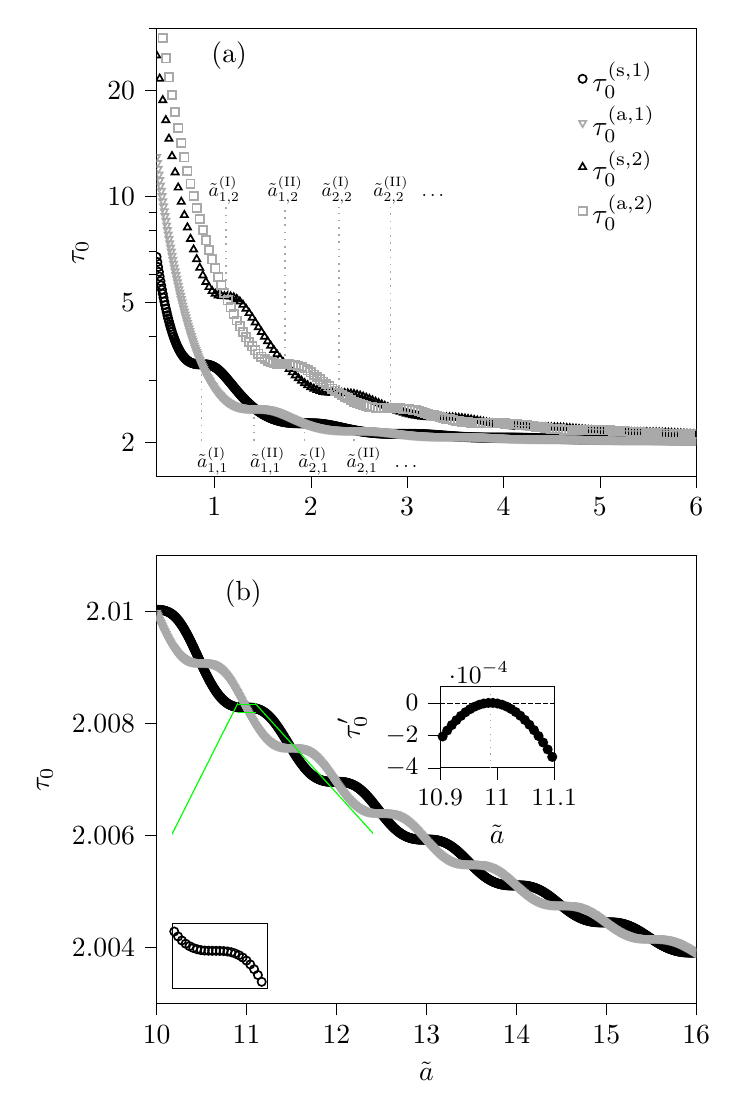
\begin{tikzpicture}

\definecolor{darkgray}{RGB}{169,169,169}
\definecolor{darkgray176}{RGB}{176,176,176}
\definecolor{lightgray204}{RGB}{204,204,204}

\begin{groupplot}[group style={group size=1 by 2},clip marker paths=true]
\nextgroupplot[
legend cell align={left},
legend style={fill opacity=0.8, draw opacity=1, text opacity=1, at={(0.95,0.95)}, draw=none},
log basis y={10},
tick align=outside,
tick pos=left,
x grid style={darkgray176},
xmin=0.4, xmax=6,
xtick style={color=black},
y grid style={darkgray176},
ylabel={\(\displaystyle \tau_0\)},
ymin=1.6, ymax=30,
ymode=log,
ytick style={color=black},
log ticks with fixed point, %afegit a ma
ytick={2,5,10,20}, %afegit a ma
minor ytick={3,4,6,7,8,9,30} %afegit a ma
]
\addplot [semithick, black, mark=o, mark size=1.5, mark options={solid,fill=none}, only marks]
table {%
0.4 6.72825292030247
0.408 6.50472697124453
0.416 6.29542811862217
0.424 6.09931777255341
0.432 5.91545229187631
0.44 5.74297269919318
0.448 5.5810956684581
0.456 5.42910560800124
0.464 5.28634768911461
0.472 5.15222169297914
0.48 5.02617656762402
0.488 4.9077056024444
0.496 4.7963421411059
0.504 4.69165576487054
0.512 4.59324888784717
0.52 4.50075371369173
0.528 4.41382951009721
0.536 4.3321601632177
0.544 4.25545197912645
0.552 4.1834317036493
0.56 4.11584473555358
0.568 4.05245351120064
0.576 3.99303604146579
0.584 3.9373845840565
0.592 3.88530443637343
0.6 3.83661283580419
0.608 3.79113795585573
0.616 3.7487179878511
0.624 3.70920029906621
0.632 3.67244065918824
0.64 3.63830252785762
0.648 3.6066563968287
0.656 3.57737918096583
0.664 3.55035365289329
0.672 3.52546791665344
0.68 3.50261491620545
0.688 3.48169197502918
0.696 3.46260036349192
0.704 3.44524489099944
0.712 3.42953352029495
0.72 3.41537700159799
0.728 3.40268852459844
0.736 3.39138338664719
0.744 3.38137867582299
0.752 3.37259296791516
0.76 3.36494603675231
0.768 3.35835857774024
0.776 3.35275194495659
0.784 3.34804790269751
0.792 3.34416839299049
0.8 3.34103532128661
0.808 3.33857036332753
0.816 3.33669479704719
0.824 3.33532936430497
0.832 3.33439416823546
0.84 3.33380861300257
0.848 3.33349139370581
0.856 3.33336054502354
0.864 3.33333355778063
0.872 3.33332757285928
0.88 3.33325966156223
0.888 3.33304720050134
0.896 3.33260834712624
0.904 3.33186261895565
0.912 3.33073157530565
0.92 3.32913959480441
0.928 3.32701473536321
0.936 3.32428965585236
0.944 3.32090257103383
0.952 3.31679820406723
0.96 3.31192869502812
0.968 3.30625442031033
0.976 3.29974467739081
0.984 3.29237819281517
0.992 3.28414341859159
1 3.27503859310346
1.008 3.26507155626806
1.016 3.25425932363295
1.024 3.24262743882019
1.032 3.2302091366228
1.04 3.21704435882346
1.048 3.2031786706164
1.056 3.18866212711595
1.064 3.1735481371314
1.072 3.15789236591412
1.08 3.14175171093658
1.088 3.12518337600966
1.096 3.10824406016065
1.104 3.09098926945622
1.112 3.07347275289031
1.12 3.05574605784447
1.128 3.03785819653573
1.136 3.01985541220195
1.144 3.00178103234679
1.152 2.98367539593512
1.16 2.96557584174608
1.168 2.9475167459249
1.176 2.92952959792775
1.184 2.91164310536922
1.192 2.8938833196401
1.2 2.87627377548193
1.208 2.85883563892912
1.216 2.84158785912984
1.224 2.82454732051988
1.232 2.80772899264669
1.24 2.79114607563233
1.248 2.7748101398335
1.256 2.7587312587189
1.264 2.74291813435254
1.272 2.72737821516095
1.28 2.7121178058846
1.288 2.69714216978188
1.296 2.6824556232774
1.304 2.6680616233339
1.312 2.65396284788661
1.32 2.64016126971595
1.328 2.62665822415478
1.336 2.61345447103349
1.344 2.60055025126384
1.352 2.58794533845299
1.36 2.57563908592478
1.368 2.56363046950755
1.376 2.55191812642822
1.384 2.54050039063116
1.392 2.52937532481947
1.4 2.51854074949484
1.408 2.50799426925167
1.416 2.49773329656125
1.424 2.48775507326301
1.432 2.47805668996156
1.44 2.46863510351212
1.448 2.45948715276071
1.456 2.45060957269139
1.464 2.44199900711916
1.472 2.43365202005491
1.48 2.42556510585734
1.488 2.41773469827627
1.496 2.41015717848238
1.504 2.40282888216949
1.512 2.39574610580747
1.52 2.38890511211673
1.528 2.38230213482839
1.536 2.37593338278834
1.544 2.36979504345765
1.552 2.36388328585707
1.56 2.35819426299837
1.568 2.35272411384167
1.576 2.34746896481348
1.584 2.34242493091744
1.592 2.33758811646606
1.6 2.33295461545946
1.608 2.32852051163428
1.616 2.32428187820386
1.624 2.32023477730878
1.632 2.316375259195
1.64 2.31269936113546
1.648 2.3092031061096
1.656 2.30588250125413
1.664 2.30273353609766
1.672 2.29975218059092
1.68 2.29693438294397
1.688 2.29427606728169
1.696 2.29177313112851
1.704 2.28942144273404
1.712 2.28721683825132
1.72 2.28515511878069
1.728 2.2832320472929
1.736 2.28144334544693
1.744 2.27978469031944
1.752 2.2782517110652
1.76 2.27683998553009
1.768 2.27554503684175
1.776 2.27436233000581
1.784 2.27328726854022
1.792 2.27231519118428
1.8 2.27144136872421
1.808 2.27066100098259
1.816 2.26996921402544
1.824 2.26936105764695
1.832 2.26883150319974
1.84 2.26837544184565
1.848 2.26798768331059
1.856 2.26766295523513
1.864 2.26739590322102
1.872 2.26718109168218
1.88 2.2670130056165
1.888 2.26688605342221
1.896 2.26679457088841
1.904 2.26673282649373
1.912 2.26669502814935
1.92 2.26667533152177
1.928 2.26666785006669
1.936 2.26666666689641
1.944 2.26666584859005
1.952 2.26665946103594
1.96 2.26664158737033
1.968 2.26660634804295
1.976 2.26654792300059
1.984 2.2664605759317
1.992 2.26633868046093
2 2.26617674812126
2.008 2.26596945786572
2.016 2.2657116868115
2.024 2.26539854183912
2.032 2.26502539160133
2.04 2.26458789843406
2.048 2.26408204960753
2.056 2.26350418731544
2.064 2.26285103677499
2.072 2.26211973180574
2.08 2.26130783727222
2.088 2.26041336781502
2.096 2.2594348023592
2.104 2.25837109397455
2.112 2.25722167476768
2.12 2.25598645560758
2.128 2.25466582061739
2.136 2.25326061650189
2.144 2.25177213691439
2.152 2.25020210219353
2.16 2.24855263491284
2.168 2.24682623178054
2.176 2.24502573249879
2.184 2.24315428623938
2.192 2.24121531641575
2.2 2.23921248442967
2.208 2.23714965304754
2.216 2.23503085001838
2.224 2.23286023248796
2.232 2.23064205269359
2.24 2.22838062534809
2.248 2.22608029704132
2.256 2.22374541790808
2.264 2.22138031573509
2.272 2.21898927260857
2.28 2.21657650414071
2.288 2.21414614125772
2.296 2.21170221448586
2.304 2.20924864063405
2.312 2.2067892117426
2.32 2.2043275861464
2.328 2.20186728148659
2.336 2.19941166949699
2.344 2.19696397238881
2.352 2.19452726065865
2.36 2.19210445215
2.368 2.18969831220607
2.376 2.18731145476106
2.384 2.18494634422811
2.392 2.18260529805346
2.4 2.18029048981812
2.408 2.17800395278039
2.416 2.17574758376365
2.424 2.17352314730533
2.432 2.17133227999277
2.44 2.16917649492177
2.448 2.16705718622216
2.456 2.16497563360305
2.464 2.16293300687746
2.472 2.16093037043278
2.48 2.15896868761904
2.488 2.15704882503243
2.496 2.15517155667565
2.504 2.1533375679808
2.512 2.15154745968379
2.52 2.14980175154224
2.528 2.1481008858912
2.536 2.14644523103319
2.544 2.1448350844609
2.552 2.14327067591218
2.56 2.14175217025838
2.568 2.14027967022796
2.576 2.1388532189681
2.584 2.13747280244788
2.592 2.1361383517068
2.6 2.13484974495311
2.608 2.13360680951658
2.616 2.13240932366048
2.624 2.131257018258
2.632 2.13014957833809
2.64 2.12908664450602
2.648 2.12806781424396
2.656 2.1270926430969
2.664 2.12616064574921
2.672 2.12527129699727
2.68 2.12442403262355
2.688 2.12361825017757
2.696 2.12285330966936
2.704 2.12212853418087
2.712 2.12144321040116
2.72 2.12079658909131
2.728 2.12018788548486
2.736 2.1196162796304
2.744 2.11908091668263
2.752 2.11858090714893
2.76 2.1181153270986
2.768 2.1176832183426
2.776 2.11728358859194
2.784 2.11691541160336
2.792 2.11657762732182
2.8 2.11626914202972
2.808 2.11598882851361
2.816 2.11573552625984
2.824 2.11550804169162
2.832 2.11530514846053
2.84 2.11512558780664
2.848 2.11496806900228
2.856 2.11483126989527
2.864 2.1147138375684
2.872 2.11461438913295
2.88 2.11453151267443
2.888 2.11446376836981
2.896 2.1144096897957
2.904 2.11436778544746
2.912 2.11433654048917
2.92 2.11431441875434
2.928 2.11429986501649
2.936 2.11429130754786
2.944 2.11428716098305
2.952 2.11428582950245
2.96 2.11428571034752
2.968 2.11428519767711
2.976 2.11428268676979
2.984 2.11427657857262
2.992 2.11426528459169
3 2.11424723211327
3.008 2.11422086973823
3.016 2.11418467320469
3.024 2.11413715146644
3.032 2.11407685298637
3.04 2.11400237219614
3.048 2.1139123560652
3.056 2.11380551071437
3.064 2.1136806080023
3.072 2.11353649200674
3.08 2.11337208531778
3.088 2.11318639505667
3.096 2.11297851853217
3.104 2.1127476484469
3.112 2.11249307756859
3.12 2.112214202786
3.128 2.11191052847653
3.136 2.11158166912153
3.144 2.11122735111703
3.152 2.1108474137403
3.16 2.11044180924731
3.168 2.11001060209129
3.176 2.10955396726847
3.184 2.1090721878128
3.192 2.10856565147652
3.2 2.10803484664758
3.208 2.10748035756744
3.216 2.10690285892357
3.224 2.10630310989955
3.232 2.10568194777181
3.24 2.10504028114617
3.248 2.10437908292852
3.256 2.10369938312351
3.264 2.10300226155194
3.272 2.10228884057304
3.28 2.10156027789147
3.288 2.10081775952146
3.296 2.10006249297207
3.304 2.09929570070852
3.312 2.09851861393579
3.32 2.09773246674086
3.328 2.09693849062161
3.336 2.09613790942179
3.344 2.09533193468344
3.352 2.09452176142137
3.36 2.09370856431782
3.368 2.09289349433
3.376 2.09207767569857
3.384 2.09126220334158
3.392 2.0904481406149
3.4 2.08963651741847
3.408 2.08882832862578
3.416 2.08802453281288
3.424 2.08722605126322
3.432 2.0864337672239
3.44 2.08564852538979
3.448 2.08487113159243
3.456 2.08410235267125
3.464 2.08334291650607
3.472 2.08259351219079
3.48 2.08185479032943
3.488 2.0811273634372
3.496 2.08041180643034
3.504 2.07970865719002
3.512 2.07901841718681
3.52 2.07834155215348
3.528 2.07767849279516
3.536 2.07702963552704
3.544 2.0763953432307
3.552 2.07577594602152
3.56 2.07517174202013
3.568 2.07458299812218
3.576 2.07400995076112
3.584 2.07345280665953
3.592 2.07291174356549
3.6 2.07238691097054
3.608 2.07187843080683
3.616 2.07138639812129
3.624 2.07091088172512
3.632 2.07045192481747
3.64 2.07000954558228
3.648 2.06958373775782
3.656 2.06917447117867
3.664 2.06878169229014
3.672 2.06840532463543
3.68 2.068045269316
3.688 2.06770140542596
3.696 2.06737359046127
3.704 2.0670616607051
3.712 2.06676543159039
3.72 2.06648469804133
3.728 2.06621923479534
3.736 2.06596879670739
3.744 2.06573311903879
3.752 2.06551191773254
3.76 2.06530488967781
3.768 2.06511171296598
3.776 2.06493204714123
3.784 2.06476553344853
3.792 2.06461179508238
3.8 2.06447043743968
3.808 2.06434104838045
3.816 2.06422319850022
3.824 2.06411644141838
3.832 2.06402031408667
3.84 2.06393433712261
3.848 2.06385801517253
3.856 2.06379083730936
3.864 2.06373227747032
3.872 2.06368179494003
3.88 2.06363883488448
3.888 2.06360282894161
3.896 2.06357319587416
3.904 2.06354934229056
3.912 2.06353066343949
3.92 2.06351654408356
3.928 2.0635063594575
3.936 2.0634994763157
3.944 2.06349525407358
3.952 2.06349304604669
3.96 2.06349220079073
3.968 2.06349206354477
3.976 2.06349197777898
3.984 2.06349128684684
3.992 2.06348933574087
4 2.06348547294887
4.008 2.06347905240652
4.016 2.06346943554007
4.024 2.06345599339123
4.032 2.06343810881427
4.04 2.06341517873328
4.048 2.06338661644569
4.056 2.06335185395594
4.064 2.06331034432156
4.072 2.06326156399179
4.08 2.06320501511775
4.088 2.06314022781145
4.096 2.06306676233024
4.104 2.06298421116264
4.112 2.06289220099112
4.12 2.06279039450801
4.128 2.06267849206109
4.136 2.06255623310714
4.144 2.06242339745298
4.152 2.06227980626628
4.16 2.0621253228407
4.168 2.06195985310331
4.176 2.06178334585555
4.184 2.0615957927425
4.192 2.06139722794947
4.2 2.06118772762824
4.208 2.06096740905965
4.216 2.06073642956263
4.224 2.06049498516323
4.232 2.06024330904064
4.24 2.05998166976947
4.248 2.05971036938043
4.256 2.05942974126279
4.264 2.05914014793373
4.272 2.05884197870027
4.28 2.05853564723963
4.288 2.05822158912386
4.296 2.05790025931359
4.304 2.057572129645
4.312 2.05723768633227
4.32 2.05689742750633
4.328 2.05655186080864
4.336 2.05620150105669
4.344 2.05584686799548
4.352 2.05548848414744
4.36 2.05512687277048
4.368 2.05476255593208
4.376 2.05439605270509
4.384 2.0540278774891
4.392 2.05365853845915
4.4 2.05328853614236
4.408 2.05291836212133
4.416 2.0525484978618
4.424 2.05217941366155
4.432 2.05181156771581
4.44 2.05144540529446
4.448 2.05108135802532
4.456 2.05071984327751
4.464 2.05036126363862
4.472 2.05000600647921
4.48 2.04965444359811
4.488 2.04930693094205
4.496 2.04896380839314
4.504 2.04862539961798
4.512 2.04829201197248
4.52 2.0479639364564
4.528 2.04764144771227
4.536 2.04732480406346
4.544 2.04701424758644
4.552 2.04671000421288
4.56 2.04641228385709
4.568 2.04612128056517
4.576 2.04583717268212
4.584 2.04556012303377
4.592 2.0452902791205
4.6 2.04502777332013
4.608 2.04477272309761
4.616 2.04452523121934
4.624 2.04428538597031
4.632 2.04405326137247
4.64 2.04382891740275
4.648 2.04361240020986
4.656 2.04340374232848
4.664 2.04320296289043
4.672 2.0430100678319
4.68 2.04282505009644
4.688 2.04264788983332
4.696 2.04247855459118
4.704 2.04231699950696
4.712 2.04216316749007
4.72 2.04201698940235
4.728 2.04187838423389
4.736 2.04174725927545
4.744 2.04162351028799
4.752 2.04150702166999
4.76 2.04139766662363
4.768 2.04129530732049
4.776 2.04119979506814
4.784 2.04111097047856
4.792 2.04102866363988
4.8 2.04095269429266
4.808 2.04088287201239
4.816 2.04081899639965
4.824 2.04076085727979
4.832 2.04070823491376
4.84 2.04066090022218
4.848 2.04061861502441
4.856 2.04058113229491
4.864 2.04054819643871
4.872 2.04051954358846
4.88 2.04049490192502
4.888 2.04047399202395
4.896 2.04045652723003
4.904 2.04044221406207
4.912 2.04043075265012
4.92 2.04042183720701
4.928 2.04041515653641
4.936 2.04041039457887
4.944 2.04040723099763
4.952 2.04040534180535
4.96 2.04040440003294
4.968 2.04040407644104
4.976 2.04040404027444
4.984 2.04040396005934
4.992 2.04040350444269
5 2.04040234307249
5.008 2.04040014751707
5.016 2.04039659222102
5.024 2.04039135549466
5.032 2.04038412053303
5.04 2.04037457646003
5.048 2.04036241939233
5.056 2.04034735351707
5.064 2.04032909217675
5.072 2.0403073589538
5.08 2.04028188874712
5.088 2.040252428832
5.096 2.0402187398947
5.104 2.04018059703242
5.112 2.04013779070949
5.12 2.04009012766023
5.128 2.04003743172946
5.136 2.03997954464149
5.144 2.03991632668933
5.152 2.03984765733592
5.16 2.03977343572051
5.168 2.03969358106389
5.176 2.03960803296716
5.184 2.03951675160037
5.192 2.03941971777795
5.2 2.03931693291978
5.208 2.03920841889778
5.216 2.0390942177693
5.224 2.03897439140015
5.232 2.03884902098117
5.24 2.03871820644361
5.248 2.03858206577966
5.256 2.0384407342755
5.264 2.03829436366504
5.272 2.03814312121328
5.28 2.0379871887386
5.288 2.0378267615839
5.296 2.03766204754635
5.304 2.03749326577583
5.312 2.03732064565185
5.32 2.03714442564844
5.328 2.03696485219615
5.336 2.03678217854974
5.344 2.0365966636696
5.352 2.03640857112409
5.36 2.03621816801938
5.368 2.03602572396267
5.376 2.03583151006354
5.384 2.03563579797794
5.392 2.03543885899791
5.4 2.03524096318993
5.408 2.03504237858372
5.416 2.03484337041282
5.424 2.03464420040763
5.432 2.03444512614092
5.44 2.03424640042555
5.448 2.03404827076341
5.456 2.03385097884448
5.464 2.03365476009437
5.472 2.03345984326853
5.48 2.03326645009117
5.488 2.03307479493657
5.496 2.03288508455053
5.504 2.03269751780955
5.512 2.03251228551527
5.52 2.03232957022162
5.528 2.03214954609246
5.536 2.03197237878701
5.544 2.03179822537093
5.552 2.03162723425072
5.56 2.03145954512915
5.568 2.03129528897987
5.576 2.03113458803892
5.584 2.03097755581158
5.592 2.03082429709258
5.6 2.03067490799822
5.608 2.0305294760088
5.616 2.03038808002002
5.624 2.03025079040209
5.632 2.03011766906543
5.64 2.02998876953189
5.648 2.02986413701064
5.656 2.02974380847788
5.664 2.02962781275969
5.672 2.02951617061745
5.68 2.02940889483526
5.688 2.0293059903091
5.696 2.0292074541372
5.704 2.0291132757117
5.712 2.02902343681108
5.72 2.02893791169373
5.728 2.02885666719226
5.736 2.02877966280903
5.744 2.02870685081277
5.752 2.02863817633674
5.76 2.02857357747862
5.768 2.02851298540262
5.776 2.02845632444412
5.784 2.02840351221749
5.792 2.02835445972761
5.8 2.0283090714857
5.808 2.02826724563016
5.816 2.02822887405322
5.824 2.02819384253411
5.832 2.0281620308797
5.84 2.02813331307334
5.848 2.02810755743306
5.856 2.02808462677981
5.864 2.028064378617
5.872 2.02804666532208
5.88 2.02803133435144
5.888 2.02801822845942
5.896 2.02800718593253
5.904 2.02799804083991
5.912 2.02799062330085
5.92 2.02798475977036
5.928 2.02798027334354
5.936 2.0279769840796
5.944 2.02797470934596
5.952 2.02797326418312
5.96 2.02797246169059
5.968 2.02797211343405
5.976 2.02797202987368
5.984 2.0279720208136
5.992 2.02797189587186
6 2.02797146497024
6.008 2.02797053884298
6.016 2.02796892956312
6.024 2.02796645108492
6.032 2.02796291980038
6.04 2.02795815510779
6.048 2.02795197998968
6.056 2.02794422159744
6.064 2.02793471183934
6.072 2.02792328796863
6.08 2.027909793168
6.088 2.02789407712641
6.096 2.02787599660432
6.104 2.02785541598285
6.112 2.02783220779275
6.12 2.02780625321849
6.128 2.0277774425734
6.136 2.02774567574127
6.144 2.02771086258049
6.152 2.02767292328665
6.16 2.02763178871012
6.168 2.02758740062518
6.176 2.02753971194796
6.184 2.02748868690075
6.192 2.02743430112087
6.2 2.02737654171264
6.208 2.02731540724198
6.216 2.02725090767324
6.224 2.02718306424896
6.232 2.02711190931352
6.24 2.02703748608243
6.248 2.02695984835945
6.256 2.02687906020427
6.264 2.026795195554
6.272 2.02670833780207
6.28 2.02661857933852
6.288 2.02652602105591
6.296 2.0264307718253
6.304 2.026332947947
6.312 2.02623267258056
6.32 2.0261300751589
6.328 2.02602529079099
6.336 2.02591845965772
6.344 2.02580972640512
6.352 2.02569923953913
6.36 2.02558715082571
6.368 2.02547361469977
6.376 2.02535878768617
6.384 2.02524282783569
6.392 2.02512589417843
6.4 2.02500814619693
6.408 2.02488974332063
6.416 2.02477084444351
6.424 2.02465160746567
6.432 2.02453218886013
6.44 2.02441274326503
6.448 2.02429342310186
6.456 2.02417437821957
6.464 2.02405575556448
6.472 2.02393769887566
6.48 2.02382034840512
6.488 2.02370384066236
6.496 2.02358830818224
6.504 2.02347387931541
6.512 2.02336067804031
6.52 2.02324882379569
6.528 2.02313843133243
6.536 2.02302961058385
6.544 2.02292246655303
6.552 2.02281709921627
6.56 2.0227136034415
6.568 2.02261206892045
6.576 2.02251258011369
6.584 2.02241521620737
6.592 2.02232005108074
6.6 2.0222271532835
6.608 2.02213658602208
6.616 2.022048407154
6.624 2.02196266918965
6.632 2.02187941930052
6.64 2.02179869933353
6.648 2.02172054583053
6.656 2.02164499005276
6.664 2.02157205800941
6.672 2.02150177049023
6.68 2.02143414310146
6.688 2.021369186305
6.696 2.02130690546047
6.704 2.02124730086995
6.712 2.02119036782516
6.72 2.02113609665711
6.728 2.0210844727881
6.736 2.02103547678593
6.744 2.02098908442056
6.752 2.02094526672312
6.76 2.02090399004751
6.768 2.02086521613464
6.776 2.02082890217957
6.784 2.02079500090185
6.792 2.02076346061916
6.8 2.02073422532476
6.808 2.02070723476896
6.816 2.02068242454508
6.824 2.02065972618016
6.832 2.02063906723109
6.84 2.02062037138639
6.848 2.02060355857418
6.856 2.02058854507698
6.864 2.02057524365359
6.872 2.02056356366881
6.88 2.02055341123127
6.888 2.02054468934018
6.896 2.02053729804118
6.904 2.02053113459199
6.912 2.02052609363829
6.92 2.02052206740017
6.928 2.02051894586954
6.936 2.02051661701901
6.944 2.02051496702223
6.952 2.02051388048611
6.96 2.02051324069494
6.968 2.02051292986645
6.976 2.02051282941968
6.984 2.02051282025462
6.992 2.02051278304307
7 2.02051259853043
7.008 2.0205121478478
7.016 2.02051131283357
7.024 2.02050997636365
7.032 2.02050802268926
7.04 2.02050533778108
7.048 2.02050180967824
7.056 2.02049732884082
7.064 2.02049178850393
7.072 2.02048508503165
7.08 2.02047711826876
7.088 2.02046779188828
7.096 2.02045701373246
7.104 2.02044469614501
7.112 2.02043075629227
7.12 2.02041511647091
7.128 2.02039770439975
7.136 2.02037845349349
7.144 2.020357303116
7.152 2.02033419881101
7.16 2.02030909250827
7.168 2.02028194270315
7.176 2.02025271460821
7.184 2.02022138027509
7.192 2.02018791868579
7.2 2.02015231581211
7.208 2.02011456464289
7.216 2.02007466517857
7.224 2.0200326243931
7.232 2.01998845616345
7.24 2.01994218116742
7.248 2.01989382675045
7.256 2.01984342676284
7.264 2.01979102136861
7.272 2.01973665682785
7.28 2.01968038525435
7.288 2.01962226435062
7.296 2.01956235712254
7.304 2.01950073157604
7.312 2.01943746039816
7.32 2.01937262062502
7.328 2.01930629329924
7.336 2.01923856311924
7.344 2.01916951808291
7.352 2.019099249128
7.36 2.01902784977152
7.368 2.01895541575025
7.376 2.0188820446645
7.384 2.01880783562684
7.392 2.01873288891762
7.4 2.01865730564873
7.408 2.01858118743703
7.416 2.01850463608857
7.424 2.01842775329461
7.432 2.01835064034037
7.44 2.01827339782701
7.448 2.0181961254075
7.456 2.01811892153662
7.464 2.01804188323545
7.472 2.01796510587027
7.48 2.01788868294602
7.488 2.01781270591398
7.496 2.01773726399371
7.504 2.01766244400871
7.512 2.01758833023555
7.52 2.01751500426602
7.528 2.01744254488176
7.536 2.01737102794101
7.544 2.01730052627667
7.552 2.01723110960542
7.56 2.01716284444708
7.568 2.0170957940537
7.576 2.01703001834786
7.584 2.01696557386952
7.592 2.01690251373092
7.6 2.01684088757894
7.608 2.01678074156441
7.616 2.01672211831787
7.624 2.01666505693129
7.632 2.01660959294533
7.64 2.01655575834162
7.648 2.01650358153984
7.656 2.01645308739906
7.664 2.01640429722307
7.672 2.0163572287695
7.68 2.01631189626232
7.688 2.01626831040754
7.696 2.01622647841195
7.704 2.01618640400469
7.712 2.01614808746151
7.72 2.01611152563164
7.728 2.01607671196716
7.736 2.01604363655487
7.744 2.01601228615058
7.752 2.01598264421592
7.76 2.01595469095765
7.768 2.01592840336946
7.776 2.0159037552766
7.784 2.01588071738317
7.792 2.01585925732235
7.8 2.0158393397098
7.808 2.01582092620028
7.816 2.0158039755477
7.824 2.01578844366899
7.832 2.0157742837118
7.84 2.01576144612642
7.848 2.01574987874221
7.856 2.01573952684862
7.864 2.01573033328133
7.872 2.01572223851361
7.88 2.01571518075322
7.888 2.01570909604519
7.896 2.01570391838061
7.904 2.01569957981191
7.912 2.01569601057456
7.92 2.01569313921568
7.928 2.01569089272963
7.936 2.0156891967007
7.944 2.01568797545308
7.952 2.01568715220819
7.96 2.0156866492493
7.968 2.0156863880935
7.976 2.01568628967094
7.984 2.01568627451101
7.992 2.01568626293545
8 2.0156861752579
8.008 2.01568593198954
8.016 2.01568545405041
8.024 2.0156846629857
8.032 2.01568348118646
8.04 2.0156818321139
8.048 2.01567964052648
8.056 2.01567683270879
8.064 2.01567333670128
8.072 2.01566908252963
8.08 2.01566400243267
8.088 2.01565803108755
8.096 2.01565110583085
8.104 2.01564316687435
8.112 2.01563415751398
8.12 2.01562402433066
8.128 2.01561271738151
8.136 2.0156001903802
8.144 2.01558640086498
8.152 2.01557131035314
8.16 2.01555488448069
8.168 2.01553709312606
8.176 2.01551791051693
8.184 2.01549731531911
8.192 2.01547529070679
8.2 2.01545182441358
8.208 2.01542690876374
8.216 2.0154005406834
8.224 2.01537272169164
8.232 2.0153434578714
8.24 2.01531275982055
8.248 2.01528064258336
8.256 2.01524712556314
8.264 2.01521223241655
8.272 2.01517599093059
8.28 2.01513843288323
8.288 2.01509959388878
8.296 2.01505951322925
8.304 2.015018233673
8.312 2.01497580128208
8.32 2.01493226520961
8.328 2.01488767748886
8.336 2.01484209281519
8.344 2.01479556832265
8.352 2.01474816335648
8.36 2.01469993924296
8.368 2.01465095905801
8.376 2.01460128739587
8.384 2.01455099013896
8.392 2.01450013423021
8.4 2.01444878744884
8.408 2.01439701819056
8.416 2.01434489525303
8.424 2.01429248762749
8.432 2.01423986429698
8.44 2.01418709404197
8.448 2.01413424525371
8.456 2.01408138575573
8.464 2.01402858263382
8.472 2.01397590207467
8.48 2.01392340921322
8.488 2.01387116798898
8.496 2.01381924101112
8.504 2.01376768943232
8.512 2.01371657283136
8.52 2.01366594910416
8.528 2.01361587436309
8.536 2.01356640284444
8.544 2.01351758682361
8.552 2.01346947653778
8.56 2.01342212011595
8.568 2.01337556351565
8.576 2.01332985046645
8.584 2.01328502241951
8.592 2.01324111850324
8.6 2.01319817548437
8.608 2.01315622773446
8.616 2.01311530720123
8.624 2.01307544338472
8.632 2.01303666331767
8.64 2.0129989915501
8.648 2.01296245013777
8.656 2.01292705863419
8.664 2.01289283408605
8.672 2.01285979103187
8.68 2.01282794150361
8.688 2.01279729503119
8.696 2.01276785864965
8.704 2.01273963690892
8.712 2.01271263188605
8.72 2.01268684319985
8.728 2.01266226802782
8.736 2.01263890112537
8.744 2.01261673484729
8.752 2.01259575917145
8.76 2.01257596172477
8.768 2.01255732781143
8.776 2.01253984044344
8.784 2.01252348037355
8.792 2.01250822613062
8.8 2.01249405405758
8.808 2.01248093835196
8.816 2.0124688511092
8.824 2.01245776236894
8.832 2.01244764016415
8.84 2.01243845057359
8.848 2.01243015777752
8.856 2.01242272411688
8.864 2.01241611015609
8.872 2.01241027474966
8.88 2.0124051751128
8.888 2.01240076689599
8.896 2.01239700426397
8.904 2.012393839979
8.912 2.01239122548867
8.92 2.01238911101837
8.928 2.01238744566846
8.936 2.01238617751618
8.944 2.01238525372251
8.952 2.01238462064375
8.96 2.01238422394804
8.968 2.01238400873663
8.976 2.01238391966978
8.984 2.01238390109735
8.992 2.01238389719363
9 2.01238385209638
9.008 2.01238371004973
9.016 2.01238341555062
9.024 2.01238291349835
9.032 2.0123821493468
9.04 2.01238106925895
9.048 2.01237962026291
9.056 2.01237775040907
9.064 2.01237540892756
9.072 2.01237254638536
9.08 2.01236911484236
9.088 2.01236506800547
9.096 2.01236036138001
9.104 2.01235495241756
9.112 2.01234880065926
9.12 2.01234186787392
9.128 2.01233411818972
9.136 2.01232551821901
9.144 2.012316037175
9.152 2.01230564697974
9.16 2.01229432236258
9.168 2.01228204094822
9.176 2.01226878333396
9.184 2.01225453315521
9.192 2.01223927713906
9.2 2.01222300514527
9.208 2.01220571019437
9.216 2.01218738848278
9.224 2.01216803938456
9.232 2.01214766544004
9.24 2.01212627233113
9.248 2.01210386884376
9.256 2.01208046681754
9.264 2.01205608108312
9.272 2.01203072938767
9.28 2.01200443230917
9.288 2.01197721316003
9.296 2.01194909788079
9.304 2.01192011492478
9.312 2.01189029513442
9.32 2.01185967161016
9.328 2.01182827957292
9.336 2.01179615622093
9.344 2.01176334058196
9.352 2.01172987336178
9.36 2.01169579678986
9.368 2.01166115446316
9.376 2.01162599118888
9.384 2.01159035282699
9.392 2.01155428613333
9.4 2.01151783860408
9.408 2.01148105832217
9.416 2.01144399380636
9.424 2.0114066938635
9.432 2.01136920744454
9.44 2.0113315835047
9.448 2.01129387086813
9.456 2.01125611809758
9.464 2.01121837336916
9.472 2.01118068435248
9.48 2.01114309809644
9.488 2.01110566092054
9.496 2.01106841831211
9.504 2.01103141482919
9.512 2.01099469400928
9.52 2.01095829828372
9.528 2.01092226889783
9.536 2.01088664583658
9.544 2.01085146775561
9.552 2.01081677191772
9.56 2.01078259413431
9.568 2.01074896871193
9.576 2.0107159284035
9.584 2.01068350436423
9.592 2.01065172611186
9.6 2.01062062149113
9.608 2.01059021664228
9.616 2.01056053597335
9.624 2.01053160213612
9.632 2.01050343600546
9.64 2.01047605666202
9.648 2.01044948137796
9.656 2.01042372560565
9.664 2.01039880296913
9.672 2.0103747252583
9.68 2.01035150242556
9.688 2.01032914258487
9.696 2.01030765201321
9.704 2.01028703515411
9.712 2.01026729462347
9.72 2.01024843121737
9.728 2.0102304439219
9.736 2.01021332992504
9.744 2.01019708463044
9.752 2.01018170167314
9.76 2.01016717293729
9.768 2.01015348857576
9.776 2.01014063703174
9.784 2.01012860506233
9.792 2.01011737776417
9.8 2.0101069386012
9.808 2.0100972694345
9.816 2.01008835055439
9.824 2.01008016071485
9.832 2.01007267717021
9.84 2.01006587571442
9.848 2.01005973072277
9.856 2.01005421519635
9.864 2.0100493008091
9.872 2.01004495795784
9.88 2.01004115581515
9.888 2.01003786238521
9.896 2.01003504456286
9.904 2.01003266819573
9.912 2.01003069814963
9.92 2.01002909837726
9.928 2.01002783199026
9.936 2.01002686133461
9.944 2.01002614806942
9.952 2.01002565324913
9.96 2.01002533740895
9.968 2.01002516065372
9.976 2.01002508274989
9.984 2.01002506322058
9.992 2.0100250614437
10 2.01002503675271
10.008 2.01002494854005
10.016 2.01002475636291
10.024 2.01002442005095
10.032 2.01002389981592
10.04 2.01002315636252
10.048 2.01002215100039
10.056 2.01002084575664
10.064 2.01001920348847
10.072 2.01001718799558
10.08 2.01001476413158
10.088 2.01001189791413
10.096 2.01000855663302
10.104 2.01000470895586
10.112 2.01000032503055
10.12 2.00999537658414
10.128 2.00998983701734
10.136 2.00998368149421
10.144 2.00997688702639
10.152 2.00996943255132
10.16 2.00996129900398
10.168 2.00995246938153
10.176 2.00994292880057
10.184 2.00993266454644
10.192 2.00992166611432
10.2 2.00990992524172
10.208 2.00989743593222
10.216 2.00988419447018
10.224 2.00987019942639
10.232 2.00985545165452
10.24 2.00983995427846
10.248 2.00982371267064
10.256 2.00980673442138
10.264 2.00978902929971
10.272 2.00977060920566
10.28 2.00975148811466
10.288 2.00973168201416
10.296 2.00971120883324
10.304 2.00969008836536
10.312 2.0096683421851
10.32 2.0096459935592
10.328 2.00962306735267
10.336 2.00959958993048
10.344 2.00957558905546
10.352 2.00955109378305
10.36 2.0095261343535
10.368 2.00950074208219
10.376 2.00947494924855
10.384 2.00944878898426
10.392 2.00942229516126
10.4 2.00939550228008
10.408 2.00936844535898
10.416 2.0093411598244
10.424 2.00931368140311
10.432 2.00928604601648
10.44 2.00925828967717
10.448 2.00923044838863
10.456 2.00920255804761
10.464 2.00917465434996
10.472 2.00914677269991
10.48 2.00911894812299
10.488 2.0090912151827
10.496 2.00906360790105
10.504 2.00903615968305
10.512 2.00900890324516
10.52 2.00898187054769
10.528 2.00895509273123
10.536 2.00892860005695
10.544 2.00890242185084
10.552 2.00887658645173
10.56 2.00885112116309
10.568 2.00882605220845
10.576 2.00880140469034
10.584 2.00877720255274
10.592 2.00875346854678
10.6 2.00873022419965
10.608 2.00870748978663
10.616 2.00868528430605
10.624 2.0086636254571
10.632 2.00864252962028
10.64 2.00862201184063
10.648 2.00860208581324
10.656 2.00858276387128
10.664 2.00856405697627
10.672 2.00854597471052
10.68 2.00852852527168
10.688 2.00851171546931
10.696 2.00849555072338
10.704 2.00848003506465
10.712 2.00846517113686
10.72 2.00845096020072
10.728 2.00843740213957
10.736 2.0084244954668
10.744 2.00841223733492
10.752 2.00840062354627
10.76 2.0083896485654
10.768 2.00837930553309
10.776 2.00836958628204
10.784 2.00836048135423
10.792 2.00835198001999
10.8 2.00834407029878
10.808 2.0083367389817
10.816 2.00832997165591
10.824 2.00832375273077
10.832 2.00831806546594
10.84 2.00831289200144
10.848 2.00830821338966
10.856 2.00830400962952
10.864 2.00830025970261
10.872 2.00829694161166
10.88 2.00829403242112
10.888 2.00829150830006
10.896 2.00828934456741
10.904 2.00828751573958
10.912 2.00828599558044
10.92 2.00828475715379
10.928 2.00828377287825
10.936 2.00828301458462
10.944 2.00828245357574
10.952 2.00828206068867
10.96 2.00828180635942
10.968 2.00828166068994
10.976 2.00828159351739
10.984 2.00828157448563
10.992 2.00828157311878
11 2.00828155889672
11.008 2.00828150133237
11.016 2.00828137005057
11.024 2.0082811348684
11.032 2.00828076587665
11.04 2.00828023352216
11.048 2.00827950869093
11.056 2.00827856279145
11.064 2.00827736783811
11.072 2.00827589653431
11.08 2.00827412235485
11.088 2.00827201962726
11.096 2.00826956361176
11.104 2.00826673057928
11.112 2.00826349788725
11.12 2.00825984405278
11.128 2.00825574882269
11.136 2.00825119324006
11.144 2.00824615970693
11.152 2.00824063204269
11.16 2.00823459553783
11.168 2.00822803700271
11.176 2.008220944811
11.184 2.00821330893749
11.192 2.00820512099007
11.2 2.00819637423561
11.208 2.00818706361952
11.216 2.00817718577892
11.224 2.00816673904935
11.232 2.00815572346482
11.24 2.00814414075136
11.248 2.00813199431403
11.256 2.00811928921748
11.264 2.00810603216025
11.272 2.0080922314429
11.28 2.00807789693026
11.288 2.00806304000809
11.296 2.0080476735343
11.304 2.00803181178521
11.312 2.00801547039717
11.32 2.00799866630383
11.328 2.00798141766958
11.336 2.00796374381949
11.344 2.00794566516622
11.352 2.00792720313428
11.36 2.0079083800822
11.368 2.00788921922281
11.376 2.0078697445423
11.384 2.00784998071833
11.392 2.00782995303763
11.4 2.00780968731345
11.408 2.00778920980329
11.416 2.00776854712717
11.424 2.00774772618684
11.432 2.00772677408617
11.44 2.00770571805305
11.448 2.00768458536295
11.456 2.00766340326451
11.464 2.00764219890719
11.472 2.00762099927132
11.48 2.00759983110051
11.488 2.00757872083671
11.496 2.00755769455791
11.504 2.0075367779186
11.512 2.00751599609305
11.52 2.00749537372135
11.528 2.00747493485844
11.536 2.00745470292586
11.544 2.00743470066646
11.552 2.00741495010184
11.56 2.0073954724926
11.568 2.00737628830136
11.576 2.00735741715839
11.584 2.0073388778299
11.592 2.00732068818886
11.6 2.00730286518828
11.608 2.00728542483693
11.616 2.00726838217729
11.624 2.00725175126584
11.632 2.00723554515545
11.64 2.00721977587987
11.648 2.00720445444019
11.656 2.00718959079333
11.664 2.00717519384227
11.672 2.0071612714282
11.68 2.00714783032428
11.688 2.00713487623117
11.696 2.00712241377417
11.704 2.00711044650188
11.712 2.00709897688648
11.72 2.00708800632541
11.728 2.00707753514462
11.736 2.00706756260318
11.744 2.00705808689933
11.752 2.00704910517798
11.76 2.00704061353957
11.768 2.0070326070503
11.776 2.00702507975385
11.784 2.00701802468441
11.792 2.00701143388118
11.8 2.00700529840431
11.808 2.00699960835226
11.816 2.00699435288068
11.824 2.00698952022278
11.832 2.00698509771124
11.84 2.00698107180169
11.848 2.0069774280978
11.856 2.00697415137802
11.864 2.00697122562397
11.872 2.00696863405055
11.88 2.00696635913784
11.888 2.00696438266465
11.896 2.00696268574404
11.904 2.00696124886051
11.912 2.0069600519091
11.92 2.00695907423638
11.928 2.0069582946832
11.936 2.00695769162938
11.944 2.00695724304021
11.952 2.00695692651475
11.96 2.00695671933594
11.968 2.00695659852242
11.976 2.00695654088207
11.984 2.00695652306707
11.992 2.00695652163057
12 2.00695651308468
12.008 2.00695647395977
12.016 2.00695638086496
12.024 2.00695621054952
12.032 2.00695593996515
12.04 2.00695554632886
12.048 2.00695500718626
12.056 2.00695430047511
12.064 2.00695340458874
12.072 2.00695229843927
12.08 2.00695096152025
12.088 2.00694937396843
12.096 2.0069475166245
12.104 2.00694537109239
12.112 2.00694291979685
12.12 2.00694014603909
12.128 2.00693703405008
12.136 2.0069335690413
12.144 2.00692973725259
12.152 2.00692552599685
12.16 2.0069209237013
12.168 2.00691591994511
12.176 2.00691050549308
12.184 2.00690467232515
12.192 2.0068984136617
12.2 2.00689172398427
12.208 2.00688459905167
12.216 2.00687703591144
12.224 2.00686903290636
12.232 2.00686058967622
12.24 2.00685170715471
12.248 2.00684238756137
12.256 2.00683263438887
12.264 2.00682245238549
12.272 2.00681184753305
12.28 2.00680082702037
12.288 2.0067893992125
12.296 2.0067775736158
12.304 2.00676536083927
12.312 2.00675277255222
12.32 2.00673982143859
12.328 2.00672652114831
12.336 2.00671288624576
12.344 2.00669893215587
12.352 2.00668467510806
12.36 2.00667013207828
12.368 2.0066553207296
12.376 2.0066402593515
12.384 2.00662496679829
12.392 2.00660946242694
12.4 2.00659376603453
12.408 2.00657789779563
12.416 2.00656187819998
12.424 2.00654572799048
12.432 2.00652946810204
12.44 2.00651311960116
12.448 2.00649670362672
12.456 2.00648024133201
12.464 2.00646375382817
12.472 2.00644726212925
12.48 2.00643078709894
12.488 2.00641434939911
12.496 2.0063979694403
12.504 2.00638166733408
12.512 2.00636546284754
12.52 2.00634937535978
12.528 2.00633342382058
12.536 2.00631762671109
12.544 2.00630200200672
12.552 2.00628656714214
12.56 2.00627133897838
12.568 2.00625633377197
12.576 2.00624156714625
12.584 2.00622705406456
12.592 2.00621280880552
12.6 2.00619884494021
12.608 2.00618517531121
12.616 2.00617181201353
12.624 2.00615876637728
12.632 2.00614604895212
12.64 2.00613366949334
12.648 2.00612163694966
12.656 2.00610995945246
12.664 2.00609864430674
12.672 2.00608769798337
12.68 2.00607712611293
12.688 2.00606693348086
12.696 2.006057124024
12.704 2.00604770082848
12.712 2.00603866612886
12.72 2.00603002130856
12.728 2.00602176690153
12.736 2.00601390259516
12.744 2.00600642723436
12.752 2.00599933882689
12.76 2.00599263454981
12.768 2.00598631075719
12.776 2.00598036298894
12.784 2.00597478598086
12.792 2.00596957367586
12.8 2.00596471923643
12.808 2.00596021505828
12.816 2.00595605278521
12.824 2.00595222332526
12.832 2.0059487168681
12.84 2.00594552290371
12.848 2.00594263024238
12.856 2.00594002703605
12.864 2.00593770080091
12.872 2.00593563844155
12.88 2.00593382627628
12.888 2.00593225006405
12.896 2.00593089503268
12.904 2.00592974590856
12.912 2.00592878694779
12.92 2.00592800196874
12.928 2.0059273743861
12.936 2.00592688724632
12.944 2.00592652326447
12.952 2.00592626486248
12.96 2.00592609420881
12.968 2.00592599325932
12.976 2.0059259437995
12.984 2.00592592748785
12.992 2.00592592590042
13 2.00592592057637
13.008 2.00592589306449
13.016 2.00592582497055
13.024 2.00592569800538
13.032 2.00592549403353
13.04 2.00592519512235
13.048 2.00592478359139
13.056 2.00592424206189
13.064 2.00592355350617
13.072 2.00592270129687
13.08 2.0059216692556
13.088 2.00592044170106
13.096 2.00591900349618
13.104 2.00591734009425
13.112 2.00591543758371
13.12 2.00591328273139
13.128 2.00591086302404
13.136 2.00590816670786
13.144 2.00590518282584
13.152 2.00590190125269
13.16 2.00589831272724
13.168 2.00589440888198
13.176 2.00589018226965
13.184 2.00588562638676
13.192 2.00588073569377
13.2 2.00587550563195
13.208 2.00586993263668
13.216 2.00586401414719
13.224 2.00585774861265
13.232 2.00585113549458
13.24 2.00584417526555
13.248 2.00583686940419
13.256 2.00582922038655
13.264 2.00582123167378
13.272 2.00581290769644
13.28 2.00580425383518
13.288 2.00579527639831
13.296 2.00578598259606
13.304 2.00577638051191
13.312 2.00576647907109
13.32 2.00575628800643
13.328 2.00574581782173
13.336 2.00573507975301
13.344 2.00572408572769
13.352 2.00571284832197
13.36 2.00570138071674
13.368 2.00568969665213
13.376 2.00567781038099
13.384 2.00566573662151
13.392 2.00565349050924
13.4 2.00564108754864
13.408 2.00562854356453
13.416 2.00561587465344
13.424 2.00560309713523
13.432 2.00559022750503
13.44 2.00557728238583
13.448 2.00556427848162
13.456 2.00555123253152
13.464 2.00553816126484
13.472 2.0055250813572
13.48 2.00551200938794
13.488 2.00549896179874
13.496 2.00548595485367
13.504 2.0054730046007
13.512 2.00546012683465
13.52 2.00544733706172
13.528 2.00543465046563
13.536 2.00542208187531
13.544 2.00540964573421
13.552 2.00539735607132
13.56 2.0053852264737
13.568 2.00537327006071
13.576 2.00536149945982
13.584 2.00534992678398
13.592 2.00533856361064
13.6 2.00532742096218
13.608 2.00531650928798
13.616 2.00530583844788
13.624 2.00529541769712
13.632 2.00528525567266
13.64 2.00527536038092
13.648 2.00526573918681
13.656 2.0052563988041
13.664 2.00524734528704
13.672 2.00523858402319
13.68 2.00523011972753
13.688 2.00522195643765
13.696 2.00521409751016
13.704 2.00520654561816
13.712 2.00519930274988
13.72 2.0051923702083
13.728 2.00518574861191
13.736 2.00517943789647
13.744 2.00517343731782
13.752 2.00516774545569
13.76 2.00516236021854
13.768 2.00515727884938
13.776 2.00515249793265
13.784 2.00514801340204
13.792 2.0051438205494
13.8 2.00513991403455
13.808 2.00513628789626
13.816 2.00513293556412
13.824 2.00512984987155
13.832 2.00512702306985
13.84 2.00512444684323
13.848 2.00512211232506
13.856 2.00512001011508
13.864 2.00511813029782
13.872 2.00511646246207
13.88 2.00511499572147
13.888 2.00511371873633
13.896 2.00511261973648
13.904 2.00511168654533
13.912 2.00511090660508
13.92 2.00511026700307
13.928 2.00510975449925
13.936 2.0051093555548
13.944 2.00510905636185
13.952 2.00510884287433
13.96 2.00510870083978
13.968 2.0051086158323
13.976 2.00510857328637
13.984 2.0051085585317
13.992 2.00510855682881
14 2.00510855340555
14.008 2.00510853349422
14.016 2.00510848236941
14.024 2.00510838538628
14.032 2.00510822801934
14.04 2.00510799590153
14.048 2.00510767486349
14.056 2.00510725097284
14.064 2.00510671057346
14.072 2.00510604032451
14.08 2.00510522723906
14.088 2.00510425872218
14.096 2.00510312260839
14.104 2.00510180719816
14.112 2.00510030129345
14.12 2.005098594232
14.128 2.00509667592027
14.136 2.00509453686483
14.144 2.00509216820205
14.152 2.00508956172593
14.16 2.00508670991394
14.168 2.00508360595061
14.176 2.00508024374896
14.184 2.00507661796939
14.192 2.00507272403612
14.2 2.00506855815097
14.208 2.00506411730443
14.216 2.00505939928395
14.224 2.00505440267942
14.232 2.00504912688579
14.24 2.00504357210274
14.248 2.00503773933161
14.256 2.00503163036935
14.264 2.00502524779971
14.272 2.00501859498163
14.28 2.005011676035
14.288 2.00500449582378
14.296 2.00499705993657
14.304 2.00498937466487
14.312 2.00498144697907
14.32 2.00497328450227
14.328 2.0049648954822
14.336 2.0049562887613
14.344 2.00494747374516
14.352 2.0049384603695
14.36 2.00492925906585
14.368 2.00491988072608
14.376 2.00491033666605
14.384 2.00490063858842
14.392 2.00489079854493
14.4 2.0048808288982
14.408 2.00487074228327
14.416 2.00486055156912
14.424 2.00485026982011
14.432 2.00483991025772
14.44 2.00482948622258
14.448 2.00481901113693
14.456 2.00480849846769
14.464 2.00479796169024
14.472 2.00478741425287
14.48 2.00477686954227
14.488 2.00476634084979
14.496 2.00475584133885
14.504 2.00474538401336
14.512 2.00473498168734
14.52 2.00472464695561
14.528 2.00471439216577
14.536 2.00470422939142
14.544 2.00469417040658
14.552 2.00468422666138
14.56 2.00467440925913
14.568 2.00466472893451
14.576 2.00465519603313
14.584 2.00464582049238
14.592 2.00463661182344
14.6 2.00462757909458
14.608 2.00461873091571
14.616 2.00461007542407
14.624 2.00460162027114
14.632 2.0045933726107
14.64 2.00458533908799
14.648 2.00457752583004
14.656 2.004569938437
14.664 2.00456258197463
14.672 2.0045554609677
14.68 2.00454857939455
14.688 2.00454194068248
14.696 2.00453554770427
14.704 2.0045294027755
14.712 2.00452350765292
14.72 2.00451786353368
14.728 2.00451247105545
14.736 2.00450733029751
14.744 2.0045024407826
14.752 2.00449780147976
14.76 2.00449341080797
14.768 2.00448926664066
14.776 2.00448536631112
14.784 2.00448170661868
14.792 2.0044782838359
14.8 2.00447509371645
14.808 2.00447213150398
14.816 2.00446939194184
14.824 2.00446686928364
14.832 2.00446455730471
14.84 2.00446244931451
14.848 2.00446053816986
14.856 2.00445881628911
14.864 2.00445727566726
14.872 2.00445590789197
14.88 2.00445470416048
14.888 2.00445365529749
14.896 2.00445275177401
14.904 2.00445198372708
14.912 2.00445134098042
14.92 2.0044508130661
14.928 2.00445038924702
14.936 2.00445005854037
14.944 2.00444980974192
14.952 2.00444963145122
14.96 2.00444951209765
14.968 2.0044494399672
14.976 2.00444940323013
14.984 2.00444938996926
14.992 2.00444938820897
15 2.00444938594484
15.008 2.0044493711738
15.016 2.00444933192478
15.024 2.0044492562898
15.032 2.0044491324553
15.04 2.00444894873378
15.048 2.00444869359553
15.056 2.00444835570037
15.064 2.00444792392937
15.072 2.00444738741629
15.08 2.00444673557877
15.088 2.00444595814907
15.096 2.00444504520416
15.104 2.00444398719526
15.112 2.00444277497637
15.12 2.00444139983202
15.128 2.00443985350376
15.136 2.00443812821553
15.144 2.00443621669768
15.152 2.00443411220941
15.16 2.00443180855975
15.168 2.00442930012671
15.176 2.00442658187473
15.184 2.00442364937013
15.192 2.0044204987946
15.2 2.00441712695664
15.208 2.00441353130079
15.216 2.00440970991475
15.224 2.00440566153418
15.232 2.00440138554532
15.24 2.00439688198527
15.248 2.00439215154001
15.256 2.00438719554014
15.264 2.0043820159544
15.272 2.00437661538099
15.28 2.0043709970367
15.288 2.00436516474399
15.296 2.00435912291605
15.304 2.00435287653992
15.312 2.00434643115782
15.32 2.00433979284673
15.328 2.00433296819637
15.336 2.0043259642857
15.344 2.00431878865807
15.352 2.00431144929509
15.36 2.00430395458953
15.368 2.00429631331709
15.376 2.00428853460749
15.384 2.00428062791484
15.392 2.0042726029874
15.4 2.00426446983706
15.408 2.00425623870834
15.416 2.00424792004747
15.424 2.00423952447122
15.432 2.00423106273596
15.44 2.00422254570682
15.448 2.00421398432719
15.456 2.00420538958863
15.464 2.00419677250116
15.472 2.00418814406428
15.48 2.00417951523844
15.488 2.0041708969174
15.496 2.0041622999012
15.504 2.00415373487006
15.512 2.00414521235908
15.52 2.00413674273389
15.528 2.00412833616725
15.536 2.00412000261652
15.544 2.00411175180224
15.552 2.00410359318765
15.56 2.00409553595923
15.568 2.00408758900828
15.576 2.00407976091346
15.584 2.00407205992449
15.592 2.00406449394667
15.6 2.0040570705266
15.608 2.00404979683877
15.616 2.00404267967321
15.624 2.00403572542404
15.632 2.00402894007907
15.64 2.00402232921025
15.648 2.00401589796513
15.656 2.00400965105915
15.664 2.00400359276886
15.672 2.00399772692605
15.68 2.00399205691263
15.688 2.00398658565646
15.696 2.00398131562797
15.704 2.00397624883755
15.712 2.00397138683378
15.72 2.00396673070249
15.728 2.00396228106646
15.736 2.00395803808603
15.744 2.00395400146039
15.752 2.00395017042965
15.76 2.00394654377763
15.768 2.00394311983542
15.776 2.00393989648565
15.784 2.00393687116754
15.792 2.00393404088269
15.8 2.0039314022015
15.808 2.00392895127052
15.816 2.00392668382037
15.824 2.0039245951745
15.832 2.00392268025871
15.84 2.00392093361137
15.848 2.00391934939443
15.856 2.0039179214052
15.864 2.00391664308892
15.872 2.00391550755202
15.88 2.00391450757627
15.888 2.0039136356336
15.896 2.00391288390176
15.904 2.00391224428076
15.912 2.00391170840997
15.92 2.00391126768614
15.928 2.00391091328207
15.936 2.00391063616602
15.944 2.00391042712187
15.952 2.00391027676998
15.96 2.00391017558872
15.968 2.00391011393662
15.976 2.00391008207521
15.984 2.00391007019237
15.992 2.00391006842622
16 2.00391006688955
16.008 2.00391005569462
16.016 2.00391002497838
16.024 2.00390996492799
16.032 2.00390986580658
16.04 2.00390971797916
16.048 2.00390951193866
16.056 2.00390923833197
16.064 2.00390888798586
16.072 2.00390845193274
16.08 2.0039079214362
16.088 2.0039072880161
16.096 2.00390654347328
16.104 2.00390567991356
16.112 2.00390468977124
16.12 2.00390356583168
16.128 2.00390230125302
16.136 2.00390088958694
16.144 2.00389932479832
16.152 2.00389760128369
16.16 2.00389571388842
16.168 2.0038936579225
16.176 2.0038914291749
16.184 2.00388902392638
16.192 2.0038864389607
16.2 2.00388367157417
16.208 2.00388071958344
16.216 2.00387758133161
16.224 2.00387425569246
16.232 2.00387074207289
16.24 2.00386704041355
16.248 2.00386315118759
16.256 2.00385907539764
16.264 2.00385481457088
16.272 2.00385037075244
16.28 2.00384574649699
16.288 2.00384094485861
16.296 2.00383596937913
16.304 2.00383082407476
16.312 2.00382551342137
16.32 2.00382004233818
16.328 2.0038144161703
16.336 2.00380864066993
16.344 2.00380272197645
16.352 2.00379666659546
16.36 2.00379048137697
16.368 2.00378417349266
16.376 2.0037777504125
16.384 2.00377121988076
16.392 2.00376458989152
16.4 2.00375786866375
16.408 2.0037510646162
16.416 2.00374418634201
16.424 2.0037372425833
16.432 2.00373024220577
16.44 2.00372319417334
16.448 2.00371610752308
16.456 2.00370899134031
16.464 2.0037018547341
16.472 2.00369470681318
16.48 2.00368755666228
16.488 2.00368041331907
16.496 2.00367328575163
16.504 2.00366618283659
16.512 2.00365911333792
16.52 2.00365208588647
16.528 2.00364510896018
16.536 2.00363819086513
16.544 2.00363133971733
16.552 2.00362456342536
16.56 2.00361786967375
16.568 2.0036112659073
16.576 2.00360475931613
16.584 2.00359835682159
16.592 2.00359206506306
16.6 2.0035858903855
16.608 2.00357983882789
16.616 2.00357391611244
16.624 2.00356812763466
16.632 2.00356247845416
16.64 2.00355697328635
16.648 2.00355161649479
16.656 2.00354641208442
16.664 2.00354136369546
16.672 2.0035364745981
16.68 2.00353174768792
16.688 2.00352718548199
16.696 2.00352279011575
16.704 2.00351856334049
16.712 2.0035145065216
16.72 2.00351062063747
16.728 2.00350690627904
16.736 2.00350336365003
16.744 2.00349999256784
16.752 2.00349679246507
16.76 2.0034937623917
16.768 2.00349090101792
16.776 2.00348820663759
16.784 2.00348567717235
16.792 2.00348331017633
16.8 2.00348110284157
16.808 2.003479052004
16.816 2.00347715415012
16.824 2.00347540542428
16.832 2.00347380163662
16.84 2.0034723382717
16.848 2.00347101049766
16.856 2.00346981317616
16.864 2.00346874087291
16.872 2.00346778786884
16.88 2.00346694817197
16.888 2.00346621552986
16.896 2.0034655834428
16.904 2.00346504517757
16.912 2.00346459378185
16.92 2.00346422209933
16.928 2.00346392278535
16.936 2.00346368832319
16.944 2.00346351104099
16.952 2.00346338312915
16.96 2.0034632966584
16.968 2.00346324359834
16.976 2.00346321583642
16.984 2.00346320519754
16.992 2.00346320346393
17 2.0034632023955
17.008 2.00346319375055
17.016 2.00346316930671
17.024 2.00346312088218
17.032 2.00346304035715
17.04 2.00346291969531
17.048 2.0034627509655
17.056 2.00346252636326
17.064 2.00346223823234
17.072 2.00346187908613
17.08 2.0034614416287
17.088 2.00346091877567
17.096 2.00346030367463
17.104 2.00345958972508
17.112 2.0034587705978
17.12 2.0034578402536
17.128 2.00345679296134
17.136 2.0034556233151
17.144 2.00345432625049
17.152 2.00345289705998
17.16 2.00345133140717
17.168 2.00344962533993
17.176 2.00344777530238
17.184 2.00344577814562
17.192 2.00344363113712
17.2 2.00344133196876
17.208 2.00343887876349
17.216 2.00343627008055
17.224 2.00343350491924
17.232 2.00343058272111
17.24 2.0034275033708
17.248 2.00342426719527
17.256 2.00342087496157
17.264 2.00341732787314
17.272 2.00341362756461
17.28 2.0034097760952
17.288 2.00340577594073
17.296 2.00340162998423
17.304 2.00339734150533
17.312 2.0033929141683
17.32 2.00338835200906
17.328 2.00338365942093
17.336 2.00337884113942
17.344 2.00337390222612
17.352 2.0033688480516
17.36 2.00336368427757
17.368 2.00335841683838
17.376 2.00335305192184
17.384 2.00334759594953
17.392 2.00334205555669
17.4 2.00333643757169
17.408 2.00333074899533
17.416 2.00332499697984
17.424 2.00331918880785
17.432 2.00331333187132
17.44 2.00330743365046
17.448 2.00330150169286
17.456 2.00329554359268
17.464 2.00328956697025
17.472 2.00328357945177
17.48 2.00327758864958
17.488 2.00327160214266
17.496 2.00326562745771
17.504 2.00325967205068
17.512 2.00325374328879
17.52 2.00324784843318
17.528 2.00324199462214
17.536 2.00323618885491
17.544 2.00323043797616
17.552 2.00322474866114
17.56 2.00321912740143
17.568 2.00321358049142
17.576 2.00320811401546
17.584 2.00320273383573
17.592 2.00319744558071
17.6 2.00319225463444
17.608 2.00318716612645
17.616 2.00318218492231
17.624 2.00317731561493
17.632 2.00317256251655
17.64 2.00316792965131
17.648 2.00316342074856
17.656 2.0031590392368
17.664 2.00315478823828
17.672 2.00315067056415
17.68 2.00314668871041
17.688 2.00314284485428
17.696 2.00313914085132
17.704 2.00313557823312
17.712 2.00313215820554
17.72 2.00312888164755
17.728 2.00312574911075
17.736 2.0031227608193
17.744 2.00311991667054
17.752 2.00311721623615
17.76 2.00311465876385
17.768 2.00311224317968
17.776 2.0031099680908
17.784 2.00310783178893
17.792 2.00310583225423
17.8 2.00310396715983
17.808 2.00310223387685
17.816 2.00310062948003
17.824 2.00309915075382
17.832 2.00309779419918
17.84 2.00309655604077
17.848 2.00309543223478
17.856 2.00309441847734
17.864 2.00309351021344
17.872 2.0030927026464
17.88 2.00309199074795
17.888 2.00309136926878
17.896 2.00309083274975
17.904 2.00309037553353
17.912 2.00308999177687
17.92 2.00308967546333
17.928 2.00308942041659
17.936 2.00308922031424
17.944 2.00308906870202
17.952 2.00308895900868
17.96 2.00308888456112
17.968 2.00308883860008
17.976 2.00308881429623
17.984 2.00308880476661
17.992 2.00308880309145
18 2.0030888023313
18.008 2.00308879554444
18.016 2.0030887758045
18.024 2.00308873621836
18.032 2.00308866994408
18.04 2.00308857020905
18.048 2.00308843032806
18.056 2.00308824372144
18.064 2.00308800393312
18.072 2.0030877046485
18.08 2.00308733971218
18.088 2.00308690314537
18.096 2.00308638916303
18.104 2.00308579219056
18.112 2.00308510688002
18.12 2.00308432812582
18.128 2.00308345107984
18.136 2.00308247116579
18.144 2.00308138409291
18.152 2.00308018586882
18.16 2.0030788728115
18.168 2.00307744156038
18.176 2.00307588908638
18.184 2.003074212701
18.192 2.00307241006425
18.2 2.00307047919154
18.208 2.00306841845934
18.216 2.0030662266097
18.224 2.00306390275356
18.232 2.00306144637278
18.24 2.00305885732103
18.248 2.00305613582333
18.256 2.00305328247442
18.264 2.00305029823591
18.272 2.00304718443212
18.28 2.00304394274489
18.288 2.00304057520708
18.296 2.00303708419498
18.304 2.00303347241973
18.312 2.00302974291756
18.32 2.00302589903914
18.328 2.00302194443796
18.336 2.00301788305783
18.344 2.00301371911957
18.352 2.003009457107
18.36 2.00300510175219
18.368 2.0030006580201
18.376 2.00299613109278
18.384 2.00299152635294
18.392 2.0029868493673
18.4 2.00298210586946
18.408 2.00297730174265
18.416 2.00297244300217
18.424 2.00296753577782
18.432 2.0029625862962
18.44 2.00295760086304
18.448 2.00295258584563
18.456 2.00294754765531
18.464 2.00294249273021
18.472 2.00293742751813
18.48 2.00293235845979
18.488 2.00292729197235
18.496 2.00292223443322
18.504 2.00291719216443
18.512 2.00291217141725
18.52 2.00290717835734
18.528 2.00290221905042
18.536 2.00289729944834
18.544 2.00289242537579
18.552 2.00288760251742
18.56 2.0028828364056
18.568 2.00287813240873
18.576 2.00287349572005
18.584 2.00286893134715
18.592 2.0028644441019
18.6 2.00286003859112
18.608 2.0028557192077
18.616 2.00285149012238
18.624 2.0028473552761
18.632 2.00284331837287
18.64 2.00283938287326
18.648 2.00283555198848
18.656 2.00283182867494
18.664 2.00282821562941
18.672 2.00282471528476
18.68 2.00282132980619
18.688 2.00281806108798
18.696 2.00281491075088
18.704 2.00281188013985
18.712 2.00280897032249
18.72 2.00280618208786
18.728 2.00280351594589
18.736 2.00280097212721
18.744 2.00279855058354
18.752 2.00279625098859
18.76 2.00279407273937
18.768 2.00279201495806
18.776 2.00279007649434
18.784 2.00278825592823
18.792 2.00278655157337
18.8 2.0027849614808
18.808 2.00278348344326
18.816 2.00278211499993
18.824 2.00278085344164
18.832 2.00277969581663
18.84 2.0027786389367
18.848 2.00277767938392
18.856 2.00277681351779
18.864 2.00277603748286
18.872 2.00277534721687
18.88 2.00277473845933
18.888 2.00277420676059
18.896 2.00277374749139
18.904 2.00277335585284
18.912 2.0027730268869
18.92 2.00277275548729
18.928 2.00277253641081
18.936 2.00277236428918
18.944 2.00277223364117
18.952 2.00277213888527
18.96 2.0027720743526
18.968 2.00277203430034
18.976 2.00277201292533
18.984 2.00277200437818
18.992 2.0027720027775
19 2.0027720022245
19.008 2.00277199681775
19.016 2.00277198066823
19.024 2.00277194791442
19.032 2.00277189273757
19.04 2.00277180937706
19.048 2.00277169214577
19.056 2.00277153544538
19.064 2.00277133378169
19.072 2.00277108177975
19.08 2.00277077419886
19.088 2.0027704059473
19.096 2.00276997209684
19.104 2.00276946789681
19.112 2.00276888878787
19.12 2.00276823041528
19.128 2.00276748864162
19.136 2.00276665955905
19.144 2.00276573950082
19.152 2.0027647250522
19.16 2.00276361306061
19.168 2.00276240064507
19.176 2.00276108520471
19.184 2.0027596644265
19.192 2.00275813629208
19.2 2.00275649908361
19.208 2.00275475138866
19.216 2.00275289210416
19.224 2.00275092043929
19.232 2.00274883591735
19.24 2.00274663837665
19.248 2.00274432797026
19.256 2.00274190516481
19.264 2.00273937073826
19.272 2.00273672577658
19.28 2.00273397166947
19.288 2.00273111010519
19.296 2.00272814306424
19.304 2.00272507281235
19.312 2.00272190189243
19.32 2.00271863311573
19.328 2.00271526955225
19.336 2.00271181452036
19.344 2.0027082715757
19.352 2.00270464449952
19.36 2.00270093728637
19.368 2.00269715413128
19.376 2.00269329941645
19.384 2.0026893776976
19.392 2.00268539368986
19.4 2.00268135225347
19.408 2.00267725837915
19.416 2.00267311717338
19.424 2.00266893384347
19.432 2.00266471368266
19.44 2.0026604620551
19.448 2.00265618438093
19.456 2.00265188612145
19.464 2.00264757276436
19.472 2.00264324980922
19.48 2.00263892275312
19.488 2.00263459707654
19.496 2.0026302782296
19.504 2.00262597161848
19.512 2.00262168259234
19.52 2.00261741643049
19.528 2.00261317832996
19.536 2.00260897339361
19.544 2.00260480661845
19.552 2.00260068288463
19.56 2.00259660694472
19.568 2.00259258341355
19.576 2.0025886167585
19.584 2.00258471129025
19.592 2.00258087115406
19.6 2.00257710032153
19.608 2.00257340258282
19.616 2.00256978153941
19.624 2.00256624059732
19.632 2.00256278296085
19.64 2.00255941162679
19.648 2.00255612937912
19.656 2.00255293878419
19.664 2.00254984218642
19.672 2.00254684170438
19.68 2.00254393922747
19.688 2.00254113641293
19.696 2.00253843468344
19.704 2.00253583522508
19.712 2.00253333898578
19.72 2.00253094667425
19.728 2.00252865875928
19.736 2.00252647546953
19.744 2.00252439679379
19.752 2.00252242248159
19.76 2.0025205520443
19.768 2.00251878475667
19.776 2.00251711965874
19.784 2.00251555555825
19.792 2.00251409103339
19.8 2.00251272443608
19.808 2.00251145389555
19.816 2.00251027732246
19.824 2.00250919241335
19.832 2.00250819665557
19.84 2.00250728733261
19.848 2.00250646152984
19.856 2.00250571614066
19.864 2.00250504787312
19.872 2.0025044532569
19.88 2.00250392865072
19.888 2.00250347025014
19.896 2.00250307409582
19.904 2.00250273608211
19.912 2.00250245196608
19.92 2.00250221737692
19.928 2.00250202782572
19.936 2.00250187871559
19.944 2.00250176535218
19.952 2.00250168295452
19.96 2.00250162666617
19.968 2.00250159156668
19.976 2.0025015726834
19.984 2.00250156500344
19.992 2.00250156348599
20 2.00250156307479
20.008 2.00250155871082
20.016 2.00250154534511
20.024 2.00250151795174
20.032 2.00250147154089
20.04 2.00250140117195
20.048 2.00250130196664
20.056 2.00250116912218
20.064 2.00250099792426
20.072 2.00250078376007
20.08 2.00250052213099
20.088 2.00250020866528
20.096 2.00249983913037
20.104 2.00249940944493
20.112 2.00249891569055
20.12 2.00249835412314
20.128 2.00249772118375
20.136 2.00249701350902
20.144 2.00249622794103
20.152 2.00249536153664
20.16 2.00249441157615
20.168 2.00249337557137
20.176 2.00249225127295
20.184 2.00249103667701
20.192 2.00248973003097
20.2 2.00248832983866
20.208 2.00248683486455
20.216 2.00248524413717
20.224 2.00248355695168
20.232 2.00248177287159
20.24 2.00247989172958
20.248 2.00247791362744
20.256 2.00247583893518
20.264 2.00247366828921
20.272 2.00247140258969
20.28 2.00246904299706
20.288 2.00246659092766
20.296 2.00246404804862
20.304 2.00246141627196
20.312 2.0024586977479
20.32 2.0024558948575
20.328 2.00245301020458
20.336 2.00245004660702
20.344 2.00244700708748
20.352 2.00244389486356
20.36 2.00244071333739
20.368 2.00243746608486
20.376 2.00243415684436
20.384 2.00243078950518
20.392 2.00242736809562
20.4 2.0024238967708
20.408 2.00242037980026
20.416 2.0024168215554
20.424 2.00241322649682
20.432 2.0024095991615
20.44 2.00240594415007
20.448 2.00240226611401
20.456 2.0023985697429
20.464 2.00239485975181
20.472 2.0023911408688
20.48 2.00238741782255
20.488 2.00238369533023
20.496 2.00237997808557
20.504 2.0023762707472
20.512 2.00237257792727
20.52 2.00236890418032
20.528 2.00236525399258
20.536 2.0023616317715
20.544 2.00235804183569
20.552 2.00235448840526
20.56 2.00235097559246
20.568 2.00234750739282
20.576 2.00234408767658
20.584 2.00234072018063
20.592 2.00233740850083
20.6 2.00233415608471
20.608 2.00233096622464
20.616 2.00232784205141
20.624 2.00232478652825
20.632 2.00232180244524
20.64 2.00231889241418
20.648 2.00231605886382
20.656 2.00231330403564
20.664 2.00231062997987
20.672 2.00230803855209
20.68 2.0023055314101
20.688 2.00230311001134
20.696 2.00230077561058
20.704 2.0022985292581
20.712 2.00229637179825
20.72 2.00229430386835
20.728 2.0022923258981
20.736 2.00229043810922
20.744 2.00228864051563
20.752 2.00228693292391
20.76 2.0022853149342
20.768 2.00228378594143
20.776 2.00228234513698
20.784 2.00228099151069
20.792 2.00227972385321
20.8 2.00227854075882
20.808 2.00227744062851
20.816 2.00227642167353
20.824 2.00227548191921
20.832 2.00227461920928
20.84 2.00227383121041
20.848 2.00227311541726
20.856 2.00227246915777
20.864 2.00227188959891
20.872 2.00227137375274
20.88 2.00227091848285
20.888 2.00227052051113
20.896 2.00227017642494
20.904 2.00226988268456
20.912 2.00226963563103
20.92 2.00226943149431
20.928 2.00226926640175
20.936 2.00226913638691
20.944 2.00226903739861
20.952 2.00226896531038
20.96 2.00226891593006
20.968 2.0022688850098
20.976 2.00226886825618
20.984 2.00226886134065
20.992 2.0022688599101
21 2.00226885959769
21.008 2.00226885603377
21.016 2.00226884485694
21.024 2.00226882172532
21.032 2.00226878232772
21.04 2.00226872239498
21.048 2.00226863771133
21.056 2.00226852412559
21.064 2.00226837756252
21.072 2.00226819403387
21.08 2.00226796964942
21.088 2.00226770062782
21.096 2.00226738330719
21.104 2.00226701415553
21.112 2.00226658978072
21.12 2.00226610694035
21.128 2.00226556255102
21.136 2.00226495369732
21.144 2.00226427764035
21.152 2.0022635318257
21.16 2.00226271389098
21.168 2.00226182167273
21.176 2.00226085321277
21.184 2.00225980676392
21.192 2.00225868079509
21.2 2.00225747399566
21.208 2.00225618527922
21.216 2.00225481378656
21.224 2.00225335888795
21.232 2.00225182018467
21.24 2.00225019750983
21.248 2.00224849092839
21.256 2.00224670073652
21.264 2.00224482746009
21.272 2.00224287185255
21.28 2.002240834892
21.288 2.00223871777762
21.296 2.00223652192533
21.304 2.00223424896286
21.312 2.00223190072411
21.32 2.00222947924294
21.328 2.00222698674638
21.336 2.00222442564722
21.344 2.00222179853615
21.352 2.0022191081734
21.36 2.00221635747992
21.368 2.00221354952818
21.376 2.00221068753258
21.384 2.00220777483954
21.392 2.00220481491737
21.4 2.00220181134578
21.408 2.00219876780532
21.416 2.00219568806658
21.424 2.00219257597928
21.432 2.00218943546133
21.44 2.0021862704878
21.448 2.0021830850799
21.456 2.00217988329401
21.464 2.00217666921074
21.472 2.00217344692413
21.48 2.00217022053093
21.488 2.00216699412009
21.496 2.0021637717624
21.504 2.00216055750031
21.512 2.00215735533805
21.52 2.00215416923192
21.528 2.00215100308094
21.536 2.00214786071769
21.544 2.0021447458995
21.552 2.00214166229999
21.56 2.00213861350082
21.568 2.00213560298392
21.576 2.00213263412396
21.584 2.00212971018119
21.592 2.00212683429469
21.6 2.00212400947588
21.608 2.00212123860252
21.616 2.00211852441296
21.624 2.00211586950081
21.632 2.00211327631002
21.64 2.00211074713023
21.648 2.00210828409259
21.656 2.00210588916586
21.664 2.00210356415293
21.672 2.0021013106877
21.68 2.00209913023231
21.688 2.00209702407469
21.696 2.00209499332655
21.704 2.00209303892167
21.712 2.00209116161452
21.72 2.00208936197931
21.728 2.00208764040929
21.736 2.00208599711648
21.744 2.00208443213166
21.752 2.0020829453048
21.76 2.00208153630572
21.768 2.00208020462517
21.776 2.00207894957621
21.784 2.00207777029593
21.792 2.00207666574749
21.8 2.00207563472251
21.808 2.00207467584379
21.816 2.00207378756836
21.824 2.0020729681908
21.832 2.00207221584702
21.84 2.00207152851819
21.848 2.00207090403517
21.856 2.00207034008313
21.864 2.00206983420653
21.872 2.00206938381448
21.88 2.0020689861863
21.888 2.00206863847748
21.896 2.00206833772591
21.904 2.00206808085842
21.912 2.00206786469763
21.92 2.00206768596902
21.928 2.00206754130841
21.936 2.00206742726956
21.944 2.00206734033217
21.952 2.00206727691002
21.96 2.00206723335943
21.968 2.0020672059879
21.976 2.00206719106299
21.984 2.00206718482134
21.992 2.00206718347793
22 2.00206718323548
22.008 2.0020671802939
22.016 2.00206717086002
22.024 2.00206715115722
22.032 2.00206711743528
22.04 2.00206706598012
22.048 2.00206699312371
22.056 2.0020668952538
22.064 2.00206676882367
22.072 2.00206661036183
22.08 2.00206641648152
22.088 2.0020661838901
22.096 2.00206590939827
22.104 2.00206558992904
22.112 2.00206522252648
22.12 2.0020648043641
22.128 2.00206433275304
22.136 2.00206380514979
22.144 2.00206321916356
22.152 2.00206257256325
22.16 2.00206186328395
22.168 2.00206108943293
22.176 2.0020602492952
22.184 2.00205934133848
22.192 2.00205836421757
22.2 2.00205731677832
22.208 2.00205619806075
22.216 2.00205500730181
22.224 2.00205374393734
22.232 2.0020524076035
22.24 2.0020509981375
22.248 2.00204951557773
22.256 2.00204796016322
22.264 2.00204633233251
22.272 2.0020446327218
22.28 2.00204286216258
22.288 2.00204102167856
22.296 2.00203911248205
22.304 2.00203713596976
22.312 2.00203509371806
22.32 2.00203298747764
22.328 2.00203081916772
22.336 2.00202859086978
22.344 2.0020263048208
22.352 2.00202396340611
22.36 2.00202156915183
22.368 2.00201912471698
22.376 2.00201663288522
22.384 2.0020140965564
22.392 2.00201151873772
22.4 2.00200890253478
22.408 2.00200625114245
22.416 2.00200356783549
22.424 2.00200085595917
22.432 2.00199811891979
22.44 2.00199536017507
22.448 2.00199258322465
22.456 2.0019897916005
22.464 2.00198698885748
22.472 2.00198417856384
22.48 2.00198136429196
22.488 2.0019785496091
22.496 2.00197573806841
22.504 2.00197293319999
22.512 2.00197013850223
22.52 2.00196735743332
22.528 2.00196459340299
22.536 2.00196184976452
22.544 2.00195912980694
22.552 2.00195643674755
22.56 2.00195377372471
22.568 2.00195114379092
22.576 2.00194854990615
22.584 2.00194599493152
22.592 2.00194348162329
22.6 2.00194101262713
22.608 2.00193859047271
22.616 2.00193621756863
22.624 2.00193389619767
22.632 2.00193162851234
22.64 2.00192941653076
22.648 2.00192726213288
22.656 2.00192516705698
22.664 2.00192313289655
22.672 2.00192116109745
22.68 2.00191925295541
22.688 2.0019174096138
22.696 2.00191563206179
22.704 2.00191392113279
22.712 2.00191227750314
22.72 2.00191070169124
22.728 2.0019091940569
22.736 2.00190775480095
22.744 2.00190638396532
22.752 2.00190508143323
22.76 2.00190384692985
22.768 2.0019026800231
22.776 2.0019015801249
22.784 2.00190054649265
22.792 2.00189957823093
22.8 2.00189867429365
22.808 2.0018978334864
22.816 2.00189705446906
22.824 2.00189633575881
22.832 2.00189567573332
22.84 2.0018950726343
22.848 2.00189452457131
22.856 2.00189402952587
22.864 2.00189358535581
22.872 2.00189318979997
22.88 2.00189284048311
22.888 2.00189253492111
22.896 2.00189227052651
22.904 2.00189204461418
22.912 2.00189185440738
22.92 2.00189169704399
22.928 2.001891569583
22.936 2.0018914690113
22.944 2.00189139225057
22.952 2.00189133616453
22.96 2.00189129756633
22.968 2.00189127322606
22.976 2.00189125987863
22.984 2.00189125423161
22.992 2.00189125297335
23 2.0018912527812
23.008 2.00189125032985
23.016 2.00189124229972
23.024 2.00189122538546
23.032 2.00189119630453
23.04 2.00189115180577
23.048 2.00189108867793
23.056 2.00189100375828
23.064 2.00189089394109
23.072 2.00189075618605
23.08 2.0018905875266
23.088 2.00189038507814
23.096 2.001890146046
23.104 2.00188986773334
23.112 2.00188954754871
23.12 2.00188918301343
23.128 2.00188877176865
23.136 2.00188831158216
23.144 2.00188780035478
23.152 2.00188723612645
23.16 2.00188661708189
23.168 2.00188594155589
23.176 2.00188520803811
23.184 2.00188441517743
23.192 2.00188356178589
23.2 2.00188264684201
23.208 2.0018816694937
23.216 2.00188062906061
23.224 2.0018795250359
23.232 2.00187835708755
23.24 2.00187712505904
23.248 2.00187582896952
23.256 2.00187446901339
23.264 2.00187304555938
23.272 2.00187155914903
23.28 2.00187001049463
23.288 2.00186840047671
23.296 2.00186673014088
23.304 2.0018650006943
23.312 2.00186321350153
23.32 2.0018613700801
23.328 2.00185947209539
23.336 2.00185752135534
23.344 2.00185551980457
23.352 2.00185346951824
23.36 2.00185137269552
23.368 2.00184923165275
23.376 2.00184704881636
23.384 2.00184482671543
23.392 2.00184256797416
23.4 2.00184027530402
23.408 2.00183795149582
23.416 2.00183559941161
23.424 2.00183322197645
23.432 2.00183082217018
23.44 2.00182840301903
23.448 2.00182596758733
23.456 2.00182351896914
23.464 2.00182106027992
23.472 2.00181859464831
23.48 2.00181612520794
23.488 2.00181365508933
23.496 2.00181118741199
23.504 2.00180872527654
23.512 2.00180627175712
23.52 2.00180382989385
23.528 2.0018014026856
23.536 2.00179899308284
23.544 2.00179660398086
23.552 2.00179423821303
23.56 2.00179189854449
23.568 2.00178958766592
23.576 2.00178730818769
23.584 2.00178506263421
23.592 2.00178285343856
23.6 2.00178068293737
23.608 2.00177855336602
23.616 2.00177646685407
23.624 2.00177442542104
23.632 2.00177243097235
23.64 2.00177048529571
23.648 2.00176859005765
23.656 2.00176674680038
23.664 2.00176495693898
23.672 2.00176322175884
23.68 2.00176154241334
23.688 2.00175991992186
23.696 2.00175835516811
23.704 2.00175684889865
23.712 2.00175540172172
23.72 2.0017540141064
23.728 2.00175268638197
23.736 2.00175141873756
23.744 2.00175021122217
23.752 2.00174906374475
23.76 2.00174797607482
23.768 2.0017469478431
23.776 2.00174597854259
23.784 2.00174506752985
23.792 2.00174421402652
23.8 2.00174341712112
23.808 2.00174267577118
23.816 2.00174198880552
23.824 2.00174135492685
23.832 2.00174077271465
23.84 2.00174024062824
23.848 2.0017397570102
23.856 2.00173932008992
23.864 2.00173892798751
23.872 2.00173857871791
23.88 2.00173827019527
23.888 2.0017380002375
23.896 2.00173776657117
23.904 2.00173756683655
23.912 2.00173739859293
23.92 2.00173725932413
23.928 2.00173714644427
23.936 2.00173705730368
23.944 2.00173698919505
23.952 2.00173693935982
23.96 2.00173690499464
23.968 2.00173688325809
23.976 2.0017368712775
23.984 2.00173686615597
23.992 2.00173686497947
24 2.00173686482407
24.008 2.00173686276329
24.016 2.00173685587547
24.024 2.00173684125128
24.032 2.00173681600124
24.04 2.0017367772632
24.048 2.00173672220993
24.056 2.00173664805662
24.064 2.00173655206834
24.072 2.00173643156741
24.08 2.00173628394077
24.088 2.0017361066471
24.096 2.0017358972239
24.104 2.00173565329434
24.112 2.00173537257394
24.12 2.00173505287705
24.128 2.00173469212302
24.136 2.00173428834215
24.144 2.00173383968138
24.152 2.00173334440954
24.16 2.0017328009224
24.168 2.00173220774728
24.176 2.00173156354726
24.184 2.00173086712508
24.192 2.0017301174265
24.2 2.00172931354335
24.208 2.00172845471603
24.216 2.00172754033563
24.224 2.00172656994554
24.232 2.00172554324256
24.24 2.00172446007764
24.248 2.00172332045597
24.256 2.00172212453676
24.264 2.00172087263239
24.272 2.00171956520719
24.28 2.0017182028757
24.288 2.00171678640045
24.296 2.00171531668935
24.304 2.00171379479254
24.312 2.00171222189896
24.32 2.00171059933237
24.328 2.00170892854703
24.336 2.00170721112307
24.344 2.0017054487614
24.352 2.00170364327838
24.36 2.00170179660016
24.368 2.00169991075672
24.376 2.00169798787568
24.384 2.00169603017587
24.392 2.0016940399607
24.4 2.00169201961135
24.408 2.00168997157981
24.416 2.00168789838181
24.424 2.00168580258963
24.432 2.00168368682481
24.44 2.00168155375089
24.448 2.00167940606608
24.456 2.00167724649585
24.464 2.00167507778573
24.472 2.00167290269395
24.48 2.00167072398426
24.488 2.00166854441881
24.496 2.00166636675112
24.504 2.00166419371917
24.512 2.0016620280386
24.52 2.00165987239614
24.528 2.00165772944308
24.536 2.00165560178903
24.544 2.00165349199579
24.552 2.00165140257143
24.56 2.00164933596464
24.568 2.00164729455917
24.576 2.00164528066864
24.584 2.00164329653142
24.592 2.0016413443059
24.6 2.00163942606587
24.608 2.00163754379621
24.616 2.00163569938883
24.624 2.00163389463878
24.632 2.00163213124073
24.64 2.00163041078558
24.648 2.00162873475741
24.656 2.00162710453064
24.664 2.00162552136745
24.672 2.00162398641546
24.68 2.00162250070563
24.688 2.00162106515049
24.696 2.0016196805425
24.704 2.00161834755279
24.712 2.00161706673004
24.72 2.00161583849969
24.728 2.00161466316332
24.736 2.00161354089836
24.744 2.00161247175798
24.752 2.00161145567124
24.76 2.00161049244348
24.768 2.00160958175698
24.776 2.00160872317182
24.784 2.00160791612701
24.792 2.00160715994182
24.8 2.00160645381739
24.808 2.00160579683857
24.816 2.00160518797593
24.824 2.00160462608811
24.832 2.0016041099243
24.84 2.00160363812702
24.848 2.00160320923511
24.856 2.00160282168692
24.864 2.00160247382372
24.872 2.00160216389342
24.88 2.00160189005438
24.888 2.00160165037954
24.896 2.00160144286068
24.904 2.00160126541296
24.912 2.00160111587961
24.92 2.00160099203681
24.928 2.00160089159886
24.936 2.00160081222335
24.944 2.0016007515167
24.952 2.00160070703975
24.96 2.00160067631352
24.968 2.00160065682516
24.976 2.00160064603401
24.984 2.00160064137778
24.992 2.00160064027885
25 2.00160064015069
25.008 2.00160063840433
25.016 2.0016006324549
25.024 2.00160061972825
25.032 2.00160059766761
25.04 2.0016005637402
25.048 2.00160051544394
25.056 2.00160045031404
25.064 2.00160036592959
25.072 2.00160025992014
25.08 2.00160012997209
25.088 2.00159997383506
25.096 2.00159978932808
25.104 2.00159957434566
25.112 2.0015993268637
25.12 2.00159904494513
25.128 2.00159872674546
25.136 2.00159837051794
25.144 2.00159797461863
25.152 2.00159753751101
25.16 2.00159705777046
25.168 2.00159653408829
25.176 2.00159596527555
25.184 2.00159535026636
25.192 2.001594688121
25.2 2.00159397802856
25.208 2.00159321930918
25.216 2.00159241141593
25.224 2.00159155393625
25.232 2.00159064659303
25.24 2.00158968924518
25.248 2.00158868188785
25.256 2.0015876246522
25.264 2.00158651780475
25.272 2.00158536174629
25.28 2.00158415701044
25.288 2.00158290426172
25.296 2.00158160429328
25.304 2.00158025802421
25.312 2.00157886649654
25.32 2.00157743087175
25.328 2.0015759524271
25.336 2.00157443255149
25.344 2.00157287274109
25.352 2.00157127459466
25.36 2.0015696398086
25.368 2.00156797017173
25.376 2.0015662675599
25.384 2.0015645339303
25.392 2.0015627713157
25.4 2.00156098181841
25.408 2.00155916760422
25.416 2.00155733089613
25.424 2.00155547396804
25.432 2.00155359913835
25.44 2.00155170876353
25.448 2.00154980523161
25.456 2.00154789095573
25.464 2.00154596836767
25.472 2.00154403991142
25.48 2.00154210803674
25.488 2.00154017519292
25.496 2.00153824382249
25.504 2.0015363163551
25.512 2.00153439520146
25.52 2.00153248274751
25.528 2.0015305813486
25.536 2.0015286933239
25.544 2.00152682095096
25.552 2.00152496646041
25.56 2.0015231320309
25.568 2.00152131978411
25.576 2.00151953178013
25.584 2.00151777001286
25.592 2.00151603640574
25.6 2.0015143328076
25.608 2.00151266098881
25.616 2.00151102263759
25.624 2.00150941935653
25.632 2.00150785265937
25.64 2.00150632396799
25.648 2.00150483460959
25.656 2.00150338581417
25.664 2.00150197871214
25.672 2.00150061433223
25.68 2.0014992935996
25.688 2.00149801733415
25.696 2.00149678624912
25.704 2.00149560094982
25.712 2.00149446193269
25.72 2.00149336958449
25.728 2.00149232418176
25.736 2.00149132589051
25.744 2.00149037476608
25.752 2.00148947075328
25.76 2.0014886136867
25.768 2.00148780329127
25.776 2.001487039183
25.784 2.00148632086999
25.792 2.00148564775359
25.8 2.00148501912983
25.808 2.00148443419103
25.816 2.0014838920276
25.824 2.00148339163012
25.832 2.00148293189158
25.84 2.00148251160978
25.848 2.00148212949006
25.856 2.0014817841481
25.864 2.00148147411303
25.872 2.00148119783063
25.88 2.00148095366685
25.888 2.00148073991138
25.896 2.00148055478156
25.904 2.00148039642634
25.912 2.0014802629305
25.92 2.00148015231903
25.928 2.00148006256164
25.936 2.0014799915775
25.944 2.00147993724008
25.952 2.00147989738215
25.96 2.00147986980093
25.968 2.00147985226338
25.976 2.00147984251157
25.984 2.00147983826822
25.992 2.00147983724228
26 2.00147983713461
26.008 2.00147983564379
26.016 2.0014798304719
26.024 2.00147981933041
26.032 2.00147979994606
26.04 2.00147977006679
26.048 2.00147972746764
26.056 2.00147966995662
26.064 2.00147959538061
26.072 2.00147950163107
26.08 2.00147938664982
26.088 2.00147924843465
26.096 2.00147908504481
26.104 2.00147889460639
26.112 2.00147867531753
26.12 2.00147842545349
26.128 2.00147814337149
26.136 2.00147782751537
26.144 2.00147747641998
26.152 2.00147708871539
26.16 2.00147666313077
26.168 2.00147619849801
26.176 2.00147569375508
26.184 2.00147514794906
26.192 2.00147456023879
26.2 2.00147392989729
26.208 2.00147325631379
26.216 2.00147253899535
26.224 2.0014717775682
26.232 2.0014709717787
26.24 2.0014701214939
26.248 2.00146922670174
26.256 2.00146828751087
26.264 2.00146730415014
26.272 2.00146627696765
26.28 2.0014652064295
26.288 2.00146409311812
26.296 2.00146293773035
26.304 2.00146174107501
26.312 2.00146050407034
26.32 2.00145922774093
26.328 2.00145791321452
26.336 2.00145656171835
26.344 2.00145517457534
26.352 2.00145375319998
26.36 2.00145229909397
26.368 2.00145081384164
26.376 2.00144929910517
26.384 2.00144775661962
26.392 2.00144618818783
26.4 2.00144459567506
26.408 2.0014429810037
26.416 2.00144134614764
26.424 2.00143969312678
26.432 2.00143802400127
26.44 2.00143634086587
26.448 2.00143464584416
26.456 2.00143294108284
26.464 2.0014312287459
26.472 2.00142951100898
26.48 2.00142779005364
26.488 2.00142606806171
26.496 2.00142434720981
26.504 2.00142262966378
26.512 2.00142091757335
26.52 2.00141921306686
26.528 2.00141751824611
26.536 2.00141583518131
26.544 2.00141416590622
26.552 2.00141251241344
26.56 2.00141087664976
26.568 2.00140926051182
26.576 2.00140766584182
26.584 2.00140609442344
26.592 2.00140454797801
26.6 2.00140302816074
26.608 2.00140153655723
26.616 2.00140007468015
26.624 2.00139864396613
26.632 2.00139724577275
26.64 2.00139588137592
26.648 2.00139455196724
26.656 2.00139325865172
26.664 2.00139200244565
26.672 2.00139078427466
26.68 2.00138960497196
26.688 2.00138846527687
26.696 2.00138736583348
26.704 2.00138630718949
26.712 2.00138528979534
26.72 2.00138431400346
26.728 2.00138338006777
26.736 2.00138248814334
26.744 2.00138163828629
26.752 2.00138083045384
26.76 2.00138006450462
26.768 2.00137934019911
26.776 2.00137865720031
26.784 2.00137801507462
26.792 2.00137741329288
26.8 2.00137685123163
26.808 2.00137632817451
26.816 2.00137584331393
26.824 2.00137539575289
26.832 2.00137498450694
26.84 2.00137460850643
26.848 2.00137426659883
26.856 2.00137395755134
26.864 2.00137368005359
26.872 2.00137343272058
26.88 2.00137321409577
26.888 2.00137302265432
26.896 2.00137285680655
26.904 2.00137271490154
26.912 2.00137259523086
26.92 2.00137249603252
26.928 2.001372415495
26.936 2.00137235176148
26.944 2.00137230293418
26.952 2.00137226707885
26.96 2.00137224222936
26.968 2.00137222639242
26.976 2.0013722175524
26.984 2.00137221367627
26.992 2.00137221271858
27 2.00137221262655
27.008 2.00137221134526
27.016 2.00137220682277
27.024 2.00137219701543
27.032 2.00137217989308
27.04 2.00137215344437
27.048 2.00137211568202
27.056 2.00137206464802
27.064 2.00137199841893
27.072 2.00137191511094
27.08 2.00137181288504
27.088 2.001371689952
27.096 2.00137154457727
27.104 2.00137137508576
27.112 2.0013711798665
27.12 2.00137095737715
27.128 2.0013707061483
27.136 2.00137042478762
27.144 2.00137011198379
27.152 2.00136976651021
27.16 2.00136938722853
27.168 2.00136897309182
27.176 2.00136852314758
27.184 2.00136803654044
27.192 2.00136751251458
27.2 2.00136695041584
27.208 2.00136634969351
27.216 2.00136570990192
27.224 2.00136503070151
27.232 2.0013643118598
27.24 2.00136355325184
27.248 2.00136275486047
27.256 2.00136191677615
27.264 2.00136103919654
27.272 2.00136012242571
27.28 2.001359166873
27.288 2.00135817305164
27.296 2.00135714157699
27.304 2.00135607316448
27.312 2.00135496862733
27.32 2.00135382887386
27.328 2.00135265490464
27.336 2.00135144780935
27.344 2.00135020876334
27.352 2.00134893902401
27.36 2.00134763992701
27.368 2.0013463128821
27.376 2.00134495936902
27.384 2.00134358093302
27.392 2.00134217918033
27.4 2.00134075577349
27.408 2.00133931242652
27.416 2.00133785090008
27.424 2.00133637299641
27.432 2.00133488055439
27.44 2.00133337544435
27.448 2.00133185956303
27.456 2.00133033482842
27.464 2.00132880317462
27.472 2.00132726654674
27.48 2.00132572689584
27.488 2.00132418617385
27.496 2.0013226463286
27.504 2.00132110929897
27.512 2.00131957700997
27.52 2.0013180513681
27.528 2.00131653425665
27.536 2.00131502753124
27.544 2.00131353301538
27.552 2.00131205249624
27.56 2.00131058772052
27.568 2.00130914039045
27.576 2.00130771215997
27.584 2.00130630463107
27.592 2.00130491935022
27.6 2.00130355780508
27.608 2.00130222142128
27.616 2.00130091155941
27.624 2.00129962951219
27.632 2.0012983765018
27.64 2.00129715367738
27.648 2.00129596211274
27.656 2.00129480280424
27.664 2.00129367666881
27.672 2.00129258454222
27.68 2.00129152717749
27.688 2.00129050524348
27.696 2.00128951932367
27.704 2.00128856991514
27.712 2.00128765742772
27.72 2.00128678218331
27.728 2.00128594441537
27.736 2.00128514426865
27.744 2.00128438179905
27.752 2.00128365697363
27.76 2.00128296967092
27.768 2.00128231968123
27.776 2.00128170670732
27.784 2.00128113036512
27.792 2.00128059018467
27.8 2.00128008561122
27.808 2.00127961600656
27.816 2.00127918065041
27.824 2.00127877874212
27.832 2.00127840940242
27.84 2.0012780716754
27.848 2.00127776453065
27.856 2.00127748686554
27.864 2.00127723750773
27.872 2.00127701521771
27.88 2.00127681869167
27.888 2.00127664656437
27.896 2.00127649741225
27.904 2.00127636975667
27.912 2.00127626206727
27.92 2.00127617276551
27.928 2.0012761002283
27.936 2.00127604279182
27.944 2.00127599875538
27.952 2.00127596638545
27.96 2.00127594391984
27.968 2.00127592957189
27.976 2.00127592153478
27.984 2.00127591798603
27.992 2.0012759170919
28 2.001275917012
28.008 2.0012759159039
28.016 2.00127591192776
28.024 2.00127590325108
28.032 2.00127588805334
28.04 2.00127586453079
28.048 2.00127583090111
28.056 2.00127578540816
28.064 2.00127572632662
28.072 2.00127565196658
28.08 2.00127556067816
28.088 2.00127545085594
28.096 2.00127532094337
28.104 2.00127516943703
28.112 2.00127499489081
28.12 2.00127479591993
28.128 2.0012745712048
28.136 2.00127431949472
28.144 2.00127403961141
28.152 2.00127373045233
28.16 2.00127339099381
28.168 2.00127302029392
28.176 2.00127261749517
28.184 2.00127218182692
28.192 2.00127171260755
28.2 2.00127120924633
28.208 2.00127067124513
28.216 2.00127009819971
28.224 2.00126948980084
28.232 2.00126884583504
28.24 2.00126816618513
28.248 2.00126745083039
28.256 2.00126669984648
28.264 2.00126591340508
28.272 2.00126509177317
28.28 2.00126423531208
28.288 2.00126334447627
28.296 2.00126241981177
28.304 2.00126146195439
28.312 2.00126047162767
28.32 2.00125944964055
28.328 2.00125839688482
28.336 2.00125731433231
28.344 2.00125620303193
28.352 2.00125506410637
28.36 2.00125389874876
28.368 2.00125270821901
28.376 2.00125149384011
28.384 2.00125025699414
28.392 2.00124899911828
28.4 2.00124772170063
28.408 2.00124642627589
28.416 2.00124511442102
28.424 2.00124378775082
28.432 2.00124244791337
28.44 2.00124109658551
28.448 2.00123973546828
28.456 2.00123836628229
28.464 2.00123699076315
28.472 2.00123561065687
28.48 2.00123422771529
28.488 2.0012328436916
28.496 2.00123146033581
28.504 2.00123007939039
28.512 2.00122870258588
28.52 2.00122733163666
28.528 2.00122596823676
28.536 2.00122461405581
28.544 2.00122327073506
28.552 2.0012219398835
28.56 2.00122062307418
28.568 2.0012193218406
28.576 2.00121803767319
28.584 2.00121677201603
28.592 2.00121552626364
28.6 2.00121430175795
28.608 2.00121309978538
28.616 2.00121192157412
28.624 2.00121076829155
28.632 2.00120964104178
28.64 2.00120854086343
28.648 2.00120746872748
28.656 2.00120642553538
28.664 2.00120541211718
28.672 2.00120442923003
28.68 2.00120347755663
28.688 2.00120255770398
28.696 2.0012016702023
28.704 2.00120081550398
28.712 2.0011999939829
28.72 2.00119920593371
28.728 2.00119845157142
28.736 2.00119773103109
28.744 2.00119704436771
28.752 2.0011963915562
28.76 2.00119577249162
28.768 2.00119518698954
28.776 2.00119463478652
28.784 2.00119411554084
28.792 2.00119362883325
28.8 2.00119317416807
28.808 2.00119275097426
28.816 2.00119235860677
28.824 2.001191996348
28.832 2.00119166340938
28.84 2.00119135893323
28.848 2.00119108199458
28.856 2.00119083160332
28.864 2.00119060670639
28.872 2.00119040619012
28.88 2.0011902288828
28.888 2.00119007355728
28.896 2.00118993893376
28.904 2.00118982368272
28.912 2.00118972642797
28.92 2.00118964574981
28.928 2.00118958018835
28.936 2.00118952824689
28.944 2.00118948839546
28.952 2.00118945907444
28.96 2.00118943869831
28.968 2.00118942565941
28.976 2.0011894183319
28.984 2.00118941507572
28.992 2.00118941424061
29 2.00118941417025
29.008 2.00118941320638
29.016 2.00118940969302
29.024 2.00118940198068
29.032 2.0011893884306
29.04 2.00118936741899
29.048 2.00118933734129
29.056 2.00118929661636
29.064 2.00118924369072
29.072 2.00118917704265
29.08 2.00118909518631
29.088 2.00118899667576
29.096 2.00118888010891
29.104 2.00118874413133
29.112 2.00118858744004
29.12 2.00118840878707
29.128 2.00118820698296
29.136 2.00118798090007
29.144 2.00118772947577
29.152 2.00118745171542
29.16 2.00118714669512
29.168 2.00118681356441
29.176 2.0011864515486
29.184 2.00118605995096
29.192 2.00118563815468
29.2 2.00118518562462
29.208 2.00118470190874
29.216 2.00118418663934
29.224 2.00118363953407
29.232 2.00118306039662
29.24 2.00118244911719
29.248 2.00118180567266
29.256 2.00118113012659
29.264 2.00118042262883
29.272 2.00117968341495
29.28 2.00117891280541
29.288 2.00117811120446
29.296 2.00117727909876
29.304 2.00117641705583
29.312 2.0011755257222
29.32 2.00117460582135
29.328 2.00117365815146
29.336 2.0011726835829
29.344 2.00117168305556
29.352 2.00117065757598
29.36 2.00116960821429
29.368 2.00116853610104
29.376 2.00116744242377
29.384 2.0011663284236
29.392 2.00116519539151
29.4 2.0011640446647
29.408 2.00116287762266
29.416 2.00116169568336
29.424 2.00116050029919
29.432 2.00115929295293
29.44 2.0011580751537
29.448 2.00115684843281
29.456 2.00115561433965
29.464 2.00115437443755
29.472 2.00115313029966
29.48 2.00115188350481
29.488 2.00115063563349
29.496 2.00114938826377
29.504 2.00114814296732
29.512 2.00114690130553
29.52 2.0011456648256
29.528 2.0011444350568
29.536 2.00114321350678
29.544 2.00114200165797
29.552 2.00114080096411
29.56 2.00113961284684
29.568 2.00113843869245
29.576 2.00113727984872
29.584 2.00113613762186
29.592 2.0011350132737
29.6 2.0011339080188
29.608 2.0011328230219
29.616 2.0011317593954
29.624 2.00113071819698
29.632 2.00112970042741
29.64 2.00112870702845
29.648 2.00112773888096
29.656 2.00112679680308
29.664 2.00112588154863
29.672 2.0011249938056
29.68 2.00112413419485
29.688 2.00112330326888
29.696 2.00112250151083
29.704 2.00112172933358
29.712 2.00112098707905
29.72 2.00112027501754
29.728 2.00111959334739
29.736 2.00111894219463
29.744 2.00111832161285
29.752 2.00111773158327
29.76 2.00111717201481
29.768 2.0011166427445
29.776 2.00111614353784
29.784 2.0011156740895
29.792 2.00111523402398
29.8 2.00111482289656
29.808 2.00111444019432
29.816 2.00111408533732
29.824 2.00111375767994
29.832 2.00111345651229
29.84 2.00111318106189
29.848 2.00111293049534
29.856 2.00111270392023
29.864 2.00111250038715
29.872 2.00111231889183
29.88 2.00111215837737
29.888 2.00111201773672
29.896 2.00111189581511
29.904 2.00111179141277
29.912 2.00111170328764
29.92 2.00111163015824
29.928 2.00111157070671
29.936 2.00111152358183
29.944 2.00111148740224
29.952 2.00111146075973
29.96 2.00111144222258
29.968 2.00111143033903
29.976 2.00111142364081
29.984 2.00111142064672
29.992 2.00111141986631
30 2.00111141980356
30.008 2.00111141896064
30.016 2.00111141584172
30.024 2.00111140895675
30.032 2.0011113968253
30.04 2.0011113779804
30.048 2.00111135097234
30.056 2.00111131437251
30.064 2.00111126677717
30.072 2.00111120681119
30.08 2.00111113313173
30.088 2.0011110444319
30.096 2.00111093944428
30.104 2.00111081694439
30.112 2.00111067575409
30.12 2.00111051474479
30.128 2.0011103328406
30.136 2.00111012902133
30.144 2.00110990232535
30.152 2.00110965185226
30.16 2.00110937676547
30.168 2.00110907629446
30.176 2.00110874973705
30.184 2.0011083964613
30.192 2.00110801590729
30.2 2.00110760758869
30.208 2.0011071710941
30.216 2.00110670608814
30.224 2.00110621231239
30.232 2.00110568958599
30.24 2.00110513780613
30.248 2.00110455694818
30.256 2.0011039470657
30.264 2.00110330829012
30.272 2.00110264083025
30.28 2.00110194497154
30.288 2.00110122107508
30.296 2.00110046957645
30.304 2.00109969098424
30.312 2.00109888587848
30.32 2.00109805490881
30.328 2.00109719879238
30.336 2.00109631831172
30.344 2.00109541431227
30.352 2.00109448769988
30.36 2.00109353943799
30.368 2.00109257054487
30.376 2.00109158209049
30.384 2.00109057519346
30.392 2.00108955101775
30.4 2.00108851076934
30.408 2.00108745569277
30.416 2.00108638706762
30.424 2.00108530620492
30.432 2.00108421444353
30.44 2.00108311314645
30.448 2.00108200369709
30.456 2.00108088749557
30.464 2.00107976595499
30.472 2.00107864049769
30.48 2.00107751255153
30.488 2.00107638354622
30.496 2.00107525490966
30.504 2.00107412806436
30.512 2.00107300442381
30.52 2.00107188538908
30.528 2.00107077234535
30.536 2.00106966665856
30.544 2.00106856967216
30.552 2.00106748270392
30.56 2.0010664070429
30.568 2.00106534394639
30.576 2.00106429463712
30.584 2.00106326030047
30.592 2.00106224208179
30.6 2.00106124108391
30.608 2.00106025836475
30.616 2.00105929493497
30.624 2.00105835175587
30.632 2.00105742973734
30.64 2.00105652973594
30.648 2.00105565255317
30.656 2.00105479893384
30.664 2.0010539695645
30.672 2.00105316507217
30.68 2.00105238602305
30.688 2.00105163292143
30.696 2.00105090620876
30.704 2.00105020626283
30.712 2.00104953339706
30.72 2.00104888785996
30.728 2.00104826983477
30.736 2.00104767943913
30.744 2.00104711672496
30.752 2.00104658167849
30.76 2.00104607422036
30.768 2.0010455942059
30.776 2.00104514142557
30.784 2.00104471560545
30.792 2.00104431640795
30.8 2.00104394343259
30.808 2.00104359621696
30.816 2.00104327423779
30.824 2.00104297691211
30.832 2.00104270359862
30.84 2.00104245359912
30.848 2.00104222616009
30.856 2.0010420204744
30.864 2.00104183568313
30.872 2.0010416708775
30.88 2.00104152510095
30.888 2.00104139735134
30.896 2.00104128658318
30.904 2.00104119171007
30.912 2.00104111160721
30.92 2.00104104511401
30.928 2.00104099103675
30.936 2.00104094815145
30.944 2.00104091520673
30.952 2.00104089092679
30.96 2.00104087401445
30.968 2.00104086315433
30.976 2.001040857016
30.984 2.00104085425726
30.992 2.00104085352747
31 2.00104085347089
31.008 2.00104085273006
31.016 2.00104084994931
31.024 2.0010408437781
31.032 2.0010408328746
31.04 2.00104081590907
31.048 2.00104079156737
31.056 2.00104075855442
31.064 2.00104071559756
31.072 2.00104066145002
31.08 2.00104059489419
31.088 2.00104051474495
31.096 2.00104041985284
31.104 2.00104030910724
31.112 2.00104018143939
31.12 2.00104003582532
31.128 2.00103987128873
31.136 2.00103968690364
31.144 2.00103948179703
31.152 2.00103925515123
31.16 2.00103900620624
31.168 2.00103873426185
31.176 2.00103843867961
31.184 2.00103811888457
31.192 2.00103777436695
31.2 2.0010374046835
31.208 2.00103700945876
31.216 2.00103658838604
31.224 2.00103614122824
31.232 2.0010356678185
31.24 2.00103516806053
31.248 2.00103464192886
31.256 2.00103408946874
31.264 2.00103351079599
31.272 2.00103290609647
31.28 2.00103227562546
31.288 2.00103161970682
31.296 2.00103093873185
31.304 2.0010302331581
31.312 2.00102950350789
31.32 2.00102875036666
31.328 2.00102797438115
31.336 2.00102717625743
31.344 2.00102635675874
31.352 2.00102551670315
31.36 2.00102465696118
31.368 2.00102377845312
31.376 2.0010228821464
31.384 2.00102196905272
31.392 2.00102104022512
31.4 2.00102009675498
31.408 2.00101913976889
31.416 2.00101817042546
31.424 2.00101718991213
31.432 2.00101619944183
31.44 2.0010152002497
31.448 2.00101419358967
31.456 2.00101318073116
31.464 2.00101216295566
31.472 2.00101114155335
31.48 2.00101011781976
31.488 2.00100909305237
31.496 2.00100806854739
31.504 2.00100704559637
31.512 2.00100602548306
31.52 2.00100500948019
31.528 2.00100399884636
31.536 2.00100299482302
31.544 2.00100199863144
31.552 2.00100101146987
31.56 2.00100003451072
31.568 2.00099906889782
31.576 2.00099811574383
31.584 2.00099717612768
31.592 2.00099625109218
31.6 2.00099534164171
31.608 2.00099444873997
31.616 2.00099357330794
31.624 2.00099271622186
31.632 2.00099187831139
31.64 2.00099106035786
31.648 2.00099026309265
31.656 2.00098948719568
31.664 2.00098873329403
31.672 2.00098800196067
31.68 2.00098729371337
31.688 2.00098660901362
31.696 2.00098594826582
31.704 2.00098531181646
31.712 2.00098469995353
31.72 2.00098411290597
31.728 2.00098355084333
31.736 2.00098301387547
31.744 2.00098250205247
31.752 2.00098201536457
31.76 2.00098155374233
31.768 2.00098111705684
31.776 2.00098070512012
31.784 2.00098031768555
31.792 2.00097995444852
31.8 2.00097961504716
31.808 2.00097929906316
31.816 2.00097900602276
31.824 2.00097873539784
31.832 2.00097848660712
31.84 2.00097825901746
31.848 2.00097805194535
31.856 2.0009778646584
31.864 2.00097769637704
31.872 2.00097754627628
31.88 2.00097741348759
31.888 2.00097729710087
31.896 2.00097719616655
31.904 2.0009771096978
31.912 2.00097703667274
31.92 2.0009769760369
31.928 2.00097692670565
31.936 2.00097688756673
31.944 2.00097685748293
31.952 2.00097683529476
31.96 2.00097681982327
31.968 2.00097680987286
31.976 2.00097680423424
31.984 2.00097680168734
31.992 2.00097680100436
32 2.00097680095285
32.008 2.00097680029872
32.016 2.00097679780945
32.024 2.00097679225716
32.032 2.00097678242182
32.04 2.00097676709435
32.048 2.00097674507977
32.056 2.00097671520037
32.064 2.00097667629879
32.072 2.0009766272411
32.08 2.00097656691984
32.088 2.00097649425697
32.096 2.00097640820682
32.104 2.00097630775893
32.112 2.00097619194078
32.12 2.00097605982051
32.128 2.00097591050946
32.136 2.00097574316463
32.144 2.00097555699104
32.152 2.00097535124395
32.16 2.00097512523088
32.168 2.00097487831363
32.176 2.00097460991
32.184 2.00097431949541
32.192 2.00097400660441
32.2 2.00097367083192
32.208 2.00097331183437
32.216 2.00097292933059
32.224 2.0009725231026
32.232 2.00097209299616
32.24 2.0009716389211
32.248 2.00097116085156
32.256 2.00097065882592
32.264 2.00097013294662
32.272 2.00096958337977
32.28 2.00096901035455
32.288 2.00096841416246
32.296 2.00096779515633
32.304 2.00096715374923
32.312 2.00096649041314
32.32 2.00096580567748
32.328 2.00096510012748
32.336 2.00096437440237
32.344 2.00096362919346
32.352 2.00096286524206
32.36 2.00096208333726
32.368 2.0009612843136
32.376 2.0009604690486
32.384 2.00095963846024
32.392 2.00095879350427
32.4 2.00095793517154
};
\addlegendentry{$\tau_0^{(\text{s},1)}$}
\addplot [semithick, darkgray, mark=triangle, mark size=1.5, mark options={solid,rotate=180,fill=none}, only marks]
table {%
0.4 12.9162306347444
0.408 12.4249974427845
0.416 11.962235395399
0.424 11.5258238258929
0.432 11.1138365818156
0.44 10.7245210001272
0.448 10.3562794866105
0.456 10.0076533372861
0.464 9.67730849530524
0.472 9.36402298314408
0.48 9.06667578862161
0.488 8.7842370156648
0.496 8.51575913796571
0.504 8.26036921661063
0.512 8.01726196214068
0.52 7.78569353792596
0.528 7.56497601568763
0.536 7.35447240588906
0.544 7.15359219586854
0.552 6.96178733727714
0.56 6.7785486318439
0.568 6.60340247090614
0.576 6.43590788967358
0.584 6.27565390197347
0.592 6.12225708536105
0.6 5.97535939006907
0.608 5.8346261483903
0.616 5.69974426380454
0.624 5.57042056153321
0.632 5.44638028427795
0.64 5.32736571871508
0.648 5.21313493991112
0.656 5.10346066222428
0.664 4.9981291864891
0.672 4.89693943436791
0.68 4.79970206171225
0.688 4.70623864362572
0.696 4.61638092467141
0.704 4.52997012833359
0.712 4.44685632043553
0.72 4.36689782174188
0.728 4.28996066544343
0.736 4.21591809564026
0.744 4.14465010331298
0.752 4.07604299660612
0.76 4.00998900254641
0.768 3.94638589758731
0.776 3.88513666461132
0.784 3.82614917423807
0.792 3.76933588848057
0.8 3.71461358496685
0.808 3.66190310010242
0.816 3.61112908969108
0.824 3.56221980566032
0.832 3.515106887654
0.84 3.46972516835998
0.848 3.42601249153608
0.856 3.38390954178386
0.864 3.34335968519852
0.872 3.30430882009431
0.88 3.2667052370696
0.888 3.23049948773516
0.896 3.19564426148213
0.904 3.1620942697161
0.912 3.1298061370274
0.92 3.0987382988092
0.928 3.0688509048718
0.936 3.04010572863563
0.944 3.0124660815167
0.952 2.98589673214652
0.96 2.96036383009478
0.968 2.93583483378675
0.976 2.91227844232942
0.984 2.88966453098048
0.992 2.86796409001249
1 2.84714916674165
1.008 2.82719281050617
1.016 2.80806902039321
1.024 2.7897526955268
1.032 2.77221958774101
1.04 2.7554462564738
1.048 2.73941002572701
1.056 2.72408894294774
1.064 2.70946173969455
1.072 2.69550779396016
1.08 2.68220709402981
1.088 2.66954020376096
1.096 2.65748822917667
1.104 2.64603278627069
1.112 2.63515596992801
1.12 2.6248403238696
1.128 2.61506881153534
1.136 2.60582478782342
1.144 2.59709197160966
1.152 2.58885441897409
1.16 2.58109649706714
1.168 2.5738028585519
1.176 2.56695841656418
1.184 2.56054832013626
1.192 2.55455793003642
1.2 2.54897279498128
1.208 2.54377862818491
1.216 2.53896128421548
1.224 2.53450673613823
1.232 2.53040105293274
1.24 2.5266303771826
1.248 2.52318090304771
1.256 2.5200388545427
1.264 2.5171904641607
1.272 2.51462195189937
1.28 2.51231950476638
1.288 2.51026925686461
1.296 2.5084572701833
1.304 2.50686951625075
1.312 2.50549185883679
1.32 2.50431003792933
1.328 2.503309655249
1.336 2.50247616160852
1.344 2.50179484646914
1.352 2.50125083009406
1.36 2.50082905874767
1.368 2.50051430343732
1.376 2.5002911627408
1.384 2.50014407030302
1.392 2.50005730761843
1.4 2.50001502273648
1.408 2.50000125553125
1.416 2.4999999701595
1.424 2.49999509528597
1.432 2.49997057257815
1.44 2.4999104138558
1.448 2.49979876712219
1.456 2.49961999149745
1.464 2.49935874082073
1.472 2.49900005538754
1.48 2.49852946094661
1.488 2.4979330737079
1.496 2.49719770972338
1.504 2.49631099661478
1.512 2.49526148526197
1.52 2.49403875875811
1.528 2.49263353571223
1.536 2.49103776486286
1.544 2.48924470798151
1.552 2.48724900820696
1.56 2.48504674126734
1.568 2.48263544751049
1.576 2.48001414325571
1.584 2.4771833106719
1.592 2.47414486613765
1.6 2.47090210780203
1.608 2.46745964379341
1.616 2.46382330317037
1.624 2.46000003223867
1.632 2.45599777924098
1.64 2.45182537064914
1.648 2.44749238234971
1.656 2.44300900892308
1.664 2.43838593399522
1.672 2.43363420431619
1.68 2.42876510982215
1.688 2.42379007149874
1.696 2.41872053841261
1.704 2.41356789483918
1.712 2.40834337800905
1.72 2.40305800663499
1.728 2.39772252007644
1.736 2.39234732775129
1.744 2.38694246821459
1.752 2.38151757718881
1.76 2.37608186374232
1.768 2.3706440937675
1.776 2.36521257989832
1.784 2.35979517702296
1.792 2.35439928258349
1.8 2.34903184090515
1.808 2.34369935085843
1.816 2.3384078762223
1.824 2.33316305818462
1.832 2.32797012948239
1.84 2.32283392974876
1.848 2.31775892169426
1.856 2.31274920780513
1.864 2.30780854729262
1.872 2.30294037307233
1.88 2.29814780859287
1.888 2.29343368436837
1.896 2.28880055409979
1.904 2.28425071029639
1.912 2.2797861993308
1.92 2.27540883588011
1.928 2.27112021672094
1.936 2.26692173385964
1.944 2.26281458698932
1.952 2.25879979527376
1.96 2.25487820846565
1.968 2.25105051737134
1.976 2.24731726367888
1.984 2.24367884916899
1.992 2.2401355443308
2 2.23668749640584
2.008 2.23333473688443
2.016 2.23007718847927
2.024 2.22691467160096
2.032 2.22384691035999
2.04 2.22087353811918
2.048 2.21799410262
2.056 2.21520807070533
2.064 2.21251483266037
2.072 2.20991370619251
2.08 2.20740394006993
2.088 2.20498471743781
2.096 2.20265515882993
2.104 2.20041432489268
2.112 2.19826121883743
2.12 2.19619478863626
2.128 2.19421392897559
2.136 2.19231748298105
2.144 2.19050424372643
2.152 2.18877295553903
2.16 2.18712231511291
2.168 2.18555097244122
2.176 2.18405753157849
2.184 2.18264055124306
2.192 2.1812985452701
2.2 2.18002998292519
2.208 2.17883328908851
2.216 2.17770684431982
2.224 2.17664898481449
2.232 2.17565800226128
2.24 2.17473214361293
2.248 2.17386961078106
2.256 2.17306856026799
2.264 2.17232710274833
2.272 2.17164330261485
2.28 2.17101517750368
2.288 2.17044069781571
2.296 2.16991778625222
2.304 2.16944431738455
2.312 2.16901811727932
2.32 2.16863696320288
2.328 2.16829858343047
2.336 2.16800065718798
2.344 2.16774081475659
2.352 2.16751663777266
2.36 2.16732565975804
2.368 2.16716536691792
2.376 2.16703319924608
2.384 2.16692655197903
2.392 2.16684277744263
2.4 2.16677918733614
2.408 2.16673305549942
2.416 2.16670162120932
2.424 2.16668209305056
2.432 2.16667165340491
2.44 2.16666746359941
2.448 2.16666666975037
2.456 2.16666640933399
2.464 2.16666381850705
2.472 2.16665604019158
2.48 2.16664023292646
2.488 2.16661358047546
2.496 2.16657330216587
2.504 2.16651666391535
2.512 2.16644098988545
2.52 2.16634367468088
2.528 2.16622219599268
2.536 2.16607412756275
2.544 2.16589715232683
2.552 2.16568907557396
2.56 2.16544783794354
2.568 2.16517152806747
2.576 2.16485839465466
2.584 2.16450685781051
2.592 2.16411551938402
2.6 2.16368317214175
2.608 2.1632088075805
2.616 2.16269162220942
2.624 2.16213102215728
2.632 2.16152662599089
2.64 2.16087826566535
2.648 2.16018598556487
2.656 2.15945003963292
2.664 2.15867088663072
2.672 2.15784918360246
2.68 2.15698577766238
2.688 2.15608169625148
2.696 2.15513813603941
2.704 2.15415645066909
2.712 2.15313813755672
2.72 2.1520848239688
2.728 2.15099825259986
2.736 2.14988026687069
2.744 2.14873279615735
2.752 2.14755784114692
2.76 2.14635745949801
2.768 2.14513375196332
2.776 2.14388884910849
2.784 2.14262489873862
2.792 2.14134405411963
2.8 2.14004846305914
2.808 2.13874025789003
2.816 2.13742154637987
2.824 2.1360944035718
2.832 2.13476086454704
2.84 2.13342291808606
2.848 2.1320825011947
2.856 2.13074149445304
2.864 2.12940171813846
2.872 2.12806492906972
2.88 2.12673281811623
2.888 2.12540700831509
2.896 2.12408905353873
2.904 2.12278043765658
2.912 2.12148257413612
2.92 2.12019680603093
2.928 2.11892440630628
2.936 2.11766657845592
2.944 2.11642445736698
2.952 2.11519911039357
2.96 2.11399153860285
2.968 2.11280267816091
2.976 2.11163340182903
2.984 2.11048452054406
2.992 2.10935678505951
3 2.10825088762681
3.008 2.1071674636988
3.016 2.10610709363972
3.024 2.10507030442822
3.032 2.10405757134189
3.04 2.10306931961345
3.048 2.1021059260505
3.056 2.10116772061188
3.064 2.10025498793535
3.072 2.09936796881183
3.08 2.09850686160309
3.088 2.09767182360002
3.096 2.09686297231988
3.104 2.09608038674106
3.112 2.0953241084751
3.12 2.09459414287549
3.128 2.09389046008388
3.136 2.09321299601423
3.144 2.0925616532759
3.152 2.09193630203722
3.16 2.09133678083088
3.168 2.09076289730311
3.176 2.0902144289086
3.184 2.08969112355347
3.192 2.08919270018864
3.2 2.08871884935619
3.208 2.08826923369156
3.216 2.0878434883845
3.224 2.08744122160191
3.232 2.087062014876
3.24 2.08670542346125
3.248 2.08637097666397
3.256 2.08605817814862
3.264 2.08576650622491
3.272 2.08549541412063
3.28 2.08524433024471
3.288 2.08501265844599
3.296 2.08479977827313
3.304 2.08460504524151
3.312 2.08442779111364
3.32 2.08426732419946
3.328 2.08412292968393
3.336 2.08399386998929
3.344 2.08387938517997
3.352 2.08377869341853
3.36 2.08369099148142
3.368 2.08361545534373
3.376 2.08355124084236
3.384 2.08349748442747
3.392 2.08345330401221
3.4 2.08341779993077
3.408 2.08339005601503
3.416 2.0833691407998
3.424 2.08335410886634
3.432 2.08334400233371
3.44 2.08333785250643
3.448 2.08333468168631
3.456 2.08333350515517
3.464 2.08333333333367
3.472 2.0833331741198
3.48 2.08333203540849
3.488 2.0833289277917
3.496 2.08332286743539
3.504 2.08331287912706
3.512 2.08329799948428
3.52 2.08327728031102
3.528 2.08324979208519
3.536 2.0832146275568
3.544 2.08317090543232
3.552 2.0831177741173
3.56 2.08305441548518
3.568 2.0829800486375
3.576 2.08289393361695
3.584 2.08279537503313
3.592 2.08268372555809
3.6 2.08255838924866
3.608 2.08241882465133
3.616 2.08226454764707
3.624 2.08209513399447
3.632 2.08191022153264
3.64 2.08170951200887
3.648 2.08149277250074
3.656 2.08125983640771
3.664 2.08101060399356
3.672 2.08074504246774
3.68 2.08046318560085
3.688 2.08016513287694
3.696 2.07985104819249
3.704 2.07952115811911
3.712 2.07917574975376
3.72 2.07881516818622
3.728 2.07843981361885
3.736 2.07805013817829
3.744 2.07764664246168
3.752 2.07722987186291
3.76 2.07680041272532
3.768 2.07635888836767
3.776 2.07590595502957
3.784 2.07544229778093
3.792 2.07496862643764
3.8 2.07448567152274
3.808 2.07399418030876
3.816 2.07349491297308
3.824 2.07298863889397
3.832 2.07247613311072
3.84 2.071958172967
3.848 2.07143553495242
3.856 2.07090899175326
3.864 2.0703793095196
3.872 2.06984724535261
3.88 2.06931354501276
3.888 2.06877894084677
3.896 2.06824414992896
3.904 2.06770987241051
3.912 2.0671767900686
3.92 2.06664556504588
3.928 2.06611683876998
3.936 2.06559123104199
3.944 2.06506933928207
3.952 2.06455173792062
3.96 2.06403897792309
3.968 2.06353158643653
3.976 2.06303006654661
3.984 2.06253489713391
3.992 2.06204653281878
4 2.06156540398468
4.008 2.06109191687056
4.016 2.06062645372304
4.024 2.0601693730004
4.032 2.05972100962032
4.04 2.05928167524457
4.048 2.05885165859391
4.056 2.05843122578744
4.064 2.05802062070105
4.072 2.05762006534002
4.08 2.05722976022167
4.088 2.05684988476413
4.096 2.05648059767786
4.104 2.056122037357
4.112 2.05577432226806
4.12 2.05543755133355
4.128 2.05511180430904
4.136 2.05479714215172
4.144 2.0544936073795
4.152 2.05420122441953
4.16 2.05391999994541
4.168 2.05364992320262
4.176 2.05339096632177
4.184 2.05314308461978
4.192 2.05290621688879
4.2 2.05268028567332
4.208 2.05246519753598
4.216 2.05226084331235
4.224 2.05206709835586
4.232 2.0518838227734
4.24 2.05171086165292
4.248 2.05154804528411
4.256 2.05139518937347
4.264 2.05125209525543
4.272 2.0511185501009
4.28 2.05099432712537
4.288 2.05087918579818
4.296 2.05077287205522
4.304 2.05067511851733
4.312 2.0505856447166
4.32 2.05050415733331
4.328 2.05043035044608
4.336 2.050363905798
4.344 2.05030449308187
4.352 2.05025177024746
4.36 2.05020538383407
4.368 2.05016496933168
4.376 2.05013015157409
4.384 2.05010054516739
4.392 2.05007575495744
4.4 2.05005537653952
4.408 2.05003899681392
4.416 2.05002619459049
4.424 2.05001654124554
4.432 2.05000960143405
4.44 2.05000493385987
4.448 2.05000209210637
4.456 2.05000062552959
4.464 2.05000008021517
4.472 2.05000000000037
4.48 2.04999992756113
4.488 2.04999940556382
4.496 2.04999797788049
4.504 2.0499951908652
4.512 2.04999059468845
4.52 2.04998374472516
4.528 2.04997420299122
4.536 2.04996153962163
4.544 2.04994533438295
4.552 2.0499251782109
4.56 2.04990067476324
4.568 2.04987144197694
4.576 2.04983711361734
4.584 2.04979734080663
4.592 2.04975179351781
4.6 2.04970016202
4.608 2.04964215826065
4.616 2.04957751716986
4.624 2.04950599787258
4.632 2.04942738479445
4.64 2.04934148864815
4.648 2.04924814728773
4.656 2.04914722642009
4.664 2.04903862016374
4.672 2.04892225144728
4.68 2.04879807224137
4.688 2.04866606362067
4.696 2.04852623565364
4.704 2.0483786271212
4.712 2.04822330506662
4.72 2.04806036418182
4.728 2.04788992603704
4.736 2.04771213816286
4.744 2.04752717299512
4.752 2.04733522669515
4.76 2.04713651785856
4.768 2.04693128612706
4.776 2.04671979071837
4.784 2.04650230888983
4.792 2.04627913435101
4.8 2.04605057564112
4.808 2.04581695448593
4.816 2.04557860414877
4.824 2.04533586778911
4.832 2.04508909684134
4.84 2.04483864942524
4.848 2.04458488879837
4.856 2.04432818185941
4.864 2.0440688977103
4.872 2.04380740628339
4.88 2.04354407703906
4.888 2.04327927773753
4.896 2.04301337328787
4.904 2.04274672467582
4.912 2.0424796879713
4.92 2.04221261341539
4.928 2.0419458445859
4.936 2.04167971764004
4.944 2.04141456063186
4.952 2.04115069290184
4.96 2.04088842453574
4.968 2.04062805588898
4.976 2.0403698771734
4.984 2.0401141681022
4.992 2.03986119758959
5 2.03961122350093
5.008 2.03936449244972
5.016 2.03912123963751
5.024 2.03888168873297
5.032 2.03864605178657
5.04 2.03841452917734
5.048 2.03818730958839
5.056 2.03796457000807
5.064 2.03774647575385
5.072 2.03753318051599
5.08 2.0373248264186
5.088 2.03712154409562
5.096 2.03692345277945
5.104 2.03673066040043
5.112 2.03654326369504
5.12 2.0363613483215
5.128 2.036184988981
5.136 2.0360142495435
5.144 2.03584918317673
5.152 2.03568983247758
5.16 2.03553622960487
5.168 2.03538839641288
5.176 2.03524634458503
5.184 2.03511007576726
5.192 2.03497958170071
5.2 2.03485484435356
5.208 2.03473583605194
5.216 2.03462251960969
5.224 2.03451484845742
5.232 2.03441276677071
5.24 2.03431620959793
5.248 2.03422510298809
5.256 2.03413936411905
5.264 2.03405890142678
5.272 2.03398361473616
5.28 2.03391339539435
5.288 2.0338481264071
5.296 2.03378768257931
5.304 2.0337319306606
5.312 2.03368072949689
5.32 2.03363393018928
5.328 2.03359137626124
5.336 2.03355290383554
5.344 2.03351834182201
5.352 2.03348751211764
5.36 2.03346022982046
5.368 2.03343630345845
5.376 2.03341553523516
5.384 2.03339772129332
5.392 2.03338265199811
5.4 2.03337011224137
5.408 2.03335988176829
5.416 2.03335173552788
5.424 2.03334544404856
5.432 2.03334077384
5.44 2.03333748782231
5.448 2.03333534578342
5.456 2.03333410486545
5.464 2.0333335200804
5.472 2.03333334485564
5.48 2.03333333160879
5.488 2.03333323235206
5.496 2.03333279932485
5.504 2.03333178565395
5.512 2.03332994603948
5.52 2.03332703746483
5.528 2.03332281992812
5.536 2.03331705719236
5.544 2.03330951755089
5.552 2.03329997460445
5.56 2.03328820804546
5.568 2.03327400444494
5.576 2.03325715803688
5.584 2.03323747149465
5.592 2.03321475669367
5.6 2.03318883545427
5.608 2.03315954025859
5.616 2.03312671493525
5.624 2.0330902153054
5.632 2.03304990978416
5.64 2.03300567993123
5.648 2.03295742094524
5.656 2.03290504209634
5.664 2.03284846709246
5.672 2.03278763437495
5.68 2.03272249734027
5.688 2.03265302448481
5.696 2.03257919947119
5.704 2.0325010211148
5.712 2.0324185032906
5.72 2.0323316747608
5.728 2.03224057892516
5.736 2.03214527349633
5.744 2.03204583010355
5.752 2.0319423338289
5.76 2.03183488268052
5.768 2.03172358700846
5.776 2.03160856886875
5.784 2.03148996134186
5.792 2.03136790781219
5.8 2.03124256121503
5.808 2.03111408325776
5.816 2.03098264362198
5.824 2.03084841915302
5.832 2.03071159304317
5.84 2.0305723540147
5.848 2.03043089550813
5.856 2.03028741488121
5.864 2.03014211262323
5.872 2.02999519158904
5.88 2.02984685625644
5.888 2.02969731201037
5.896 2.02954676445656
5.904 2.0293954187669
5.912 2.02924347905829
5.92 2.02909114780634
5.928 2.02893862529473
5.936 2.02878610910074
5.944 2.02863379361697
5.952 2.02848186960921
5.96 2.02833052380973
5.968 2.02817993854538
5.976 2.0280302913994
5.984 2.02788175490594
5.992 2.02773449627571
6 2.02758867715158
6.008 2.02744445339249
6.016 2.02730197488409
6.024 2.02716138537447
6.032 2.02702282233344
6.04 2.02688641683364
6.048 2.02675229345186
6.056 2.02662057018903
6.064 2.02649135840738
6.072 2.02636476278322
6.08 2.02624088127389
6.088 2.0261198050977
6.096 2.02600161872537
6.104 2.02588639988201
6.112 2.02577421955823
6.12 2.02566514202968
6.128 2.02555922488381
6.136 2.02545651905307
6.144 2.02535706885382
6.152 2.02526091203014
6.16 2.02516807980195
6.168 2.02507859691696
6.176 2.02499248170581
6.184 2.02490974614017
6.192 2.02483039589334
6.2 2.02475443040321
6.208 2.0246818429372
6.216 2.02461262065924
6.224 2.02454674469862
6.232 2.02448419022075
6.24 2.02442492649975
6.248 2.02436891699322
6.256 2.02431611941917
6.264 2.02426648583531
6.272 2.02421996272115
6.28 2.02417649106306
6.288 2.02413600644276
6.296 2.02409843912957
6.304 2.02406371417701
6.312 2.02403175152414
6.32 2.02400246610223
6.328 2.02397576794734
6.336 2.02395156231944
6.344 2.0239297498287
6.352 2.02391022656957
6.36 2.02389288426349
6.368 2.02387761041074
6.376 2.02386428845228
6.384 2.02385279794226
6.392 2.02384301473189
6.4 2.02383481116538
6.408 2.02382805628861
6.416 2.02382261607119
6.424 2.0238183536424
6.432 2.0238151295417
6.44 2.02381280198407
6.448 2.0238112271407
6.456 2.02381025943523
6.464 2.02380975185565
6.472 2.02380955628194
6.48 2.02380952382929
6.488 2.02380950520663
6.496 2.02380935108995
6.504 2.02380891250979
6.512 2.02380804125207
6.52 2.02380659027113
6.528 2.02380441411373
6.536 2.02380136935253
6.544 2.0237973150272
6.552 2.0237921130914
6.56 2.02378562886321
6.568 2.02377773147687
6.576 2.02376829433304
6.584 2.02375719554498
6.592 2.02374431837763
6.6 2.0237295516767
6.608 2.02371279028447
6.616 2.02369393543927
6.624 2.02367289515547
6.632 2.02364958458064
6.64 2.02362392632704
6.648 2.02359585077435
6.656 2.02356529634081
6.664 2.02353220972037
6.672 2.02349654608339
6.68 2.02345826923889
6.688 2.02341735175677
6.696 2.02337377504865
6.704 2.02332752940638
6.712 2.02327861399775
6.72 2.02322703681942
6.728 2.02317281460722
6.736 2.02311597270486
6.744 2.02305654489203
6.752 2.02299457317358
6.76 2.02293010753167
6.768 2.02286320564331
6.776 2.0227939325656
6.784 2.02272236039181
6.792 2.02264856788109
6.8 2.0225726400651
6.808 2.02249466783492
6.816 2.02241474751141
6.824 2.02233298040264
6.832 2.02224947235156
6.84 2.02216433327722
6.848 2.02207767671276
6.856 2.02198961934311
6.864 2.02190028054529
6.872 2.02180978193395
6.88 2.02171824691458
6.888 2.0216258002466
6.896 2.02153256761823
6.904 2.02143867523494
6.912 2.02134424942296
6.92 2.02124941624896
6.928 2.02115430115704
6.936 2.02105902862375
6.944 2.02096372183164
6.952 2.02086850236183
6.96 2.02077348990566
6.968 2.02067880199549
6.976 2.02058455375451
6.984 2.02049085766527
6.992 2.02039782335654
7 2.02030555740804
7.008 2.02021416317239
7.016 2.02012374061371
7.024 2.02003438616219
7.032 2.01994619258375
7.04 2.01985924886415
7.048 2.01977364010677
7.056 2.0196894474431
7.064 2.01960674795533
7.072 2.01952561461017
7.08 2.01944611620302
7.088 2.01936831731199
7.096 2.01929227826073
7.104 2.01921805508964
7.112 2.01914569953462
7.12 2.01907525901278
7.128 2.0190067766146
7.136 2.01894029110183
7.144 2.01887583691073
7.152 2.01881344416023
7.16 2.01875313866442
7.168 2.01869494194912
7.176 2.01863887127217
7.184 2.01858493964712
7.192 2.01853315587004
7.2 2.0184835245493
7.208 2.01843604613814
7.216 2.01839071696978
7.224 2.01834752929519
7.232 2.01830647132324
7.24 2.01826752726336
7.248 2.01823067737071
7.256 2.01819589799381
7.264 2.01816316162485
7.272 2.01813243695271
7.28 2.01810368891893
7.288 2.01807687877664
7.296 2.0180519641529
7.304 2.01802889911446
7.312 2.01800763423739
7.32 2.0179881166807
7.328 2.01797029026439
7.336 2.01795409555221
7.344 2.01793946993944
7.352 2.0179263477461
7.36 2.01791466031589
7.368 2.01790433612138
7.376 2.01789530087561
7.384 2.01788747765064
7.392 2.01788078700339
7.4 2.01787514710908
7.408 2.01787047390262
7.416 2.0178666812283
7.424 2.01786368099804
7.432 2.01786138335845
7.44 2.01785969686688
7.448 2.01785852867667
7.456 2.01785778473162
7.464 2.01785736996977
7.472 2.01785718853636
7.48 2.01785714400594
7.488 2.01785713961327
7.496 2.01785707849281
7.504 2.01785686392629
7.512 2.01785639959782
7.52 2.01785558985598
7.528 2.01785433998196
7.536 2.01785255646297
7.544 2.01785014726992
7.552 2.01784702213805
7.56 2.01784309284958
7.568 2.01783827351661
7.576 2.01783248086321
7.584 2.01782563450481
7.592 2.01781765722347
7.6 2.01780847523714
7.608 2.01779801846137
7.616 2.0177862207614
7.624 2.01777302019311
7.632 2.01775835923087
7.64 2.01774218498053
7.648 2.01772444937601
7.656 2.01770510935765
7.664 2.01768412703106
7.672 2.01766146980489
7.68 2.01763711050642
7.688 2.0176110274739
7.696 2.0175832046247
7.704 2.01755363149881
7.712 2.01752230327695
7.72 2.01748922077343
7.728 2.01745439040346
7.736 2.01741782412541
7.744 2.01737953935828
7.752 2.01733955887527
7.76 2.01729791067418
7.768 2.01725462782595
7.776 2.01720974830233
7.784 2.01716331478444
7.792 2.01711537445359
7.8 2.01706597876604
7.808 2.01701518321368
7.816 2.01696304707227
7.824 2.01690963313917
7.832 2.0168550074626
7.84 2.01679923906414
7.848 2.01674239965645
7.856 2.01668456335798
7.864 2.01662580640644
7.872 2.01656620687269
7.88 2.01650584437657
7.888 2.0164447998062
7.896 2.01638315504195
7.904 2.01632099268654
7.912 2.01625839580201
7.92 2.01619544765479
7.928 2.0161322314696
7.936 2.01606883019277
7.944 2.01600532626572
7.952 2.01594180140891
7.96 2.01587833641662
7.968 2.01581501096286
7.976 2.01575190341837
7.984 2.01568909067897
7.992 2.01562664800497
8 2.01556464887172
8.008 2.01550316483094
8.016 2.01544226538271
8.024 2.01538201785782
8.032 2.01532248731002
8.04 2.01526373641797
8.048 2.01520582539638
8.056 2.01514881191596
8.064 2.01509275103184
8.072 2.01503769511986
8.08 2.01498369382044
8.088 2.01493079398956
8.096 2.01487903965642
8.104 2.01482847198729
8.112 2.01477912925537
8.12 2.01473104681595
8.128 2.01468425708682
8.136 2.01463878953335
8.144 2.01459467065804
8.152 2.01455192399418
8.16 2.01451057010338
8.168 2.01447062657664
8.176 2.01443210803881
8.184 2.01439502615614
8.192 2.01435938964689
8.2 2.01432520429465
8.208 2.01429247296434
8.216 2.01426119562083
8.224 2.01423136934995
8.232 2.014202988382
8.24 2.01417604411761
8.248 2.01415052515592
8.256 2.01412641732526
8.264 2.01410370371607
8.272 2.01408236471648
8.28 2.01406237805026
8.288 2.01404371881749
8.296 2.01402635953797
8.304 2.01401027019746
8.312 2.01399541829696
8.32 2.01398176890519
8.328 2.01396928471437
8.336 2.01395792609955
8.344 2.01394765118166
8.352 2.01393841589454
8.36 2.01393017405598
8.368 2.01392287744324
8.376 2.01391647587306
8.384 2.01391091728636
8.392 2.01390614783808
8.4 2.01390211199195
8.408 2.01389875262083
8.416 2.01389601111233
8.424 2.01389382748024
8.432 2.0138921404816
8.44 2.01389088773976
8.448 2.01389000587316
8.456 2.01388943063023
8.464 2.01388909703007
8.472 2.013888939509
8.48 2.01388889207281
8.488 2.01388888845459
8.496 2.0138888622778
8.504 2.01388874722435
8.512 2.0138884772073
8.52 2.01388798654782
8.528 2.01388721015573
8.536 2.01388608371325
8.544 2.01388454386116
8.552 2.0138825283867
8.56 2.0138799764125
8.568 2.01387682858555
8.576 2.01387302726539
8.584 2.01386851671057
8.592 2.01386324326229
8.6 2.01385715552429
8.608 2.01385020453774
8.616 2.01384234395021
8.624 2.01383353017753
8.632 2.01382372255743
8.64 2.01381288349392
8.648 2.01380097859133
8.656 2.01378797677704
8.664 2.01377385041196
8.672 2.01375857538786
8.68 2.01374213121077
8.688 2.01372450106983
8.696 2.01370567189095
8.704 2.0136856343748
8.712 2.01366438301887
8.72 2.01364191612335
8.728 2.01361823578077
8.736 2.01359334784946
8.744 2.01356726191101
8.752 2.01353999121213
8.76 2.01351155259127
8.768 2.0134819663907
8.776 2.01345125635465
8.784 2.01341944951433
8.792 2.01338657606077
8.8 2.0133526692064
8.808 2.01331776503643
8.816 2.0132819023511
8.824 2.01324512249993
8.832 2.0132074692092
8.84 2.01316898840364
8.848 2.01312972802374
8.856 2.01308973783957
8.864 2.01304906926244
8.872 2.01300777515531
8.88 2.01296590964313
8.888 2.01292352792395
8.896 2.01288068608183
8.904 2.01283744090235
8.912 2.01279384969141
8.92 2.01274997009824
8.928 2.01270585994299
8.936 2.01266157704959
8.944 2.01261717908443
8.952 2.01257272340096
8.96 2.01252826689096
8.968 2.01248386584227
8.976 2.01243957580361
8.984 2.01239545145626
8.992 2.01235154649292
9 2.01230791350366
9.008 2.01226460386884
9.016 2.01222166765921
9.024 2.01217915354276
9.032 2.0121371086984
9.04 2.01209557873619
9.048 2.01205460762397
9.056 2.0120142376202
9.064 2.01197450921269
9.072 2.01193546106312
9.08 2.01189712995701
9.088 2.01185955075883
9.096 2.01182275637224
9.104 2.01178677770488
9.112 2.01175164363775
9.12 2.01171738099881
9.128 2.0116840145405
9.136 2.01165156692113
9.144 2.01162005868979
9.152 2.01158950827463
9.16 2.0115599319743
9.168 2.01153134395243
9.176 2.01150375623491
9.184 2.01147717870988
9.192 2.01145161913028
9.2 2.0114270831189
9.208 2.01140357417567
9.216 2.01138109368737
9.224 2.01135964093941
9.232 2.01133921312985
9.24 2.01131980538549
9.248 2.0113014107801
9.256 2.01128402035468
9.264 2.0112676231399
9.272 2.01125220618059
9.28 2.01123775456241
9.288 2.01122425144077
9.296 2.01121167807197
9.304 2.0112000138467
9.312 2.01118923632596
9.32 2.01117932127949
9.328 2.01117024272686
9.336 2.01116197298122
9.344 2.01115448269593
9.352 2.01114774091414
9.36 2.01114171512144
9.368 2.01113637130173
9.376 2.01113167399637
9.384 2.01112758636683
9.392 2.01112407026082
9.4 2.01112108628216
9.408 2.01111859386437
9.416 2.0111165513481
9.424 2.01111491606253
9.432 2.01111364441064
9.44 2.01111269195868
9.448 2.01111201352945
9.456 2.01111156329972
9.464 2.01111129490167
9.472 2.01111116152805
9.48 2.01111111604137
9.488 2.01111111108655
9.496 2.01111109920716
9.504 2.01111103296493
9.512 2.01111086506217
9.52 2.01111054846697
9.528 2.01111003654074
9.536 2.01110928316761
9.544 2.01110824288551
9.552 2.0111068710181
9.56 2.01110512380738
9.568 2.01110295854609
9.576 2.0111003337096
9.584 2.0110972090864
9.592 2.01109354590671
9.6 2.01108930696843
9.608 2.01108445675973
9.616 2.01107896157763
9.624 2.01107278964179
9.632 2.01106591120275
9.64 2.01105829864412
9.648 2.01104992657771
9.656 2.01104077193129
9.664 2.01103081402807
9.672 2.01102003465756
9.68 2.01100841813704
9.688 2.01099595136347
9.696 2.01098262385513
9.704 2.01096842778293
9.712 2.01095335799096
9.72 2.01093741200621
9.728 2.01092059003732
9.736 2.01090289496241
9.744 2.01088433230602
9.752 2.01086491020537
9.76 2.01084463936614
9.768 2.01082353300826
9.776 2.01080160680183
9.784 2.0107788787939
9.792 2.01075536932658
9.8 2.01073110094701
9.808 2.01070609830986
9.816 2.01068038807306
9.824 2.01065399878754
9.832 2.01062696078151
9.84 2.01059930604028
9.848 2.01057106808219
9.856 2.01054228183149
9.864 2.01051298348892
9.872 2.01048321040066
9.88 2.01045300092637
9.888 2.01042239430708
9.896 2.01039143053346
9.904 2.0103601502151
9.912 2.01032859445138
9.92 2.01029680470451
9.928 2.01026482267504
9.936 2.01023269018043
9.944 2.01020044903699
9.952 2.01016814094547
9.96 2.01013580738068
9.968 2.01010348948528
9.976 2.01007122796799
9.984 2.01003906300636
9.992 2.01000703415416
10 2.00997518025351
10.008 2.0099435393518
10.016 2.00991214862333
10.024 2.00988104429573
10.032 2.0098502615811
10.04 2.00981983461168
10.048 2.00978979638018
10.056 2.00976017868445
10.064 2.00973101207648
10.072 2.0097023258156
10.08 2.00967414782572
10.088 2.0096465046564
10.096 2.00961942144771
10.104 2.0095929218987
10.112 2.00956702823923
10.12 2.00954176120515
10.128 2.00951714001657
10.136 2.00949318235912
10.144 2.00946990436805
10.152 2.00944732061511
10.16 2.00942544409788
10.168 2.00940428623171
10.176 2.0093838568439
10.184 2.00936416417023
10.192 2.00934521485354
10.2 2.00932701394454
10.208 2.00930956490445
10.216 2.00929286960977
10.224 2.00927692835877
10.232 2.00926173988
10.24 2.00924730134248
10.248 2.0092336083678
10.256 2.00922065504395
10.264 2.00920843394094
10.272 2.00919693612831
10.28 2.00918615119431
10.288 2.00917606726705
10.296 2.00916667103747
10.304 2.00915794778425
10.312 2.00914988140068
10.32 2.00914245442352
10.328 2.00913564806403
10.336 2.00912944224108
10.344 2.00912381561649
10.352 2.00911874563265
10.36 2.00911420855255
10.368 2.0091101795022
10.376 2.00910663251555
10.384 2.00910354058204
10.392 2.00910087569673
10.4 2.00909860891317
10.408 2.00909671039904
10.416 2.00909514949458
10.424 2.00909389477381
10.432 2.00909291410872
10.44 2.00909217473621
10.448 2.00909164332801
10.456 2.00909128606334
10.464 2.00909106870442
10.472 2.00909095667473
10.48 2.00909091513986
10.488 2.00909090909092
10.496 2.00909090343033
10.504 2.00909086305989
10.512 2.00909075297081
10.52 2.00909053833559
10.528 2.00909018460146
10.536 2.00908965758512
10.544 2.00908892356838
10.552 2.00908794939454
10.56 2.00908670256492
10.568 2.00908515133535
10.576 2.00908326481207
10.584 2.00908101304668
10.592 2.00907836712962
10.6 2.00907529928177
10.608 2.00907178294365
10.616 2.00906779286176
10.624 2.00906330517151
10.632 2.00905829747631
10.64 2.00905274892235
10.648 2.0090466402685
10.656 2.00903995395103
10.664 2.00903267414256
10.672 2.00902478680498
10.68 2.00901627973589
10.688 2.00900714260825
10.696 2.00899736700303
10.704 2.00898694643445
10.712 2.00897587636784
10.72 2.0089641542298
10.728 2.00895177941075
10.736 2.00893875325963
10.744 2.00892507907106
10.752 2.00891076206477
10.76 2.00889580935768
10.768 2.00888022992865
10.776 2.00886403457627
10.784 2.00884723586993
10.792 2.00882984809454
10.8 2.00881188718926
10.808 2.00879337068063
10.816 2.00877431761069
10.824 2.0087547484603
10.832 2.00873468506844
10.84 2.00871415054779
10.848 2.00869316919719
10.856 2.00867176641152
10.864 2.00864996858935
10.872 2.00862780303916
10.88 2.00860529788434
10.888 2.00858248196756
10.896 2.00855938475506
10.904 2.00853603624112
10.912 2.00851246685327
10.92 2.00848870735855
10.928 2.0084647887712
10.936 2.00844074226209
10.944 2.00841659907018
10.952 2.00839239041636
10.96 2.00836814741969
10.968 2.00834390101655
10.976 2.00831968188251
10.984 2.00829552035742
10.992 2.00827144637352
11 2.00824748938688
11.008 2.0082236783121
11.016 2.00820004146036
11.024 2.00817660648085
11.032 2.0081534003055
11.04 2.00813044909711
11.048 2.00810777820071
11.056 2.00808541209822
11.064 2.00806337436624
11.072 2.00804168763701
11.08 2.00802037356236
11.088 2.0079994527806
11.096 2.00797894488634
11.104 2.00795886840293
11.112 2.00793924075771
11.12 2.00792007825974
11.128 2.00790139608001
11.136 2.00788320823406
11.144 2.00786552756682
11.152 2.00784836573966
11.16 2.00783173321961
11.168 2.00781563927048
11.176 2.00780009194599
11.184 2.00778509808479
11.192 2.00777066330727
11.2 2.00775679201404
11.208 2.00774348738624
11.216 2.00773075138741
11.224 2.00771858476698
11.232 2.00770698706534
11.24 2.0076959566205
11.248 2.00768549057622
11.256 2.00767558489173
11.264 2.0076662343529
11.272 2.00765743258502
11.28 2.00764917206698
11.288 2.00764144414713
11.296 2.00763423906061
11.304 2.00762754594831
11.312 2.0076213528774
11.32 2.00761564686357
11.328 2.00761041389491
11.336 2.00760563895752
11.344 2.00760130606292
11.352 2.00759739827721
11.36 2.00759389775218
11.368 2.00759078575821
11.376 2.00758804271921
11.384 2.00758564824948
11.392 2.00758358119263
11.4 2.00758181966253
11.408 2.00758034108641
11.416 2.00757912224995
11.424 2.00757813934464
11.432 2.00757736801712
11.44 2.00757678342081
11.448 2.00757636026948
11.456 2.00757607289303
11.464 2.00757589529525
11.472 2.00757580121356
11.48 2.00757576418069
11.488 2.00757575758815
11.496 2.00757575475139
11.504 2.00757572897662
11.512 2.00757565362894
11.52 2.00757550220186
11.528 2.0075752483878
11.536 2.00757486614949
11.544 2.00757432979208
11.552 2.0075736140355
11.56 2.0075726940871
11.568 2.00757154571404
11.576 2.00757014531523
11.584 2.00756846999257
11.592 2.00756649762102
11.6 2.00756420691726
11.608 2.00756157750662
11.616 2.00755858998781
11.624 2.00755522599525
11.632 2.00755146825853
11.64 2.00754730065872
11.648 2.00754270828119
11.656 2.00753767746464
11.664 2.00753219584591
11.672 2.0075262524005
11.68 2.00751983747833
11.688 2.00751294283465
11.696 2.00750556165577
11.704 2.00749768857956
11.712 2.00748931971049
11.72 2.00748045262913
11.728 2.00747108639603
11.736 2.00746122155002
11.744 2.0074508601008
11.752 2.00744000551606
11.76 2.007428662703
11.768 2.0074168379846
11.776 2.00740453907058
11.784 2.00739177502345
11.792 2.00737855621972
11.8 2.00736489430665
11.808 2.00735080215466
11.816 2.00733629380593
11.824 2.00732138441932
11.832 2.00730609021203
11.84 2.00729042839833
11.848 2.00727441712583
11.856 2.0072580754094
11.864 2.0072414230634
11.872 2.00722448063242
11.88 2.00720726932083
11.888 2.00718981092174
11.896 2.00717212774537
11.904 2.00715424254746
11.912 2.00713617845783
11.92 2.00711795890947
11.928 2.00709960756843
11.936 2.00708114826468
11.944 2.00706260492434
11.952 2.00704400150325
11.96 2.00702536192235
11.968 2.00700671000476
11.976 2.0069880694149
11.984 2.00696946359971
11.992 2.00695091573204
12 2.00693244865635
12.008 2.00691408483676
12.016 2.00689584630747
12.024 2.00687775462568
12.032 2.00685983082687
12.04 2.00684209538264
12.048 2.00682456816087
12.056 2.00680726838846
12.064 2.00679021461634
12.072 2.00677342468688
12.08 2.00675691570368
12.088 2.00674070400352
12.096 2.00672480513063
12.104 2.00670923381301
12.112 2.00669400394096
12.12 2.0066791285475
12.128 2.00666461979088
12.136 2.00665048893896
12.144 2.00663674635535
12.152 2.00662340148744
12.16 2.00661046285605
12.168 2.00659793804684
12.176 2.00658583370323
12.184 2.00657415552092
12.192 2.00656290824394
12.2 2.00655209566209
12.208 2.00654172060992
12.216 2.00653178496696
12.224 2.00652228965947
12.232 2.00651323466339
12.24 2.0065046190087
12.248 2.00649644078504
12.256 2.00648869714861
12.264 2.00648138433043
12.272 2.00647449764579
12.28 2.00646803150506
12.288 2.00646197942574
12.296 2.0064563340459
12.304 2.0064510871388
12.312 2.00644622962904
12.32 2.00644175160985
12.328 2.00643764236197
12.336 2.00643389037378
12.344 2.00643048336295
12.352 2.00642740829952
12.36 2.00642465143048
12.368 2.00642219830582
12.376 2.00642003380619
12.384 2.00641814217208
12.392 2.0064165070346
12.4 2.00641511144785
12.408 2.00641393792294
12.416 2.00641296846358
12.424 2.0064121846034
12.432 2.00641156744479
12.44 2.00641109769943
12.448 2.00641075573038
12.456 2.00641052159577
12.464 2.006410375094
12.472 2.00641029581044
12.48 2.00641026316548
12.488 2.00641025646405
12.496 2.00641025494626
12.504 2.00641023783931
12.512 2.00641018441033
12.52 2.00641007402024
12.528 2.00640988617829
12.536 2.00640960059725
12.544 2.00640919724904
12.552 2.00640865642055
12.56 2.00640795876964
12.568 2.00640708538081
12.576 2.00640601782062
12.584 2.00640473819245
12.592 2.00640322919037
12.6 2.00640147415197
12.608 2.00639945710978
12.616 2.00639716284109
12.624 2.00639457691591
12.632 2.00639168574282
12.64 2.00638847661238
12.648 2.00638493773799
12.656 2.00638105829385
12.664 2.00637682844986
12.672 2.00637223940317
12.68 2.00636728340635
12.688 2.00636195379179
12.696 2.00635624499231
12.704 2.00635015255786
12.712 2.00634367316812
12.72 2.00633680464093
12.728 2.0063295459366
12.736 2.00632189715792
12.744 2.00631385954593
12.752 2.00630543547159
12.76 2.00629662842319
12.768 2.00628744298973
12.776 2.00627788484037
12.784 2.00626796070003
12.792 2.00625767832134
12.8 2.00624704645309
12.808 2.00623607480537
12.816 2.00622477401168
12.824 2.0062131555882
12.832 2.00620123189037
12.84 2.00618901606726
12.848 2.00617652201375
12.856 2.00616376432092
12.864 2.00615075822492
12.872 2.00613751955448
12.88 2.00612406467751
12.888 2.00611041044683
12.896 2.00609657414548
12.904 2.00608257343171
12.912 2.006068426284
12.92 2.00605415094623
12.928 2.0060397658733
12.936 2.00602528967735
12.944 2.00601074107476
12.952 2.00599613883412
12.96 2.00598150172529
12.968 2.00596684846979
12.976 2.00595219769243
12.984 2.00593756787456
12.992 2.00592297730879
13 2.00590844405541
13.008 2.00589398590051
13.016 2.00587962031587
13.024 2.00586536442062
13.032 2.00585123494482
13.04 2.00583724819475
13.048 2.0058234200202
13.056 2.00580976578347
13.064 2.00579630033035
13.072 2.00578303796281
13.08 2.00576999241356
13.088 2.00575717682235
13.096 2.00574460371403
13.104 2.0057322849783
13.112 2.00572023185112
13.12 2.00570845489779
13.128 2.00569696399755
13.136 2.00568576832977
13.144 2.0056748763616
13.152 2.0056642958371
13.16 2.00565403376777
13.168 2.00564409642448
13.176 2.00563448933066
13.184 2.00562521725689
13.192 2.00561628421669
13.2 2.00560769346354
13.208 2.00559944748912
13.216 2.00559154802275
13.224 2.00558399603193
13.232 2.00557679172408
13.24 2.00556993454936
13.248 2.0055634232046
13.256 2.00555725563836
13.264 2.00555142905706
13.272 2.00554593993217
13.28 2.00554078400858
13.288 2.00553595631397
13.296 2.00553145116934
13.304 2.00552726220063
13.312 2.00552338235143
13.32 2.0055198038969
13.328 2.00551651845874
13.336 2.00551351702139
13.344 2.0055107899494
13.352 2.00550832700594
13.36 2.0055061173726
13.368 2.00550414967036
13.376 2.00550241198181
13.384 2.00550089187467
13.392 2.00549957642653
13.4 2.00549845225087
13.408 2.0054975055244
13.416 2.00549672201565
13.424 2.00549608711484
13.432 2.00549558586506
13.44 2.00549520299469
13.448 2.00549492295102
13.456 2.00549472993515
13.464 2.00549460793803
13.472 2.00549454077764
13.48 2.00549451213723
13.488 2.00549450560461
13.496 2.0054945047124
13.504 2.00549449297908
13.512 2.00549445395088
13.52 2.00549437124432
13.528 2.00549422858929
13.536 2.0054940098726
13.544 2.00549369918181
13.552 2.00549328084924
13.56 2.00549273949593
13.568 2.00549206007553
13.576 2.00549122791778
13.584 2.00549022877159
13.592 2.00548904884728
13.6 2.00548767485813
13.608 2.00548609406074
13.616 2.00548429429414
13.624 2.00548226401753
13.632 2.00547999234629
13.64 2.00547746908624
13.648 2.00547468476575
13.656 2.00547163066584
13.664 2.00546829884776
13.672 2.00546468217808
13.68 2.00546077435122
13.688 2.00545656990898
13.696 2.00545206425732
13.704 2.00544725368002
13.712 2.00544213534923
13.72 2.00543670733293
13.728 2.00543096859899
13.736 2.00542491901621
13.744 2.00541855935188
13.752 2.00541189126627
13.76 2.0054049173038
13.768 2.00539764088113
13.776 2.00539006627213
13.784 2.00538219858991
13.792 2.00537404376594
13.8 2.00536560852645
13.808 2.00535690036625
13.816 2.00534792752005
13.824 2.00533869893158
13.832 2.00532922422056
13.84 2.0053195136478
13.848 2.00530957807857
13.856 2.00529942894445
13.864 2.00528907820389
13.872 2.00527853830162
13.88 2.0052678221272
13.888 2.00525694297279
13.896 2.00524591449049
13.904 2.00523475064925
13.912 2.00522346569171
13.92 2.00521207409106
13.928 2.00520059050804
13.936 2.00518902974836
13.944 2.0051774067206
13.952 2.00516573639467
13.96 2.00515403376116
13.968 2.00514231379147
13.976 2.00513059139892
13.984 2.00511888140097
13.992 2.00510719848255
14 2.00509555716062
14.008 2.00508397174999
14.016 2.00507245633048
14.024 2.00506102471546
14.032 2.00504969042172
14.04 2.00503846664082
14.048 2.00502736621183
14.056 2.00501640159553
14.064 2.00500558485003
14.072 2.00499492760783
14.08 2.00498444105428
14.088 2.00497413590752
14.096 2.0049640223997
14.104 2.00495411025963
14.112 2.0049444086968
14.12 2.00493492638664
14.128 2.00492567145713
14.136 2.00491665147667
14.144 2.00490787344311
14.152 2.00489934377407
14.16 2.00489106829838
14.168 2.00488305224868
14.176 2.00487530025514
14.184 2.00486781634025
14.192 2.00486060391469
14.2 2.00485366577424
14.208 2.00484700409772
14.216 2.00484062044591
14.224 2.00483451576145
14.232 2.00482869036976
14.24 2.00482314398086
14.248 2.00481787569216
14.256 2.00481288399219
14.264 2.00480816676525
14.272 2.00480372129705
14.28 2.00479954428116
14.288 2.00479563182653
14.296 2.00479197946583
14.304 2.0047885821648
14.312 2.00478543433252
14.32 2.00478252983262
14.328 2.00477986199545
14.336 2.00477742363127
14.344 2.00477520704436
14.352 2.00477320404813
14.36 2.00477140598126
14.368 2.00476980372484
14.376 2.00476838772047
14.384 2.00476714798951
14.392 2.00476607415324
14.4 2.00476515545409
14.408 2.00476438077796
14.416 2.00476373867747
14.424 2.00476321739634
14.432 2.00476280489471
14.44 2.00476248887551
14.448 2.00476225681178
14.456 2.00476209597492
14.464 2.00476199346397
14.472 2.00476193623564
14.48 2.00476191113528
14.488 2.0047619049286
14.496 2.00476190433409
14.504 2.00476189605623
14.512 2.00476186681907
14.52 2.00476180340059
14.528 2.0047616926672
14.536 2.00476152160881
14.544 2.00476127737389
14.552 2.00476094730485
14.56 2.00476051897318
14.568 2.00475998021462
14.576 2.004759319164
14.584 2.00475852428957
14.592 2.00475758442693
14.6 2.00475648881215
14.608 2.00475522711407
14.616 2.0047537894656
14.624 2.00475216649388
14.632 2.00475034934914
14.64 2.00474832973208
14.648 2.00474609991973
14.656 2.00474365278956
14.664 2.00474098184169
14.672 2.0047380812192
14.68 2.00473494572631
14.688 2.00473157084435
14.696 2.00472795274549
14.704 2.00472408830406
14.712 2.00471997510542
14.72 2.00471561145244
14.728 2.00471099636931
14.736 2.00470612960293
14.744 2.00470101162166
14.752 2.00469564361153
14.76 2.00469002747001
14.768 2.00468416579714
14.776 2.00467806188437
14.784 2.00467171970094
14.792 2.00466514387803
14.8 2.00465833969071
14.808 2.00465131303775
14.816 2.00464407041957
14.824 2.00463661891424
14.832 2.00462896615187
14.84 2.00462112028733
14.848 2.00461308997169
14.856 2.00460488432223
14.864 2.00459651289149
14.872 2.00458798563526
14.88 2.00457931287982
14.888 2.00457050528849
14.896 2.00456157382773
14.904 2.00455252973286
14.912 2.00454338447356
14.92 2.00453414971939
14.928 2.00452483730522
14.936 2.00451545919705
14.944 2.00450602745795
14.952 2.00449655421455
14.96 2.00448705162402
14.968 2.00447753184162
14.976 2.00446800698905
14.984 2.00445848912349
14.992 2.00444899020752
15 2.00443952208002
15.008 2.00443009642788
15.016 2.00442072475893
15.024 2.0044114183757
15.032 2.00440218835041
15.04 2.00439304550103
15.048 2.00438400036841
15.056 2.00437506319455
15.064 2.00436624390212
15.072 2.00435755207492
15.08 2.0043489969397
15.088 2.00434058734889
15.096 2.00433233176467
15.104 2.00432423824396
15.112 2.00431631442462
15.12 2.0043085675127
15.128 2.00430100427074
15.136 2.00429363100711
15.144 2.0042864535664
15.152 2.00427947732076
15.16 2.00427270716226
15.168 2.00426614749621
15.176 2.0042598022354
15.184 2.00425367479527
15.192 2.00424776808996
15.2 2.00424208452933
15.208 2.00423662601672
15.216 2.00423139394768
15.224 2.00422638920944
15.232 2.00422161218135
15.24 2.00421706273598
15.248 2.00421274024116
15.256 2.00420864356273
15.264 2.0042047710682
15.272 2.0042011206311
15.28 2.00419768963618
15.288 2.0041944749854
15.296 2.00419147310475
15.304 2.00418867995179
15.312 2.00418609102407
15.32 2.00418370136833
15.328 2.0041815055905
15.336 2.00417949786652
15.344 2.00417767195401
15.352 2.00417602120479
15.36 2.0041745385781
15.368 2.00417321665488
15.376 2.00417204765269
15.384 2.0041710234416
15.392 2.00417013556088
15.4 2.00416937523657
15.408 2.00416873339987
15.416 2.00416820070637
15.424 2.00416776755617
15.432 2.00416742411471
15.44 2.00416716033454
15.448 2.00416696597778
15.456 2.00416683063941
15.464 2.00416674377124
15.472 2.00416669470665
15.48 2.00416667268592
15.488 2.00416666688227
15.496 2.0041666664284
15.504 2.0041666604436
15.512 2.00416663806127
15.52 2.00416658845689
15.528 2.00416650087626
15.536 2.00416636466399
15.544 2.00416616929213
15.552 2.00416590438892
15.56 2.00416555976744
15.568 2.00416512545414
15.576 2.00416459171716
15.584 2.00416394909429
15.592 2.00416318842046
15.6 2.00416230085464
15.608 2.0041612779061
15.616 2.00416011145981
15.624 2.00415879380096
15.632 2.00415731763837
15.64 2.00415567612683
15.648 2.00415386288811
15.656 2.00415187203061
15.664 2.00414969816753
15.672 2.00414733643346
15.68 2.00414478249934
15.688 2.00414203258561
15.696 2.00413908347357
15.704 2.00413593251487
15.712 2.00413257763903
15.72 2.00412901735901
15.728 2.00412525077471
15.736 2.0041212775745
15.744 2.00411709803467
15.752 2.00411271301682
15.76 2.00410812396331
15.768 2.00410333289059
15.776 2.0040983423807
15.784 2.00409315557076
15.792 2.00408777614065
15.8 2.00408220829898
15.808 2.00407645676723
15.816 2.00407052676244
15.824 2.00406442397823
15.832 2.00405815456459
15.84 2.00405172510619
15.848 2.00404514259967
15.856 2.00403841442975
15.864 2.00403154834448
15.872 2.00402455242955
15.88 2.00401743508206
15.888 2.00401020498354
15.896 2.00400287107265
15.904 2.00399544251743
15.912 2.00398792868739
15.92 2.00398033912547
15.928 2.00397268351994
15.936 2.00396497167648
15.944 2.00395721349038
15.952 2.00394941891905
15.96 2.0039415979549
15.968 2.00393376059861
15.976 2.00392591683304
15.984 2.00391807659754
15.992 2.00391024976313
16 2.00390244610812
16.008 2.00389467529471
16.016 2.0038869468462
16.024 2.00387927012514
16.032 2.0038716543122
16.04 2.00386410838605
16.048 2.00385664110402
16.056 2.00384926098373
16.064 2.0038419762856
16.072 2.00383479499626
16.08 2.00382772481298
16.088 2.00382077312887
16.096 2.00381394701915
16.104 2.00380725322821
16.112 2.00380069815764
16.12 2.00379428785517
16.128 2.00378802800436
16.136 2.00378192391539
16.144 2.00377598051644
16.152 2.00377020234612
16.16 2.00376459354663
16.168 2.00375915785772
16.176 2.00375389861154
16.184 2.00374881872811
16.192 2.00374392071176
16.2 2.00373920664818
16.208 2.00373467820224
16.216 2.00373033661664
16.224 2.00372618271112
16.232 2.00372221688256
16.24 2.00371843910566
16.248 2.00371484893438
16.256 2.00371144550406
16.264 2.00370822753424
16.272 2.00370519333217
16.28 2.00370234079697
16.288 2.00369966742457
16.296 2.0036971703132
16.304 2.00369484616969
16.312 2.00369269131638
16.32 2.00369070169879
16.328 2.00368887289389
16.336 2.00368720011916
16.344 2.00368567824228
16.352 2.0036843017916
16.36 2.00368306496719
16.368 2.00368196165278
16.376 2.0036809854282
16.384 2.00368012958272
16.392 2.00367938712896
16.4 2.00367875081759
16.408 2.00367821315271
16.416 2.00367776640788
16.424 2.00367740264292
16.432 2.00367711372133
16.44 2.0036768913284
16.448 2.00367672698991
16.456 2.00367661209153
16.464 2.00367653789879
16.472 2.00367649557759
16.48 2.00367647621527
16.488 2.0036764708422
16.496 2.0036764704538
16.504 2.00367646603298
16.512 2.00367644857294
16.52 2.00367640910028
16.528 2.00367633869837
16.536 2.00367622853085
16.544 2.00367606986531
16.552 2.00367585409695
16.56 2.00367557277222
16.568 2.00367521761238
16.576 2.00367478053674
16.584 2.00367425368576
16.592 2.00367362944364
16.6 2.00367290046047
16.608 2.00367205967385
16.616 2.0036711003298
16.624 2.00367001600293
16.632 2.00366880061575
16.64 2.00366744845706
16.648 2.00366595419929
16.656 2.00366431291471
16.664 2.00366252009049
16.672 2.0036605716424
16.68 2.00365846392729
16.688 2.00365619375398
16.696 2.00365375839285
16.704 2.0036511555838
16.712 2.00364838354264
16.72 2.00364544096595
16.728 2.00364232703422
16.736 2.00363904141339
16.744 2.00363558425473
16.752 2.00363195619306
16.76 2.0036281583433
16.768 2.00362419229543
16.776 2.00362006010784
16.784 2.00361576429911
16.792 2.00361130783831
16.8 2.00360669413381
16.808 2.00360192702068
16.816 2.00359701074685
16.824 2.00359194995792
16.832 2.00358674968084
16.84 2.00358141530656
16.848 2.00357595257153
16.856 2.00357036753852
16.864 2.00356466657643
16.872 2.00355885633947
16.88 2.0035529437458
16.888 2.0035469359555
16.896 2.00354084034822
16.904 2.00353466450054
16.912 2.00352841616296
16.92 2.00352210323689
16.928 2.00351573375151
16.936 2.00350931584066
16.944 2.00350285771991
16.952 2.00349636766369
16.96 2.00348985398282
16.968 2.00348332500225
16.976 2.00347678903923
16.984 2.00347025438193
16.992 2.00346372926854
17 2.00345722186688
17.008 2.00345074025468
17.016 2.0034442924003
17.024 2.00343788614434
17.032 2.00343152918168
17.04 2.0034252290444
17.048 2.00341899308533
17.056 2.00341282846232
17.064 2.00340674212333
17.072 2.00340074079217
17.08 2.00339483095509
17.088 2.00338901884806
17.096 2.00338331044483
17.104 2.00337771144576
17.112 2.0033722272674
17.12 2.00336686303277
17.128 2.00336162356246
17.136 2.00335651336638
17.144 2.00335153663627
17.152 2.00334669723896
17.16 2.00334199871022
17.168 2.00333744424946
17.176 2.00333303671493
17.184 2.00332877861977
17.192 2.00332467212858
17.2 2.00332071905471
17.208 2.00331692085822
17.216 2.00331327864438
17.224 2.0033097931629
17.232 2.0033064648077
17.24 2.00330329361733
17.248 2.00330027927603
17.256 2.00329742111532
17.264 2.00329471811625
17.272 2.00329216891221
17.28 2.00328977179239
17.288 2.00328752470574
17.296 2.00328542526563
17.304 2.00328347075505
17.312 2.00328165813239
17.32 2.00327998403784
17.328 2.00327844480038
17.336 2.00327703644538
17.344 2.00327575470279
17.352 2.00327459501591
17.36 2.00327355255081
17.368 2.00327262220628
17.376 2.00327179862447
17.384 2.00327107620205
17.392 2.00327044910202
17.4 2.00326991126611
17.408 2.0032694564277
17.416 2.00326907812548
17.424 2.00326876971746
17.432 2.00326852439576
17.44 2.00326833520183
17.448 2.0032681950422
17.456 2.00326809670482
17.464 2.00326803287578
17.472 2.00326799615663
17.48 2.00326797908204
17.488 2.00326797413788
17.496 2.00326797377972
17.504 2.00326797045162
17.512 2.00326795660522
17.52 2.00326792471905
17.528 2.0032678673181
17.536 2.00326777699345
17.544 2.00326764642205
17.552 2.00326746838643
17.56 2.00326723579448
17.568 2.00326694169903
17.576 2.00326657931729
17.584 2.00326614205002
17.592 2.00326562350043
17.6 2.00326501749257
17.608 2.00326431808938
17.616 2.00326351961005
17.624 2.0032626166469
17.632 2.0032616040814
17.64 2.00326047709955
17.648 2.00325923120631
17.656 2.00325786223921
17.664 2.00325636638082
17.672 2.00325474017038
17.68 2.00325298051411
17.688 2.00325108469452
17.696 2.00324905037843
17.704 2.00324687562376
17.712 2.00324455888502
17.72 2.00324209901749
17.728 2.0032394952801
17.736 2.00323674733686
17.744 2.00323385525702
17.752 2.00323081951385
17.76 2.00322764098201
17.768 2.00322432093364
17.776 2.0032208610331
17.784 2.00321726333045
17.792 2.00321353025365
17.8 2.00320966459953
17.808 2.00320566952369
17.816 2.00320154852917
17.824 2.00319730545419
17.832 2.00319294445881
17.84 2.00318847001073
17.848 2.00318388687023
17.856 2.00317920007436
17.864 2.00317441492042
17.872 2.00316953694878
17.88 2.00316457192527
17.888 2.00315952582303
17.896 2.00315440480395
17.904 2.00314921519996
17.912 2.00314396349388
17.92 2.00313865630033
17.928 2.0031333003464
17.936 2.00312790245239
17.944 2.0031224695126
17.952 2.00311700847624
17.96 2.00311152632849
17.968 2.0031060300718
17.976 2.00310052670758
17.984 2.00309502321803
17.992 2.00308952654855
18 2.00308404359044
18.008 2.00307858116415
18.016 2.00307314600291
18.024 2.00306774473699
18.032 2.00306238387844
18.04 2.00305706980642
18.048 2.00305180875308
18.056 2.00304660679009
18.064 2.00304146981576
18.072 2.00303640354274
18.08 2.00303141348639
18.088 2.0030265049538
18.096 2.00302168303335
18.104 2.00301695258502
18.112 2.00301231823127
18.12 2.00300778434852
18.128 2.0030033550593
18.136 2.00299903422504
18.144 2.00299482543942
18.152 2.00299073202234
18.16 2.00298675701452
18.168 2.00298290317268
18.176 2.00297917296528
18.184 2.00297556856886
18.192 2.00297209186499
18.2 2.00296874443769
18.208 2.0029655275715
18.216 2.00296244225007
18.224 2.00295948915524
18.232 2.00295666866677
18.24 2.00295398086251
18.248 2.00295142551914
18.256 2.00294900211343
18.264 2.00294670982404
18.272 2.00294454753381
18.28 2.00294251383258
18.288 2.00294060702056
18.296 2.00293882511219
18.304 2.00293716584047
18.312 2.00293562666191
18.32 2.00293420476193
18.328 2.00293289706075
18.336 2.00293170021989
18.344 2.00293061064907
18.352 2.00292962451376
18.36 2.0029287377431
18.368 2.00292794603845
18.376 2.00292724488245
18.384 2.00292662954848
18.392 2.00292609511076
18.4 2.0029256364549
18.408 2.00292524828895
18.416 2.00292492515493
18.424 2.00292466144086
18.432 2.00292445139329
18.44 2.00292428913024
18.448 2.00292416865461
18.456 2.00292408386801
18.464 2.00292402858503
18.472 2.00292399654787
18.48 2.00292398144132
18.488 2.00292397690809
18.496 2.00292397656451
18.504 2.00292397401633
18.512 2.00292396287498
18.52 2.00292393677381
18.528 2.00292388938465
18.536 2.00292381443439
18.544 2.00292370572161
18.552 2.0029235571333
18.56 2.00292336266144
18.568 2.00292311641955
18.576 2.00292281265905
18.584 2.00292244578543
18.592 2.00292201037407
18.6 2.00292150118586
18.608 2.00292091318224
18.616 2.00292024153994
18.624 2.00291948166513
18.632 2.00291862920689
18.64 2.00291768007023
18.648 2.0029166304282
18.656 2.00291547673337
18.664 2.00291421572843
18.672 2.00291284445591
18.68 2.00291136026704
18.688 2.00290976082955
18.696 2.0029080441346
18.704 2.00290620850249
18.712 2.0029042525875
18.72 2.00290217538149
18.728 2.00289997621642
18.736 2.00289765476581
18.744 2.00289521104497
18.752 2.00289264541018
18.76 2.00288995855669
18.768 2.00288715151562
18.776 2.00288422564976
18.784 2.00288118264827
18.792 2.00287802452039
18.8 2.00287475358808
18.808 2.00287137247768
18.816 2.00286788411069
18.824 2.00286429169363
18.832 2.00286059870703
18.84 2.00285680889373
18.848 2.00285292624641
18.856 2.00284895499442
18.864 2.00284489959008
18.872 2.00284076469443
18.88 2.00283655516247
18.888 2.00283227602804
18.896 2.00282793248832
18.904 2.00282352988811
18.912 2.00281907370383
18.92 2.00281456952738
18.928 2.00281002304997
18.936 2.00280544004584
18.944 2.00280082635605
18.952 2.00279618787232
18.96 2.00279153052098
18.968 2.00278686024719
18.976 2.00278218299923
18.984 2.00277750471318
18.992 2.0027728312978
19 2.00276816861986
19.008 2.0027635224897
19.016 2.00275889864727
19.024 2.0027543027486
19.032 2.00274974035266
19.04 2.0027452169087
19.048 2.0027407377441
19.056 2.0027363080527
19.064 2.00273193288357
19.072 2.00272761713046
19.08 2.00272336552155
19.088 2.00271918260994
19.096 2.00271507276455
19.104 2.00271104016157
19.112 2.00270708877646
19.12 2.00270322237653
19.128 2.00269944451394
19.136 2.00269575851936
19.144 2.00269216749606
19.152 2.00268867431453
19.16 2.00268528160771
19.168 2.00268199176662
19.176 2.00267880693654
19.184 2.00267572901371
19.192 2.00267275964252
19.2 2.00266990021315
19.208 2.00266715185978
19.216 2.00266451545915
19.224 2.00266199162977
19.232 2.00265958073145
19.24 2.00265728286536
19.248 2.00265509787457
19.256 2.00265302534503
19.264 2.00265106460701
19.272 2.00264921473702
19.28 2.00264747456011
19.288 2.00264584265277
19.296 2.00264431734609
19.304 2.00264289672957
19.312 2.00264157865522
19.32 2.00264036074222
19.328 2.00263924038193
19.336 2.00263821474348
19.344 2.00263728077968
19.352 2.00263643523347
19.36 2.00263567464476
19.368 2.00263499535772
19.376 2.00263439352861
19.384 2.00263386513387
19.392 2.00263340597883
19.4 2.00263301170674
19.408 2.00263267780825
19.416 2.00263239963135
19.424 2.00263217239168
19.432 2.00263199118325
19.44 2.00263185098955
19.448 2.00263174669506
19.456 2.00263167309708
19.464 2.00263162491795
19.472 2.00263159681758
19.48 2.00263158340622
19.488 2.00263157925765
19.496 2.00263157892244
19.504 2.00263157694164
19.512 2.00263156786046
19.52 2.00263154624225
19.528 2.00263150668256
19.536 2.00263144382326
19.544 2.00263135236673
19.552 2.00263122709007
19.56 2.00263106285921
19.568 2.002630854643
19.576 2.00263059752707
19.584 2.00263028672763
19.592 2.0026299176049
19.6 2.00262948567635
19.608 2.00262898662952
19.616 2.00262841633452
19.624 2.00262777085603
19.632 2.00262704646484
19.64 2.00262623964877
19.648 2.00262534712313
19.656 2.00262436584037
19.664 2.00262329299919
19.672 2.00262212605279
19.68 2.00262086271645
19.688 2.00261950097422
19.696 2.00261803908485
19.704 2.00261647558675
19.712 2.00261480930214
19.72 2.00261303934024
19.728 2.00261116509953
19.736 2.00260918626905
19.744 2.0026071028288
19.752 2.00260491504912
19.76 2.00260262348917
19.768 2.00260022899446
19.776 2.00259773269342
19.784 2.0025951359931
19.792 2.00259244057397
19.8 2.00258964838385
19.808 2.00258676163104
19.816 2.00258378277659
19.824 2.00258071452593
19.832 2.00257755981967
19.84 2.00257432182382
19.848 2.00257100391932
19.856 2.00256760969107
19.864 2.00256414291638
19.872 2.002560607553
19.88 2.0025570077267
19.888 2.0025533477185
19.896 2.00254963195161
19.904 2.00254586497813
19.912 2.00254205146546
19.92 2.0025381961827
19.928 2.00253430398684
19.936 2.00253037980894
19.944 2.00252642864032
19.952 2.00252245551882
19.96 2.00251846551504
19.968 2.00251446371883
19.976 2.0025104552259
19.984 2.00250644512462
19.992 2.00250243848306
20 2.00249844033631
20.008 2.00249445567411
20.016 2.00249048942876
20.024 2.00248654646339
20.032 2.00248263156063
20.04 2.00247874941163
20.048 2.00247490460544
20.056 2.0024711016189
20.064 2.00246734480688
20.072 2.00246363839297
20.08 2.00245998646063
20.088 2.00245639294473
20.096 2.00245286162366
20.104 2.00244939611177
20.112 2.0024459998523
20.12 2.00244267611084
20.128 2.00243942796916
20.136 2.00243625831953
20.144 2.0024331698595
20.152 2.00243016508712
20.16 2.00242724629661
20.168 2.00242441557449
20.176 2.00242167479614
20.184 2.00241902562276
20.192 2.00241646949887
20.2 2.00241400765011
20.208 2.00241164108155
20.216 2.00240937057642
20.224 2.0024071966952
20.232 2.0024051197752
20.24 2.00240313993048
20.248 2.00240125705227
20.256 2.00239947080969
20.264 2.00239778065093
20.272 2.0023961858049
20.28 2.00239468528312
20.288 2.00239327788215
20.296 2.00239196218639
20.304 2.00239073657119
20.312 2.0023895992065
20.32 2.0023885480608
20.328 2.00238758090544
20.336 2.00238669531948
20.344 2.00238588869475
20.352 2.00238515824143
20.36 2.00238450099402
20.368 2.0023839138176
20.376 2.00238339341456
20.384 2.00238293633172
20.392 2.00238253896773
20.4 2.00238219758099
20.408 2.0023819082978
20.416 2.00238166712095
20.424 2.00238146993865
20.432 2.0023813125338
20.44 2.00238119059359
20.448 2.00238109971939
20.456 2.00238103543706
20.464 2.00238099320739
20.472 2.00238096843694
20.48 2.0023809564891
20.488 2.00238095269536
20.496 2.00238095236682
20.504 2.00238095080588
20.512 2.00238094331808
20.52 2.00238092522408
20.528 2.00238089187177
20.536 2.00238083864835
20.544 2.00238076099256
20.552 2.00238065440686
20.56 2.00238051446953
20.568 2.00238033684672
20.576 2.00238011730444
20.584 2.00237985172023
20.592 2.00237953609483
20.6 2.00237916656338
20.608 2.00237873940653
20.616 2.00237825106104
20.624 2.00237769813016
20.632 2.00237707739342
20.64 2.0023763858161
20.648 2.0023756205581
20.656 2.0023747789823
20.664 2.00237385866231
20.672 2.00237285738965
20.68 2.00237177318019
20.688 2.00237060428001
20.696 2.00236934917042
20.704 2.00236800657239
20.712 2.00236657545006
20.72 2.0023650550136
20.728 2.00236344472124
20.736 2.00236174428044
20.744 2.00235995364834
20.752 2.00235807303137
20.76 2.00235610288401
20.768 2.00235404390682
20.776 2.00235189704364
20.784 2.00234966347802
20.792 2.00234734462889
20.8 2.00234494214551
20.808 2.00234245790174
20.816 2.00233989398953
20.824 2.00233725271189
20.832 2.00233453657513
20.84 2.00233174828066
20.848 2.00232889071608
20.856 2.00232596694595
20.864 2.00232298020196
20.872 2.00231993387283
20.88 2.00231683149369
20.888 2.0023136767353
20.896 2.00231047339283
20.904 2.00230722537461
20.912 2.00230393669046
20.92 2.00230061144009
20.928 2.00229725380127
20.936 2.002293868018
20.944 2.00229045838864
20.952 2.00228702925407
20.96 2.00228358498593
20.968 2.00228012997491
20.976 2.00227666861919
20.984 2.0022732053131
20.992 2.00226974443582
21 2.00226629034049
21.008 2.00226284734338
21.016 2.00225941971344
21.024 2.0022560116621
21.032 2.00225262733336
21.04 2.00224927079421
21.048 2.0022459460254
21.056 2.00224265691253
21.064 2.00223940723751
21.072 2.00223620067042
21.08 2.00223304076166
21.088 2.00222993093458
21.096 2.00222687447845
21.104 2.00222387454179
21.112 2.00222093412618
21.12 2.00221805608036
21.128 2.00221524309479
21.136 2.00221249769663
21.144 2.00220982224502
21.152 2.00220721892683
21.16 2.0022046897528
21.168 2.00220223655403
21.176 2.00219986097886
21.184 2.0021975644902
21.192 2.00219534836312
21.2 2.00219321368296
21.208 2.00219116134369
21.216 2.00218919204673
21.224 2.00218730630009
21.232 2.0021855044179
21.24 2.0021837865203
21.248 2.00218215253366
21.256 2.00218060219127
21.264 2.0021791350342
21.272 2.00217775041272
21.28 2.00217644748793
21.288 2.00217522523382
21.296 2.00217408243961
21.304 2.00217301771257
21.312 2.00217202948103
21.32 2.00217111599786
21.328 2.00217027534424
21.336 2.00216950543379
21.344 2.00216880401707
21.352 2.00216816868637
21.36 2.00216759688091
21.368 2.0021670858923
21.376 2.00216663287042
21.384 2.00216623482956
21.392 2.00216588865497
21.4 2.00216559110964
21.408 2.00216533884147
21.416 2.00216512839075
21.424 2.00216495619789
21.432 2.00216481861152
21.44 2.00216471189682
21.448 2.00216463224416
21.456 2.00216457577798
21.464 2.00216453856596
21.472 2.00216451662835
21.48 2.00216450594762
21.488 2.00216450247823
21.496 2.00216450215658
21.504 2.00216450091118
21.512 2.00216449467289
21.52 2.00216447938531
21.528 2.00216445101522
21.536 2.0021644055631
21.544 2.00216433907367
21.552 2.00216424764638
21.56 2.00216412744596
21.568 2.00216397471277
21.576 2.00216378577314
21.584 2.00216355704952
21.592 2.00216328507047
21.6 2.00216296648042
21.608 2.00216259804917
21.616 2.00216217668113
21.624 2.00216169942419
21.632 2.00216116347825
21.64 2.00216056620336
21.648 2.00215990512738
21.656 2.00215917795324
21.664 2.00215838256562
21.672 2.00215751703716
21.68 2.00215657963409
21.688 2.00215556882122
21.696 2.00215448326646
21.704 2.00215332184453
21.712 2.00215208364016
21.72 2.00215076795054
21.728 2.00214937428718
21.736 2.00214790237697
21.744 2.00214635216265
21.752 2.00214472380254
21.76 2.00214301766961
21.768 2.0021412343498
21.776 2.00213937463975
21.784 2.00213743954382
21.792 2.00213543027043
21.8 2.00213334822784
21.808 2.00213119501927
21.816 2.00212897243743
21.824 2.00212668245855
21.832 2.00212432723579
21.84 2.0021219090922
21.848 2.00211943051324
21.856 2.00211689413882
21.864 2.00211430275495
21.872 2.00211165928504
21.88 2.00210896678088
21.888 2.00210622841333
21.896 2.00210344746277
21.904 2.00210062730933
21.912 2.00209777142292
21.92 2.00209488335323
21.928 2.0020919667195
21.936 2.00208902520032
21.944 2.00208606252336
21.952 2.00208308245516
21.96 2.00208008879088
21.968 2.00207708534418
21.976 2.0020740759372
21.984 2.0020710643906
21.992 2.00206805451385
22 2.00206505009563
22.008 2.00206205489444
22.016 2.00205907262943
22.024 2.00205610697148
22.032 2.00205316153451
22.04 2.00205023986711
22.048 2.00204734544436
22.056 2.00204448166007
22.064 2.00204165181917
22.072 2.0020388591306
22.08 2.00203610670033
22.088 2.00203339752486
22.096 2.00203073448497
22.104 2.00202812033984
22.112 2.00202555772148
22.12 2.00202304912953
22.128 2.00202059692643
22.136 2.00201820333283
22.144 2.00201587042348
22.152 2.00201360012338
22.16 2.00201139420428
22.168 2.00200925428152
22.176 2.00200718181127
22.184 2.00200517808803
22.192 2.00200324424249
22.2 2.00200138123977
22.208 2.0019995898779
22.216 2.00199787078674
22.224 2.00199622442715
22.232 2.00199465109049
22.24 2.00199315089849
22.248 2.00199172380341
22.256 2.0019903695885
22.264 2.00198908786885
22.272 2.00198787809246
22.28 2.0019867395417
22.288 2.00198567133506
22.296 2.00198467242923
22.304 2.00198374162143
22.312 2.00198287755214
22.32 2.00198207870808
22.328 2.00198134342549
22.336 2.0019806698938
22.344 2.00198005615947
22.352 2.00197950013029
22.36 2.00197899957983
22.368 2.0019785521523
22.376 2.00197815536769
22.384 2.00197780662709
22.392 2.00197750321851
22.4 2.00197724232277
22.408 2.0019770210198
22.416 2.00197683629518
22.424 2.00197668504693
22.432 2.00197656409259
22.44 2.00197647017649
22.448 2.00197639997735
22.456 2.00197635011604
22.464 2.00197631716355
22.472 2.00197629764921
22.48 2.00197628806907
22.488 2.00197628489444
22.496 2.00197628458062
22.504 2.0019762835757
22.512 2.00197627832956
22.52 2.00197626530287
22.528 2.00197624097623
22.536 2.0019762018593
22.544 2.00197614450002
22.552 2.0019760654937
22.56 2.0019759614922
22.568 2.00197582921299
22.576 2.00197566544807
22.584 2.00197546707285
22.592 2.00197523105481
22.6 2.00197495446198
22.608 2.0019746344712
22.616 2.00197426837618
22.624 2.00197385359518
22.632 2.00197338767842
22.64 2.00197286831517
22.648 2.00197229334046
22.656 2.0019716607413
22.664 2.00197096866258
22.672 2.00197021541244
22.68 2.00196939946719
22.688 2.00196851947573
22.696 2.00196757426339
22.704 2.00196656283528
22.712 2.00196548437908
22.72 2.00196433826723
22.728 2.00196312405856
22.736 2.00196184149932
22.744 2.00196049052358
22.752 2.00195907125313
22.76 2.0019575839967
22.768 2.00195602924857
22.776 2.00195440768671
22.784 2.00195272017023
22.792 2.00195096773631
22.8 2.00194915159661
22.808 2.00194727313309
22.816 2.00194533389341
22.824 2.00194333558571
22.832 2.00194128007309
22.84 2.00193916936751
22.848 2.00193700562337
22.856 2.00193479113066
22.864 2.0019325283078
22.872 2.00193021969412
22.88 2.0019278679421
22.888 2.0019254758093
22.896 2.00192304615013
22.904 2.00192058190737
22.912 2.00191808610356
22.92 2.0019155618323
22.928 2.00191301224938
22.936 2.00191044056393
22.944 2.00190785002946
22.952 2.00190524393495
22.96 2.00190262559598
22.968 2.00189999834581
22.976 2.00189736552667
22.984 2.00189473048107
22.992 2.00189209654323
23 2.00188946703072
23.008 2.00188684523615
23.016 2.00188423441919
23.024 2.00188163779867
23.032 2.00187905854493
23.04 2.00187649977244
23.048 2.00187396453257
23.056 2.00187145580674
23.064 2.00186897649969
23.072 2.00186652943312
23.08 2.00186411733959
23.088 2.00186174285665
23.096 2.00185940852134
23.104 2.0018571167649
23.112 2.00185486990786
23.12 2.00185267015534
23.128 2.00185051959274
23.136 2.00184842018165
23.144 2.00184637375613
23.152 2.00184438201925
23.16 2.00184244653994
23.168 2.00184056875017
23.176 2.00183874994236
23.184 2.00183699126721
23.192 2.0018352937317
23.2 2.00183365819744
23.208 2.00183208537935
23.216 2.00183057584461
23.224 2.00182913001184
23.232 2.00182774815066
23.24 2.00182643038152
23.248 2.00182517667575
23.256 2.00182398685599
23.264 2.00182286059684
23.272 2.00182179742582
23.28 2.0018207967246
23.288 2.00181985773052
23.296 2.00181897953838
23.304 2.00181816110251
23.312 2.00181740123914
23.32 2.00181669862902
23.328 2.00181605182027
23.336 2.00181545923166
23.344 2.00181491915593
23.352 2.0018144297636
23.36 2.00181398910691
23.368 2.00181359512408
23.376 2.00181324564378
23.384 2.00181293838997
23.392 2.00181267098685
23.4 2.00181244096418
23.408 2.00181224576277
23.416 2.00181208274025
23.424 2.00181194917706
23.432 2.00181184228268
23.44 2.00181175920204
23.448 2.00181169702217
23.456 2.00181165277906
23.464 2.00181162346468
23.472 2.00181160603415
23.48 2.00181159741317
23.488 2.0018115945055
23.496 2.00181159420056
23.504 2.00181159338129
23.512 2.0018115889319
23.52 2.00181157774586
23.528 2.00181155673388
23.536 2.00181152283192
23.544 2.00181147300924
23.552 2.00181140427642
23.56 2.00181131369333
23.568 2.00181119837711
23.576 2.00181105550996
23.584 2.00181088234689
23.592 2.00181067622333
23.6 2.00181043456254
23.608 2.00181015488281
23.616 2.00180983480454
23.624 2.00180947205693
23.632 2.00180906448449
23.64 2.00180861005324
23.648 2.00180810685655
23.656 2.00180755312061
23.664 2.00180694720963
23.672 2.00180628763049
23.68 2.0018055730371
23.688 2.00180480223426
23.696 2.00180397418105
23.704 2.00180308799381
23.712 2.00180214294856
23.72 2.001801138483
23.728 2.00180007419794
23.736 2.00179894985827
23.744 2.00179776539334
23.752 2.00179652089694
23.76 2.00179521662664
23.768 2.00179385300267
23.776 2.00179243060636
23.784 2.00179095017792
23.792 2.00178941261387
23.8 2.00178781896397
23.808 2.00178617042761
23.816 2.00178446834983
23.824 2.00178271421691
23.832 2.00178090965152
23.84 2.00177905640749
23.848 2.00177715636426
23.856 2.00177521152096
23.864 2.00177322399016
23.872 2.0017711959914
23.88 2.0017691298444
23.888 2.00176702796211
23.896 2.00176489284347
23.904 2.00176272706606
23.912 2.00176053327864
23.92 2.00175831419347
23.928 2.0017560725786
23.936 2.00175381125015
23.944 2.00175153306445
23.952 2.00174924091024
23.96 2.00174693770084
23.968 2.00174462636641
23.976 2.00174230984624
23.984 2.00173999108108
23.992 2.00173767300565
24 2.00173535854122
24.008 2.00173305058834
24.016 2.00173075201971
24.024 2.00172846567323
24.032 2.00172619434526
24.04 2.00172394078401
24.048 2.0017217076832
24.056 2.00171949767589
24.064 2.00171731332857
24.072 2.00171515713547
24.08 2.00171303151309
24.088 2.00171093879504
24.096 2.00170888122703
24.104 2.0017068609622
24.112 2.00170488005672
24.12 2.00170294046554
24.128 2.00170104403854
24.136 2.00169919251688
24.144 2.00169738752958
24.152 2.00169563059046
24.16 2.00169392309528
24.168 2.00169226631914
24.176 2.00169066141421
24.184 2.00168910940767
24.192 2.00168761119996
24.2 2.00168616756321
24.208 2.00168477914005
24.216 2.00168344644262
24.224 2.00168216985182
24.232 2.00168094961683
24.24 2.00167978585498
24.248 2.00167867855173
24.256 2.001677627561
24.264 2.00167663260573
24.272 2.00167569327872
24.28 2.00167480904367
24.288 2.00167397923651
24.296 2.00167320306697
24.304 2.00167247962041
24.312 2.00167180785986
24.32 2.00167118662836
24.328 2.00167061465154
24.336 2.00167009054036
24.344 2.00166961279421
24.352 2.00166917980417
24.36 2.00166878985655
24.368 2.00166844113663
24.376 2.00166813173267
24.384 2.00166785964013
24.392 2.0016676227661
24.4 2.00166741893398
24.408 2.0016672458884
24.416 2.00166710130025
24.424 2.00166698277204
24.432 2.00166688784337
24.44 2.00166681399665
24.448 2.00166675866296
24.456 2.0016667192281
24.464 2.00166669303882
24.472 2.00166667740915
24.48 2.00166666962697
24.488 2.00166666696058
24.496 2.00166666666547
24.504 2.00166666599118
24.512 2.00166666218824
24.52 2.00166665251512
24.528 2.00166663424531
24.536 2.00166660467436
24.544 2.00166656112701
24.552 2.0016665009642
24.56 2.00166642159014
24.568 2.0016663204593
24.576 2.00166619508327
24.584 2.00166604303761
24.592 2.00166586196851
24.6 2.00166564959931
24.608 2.00166540373686
24.616 2.00166512227774
24.624 2.00166480321412
24.632 2.00166444463953
24.64 2.00166404475427
24.648 2.00166360187058
24.656 2.00166311441746
24.664 2.00166258094522
24.672 2.00166200012963
24.68 2.0016613707757
24.688 2.00166069182116
24.696 2.00165996233941
24.704 2.00165918154218
24.712 2.00165834878169
24.72 2.00165746355243
24.728 2.00165652549244
24.736 2.00165553438421
24.744 2.00165449015506
24.752 2.00165339287714
24.76 2.0016522427669
24.768 2.00165104018421
24.776 2.00164978563092
24.784 2.00164847974905
24.792 2.00164712331859
24.8 2.00164571725478
24.808 2.00164426260504
24.816 2.00164276054554
24.824 2.00164121237734
24.832 2.00163961952219
24.84 2.00163798351799
24.848 2.00163630601396
24.856 2.00163458876547
24.864 2.0016328336286
24.872 2.00163104255449
24.88 2.00162921758342
24.888 2.00162736083869
24.896 2.00162547452031
24.904 2.0016235608986
24.912 2.00162162230756
24.92 2.00161966113819
24.928 2.00161767983172
24.936 2.00161568087278
24.944 2.0016136667825
24.952 2.00161164011167
24.96 2.00160960343379
24.968 2.00160755933826
24.976 2.00160551042356
24.984 2.00160345929048
24.992 2.00160140853549
25 2.00159936074415
25.008 2.00159731848467
25.016 2.00159528430159
25.024 2.00159326070961
25.032 2.00159125018755
25.04 2.00158925517252
25.048 2.00158727805426
25.056 2.00158532116958
25.064 2.00158338679718
25.072 2.00158147715246
25.08 2.00157959438271
25.088 2.0015777405624
25.096 2.00157591768878
25.104 2.00157412767764
25.112 2.00157237235933
25.12 2.00157065347498
25.128 2.00156897267302
25.136 2.00156733150586
25.144 2.00156573142683
25.152 2.0015641737874
25.16 2.00156265983459
25.168 2.00156119070861
25.176 2.00155976744079
25.184 2.00155839095171
25.192 2.00155706204957
25.2 2.00155578142882
25.208 2.00155454966899
25.216 2.00155336723376
25.224 2.00155223447035
25.232 2.00155115160897
25.24 2.00155011876269
25.248 2.00154913592742
25.256 2.00154820298214
25.264 2.00154731968942
25.272 2.00154648569608
25.28 2.00154570053413
25.288 2.00154496362196
25.296 2.00154427426569
25.304 2.00154363166076
25.312 2.00154303489382
25.32 2.0015424829447
25.328 2.00154197468875
25.336 2.00154150889928
25.344 2.0015410842503
25.352 2.00154069931943
25.36 2.001540352591
25.368 2.00154004245946
25.376 2.00153976723288
25.384 2.0015395251367
25.392 2.00153931431776
25.4 2.00153913284835
25.408 2.00153897873065
25.416 2.00153884990121
25.424 2.0015387442357
25.432 2.00153865955378
25.44 2.00153859362416
25.448 2.00153854416986
25.456 2.00153850887354
25.464 2.00153848538306
25.472 2.0015384713171
25.48 2.00153846427097
25.488 2.00153846182246
25.496 2.00153846153788
25.504 2.00153846097807
25.512 2.00153845770459
25.52 2.00153844928592
25.528 2.00153843330367
25.536 2.00153840735885
25.544 2.00153836907817
25.552 2.00153831612027
25.56 2.00153824618196
25.568 2.00153815700438
25.576 2.00153804637914
25.584 2.00153791215432
25.592 2.00153775224034
25.6 2.00153756461582
25.608 2.00153734733314
25.616 2.00153709852389
25.624 2.00153681640418
25.632 2.00153649927963
25.64 2.00153614555023
25.648 2.00153575371485
25.656 2.00153532237557
25.664 2.00153485024166
25.672 2.00153433613326
25.68 2.0015337789848
25.688 2.00153317784796
25.696 2.00153253189445
25.704 2.00153184041824
25.712 2.00153110283758
25.72 2.00153031869653
25.728 2.0015294876662
25.736 2.00152860954549
25.744 2.0015276842615
25.752 2.00152671186956
25.76 2.0015256925528
25.768 2.00152462662138
25.776 2.00152351451129
25.784 2.00152235678282
25.792 2.00152115411857
25.8 2.00151990732114
25.808 2.0015186173105
25.816 2.00151728512094
25.824 2.00151591189771
25.832 2.00151449889338
25.84 2.00151304746387
25.848 2.00151155906419
25.856 2.00151003524391
25.864 2.00150847764245
25.872 2.00150688798403
25.88 2.00150526807254
25.888 2.00150361978609
25.896 2.00150194507156
25.904 2.00150024593883
25.912 2.00149852445504
25.92 2.00149678273865
25.928 2.00149502295345
25.936 2.00149324730256
25.944 2.00149145802232
25.952 2.00148965737616
25.96 2.00148784764857
25.968 2.00148603113896
25.976 2.00148421015562
25.984 2.00148238700977
25.992 2.00148056400957
26 2.00147874345433
26.008 2.00147692762873
26.016 2.00147511879721
26.024 2.00147331919845
26.032 2.00147153103998
26.04 2.00146975649297
26.048 2.00146799768714
26.056 2.00146625670584
26.064 2.00146453558133
26.072 2.00146283629017
26.08 2.0014611607489
26.088 2.00145951080978
26.096 2.00145788825685
26.104 2.0014562948021
26.112 2.00145473208186
26.12 2.00145320165345
26.128 2.00145170499197
26.136 2.00145024348732
26.144 2.00144881844143
26.152 2.00144743106573
26.16 2.00144608247879
26.168 2.00144477370422
26.176 2.00144350566871
26.184 2.00144227920036
26.192 2.00144109502721
26.2 2.00143995377591
26.208 2.00143885597072
26.216 2.00143780203262
26.224 2.00143679227867
26.232 2.00143582692162
26.24 2.00143490606962
26.248 2.0014340297263
26.256 2.00143319779087
26.264 2.00143241005861
26.272 2.00143166622142
26.28 2.00143096586865
26.288 2.00143030848814
26.296 2.00142969346742
26.304 2.00142912009513
26.312 2.00142858756266
26.32 2.00142809496597
26.328 2.00142764130761
26.336 2.00142722549893
26.344 2.00142684636251
26.352 2.00142650263476
26.36 2.00142619296872
26.368 2.00142591593705
26.376 2.00142567003519
26.384 2.00142545368475
26.392 2.001425265237
26.4 2.00142510297663
26.408 2.00142496512559
26.416 2.0014248498472
26.424 2.00142475525029
26.432 2.00142467939366
26.44 2.00142462029052
26.448 2.0014245759132
26.456 2.00142454419792
26.464 2.00142452304976
26.472 2.00142451034766
26.48 2.00142450394961
26.488 2.00142450169784
26.496 2.00142450142424
26.504 2.00142450095571
26.512 2.00142449811964
26.52 2.00142449074947
26.528 2.00142447669019
26.536 2.00142445380396
26.544 2.00142441997568
26.552 2.00142437311853
26.56 2.00142431117953
26.568 2.00142423214505
26.576 2.00142413404621
26.584 2.00142401496424
26.592 2.00142387303572
26.6 2.00142370645776
26.608 2.00142351349293
26.616 2.00142329247414
26.624 2.00142304180931
26.632 2.00142275998588
26.64 2.00142244557504
26.648 2.00142209723579
26.656 2.00142171371879
26.664 2.0014212938699
26.672 2.00142083663343
26.68 2.00142034105522
26.688 2.00141980628528
26.696 2.0014192315802
26.704 2.00141861630527
26.712 2.00141795993618
26.72 2.00141726206048
26.728 2.00141652237861
26.736 2.00141574070467
26.744 2.00141491696677
26.752 2.00141405120709
26.76 2.00141314358151
26.768 2.00141219435898
26.776 2.00141120392048
26.784 2.0014101727577
26.792 2.00140910147126
26.8 2.00140799076881
26.808 2.0014068414626
26.816 2.00140565446686
26.824 2.00140443079488
26.832 2.00140317155578
26.84 2.00140187795102
26.848 2.00140055127066
26.856 2.00139919288938
26.864 2.00139780426227
26.872 2.00139638692045
26.88 2.00139494246649
26.888 2.00139347256963
26.896 2.00139197896089
26.904 2.00139046342803
26.912 2.00138892781045
26.92 2.00138737399387
26.928 2.00138580390512
26.936 2.00138421950669
26.944 2.00138262279137
26.952 2.00138101577682
26.96 2.00137940050011
26.968 2.00137777901234
26.976 2.00137615337324
26.984 2.00137452564577
26.992 2.00137289789093
27 2.00137127216242
27.008 2.0013696505016
27.016 2.00136803493239
27.024 2.00136642745634
27.032 2.00136483004782
27.04 2.00136324464933
27.048 2.0013616731669
27.056 2.00136011746572
27.064 2.00135857936585
27.072 2.00135706063809
27.08 2.00135556300006
27.088 2.0013540881124
27.096 2.00135263757517
27.104 2.00135121292439
27.112 2.00134981562882
27.12 2.00134844708687
27.128 2.00134710862372
27.136 2.0013458014886
27.144 2.0013445268523
27.152 2.00134328580482
27.16 2.00134207935328
27.168 2.00134090841995
27.176 2.00133977384049
27.184 2.00133867636243
27.192 2.00133761664377
27.2 2.00133659525183
27.208 2.00133561266225
27.216 2.00133466925824
27.224 2.00133376532991
27.232 2.00133290107392
27.24 2.00133207659326
27.248 2.00133129189716
27.256 2.00133054690131
27.264 2.00132984142819
27.272 2.00132917520758
27.28 2.00132854787729
27.288 2.00132795898405
27.296 2.00132740798462
27.304 2.00132689424705
27.312 2.00132641705209
27.32 2.00132597559488
27.328 2.00132556898673
27.336 2.00132519625709
27.344 2.00132485635576
27.352 2.00132454815517
27.36 2.00132427045294
27.368 2.00132402197454
27.376 2.00132380137612
27.384 2.00132360724755
27.392 2.0013234381156
27.4 2.00132329244722
27.408 2.0013231686531
27.416 2.00132306509124
27.424 2.00132298007077
27.432 2.00132291185586
27.44 2.00132285866977
27.448 2.00132281869904
27.456 2.00132279009779
27.464 2.00132277099211
27.472 2.00132275948462
27.48 2.00132275365907
27.488 2.00132275158502
27.496 2.00132275132265
27.504 2.00132275092757
27.512 2.00132274845574
27.52 2.00132274196841
27.528 2.00132272953706
27.536 2.00132270924842
27.544 2.00132267920943
27.552 2.00132263755223
27.56 2.00132258243909
27.568 2.00132251206734
27.576 2.0013224246742
27.584 2.00132231854156
27.592 2.00132219200066
27.6 2.00132204343672
27.608 2.00132187129331
27.616 2.00132167407677
27.624 2.00132145036032
27.632 2.00132119878806
27.64 2.00132091807886
27.648 2.00132060702988
27.656 2.00132026452004
27.664 2.0013198895132
27.672 2.00131948106106
27.68 2.00131903830589
27.688 2.00131856048291
27.696 2.00131804692248
27.704 2.00131749705196
27.712 2.00131691039725
27.72 2.00131628658412
27.728 2.00131562533916
27.736 2.00131492649043
27.744 2.00131418996787
27.752 2.00131341580331
27.76 2.00131260413019
27.768 2.00131175518304
27.776 2.00131086929657
27.784 2.00130994690447
27.792 2.00130898853795
27.8 2.00130799482397
27.808 2.00130696648317
27.816 2.00130590432755
27.824 2.00130480925789
27.832 2.00130368226088
27.84 2.00130252440606
27.848 2.00130133684249
27.856 2.00130012079525
27.864 2.00129887756171
27.872 2.00129760850762
27.88 2.00129631506303
27.888 2.00129499871812
27.896 2.00129366101878
27.904 2.00129230356217
27.912 2.00129092799212
27.92 2.00128953599449
27.928 2.00128812929244
27.936 2.0012867096416
27.944 2.00128527882529
27.952 2.00128383864965
27.96 2.0012823909388
27.968 2.00128093752997
27.976 2.00127948026869
27.984 2.001278021004
27.992 2.0012765615837
28 2.00127510384964
28.008 2.00127364963315
28.016 2.00127220075048
28.024 2.00127075899835
28.032 2.00126932614963
28.04 2.00126790394911
28.048 2.00126649410937
28.056 2.0012650983068
28.064 2.00126371817775
28.072 2.00126235531482
28.08 2.00126101126327
28.088 2.0012596875176
28.096 2.00125838551829
28.104 2.00125710664868
28.112 2.00125585223202
28.12 2.00125462352866
28.128 2.00125342173345
28.136 2.00125224797327
28.144 2.00125110330473
28.152 2.00124998871207
28.16 2.00124890510521
28.168 2.00124785331797
28.176 2.00124683410647
28.184 2.00124584814769
28.192 2.00124489603824
28.2 2.00124397829327
28.208 2.00124309534554
28.216 2.00124224754473
28.224 2.00124143515683
28.232 2.00124065836379
28.24 2.00123991726327
28.248 2.00123921186863
28.256 2.00123854210901
28.264 2.00123790782967
28.272 2.00123730879243
28.28 2.00123674467631
28.288 2.00123621507833
28.296 2.00123571951446
28.304 2.00123525742079
28.312 2.00123482815481
28.32 2.00123443099687
28.328 2.00123406515178
28.336 2.00123372975067
28.344 2.00123342385285
28.352 2.00123314644798
28.36 2.00123289645829
28.368 2.00123267274099
28.376 2.00123247409088
28.384 2.00123229924301
28.392 2.00123214687558
28.4 2.00123201561291
28.408 2.0012319040286
28.416 2.00123181064878
28.424 2.00123173395557
28.432 2.00123167239053
28.44 2.00123162435839
28.448 2.00123158823073
28.456 2.00123156234995
28.464 2.00123154503314
28.472 2.00123153457622
28.48 2.00123152925804
28.488 2.00123152734465
28.496 2.00123152709356
28.504 2.0012315267581
28.512 2.00123152459181
28.52 2.0012315188529
28.528 2.0012315078087
28.536 2.0012314897401
28.544 2.00123146294607
28.552 2.00123142574811
28.56 2.00123137649468
28.568 2.00123131356559
28.576 2.00123123537638
28.584 2.00123114038257
28.592 2.00123102708387
28.6 2.00123089402831
28.608 2.00123073981621
28.616 2.00123056310406
28.624 2.00123036260828
28.632 2.00123013710878
28.64 2.00122988545239
28.648 2.00122960655613
28.656 2.00122929941023
28.664 2.001228963081
28.672 2.00122859671347
28.68 2.0012281995338
28.688 2.00122777085146
28.696 2.00122731006115
28.704 2.00122681664451
28.712 2.00122629017152
28.72 2.00122573030167
28.728 2.00122513678485
28.736 2.00122450946196
28.744 2.00122384826526
28.752 2.0012231532184
28.76 2.00122242443625
28.768 2.00122166212436
28.776 2.00122086657824
28.784 2.00122003818229
28.792 2.0012191774085
28.8 2.00121828481489
28.808 2.00121736104371
28.816 2.00121640681937
28.824 2.00121542294611
28.832 2.00121441030554
28.84 2.00121336985386
28.848 2.0012123026189
28.856 2.00121120969704
28.864 2.00121009224987
28.872 2.00120895150071
28.88 2.00120778873099
28.888 2.00120660527646
28.896 2.00120540252334
28.904 2.00120418190431
28.912 2.00120294489438
28.92 2.00120169300677
28.928 2.00120042778865
28.936 2.00119915081683
28.944 2.0011978636935
28.952 2.00119656804179
28.96 2.0011952655015
28.968 2.0011939577247
28.976 2.00119264637139
28.984 2.00119133310521
28.992 2.00119001958915
29 2.00118870748134
29.008 2.0011873984309
29.016 2.00118609407384
29.024 2.00118479602903
29.032 2.00118350589432
29.04 2.00118222524269
29.048 2.00118095561856
29.056 2.00117969853411
29.064 2.00117845546589
29.072 2.00117722785136
29.08 2.00117601708571
29.088 2.0011748245187
29.096 2.00117365145175
29.104 2.00117249913503
29.112 2.00117136876485
29.12 2.00117026148107
29.128 2.0011691783647
29.136 2.0011681204357
29.144 2.00116708865084
29.152 2.00116608390181
29.16 2.00116510701339
29.168 2.00116415874186
29.176 2.00116323977353
29.184 2.00116235072339
29.192 2.001161492134
29.2 2.00116066447446
29.208 2.0011598681396
29.216 2.00115910344927
29.224 2.00115837064781
29.232 2.00115766990372
29.24 2.0011570013094
29.248 2.00115636488113
29.256 2.00115576055915
29.264 2.00115518820791
29.272 2.0011546476165
29.28 2.0011541384992
29.288 2.00115366049618
29.296 2.00115321317439
29.304 2.00115279602857
29.312 2.0011524084824
29.32 2.00115204988987
29.328 2.00115171953666
29.336 2.00115141664184
29.344 2.00115114035957
29.352 2.00115088978102
29.36 2.00115066393639
29.368 2.00115046179714
29.376 2.00115028227825
29.384 2.00115012424071
29.392 2.00114998649409
29.4 2.00114986779924
29.408 2.00114976687118
29.416 2.00114968238198
29.424 2.0011496129639
29.432 2.00114955721256
29.44 2.00114951369023
29.448 2.00114948092923
29.456 2.00114945743545
29.464 2.00114944169189
29.472 2.00114943216237
29.48 2.00114942729524
29.488 2.00114942552725
29.496 2.00114942528735
29.504 2.00114942500066
29.512 2.00114942309242
29.52 2.00114941799199
29.528 2.00114940813689
29.536 2.00114939197679
29.544 2.00114936797756
29.552 2.0011493346253
29.56 2.00114929043032
29.568 2.00114923393112
29.576 2.00114916369828
29.584 2.00114907833832
29.592 2.00114897649749
29.6 2.00114885686548
29.608 2.00114871817897
29.616 2.00114855922516
29.624 2.00114837884514
29.632 2.00114817593705
29.64 2.00114794945927
29.648 2.00114769843322
29.656 2.00114742194621
29.664 2.00114711915395
29.672 2.00114678928297
29.68 2.00114643163273
29.688 2.00114604557767
29.696 2.00114563056887
29.704 2.00114518613567
29.712 2.00114471188685
29.72 2.00114420751178
29.728 2.00114367278115
29.736 2.00114310754763
29.744 2.00114251174608
29.752 2.00114188539371
29.76 2.00114122858985
29.768 2.00114054151556
29.776 2.00113982443293
29.784 2.00113907768417
29.792 2.00113830169049
29.8 2.00113749695067
29.808 2.00113666403948
29.816 2.00113580360583
29.824 2.00113491637074
29.832 2.00113400312507
29.84 2.0011330647271
29.848 2.0011321020999
29.856 2.00113111622851
29.864 2.00113010815702
29.872 2.00112907898541
29.88 2.00112802986634
29.888 2.00112696200177
29.896 2.00112587663944
29.904 2.00112477506935
29.912 2.00112365862002
29.92 2.00112252865477
29.928 2.00112138656794
29.936 2.00112023378097
29.944 2.0011190717386
29.952 2.00111790190485
29.96 2.00111672575919
29.968 2.00111554479256
29.976 2.00111436050344
29.984 2.00111317439405
29.992 2.00111198796639
30 2.00111080271847
30.008 2.00110962014056
30.016 2.00110844171148
30.024 2.00110726889495
30.032 2.00110610313607
30.04 2.00110494585782
30.048 2.00110379845773
30.056 2.00110266230454
30.064 2.00110153873507
30.072 2.00110042905117
30.08 2.00109933451672
30.088 2.00109825635483
30.096 2.00109719574514
30.104 2.00109615382123
30.112 2.00109513166813
30.12 2.00109413032006
30.128 2.0010931507582
30.136 2.00109219390865
30.144 2.0010912606405
30.152 2.0010903517641
30.16 2.00108946802936
30.168 2.0010886101243
30.176 2.00108777867372
30.184 2.00108697423792
30.192 2.00108619731168
30.2 2.00108544832337
30.208 2.00108472763409
30.216 2.00108403553709
30.224 2.00108337225729
30.232 2.00108273795087
30.24 2.00108213270511
30.248 2.00108155653834
30.256 2.00108100939997
30.264 2.00108049117073
30.272 2.00108000166305
30.28 2.00107954062154
30.288 2.00107910772362
30.296 2.00107870258033
30.304 2.00107832473722
30.312 2.00107797367544
30.32 2.00107764881287
30.328 2.00107734950551
30.336 2.00107707504889
30.344 2.00107682467969
30.352 2.00107659757745
30.36 2.00107639286643
30.368 2.00107620961755
30.376 2.00107604685055
30.384 2.00107590353617
30.392 2.00107577859852
30.4 2.00107567091751
30.408 2.00107557933146
30.416 2.00107550263974
30.424 2.00107543960561
30.432 2.00107538895907
30.44 2.00107534939986
30.448 2.00107531960057
30.456 2.00107529820975
30.464 2.00107528385521
30.472 2.00107527514731
30.48 2.00107527068237
30.488 2.00107526904612
30.496 2.0010752688172
30.504 2.00107526857071
30.512 2.00107526688178
30.52 2.00107526232925
30.528 2.0010752534992
30.536 2.00107523898871
30.544 2.00107521740942
30.552 2.00107518739118
30.56 2.00107514758569
30.568 2.00107509667005
30.576 2.00107503335031
30.584 2.00107495636493
30.592 2.00107486448824
30.6 2.00107475653371
30.608 2.00107463135727
30.616 2.0010744878604
30.624 2.0010743249932
30.632 2.00107414175731
30.64 2.00107393720866
30.648 2.00107371046014
30.656 2.00107346068407
30.664 2.00107318711452
30.672 2.00107288904947
30.68 2.00107256585277
30.688 2.00107221695591
30.696 2.00107184185962
30.704 2.00107144013525
30.712 2.00107101142593
30.72 2.00107055544753
30.728 2.00107007198941
30.736 2.00106956091495
30.744 2.00106902216183
30.752 2.0010684557421
30.76 2.00106786174209
30.768 2.00106724032197
30.776 2.0010665917152
30.784 2.00106591622772
30.792 2.0010652142369
30.8 2.00106448619035
30.808 2.00106373260444
30.816 2.00106295406271
30.824 2.00106215121398
30.832 2.0010613247704
30.84 2.00106047550524
30.848 2.0010596042505
30.856 2.00105871189446
30.864 2.00105779937901
30.872 2.0010568676968
30.88 2.00105591788839
30.888 2.0010549510392
30.896 2.00105396827633
30.904 2.0010529707654
30.912 2.00105195970718
30.92 2.00105093633424
30.928 2.00104990190755
30.936 2.00104885771292
30.944 2.00104780505757
30.952 2.00104674526655
30.96 2.00104567967918
30.968 2.00104460964555
30.976 2.00104353652293
30.984 2.00104246167226
30.992 2.00104138645468
31 2.00104031222804
31.008 2.00103924034349
31.016 2.00103817214214
31.024 2.00103710895176
31.032 2.00103605208353
31.04 2.0010350028289
31.048 2.00103396245652
31.056 2.00103293220926
31.064 2.00103191330129
31.072 2.00103090691534
31.08 2.00102991419994
31.088 2.00102893626689
31.096 2.00102797418877
31.104 2.00102702899657
31.112 2.00102610167744
31.12 2.00102519317258
31.128 2.00102430437523
31.136 2.00102343612877
31.144 2.00102258922501
31.152 2.00102176440249
31.16 2.00102096234505
31.168 2.0010201836804
31.176 2.00101942897889
31.184 2.00101869875242
31.192 2.00101799345343
31.2 2.00101731347403
31.208 2.00101665914533
31.216 2.0010160307368
31.224 2.00101542845582
31.232 2.00101485244737
31.24 2.0010143027938
31.248 2.00101377951479
31.256 2.00101328256737
31.264 2.00101281184618
31.272 2.00101236718372
31.28 2.00101194835082
31.288 2.00101155505724
31.296 2.00101118695233
31.304 2.0010108436259
31.312 2.00101052460916
31.32 2.00101022937578
31.328 2.00100995734313
31.336 2.00100970787355
31.344 2.00100948027587
31.352 2.0010092738069
31.36 2.00100908767317
31.368 2.00100892103268
31.376 2.00100877299685
31.384 2.00100864263253
31.392 2.00100852896413
31.4 2.00100843097583
31.408 2.00100834761398
31.416 2.0010082777895
31.424 2.00100822038042
31.432 2.00100817423452
31.44 2.00100813817205
31.448 2.0010081109885
31.456 2.00100809145752
31.464 2.00100807833385
31.472 2.00100807035635
31.48 2.00100806625106
31.488 2.00100806473436
31.496 2.00100806451613
31.504 2.00100806430299
31.512 2.00100806280156
31.52 2.00100805872173
31.528 2.00100805077994
31.536 2.00100803770253
31.544 2.00100801822901
31.552 2.00100799111536
31.56 2.00100795513732
31.568 2.00100790909361
31.576 2.00100785180916
31.584 2.00100778213823
31.592 2.00100769896754
31.6 2.00100760121927
31.608 2.00100748785402
31.616 2.00100735787366
31.624 2.00100721032405
31.632 2.00100704429775
31.64 2.00100685893645
31.648 2.00100665343345
31.656 2.00100642703587
31.664 2.00100617904672
31.672 2.00100590882693
31.68 2.00100561579708
31.688 2.001005299439
31.696 2.00100495929728
31.704 2.00100459498046
31.712 2.00100420616212
31.72 2.00100379258176
31.728 2.00100335404549
31.736 2.00100289042647
31.744 2.00100240166527
31.752 2.00100188776985
31.76 2.00100134881553
31.768 2.00100078494462
31.776 2.00100019636592
31.784 2.00099958335396
31.792 2.00099894624815
31.8 2.00099828545163
31.808 2.00099760143003
31.816 2.00099689470993
31.824 2.00099616587729
31.832 2.00099541557563
31.84 2.00099464450401
31.848 2.00099385341499
31.856 2.00099304311232
31.864 2.00099221444855
31.872 2.00099136832254
31.88 2.00099050567679
31.888 2.00098962749475
31.896 2.00098873479794
31.904 2.00098782864304
31.912 2.00098691011894
31.92 2.00098598034365
31.928 2.00098504046121
31.936 2.00098409163851
31.944 2.00098313506215
31.952 2.00098217193522
31.96 2.00098120347406
31.968 2.00098023090506
31.976 2.00097925546147
31.984 2.00097827838012
31.992 2.00097730089833
32 2.00097632425072
32.008 2.00097534966611
32.016 2.00097437836447
32.024 2.00097341155391
32.032 2.00097245042772
32.04 2.00097149616153
32.048 2.00097054991048
32.056 2.00096961280649
32.064 2.00096868595565
32.072 2.00096777043564
32.08 2.00096686729324
32.088 2.00096597754204
32.096 2.00096510216009
32.104 2.0009642420878
32.112 2.00096339822585
32.12 2.00096257143322
32.128 2.00096176252541
32.136 2.00096097227262
32.144 2.00096020139823
32.152 2.00095945057724
32.16 2.00095872043488
32.168 2.0009580115454
32.176 2.00095732443083
32.184 2.00095665956006
32.192 2.00095601734782
32.2 2.00095539815396
32.208 2.00095480228276
32.216 2.00095422998236
32.224 2.00095368144435
32.232 2.00095315680345
32.24 2.00095265613731
32.248 2.00095217946646
32.256 2.00095172675433
32.264 2.00095129790743
32.272 2.00095089277562
32.28 2.00095051115255
32.288 2.00095015277613
32.296 2.00094981732919
32.304 2.00094950444026
32.312 2.00094921368436
32.32 2.00094894458408
32.328 2.00094869661059
32.336 2.0009484691849
32.344 2.00094826167914
32.352 2.00094807341803
32.36 2.00094790368035
32.368 2.00094775170066
32.376 2.00094761667096
32.384 2.00094749774262
32.392 2.00094739402824
32.4 2.00094730460376
};
\addlegendentry{$\tau_0^{(\text{a},1)}$}
\addplot [semithick, black, mark=triangle, mark size=1.5, mark options={solid,fill=none}, only marks]
table {%
0.4 25.1212583824388
0.432 21.5754481957652
0.464 18.7436548811585
0.496 16.4483039577281
0.528 14.5640165357089
0.56 13.0002712380684
0.592 11.6904462921461
0.624 10.584698328671
0.656 9.64522274714444
0.688 8.84303559758981
0.72 8.15575392823315
0.752 7.56604792811008
0.784 7.06055422318108
0.816 6.62910589564993
0.848 6.26416474250932
0.88 5.96033904867102
0.912 5.71384169056318
0.944 5.52172246857892
0.976 5.38078569634257
1.008 5.28636767724022
1.04 5.23145534944687
1.072 5.20655390798963
1.104 5.20018721310629
1.136 5.19960755440737
1.168 5.19167874141142
1.2 5.16450045274274
1.232 5.11008278104678
1.264 5.02672072897935
1.296 4.91874704092048
1.328 4.79362115097734
1.36 4.65884100758126
1.392 4.52036677735235
1.424 4.38237107566469
1.456 4.24756183046162
1.488 4.11760126210129
1.52 3.99345101131327
1.552 3.87561817818963
1.584 3.76432091485406
1.616 3.65959753200052
1.648 3.56137812829297
1.68 3.46953190301666
1.712 3.38389879986931
1.744 3.30431104233386
1.776 3.23060808225448
1.808 3.16264711819137
1.84 3.10031036440431
1.872 3.04350946395444
1.904 2.99218670989002
1.936 2.94631201893455
1.968 2.90587397804498
2 2.8708630506279
2.032 2.84124571019479
2.064 2.81693039850826
2.096 2.79772970779387
2.128 2.78332664575109
2.16 2.77325369340283
2.192 2.76688987203301
2.224 2.76347468235979
2.256 2.76213294556968
2.288 2.76190494704572
2.32 2.76178175314397
2.352 2.76075241268438
2.384 2.75787242203408
2.416 2.75235574634957
2.448 2.74367440485567
2.48 2.73163004101422
2.512 2.71636124647341
2.544 2.69827838513968
2.576 2.67795439734546
2.608 2.65601490523385
2.64 2.6330576903281
2.672 2.60960891992505
2.704 2.58610857981406
2.736 2.56291355771299
2.768 2.54030893822394
2.8 2.51852163424472
2.832 2.49773333307771
2.864 2.4780914717192
2.896 2.45971782692526
2.928 2.44271465200237
2.96 2.42716837230545
2.992 2.41315083758351
3.024 2.40071814183332
3.056 2.38990714887701
3.088 2.38073015120897
3.12 2.37316850686595
3.152 2.36716649543398
3.184 2.36262677779125
3.216 2.35940855470336
3.248 2.35732884152845
3.28 2.35616652674983
3.312 2.35566847629259
3.344 2.35555712111471
3.376 2.35553962363926
3.408 2.35531946355502
3.44 2.35461156106263
3.472 2.35316132733006
3.504 2.35076608727556
3.536 2.34729475870282
3.568 2.34270009705133
3.6 2.33701895248604
3.632 2.33035993364369
3.664 2.32288240525777
3.696 2.31477307086544
3.728 2.30622558795647
3.76 2.29742603935709
3.792 2.28854452066027
3.824 2.27973160618034
3.856 2.27111802293193
3.888 2.26281605005712
3.92 2.2549215571157
3.952 2.24751597097689
3.984 2.24066774368069
4.016 2.23443309014003
4.048 2.22885591094389
4.08 2.2239669467563
4.112 2.21978234465983
4.144 2.21630194499413
4.176 2.21350768624738
4.208 2.21136253272865
4.24 2.20981023322277
4.272 2.20877604416426
4.304 2.20816837069767
4.336 2.2078811780226
4.368 2.20779705184408
4.4 2.20779092226608
4.432 2.20773462782666
4.464 2.20750256483216
4.496 2.2069785212534
4.528 2.20606337344052
4.56 2.20468270878864
4.592 2.2027929032193
4.624 2.20038411167118
4.656 2.19747924874402
4.688 2.19412915626381
4.72 2.19040522183136
4.752 2.18639120393153
4.784 2.18217580954848
4.816 2.17784693367495
4.848 2.17348779412291
4.88 2.16917472592071
4.912 2.16497618686064
4.944 2.16095250216011
4.976 2.15715595077842
5.008 2.15363090274832
5.04 2.15041382318041
5.072 2.14753305451906
5.104 2.14500837388245
5.136 2.14285039614032
5.168 2.14105994964146
5.2 2.13962757967646
5.232 2.13853332623303
5.264 2.13774687890441
5.296 2.13722814893292
5.328 2.13692824239356
5.36 2.1367907936216
5.392 2.13675363361113
5.424 2.13675081257987
5.456 2.13671503873416
5.488 2.13658059627434
5.52 2.13628672919028
5.552 2.13578131240736
5.584 2.13502441450368
5.616 2.13399117827901
5.648 2.13267342396213
5.68 2.13107958431025
5.712 2.12923296397125
5.744 2.12716871836075
5.776 2.12493019529693
5.808 2.12256529559951
5.84 2.1201233331489
5.872 2.1176526258827
5.904 2.11519883069418
5.936 2.11280389728545
5.968 2.11050545954121
6 2.10833648455685
6.032 2.10632503306792
6.064 2.10449403190502
6.096 2.10286100843666
6.128 2.10143778275972
6.16 2.1002301511141
6.192 2.09923761903575
6.224 2.09845325125418
6.256 2.09786369649625
6.288 2.09744942350294
6.32 2.0971851788727
6.352 2.09704065856999
6.384 2.0969813805263
6.416 2.0969697559042
6.448 2.09696637313251
6.48 2.09693151731217
6.512 2.09682693194377
6.544 2.0966177791989
6.576 2.09627467171658
6.608 2.09577555601633
6.64 2.09510716656722
6.672 2.09426578394219
6.704 2.09325713840861
6.736 2.09209547417528
6.768 2.09080196408959
6.8 2.08940277299559
6.832 2.08792707929209
6.864 2.08640529431214
6.896 2.08486761164424
6.928 2.08334291650521
6.96 2.08185801373635
6.992 2.08043709733497
7.024 2.0791013780667
7.056 2.07786879832276
7.088 2.0767537857962
7.12 2.07576702302341
7.152 2.07491523359269
7.184 2.07420100422791
7.216 2.07362267233604
7.248 2.07317430980609
7.28 2.07284582698732
7.312 2.07262320942064
7.344 2.07248888903402
7.376 2.07242224557508
7.408 2.07240023485501
7.44 2.07239814594637
7.472 2.07239049431206
7.504 2.07235205453276
7.536 2.07225901829906
7.568 2.07209022853889
7.6 2.07182839483987
7.632 2.07146115389459
7.664 2.07098182234154
7.696 2.07038971479378
7.728 2.06968996812656
7.76 2.06889290486085
7.792 2.06801305165671
7.824 2.06706797540575
7.856 2.06607709898449
7.888 2.06506062107996
7.92 2.06403861014286
7.952 2.06303029109082
7.984 2.06205350658918
8.016 2.06112431567247
8.048 2.0602566885768
8.08 2.05946226315426
8.112 2.0587501403389
8.144 2.05812670985808
8.176 2.05759550965488
8.208 2.05715713107884
8.24 2.05680918556709
8.272 2.05654634729687
8.304 2.05636048153254
8.336 2.05624086252029
8.368 2.05617448033811
8.4 2.05614643467912
8.432 2.05614041495386
8.464 2.05613926820552
8.496 2.05612565560412
8.528 2.05608279101284
8.56 2.05599523914058
8.592 2.05584972736801
8.624 2.05563590034971
8.656 2.05534692980683
8.688 2.05497989386487
8.72 2.05453586614969
8.752 2.05401970040066
8.784 2.05343954809564
8.816 2.05280618769424
8.848 2.05213226263227
8.88 2.05143151907128
8.912 2.05071811059233
8.944 2.05000600647819
8.976 2.0493085125844
9.008 2.04863789454197
9.04 2.04800508345619
9.072 2.04741944291168
9.104 2.04688858034114
9.136 2.04641819292328
9.168 2.04601194576446
9.2 2.04567138634938
9.232 2.04539590293636
9.264 2.045182735325
9.296 2.04502704469605
9.328 2.04492204617548
9.36 2.04485920485367
9.392 2.04482849433919
9.424 2.0448187168426
9.456 2.0448178844764
9.488 2.04481366118888
9.52 2.04479386141719
9.552 2.04474699355617
9.584 2.04466282365843
9.616 2.0445329197641
9.648 2.04435112472489
9.68 2.04411390133832
9.712 2.04382050261736
9.744 2.04347294237771
9.776 2.04307577181736
9.808 2.04263569739091
9.84 2.04216109526717
9.872 2.04166148334193
9.904 2.04114700407135
9.936 2.04062795532024
9.968 2.04011438820424
10 2.03961577545679
10.032 2.03914074369636
10.064 2.0386968584477
10.096 2.03829045084011
10.128 2.03792647793912
10.16 2.03760841299051
10.192 2.03733816603413
10.224 2.03711603834792
10.256 2.03694071548341
10.288 2.0368093032871
10.32 2.03671740980024
10.352 2.03665927410998
10.384 2.03662794185677
10.416 2.03661548655796
10.448 2.03661327593905
10.48 2.03661228221747
10.512 2.03660343354721
10.544 2.03657799952291
10.576 2.03652799640372
10.608 2.03644658848126
10.64 2.03632845321625
10.672 2.03617007288531
10.704 2.03596991778651
10.736 2.03572849693077
10.768 2.03544826988814
10.8 2.03513343348058
10.832 2.03478961364673
10.864 2.03442350173311
10.896 2.0340424743891
10.928 2.03365422892177
10.96 2.03326645491947
10.992 2.0328865517821
11.024 2.03252139302096
11.056 2.03217713289907
11.088 2.03185904907438
11.12 2.03157141557723
11.152 2.03131740261942
11.184 2.03109900234296
11.216 2.03091698182676
11.248 2.03077086595209
11.28 2.03065895293083
11.312 2.03057836462868
11.344 2.0305251327194
11.376 2.03049432068616
11.408 2.03048018106705
11.44 2.03047634709984
11.472 2.03047605763697
11.504 2.03047241317522
11.536 2.03045865835148
11.568 2.0304284819196
11.6 2.03037631937486
11.632 2.03029763729041
11.664 2.03018917412057
11.696 2.03004911193298
11.728 2.02987715867727
11.76 2.02967453090308
11.792 2.02944384007223
11.824 2.02918889829607
11.856 2.0289144681567
11.888 2.02862598439931
11.92 2.02832927288143
11.952 2.0280302859867
11.984 2.02773486613612
12.016 2.0274485421281
12.048 2.02717635806909
12.08 2.02692273200037
12.112 2.02669134071444
12.144 2.02648502805647
12.176 2.02630573549268
12.208 2.02615445523854
12.24 2.02603120730543
12.272 2.02593504222139
12.304 2.02586407094302
12.336 2.02581552283553
12.368 2.02578583187265
12.4 2.0257707506503
12.432 2.02576549147574
12.464 2.02576489349166
12.496 2.02576361411351
12.528 2.02575634152125
12.56 2.02573802223164
12.592 2.02570409396268
12.624 2.02565070974649
12.656 2.02557493577108
12.688 2.02547490422714
12.72 2.02534990468909
12.752 2.02520040353272
12.784 2.02502798957372
12.816 2.02483525343894
12.848 2.02462561579813
12.88 2.02440312375025
12.912 2.02417223485909
12.944 2.02393760527663
12.976 2.02370389352667
13.008 2.02347558639326
13.04 2.02325684912621
13.072 2.02305139941912
13.104 2.02286240338036
13.136 2.0226923916949
13.168 2.02254319488639
13.2 2.02241589754409
13.232 2.02231081218297
13.264 2.02222747382098
13.296 2.02216465633386
13.328 2.02212041128705
13.36 2.02209212944186
13.392 2.02207662467223
13.424 2.02207023969006
13.456 2.0220689726794
13.488 2.02206862344527
13.52 2.02206495667687
13.552 2.02205387815546
13.584 2.02203161717848
13.616 2.02199490546642
13.648 2.02194114010659
13.68 2.02186851666613
13.712 2.02177611939818
13.744 2.02166395889549
13.776 2.02153295323086
13.808 2.0213848553698
13.84 2.02122213583327
13.872 2.02104783379093
13.904 2.0208653912338
13.936 2.02067848373926
13.968 2.02049085840769
14 2.02030618589939
14.032 2.02012793009557
14.064 2.01995923636159
14.096 2.01980283792074
14.128 2.01966097935413
14.16 2.019535356439
14.192 2.01942707207371
14.224 2.01933660859571
14.256 2.01926381715881
14.288 2.01920792490548
14.32 2.01916756047708
14.352 2.0191407980614
14.384 2.01912521981181
14.416 2.01911799616297
14.448 2.01911598328981
14.48 2.01911583657383
14.512 2.01911413824578
14.544 2.01910753617688
14.576 2.01909288902869
14.608 2.01906741081795
14.64 2.01902880585923
14.672 2.01897538368485
14.704 2.01890614360458
14.736 2.01882082049361
14.768 2.0187198871135
14.8 2.01860451311242
14.832 2.01847648573855
14.864 2.01833810111799
14.896 2.01819203694078
14.928 2.0180412173983
14.96 2.01788867961161
14.992 2.01773744829725
15.024 2.01759042278414
15.056 2.01745027829016
15.088 2.01731938188124
15.12 2.01719972280119
15.152 2.01709285672843
15.184 2.01699986374691
15.216 2.01692132016958
15.248 2.01685728462945
15.28 2.01680729895158
15.312 2.01677040422275
15.344 2.01674517224268
15.376 2.01672975225738
15.408 2.01672193260604
15.44 2.01671921666237
15.472 2.01671891214161
15.504 2.01671823234157
15.536 2.01671440704743
15.568 2.01670479958666
15.6 2.01668702495293
15.632 2.01665906230347
15.664 2.01661935392687
15.696 2.01656688249339
15.728 2.01650121943046
15.76 2.01642253968527
15.792 2.01633160159741
15.824 2.01622969439974
15.856 2.0161185591587
15.888 2.01600029107945
15.92 2.01587723173724
15.952 2.01575185908367
15.984 2.01562668145726
16.016 2.01550413985856
16.048 2.01538652091822
16.08 2.01527588160058
16.112 2.01517398585353
16.144 2.01508225308373
16.176 2.01500171835416
16.208 2.01493300438556
16.24 2.01487630563466
16.272 2.01483138481452
16.304 2.01479758217819
16.336 2.01477383772906
16.368 2.01475872630273
16.4 2.01475050523817
16.432 2.01474717413458
16.464 2.01474654593334
16.496 2.01474632818518
16.528 2.01474421275612
16.56 2.01473797132792
16.592 2.01472555288973
16.624 2.01470517816938
16.656 2.01467542492075
16.688 2.01463529755071
16.72 2.01458427506561
16.752 2.01452233287873
16.784 2.014449936487
16.816 2.01436800794387
16.848 2.01427786881507
16.88 2.01418116533315
16.912 2.01407978242806
16.944 2.01397575317868
16.976 2.01387116925384
17.008 2.01376809648743
17.04 2.01366849825776
17.072 2.01357416811072
17.104 2.01348667222496
17.136 2.01340730187627
17.168 2.01333703593113
17.2 2.01327651345699
17.232 2.01322601664927
17.264 2.01318546434603
17.296 2.01315441638248
17.328 2.01313208892867
17.36 2.01311738078553
17.392 2.01310891042564
17.424 2.0131050633717
17.456 2.01310404928949
17.488 2.01310396787554
17.52 2.01310288216829
17.552 2.01309889724834
17.584 2.01309024142414
17.616 2.01307534602789
17.648 2.01305291908082
17.68 2.01302200760925
17.712 2.01298204357258
17.744 2.01293286935607
17.776 2.01287474053328
17.808 2.01280830583431
17.84 2.01273456652702
17.872 2.01265481926741
17.904 2.01257058757088
17.936 2.01248354728883
17.968 2.01239545096224
18 2.01230805493451
18.032 2.01222305195166
18.064 2.01214201092186
18.096 2.01206632470778
18.128 2.01199716633464
18.16 2.0119354537767
18.192 2.01188182344791
18.224 2.01183661256772
18.256 2.01179985061648
18.288 2.01177126008445
18.32 2.01175026664125
18.352 2.0117360187225
18.384 2.0117274163736
18.416 2.01172314902392
18.448 2.01172174168044
18.48 2.01172160879144
18.512 2.01172111468574
18.544 2.01171863899276
18.576 2.01171264478734
18.608 2.0117017464415
18.64 2.01168477344574
18.672 2.01166082599205
18.704 2.01162931810601
18.736 2.0115900047274
18.768 2.01154299037684
18.8 2.01148871874361
18.832 2.01142794437742
18.864 2.01136168929912
18.896 2.01129118846175
18.928 2.01121782844406
18.96 2.01114308357296
18.992 2.01106845302118
19.024 2.0109954015478
19.056 2.01092530566768
19.088 2.01085940630779
19.12 2.01079876850876
19.152 2.01074424845467
19.184 2.01069646800935
19.216 2.01065579692819
19.248 2.01062234292908
19.28 2.01059594979517
19.312 2.01057620362392
19.344 2.01056244723472
19.376 2.01055380261777
19.408 2.01054920116316
19.44 2.01054742125132
19.472 2.01054713259016
19.504 2.01054694641338
19.536 2.01054547027013
19.568 2.01054136562546
19.6 2.0105334058895
19.632 2.0105205318969
19.664 2.01050190142003
19.696 2.01047692919065
19.728 2.01044531426383
19.76 2.01040705242574
19.792 2.01036243263338
19.824 2.01031201796512
19.856 2.0102566129723
19.888 2.01019722039522
19.92 2.01013499077527
19.952 2.01007116853542
19.984 2.01000703771088
20.016 2.00994386986429
20.048 2.00988287600118
20.08 2.00982516365748
20.112 2.00977169984789
20.144 2.00972328026051
20.176 2.00968050493255
20.208 2.00964376058964
20.24 2.00961320981938
20.272 2.00958878723273
20.304 2.00957020271974
20.336 2.0095569518237
20.368 2.00954833315033
20.4 2.009543472605
20.432 2.00954135411497
20.464 2.00954085632972
20.496 2.00954079457566
20.528 2.00953996704007
20.56 2.00953720376007
20.592 2.00953141651257
20.624 2.00952164720813
20.656 2.00950711199527
20.688 2.00948723811871
20.72 2.00946169076581
20.752 2.00943038773636
20.784 2.00939350074181
20.816 2.00935144333426
20.848 2.00930484667043
20.88 2.00925452530893
20.912 2.009201435861
20.944 2.00914663150523
20.976 2.00909121518268
21.008 2.00903629383158
21.04 2.00898293544849
21.072 2.00893213020714
21.104 2.00888475641566
21.136 2.00884155178076
21.168 2.00880309026826
21.2 2.00876976476402
21.232 2.00874177570469
21.264 2.00871912582219
21.296 2.0087016211038
21.328 2.0086888780019
21.36 2.00868033683691
21.392 2.00867528123109
21.424 2.00867286329254
21.456 2.00867213413025
21.488 2.00867207910337
21.52 2.0086716569681
21.552 2.00866984176871
21.584 2.00866566593427
21.616 2.00865826263349
21.648 2.00864690508841
21.68 2.00863104036038
21.712 2.00861031520088
21.744 2.00858459196907
21.776 2.00855395334551
21.808 2.00851869552455
21.84 2.00847931058423
21.872 2.00843645963159
21.904 2.00839093895194
21.936 2.00834364167714
21.968 2.00829551743913
22 2.00824753217096
22.032 2.00820062977438
22.064 2.00815569690362
22.096 2.00811353170532
22.128 2.00807481704847
22.16 2.00804009858224
22.192 2.00800976785112
22.224 2.0079840506429
22.256 2.00796300071035
22.288 2.00794649896695
22.32 2.00793425819929
22.352 2.00792583326172
22.384 2.00792063662747
22.416 2.00791795906753
22.448 2.00791699510982
22.48 2.00791687278351
22.512 2.00791668695892
22.544 2.0079155353392
22.576 2.00791255584793
22.608 2.0079069638167
22.64 2.00789808706812
22.672 2.00788539679567
22.704 2.00786853214894
22.736 2.00784731670313
22.768 2.00782176553385
22.8 2.00779208237406
22.832 2.00775864718133
22.864 2.007721995243
22.896 2.00768278955988
22.928 2.00764178859151
22.96 2.00759981150298
22.992 2.0075577028713
23.024 2.00751629847718
23.056 2.0074763934194
23.088 2.00743871342532
23.12 2.00740388993926
23.152 2.00737243936806
23.184 2.00734474673933
23.216 2.00732105395812
23.248 2.00730145280452
23.28 2.00728588277378
23.312 2.00727413380901
23.344 2.00726585391034
23.376 2.00726056152495
23.408 2.00725766253265
23.44 2.00725647153863
23.472 2.00725623706055
23.504 2.00725617003732
23.536 2.00725547487989
23.568 2.00725338202968
23.6 2.00724918070653
23.632 2.00724225025869
23.664 2.00723208833764
23.696 2.00721833408158
23.728 2.00720078466201
23.76 2.00717940394784
23.792 2.00715432263805
23.824 2.00712582992175
23.856 2.00709435742701
23.888 2.00706045679817
23.92 2.00702477261211
23.952 2.0069880124746
23.984 2.00695091605282
24.016 2.00691422456086
24.048 2.00687865190118
24.08 2.00684485834781
24.112 2.00681342738598
24.144 2.0067848461214
24.176 2.0067594895389
24.208 2.00673760880908
24.24 2.00671932379023
24.272 2.0067046198298
24.304 2.0066933489231
24.336 2.00668523522786
24.368 2.00667988486462
24.4 2.00667679985357
24.432 2.00667539594884
24.464 2.00667502402483
24.496 2.00667499453571
24.528 2.00667460439918
24.56 2.00667316544534
24.592 2.00667003333388
24.624 2.00666463560922
24.656 2.00665649738254
24.688 2.00664526306337
24.72 2.00663071266231
24.752 2.00661277147763
24.784 2.00659151244668
24.816 2.0065671510287
24.848 2.00654003309576
24.88 2.00651061684439
24.912 2.00647945011854
24.944 2.00644714471604
24.976 2.00641434923964
25.008 2.00638172189275
25.04 2.00634990437277
25.072 2.00631949774354
25.104 2.0062910409215
25.136 2.00626499221492
25.168 2.00624171421784
25.2 2.00622146227089
25.232 2.00620437664275
25.264 2.00619047854132
25.296 2.00617967001873
25.328 2.00617173778193
25.36 2.00616636086005
25.392 2.00616312200922
25.424 2.00616152265746
25.456 2.00616100109971
25.488 2.00616095354075
25.52 2.00616075744193
25.552 2.00615979645295
25.584 2.00615748601029
25.616 2.00615329848052
25.648 2.00614678655981
25.68 2.00613760355816
25.712 2.0061255192451
25.744 2.00611043014198
25.776 2.00609236351059
25.808 2.00607147476972
25.84 2.00604803859756
25.872 2.00602243446545
25.904 2.00599512772176
25.936 2.00596664755767
25.968 2.00593756323179
26 2.00590845983454
26.032 2.00587991468426
26.064 2.0058524752193
26.096 2.00582663902977
26.128 2.0058028364871
26.16 2.0057814162918
26.192 2.00576263416476
26.224 2.00574664484392
26.256 2.00573349750044
26.288 2.00572313464525
26.32 2.00571539454902
26.352 2.00571001714426
26.384 2.00570665331623
26.416 2.00570487741959
26.448 2.00570420277784
26.48 2.00570409982579
26.512 2.00570401643642
26.544 2.00570339982698
26.576 2.00570171927029
26.608 2.00569848866075
26.64 2.00569328783205
26.672 2.00568578143238
26.704 2.00567573417609
26.736 2.00566302143532
26.768 2.00564763441752
26.8 2.00562967956822
26.832 2.00560937228996
26.864 2.00558702550649
26.896 2.00556303396031
26.928 2.00553785536253
26.96 2.00551198960093
26.992 2.00548595716851
27.024 2.00546027783681
27.056 2.00543545041154
27.088 2.00541193421335
27.12 2.0053901327547
27.152 2.00537037994807
27.184 2.00535292908352
27.216 2.00533794474529
27.248 2.00532549778808
27.28 2.00531556344976
27.312 2.0053080226338
27.344 2.00530266634495
27.376 2.00529920320676
27.408 2.00529726992729
27.44 2.00529644450897
27.472 2.00529626191527
27.504 2.00529623180542
27.536 2.0052958578248
27.568 2.00529465779482
27.6 2.00529218399347
27.632 2.00528804257849
27.664 2.00528191111243
27.696 2.00527355313665
27.728 2.00526282883813
27.76 2.00524970106915
27.792 2.00523423629979
27.824 2.00521660046731
27.856 2.00519705007749
27.888 2.00517591925096
27.92 2.00515360364647
27.952 2.00513054230962
27.984 2.00510719849409
28.016 2.00508404040821
28.048 2.00506152269
28.08 2.00504006924577
28.112 2.00502005792925
28.144 2.00500180740865
28.176 2.00498556647005
28.208 2.00497150593578
28.24 2.00495971332394
28.272 2.00495019033273
28.304 2.00494285319099
28.336 2.00493753587199
28.368 2.00493399611715
28.4 2.00493192416132
28.432 2.00493095398855
28.464 2.00493067687475
28.496 2.00493065688638
28.528 2.00493044789934
28.56 2.00492961157881
28.592 2.00492773562855
28.624 2.00492445149241
28.656 2.00491945059922
28.688 2.00491249821322
28.72 2.00490344401304
28.752 2.00489222868525
28.784 2.00487888607719
28.816 2.00486354077869
28.848 2.00484640134782
28.88 2.00482774971024
28.912 2.00480792750019
28.944 2.00478732024845
28.976 2.00476634035381
29.008 2.00474540971811
29.04 2.0047249428084
29.072 2.00470533076686
29.104 2.00468692704699
29.136 2.00467003493136
29.168 2.00465489718897
29.2 2.00464168805847
29.232 2.00463050768999
29.264 2.00462137913494
29.296 2.00461424793339
29.328 2.00460898430693
29.36 2.00460538791982
29.392 2.00460319512131
29.424 2.00460208852618
29.456 2.00460170872685
29.488 2.00460166785469
29.52 2.00460156461784
29.552 2.00460100033719
29.584 2.00459959538645
29.616 2.00459700532985
29.648 2.00459293596212
29.68 2.00458715641604
29.712 2.00457950953623
29.744 2.00456991883894
29.776 2.00455839158496
29.808 2.00454501776631
29.84 2.00452996511052
29.872 2.00451347049496
29.904 2.00449582839705
29.936 2.00447737715561
29.968 2.00445848387616
30 2.00443952878691
30.032 2.00442088976608
30.064 2.00440292764208
30.096 2.00438597274153
30.128 2.00437031304542
30.16 2.00435618421916
30.192 2.00434376170982
30.224 2.00433315504962
30.256 2.00432440446065
30.288 2.00431747981775
30.32 2.00431228198705
30.352 2.0043086465167
30.384 2.00430634961101
30.416 2.00430511626925
30.448 2.00430463041352
30.48 2.00430454676437
30.512 2.00430450414433
30.544 2.00430413979824
30.576 2.00430310421849
30.608 2.00430107586204
30.64 2.00429777506236
30.672 2.00429297639324
30.704 2.00428651875433
30.736 2.00427831253653
30.768 2.00426834338989
30.8 2.0042566723455
30.832 2.0042434323073
30.864 2.00422882119241
30.896 2.00421309222206
30.928 2.00419654202198
30.96 2.00417949726753
30.992 2.00416230060887
31.024 2.00414529655127
31.056 2.00412881786921
31.088 2.00411317302192
31.12 2.00409863493265
31.152 2.00408543140303
31.184 2.00407373736247
31.216 2.00406366909714
31.248 2.00405528055944
31.28 2.00404856182103
31.312 2.00404343969576
31.344 2.00403978052071
31.376 2.00403739504248
31.408 2.00403604531057
31.44 2.00403545342919
31.472 2.00403531196055
31.504 2.0040352957046
31.536 2.00403507450056
31.568 2.00403432660743
31.6 2.00403275213001
31.632 2.00403008587869
31.664 2.00402610900111
31.696 2.00402065872248
31.728 2.00401363559254
31.76 2.0040050077673
31.792 2.00399481204336
31.824 2.00398315159216
31.856 2.00397019057816
31.888 2.00395614605684
31.92 2.00394127770678
31.952 2.00392587604097
31.984 2.00391024976306
32.016 2.00389471289753
32.048 2.00387957224605
32.08 2.00386511562747
32.112 2.00385160126266
32.144 2.00383924857959
32.176 2.00382823064406
32.208 2.00381866836586
32.24 2.0038106265868
32.272 2.0038041121193
32.304 2.00379907376972
32.336 2.00379540434491
32.368 2.00379294460268
32.4 2.00379148906608
32.432 2.00379079357572
32.464 2.00379058440273
32.496 2.00379056868521
32.528 2.00379044588118
32.56 2.00378991985374
32.592 2.0037887111233
32.624 2.00378656874834
32.656 2.00378328124535
32.688 2.00377868594603
32.72 2.00377267623087
32.752 2.00376520617874
32.784 2.00375629232931
32.816 2.00374601245268
32.848 2.00373450143241
32.88 2.00372194456638
32.912 2.00370856874714
32.944 2.00369463208332
32.976 2.00368041256166
33.008 2.00366619633176
33.04 2.00365226613773
33.072 2.00363889034082
33.104 2.00362631289097
33.136 2.00361474452484
33.168 2.00360435540002
33.2 2.00359526932032
33.232 2.00358755966316
33.264 2.00358124708348
33.296 2.00357629903505
33.328 2.00357263111658
33.36 2.00357011021545
33.392 2.0035685593843
33.424 2.00356776434456
33.456 2.00356748146505
33.488 2.00356744701046
33.52 2.00356738739358
33.552 2.00356703009687
33.584 2.00356611485615
33.616 2.00356440463237
33.648 2.00356169584554
33.68 2.00355782732586
33.712 2.0035526874612
33.744 2.0035462190971
33.776 2.00353842187475
33.808 2.00352935186057
33.84 2.00351911851074
33.872 2.0035078791965
33.904 2.00349583166986
33.936 2.00348320495503
33.968 2.00347024920207
34 2.00345722503837
34.032 2.00344439291276
34.064 2.0034320028606
34.096 2.00342028504223
34.128 2.003409441333
34.16 2.00339963817773
34.192 2.00339100086876
34.224 2.00338360936332
34.256 2.00337749571956
34.288 2.00337264319815
34.32 2.00336898704491
34.352 2.00336641693761
34.384 2.00336478104581
34.416 2.00336389161487
34.448 2.00336353194424
34.48 2.00336346458249
34.512 2.00336344050779
34.544 2.00336320900175
34.576 2.00336252785997
34.608 2.00336117352041
34.64 2.00335895064085
34.672 2.00335570063162
34.704 2.00335130866217
34.736 2.00334570871724
34.768 2.00333888638343
34.8 2.00333087919054
34.832 2.00332177449914
34.864 2.00331170509411
34.896 2.00330084279114
34.928 2.00328939047198
34.96 2.00327757302559
34.992 2.00326562768541
35.024 2.00325379422695
35.056 2.00324230543672
35.088 2.00323137819744
35.12 2.00322120546657
35.152 2.00321194936319
35.184 2.00320373552625
35.216 2.00319664886382
35.248 2.00319073077743
35.28 2.00318597791381
35.312 2.00318234246661
35.344 2.00317973402034
35.376 2.00317802289716
35.408 2.00317704493272
35.44 2.00317660757013
35.472 2.00317649711835
35.504 2.00317648697349
35.536 2.00317634654782
35.568 2.00317585059276
35.6 2.00317478854569
35.632 2.00317297348189
35.664 2.00317025022516
35.696 2.0031665021725
35.728 2.00316165643075
35.76 2.00315568694659
35.792 2.00314861543359
35.824 2.00314051004626
35.856 2.00313148190467
35.888 2.00312167971302
35.92 2.00311128282517
35.952 2.0031004931782
35.984 2.00308952654064
36.016 2.00307860350829
36.048 2.00306794064001
36.08 2.00305774206929
36.112 2.00304819186584
36.144 2.00303944736372
36.176 2.0030316336217
36.208 2.00302483913936
36.24 2.00301911291715
36.272 2.00301446291774
36.304 2.00301085595748
36.336 2.00300821902823
36.368 2.00300644202058
36.4 2.00300538178784
36.432 2.0030048674563
36.464 2.00300470684875
36.496 2.00300469384569
36.528 2.00300461646039
36.56 2.00300426535175
36.592 2.00300344244696
36.624 2.00300196930008
36.656 2.00299969478237
36.688 2.00299650169559
36.72 2.00299231192828
36.752 2.00298708984209
36.784 2.00298084367743
36.816 2.00297362489578
36.848 2.00296552551496
36.88 2.00295667362532
36.912 2.00294722738272
36.944 2.00293736784795
36.976 2.00292729107654
37.008 2.00291719986101
37.04 2.0029072954982
37.072 2.00289776990673
37.104 2.00288879836491
37.136 2.0028805330859
37.168 2.00287309779781
37.2 2.00286658345588
37.232 2.00286104517832
37.264 2.0028565004681
37.296 2.00285292875477
37.328 2.00285027226387
37.36 2.00284843819404
37.392 2.00284730215277
37.424 2.00284671277053
37.456 2.00284649737865
37.488 2.00284646859751
37.52 2.00284643163856
37.552 2.00284619207684
37.584 2.00284556380296
37.616 2.00284437682014
37.648 2.00284248452102
37.68 2.00283977006834
37.712 2.00283615152275
37.744 2.00283158541302
37.776 2.00282606852928
37.808 2.00281963783124
37.84 2.0028123684883
37.872 2.00280437019098
37.904 2.00279578197888
37.936 2.00278676590646
37.968 2.00277749991033
38 2.00276817024938
38.032 2.00275896386977
38.064 2.00275006100802
38.096 2.0027416282975
38.128 2.00273381259384
38.16 2.00272673568918
38.192 2.00272049004443
38.224 2.00271513563524
38.256 2.00271069797754
38.288 2.00270716737206
38.32 2.00270449938167
38.352 2.00270261652963
38.384 2.00270141117982
38.416 2.00270074953164
38.448 2.00270047663038
38.48 2.00270042225928
38.512 2.00270040754073
38.544 2.00270025203141
38.576 2.00269978105306
38.608 2.00269883295954
38.64 2.0026972660097
38.672 2.00269496450147
38.704 2.00269184383296
38.736 2.00268785419652
38.768 2.0026829826822
38.8 2.00267725366322
38.832 2.00267072744761
38.864 2.00266349729378
38.896 2.00265568498946
38.928 2.00264743527133
38.96 2.00263890941031
38.992 2.00263027830392
39.024 2.00262171540665
39.056 2.00261338979876
39.088 2.00260545965247
39.12 2.0025980663095
39.152 2.00259132914027
39.184 2.00258534131684
39.216 2.00258016659777
39.248 2.00257583719492
39.28 2.00257235276584
39.312 2.00256968055141
39.344 2.00256775665376
39.376 2.00256648842495
39.408 2.00256575790965
39.44 2.00256542625707
39.472 2.0025653389851
39.504 2.00256533194492
39.536 2.00256523779591
39.568 2.00256489276092
39.6 2.00256414339385
39.632 2.00256285306072
39.664 2.00256090781838
39.696 2.00255822137897
39.728 2.00255473887819
39.76 2.00255043922321
39.792 2.00254533587839
39.824 2.00253947604634
39.856 2.00253293830609
39.888 2.0025258288672
39.92 2.00251827667652
39.952 2.00251042766647
39.984 2.00250243845673
40.016 2.00249446981918
40.048 2.00248668019273
40.08 2.00247921950001
40.112 2.00247222347686
40.144 2.00246580868549
40.176 2.0024600683447
40.208 2.0024550690786
40.24 2.00245084865672
40.272 2.00244741477352
40.304 2.00244474489191
40.336 2.0024427871523
40.368 2.0024414623253
40.4 2.00244066676174
40.432 2.00244027626689
40.464 2.00244015079732
40.496 2.00244013984652
40.528 2.00244008835119
40.56 2.00243984291325
40.592 2.00243925809744
40.624 2.00243820253413
40.656 2.00243656453815
40.688 2.00243425695348
40.72 2.0024312209547
40.752 2.00242742858344
40.784 2.00242288386757
40.816 2.00241762245927
40.848 2.00241170982287
40.88 2.00240523809534
40.912 2.00239832181925
40.944 2.00239109280268
40.976 2.00238369439013
41.008 2.00237627543246
41.04 2.00236898422868
41.072 2.0023619626832
41.104 2.00235534088626
41.136 2.00234923228745
41.168 2.00234372959757
41.2 2.00233890152213
41.232 2.00233479040263
41.264 2.0023314108173
41.296 2.00232874917035
41.328 2.00232676427707
41.36 2.00232538892994
41.392 2.00232453240804
41.424 2.0023240838678
41.456 2.00232391652636
41.488 2.00232389251997
41.52 2.00232386828841
41.552 2.0023237003028
41.584 2.00232325092136
41.616 2.00232239412846
41.648 2.00232102089256
41.68 2.00231904387328
41.712 2.00231640122257
41.744 2.00231305926187
41.776 2.00230901387709
41.808 2.00230429054965
41.84 2.00229894302874
41.872 2.00229305073596
41.904 2.00228671506822
41.936 2.00228005482202
41.968 2.00227320099548
42 2.00226629123528
42.032 2.0022594641866
42.064 2.00225285398097
42.096 2.00224658506518
42.128 2.00224076754032
42.16 2.00223549314686
42.192 2.00223083200095
42.224 2.00222683016103
42.256 2.00222350807944
42.288 2.00222085997242
42.32 2.00221885412075
42.352 2.0022174340927
42.384 2.00221652085929
42.416 2.00221601574941
42.448 2.00221580416792
42.48 2.00221575997331
42.512 2.00221575038276
42.544 2.00221564124169
42.576 2.00221530246447
42.608 2.00221461342487
42.64 2.00221346805455
42.672 2.00221177939941
42.704 2.00220948339272
42.736 2.00220654163289
42.768 2.00220294300371
42.8 2.0021987040421
42.832 2.0021938680364
42.864 2.00218850291841
42.896 2.00218269808498
42.928 2.00217656034235
42.96 2.00217020920365
42.992 2.00216377178606
43.024 2.00215737755067
43.056 2.0021511531105
43.088 2.00214521730485
43.12 2.00213967670746
43.152 2.00213462170434
43.184 2.00213012324844
43.216 2.00212623037233
43.248 2.00212296851675
43.28 2.00212033871197
43.312 2.00211831762903
43.344 2.00211685849782
43.376 2.00211589286938
43.408 2.00211533317824
43.44 2.00211507603834
43.472 2.00211500618181
43.504 2.00211500092326
43.536 2.00211493500437
43.568 2.00211468564485
43.6 2.00211413759976
43.632 2.00211318800189
43.664 2.00211175075803
43.696 2.00210976027153
43.728 2.00210717428649
43.76 2.00210397568971
43.792 2.00210017316529
43.824 2.00209580066659
43.856 2.00209091574442
43.888 2.0020855968399
43.92 2.00207993970785
43.952 2.00207405317622
43.984 2.00206805446781
44.016 2.00206206431231
44.048 2.00205620206397
44.08 2.00205058101774
44.112 2.00204530408871
44.144 2.00204045999074
44.176 2.00203612002266
44.208 2.00203233554515
44.24 2.00202913620894
44.272 2.0020265289747
44.304 2.00202449794558
44.336 2.00202300501472
44.368 2.00202199131112
44.4 2.00202137940741
44.432 2.00202107623241
44.464 2.00202097660873
44.496 2.0020209673115
44.528 2.00202093151855
44.56 2.00202075349579
44.592 2.00202032333658
44.624 2.00201954155316
44.656 2.00201832330622
44.688 2.00201660205889
44.72 2.00201433245837
44.752 2.00201149228175
44.784 2.00200808333356
44.816 2.00200413124443
44.848 2.00199968418884
44.88 2.00199481060582
44.912 2.00198959606303
44.944 2.00198413944662
44.976 2.00197854868309
45.008 2.0019729362061
45.04 2.00196741437341
45.072 2.00196209102037
45.104 2.00195706531194
45.136 2.00195242402863
45.168 2.0019482383955
45.2 2.00194456153893
45.232 2.00194142663459
45.264 2.00193884578959
45.296 2.0019368096838
45.328 2.0019352879771
45.36 2.00193423047154
45.392 2.00193356899881
45.424 2.00193321998422
45.456 2.00193308761732
45.488 2.00193306753712
45.52 2.00193305091617
45.552 2.00193292880293
45.584 2.00193259655844
45.616 2.00193195820294
45.648 2.00193093047465
45.68 2.00192944640084
45.712 2.00192745819234
45.744 2.0019249393006
45.776 2.00192188551932
45.808 2.0019183150678
45.84 2.0019142676559
45.872 2.00190980259252
45.904 2.00190499605493
45.936 2.00189993767919
45.968 2.00189472665878
46 2.00188946754953
46.032 2.00188426597517
46.064 2.00187922441336
46.096 2.0018744382208
46.128 2.00186999203166
46.16 2.00186595663888
46.192 2.00186238644475
46.224 2.00185931754604
46.256 2.00185676649971
46.288 2.00185472979724
46.32 2.00185318405867
46.352 2.00185208694038
46.384 2.00185137873301
46.416 2.00185098460825
46.448 2.00185081745339
46.48 2.00185078121238
46.512 2.00185077462984
46.544 2.00185069527182
46.576 2.00185044367462
46.608 2.00184992745347
46.64 2.00184906518871
46.672 2.00184778990231
46.704 2.00184605194487
46.736 2.00184382113562
46.768 2.00184108803374
46.8 2.00183786426882
46.832 2.00183418191455
46.864 2.0018300919482
46.896 2.00182566189204
46.928 2.00182097277626
46.96 2.00181611559219
46.992 2.00181118741896
47.024 2.00180628740718
47.056 2.0018015127923
47.088 2.00179695509252
47.12 2.0017926966238
47.152 2.00178880744166
47.184 2.00178534279753
47.216 2.0017823411766
47.248 2.00177982296565
47.28 2.0017777897822
47.312 2.00177622447957
47.344 2.00177509182637
47.376 2.00177433984272
47.408 2.00177390175808
47.44 2.00177369853791
47.472 2.00177364190733
47.504 2.0017736377792
47.536 2.00177358997317
47.568 2.00177340409131
47.6 2.00177299139633
47.632 2.00177227252478
47.664 2.00177118086012
47.696 2.00176966539519
47.728 2.00176769293046
47.76 2.00176524948501
47.792 2.0017623408403
47.824 2.00175899218759
47.856 2.00175524690457
47.888 2.0017511645381
47.92 2.00174681811317
47.952 2.00174229091939
47.984 2.00173767294366
48.016 2.00173305712145
48.048 2.00172853557204
48.08 2.00172419596826
48.112 2.00172011817118
48.144 2.00171637123956
48.176 2.00171301090219
48.208 2.00171007756217
48.24 2.00170759488361
48.272 2.00170556899485
48.304 2.00170398832616
48.336 2.00170282408475
48.368 2.00170203135398
48.4 2.00170155078808
48.432 2.00170131085649
48.464 2.00170123057452
48.496 2.0017012226378
48.528 2.00170119685862
48.56 2.00170106378212
48.592 2.00170073834223
48.624 2.00170014340266
48.656 2.00169921301993
48.688 2.00169789526698
48.72 2.00169615446857
48.752 2.00169397272533
48.784 2.00169135064051
48.816 2.00168830720948
48.848 2.00168487888237
48.88 2.00168111785931
48.912 2.00167708972059
48.944 2.00167287052615
48.976 2.00166854353886
49.008 2.00166419573309
49.04 2.00165991424606
49.072 2.00165578291788
49.104 2.0016518790484
49.136 2.00164827047996
49.168 2.00164501309502
49.2 2.00164214879885
49.232 2.0016397040399
49.264 2.00163768890438
49.296 2.00163609680615
49.328 2.00163490477833
49.36 2.00163407435828
49.392 2.0016335530423
49.424 2.00163327627104
49.456 2.00163316988959
49.488 2.00163315300899
49.52 2.0016331411774
49.552 2.00163304975046
49.584 2.00163279733311
49.616 2.00163230915034
49.648 2.00163152019533
49.68 2.00163037800236
49.712 2.00162884490124
49.744 2.00162689963096
49.776 2.00162453822239
49.808 2.00162177410096
49.84 2.00161863740668
49.872 2.00161517357521
49.904 2.00161144126562
49.936 2.00160750975361
49.968 2.00160345593053
50 2.00159936105893
50.032 2.00159530743413
50.064 2.00159137509256
50.096 2.00158763869239
50.128 2.0015841646746
50.16 2.0015810087937
50.192 2.00157821408957
50.224 2.00157580935467
50.256 2.00157380813551
50.288 2.00157220829219
50.32 2.00157099212586
50.352 2.00157012706976
50.384 2.00156956692526
50.416 2.00156925360937
50.448 2.00156911936508
50.48 2.00156908936892
50.512 2.00156908465349
50.544 2.00156902524508
50.576 2.0015688333996
50.608 2.00156843680593
50.64 2.0015677716158
50.672 2.00156678515634
50.704 2.00156543818797
50.736 2.00156370658705
50.768 2.00156158236026
50.8 2.00155907393435
50.832 2.00155620570712
50.864 2.00155301688944
50.896 2.00154955970854
50.928 2.00154589707633
50.96 2.00154209985
50.992 2.00153824382424
51.024 2.001534406597
51.056 2.0015306644437
51.088 2.00152708932276
51.12 2.00152374611896
51.152 2.00152069021426
51.184 2.0015179654581
51.216 2.00151560259338
51.248 2.00151361817857
51.28 2.00151201403281
51.312 2.00151077721647
51.344 2.00150988054687
51.376 2.00150928363477
51.408 2.00150893441361
51.44 2.00150877111887
51.472 2.00150872465946
51.504 2.00150872130722
51.536 2.00150868561404
51.568 2.0015085434504
51.6 2.0015082250447
51.632 2.0015076678928
51.664 2.00150681940245
51.696 2.00150563914126
51.728 2.00150410057029
51.76 2.00150219216842
51.792 2.0014999178854
51.824 2.00149729689965
51.856 2.00149436269792
51.888 2.00149116153333
51.92 2.00148775035123
51.952 2.0014841942973
51.984 2.00148056393663
52.016 2.00147693231727
52.048 2.00147337200774
52.08 2.0014699522278
52.112 2.00146673617759
52.144 2.00146377865437
52.176 2.00146112402985
52.208 2.0014588046452
52.24 2.00145683966659
52.272 2.00145523442985
52.304 2.00145398028999
52.336 2.00145305497835
52.368 2.00145242345715
52.4 2.00145203924824
52.432 2.00145184619894
52.464 2.00145178063365
52.496 2.00145177382483
52.528 2.00145175470161
52.56 2.00145165269914
52.592 2.00145140063792
52.624 2.00145093751192
52.656 2.00145021105867
52.688 2.00144917998606
52.72 2.00144781574083
52.752 2.0014461037238
52.784 2.00144404388452
52.816 2.0014416506636
52.848 2.00143895228859
52.88 2.00143598946697
52.912 2.00143281355281
52.944 2.00142948428894
52.976 2.00142606724302
53.008 2.00142263106258
53.04 2.00141924467274
53.072 2.0014159745323
53.104 2.00141288205127
53.136 2.00141002125887
53.168 2.00140743679506
53.2 2.00140516228422
53.232 2.0014032191352
53.264 2.00140161579853
53.296 2.0014003474991
53.328 2.00139939645008
53.36 2.0013987325416
53.392 2.00139831448526
53.424 2.00139809138259
53.456 2.00139800467206
53.488 2.00139799039524
53.52 2.00139798170822
53.552 2.00139791154989
53.584 2.00139771536566
53.616 2.00139733377407
53.648 2.00139671505758
53.68 2.00139581735857
53.712 2.00139461046909
53.744 2.00139307711936
53.776 2.00139121369475
53.808 2.00138903034204
53.84 2.00138655046146
53.872 2.00138380961623
53.904 2.00138085392388
53.936 2.00137773801959
53.968 2.0013745226995
54 2.00137127236088
54.032 2.00136805235679
54.064 2.00136492637699
54.096 2.00136195395615
54.128 2.00135918819735
54.16 2.00135667378453
54.192 2.0013544453432
54.224 2.00135252619515
54.256 2.00135092753989
54.288 2.00134964808343
54.32 2.00134867412295
54.352 2.00134798008426
54.384 2.00134752949713
54.416 2.00134727638112
54.448 2.00134716700218
54.48 2.00134714194677
54.512 2.00134713844686
54.544 2.00134709287526
54.576 2.00134694331825
54.608 2.0013466321213
54.64 2.0013461082969
54.672 2.00134532968165
54.704 2.00134426473512
54.736 2.00134289388636
54.768 2.00134121035538
54.8 2.00133922040467
54.832 2.00133694300868
54.864 2.00133440896247
54.896 2.00133165948253
54.928 2.00132874437863
54.96 2.00132571989496
54.992 2.00132264632891
55.024 2.00131958553923
55.056 2.00131659845092
55.088 2.00131374265568
55.12 2.00131107019487
55.152 2.00130862559857
55.184 2.00130644424087
55.216 2.00130455105843
55.248 2.00130295966674
55.28 2.00130167189673
55.312 2.00130067776301
55.344 2.00129995586358
55.376 2.00129947419964
55.408 2.00129919139263
55.44 2.0012990582635
55.472 2.00129901972683
55.504 2.00129901693961
55.536 2.00129898963156
55.568 2.00129887853138
55.6 2.00129862779287
55.632 2.00129818731705
55.664 2.00129751486358
55.696 2.00129657784825
55.728 2.0012953547338
55.76 2.00129383593989
55.792 2.00129202422263
55.824 2.00128993450415
55.856 2.00128759316408
55.888 2.00128503683514
55.92 2.00128231077164
55.952 2.00127946687889
55.984 2.00127656150432
56.016 2.0012736530953
56.048 2.00127079982693
56.08 2.00126805729593
56.112 2.00126547636622
56.144 2.00126310123976
56.176 2.00126096781316
56.208 2.00125910236842
56.24 2.00125752063349
56.272 2.00125622723762
56.304 2.00125521557474
56.336 2.00125446807773
56.368 2.00125395689555
56.4 2.00125364495402
56.432 2.00125348737004
56.464 2.00125343317698
56.496 2.00125342730706
56.528 2.00125341276413
56.56 2.00125333290865
56.592 2.00125313376582
56.624 2.00125276626012
56.656 2.00125218827555
56.688 2.00125136644258
56.72 2.00125027756119
56.752 2.00124890958478
56.784 2.00124726211195
56.816 2.00124534636009
56.848 2.00124318462418
56.88 2.00124080925348
56.912 2.00123826120482
56.944 2.00123558825137
56.976 2.00123284293942
57.008 2.00123008039209
57.04 2.00122735605862
57.072 2.00122472350234
57.104 2.00122223231174
57.136 2.00121992620746
57.168 2.00121784140639
57.2 2.00121600529197
57.232 2.00121443542793
57.264 2.00121313894203
57.296 2.00121211229536
57.328 2.00121134144255
57.36 2.00121080237779
57.392 2.00121046205123
57.424 2.00121027962948
57.456 2.00121020806282
57.488 2.00121019591045
57.52 2.00121018936324
57.552 2.00121013439228
57.584 2.00120997894122
57.616 2.00120967507211
57.648 2.00120918096988
57.68 2.00120846271091
57.712 2.00120749570745
57.744 2.00120626575248
57.776 2.00120476960931
57.808 2.00120301511408
57.84 2.00120102078757
57.872 2.00119881497976
57.904 2.00119643459673
57.936 2.0011939234797
57.968 2.00119133052121
58 2.00118870761065
58.032 2.0011861075032
58.064 2.00118358170251
58.096 2.00118117843931
58.128 2.00117894081863
58.16 2.00117690519681
58.192 2.00117509983808
58.224 2.00117354388947
58.256 2.00117224670189
58.288 2.00117120751521
58.32 2.00117041551474
58.352 2.00116985025706
58.384 2.00116948245287
58.416 2.00116927508436
58.448 2.00116918482425
58.48 2.00116916371261
58.512 2.00116916103679
58.544 2.00116912534858
58.576 2.00116900654322
58.608 2.00116875791589
58.64 2.00116833810693
58.672 2.00116771284522
58.704 2.00116685640446
58.736 2.00116575269724
58.768 2.00116439594905
58.8 2.00116279091612
58.832 2.0011609526364
58.864 2.00115890572962
58.896 2.00115668328686
58.928 2.00115432541138
58.96 2.00115187748746
58.992 2.00114938826379
59.024 2.00114690784016
59.056 2.00114448564473
59.088 2.00114216848221
59.12 2.0011399987247
59.152 2.0011380127064
59.184 2.00113623937273
59.216 2.00113469922355
59.248 2.0011334035799
59.28 2.0011323541937
59.312 2.0011315432103
59.344 2.00113095348401
59.376 2.00113055923746
59.408 2.00113032704588
59.44 2.00113021711715
59.472 2.00113018482868
59.504 2.00113018247127
59.536 2.00113016114008
59.568 2.00113007270277
59.6 2.00112987176694
59.632 2.00112951756296
59.664 2.00112897565655
59.696 2.00112821940843
59.728 2.0011272311071
59.76 2.00112600271511
59.792 2.00112453618931
59.824 2.00112284335845
59.856 2.00112094536666
59.888 2.0011188717155
59.92 2.00111665895778
59.952 2.00111434911301
59.984 2.00111198788412
60.016 2.00110962275991
60.048 2.00110730108665
60.08 2.00110506818725
60.112 2.00110296559873
60.144 2.00110102948906
60.176 2.00109928930427
60.208 2.00109776668667
60.24 2.00109647469468
60.272 2.00109541734556
60.304 2.00109458949278
60.336 2.00109397704053
60.368 2.0010935574891
60.4 2.00109330079506
60.432 2.00109317052134
60.464 2.00109312524193
60.496 2.00109312015645
60.528 2.00109310885972
60.56 2.00109304520217
60.592 2.00109288516846
60.624 2.00109258869583
60.656 2.00109212135104
60.688 2.00109145578596
60.72 2.00109057289949
60.752 2.00108946264514
60.784 2.00108812444176
60.816 2.00108656716574
60.848 2.00108480872683
60.88 2.00108287525246
60.912 2.00108079992644
60.944 2.0010786215445
60.976 2.0010763828602
61.008 2.0010741288007
61.04 2.00107190463216
61.072 2.00106975415109
61.104 2.00106771797101
61.136 2.00106583196529
61.168 2.00106412591735
61.2 2.00106262241979
61.232 2.00106133605435
61.264 2.00106027287517
61.296 2.00105943020925
61.328 2.00105879677851
61.36 2.00105835313981
61.392 2.00105807242991
61.424 2.00105792139354
61.456 2.0010578616636
61.488 2.00105785125279
61.52 2.00105784620678
61.552 2.00105780235977
61.584 2.00105767712522
61.616 2.00105743124819
61.648 2.00105703044235
61.68 2.00105644683525
61.712 2.00105566015072
61.744 2.00105465856771
61.776 2.00105343921052
61.808 2.00105200824448
61.84 2.00105038057327
61.872 2.00104857915608
61.904 2.00104663398303
61.936 2.00104458076455
61.968 2.00104245940211
62 2.00104031231473
62.032 2.00103818269752
62.064 2.00103611278596
62.096 2.00103414219402
62.128 2.0010323063864
62.16 2.00103063533639
62.192 2.00102915241148
62.224 2.00102787351964
62.256 2.00102680654035
62.288 2.00102595105552
62.32 2.00102529838716
62.352 2.00102483194018
62.384 2.00102452784012
62.416 2.00102435584707
62.448 2.00102428051843
62.48 2.00102426258378
62.512 2.00102426048642
62.544 2.00102423203732
62.576 2.00102413611907
62.608 2.00102393437105
62.64 2.00102359278326
62.672 2.00102308312549
62.704 2.00102238414266
62.736 2.0010214824557
62.768 2.00102037312113
62.8 2.00101905981977
62.832 2.00101755466551
62.864 2.00101587764598
62.896 2.00101405572694
62.928 2.00101212166927
62.96 2.00101011262009
62.992 2.00100806854739
63.024 2.00100603059064
63.056 2.00100403939863
63.088 2.0010021335208
63.12 2.00100034791212
63.152 2.00099871260258
63.184 2.0009972515744
63.216 2.00099598188043
63.248 2.00099491302937
63.28 2.00099404665426
63.312 2.00099337647312
63.344 2.00099288854204
63.376 2.00099256179332
63.408 2.00099236884253
63.44 2.00099227704052
63.472 2.0009922497375
63.504 2.00099224771769
63.536 2.00099223075483
63.568 2.00099215923076
63.6 2.00099199575285
63.632 2.0009917067018
63.664 2.00099126363987
63.696 2.00099064451224
63.728 2.00098983458175
63.76 2.00098882704835
63.792 2.00098762332112
63.824 2.0009862329289
63.856 2.00098467307568
63.888 2.00098296786632
63.92 2.00098114724506
63.952 2.00097924570254
63.984 2.00097730081575
64.016 2.00097535168963
64.048 2.00097343736852
64.08 2.00097159528254
64.112 2.00096985978756
64.144 2.00096826085026
64.176 2.00096682292135
64.208 2.00096556403165
64.24 2.00096449513727
64.272 2.00096361973233
64.304 2.00096293373933
64.336 2.00096242567972
64.368 2.00096207711939
64.4 2.00096186337582
64.432 2.00096175446578
64.464 2.00096171626424
64.496 2.00096171183672
64.528 2.00096170289969
64.56 2.00096165135537
64.592 2.00096152084118
64.624 2.00096127822929
64.656 2.00096089500959
64.688 2.00096034849122
64.72 2.00095962276333
64.752 2.00095870936602
64.784 2.00095760763641
64.816 2.00095632471212
64.848 2.00095487519299
64.88 2.0009532804807
64.912 2.0009515678328
64.944 2.00094976918111
64.976 2.0009479197742
65.008 2.00094605670842
65.04 2.0009442174132
65.072 2.00094243815351
65.104 2.00094075260757
65.136 2.00093919057067
65.168 2.00093777682869
65.2 2.00093653023662
65.232 2.0009354630295
65.264 2.00093458038516
65.296 2.00093388025085
65.328 2.00093335343781
65.36 2.00093298398081
65.392 2.00093274975183
65.424 2.00093262330958
65.456 2.00093257295852
65.488 2.00093256398366
65.52 2.0009325600189
65.552 2.0009325245
65.584 2.00093242214605
65.616 2.00093222040907
65.648 2.0009318908281
65.68 2.00093141022545
65.712 2.00093076168673
65.744 2.00092993527526
65.776 2.00092892844379
65.808 2.00092774612223
65.84 2.00092640047763
65.872 2.00092491036058
65.904 2.00092330046884
65.936 2.0009216002727
65.968 2.00091984275681
66 2.00091806303928
66.032 2.00091629693049
66.064 2.00091457949283
66.096 2.000912943658
66.128 2.00091141895278
66.16 2.00091003037665
66.192 2.00090879746731
66.224 2.00090773358237
66.256 2.0009068454179
66.288 2.00090613277711
66.32 2.00090558859516
66.352 2.000905199219
66.384 2.00090494493365
66.416 2.00090480071925
66.448 2.00090473721559
66.48 2.00090472186348
66.512 2.00090472018453
66.544 2.00090469715405
66.576 2.00090461861512
66.608 2.00090445267671
66.64 2.00090417103596
66.672 2.0009037501643
66.704 2.00090317230061
66.736 2.00090242620184
66.768 2.00090150761241
66.8 2.00090041942817
66.832 2.00089917154699
66.864 2.00089778041498
66.896 2.00089626829393
66.928 2.00089466228909
66.96 2.00089299318742
66.992 2.0008912941629
67.024 2.00088959940853
67.056 2.00088794275404
67.088 2.00088635632476
67.12 2.00088486929187
67.152 2.00088350675772
67.184 2.00088228881249
67.216 2.00088122979144
67.248 2.00088033775433
67.28 2.00087961420181
67.312 2.00087905403625
67.344 2.00087864576765
67.376 2.00087837195832
67.408 2.00087820989296
67.44 2.00087813245365
67.472 2.00087810917202
67.504 2.00087810742379
67.536 2.00087809372366
67.568 2.0008780350725
67.6 2.00087790030316
67.632 2.00087766136828
67.664 2.0008772945121
67.696 2.00087678127124
67.728 2.00087610925474
67.76 2.00087527266388
67.792 2.0008742725248
67.824 2.00087311662227
67.856 2.00087181913917
67.888 2.00087040002196
67.92 2.00086888410655
67.952 2.00086730004962
67.984 2.00086567911846
68.016 2.00086405389551
68.048 2.00086245695461
68.08 2.00086091956291
68.112 2.00085947045818
68.144 2.00085813474489
68.176 2.00085693294595
68.208 2.00085588023977
68.24 2.00085498590556
68.272 2.00085425299252
68.304 2.00085367822204
68.336 2.00085325212527
68.368 2.00085295941163
68.4 2.00085277955706
68.432 2.00085268759422
68.464 2.00085265507972
68.496 2.00085265120648
68.528 2.00085264402287
68.56 2.00085260171381
68.592 2.00085249389368
68.624 2.00085229285741
68.656 2.00085197473448
68.688 2.00085152049211
68.72 2.00085091673881
68.752 2.00085015628765
68.784 2.00084923845048
68.816 2.0008481690479
68.848 2.00084696013552
68.88 2.000845629462
68.912 2.00084419968845
68.944 2.00084269740971
68.976 2.00084115202667
69.008 2.00083959452266
69.04 2.00083805619851
69.072 2.00083656741889
69.104 2.00083515641877
69.136 2.00083384821326
69.168 2.00083266364782
69.2 2.00083161861939
69.232 2.0008307234919
69.264 2.00082998272317
69.296 2.00082939471357
69.328 2.00082895188038
69.36 2.00082864095519
69.392 2.00082844349542
69.424 2.00082833659421
69.456 2.00082829376662
69.488 2.00082828598314
69.52 2.00082828281521
69.552 2.00082825365125
69.584 2.00082816893634
69.616 2.00082800138486
69.648 2.00082772711341
69.68 2.00082732664203
69.712 2.00082678571554
69.744 2.00082609590412
69.776 2.00082525495225
69.808 2.00082426685836
69.84 2.00082314168166
69.872 2.00082189508733
69.904 2.00082054765498
69.936 2.00081912398672
69.968 2.00081765165985
70 2.00081616007414
70.032 2.0008146792459
70.064 2.00081323859981
70.096 2.00081186580648
70.128 2.00081058570863
70.16 2.00080941937313
70.192 2.00080838329988
70.224 2.00080748881172
70.256 2.0008067416436
70.288 2.00080614174246
70.32 2.00080568328316
70.352 2.00080535489978
70.384 2.00080514012489
70.416 2.00080501802364
70.448 2.00080496400276
70.48 2.00080495076833
70.512 2.00080494939997
70.544 2.00080493050293
70.576 2.0008048653945
70.608 2.00080472727674
70.64 2.00080449234559
70.672 2.00080414078611
70.704 2.00080365760654
70.736 2.00080303327023
70.768 2.00080226409321
70.8 2.00080135238711
70.832 2.00080030634059
70.864 2.00079913964641
70.896 2.00079787089465
70.928 2.00079652276425
70.96 2.00079512105382
70.992 2.00079369359884
71.024 2.00079226912466
71.056 2.0007908760847
71.088 2.00078954153081
71.12 2.0007882900582
71.152 2.00078714286231
71.184 2.00078611693885
71.216 2.00078522445217
71.248 2.00078447229078
71.28 2.00078386182292
71.312 2.0007833888588
71.344 2.00078304382011
71.376 2.00078281211179
71.408 2.00078267468428
71.44 2.00078260876912
71.472 2.00078258876409
71.504 2.00078258723832
71.536 2.00078257602177
71.568 2.00078252733842
71.6 2.00078241493809
71.632 2.00078221517936
71.664 2.00078190801514
71.696 2.00078147783498
71.728 2.00078091412292
71.76 2.00078021189769
71.792 2.00077937191307
71.824 2.00077840060815
71.856 2.00077730981116
71.888 2.00077611621313
71.92 2.00077484063952
71.952 2.00077350715703
71.984 2.00077214205942
72.016 2.0007707727792
72.048 2.000769426773
72.08 2.00076813042615
72.112 2.00076690801852
72.144 2.00076578078896
72.176 2.00076476612981
72.208 2.00076387693726
72.24 2.00076312113727
72.272 2.00076250140101
72.304 2.00076201505756
72.336 2.00076165420627
72.368 2.00076140602495
72.4 2.00076125326447
72.432 2.00076117491452
72.464 2.00076114701912
72.496 2.00076114361493
72.528 2.00076113775955
72.56 2.00076110261183
72.592 2.00076101252192
72.624 2.00076084408598
72.656 2.00076057711901
72.688 2.0007601955011
72.72 2.00075968785625
72.752 2.00075904802981
72.784 2.00075827534043
72.816 2.00075737459388
72.848 2.00075635585852
72.88 2.00075523401519
72.912 2.00075402810563
72.944 2.0007527605129
72.976 2.0007514560145
73.008 2.00075014075248
73.04 2.00074884116638
73.072 2.00074758293329
73.104 2.00074638995672
73.136 2.00074528344098
73.168 2.00074428108321
73.2 2.00074339640908
73.232 2.00074263827293
73.264 2.00074201053681
73.296 2.00074151193799
73.328 2.00074113614797
73.36 2.00074087202134
73.392 2.00074070402647
73.424 2.00074061284484
73.456 2.00074057611998
73.488 2.00074056933127
73.52 2.00074056676247
73.552 2.00074054252967
73.584 2.00074047162907
73.616 2.00074033096168
73.648 2.0007401002907
73.68 2.00073976308789
73.712 2.00073930722876
73.744 2.00073872550214
73.776 2.00073801590844
73.808 2.00073718173164
73.84 2.00073623138169
73.872 2.00073517801645
73.904 2.00073403896348
73.936 2.00073283497175
73.968 2.00073158933061
74 2.00073032689777
74.032 2.00072907308016
74.064 2.00072785281067
74.096 2.00072668956161
74.128 2.0007256044315
74.16 2.00072461533733
74.192 2.00072373633883
74.224 2.00072297711613
74.256 2.00072234261635
74.288 2.00072183287949
74.32 2.0007214430482
74.352 2.000721163561
74.384 2.00072098052273
74.416 2.00072087624091
74.448 2.00072082991085
74.48 2.00072081842731
74.512 2.00072081729477
74.544 2.00072080160375
74.576 2.00072074703584
74.608 2.00072063085711
74.64 2.0007204328575
74.672 2.00072013619393
74.704 2.00071972809767
74.736 2.00071920041122
74.768 2.00071854992787
74.8 2.00071777851685
74.832 2.000716893028
74.864 2.00071590498158
74.896 2.00071483006021
74.928 2.00071368742936
74.96 2.00071249892061
74.992 2.0007112881169
75.024 2.00071007938147
75.056 2.0007088968722
75.088 2.00070776358123
75.12 2.00070670043631
75.152 2.00070572549575
75.184 2.00070485326433
75.216 2.00070409415167
75.248 2.00070345408985
75.28 2.00070293432131
75.312 2.00070253136306
75.344 2.0007022371479
75.376 2.00070203933818
75.408 2.00070192180228
75.44 2.00070186523884
75.472 2.00070184792851
75.504 2.00070184658757
75.536 2.00070183729335
75.568 2.00070179644641
75.6 2.00070170173148
75.632 2.00070153303671
75.664 2.00070127329056
75.696 2.00070090917733
75.728 2.00070043169703
75.76 2.00069983654144
75.792 2.0006991242677
75.824 2.00069830026058
75.856 2.00069737448637
75.888 2.00069636105148
75.92 2.00069527758925
75.952 2.00069414450593
75.984 2.00069298412237
76.016 2.00069181975108
76.048 2.00069067474894
76.08 2.00068957158442
76.112 2.00068853095525
76.144 2.00068757098865
76.176 2.00068670655145
76.208 2.00068594869235
76.24 2.00068530423375
76.272 2.00068477552512
76.304 2.00068436036514
76.336 2.0006840520944
76.368 2.00068383985572
76.4 2.00068370901401
76.432 2.00068364172229
76.464 2.00068361761572
76.496 2.00068361461034
76.528 2.00068360977835
76.56 2.0006835802675
76.592 2.00068350422872
76.624 2.00068336171331
76.656 2.00068313550081
76.688 2.00068281181933
76.72 2.00068238092413
76.752 2.0006818375058
76.784 2.00068118090766
76.816 2.00068041514146
76.848 2.00067954870112
76.88 2.00067859418499
76.912 2.0006775677463
76.944 2.00067648840014
76.976 2.00067537722077
77.008 2.00067425646668
77.04 2.00067314867222
77.072 2.00067207574365
77.104 2.00067105809496
77.136 2.0006701138555
77.168 2.00066925817688
77.2 2.00066850266199
77.232 2.00066785493408
77.264 2.00066731835894
77.296 2.00066689192814
77.328 2.0006665703066
77.36 2.00066634404269
77.392 2.00066619993437
77.424 2.0006661215397
77.456 2.00066608981548
77.488 2.00066608386262
77.52 2.00066608175236
77.552 2.00066606140303
77.584 2.00066600147358
77.616 2.00066588223727
77.648 2.00066568639799
77.68 2.00066539981213
77.712 2.00066501208218
77.744 2.00066451699274
77.776 2.00066391276745
77.808 2.00066320213382
77.84 2.00066239219322
77.872 2.00066149410327
77.904 2.00066052258953
77.936 2.0006594953117
77.968 2.00065843211545
78 2.00065735420535
78.032 2.00065628327584
78.064 2.00065524063716
78.096 2.0006542463709
78.128 2.00065331854706
78.16 2.00065247253013
78.192 2.00065172039752
78.224 2.00065107048887
78.256 2.00065052709996
78.288 2.00065009033031
78.32 2.00064975608868
78.352 2.00064951625609
78.384 2.00064935900103
78.416 2.00064926923717
78.448 2.0006492292087
78.48 2.00064921918407
78.512 2.00064921823416
78.544 2.00064920506677
78.576 2.00064915888552
78.608 2.00064906023869
78.64 2.00064889182178
78.672 2.00064863919814
78.704 2.00064829140387
78.736 2.00064784140787
78.768 2.00064728640411
78.8 2.00064662792165
78.832 2.00064587174704
78.864 2.00064502766368
78.896 2.0006441090222
78.928 2.00064313216397
78.96 2.00064211572639
78.992 2.00064107986334
79.024 2.00064004541576
79.056 2.00063903306843
79.088 2.00063806252665
79.12 2.0006371517446
79.152 2.00063631623281
79.184 2.00063556846852
79.216 2.00063491742792
79.248 2.00063436825476
79.28 2.00063392207518
79.312 2.00063357596427
79.344 2.00063332306476
79.376 2.00063315285428
79.408 2.00063305155261
79.44 2.000633002656
79.472 2.00063298758092
79.504 2.00063298639533
79.536 2.00063297861123
79.568 2.00063294400876
79.6 2.00063286345887
79.632 2.00063271971044
79.664 2.00063249810676
79.696 2.00063218719868
79.728 2.00063177922494
79.76 2.00063127043591
79.792 2.00063066124489
79.824 2.00062995619932
79.856 2.00062916377398
79.888 2.0006282959974
79.92 2.00062736793079
79.952 2.0006263970257
79.984 2.00062540239136
80.016 2.00062440400521
80.048 2.00062342190118
80.08 2.00062247536886
80.112 2.00062158219481
80.144 2.00062075797354
80.176 2.00062001551214
80.208 2.000619364348
80.24 2.00061881039481
80.272 2.00061835572763
80.304 2.00061799851311
80.336 2.00061773308685
80.368 2.00061755017528
80.4 2.00061743725497
80.432 2.00061737903799
80.464 2.00061735806738
80.496 2.0006173554027
80.528 2.00061735137118
80.56 2.00061732635677
80.592 2.00061726159588
80.624 2.00061713994712
80.656 2.00061694660151
80.688 2.00061666970074
80.72 2.00061630083433
80.752 2.00061583539124
80.784 2.00061527274869
80.816 2.00061461628868
80.848 2.00061387324193
80.88 2.00061305436767
80.912 2.00061217348609
80.944 2.00061124688712
80.976 2.00061029264402
81.008 2.00060932986398
81.04 2.0006083779085
81.072 2.00060745561622
81.104 2.00060658055872
81.136 2.00060576835693
81.168 2.00060503208223
81.2 2.00060438176212
81.232 2.00060382400616
81.264 2.00060336176391
81.296 2.00060299422163
81.328 2.00060271684099
81.36 2.00060252153806
81.392 2.00060239699709
81.424 2.00060232910901
81.456 2.00060230152033
81.488 2.00060229627409
81.52 2.00060229452035
81.552 2.00060227727003
81.584 2.00060222616306
81.616 2.00060212421931
81.648 2.00060195654022
81.68 2.0006017109296
81.712 2.00060137840429
81.744 2.00060095357028
81.776 2.0006004348454
81.808 2.00059982451782
81.84 2.0005991286376
81.872 2.00059835674735
81.904 2.0005975214662
81.936 2.00059663794824
81.968 2.0005957232419
82 2.00059479558037
82.032 2.00059387363471
82.064 2.00059297576126
82.096 2.0005921192734
82.128 2.00059131976523
82.16 2.0005905905111
82.192 2.0005899419615
82.224 2.00058938135157
82.256 2.00058891243422
82.288 2.0005885353461
82.32 2.00058824661008
82.352 2.00058803927394
82.384 2.00058790318089
82.416 2.0005878253632
82.448 2.00058779054624
82.48 2.00058778174612
82.512 2.00058778094012
82.544 2.00058776978553
82.576 2.00058773035949
82.608 2.00058764588995
82.64 2.00058750144679
82.672 2.00058728456256
82.704 2.0005869857538
82.736 2.00058659891821
82.768 2.00058612158804
82.8 2.00058555502714
82.832 2.00058490416713
82.864 2.0005841773864
82.896 2.00058338614356
82.928 2.00058254448418
82.96 2.00058166844513
82.992 2.00058077538467
83.024 2.00057988326867
83.056 2.00057900994352
83.088 2.00057817242517
83.12 2.00057738623157
83.152 2.00057666478274
83.184 2.00057601888901
83.216 2.00057545634423
83.248 2.00057498163677
83.28 2.00057459578703
83.312 2.00057429631622
83.344 2.00057407734715
83.376 2.00057392983369
83.408 2.00057384191152
83.44 2.00057379935904
83.472 2.00057378615288
83.504 2.00057378509906
83.536 2.00057377851708
83.568 2.00057374895096
83.6 2.00057367987916
83.632 2.00057355639352
83.664 2.00057336581757
83.696 2.00057309823581
83.728 2.00057274690887
83.76 2.00057230855424
83.792 2.00057178347885
83.824 2.00057117555689
83.856 2.00057049205454
83.888 2.00056974331095
83.92 2.00056894229173
83.952 2.00056810403741
83.984 2.00056724503301
84.016 2.00056638252757
84.048 2.00056553383333
84.08 2.00056471563318
84.112 2.00056394332354
84.144 2.00056323041658
84.176 2.00056258802292
84.208 2.00056202443179
84.24 2.00056154480211
84.272 2.00056115097393
84.304 2.00056084140596
84.336 2.00056061124061
84.368 2.00056045249462
84.4 2.00056035436894
84.432 2.00056030366801
84.464 2.00056028531455
84.496 2.00056028294227
84.528 2.0005602795454
84.56 2.00056025816075
84.592 2.00056020255562
84.624 2.00056009789305
84.656 2.00055993134563
84.688 2.00055969263014
84.72 2.00055937443784
84.752 2.00055897273951
84.784 2.00055848695044
84.816 2.00055791994706
84.848 2.00055727793493
84.88 2.00055657017505
84.912 2.00055580858279
84.944 2.00055500721941
84.976 2.00055418170071
85.008 2.00055334855015
85.04 2.00055252452484
85.072 2.00055172594255
85.104 2.0005509680363
85.136 2.00055026436055
85.168 2.00054962627021
85.2 2.0005490624898
85.232 2.00054857878681
85.264 2.00054817775941
85.296 2.00054785874481
85.328 2.00054761785096
85.36 2.00054744811028
85.392 2.00054733975063
85.424 2.00054728057463
85.456 2.000547256435
85.488 2.00054725178963
85.52 2.00054725031702
85.552 2.00054723556918
85.584 2.0005471916367
85.616 2.00054710379901
85.648 2.00054695913186
85.68 2.00054674704486
85.712 2.00054645972423
85.744 2.00054609245929
85.776 2.00054564383683
85.808 2.00054511579386
85.84 2.00054451352629
85.872 2.0005438452586
85.904 2.00054312188655
85.936 2.0005423565108
85.968 2.00054156388421
86 2.00054075979854
86.032 2.00053996043786
86.064 2.00053918172602
86.096 2.00053843869421
86.128 2.00053774489281
86.16 2.00053711186833
86.192 2.00053654872365
86.224 2.00053606177573
86.256 2.00053565432168
86.288 2.0005353265202
86.32 2.00053507539196
86.352 2.00053489493859
86.384 2.00053477637645
86.416 2.00053470847773
86.448 2.00053467800748
86.48 2.00053467024217
86.512 2.00053466955131
86.544 2.00053466002118
86.576 2.00053462609653
86.608 2.00053455321458
86.64 2.00053442840446
86.672 2.00053424082558
86.704 2.00053398222019
86.736 2.0005336472586
86.768 2.00053323376017
86.8 2.0005327427794
86.832 2.00053217855291
86.864 2.00053154831035
86.896 2.00053086195932
86.928 2.00053013166005
86.96 2.00052937131073
86.992 2.00052859596783
87.024 2.00052782122733
87.056 2.00052706259341
87.088 2.00052633486037
87.12 2.00052565153129
87.152 2.00052502429486
87.184 2.0005244625784
87.216 2.00052397319199
87.248 2.00052356007486
87.28 2.00052322415207
87.312 2.00052296330557
87.344 2.00052277246039
87.376 2.00052264378308
87.408 2.00052256698606
87.44 2.00052252972786
87.472 2.00052251809582
87.504 2.0005225171547
87.536 2.00052251154108
87.568 2.00052248608131
87.6 2.0005224264082
87.632 2.00052231955085
87.664 2.00052215447192
87.696 2.00052192252761
87.728 2.00052161782895
87.76 2.00052123748686
87.792 2.00052078172879
87.824 2.00052025388167
87.856 2.00051966022206
87.888 2.00051900970152
87.92 2.0005183135613
87.952 2.00051758485511
87.984 2.00051683790284
88.016 2.00051608769997
88.048 2.0005153493083
88.08 2.00051463725313
88.112 2.00051396495024
88.144 2.0005133441841
88.176 2.00051278465553
88.208 2.00051229361395
88.24 2.00051187558624
88.272 2.00051153221052
88.304 2.00051126217992
88.336 2.00051106129783
88.368 2.00051092264282
88.4 2.00051083683775
88.432 2.00051079241449
88.464 2.00051077626188
88.496 2.00051077414172
88.528 2.00051077125414
88.56 2.00051075283128
88.592 2.00051070473591
88.624 2.00051061404032
88.656 2.00051046956043
88.688 2.00051026232124
88.72 2.00050998593168
88.752 2.00050963685097
88.784 2.00050921453358
88.816 2.00050872144558
88.848 2.00050816295199
88.88 2.00050754708108
88.912 2.00050688417775
88.944 2.00050618646308
88.976 2.00050546752127
89.008 2.00050474173744
89.04 2.00050402371103
89.072 2.00050332766917
89.104 2.00050266690333
89.136 2.00050205325034
89.168 2.00050149663625
89.2 2.00050100469871
89.232 2.00050058249996
89.264 2.00050023233974
89.296 2.00049995367361
89.328 2.00049974313912
89.36 2.00049959468884
89.392 2.0004994998259
89.424 2.00049944793439
89.456 2.00049942669361
89.488 2.00049942256206
89.52 2.00049942131398
89.552 2.00049940860856
89.584 2.00049937056967
89.616 2.0004992943526
89.648 2.00049916867345
89.68 2.00049898427785
89.712 2.0004987343271
89.744 2.00049841468355
89.776 2.00049802408115
89.808 2.00049756417309
89.84 2.00049703945426
89.872 2.00049645706278
89.904 2.00049582647086
89.936 2.00049515908041
89.968 2.00049446774282
90 2.00049376622536
90.032 2.0004930686477
90.064 2.00049238891248
90.096 2.00049174015267
90.128 2.00049113421677
90.16 2.00049058121063
90.192 2.00049008911137
90.224 2.00048966346654
90.256 2.00048930718786
90.288 2.0004890204459
90.32 2.00048880066898
90.352 2.00048864264601
90.384 2.00048853872989
90.416 2.00048847913495
90.448 2.00048845231842
90.48 2.00048844543317
90.512 2.0004884448357
90.544 2.00048843663064
90.576 2.00048840723108
90.608 2.00048834391199
90.64 2.00048823533343
90.672 2.00048807201061
90.704 2.00048784670923
90.736 2.00048755474737
90.768 2.00048719418948
90.8 2.00048676592293
90.832 2.00048627361358
90.864 2.0004857235429
90.896 2.00048512433501
90.928 2.00048448658748
90.96 2.00048382242367
90.992 2.00048314498768
91.024 2.00048246790457
91.056 2.00048180472872
91.088 2.00048116840311
91.12 2.00048057075002
91.152 2.00048002201211
91.184 2.00047953045973
91.216 2.00047910207777
91.248 2.00047874034201
91.28 2.00047844609201
91.312 2.00047821750437
91.344 2.000478050167
91.376 2.0004779372519
91.408 2.00047786978083
91.44 2.00047783697516
91.472 2.00047782667801
91.504 2.00047782583393
91.536 2.00047782100881
91.568 2.00047779893016
91.6 2.00047774702634
91.632 2.00047765394216
91.664 2.00047751000861
91.696 2.00047730764524
91.728 2.00047704167652
91.76 2.0004767095468
91.792 2.00047631142374
91.824 2.00047585018494
91.856 2.00047533128889
91.888 2.00047476253704
91.92 2.00047415373876
91.952 2.00047351629587
91.984 2.00047286272613
92.016 2.00047220614733
92.048 2.00047155974446
92.08 2.00047093624159
92.112 2.00047034739941
92.144 2.00046980355697
92.176 2.00046931323385
92.208 2.00046888280639
92.24 2.00046851626829
92.272 2.00046821508342
92.304 2.00046797813505
92.336 2.00046780177317
92.368 2.00046767995806
92.4 2.00046760449555
92.432 2.00046756535615
92.464 2.00046755106735
92.496 2.00046754916553
92.528 2.00046754669116
92.56 2.00046753070866
92.592 2.00046748883061
92.624 2.00046740972457
92.656 2.00046728358073
92.688 2.0004671025196
92.72 2.00046686092055
92.752 2.00046655565577
92.784 2.00046618621826
92.816 2.00046575473767
92.848 2.00046526588341
92.88 2.00046472666026
92.912 2.00046414610678
92.944 2.00046353491131
92.976 2.00046290496395
93.008 2.00046226886497
93.04 2.00046163941104
93.072 2.00046102908092
93.104 2.00046044954084
93.136 2.00045991118818
93.168 2.00045942275004
93.2 2.0004589909503
93.232 2.00045862025617
93.264 2.00045831271246
93.296 2.00045806786846
93.328 2.00045788279976
93.36 2.00045775222411
93.392 2.00045766870744
93.424 2.00045762295336
93.456 2.0004576041664
93.488 2.00045760047656
93.52 2.00045759940986
93.552 2.00045758838758
93.584 2.00045755523468
93.616 2.00045748867665
93.648 2.00045737880378
93.68 2.00045721748219
93.712 2.00045699869273
93.744 2.00045671878174
93.776 2.0004563766116
93.808 2.0004559736038
93.84 2.00045551367257
93.872 2.00045500305268
93.904 2.00045445003024
93.936 2.00045386458967
93.968 2.00045325799401
94 2.00045264231764
94.032 2.00045202995242
94.064 2.00045143310772
94.096 2.00045086332474
94.128 2.00045033102351
94.16 2.00044984509906
94.192 2.00044941258089
94.224 2.00044903836697
94.256 2.00044872504104
94.288 2.00044847277868
94.32 2.00044827934515
94.352 2.00044814018487
94.384 2.00044804859946
94.416 2.00044799600867
94.448 2.00044797228535
94.48 2.00044796615305
94.512 2.00044796563223
94.544 2.00044795851853
94.576 2.00044793287483
94.608 2.0004478775172
94.64 2.00044778247432
94.672 2.00044763940033
94.704 2.0004474419221
94.736 2.00044718590486
94.768 2.00044686962331
94.8 2.00044649383004
94.832 2.00044606171794
94.864 2.00044557877889
94.896 2.00044505256588
94.928 2.00044449237035
94.96 2.00044390883047
94.992 2.0004433134885
95.024 2.00044271831698
95.056 2.00044213523409
95.088 2.00044157562781
95.12 2.00044104990727
95.152 2.00044056709798
95.184 2.00044013449502
95.216 2.00043975738605
95.248 2.00043943885304
95.28 2.00043917965911
95.312 2.00043897822379
95.344 2.00043883068746
95.376 2.00043873106271
95.408 2.00043867146763
95.44 2.00043864243337
95.472 2.00043863327538
95.504 2.00043863251537
95.536 2.00043862833856
95.568 2.00043860906887
95.6 2.00043856364304
95.632 2.00043848206406
95.664 2.00043835581419
95.696 2.00043817820892
95.728 2.00043794467555
95.76 2.00043765294291
95.792 2.00043730313329
95.824 2.00043689775199
95.856 2.0004364415755
95.888 2.00043594144386
95.92 2.00043540596768
95.952 2.00043484516412
95.984 2.00043427003882
96.016 2.00043369213263
96.048 2.00043312305289
96.08 2.00043257400825
96.112 2.00043205536563
96.144 2.00043157624556
96.176 2.00043114417056
96.208 2.00043076477846
96.24 2.00043044161014
96.272 2.00043017597847
96.304 2.00042996692242
96.336 2.00042981124784
96.368 2.00042970365323
96.4 2.00042963693655
96.432 2.00042960227609
96.464 2.00042958957595
96.496 2.00042958786405
96.528 2.00042958572827
96.56 2.00042957177437
96.592 2.00042953508748
96.624 2.00042946567841
96.656 2.00042935489546
96.688 2.00042919578343
96.72 2.00042898337327
96.752 2.00042871488859
96.784 2.00042838985932
96.816 2.00042801013675
96.848 2.00042757980974
96.88 2.00042710502628
96.912 2.00042659372947
96.944 2.00042605532076
96.976 2.00042550026644
97.008 2.00042493966525
97.04 2.00042438479602
97.072 2.00042384666416
97.104 2.00042333556504
97.136 2.00042286068077
97.168 2.00042242972496
97.2 2.00042204864772
97.232 2.00042172141079
97.264 2.00042144983997
97.296 2.00042123355952
97.328 2.00042107001044
97.36 2.00042095455192
97.392 2.00042088064265
97.424 2.00042084009589
97.456 2.00042082339975
97.488 2.00042082009155
97.52 2.0004208191729
97.552 2.00042080954995
97.584 2.00042078048166
97.616 2.00042072201792
97.648 2.00042062540889
97.68 2.00042048346741
97.712 2.00042029086809
97.744 2.00042004436884
97.776 2.0004197429444
97.808 2.00041938782536
97.84 2.00041898244093
97.872 2.00041853226863
97.904 2.00041804459837
97.936 2.00041752822257
97.968 2.00041699306709
98 2.00041644977994
98.032 2.00041590929578
98.064 2.00041538239482
98.096 2.0004148792736
98.128 2.00041440914424
98.16 2.00041397987684
98.192 2.00041359769747
98.224 2.00041326695199
98.256 2.00041298994334
98.288 2.0004127668475
98.32 2.00041259571058
98.352 2.00041247252715
98.384 2.00041239139697
98.416 2.00041234475514
98.448 2.00041232366781
98.48 2.0004123181833
98.512 2.00041231772608
98.544 2.0004123115192
98.576 2.00041228901868
98.608 2.00041224034258
98.64 2.00041215667659
98.672 2.00041203063852
98.704 2.00041185658507
98.736 2.00041163084675
98.768 2.00041135187957
98.8 2.00041102032634
98.832 2.00041063898476
98.864 2.00041021268399
98.896 2.00040974807602
98.928 2.00040925335221
98.96 2.00040873789845
98.992 2.00040821190509
99.024 2.00040768594889
99.056 2.0004071705648
99.088 2.00040667582515
99.12 2.00040621094238
99.152 2.00040578391021
99.184 2.00040540119586
99.216 2.00040506749385
99.248 2.00040478554947
99.28 2.00040455605754
99.312 2.0004043776396
99.344 2.00040424690013
99.376 2.00040415855987
99.408 2.00040410566185
99.44 2.00040407984311
99.472 2.00040407166298
99.504 2.00040407097619
99.536 2.00040406733719
99.568 2.00040405042019
99.6 2.00040401043841
99.632 2.00040393854476
99.664 2.00040382719707
99.696 2.00040367047105
99.728 2.00040346430686
99.76 2.0004032066774
99.792 2.00040289767031
99.824 2.00040253947993
99.856 2.00040213630964
99.888 2.00040169418965
99.92 2.00040122071935
99.952 2.00040072474658
99.984 2.00040021599884
100.016 2.00039970468292
100.048 2.00039920107038
100.08 2.00039871508579
100.112 2.000398255914
100.144 2.00039783164115
100.176 2.00039744894232
100.208 2.00039711282649
100.24 2.00039682644752
100.272 2.00039659098689
100.304 2.00039640561221
100.336 2.00039626751248
100.368 2.00039617200895
100.4 2.00039611273784
100.432 2.00039608189887
100.464 2.00039607056102
100.496 2.00039606901498
100.528 2.0003960671592
100.56 2.00039605490527
100.592 2.00039602258648
100.624 2.00039596135274
100.656 2.00039586353514
100.688 2.00039572296373
100.72 2.0003955352242
100.752 2.00039529784108
100.784 2.00039501037903
100.816 2.00039467445716
100.848 2.00039429367601
100.88 2.00039387346091
100.912 2.00039342082951
100.944 2.00039294409485
100.976 2.00039245251789
101.008 2.00039195592515
101.04 2.0003914643084
101.072 2.00039098742271
101.104 2.00039053439917
101.136 2.00039011338678
101.168 2.0003897312366
101.2 2.00038939323922
101.232 2.00038910292423
101.264 2.00038886192834
101.296 2.00038866993628
101.328 2.00038852469619
101.36 2.00038842210905
101.392 2.00038835638893
101.424 2.00038832028898
101.456 2.0003883053852
101.488 2.00038830240831
101.52 2.00038830161166
101.552 2.00038829316145
101.584 2.00038826753405
101.616 2.00038821590419
101.648 2.00038813050772
101.68 2.00038800496288
101.712 2.00038783453548
101.744 2.00038761633559
101.776 2.00038734943653
101.808 2.00038703491024
101.84 2.00038667577771
101.872 2.00038627687692
101.904 2.00038584465502
101.936 2.00038538689476
101.968 2.00038491238835
102 2.00038443057339
102.032 2.00038395114713
102.064 2.00038348367513
102.096 2.00038303721022
102.128 2.00038261993626
102.16 2.00038223884996
102.192 2.00038189949179
102.224 2.00038160573532
102.256 2.00038135964179
102.288 2.00038116138448
102.32 2.00038100924544
102.352 2.00038089968433
102.384 2.0003808274772
102.416 2.00038078592046
102.448 2.00038076709323
102.48 2.00038076216894
102.512 2.00038076176501
102.544 2.00038075631769
102.576 2.00038073646755
102.608 2.00038069344014
102.64 2.00038061940589
102.672 2.00038050780349
102.704 2.00038035361224
102.736 2.00038015356077
102.768 2.00037990626215
102.8 2.00037961226908
102.832 2.00037927404649
102.864 2.0003788958632
102.896 2.00037848360792
102.928 2.00037804453887
102.96 2.00037758697868
102.992 2.00037711996887
103.024 2.00037665289913
103.056 2.00037619512714
103.088 2.00037575560462
103.12 2.00037534252387
103.152 2.00037496299821
103.184 2.00037462278761
103.216 2.00037432607884
103.248 2.00037407532767
103.28 2.00037387116791
103.312 2.00037371239039
103.344 2.00037359599228
103.376 2.00037351729514
103.408 2.0003734701277
103.44 2.0003734470672
103.472 2.00037343973107
103.504 2.00037343910839
103.536 2.00037343591915
103.568 2.00037342098748
103.6 2.00037338561397
103.632 2.00037332193173
103.664 2.00037322323068
103.696 2.00037308423578
103.728 2.00037290132624
103.76 2.00037267268545
103.792 2.00037239837455
103.824 2.00037208032609
103.856 2.00037172225838
103.888 2.00037132951467
103.92 2.00037090883542
103.952 2.00037046807423
103.984 2.00037001587086
104.016 2.0003695612959
104.048 2.00036911348244
104.08 2.00036868125976
104.112 2.00036827280369
104.144 2.00036789531659
104.176 2.00036755474867
104.208 2.00036725557018
104.24 2.00036700060219
104.272 2.00036679091148
104.304 2.00036662577272
104.336 2.00036650269931
104.368 2.00036641754144
104.4 2.00036636464846
104.432 2.00036633708972
104.464 2.00036632692662
104.496 2.000366325526
104.528 2.00036632390367
104.56 2.00036631308495
104.592 2.00036628446795
104.624 2.00036623017492
104.656 2.00036614337636
104.688 2.00036601857375
104.72 2.00036585182799
104.752 2.00036564092272
104.784 2.00036538545495
104.816 2.00036508684863
104.848 2.00036474829064
104.88 2.0003643745925
104.912 2.00036397198475
104.944 2.00036354785366
104.976 2.00036311043298
105.008 2.00036266846422
105.04 2.0003622308406
105.072 2.00036180624927
105.104 2.00036140282609
105.136 2.00036102783625
105.168 2.00036068739216
105.2 2.0003603862188
105.232 2.00036012747413
105.264 2.00035991263081
105.296 2.0003597414227
105.328 2.00035961185802
105.36 2.0003595202984
105.392 2.00035946160142
105.424 2.00035942932156
105.456 2.00035941596299
105.488 2.00035941327502
105.52 2.00035941257977
105.552 2.00035940511971
105.584 2.00035938241133
105.616 2.00035933659089
105.648 2.00035926073732
105.68 2.00035914915828
105.712 2.00035899762648
105.744 2.00035880355507
105.776 2.00035856610407
105.808 2.00035828621261
105.84 2.00035796655565
105.872 2.00035761142735
105.904 2.00035722655708
105.936 2.00035681886674
105.968 2.00035639618107
106 2.00035596690394
106.032 2.000355539675
106.064 2.00035512302095
106.096 2.00035472501569
106.128 2.00035435296229
106.16 2.00035401310858
106.192 2.00035371040646
106.224 2.00035344832318
106.256 2.00035322871074
106.288 2.0003530517378
106.32 2.00035291588598
106.352 2.00035281801083
106.384 2.00035275346518
106.416 2.00035271628083
106.448 2.00035269940238
106.48 2.00035269496496
106.512 2.00035269460607
106.544 2.00035268979968
106.576 2.00035267219993
106.608 2.00035263398038
106.64 2.00035256815482
106.672 2.00035246886553
106.704 2.00035233162613
106.736 2.0003521535079
106.768 2.00035193326061
106.8 2.00035167136236
106.832 2.00035136999595
106.864 2.00035103295318
106.896 2.0003506654719
106.928 2.00035027401364
106.96 2.00034986599244
106.992 2.00034944946733
107.024 2.00034903281206
107.056 2.00034862437609
107.088 2.00034823215069
107.12 2.00034786345321
107.152 2.00034752464121
107.184 2.00034722086682
107.216 2.00034695587966
107.248 2.00034673188517
107.28 2.00034654946264
107.312 2.00034640754578
107.344 2.00034630346625
107.376 2.00034623305865
107.408 2.00034619082345
107.44 2.00034617014232
107.472 2.00034616353838
107.504 2.00034616297206
107.536 2.00034616016178
107.568 2.00034614691696
107.6 2.00034611547031
107.632 2.0003460587955
107.664 2.00034597089656
107.696 2.00034584705623
107.728 2.00034568403175
107.76 2.000345480189
107.792 2.00034523556874
107.824 2.00034495188163
107.856 2.00034463243265
107.888 2.00034428197857
107.92 2.00034390652557
107.952 2.00034351307649
107.984 2.00034310933964
108.016 2.00034270341193
108.048 2.00034230345012
108.08 2.00034191734359
108.112 2.00034155240164
108.144 2.00034121506704
108.176 2.00034091066635
108.208 2.00034064320557
108.24 2.00034041521815
108.272 2.00034022767026
108.304 2.0003400799264
108.336 2.00033996977639
108.368 2.00033989352261
108.4 2.00033984612487
108.432 2.00033982139757
108.464 2.00033981225276
108.496 2.00033981098013
108.528 2.00033980955395
108.56 2.00033979995516
108.592 2.00033977449592
108.624 2.00033972613344
108.656 2.00033964875947
108.688 2.00033953745299
108.72 2.00033938868431
108.752 2.00033920046136
108.784 2.0003389724111
108.816 2.00033870579227
108.848 2.000338403439
108.88 2.00033806963818
108.912 2.0003377099466
108.944 2.00033733095653
108.976 2.00033694002092
109.008 2.00033654495026
109.04 2.00033615369448
109.072 2.00033577402312
109.104 2.0003354132163
109.136 2.00033507777867
109.168 2.00033477318644
109.2 2.00033450367673
109.232 2.00033427208621
109.264 2.00033407974453
109.296 2.00033392642581
109.328 2.00033381035986
109.36 2.00033372830255
109.392 2.00033367566295
109.424 2.00033364668303
109.456 2.00033363466361
109.488 2.00033363222866
109.52 2.00033363161838
109.552 2.00033362499997
109.584 2.00033360478398
109.616 2.00033356393344
109.648 2.00033349625258
109.68 2.00033339664272
109.712 2.00033326131362
109.744 2.00033308794068
109.776 2.00033287576043
109.808 2.0003326256
109.84 2.00033233983909
109.872 2.00033202230655
109.904 2.00033167811663
109.936 2.00033131345275
109.968 2.00033093530904
110 2.00033055120121
110.032 2.00033016885962
110.064 2.00032979591721
110.096 2.00032943960513
110.128 2.00032910646759
110.16 2.00032880210667
110.192 2.00032853096616
110.224 2.0003282961618
110.256 2.00032809936367
110.288 2.00032794073451
110.32 2.00032781892591
110.352 2.00032773113246
110.384 2.00032767320196
110.416 2.00032763979785
110.448 2.00032762460859
110.48 2.00032762059625
110.512 2.00032762027572
110.544 2.00032761601385
110.576 2.00032760033712
110.608 2.00032756623534
110.64 2.00032750744875
110.672 2.00032741872614
110.704 2.0003272960423
110.736 2.00032713676498
110.768 2.00032693976346
110.8 2.00032670545362
110.832 2.00032643577747
110.864 2.00032613411827
110.896 2.00032580515544
110.928 2.00032545466624
110.96 2.00032508928364
110.992 2.0003247162215
111.024 2.00032434297903
111.056 2.00032397703717
111.088 2.00032362555937
111.12 2.00032329510827
111.152 2.000322991389
111.184 2.0003227190284
111.216 2.00032248139771
111.248 2.00032228048482
111.28 2.00032211682025
111.312 2.00032198945912
111.344 2.00032189601975
111.376 2.00032183277746
111.408 2.00032179481043
111.44 2.00032177619261
111.472 2.00032177022689
111.504 2.00032176971034
111.536 2.00032176722155
111.568 2.0003217554191
111.6 2.00032172733925
111.632 2.00032167668064
111.664 2.00032159806362
111.696 2.00032148725276
111.728 2.00032134133254
111.76 2.00032115882785
111.792 2.0003209397637
111.824 2.00032068566145
111.856 2.00032039947179
111.888 2.00032008544771
111.92 2.00031974896396
111.952 2.00031939629118
111.984 2.00031903433538
112.016 2.0003186703543
112.048 2.00031831166266
112.08 2.0003179653387
112.112 2.0003176379434
112.144 2.0003173352631
112.176 2.00031706208483
112.208 2.00031682201245
112.24 2.00031661732949
112.272 2.00031644891361
112.304 2.00031631620517
112.336 2.00031621723096
112.368 2.00031614868223
112.4 2.00031610604441
112.432 2.0003160837739
112.464 2.00031607551606
112.496 2.00031607435649
112.528 2.00031607309627
112.56 2.00031606454097
112.592 2.00031604179178
112.624 2.00031599852691
112.656 2.00031592926131
112.688 2.00031582957333
112.72 2.00031569628794
112.752 2.00031552760819
112.784 2.00031532318859
112.816 2.00031508414711
112.848 2.0003148130153
112.88 2.00031451362893
112.912 2.00031419096475
112.944 2.00031385093083
112.976 2.00031350012058
113.008 2.00031314554105
113.04 2.00031279432772
113.072 2.00031245345724
113.104 2.00031212946993
113.136 2.00031182821238
113.168 2.00031155460989
113.2 2.00031131247659
113.232 2.00031110436996
113.264 2.00031093149443
113.296 2.00031079365733
113.328 2.00031068927848
113.36 2.00031061545303
113.392 2.00031056806548
113.424 2.00031054195088
113.456 2.00031053109772
113.488 2.00031052888525
113.52 2.00031052834668
113.552 2.0003105224482
113.584 2.0003105043731
113.616 2.00031046779921
113.648 2.00031040715818
113.68 2.00031031786524
113.712 2.00031019650903
113.744 2.00031004099296
113.776 2.0003098506213
113.808 2.00030962612609
113.84 2.0003093696336
113.872 2.00030908457221
113.904 2.00030877552599
113.936 2.00030844804127
113.968 2.00030810839505
114 2.00030776333573
114.032 2.00030741980757
114.064 2.00030708467042
114.096 2.00030676442594
114.128 2.00030646496104
114.16 2.00030619131806
114.192 2.00030594749982
114.224 2.00030573631647
114.256 2.00030555927912
114.288 2.00030541654389
114.32 2.00030530690798
114.352 2.00030522785806
114.384 2.000305175669
114.416 2.00030514554988
114.448 2.00030513183198
114.48 2.00030512819237
114.512 2.00030512790475
114.544 2.00030512410841
114.576 2.00030511008472
114.608 2.00030507953006
114.64 2.00030502681382
114.672 2.00030494721039
114.704 2.00030483709465
114.736 2.0003046940922
114.768 2.00030451717718
114.8 2.00030430671324
114.832 2.00030406443569
114.864 2.00030379337583
114.896 2.00030349773125
114.928 2.00030318268821
114.96 2.00030285420458
114.992 2.00030251876316
115.024 2.00030218310623
115.056 2.00030185396261
115.088 2.00030153777839
115.12 2.00030124046177
115.152 2.00030096715174
115.184 2.00030072201886
115.216 2.00030050810519
115.248 2.00030032720871
115.28 2.00030017981622
115.312 2.00030006508663
115.344 2.00029998088533
115.376 2.00029992386838
115.408 2.0002998896135
115.44 2.00029987279364
115.472 2.00029986738674
115.504 2.00029986691431
115.536 2.0002998647
115.568 2.0002998541381
115.6 2.00029982896134
115.632 2.00029978349692
115.664 2.00029971289985
115.696 2.00029961335314
115.728 2.00029948222595
115.76 2.00029931818227
115.792 2.000299121235
115.824 2.00029889274305
115.856 2.00029863535159
115.888 2.00029835287855
115.92 2.00029805015269
115.952 2.00029773281104
115.984 2.00029740706489
116.016 2.0002970794448
116.048 2.00029675653547
116.08 2.00029644471148
116.112 2.00029614988421
116.144 2.00029587726973
116.176 2.00029563118604
116.208 2.00029541488685
116.24 2.00029523043757
116.272 2.00029507863767
116.304 2.00029495899198
116.336 2.00029486973163
116.368 2.0002948078841
116.4 2.00029476938982
116.432 2.00029474926136
116.464 2.00029474177965
116.496 2.00029474072027
116.528 2.00029473960138
116.56 2.00029473194389
116.592 2.0002947115336
116.624 2.00029467267459
116.656 2.00029461042307
116.688 2.00029452079143
116.72 2.00029440091337
116.752 2.00029424916244
116.784 2.00029406521845
116.816 2.00029385007874
116.848 2.00029360601378
116.88 2.00029333646934
116.912 2.00029304592009
116.944 2.00029273968139
116.976 2.00029242368815
117.008 2.00029210425054
117.04 2.00029178779704
117.072 2.00029148061577
117.104 2.00029118860409
117.136 2.00029091703642
117.168 2.00029067035857
117.2 2.00029045201614
117.232 2.00029026432283
117.264 2.00029010837302
117.296 2.00028998400157
117.328 2.00028988979213
117.36 2.00028982313347
117.392 2.0002897803221
117.424 2.00028975670742
117.456 2.00028974687462
117.488 2.00028974485852
117.52 2.00028974438087
117.552 2.00028973910181
117.584 2.00028972287588
117.616 2.00028969000213
117.648 2.0002896354577
117.68 2.00028955510493
117.712 2.00028944586251
117.744 2.00028930583306
117.776 2.00028913438096
117.808 2.00028893215704
117.84 2.00028870106884
117.872 2.00028844419816
117.904 2.00028816566971
117.936 2.0002878704773
117.968 2.00028756427554
118 2.00028725314649
118.032 2.00028694335138
118.064 2.00028664107787
118.096 2.00028635219305
118.128 2.00028608201166
118.16 2.00028583508841
118.192 2.0002856150416
118.224 2.00028542441444
118.256 2.00028526457856
118.288 2.00028513568306
118.32 2.00028503665065
118.352 2.00028496522088
118.384 2.00028491803914
118.416 2.00028489078822
118.448 2.00028487835784
118.48 2.00028487504638
118.512 2.00028487478718
118.544 2.00028487139116
118.576 2.00028485879625
118.608 2.00028483131354
118.64 2.00028478386003
118.672 2.00028471216785
118.704 2.0002846129607
118.736 2.00028448408943
118.768 2.00028432462059
118.8 2.0002841348737
118.832 2.00028391640562
118.864 2.00028367194285
118.896 2.00028340526505
118.928 2.00028312104539
118.96 2.0002828246552
118.992 2.00028252194174
119.024 2.00028221898888
119.056 2.00028192187081
119.088 2.00028163640892
119.12 2.00028136794114
119.152 2.00028112111279
119.184 2.00028089969621
119.216 2.00028070644572
119.248 2.0002805429928
119.28 2.000280409785
119.312 2.00028030607046
119.344 2.00028022992868
119.376 2.00028017834626
119.408 2.00028014733515
119.44 2.0002801320892
119.472 2.00028012717363
119.504 2.00028012674045
119.536 2.00028012476187
119.568 2.00028011527279
119.6 2.00028009261252
119.632 2.00028005165597
119.664 2.00027998802423
119.696 2.00027989826543
119.728 2.00027977999757
119.76 2.00027963200684
119.792 2.00027945429681
119.824 2.00027924808617
119.856 2.00027901575535
119.888 2.00027876074453
119.92 2.00027848740797
119.952 2.00027820083164
119.984 2.00027790662223
120.016 2.00027761067708
120.048 2.00027731894486
120.08 2.00027703718668
120.112 2.00027677074734
120.144 2.00027652434516
120.176 2.0002763018884
120.208 2.00027610632452
120.24 2.00027593952767
120.272 2.00027580222807
120.304 2.00027569398563
120.336 2.00027561320862
120.368 2.00027555721669
120.4 2.00027552234617
120.432 2.00027550409381
120.464 2.00027549729412
120.496 2.00027549632385
120.528 2.00027549532604
120.56 2.00027548844518
120.592 2.00027547006403
120.624 2.00027543503259
120.656 2.00027537887937
120.688 2.00027529799584
120.72 2.00027518978569
120.752 2.00027505277212
120.784 2.00027488665814
120.816 2.00027469233709
120.848 2.00027447185303
120.88 2.00027422831284
120.912 2.00027396575441
120.944 2.00027368897706
120.976 2.00027340334205
121.008 2.00027311455202
121.04 2.0002728284189
121.072 2.0002725506299
121.104 2.00027228652103
121.136 2.00027204086677
121.168 2.0002718176937
121.2 2.00027162012487
121.232 2.00027145026018
121.264 2.00027130909688
121.296 2.00027119649283
121.328 2.00027111117366
121.36 2.00027105078354
121.392 2.00027101197775
121.424 2.000270990554
121.456 2.00027098161772
121.488 2.00027097977558
121.52 2.00027097935003
121.552 2.00027097460677
121.584 2.00027095998632
121.616 2.00027093033012
121.648 2.00027088109185
121.68 2.00027080852467
121.712 2.00027070983612
121.744 2.00027058330358
121.776 2.00027042834496
121.808 2.00027024554133
121.84 2.00027003661046
121.872 2.00026980433274
121.904 2.00026955243286
121.936 2.0002692854231
121.968 2.00026900841531
122 2.00026872691009
122.032 2.00026844657235
122.064 2.00026817300257
122.096 2.00026791151319
122.128 2.0002676669186
122.16 2.00026744334674
122.192 2.0002672440791
122.224 2.00026707142466
122.256 2.00026692663218
122.288 2.00026680984364
122.32 2.0002667200904
122.352 2.00026665533216
122.384 2.00026661253728
122.416 2.0002665878018
122.448 2.0002665765029
122.48 2.00026657348145
122.512 2.00026657324694
122.544 2.00026657019704
122.576 2.00026655884338
122.608 2.00026653403441
122.64 2.00026649116594
122.672 2.00026642637063
122.704 2.00026633667762
122.736 2.00026622013546
122.768 2.00026607589241
122.8 2.00026590423048
122.832 2.0002657065517
122.864 2.00026548531725
122.896 2.00026524394254
122.928 2.00026498665314
122.96 2.00026471830835
122.992 2.00026444420029
123.024 2.00026416983742
123.056 2.00026390072152
123.088 2.00026364212742
123.12 2.00026339889388
123.152 2.00026317523378
123.184 2.00026297457033
123.216 2.00026279940529
123.248 2.00026265122351
123.28 2.00026253043725
123.312 2.00026243637178
123.344 2.00026236729303
123.376 2.00026232047601
123.408 2.00026229231185
123.44 2.00026227844957
123.472 2.00026227396772
123.504 2.00026227356956
123.536 2.00026227179454
123.568 2.00026226323791
123.6 2.00026224276979
123.632 2.00026220574446
123.664 2.00026214819123
123.696 2.00026206697821
123.728 2.00026195994186
123.76 2.00026182597617
123.792 2.00026166507752
123.824 2.000261478343
123.856 2.00026126792242
123.888 2.00026103692642
123.92 2.00026078929497
123.952 2.00026052963246
123.984 2.00026026301696
124.016 2.00025999479188
124.048 2.00025973034916
124.08 2.00025947491273
124.112 2.00025923333088
124.144 2.00025900988557
124.176 2.00025880812551
124.208 2.00025863072918
124.24 2.00025847940234
124.272 2.00025835481362
124.304 2.00025825657029
124.336 2.0002581832349
124.368 2.00025813238224
124.4 2.00025810069469
124.432 2.00025808409248
124.464 2.00025807789452
124.496 2.00025807700373
124.528 2.00025807611024
124.56 2.00025806990459
124.592 2.00025805329243
124.624 2.00025802160207
124.656 2.00025797077607
124.688 2.0002578975384
124.72 2.0002577995299
124.752 2.00025767540565
124.784 2.00025752488988
124.816 2.00025734878588
124.848 2.00025714894036
124.88 2.00025692816431
124.912 2.00025669011386
124.944 2.00025643913698
124.976 2.00025618009288
125.008 2.0002559181522
125.04 2.00025565858666
125.072 2.00025540655676
125.104 2.00025516690619
125.136 2.00025494397068
125.168 2.0002547414087
125.2 2.00025456205974
125.232 2.00025440783542
125.264 2.00025427964696
125.296 2.00025417737154
125.328 2.00025409985844
125.36 2.00025404497499
125.392 2.0002540096904
125.424 2.00025399019486
125.456 2.0002539820495
125.488 2.00025398036199
125.52 2.00025397998123
125.552 2.00025397570379
125.584 2.00025396248394
125.616 2.00025393563888
125.648 2.00025389104037
125.68 2.00025382528471
125.712 2.00025373583328
125.744 2.00025362111747
125.776 2.00025348060297
125.808 2.0002533148106
125.84 2.0002531252927
125.872 2.00025291456625
125.904 2.00025268600603
125.936 2.00025244370274
125.968 2.00025219229276
126 2.00025193676701
126.032 2.00025168226744
126.064 2.00025143387937
126.096 2.00025119642831
126.128 2.00025097428918
126.16 2.00025077121483
126.192 2.00025059019044
126.224 2.00025043331867
126.256 2.00025030173959
126.288 2.00025019558812
126.32 2.0002501139902
126.352 2.00025005509799
126.384 2.00025001616268
126.416 2.00024999364246
126.448 2.0002499833419
126.48 2.0002499805777
126.512 2.00024998036475
126.544 2.0002499776156
126.576 2.00024996734545
126.608 2.00024994487446
126.64 2.000249906019
126.672 2.00024984726364
126.704 2.00024976590619
126.736 2.00024966016939
126.768 2.00024952927401
126.8 2.00024937347002
126.832 2.00024919402443
126.864 2.00024899316642
126.896 2.00024877399246
126.928 2.00024854033591
126.96 2.00024829660707
126.992 2.00024804761104
127.024 2.00024779835115
127.056 2.0002475538265
127.088 2.00024731883166
127.12 2.00024709776657
127.152 2.00024689446369
127.184 2.00024671203889
127.216 2.00024655277129
127.248 2.00024641801615
127.28 2.0002463081539
127.312 2.00024622257684
127.344 2.00024615971399
127.376 2.00024611709311
127.408 2.00024609143794
127.44 2.00024607879695
127.472 2.00024607469939
127.504 2.00024607433259
127.536 2.00024607273423
127.568 2.00024606499191
127.6 2.00024604644218
127.632 2.00024601286075
127.664 2.00024596063594
127.696 2.0002458869175
127.728 2.00024578973445
127.76 2.00024566807624
127.792 2.00024552193374
127.824 2.00024535229804
127.856 2.00024516111718
127.888 2.000244951213
127.92 2.00024472616209
127.952 2.00024449014621
127.984 2.00024424777919
128.016 2.00024400391775
128.048 2.00024376346446
128.08 2.00024353117078
128.112 2.00024331144816
128.144 2.00024310819434
128.176 2.00024292464129
128.208 2.00024276323022
128.24 2.00024262551805
128.272 2.00024251211851
128.304 2.00024242267977
128.336 2.00024235589938
128.368 2.00024230957591
128.4 2.00024228069555
};
\addlegendentry{$\tau_0^{(\text{s},2)}$}
\addplot [semithick, darkgray, mark=square, mark size=1.5, mark options={solid,fill=none}, only marks]
table {%
0.4 37.8366261457748
0.432 32.4524606292455
0.464 28.1453968202827
0.496 24.6468069251043
0.528 21.7669117778141
0.56 19.368555504045
0.592 17.3506201072359
0.624 15.6372331793171
0.656 14.1705665350192
0.688 12.9059224926834
0.72 11.8083134936414
0.752 10.8500380850893
0.784 10.0089349134648
0.816 9.26710641490605
0.848 8.60997323898174
0.88 8.02556506167077
0.912 7.50398270053734
0.944 7.03698596530406
0.976 6.61767491212901
1.008 6.24024127898226
1.04 5.89977323770808
1.072 5.59210109595354
1.104 5.31367480403366
1.136 5.06146645662565
1.168 4.83289268615021
1.2 4.62575309381309
1.232 4.43818175860482
1.264 4.26860944885619
1.296 4.11573441906471
1.328 3.97849951945409
1.36 3.85607261470491
1.392 3.74782580617737
1.424 3.65330663237756
1.456 3.57219185016314
1.488 3.50421350536166
1.52 3.44905146341533
1.552 3.40619989096654
1.584 3.37483490319576
1.616 3.35372331134725
1.648 3.34120174182461
1.68 3.33522328793614
1.712 3.33344207791736
1.744 3.33331029984634
1.776 3.33219504323663
1.808 3.32755622697994
1.84 3.31722352499444
1.872 3.29973895430225
1.904 3.27462113054127
1.936 3.24237923557257
1.968 3.20424514356549
2 3.16177610623341
2.032 3.11651694395037
2.064 3.06980804041006
2.096 3.02272217067873
2.128 2.97607662507918
2.16 2.93047592306422
2.192 2.88635988749919
2.224 2.84404637277671
2.256 2.80376569038467
2.288 2.76568705383216
2.32 2.7299383679586
2.352 2.69662071032769
2.384 2.66581851636448
2.416 2.63760604830294
2.448 2.61205031242233
2.48 2.58921026575104
2.512 2.56913202409201
2.544 2.5518399859922
2.576 2.53732443624069
2.608 2.52552723367755
2.64 2.51632824690143
2.672 2.5095356233358
2.704 2.50488222913347
2.736 2.50202882850018
2.768 2.50057274321937
2.8 2.50006000530203
2.832 2.49999988064083
2.864 2.49988258452405
2.896 2.49920277749943
2.928 2.49749146037574
2.96 2.49435586310139
2.992 2.48952097220701
3.024 2.48286053933997
3.056 2.47440506209173
3.088 2.46432205364477
3.12 2.4528755807046
3.152 2.44037926089687
3.184 2.42715569596169
3.216 2.41350883160277
3.248 2.3997094043235
3.28 2.38599026614973
3.312 2.37254774167757
3.344 2.35954591848233
3.376 2.3471218222034
3.408 2.33539028368505
3.44 2.32444786098832
3.472 2.31437549354634
3.504 2.30523973835551
3.536 2.29709255907618
3.568 2.28996977440056
3.6 2.28388845384184
3.632 2.27884376161773
3.664 2.27480592471033
3.696 2.27171804335949
3.728 2.26949530648929
3.76 2.26802585214855
3.792 2.26717316269937
3.824 2.26677968248354
3.856 2.26667139802487
3.888 2.26666339562277
3.92 2.26656674541345
3.952 2.266197214169
3.984 2.26538603898407
4.016 2.26399217787197
4.048 2.26191427012853
4.08 2.25909958408568
4.112 2.25554728896246
4.144 2.25130481179829
4.176 2.2464582393685
4.208 2.24111947753975
4.24 2.23541330722778
4.272 2.22946665831645
4.304 2.22340110700358
4.336 2.21732849932473
4.368 2.21134900658158
4.4 2.2055507644952
4.432 2.20001034566048
4.464 2.19479350070808
4.496 2.18995578815703
4.528 2.18554286707306
4.56 2.18159035304595
4.592 2.1781232483583
4.624 2.17515505762387
4.656 2.17268678404441
4.688 2.17070605068475
4.72 2.1691865864136
4.752 2.16808825237928
4.784 2.16735768259142
4.816 2.16692951360467
4.848 2.16672812763028
4.88 2.166669852591
4.912 2.16666563761962
4.944 2.16662430549184
4.976 2.16645650722272
5.008 2.16607940431234
5.04 2.16542185288715
5.072 2.1644295110273
5.104 2.16306898596932
5.136 2.16133008574708
5.168 2.15922556750655
5.2 2.15678840126606
5.232 2.15406721300484
5.264 2.15112093642551
5.296 2.14801367206588
5.328 2.14481043143691
5.36 2.14157403915569
5.392 2.13836314140788
5.424 2.13523108663319
5.456 2.13222538759505
5.488 2.1293874965265
5.52 2.12675268461926
5.552 2.12434988761024
5.584 2.12220144847522
5.616 2.1203227513275
5.648 2.11872179378127
5.68 2.11739878277276
5.712 2.11634585475696
5.744 2.11554701191662
5.776 2.11497833535976
5.808 2.11460849644628
5.84 2.1143995550044
5.872 2.1143080217569
5.904 2.11428617504846
5.936 2.11428364915642
5.968 2.11424933246939
6 2.11413360349539
6.032 2.11389087100089
6.064 2.11348226950287
6.096 2.1128782211478
6.128 2.11206047005611
6.16 2.11102319596403
6.192 2.1097729572431
6.224 2.10832746481208
6.256 2.10671344952513
6.288 2.10496405003405
6.32 2.10311616514065
6.352 2.10120810879747
6.384 2.09927774591969
6.416 2.09736113918488
6.448 2.09549163706656
6.48 2.09369928676886
6.512 2.09201045043943
6.544 2.09044752290747
6.576 2.08902868110223
6.608 2.08776763057905
6.64 2.08667334759256
6.672 2.08574984162848
6.704 2.08499597963224
6.736 2.0844054171133
6.768 2.08396667337208
6.8 2.08366337237159
6.832 2.08347465406838
6.864 2.08337575028031
6.896 2.0833387183181
6.928 2.08333333333469
6.96 2.08332814991472
6.992 2.08329174452344
7.024 2.08319413270912
7.056 2.08300831293302
7.088 2.0827118274698
7.12 2.08228816862301
7.152 2.08172782476581
7.184 2.08102878261752
7.216 2.08019638700301
7.248 2.07924258408903
7.28 2.07818469362817
7.312 2.07704392700009
7.344 2.07584387259773
7.376 2.07460912024529
7.408 2.0733641211533
7.44 2.07213230816244
7.472 2.07093544982617
7.504 2.06979318554213
7.536 2.06872268355921
7.568 2.06773837239749
7.6 2.06685171246071
7.632 2.06607099322686
7.664 2.06540115848991
7.696 2.06484367478858
7.728 2.06439646451572
7.76 2.0640539248116
7.792 2.06380704756904
7.824 2.06364364769068
7.856 2.06354869973295
7.888 2.06350477998695
7.92 2.0634926124397
7.952 2.06349172075464
7.984 2.063481189964
8.016 2.0634405356867
8.048 2.06335066141583
8.08 2.06319485574723
8.112 2.06295974745103
8.144 2.0626361093265
8.176 2.06221939658805
8.208 2.06170993194729
8.24 2.0611127051799
8.272 2.06043682355632
8.304 2.05969470791827
8.336 2.05890115899214
8.368 2.05807241456498
8.4 2.05722528858086
8.432 2.05637644287242
8.464 2.0555418047773
8.496 2.05473611732058
8.528 2.05397259504246
8.56 2.05326265606233
8.592 2.05261570612305
8.624 2.05203895956554
8.656 2.05153729237361
8.688 2.0511131312079
8.72 2.05076638806129
8.752 2.05049445206099
8.784 2.05029224831412
8.816 2.05015236985141
8.848 2.05006528455464
8.88 2.05001961620111
8.912 2.05000249823581
8.944 2.0500000000015
8.976 2.04999762595096
9.008 2.04998088607162
9.04 2.04993592786106
9.072 2.04985020579689
9.104 2.04971314533378
9.136 2.04951674045812
9.168 2.04925601450384
9.2 2.04892928032092
9.232 2.04853816025715
9.264 2.04808736372816
9.296 2.04758425931823
9.328 2.04703830717951
9.36 2.04646042836459
9.392 2.04586238045458
9.424 2.0452561893657
9.456 2.04465366375117
9.488 2.04406599781911
9.52 2.04350345440088
9.552 2.04297511345945
9.584 2.04248867071299
9.616 2.04205027462452
9.648 2.04166439554285
9.68 2.04133372642632
9.712 2.04105911894795
9.744 2.04083956105721
9.776 2.04067220211971
9.808 2.04055243009547
9.84 2.04047400284146
9.872 2.04042923360936
9.904 2.04040922985141
9.936 2.04040418451042
9.968 2.04040371918613
10 2.04039727746667
10.032 2.040374562741
10.064 2.0403260070758
10.096 2.04024324680104
10.128 2.04011956878065
10.16 2.03995028310396
10.192 2.03973297763313
10.224 2.0394676202184
10.256 2.03915649448189
10.288 2.0388039798658
10.32 2.03841620894192
10.352 2.03800064856041
10.384 2.03756565362445
10.416 2.03712003461175
10.448 2.03667266664847
10.48 2.03623215370458
10.512 2.03580654984623
10.544 2.03540313212803
10.576 2.03502821671258
10.608 2.03468701025153
10.64 2.03438349113428
10.672 2.03412031857983
10.704 2.03389877060987
10.736 2.033718713947
10.768 2.03357860952193
10.8 2.03347555668994
10.832 2.03340537795353
10.864 2.03336274461683
10.896 2.03334134287877
10.928 2.03333407954465
10.96 2.0333333264355
10.992 2.03333120190728
11.024 2.03331988570016
11.056 2.03329195892556
11.088 2.03324075440846
11.12 2.03316069498827
11.152 2.03304759102
11.184 2.03289886603723
11.216 2.03271368359136
11.248 2.03249295907106
11.28 2.03223925573753
11.312 2.03195658023618
11.344 2.03165010508293
11.376 2.03132585117986
11.408 2.03099036188443
11.44 2.03065039335933
11.472 2.0303126367723
11.504 2.02998347913372
11.536 2.02966880294661
11.568 2.02937382106916
11.6 2.02910294204758
11.632 2.02885966195292
11.664 2.02864648056157
11.696 2.02846484172082
11.728 2.02831509930025
11.76 2.02819651089368
11.792 2.02810726136213
11.824 2.02804451762902
11.856 2.0280045152386
11.888 2.02798267643641
11.92 2.02797375909677
11.952 2.02797203557817
11.984 2.02797150010237
12.016 2.02796610193531
12.048 2.02794999898755
12.08 2.02791782232655
12.112 2.02786493703449
12.144 2.02778768012635
12.176 2.02768355364063
12.208 2.0275513522029
12.24 2.02739121010735
12.272 2.02720456252917
12.304 2.02699402666932
12.336 2.02676321854353
12.368 2.02651652731852
12.4 2.0262588705018
12.432 2.02599545042295
12.464 2.02573152692325
12.496 2.02547221492506
12.528 2.02522231013882
12.56 2.02498614245003
12.592 2.02476745469425
12.624 2.02456930427307
12.656 2.02439398583861
12.688 2.02424297447696
12.72 2.02411688993883
12.752 2.02401548315898
12.784 2.02393764644998
12.816 2.02388144843051
12.848 2.02384419417263
12.88 2.02382251047366
12.912 2.02381245573538
12.944 2.02380965364012
12.976 2.02380944942157
13.008 2.02380708667079
13.04 2.02379790093079
13.072 2.0237775236582
13.104 2.0237420866975
13.136 2.0236884139466
13.168 2.0236141845167
13.2 2.02351805160514
13.232 2.0233997042798
13.264 2.0232598653009
13.296 2.02310022582888
13.328 2.02292332552865
13.36 2.02273239231404
13.392 2.02253115860159
13.424 2.02232367033097
13.456 2.02211410195258
13.488 2.02190658634595
13.52 2.02170506444203
13.552 2.02151315603037
13.584 2.02133405120598
13.616 2.02117042110956
13.648 2.02102434673382
13.68 2.02089726519722
13.712 2.02078993362729
13.744 2.02070241135041
13.776 2.02063406129864
13.808 2.02058357141321
13.84 2.02054899646294
13.872 2.0205278202649
13.904 2.02051703792357
13.936 2.02051325741105
13.968 2.02051281948005
14 2.02051193430208
14.032 2.02050683210397
14.064 2.02049392328278
14.096 2.02046996109981
14.128 2.02043219750116
14.16 2.02037852060497
14.192 2.02030756178479
14.224 2.02021876173072
14.256 2.02011238853016
14.288 2.01998950611698
14.32 2.01985189722965
14.352 2.01970194993334
14.384 2.01954251973193
14.416 2.01937677991034
14.448 2.01920807130088
14.48 2.01903975993234
14.512 2.01887510790585
14.544 2.01871716009238
14.576 2.01856864729293
14.608 2.01843190545302
14.64 2.01830881024575
14.672 2.0182007265666
14.704 2.01810847292493
14.736 2.0180323011215
14.768 2.01797189181161
14.8 2.01792636652317
14.832 2.01789431647561
14.864 2.01787384823009
14.896 2.01786264589131
14.928 2.01785804931028
14.96 2.01785714745203
14.992 2.01785688564936
15.024 2.01785418468804
15.056 2.01784606843051
15.088 2.01782979500113
15.12 2.01780298466143
15.152 2.01776373586242
15.184 2.01771072017377
15.216 2.01764324739617
15.248 2.01756129440363
15.28 2.01746549490038
15.312 2.017357091605
15.344 2.0172378564255
15.376 2.0171099870779
15.408 2.01697598982694
15.44 2.01683855759848
15.472 2.01670045106343
15.504 2.01656438806058
15.536 2.01643294452007
15.568 2.01630846829363
15.6 2.01619300617988
15.632 2.01608824393099
15.664 2.01599545898924
15.696 2.01591548591541
15.728 2.01584869473773
15.76 2.01579498262408
15.792 2.01575377929545
15.824 2.01572406646166
15.856 2.01570441133158
15.888 2.01569301399646
15.92 2.01568776824605
15.952 2.01568633512919
15.984 2.01568622822861
16.016 2.01568490906023
16.048 2.01567989012806
16.08 2.01566884194976
16.112 2.01564969894795
16.144 2.01562075777938
16.176 2.0155807608713
16.208 2.01552895807724
16.24 2.01546514070964
16.272 2.01538964469406
16.304 2.01530332280311
16.336 2.0152074891947
16.368 2.01510384209842
16.4 2.01499437197055
16.432 2.01488126263057
16.464 2.01476679200569
16.496 2.01465323757248
16.528 2.01454278987061
16.56 2.01443747595548
16.592 2.01433909357207
16.624 2.01424915622157
16.656 2.01416884908209
16.688 2.01409899579158
16.72 2.01404003625045
16.752 2.01399201572776
16.784 2.0139545855835
16.816 2.01392701583587
16.848 2.01390821963526
16.88 2.01389678950285
16.912 2.01389104498474
16.944 2.01388909115808
16.976 2.01388888715178
17.008 2.01388832342673
17.04 2.01388530591956
17.072 2.01387784425879
17.104 2.01386414018723
17.136 2.01384267126223
17.168 2.01381226415849
17.2 2.0137721517931
17.232 2.01372200927069
17.264 2.01366196533994
17.296 2.01359258842751
17.328 2.01351484891554
17.36 2.01343006161266
17.392 2.01333981389179
17.424 2.01324588551953
17.456 2.01315016584087
17.488 2.01305457297836
17.52 2.01296097841179
17.552 2.0128711390505
17.584 2.01278663791433
17.616 2.01270883389391
17.648 2.01263882074666
17.68 2.01257739541335
17.712 2.01252503579552
17.744 2.0124818882104
17.776 2.01244776476587
17.808 2.01242215084449
17.84 2.01240422276232
17.872 2.01239287550478
17.904 2.01238676026542
17.936 2.01238433132736
17.968 2.01238390160302
18 2.01238370582562
18.032 2.01238196990706
18.064 2.01237698430618
18.096 2.01236717842778
18.128 2.01235119222094
18.16 2.01232794047901
18.192 2.01229666511468
18.224 2.01225697110205
18.256 2.012208842921
18.288 2.01215264008828
18.32 2.01208907241112
18.352 2.01201915754415
18.384 2.01194416488972
18.416 2.01186555062205
18.448 2.01178488860667
18.48 2.01170380138233
18.512 2.01162389442847
18.544 2.01154669592624
18.576 2.01147360333999
18.608 2.01140583751176
18.64 2.01134440459227
18.672 2.01129006597927
18.704 2.01124331641672
18.736 2.01120437043914
18.768 2.01117315735903
18.8 2.01114932495816
18.832 2.0111322519498
18.864 2.01112106914806
18.896 2.01111468913071
18.928 2.01111184402103
18.96 2.01111113082669
18.992 2.01111106351925
19.024 2.01111013067066
19.056 2.01110685695305
19.088 2.01109986616913
19.12 2.01108794279635
19.152 2.01107008844709
19.184 2.01104556936459
19.216 2.01101395126559
19.248 2.01097511860213
19.28 2.01092927659803
19.312 2.01087693602399
19.344 2.01081888230626
19.376 2.01075613190394
19.408 2.01068987970986
19.44 2.01062144145008
19.472 2.01055219474725
19.504 2.01048352185212
19.536 2.01041675624562
19.568 2.01035313455708
19.6 2.01029375464795
19.632 2.01023954032034
19.664 2.01019121290521
19.696 2.01014926991274
19.728 2.01011397091918
19.76 2.01008533086253
19.792 2.01006312088826
19.824 2.01004687681382
19.856 2.01003591517364
19.888 2.01002935668032
19.92 2.01002615679821
19.952 2.01002514296683
19.984 2.01002505780547
20.016 2.01002460734337
20.048 2.01002251292446
20.08 2.01001756493548
20.112 2.01000867595332
20.144 2.00999493040878
20.176 2.00997562756586
20.208 2.00995031466593
20.24 2.00991880758133
20.272 2.00988119725943
20.304 2.00983784149296
20.336 2.00978934290535
20.368 2.00973651523768
20.4 2.00968034085596
20.432 2.00962192275824
20.464 2.00956243426497
20.496 2.00950306913927
20.528 2.00944499426822
20.56 2.00938930640009
20.592 2.0093369938915
20.624 2.00928890402899
20.656 2.00924571625563
20.688 2.00920792152143
20.72 2.00917580793556
20.752 2.00914945288035
20.784 2.00912872171677
20.816 2.00911327315125
20.848 2.00910257124654
20.88 2.00909590395171
20.912 2.00909240790602
20.944 2.00909109913556
20.976 2.00909090909094
21.008 2.00909072524608
21.04 2.00908943516634
21.072 2.00908597255846
21.104 2.00907936336601
21.136 2.00906876954823
21.168 2.00905352788903
21.2 2.00903318114644
21.232 2.00900749916312
21.264 2.00897648823709
21.296 2.0089403880257
21.328 2.00889965636972
21.36 2.00885494347508
21.392 2.00880705769382
21.424 2.00875692558538
21.456 2.00870554899505
21.488 2.00865396162476
21.52 2.00860318711352
21.552 2.00855420012301
21.584 2.00850789144375
21.616 2.00846503776473
21.648 2.00842627650175
21.68 2.00839208594073
21.712 2.00836277088624
21.744 2.00833845397191
21.776 2.00831907275644
21.808 2.00830438267762
21.84 2.00829396586338
21.872 2.00828724570748
21.904 2.00828350701304
21.936 2.00828192138934
21.968 2.00828157744511
22 2.0082815151351
22.032 2.00828076336837
22.064 2.00827837966949
22.096 2.00827349031752
22.128 2.00826532902599
22.16 2.00825327195293
22.192 2.00823686674352
22.224 2.00821585348932
22.256 2.00819017597471
22.288 2.00815998233354
22.32 2.00812561514959
22.352 2.00808759194438
22.384 2.00804657774794
22.416 2.00800335192474
22.448 2.00795877158661
22.48 2.00791373379774
22.512 2.00786913845101
22.544 2.00782585327582
22.576 2.00778468202153
22.608 2.00774633651401
22.64 2.00771141303301
22.672 2.00768037330241
22.704 2.00765353030021
22.736 2.00763103904774
22.768 2.0076128925002
22.8 2.00759892261434
22.832 2.00758880660598
22.864 2.00758207833142
22.896 2.0075781446362
22.928 2.00757630641212
22.96 2.00757578398247
22.992 2.00757574628147
23.024 2.00757534309286
23.056 2.00757373935534
23.088 2.00757015024241
23.12 2.00756387541625
23.152 2.00755433060474
23.184 2.0075410745356
23.216 2.00752382935527
23.248 2.00750249300315
23.28 2.00747714259029
23.312 2.00744802857148
23.344 2.00741556028024
23.376 2.00738028408404
23.408 2.00734285590252
23.44 2.0073040100587
23.472 2.00726452640961
23.504 2.00722519748421
23.536 2.00718679702953
23.568 2.00715005101222
23.6 2.00711561180702
23.632 2.00708403606101
23.664 2.00705576655776
23.696 2.00703111830642
23.728 2.00701026902189
23.76 2.0069932541202
23.792 2.0069799663087
23.824 2.00697015979558
23.856 2.00696345907477
23.888 2.00695937216295
23.92 2.00695730807592
23.952 2.0069565982275
23.984 2.00695652130491
24.016 2.00695633100969
24.048 2.00695528584257
24.08 2.00695267986276
24.112 2.0069478730906
24.144 2.00694031999608
24.176 2.00692959438781
24.208 2.0069154090501
24.24 2.00689762871246
24.272 2.00687627537733
24.304 2.00685152562984
24.336 2.00682370021773
24.368 2.00679324680834
24.4 2.00676071730508
24.432 2.00672674137445
24.464 2.00669199788681
24.496 2.0066571858438
24.528 2.00662299611764
24.56 2.00659008503285
24.592 2.00655905053982
24.624 2.00653041149859
24.656 2.00650459042484
24.688 2.00648189994095
24.72 2.00646253310757
24.752 2.00644655776378
24.784 2.00643391496026
24.816 2.00642442152004
24.848 2.00641777670133
24.88 2.00641357286712
24.912 2.00641130998749
24.944 2.00641041371018
24.976 2.00641025662542
25.008 2.00641018221346
25.04 2.00640953078949
25.072 2.00640766655426
25.104 2.00640400463606
25.136 2.00639803680747
25.168 2.00638935442854
25.2 2.0063776671607
25.232 2.00636281615306
25.264 2.00634478073719
25.296 2.00632367814715
25.328 2.00629975634259
25.36 2.00627338056354
25.392 2.00624501469799
25.424 2.00621519883442
25.456 2.00618452447841
25.488 2.00615360885227
25.52 2.00612306951744
25.552 2.00609350031905
25.584 2.00606544940599
25.616 2.00603939986495
25.648 2.00601575334277
25.68 2.00599481691708
25.712 2.00597679340067
25.744 2.00596177521345
25.776 2.00594974191156
25.808 2.00594056141735
25.84 2.00593399494014
25.872 2.00592970551602
25.904 2.00592727002516
25.936 2.00592619446606
25.968 2.0059259321721
26 2.00592590453949
26.032 2.00592552369136
26.064 2.00592421632926
26.096 2.0059214478338
26.128 2.00591674549632
26.16 2.00590971963405
26.192 2.0059000813068
26.224 2.00588765545295
26.256 2.00587238851199
26.288 2.00585434998556
26.32 2.0058337278601
26.352 2.00581081829897
26.384 2.00578601043496
26.416 2.00575976739304
26.448 2.00573260481809
26.48 2.00570506817798
26.512 2.00567770999061
26.544 2.00565106793285
26.576 2.00562564457739
26.608 2.00560188930754
26.64 2.00558018280138
26.672 2.00556082436054
26.704 2.0055440222797
26.736 2.00552988739663
26.768 2.00551842991864
26.8 2.00550955957683
26.832 2.00550308911154
26.864 2.00549874103706
26.896 2.00549615757166
26.928 2.00549491354925
26.96 2.00549453204728
26.992 2.00549450236661
27.024 2.00549429987719
27.056 2.00549340709741
27.088 2.00549133521236
27.12 2.00548764507779
27.152 2.00548196663187
27.184 2.00547401558652
27.216 2.00546360632616
27.248 2.00545066012603
27.28 2.00543520810751
27.312 2.00541738874116
27.344 2.00539744013205
27.376 2.00537568771084
27.408 2.00535252825134
27.44 2.00532841130483
27.472 2.00530381918028
27.504 2.00527924652606
27.536 2.00525518042207
27.568 2.00523208171243
27.6 2.00521036813253
27.632 2.00519039963423
27.664 2.00517246619758
27.696 2.00515677833499
27.728 2.00514346043493
27.76 2.00513254704656
27.792 2.0051239821645
27.824 2.00511762152834
27.856 2.005113237902
27.888 2.00511052924225
27.92 2.00510912960415
27.952 2.00510862255921
27.984 2.00510855681714
28.016 2.00510846363853
28.048 2.0051078755014
28.08 2.0051063453456
28.112 2.00510346557833
28.144 2.00509888590783
28.176 2.00509232901119
28.208 2.00508360306782
28.24 2.0050726103226
28.272 2.00505935108361
28.304 2.00504392288574
28.336 2.00502651491915
28.368 2.00500739817546
28.4 2.00498691205211
28.432 2.0049654483405
28.464 2.0049434335944
28.496 2.00492131084157
28.528 2.00489952149395
28.56 2.00487848816346
28.592 2.00485859893484
28.624 2.00484019350701
28.656 2.00482355150197
28.688 2.00480888315635
28.72 2.00479632254974
28.752 2.00478592347726
28.784 2.00477765803238
28.816 2.0047714179247
28.848 2.00476701851201
28.88 2.00476420547638
28.912 2.00476266401805
28.944 2.00476203037841
28.976 2.00476190542862
29.008 2.00476186997225
29.04 2.00476150130353
29.072 2.00476039044318
29.104 2.00475815934982
29.136 2.00475447729681
29.168 2.0047490755386
29.2 2.00474175939341
29.232 2.00473241696197
29.264 2.00472102389005
29.296 2.00470764385191
29.328 2.00469242474878
29.36 2.00467559093506
29.392 2.00465743205887
29.424 2.00463828929582
29.456 2.00461853984915
29.488 2.00459858058931
29.52 2.00457881163135
29.552 2.00455962052917
29.584 2.00454136763007
29.616 2.00452437300482
29.648 2.00450890526014
29.68 2.00449517245709
29.712 2.00448331529623
29.744 2.00447340268291
29.776 2.0044654297453
29.808 2.00445931833837
29.84 2.00445492002598
29.872 2.00445202148757
29.904 2.00445035224637
29.936 2.00444959455972
29.968 2.00444939524724
30 2.00444937915574
30.032 2.00444916386823
30.064 2.00444837516052
30.096 2.00444666259973
30.128 2.00444371457971
30.16 2.00443927202046
30.192 2.00443313994586
30.224 2.0044251962158
30.256 2.00441539683421
30.288 2.00440377747509
30.32 2.00439045114059
30.352 2.00437560214966
30.384 2.00435947691248
30.416 2.00434237213994
30.448 2.00432462124803
30.48 2.00430657974334
30.512 2.00428861032997
30.544 2.00427106838496
30.576 2.00425428833331
30.608 2.00423857133765
30.64 2.00422417461501
30.672 2.00421130261115
30.704 2.0042001001999
30.736 2.0041906480263
30.768 2.00418296007245
30.8 2.00417698348701
30.832 2.00417260068122
30.864 2.0041696336529
30.896 2.00416785045466
30.928 2.0041669736725
30.96 2.00416669072343
30.992 2.0041666657137
31.024 2.00416655251997
31.056 2.00416600866538
31.088 2.00416470946624
31.12 2.00416236183398
31.152 2.00415871705001
31.184 2.00415358180704
31.216 2.00414682684855
31.248 2.00413839264888
31.28 2.00412829175584
31.312 2.00411660764969
31.344 2.00410349022421
31.376 2.00408914823418
31.408 2.00407383924385
31.44 2.00405785773313
31.472 2.00404152206491
31.504 2.00402516099566
31.536 2.0040091003418
31.568 2.00399365031676
31.6 2.0039790939504
31.632 2.00396567690637
31.664 2.00395359893365
31.696 2.00394300712536
31.728 2.00393399110941
31.76 2.00392658025503
31.792 2.00392074294374
31.824 2.00391638791659
31.856 2.00391336767206
31.888 2.00391148384792
31.92 2.0039104944747
31.952 2.00391012293786
31.984 2.00391006842628
32.016 2.00391001757577
32.048 2.00390965693748
32.08 2.0039086858155
32.112 2.0039068289359
32.144 2.0039038483435
32.176 2.00389955389189
32.208 2.00389381171199
32.24 2.00388655012708
32.272 2.00387776262756
32.304 2.0038675077144
32.336 2.00385590564315
32.368 2.00384313231838
32.4 2.00382941077333
32.432 2.00381500079759
32.464 2.00380018733799
32.496 2.0037852682979
32.528 2.00377054231062
32.56 2.00375629698305
32.592 2.00374279801471
32.624 2.00373027950889
32.656 2.00371893571624
32.688 2.00370891438918
32.72 2.00370031187668
32.752 2.00369317004893
32.784 2.00368747510641
32.816 2.00368315829388
32.848 2.0036800985046
32.88 2.00367812672267
32.912 2.00367703221016
32.944 2.0036765703001
32.976 2.00367647160397
33.008 2.00367645238175
33.04 2.00367622575313
33.072 2.00367551335327
33.104 2.00367405696138
33.136 2.00367162956795
33.168 2.00366804531045
33.2 2.00366316771415
33.232 2.00365691573405
33.264 2.00364926721069
33.296 2.00364025951727
33.328 2.00362998737043
33.36 2.00361859797602
33.392 2.00360628385687
33.424 2.00359327384092
33.456 2.00357982276196
33.488 2.00356620044212
33.52 2.00355268049446
33.552 2.00353952942055
33.584 2.00352699639927
33.616 2.0035153040824
33.648 2.00350464064029
33.68 2.00349515324041
33.712 2.0034869430928
33.744 2.00348006215709
33.776 2.00347451157113
33.808 2.00347024182923
33.84 2.00346715470497
33.872 2.00346510687919
33.904 2.00346391519623
33.936 2.00346336343035
33.968 2.00346321039747
34 2.00346319919377
34.032 2.00346306728169
34.064 2.00346255707677
34.096 2.00346142662096
34.128 2.00345945986884
34.16 2.00345647607489
34.192 2.00345233776601
34.224 2.00344695682538
34.256 2.00344029830588
34.288 2.00343238172903
34.32 2.00342327979522
34.352 2.00341311461054
34.384 2.0034020517015
34.416 2.00339029221984
34.448 2.00337806382179
34.48 2.00336561073716
34.512 2.00335318352883
34.544 2.00334102899434
34.576 2.00332938059498
34.608 2.00331844972482
34.64 2.00330841806464
34.672 2.00329943120696
34.704 2.00329159369048
34.736 2.00328496554312
34.768 2.00327956039883
34.8 2.00327534522286
34.832 2.0032722416488
34.864 2.00327012889931
34.896 2.0032688482277
34.928 2.00326820878055
34.96 2.00326799473912
34.992 2.00326797355028
35.024 2.00326790500292
35.056 2.00326755084653
35.088 2.00326668458728
35.12 2.00326510104115
35.152 2.00326262518432
35.184 2.0032591198299
35.216 2.00325449168711
35.248 2.00324869543132
35.28 2.00324173552735
35.312 2.00323366569582
35.344 2.00322458607312
35.376 2.0032146382707
35.408 2.00320399866778
35.44 2.0031928703593
35.472 2.00318147422308
35.504 2.00317003956865
35.536 2.00315879479591
35.568 2.00314795843548
35.6 2.00313773087904
35.632 2.00312828704451
35.664 2.00311977016508
35.696 2.00311228684414
35.728 2.00310590347926
35.76 2.00310064412537
35.792 2.00309648983744
35.824 2.00309337950376
35.856 2.00309121215125
35.888 2.00308985067266
35.92 2.00308912689137
35.952 2.00308884784159
35.984 2.0030888030994
36.016 2.00308877295147
36.048 2.00308853713532
36.08 2.0030878838294
36.112 2.00308661851943
36.144 2.00308457232794
36.176 2.00308160937731
36.208 2.00307763277257
36.24 2.00307258884536
36.272 2.00306646939466
36.304 2.00305931178637
36.336 2.00305119691749
36.368 2.00304224519411
36.4 2.0030326107967
36.432 2.00302247459711
36.464 2.00301203614218
36.496 2.00300150512952
36.528 2.00299109277834
36.56 2.00298100345311
36.592 2.00297142684205
36.624 2.00296253093416
36.656 2.00295445598581
36.688 2.002947309622
36.72 2.00294116317909
36.752 2.0029360493637
36.784 2.00293196127312
36.816 2.0029288527951
36.848 2.00292664037712
36.88 2.0029252061258
36.912 2.00292440216603
36.944 2.00292405615496
36.976 2.00292397780762
37.008 2.0029239662479
37.04 2.00292381795082
37.072 2.00292333499177
37.104 2.00292233327044
37.136 2.00292065033815
37.168 2.00291815243706
37.2 2.00291474036658
37.232 2.00291035383394
37.264 2.00290497402227
37.296 2.00289862421808
37.328 2.00289136846714
37.36 2.00288330835979
37.392 2.00287457816533
37.424 2.00286533862744
37.456 2.00285576978943
37.488 2.0028460632385
37.52 2.00283641414662
37.552 2.00282701345016
37.584 2.00281804046277
37.616 2.00280965616305
37.648 2.00280199734892
37.68 2.00279517180645
37.712 2.00278925460323
37.744 2.00278428558498
37.776 2.00278026812543
37.808 2.00277716915331
37.84 2.00277492045419
37.872 2.00277342121738
37.904 2.00277254176968
37.936 2.00277212840611
37.968 2.00277200919336
38 2.00277200058255
38.032 2.00277191462546
38.064 2.00277156654247
38.096 2.00277078234616
38.128 2.00276940618692
38.16 2.00276730706382
38.192 2.00276438454446
38.224 2.00276057316707
38.256 2.00275584526036
38.288 2.00275021200837
38.32 2.00274372269986
38.352 2.00273646222218
38.384 2.00272854697184
38.416 2.00272011944596
38.448 2.00271134184016
38.48 2.00270238900699
38.512 2.00269344112681
38.544 2.00268467641704
38.576 2.00267626416532
38.608 2.00266835832495
38.64 2.00266109186472
38.672 2.00265457202264
38.704 2.00264887657692
38.736 2.00264405121614
38.768 2.00264010806312
38.8 2.00263702538167
38.832 2.00263474847053
38.864 2.00263319172346
38.896 2.0026322418077
38.928 2.00263176188447
38.96 2.00263159676334
38.992 2.00263157884768
39.024 2.00263153468921
39.056 2.00263129192902
39.088 2.00263068636069
39.12 2.00262956881545
39.152 2.00262781154492
39.184 2.0026253137716
39.216 2.00262200609796
39.248 2.00261785351449
39.28 2.00261285682416
39.312 2.00260705239947
39.344 2.00260051029726
39.376 2.00259333086194
39.408 2.00258564003791
39.44 2.00257758367662
39.472 2.00256932115834
39.504 2.00256101865533
39.536 2.00255284234506
39.568 2.00254495184941
39.6 2.00253749413392
39.632 2.00253059805829
39.664 2.00252436972945
39.696 2.00251888877272
39.728 2.00251420560635
39.76 2.00251033977784
39.792 2.002507279396
39.824 2.00250498166895
39.856 2.00250337453477
39.888 2.00250235934628
39.92 2.00250181454545
39.952 2.00250160023364
39.984 2.00250156351243
40.016 2.00250154443479
40.048 2.00250138236852
40.08 2.00250092253645
40.112 2.00250002246296
40.144 2.0024985580319
40.176 2.00249642885131
40.208 2.00249356263353
40.24 2.00248991833791
40.272 2.00248548788815
40.304 2.0024802963619
40.336 2.00247440064876
40.368 2.00246788667087
40.4 2.00246086534811
40.432 2.00245346755555
40.464 2.00244583836135
40.496 2.00243813084628
40.528 2.00243049979639
40.56 2.00242309553383
40.592 2.0024160581148
40.624 2.00240951208452
40.656 2.00240356194104
40.688 2.00239828842582
40.72 2.00239374572911
40.752 2.00238995967198
40.784 2.00238692690327
40.816 2.00238461512722
40.848 2.00238296435493
40.88 2.00238188914972
40.912 2.00238128181212
40.944 2.00238101642344
40.976 2.00238095363831
41.008 2.00238094608446
41.04 2.00238084419413
41.072 2.00238050225619
41.104 2.00237978444601
41.136 2.00237857056439
41.168 2.002376761205
41.2 2.0023742820766
41.232 2.00237108723567
41.264 2.00236716103913
41.296 2.00236251870079
41.328 2.00235720542337
41.36 2.00235129416892
41.392 2.00234488221423
41.424 2.00233808670473
41.456 2.00233103946418
41.488 2.00232388133672
41.52 2.00231675633521
41.552 2.00230980584923
41.584 2.00230316313609
41.616 2.0022969482822
41.648 2.00229126378713
41.68 2.00228619088976
41.712 2.0022817867272
41.744 2.00227808239141
41.776 2.00227508192581
41.808 2.00227276228222
41.84 2.00227107423749
41.872 2.00226994424733
41.904 2.00226927719204
41.936 2.00226895994467
41.968 2.00226886566544
42 2.00226885869732
42.032 2.00226879990665
42.064 2.00226855228022
42.096 2.0022679865598
42.128 2.00226698666987
42.16 2.00226545468042
42.192 2.00226331504806
42.224 2.00226051790118
42.256 2.00225704117866
42.288 2.00225289149566
42.32 2.00224810368825
42.352 2.0022427390725
42.384 2.00223688253339
42.416 2.00223063862505
42.448 2.00222412691092
42.48 2.00221747679631
42.512 2.00221082210934
42.544 2.00220429567202
42.576 2.00219802407783
42.608 2.00219212286042
42.64 2.00218669220527
42.672 2.00218181332526
42.704 2.00217754559258
42.736 2.00217392449519
42.768 2.00217096046328
42.8 2.0021686385907
42.832 2.00216691925576
42.864 2.00216573962592
42.896 2.00216501600893
42.928 2.00216464699117
42.96 2.00216451727901
42.992 2.00216450213281
43.024 2.00216447225461
43.056 2.00216429896076
43.088 2.00216385944208
43.12 2.0021630418896
43.152 2.00216175024824
43.184 2.00215990835882
43.216 2.00215746326435
43.248 2.00215438749242
43.28 2.0021506801799
43.312 2.00214636697555
43.344 2.0021414987328
43.376 2.0021361490801
43.408 2.00213041102145
43.44 2.00212439276825
43.472 2.00211821303195
43.504 2.00211199601563
43.536 2.00210586633396
43.568 2.00209994407049
43.6 2.00209434015349
43.632 2.00208915220118
43.664 2.00208446095809
43.696 2.00208032741705
43.728 2.00207679069729
43.76 2.00207386672744
43.792 2.00207154776221
43.824 2.00206980274212
43.856 2.00206857848653
43.888 2.00206780169003
43.92 2.00206738167175
43.952 2.00206721380418
43.984 2.00206718352414
44.016 2.00206717080211
44.048 2.00206705491911
44.08 2.00206671937271
44.112 2.00206605671079
44.144 2.00206497307446
44.176 2.00206339222676
44.208 2.00206125885414
44.24 2.00205854095611
44.272 2.00205523118476
44.304 2.00205134705677
44.336 2.00204693003016
44.368 2.0020420435087
44.4 2.00203676990001
44.432 2.00203120690283
44.464 2.00202546323107
44.496 2.00201965399464
44.528 2.00201389595445
44.56 2.00200830285224
44.592 2.00200298099232
44.624 2.00199802522502
44.656 2.00199351545361
44.688 2.0019895137608
44.72 2.00198606222776
44.752 2.00198318149702
44.784 2.00198087011172
44.816 2.00197910464493
44.848 2.00197784061451
44.88 2.00197701416032
44.912 2.00197654444102
44.944 2.00197633668685
44.976 2.00197628582253
45.008 2.00197628055006
45.04 2.00197620775631
45.072 2.00197595708455
45.104 2.00197542548682
45.136 2.00197452155637
45.168 2.00197316943236
45.2 2.00197131207496
45.232 2.0019689137311
45.264 2.00196596145021
45.296 2.00196246556233
45.328 2.00195845909416
45.36 2.00195399616406
45.392 2.00194914945818
45.424 2.0019440069394
45.456 2.00193866797527
45.488 2.00193323908789
45.52 2.00192782953003
45.552 2.00192254688
45.584 2.00191749282769
45.616 2.00191275929939
45.648 2.00190842504348
45.68 2.00190455277418
45.712 2.00190118694804
45.744 2.00189835222751
45.776 2.00189605266693
45.808 2.00189427163867
45.84 2.00189297249982
45.872 2.00189209998184
45.904 2.00189158226788
45.936 2.00189133370242
45.968 2.00189125805781
46 2.00189125225969
46.032 2.00189121045009
46.064 2.0018910282432
46.096 2.00189060700728
46.128 2.00188985798859
46.16 2.00188870608417
46.192 2.00188709307276
46.224 2.00188498013004
46.256 2.00188234948682
46.288 2.00187920513476
46.32 2.00187557254127
46.352 2.00187149739551
46.384 2.00186704346595
46.416 2.00186228969923
46.448 2.00185732672617
46.48 2.00185225296093
46.512 2.00184717048485
46.544 2.00184218089864
46.576 2.0018373813102
46.608 2.00183286060333
46.64 2.00182869610894
46.672 2.00182495077687
46.704 2.00182167092466
46.736 2.00181888461991
46.768 2.00181660073452
46.8 2.00181480869202
46.832 2.00181347891269
46.864 2.0018125639444
46.896 2.00181200024981
46.928 2.00181171060283
46.96 2.00181160702766
46.992 2.00181159419356
47.024 2.00181157315649
47.056 2.00181144531702
47.088 2.00181111644297
47.12 2.00181050058798
47.152 2.00180952372669
47.184 2.00180812692707
47.216 2.00180626889241
47.248 2.00180392773233
47.28 2.001801101862
47.312 2.00179780997938
47.344 2.00179409012591
47.376 2.00178999789178
47.408 2.00178560387489
47.44 2.00178099054034
47.472 2.00177624865011
47.504 2.00177147344124
47.536 2.00176676072755
47.568 2.00176220308629
47.6 2.00175788627226
47.632 2.00175388598018
47.664 2.00175026505394
47.696 2.00174707122062
47.728 2.00174433540769
47.76 2.00174207068462
47.792 2.00174027185317
47.824 2.0017389156949
47.856 2.00173796186872
47.888 2.00173735443493
47.92 2.0017370239653
47.952 2.0017368901811
47.984 2.00173686504163
48.016 2.00173685618601
48.048 2.0017367706102
48.08 2.00173651844151
48.112 2.00173601665595
48.144 2.00173519257222
48.176 2.00173398695356
48.208 2.00173235655724
48.24 2.00173027599258
48.272 2.00172773878327
48.304 2.00172475757397
48.336 2.00172136347264
48.368 2.00171760457206
48.4 2.00171354374116
48.432 2.00170925581473
48.464 2.00170482433529
48.496 2.00170033801279
48.528 2.00169588706783
48.56 2.00169155961372
48.592 2.00168743821688
48.624 2.00168359675497
48.656 2.00168009767168
48.688 2.00167698970719
48.72 2.0016743061647
48.752 2.00167206375636
48.784 2.00167026205587
48.816 2.00166888357007
48.848 2.00166789442625
48.88 2.00166724565715
48.912 2.00166687504929
48.944 2.0016667095039
48.976 2.00166666784197
49.008 2.00166666396607
49.04 2.00166661027262
49.072 2.00166642118943
49.104 2.00166601669665
49.136 2.00166532567746
49.168 2.00166428894018
49.2 2.0016628617586
49.232 2.00166101579482
49.264 2.00165874029739
49.296 2.00165604250772
49.328 2.0016529472537
49.36 2.00164949575848
49.392 2.00164574373809
49.424 2.00164175889923
49.456 2.00163761797595
49.488 2.00163340345816
49.52 2.00162920016822
49.552 2.0016250918348
49.584 2.00162115779962
49.616 2.00161746997509
49.648 2.00161409015161
49.68 2.00161106773448
49.712 2.00160843797235
49.744 2.00160622072266
49.776 2.00160441978417
49.808 2.00160302281181
49.84 2.00160200181475
49.872 2.00160131422421
49.904 2.00160090450233
49.936 2.0016007062481
49.968 2.0016006447396
50 2.00160063983453
50.032 2.00160060913308
50.064 2.00160047128929
50.096 2.00160014934113
50.128 2.00159957391709
50.16 2.00159868617106
50.192 2.00159744029982
50.224 2.00159580551091
50.256 2.00159376733283
50.288 2.00159132819427
50.32 2.00158850724139
50.352 2.00158533940713
50.384 2.00158187379048
50.416 2.00157817144161
50.448 2.00157430267644
50.48 2.0015703440616
50.512 2.00156637521636
50.544 2.00156247557411
50.576 2.00155872123517
50.608 2.00155518202684
50.64 2.00155191886921
50.672 2.00154898152719
50.704 2.00154640681219
50.736 2.00154421728079
50.768 2.00154242046269
50.8 2.00154100863639
50.832 2.00153995915694
50.864 2.00153923532636
50.896 2.00153878778348
50.928 2.00153855637493
50.96 2.00153847245378
50.992 2.00153846153613
51.024 2.00153844622902
51.056 2.00153834932636
51.088 2.00153809695391
51.12 2.00153762163201
51.152 2.0015368651176
51.184 2.00153578088723
51.216 2.00153433613299
51.248 2.00153251316331
51.28 2.00153031013114
51.312 2.00152774104939
51.344 2.0015248350959
51.376 2.00152163525166
51.408 2.00151819635325
51.44 2.00151458266928
51.472 2.00151086512965
51.504 2.00150711834472
51.536 2.00150341755013
51.568 2.00149983560478
51.6 2.00149644015554
51.632 2.00149329106669
51.664 2.00149043819478
51.696 2.00148791957355
51.728 2.00148576005793
51.76 2.00148397046168
51.792 2.0014825472096
51.824 2.00148147251206
51.856 2.00148071505621
51.888 2.00148023119525
51.92 2.00147996660297
51.952 2.00147985834657
51.984 2.00147983731538
52.016 2.00147983092757
52.048 2.00147976602095
52.08 2.00147957181897
52.112 2.00147918285084
52.144 2.00147854169631
52.176 2.00147760142458
52.208 2.00147632760347
52.24 2.00147469977214
52.272 2.00147271229623
52.304 2.00147037455849
52.336 2.00146771047645
52.368 2.00146475737808
52.4 2.00146156430275
52.432 2.00145818982407
52.464 2.00145469951163
52.496 2.00145116315934
52.528 2.00144765190906
52.56 2.00144423539238
52.592 2.00144097900181
52.624 2.00143794138802
52.656 2.00143517226434
52.688 2.00143271058386
52.72 2.00143058313968
52.752 2.00142880362495
52.784 2.00142737217595
52.816 2.00142627540888
52.848 2.00142548694839
52.88 2.00142496843324
52.912 2.00142467097136
52.944 2.00142453700316
52.976 2.00142450251751
53.008 2.00142449955017
53.04 2.00142445887942
53.072 2.00142431281952
53.104 2.00142399799992
53.136 2.0014234580099
53.168 2.00142264578524
53.2 2.00142152561803
53.232 2.00142007468451
53.264 2.00141828400764
53.296 2.00141615880186
53.328 2.00141371818208
53.36 2.00141099425684
53.392 2.00140803065995
53.424 2.00140488060478
53.456 2.00140160456711
53.488 2.00139826771448
53.52 2.00139493720391
53.552 2.00139167946593
53.584 2.0013885575832
53.616 2.00138562885941
53.648 2.00138294265914
53.68 2.00138053858518
53.712 2.00137844504486
53.744 2.00137667824398
53.776 2.00137524163365
53.808 2.0013741258236
53.84 2.00137330896297
53.872 2.0013727575779
53.904 2.0013724278428
53.936 2.00137226724924
53.968 2.00137221662317
54 2.00137221242735
54.032 2.00137218927157
54.064 2.00137208253977
54.096 2.00137183103093
54.128 2.0013713795015
54.16 2.00137068099329
54.192 2.00136969883298
54.224 2.00136840820026
54.256 2.00136679718036
54.288 2.00136486724348
54.32 2.00136263312573
54.352 2.00136012212078
54.384 2.00135737282537
54.416 2.00135443341089
54.448 2.00135135951598
54.48 2.001348211869
54.512 2.00134505375494
54.544 2.00134194843968
54.576 2.00133895665679
54.608 2.00133613425097
54.64 2.00133353005861
54.672 2.00133118409228
54.704 2.00132912608207
54.736 2.0013273744137
54.768 2.00132593549105
54.8 2.00132480353866
54.832 2.00132396084867
54.864 2.00132337846463
54.896 2.0013230172832
54.928 2.00132282954273
54.96 2.00132276065485
54.992 2.00132275132234
55.024 2.00132273987335
55.056 2.00132266472858
55.088 2.00132246690666
55.12 2.00132209246333
55.152 2.00132149475523
55.184 2.0013206364197
55.216 2.00131949097022
55.248 2.00131804392311
55.28 2.00131629339411
55.312 2.00131425013299
55.344 2.0013119369963
55.376 2.00130938789063
55.408 2.00130664624788
55.44 2.00130376311674
55.472 2.00130079497027
55.504 2.00129780133708
55.536 2.00129484236348
55.568 2.00129197640873
55.6 2.00128925776554
55.632 2.00128673458574
55.664 2.0012844470784
55.696 2.00128242603396
55.728 2.00128069171612
55.76 2.00127925315051
55.792 2.00127810782845
55.824 2.00127724183237
55.856 2.00127663037897
55.888 2.00127623876476
55.92 2.00127602368716
55.952 2.00127593490272
55.984 2.00127591717142
56.016 2.0012759124237
56.048 2.0012758620742
56.08 2.00127570939478
56.112 2.00127540185017
56.144 2.00127489329334
56.176 2.00127414591764
56.208 2.00127313186818
56.24 2.00127183442835
56.272 2.00127024871768
56.304 2.00126838186335
56.336 2.00126625263756
56.368 2.00126389058355
56.4 2.00126133468134
56.432 2.00125863162752
56.464 2.00125583382018
56.496 2.00125299714913
56.528 2.00125017869352
56.56 2.00124743442537
56.592 2.0012448170091
56.624 2.00124237377629
56.656 2.00124014494294
56.688 2.0012381621237
56.72 2.0012364471859
56.752 2.00123501147433
56.784 2.00123385542669
56.816 2.00123296858933
56.848 2.00123233003168
56.88 2.00123190914777
56.912 2.00123166682209
56.944 2.00123155692574
56.976 2.00123152809749
57.008 2.00123152575217
57.04 2.00123149424729
57.072 2.00123137912731
57.104 2.0012311293558
57.136 2.00123069943935
57.168 2.00123005134511
57.2 2.00122915611812
57.232 2.00122799511498
57.264 2.00122656078842
57.296 2.00122485698022
57.328 2.00122289870793
57.36 2.00122071145928
57.392 2.00121833003587
57.424 2.00121579701107
57.456 2.00121316088446
57.488 2.00121047402593
57.52 2.00120779050601
57.552 2.00120516390724
57.584 2.00120264520429
57.616 2.00120028079115
57.648 2.00119811072257
57.68 2.00119616722481
57.712 2.00119447351963
57.744 2.00119304299387
57.776 2.00119187873674
57.808 2.0011909734561
57.84 2.00119030977553
57.872 2.00118986090307
57.904 2.00118959165297
57.936 2.00118945979055
57.968 2.00118941765961
58 2.00118941404052
58.032 2.00118939617588
58.064 2.00118931188968
58.096 2.00118911171688
58.128 2.00118875095326
58.16 2.00118819153282
58.192 2.00118740364213
58.224 2.00118636698992
58.256 2.001185071665
58.288 2.00118351853646
58.32 2.00118171917537
58.352 2.00117969530407
58.384 2.00117747780586
58.416 2.00117510535093
58.448 2.00117262271282
58.48 2.00117007886099
58.512 2.00116752492112
58.544 2.00116501209335
58.576 2.0011625896142
58.608 2.00116030283923
58.64 2.00115819151292
58.672 2.00115628828187
58.704 2.00115461749567
58.736 2.00115319432957
58.768 2.00115202425236
58.8 2.00115110285324
58.832 2.00115041603145
58.864 2.00114994054295
58.896 2.00114964488832
58.928 2.00114949051639
58.96 2.00114943330712
58.992 2.00114942528733
59.024 2.00114941652134
59.056 2.00114935710904
59.088 2.00114919921394
59.12 2.00114889903739
59.152 2.00114841865089
59.184 2.00114772759997
59.216 2.00114680419949
59.248 2.00114563645293
59.28 2.00114422254671
59.312 2.00114257089355
59.344 2.00114069972391
59.376 2.00113863625011
59.408 2.00113641545082
59.44 2.00113407854175
59.472 2.00113167121169
59.504 2.00112924170939
59.536 2.00112683886782
59.568 2.00112451014873
59.6 2.00112229978299
59.632 2.00112024707311
59.664 2.00111838491395
59.696 2.00111673857704
59.728 2.00111532479354
59.76 2.00111415116114
59.792 2.00111321589037
59.824 2.00111250789636
59.856 2.00111200723301
59.888 2.00111168585692
59.92 2.00111150869896
59.952 2.00111143501142
59.984 2.0011114199487
60.016 2.00111141632912
60.048 2.00111137651561
60.08 2.00111125434399
60.112 2.00111100702023
60.144 2.00111059690395
60.176 2.00110999309509
60.208 2.0011091727459
60.24 2.00110812203067
60.272 2.00110683672223
60.304 2.00110532234441
60.336 2.00110359389361
60.368 2.00110167514647
60.4 2.00109959759346
60.432 2.00109739905652
60.464 2.00109512206317
60.496 2.00109281205674
60.528 2.00109051552538
60.56 2.00108827812965
60.592 2.00108614290276
60.624 2.00108414858911
60.656 2.00108232817723
60.688 2.00108070767331
60.72 2.00107930515138
60.752 2.0010781301067
60.784 2.00107718312979
60.816 2.00107645590907
60.848 2.00107593156156
60.88 2.00107558528178
60.912 2.00107538529013
60.944 2.00107529405237
60.976 2.00107526973255
61.008 2.0010752678316
61.04 2.00107524295488
61.072 2.0010751506423
61.104 2.00107494918822
61.136 2.00107460137284
61.168 2.00107407602597
61.2 2.00107334934766
61.232 2.00107240591862
61.264 2.00107123934762
61.296 2.00106985252164
61.328 2.00106825744613
61.36 2.00106647468584
61.392 2.0010645324384
61.424 2.00106246529174
61.456 2.00106031273082
61.488 2.00105811746795
61.52 2.00105592367498
61.552 2.00105377519409
61.584 2.00105171379966
61.616 2.00104977757586
61.648 2.00104799946614
61.68 2.00104640604121
61.712 2.00104501652257
61.744 2.0010438420895
61.776 2.00104288548836
61.808 2.0010421409542
61.84 2.00104159444637
61.872 2.00104122419084
61.904 2.00104100151353
61.936 2.00104089193992
61.968 2.00104085652688
62 2.00104085338395
62.032 2.00104083933145
62.064 2.00104077163483
62.096 2.00104060974682
62.128 2.00104031698429
62.16 2.00103986206422
62.192 2.00103922042585
62.224 2.00103837527279
62.256 2.00103731828129
62.288 2.00103604993718
62.32 2.00103457948424
62.352 2.00103292448814
62.384 2.00103111004134
62.416 2.00102916765314
62.448 2.00102713388371
62.48 2.00102504879104
62.512 2.00102295426453
62.544 2.00102089231899
62.576 2.00101890341942
62.608 2.0010170249004
62.64 2.0010152895359
62.672 2.00101372430652
62.704 2.00101234940212
62.736 2.00101117748875
62.768 2.0010102132603
62.8 2.00100945328659
62.832 2.00100888616164
62.864 2.00100849294727
62.896 2.00100824789915
62.928 2.00100811945364
62.96 2.00100807144533
62.992 2.00100806451613
63.024 2.00100805766825
63.056 2.00100800990481
63.088 2.00100788189468
63.12 2.00100763759276
63.152 2.00100724574392
63.184 2.00100668120045
63.216 2.00100592598783
63.248 2.0010049700645
63.28 2.00100381173563
63.312 2.00100245769948
63.344 2.00100092272504
63.376 2.00099922897982
63.408 2.0009974050455
63.44 2.00099548467401
63.472 2.0009935053475
63.504 2.00099150671143
63.536 2.00098952895148
63.568 2.00098761118233
63.6 2.0009857899111
63.632 2.00098409763099
63.664 2.00098256159209
63.696 2.00098120278835
63.728 2.00098003519039
63.76 2.00097906524594
63.792 2.00097829166146
63.824 2.00097770547023
63.856 2.00097729038462
63.888 2.00097702342207
63.92 2.00097687578606
63.952 2.00097681397551
63.984 2.00097680108704
64.016 2.00097679826675
64.048 2.00097676625954
64.08 2.00097666699722
64.112 2.00097646516069
64.144 2.00097612964839
64.176 2.00097563488346
64.208 2.00097496189599
64.24 2.00097409912567
64.272 2.00097304290322
64.304 2.00097179758524
64.336 2.00097037533647
64.368 2.00096879557243
64.4 2.00096708409384
64.432 2.0009652719595
64.464 2.00096339415555
64.496 2.00096148812607
64.528 2.00095959223228
64.56 2.00095774420619
64.592 2.00095597966009
64.624 2.00095433070699
64.656 2.00095282473914
64.688 2.00095148340395
64.72 2.00095032180822
64.752 2.00094934797344
64.784 2.00094856255728
64.816 2.00094795884835
64.848 2.00094752303399
64.88 2.00094723473291
64.912 2.00094706777685
64.944 2.00094699121773
64.976 2.00094697052821
65.008 2.00094696895617
65.04 2.00094694898532
65.072 2.00094687384739
65.104 2.00094670902521
65.136 2.00094642368273
65.168 2.000945991957
65.2 2.00094539405038
65.232 2.00094461706843
65.264 2.00094365556016
65.296 2.0009425117327
65.328 2.00094119532951
65.36 2.00093972318009
65.392 2.00093811844654
65.424 2.00093640960793
65.456 2.00093462923522
65.488 2.00093281261712
65.52 2.00093099630084
65.552 2.00092921661111
65.584 2.00092750820749
65.616 2.00092590273432
65.648 2.00092442761052
65.68 2.00092310499896
65.712 2.00092195098701
65.744 2.00092097500235
65.776 2.00092017948033
65.808 2.0009195597917
65.84 2.0009191044323
65.872 2.0009187954688
65.904 2.0009186092272
65.936 2.00091851720329
65.968 2.00091848716648
66 2.00091848442092
66.032 2.00091847317995
66.064 2.00091841800343
66.096 2.00091828524118
66.128 2.000918044422
66.16 2.00091766952638
66.192 2.00091714008278
66.224 2.00091644203355
66.256 2.00091556832627
66.288 2.00091451919972
66.32 2.00091330215002
66.352 2.00091193157984
66.384 2.00091042815067
66.416 2.00090881787347
66.448 2.00090713098545
66.48 2.00090540066893
66.512 2.00090366167265
66.544 2.00090194889645
66.576 2.0009002959979
66.608 2.00089873407414
66.64 2.00089729046626
66.672 2.00089598772608
66.704 2.00089484277779
66.736 2.00089386629932
66.768 2.00089306234123
66.8 2.00089242819327
66.832 2.00089195450196
66.864 2.00089162563551
66.896 2.00089142028485
66.928 2.0008913122829
66.96 2.00089127161635
66.992 2.00089126559718
67.024 2.00089126015376
67.056 2.00089122119452
67.088 2.00089111599144
67.12 2.0008909145261
67.152 2.00089059073944
67.184 2.00089012362693
67.216 2.00088949812611
67.248 2.00088870575152
67.28 2.0008877449443
67.312 2.00088662111851
67.344 2.00088534640265
67.376 2.00088393909128
67.408 2.00088242283692
67.44 2.00088082562486
67.472 2.00087917858249
67.504 2.00087751468012
67.536 2.00087586738146
67.568 2.00087426930065
67.6 2.00087275091821
67.632 2.00087133940294
67.664 2.00087005757983
67.696 2.00086892307699
67.728 2.00086794767754
67.76 2.00086713689509
67.792 2.00086648978464
67.824 2.00086599899382
67.856 2.00086565105243
67.888 2.00086542689168
67.92 2.00086530257732
67.952 2.0008652502339
67.984 2.00086523913054
68.016 2.00086523689127
68.048 2.00086521078654
68.08 2.00086512905671
68.112 2.00086496221365
68.144 2.00086468426429
68.176 2.00086427380011
68.208 2.00086371490038
68.24 2.00086299780391
68.272 2.00086211931503
68.304 2.00086108292275
68.336 2.00085989862771
68.368 2.00085858248702
68.4 2.00085715590235
68.432 2.00085564468891
68.464 2.00085407797279
68.496 2.00085248696993
68.528 2.00085090370235
68.56 2.00084935970645
68.592 2.00084788478509
68.624 2.00084650584958
68.656 2.00084524589211
68.688 2.00084412312203
68.72 2.00084315029258
68.752 2.00084233423789
68.784 2.00084167563339
68.816 2.00084116898586
68.848 2.00084080285312
68.88 2.00084056028651
68.912 2.00084041948278
68.944 2.00084035462536
68.976 2.00084033688787
69.008 2.0008403355665
69.04 2.00084031930097
69.072 2.00084025733821
69.104 2.00084012078832
69.136 2.00083988381917
69.168 2.00083952473618
69.2 2.00083902689585
69.232 2.00083837940819
69.264 2.00083757759216
69.296 2.00083662316082
69.328 2.00083552412711
69.36 2.00083429443597
69.392 2.00083295334364
69.424 2.00083152457696
69.456 2.00083003531608
69.488 2.00082851505021
69.52 2.00082699435919
69.552 2.00082550367402
69.584 2.00082407206641
69.616 2.00082272611353
69.648 2.00082148887796
69.68 2.00082037903696
69.712 2.0008194101882
69.744 2.00081859035286
69.776 2.00081792169022
69.808 2.00081740043166
69.84 2.00081701703537
69.872 2.00081675655706
69.904 2.00081659922533
69.936 2.000816521204
69.968 2.00081649551709
70 2.00081649310591
70.032 2.00081648398113
70.064 2.00081643842716
70.096 2.00081632821149
70.128 2.00081612774821
70.16 2.00081581516431
70.192 2.00081537321875
70.224 2.00081479002979
70.256 2.00081405957358
70.288 2.00081318192881
70.32 2.00081216325491
70.352 2.00081101550581
70.384 2.00080975589545
70.416 2.00080840614365
70.448 2.00080699154146
70.48 2.00080553988206
70.512 2.00080408030738
70.544 2.00080264212115
70.576 2.00080125361759
70.608 2.00079994097092
70.64 2.00079872722572
70.672 2.00079763142257
70.704 2.00079666788665
70.736 2.0007958457011
70.768 2.00079516838038
70.8 2.00079463375277
70.832 2.00079423405495
70.864 2.00079395623555
70.896 2.00079378245843
70.928 2.00079369079012
70.96 2.00079365604981
70.992 2.00079365079378
71.024 2.00079364640041
71.056 2.00079361421589
71.088 2.00079352671635
71.12 2.00079335863835
71.152 2.00079308802852
71.184 2.00079269716393
71.216 2.00079217329886
71.248 2.00079150920081
71.28 2.0007907034484
71.312 2.00078976047602
71.344 2.00078869036362
71.376 2.00078750838368
71.408 2.00078623432981
71.44 2.0007848916619
71.472 2.00078350651064
71.504 2.00078210658839
71.536 2.00078072005528
71.568 2.0007793743881
71.6 2.00077809529658
71.632 2.00077690572675
71.664 2.00077582498606
71.696 2.00077486801841
71.728 2.00077404485175
71.76 2.00077336023438
71.792 2.00077281347039
71.824 2.00077239845854
71.856 2.00077210393308
71.888 2.00077191389918
71.92 2.00077180824937
71.952 2.00077176354191
71.984 2.00077175391528
72.016 2.00077175210794
72.048 2.00077173054621
72.08 2.00077166245877
72.112 2.00077152297267
72.144 2.00077129014345
72.176 2.00077094587281
72.208 2.00077047667019
72.24 2.00076987422057
72.272 2.00076913572988
72.304 2.00076826403033
72.336 2.00076726744093
72.368 2.00076615939116
72.4 2.00076495782846
72.432 2.00076368444048
72.464 2.00076236373128
72.496 2.00076102199584
72.528 2.00075968623925
72.56 2.00075838308692
72.592 2.00075713772926
72.624 2.00075597294047
72.656 2.00075490820596
72.688 2.00075395898722
72.72 2.00075313614726
72.752 2.00075244555384
72.784 2.00075188787201
72.816 2.00075145855141
72.848 2.0007511480087
72.88 2.00075094199901
72.912 2.00075082216528
72.944 2.00075076674813
72.976 2.00075075143325
73.008 2.00075075030766
73.04 2.00075073689073
73.072 2.00075068520105
73.104 2.00075057081647
73.136 2.00075037188244
73.168 2.00075007002348
73.2 2.00074965111506
73.232 2.00074910587817
73.264 2.00074843026679
73.296 2.00074762562845
73.328 2.00074669863024
73.36 2.00074566095467
73.392 2.00074452878224
73.424 2.00074332208787
73.456 2.00074206378702
73.488 2.00074077877283
73.52 2.00073949288848
73.552 2.00073823187947
73.584 2.0007370203683
73.616 2.00073588089079
73.648 2.00073483302852
73.68 2.00073389266651
73.712 2.00073307140008
73.744 2.00073237610865
73.776 2.00073180870921
73.808 2.00073136609622
73.84 2.00073104026935
73.872 2.00073081864506
73.904 2.00073068454226
73.936 2.00073061782694
73.968 2.00073059569504
74 2.00073059356722
74.032 2.00073058606398
74.064 2.00073054802502
74.096 2.00073045553234
74.128 2.00073028689465
74.16 2.00073002354955
74.192 2.00072965084167
74.224 2.00072915863934
74.256 2.00072854175896
74.288 2.00072780017562
74.32 2.00072693900964
74.352 2.00072596829013
74.384 2.00072490250884
74.416 2.00072375998798
74.448 2.00072256209423
74.48 2.00072133233747
74.512 2.00072009539623
74.544 2.00071887611262
74.576 2.00071769849841
74.608 2.00071658479077
74.64 2.00071555459221
74.672 2.00071462412397
74.704 2.00071380561744
74.736 2.00071310686207
74.768 2.00071253092348
74.8 2.00071207603956
74.832 2.00071173569754
74.864 2.00071149888912
74.896 2.00071135053603
74.928 2.00071127207255
74.96 2.00071124216632
74.992 2.00071123755364
75.024 2.00071123395989
75.056 2.0007112070715
75.088 2.00071113352147
75.12 2.00071099184803
75.152 2.00071076338471
75.184 2.00071043304116
75.216 2.00070998993749
75.248 2.00070942786078
75.28 2.00070874552091
75.312 2.00070794659268
75.344 2.00070703954287
75.376 2.00070603725162
75.408 2.00070495644868
75.44 2.00070381699329
75.472 2.00070264103346
75.504 2.00070145208404
75.536 2.00070027406493
75.568 2.00069913033968
75.6 2.00069804279242
75.632 2.00069703097747
75.664 2.00069611137126
75.696 2.00069529675121
75.728 2.00069459572104
75.76 2.00069401239693
75.792 2.00069354626355
75.824 2.00069319220378
75.856 2.00069294070117
75.888 2.00069277820852
75.92 2.00069268767128
75.952 2.000692649189
75.984 2.00069264079292
76.016 2.0006926393131
76.048 2.00069262130326
76.08 2.00069256398828
76.112 2.00069244619553
76.144 2.00069224923044
76.176 2.0006919576566
76.208 2.00069155994382
76.24 2.00069104895234
76.272 2.00069042222903
76.304 2.00068968210078
76.336 2.00068883556052
76.368 2.00068789395272
76.4 2.00068687247499
76.432 2.00068578952186
76.464 2.00068466590318
76.496 2.00068352397463
76.528 2.00068238671937
76.56 2.00068127682013
76.592 2.00068021575905
76.624 2.000679222979
76.656 2.00067831513639
76.688 2.00067750547043
76.72 2.00067680330887
76.752 2.00067621372557
76.784 2.00067573735959
76.816 2.00067537040129
76.848 2.00067510474513
76.88 2.00067492830468
76.912 2.00067482547974
76.944 2.00067477776081
76.976 2.00067476445114
77.008 2.0006747634816
77.04 2.00067475228924
77.072 2.0006747087261
77.104 2.00067461196222
77.136 2.00067444334436
77.168 2.00067418717252
77.2 2.00067383135794
77.232 2.00067336793082
77.264 2.00067279337259
77.296 2.00067210875597
77.328 2.00067131968613
77.36 2.00067043604641
77.392 2.0006694715626
77.424 2.00066844320826
77.456 2.0006673704811
77.488 2.0006662745852
77.52 2.00066517755633
77.552 2.00066410136854
77.584 2.00066306705806
77.616 2.00066209389838
77.648 2.00066119865626
77.68 2.00066039495395
77.712 2.00065969275828
77.744 2.00065909801262
77.776 2.00065861242242
77.808 2.00065823340064
77.84 2.00065795417438
77.872 2.00065776404916
77.904 2.00065764882261
77.936 2.00065759133443
77.968 2.00065757213484
78 2.00065757024859
78.032 2.00065756400771
78.064 2.00065753192174
78.096 2.0006574535511
78.128 2.00065731034733
78.16 2.0006570864231
78.192 2.00065676921692
78.224 2.00065635002042
78.256 2.00065582434248
78.288 2.00065519209188
78.32 2.00065445756944
78.352 2.00065362927063
78.384 2.00065271950944
78.416 2.00065174388318
78.448 2.00065072060533
78.48 2.00064966973876
78.512 2.00064861236497
78.544 2.00064756972557
78.576 2.00064656237178
78.608 2.00064560935488
78.64 2.00064472748753
78.672 2.00064393070143
78.704 2.0006432295225
78.736 2.0006426306801
78.768 2.00064213686203
78.8 2.00064174662246
78.832 2.00064145444529
78.864 2.0006412509607
78.896 2.00064112330812
78.928 2.0006410556341
78.96 2.00064102970897
78.992 2.00064102564152
79.024 2.00064102266668
79.056 2.00064099997704
79.088 2.0006409375659
79.12 2.00064081704722
79.152 2.00064062241692
79.184 2.00064034072095
79.216 2.00063996259869
79.248 2.00063948267495
79.28 2.00063889978114
79.312 2.00063821699467
79.344 2.00063744149491
79.376 2.00063658424376
79.408 2.00063565950769
79.44 2.00063468424553
79.472 2.00063367739204
79.504 2.00063265907077
79.536 2.00063164977124
79.568 2.00063066952493
79.6 2.0006297371128
79.632 2.00062886933388
79.664 2.00062808036064
79.696 2.0006273812028
79.728 2.00062677929659
79.76 2.00062627823203
79.792 2.00062587762631
79.824 2.00062557314678
79.856 2.00062535668256
79.888 2.00062521665947
79.92 2.00062513848801
79.952 2.00062510513031
79.984 2.00062509776681
80.016 2.00062509653969
80.048 2.00062508134586
80.08 2.00062503264903
80.112 2.00062493227797
80.144 2.00062476417684
80.176 2.00062451507398
80.208 2.00062417503786
80.24 2.00062373789335
80.272 2.00062320147763
80.304 2.00062256772305
80.336 2.00062184256312
80.368 2.00062103566691
80.4 2.000620160016
80.432 2.0006192313457
80.464 2.00061826747803
80.496 2.00061728757809
80.528 2.00061631136726
80.56 2.00061535832675
80.592 2.00061444692356
80.624 2.00061359388813
80.656 2.00061281356965
80.688 2.00061211739085
80.72 2.00061151341988
80.752 2.0006110060726
80.784 2.00061059595417
80.816 2.00061027984447
80.848 2.00061005082747
80.88 2.00060989856056
80.912 2.00060980967508
80.944 2.00060976829527
80.976 2.00060975665856
81.008 2.00060975581557
81.04 2.00060974638482
81.072 2.00060970933336
81.104 2.00060962675215
81.136 2.0006094825935
81.168 2.00060926333791
81.2 2.00060895855959
81.232 2.00060856136345
81.264 2.0006080686721
81.296 2.00060748134868
81.328 2.00060680414951
81.36 2.00060604550946
81.392 2.00060521717163
81.424 2.0006043336802
81.456 2.00060341176199
81.488 2.00060246962596
81.52 2.00060152621276
81.552 2.00060060042665
81.584 2.00059971038119
81.616 2.00059887268767
81.648 2.00059810181232
81.68 2.00059740952435
81.712 2.00059680445286
81.744 2.00059629176676
81.776 2.00059587298719
81.808 2.00059554593801
81.84 2.00059530483556
81.872 2.00059514051478
81.904 2.00059504078449
81.936 2.00059499090035
81.968 2.00059497414003
82 2.00059497246087
82.032 2.00059496721665
82.064 2.00059493990644
82.096 2.00059487292608
82.128 2.00059475029103
82.16 2.00059455829898
82.192 2.00059428610195
82.224 2.0005939261608
82.256 2.00059347455993
82.288 2.00059293116655
82.32 2.00059229962683
82.352 2.00059158719945
82.384 2.0005908044356
82.416 2.00058996472193
82.448 2.00058908370948
82.48 2.00058817865602
82.512 2.00058726771205
82.544 2.00058636918183
82.576 2.00058550078993
82.608 2.00058467898206
82.64 2.00058391828595
82.672 2.00058323075476
82.704 2.00058262551145
82.736 2.00058210840862
82.768 2.00058168181434
82.8 2.00058134453025
82.832 2.00058109184419
82.864 2.00058091571548
82.896 2.00058080508704
82.928 2.00058074631425
82.96 2.00058072369653
82.992 2.00058072009363
83.024 2.00058071760482
83.056 2.00058069828591
83.088 2.00058064487595
83.12 2.00058054150397
83.152 2.00058037434525
83.184 2.00058013219736
83.216 2.00057980694915
83.248 2.00057939391981
83.28 2.00057889205142
83.312 2.0005783039454
83.344 2.00057763574143
83.376 2.00057689684553
83.408 2.00057609952134
83.44 2.00057525836533
83.472 2.00057438969138
83.504 2.00057351085338
83.536 2.00057263953595
83.568 2.00057179304283
83.6 2.00057098761156
83.632 2.00057023777978
83.664 2.00056955582599
83.696 2.00056895130347
83.728 2.0005684306825
83.76 2.00056799711191
83.792 2.00056765030722
83.824 2.0005673865685
83.856 2.00056719892715
83.888 2.00056707741692
83.92 2.00056700946048
83.952 2.00056698035889
83.984 2.00056697386756
84.016 2.00056697283848
84.048 2.00056695990521
84.08 2.00056691818423
84.112 2.00056683196424
84.144 2.00056668735414
84.176 2.00056647286062
84.208 2.00056617986876
84.24 2.00056580300239
84.272 2.00056534034671
84.304 2.00056479352207
84.336 2.00056416760553
84.368 2.00056347090468
84.4 2.00056271459547
84.432 2.00056191224252
84.464 2.00056107922536
84.496 2.0005602320976
84.528 2.00055938790767
84.56 2.00055856351019
84.592 2.00055777489559
84.624 2.00055703656354
84.656 2.00055636096293
84.688 2.00055575801737
84.72 2.00055523475194
84.752 2.00055479503284
84.784 2.00055443942782
84.816 2.00055416519159
84.848 2.00055396637623
84.88 2.00055383406322
84.912 2.00055375670947
84.944 2.0005537205962
84.976 2.0005537103656
85.008 2.00055370962672
85.04 2.00055370160849
85.072 2.00055366983521
85.104 2.00055359879724
85.136 2.00055347458902
85.168 2.00055328548591
85.2 2.00055302243381
85.232 2.00055267942789
85.264 2.00055225376227
85.296 2.00055174613817
85.328 2.00055116062546
85.36 2.00055050447993
85.392 2.00054978782582
85.424 2.00054902322004
85.456 2.00054822511933
85.488 2.00054740927582
85.52 2.00054659208828
85.552 2.00054578993711
85.584 2.00054501853018
85.616 2.0005442922849
85.648 2.00054362376905
85.68 2.00054302321992
85.712 2.00054249815761
85.744 2.00054205310497
85.776 2.00054168942254
85.808 2.00054140526365
85.84 2.00054119565071
85.872 2.00054105267008
85.904 2.0005409657794
85.936 2.00054092221733
85.968 2.00054090750202
86 2.00054090600131
86.032 2.00054090155399
86.064 2.00054087811894
86.096 2.00054082042636
86.128 2.00054071460414
86.16 2.00054054875211
86.192 2.00054031343801
86.224 2.000540002092
86.256 2.00053961128042
86.288 2.0005391408456
86.32 2.00053859390464
86.352 2.00053797670791
86.384 2.0005372983645
86.416 2.00053657044895
86.448 2.00053580650859
86.48 2.00053502149529
86.512 2.00053423114742
86.544 2.00053345134916
86.576 2.00053269749369
86.608 2.00053198387516
86.64 2.00053132313213
86.672 2.0005307257621
86.704 2.00053019972339
86.736 2.00052975013734
86.768 2.0005293791
86.8 2.000529085609
86.832 2.00052886560766
86.864 2.00052871214475
86.896 2.0005286156448
86.928 2.0005285642801
86.96 2.00052854443222
86.992 2.00052854122713
87.024 2.00052853912502
87.056 2.00052852254277
87.088 2.00052847648493
87.12 2.00052838715709
87.152 2.00052824253558
87.184 2.00052803286768
87.216 2.00052775107913
87.248 2.00052739306944
87.28 2.00052695788042
87.312 2.00052644772981
87.344 2.00052586790864
87.376 2.0005252265478
87.408 2.00052453426584
87.44 2.00052380371581
87.472 2.00052304905269
87.504 2.00052228534629
87.536 2.00052152796554
87.568 2.00052079195985
87.6 2.00052009146235
87.632 2.00051943913744
87.664 2.00051884569242
87.696 2.00051831946982
87.728 2.00051786613393
87.76 2.0005174884611
87.792 2.00051718624052
87.824 2.00051695628809
87.856 2.00051679257296
87.888 2.0005166864524
87.92 2.0005166270077
87.952 2.00051660146967
87.984 2.00051659571962
88.016 2.00051659484793
88.048 2.0005165837498
88.08 2.00051654773518
88.112 2.00051647312805
88.144 2.00051634782981
88.176 2.00051616182161
88.208 2.00051590758254
88.24 2.00051558040373
88.272 2.00051517858312
88.304 2.00051470349136
88.336 2.00051415950582
88.368 2.00051355381639
88.4 2.00051289611306
88.432 2.00051219817114
88.464 2.00051147335416
88.496 2.00051073605769
88.528 2.00051000111903
88.56 2.00050928321772
88.592 2.00050859629116
88.624 2.00050795298767
88.656 2.00050736417688
88.688 2.00050683853433
88.72 2.00050638221405
88.752 2.00050599861963
88.784 2.00050568828065
88.816 2.00050544883837
88.848 2.0005052751407
88.88 2.00050515944348
88.912 2.00050509171149
88.944 2.00050506000928
88.976 2.00050505096865
89.008 2.00050505031649
89.04 2.00050504344367
89.072 2.0005050159934
89.104 2.00050495444536
89.136 2.00050484667122
89.168 2.00050468243719
89.2 2.00050445383058
89.232 2.00050415559025
89.264 2.00050378532512
89.296 2.00050334360984
89.328 2.00050283395335
89.36 2.00050226264192
89.392 2.00050163846513
89.424 2.00050097233858
89.456 2.0005002768416
89.488 2.00049956569213
89.52 2.00049885318206
89.552 2.00049815359774
89.584 2.000497480649
89.616 2.00049684692907
89.648 2.00049626342529
89.68 2.00049573909757
89.712 2.00049528053895
89.744 2.00049489172912
89.776 2.00049457388856
89.808 2.00049432543768
89.84 2.00049414206218
89.872 2.00049401688216
89.904 2.0004939407198
89.936 2.00049390245658
89.968 2.00049388946817
90 2.00049388812195
90.032 2.0004938843191
90.064 2.00049386406089
90.096 2.00049381401677
90.128 2.00049372207073
90.16 2.00049357782213
90.192 2.00049337301861
90.224 2.00049310190055
90.256 2.00049276144086
90.288 2.00049235146814
90.32 2.00049187466745
90.352 2.00049133645897
90.384 2.00049074476076
90.416 2.00049010964789
90.448 2.00048944292455
90.48 2.0004887576297
90.512 2.00048806749853
90.544 2.00048738640348
90.576 2.00048672779772
90.608 2.00048610418321
90.64 2.00048552662302
90.672 2.00048500431538
90.704 2.00048454424388
90.736 2.0004841509152
90.768 2.00048382619274
90.8 2.00048356923104
90.832 2.00048337651312
90.864 2.00048324198915
90.896 2.00048315731204
90.928 2.00048311216232
90.96 2.00048309465125
90.992 2.00048309178854
91.024 2.0004830899977
91.056 2.00048307566006
91.088 2.00048303566591
91.12 2.00048295795045
91.152 2.00048283199139
91.184 2.0004826492461
91.216 2.00048240350797
91.248 2.0004820911651
91.28 2.00048171134867
91.312 2.00048126596393
91.344 2.00048075960239
91.376 2.00048019934004
91.408 2.00047959443175
91.44 2.0004789559172
91.472 2.00047829615702
91.504 2.00047762832067
91.536 2.00047696584847
91.568 2.00047632191051
91.6 2.00047570888386
91.632 2.00047513786801
91.664 2.0004746182559
91.696 2.00047415737542
91.728 2.00047376021308
91.76 2.00047342922876
91.792 2.00047316426726
91.824 2.00047296256914
91.856 2.00047281888047
91.888 2.00047272565786
91.92 2.00047267336201
91.952 2.00047265082998
91.984 2.00047264571366
92.016 2.00047264496861
92.048 2.00047263537544
92.08 2.00047260407349
92.112 2.00047253908517
92.144 2.00047242980885
92.176 2.00047226745843
92.208 2.00047204542951
92.24 2.00047175957479
92.272 2.00047140837543
92.304 2.00047099300015
92.336 2.00047051724917
92.368 2.00046998738629
92.4 2.00046941186754
92.432 2.00046880098013
92.464 2.00046816640892
92.496 2.0004675207507
92.528 2.00046687699787
92.56 2.00046624801347
92.592 2.00046564601864
92.624 2.00046508211245
92.656 2.00046456584132
92.688 2.00046410483336
92.72 2.00046370450962
92.752 2.00046336788164
92.784 2.00046309544164
92.816 2.00046288514864
92.848 2.0004627325107
92.88 2.00046263076073
92.912 2.00046257111984
92.944 2.00046254313977
92.976 2.00046253511264
93.008 2.00046253453348
93.04 2.00046252859897
93.072 2.00046250472291
93.104 2.00046245104815
93.136 2.00046235693327
93.168 2.00046221339299
93.2 2.00046201347207
93.232 2.0004617525354
93.264 2.00046142846024
93.296 2.0004610417213
93.328 2.00046059536468
93.36 2.00046009487226
93.392 2.00045954792347
93.424 2.00045896406642
93.456 2.00045835431443
93.488 2.00045773068677
93.52 2.00045710571435
93.552 2.00045649193152
93.584 2.00045590137493
93.616 2.00045534510875
93.648 2.00045483279395
93.68 2.00045437231691
93.712 2.00045396948976
93.744 2.00045362783235
93.776 2.00045334844274
93.808 2.00045312995998
93.84 2.00045296862046
93.872 2.00045285840571
93.904 2.00045279127682
93.936 2.00045275748785
93.968 2.00045274596746
94 2.0004527447556
94.032 2.00045274147934
94.064 2.00045272384984
94.096 2.0004526801609
94.128 2.00045259976828
94.16 2.00045247352925
94.192 2.00045229418256
94.224 2.00045205665111
94.256 2.00045175825296
94.288 2.00045139881057
94.32 2.00045098065284
94.352 2.00045050851026
94.384 2.00044998930862
94.416 2.00044943187158
94.448 2.00044884654674
94.48 2.00044824477288
94.512 2.00044763860792
94.544 2.00044704023827
94.576 2.00044646148974
94.608 2.00044591335948
94.64 2.00044540558628
94.672 2.00044494627485
94.704 2.00044454158678
94.736 2.00044419550841
94.768 2.00044390970313
94.8 2.00044368345242
94.832 2.00044351368761
94.864 2.00044339511104
94.896 2.00044332040267
94.928 2.00044328050539
94.96 2.00044326497926
94.992 2.00044326241261
95.024 2.00044326087502
95.056 2.00044324839548
95.088 2.00044321344666
95.12 2.00044314541593
95.152 2.00044303504251
95.184 2.00044287480176
95.216 2.00044265921859
95.248 2.00044238509531
95.28 2.000442051643
95.312 2.00044166050991
95.344 2.00044121570587
95.376 2.00044072342667
95.408 2.00044019178723
95.44 2.00043963047677
95.472 2.00043905035236
95.504 2.00043846298951
95.536 2.00043788020947
95.568 2.00043731360321
95.6 2.00043677407089
95.632 2.00043627139453
95.664 2.00043581385923
95.696 2.00043540793617
95.728 2.00043505803786
95.76 2.00043476635367
95.792 2.00043453277066
95.824 2.00043435488206
95.856 2.00043422808313
95.888 2.00043414575109
95.92 2.00043409950316
95.952 2.00043407952424
95.984 2.00043407495269
96.016 2.0004340743107
96.048 2.00043406596314
96.08 2.00043403858716
96.112 2.00043398163366
96.144 2.00043388576088
96.176 2.00043374322134
96.208 2.0004335481842
96.24 2.00043329697808
96.272 2.00043298824262
96.304 2.0004326229816
96.336 2.00043220451502
96.368 2.00043173833287
96.4 2.00043123185804
96.432 2.00043069413006
96.464 2.00043013542478
96.496 2.00042956682771
96.528 2.00042899977988
96.56 2.00042844561543
96.592 2.00042791510978
96.624 2.00042741805561
96.656 2.00042696288242
96.688 2.0004265563328
96.72 2.00042620320659
96.752 2.00042590618099
96.784 2.00042566571252
96.816 2.00042548002372
96.848 2.00042534517488
96.88 2.00042525521831
96.912 2.00042520243029
96.944 2.00042517761266
96.976 2.00042517045386
97.008 2.00042516993675
97.04 2.00042516477801
97.072 2.0004251438825
97.104 2.00042509679427
97.136 2.00042501412541
97.168 2.00042488794408
97.2 2.00042471210417
97.232 2.00042448250125
97.264 2.00042419724261
97.296 2.00042385672324
97.328 2.0004234636041
97.36 2.0004230226941
97.392 2.00042254074172
97.424 2.00042202614673
97.456 2.0004214886058
97.488 2.00042093870872
97.52 2.00042038750309
97.552 2.00041984604636
97.584 2.00041932496342
97.616 2.00041883402711
97.648 2.00041838177715
97.68 2.00041797519113
97.712 2.00041761941874
97.744 2.00041731758802
97.776 2.00041707068972
97.808 2.0004168775435
97.84 2.00041673484677
97.872 2.00041663730454
97.904 2.00041657783598
97.936 2.00041654785082
97.968 2.0004165375861
98 2.00041653649158
98.032 2.00041653364964
98.064 2.00041651821385
98.096 2.0004164798488
98.128 2.00041640915303
98.16 2.00041629804683
98.192 2.00041614010757
98.224 2.00041593083707
98.256 2.00041566784832
98.288 2.00041535096269
98.32 2.00041498221288
98.352 2.00041456575178
98.384 2.00041410767186
98.416 2.00041361574425
98.448 2.00041309908997
98.48 2.000412567799
98.512 2.00041203251423
98.544 2.00041150399845
98.576 2.00041099270228
98.608 2.00041050835005
98.64 2.00041005955941
98.672 2.00040965350812
98.704 2.00040929565975
98.736 2.00040898955729
98.768 2.00040873669131
98.8 2.0004085364469
98.832 2.00040838613085
98.864 2.00040828107806
98.896 2.00040821483382
98.928 2.00040817940562
98.96 2.00040816557618
98.992 2.0004081632667
99.024 2.00040816193716
99.056 2.00040815100876
99.088 2.00040812029187
99.12 2.00040806040198
99.152 2.00040796314605
99.184 2.00040782186195
99.216 2.00040763169562
99.248 2.00040738980284
99.28 2.00040709546595
99.312 2.00040675012001
99.344 2.00040635728726
99.376 2.00040592242331
99.408 2.0004054526828
99.44 2.00040495661599
99.472 2.00040444381059
99.504 2.00040392449524
99.536 2.00040340912201
99.568 2.00040290794531
99.6 2.00040243061427
99.632 2.00040198579385
99.664 2.00040158082883
99.696 2.00040122146204
99.728 2.00040091161672
99.76 2.00040065324969
99.792 2.0004004462803
99.824 2.00040028859707
99.856 2.00040017614186
99.888 2.00040010306864
99.92 2.00040006197158
99.952 2.00040004417487
99.984 2.00040004007406
100.016 2.00040003951682
100.048 2.00040003220889
100.08 2.00040000812956
100.112 2.00039995793979
100.144 2.00039987336579
100.176 2.00039974754127
100.208 2.00039957529279
100.24 2.00039935335494
100.272 2.00039908050501
100.304 2.00039875761086
100.336 2.00039838758969
100.368 2.00039797527996
100.4 2.000397527233
100.432 2.00039705143444
100.464 2.00039655696877
100.496 2.00039605364254
100.528 2.00039555158277
100.56 2.00039506082765
100.592 2.0003945909261
100.624 2.0003941505616
100.656 2.00039374721426
100.688 2.00039338687303
100.72 2.00039307380778
100.752 2.0003928104089
100.784 2.00039259709934
100.816 2.00039243232199
100.848 2.00039231260249
100.88 2.00039223268557
100.912 2.00039218574015
100.944 2.00039216362643
100.976 2.00039215721574
101.008 2.00039215675178
101.04 2.00039215223988
101.072 2.00039213384942
101.104 2.00039209231332
101.136 2.0003920193078
101.168 2.00039190779607
101.2 2.00039175232043
101.232 2.00039154922923
101.264 2.00039129682804
101.296 2.00039099544768
101.328 2.00039064742605
101.36 2.00039025700476
101.392 2.00038983014586
101.424 2.00038937427766
101.456 2.00038889798193
101.488 2.00038841063685
101.52 2.00038792203183
101.552 2.0003874419705
101.584 2.00038697987837
101.616 2.00038654443023
101.648 2.00038614321149
101.68 2.00038578242531
101.712 2.00038546665581
101.744 2.00038519869508
101.776 2.00038497943965
101.808 2.00038480785957
101.84 2.00038468104107
101.872 2.00038459430127
101.904 2.00038454137106
101.936 2.00038451464013
101.968 2.00038450545565
102 2.00038450446402
102.032 2.00038450198338
102.064 2.00038448839253
102.096 2.00038445452093
102.128 2.00038439202374
102.16 2.0003842937257
102.192 2.00038415391854
102.224 2.00038396859832
102.256 2.00038373563146
102.288 2.00038345484161
102.32 2.0003831280132
102.352 2.00038275881171
102.384 2.00038235262473
102.416 2.00038191633171
102.448 2.00038145801349
102.48 2.00038098661514
102.512 2.0003805115775
102.544 2.00038004245302
102.576 2.00037958852227
102.608 2.00037915842579
102.64 2.00037875982568
102.672 2.00037839910884
102.704 2.00037808114231
102.736 2.00037780908894
102.768 2.00037758428937
102.8 2.00037740621396
102.832 2.00037727248625
102.864 2.00037717897699
102.896 2.00037711996562
102.928 2.00037708836375
102.96 2.0003770759931
102.992 2.00037707390798
103.024 2.00037707275087
103.056 2.0003770631274
103.088 2.00037703598641
103.12 2.00037698298915
103.152 2.00037689685229
103.184 2.00037677164934
103.216 2.00037660305686
103.248 2.000376388534
103.28 2.00037612742671
103.312 2.00037582099179
103.344 2.0003754723397
103.376 2.00037508629914
103.408 2.00037466921014
103.44 2.00037422865564
103.472 2.00037377314435
103.504 2.00037331175907
103.536 2.00037285378614
103.568 2.00037240834121
103.6 2.00037198400663
103.632 2.00037158849407
103.664 2.00037122834496
103.696 2.00037090867909
103.728 2.00037063300002
103.76 2.00037040306364
103.792 2.00037021881407
103.824 2.00037007838892
103.856 2.00036997819352
103.888 2.00036991304177
103.92 2.00036987635874
103.952 2.0003698604382
103.984 2.00036985674614
104.016 2.00036985625922
104.048 2.00036984982572
104.08 2.00036982853481
104.112 2.00036978407932
104.144 2.00036970909666
104.176 2.00036959747305
104.208 2.00036944459732
104.24 2.00036924755241
104.272 2.00036900523563
104.304 2.00036871840194
104.336 2.0003683896282
104.368 2.00036802320041
104.4 2.00036762492954
104.432 2.00036720190491
104.464 2.00036676219686
104.496 2.00036631452233
104.528 2.00036586788801
104.56 2.00036543122636
104.592 2.00036501303903
104.624 2.00036462106161
104.656 2.00036426196215
104.688 2.00036394108414
104.72 2.00036366224264
104.752 2.00036342758063
104.784 2.00036323748979
104.816 2.00036309059861
104.848 2.0003629838277
104.88 2.00036291251081
104.912 2.0003628705771
104.944 2.00036285078885
104.976 2.00036284502605
105.008 2.00036284460796
105.04 2.00036284063957
105.072 2.00036282436972
105.104 2.00036278754658
105.136 2.00036272275559
105.168 2.00036262372529
105.2 2.00036248558735
105.232 2.00036230507879
105.264 2.0003620806769
105.296 2.00036181266047
105.328 2.0003615030944
105.36 2.00036115573877
105.392 2.0003607758867
105.424 2.00036037013922
105.456 2.00035994612768
105.488 2.00035951219661
105.52 2.00035907706117
105.552 2.00035864945376
105.584 2.00035823777436
105.616 2.0003578497582
105.648 2.00035749217335
105.68 2.00035717055899
105.712 2.00035688901346
105.744 2.00035665003924
105.776 2.00035645444982
105.808 2.00035630134144
105.84 2.00035618813056
105.872 2.00035611065561
105.904 2.00035606333978
105.936 2.00035603940919
105.968 2.00035603115899
106 2.00035603025793
106.032 2.00035602808022
106.064 2.00035601605208
106.096 2.0003559859992
106.128 2.00035593048077
106.16 2.00035584309591
106.192 2.00035571874862
106.224 2.00035555385945
106.256 2.00035534651376
106.288 2.00035509653966
106.32 2.00035480551196
106.352 2.00035447668204
106.384 2.00035411483719
106.416 2.00035372609652
106.448 2.00035331765292
106.48 2.00035289747342
106.512 2.00035247397109
106.544 2.00035205566294
106.576 2.00035165082772
106.608 2.00035126717742
106.64 2.00035091155473
106.672 2.00035058966766
106.704 2.00035030587045
106.736 2.00035006299821
106.768 2.00034986226085
106.8 2.00034970319948
106.832 2.00034958370674
106.864 2.00034950011023
106.896 2.00034944731636
106.928 2.00034941900952
106.96 2.00034940789992
106.992 2.00034940601137
107.024 2.00034940499831
107.056 2.00034939648045
107.088 2.0003493723816
107.12 2.00034932525901
107.152 2.00034924860924
107.184 2.00034913713703
107.216 2.00034898697503
107.248 2.00034879584422
107.28 2.00034856314735
107.312 2.00034828999105
107.344 2.00034797913566
107.376 2.0003476348754
107.408 2.00034726285473
107.44 2.00034686982983
107.472 2.00034646338635
107.504 2.00034605162616
107.536 2.00034564283691
107.568 2.00034524515801
107.6 2.00034486625658
107.632 2.00034451302585
107.664 2.00034419131684
107.696 2.0003439057132
107.728 2.00034365935652
107.76 2.0003434538282
107.792 2.00034328909144
107.824 2.00034316349536
107.856 2.00034307384089
107.888 2.00034301550619
107.92 2.00034298262744
107.952 2.00034296832877
107.984 2.00034296499326
108.016 2.0003429645652
108.048 2.00034295887239
108.08 2.00034293995587
108.112 2.00034290039375
108.144 2.00034283360563
108.176 2.00034273412421
108.208 2.00034259782202
108.24 2.00034242208259
108.272 2.00034220590833
108.304 2.00034194995968
108.336 2.000341656524
108.368 2.00034132941578
108.4 2.00034097381303
108.432 2.000340596038
108.464 2.00034020329233
108.496 2.00033980335891
108.528 2.00033940428342
108.56 2.00033901404913
108.592 2.00033864025809
108.624 2.00033828983104
108.656 2.00033796873737
108.688 2.00033768176452
108.72 2.00033743233509
108.752 2.00033722237749
108.784 2.00033705225452
108.816 2.00033692075205
108.848 2.0003368251281
108.88 2.00033676122059
108.912 2.00033672361025
108.944 2.00033670583289
108.976 2.0003367006339
109.008 2.00033670025565
109.04 2.0003366967472
109.072 2.00033668228444
109.104 2.00033664948775
109.136 2.00033659172407
109.168 2.0003365033802
109.2 2.00033638009535
109.232 2.00033621894199
109.264 2.00033601854688
109.296 2.00033577914626
109.328 2.00033550257285
109.36 2.00033519217531
109.392 2.00033485267423
109.424 2.00033448996173
109.456 2.00033411085401
109.488 2.00033372280839
109.52 2.00033333361734
109.552 2.00033295109254
109.584 2.00033258275191
109.616 2.00033223552202
109.648 2.00033191546691
109.68 2.00033162755316
109.712 2.0003313754596
109.744 2.00033116143768
109.776 2.00033098622754
109.808 2.00033084903206
109.84 2.0003307475499
109.872 2.00033067806628
109.904 2.00033063559841
109.936 2.00033061409063
109.968 2.00033060665253
110 2.00033060583148
110.032 2.00033060390959
110.064 2.00033059321384
110.096 2.00033056642689
110.128 2.00033051688603
110.16 2.00033043885718
110.192 2.00033032777216
110.224 2.00033018041809
110.256 2.00032999507045
110.288 2.0003297715632
110.32 2.00032951129297
110.352 2.00032921715703
110.384 2.00032889342834
110.416 2.00032854557362
110.448 2.00032818002327
110.48 2.00032780390374
110.512 2.00032742474427
110.544 2.00032705017074
110.576 2.00032668759922
110.608 2.00032634394149
110.64 2.00032602533363
110.672 2.0003257368976
110.704 2.00032548254436
110.736 2.000325264825
110.768 2.00032508483497
110.8 2.00032494217448
110.832 2.00032483496622
110.864 2.00032475992975
110.896 2.00032471251005
110.928 2.00032468705595
110.96 2.00032467704201
110.992 2.00032467532632
111.024 2.00032467443452
111.056 2.00032466685952
111.088 2.00032464536497
111.12 2.00032460328022
111.152 2.00032453477426
111.184 2.00032443509652
111.216 2.00032430077384
111.248 2.00032412975434
111.28 2.00032392149154
111.312 2.00032367696472
111.344 2.00032339863466
111.376 2.0003230903371
111.408 2.00032275711902
111.44 2.00032240502575
111.472 2.00032204084867
111.504 2.000321671845
111.536 2.00032130544187
111.568 2.00032094893696
111.6 2.00032060920782
111.632 2.00032029244096
111.664 2.00032000389086
111.696 2.00031974767725
111.728 2.00031952662792
111.76 2.00031934217201
111.792 2.00031919428746
111.824 2.00031908150415
111.856 2.00031900096266
111.888 2.00031894852646
111.92 2.00031891894393
111.952 2.00031890605443
111.984 2.00031890303128
112.016 2.00031890265287
112.048 2.00031889759158
112.08 2.00031888070943
112.112 2.00031884534837
112.144 2.00031878560322
112.176 2.00031869656517
112.208 2.0003185745251
112.24 2.00031841712732
112.272 2.00031822346656
112.304 2.00031799412361
112.336 2.00031773113805
112.368 2.00031743791946
112.4 2.00031711910158
112.432 2.00031678034631
112.464 2.00031642810692
112.496 2.00031606936101
112.528 2.00031571132521
112.56 2.00031536116342
112.592 2.00031502570063
112.624 2.00031471115324
112.656 2.00031442288619
112.688 2.00031416520546
112.72 2.0003139411931
112.752 2.00031375259063
112.784 2.00031359973422
112.816 2.00031348154408
112.848 2.00031339556812
112.88 2.00031333807843
112.912 2.00031330421727
112.944 2.00031328818761
112.976 2.00031328348151
113.008 2.00031328313805
113.04 2.0003132800214
113.072 2.00031326710801
113.104 2.00031323777179
113.136 2.00031318605509
113.168 2.00031310691403
113.2 2.00031299642718
113.232 2.00031285195811
113.264 2.00031267226422
113.296 2.00031245754673
113.328 2.00031220943962
113.36 2.00031193093798
113.392 2.00031162626952
113.424 2.00031130071538
113.456 2.00031096038865
113.488 2.00031061198087
113.52 2.00031026248756
113.552 2.00030991892464
113.584 2.00030958804727
113.616 2.0003092760822
113.648 2.00030898848374
113.68 2.00030872972218
113.712 2.00030850311208
113.744 2.00030831068633
113.776 2.00030815312003
113.808 2.00030802970675
113.84 2.00030793838778
113.872 2.00030787583342
113.904 2.00030783757347
113.936 2.00030781817246
113.968 2.00030781144356
114 2.00030781069342
114.032 2.00030780898902
114.064 2.00030779943619
114.096 2.00030777545887
114.128 2.0003077310676
114.16 2.00030766110567
114.192 2.00030756146226
114.224 2.00030742924276
114.256 2.00030726288846
114.288 2.00030706224001
114.32 2.00030682854161
114.352 2.00030656438602
114.384 2.0003062736029
114.416 2.0003059610961
114.448 2.00030563263759
114.48 2.00030529462739
114.512 2.00030495383047
114.544 2.00030461710164
114.576 2.00030429111009
114.608 2.00030398207435
114.64 2.00030369551786
114.672 2.00030343605409
114.704 2.00030320720885
114.736 2.00030301128584
114.768 2.00030284927993
114.8 2.00030272084106
114.832 2.00030262428972
114.864 2.00030255668358
114.896 2.00030251393295
114.928 2.00030249096104
114.96 2.00030248190356
114.992 2.00030248034046
115.024 2.00030247955144
115.056 2.00030247278538
115.088 2.00030245353325
115.12 2.00030241579332
115.152 2.00030235431741
115.184 2.00030226482745
115.216 2.00030214419271
115.248 2.0003019905593
115.28 2.00030180342621
115.312 2.000301583664
115.344 2.00030133347569
115.376 2.0003010563015
115.408 2.00030075667233
115.44 2.00030044001895
115.472 2.00030011244556
115.504 2.00029978047815
115.536 2.00029945079842
115.568 2.00029912997449
115.6 2.00029882419904
115.632 2.00029853904531
115.664 2.00029827924954
115.696 2.00029804852812
115.728 2.00029784943541
115.76 2.00029768326712
115.792 2.00029755001257
115.824 2.00029744835705
115.856 2.00029737573438
115.888 2.00029732842775
115.92 2.0002973017154
115.952 2.00029729005605
115.984 2.00029728730767
116.016 2.00029728697145
116.048 2.00029728245185
116.08 2.00029726732274
116.112 2.00029723558862
116.144 2.00029718193022
116.176 2.00029710192367
116.208 2.00029699222357
116.24 2.00029685070152
116.272 2.00029667653369
116.304 2.00029647023328
116.336 2.00029623362654
116.368 2.00029596977349
116.4 2.00029568283721
116.432 2.00029537790811
116.464 2.0002950607912
116.496 2.00029473776617
116.528 2.00029441533066
116.56 2.00029409993759
116.592 2.00029379773722
116.624 2.00029351433404
116.656 2.00029325456744
116.688 2.00029302232432
116.72 2.00029282038992
116.752 2.00029265034214
116.784 2.00029251249271
116.816 2.0002924058772
116.848 2.00029232829398
116.88 2.00029227639096
116.912 2.00029224579699
116.944 2.00029223129349
116.976 2.00029222702011
117.008 2.00029222670721
117.04 2.00029222392632
117.072 2.00029221234891
117.104 2.00029218600318
117.136 2.00029213951826
117.168 2.00029206834512
117.2 2.00029196894465
117.232 2.00029183893418
117.264 2.0002916771858
117.296 2.00029148387175
117.328 2.0002912604549
117.36 2.0002910096248
117.392 2.00029073518254
117.424 2.00029044187988
117.456 2.00029013522029
117.488 2.00028982123081
117.52 2.00028950621507
117.552 2.00028919649771
117.584 2.0002888981709
117.616 2.00028861685273
117.648 2.00028835746685
117.68 2.00028812405117
117.712 2.00028791960253
117.744 2.00028774596258
117.776 2.00028760374863
117.808 2.00028749233183
117.84 2.00028740986321
117.872 2.00028735334674
117.904 2.00028731875686
117.936 2.00028730119642
117.968 2.00028729508957
118 2.0002872944025
118.032 2.00028729288414
118.064 2.00028728431723
118.096 2.00028726277017
118.128 2.00028722283902
118.16 2.00028715986946
118.192 2.000287070149
118.224 2.00028695106061
118.256 2.00028680119089
118.288 2.00028662038759
118.32 2.00028640976382
118.352 2.00028617164897
118.384 2.00028590948864
118.416 2.00028562769849
118.448 2.00028533147891
118.48 2.00028502659897
118.512 2.00028471915934
118.544 2.00028441534432
118.576 2.00028412117317
118.608 2.00028384226087
118.64 2.00028358359709
118.672 2.00028334935193
118.704 2.00028314271498
118.736 2.00028296577348
118.768 2.00028281943359
118.8 2.0002827033873
118.832 2.00028261612612
118.864 2.00028255500099
118.896 2.00028251632622
118.928 2.00028249552418
118.96 2.00028248730533
118.992 2.00028248587742
119.024 2.00028248517606
119.056 2.00028247910793
119.088 2.00028246179705
119.12 2.00028242782406
119.152 2.00028237244847
119.184 2.0002822918041
119.216 2.00028218305908
119.248 2.00028204453292
119.28 2.00028187576535
119.312 2.00028167753366
119.344 2.00028145181778
119.376 2.00028120171495
119.408 2.00028093130802
119.44 2.00028064549372
119.472 2.00028034977871
119.504 2.00028005005275
119.536 2.00027975234861
119.568 2.00027946259887
119.6 2.00027918639939
119.632 2.00027892878848
119.664 2.00027869405016
119.696 2.00027848554841
119.728 2.00027830559823
119.76 2.00027815537798
119.792 2.00027803488575
119.824 2.00027794294112
119.856 2.00027787723245
119.888 2.00027783440774
119.92 2.00027781020614
119.952 2.00027779962545
119.984 2.00027779711971
120.016 2.00027779681956
120.048 2.00027779276722
120.08 2.0002777791568
120.112 2.00027775057028
120.144 2.00027770219928
120.176 2.00027763004308
120.208 2.00027753107398
120.24 2.00027740336259
120.272 2.00027724615712
120.304 2.00027705991313
120.336 2.00027684627222
120.368 2.000276607991
120.4 2.00027634882351
120.432 2.00027607336302
120.464 2.00027578685031
120.496 2.00027549495717
120.528 2.00027520355464
120.56 2.00027491847567
120.592 2.0002746452819
120.624 2.00027438904359
120.656 2.00027415414105
120.688 2.00027394409474
120.72 2.00027376142994
120.752 2.0002736075808
120.784 2.00027348283662
120.816 2.00027338633253
120.848 2.00027331608443
120.88 2.00027326906721
120.912 2.00027324133346
120.944 2.00027322816854
120.976 2.00027322427659
121.008 2.00027322399066
121.04 2.00027322149915
121.072 2.00027321107977
121.104 2.00027318733169
121.136 2.00027314539617
121.168 2.00027308115641
121.2 2.00027299140749
121.232 2.00027287398901
121.264 2.00027272787413
121.296 2.00027255321091
121.328 2.00027235131415
121.36 2.00027212460801
121.392 2.00027187652247
121.424 2.00027161134835
121.456 2.00027133405786
121.488 2.00027105009871
121.52 2.00027076517092
121.552 2.00027048499577
121.584 2.00027021508636
121.616 2.00026996052896
121.648 2.00026972578317
121.68 2.00026951450852
121.712 2.00026932942345
121.744 2.00026917220158
121.776 2.00026904340871
121.808 2.00026894248274
121.84 2.00026886775692
121.872 2.00026881652579
121.904 2.00026878515136
121.936 2.00026876920602
121.968 2.00026876364701
122 2.00026876301621
122.032 2.0002687616579
122.064 2.00026875394595
122.096 2.00026873451168
122.128 2.00026869846278
122.16 2.00026864158413
122.192 2.00026856051174
122.224 2.00026845287182
122.256 2.00026831737881
122.288 2.00026815388771
122.32 2.00026796339826
122.352 2.00026774801093
122.384 2.00026751083694
122.416 2.00026725586643
122.448 2.00026698780123
122.48 2.00026671185973
122.512 2.00026643356251
122.544 2.00026615850796
122.576 2.00026589214722
122.608 2.00026563956729
122.64 2.00026540529072
122.672 2.00026519309923
122.704 2.0002650058876
122.736 2.00026484555288
122.768 2.00026471292264
122.8 2.0002646077247
122.832 2.00026452859919
122.864 2.00026447315258
122.896 2.00026443805175
122.928 2.00026441915484
122.96 2.00026441167436
122.992 2.00026441036661
123.024 2.00026440974046
123.056 2.00026440427765
123.088 2.00026438865571
123.12 2.00026435796473
123.152 2.00026430790845
123.184 2.00026423498141
123.216 2.00026413661374
123.248 2.00026401127742
123.28 2.00026385854879
123.312 2.00026367912463
123.344 2.0002634747909
123.376 2.00026324834594
123.408 2.0002630034817
123.44 2.00026274462863
123.472 2.00026247677137
123.504 2.0002622052435
123.536 2.00026193551022
123.568 2.000261672948
123.6 2.0002614226301
123.632 2.00026118912626
123.664 2.00026097632401
123.696 2.00026078727807
123.728 2.00026062409309
123.76 2.00026048784377
123.792 2.00026037853491
123.824 2.00026029510279
123.856 2.00026023545772
123.888 2.00026019656632
123.92 2.00026017457058
123.952 2.00026016493966
123.984 2.00026016264894
124.016 2.00026016237983
124.048 2.00026015873264
124.08 2.00026014644441
124.112 2.00026012060275
124.144 2.00026007684683
124.176 2.00026001154676
124.208 2.00025992195359
124.24 2.00025980631289
124.272 2.00025966393688
124.304 2.00025949523162
124.336 2.00025930167811
124.368 2.00025908576834
124.4 2.00025885089918
124.432 2.00025860122944
124.464 2.00025834150641
124.496 2.00025807686999
124.528 2.00025781264266
124.56 2.00025755411432
124.592 2.00025730633074
124.624 2.00025707389373
124.656 2.00025686078077
124.688 2.00025667019052
124.72 2.00025650441968
124.752 2.00025636477548
124.784 2.00025625152673
124.816 2.00025616389493
124.848 2.00025610008581
124.88 2.00025605736005
124.912 2.00025603214095
124.944 2.00025602015497
124.976 2.00025601660052
125.008 2.00025601633848
125.04 2.00025601409769
125.072 2.00025600468706
125.104 2.00025598320617
125.136 2.0002559452454
125.168 2.00025588706705
125.2 2.00025580575965
125.232 2.00025569935828
125.264 2.00025556692549
125.296 2.00025540858913
125.328 2.00025522553517
125.36 2.00025501995618
125.392 2.00025479495774
125.424 2.00025455442749
125.456 2.0002543028726
125.488 2.00025404523335
125.52 2.00025378668081
125.552 2.00025353240723
125.584 2.00025328741779
125.616 2.00025305633193
125.648 2.00025284320175
125.68 2.00025265135421
125.712 2.00025248326278
125.744 2.00025234045281
125.776 2.00025222344411
125.808 2.00025213173229
125.84 2.00025206380968
125.872 2.00025201722499
125.904 2.00025198867964
125.936 2.00025197415739
125.968 2.00025196908274
126 2.00025196850229
126.032 2.00025196728241
126.064 2.00025196031547
126.096 2.00025194272669
126.128 2.00025191007277
126.16 2.00025185852428
126.192 2.00025178502341
126.224 2.0002516874104
126.256 2.00025156451264
126.288 2.00025141619233
126.32 2.00025124335066
126.352 2.00025104788824
126.384 2.00025083262373
126.416 2.00025060117474
126.448 2.00025035780627
126.48 2.00025010725391
126.512 2.00024985452939
126.544 2.00024960471695
126.576 2.00024936276887
126.608 2.00024913330834
126.64 2.0002489204473
126.672 2.00024872762584
126.704 2.00024855747917
126.736 2.00024841173651
126.768 2.00024829115564
126.8 2.00024819549504
126.832 2.00024812352457
126.864 2.00024807307445
126.896 2.00024804112054
126.928 2.00024802390318
126.96 2.00024801707535
126.992 2.00024801587474
127.024 2.00024801531348
127.056 2.0002480103782
127.088 2.00024799623259
127.12 2.00024796841423
127.152 2.00024792301734
127.184 2.00024785685363
127.216 2.00024776758394
127.248 2.00024765381482
127.28 2.0002475151556
127.312 2.00024735223319
127.344 2.00024716666408
127.376 2.00024696098496
127.408 2.00024673854522
127.44 2.00024650336638
127.472 2.00024625997497
127.504 2.00024601321629
127.536 2.00024576805695
127.568 2.00024552938467
127.6 2.00024530181324
127.632 2.00024508950012
127.664 2.00024489598382
127.696 2.00024472404655
127.728 2.00024457560732
127.76 2.00024445164892
127.792 2.00024435218129
127.824 2.00024427624257
127.856 2.00024422193752
127.888 2.00024418651224
127.92 2.00024416646234
127.952 2.00024415767095
127.984 2.00024415557146
128.016 2.00024415532921
128.048 2.00024415203502
128.08 2.00024414090324
128.112 2.00024411746611
128.144 2.00024407775646
128.176 2.00024401847082
128.208 2.00024393710579
128.24 2.00024383206142
128.272 2.00024370270692
128.304 2.00024354940566
128.336 2.00024337349831
128.368 2.000243177245
128.4 2.00024296372934
};
\addlegendentry{$\tau_0^{(\text{a},2)}$}
\addplot [semithick, darkgray, dotted, forget plot]
table {%
0.866025403784439 2.02283325351816
0.866025403784439 3.32943316023025
};
\addplot [semithick, darkgray, dotted, forget plot]
table {%
1.4142135623731 2.02283325351816
1.4142135623731 2.4835343632921
};
\addplot [semithick, darkgray, dotted, forget plot]
table {%
1.93649167310371 2.02283325351816
1.93649167310371 2.2744695935677
};
\addplot [semithick, darkgray, dotted, forget plot]
table {%
2.44948974278318 2.02283325351816
2.44948974278318 2.14496450506405
};
\addplot [semithick, darkgray, dotted, forget plot]
table {%
1.11803398874989 5.4799994755679
1.11803398874989 9.34422134628627
};
\addplot [semithick, darkgray, dotted, forget plot]
table {%
1.73205080756888 3.53045212118025
1.73205080756888 9.34422134628627
};
\addplot [semithick, darkgray, dotted, forget plot]
table {%
2.29128784747792 2.87554545499042
2.29128784747792 9.34422134628627
};
\addplot [semithick, darkgray, dotted, forget plot]
table {%
2.82842712474619 2.4835343632921
2.82842712474619 9.34422134628627
};
\draw (axis cs:0.75,1.7) node[
  scale=0.7,
  anchor=base west,
  text=black,
  rotate=0.0
]{$\tilde{a}^{(\text{I})}_{1,1}$};
\draw (axis cs:1.3,1.7) node[
  scale=0.7,
  anchor=base west,
  text=black,
  rotate=0.0
]{$\tilde{a}^{(\text{II})}_{1,1}$};
\draw (axis cs:1.8,1.7) node[
  scale=0.7,
  anchor=base west,
  text=black,
  rotate=0.0
]{$\tilde{a}^{(\text{I})}_{2,1}$};
\draw (axis cs:2.3,1.7) node[
  scale=0.7,
  anchor=base west,
  text=black,
  rotate=0.0
]{$\tilde{a}^{(\text{II})}_{2,1}$};
\draw (axis cs:2.8,1.7) node[
  scale=0.7,
  anchor=base west,
  text=black,
  rotate=0.0
]{$\dots$};
\draw (axis cs:0.868033988749895,10) node[
  scale=0.7,
  anchor=base west,
  text=black,
  rotate=0.0
]{$\tilde{a}^{(\text{I})}_{1,2}$};
\draw (axis cs:1.48205080756888,10) node[
  scale=0.7,
  anchor=base west,
  text=black,
  rotate=0.0
]{$\tilde{a}^{(\text{II})}_{1,2}$};
\draw (axis cs:2.04128784747792,10) node[
  scale=0.7,
  anchor=base west,
  text=black,
  rotate=0.0
]{$\tilde{a}^{(\text{I})}_{2,2}$};
\draw (axis cs:2.57842712474619,10) node[
  scale=0.7,
  anchor=base west,
  text=black,
  rotate=0.0
]{$\tilde{a}^{(\text{II})}_{2,2}$};
\draw (axis cs:3.07842712474619,10) node[
  scale=0.7,
  anchor=base west,
  text=black,
  rotate=0.0
]{$\dots$};
\draw (axis cs:0.868033988749895,24) node[
  anchor=base west,
  text=black,
  rotate=0.0
]{(a)};

\nextgroupplot[
tick align=outside,
tick pos=left,
x grid style={darkgray176},
xlabel={\(\displaystyle \tilde{a}\)},
xmin=10, xmax=16,
xtick style={color=black},
y grid style={darkgray176},
ylabel={\(\displaystyle \tau_0\)},
ymin=2.003, ymax=2.011,
ytick style={color=black},
ytick={2.004,2.006,2.008,2.01},
yticklabels={2.004,2.006,2.008,2.01},
domain=10:16,
restrict y to domain=2.003:2.011
]
\addplot [semithick, black, mark=o, mark size=1.5, mark options={solid,fill=none}, only marks]
table {%
0.4 6.72825292030247
0.408 6.50472697124453
0.416 6.29542811862217
0.424 6.09931777255341
0.432 5.91545229187631
0.44 5.74297269919318
0.448 5.5810956684581
0.456 5.42910560800124
0.464 5.28634768911461
0.472 5.15222169297914
0.48 5.02617656762402
0.488 4.9077056024444
0.496 4.7963421411059
0.504 4.69165576487054
0.512 4.59324888784717
0.52 4.50075371369173
0.528 4.41382951009721
0.536 4.3321601632177
0.544 4.25545197912645
0.552 4.1834317036493
0.56 4.11584473555358
0.568 4.05245351120064
0.576 3.99303604146579
0.584 3.9373845840565
0.592 3.88530443637343
0.6 3.83661283580419
0.608 3.79113795585573
0.616 3.7487179878511
0.624 3.70920029906621
0.632 3.67244065918824
0.64 3.63830252785762
0.648 3.6066563968287
0.656 3.57737918096583
0.664 3.55035365289329
0.672 3.52546791665344
0.68 3.50261491620545
0.688 3.48169197502918
0.696 3.46260036349192
0.704 3.44524489099944
0.712 3.42953352029495
0.72 3.41537700159799
0.728 3.40268852459844
0.736 3.39138338664719
0.744 3.38137867582299
0.752 3.37259296791516
0.76 3.36494603675231
0.768 3.35835857774024
0.776 3.35275194495659
0.784 3.34804790269751
0.792 3.34416839299049
0.8 3.34103532128661
0.808 3.33857036332753
0.816 3.33669479704719
0.824 3.33532936430497
0.832 3.33439416823546
0.84 3.33380861300257
0.848 3.33349139370581
0.856 3.33336054502354
0.864 3.33333355778063
0.872 3.33332757285928
0.88 3.33325966156223
0.888 3.33304720050134
0.896 3.33260834712624
0.904 3.33186261895565
0.912 3.33073157530565
0.92 3.32913959480441
0.928 3.32701473536321
0.936 3.32428965585236
0.944 3.32090257103383
0.952 3.31679820406723
0.96 3.31192869502812
0.968 3.30625442031033
0.976 3.29974467739081
0.984 3.29237819281517
0.992 3.28414341859159
1 3.27503859310346
1.008 3.26507155626806
1.016 3.25425932363295
1.024 3.24262743882019
1.032 3.2302091366228
1.04 3.21704435882346
1.048 3.2031786706164
1.056 3.18866212711595
1.064 3.1735481371314
1.072 3.15789236591412
1.08 3.14175171093658
1.088 3.12518337600966
1.096 3.10824406016065
1.104 3.09098926945622
1.112 3.07347275289031
1.12 3.05574605784447
1.128 3.03785819653573
1.136 3.01985541220195
1.144 3.00178103234679
1.152 2.98367539593512
1.16 2.96557584174608
1.168 2.9475167459249
1.176 2.92952959792775
1.184 2.91164310536922
1.192 2.8938833196401
1.2 2.87627377548193
1.208 2.85883563892912
1.216 2.84158785912984
1.224 2.82454732051988
1.232 2.80772899264669
1.24 2.79114607563233
1.248 2.7748101398335
1.256 2.7587312587189
1.264 2.74291813435254
1.272 2.72737821516095
1.28 2.7121178058846
1.288 2.69714216978188
1.296 2.6824556232774
1.304 2.6680616233339
1.312 2.65396284788661
1.32 2.64016126971595
1.328 2.62665822415478
1.336 2.61345447103349
1.344 2.60055025126384
1.352 2.58794533845299
1.36 2.57563908592478
1.368 2.56363046950755
1.376 2.55191812642822
1.384 2.54050039063116
1.392 2.52937532481947
1.4 2.51854074949484
1.408 2.50799426925167
1.416 2.49773329656125
1.424 2.48775507326301
1.432 2.47805668996156
1.44 2.46863510351212
1.448 2.45948715276071
1.456 2.45060957269139
1.464 2.44199900711916
1.472 2.43365202005491
1.48 2.42556510585734
1.488 2.41773469827627
1.496 2.41015717848238
1.504 2.40282888216949
1.512 2.39574610580747
1.52 2.38890511211673
1.528 2.38230213482839
1.536 2.37593338278834
1.544 2.36979504345765
1.552 2.36388328585707
1.56 2.35819426299837
1.568 2.35272411384167
1.576 2.34746896481348
1.584 2.34242493091744
1.592 2.33758811646606
1.6 2.33295461545946
1.608 2.32852051163428
1.616 2.32428187820386
1.624 2.32023477730878
1.632 2.316375259195
1.64 2.31269936113546
1.648 2.3092031061096
1.656 2.30588250125413
1.664 2.30273353609766
1.672 2.29975218059092
1.68 2.29693438294397
1.688 2.29427606728169
1.696 2.29177313112851
1.704 2.28942144273404
1.712 2.28721683825132
1.72 2.28515511878069
1.728 2.2832320472929
1.736 2.28144334544693
1.744 2.27978469031944
1.752 2.2782517110652
1.76 2.27683998553009
1.768 2.27554503684175
1.776 2.27436233000581
1.784 2.27328726854022
1.792 2.27231519118428
1.8 2.27144136872421
1.808 2.27066100098259
1.816 2.26996921402544
1.824 2.26936105764695
1.832 2.26883150319974
1.84 2.26837544184565
1.848 2.26798768331059
1.856 2.26766295523513
1.864 2.26739590322102
1.872 2.26718109168218
1.88 2.2670130056165
1.888 2.26688605342221
1.896 2.26679457088841
1.904 2.26673282649373
1.912 2.26669502814935
1.92 2.26667533152177
1.928 2.26666785006669
1.936 2.26666666689641
1.944 2.26666584859005
1.952 2.26665946103594
1.96 2.26664158737033
1.968 2.26660634804295
1.976 2.26654792300059
1.984 2.2664605759317
1.992 2.26633868046093
2 2.26617674812126
2.008 2.26596945786572
2.016 2.2657116868115
2.024 2.26539854183912
2.032 2.26502539160133
2.04 2.26458789843406
2.048 2.26408204960753
2.056 2.26350418731544
2.064 2.26285103677499
2.072 2.26211973180574
2.08 2.26130783727222
2.088 2.26041336781502
2.096 2.2594348023592
2.104 2.25837109397455
2.112 2.25722167476768
2.12 2.25598645560758
2.128 2.25466582061739
2.136 2.25326061650189
2.144 2.25177213691439
2.152 2.25020210219353
2.16 2.24855263491284
2.168 2.24682623178054
2.176 2.24502573249879
2.184 2.24315428623938
2.192 2.24121531641575
2.2 2.23921248442967
2.208 2.23714965304754
2.216 2.23503085001838
2.224 2.23286023248796
2.232 2.23064205269359
2.24 2.22838062534809
2.248 2.22608029704132
2.256 2.22374541790808
2.264 2.22138031573509
2.272 2.21898927260857
2.28 2.21657650414071
2.288 2.21414614125772
2.296 2.21170221448586
2.304 2.20924864063405
2.312 2.2067892117426
2.32 2.2043275861464
2.328 2.20186728148659
2.336 2.19941166949699
2.344 2.19696397238881
2.352 2.19452726065865
2.36 2.19210445215
2.368 2.18969831220607
2.376 2.18731145476106
2.384 2.18494634422811
2.392 2.18260529805346
2.4 2.18029048981812
2.408 2.17800395278039
2.416 2.17574758376365
2.424 2.17352314730533
2.432 2.17133227999277
2.44 2.16917649492177
2.448 2.16705718622216
2.456 2.16497563360305
2.464 2.16293300687746
2.472 2.16093037043278
2.48 2.15896868761904
2.488 2.15704882503243
2.496 2.15517155667565
2.504 2.1533375679808
2.512 2.15154745968379
2.52 2.14980175154224
2.528 2.1481008858912
2.536 2.14644523103319
2.544 2.1448350844609
2.552 2.14327067591218
2.56 2.14175217025838
2.568 2.14027967022796
2.576 2.1388532189681
2.584 2.13747280244788
2.592 2.1361383517068
2.6 2.13484974495311
2.608 2.13360680951658
2.616 2.13240932366048
2.624 2.131257018258
2.632 2.13014957833809
2.64 2.12908664450602
2.648 2.12806781424396
2.656 2.1270926430969
2.664 2.12616064574921
2.672 2.12527129699727
2.68 2.12442403262355
2.688 2.12361825017757
2.696 2.12285330966936
2.704 2.12212853418087
2.712 2.12144321040116
2.72 2.12079658909131
2.728 2.12018788548486
2.736 2.1196162796304
2.744 2.11908091668263
2.752 2.11858090714893
2.76 2.1181153270986
2.768 2.1176832183426
2.776 2.11728358859194
2.784 2.11691541160336
2.792 2.11657762732182
2.8 2.11626914202972
2.808 2.11598882851361
2.816 2.11573552625984
2.824 2.11550804169162
2.832 2.11530514846053
2.84 2.11512558780664
2.848 2.11496806900228
2.856 2.11483126989527
2.864 2.1147138375684
2.872 2.11461438913295
2.88 2.11453151267443
2.888 2.11446376836981
2.896 2.1144096897957
2.904 2.11436778544746
2.912 2.11433654048917
2.92 2.11431441875434
2.928 2.11429986501649
2.936 2.11429130754786
2.944 2.11428716098305
2.952 2.11428582950245
2.96 2.11428571034752
2.968 2.11428519767711
2.976 2.11428268676979
2.984 2.11427657857262
2.992 2.11426528459169
3 2.11424723211327
3.008 2.11422086973823
3.016 2.11418467320469
3.024 2.11413715146644
3.032 2.11407685298637
3.04 2.11400237219614
3.048 2.1139123560652
3.056 2.11380551071437
3.064 2.1136806080023
3.072 2.11353649200674
3.08 2.11337208531778
3.088 2.11318639505667
3.096 2.11297851853217
3.104 2.1127476484469
3.112 2.11249307756859
3.12 2.112214202786
3.128 2.11191052847653
3.136 2.11158166912153
3.144 2.11122735111703
3.152 2.1108474137403
3.16 2.11044180924731
3.168 2.11001060209129
3.176 2.10955396726847
3.184 2.1090721878128
3.192 2.10856565147652
3.2 2.10803484664758
3.208 2.10748035756744
3.216 2.10690285892357
3.224 2.10630310989955
3.232 2.10568194777181
3.24 2.10504028114617
3.248 2.10437908292852
3.256 2.10369938312351
3.264 2.10300226155194
3.272 2.10228884057304
3.28 2.10156027789147
3.288 2.10081775952146
3.296 2.10006249297207
3.304 2.09929570070852
3.312 2.09851861393579
3.32 2.09773246674086
3.328 2.09693849062161
3.336 2.09613790942179
3.344 2.09533193468344
3.352 2.09452176142137
3.36 2.09370856431782
3.368 2.09289349433
3.376 2.09207767569857
3.384 2.09126220334158
3.392 2.0904481406149
3.4 2.08963651741847
3.408 2.08882832862578
3.416 2.08802453281288
3.424 2.08722605126322
3.432 2.0864337672239
3.44 2.08564852538979
3.448 2.08487113159243
3.456 2.08410235267125
3.464 2.08334291650607
3.472 2.08259351219079
3.48 2.08185479032943
3.488 2.0811273634372
3.496 2.08041180643034
3.504 2.07970865719002
3.512 2.07901841718681
3.52 2.07834155215348
3.528 2.07767849279516
3.536 2.07702963552704
3.544 2.0763953432307
3.552 2.07577594602152
3.56 2.07517174202013
3.568 2.07458299812218
3.576 2.07400995076112
3.584 2.07345280665953
3.592 2.07291174356549
3.6 2.07238691097054
3.608 2.07187843080683
3.616 2.07138639812129
3.624 2.07091088172512
3.632 2.07045192481747
3.64 2.07000954558228
3.648 2.06958373775782
3.656 2.06917447117867
3.664 2.06878169229014
3.672 2.06840532463543
3.68 2.068045269316
3.688 2.06770140542596
3.696 2.06737359046127
3.704 2.0670616607051
3.712 2.06676543159039
3.72 2.06648469804133
3.728 2.06621923479534
3.736 2.06596879670739
3.744 2.06573311903879
3.752 2.06551191773254
3.76 2.06530488967781
3.768 2.06511171296598
3.776 2.06493204714123
3.784 2.06476553344853
3.792 2.06461179508238
3.8 2.06447043743968
3.808 2.06434104838045
3.816 2.06422319850022
3.824 2.06411644141838
3.832 2.06402031408667
3.84 2.06393433712261
3.848 2.06385801517253
3.856 2.06379083730936
3.864 2.06373227747032
3.872 2.06368179494003
3.88 2.06363883488448
3.888 2.06360282894161
3.896 2.06357319587416
3.904 2.06354934229056
3.912 2.06353066343949
3.92 2.06351654408356
3.928 2.0635063594575
3.936 2.0634994763157
3.944 2.06349525407358
3.952 2.06349304604669
3.96 2.06349220079073
3.968 2.06349206354477
3.976 2.06349197777898
3.984 2.06349128684684
3.992 2.06348933574087
4 2.06348547294887
4.008 2.06347905240652
4.016 2.06346943554007
4.024 2.06345599339123
4.032 2.06343810881427
4.04 2.06341517873328
4.048 2.06338661644569
4.056 2.06335185395594
4.064 2.06331034432156
4.072 2.06326156399179
4.08 2.06320501511775
4.088 2.06314022781145
4.096 2.06306676233024
4.104 2.06298421116264
4.112 2.06289220099112
4.12 2.06279039450801
4.128 2.06267849206109
4.136 2.06255623310714
4.144 2.06242339745298
4.152 2.06227980626628
4.16 2.0621253228407
4.168 2.06195985310331
4.176 2.06178334585555
4.184 2.0615957927425
4.192 2.06139722794947
4.2 2.06118772762824
4.208 2.06096740905965
4.216 2.06073642956263
4.224 2.06049498516323
4.232 2.06024330904064
4.24 2.05998166976947
4.248 2.05971036938043
4.256 2.05942974126279
4.264 2.05914014793373
4.272 2.05884197870027
4.28 2.05853564723963
4.288 2.05822158912386
4.296 2.05790025931359
4.304 2.057572129645
4.312 2.05723768633227
4.32 2.05689742750633
4.328 2.05655186080864
4.336 2.05620150105669
4.344 2.05584686799548
4.352 2.05548848414744
4.36 2.05512687277048
4.368 2.05476255593208
4.376 2.05439605270509
4.384 2.0540278774891
4.392 2.05365853845915
4.4 2.05328853614236
4.408 2.05291836212133
4.416 2.0525484978618
4.424 2.05217941366155
4.432 2.05181156771581
4.44 2.05144540529446
4.448 2.05108135802532
4.456 2.05071984327751
4.464 2.05036126363862
4.472 2.05000600647921
4.48 2.04965444359811
4.488 2.04930693094205
4.496 2.04896380839314
4.504 2.04862539961798
4.512 2.04829201197248
4.52 2.0479639364564
4.528 2.04764144771227
4.536 2.04732480406346
4.544 2.04701424758644
4.552 2.04671000421288
4.56 2.04641228385709
4.568 2.04612128056517
4.576 2.04583717268212
4.584 2.04556012303377
4.592 2.0452902791205
4.6 2.04502777332013
4.608 2.04477272309761
4.616 2.04452523121934
4.624 2.04428538597031
4.632 2.04405326137247
4.64 2.04382891740275
4.648 2.04361240020986
4.656 2.04340374232848
4.664 2.04320296289043
4.672 2.0430100678319
4.68 2.04282505009644
4.688 2.04264788983332
4.696 2.04247855459118
4.704 2.04231699950696
4.712 2.04216316749007
4.72 2.04201698940235
4.728 2.04187838423389
4.736 2.04174725927545
4.744 2.04162351028799
4.752 2.04150702166999
4.76 2.04139766662363
4.768 2.04129530732049
4.776 2.04119979506814
4.784 2.04111097047856
4.792 2.04102866363988
4.8 2.04095269429266
4.808 2.04088287201239
4.816 2.04081899639965
4.824 2.04076085727979
4.832 2.04070823491376
4.84 2.04066090022218
4.848 2.04061861502441
4.856 2.04058113229491
4.864 2.04054819643871
4.872 2.04051954358846
4.88 2.04049490192502
4.888 2.04047399202395
4.896 2.04045652723003
4.904 2.04044221406207
4.912 2.04043075265012
4.92 2.04042183720701
4.928 2.04041515653641
4.936 2.04041039457887
4.944 2.04040723099763
4.952 2.04040534180535
4.96 2.04040440003294
4.968 2.04040407644104
4.976 2.04040404027444
4.984 2.04040396005934
4.992 2.04040350444269
5 2.04040234307249
5.008 2.04040014751707
5.016 2.04039659222102
5.024 2.04039135549466
5.032 2.04038412053303
5.04 2.04037457646003
5.048 2.04036241939233
5.056 2.04034735351707
5.064 2.04032909217675
5.072 2.0403073589538
5.08 2.04028188874712
5.088 2.040252428832
5.096 2.0402187398947
5.104 2.04018059703242
5.112 2.04013779070949
5.12 2.04009012766023
5.128 2.04003743172946
5.136 2.03997954464149
5.144 2.03991632668933
5.152 2.03984765733592
5.16 2.03977343572051
5.168 2.03969358106389
5.176 2.03960803296716
5.184 2.03951675160037
5.192 2.03941971777795
5.2 2.03931693291978
5.208 2.03920841889778
5.216 2.0390942177693
5.224 2.03897439140015
5.232 2.03884902098117
5.24 2.03871820644361
5.248 2.03858206577966
5.256 2.0384407342755
5.264 2.03829436366504
5.272 2.03814312121328
5.28 2.0379871887386
5.288 2.0378267615839
5.296 2.03766204754635
5.304 2.03749326577583
5.312 2.03732064565185
5.32 2.03714442564844
5.328 2.03696485219615
5.336 2.03678217854974
5.344 2.0365966636696
5.352 2.03640857112409
5.36 2.03621816801938
5.368 2.03602572396267
5.376 2.03583151006354
5.384 2.03563579797794
5.392 2.03543885899791
5.4 2.03524096318993
5.408 2.03504237858372
5.416 2.03484337041282
5.424 2.03464420040763
5.432 2.03444512614092
5.44 2.03424640042555
5.448 2.03404827076341
5.456 2.03385097884448
5.464 2.03365476009437
5.472 2.03345984326853
5.48 2.03326645009117
5.488 2.03307479493657
5.496 2.03288508455053
5.504 2.03269751780955
5.512 2.03251228551527
5.52 2.03232957022162
5.528 2.03214954609246
5.536 2.03197237878701
5.544 2.03179822537093
5.552 2.03162723425072
5.56 2.03145954512915
5.568 2.03129528897987
5.576 2.03113458803892
5.584 2.03097755581158
5.592 2.03082429709258
5.6 2.03067490799822
5.608 2.0305294760088
5.616 2.03038808002002
5.624 2.03025079040209
5.632 2.03011766906543
5.64 2.02998876953189
5.648 2.02986413701064
5.656 2.02974380847788
5.664 2.02962781275969
5.672 2.02951617061745
5.68 2.02940889483526
5.688 2.0293059903091
5.696 2.0292074541372
5.704 2.0291132757117
5.712 2.02902343681108
5.72 2.02893791169373
5.728 2.02885666719226
5.736 2.02877966280903
5.744 2.02870685081277
5.752 2.02863817633674
5.76 2.02857357747862
5.768 2.02851298540262
5.776 2.02845632444412
5.784 2.02840351221749
5.792 2.02835445972761
5.8 2.0283090714857
5.808 2.02826724563016
5.816 2.02822887405322
5.824 2.02819384253411
5.832 2.0281620308797
5.84 2.02813331307334
5.848 2.02810755743306
5.856 2.02808462677981
5.864 2.028064378617
5.872 2.02804666532208
5.88 2.02803133435144
5.888 2.02801822845942
5.896 2.02800718593253
5.904 2.02799804083991
5.912 2.02799062330085
5.92 2.02798475977036
5.928 2.02798027334354
5.936 2.0279769840796
5.944 2.02797470934596
5.952 2.02797326418312
5.96 2.02797246169059
5.968 2.02797211343405
5.976 2.02797202987368
5.984 2.0279720208136
5.992 2.02797189587186
6 2.02797146497024
6.008 2.02797053884298
6.016 2.02796892956312
6.024 2.02796645108492
6.032 2.02796291980038
6.04 2.02795815510779
6.048 2.02795197998968
6.056 2.02794422159744
6.064 2.02793471183934
6.072 2.02792328796863
6.08 2.027909793168
6.088 2.02789407712641
6.096 2.02787599660432
6.104 2.02785541598285
6.112 2.02783220779275
6.12 2.02780625321849
6.128 2.0277774425734
6.136 2.02774567574127
6.144 2.02771086258049
6.152 2.02767292328665
6.16 2.02763178871012
6.168 2.02758740062518
6.176 2.02753971194796
6.184 2.02748868690075
6.192 2.02743430112087
6.2 2.02737654171264
6.208 2.02731540724198
6.216 2.02725090767324
6.224 2.02718306424896
6.232 2.02711190931352
6.24 2.02703748608243
6.248 2.02695984835945
6.256 2.02687906020427
6.264 2.026795195554
6.272 2.02670833780207
6.28 2.02661857933852
6.288 2.02652602105591
6.296 2.0264307718253
6.304 2.026332947947
6.312 2.02623267258056
6.32 2.0261300751589
6.328 2.02602529079099
6.336 2.02591845965772
6.344 2.02580972640512
6.352 2.02569923953913
6.36 2.02558715082571
6.368 2.02547361469977
6.376 2.02535878768617
6.384 2.02524282783569
6.392 2.02512589417843
6.4 2.02500814619693
6.408 2.02488974332063
6.416 2.02477084444351
6.424 2.02465160746567
6.432 2.02453218886013
6.44 2.02441274326503
6.448 2.02429342310186
6.456 2.02417437821957
6.464 2.02405575556448
6.472 2.02393769887566
6.48 2.02382034840512
6.488 2.02370384066236
6.496 2.02358830818224
6.504 2.02347387931541
6.512 2.02336067804031
6.52 2.02324882379569
6.528 2.02313843133243
6.536 2.02302961058385
6.544 2.02292246655303
6.552 2.02281709921627
6.56 2.0227136034415
6.568 2.02261206892045
6.576 2.02251258011369
6.584 2.02241521620737
6.592 2.02232005108074
6.6 2.0222271532835
6.608 2.02213658602208
6.616 2.022048407154
6.624 2.02196266918965
6.632 2.02187941930052
6.64 2.02179869933353
6.648 2.02172054583053
6.656 2.02164499005276
6.664 2.02157205800941
6.672 2.02150177049023
6.68 2.02143414310146
6.688 2.021369186305
6.696 2.02130690546047
6.704 2.02124730086995
6.712 2.02119036782516
6.72 2.02113609665711
6.728 2.0210844727881
6.736 2.02103547678593
6.744 2.02098908442056
6.752 2.02094526672312
6.76 2.02090399004751
6.768 2.02086521613464
6.776 2.02082890217957
6.784 2.02079500090185
6.792 2.02076346061916
6.8 2.02073422532476
6.808 2.02070723476896
6.816 2.02068242454508
6.824 2.02065972618016
6.832 2.02063906723109
6.84 2.02062037138639
6.848 2.02060355857418
6.856 2.02058854507698
6.864 2.02057524365359
6.872 2.02056356366881
6.88 2.02055341123127
6.888 2.02054468934018
6.896 2.02053729804118
6.904 2.02053113459199
6.912 2.02052609363829
6.92 2.02052206740017
6.928 2.02051894586954
6.936 2.02051661701901
6.944 2.02051496702223
6.952 2.02051388048611
6.96 2.02051324069494
6.968 2.02051292986645
6.976 2.02051282941968
6.984 2.02051282025462
6.992 2.02051278304307
7 2.02051259853043
7.008 2.0205121478478
7.016 2.02051131283357
7.024 2.02050997636365
7.032 2.02050802268926
7.04 2.02050533778108
7.048 2.02050180967824
7.056 2.02049732884082
7.064 2.02049178850393
7.072 2.02048508503165
7.08 2.02047711826876
7.088 2.02046779188828
7.096 2.02045701373246
7.104 2.02044469614501
7.112 2.02043075629227
7.12 2.02041511647091
7.128 2.02039770439975
7.136 2.02037845349349
7.144 2.020357303116
7.152 2.02033419881101
7.16 2.02030909250827
7.168 2.02028194270315
7.176 2.02025271460821
7.184 2.02022138027509
7.192 2.02018791868579
7.2 2.02015231581211
7.208 2.02011456464289
7.216 2.02007466517857
7.224 2.0200326243931
7.232 2.01998845616345
7.24 2.01994218116742
7.248 2.01989382675045
7.256 2.01984342676284
7.264 2.01979102136861
7.272 2.01973665682785
7.28 2.01968038525435
7.288 2.01962226435062
7.296 2.01956235712254
7.304 2.01950073157604
7.312 2.01943746039816
7.32 2.01937262062502
7.328 2.01930629329924
7.336 2.01923856311924
7.344 2.01916951808291
7.352 2.019099249128
7.36 2.01902784977152
7.368 2.01895541575025
7.376 2.0188820446645
7.384 2.01880783562684
7.392 2.01873288891762
7.4 2.01865730564873
7.408 2.01858118743703
7.416 2.01850463608857
7.424 2.01842775329461
7.432 2.01835064034037
7.44 2.01827339782701
7.448 2.0181961254075
7.456 2.01811892153662
7.464 2.01804188323545
7.472 2.01796510587027
7.48 2.01788868294602
7.488 2.01781270591398
7.496 2.01773726399371
7.504 2.01766244400871
7.512 2.01758833023555
7.52 2.01751500426602
7.528 2.01744254488176
7.536 2.01737102794101
7.544 2.01730052627667
7.552 2.01723110960542
7.56 2.01716284444708
7.568 2.0170957940537
7.576 2.01703001834786
7.584 2.01696557386952
7.592 2.01690251373092
7.6 2.01684088757894
7.608 2.01678074156441
7.616 2.01672211831787
7.624 2.01666505693129
7.632 2.01660959294533
7.64 2.01655575834162
7.648 2.01650358153984
7.656 2.01645308739906
7.664 2.01640429722307
7.672 2.0163572287695
7.68 2.01631189626232
7.688 2.01626831040754
7.696 2.01622647841195
7.704 2.01618640400469
7.712 2.01614808746151
7.72 2.01611152563164
7.728 2.01607671196716
7.736 2.01604363655487
7.744 2.01601228615058
7.752 2.01598264421592
7.76 2.01595469095765
7.768 2.01592840336946
7.776 2.0159037552766
7.784 2.01588071738317
7.792 2.01585925732235
7.8 2.0158393397098
7.808 2.01582092620028
7.816 2.0158039755477
7.824 2.01578844366899
7.832 2.0157742837118
7.84 2.01576144612642
7.848 2.01574987874221
7.856 2.01573952684862
7.864 2.01573033328133
7.872 2.01572223851361
7.88 2.01571518075322
7.888 2.01570909604519
7.896 2.01570391838061
7.904 2.01569957981191
7.912 2.01569601057456
7.92 2.01569313921568
7.928 2.01569089272963
7.936 2.0156891967007
7.944 2.01568797545308
7.952 2.01568715220819
7.96 2.0156866492493
7.968 2.0156863880935
7.976 2.01568628967094
7.984 2.01568627451101
7.992 2.01568626293545
8 2.0156861752579
8.008 2.01568593198954
8.016 2.01568545405041
8.024 2.0156846629857
8.032 2.01568348118646
8.04 2.0156818321139
8.048 2.01567964052648
8.056 2.01567683270879
8.064 2.01567333670128
8.072 2.01566908252963
8.08 2.01566400243267
8.088 2.01565803108755
8.096 2.01565110583085
8.104 2.01564316687435
8.112 2.01563415751398
8.12 2.01562402433066
8.128 2.01561271738151
8.136 2.0156001903802
8.144 2.01558640086498
8.152 2.01557131035314
8.16 2.01555488448069
8.168 2.01553709312606
8.176 2.01551791051693
8.184 2.01549731531911
8.192 2.01547529070679
8.2 2.01545182441358
8.208 2.01542690876374
8.216 2.0154005406834
8.224 2.01537272169164
8.232 2.0153434578714
8.24 2.01531275982055
8.248 2.01528064258336
8.256 2.01524712556314
8.264 2.01521223241655
8.272 2.01517599093059
8.28 2.01513843288323
8.288 2.01509959388878
8.296 2.01505951322925
8.304 2.015018233673
8.312 2.01497580128208
8.32 2.01493226520961
8.328 2.01488767748886
8.336 2.01484209281519
8.344 2.01479556832265
8.352 2.01474816335648
8.36 2.01469993924296
8.368 2.01465095905801
8.376 2.01460128739587
8.384 2.01455099013896
8.392 2.01450013423021
8.4 2.01444878744884
8.408 2.01439701819056
8.416 2.01434489525303
8.424 2.01429248762749
8.432 2.01423986429698
8.44 2.01418709404197
8.448 2.01413424525371
8.456 2.01408138575573
8.464 2.01402858263382
8.472 2.01397590207467
8.48 2.01392340921322
8.488 2.01387116798898
8.496 2.01381924101112
8.504 2.01376768943232
8.512 2.01371657283136
8.52 2.01366594910416
8.528 2.01361587436309
8.536 2.01356640284444
8.544 2.01351758682361
8.552 2.01346947653778
8.56 2.01342212011595
8.568 2.01337556351565
8.576 2.01332985046645
8.584 2.01328502241951
8.592 2.01324111850324
8.6 2.01319817548437
8.608 2.01315622773446
8.616 2.01311530720123
8.624 2.01307544338472
8.632 2.01303666331767
8.64 2.0129989915501
8.648 2.01296245013777
8.656 2.01292705863419
8.664 2.01289283408605
8.672 2.01285979103187
8.68 2.01282794150361
8.688 2.01279729503119
8.696 2.01276785864965
8.704 2.01273963690892
8.712 2.01271263188605
8.72 2.01268684319985
8.728 2.01266226802782
8.736 2.01263890112537
8.744 2.01261673484729
8.752 2.01259575917145
8.76 2.01257596172477
8.768 2.01255732781143
8.776 2.01253984044344
8.784 2.01252348037355
8.792 2.01250822613062
8.8 2.01249405405758
8.808 2.01248093835196
8.816 2.0124688511092
8.824 2.01245776236894
8.832 2.01244764016415
8.84 2.01243845057359
8.848 2.01243015777752
8.856 2.01242272411688
8.864 2.01241611015609
8.872 2.01241027474966
8.88 2.0124051751128
8.888 2.01240076689599
8.896 2.01239700426397
8.904 2.012393839979
8.912 2.01239122548867
8.92 2.01238911101837
8.928 2.01238744566846
8.936 2.01238617751618
8.944 2.01238525372251
8.952 2.01238462064375
8.96 2.01238422394804
8.968 2.01238400873663
8.976 2.01238391966978
8.984 2.01238390109735
8.992 2.01238389719363
9 2.01238385209638
9.008 2.01238371004973
9.016 2.01238341555062
9.024 2.01238291349835
9.032 2.0123821493468
9.04 2.01238106925895
9.048 2.01237962026291
9.056 2.01237775040907
9.064 2.01237540892756
9.072 2.01237254638536
9.08 2.01236911484236
9.088 2.01236506800547
9.096 2.01236036138001
9.104 2.01235495241756
9.112 2.01234880065926
9.12 2.01234186787392
9.128 2.01233411818972
9.136 2.01232551821901
9.144 2.012316037175
9.152 2.01230564697974
9.16 2.01229432236258
9.168 2.01228204094822
9.176 2.01226878333396
9.184 2.01225453315521
9.192 2.01223927713906
9.2 2.01222300514527
9.208 2.01220571019437
9.216 2.01218738848278
9.224 2.01216803938456
9.232 2.01214766544004
9.24 2.01212627233113
9.248 2.01210386884376
9.256 2.01208046681754
9.264 2.01205608108312
9.272 2.01203072938767
9.28 2.01200443230917
9.288 2.01197721316003
9.296 2.01194909788079
9.304 2.01192011492478
9.312 2.01189029513442
9.32 2.01185967161016
9.328 2.01182827957292
9.336 2.01179615622093
9.344 2.01176334058196
9.352 2.01172987336178
9.36 2.01169579678986
9.368 2.01166115446316
9.376 2.01162599118888
9.384 2.01159035282699
9.392 2.01155428613333
9.4 2.01151783860408
9.408 2.01148105832217
9.416 2.01144399380636
9.424 2.0114066938635
9.432 2.01136920744454
9.44 2.0113315835047
9.448 2.01129387086813
9.456 2.01125611809758
9.464 2.01121837336916
9.472 2.01118068435248
9.48 2.01114309809644
9.488 2.01110566092054
9.496 2.01106841831211
9.504 2.01103141482919
9.512 2.01099469400928
9.52 2.01095829828372
9.528 2.01092226889783
9.536 2.01088664583658
9.544 2.01085146775561
9.552 2.01081677191772
9.56 2.01078259413431
9.568 2.01074896871193
9.576 2.0107159284035
9.584 2.01068350436423
9.592 2.01065172611186
9.6 2.01062062149113
9.608 2.01059021664228
9.616 2.01056053597335
9.624 2.01053160213612
9.632 2.01050343600546
9.64 2.01047605666202
9.648 2.01044948137796
9.656 2.01042372560565
9.664 2.01039880296913
9.672 2.0103747252583
9.68 2.01035150242556
9.688 2.01032914258487
9.696 2.01030765201321
9.704 2.01028703515411
9.712 2.01026729462347
9.72 2.01024843121737
9.728 2.0102304439219
9.736 2.01021332992504
9.744 2.01019708463044
9.752 2.01018170167314
9.76 2.01016717293729
9.768 2.01015348857576
9.776 2.01014063703174
9.784 2.01012860506233
9.792 2.01011737776417
9.8 2.0101069386012
9.808 2.0100972694345
9.816 2.01008835055439
9.824 2.01008016071485
9.832 2.01007267717021
9.84 2.01006587571442
9.848 2.01005973072277
9.856 2.01005421519635
9.864 2.0100493008091
9.872 2.01004495795784
9.88 2.01004115581515
9.888 2.01003786238521
9.896 2.01003504456286
9.904 2.01003266819573
9.912 2.01003069814963
9.92 2.01002909837726
9.928 2.01002783199026
9.936 2.01002686133461
9.944 2.01002614806942
9.952 2.01002565324913
9.96 2.01002533740895
9.968 2.01002516065372
9.976 2.01002508274989
9.984 2.01002506322058
9.992 2.0100250614437
10 2.01002503675271
10.008 2.01002494854005
10.016 2.01002475636291
10.024 2.01002442005095
10.032 2.01002389981592
10.04 2.01002315636252
10.048 2.01002215100039
10.056 2.01002084575664
10.064 2.01001920348847
10.072 2.01001718799558
10.08 2.01001476413158
10.088 2.01001189791413
10.096 2.01000855663302
10.104 2.01000470895586
10.112 2.01000032503055
10.12 2.00999537658414
10.128 2.00998983701734
10.136 2.00998368149421
10.144 2.00997688702639
10.152 2.00996943255132
10.16 2.00996129900398
10.168 2.00995246938153
10.176 2.00994292880057
10.184 2.00993266454644
10.192 2.00992166611432
10.2 2.00990992524172
10.208 2.00989743593222
10.216 2.00988419447018
10.224 2.00987019942639
10.232 2.00985545165452
10.24 2.00983995427846
10.248 2.00982371267064
10.256 2.00980673442138
10.264 2.00978902929971
10.272 2.00977060920566
10.28 2.00975148811466
10.288 2.00973168201416
10.296 2.00971120883324
10.304 2.00969008836536
10.312 2.0096683421851
10.32 2.0096459935592
10.328 2.00962306735267
10.336 2.00959958993048
10.344 2.00957558905546
10.352 2.00955109378305
10.36 2.0095261343535
10.368 2.00950074208219
10.376 2.00947494924855
10.384 2.00944878898426
10.392 2.00942229516126
10.4 2.00939550228008
10.408 2.00936844535898
10.416 2.0093411598244
10.424 2.00931368140311
10.432 2.00928604601648
10.44 2.00925828967717
10.448 2.00923044838863
10.456 2.00920255804761
10.464 2.00917465434996
10.472 2.00914677269991
10.48 2.00911894812299
10.488 2.0090912151827
10.496 2.00906360790105
10.504 2.00903615968305
10.512 2.00900890324516
10.52 2.00898187054769
10.528 2.00895509273123
10.536 2.00892860005695
10.544 2.00890242185084
10.552 2.00887658645173
10.56 2.00885112116309
10.568 2.00882605220845
10.576 2.00880140469034
10.584 2.00877720255274
10.592 2.00875346854678
10.6 2.00873022419965
10.608 2.00870748978663
10.616 2.00868528430605
10.624 2.0086636254571
10.632 2.00864252962028
10.64 2.00862201184063
10.648 2.00860208581324
10.656 2.00858276387128
10.664 2.00856405697627
10.672 2.00854597471052
10.68 2.00852852527168
10.688 2.00851171546931
10.696 2.00849555072338
10.704 2.00848003506465
10.712 2.00846517113686
10.72 2.00845096020072
10.728 2.00843740213957
10.736 2.0084244954668
10.744 2.00841223733492
10.752 2.00840062354627
10.76 2.0083896485654
10.768 2.00837930553309
10.776 2.00836958628204
10.784 2.00836048135423
10.792 2.00835198001999
10.8 2.00834407029878
10.808 2.0083367389817
10.816 2.00832997165591
10.824 2.00832375273077
10.832 2.00831806546594
10.84 2.00831289200144
10.848 2.00830821338966
10.856 2.00830400962952
10.864 2.00830025970261
10.872 2.00829694161166
10.88 2.00829403242112
10.888 2.00829150830006
10.896 2.00828934456741
10.904 2.00828751573958
10.912 2.00828599558044
10.92 2.00828475715379
10.928 2.00828377287825
10.936 2.00828301458462
10.944 2.00828245357574
10.952 2.00828206068867
10.96 2.00828180635942
10.968 2.00828166068994
10.976 2.00828159351739
10.984 2.00828157448563
10.992 2.00828157311878
11 2.00828155889672
11.008 2.00828150133237
11.016 2.00828137005057
11.024 2.0082811348684
11.032 2.00828076587665
11.04 2.00828023352216
11.048 2.00827950869093
11.056 2.00827856279145
11.064 2.00827736783811
11.072 2.00827589653431
11.08 2.00827412235485
11.088 2.00827201962726
11.096 2.00826956361176
11.104 2.00826673057928
11.112 2.00826349788725
11.12 2.00825984405278
11.128 2.00825574882269
11.136 2.00825119324006
11.144 2.00824615970693
11.152 2.00824063204269
11.16 2.00823459553783
11.168 2.00822803700271
11.176 2.008220944811
11.184 2.00821330893749
11.192 2.00820512099007
11.2 2.00819637423561
11.208 2.00818706361952
11.216 2.00817718577892
11.224 2.00816673904935
11.232 2.00815572346482
11.24 2.00814414075136
11.248 2.00813199431403
11.256 2.00811928921748
11.264 2.00810603216025
11.272 2.0080922314429
11.28 2.00807789693026
11.288 2.00806304000809
11.296 2.0080476735343
11.304 2.00803181178521
11.312 2.00801547039717
11.32 2.00799866630383
11.328 2.00798141766958
11.336 2.00796374381949
11.344 2.00794566516622
11.352 2.00792720313428
11.36 2.0079083800822
11.368 2.00788921922281
11.376 2.0078697445423
11.384 2.00784998071833
11.392 2.00782995303763
11.4 2.00780968731345
11.408 2.00778920980329
11.416 2.00776854712717
11.424 2.00774772618684
11.432 2.00772677408617
11.44 2.00770571805305
11.448 2.00768458536295
11.456 2.00766340326451
11.464 2.00764219890719
11.472 2.00762099927132
11.48 2.00759983110051
11.488 2.00757872083671
11.496 2.00755769455791
11.504 2.0075367779186
11.512 2.00751599609305
11.52 2.00749537372135
11.528 2.00747493485844
11.536 2.00745470292586
11.544 2.00743470066646
11.552 2.00741495010184
11.56 2.0073954724926
11.568 2.00737628830136
11.576 2.00735741715839
11.584 2.0073388778299
11.592 2.00732068818886
11.6 2.00730286518828
11.608 2.00728542483693
11.616 2.00726838217729
11.624 2.00725175126584
11.632 2.00723554515545
11.64 2.00721977587987
11.648 2.00720445444019
11.656 2.00718959079333
11.664 2.00717519384227
11.672 2.0071612714282
11.68 2.00714783032428
11.688 2.00713487623117
11.696 2.00712241377417
11.704 2.00711044650188
11.712 2.00709897688648
11.72 2.00708800632541
11.728 2.00707753514462
11.736 2.00706756260318
11.744 2.00705808689933
11.752 2.00704910517798
11.76 2.00704061353957
11.768 2.0070326070503
11.776 2.00702507975385
11.784 2.00701802468441
11.792 2.00701143388118
11.8 2.00700529840431
11.808 2.00699960835226
11.816 2.00699435288068
11.824 2.00698952022278
11.832 2.00698509771124
11.84 2.00698107180169
11.848 2.0069774280978
11.856 2.00697415137802
11.864 2.00697122562397
11.872 2.00696863405055
11.88 2.00696635913784
11.888 2.00696438266465
11.896 2.00696268574404
11.904 2.00696124886051
11.912 2.0069600519091
11.92 2.00695907423638
11.928 2.0069582946832
11.936 2.00695769162938
11.944 2.00695724304021
11.952 2.00695692651475
11.96 2.00695671933594
11.968 2.00695659852242
11.976 2.00695654088207
11.984 2.00695652306707
11.992 2.00695652163057
12 2.00695651308468
12.008 2.00695647395977
12.016 2.00695638086496
12.024 2.00695621054952
12.032 2.00695593996515
12.04 2.00695554632886
12.048 2.00695500718626
12.056 2.00695430047511
12.064 2.00695340458874
12.072 2.00695229843927
12.08 2.00695096152025
12.088 2.00694937396843
12.096 2.0069475166245
12.104 2.00694537109239
12.112 2.00694291979685
12.12 2.00694014603909
12.128 2.00693703405008
12.136 2.0069335690413
12.144 2.00692973725259
12.152 2.00692552599685
12.16 2.0069209237013
12.168 2.00691591994511
12.176 2.00691050549308
12.184 2.00690467232515
12.192 2.0068984136617
12.2 2.00689172398427
12.208 2.00688459905167
12.216 2.00687703591144
12.224 2.00686903290636
12.232 2.00686058967622
12.24 2.00685170715471
12.248 2.00684238756137
12.256 2.00683263438887
12.264 2.00682245238549
12.272 2.00681184753305
12.28 2.00680082702037
12.288 2.0067893992125
12.296 2.0067775736158
12.304 2.00676536083927
12.312 2.00675277255222
12.32 2.00673982143859
12.328 2.00672652114831
12.336 2.00671288624576
12.344 2.00669893215587
12.352 2.00668467510806
12.36 2.00667013207828
12.368 2.0066553207296
12.376 2.0066402593515
12.384 2.00662496679829
12.392 2.00660946242694
12.4 2.00659376603453
12.408 2.00657789779563
12.416 2.00656187819998
12.424 2.00654572799048
12.432 2.00652946810204
12.44 2.00651311960116
12.448 2.00649670362672
12.456 2.00648024133201
12.464 2.00646375382817
12.472 2.00644726212925
12.48 2.00643078709894
12.488 2.00641434939911
12.496 2.0063979694403
12.504 2.00638166733408
12.512 2.00636546284754
12.52 2.00634937535978
12.528 2.00633342382058
12.536 2.00631762671109
12.544 2.00630200200672
12.552 2.00628656714214
12.56 2.00627133897838
12.568 2.00625633377197
12.576 2.00624156714625
12.584 2.00622705406456
12.592 2.00621280880552
12.6 2.00619884494021
12.608 2.00618517531121
12.616 2.00617181201353
12.624 2.00615876637728
12.632 2.00614604895212
12.64 2.00613366949334
12.648 2.00612163694966
12.656 2.00610995945246
12.664 2.00609864430674
12.672 2.00608769798337
12.68 2.00607712611293
12.688 2.00606693348086
12.696 2.006057124024
12.704 2.00604770082848
12.712 2.00603866612886
12.72 2.00603002130856
12.728 2.00602176690153
12.736 2.00601390259516
12.744 2.00600642723436
12.752 2.00599933882689
12.76 2.00599263454981
12.768 2.00598631075719
12.776 2.00598036298894
12.784 2.00597478598086
12.792 2.00596957367586
12.8 2.00596471923643
12.808 2.00596021505828
12.816 2.00595605278521
12.824 2.00595222332526
12.832 2.0059487168681
12.84 2.00594552290371
12.848 2.00594263024238
12.856 2.00594002703605
12.864 2.00593770080091
12.872 2.00593563844155
12.88 2.00593382627628
12.888 2.00593225006405
12.896 2.00593089503268
12.904 2.00592974590856
12.912 2.00592878694779
12.92 2.00592800196874
12.928 2.0059273743861
12.936 2.00592688724632
12.944 2.00592652326447
12.952 2.00592626486248
12.96 2.00592609420881
12.968 2.00592599325932
12.976 2.0059259437995
12.984 2.00592592748785
12.992 2.00592592590042
13 2.00592592057637
13.008 2.00592589306449
13.016 2.00592582497055
13.024 2.00592569800538
13.032 2.00592549403353
13.04 2.00592519512235
13.048 2.00592478359139
13.056 2.00592424206189
13.064 2.00592355350617
13.072 2.00592270129687
13.08 2.0059216692556
13.088 2.00592044170106
13.096 2.00591900349618
13.104 2.00591734009425
13.112 2.00591543758371
13.12 2.00591328273139
13.128 2.00591086302404
13.136 2.00590816670786
13.144 2.00590518282584
13.152 2.00590190125269
13.16 2.00589831272724
13.168 2.00589440888198
13.176 2.00589018226965
13.184 2.00588562638676
13.192 2.00588073569377
13.2 2.00587550563195
13.208 2.00586993263668
13.216 2.00586401414719
13.224 2.00585774861265
13.232 2.00585113549458
13.24 2.00584417526555
13.248 2.00583686940419
13.256 2.00582922038655
13.264 2.00582123167378
13.272 2.00581290769644
13.28 2.00580425383518
13.288 2.00579527639831
13.296 2.00578598259606
13.304 2.00577638051191
13.312 2.00576647907109
13.32 2.00575628800643
13.328 2.00574581782173
13.336 2.00573507975301
13.344 2.00572408572769
13.352 2.00571284832197
13.36 2.00570138071674
13.368 2.00568969665213
13.376 2.00567781038099
13.384 2.00566573662151
13.392 2.00565349050924
13.4 2.00564108754864
13.408 2.00562854356453
13.416 2.00561587465344
13.424 2.00560309713523
13.432 2.00559022750503
13.44 2.00557728238583
13.448 2.00556427848162
13.456 2.00555123253152
13.464 2.00553816126484
13.472 2.0055250813572
13.48 2.00551200938794
13.488 2.00549896179874
13.496 2.00548595485367
13.504 2.0054730046007
13.512 2.00546012683465
13.52 2.00544733706172
13.528 2.00543465046563
13.536 2.00542208187531
13.544 2.00540964573421
13.552 2.00539735607132
13.56 2.0053852264737
13.568 2.00537327006071
13.576 2.00536149945982
13.584 2.00534992678398
13.592 2.00533856361064
13.6 2.00532742096218
13.608 2.00531650928798
13.616 2.00530583844788
13.624 2.00529541769712
13.632 2.00528525567266
13.64 2.00527536038092
13.648 2.00526573918681
13.656 2.0052563988041
13.664 2.00524734528704
13.672 2.00523858402319
13.68 2.00523011972753
13.688 2.00522195643765
13.696 2.00521409751016
13.704 2.00520654561816
13.712 2.00519930274988
13.72 2.0051923702083
13.728 2.00518574861191
13.736 2.00517943789647
13.744 2.00517343731782
13.752 2.00516774545569
13.76 2.00516236021854
13.768 2.00515727884938
13.776 2.00515249793265
13.784 2.00514801340204
13.792 2.0051438205494
13.8 2.00513991403455
13.808 2.00513628789626
13.816 2.00513293556412
13.824 2.00512984987155
13.832 2.00512702306985
13.84 2.00512444684323
13.848 2.00512211232506
13.856 2.00512001011508
13.864 2.00511813029782
13.872 2.00511646246207
13.88 2.00511499572147
13.888 2.00511371873633
13.896 2.00511261973648
13.904 2.00511168654533
13.912 2.00511090660508
13.92 2.00511026700307
13.928 2.00510975449925
13.936 2.0051093555548
13.944 2.00510905636185
13.952 2.00510884287433
13.96 2.00510870083978
13.968 2.0051086158323
13.976 2.00510857328637
13.984 2.0051085585317
13.992 2.00510855682881
14 2.00510855340555
14.008 2.00510853349422
14.016 2.00510848236941
14.024 2.00510838538628
14.032 2.00510822801934
14.04 2.00510799590153
14.048 2.00510767486349
14.056 2.00510725097284
14.064 2.00510671057346
14.072 2.00510604032451
14.08 2.00510522723906
14.088 2.00510425872218
14.096 2.00510312260839
14.104 2.00510180719816
14.112 2.00510030129345
14.12 2.005098594232
14.128 2.00509667592027
14.136 2.00509453686483
14.144 2.00509216820205
14.152 2.00508956172593
14.16 2.00508670991394
14.168 2.00508360595061
14.176 2.00508024374896
14.184 2.00507661796939
14.192 2.00507272403612
14.2 2.00506855815097
14.208 2.00506411730443
14.216 2.00505939928395
14.224 2.00505440267942
14.232 2.00504912688579
14.24 2.00504357210274
14.248 2.00503773933161
14.256 2.00503163036935
14.264 2.00502524779971
14.272 2.00501859498163
14.28 2.005011676035
14.288 2.00500449582378
14.296 2.00499705993657
14.304 2.00498937466487
14.312 2.00498144697907
14.32 2.00497328450227
14.328 2.0049648954822
14.336 2.0049562887613
14.344 2.00494747374516
14.352 2.0049384603695
14.36 2.00492925906585
14.368 2.00491988072608
14.376 2.00491033666605
14.384 2.00490063858842
14.392 2.00489079854493
14.4 2.0048808288982
14.408 2.00487074228327
14.416 2.00486055156912
14.424 2.00485026982011
14.432 2.00483991025772
14.44 2.00482948622258
14.448 2.00481901113693
14.456 2.00480849846769
14.464 2.00479796169024
14.472 2.00478741425287
14.48 2.00477686954227
14.488 2.00476634084979
14.496 2.00475584133885
14.504 2.00474538401336
14.512 2.00473498168734
14.52 2.00472464695561
14.528 2.00471439216577
14.536 2.00470422939142
14.544 2.00469417040658
14.552 2.00468422666138
14.56 2.00467440925913
14.568 2.00466472893451
14.576 2.00465519603313
14.584 2.00464582049238
14.592 2.00463661182344
14.6 2.00462757909458
14.608 2.00461873091571
14.616 2.00461007542407
14.624 2.00460162027114
14.632 2.0045933726107
14.64 2.00458533908799
14.648 2.00457752583004
14.656 2.004569938437
14.664 2.00456258197463
14.672 2.0045554609677
14.68 2.00454857939455
14.688 2.00454194068248
14.696 2.00453554770427
14.704 2.0045294027755
14.712 2.00452350765292
14.72 2.00451786353368
14.728 2.00451247105545
14.736 2.00450733029751
14.744 2.0045024407826
14.752 2.00449780147976
14.76 2.00449341080797
14.768 2.00448926664066
14.776 2.00448536631112
14.784 2.00448170661868
14.792 2.0044782838359
14.8 2.00447509371645
14.808 2.00447213150398
14.816 2.00446939194184
14.824 2.00446686928364
14.832 2.00446455730471
14.84 2.00446244931451
14.848 2.00446053816986
14.856 2.00445881628911
14.864 2.00445727566726
14.872 2.00445590789197
14.88 2.00445470416048
14.888 2.00445365529749
14.896 2.00445275177401
14.904 2.00445198372708
14.912 2.00445134098042
14.92 2.0044508130661
14.928 2.00445038924702
14.936 2.00445005854037
14.944 2.00444980974192
14.952 2.00444963145122
14.96 2.00444951209765
14.968 2.0044494399672
14.976 2.00444940323013
14.984 2.00444938996926
14.992 2.00444938820897
15 2.00444938594484
15.008 2.0044493711738
15.016 2.00444933192478
15.024 2.0044492562898
15.032 2.0044491324553
15.04 2.00444894873378
15.048 2.00444869359553
15.056 2.00444835570037
15.064 2.00444792392937
15.072 2.00444738741629
15.08 2.00444673557877
15.088 2.00444595814907
15.096 2.00444504520416
15.104 2.00444398719526
15.112 2.00444277497637
15.12 2.00444139983202
15.128 2.00443985350376
15.136 2.00443812821553
15.144 2.00443621669768
15.152 2.00443411220941
15.16 2.00443180855975
15.168 2.00442930012671
15.176 2.00442658187473
15.184 2.00442364937013
15.192 2.0044204987946
15.2 2.00441712695664
15.208 2.00441353130079
15.216 2.00440970991475
15.224 2.00440566153418
15.232 2.00440138554532
15.24 2.00439688198527
15.248 2.00439215154001
15.256 2.00438719554014
15.264 2.0043820159544
15.272 2.00437661538099
15.28 2.0043709970367
15.288 2.00436516474399
15.296 2.00435912291605
15.304 2.00435287653992
15.312 2.00434643115782
15.32 2.00433979284673
15.328 2.00433296819637
15.336 2.0043259642857
15.344 2.00431878865807
15.352 2.00431144929509
15.36 2.00430395458953
15.368 2.00429631331709
15.376 2.00428853460749
15.384 2.00428062791484
15.392 2.0042726029874
15.4 2.00426446983706
15.408 2.00425623870834
15.416 2.00424792004747
15.424 2.00423952447122
15.432 2.00423106273596
15.44 2.00422254570682
15.448 2.00421398432719
15.456 2.00420538958863
15.464 2.00419677250116
15.472 2.00418814406428
15.48 2.00417951523844
15.488 2.0041708969174
15.496 2.0041622999012
15.504 2.00415373487006
15.512 2.00414521235908
15.52 2.00413674273389
15.528 2.00412833616725
15.536 2.00412000261652
15.544 2.00411175180224
15.552 2.00410359318765
15.56 2.00409553595923
15.568 2.00408758900828
15.576 2.00407976091346
15.584 2.00407205992449
15.592 2.00406449394667
15.6 2.0040570705266
15.608 2.00404979683877
15.616 2.00404267967321
15.624 2.00403572542404
15.632 2.00402894007907
15.64 2.00402232921025
15.648 2.00401589796513
15.656 2.00400965105915
15.664 2.00400359276886
15.672 2.00399772692605
15.68 2.00399205691263
15.688 2.00398658565646
15.696 2.00398131562797
15.704 2.00397624883755
15.712 2.00397138683378
15.72 2.00396673070249
15.728 2.00396228106646
15.736 2.00395803808603
15.744 2.00395400146039
15.752 2.00395017042965
15.76 2.00394654377763
15.768 2.00394311983542
15.776 2.00393989648565
15.784 2.00393687116754
15.792 2.00393404088269
15.8 2.0039314022015
15.808 2.00392895127052
15.816 2.00392668382037
15.824 2.0039245951745
15.832 2.00392268025871
15.84 2.00392093361137
15.848 2.00391934939443
15.856 2.0039179214052
15.864 2.00391664308892
15.872 2.00391550755202
15.88 2.00391450757627
15.888 2.0039136356336
15.896 2.00391288390176
15.904 2.00391224428076
15.912 2.00391170840997
15.92 2.00391126768614
15.928 2.00391091328207
15.936 2.00391063616602
15.944 2.00391042712187
15.952 2.00391027676998
15.96 2.00391017558872
15.968 2.00391011393662
15.976 2.00391008207521
15.984 2.00391007019237
15.992 2.00391006842622
16 2.00391006688955
16.008 2.00391005569462
16.016 2.00391002497838
16.024 2.00390996492799
16.032 2.00390986580658
16.04 2.00390971797916
16.048 2.00390951193866
16.056 2.00390923833197
16.064 2.00390888798586
16.072 2.00390845193274
16.08 2.0039079214362
16.088 2.0039072880161
16.096 2.00390654347328
16.104 2.00390567991356
16.112 2.00390468977124
16.12 2.00390356583168
16.128 2.00390230125302
16.136 2.00390088958694
16.144 2.00389932479832
16.152 2.00389760128369
16.16 2.00389571388842
16.168 2.0038936579225
16.176 2.0038914291749
16.184 2.00388902392638
16.192 2.0038864389607
16.2 2.00388367157417
16.208 2.00388071958344
16.216 2.00387758133161
16.224 2.00387425569246
16.232 2.00387074207289
16.24 2.00386704041355
16.248 2.00386315118759
16.256 2.00385907539764
16.264 2.00385481457088
16.272 2.00385037075244
16.28 2.00384574649699
16.288 2.00384094485861
16.296 2.00383596937913
16.304 2.00383082407476
16.312 2.00382551342137
16.32 2.00382004233818
16.328 2.0038144161703
16.336 2.00380864066993
16.344 2.00380272197645
16.352 2.00379666659546
16.36 2.00379048137697
16.368 2.00378417349266
16.376 2.0037777504125
16.384 2.00377121988076
16.392 2.00376458989152
16.4 2.00375786866375
16.408 2.0037510646162
16.416 2.00374418634201
16.424 2.0037372425833
16.432 2.00373024220577
16.44 2.00372319417334
16.448 2.00371610752308
16.456 2.00370899134031
16.464 2.0037018547341
16.472 2.00369470681318
16.48 2.00368755666228
16.488 2.00368041331907
16.496 2.00367328575163
16.504 2.00366618283659
16.512 2.00365911333792
16.52 2.00365208588647
16.528 2.00364510896018
16.536 2.00363819086513
16.544 2.00363133971733
16.552 2.00362456342536
16.56 2.00361786967375
16.568 2.0036112659073
16.576 2.00360475931613
16.584 2.00359835682159
16.592 2.00359206506306
16.6 2.0035858903855
16.608 2.00357983882789
16.616 2.00357391611244
16.624 2.00356812763466
16.632 2.00356247845416
16.64 2.00355697328635
16.648 2.00355161649479
16.656 2.00354641208442
16.664 2.00354136369546
16.672 2.0035364745981
16.68 2.00353174768792
16.688 2.00352718548199
16.696 2.00352279011575
16.704 2.00351856334049
16.712 2.0035145065216
16.72 2.00351062063747
16.728 2.00350690627904
16.736 2.00350336365003
16.744 2.00349999256784
16.752 2.00349679246507
16.76 2.0034937623917
16.768 2.00349090101792
16.776 2.00348820663759
16.784 2.00348567717235
16.792 2.00348331017633
16.8 2.00348110284157
16.808 2.003479052004
16.816 2.00347715415012
16.824 2.00347540542428
16.832 2.00347380163662
16.84 2.0034723382717
16.848 2.00347101049766
16.856 2.00346981317616
16.864 2.00346874087291
16.872 2.00346778786884
16.88 2.00346694817197
16.888 2.00346621552986
16.896 2.0034655834428
16.904 2.00346504517757
16.912 2.00346459378185
16.92 2.00346422209933
16.928 2.00346392278535
16.936 2.00346368832319
16.944 2.00346351104099
16.952 2.00346338312915
16.96 2.0034632966584
16.968 2.00346324359834
16.976 2.00346321583642
16.984 2.00346320519754
16.992 2.00346320346393
17 2.0034632023955
17.008 2.00346319375055
17.016 2.00346316930671
17.024 2.00346312088218
17.032 2.00346304035715
17.04 2.00346291969531
17.048 2.0034627509655
17.056 2.00346252636326
17.064 2.00346223823234
17.072 2.00346187908613
17.08 2.0034614416287
17.088 2.00346091877567
17.096 2.00346030367463
17.104 2.00345958972508
17.112 2.0034587705978
17.12 2.0034578402536
17.128 2.00345679296134
17.136 2.0034556233151
17.144 2.00345432625049
17.152 2.00345289705998
17.16 2.00345133140717
17.168 2.00344962533993
17.176 2.00344777530238
17.184 2.00344577814562
17.192 2.00344363113712
17.2 2.00344133196876
17.208 2.00343887876349
17.216 2.00343627008055
17.224 2.00343350491924
17.232 2.00343058272111
17.24 2.0034275033708
17.248 2.00342426719527
17.256 2.00342087496157
17.264 2.00341732787314
17.272 2.00341362756461
17.28 2.0034097760952
17.288 2.00340577594073
17.296 2.00340162998423
17.304 2.00339734150533
17.312 2.0033929141683
17.32 2.00338835200906
17.328 2.00338365942093
17.336 2.00337884113942
17.344 2.00337390222612
17.352 2.0033688480516
17.36 2.00336368427757
17.368 2.00335841683838
17.376 2.00335305192184
17.384 2.00334759594953
17.392 2.00334205555669
17.4 2.00333643757169
17.408 2.00333074899533
17.416 2.00332499697984
17.424 2.00331918880785
17.432 2.00331333187132
17.44 2.00330743365046
17.448 2.00330150169286
17.456 2.00329554359268
17.464 2.00328956697025
17.472 2.00328357945177
17.48 2.00327758864958
17.488 2.00327160214266
17.496 2.00326562745771
17.504 2.00325967205068
17.512 2.00325374328879
17.52 2.00324784843318
17.528 2.00324199462214
17.536 2.00323618885491
17.544 2.00323043797616
17.552 2.00322474866114
17.56 2.00321912740143
17.568 2.00321358049142
17.576 2.00320811401546
17.584 2.00320273383573
17.592 2.00319744558071
17.6 2.00319225463444
17.608 2.00318716612645
17.616 2.00318218492231
17.624 2.00317731561493
17.632 2.00317256251655
17.64 2.00316792965131
17.648 2.00316342074856
17.656 2.0031590392368
17.664 2.00315478823828
17.672 2.00315067056415
17.68 2.00314668871041
17.688 2.00314284485428
17.696 2.00313914085132
17.704 2.00313557823312
17.712 2.00313215820554
17.72 2.00312888164755
17.728 2.00312574911075
17.736 2.0031227608193
17.744 2.00311991667054
17.752 2.00311721623615
17.76 2.00311465876385
17.768 2.00311224317968
17.776 2.0031099680908
17.784 2.00310783178893
17.792 2.00310583225423
17.8 2.00310396715983
17.808 2.00310223387685
17.816 2.00310062948003
17.824 2.00309915075382
17.832 2.00309779419918
17.84 2.00309655604077
17.848 2.00309543223478
17.856 2.00309441847734
17.864 2.00309351021344
17.872 2.0030927026464
17.88 2.00309199074795
17.888 2.00309136926878
17.896 2.00309083274975
17.904 2.00309037553353
17.912 2.00308999177687
17.92 2.00308967546333
17.928 2.00308942041659
17.936 2.00308922031424
17.944 2.00308906870202
17.952 2.00308895900868
17.96 2.00308888456112
17.968 2.00308883860008
17.976 2.00308881429623
17.984 2.00308880476661
17.992 2.00308880309145
18 2.0030888023313
18.008 2.00308879554444
18.016 2.0030887758045
18.024 2.00308873621836
18.032 2.00308866994408
18.04 2.00308857020905
18.048 2.00308843032806
18.056 2.00308824372144
18.064 2.00308800393312
18.072 2.0030877046485
18.08 2.00308733971218
18.088 2.00308690314537
18.096 2.00308638916303
18.104 2.00308579219056
18.112 2.00308510688002
18.12 2.00308432812582
18.128 2.00308345107984
18.136 2.00308247116579
18.144 2.00308138409291
18.152 2.00308018586882
18.16 2.0030788728115
18.168 2.00307744156038
18.176 2.00307588908638
18.184 2.003074212701
18.192 2.00307241006425
18.2 2.00307047919154
18.208 2.00306841845934
18.216 2.0030662266097
18.224 2.00306390275356
18.232 2.00306144637278
18.24 2.00305885732103
18.248 2.00305613582333
18.256 2.00305328247442
18.264 2.00305029823591
18.272 2.00304718443212
18.28 2.00304394274489
18.288 2.00304057520708
18.296 2.00303708419498
18.304 2.00303347241973
18.312 2.00302974291756
18.32 2.00302589903914
18.328 2.00302194443796
18.336 2.00301788305783
18.344 2.00301371911957
18.352 2.003009457107
18.36 2.00300510175219
18.368 2.0030006580201
18.376 2.00299613109278
18.384 2.00299152635294
18.392 2.0029868493673
18.4 2.00298210586946
18.408 2.00297730174265
18.416 2.00297244300217
18.424 2.00296753577782
18.432 2.0029625862962
18.44 2.00295760086304
18.448 2.00295258584563
18.456 2.00294754765531
18.464 2.00294249273021
18.472 2.00293742751813
18.48 2.00293235845979
18.488 2.00292729197235
18.496 2.00292223443322
18.504 2.00291719216443
18.512 2.00291217141725
18.52 2.00290717835734
18.528 2.00290221905042
18.536 2.00289729944834
18.544 2.00289242537579
18.552 2.00288760251742
18.56 2.0028828364056
18.568 2.00287813240873
18.576 2.00287349572005
18.584 2.00286893134715
18.592 2.0028644441019
18.6 2.00286003859112
18.608 2.0028557192077
18.616 2.00285149012238
18.624 2.0028473552761
18.632 2.00284331837287
18.64 2.00283938287326
18.648 2.00283555198848
18.656 2.00283182867494
18.664 2.00282821562941
18.672 2.00282471528476
18.68 2.00282132980619
18.688 2.00281806108798
18.696 2.00281491075088
18.704 2.00281188013985
18.712 2.00280897032249
18.72 2.00280618208786
18.728 2.00280351594589
18.736 2.00280097212721
18.744 2.00279855058354
18.752 2.00279625098859
18.76 2.00279407273937
18.768 2.00279201495806
18.776 2.00279007649434
18.784 2.00278825592823
18.792 2.00278655157337
18.8 2.0027849614808
18.808 2.00278348344326
18.816 2.00278211499993
18.824 2.00278085344164
18.832 2.00277969581663
18.84 2.0027786389367
18.848 2.00277767938392
18.856 2.00277681351779
18.864 2.00277603748286
18.872 2.00277534721687
18.88 2.00277473845933
18.888 2.00277420676059
18.896 2.00277374749139
18.904 2.00277335585284
18.912 2.0027730268869
18.92 2.00277275548729
18.928 2.00277253641081
18.936 2.00277236428918
18.944 2.00277223364117
18.952 2.00277213888527
18.96 2.0027720743526
18.968 2.00277203430034
18.976 2.00277201292533
18.984 2.00277200437818
18.992 2.0027720027775
19 2.0027720022245
19.008 2.00277199681775
19.016 2.00277198066823
19.024 2.00277194791442
19.032 2.00277189273757
19.04 2.00277180937706
19.048 2.00277169214577
19.056 2.00277153544538
19.064 2.00277133378169
19.072 2.00277108177975
19.08 2.00277077419886
19.088 2.0027704059473
19.096 2.00276997209684
19.104 2.00276946789681
19.112 2.00276888878787
19.12 2.00276823041528
19.128 2.00276748864162
19.136 2.00276665955905
19.144 2.00276573950082
19.152 2.0027647250522
19.16 2.00276361306061
19.168 2.00276240064507
19.176 2.00276108520471
19.184 2.0027596644265
19.192 2.00275813629208
19.2 2.00275649908361
19.208 2.00275475138866
19.216 2.00275289210416
19.224 2.00275092043929
19.232 2.00274883591735
19.24 2.00274663837665
19.248 2.00274432797026
19.256 2.00274190516481
19.264 2.00273937073826
19.272 2.00273672577658
19.28 2.00273397166947
19.288 2.00273111010519
19.296 2.00272814306424
19.304 2.00272507281235
19.312 2.00272190189243
19.32 2.00271863311573
19.328 2.00271526955225
19.336 2.00271181452036
19.344 2.0027082715757
19.352 2.00270464449952
19.36 2.00270093728637
19.368 2.00269715413128
19.376 2.00269329941645
19.384 2.0026893776976
19.392 2.00268539368986
19.4 2.00268135225347
19.408 2.00267725837915
19.416 2.00267311717338
19.424 2.00266893384347
19.432 2.00266471368266
19.44 2.0026604620551
19.448 2.00265618438093
19.456 2.00265188612145
19.464 2.00264757276436
19.472 2.00264324980922
19.48 2.00263892275312
19.488 2.00263459707654
19.496 2.0026302782296
19.504 2.00262597161848
19.512 2.00262168259234
19.52 2.00261741643049
19.528 2.00261317832996
19.536 2.00260897339361
19.544 2.00260480661845
19.552 2.00260068288463
19.56 2.00259660694472
19.568 2.00259258341355
19.576 2.0025886167585
19.584 2.00258471129025
19.592 2.00258087115406
19.6 2.00257710032153
19.608 2.00257340258282
19.616 2.00256978153941
19.624 2.00256624059732
19.632 2.00256278296085
19.64 2.00255941162679
19.648 2.00255612937912
19.656 2.00255293878419
19.664 2.00254984218642
19.672 2.00254684170438
19.68 2.00254393922747
19.688 2.00254113641293
19.696 2.00253843468344
19.704 2.00253583522508
19.712 2.00253333898578
19.72 2.00253094667425
19.728 2.00252865875928
19.736 2.00252647546953
19.744 2.00252439679379
19.752 2.00252242248159
19.76 2.0025205520443
19.768 2.00251878475667
19.776 2.00251711965874
19.784 2.00251555555825
19.792 2.00251409103339
19.8 2.00251272443608
19.808 2.00251145389555
19.816 2.00251027732246
19.824 2.00250919241335
19.832 2.00250819665557
19.84 2.00250728733261
19.848 2.00250646152984
19.856 2.00250571614066
19.864 2.00250504787312
19.872 2.0025044532569
19.88 2.00250392865072
19.888 2.00250347025014
19.896 2.00250307409582
19.904 2.00250273608211
19.912 2.00250245196608
19.92 2.00250221737692
19.928 2.00250202782572
19.936 2.00250187871559
19.944 2.00250176535218
19.952 2.00250168295452
19.96 2.00250162666617
19.968 2.00250159156668
19.976 2.0025015726834
19.984 2.00250156500344
19.992 2.00250156348599
20 2.00250156307479
20.008 2.00250155871082
20.016 2.00250154534511
20.024 2.00250151795174
20.032 2.00250147154089
20.04 2.00250140117195
20.048 2.00250130196664
20.056 2.00250116912218
20.064 2.00250099792426
20.072 2.00250078376007
20.08 2.00250052213099
20.088 2.00250020866528
20.096 2.00249983913037
20.104 2.00249940944493
20.112 2.00249891569055
20.12 2.00249835412314
20.128 2.00249772118375
20.136 2.00249701350902
20.144 2.00249622794103
20.152 2.00249536153664
20.16 2.00249441157615
20.168 2.00249337557137
20.176 2.00249225127295
20.184 2.00249103667701
20.192 2.00248973003097
20.2 2.00248832983866
20.208 2.00248683486455
20.216 2.00248524413717
20.224 2.00248355695168
20.232 2.00248177287159
20.24 2.00247989172958
20.248 2.00247791362744
20.256 2.00247583893518
20.264 2.00247366828921
20.272 2.00247140258969
20.28 2.00246904299706
20.288 2.00246659092766
20.296 2.00246404804862
20.304 2.00246141627196
20.312 2.0024586977479
20.32 2.0024558948575
20.328 2.00245301020458
20.336 2.00245004660702
20.344 2.00244700708748
20.352 2.00244389486356
20.36 2.00244071333739
20.368 2.00243746608486
20.376 2.00243415684436
20.384 2.00243078950518
20.392 2.00242736809562
20.4 2.0024238967708
20.408 2.00242037980026
20.416 2.0024168215554
20.424 2.00241322649682
20.432 2.0024095991615
20.44 2.00240594415007
20.448 2.00240226611401
20.456 2.0023985697429
20.464 2.00239485975181
20.472 2.0023911408688
20.48 2.00238741782255
20.488 2.00238369533023
20.496 2.00237997808557
20.504 2.0023762707472
20.512 2.00237257792727
20.52 2.00236890418032
20.528 2.00236525399258
20.536 2.0023616317715
20.544 2.00235804183569
20.552 2.00235448840526
20.56 2.00235097559246
20.568 2.00234750739282
20.576 2.00234408767658
20.584 2.00234072018063
20.592 2.00233740850083
20.6 2.00233415608471
20.608 2.00233096622464
20.616 2.00232784205141
20.624 2.00232478652825
20.632 2.00232180244524
20.64 2.00231889241418
20.648 2.00231605886382
20.656 2.00231330403564
20.664 2.00231062997987
20.672 2.00230803855209
20.68 2.0023055314101
20.688 2.00230311001134
20.696 2.00230077561058
20.704 2.0022985292581
20.712 2.00229637179825
20.72 2.00229430386835
20.728 2.0022923258981
20.736 2.00229043810922
20.744 2.00228864051563
20.752 2.00228693292391
20.76 2.0022853149342
20.768 2.00228378594143
20.776 2.00228234513698
20.784 2.00228099151069
20.792 2.00227972385321
20.8 2.00227854075882
20.808 2.00227744062851
20.816 2.00227642167353
20.824 2.00227548191921
20.832 2.00227461920928
20.84 2.00227383121041
20.848 2.00227311541726
20.856 2.00227246915777
20.864 2.00227188959891
20.872 2.00227137375274
20.88 2.00227091848285
20.888 2.00227052051113
20.896 2.00227017642494
20.904 2.00226988268456
20.912 2.00226963563103
20.92 2.00226943149431
20.928 2.00226926640175
20.936 2.00226913638691
20.944 2.00226903739861
20.952 2.00226896531038
20.96 2.00226891593006
20.968 2.0022688850098
20.976 2.00226886825618
20.984 2.00226886134065
20.992 2.0022688599101
21 2.00226885959769
21.008 2.00226885603377
21.016 2.00226884485694
21.024 2.00226882172532
21.032 2.00226878232772
21.04 2.00226872239498
21.048 2.00226863771133
21.056 2.00226852412559
21.064 2.00226837756252
21.072 2.00226819403387
21.08 2.00226796964942
21.088 2.00226770062782
21.096 2.00226738330719
21.104 2.00226701415553
21.112 2.00226658978072
21.12 2.00226610694035
21.128 2.00226556255102
21.136 2.00226495369732
21.144 2.00226427764035
21.152 2.0022635318257
21.16 2.00226271389098
21.168 2.00226182167273
21.176 2.00226085321277
21.184 2.00225980676392
21.192 2.00225868079509
21.2 2.00225747399566
21.208 2.00225618527922
21.216 2.00225481378656
21.224 2.00225335888795
21.232 2.00225182018467
21.24 2.00225019750983
21.248 2.00224849092839
21.256 2.00224670073652
21.264 2.00224482746009
21.272 2.00224287185255
21.28 2.002240834892
21.288 2.00223871777762
21.296 2.00223652192533
21.304 2.00223424896286
21.312 2.00223190072411
21.32 2.00222947924294
21.328 2.00222698674638
21.336 2.00222442564722
21.344 2.00222179853615
21.352 2.0022191081734
21.36 2.00221635747992
21.368 2.00221354952818
21.376 2.00221068753258
21.384 2.00220777483954
21.392 2.00220481491737
21.4 2.00220181134578
21.408 2.00219876780532
21.416 2.00219568806658
21.424 2.00219257597928
21.432 2.00218943546133
21.44 2.0021862704878
21.448 2.0021830850799
21.456 2.00217988329401
21.464 2.00217666921074
21.472 2.00217344692413
21.48 2.00217022053093
21.488 2.00216699412009
21.496 2.0021637717624
21.504 2.00216055750031
21.512 2.00215735533805
21.52 2.00215416923192
21.528 2.00215100308094
21.536 2.00214786071769
21.544 2.0021447458995
21.552 2.00214166229999
21.56 2.00213861350082
21.568 2.00213560298392
21.576 2.00213263412396
21.584 2.00212971018119
21.592 2.00212683429469
21.6 2.00212400947588
21.608 2.00212123860252
21.616 2.00211852441296
21.624 2.00211586950081
21.632 2.00211327631002
21.64 2.00211074713023
21.648 2.00210828409259
21.656 2.00210588916586
21.664 2.00210356415293
21.672 2.0021013106877
21.68 2.00209913023231
21.688 2.00209702407469
21.696 2.00209499332655
21.704 2.00209303892167
21.712 2.00209116161452
21.72 2.00208936197931
21.728 2.00208764040929
21.736 2.00208599711648
21.744 2.00208443213166
21.752 2.0020829453048
21.76 2.00208153630572
21.768 2.00208020462517
21.776 2.00207894957621
21.784 2.00207777029593
21.792 2.00207666574749
21.8 2.00207563472251
21.808 2.00207467584379
21.816 2.00207378756836
21.824 2.0020729681908
21.832 2.00207221584702
21.84 2.00207152851819
21.848 2.00207090403517
21.856 2.00207034008313
21.864 2.00206983420653
21.872 2.00206938381448
21.88 2.0020689861863
21.888 2.00206863847748
21.896 2.00206833772591
21.904 2.00206808085842
21.912 2.00206786469763
21.92 2.00206768596902
21.928 2.00206754130841
21.936 2.00206742726956
21.944 2.00206734033217
21.952 2.00206727691002
21.96 2.00206723335943
21.968 2.0020672059879
21.976 2.00206719106299
21.984 2.00206718482134
21.992 2.00206718347793
22 2.00206718323548
22.008 2.0020671802939
22.016 2.00206717086002
22.024 2.00206715115722
22.032 2.00206711743528
22.04 2.00206706598012
22.048 2.00206699312371
22.056 2.0020668952538
22.064 2.00206676882367
22.072 2.00206661036183
22.08 2.00206641648152
22.088 2.0020661838901
22.096 2.00206590939827
22.104 2.00206558992904
22.112 2.00206522252648
22.12 2.0020648043641
22.128 2.00206433275304
22.136 2.00206380514979
22.144 2.00206321916356
22.152 2.00206257256325
22.16 2.00206186328395
22.168 2.00206108943293
22.176 2.0020602492952
22.184 2.00205934133848
22.192 2.00205836421757
22.2 2.00205731677832
22.208 2.00205619806075
22.216 2.00205500730181
22.224 2.00205374393734
22.232 2.0020524076035
22.24 2.0020509981375
22.248 2.00204951557773
22.256 2.00204796016322
22.264 2.00204633233251
22.272 2.0020446327218
22.28 2.00204286216258
22.288 2.00204102167856
22.296 2.00203911248205
22.304 2.00203713596976
22.312 2.00203509371806
22.32 2.00203298747764
22.328 2.00203081916772
22.336 2.00202859086978
22.344 2.0020263048208
22.352 2.00202396340611
22.36 2.00202156915183
22.368 2.00201912471698
22.376 2.00201663288522
22.384 2.0020140965564
22.392 2.00201151873772
22.4 2.00200890253478
22.408 2.00200625114245
22.416 2.00200356783549
22.424 2.00200085595917
22.432 2.00199811891979
22.44 2.00199536017507
22.448 2.00199258322465
22.456 2.0019897916005
22.464 2.00198698885748
22.472 2.00198417856384
22.48 2.00198136429196
22.488 2.0019785496091
22.496 2.00197573806841
22.504 2.00197293319999
22.512 2.00197013850223
22.52 2.00196735743332
22.528 2.00196459340299
22.536 2.00196184976452
22.544 2.00195912980694
22.552 2.00195643674755
22.56 2.00195377372471
22.568 2.00195114379092
22.576 2.00194854990615
22.584 2.00194599493152
22.592 2.00194348162329
22.6 2.00194101262713
22.608 2.00193859047271
22.616 2.00193621756863
22.624 2.00193389619767
22.632 2.00193162851234
22.64 2.00192941653076
22.648 2.00192726213288
22.656 2.00192516705698
22.664 2.00192313289655
22.672 2.00192116109745
22.68 2.00191925295541
22.688 2.0019174096138
22.696 2.00191563206179
22.704 2.00191392113279
22.712 2.00191227750314
22.72 2.00191070169124
22.728 2.0019091940569
22.736 2.00190775480095
22.744 2.00190638396532
22.752 2.00190508143323
22.76 2.00190384692985
22.768 2.0019026800231
22.776 2.0019015801249
22.784 2.00190054649265
22.792 2.00189957823093
22.8 2.00189867429365
22.808 2.0018978334864
22.816 2.00189705446906
22.824 2.00189633575881
22.832 2.00189567573332
22.84 2.0018950726343
22.848 2.00189452457131
22.856 2.00189402952587
22.864 2.00189358535581
22.872 2.00189318979997
22.88 2.00189284048311
22.888 2.00189253492111
22.896 2.00189227052651
22.904 2.00189204461418
22.912 2.00189185440738
22.92 2.00189169704399
22.928 2.001891569583
22.936 2.0018914690113
22.944 2.00189139225057
22.952 2.00189133616453
22.96 2.00189129756633
22.968 2.00189127322606
22.976 2.00189125987863
22.984 2.00189125423161
22.992 2.00189125297335
23 2.0018912527812
23.008 2.00189125032985
23.016 2.00189124229972
23.024 2.00189122538546
23.032 2.00189119630453
23.04 2.00189115180577
23.048 2.00189108867793
23.056 2.00189100375828
23.064 2.00189089394109
23.072 2.00189075618605
23.08 2.0018905875266
23.088 2.00189038507814
23.096 2.001890146046
23.104 2.00188986773334
23.112 2.00188954754871
23.12 2.00188918301343
23.128 2.00188877176865
23.136 2.00188831158216
23.144 2.00188780035478
23.152 2.00188723612645
23.16 2.00188661708189
23.168 2.00188594155589
23.176 2.00188520803811
23.184 2.00188441517743
23.192 2.00188356178589
23.2 2.00188264684201
23.208 2.0018816694937
23.216 2.00188062906061
23.224 2.0018795250359
23.232 2.00187835708755
23.24 2.00187712505904
23.248 2.00187582896952
23.256 2.00187446901339
23.264 2.00187304555938
23.272 2.00187155914903
23.28 2.00187001049463
23.288 2.00186840047671
23.296 2.00186673014088
23.304 2.0018650006943
23.312 2.00186321350153
23.32 2.0018613700801
23.328 2.00185947209539
23.336 2.00185752135534
23.344 2.00185551980457
23.352 2.00185346951824
23.36 2.00185137269552
23.368 2.00184923165275
23.376 2.00184704881636
23.384 2.00184482671543
23.392 2.00184256797416
23.4 2.00184027530402
23.408 2.00183795149582
23.416 2.00183559941161
23.424 2.00183322197645
23.432 2.00183082217018
23.44 2.00182840301903
23.448 2.00182596758733
23.456 2.00182351896914
23.464 2.00182106027992
23.472 2.00181859464831
23.48 2.00181612520794
23.488 2.00181365508933
23.496 2.00181118741199
23.504 2.00180872527654
23.512 2.00180627175712
23.52 2.00180382989385
23.528 2.0018014026856
23.536 2.00179899308284
23.544 2.00179660398086
23.552 2.00179423821303
23.56 2.00179189854449
23.568 2.00178958766592
23.576 2.00178730818769
23.584 2.00178506263421
23.592 2.00178285343856
23.6 2.00178068293737
23.608 2.00177855336602
23.616 2.00177646685407
23.624 2.00177442542104
23.632 2.00177243097235
23.64 2.00177048529571
23.648 2.00176859005765
23.656 2.00176674680038
23.664 2.00176495693898
23.672 2.00176322175884
23.68 2.00176154241334
23.688 2.00175991992186
23.696 2.00175835516811
23.704 2.00175684889865
23.712 2.00175540172172
23.72 2.0017540141064
23.728 2.00175268638197
23.736 2.00175141873756
23.744 2.00175021122217
23.752 2.00174906374475
23.76 2.00174797607482
23.768 2.0017469478431
23.776 2.00174597854259
23.784 2.00174506752985
23.792 2.00174421402652
23.8 2.00174341712112
23.808 2.00174267577118
23.816 2.00174198880552
23.824 2.00174135492685
23.832 2.00174077271465
23.84 2.00174024062824
23.848 2.0017397570102
23.856 2.00173932008992
23.864 2.00173892798751
23.872 2.00173857871791
23.88 2.00173827019527
23.888 2.0017380002375
23.896 2.00173776657117
23.904 2.00173756683655
23.912 2.00173739859293
23.92 2.00173725932413
23.928 2.00173714644427
23.936 2.00173705730368
23.944 2.00173698919505
23.952 2.00173693935982
23.96 2.00173690499464
23.968 2.00173688325809
23.976 2.0017368712775
23.984 2.00173686615597
23.992 2.00173686497947
24 2.00173686482407
24.008 2.00173686276329
24.016 2.00173685587547
24.024 2.00173684125128
24.032 2.00173681600124
24.04 2.0017367772632
24.048 2.00173672220993
24.056 2.00173664805662
24.064 2.00173655206834
24.072 2.00173643156741
24.08 2.00173628394077
24.088 2.0017361066471
24.096 2.0017358972239
24.104 2.00173565329434
24.112 2.00173537257394
24.12 2.00173505287705
24.128 2.00173469212302
24.136 2.00173428834215
24.144 2.00173383968138
24.152 2.00173334440954
24.16 2.0017328009224
24.168 2.00173220774728
24.176 2.00173156354726
24.184 2.00173086712508
24.192 2.0017301174265
24.2 2.00172931354335
24.208 2.00172845471603
24.216 2.00172754033563
24.224 2.00172656994554
24.232 2.00172554324256
24.24 2.00172446007764
24.248 2.00172332045597
24.256 2.00172212453676
24.264 2.00172087263239
24.272 2.00171956520719
24.28 2.0017182028757
24.288 2.00171678640045
24.296 2.00171531668935
24.304 2.00171379479254
24.312 2.00171222189896
24.32 2.00171059933237
24.328 2.00170892854703
24.336 2.00170721112307
24.344 2.0017054487614
24.352 2.00170364327838
24.36 2.00170179660016
24.368 2.00169991075672
24.376 2.00169798787568
24.384 2.00169603017587
24.392 2.0016940399607
24.4 2.00169201961135
24.408 2.00168997157981
24.416 2.00168789838181
24.424 2.00168580258963
24.432 2.00168368682481
24.44 2.00168155375089
24.448 2.00167940606608
24.456 2.00167724649585
24.464 2.00167507778573
24.472 2.00167290269395
24.48 2.00167072398426
24.488 2.00166854441881
24.496 2.00166636675112
24.504 2.00166419371917
24.512 2.0016620280386
24.52 2.00165987239614
24.528 2.00165772944308
24.536 2.00165560178903
24.544 2.00165349199579
24.552 2.00165140257143
24.56 2.00164933596464
24.568 2.00164729455917
24.576 2.00164528066864
24.584 2.00164329653142
24.592 2.0016413443059
24.6 2.00163942606587
24.608 2.00163754379621
24.616 2.00163569938883
24.624 2.00163389463878
24.632 2.00163213124073
24.64 2.00163041078558
24.648 2.00162873475741
24.656 2.00162710453064
24.664 2.00162552136745
24.672 2.00162398641546
24.68 2.00162250070563
24.688 2.00162106515049
24.696 2.0016196805425
24.704 2.00161834755279
24.712 2.00161706673004
24.72 2.00161583849969
24.728 2.00161466316332
24.736 2.00161354089836
24.744 2.00161247175798
24.752 2.00161145567124
24.76 2.00161049244348
24.768 2.00160958175698
24.776 2.00160872317182
24.784 2.00160791612701
24.792 2.00160715994182
24.8 2.00160645381739
24.808 2.00160579683857
24.816 2.00160518797593
24.824 2.00160462608811
24.832 2.0016041099243
24.84 2.00160363812702
24.848 2.00160320923511
24.856 2.00160282168692
24.864 2.00160247382372
24.872 2.00160216389342
24.88 2.00160189005438
24.888 2.00160165037954
24.896 2.00160144286068
24.904 2.00160126541296
24.912 2.00160111587961
24.92 2.00160099203681
24.928 2.00160089159886
24.936 2.00160081222335
24.944 2.0016007515167
24.952 2.00160070703975
24.96 2.00160067631352
24.968 2.00160065682516
24.976 2.00160064603401
24.984 2.00160064137778
24.992 2.00160064027885
25 2.00160064015069
25.008 2.00160063840433
25.016 2.0016006324549
25.024 2.00160061972825
25.032 2.00160059766761
25.04 2.0016005637402
25.048 2.00160051544394
25.056 2.00160045031404
25.064 2.00160036592959
25.072 2.00160025992014
25.08 2.00160012997209
25.088 2.00159997383506
25.096 2.00159978932808
25.104 2.00159957434566
25.112 2.0015993268637
25.12 2.00159904494513
25.128 2.00159872674546
25.136 2.00159837051794
25.144 2.00159797461863
25.152 2.00159753751101
25.16 2.00159705777046
25.168 2.00159653408829
25.176 2.00159596527555
25.184 2.00159535026636
25.192 2.001594688121
25.2 2.00159397802856
25.208 2.00159321930918
25.216 2.00159241141593
25.224 2.00159155393625
25.232 2.00159064659303
25.24 2.00158968924518
25.248 2.00158868188785
25.256 2.0015876246522
25.264 2.00158651780475
25.272 2.00158536174629
25.28 2.00158415701044
25.288 2.00158290426172
25.296 2.00158160429328
25.304 2.00158025802421
25.312 2.00157886649654
25.32 2.00157743087175
25.328 2.0015759524271
25.336 2.00157443255149
25.344 2.00157287274109
25.352 2.00157127459466
25.36 2.0015696398086
25.368 2.00156797017173
25.376 2.0015662675599
25.384 2.0015645339303
25.392 2.0015627713157
25.4 2.00156098181841
25.408 2.00155916760422
25.416 2.00155733089613
25.424 2.00155547396804
25.432 2.00155359913835
25.44 2.00155170876353
25.448 2.00154980523161
25.456 2.00154789095573
25.464 2.00154596836767
25.472 2.00154403991142
25.48 2.00154210803674
25.488 2.00154017519292
25.496 2.00153824382249
25.504 2.0015363163551
25.512 2.00153439520146
25.52 2.00153248274751
25.528 2.0015305813486
25.536 2.0015286933239
25.544 2.00152682095096
25.552 2.00152496646041
25.56 2.0015231320309
25.568 2.00152131978411
25.576 2.00151953178013
25.584 2.00151777001286
25.592 2.00151603640574
25.6 2.0015143328076
25.608 2.00151266098881
25.616 2.00151102263759
25.624 2.00150941935653
25.632 2.00150785265937
25.64 2.00150632396799
25.648 2.00150483460959
25.656 2.00150338581417
25.664 2.00150197871214
25.672 2.00150061433223
25.68 2.0014992935996
25.688 2.00149801733415
25.696 2.00149678624912
25.704 2.00149560094982
25.712 2.00149446193269
25.72 2.00149336958449
25.728 2.00149232418176
25.736 2.00149132589051
25.744 2.00149037476608
25.752 2.00148947075328
25.76 2.0014886136867
25.768 2.00148780329127
25.776 2.001487039183
25.784 2.00148632086999
25.792 2.00148564775359
25.8 2.00148501912983
25.808 2.00148443419103
25.816 2.0014838920276
25.824 2.00148339163012
25.832 2.00148293189158
25.84 2.00148251160978
25.848 2.00148212949006
25.856 2.0014817841481
25.864 2.00148147411303
25.872 2.00148119783063
25.88 2.00148095366685
25.888 2.00148073991138
25.896 2.00148055478156
25.904 2.00148039642634
25.912 2.0014802629305
25.92 2.00148015231903
25.928 2.00148006256164
25.936 2.0014799915775
25.944 2.00147993724008
25.952 2.00147989738215
25.96 2.00147986980093
25.968 2.00147985226338
25.976 2.00147984251157
25.984 2.00147983826822
25.992 2.00147983724228
26 2.00147983713461
26.008 2.00147983564379
26.016 2.0014798304719
26.024 2.00147981933041
26.032 2.00147979994606
26.04 2.00147977006679
26.048 2.00147972746764
26.056 2.00147966995662
26.064 2.00147959538061
26.072 2.00147950163107
26.08 2.00147938664982
26.088 2.00147924843465
26.096 2.00147908504481
26.104 2.00147889460639
26.112 2.00147867531753
26.12 2.00147842545349
26.128 2.00147814337149
26.136 2.00147782751537
26.144 2.00147747641998
26.152 2.00147708871539
26.16 2.00147666313077
26.168 2.00147619849801
26.176 2.00147569375508
26.184 2.00147514794906
26.192 2.00147456023879
26.2 2.00147392989729
26.208 2.00147325631379
26.216 2.00147253899535
26.224 2.0014717775682
26.232 2.0014709717787
26.24 2.0014701214939
26.248 2.00146922670174
26.256 2.00146828751087
26.264 2.00146730415014
26.272 2.00146627696765
26.28 2.0014652064295
26.288 2.00146409311812
26.296 2.00146293773035
26.304 2.00146174107501
26.312 2.00146050407034
26.32 2.00145922774093
26.328 2.00145791321452
26.336 2.00145656171835
26.344 2.00145517457534
26.352 2.00145375319998
26.36 2.00145229909397
26.368 2.00145081384164
26.376 2.00144929910517
26.384 2.00144775661962
26.392 2.00144618818783
26.4 2.00144459567506
26.408 2.0014429810037
26.416 2.00144134614764
26.424 2.00143969312678
26.432 2.00143802400127
26.44 2.00143634086587
26.448 2.00143464584416
26.456 2.00143294108284
26.464 2.0014312287459
26.472 2.00142951100898
26.48 2.00142779005364
26.488 2.00142606806171
26.496 2.00142434720981
26.504 2.00142262966378
26.512 2.00142091757335
26.52 2.00141921306686
26.528 2.00141751824611
26.536 2.00141583518131
26.544 2.00141416590622
26.552 2.00141251241344
26.56 2.00141087664976
26.568 2.00140926051182
26.576 2.00140766584182
26.584 2.00140609442344
26.592 2.00140454797801
26.6 2.00140302816074
26.608 2.00140153655723
26.616 2.00140007468015
26.624 2.00139864396613
26.632 2.00139724577275
26.64 2.00139588137592
26.648 2.00139455196724
26.656 2.00139325865172
26.664 2.00139200244565
26.672 2.00139078427466
26.68 2.00138960497196
26.688 2.00138846527687
26.696 2.00138736583348
26.704 2.00138630718949
26.712 2.00138528979534
26.72 2.00138431400346
26.728 2.00138338006777
26.736 2.00138248814334
26.744 2.00138163828629
26.752 2.00138083045384
26.76 2.00138006450462
26.768 2.00137934019911
26.776 2.00137865720031
26.784 2.00137801507462
26.792 2.00137741329288
26.8 2.00137685123163
26.808 2.00137632817451
26.816 2.00137584331393
26.824 2.00137539575289
26.832 2.00137498450694
26.84 2.00137460850643
26.848 2.00137426659883
26.856 2.00137395755134
26.864 2.00137368005359
26.872 2.00137343272058
26.88 2.00137321409577
26.888 2.00137302265432
26.896 2.00137285680655
26.904 2.00137271490154
26.912 2.00137259523086
26.92 2.00137249603252
26.928 2.001372415495
26.936 2.00137235176148
26.944 2.00137230293418
26.952 2.00137226707885
26.96 2.00137224222936
26.968 2.00137222639242
26.976 2.0013722175524
26.984 2.00137221367627
26.992 2.00137221271858
27 2.00137221262655
27.008 2.00137221134526
27.016 2.00137220682277
27.024 2.00137219701543
27.032 2.00137217989308
27.04 2.00137215344437
27.048 2.00137211568202
27.056 2.00137206464802
27.064 2.00137199841893
27.072 2.00137191511094
27.08 2.00137181288504
27.088 2.001371689952
27.096 2.00137154457727
27.104 2.00137137508576
27.112 2.0013711798665
27.12 2.00137095737715
27.128 2.0013707061483
27.136 2.00137042478762
27.144 2.00137011198379
27.152 2.00136976651021
27.16 2.00136938722853
27.168 2.00136897309182
27.176 2.00136852314758
27.184 2.00136803654044
27.192 2.00136751251458
27.2 2.00136695041584
27.208 2.00136634969351
27.216 2.00136570990192
27.224 2.00136503070151
27.232 2.0013643118598
27.24 2.00136355325184
27.248 2.00136275486047
27.256 2.00136191677615
27.264 2.00136103919654
27.272 2.00136012242571
27.28 2.001359166873
27.288 2.00135817305164
27.296 2.00135714157699
27.304 2.00135607316448
27.312 2.00135496862733
27.32 2.00135382887386
27.328 2.00135265490464
27.336 2.00135144780935
27.344 2.00135020876334
27.352 2.00134893902401
27.36 2.00134763992701
27.368 2.0013463128821
27.376 2.00134495936902
27.384 2.00134358093302
27.392 2.00134217918033
27.4 2.00134075577349
27.408 2.00133931242652
27.416 2.00133785090008
27.424 2.00133637299641
27.432 2.00133488055439
27.44 2.00133337544435
27.448 2.00133185956303
27.456 2.00133033482842
27.464 2.00132880317462
27.472 2.00132726654674
27.48 2.00132572689584
27.488 2.00132418617385
27.496 2.0013226463286
27.504 2.00132110929897
27.512 2.00131957700997
27.52 2.0013180513681
27.528 2.00131653425665
27.536 2.00131502753124
27.544 2.00131353301538
27.552 2.00131205249624
27.56 2.00131058772052
27.568 2.00130914039045
27.576 2.00130771215997
27.584 2.00130630463107
27.592 2.00130491935022
27.6 2.00130355780508
27.608 2.00130222142128
27.616 2.00130091155941
27.624 2.00129962951219
27.632 2.0012983765018
27.64 2.00129715367738
27.648 2.00129596211274
27.656 2.00129480280424
27.664 2.00129367666881
27.672 2.00129258454222
27.68 2.00129152717749
27.688 2.00129050524348
27.696 2.00128951932367
27.704 2.00128856991514
27.712 2.00128765742772
27.72 2.00128678218331
27.728 2.00128594441537
27.736 2.00128514426865
27.744 2.00128438179905
27.752 2.00128365697363
27.76 2.00128296967092
27.768 2.00128231968123
27.776 2.00128170670732
27.784 2.00128113036512
27.792 2.00128059018467
27.8 2.00128008561122
27.808 2.00127961600656
27.816 2.00127918065041
27.824 2.00127877874212
27.832 2.00127840940242
27.84 2.0012780716754
27.848 2.00127776453065
27.856 2.00127748686554
27.864 2.00127723750773
27.872 2.00127701521771
27.88 2.00127681869167
27.888 2.00127664656437
27.896 2.00127649741225
27.904 2.00127636975667
27.912 2.00127626206727
27.92 2.00127617276551
27.928 2.0012761002283
27.936 2.00127604279182
27.944 2.00127599875538
27.952 2.00127596638545
27.96 2.00127594391984
27.968 2.00127592957189
27.976 2.00127592153478
27.984 2.00127591798603
27.992 2.0012759170919
28 2.001275917012
28.008 2.0012759159039
28.016 2.00127591192776
28.024 2.00127590325108
28.032 2.00127588805334
28.04 2.00127586453079
28.048 2.00127583090111
28.056 2.00127578540816
28.064 2.00127572632662
28.072 2.00127565196658
28.08 2.00127556067816
28.088 2.00127545085594
28.096 2.00127532094337
28.104 2.00127516943703
28.112 2.00127499489081
28.12 2.00127479591993
28.128 2.0012745712048
28.136 2.00127431949472
28.144 2.00127403961141
28.152 2.00127373045233
28.16 2.00127339099381
28.168 2.00127302029392
28.176 2.00127261749517
28.184 2.00127218182692
28.192 2.00127171260755
28.2 2.00127120924633
28.208 2.00127067124513
28.216 2.00127009819971
28.224 2.00126948980084
28.232 2.00126884583504
28.24 2.00126816618513
28.248 2.00126745083039
28.256 2.00126669984648
28.264 2.00126591340508
28.272 2.00126509177317
28.28 2.00126423531208
28.288 2.00126334447627
28.296 2.00126241981177
28.304 2.00126146195439
28.312 2.00126047162767
28.32 2.00125944964055
28.328 2.00125839688482
28.336 2.00125731433231
28.344 2.00125620303193
28.352 2.00125506410637
28.36 2.00125389874876
28.368 2.00125270821901
28.376 2.00125149384011
28.384 2.00125025699414
28.392 2.00124899911828
28.4 2.00124772170063
28.408 2.00124642627589
28.416 2.00124511442102
28.424 2.00124378775082
28.432 2.00124244791337
28.44 2.00124109658551
28.448 2.00123973546828
28.456 2.00123836628229
28.464 2.00123699076315
28.472 2.00123561065687
28.48 2.00123422771529
28.488 2.0012328436916
28.496 2.00123146033581
28.504 2.00123007939039
28.512 2.00122870258588
28.52 2.00122733163666
28.528 2.00122596823676
28.536 2.00122461405581
28.544 2.00122327073506
28.552 2.0012219398835
28.56 2.00122062307418
28.568 2.0012193218406
28.576 2.00121803767319
28.584 2.00121677201603
28.592 2.00121552626364
28.6 2.00121430175795
28.608 2.00121309978538
28.616 2.00121192157412
28.624 2.00121076829155
28.632 2.00120964104178
28.64 2.00120854086343
28.648 2.00120746872748
28.656 2.00120642553538
28.664 2.00120541211718
28.672 2.00120442923003
28.68 2.00120347755663
28.688 2.00120255770398
28.696 2.0012016702023
28.704 2.00120081550398
28.712 2.0011999939829
28.72 2.00119920593371
28.728 2.00119845157142
28.736 2.00119773103109
28.744 2.00119704436771
28.752 2.0011963915562
28.76 2.00119577249162
28.768 2.00119518698954
28.776 2.00119463478652
28.784 2.00119411554084
28.792 2.00119362883325
28.8 2.00119317416807
28.808 2.00119275097426
28.816 2.00119235860677
28.824 2.001191996348
28.832 2.00119166340938
28.84 2.00119135893323
28.848 2.00119108199458
28.856 2.00119083160332
28.864 2.00119060670639
28.872 2.00119040619012
28.88 2.0011902288828
28.888 2.00119007355728
28.896 2.00118993893376
28.904 2.00118982368272
28.912 2.00118972642797
28.92 2.00118964574981
28.928 2.00118958018835
28.936 2.00118952824689
28.944 2.00118948839546
28.952 2.00118945907444
28.96 2.00118943869831
28.968 2.00118942565941
28.976 2.0011894183319
28.984 2.00118941507572
28.992 2.00118941424061
29 2.00118941417025
29.008 2.00118941320638
29.016 2.00118940969302
29.024 2.00118940198068
29.032 2.0011893884306
29.04 2.00118936741899
29.048 2.00118933734129
29.056 2.00118929661636
29.064 2.00118924369072
29.072 2.00118917704265
29.08 2.00118909518631
29.088 2.00118899667576
29.096 2.00118888010891
29.104 2.00118874413133
29.112 2.00118858744004
29.12 2.00118840878707
29.128 2.00118820698296
29.136 2.00118798090007
29.144 2.00118772947577
29.152 2.00118745171542
29.16 2.00118714669512
29.168 2.00118681356441
29.176 2.0011864515486
29.184 2.00118605995096
29.192 2.00118563815468
29.2 2.00118518562462
29.208 2.00118470190874
29.216 2.00118418663934
29.224 2.00118363953407
29.232 2.00118306039662
29.24 2.00118244911719
29.248 2.00118180567266
29.256 2.00118113012659
29.264 2.00118042262883
29.272 2.00117968341495
29.28 2.00117891280541
29.288 2.00117811120446
29.296 2.00117727909876
29.304 2.00117641705583
29.312 2.0011755257222
29.32 2.00117460582135
29.328 2.00117365815146
29.336 2.0011726835829
29.344 2.00117168305556
29.352 2.00117065757598
29.36 2.00116960821429
29.368 2.00116853610104
29.376 2.00116744242377
29.384 2.0011663284236
29.392 2.00116519539151
29.4 2.0011640446647
29.408 2.00116287762266
29.416 2.00116169568336
29.424 2.00116050029919
29.432 2.00115929295293
29.44 2.0011580751537
29.448 2.00115684843281
29.456 2.00115561433965
29.464 2.00115437443755
29.472 2.00115313029966
29.48 2.00115188350481
29.488 2.00115063563349
29.496 2.00114938826377
29.504 2.00114814296732
29.512 2.00114690130553
29.52 2.0011456648256
29.528 2.0011444350568
29.536 2.00114321350678
29.544 2.00114200165797
29.552 2.00114080096411
29.56 2.00113961284684
29.568 2.00113843869245
29.576 2.00113727984872
29.584 2.00113613762186
29.592 2.0011350132737
29.6 2.0011339080188
29.608 2.0011328230219
29.616 2.0011317593954
29.624 2.00113071819698
29.632 2.00112970042741
29.64 2.00112870702845
29.648 2.00112773888096
29.656 2.00112679680308
29.664 2.00112588154863
29.672 2.0011249938056
29.68 2.00112413419485
29.688 2.00112330326888
29.696 2.00112250151083
29.704 2.00112172933358
29.712 2.00112098707905
29.72 2.00112027501754
29.728 2.00111959334739
29.736 2.00111894219463
29.744 2.00111832161285
29.752 2.00111773158327
29.76 2.00111717201481
29.768 2.0011166427445
29.776 2.00111614353784
29.784 2.0011156740895
29.792 2.00111523402398
29.8 2.00111482289656
29.808 2.00111444019432
29.816 2.00111408533732
29.824 2.00111375767994
29.832 2.00111345651229
29.84 2.00111318106189
29.848 2.00111293049534
29.856 2.00111270392023
29.864 2.00111250038715
29.872 2.00111231889183
29.88 2.00111215837737
29.888 2.00111201773672
29.896 2.00111189581511
29.904 2.00111179141277
29.912 2.00111170328764
29.92 2.00111163015824
29.928 2.00111157070671
29.936 2.00111152358183
29.944 2.00111148740224
29.952 2.00111146075973
29.96 2.00111144222258
29.968 2.00111143033903
29.976 2.00111142364081
29.984 2.00111142064672
29.992 2.00111141986631
30 2.00111141980356
30.008 2.00111141896064
30.016 2.00111141584172
30.024 2.00111140895675
30.032 2.0011113968253
30.04 2.0011113779804
30.048 2.00111135097234
30.056 2.00111131437251
30.064 2.00111126677717
30.072 2.00111120681119
30.08 2.00111113313173
30.088 2.0011110444319
30.096 2.00111093944428
30.104 2.00111081694439
30.112 2.00111067575409
30.12 2.00111051474479
30.128 2.0011103328406
30.136 2.00111012902133
30.144 2.00110990232535
30.152 2.00110965185226
30.16 2.00110937676547
30.168 2.00110907629446
30.176 2.00110874973705
30.184 2.0011083964613
30.192 2.00110801590729
30.2 2.00110760758869
30.208 2.0011071710941
30.216 2.00110670608814
30.224 2.00110621231239
30.232 2.00110568958599
30.24 2.00110513780613
30.248 2.00110455694818
30.256 2.0011039470657
30.264 2.00110330829012
30.272 2.00110264083025
30.28 2.00110194497154
30.288 2.00110122107508
30.296 2.00110046957645
30.304 2.00109969098424
30.312 2.00109888587848
30.32 2.00109805490881
30.328 2.00109719879238
30.336 2.00109631831172
30.344 2.00109541431227
30.352 2.00109448769988
30.36 2.00109353943799
30.368 2.00109257054487
30.376 2.00109158209049
30.384 2.00109057519346
30.392 2.00108955101775
30.4 2.00108851076934
30.408 2.00108745569277
30.416 2.00108638706762
30.424 2.00108530620492
30.432 2.00108421444353
30.44 2.00108311314645
30.448 2.00108200369709
30.456 2.00108088749557
30.464 2.00107976595499
30.472 2.00107864049769
30.48 2.00107751255153
30.488 2.00107638354622
30.496 2.00107525490966
30.504 2.00107412806436
30.512 2.00107300442381
30.52 2.00107188538908
30.528 2.00107077234535
30.536 2.00106966665856
30.544 2.00106856967216
30.552 2.00106748270392
30.56 2.0010664070429
30.568 2.00106534394639
30.576 2.00106429463712
30.584 2.00106326030047
30.592 2.00106224208179
30.6 2.00106124108391
30.608 2.00106025836475
30.616 2.00105929493497
30.624 2.00105835175587
30.632 2.00105742973734
30.64 2.00105652973594
30.648 2.00105565255317
30.656 2.00105479893384
30.664 2.0010539695645
30.672 2.00105316507217
30.68 2.00105238602305
30.688 2.00105163292143
30.696 2.00105090620876
30.704 2.00105020626283
30.712 2.00104953339706
30.72 2.00104888785996
30.728 2.00104826983477
30.736 2.00104767943913
30.744 2.00104711672496
30.752 2.00104658167849
30.76 2.00104607422036
30.768 2.0010455942059
30.776 2.00104514142557
30.784 2.00104471560545
30.792 2.00104431640795
30.8 2.00104394343259
30.808 2.00104359621696
30.816 2.00104327423779
30.824 2.00104297691211
30.832 2.00104270359862
30.84 2.00104245359912
30.848 2.00104222616009
30.856 2.0010420204744
30.864 2.00104183568313
30.872 2.0010416708775
30.88 2.00104152510095
30.888 2.00104139735134
30.896 2.00104128658318
30.904 2.00104119171007
30.912 2.00104111160721
30.92 2.00104104511401
30.928 2.00104099103675
30.936 2.00104094815145
30.944 2.00104091520673
30.952 2.00104089092679
30.96 2.00104087401445
30.968 2.00104086315433
30.976 2.001040857016
30.984 2.00104085425726
30.992 2.00104085352747
31 2.00104085347089
31.008 2.00104085273006
31.016 2.00104084994931
31.024 2.0010408437781
31.032 2.0010408328746
31.04 2.00104081590907
31.048 2.00104079156737
31.056 2.00104075855442
31.064 2.00104071559756
31.072 2.00104066145002
31.08 2.00104059489419
31.088 2.00104051474495
31.096 2.00104041985284
31.104 2.00104030910724
31.112 2.00104018143939
31.12 2.00104003582532
31.128 2.00103987128873
31.136 2.00103968690364
31.144 2.00103948179703
31.152 2.00103925515123
31.16 2.00103900620624
31.168 2.00103873426185
31.176 2.00103843867961
31.184 2.00103811888457
31.192 2.00103777436695
31.2 2.0010374046835
31.208 2.00103700945876
31.216 2.00103658838604
31.224 2.00103614122824
31.232 2.0010356678185
31.24 2.00103516806053
31.248 2.00103464192886
31.256 2.00103408946874
31.264 2.00103351079599
31.272 2.00103290609647
31.28 2.00103227562546
31.288 2.00103161970682
31.296 2.00103093873185
31.304 2.0010302331581
31.312 2.00102950350789
31.32 2.00102875036666
31.328 2.00102797438115
31.336 2.00102717625743
31.344 2.00102635675874
31.352 2.00102551670315
31.36 2.00102465696118
31.368 2.00102377845312
31.376 2.0010228821464
31.384 2.00102196905272
31.392 2.00102104022512
31.4 2.00102009675498
31.408 2.00101913976889
31.416 2.00101817042546
31.424 2.00101718991213
31.432 2.00101619944183
31.44 2.0010152002497
31.448 2.00101419358967
31.456 2.00101318073116
31.464 2.00101216295566
31.472 2.00101114155335
31.48 2.00101011781976
31.488 2.00100909305237
31.496 2.00100806854739
31.504 2.00100704559637
31.512 2.00100602548306
31.52 2.00100500948019
31.528 2.00100399884636
31.536 2.00100299482302
31.544 2.00100199863144
31.552 2.00100101146987
31.56 2.00100003451072
31.568 2.00099906889782
31.576 2.00099811574383
31.584 2.00099717612768
31.592 2.00099625109218
31.6 2.00099534164171
31.608 2.00099444873997
31.616 2.00099357330794
31.624 2.00099271622186
31.632 2.00099187831139
31.64 2.00099106035786
31.648 2.00099026309265
31.656 2.00098948719568
31.664 2.00098873329403
31.672 2.00098800196067
31.68 2.00098729371337
31.688 2.00098660901362
31.696 2.00098594826582
31.704 2.00098531181646
31.712 2.00098469995353
31.72 2.00098411290597
31.728 2.00098355084333
31.736 2.00098301387547
31.744 2.00098250205247
31.752 2.00098201536457
31.76 2.00098155374233
31.768 2.00098111705684
31.776 2.00098070512012
31.784 2.00098031768555
31.792 2.00097995444852
31.8 2.00097961504716
31.808 2.00097929906316
31.816 2.00097900602276
31.824 2.00097873539784
31.832 2.00097848660712
31.84 2.00097825901746
31.848 2.00097805194535
31.856 2.0009778646584
31.864 2.00097769637704
31.872 2.00097754627628
31.88 2.00097741348759
31.888 2.00097729710087
31.896 2.00097719616655
31.904 2.0009771096978
31.912 2.00097703667274
31.92 2.0009769760369
31.928 2.00097692670565
31.936 2.00097688756673
31.944 2.00097685748293
31.952 2.00097683529476
31.96 2.00097681982327
31.968 2.00097680987286
31.976 2.00097680423424
31.984 2.00097680168734
31.992 2.00097680100436
32 2.00097680095285
32.008 2.00097680029872
32.016 2.00097679780945
32.024 2.00097679225716
32.032 2.00097678242182
32.04 2.00097676709435
32.048 2.00097674507977
32.056 2.00097671520037
32.064 2.00097667629879
32.072 2.0009766272411
32.08 2.00097656691984
32.088 2.00097649425697
32.096 2.00097640820682
32.104 2.00097630775893
32.112 2.00097619194078
32.12 2.00097605982051
32.128 2.00097591050946
32.136 2.00097574316463
32.144 2.00097555699104
32.152 2.00097535124395
32.16 2.00097512523088
32.168 2.00097487831363
32.176 2.00097460991
32.184 2.00097431949541
32.192 2.00097400660441
32.2 2.00097367083192
32.208 2.00097331183437
32.216 2.00097292933059
32.224 2.0009725231026
32.232 2.00097209299616
32.24 2.0009716389211
32.248 2.00097116085156
32.256 2.00097065882592
32.264 2.00097013294662
32.272 2.00096958337977
32.28 2.00096901035455
32.288 2.00096841416246
32.296 2.00096779515633
32.304 2.00096715374923
32.312 2.00096649041314
32.32 2.00096580567748
32.328 2.00096510012748
32.336 2.00096437440237
32.344 2.00096362919346
32.352 2.00096286524206
32.36 2.00096208333726
32.368 2.0009612843136
32.376 2.0009604690486
32.384 2.00095963846024
32.392 2.00095879350427
32.4 2.00095793517154
};
\addplot [semithick, darkgray, mark=triangle, mark size=1.5, mark options={solid,rotate=180,fill=none}, only marks]
table {%
0.4 12.9162306347444
0.408 12.4249974427845
0.416 11.962235395399
0.424 11.5258238258929
0.432 11.1138365818156
0.44 10.7245210001272
0.448 10.3562794866105
0.456 10.0076533372861
0.464 9.67730849530524
0.472 9.36402298314408
0.48 9.06667578862161
0.488 8.7842370156648
0.496 8.51575913796571
0.504 8.26036921661063
0.512 8.01726196214068
0.52 7.78569353792596
0.528 7.56497601568763
0.536 7.35447240588906
0.544 7.15359219586854
0.552 6.96178733727714
0.56 6.7785486318439
0.568 6.60340247090614
0.576 6.43590788967358
0.584 6.27565390197347
0.592 6.12225708536105
0.6 5.97535939006907
0.608 5.8346261483903
0.616 5.69974426380454
0.624 5.57042056153321
0.632 5.44638028427795
0.64 5.32736571871508
0.648 5.21313493991112
0.656 5.10346066222428
0.664 4.9981291864891
0.672 4.89693943436791
0.68 4.79970206171225
0.688 4.70623864362572
0.696 4.61638092467141
0.704 4.52997012833359
0.712 4.44685632043553
0.72 4.36689782174188
0.728 4.28996066544343
0.736 4.21591809564026
0.744 4.14465010331298
0.752 4.07604299660612
0.76 4.00998900254641
0.768 3.94638589758731
0.776 3.88513666461132
0.784 3.82614917423807
0.792 3.76933588848057
0.8 3.71461358496685
0.808 3.66190310010242
0.816 3.61112908969108
0.824 3.56221980566032
0.832 3.515106887654
0.84 3.46972516835998
0.848 3.42601249153608
0.856 3.38390954178386
0.864 3.34335968519852
0.872 3.30430882009431
0.88 3.2667052370696
0.888 3.23049948773516
0.896 3.19564426148213
0.904 3.1620942697161
0.912 3.1298061370274
0.92 3.0987382988092
0.928 3.0688509048718
0.936 3.04010572863563
0.944 3.0124660815167
0.952 2.98589673214652
0.96 2.96036383009478
0.968 2.93583483378675
0.976 2.91227844232942
0.984 2.88966453098048
0.992 2.86796409001249
1 2.84714916674165
1.008 2.82719281050617
1.016 2.80806902039321
1.024 2.7897526955268
1.032 2.77221958774101
1.04 2.7554462564738
1.048 2.73941002572701
1.056 2.72408894294774
1.064 2.70946173969455
1.072 2.69550779396016
1.08 2.68220709402981
1.088 2.66954020376096
1.096 2.65748822917667
1.104 2.64603278627069
1.112 2.63515596992801
1.12 2.6248403238696
1.128 2.61506881153534
1.136 2.60582478782342
1.144 2.59709197160966
1.152 2.58885441897409
1.16 2.58109649706714
1.168 2.5738028585519
1.176 2.56695841656418
1.184 2.56054832013626
1.192 2.55455793003642
1.2 2.54897279498128
1.208 2.54377862818491
1.216 2.53896128421548
1.224 2.53450673613823
1.232 2.53040105293274
1.24 2.5266303771826
1.248 2.52318090304771
1.256 2.5200388545427
1.264 2.5171904641607
1.272 2.51462195189937
1.28 2.51231950476638
1.288 2.51026925686461
1.296 2.5084572701833
1.304 2.50686951625075
1.312 2.50549185883679
1.32 2.50431003792933
1.328 2.503309655249
1.336 2.50247616160852
1.344 2.50179484646914
1.352 2.50125083009406
1.36 2.50082905874767
1.368 2.50051430343732
1.376 2.5002911627408
1.384 2.50014407030302
1.392 2.50005730761843
1.4 2.50001502273648
1.408 2.50000125553125
1.416 2.4999999701595
1.424 2.49999509528597
1.432 2.49997057257815
1.44 2.4999104138558
1.448 2.49979876712219
1.456 2.49961999149745
1.464 2.49935874082073
1.472 2.49900005538754
1.48 2.49852946094661
1.488 2.4979330737079
1.496 2.49719770972338
1.504 2.49631099661478
1.512 2.49526148526197
1.52 2.49403875875811
1.528 2.49263353571223
1.536 2.49103776486286
1.544 2.48924470798151
1.552 2.48724900820696
1.56 2.48504674126734
1.568 2.48263544751049
1.576 2.48001414325571
1.584 2.4771833106719
1.592 2.47414486613765
1.6 2.47090210780203
1.608 2.46745964379341
1.616 2.46382330317037
1.624 2.46000003223867
1.632 2.45599777924098
1.64 2.45182537064914
1.648 2.44749238234971
1.656 2.44300900892308
1.664 2.43838593399522
1.672 2.43363420431619
1.68 2.42876510982215
1.688 2.42379007149874
1.696 2.41872053841261
1.704 2.41356789483918
1.712 2.40834337800905
1.72 2.40305800663499
1.728 2.39772252007644
1.736 2.39234732775129
1.744 2.38694246821459
1.752 2.38151757718881
1.76 2.37608186374232
1.768 2.3706440937675
1.776 2.36521257989832
1.784 2.35979517702296
1.792 2.35439928258349
1.8 2.34903184090515
1.808 2.34369935085843
1.816 2.3384078762223
1.824 2.33316305818462
1.832 2.32797012948239
1.84 2.32283392974876
1.848 2.31775892169426
1.856 2.31274920780513
1.864 2.30780854729262
1.872 2.30294037307233
1.88 2.29814780859287
1.888 2.29343368436837
1.896 2.28880055409979
1.904 2.28425071029639
1.912 2.2797861993308
1.92 2.27540883588011
1.928 2.27112021672094
1.936 2.26692173385964
1.944 2.26281458698932
1.952 2.25879979527376
1.96 2.25487820846565
1.968 2.25105051737134
1.976 2.24731726367888
1.984 2.24367884916899
1.992 2.2401355443308
2 2.23668749640584
2.008 2.23333473688443
2.016 2.23007718847927
2.024 2.22691467160096
2.032 2.22384691035999
2.04 2.22087353811918
2.048 2.21799410262
2.056 2.21520807070533
2.064 2.21251483266037
2.072 2.20991370619251
2.08 2.20740394006993
2.088 2.20498471743781
2.096 2.20265515882993
2.104 2.20041432489268
2.112 2.19826121883743
2.12 2.19619478863626
2.128 2.19421392897559
2.136 2.19231748298105
2.144 2.19050424372643
2.152 2.18877295553903
2.16 2.18712231511291
2.168 2.18555097244122
2.176 2.18405753157849
2.184 2.18264055124306
2.192 2.1812985452701
2.2 2.18002998292519
2.208 2.17883328908851
2.216 2.17770684431982
2.224 2.17664898481449
2.232 2.17565800226128
2.24 2.17473214361293
2.248 2.17386961078106
2.256 2.17306856026799
2.264 2.17232710274833
2.272 2.17164330261485
2.28 2.17101517750368
2.288 2.17044069781571
2.296 2.16991778625222
2.304 2.16944431738455
2.312 2.16901811727932
2.32 2.16863696320288
2.328 2.16829858343047
2.336 2.16800065718798
2.344 2.16774081475659
2.352 2.16751663777266
2.36 2.16732565975804
2.368 2.16716536691792
2.376 2.16703319924608
2.384 2.16692655197903
2.392 2.16684277744263
2.4 2.16677918733614
2.408 2.16673305549942
2.416 2.16670162120932
2.424 2.16668209305056
2.432 2.16667165340491
2.44 2.16666746359941
2.448 2.16666666975037
2.456 2.16666640933399
2.464 2.16666381850705
2.472 2.16665604019158
2.48 2.16664023292646
2.488 2.16661358047546
2.496 2.16657330216587
2.504 2.16651666391535
2.512 2.16644098988545
2.52 2.16634367468088
2.528 2.16622219599268
2.536 2.16607412756275
2.544 2.16589715232683
2.552 2.16568907557396
2.56 2.16544783794354
2.568 2.16517152806747
2.576 2.16485839465466
2.584 2.16450685781051
2.592 2.16411551938402
2.6 2.16368317214175
2.608 2.1632088075805
2.616 2.16269162220942
2.624 2.16213102215728
2.632 2.16152662599089
2.64 2.16087826566535
2.648 2.16018598556487
2.656 2.15945003963292
2.664 2.15867088663072
2.672 2.15784918360246
2.68 2.15698577766238
2.688 2.15608169625148
2.696 2.15513813603941
2.704 2.15415645066909
2.712 2.15313813755672
2.72 2.1520848239688
2.728 2.15099825259986
2.736 2.14988026687069
2.744 2.14873279615735
2.752 2.14755784114692
2.76 2.14635745949801
2.768 2.14513375196332
2.776 2.14388884910849
2.784 2.14262489873862
2.792 2.14134405411963
2.8 2.14004846305914
2.808 2.13874025789003
2.816 2.13742154637987
2.824 2.1360944035718
2.832 2.13476086454704
2.84 2.13342291808606
2.848 2.1320825011947
2.856 2.13074149445304
2.864 2.12940171813846
2.872 2.12806492906972
2.88 2.12673281811623
2.888 2.12540700831509
2.896 2.12408905353873
2.904 2.12278043765658
2.912 2.12148257413612
2.92 2.12019680603093
2.928 2.11892440630628
2.936 2.11766657845592
2.944 2.11642445736698
2.952 2.11519911039357
2.96 2.11399153860285
2.968 2.11280267816091
2.976 2.11163340182903
2.984 2.11048452054406
2.992 2.10935678505951
3 2.10825088762681
3.008 2.1071674636988
3.016 2.10610709363972
3.024 2.10507030442822
3.032 2.10405757134189
3.04 2.10306931961345
3.048 2.1021059260505
3.056 2.10116772061188
3.064 2.10025498793535
3.072 2.09936796881183
3.08 2.09850686160309
3.088 2.09767182360002
3.096 2.09686297231988
3.104 2.09608038674106
3.112 2.0953241084751
3.12 2.09459414287549
3.128 2.09389046008388
3.136 2.09321299601423
3.144 2.0925616532759
3.152 2.09193630203722
3.16 2.09133678083088
3.168 2.09076289730311
3.176 2.0902144289086
3.184 2.08969112355347
3.192 2.08919270018864
3.2 2.08871884935619
3.208 2.08826923369156
3.216 2.0878434883845
3.224 2.08744122160191
3.232 2.087062014876
3.24 2.08670542346125
3.248 2.08637097666397
3.256 2.08605817814862
3.264 2.08576650622491
3.272 2.08549541412063
3.28 2.08524433024471
3.288 2.08501265844599
3.296 2.08479977827313
3.304 2.08460504524151
3.312 2.08442779111364
3.32 2.08426732419946
3.328 2.08412292968393
3.336 2.08399386998929
3.344 2.08387938517997
3.352 2.08377869341853
3.36 2.08369099148142
3.368 2.08361545534373
3.376 2.08355124084236
3.384 2.08349748442747
3.392 2.08345330401221
3.4 2.08341779993077
3.408 2.08339005601503
3.416 2.0833691407998
3.424 2.08335410886634
3.432 2.08334400233371
3.44 2.08333785250643
3.448 2.08333468168631
3.456 2.08333350515517
3.464 2.08333333333367
3.472 2.0833331741198
3.48 2.08333203540849
3.488 2.0833289277917
3.496 2.08332286743539
3.504 2.08331287912706
3.512 2.08329799948428
3.52 2.08327728031102
3.528 2.08324979208519
3.536 2.0832146275568
3.544 2.08317090543232
3.552 2.0831177741173
3.56 2.08305441548518
3.568 2.0829800486375
3.576 2.08289393361695
3.584 2.08279537503313
3.592 2.08268372555809
3.6 2.08255838924866
3.608 2.08241882465133
3.616 2.08226454764707
3.624 2.08209513399447
3.632 2.08191022153264
3.64 2.08170951200887
3.648 2.08149277250074
3.656 2.08125983640771
3.664 2.08101060399356
3.672 2.08074504246774
3.68 2.08046318560085
3.688 2.08016513287694
3.696 2.07985104819249
3.704 2.07952115811911
3.712 2.07917574975376
3.72 2.07881516818622
3.728 2.07843981361885
3.736 2.07805013817829
3.744 2.07764664246168
3.752 2.07722987186291
3.76 2.07680041272532
3.768 2.07635888836767
3.776 2.07590595502957
3.784 2.07544229778093
3.792 2.07496862643764
3.8 2.07448567152274
3.808 2.07399418030876
3.816 2.07349491297308
3.824 2.07298863889397
3.832 2.07247613311072
3.84 2.071958172967
3.848 2.07143553495242
3.856 2.07090899175326
3.864 2.0703793095196
3.872 2.06984724535261
3.88 2.06931354501276
3.888 2.06877894084677
3.896 2.06824414992896
3.904 2.06770987241051
3.912 2.0671767900686
3.92 2.06664556504588
3.928 2.06611683876998
3.936 2.06559123104199
3.944 2.06506933928207
3.952 2.06455173792062
3.96 2.06403897792309
3.968 2.06353158643653
3.976 2.06303006654661
3.984 2.06253489713391
3.992 2.06204653281878
4 2.06156540398468
4.008 2.06109191687056
4.016 2.06062645372304
4.024 2.0601693730004
4.032 2.05972100962032
4.04 2.05928167524457
4.048 2.05885165859391
4.056 2.05843122578744
4.064 2.05802062070105
4.072 2.05762006534002
4.08 2.05722976022167
4.088 2.05684988476413
4.096 2.05648059767786
4.104 2.056122037357
4.112 2.05577432226806
4.12 2.05543755133355
4.128 2.05511180430904
4.136 2.05479714215172
4.144 2.0544936073795
4.152 2.05420122441953
4.16 2.05391999994541
4.168 2.05364992320262
4.176 2.05339096632177
4.184 2.05314308461978
4.192 2.05290621688879
4.2 2.05268028567332
4.208 2.05246519753598
4.216 2.05226084331235
4.224 2.05206709835586
4.232 2.0518838227734
4.24 2.05171086165292
4.248 2.05154804528411
4.256 2.05139518937347
4.264 2.05125209525543
4.272 2.0511185501009
4.28 2.05099432712537
4.288 2.05087918579818
4.296 2.05077287205522
4.304 2.05067511851733
4.312 2.0505856447166
4.32 2.05050415733331
4.328 2.05043035044608
4.336 2.050363905798
4.344 2.05030449308187
4.352 2.05025177024746
4.36 2.05020538383407
4.368 2.05016496933168
4.376 2.05013015157409
4.384 2.05010054516739
4.392 2.05007575495744
4.4 2.05005537653952
4.408 2.05003899681392
4.416 2.05002619459049
4.424 2.05001654124554
4.432 2.05000960143405
4.44 2.05000493385987
4.448 2.05000209210637
4.456 2.05000062552959
4.464 2.05000008021517
4.472 2.05000000000037
4.48 2.04999992756113
4.488 2.04999940556382
4.496 2.04999797788049
4.504 2.0499951908652
4.512 2.04999059468845
4.52 2.04998374472516
4.528 2.04997420299122
4.536 2.04996153962163
4.544 2.04994533438295
4.552 2.0499251782109
4.56 2.04990067476324
4.568 2.04987144197694
4.576 2.04983711361734
4.584 2.04979734080663
4.592 2.04975179351781
4.6 2.04970016202
4.608 2.04964215826065
4.616 2.04957751716986
4.624 2.04950599787258
4.632 2.04942738479445
4.64 2.04934148864815
4.648 2.04924814728773
4.656 2.04914722642009
4.664 2.04903862016374
4.672 2.04892225144728
4.68 2.04879807224137
4.688 2.04866606362067
4.696 2.04852623565364
4.704 2.0483786271212
4.712 2.04822330506662
4.72 2.04806036418182
4.728 2.04788992603704
4.736 2.04771213816286
4.744 2.04752717299512
4.752 2.04733522669515
4.76 2.04713651785856
4.768 2.04693128612706
4.776 2.04671979071837
4.784 2.04650230888983
4.792 2.04627913435101
4.8 2.04605057564112
4.808 2.04581695448593
4.816 2.04557860414877
4.824 2.04533586778911
4.832 2.04508909684134
4.84 2.04483864942524
4.848 2.04458488879837
4.856 2.04432818185941
4.864 2.0440688977103
4.872 2.04380740628339
4.88 2.04354407703906
4.888 2.04327927773753
4.896 2.04301337328787
4.904 2.04274672467582
4.912 2.0424796879713
4.92 2.04221261341539
4.928 2.0419458445859
4.936 2.04167971764004
4.944 2.04141456063186
4.952 2.04115069290184
4.96 2.04088842453574
4.968 2.04062805588898
4.976 2.0403698771734
4.984 2.0401141681022
4.992 2.03986119758959
5 2.03961122350093
5.008 2.03936449244972
5.016 2.03912123963751
5.024 2.03888168873297
5.032 2.03864605178657
5.04 2.03841452917734
5.048 2.03818730958839
5.056 2.03796457000807
5.064 2.03774647575385
5.072 2.03753318051599
5.08 2.0373248264186
5.088 2.03712154409562
5.096 2.03692345277945
5.104 2.03673066040043
5.112 2.03654326369504
5.12 2.0363613483215
5.128 2.036184988981
5.136 2.0360142495435
5.144 2.03584918317673
5.152 2.03568983247758
5.16 2.03553622960487
5.168 2.03538839641288
5.176 2.03524634458503
5.184 2.03511007576726
5.192 2.03497958170071
5.2 2.03485484435356
5.208 2.03473583605194
5.216 2.03462251960969
5.224 2.03451484845742
5.232 2.03441276677071
5.24 2.03431620959793
5.248 2.03422510298809
5.256 2.03413936411905
5.264 2.03405890142678
5.272 2.03398361473616
5.28 2.03391339539435
5.288 2.0338481264071
5.296 2.03378768257931
5.304 2.0337319306606
5.312 2.03368072949689
5.32 2.03363393018928
5.328 2.03359137626124
5.336 2.03355290383554
5.344 2.03351834182201
5.352 2.03348751211764
5.36 2.03346022982046
5.368 2.03343630345845
5.376 2.03341553523516
5.384 2.03339772129332
5.392 2.03338265199811
5.4 2.03337011224137
5.408 2.03335988176829
5.416 2.03335173552788
5.424 2.03334544404856
5.432 2.03334077384
5.44 2.03333748782231
5.448 2.03333534578342
5.456 2.03333410486545
5.464 2.0333335200804
5.472 2.03333334485564
5.48 2.03333333160879
5.488 2.03333323235206
5.496 2.03333279932485
5.504 2.03333178565395
5.512 2.03332994603948
5.52 2.03332703746483
5.528 2.03332281992812
5.536 2.03331705719236
5.544 2.03330951755089
5.552 2.03329997460445
5.56 2.03328820804546
5.568 2.03327400444494
5.576 2.03325715803688
5.584 2.03323747149465
5.592 2.03321475669367
5.6 2.03318883545427
5.608 2.03315954025859
5.616 2.03312671493525
5.624 2.0330902153054
5.632 2.03304990978416
5.64 2.03300567993123
5.648 2.03295742094524
5.656 2.03290504209634
5.664 2.03284846709246
5.672 2.03278763437495
5.68 2.03272249734027
5.688 2.03265302448481
5.696 2.03257919947119
5.704 2.0325010211148
5.712 2.0324185032906
5.72 2.0323316747608
5.728 2.03224057892516
5.736 2.03214527349633
5.744 2.03204583010355
5.752 2.0319423338289
5.76 2.03183488268052
5.768 2.03172358700846
5.776 2.03160856886875
5.784 2.03148996134186
5.792 2.03136790781219
5.8 2.03124256121503
5.808 2.03111408325776
5.816 2.03098264362198
5.824 2.03084841915302
5.832 2.03071159304317
5.84 2.0305723540147
5.848 2.03043089550813
5.856 2.03028741488121
5.864 2.03014211262323
5.872 2.02999519158904
5.88 2.02984685625644
5.888 2.02969731201037
5.896 2.02954676445656
5.904 2.0293954187669
5.912 2.02924347905829
5.92 2.02909114780634
5.928 2.02893862529473
5.936 2.02878610910074
5.944 2.02863379361697
5.952 2.02848186960921
5.96 2.02833052380973
5.968 2.02817993854538
5.976 2.0280302913994
5.984 2.02788175490594
5.992 2.02773449627571
6 2.02758867715158
6.008 2.02744445339249
6.016 2.02730197488409
6.024 2.02716138537447
6.032 2.02702282233344
6.04 2.02688641683364
6.048 2.02675229345186
6.056 2.02662057018903
6.064 2.02649135840738
6.072 2.02636476278322
6.08 2.02624088127389
6.088 2.0261198050977
6.096 2.02600161872537
6.104 2.02588639988201
6.112 2.02577421955823
6.12 2.02566514202968
6.128 2.02555922488381
6.136 2.02545651905307
6.144 2.02535706885382
6.152 2.02526091203014
6.16 2.02516807980195
6.168 2.02507859691696
6.176 2.02499248170581
6.184 2.02490974614017
6.192 2.02483039589334
6.2 2.02475443040321
6.208 2.0246818429372
6.216 2.02461262065924
6.224 2.02454674469862
6.232 2.02448419022075
6.24 2.02442492649975
6.248 2.02436891699322
6.256 2.02431611941917
6.264 2.02426648583531
6.272 2.02421996272115
6.28 2.02417649106306
6.288 2.02413600644276
6.296 2.02409843912957
6.304 2.02406371417701
6.312 2.02403175152414
6.32 2.02400246610223
6.328 2.02397576794734
6.336 2.02395156231944
6.344 2.0239297498287
6.352 2.02391022656957
6.36 2.02389288426349
6.368 2.02387761041074
6.376 2.02386428845228
6.384 2.02385279794226
6.392 2.02384301473189
6.4 2.02383481116538
6.408 2.02382805628861
6.416 2.02382261607119
6.424 2.0238183536424
6.432 2.0238151295417
6.44 2.02381280198407
6.448 2.0238112271407
6.456 2.02381025943523
6.464 2.02380975185565
6.472 2.02380955628194
6.48 2.02380952382929
6.488 2.02380950520663
6.496 2.02380935108995
6.504 2.02380891250979
6.512 2.02380804125207
6.52 2.02380659027113
6.528 2.02380441411373
6.536 2.02380136935253
6.544 2.0237973150272
6.552 2.0237921130914
6.56 2.02378562886321
6.568 2.02377773147687
6.576 2.02376829433304
6.584 2.02375719554498
6.592 2.02374431837763
6.6 2.0237295516767
6.608 2.02371279028447
6.616 2.02369393543927
6.624 2.02367289515547
6.632 2.02364958458064
6.64 2.02362392632704
6.648 2.02359585077435
6.656 2.02356529634081
6.664 2.02353220972037
6.672 2.02349654608339
6.68 2.02345826923889
6.688 2.02341735175677
6.696 2.02337377504865
6.704 2.02332752940638
6.712 2.02327861399775
6.72 2.02322703681942
6.728 2.02317281460722
6.736 2.02311597270486
6.744 2.02305654489203
6.752 2.02299457317358
6.76 2.02293010753167
6.768 2.02286320564331
6.776 2.0227939325656
6.784 2.02272236039181
6.792 2.02264856788109
6.8 2.0225726400651
6.808 2.02249466783492
6.816 2.02241474751141
6.824 2.02233298040264
6.832 2.02224947235156
6.84 2.02216433327722
6.848 2.02207767671276
6.856 2.02198961934311
6.864 2.02190028054529
6.872 2.02180978193395
6.88 2.02171824691458
6.888 2.0216258002466
6.896 2.02153256761823
6.904 2.02143867523494
6.912 2.02134424942296
6.92 2.02124941624896
6.928 2.02115430115704
6.936 2.02105902862375
6.944 2.02096372183164
6.952 2.02086850236183
6.96 2.02077348990566
6.968 2.02067880199549
6.976 2.02058455375451
6.984 2.02049085766527
6.992 2.02039782335654
7 2.02030555740804
7.008 2.02021416317239
7.016 2.02012374061371
7.024 2.02003438616219
7.032 2.01994619258375
7.04 2.01985924886415
7.048 2.01977364010677
7.056 2.0196894474431
7.064 2.01960674795533
7.072 2.01952561461017
7.08 2.01944611620302
7.088 2.01936831731199
7.096 2.01929227826073
7.104 2.01921805508964
7.112 2.01914569953462
7.12 2.01907525901278
7.128 2.0190067766146
7.136 2.01894029110183
7.144 2.01887583691073
7.152 2.01881344416023
7.16 2.01875313866442
7.168 2.01869494194912
7.176 2.01863887127217
7.184 2.01858493964712
7.192 2.01853315587004
7.2 2.0184835245493
7.208 2.01843604613814
7.216 2.01839071696978
7.224 2.01834752929519
7.232 2.01830647132324
7.24 2.01826752726336
7.248 2.01823067737071
7.256 2.01819589799381
7.264 2.01816316162485
7.272 2.01813243695271
7.28 2.01810368891893
7.288 2.01807687877664
7.296 2.0180519641529
7.304 2.01802889911446
7.312 2.01800763423739
7.32 2.0179881166807
7.328 2.01797029026439
7.336 2.01795409555221
7.344 2.01793946993944
7.352 2.0179263477461
7.36 2.01791466031589
7.368 2.01790433612138
7.376 2.01789530087561
7.384 2.01788747765064
7.392 2.01788078700339
7.4 2.01787514710908
7.408 2.01787047390262
7.416 2.0178666812283
7.424 2.01786368099804
7.432 2.01786138335845
7.44 2.01785969686688
7.448 2.01785852867667
7.456 2.01785778473162
7.464 2.01785736996977
7.472 2.01785718853636
7.48 2.01785714400594
7.488 2.01785713961327
7.496 2.01785707849281
7.504 2.01785686392629
7.512 2.01785639959782
7.52 2.01785558985598
7.528 2.01785433998196
7.536 2.01785255646297
7.544 2.01785014726992
7.552 2.01784702213805
7.56 2.01784309284958
7.568 2.01783827351661
7.576 2.01783248086321
7.584 2.01782563450481
7.592 2.01781765722347
7.6 2.01780847523714
7.608 2.01779801846137
7.616 2.0177862207614
7.624 2.01777302019311
7.632 2.01775835923087
7.64 2.01774218498053
7.648 2.01772444937601
7.656 2.01770510935765
7.664 2.01768412703106
7.672 2.01766146980489
7.68 2.01763711050642
7.688 2.0176110274739
7.696 2.0175832046247
7.704 2.01755363149881
7.712 2.01752230327695
7.72 2.01748922077343
7.728 2.01745439040346
7.736 2.01741782412541
7.744 2.01737953935828
7.752 2.01733955887527
7.76 2.01729791067418
7.768 2.01725462782595
7.776 2.01720974830233
7.784 2.01716331478444
7.792 2.01711537445359
7.8 2.01706597876604
7.808 2.01701518321368
7.816 2.01696304707227
7.824 2.01690963313917
7.832 2.0168550074626
7.84 2.01679923906414
7.848 2.01674239965645
7.856 2.01668456335798
7.864 2.01662580640644
7.872 2.01656620687269
7.88 2.01650584437657
7.888 2.0164447998062
7.896 2.01638315504195
7.904 2.01632099268654
7.912 2.01625839580201
7.92 2.01619544765479
7.928 2.0161322314696
7.936 2.01606883019277
7.944 2.01600532626572
7.952 2.01594180140891
7.96 2.01587833641662
7.968 2.01581501096286
7.976 2.01575190341837
7.984 2.01568909067897
7.992 2.01562664800497
8 2.01556464887172
8.008 2.01550316483094
8.016 2.01544226538271
8.024 2.01538201785782
8.032 2.01532248731002
8.04 2.01526373641797
8.048 2.01520582539638
8.056 2.01514881191596
8.064 2.01509275103184
8.072 2.01503769511986
8.08 2.01498369382044
8.088 2.01493079398956
8.096 2.01487903965642
8.104 2.01482847198729
8.112 2.01477912925537
8.12 2.01473104681595
8.128 2.01468425708682
8.136 2.01463878953335
8.144 2.01459467065804
8.152 2.01455192399418
8.16 2.01451057010338
8.168 2.01447062657664
8.176 2.01443210803881
8.184 2.01439502615614
8.192 2.01435938964689
8.2 2.01432520429465
8.208 2.01429247296434
8.216 2.01426119562083
8.224 2.01423136934995
8.232 2.014202988382
8.24 2.01417604411761
8.248 2.01415052515592
8.256 2.01412641732526
8.264 2.01410370371607
8.272 2.01408236471648
8.28 2.01406237805026
8.288 2.01404371881749
8.296 2.01402635953797
8.304 2.01401027019746
8.312 2.01399541829696
8.32 2.01398176890519
8.328 2.01396928471437
8.336 2.01395792609955
8.344 2.01394765118166
8.352 2.01393841589454
8.36 2.01393017405598
8.368 2.01392287744324
8.376 2.01391647587306
8.384 2.01391091728636
8.392 2.01390614783808
8.4 2.01390211199195
8.408 2.01389875262083
8.416 2.01389601111233
8.424 2.01389382748024
8.432 2.0138921404816
8.44 2.01389088773976
8.448 2.01389000587316
8.456 2.01388943063023
8.464 2.01388909703007
8.472 2.013888939509
8.48 2.01388889207281
8.488 2.01388888845459
8.496 2.0138888622778
8.504 2.01388874722435
8.512 2.0138884772073
8.52 2.01388798654782
8.528 2.01388721015573
8.536 2.01388608371325
8.544 2.01388454386116
8.552 2.0138825283867
8.56 2.0138799764125
8.568 2.01387682858555
8.576 2.01387302726539
8.584 2.01386851671057
8.592 2.01386324326229
8.6 2.01385715552429
8.608 2.01385020453774
8.616 2.01384234395021
8.624 2.01383353017753
8.632 2.01382372255743
8.64 2.01381288349392
8.648 2.01380097859133
8.656 2.01378797677704
8.664 2.01377385041196
8.672 2.01375857538786
8.68 2.01374213121077
8.688 2.01372450106983
8.696 2.01370567189095
8.704 2.0136856343748
8.712 2.01366438301887
8.72 2.01364191612335
8.728 2.01361823578077
8.736 2.01359334784946
8.744 2.01356726191101
8.752 2.01353999121213
8.76 2.01351155259127
8.768 2.0134819663907
8.776 2.01345125635465
8.784 2.01341944951433
8.792 2.01338657606077
8.8 2.0133526692064
8.808 2.01331776503643
8.816 2.0132819023511
8.824 2.01324512249993
8.832 2.0132074692092
8.84 2.01316898840364
8.848 2.01312972802374
8.856 2.01308973783957
8.864 2.01304906926244
8.872 2.01300777515531
8.88 2.01296590964313
8.888 2.01292352792395
8.896 2.01288068608183
8.904 2.01283744090235
8.912 2.01279384969141
8.92 2.01274997009824
8.928 2.01270585994299
8.936 2.01266157704959
8.944 2.01261717908443
8.952 2.01257272340096
8.96 2.01252826689096
8.968 2.01248386584227
8.976 2.01243957580361
8.984 2.01239545145626
8.992 2.01235154649292
9 2.01230791350366
9.008 2.01226460386884
9.016 2.01222166765921
9.024 2.01217915354276
9.032 2.0121371086984
9.04 2.01209557873619
9.048 2.01205460762397
9.056 2.0120142376202
9.064 2.01197450921269
9.072 2.01193546106312
9.08 2.01189712995701
9.088 2.01185955075883
9.096 2.01182275637224
9.104 2.01178677770488
9.112 2.01175164363775
9.12 2.01171738099881
9.128 2.0116840145405
9.136 2.01165156692113
9.144 2.01162005868979
9.152 2.01158950827463
9.16 2.0115599319743
9.168 2.01153134395243
9.176 2.01150375623491
9.184 2.01147717870988
9.192 2.01145161913028
9.2 2.0114270831189
9.208 2.01140357417567
9.216 2.01138109368737
9.224 2.01135964093941
9.232 2.01133921312985
9.24 2.01131980538549
9.248 2.0113014107801
9.256 2.01128402035468
9.264 2.0112676231399
9.272 2.01125220618059
9.28 2.01123775456241
9.288 2.01122425144077
9.296 2.01121167807197
9.304 2.0112000138467
9.312 2.01118923632596
9.32 2.01117932127949
9.328 2.01117024272686
9.336 2.01116197298122
9.344 2.01115448269593
9.352 2.01114774091414
9.36 2.01114171512144
9.368 2.01113637130173
9.376 2.01113167399637
9.384 2.01112758636683
9.392 2.01112407026082
9.4 2.01112108628216
9.408 2.01111859386437
9.416 2.0111165513481
9.424 2.01111491606253
9.432 2.01111364441064
9.44 2.01111269195868
9.448 2.01111201352945
9.456 2.01111156329972
9.464 2.01111129490167
9.472 2.01111116152805
9.48 2.01111111604137
9.488 2.01111111108655
9.496 2.01111109920716
9.504 2.01111103296493
9.512 2.01111086506217
9.52 2.01111054846697
9.528 2.01111003654074
9.536 2.01110928316761
9.544 2.01110824288551
9.552 2.0111068710181
9.56 2.01110512380738
9.568 2.01110295854609
9.576 2.0111003337096
9.584 2.0110972090864
9.592 2.01109354590671
9.6 2.01108930696843
9.608 2.01108445675973
9.616 2.01107896157763
9.624 2.01107278964179
9.632 2.01106591120275
9.64 2.01105829864412
9.648 2.01104992657771
9.656 2.01104077193129
9.664 2.01103081402807
9.672 2.01102003465756
9.68 2.01100841813704
9.688 2.01099595136347
9.696 2.01098262385513
9.704 2.01096842778293
9.712 2.01095335799096
9.72 2.01093741200621
9.728 2.01092059003732
9.736 2.01090289496241
9.744 2.01088433230602
9.752 2.01086491020537
9.76 2.01084463936614
9.768 2.01082353300826
9.776 2.01080160680183
9.784 2.0107788787939
9.792 2.01075536932658
9.8 2.01073110094701
9.808 2.01070609830986
9.816 2.01068038807306
9.824 2.01065399878754
9.832 2.01062696078151
9.84 2.01059930604028
9.848 2.01057106808219
9.856 2.01054228183149
9.864 2.01051298348892
9.872 2.01048321040066
9.88 2.01045300092637
9.888 2.01042239430708
9.896 2.01039143053346
9.904 2.0103601502151
9.912 2.01032859445138
9.92 2.01029680470451
9.928 2.01026482267504
9.936 2.01023269018043
9.944 2.01020044903699
9.952 2.01016814094547
9.96 2.01013580738068
9.968 2.01010348948528
9.976 2.01007122796799
9.984 2.01003906300636
9.992 2.01000703415416
10 2.00997518025351
10.008 2.0099435393518
10.016 2.00991214862333
10.024 2.00988104429573
10.032 2.0098502615811
10.04 2.00981983461168
10.048 2.00978979638018
10.056 2.00976017868445
10.064 2.00973101207648
10.072 2.0097023258156
10.08 2.00967414782572
10.088 2.0096465046564
10.096 2.00961942144771
10.104 2.0095929218987
10.112 2.00956702823923
10.12 2.00954176120515
10.128 2.00951714001657
10.136 2.00949318235912
10.144 2.00946990436805
10.152 2.00944732061511
10.16 2.00942544409788
10.168 2.00940428623171
10.176 2.0093838568439
10.184 2.00936416417023
10.192 2.00934521485354
10.2 2.00932701394454
10.208 2.00930956490445
10.216 2.00929286960977
10.224 2.00927692835877
10.232 2.00926173988
10.24 2.00924730134248
10.248 2.0092336083678
10.256 2.00922065504395
10.264 2.00920843394094
10.272 2.00919693612831
10.28 2.00918615119431
10.288 2.00917606726705
10.296 2.00916667103747
10.304 2.00915794778425
10.312 2.00914988140068
10.32 2.00914245442352
10.328 2.00913564806403
10.336 2.00912944224108
10.344 2.00912381561649
10.352 2.00911874563265
10.36 2.00911420855255
10.368 2.0091101795022
10.376 2.00910663251555
10.384 2.00910354058204
10.392 2.00910087569673
10.4 2.00909860891317
10.408 2.00909671039904
10.416 2.00909514949458
10.424 2.00909389477381
10.432 2.00909291410872
10.44 2.00909217473621
10.448 2.00909164332801
10.456 2.00909128606334
10.464 2.00909106870442
10.472 2.00909095667473
10.48 2.00909091513986
10.488 2.00909090909092
10.496 2.00909090343033
10.504 2.00909086305989
10.512 2.00909075297081
10.52 2.00909053833559
10.528 2.00909018460146
10.536 2.00908965758512
10.544 2.00908892356838
10.552 2.00908794939454
10.56 2.00908670256492
10.568 2.00908515133535
10.576 2.00908326481207
10.584 2.00908101304668
10.592 2.00907836712962
10.6 2.00907529928177
10.608 2.00907178294365
10.616 2.00906779286176
10.624 2.00906330517151
10.632 2.00905829747631
10.64 2.00905274892235
10.648 2.0090466402685
10.656 2.00903995395103
10.664 2.00903267414256
10.672 2.00902478680498
10.68 2.00901627973589
10.688 2.00900714260825
10.696 2.00899736700303
10.704 2.00898694643445
10.712 2.00897587636784
10.72 2.0089641542298
10.728 2.00895177941075
10.736 2.00893875325963
10.744 2.00892507907106
10.752 2.00891076206477
10.76 2.00889580935768
10.768 2.00888022992865
10.776 2.00886403457627
10.784 2.00884723586993
10.792 2.00882984809454
10.8 2.00881188718926
10.808 2.00879337068063
10.816 2.00877431761069
10.824 2.0087547484603
10.832 2.00873468506844
10.84 2.00871415054779
10.848 2.00869316919719
10.856 2.00867176641152
10.864 2.00864996858935
10.872 2.00862780303916
10.88 2.00860529788434
10.888 2.00858248196756
10.896 2.00855938475506
10.904 2.00853603624112
10.912 2.00851246685327
10.92 2.00848870735855
10.928 2.0084647887712
10.936 2.00844074226209
10.944 2.00841659907018
10.952 2.00839239041636
10.96 2.00836814741969
10.968 2.00834390101655
10.976 2.00831968188251
10.984 2.00829552035742
10.992 2.00827144637352
11 2.00824748938688
11.008 2.0082236783121
11.016 2.00820004146036
11.024 2.00817660648085
11.032 2.0081534003055
11.04 2.00813044909711
11.048 2.00810777820071
11.056 2.00808541209822
11.064 2.00806337436624
11.072 2.00804168763701
11.08 2.00802037356236
11.088 2.0079994527806
11.096 2.00797894488634
11.104 2.00795886840293
11.112 2.00793924075771
11.12 2.00792007825974
11.128 2.00790139608001
11.136 2.00788320823406
11.144 2.00786552756682
11.152 2.00784836573966
11.16 2.00783173321961
11.168 2.00781563927048
11.176 2.00780009194599
11.184 2.00778509808479
11.192 2.00777066330727
11.2 2.00775679201404
11.208 2.00774348738624
11.216 2.00773075138741
11.224 2.00771858476698
11.232 2.00770698706534
11.24 2.0076959566205
11.248 2.00768549057622
11.256 2.00767558489173
11.264 2.0076662343529
11.272 2.00765743258502
11.28 2.00764917206698
11.288 2.00764144414713
11.296 2.00763423906061
11.304 2.00762754594831
11.312 2.0076213528774
11.32 2.00761564686357
11.328 2.00761041389491
11.336 2.00760563895752
11.344 2.00760130606292
11.352 2.00759739827721
11.36 2.00759389775218
11.368 2.00759078575821
11.376 2.00758804271921
11.384 2.00758564824948
11.392 2.00758358119263
11.4 2.00758181966253
11.408 2.00758034108641
11.416 2.00757912224995
11.424 2.00757813934464
11.432 2.00757736801712
11.44 2.00757678342081
11.448 2.00757636026948
11.456 2.00757607289303
11.464 2.00757589529525
11.472 2.00757580121356
11.48 2.00757576418069
11.488 2.00757575758815
11.496 2.00757575475139
11.504 2.00757572897662
11.512 2.00757565362894
11.52 2.00757550220186
11.528 2.0075752483878
11.536 2.00757486614949
11.544 2.00757432979208
11.552 2.0075736140355
11.56 2.0075726940871
11.568 2.00757154571404
11.576 2.00757014531523
11.584 2.00756846999257
11.592 2.00756649762102
11.6 2.00756420691726
11.608 2.00756157750662
11.616 2.00755858998781
11.624 2.00755522599525
11.632 2.00755146825853
11.64 2.00754730065872
11.648 2.00754270828119
11.656 2.00753767746464
11.664 2.00753219584591
11.672 2.0075262524005
11.68 2.00751983747833
11.688 2.00751294283465
11.696 2.00750556165577
11.704 2.00749768857956
11.712 2.00748931971049
11.72 2.00748045262913
11.728 2.00747108639603
11.736 2.00746122155002
11.744 2.0074508601008
11.752 2.00744000551606
11.76 2.007428662703
11.768 2.0074168379846
11.776 2.00740453907058
11.784 2.00739177502345
11.792 2.00737855621972
11.8 2.00736489430665
11.808 2.00735080215466
11.816 2.00733629380593
11.824 2.00732138441932
11.832 2.00730609021203
11.84 2.00729042839833
11.848 2.00727441712583
11.856 2.0072580754094
11.864 2.0072414230634
11.872 2.00722448063242
11.88 2.00720726932083
11.888 2.00718981092174
11.896 2.00717212774537
11.904 2.00715424254746
11.912 2.00713617845783
11.92 2.00711795890947
11.928 2.00709960756843
11.936 2.00708114826468
11.944 2.00706260492434
11.952 2.00704400150325
11.96 2.00702536192235
11.968 2.00700671000476
11.976 2.0069880694149
11.984 2.00696946359971
11.992 2.00695091573204
12 2.00693244865635
12.008 2.00691408483676
12.016 2.00689584630747
12.024 2.00687775462568
12.032 2.00685983082687
12.04 2.00684209538264
12.048 2.00682456816087
12.056 2.00680726838846
12.064 2.00679021461634
12.072 2.00677342468688
12.08 2.00675691570368
12.088 2.00674070400352
12.096 2.00672480513063
12.104 2.00670923381301
12.112 2.00669400394096
12.12 2.0066791285475
12.128 2.00666461979088
12.136 2.00665048893896
12.144 2.00663674635535
12.152 2.00662340148744
12.16 2.00661046285605
12.168 2.00659793804684
12.176 2.00658583370323
12.184 2.00657415552092
12.192 2.00656290824394
12.2 2.00655209566209
12.208 2.00654172060992
12.216 2.00653178496696
12.224 2.00652228965947
12.232 2.00651323466339
12.24 2.0065046190087
12.248 2.00649644078504
12.256 2.00648869714861
12.264 2.00648138433043
12.272 2.00647449764579
12.28 2.00646803150506
12.288 2.00646197942574
12.296 2.0064563340459
12.304 2.0064510871388
12.312 2.00644622962904
12.32 2.00644175160985
12.328 2.00643764236197
12.336 2.00643389037378
12.344 2.00643048336295
12.352 2.00642740829952
12.36 2.00642465143048
12.368 2.00642219830582
12.376 2.00642003380619
12.384 2.00641814217208
12.392 2.0064165070346
12.4 2.00641511144785
12.408 2.00641393792294
12.416 2.00641296846358
12.424 2.0064121846034
12.432 2.00641156744479
12.44 2.00641109769943
12.448 2.00641075573038
12.456 2.00641052159577
12.464 2.006410375094
12.472 2.00641029581044
12.48 2.00641026316548
12.488 2.00641025646405
12.496 2.00641025494626
12.504 2.00641023783931
12.512 2.00641018441033
12.52 2.00641007402024
12.528 2.00640988617829
12.536 2.00640960059725
12.544 2.00640919724904
12.552 2.00640865642055
12.56 2.00640795876964
12.568 2.00640708538081
12.576 2.00640601782062
12.584 2.00640473819245
12.592 2.00640322919037
12.6 2.00640147415197
12.608 2.00639945710978
12.616 2.00639716284109
12.624 2.00639457691591
12.632 2.00639168574282
12.64 2.00638847661238
12.648 2.00638493773799
12.656 2.00638105829385
12.664 2.00637682844986
12.672 2.00637223940317
12.68 2.00636728340635
12.688 2.00636195379179
12.696 2.00635624499231
12.704 2.00635015255786
12.712 2.00634367316812
12.72 2.00633680464093
12.728 2.0063295459366
12.736 2.00632189715792
12.744 2.00631385954593
12.752 2.00630543547159
12.76 2.00629662842319
12.768 2.00628744298973
12.776 2.00627788484037
12.784 2.00626796070003
12.792 2.00625767832134
12.8 2.00624704645309
12.808 2.00623607480537
12.816 2.00622477401168
12.824 2.0062131555882
12.832 2.00620123189037
12.84 2.00618901606726
12.848 2.00617652201375
12.856 2.00616376432092
12.864 2.00615075822492
12.872 2.00613751955448
12.88 2.00612406467751
12.888 2.00611041044683
12.896 2.00609657414548
12.904 2.00608257343171
12.912 2.006068426284
12.92 2.00605415094623
12.928 2.0060397658733
12.936 2.00602528967735
12.944 2.00601074107476
12.952 2.00599613883412
12.96 2.00598150172529
12.968 2.00596684846979
12.976 2.00595219769243
12.984 2.00593756787456
12.992 2.00592297730879
13 2.00590844405541
13.008 2.00589398590051
13.016 2.00587962031587
13.024 2.00586536442062
13.032 2.00585123494482
13.04 2.00583724819475
13.048 2.0058234200202
13.056 2.00580976578347
13.064 2.00579630033035
13.072 2.00578303796281
13.08 2.00576999241356
13.088 2.00575717682235
13.096 2.00574460371403
13.104 2.0057322849783
13.112 2.00572023185112
13.12 2.00570845489779
13.128 2.00569696399755
13.136 2.00568576832977
13.144 2.0056748763616
13.152 2.0056642958371
13.16 2.00565403376777
13.168 2.00564409642448
13.176 2.00563448933066
13.184 2.00562521725689
13.192 2.00561628421669
13.2 2.00560769346354
13.208 2.00559944748912
13.216 2.00559154802275
13.224 2.00558399603193
13.232 2.00557679172408
13.24 2.00556993454936
13.248 2.0055634232046
13.256 2.00555725563836
13.264 2.00555142905706
13.272 2.00554593993217
13.28 2.00554078400858
13.288 2.00553595631397
13.296 2.00553145116934
13.304 2.00552726220063
13.312 2.00552338235143
13.32 2.0055198038969
13.328 2.00551651845874
13.336 2.00551351702139
13.344 2.0055107899494
13.352 2.00550832700594
13.36 2.0055061173726
13.368 2.00550414967036
13.376 2.00550241198181
13.384 2.00550089187467
13.392 2.00549957642653
13.4 2.00549845225087
13.408 2.0054975055244
13.416 2.00549672201565
13.424 2.00549608711484
13.432 2.00549558586506
13.44 2.00549520299469
13.448 2.00549492295102
13.456 2.00549472993515
13.464 2.00549460793803
13.472 2.00549454077764
13.48 2.00549451213723
13.488 2.00549450560461
13.496 2.0054945047124
13.504 2.00549449297908
13.512 2.00549445395088
13.52 2.00549437124432
13.528 2.00549422858929
13.536 2.0054940098726
13.544 2.00549369918181
13.552 2.00549328084924
13.56 2.00549273949593
13.568 2.00549206007553
13.576 2.00549122791778
13.584 2.00549022877159
13.592 2.00548904884728
13.6 2.00548767485813
13.608 2.00548609406074
13.616 2.00548429429414
13.624 2.00548226401753
13.632 2.00547999234629
13.64 2.00547746908624
13.648 2.00547468476575
13.656 2.00547163066584
13.664 2.00546829884776
13.672 2.00546468217808
13.68 2.00546077435122
13.688 2.00545656990898
13.696 2.00545206425732
13.704 2.00544725368002
13.712 2.00544213534923
13.72 2.00543670733293
13.728 2.00543096859899
13.736 2.00542491901621
13.744 2.00541855935188
13.752 2.00541189126627
13.76 2.0054049173038
13.768 2.00539764088113
13.776 2.00539006627213
13.784 2.00538219858991
13.792 2.00537404376594
13.8 2.00536560852645
13.808 2.00535690036625
13.816 2.00534792752005
13.824 2.00533869893158
13.832 2.00532922422056
13.84 2.0053195136478
13.848 2.00530957807857
13.856 2.00529942894445
13.864 2.00528907820389
13.872 2.00527853830162
13.88 2.0052678221272
13.888 2.00525694297279
13.896 2.00524591449049
13.904 2.00523475064925
13.912 2.00522346569171
13.92 2.00521207409106
13.928 2.00520059050804
13.936 2.00518902974836
13.944 2.0051774067206
13.952 2.00516573639467
13.96 2.00515403376116
13.968 2.00514231379147
13.976 2.00513059139892
13.984 2.00511888140097
13.992 2.00510719848255
14 2.00509555716062
14.008 2.00508397174999
14.016 2.00507245633048
14.024 2.00506102471546
14.032 2.00504969042172
14.04 2.00503846664082
14.048 2.00502736621183
14.056 2.00501640159553
14.064 2.00500558485003
14.072 2.00499492760783
14.08 2.00498444105428
14.088 2.00497413590752
14.096 2.0049640223997
14.104 2.00495411025963
14.112 2.0049444086968
14.12 2.00493492638664
14.128 2.00492567145713
14.136 2.00491665147667
14.144 2.00490787344311
14.152 2.00489934377407
14.16 2.00489106829838
14.168 2.00488305224868
14.176 2.00487530025514
14.184 2.00486781634025
14.192 2.00486060391469
14.2 2.00485366577424
14.208 2.00484700409772
14.216 2.00484062044591
14.224 2.00483451576145
14.232 2.00482869036976
14.24 2.00482314398086
14.248 2.00481787569216
14.256 2.00481288399219
14.264 2.00480816676525
14.272 2.00480372129705
14.28 2.00479954428116
14.288 2.00479563182653
14.296 2.00479197946583
14.304 2.0047885821648
14.312 2.00478543433252
14.32 2.00478252983262
14.328 2.00477986199545
14.336 2.00477742363127
14.344 2.00477520704436
14.352 2.00477320404813
14.36 2.00477140598126
14.368 2.00476980372484
14.376 2.00476838772047
14.384 2.00476714798951
14.392 2.00476607415324
14.4 2.00476515545409
14.408 2.00476438077796
14.416 2.00476373867747
14.424 2.00476321739634
14.432 2.00476280489471
14.44 2.00476248887551
14.448 2.00476225681178
14.456 2.00476209597492
14.464 2.00476199346397
14.472 2.00476193623564
14.48 2.00476191113528
14.488 2.0047619049286
14.496 2.00476190433409
14.504 2.00476189605623
14.512 2.00476186681907
14.52 2.00476180340059
14.528 2.0047616926672
14.536 2.00476152160881
14.544 2.00476127737389
14.552 2.00476094730485
14.56 2.00476051897318
14.568 2.00475998021462
14.576 2.004759319164
14.584 2.00475852428957
14.592 2.00475758442693
14.6 2.00475648881215
14.608 2.00475522711407
14.616 2.0047537894656
14.624 2.00475216649388
14.632 2.00475034934914
14.64 2.00474832973208
14.648 2.00474609991973
14.656 2.00474365278956
14.664 2.00474098184169
14.672 2.0047380812192
14.68 2.00473494572631
14.688 2.00473157084435
14.696 2.00472795274549
14.704 2.00472408830406
14.712 2.00471997510542
14.72 2.00471561145244
14.728 2.00471099636931
14.736 2.00470612960293
14.744 2.00470101162166
14.752 2.00469564361153
14.76 2.00469002747001
14.768 2.00468416579714
14.776 2.00467806188437
14.784 2.00467171970094
14.792 2.00466514387803
14.8 2.00465833969071
14.808 2.00465131303775
14.816 2.00464407041957
14.824 2.00463661891424
14.832 2.00462896615187
14.84 2.00462112028733
14.848 2.00461308997169
14.856 2.00460488432223
14.864 2.00459651289149
14.872 2.00458798563526
14.88 2.00457931287982
14.888 2.00457050528849
14.896 2.00456157382773
14.904 2.00455252973286
14.912 2.00454338447356
14.92 2.00453414971939
14.928 2.00452483730522
14.936 2.00451545919705
14.944 2.00450602745795
14.952 2.00449655421455
14.96 2.00448705162402
14.968 2.00447753184162
14.976 2.00446800698905
14.984 2.00445848912349
14.992 2.00444899020752
15 2.00443952208002
15.008 2.00443009642788
15.016 2.00442072475893
15.024 2.0044114183757
15.032 2.00440218835041
15.04 2.00439304550103
15.048 2.00438400036841
15.056 2.00437506319455
15.064 2.00436624390212
15.072 2.00435755207492
15.08 2.0043489969397
15.088 2.00434058734889
15.096 2.00433233176467
15.104 2.00432423824396
15.112 2.00431631442462
15.12 2.0043085675127
15.128 2.00430100427074
15.136 2.00429363100711
15.144 2.0042864535664
15.152 2.00427947732076
15.16 2.00427270716226
15.168 2.00426614749621
15.176 2.0042598022354
15.184 2.00425367479527
15.192 2.00424776808996
15.2 2.00424208452933
15.208 2.00423662601672
15.216 2.00423139394768
15.224 2.00422638920944
15.232 2.00422161218135
15.24 2.00421706273598
15.248 2.00421274024116
15.256 2.00420864356273
15.264 2.0042047710682
15.272 2.0042011206311
15.28 2.00419768963618
15.288 2.0041944749854
15.296 2.00419147310475
15.304 2.00418867995179
15.312 2.00418609102407
15.32 2.00418370136833
15.328 2.0041815055905
15.336 2.00417949786652
15.344 2.00417767195401
15.352 2.00417602120479
15.36 2.0041745385781
15.368 2.00417321665488
15.376 2.00417204765269
15.384 2.0041710234416
15.392 2.00417013556088
15.4 2.00416937523657
15.408 2.00416873339987
15.416 2.00416820070637
15.424 2.00416776755617
15.432 2.00416742411471
15.44 2.00416716033454
15.448 2.00416696597778
15.456 2.00416683063941
15.464 2.00416674377124
15.472 2.00416669470665
15.48 2.00416667268592
15.488 2.00416666688227
15.496 2.0041666664284
15.504 2.0041666604436
15.512 2.00416663806127
15.52 2.00416658845689
15.528 2.00416650087626
15.536 2.00416636466399
15.544 2.00416616929213
15.552 2.00416590438892
15.56 2.00416555976744
15.568 2.00416512545414
15.576 2.00416459171716
15.584 2.00416394909429
15.592 2.00416318842046
15.6 2.00416230085464
15.608 2.0041612779061
15.616 2.00416011145981
15.624 2.00415879380096
15.632 2.00415731763837
15.64 2.00415567612683
15.648 2.00415386288811
15.656 2.00415187203061
15.664 2.00414969816753
15.672 2.00414733643346
15.68 2.00414478249934
15.688 2.00414203258561
15.696 2.00413908347357
15.704 2.00413593251487
15.712 2.00413257763903
15.72 2.00412901735901
15.728 2.00412525077471
15.736 2.0041212775745
15.744 2.00411709803467
15.752 2.00411271301682
15.76 2.00410812396331
15.768 2.00410333289059
15.776 2.0040983423807
15.784 2.00409315557076
15.792 2.00408777614065
15.8 2.00408220829898
15.808 2.00407645676723
15.816 2.00407052676244
15.824 2.00406442397823
15.832 2.00405815456459
15.84 2.00405172510619
15.848 2.00404514259967
15.856 2.00403841442975
15.864 2.00403154834448
15.872 2.00402455242955
15.88 2.00401743508206
15.888 2.00401020498354
15.896 2.00400287107265
15.904 2.00399544251743
15.912 2.00398792868739
15.92 2.00398033912547
15.928 2.00397268351994
15.936 2.00396497167648
15.944 2.00395721349038
15.952 2.00394941891905
15.96 2.0039415979549
15.968 2.00393376059861
15.976 2.00392591683304
15.984 2.00391807659754
15.992 2.00391024976313
16 2.00390244610812
16.008 2.00389467529471
16.016 2.0038869468462
16.024 2.00387927012514
16.032 2.0038716543122
16.04 2.00386410838605
16.048 2.00385664110402
16.056 2.00384926098373
16.064 2.0038419762856
16.072 2.00383479499626
16.08 2.00382772481298
16.088 2.00382077312887
16.096 2.00381394701915
16.104 2.00380725322821
16.112 2.00380069815764
16.12 2.00379428785517
16.128 2.00378802800436
16.136 2.00378192391539
16.144 2.00377598051644
16.152 2.00377020234612
16.16 2.00376459354663
16.168 2.00375915785772
16.176 2.00375389861154
16.184 2.00374881872811
16.192 2.00374392071176
16.2 2.00373920664818
16.208 2.00373467820224
16.216 2.00373033661664
16.224 2.00372618271112
16.232 2.00372221688256
16.24 2.00371843910566
16.248 2.00371484893438
16.256 2.00371144550406
16.264 2.00370822753424
16.272 2.00370519333217
16.28 2.00370234079697
16.288 2.00369966742457
16.296 2.0036971703132
16.304 2.00369484616969
16.312 2.00369269131638
16.32 2.00369070169879
16.328 2.00368887289389
16.336 2.00368720011916
16.344 2.00368567824228
16.352 2.0036843017916
16.36 2.00368306496719
16.368 2.00368196165278
16.376 2.0036809854282
16.384 2.00368012958272
16.392 2.00367938712896
16.4 2.00367875081759
16.408 2.00367821315271
16.416 2.00367776640788
16.424 2.00367740264292
16.432 2.00367711372133
16.44 2.0036768913284
16.448 2.00367672698991
16.456 2.00367661209153
16.464 2.00367653789879
16.472 2.00367649557759
16.48 2.00367647621527
16.488 2.0036764708422
16.496 2.0036764704538
16.504 2.00367646603298
16.512 2.00367644857294
16.52 2.00367640910028
16.528 2.00367633869837
16.536 2.00367622853085
16.544 2.00367606986531
16.552 2.00367585409695
16.56 2.00367557277222
16.568 2.00367521761238
16.576 2.00367478053674
16.584 2.00367425368576
16.592 2.00367362944364
16.6 2.00367290046047
16.608 2.00367205967385
16.616 2.0036711003298
16.624 2.00367001600293
16.632 2.00366880061575
16.64 2.00366744845706
16.648 2.00366595419929
16.656 2.00366431291471
16.664 2.00366252009049
16.672 2.0036605716424
16.68 2.00365846392729
16.688 2.00365619375398
16.696 2.00365375839285
16.704 2.0036511555838
16.712 2.00364838354264
16.72 2.00364544096595
16.728 2.00364232703422
16.736 2.00363904141339
16.744 2.00363558425473
16.752 2.00363195619306
16.76 2.0036281583433
16.768 2.00362419229543
16.776 2.00362006010784
16.784 2.00361576429911
16.792 2.00361130783831
16.8 2.00360669413381
16.808 2.00360192702068
16.816 2.00359701074685
16.824 2.00359194995792
16.832 2.00358674968084
16.84 2.00358141530656
16.848 2.00357595257153
16.856 2.00357036753852
16.864 2.00356466657643
16.872 2.00355885633947
16.88 2.0035529437458
16.888 2.0035469359555
16.896 2.00354084034822
16.904 2.00353466450054
16.912 2.00352841616296
16.92 2.00352210323689
16.928 2.00351573375151
16.936 2.00350931584066
16.944 2.00350285771991
16.952 2.00349636766369
16.96 2.00348985398282
16.968 2.00348332500225
16.976 2.00347678903923
16.984 2.00347025438193
16.992 2.00346372926854
17 2.00345722186688
17.008 2.00345074025468
17.016 2.0034442924003
17.024 2.00343788614434
17.032 2.00343152918168
17.04 2.0034252290444
17.048 2.00341899308533
17.056 2.00341282846232
17.064 2.00340674212333
17.072 2.00340074079217
17.08 2.00339483095509
17.088 2.00338901884806
17.096 2.00338331044483
17.104 2.00337771144576
17.112 2.0033722272674
17.12 2.00336686303277
17.128 2.00336162356246
17.136 2.00335651336638
17.144 2.00335153663627
17.152 2.00334669723896
17.16 2.00334199871022
17.168 2.00333744424946
17.176 2.00333303671493
17.184 2.00332877861977
17.192 2.00332467212858
17.2 2.00332071905471
17.208 2.00331692085822
17.216 2.00331327864438
17.224 2.0033097931629
17.232 2.0033064648077
17.24 2.00330329361733
17.248 2.00330027927603
17.256 2.00329742111532
17.264 2.00329471811625
17.272 2.00329216891221
17.28 2.00328977179239
17.288 2.00328752470574
17.296 2.00328542526563
17.304 2.00328347075505
17.312 2.00328165813239
17.32 2.00327998403784
17.328 2.00327844480038
17.336 2.00327703644538
17.344 2.00327575470279
17.352 2.00327459501591
17.36 2.00327355255081
17.368 2.00327262220628
17.376 2.00327179862447
17.384 2.00327107620205
17.392 2.00327044910202
17.4 2.00326991126611
17.408 2.0032694564277
17.416 2.00326907812548
17.424 2.00326876971746
17.432 2.00326852439576
17.44 2.00326833520183
17.448 2.0032681950422
17.456 2.00326809670482
17.464 2.00326803287578
17.472 2.00326799615663
17.48 2.00326797908204
17.488 2.00326797413788
17.496 2.00326797377972
17.504 2.00326797045162
17.512 2.00326795660522
17.52 2.00326792471905
17.528 2.0032678673181
17.536 2.00326777699345
17.544 2.00326764642205
17.552 2.00326746838643
17.56 2.00326723579448
17.568 2.00326694169903
17.576 2.00326657931729
17.584 2.00326614205002
17.592 2.00326562350043
17.6 2.00326501749257
17.608 2.00326431808938
17.616 2.00326351961005
17.624 2.0032626166469
17.632 2.0032616040814
17.64 2.00326047709955
17.648 2.00325923120631
17.656 2.00325786223921
17.664 2.00325636638082
17.672 2.00325474017038
17.68 2.00325298051411
17.688 2.00325108469452
17.696 2.00324905037843
17.704 2.00324687562376
17.712 2.00324455888502
17.72 2.00324209901749
17.728 2.0032394952801
17.736 2.00323674733686
17.744 2.00323385525702
17.752 2.00323081951385
17.76 2.00322764098201
17.768 2.00322432093364
17.776 2.0032208610331
17.784 2.00321726333045
17.792 2.00321353025365
17.8 2.00320966459953
17.808 2.00320566952369
17.816 2.00320154852917
17.824 2.00319730545419
17.832 2.00319294445881
17.84 2.00318847001073
17.848 2.00318388687023
17.856 2.00317920007436
17.864 2.00317441492042
17.872 2.00316953694878
17.88 2.00316457192527
17.888 2.00315952582303
17.896 2.00315440480395
17.904 2.00314921519996
17.912 2.00314396349388
17.92 2.00313865630033
17.928 2.0031333003464
17.936 2.00312790245239
17.944 2.0031224695126
17.952 2.00311700847624
17.96 2.00311152632849
17.968 2.0031060300718
17.976 2.00310052670758
17.984 2.00309502321803
17.992 2.00308952654855
18 2.00308404359044
18.008 2.00307858116415
18.016 2.00307314600291
18.024 2.00306774473699
18.032 2.00306238387844
18.04 2.00305706980642
18.048 2.00305180875308
18.056 2.00304660679009
18.064 2.00304146981576
18.072 2.00303640354274
18.08 2.00303141348639
18.088 2.0030265049538
18.096 2.00302168303335
18.104 2.00301695258502
18.112 2.00301231823127
18.12 2.00300778434852
18.128 2.0030033550593
18.136 2.00299903422504
18.144 2.00299482543942
18.152 2.00299073202234
18.16 2.00298675701452
18.168 2.00298290317268
18.176 2.00297917296528
18.184 2.00297556856886
18.192 2.00297209186499
18.2 2.00296874443769
18.208 2.0029655275715
18.216 2.00296244225007
18.224 2.00295948915524
18.232 2.00295666866677
18.24 2.00295398086251
18.248 2.00295142551914
18.256 2.00294900211343
18.264 2.00294670982404
18.272 2.00294454753381
18.28 2.00294251383258
18.288 2.00294060702056
18.296 2.00293882511219
18.304 2.00293716584047
18.312 2.00293562666191
18.32 2.00293420476193
18.328 2.00293289706075
18.336 2.00293170021989
18.344 2.00293061064907
18.352 2.00292962451376
18.36 2.0029287377431
18.368 2.00292794603845
18.376 2.00292724488245
18.384 2.00292662954848
18.392 2.00292609511076
18.4 2.0029256364549
18.408 2.00292524828895
18.416 2.00292492515493
18.424 2.00292466144086
18.432 2.00292445139329
18.44 2.00292428913024
18.448 2.00292416865461
18.456 2.00292408386801
18.464 2.00292402858503
18.472 2.00292399654787
18.48 2.00292398144132
18.488 2.00292397690809
18.496 2.00292397656451
18.504 2.00292397401633
18.512 2.00292396287498
18.52 2.00292393677381
18.528 2.00292388938465
18.536 2.00292381443439
18.544 2.00292370572161
18.552 2.0029235571333
18.56 2.00292336266144
18.568 2.00292311641955
18.576 2.00292281265905
18.584 2.00292244578543
18.592 2.00292201037407
18.6 2.00292150118586
18.608 2.00292091318224
18.616 2.00292024153994
18.624 2.00291948166513
18.632 2.00291862920689
18.64 2.00291768007023
18.648 2.0029166304282
18.656 2.00291547673337
18.664 2.00291421572843
18.672 2.00291284445591
18.68 2.00291136026704
18.688 2.00290976082955
18.696 2.0029080441346
18.704 2.00290620850249
18.712 2.0029042525875
18.72 2.00290217538149
18.728 2.00289997621642
18.736 2.00289765476581
18.744 2.00289521104497
18.752 2.00289264541018
18.76 2.00288995855669
18.768 2.00288715151562
18.776 2.00288422564976
18.784 2.00288118264827
18.792 2.00287802452039
18.8 2.00287475358808
18.808 2.00287137247768
18.816 2.00286788411069
18.824 2.00286429169363
18.832 2.00286059870703
18.84 2.00285680889373
18.848 2.00285292624641
18.856 2.00284895499442
18.864 2.00284489959008
18.872 2.00284076469443
18.88 2.00283655516247
18.888 2.00283227602804
18.896 2.00282793248832
18.904 2.00282352988811
18.912 2.00281907370383
18.92 2.00281456952738
18.928 2.00281002304997
18.936 2.00280544004584
18.944 2.00280082635605
18.952 2.00279618787232
18.96 2.00279153052098
18.968 2.00278686024719
18.976 2.00278218299923
18.984 2.00277750471318
18.992 2.0027728312978
19 2.00276816861986
19.008 2.0027635224897
19.016 2.00275889864727
19.024 2.0027543027486
19.032 2.00274974035266
19.04 2.0027452169087
19.048 2.0027407377441
19.056 2.0027363080527
19.064 2.00273193288357
19.072 2.00272761713046
19.08 2.00272336552155
19.088 2.00271918260994
19.096 2.00271507276455
19.104 2.00271104016157
19.112 2.00270708877646
19.12 2.00270322237653
19.128 2.00269944451394
19.136 2.00269575851936
19.144 2.00269216749606
19.152 2.00268867431453
19.16 2.00268528160771
19.168 2.00268199176662
19.176 2.00267880693654
19.184 2.00267572901371
19.192 2.00267275964252
19.2 2.00266990021315
19.208 2.00266715185978
19.216 2.00266451545915
19.224 2.00266199162977
19.232 2.00265958073145
19.24 2.00265728286536
19.248 2.00265509787457
19.256 2.00265302534503
19.264 2.00265106460701
19.272 2.00264921473702
19.28 2.00264747456011
19.288 2.00264584265277
19.296 2.00264431734609
19.304 2.00264289672957
19.312 2.00264157865522
19.32 2.00264036074222
19.328 2.00263924038193
19.336 2.00263821474348
19.344 2.00263728077968
19.352 2.00263643523347
19.36 2.00263567464476
19.368 2.00263499535772
19.376 2.00263439352861
19.384 2.00263386513387
19.392 2.00263340597883
19.4 2.00263301170674
19.408 2.00263267780825
19.416 2.00263239963135
19.424 2.00263217239168
19.432 2.00263199118325
19.44 2.00263185098955
19.448 2.00263174669506
19.456 2.00263167309708
19.464 2.00263162491795
19.472 2.00263159681758
19.48 2.00263158340622
19.488 2.00263157925765
19.496 2.00263157892244
19.504 2.00263157694164
19.512 2.00263156786046
19.52 2.00263154624225
19.528 2.00263150668256
19.536 2.00263144382326
19.544 2.00263135236673
19.552 2.00263122709007
19.56 2.00263106285921
19.568 2.002630854643
19.576 2.00263059752707
19.584 2.00263028672763
19.592 2.0026299176049
19.6 2.00262948567635
19.608 2.00262898662952
19.616 2.00262841633452
19.624 2.00262777085603
19.632 2.00262704646484
19.64 2.00262623964877
19.648 2.00262534712313
19.656 2.00262436584037
19.664 2.00262329299919
19.672 2.00262212605279
19.68 2.00262086271645
19.688 2.00261950097422
19.696 2.00261803908485
19.704 2.00261647558675
19.712 2.00261480930214
19.72 2.00261303934024
19.728 2.00261116509953
19.736 2.00260918626905
19.744 2.0026071028288
19.752 2.00260491504912
19.76 2.00260262348917
19.768 2.00260022899446
19.776 2.00259773269342
19.784 2.0025951359931
19.792 2.00259244057397
19.8 2.00258964838385
19.808 2.00258676163104
19.816 2.00258378277659
19.824 2.00258071452593
19.832 2.00257755981967
19.84 2.00257432182382
19.848 2.00257100391932
19.856 2.00256760969107
19.864 2.00256414291638
19.872 2.002560607553
19.88 2.0025570077267
19.888 2.0025533477185
19.896 2.00254963195161
19.904 2.00254586497813
19.912 2.00254205146546
19.92 2.0025381961827
19.928 2.00253430398684
19.936 2.00253037980894
19.944 2.00252642864032
19.952 2.00252245551882
19.96 2.00251846551504
19.968 2.00251446371883
19.976 2.0025104552259
19.984 2.00250644512462
19.992 2.00250243848306
20 2.00249844033631
20.008 2.00249445567411
20.016 2.00249048942876
20.024 2.00248654646339
20.032 2.00248263156063
20.04 2.00247874941163
20.048 2.00247490460544
20.056 2.0024711016189
20.064 2.00246734480688
20.072 2.00246363839297
20.08 2.00245998646063
20.088 2.00245639294473
20.096 2.00245286162366
20.104 2.00244939611177
20.112 2.0024459998523
20.12 2.00244267611084
20.128 2.00243942796916
20.136 2.00243625831953
20.144 2.0024331698595
20.152 2.00243016508712
20.16 2.00242724629661
20.168 2.00242441557449
20.176 2.00242167479614
20.184 2.00241902562276
20.192 2.00241646949887
20.2 2.00241400765011
20.208 2.00241164108155
20.216 2.00240937057642
20.224 2.0024071966952
20.232 2.0024051197752
20.24 2.00240313993048
20.248 2.00240125705227
20.256 2.00239947080969
20.264 2.00239778065093
20.272 2.0023961858049
20.28 2.00239468528312
20.288 2.00239327788215
20.296 2.00239196218639
20.304 2.00239073657119
20.312 2.0023895992065
20.32 2.0023885480608
20.328 2.00238758090544
20.336 2.00238669531948
20.344 2.00238588869475
20.352 2.00238515824143
20.36 2.00238450099402
20.368 2.0023839138176
20.376 2.00238339341456
20.384 2.00238293633172
20.392 2.00238253896773
20.4 2.00238219758099
20.408 2.0023819082978
20.416 2.00238166712095
20.424 2.00238146993865
20.432 2.0023813125338
20.44 2.00238119059359
20.448 2.00238109971939
20.456 2.00238103543706
20.464 2.00238099320739
20.472 2.00238096843694
20.48 2.0023809564891
20.488 2.00238095269536
20.496 2.00238095236682
20.504 2.00238095080588
20.512 2.00238094331808
20.52 2.00238092522408
20.528 2.00238089187177
20.536 2.00238083864835
20.544 2.00238076099256
20.552 2.00238065440686
20.56 2.00238051446953
20.568 2.00238033684672
20.576 2.00238011730444
20.584 2.00237985172023
20.592 2.00237953609483
20.6 2.00237916656338
20.608 2.00237873940653
20.616 2.00237825106104
20.624 2.00237769813016
20.632 2.00237707739342
20.64 2.0023763858161
20.648 2.0023756205581
20.656 2.0023747789823
20.664 2.00237385866231
20.672 2.00237285738965
20.68 2.00237177318019
20.688 2.00237060428001
20.696 2.00236934917042
20.704 2.00236800657239
20.712 2.00236657545006
20.72 2.0023650550136
20.728 2.00236344472124
20.736 2.00236174428044
20.744 2.00235995364834
20.752 2.00235807303137
20.76 2.00235610288401
20.768 2.00235404390682
20.776 2.00235189704364
20.784 2.00234966347802
20.792 2.00234734462889
20.8 2.00234494214551
20.808 2.00234245790174
20.816 2.00233989398953
20.824 2.00233725271189
20.832 2.00233453657513
20.84 2.00233174828066
20.848 2.00232889071608
20.856 2.00232596694595
20.864 2.00232298020196
20.872 2.00231993387283
20.88 2.00231683149369
20.888 2.0023136767353
20.896 2.00231047339283
20.904 2.00230722537461
20.912 2.00230393669046
20.92 2.00230061144009
20.928 2.00229725380127
20.936 2.002293868018
20.944 2.00229045838864
20.952 2.00228702925407
20.96 2.00228358498593
20.968 2.00228012997491
20.976 2.00227666861919
20.984 2.0022732053131
20.992 2.00226974443582
21 2.00226629034049
21.008 2.00226284734338
21.016 2.00225941971344
21.024 2.0022560116621
21.032 2.00225262733336
21.04 2.00224927079421
21.048 2.0022459460254
21.056 2.00224265691253
21.064 2.00223940723751
21.072 2.00223620067042
21.08 2.00223304076166
21.088 2.00222993093458
21.096 2.00222687447845
21.104 2.00222387454179
21.112 2.00222093412618
21.12 2.00221805608036
21.128 2.00221524309479
21.136 2.00221249769663
21.144 2.00220982224502
21.152 2.00220721892683
21.16 2.0022046897528
21.168 2.00220223655403
21.176 2.00219986097886
21.184 2.0021975644902
21.192 2.00219534836312
21.2 2.00219321368296
21.208 2.00219116134369
21.216 2.00218919204673
21.224 2.00218730630009
21.232 2.0021855044179
21.24 2.0021837865203
21.248 2.00218215253366
21.256 2.00218060219127
21.264 2.0021791350342
21.272 2.00217775041272
21.28 2.00217644748793
21.288 2.00217522523382
21.296 2.00217408243961
21.304 2.00217301771257
21.312 2.00217202948103
21.32 2.00217111599786
21.328 2.00217027534424
21.336 2.00216950543379
21.344 2.00216880401707
21.352 2.00216816868637
21.36 2.00216759688091
21.368 2.0021670858923
21.376 2.00216663287042
21.384 2.00216623482956
21.392 2.00216588865497
21.4 2.00216559110964
21.408 2.00216533884147
21.416 2.00216512839075
21.424 2.00216495619789
21.432 2.00216481861152
21.44 2.00216471189682
21.448 2.00216463224416
21.456 2.00216457577798
21.464 2.00216453856596
21.472 2.00216451662835
21.48 2.00216450594762
21.488 2.00216450247823
21.496 2.00216450215658
21.504 2.00216450091118
21.512 2.00216449467289
21.52 2.00216447938531
21.528 2.00216445101522
21.536 2.0021644055631
21.544 2.00216433907367
21.552 2.00216424764638
21.56 2.00216412744596
21.568 2.00216397471277
21.576 2.00216378577314
21.584 2.00216355704952
21.592 2.00216328507047
21.6 2.00216296648042
21.608 2.00216259804917
21.616 2.00216217668113
21.624 2.00216169942419
21.632 2.00216116347825
21.64 2.00216056620336
21.648 2.00215990512738
21.656 2.00215917795324
21.664 2.00215838256562
21.672 2.00215751703716
21.68 2.00215657963409
21.688 2.00215556882122
21.696 2.00215448326646
21.704 2.00215332184453
21.712 2.00215208364016
21.72 2.00215076795054
21.728 2.00214937428718
21.736 2.00214790237697
21.744 2.00214635216265
21.752 2.00214472380254
21.76 2.00214301766961
21.768 2.0021412343498
21.776 2.00213937463975
21.784 2.00213743954382
21.792 2.00213543027043
21.8 2.00213334822784
21.808 2.00213119501927
21.816 2.00212897243743
21.824 2.00212668245855
21.832 2.00212432723579
21.84 2.0021219090922
21.848 2.00211943051324
21.856 2.00211689413882
21.864 2.00211430275495
21.872 2.00211165928504
21.88 2.00210896678088
21.888 2.00210622841333
21.896 2.00210344746277
21.904 2.00210062730933
21.912 2.00209777142292
21.92 2.00209488335323
21.928 2.0020919667195
21.936 2.00208902520032
21.944 2.00208606252336
21.952 2.00208308245516
21.96 2.00208008879088
21.968 2.00207708534418
21.976 2.0020740759372
21.984 2.0020710643906
21.992 2.00206805451385
22 2.00206505009563
22.008 2.00206205489444
22.016 2.00205907262943
22.024 2.00205610697148
22.032 2.00205316153451
22.04 2.00205023986711
22.048 2.00204734544436
22.056 2.00204448166007
22.064 2.00204165181917
22.072 2.0020388591306
22.08 2.00203610670033
22.088 2.00203339752486
22.096 2.00203073448497
22.104 2.00202812033984
22.112 2.00202555772148
22.12 2.00202304912953
22.128 2.00202059692643
22.136 2.00201820333283
22.144 2.00201587042348
22.152 2.00201360012338
22.16 2.00201139420428
22.168 2.00200925428152
22.176 2.00200718181127
22.184 2.00200517808803
22.192 2.00200324424249
22.2 2.00200138123977
22.208 2.0019995898779
22.216 2.00199787078674
22.224 2.00199622442715
22.232 2.00199465109049
22.24 2.00199315089849
22.248 2.00199172380341
22.256 2.0019903695885
22.264 2.00198908786885
22.272 2.00198787809246
22.28 2.0019867395417
22.288 2.00198567133506
22.296 2.00198467242923
22.304 2.00198374162143
22.312 2.00198287755214
22.32 2.00198207870808
22.328 2.00198134342549
22.336 2.0019806698938
22.344 2.00198005615947
22.352 2.00197950013029
22.36 2.00197899957983
22.368 2.0019785521523
22.376 2.00197815536769
22.384 2.00197780662709
22.392 2.00197750321851
22.4 2.00197724232277
22.408 2.0019770210198
22.416 2.00197683629518
22.424 2.00197668504693
22.432 2.00197656409259
22.44 2.00197647017649
22.448 2.00197639997735
22.456 2.00197635011604
22.464 2.00197631716355
22.472 2.00197629764921
22.48 2.00197628806907
22.488 2.00197628489444
22.496 2.00197628458062
22.504 2.0019762835757
22.512 2.00197627832956
22.52 2.00197626530287
22.528 2.00197624097623
22.536 2.0019762018593
22.544 2.00197614450002
22.552 2.0019760654937
22.56 2.0019759614922
22.568 2.00197582921299
22.576 2.00197566544807
22.584 2.00197546707285
22.592 2.00197523105481
22.6 2.00197495446198
22.608 2.0019746344712
22.616 2.00197426837618
22.624 2.00197385359518
22.632 2.00197338767842
22.64 2.00197286831517
22.648 2.00197229334046
22.656 2.0019716607413
22.664 2.00197096866258
22.672 2.00197021541244
22.68 2.00196939946719
22.688 2.00196851947573
22.696 2.00196757426339
22.704 2.00196656283528
22.712 2.00196548437908
22.72 2.00196433826723
22.728 2.00196312405856
22.736 2.00196184149932
22.744 2.00196049052358
22.752 2.00195907125313
22.76 2.0019575839967
22.768 2.00195602924857
22.776 2.00195440768671
22.784 2.00195272017023
22.792 2.00195096773631
22.8 2.00194915159661
22.808 2.00194727313309
22.816 2.00194533389341
22.824 2.00194333558571
22.832 2.00194128007309
22.84 2.00193916936751
22.848 2.00193700562337
22.856 2.00193479113066
22.864 2.0019325283078
22.872 2.00193021969412
22.88 2.0019278679421
22.888 2.0019254758093
22.896 2.00192304615013
22.904 2.00192058190737
22.912 2.00191808610356
22.92 2.0019155618323
22.928 2.00191301224938
22.936 2.00191044056393
22.944 2.00190785002946
22.952 2.00190524393495
22.96 2.00190262559598
22.968 2.00189999834581
22.976 2.00189736552667
22.984 2.00189473048107
22.992 2.00189209654323
23 2.00188946703072
23.008 2.00188684523615
23.016 2.00188423441919
23.024 2.00188163779867
23.032 2.00187905854493
23.04 2.00187649977244
23.048 2.00187396453257
23.056 2.00187145580674
23.064 2.00186897649969
23.072 2.00186652943312
23.08 2.00186411733959
23.088 2.00186174285665
23.096 2.00185940852134
23.104 2.0018571167649
23.112 2.00185486990786
23.12 2.00185267015534
23.128 2.00185051959274
23.136 2.00184842018165
23.144 2.00184637375613
23.152 2.00184438201925
23.16 2.00184244653994
23.168 2.00184056875017
23.176 2.00183874994236
23.184 2.00183699126721
23.192 2.0018352937317
23.2 2.00183365819744
23.208 2.00183208537935
23.216 2.00183057584461
23.224 2.00182913001184
23.232 2.00182774815066
23.24 2.00182643038152
23.248 2.00182517667575
23.256 2.00182398685599
23.264 2.00182286059684
23.272 2.00182179742582
23.28 2.0018207967246
23.288 2.00181985773052
23.296 2.00181897953838
23.304 2.00181816110251
23.312 2.00181740123914
23.32 2.00181669862902
23.328 2.00181605182027
23.336 2.00181545923166
23.344 2.00181491915593
23.352 2.0018144297636
23.36 2.00181398910691
23.368 2.00181359512408
23.376 2.00181324564378
23.384 2.00181293838997
23.392 2.00181267098685
23.4 2.00181244096418
23.408 2.00181224576277
23.416 2.00181208274025
23.424 2.00181194917706
23.432 2.00181184228268
23.44 2.00181175920204
23.448 2.00181169702217
23.456 2.00181165277906
23.464 2.00181162346468
23.472 2.00181160603415
23.48 2.00181159741317
23.488 2.0018115945055
23.496 2.00181159420056
23.504 2.00181159338129
23.512 2.0018115889319
23.52 2.00181157774586
23.528 2.00181155673388
23.536 2.00181152283192
23.544 2.00181147300924
23.552 2.00181140427642
23.56 2.00181131369333
23.568 2.00181119837711
23.576 2.00181105550996
23.584 2.00181088234689
23.592 2.00181067622333
23.6 2.00181043456254
23.608 2.00181015488281
23.616 2.00180983480454
23.624 2.00180947205693
23.632 2.00180906448449
23.64 2.00180861005324
23.648 2.00180810685655
23.656 2.00180755312061
23.664 2.00180694720963
23.672 2.00180628763049
23.68 2.0018055730371
23.688 2.00180480223426
23.696 2.00180397418105
23.704 2.00180308799381
23.712 2.00180214294856
23.72 2.001801138483
23.728 2.00180007419794
23.736 2.00179894985827
23.744 2.00179776539334
23.752 2.00179652089694
23.76 2.00179521662664
23.768 2.00179385300267
23.776 2.00179243060636
23.784 2.00179095017792
23.792 2.00178941261387
23.8 2.00178781896397
23.808 2.00178617042761
23.816 2.00178446834983
23.824 2.00178271421691
23.832 2.00178090965152
23.84 2.00177905640749
23.848 2.00177715636426
23.856 2.00177521152096
23.864 2.00177322399016
23.872 2.0017711959914
23.88 2.0017691298444
23.888 2.00176702796211
23.896 2.00176489284347
23.904 2.00176272706606
23.912 2.00176053327864
23.92 2.00175831419347
23.928 2.0017560725786
23.936 2.00175381125015
23.944 2.00175153306445
23.952 2.00174924091024
23.96 2.00174693770084
23.968 2.00174462636641
23.976 2.00174230984624
23.984 2.00173999108108
23.992 2.00173767300565
24 2.00173535854122
24.008 2.00173305058834
24.016 2.00173075201971
24.024 2.00172846567323
24.032 2.00172619434526
24.04 2.00172394078401
24.048 2.0017217076832
24.056 2.00171949767589
24.064 2.00171731332857
24.072 2.00171515713547
24.08 2.00171303151309
24.088 2.00171093879504
24.096 2.00170888122703
24.104 2.0017068609622
24.112 2.00170488005672
24.12 2.00170294046554
24.128 2.00170104403854
24.136 2.00169919251688
24.144 2.00169738752958
24.152 2.00169563059046
24.16 2.00169392309528
24.168 2.00169226631914
24.176 2.00169066141421
24.184 2.00168910940767
24.192 2.00168761119996
24.2 2.00168616756321
24.208 2.00168477914005
24.216 2.00168344644262
24.224 2.00168216985182
24.232 2.00168094961683
24.24 2.00167978585498
24.248 2.00167867855173
24.256 2.001677627561
24.264 2.00167663260573
24.272 2.00167569327872
24.28 2.00167480904367
24.288 2.00167397923651
24.296 2.00167320306697
24.304 2.00167247962041
24.312 2.00167180785986
24.32 2.00167118662836
24.328 2.00167061465154
24.336 2.00167009054036
24.344 2.00166961279421
24.352 2.00166917980417
24.36 2.00166878985655
24.368 2.00166844113663
24.376 2.00166813173267
24.384 2.00166785964013
24.392 2.0016676227661
24.4 2.00166741893398
24.408 2.0016672458884
24.416 2.00166710130025
24.424 2.00166698277204
24.432 2.00166688784337
24.44 2.00166681399665
24.448 2.00166675866296
24.456 2.0016667192281
24.464 2.00166669303882
24.472 2.00166667740915
24.48 2.00166666962697
24.488 2.00166666696058
24.496 2.00166666666547
24.504 2.00166666599118
24.512 2.00166666218824
24.52 2.00166665251512
24.528 2.00166663424531
24.536 2.00166660467436
24.544 2.00166656112701
24.552 2.0016665009642
24.56 2.00166642159014
24.568 2.0016663204593
24.576 2.00166619508327
24.584 2.00166604303761
24.592 2.00166586196851
24.6 2.00166564959931
24.608 2.00166540373686
24.616 2.00166512227774
24.624 2.00166480321412
24.632 2.00166444463953
24.64 2.00166404475427
24.648 2.00166360187058
24.656 2.00166311441746
24.664 2.00166258094522
24.672 2.00166200012963
24.68 2.0016613707757
24.688 2.00166069182116
24.696 2.00165996233941
24.704 2.00165918154218
24.712 2.00165834878169
24.72 2.00165746355243
24.728 2.00165652549244
24.736 2.00165553438421
24.744 2.00165449015506
24.752 2.00165339287714
24.76 2.0016522427669
24.768 2.00165104018421
24.776 2.00164978563092
24.784 2.00164847974905
24.792 2.00164712331859
24.8 2.00164571725478
24.808 2.00164426260504
24.816 2.00164276054554
24.824 2.00164121237734
24.832 2.00163961952219
24.84 2.00163798351799
24.848 2.00163630601396
24.856 2.00163458876547
24.864 2.0016328336286
24.872 2.00163104255449
24.88 2.00162921758342
24.888 2.00162736083869
24.896 2.00162547452031
24.904 2.0016235608986
24.912 2.00162162230756
24.92 2.00161966113819
24.928 2.00161767983172
24.936 2.00161568087278
24.944 2.0016136667825
24.952 2.00161164011167
24.96 2.00160960343379
24.968 2.00160755933826
24.976 2.00160551042356
24.984 2.00160345929048
24.992 2.00160140853549
25 2.00159936074415
25.008 2.00159731848467
25.016 2.00159528430159
25.024 2.00159326070961
25.032 2.00159125018755
25.04 2.00158925517252
25.048 2.00158727805426
25.056 2.00158532116958
25.064 2.00158338679718
25.072 2.00158147715246
25.08 2.00157959438271
25.088 2.0015777405624
25.096 2.00157591768878
25.104 2.00157412767764
25.112 2.00157237235933
25.12 2.00157065347498
25.128 2.00156897267302
25.136 2.00156733150586
25.144 2.00156573142683
25.152 2.0015641737874
25.16 2.00156265983459
25.168 2.00156119070861
25.176 2.00155976744079
25.184 2.00155839095171
25.192 2.00155706204957
25.2 2.00155578142882
25.208 2.00155454966899
25.216 2.00155336723376
25.224 2.00155223447035
25.232 2.00155115160897
25.24 2.00155011876269
25.248 2.00154913592742
25.256 2.00154820298214
25.264 2.00154731968942
25.272 2.00154648569608
25.28 2.00154570053413
25.288 2.00154496362196
25.296 2.00154427426569
25.304 2.00154363166076
25.312 2.00154303489382
25.32 2.0015424829447
25.328 2.00154197468875
25.336 2.00154150889928
25.344 2.0015410842503
25.352 2.00154069931943
25.36 2.001540352591
25.368 2.00154004245946
25.376 2.00153976723288
25.384 2.0015395251367
25.392 2.00153931431776
25.4 2.00153913284835
25.408 2.00153897873065
25.416 2.00153884990121
25.424 2.0015387442357
25.432 2.00153865955378
25.44 2.00153859362416
25.448 2.00153854416986
25.456 2.00153850887354
25.464 2.00153848538306
25.472 2.0015384713171
25.48 2.00153846427097
25.488 2.00153846182246
25.496 2.00153846153788
25.504 2.00153846097807
25.512 2.00153845770459
25.52 2.00153844928592
25.528 2.00153843330367
25.536 2.00153840735885
25.544 2.00153836907817
25.552 2.00153831612027
25.56 2.00153824618196
25.568 2.00153815700438
25.576 2.00153804637914
25.584 2.00153791215432
25.592 2.00153775224034
25.6 2.00153756461582
25.608 2.00153734733314
25.616 2.00153709852389
25.624 2.00153681640418
25.632 2.00153649927963
25.64 2.00153614555023
25.648 2.00153575371485
25.656 2.00153532237557
25.664 2.00153485024166
25.672 2.00153433613326
25.68 2.0015337789848
25.688 2.00153317784796
25.696 2.00153253189445
25.704 2.00153184041824
25.712 2.00153110283758
25.72 2.00153031869653
25.728 2.0015294876662
25.736 2.00152860954549
25.744 2.0015276842615
25.752 2.00152671186956
25.76 2.0015256925528
25.768 2.00152462662138
25.776 2.00152351451129
25.784 2.00152235678282
25.792 2.00152115411857
25.8 2.00151990732114
25.808 2.0015186173105
25.816 2.00151728512094
25.824 2.00151591189771
25.832 2.00151449889338
25.84 2.00151304746387
25.848 2.00151155906419
25.856 2.00151003524391
25.864 2.00150847764245
25.872 2.00150688798403
25.88 2.00150526807254
25.888 2.00150361978609
25.896 2.00150194507156
25.904 2.00150024593883
25.912 2.00149852445504
25.92 2.00149678273865
25.928 2.00149502295345
25.936 2.00149324730256
25.944 2.00149145802232
25.952 2.00148965737616
25.96 2.00148784764857
25.968 2.00148603113896
25.976 2.00148421015562
25.984 2.00148238700977
25.992 2.00148056400957
26 2.00147874345433
26.008 2.00147692762873
26.016 2.00147511879721
26.024 2.00147331919845
26.032 2.00147153103998
26.04 2.00146975649297
26.048 2.00146799768714
26.056 2.00146625670584
26.064 2.00146453558133
26.072 2.00146283629017
26.08 2.0014611607489
26.088 2.00145951080978
26.096 2.00145788825685
26.104 2.0014562948021
26.112 2.00145473208186
26.12 2.00145320165345
26.128 2.00145170499197
26.136 2.00145024348732
26.144 2.00144881844143
26.152 2.00144743106573
26.16 2.00144608247879
26.168 2.00144477370422
26.176 2.00144350566871
26.184 2.00144227920036
26.192 2.00144109502721
26.2 2.00143995377591
26.208 2.00143885597072
26.216 2.00143780203262
26.224 2.00143679227867
26.232 2.00143582692162
26.24 2.00143490606962
26.248 2.0014340297263
26.256 2.00143319779087
26.264 2.00143241005861
26.272 2.00143166622142
26.28 2.00143096586865
26.288 2.00143030848814
26.296 2.00142969346742
26.304 2.00142912009513
26.312 2.00142858756266
26.32 2.00142809496597
26.328 2.00142764130761
26.336 2.00142722549893
26.344 2.00142684636251
26.352 2.00142650263476
26.36 2.00142619296872
26.368 2.00142591593705
26.376 2.00142567003519
26.384 2.00142545368475
26.392 2.001425265237
26.4 2.00142510297663
26.408 2.00142496512559
26.416 2.0014248498472
26.424 2.00142475525029
26.432 2.00142467939366
26.44 2.00142462029052
26.448 2.0014245759132
26.456 2.00142454419792
26.464 2.00142452304976
26.472 2.00142451034766
26.48 2.00142450394961
26.488 2.00142450169784
26.496 2.00142450142424
26.504 2.00142450095571
26.512 2.00142449811964
26.52 2.00142449074947
26.528 2.00142447669019
26.536 2.00142445380396
26.544 2.00142441997568
26.552 2.00142437311853
26.56 2.00142431117953
26.568 2.00142423214505
26.576 2.00142413404621
26.584 2.00142401496424
26.592 2.00142387303572
26.6 2.00142370645776
26.608 2.00142351349293
26.616 2.00142329247414
26.624 2.00142304180931
26.632 2.00142275998588
26.64 2.00142244557504
26.648 2.00142209723579
26.656 2.00142171371879
26.664 2.0014212938699
26.672 2.00142083663343
26.68 2.00142034105522
26.688 2.00141980628528
26.696 2.0014192315802
26.704 2.00141861630527
26.712 2.00141795993618
26.72 2.00141726206048
26.728 2.00141652237861
26.736 2.00141574070467
26.744 2.00141491696677
26.752 2.00141405120709
26.76 2.00141314358151
26.768 2.00141219435898
26.776 2.00141120392048
26.784 2.0014101727577
26.792 2.00140910147126
26.8 2.00140799076881
26.808 2.0014068414626
26.816 2.00140565446686
26.824 2.00140443079488
26.832 2.00140317155578
26.84 2.00140187795102
26.848 2.00140055127066
26.856 2.00139919288938
26.864 2.00139780426227
26.872 2.00139638692045
26.88 2.00139494246649
26.888 2.00139347256963
26.896 2.00139197896089
26.904 2.00139046342803
26.912 2.00138892781045
26.92 2.00138737399387
26.928 2.00138580390512
26.936 2.00138421950669
26.944 2.00138262279137
26.952 2.00138101577682
26.96 2.00137940050011
26.968 2.00137777901234
26.976 2.00137615337324
26.984 2.00137452564577
26.992 2.00137289789093
27 2.00137127216242
27.008 2.0013696505016
27.016 2.00136803493239
27.024 2.00136642745634
27.032 2.00136483004782
27.04 2.00136324464933
27.048 2.0013616731669
27.056 2.00136011746572
27.064 2.00135857936585
27.072 2.00135706063809
27.08 2.00135556300006
27.088 2.0013540881124
27.096 2.00135263757517
27.104 2.00135121292439
27.112 2.00134981562882
27.12 2.00134844708687
27.128 2.00134710862372
27.136 2.0013458014886
27.144 2.0013445268523
27.152 2.00134328580482
27.16 2.00134207935328
27.168 2.00134090841995
27.176 2.00133977384049
27.184 2.00133867636243
27.192 2.00133761664377
27.2 2.00133659525183
27.208 2.00133561266225
27.216 2.00133466925824
27.224 2.00133376532991
27.232 2.00133290107392
27.24 2.00133207659326
27.248 2.00133129189716
27.256 2.00133054690131
27.264 2.00132984142819
27.272 2.00132917520758
27.28 2.00132854787729
27.288 2.00132795898405
27.296 2.00132740798462
27.304 2.00132689424705
27.312 2.00132641705209
27.32 2.00132597559488
27.328 2.00132556898673
27.336 2.00132519625709
27.344 2.00132485635576
27.352 2.00132454815517
27.36 2.00132427045294
27.368 2.00132402197454
27.376 2.00132380137612
27.384 2.00132360724755
27.392 2.0013234381156
27.4 2.00132329244722
27.408 2.0013231686531
27.416 2.00132306509124
27.424 2.00132298007077
27.432 2.00132291185586
27.44 2.00132285866977
27.448 2.00132281869904
27.456 2.00132279009779
27.464 2.00132277099211
27.472 2.00132275948462
27.48 2.00132275365907
27.488 2.00132275158502
27.496 2.00132275132265
27.504 2.00132275092757
27.512 2.00132274845574
27.52 2.00132274196841
27.528 2.00132272953706
27.536 2.00132270924842
27.544 2.00132267920943
27.552 2.00132263755223
27.56 2.00132258243909
27.568 2.00132251206734
27.576 2.0013224246742
27.584 2.00132231854156
27.592 2.00132219200066
27.6 2.00132204343672
27.608 2.00132187129331
27.616 2.00132167407677
27.624 2.00132145036032
27.632 2.00132119878806
27.64 2.00132091807886
27.648 2.00132060702988
27.656 2.00132026452004
27.664 2.0013198895132
27.672 2.00131948106106
27.68 2.00131903830589
27.688 2.00131856048291
27.696 2.00131804692248
27.704 2.00131749705196
27.712 2.00131691039725
27.72 2.00131628658412
27.728 2.00131562533916
27.736 2.00131492649043
27.744 2.00131418996787
27.752 2.00131341580331
27.76 2.00131260413019
27.768 2.00131175518304
27.776 2.00131086929657
27.784 2.00130994690447
27.792 2.00130898853795
27.8 2.00130799482397
27.808 2.00130696648317
27.816 2.00130590432755
27.824 2.00130480925789
27.832 2.00130368226088
27.84 2.00130252440606
27.848 2.00130133684249
27.856 2.00130012079525
27.864 2.00129887756171
27.872 2.00129760850762
27.88 2.00129631506303
27.888 2.00129499871812
27.896 2.00129366101878
27.904 2.00129230356217
27.912 2.00129092799212
27.92 2.00128953599449
27.928 2.00128812929244
27.936 2.0012867096416
27.944 2.00128527882529
27.952 2.00128383864965
27.96 2.0012823909388
27.968 2.00128093752997
27.976 2.00127948026869
27.984 2.001278021004
27.992 2.0012765615837
28 2.00127510384964
28.008 2.00127364963315
28.016 2.00127220075048
28.024 2.00127075899835
28.032 2.00126932614963
28.04 2.00126790394911
28.048 2.00126649410937
28.056 2.0012650983068
28.064 2.00126371817775
28.072 2.00126235531482
28.08 2.00126101126327
28.088 2.0012596875176
28.096 2.00125838551829
28.104 2.00125710664868
28.112 2.00125585223202
28.12 2.00125462352866
28.128 2.00125342173345
28.136 2.00125224797327
28.144 2.00125110330473
28.152 2.00124998871207
28.16 2.00124890510521
28.168 2.00124785331797
28.176 2.00124683410647
28.184 2.00124584814769
28.192 2.00124489603824
28.2 2.00124397829327
28.208 2.00124309534554
28.216 2.00124224754473
28.224 2.00124143515683
28.232 2.00124065836379
28.24 2.00123991726327
28.248 2.00123921186863
28.256 2.00123854210901
28.264 2.00123790782967
28.272 2.00123730879243
28.28 2.00123674467631
28.288 2.00123621507833
28.296 2.00123571951446
28.304 2.00123525742079
28.312 2.00123482815481
28.32 2.00123443099687
28.328 2.00123406515178
28.336 2.00123372975067
28.344 2.00123342385285
28.352 2.00123314644798
28.36 2.00123289645829
28.368 2.00123267274099
28.376 2.00123247409088
28.384 2.00123229924301
28.392 2.00123214687558
28.4 2.00123201561291
28.408 2.0012319040286
28.416 2.00123181064878
28.424 2.00123173395557
28.432 2.00123167239053
28.44 2.00123162435839
28.448 2.00123158823073
28.456 2.00123156234995
28.464 2.00123154503314
28.472 2.00123153457622
28.48 2.00123152925804
28.488 2.00123152734465
28.496 2.00123152709356
28.504 2.0012315267581
28.512 2.00123152459181
28.52 2.0012315188529
28.528 2.0012315078087
28.536 2.0012314897401
28.544 2.00123146294607
28.552 2.00123142574811
28.56 2.00123137649468
28.568 2.00123131356559
28.576 2.00123123537638
28.584 2.00123114038257
28.592 2.00123102708387
28.6 2.00123089402831
28.608 2.00123073981621
28.616 2.00123056310406
28.624 2.00123036260828
28.632 2.00123013710878
28.64 2.00122988545239
28.648 2.00122960655613
28.656 2.00122929941023
28.664 2.001228963081
28.672 2.00122859671347
28.68 2.0012281995338
28.688 2.00122777085146
28.696 2.00122731006115
28.704 2.00122681664451
28.712 2.00122629017152
28.72 2.00122573030167
28.728 2.00122513678485
28.736 2.00122450946196
28.744 2.00122384826526
28.752 2.0012231532184
28.76 2.00122242443625
28.768 2.00122166212436
28.776 2.00122086657824
28.784 2.00122003818229
28.792 2.0012191774085
28.8 2.00121828481489
28.808 2.00121736104371
28.816 2.00121640681937
28.824 2.00121542294611
28.832 2.00121441030554
28.84 2.00121336985386
28.848 2.0012123026189
28.856 2.00121120969704
28.864 2.00121009224987
28.872 2.00120895150071
28.88 2.00120778873099
28.888 2.00120660527646
28.896 2.00120540252334
28.904 2.00120418190431
28.912 2.00120294489438
28.92 2.00120169300677
28.928 2.00120042778865
28.936 2.00119915081683
28.944 2.0011978636935
28.952 2.00119656804179
28.96 2.0011952655015
28.968 2.0011939577247
28.976 2.00119264637139
28.984 2.00119133310521
28.992 2.00119001958915
29 2.00118870748134
29.008 2.0011873984309
29.016 2.00118609407384
29.024 2.00118479602903
29.032 2.00118350589432
29.04 2.00118222524269
29.048 2.00118095561856
29.056 2.00117969853411
29.064 2.00117845546589
29.072 2.00117722785136
29.08 2.00117601708571
29.088 2.0011748245187
29.096 2.00117365145175
29.104 2.00117249913503
29.112 2.00117136876485
29.12 2.00117026148107
29.128 2.0011691783647
29.136 2.0011681204357
29.144 2.00116708865084
29.152 2.00116608390181
29.16 2.00116510701339
29.168 2.00116415874186
29.176 2.00116323977353
29.184 2.00116235072339
29.192 2.001161492134
29.2 2.00116066447446
29.208 2.0011598681396
29.216 2.00115910344927
29.224 2.00115837064781
29.232 2.00115766990372
29.24 2.0011570013094
29.248 2.00115636488113
29.256 2.00115576055915
29.264 2.00115518820791
29.272 2.0011546476165
29.28 2.0011541384992
29.288 2.00115366049618
29.296 2.00115321317439
29.304 2.00115279602857
29.312 2.0011524084824
29.32 2.00115204988987
29.328 2.00115171953666
29.336 2.00115141664184
29.344 2.00115114035957
29.352 2.00115088978102
29.36 2.00115066393639
29.368 2.00115046179714
29.376 2.00115028227825
29.384 2.00115012424071
29.392 2.00114998649409
29.4 2.00114986779924
29.408 2.00114976687118
29.416 2.00114968238198
29.424 2.0011496129639
29.432 2.00114955721256
29.44 2.00114951369023
29.448 2.00114948092923
29.456 2.00114945743545
29.464 2.00114944169189
29.472 2.00114943216237
29.48 2.00114942729524
29.488 2.00114942552725
29.496 2.00114942528735
29.504 2.00114942500066
29.512 2.00114942309242
29.52 2.00114941799199
29.528 2.00114940813689
29.536 2.00114939197679
29.544 2.00114936797756
29.552 2.0011493346253
29.56 2.00114929043032
29.568 2.00114923393112
29.576 2.00114916369828
29.584 2.00114907833832
29.592 2.00114897649749
29.6 2.00114885686548
29.608 2.00114871817897
29.616 2.00114855922516
29.624 2.00114837884514
29.632 2.00114817593705
29.64 2.00114794945927
29.648 2.00114769843322
29.656 2.00114742194621
29.664 2.00114711915395
29.672 2.00114678928297
29.68 2.00114643163273
29.688 2.00114604557767
29.696 2.00114563056887
29.704 2.00114518613567
29.712 2.00114471188685
29.72 2.00114420751178
29.728 2.00114367278115
29.736 2.00114310754763
29.744 2.00114251174608
29.752 2.00114188539371
29.76 2.00114122858985
29.768 2.00114054151556
29.776 2.00113982443293
29.784 2.00113907768417
29.792 2.00113830169049
29.8 2.00113749695067
29.808 2.00113666403948
29.816 2.00113580360583
29.824 2.00113491637074
29.832 2.00113400312507
29.84 2.0011330647271
29.848 2.0011321020999
29.856 2.00113111622851
29.864 2.00113010815702
29.872 2.00112907898541
29.88 2.00112802986634
29.888 2.00112696200177
29.896 2.00112587663944
29.904 2.00112477506935
29.912 2.00112365862002
29.92 2.00112252865477
29.928 2.00112138656794
29.936 2.00112023378097
29.944 2.0011190717386
29.952 2.00111790190485
29.96 2.00111672575919
29.968 2.00111554479256
29.976 2.00111436050344
29.984 2.00111317439405
29.992 2.00111198796639
30 2.00111080271847
30.008 2.00110962014056
30.016 2.00110844171148
30.024 2.00110726889495
30.032 2.00110610313607
30.04 2.00110494585782
30.048 2.00110379845773
30.056 2.00110266230454
30.064 2.00110153873507
30.072 2.00110042905117
30.08 2.00109933451672
30.088 2.00109825635483
30.096 2.00109719574514
30.104 2.00109615382123
30.112 2.00109513166813
30.12 2.00109413032006
30.128 2.0010931507582
30.136 2.00109219390865
30.144 2.0010912606405
30.152 2.0010903517641
30.16 2.00108946802936
30.168 2.0010886101243
30.176 2.00108777867372
30.184 2.00108697423792
30.192 2.00108619731168
30.2 2.00108544832337
30.208 2.00108472763409
30.216 2.00108403553709
30.224 2.00108337225729
30.232 2.00108273795087
30.24 2.00108213270511
30.248 2.00108155653834
30.256 2.00108100939997
30.264 2.00108049117073
30.272 2.00108000166305
30.28 2.00107954062154
30.288 2.00107910772362
30.296 2.00107870258033
30.304 2.00107832473722
30.312 2.00107797367544
30.32 2.00107764881287
30.328 2.00107734950551
30.336 2.00107707504889
30.344 2.00107682467969
30.352 2.00107659757745
30.36 2.00107639286643
30.368 2.00107620961755
30.376 2.00107604685055
30.384 2.00107590353617
30.392 2.00107577859852
30.4 2.00107567091751
30.408 2.00107557933146
30.416 2.00107550263974
30.424 2.00107543960561
30.432 2.00107538895907
30.44 2.00107534939986
30.448 2.00107531960057
30.456 2.00107529820975
30.464 2.00107528385521
30.472 2.00107527514731
30.48 2.00107527068237
30.488 2.00107526904612
30.496 2.0010752688172
30.504 2.00107526857071
30.512 2.00107526688178
30.52 2.00107526232925
30.528 2.0010752534992
30.536 2.00107523898871
30.544 2.00107521740942
30.552 2.00107518739118
30.56 2.00107514758569
30.568 2.00107509667005
30.576 2.00107503335031
30.584 2.00107495636493
30.592 2.00107486448824
30.6 2.00107475653371
30.608 2.00107463135727
30.616 2.0010744878604
30.624 2.0010743249932
30.632 2.00107414175731
30.64 2.00107393720866
30.648 2.00107371046014
30.656 2.00107346068407
30.664 2.00107318711452
30.672 2.00107288904947
30.68 2.00107256585277
30.688 2.00107221695591
30.696 2.00107184185962
30.704 2.00107144013525
30.712 2.00107101142593
30.72 2.00107055544753
30.728 2.00107007198941
30.736 2.00106956091495
30.744 2.00106902216183
30.752 2.0010684557421
30.76 2.00106786174209
30.768 2.00106724032197
30.776 2.0010665917152
30.784 2.00106591622772
30.792 2.0010652142369
30.8 2.00106448619035
30.808 2.00106373260444
30.816 2.00106295406271
30.824 2.00106215121398
30.832 2.0010613247704
30.84 2.00106047550524
30.848 2.0010596042505
30.856 2.00105871189446
30.864 2.00105779937901
30.872 2.0010568676968
30.88 2.00105591788839
30.888 2.0010549510392
30.896 2.00105396827633
30.904 2.0010529707654
30.912 2.00105195970718
30.92 2.00105093633424
30.928 2.00104990190755
30.936 2.00104885771292
30.944 2.00104780505757
30.952 2.00104674526655
30.96 2.00104567967918
30.968 2.00104460964555
30.976 2.00104353652293
30.984 2.00104246167226
30.992 2.00104138645468
31 2.00104031222804
31.008 2.00103924034349
31.016 2.00103817214214
31.024 2.00103710895176
31.032 2.00103605208353
31.04 2.0010350028289
31.048 2.00103396245652
31.056 2.00103293220926
31.064 2.00103191330129
31.072 2.00103090691534
31.08 2.00102991419994
31.088 2.00102893626689
31.096 2.00102797418877
31.104 2.00102702899657
31.112 2.00102610167744
31.12 2.00102519317258
31.128 2.00102430437523
31.136 2.00102343612877
31.144 2.00102258922501
31.152 2.00102176440249
31.16 2.00102096234505
31.168 2.0010201836804
31.176 2.00101942897889
31.184 2.00101869875242
31.192 2.00101799345343
31.2 2.00101731347403
31.208 2.00101665914533
31.216 2.0010160307368
31.224 2.00101542845582
31.232 2.00101485244737
31.24 2.0010143027938
31.248 2.00101377951479
31.256 2.00101328256737
31.264 2.00101281184618
31.272 2.00101236718372
31.28 2.00101194835082
31.288 2.00101155505724
31.296 2.00101118695233
31.304 2.0010108436259
31.312 2.00101052460916
31.32 2.00101022937578
31.328 2.00100995734313
31.336 2.00100970787355
31.344 2.00100948027587
31.352 2.0010092738069
31.36 2.00100908767317
31.368 2.00100892103268
31.376 2.00100877299685
31.384 2.00100864263253
31.392 2.00100852896413
31.4 2.00100843097583
31.408 2.00100834761398
31.416 2.0010082777895
31.424 2.00100822038042
31.432 2.00100817423452
31.44 2.00100813817205
31.448 2.0010081109885
31.456 2.00100809145752
31.464 2.00100807833385
31.472 2.00100807035635
31.48 2.00100806625106
31.488 2.00100806473436
31.496 2.00100806451613
31.504 2.00100806430299
31.512 2.00100806280156
31.52 2.00100805872173
31.528 2.00100805077994
31.536 2.00100803770253
31.544 2.00100801822901
31.552 2.00100799111536
31.56 2.00100795513732
31.568 2.00100790909361
31.576 2.00100785180916
31.584 2.00100778213823
31.592 2.00100769896754
31.6 2.00100760121927
31.608 2.00100748785402
31.616 2.00100735787366
31.624 2.00100721032405
31.632 2.00100704429775
31.64 2.00100685893645
31.648 2.00100665343345
31.656 2.00100642703587
31.664 2.00100617904672
31.672 2.00100590882693
31.68 2.00100561579708
31.688 2.001005299439
31.696 2.00100495929728
31.704 2.00100459498046
31.712 2.00100420616212
31.72 2.00100379258176
31.728 2.00100335404549
31.736 2.00100289042647
31.744 2.00100240166527
31.752 2.00100188776985
31.76 2.00100134881553
31.768 2.00100078494462
31.776 2.00100019636592
31.784 2.00099958335396
31.792 2.00099894624815
31.8 2.00099828545163
31.808 2.00099760143003
31.816 2.00099689470993
31.824 2.00099616587729
31.832 2.00099541557563
31.84 2.00099464450401
31.848 2.00099385341499
31.856 2.00099304311232
31.864 2.00099221444855
31.872 2.00099136832254
31.88 2.00099050567679
31.888 2.00098962749475
31.896 2.00098873479794
31.904 2.00098782864304
31.912 2.00098691011894
31.92 2.00098598034365
31.928 2.00098504046121
31.936 2.00098409163851
31.944 2.00098313506215
31.952 2.00098217193522
31.96 2.00098120347406
31.968 2.00098023090506
31.976 2.00097925546147
31.984 2.00097827838012
31.992 2.00097730089833
32 2.00097632425072
32.008 2.00097534966611
32.016 2.00097437836447
32.024 2.00097341155391
32.032 2.00097245042772
32.04 2.00097149616153
32.048 2.00097054991048
32.056 2.00096961280649
32.064 2.00096868595565
32.072 2.00096777043564
32.08 2.00096686729324
32.088 2.00096597754204
32.096 2.00096510216009
32.104 2.0009642420878
32.112 2.00096339822585
32.12 2.00096257143322
32.128 2.00096176252541
32.136 2.00096097227262
32.144 2.00096020139823
32.152 2.00095945057724
32.16 2.00095872043488
32.168 2.0009580115454
32.176 2.00095732443083
32.184 2.00095665956006
32.192 2.00095601734782
32.2 2.00095539815396
32.208 2.00095480228276
32.216 2.00095422998236
32.224 2.00095368144435
32.232 2.00095315680345
32.24 2.00095265613731
32.248 2.00095217946646
32.256 2.00095172675433
32.264 2.00095129790743
32.272 2.00095089277562
32.28 2.00095051115255
32.288 2.00095015277613
32.296 2.00094981732919
32.304 2.00094950444026
32.312 2.00094921368436
32.32 2.00094894458408
32.328 2.00094869661059
32.336 2.0009484691849
32.344 2.00094826167914
32.352 2.00094807341803
32.36 2.00094790368035
32.368 2.00094775170066
32.376 2.00094761667096
32.384 2.00094749774262
32.392 2.00094739402824
32.4 2.00094730460376
};
\draw (axis cs:10.65,2.0102) node[
  anchor=base west,
  text=black,
  rotate=0.0
]{(b)};
\path [draw=green, very thin]
(axis cs:10.9,2.0082)
--(axis cs:11.1,2.0082);

\path [draw=green, very thin]
(axis cs:10.9,2.00835)
--(axis cs:11.1,2.00835);

\addplot [very thin, green]
table {%
10.9 2.0190656
10.9 2.0190668
};
\addplot [very thin, green]
table {%
11.1 2.0190656
11.1 2.0190668
};
\path [draw=green, fill=green]
(axis cs:10.18,2.00605)
--(axis cs:10.18,2.00605)
--(axis cs:10.1799999984028,2.00605049999745)
--(axis cs:10.8999999984028,2.00835049999745)
--(axis cs:10.9000000015972,2.00834950000255)
--(axis cs:10.1800000015972,2.00604950000255)
--(axis cs:10.18,2.00605)
--cycle;
\path [draw=green, fill=green]
(axis cs:12.4,2.00605)
--(axis cs:12.4,2.00605)
--(axis cs:12.3999999991154,2.00604950000078)
--(axis cs:11.0999999991154,2.00834950000078)
--(axis cs:11.1000000008846,2.00835049999922)
--(axis cs:12.4000000008846,2.00605049999922)
--(axis cs:12.4,2.00605)
--cycle;
\end{groupplot}

\begin{axis}[
legend cell align={left},
legend style={fill opacity=0.8, draw opacity=1, text opacity=1, draw=lightgray204},
xmajorticks=false,
xmin=10.9, xmax=11.1,
ymajorticks=false,
ymin=2.00827, ymax=2.00829,
xshift=0.2cm,yshift=-6.5cm,width=0.23\textwidth,
domain=10.9:11.1,
restrict y to domain=2.00827:2.00829
]
\addplot [semithick, black, mark=o, mark size=1.5, mark options={solid,fill=none}, only marks]
table {%
0.4 6.72825292030247
0.408 6.50472697124453
0.416 6.29542811862217
0.424 6.09931777255341
0.432 5.91545229187631
0.44 5.74297269919318
0.448 5.5810956684581
0.456 5.42910560800124
0.464 5.28634768911461
0.472 5.15222169297914
0.48 5.02617656762402
0.488 4.9077056024444
0.496 4.7963421411059
0.504 4.69165576487054
0.512 4.59324888784717
0.52 4.50075371369173
0.528 4.41382951009721
0.536 4.3321601632177
0.544 4.25545197912645
0.552 4.1834317036493
0.56 4.11584473555358
0.568 4.05245351120064
0.576 3.99303604146579
0.584 3.9373845840565
0.592 3.88530443637343
0.6 3.83661283580419
0.608 3.79113795585573
0.616 3.7487179878511
0.624 3.70920029906621
0.632 3.67244065918824
0.64 3.63830252785762
0.648 3.6066563968287
0.656 3.57737918096583
0.664 3.55035365289329
0.672 3.52546791665344
0.68 3.50261491620545
0.688 3.48169197502918
0.696 3.46260036349192
0.704 3.44524489099944
0.712 3.42953352029495
0.72 3.41537700159799
0.728 3.40268852459844
0.736 3.39138338664719
0.744 3.38137867582299
0.752 3.37259296791516
0.76 3.36494603675231
0.768 3.35835857774024
0.776 3.35275194495659
0.784 3.34804790269751
0.792 3.34416839299049
0.8 3.34103532128661
0.808 3.33857036332753
0.816 3.33669479704719
0.824 3.33532936430497
0.832 3.33439416823546
0.84 3.33380861300257
0.848 3.33349139370581
0.856 3.33336054502354
0.864 3.33333355778063
0.872 3.33332757285928
0.88 3.33325966156223
0.888 3.33304720050134
0.896 3.33260834712624
0.904 3.33186261895565
0.912 3.33073157530565
0.92 3.32913959480441
0.928 3.32701473536321
0.936 3.32428965585236
0.944 3.32090257103383
0.952 3.31679820406723
0.96 3.31192869502812
0.968 3.30625442031033
0.976 3.29974467739081
0.984 3.29237819281517
0.992 3.28414341859159
1 3.27503859310346
1.008 3.26507155626806
1.016 3.25425932363295
1.024 3.24262743882019
1.032 3.2302091366228
1.04 3.21704435882346
1.048 3.2031786706164
1.056 3.18866212711595
1.064 3.1735481371314
1.072 3.15789236591412
1.08 3.14175171093658
1.088 3.12518337600966
1.096 3.10824406016065
1.104 3.09098926945622
1.112 3.07347275289031
1.12 3.05574605784447
1.128 3.03785819653573
1.136 3.01985541220195
1.144 3.00178103234679
1.152 2.98367539593512
1.16 2.96557584174608
1.168 2.9475167459249
1.176 2.92952959792775
1.184 2.91164310536922
1.192 2.8938833196401
1.2 2.87627377548193
1.208 2.85883563892912
1.216 2.84158785912984
1.224 2.82454732051988
1.232 2.80772899264669
1.24 2.79114607563233
1.248 2.7748101398335
1.256 2.7587312587189
1.264 2.74291813435254
1.272 2.72737821516095
1.28 2.7121178058846
1.288 2.69714216978188
1.296 2.6824556232774
1.304 2.6680616233339
1.312 2.65396284788661
1.32 2.64016126971595
1.328 2.62665822415478
1.336 2.61345447103349
1.344 2.60055025126384
1.352 2.58794533845299
1.36 2.57563908592478
1.368 2.56363046950755
1.376 2.55191812642822
1.384 2.54050039063116
1.392 2.52937532481947
1.4 2.51854074949484
1.408 2.50799426925167
1.416 2.49773329656125
1.424 2.48775507326301
1.432 2.47805668996156
1.44 2.46863510351212
1.448 2.45948715276071
1.456 2.45060957269139
1.464 2.44199900711916
1.472 2.43365202005491
1.48 2.42556510585734
1.488 2.41773469827627
1.496 2.41015717848238
1.504 2.40282888216949
1.512 2.39574610580747
1.52 2.38890511211673
1.528 2.38230213482839
1.536 2.37593338278834
1.544 2.36979504345765
1.552 2.36388328585707
1.56 2.35819426299837
1.568 2.35272411384167
1.576 2.34746896481348
1.584 2.34242493091744
1.592 2.33758811646606
1.6 2.33295461545946
1.608 2.32852051163428
1.616 2.32428187820386
1.624 2.32023477730878
1.632 2.316375259195
1.64 2.31269936113546
1.648 2.3092031061096
1.656 2.30588250125413
1.664 2.30273353609766
1.672 2.29975218059092
1.68 2.29693438294397
1.688 2.29427606728169
1.696 2.29177313112851
1.704 2.28942144273404
1.712 2.28721683825132
1.72 2.28515511878069
1.728 2.2832320472929
1.736 2.28144334544693
1.744 2.27978469031944
1.752 2.2782517110652
1.76 2.27683998553009
1.768 2.27554503684175
1.776 2.27436233000581
1.784 2.27328726854022
1.792 2.27231519118428
1.8 2.27144136872421
1.808 2.27066100098259
1.816 2.26996921402544
1.824 2.26936105764695
1.832 2.26883150319974
1.84 2.26837544184565
1.848 2.26798768331059
1.856 2.26766295523513
1.864 2.26739590322102
1.872 2.26718109168218
1.88 2.2670130056165
1.888 2.26688605342221
1.896 2.26679457088841
1.904 2.26673282649373
1.912 2.26669502814935
1.92 2.26667533152177
1.928 2.26666785006669
1.936 2.26666666689641
1.944 2.26666584859005
1.952 2.26665946103594
1.96 2.26664158737033
1.968 2.26660634804295
1.976 2.26654792300059
1.984 2.2664605759317
1.992 2.26633868046093
2 2.26617674812126
2.008 2.26596945786572
2.016 2.2657116868115
2.024 2.26539854183912
2.032 2.26502539160133
2.04 2.26458789843406
2.048 2.26408204960753
2.056 2.26350418731544
2.064 2.26285103677499
2.072 2.26211973180574
2.08 2.26130783727222
2.088 2.26041336781502
2.096 2.2594348023592
2.104 2.25837109397455
2.112 2.25722167476768
2.12 2.25598645560758
2.128 2.25466582061739
2.136 2.25326061650189
2.144 2.25177213691439
2.152 2.25020210219353
2.16 2.24855263491284
2.168 2.24682623178054
2.176 2.24502573249879
2.184 2.24315428623938
2.192 2.24121531641575
2.2 2.23921248442967
2.208 2.23714965304754
2.216 2.23503085001838
2.224 2.23286023248796
2.232 2.23064205269359
2.24 2.22838062534809
2.248 2.22608029704132
2.256 2.22374541790808
2.264 2.22138031573509
2.272 2.21898927260857
2.28 2.21657650414071
2.288 2.21414614125772
2.296 2.21170221448586
2.304 2.20924864063405
2.312 2.2067892117426
2.32 2.2043275861464
2.328 2.20186728148659
2.336 2.19941166949699
2.344 2.19696397238881
2.352 2.19452726065865
2.36 2.19210445215
2.368 2.18969831220607
2.376 2.18731145476106
2.384 2.18494634422811
2.392 2.18260529805346
2.4 2.18029048981812
2.408 2.17800395278039
2.416 2.17574758376365
2.424 2.17352314730533
2.432 2.17133227999277
2.44 2.16917649492177
2.448 2.16705718622216
2.456 2.16497563360305
2.464 2.16293300687746
2.472 2.16093037043278
2.48 2.15896868761904
2.488 2.15704882503243
2.496 2.15517155667565
2.504 2.1533375679808
2.512 2.15154745968379
2.52 2.14980175154224
2.528 2.1481008858912
2.536 2.14644523103319
2.544 2.1448350844609
2.552 2.14327067591218
2.56 2.14175217025838
2.568 2.14027967022796
2.576 2.1388532189681
2.584 2.13747280244788
2.592 2.1361383517068
2.6 2.13484974495311
2.608 2.13360680951658
2.616 2.13240932366048
2.624 2.131257018258
2.632 2.13014957833809
2.64 2.12908664450602
2.648 2.12806781424396
2.656 2.1270926430969
2.664 2.12616064574921
2.672 2.12527129699727
2.68 2.12442403262355
2.688 2.12361825017757
2.696 2.12285330966936
2.704 2.12212853418087
2.712 2.12144321040116
2.72 2.12079658909131
2.728 2.12018788548486
2.736 2.1196162796304
2.744 2.11908091668263
2.752 2.11858090714893
2.76 2.1181153270986
2.768 2.1176832183426
2.776 2.11728358859194
2.784 2.11691541160336
2.792 2.11657762732182
2.8 2.11626914202972
2.808 2.11598882851361
2.816 2.11573552625984
2.824 2.11550804169162
2.832 2.11530514846053
2.84 2.11512558780664
2.848 2.11496806900228
2.856 2.11483126989527
2.864 2.1147138375684
2.872 2.11461438913295
2.88 2.11453151267443
2.888 2.11446376836981
2.896 2.1144096897957
2.904 2.11436778544746
2.912 2.11433654048917
2.92 2.11431441875434
2.928 2.11429986501649
2.936 2.11429130754786
2.944 2.11428716098305
2.952 2.11428582950245
2.96 2.11428571034752
2.968 2.11428519767711
2.976 2.11428268676979
2.984 2.11427657857262
2.992 2.11426528459169
3 2.11424723211327
3.008 2.11422086973823
3.016 2.11418467320469
3.024 2.11413715146644
3.032 2.11407685298637
3.04 2.11400237219614
3.048 2.1139123560652
3.056 2.11380551071437
3.064 2.1136806080023
3.072 2.11353649200674
3.08 2.11337208531778
3.088 2.11318639505667
3.096 2.11297851853217
3.104 2.1127476484469
3.112 2.11249307756859
3.12 2.112214202786
3.128 2.11191052847653
3.136 2.11158166912153
3.144 2.11122735111703
3.152 2.1108474137403
3.16 2.11044180924731
3.168 2.11001060209129
3.176 2.10955396726847
3.184 2.1090721878128
3.192 2.10856565147652
3.2 2.10803484664758
3.208 2.10748035756744
3.216 2.10690285892357
3.224 2.10630310989955
3.232 2.10568194777181
3.24 2.10504028114617
3.248 2.10437908292852
3.256 2.10369938312351
3.264 2.10300226155194
3.272 2.10228884057304
3.28 2.10156027789147
3.288 2.10081775952146
3.296 2.10006249297207
3.304 2.09929570070852
3.312 2.09851861393579
3.32 2.09773246674086
3.328 2.09693849062161
3.336 2.09613790942179
3.344 2.09533193468344
3.352 2.09452176142137
3.36 2.09370856431782
3.368 2.09289349433
3.376 2.09207767569857
3.384 2.09126220334158
3.392 2.0904481406149
3.4 2.08963651741847
3.408 2.08882832862578
3.416 2.08802453281288
3.424 2.08722605126322
3.432 2.0864337672239
3.44 2.08564852538979
3.448 2.08487113159243
3.456 2.08410235267125
3.464 2.08334291650607
3.472 2.08259351219079
3.48 2.08185479032943
3.488 2.0811273634372
3.496 2.08041180643034
3.504 2.07970865719002
3.512 2.07901841718681
3.52 2.07834155215348
3.528 2.07767849279516
3.536 2.07702963552704
3.544 2.0763953432307
3.552 2.07577594602152
3.56 2.07517174202013
3.568 2.07458299812218
3.576 2.07400995076112
3.584 2.07345280665953
3.592 2.07291174356549
3.6 2.07238691097054
3.608 2.07187843080683
3.616 2.07138639812129
3.624 2.07091088172512
3.632 2.07045192481747
3.64 2.07000954558228
3.648 2.06958373775782
3.656 2.06917447117867
3.664 2.06878169229014
3.672 2.06840532463543
3.68 2.068045269316
3.688 2.06770140542596
3.696 2.06737359046127
3.704 2.0670616607051
3.712 2.06676543159039
3.72 2.06648469804133
3.728 2.06621923479534
3.736 2.06596879670739
3.744 2.06573311903879
3.752 2.06551191773254
3.76 2.06530488967781
3.768 2.06511171296598
3.776 2.06493204714123
3.784 2.06476553344853
3.792 2.06461179508238
3.8 2.06447043743968
3.808 2.06434104838045
3.816 2.06422319850022
3.824 2.06411644141838
3.832 2.06402031408667
3.84 2.06393433712261
3.848 2.06385801517253
3.856 2.06379083730936
3.864 2.06373227747032
3.872 2.06368179494003
3.88 2.06363883488448
3.888 2.06360282894161
3.896 2.06357319587416
3.904 2.06354934229056
3.912 2.06353066343949
3.92 2.06351654408356
3.928 2.0635063594575
3.936 2.0634994763157
3.944 2.06349525407358
3.952 2.06349304604669
3.96 2.06349220079073
3.968 2.06349206354477
3.976 2.06349197777898
3.984 2.06349128684684
3.992 2.06348933574087
4 2.06348547294887
4.008 2.06347905240652
4.016 2.06346943554007
4.024 2.06345599339123
4.032 2.06343810881427
4.04 2.06341517873328
4.048 2.06338661644569
4.056 2.06335185395594
4.064 2.06331034432156
4.072 2.06326156399179
4.08 2.06320501511775
4.088 2.06314022781145
4.096 2.06306676233024
4.104 2.06298421116264
4.112 2.06289220099112
4.12 2.06279039450801
4.128 2.06267849206109
4.136 2.06255623310714
4.144 2.06242339745298
4.152 2.06227980626628
4.16 2.0621253228407
4.168 2.06195985310331
4.176 2.06178334585555
4.184 2.0615957927425
4.192 2.06139722794947
4.2 2.06118772762824
4.208 2.06096740905965
4.216 2.06073642956263
4.224 2.06049498516323
4.232 2.06024330904064
4.24 2.05998166976947
4.248 2.05971036938043
4.256 2.05942974126279
4.264 2.05914014793373
4.272 2.05884197870027
4.28 2.05853564723963
4.288 2.05822158912386
4.296 2.05790025931359
4.304 2.057572129645
4.312 2.05723768633227
4.32 2.05689742750633
4.328 2.05655186080864
4.336 2.05620150105669
4.344 2.05584686799548
4.352 2.05548848414744
4.36 2.05512687277048
4.368 2.05476255593208
4.376 2.05439605270509
4.384 2.0540278774891
4.392 2.05365853845915
4.4 2.05328853614236
4.408 2.05291836212133
4.416 2.0525484978618
4.424 2.05217941366155
4.432 2.05181156771581
4.44 2.05144540529446
4.448 2.05108135802532
4.456 2.05071984327751
4.464 2.05036126363862
4.472 2.05000600647921
4.48 2.04965444359811
4.488 2.04930693094205
4.496 2.04896380839314
4.504 2.04862539961798
4.512 2.04829201197248
4.52 2.0479639364564
4.528 2.04764144771227
4.536 2.04732480406346
4.544 2.04701424758644
4.552 2.04671000421288
4.56 2.04641228385709
4.568 2.04612128056517
4.576 2.04583717268212
4.584 2.04556012303377
4.592 2.0452902791205
4.6 2.04502777332013
4.608 2.04477272309761
4.616 2.04452523121934
4.624 2.04428538597031
4.632 2.04405326137247
4.64 2.04382891740275
4.648 2.04361240020986
4.656 2.04340374232848
4.664 2.04320296289043
4.672 2.0430100678319
4.68 2.04282505009644
4.688 2.04264788983332
4.696 2.04247855459118
4.704 2.04231699950696
4.712 2.04216316749007
4.72 2.04201698940235
4.728 2.04187838423389
4.736 2.04174725927545
4.744 2.04162351028799
4.752 2.04150702166999
4.76 2.04139766662363
4.768 2.04129530732049
4.776 2.04119979506814
4.784 2.04111097047856
4.792 2.04102866363988
4.8 2.04095269429266
4.808 2.04088287201239
4.816 2.04081899639965
4.824 2.04076085727979
4.832 2.04070823491376
4.84 2.04066090022218
4.848 2.04061861502441
4.856 2.04058113229491
4.864 2.04054819643871
4.872 2.04051954358846
4.88 2.04049490192502
4.888 2.04047399202395
4.896 2.04045652723003
4.904 2.04044221406207
4.912 2.04043075265012
4.92 2.04042183720701
4.928 2.04041515653641
4.936 2.04041039457887
4.944 2.04040723099763
4.952 2.04040534180535
4.96 2.04040440003294
4.968 2.04040407644104
4.976 2.04040404027444
4.984 2.04040396005934
4.992 2.04040350444269
5 2.04040234307249
5.008 2.04040014751707
5.016 2.04039659222102
5.024 2.04039135549466
5.032 2.04038412053303
5.04 2.04037457646003
5.048 2.04036241939233
5.056 2.04034735351707
5.064 2.04032909217675
5.072 2.0403073589538
5.08 2.04028188874712
5.088 2.040252428832
5.096 2.0402187398947
5.104 2.04018059703242
5.112 2.04013779070949
5.12 2.04009012766023
5.128 2.04003743172946
5.136 2.03997954464149
5.144 2.03991632668933
5.152 2.03984765733592
5.16 2.03977343572051
5.168 2.03969358106389
5.176 2.03960803296716
5.184 2.03951675160037
5.192 2.03941971777795
5.2 2.03931693291978
5.208 2.03920841889778
5.216 2.0390942177693
5.224 2.03897439140015
5.232 2.03884902098117
5.24 2.03871820644361
5.248 2.03858206577966
5.256 2.0384407342755
5.264 2.03829436366504
5.272 2.03814312121328
5.28 2.0379871887386
5.288 2.0378267615839
5.296 2.03766204754635
5.304 2.03749326577583
5.312 2.03732064565185
5.32 2.03714442564844
5.328 2.03696485219615
5.336 2.03678217854974
5.344 2.0365966636696
5.352 2.03640857112409
5.36 2.03621816801938
5.368 2.03602572396267
5.376 2.03583151006354
5.384 2.03563579797794
5.392 2.03543885899791
5.4 2.03524096318993
5.408 2.03504237858372
5.416 2.03484337041282
5.424 2.03464420040763
5.432 2.03444512614092
5.44 2.03424640042555
5.448 2.03404827076341
5.456 2.03385097884448
5.464 2.03365476009437
5.472 2.03345984326853
5.48 2.03326645009117
5.488 2.03307479493657
5.496 2.03288508455053
5.504 2.03269751780955
5.512 2.03251228551527
5.52 2.03232957022162
5.528 2.03214954609246
5.536 2.03197237878701
5.544 2.03179822537093
5.552 2.03162723425072
5.56 2.03145954512915
5.568 2.03129528897987
5.576 2.03113458803892
5.584 2.03097755581158
5.592 2.03082429709258
5.6 2.03067490799822
5.608 2.0305294760088
5.616 2.03038808002002
5.624 2.03025079040209
5.632 2.03011766906543
5.64 2.02998876953189
5.648 2.02986413701064
5.656 2.02974380847788
5.664 2.02962781275969
5.672 2.02951617061745
5.68 2.02940889483526
5.688 2.0293059903091
5.696 2.0292074541372
5.704 2.0291132757117
5.712 2.02902343681108
5.72 2.02893791169373
5.728 2.02885666719226
5.736 2.02877966280903
5.744 2.02870685081277
5.752 2.02863817633674
5.76 2.02857357747862
5.768 2.02851298540262
5.776 2.02845632444412
5.784 2.02840351221749
5.792 2.02835445972761
5.8 2.0283090714857
5.808 2.02826724563016
5.816 2.02822887405322
5.824 2.02819384253411
5.832 2.0281620308797
5.84 2.02813331307334
5.848 2.02810755743306
5.856 2.02808462677981
5.864 2.028064378617
5.872 2.02804666532208
5.88 2.02803133435144
5.888 2.02801822845942
5.896 2.02800718593253
5.904 2.02799804083991
5.912 2.02799062330085
5.92 2.02798475977036
5.928 2.02798027334354
5.936 2.0279769840796
5.944 2.02797470934596
5.952 2.02797326418312
5.96 2.02797246169059
5.968 2.02797211343405
5.976 2.02797202987368
5.984 2.0279720208136
5.992 2.02797189587186
6 2.02797146497024
6.008 2.02797053884298
6.016 2.02796892956312
6.024 2.02796645108492
6.032 2.02796291980038
6.04 2.02795815510779
6.048 2.02795197998968
6.056 2.02794422159744
6.064 2.02793471183934
6.072 2.02792328796863
6.08 2.027909793168
6.088 2.02789407712641
6.096 2.02787599660432
6.104 2.02785541598285
6.112 2.02783220779275
6.12 2.02780625321849
6.128 2.0277774425734
6.136 2.02774567574127
6.144 2.02771086258049
6.152 2.02767292328665
6.16 2.02763178871012
6.168 2.02758740062518
6.176 2.02753971194796
6.184 2.02748868690075
6.192 2.02743430112087
6.2 2.02737654171264
6.208 2.02731540724198
6.216 2.02725090767324
6.224 2.02718306424896
6.232 2.02711190931352
6.24 2.02703748608243
6.248 2.02695984835945
6.256 2.02687906020427
6.264 2.026795195554
6.272 2.02670833780207
6.28 2.02661857933852
6.288 2.02652602105591
6.296 2.0264307718253
6.304 2.026332947947
6.312 2.02623267258056
6.32 2.0261300751589
6.328 2.02602529079099
6.336 2.02591845965772
6.344 2.02580972640512
6.352 2.02569923953913
6.36 2.02558715082571
6.368 2.02547361469977
6.376 2.02535878768617
6.384 2.02524282783569
6.392 2.02512589417843
6.4 2.02500814619693
6.408 2.02488974332063
6.416 2.02477084444351
6.424 2.02465160746567
6.432 2.02453218886013
6.44 2.02441274326503
6.448 2.02429342310186
6.456 2.02417437821957
6.464 2.02405575556448
6.472 2.02393769887566
6.48 2.02382034840512
6.488 2.02370384066236
6.496 2.02358830818224
6.504 2.02347387931541
6.512 2.02336067804031
6.52 2.02324882379569
6.528 2.02313843133243
6.536 2.02302961058385
6.544 2.02292246655303
6.552 2.02281709921627
6.56 2.0227136034415
6.568 2.02261206892045
6.576 2.02251258011369
6.584 2.02241521620737
6.592 2.02232005108074
6.6 2.0222271532835
6.608 2.02213658602208
6.616 2.022048407154
6.624 2.02196266918965
6.632 2.02187941930052
6.64 2.02179869933353
6.648 2.02172054583053
6.656 2.02164499005276
6.664 2.02157205800941
6.672 2.02150177049023
6.68 2.02143414310146
6.688 2.021369186305
6.696 2.02130690546047
6.704 2.02124730086995
6.712 2.02119036782516
6.72 2.02113609665711
6.728 2.0210844727881
6.736 2.02103547678593
6.744 2.02098908442056
6.752 2.02094526672312
6.76 2.02090399004751
6.768 2.02086521613464
6.776 2.02082890217957
6.784 2.02079500090185
6.792 2.02076346061916
6.8 2.02073422532476
6.808 2.02070723476896
6.816 2.02068242454508
6.824 2.02065972618016
6.832 2.02063906723109
6.84 2.02062037138639
6.848 2.02060355857418
6.856 2.02058854507698
6.864 2.02057524365359
6.872 2.02056356366881
6.88 2.02055341123127
6.888 2.02054468934018
6.896 2.02053729804118
6.904 2.02053113459199
6.912 2.02052609363829
6.92 2.02052206740017
6.928 2.02051894586954
6.936 2.02051661701901
6.944 2.02051496702223
6.952 2.02051388048611
6.96 2.02051324069494
6.968 2.02051292986645
6.976 2.02051282941968
6.984 2.02051282025462
6.992 2.02051278304307
7 2.02051259853043
7.008 2.0205121478478
7.016 2.02051131283357
7.024 2.02050997636365
7.032 2.02050802268926
7.04 2.02050533778108
7.048 2.02050180967824
7.056 2.02049732884082
7.064 2.02049178850393
7.072 2.02048508503165
7.08 2.02047711826876
7.088 2.02046779188828
7.096 2.02045701373246
7.104 2.02044469614501
7.112 2.02043075629227
7.12 2.02041511647091
7.128 2.02039770439975
7.136 2.02037845349349
7.144 2.020357303116
7.152 2.02033419881101
7.16 2.02030909250827
7.168 2.02028194270315
7.176 2.02025271460821
7.184 2.02022138027509
7.192 2.02018791868579
7.2 2.02015231581211
7.208 2.02011456464289
7.216 2.02007466517857
7.224 2.0200326243931
7.232 2.01998845616345
7.24 2.01994218116742
7.248 2.01989382675045
7.256 2.01984342676284
7.264 2.01979102136861
7.272 2.01973665682785
7.28 2.01968038525435
7.288 2.01962226435062
7.296 2.01956235712254
7.304 2.01950073157604
7.312 2.01943746039816
7.32 2.01937262062502
7.328 2.01930629329924
7.336 2.01923856311924
7.344 2.01916951808291
7.352 2.019099249128
7.36 2.01902784977152
7.368 2.01895541575025
7.376 2.0188820446645
7.384 2.01880783562684
7.392 2.01873288891762
7.4 2.01865730564873
7.408 2.01858118743703
7.416 2.01850463608857
7.424 2.01842775329461
7.432 2.01835064034037
7.44 2.01827339782701
7.448 2.0181961254075
7.456 2.01811892153662
7.464 2.01804188323545
7.472 2.01796510587027
7.48 2.01788868294602
7.488 2.01781270591398
7.496 2.01773726399371
7.504 2.01766244400871
7.512 2.01758833023555
7.52 2.01751500426602
7.528 2.01744254488176
7.536 2.01737102794101
7.544 2.01730052627667
7.552 2.01723110960542
7.56 2.01716284444708
7.568 2.0170957940537
7.576 2.01703001834786
7.584 2.01696557386952
7.592 2.01690251373092
7.6 2.01684088757894
7.608 2.01678074156441
7.616 2.01672211831787
7.624 2.01666505693129
7.632 2.01660959294533
7.64 2.01655575834162
7.648 2.01650358153984
7.656 2.01645308739906
7.664 2.01640429722307
7.672 2.0163572287695
7.68 2.01631189626232
7.688 2.01626831040754
7.696 2.01622647841195
7.704 2.01618640400469
7.712 2.01614808746151
7.72 2.01611152563164
7.728 2.01607671196716
7.736 2.01604363655487
7.744 2.01601228615058
7.752 2.01598264421592
7.76 2.01595469095765
7.768 2.01592840336946
7.776 2.0159037552766
7.784 2.01588071738317
7.792 2.01585925732235
7.8 2.0158393397098
7.808 2.01582092620028
7.816 2.0158039755477
7.824 2.01578844366899
7.832 2.0157742837118
7.84 2.01576144612642
7.848 2.01574987874221
7.856 2.01573952684862
7.864 2.01573033328133
7.872 2.01572223851361
7.88 2.01571518075322
7.888 2.01570909604519
7.896 2.01570391838061
7.904 2.01569957981191
7.912 2.01569601057456
7.92 2.01569313921568
7.928 2.01569089272963
7.936 2.0156891967007
7.944 2.01568797545308
7.952 2.01568715220819
7.96 2.0156866492493
7.968 2.0156863880935
7.976 2.01568628967094
7.984 2.01568627451101
7.992 2.01568626293545
8 2.0156861752579
8.008 2.01568593198954
8.016 2.01568545405041
8.024 2.0156846629857
8.032 2.01568348118646
8.04 2.0156818321139
8.048 2.01567964052648
8.056 2.01567683270879
8.064 2.01567333670128
8.072 2.01566908252963
8.08 2.01566400243267
8.088 2.01565803108755
8.096 2.01565110583085
8.104 2.01564316687435
8.112 2.01563415751398
8.12 2.01562402433066
8.128 2.01561271738151
8.136 2.0156001903802
8.144 2.01558640086498
8.152 2.01557131035314
8.16 2.01555488448069
8.168 2.01553709312606
8.176 2.01551791051693
8.184 2.01549731531911
8.192 2.01547529070679
8.2 2.01545182441358
8.208 2.01542690876374
8.216 2.0154005406834
8.224 2.01537272169164
8.232 2.0153434578714
8.24 2.01531275982055
8.248 2.01528064258336
8.256 2.01524712556314
8.264 2.01521223241655
8.272 2.01517599093059
8.28 2.01513843288323
8.288 2.01509959388878
8.296 2.01505951322925
8.304 2.015018233673
8.312 2.01497580128208
8.32 2.01493226520961
8.328 2.01488767748886
8.336 2.01484209281519
8.344 2.01479556832265
8.352 2.01474816335648
8.36 2.01469993924296
8.368 2.01465095905801
8.376 2.01460128739587
8.384 2.01455099013896
8.392 2.01450013423021
8.4 2.01444878744884
8.408 2.01439701819056
8.416 2.01434489525303
8.424 2.01429248762749
8.432 2.01423986429698
8.44 2.01418709404197
8.448 2.01413424525371
8.456 2.01408138575573
8.464 2.01402858263382
8.472 2.01397590207467
8.48 2.01392340921322
8.488 2.01387116798898
8.496 2.01381924101112
8.504 2.01376768943232
8.512 2.01371657283136
8.52 2.01366594910416
8.528 2.01361587436309
8.536 2.01356640284444
8.544 2.01351758682361
8.552 2.01346947653778
8.56 2.01342212011595
8.568 2.01337556351565
8.576 2.01332985046645
8.584 2.01328502241951
8.592 2.01324111850324
8.6 2.01319817548437
8.608 2.01315622773446
8.616 2.01311530720123
8.624 2.01307544338472
8.632 2.01303666331767
8.64 2.0129989915501
8.648 2.01296245013777
8.656 2.01292705863419
8.664 2.01289283408605
8.672 2.01285979103187
8.68 2.01282794150361
8.688 2.01279729503119
8.696 2.01276785864965
8.704 2.01273963690892
8.712 2.01271263188605
8.72 2.01268684319985
8.728 2.01266226802782
8.736 2.01263890112537
8.744 2.01261673484729
8.752 2.01259575917145
8.76 2.01257596172477
8.768 2.01255732781143
8.776 2.01253984044344
8.784 2.01252348037355
8.792 2.01250822613062
8.8 2.01249405405758
8.808 2.01248093835196
8.816 2.0124688511092
8.824 2.01245776236894
8.832 2.01244764016415
8.84 2.01243845057359
8.848 2.01243015777752
8.856 2.01242272411688
8.864 2.01241611015609
8.872 2.01241027474966
8.88 2.0124051751128
8.888 2.01240076689599
8.896 2.01239700426397
8.904 2.012393839979
8.912 2.01239122548867
8.92 2.01238911101837
8.928 2.01238744566846
8.936 2.01238617751618
8.944 2.01238525372251
8.952 2.01238462064375
8.96 2.01238422394804
8.968 2.01238400873663
8.976 2.01238391966978
8.984 2.01238390109735
8.992 2.01238389719363
9 2.01238385209638
9.008 2.01238371004973
9.016 2.01238341555062
9.024 2.01238291349835
9.032 2.0123821493468
9.04 2.01238106925895
9.048 2.01237962026291
9.056 2.01237775040907
9.064 2.01237540892756
9.072 2.01237254638536
9.08 2.01236911484236
9.088 2.01236506800547
9.096 2.01236036138001
9.104 2.01235495241756
9.112 2.01234880065926
9.12 2.01234186787392
9.128 2.01233411818972
9.136 2.01232551821901
9.144 2.012316037175
9.152 2.01230564697974
9.16 2.01229432236258
9.168 2.01228204094822
9.176 2.01226878333396
9.184 2.01225453315521
9.192 2.01223927713906
9.2 2.01222300514527
9.208 2.01220571019437
9.216 2.01218738848278
9.224 2.01216803938456
9.232 2.01214766544004
9.24 2.01212627233113
9.248 2.01210386884376
9.256 2.01208046681754
9.264 2.01205608108312
9.272 2.01203072938767
9.28 2.01200443230917
9.288 2.01197721316003
9.296 2.01194909788079
9.304 2.01192011492478
9.312 2.01189029513442
9.32 2.01185967161016
9.328 2.01182827957292
9.336 2.01179615622093
9.344 2.01176334058196
9.352 2.01172987336178
9.36 2.01169579678986
9.368 2.01166115446316
9.376 2.01162599118888
9.384 2.01159035282699
9.392 2.01155428613333
9.4 2.01151783860408
9.408 2.01148105832217
9.416 2.01144399380636
9.424 2.0114066938635
9.432 2.01136920744454
9.44 2.0113315835047
9.448 2.01129387086813
9.456 2.01125611809758
9.464 2.01121837336916
9.472 2.01118068435248
9.48 2.01114309809644
9.488 2.01110566092054
9.496 2.01106841831211
9.504 2.01103141482919
9.512 2.01099469400928
9.52 2.01095829828372
9.528 2.01092226889783
9.536 2.01088664583658
9.544 2.01085146775561
9.552 2.01081677191772
9.56 2.01078259413431
9.568 2.01074896871193
9.576 2.0107159284035
9.584 2.01068350436423
9.592 2.01065172611186
9.6 2.01062062149113
9.608 2.01059021664228
9.616 2.01056053597335
9.624 2.01053160213612
9.632 2.01050343600546
9.64 2.01047605666202
9.648 2.01044948137796
9.656 2.01042372560565
9.664 2.01039880296913
9.672 2.0103747252583
9.68 2.01035150242556
9.688 2.01032914258487
9.696 2.01030765201321
9.704 2.01028703515411
9.712 2.01026729462347
9.72 2.01024843121737
9.728 2.0102304439219
9.736 2.01021332992504
9.744 2.01019708463044
9.752 2.01018170167314
9.76 2.01016717293729
9.768 2.01015348857576
9.776 2.01014063703174
9.784 2.01012860506233
9.792 2.01011737776417
9.8 2.0101069386012
9.808 2.0100972694345
9.816 2.01008835055439
9.824 2.01008016071485
9.832 2.01007267717021
9.84 2.01006587571442
9.848 2.01005973072277
9.856 2.01005421519635
9.864 2.0100493008091
9.872 2.01004495795784
9.88 2.01004115581515
9.888 2.01003786238521
9.896 2.01003504456286
9.904 2.01003266819573
9.912 2.01003069814963
9.92 2.01002909837726
9.928 2.01002783199026
9.936 2.01002686133461
9.944 2.01002614806942
9.952 2.01002565324913
9.96 2.01002533740895
9.968 2.01002516065372
9.976 2.01002508274989
9.984 2.01002506322058
9.992 2.0100250614437
10 2.01002503675271
10.008 2.01002494854005
10.016 2.01002475636291
10.024 2.01002442005095
10.032 2.01002389981592
10.04 2.01002315636252
10.048 2.01002215100039
10.056 2.01002084575664
10.064 2.01001920348847
10.072 2.01001718799558
10.08 2.01001476413158
10.088 2.01001189791413
10.096 2.01000855663302
10.104 2.01000470895586
10.112 2.01000032503055
10.12 2.00999537658414
10.128 2.00998983701734
10.136 2.00998368149421
10.144 2.00997688702639
10.152 2.00996943255132
10.16 2.00996129900398
10.168 2.00995246938153
10.176 2.00994292880057
10.184 2.00993266454644
10.192 2.00992166611432
10.2 2.00990992524172
10.208 2.00989743593222
10.216 2.00988419447018
10.224 2.00987019942639
10.232 2.00985545165452
10.24 2.00983995427846
10.248 2.00982371267064
10.256 2.00980673442138
10.264 2.00978902929971
10.272 2.00977060920566
10.28 2.00975148811466
10.288 2.00973168201416
10.296 2.00971120883324
10.304 2.00969008836536
10.312 2.0096683421851
10.32 2.0096459935592
10.328 2.00962306735267
10.336 2.00959958993048
10.344 2.00957558905546
10.352 2.00955109378305
10.36 2.0095261343535
10.368 2.00950074208219
10.376 2.00947494924855
10.384 2.00944878898426
10.392 2.00942229516126
10.4 2.00939550228008
10.408 2.00936844535898
10.416 2.0093411598244
10.424 2.00931368140311
10.432 2.00928604601648
10.44 2.00925828967717
10.448 2.00923044838863
10.456 2.00920255804761
10.464 2.00917465434996
10.472 2.00914677269991
10.48 2.00911894812299
10.488 2.0090912151827
10.496 2.00906360790105
10.504 2.00903615968305
10.512 2.00900890324516
10.52 2.00898187054769
10.528 2.00895509273123
10.536 2.00892860005695
10.544 2.00890242185084
10.552 2.00887658645173
10.56 2.00885112116309
10.568 2.00882605220845
10.576 2.00880140469034
10.584 2.00877720255274
10.592 2.00875346854678
10.6 2.00873022419965
10.608 2.00870748978663
10.616 2.00868528430605
10.624 2.0086636254571
10.632 2.00864252962028
10.64 2.00862201184063
10.648 2.00860208581324
10.656 2.00858276387128
10.664 2.00856405697627
10.672 2.00854597471052
10.68 2.00852852527168
10.688 2.00851171546931
10.696 2.00849555072338
10.704 2.00848003506465
10.712 2.00846517113686
10.72 2.00845096020072
10.728 2.00843740213957
10.736 2.0084244954668
10.744 2.00841223733492
10.752 2.00840062354627
10.76 2.0083896485654
10.768 2.00837930553309
10.776 2.00836958628204
10.784 2.00836048135423
10.792 2.00835198001999
10.8 2.00834407029878
10.808 2.0083367389817
10.816 2.00832997165591
10.824 2.00832375273077
10.832 2.00831806546594
10.84 2.00831289200144
10.848 2.00830821338966
10.856 2.00830400962952
10.864 2.00830025970261
10.872 2.00829694161166
10.88 2.00829403242112
10.888 2.00829150830006
10.896 2.00828934456741
10.904 2.00828751573958
10.912 2.00828599558044
10.92 2.00828475715379
10.928 2.00828377287825
10.936 2.00828301458462
10.944 2.00828245357574
10.952 2.00828206068867
10.96 2.00828180635942
10.968 2.00828166068994
10.976 2.00828159351739
10.984 2.00828157448563
10.992 2.00828157311878
11 2.00828155889672
11.008 2.00828150133237
11.016 2.00828137005057
11.024 2.0082811348684
11.032 2.00828076587665
11.04 2.00828023352216
11.048 2.00827950869093
11.056 2.00827856279145
11.064 2.00827736783811
11.072 2.00827589653431
11.08 2.00827412235485
11.088 2.00827201962726
11.096 2.00826956361176
11.104 2.00826673057928
11.112 2.00826349788725
11.12 2.00825984405278
11.128 2.00825574882269
11.136 2.00825119324006
11.144 2.00824615970693
11.152 2.00824063204269
11.16 2.00823459553783
11.168 2.00822803700271
11.176 2.008220944811
11.184 2.00821330893749
11.192 2.00820512099007
11.2 2.00819637423561
11.208 2.00818706361952
11.216 2.00817718577892
11.224 2.00816673904935
11.232 2.00815572346482
11.24 2.00814414075136
11.248 2.00813199431403
11.256 2.00811928921748
11.264 2.00810603216025
11.272 2.0080922314429
11.28 2.00807789693026
11.288 2.00806304000809
11.296 2.0080476735343
11.304 2.00803181178521
11.312 2.00801547039717
11.32 2.00799866630383
11.328 2.00798141766958
11.336 2.00796374381949
11.344 2.00794566516622
11.352 2.00792720313428
11.36 2.0079083800822
11.368 2.00788921922281
11.376 2.0078697445423
11.384 2.00784998071833
11.392 2.00782995303763
11.4 2.00780968731345
11.408 2.00778920980329
11.416 2.00776854712717
11.424 2.00774772618684
11.432 2.00772677408617
11.44 2.00770571805305
11.448 2.00768458536295
11.456 2.00766340326451
11.464 2.00764219890719
11.472 2.00762099927132
11.48 2.00759983110051
11.488 2.00757872083671
11.496 2.00755769455791
11.504 2.0075367779186
11.512 2.00751599609305
11.52 2.00749537372135
11.528 2.00747493485844
11.536 2.00745470292586
11.544 2.00743470066646
11.552 2.00741495010184
11.56 2.0073954724926
11.568 2.00737628830136
11.576 2.00735741715839
11.584 2.0073388778299
11.592 2.00732068818886
11.6 2.00730286518828
11.608 2.00728542483693
11.616 2.00726838217729
11.624 2.00725175126584
11.632 2.00723554515545
11.64 2.00721977587987
11.648 2.00720445444019
11.656 2.00718959079333
11.664 2.00717519384227
11.672 2.0071612714282
11.68 2.00714783032428
11.688 2.00713487623117
11.696 2.00712241377417
11.704 2.00711044650188
11.712 2.00709897688648
11.72 2.00708800632541
11.728 2.00707753514462
11.736 2.00706756260318
11.744 2.00705808689933
11.752 2.00704910517798
11.76 2.00704061353957
11.768 2.0070326070503
11.776 2.00702507975385
11.784 2.00701802468441
11.792 2.00701143388118
11.8 2.00700529840431
11.808 2.00699960835226
11.816 2.00699435288068
11.824 2.00698952022278
11.832 2.00698509771124
11.84 2.00698107180169
11.848 2.0069774280978
11.856 2.00697415137802
11.864 2.00697122562397
11.872 2.00696863405055
11.88 2.00696635913784
11.888 2.00696438266465
11.896 2.00696268574404
11.904 2.00696124886051
11.912 2.0069600519091
11.92 2.00695907423638
11.928 2.0069582946832
11.936 2.00695769162938
11.944 2.00695724304021
11.952 2.00695692651475
11.96 2.00695671933594
11.968 2.00695659852242
11.976 2.00695654088207
11.984 2.00695652306707
11.992 2.00695652163057
12 2.00695651308468
12.008 2.00695647395977
12.016 2.00695638086496
12.024 2.00695621054952
12.032 2.00695593996515
12.04 2.00695554632886
12.048 2.00695500718626
12.056 2.00695430047511
12.064 2.00695340458874
12.072 2.00695229843927
12.08 2.00695096152025
12.088 2.00694937396843
12.096 2.0069475166245
12.104 2.00694537109239
12.112 2.00694291979685
12.12 2.00694014603909
12.128 2.00693703405008
12.136 2.0069335690413
12.144 2.00692973725259
12.152 2.00692552599685
12.16 2.0069209237013
12.168 2.00691591994511
12.176 2.00691050549308
12.184 2.00690467232515
12.192 2.0068984136617
12.2 2.00689172398427
12.208 2.00688459905167
12.216 2.00687703591144
12.224 2.00686903290636
12.232 2.00686058967622
12.24 2.00685170715471
12.248 2.00684238756137
12.256 2.00683263438887
12.264 2.00682245238549
12.272 2.00681184753305
12.28 2.00680082702037
12.288 2.0067893992125
12.296 2.0067775736158
12.304 2.00676536083927
12.312 2.00675277255222
12.32 2.00673982143859
12.328 2.00672652114831
12.336 2.00671288624576
12.344 2.00669893215587
12.352 2.00668467510806
12.36 2.00667013207828
12.368 2.0066553207296
12.376 2.0066402593515
12.384 2.00662496679829
12.392 2.00660946242694
12.4 2.00659376603453
12.408 2.00657789779563
12.416 2.00656187819998
12.424 2.00654572799048
12.432 2.00652946810204
12.44 2.00651311960116
12.448 2.00649670362672
12.456 2.00648024133201
12.464 2.00646375382817
12.472 2.00644726212925
12.48 2.00643078709894
12.488 2.00641434939911
12.496 2.0063979694403
12.504 2.00638166733408
12.512 2.00636546284754
12.52 2.00634937535978
12.528 2.00633342382058
12.536 2.00631762671109
12.544 2.00630200200672
12.552 2.00628656714214
12.56 2.00627133897838
12.568 2.00625633377197
12.576 2.00624156714625
12.584 2.00622705406456
12.592 2.00621280880552
12.6 2.00619884494021
12.608 2.00618517531121
12.616 2.00617181201353
12.624 2.00615876637728
12.632 2.00614604895212
12.64 2.00613366949334
12.648 2.00612163694966
12.656 2.00610995945246
12.664 2.00609864430674
12.672 2.00608769798337
12.68 2.00607712611293
12.688 2.00606693348086
12.696 2.006057124024
12.704 2.00604770082848
12.712 2.00603866612886
12.72 2.00603002130856
12.728 2.00602176690153
12.736 2.00601390259516
12.744 2.00600642723436
12.752 2.00599933882689
12.76 2.00599263454981
12.768 2.00598631075719
12.776 2.00598036298894
12.784 2.00597478598086
12.792 2.00596957367586
12.8 2.00596471923643
12.808 2.00596021505828
12.816 2.00595605278521
12.824 2.00595222332526
12.832 2.0059487168681
12.84 2.00594552290371
12.848 2.00594263024238
12.856 2.00594002703605
12.864 2.00593770080091
12.872 2.00593563844155
12.88 2.00593382627628
12.888 2.00593225006405
12.896 2.00593089503268
12.904 2.00592974590856
12.912 2.00592878694779
12.92 2.00592800196874
12.928 2.0059273743861
12.936 2.00592688724632
12.944 2.00592652326447
12.952 2.00592626486248
12.96 2.00592609420881
12.968 2.00592599325932
12.976 2.0059259437995
12.984 2.00592592748785
12.992 2.00592592590042
13 2.00592592057637
13.008 2.00592589306449
13.016 2.00592582497055
13.024 2.00592569800538
13.032 2.00592549403353
13.04 2.00592519512235
13.048 2.00592478359139
13.056 2.00592424206189
13.064 2.00592355350617
13.072 2.00592270129687
13.08 2.0059216692556
13.088 2.00592044170106
13.096 2.00591900349618
13.104 2.00591734009425
13.112 2.00591543758371
13.12 2.00591328273139
13.128 2.00591086302404
13.136 2.00590816670786
13.144 2.00590518282584
13.152 2.00590190125269
13.16 2.00589831272724
13.168 2.00589440888198
13.176 2.00589018226965
13.184 2.00588562638676
13.192 2.00588073569377
13.2 2.00587550563195
13.208 2.00586993263668
13.216 2.00586401414719
13.224 2.00585774861265
13.232 2.00585113549458
13.24 2.00584417526555
13.248 2.00583686940419
13.256 2.00582922038655
13.264 2.00582123167378
13.272 2.00581290769644
13.28 2.00580425383518
13.288 2.00579527639831
13.296 2.00578598259606
13.304 2.00577638051191
13.312 2.00576647907109
13.32 2.00575628800643
13.328 2.00574581782173
13.336 2.00573507975301
13.344 2.00572408572769
13.352 2.00571284832197
13.36 2.00570138071674
13.368 2.00568969665213
13.376 2.00567781038099
13.384 2.00566573662151
13.392 2.00565349050924
13.4 2.00564108754864
13.408 2.00562854356453
13.416 2.00561587465344
13.424 2.00560309713523
13.432 2.00559022750503
13.44 2.00557728238583
13.448 2.00556427848162
13.456 2.00555123253152
13.464 2.00553816126484
13.472 2.0055250813572
13.48 2.00551200938794
13.488 2.00549896179874
13.496 2.00548595485367
13.504 2.0054730046007
13.512 2.00546012683465
13.52 2.00544733706172
13.528 2.00543465046563
13.536 2.00542208187531
13.544 2.00540964573421
13.552 2.00539735607132
13.56 2.0053852264737
13.568 2.00537327006071
13.576 2.00536149945982
13.584 2.00534992678398
13.592 2.00533856361064
13.6 2.00532742096218
13.608 2.00531650928798
13.616 2.00530583844788
13.624 2.00529541769712
13.632 2.00528525567266
13.64 2.00527536038092
13.648 2.00526573918681
13.656 2.0052563988041
13.664 2.00524734528704
13.672 2.00523858402319
13.68 2.00523011972753
13.688 2.00522195643765
13.696 2.00521409751016
13.704 2.00520654561816
13.712 2.00519930274988
13.72 2.0051923702083
13.728 2.00518574861191
13.736 2.00517943789647
13.744 2.00517343731782
13.752 2.00516774545569
13.76 2.00516236021854
13.768 2.00515727884938
13.776 2.00515249793265
13.784 2.00514801340204
13.792 2.0051438205494
13.8 2.00513991403455
13.808 2.00513628789626
13.816 2.00513293556412
13.824 2.00512984987155
13.832 2.00512702306985
13.84 2.00512444684323
13.848 2.00512211232506
13.856 2.00512001011508
13.864 2.00511813029782
13.872 2.00511646246207
13.88 2.00511499572147
13.888 2.00511371873633
13.896 2.00511261973648
13.904 2.00511168654533
13.912 2.00511090660508
13.92 2.00511026700307
13.928 2.00510975449925
13.936 2.0051093555548
13.944 2.00510905636185
13.952 2.00510884287433
13.96 2.00510870083978
13.968 2.0051086158323
13.976 2.00510857328637
13.984 2.0051085585317
13.992 2.00510855682881
14 2.00510855340555
14.008 2.00510853349422
14.016 2.00510848236941
14.024 2.00510838538628
14.032 2.00510822801934
14.04 2.00510799590153
14.048 2.00510767486349
14.056 2.00510725097284
14.064 2.00510671057346
14.072 2.00510604032451
14.08 2.00510522723906
14.088 2.00510425872218
14.096 2.00510312260839
14.104 2.00510180719816
14.112 2.00510030129345
14.12 2.005098594232
14.128 2.00509667592027
14.136 2.00509453686483
14.144 2.00509216820205
14.152 2.00508956172593
14.16 2.00508670991394
14.168 2.00508360595061
14.176 2.00508024374896
14.184 2.00507661796939
14.192 2.00507272403612
14.2 2.00506855815097
14.208 2.00506411730443
14.216 2.00505939928395
14.224 2.00505440267942
14.232 2.00504912688579
14.24 2.00504357210274
14.248 2.00503773933161
14.256 2.00503163036935
14.264 2.00502524779971
14.272 2.00501859498163
14.28 2.005011676035
14.288 2.00500449582378
14.296 2.00499705993657
14.304 2.00498937466487
14.312 2.00498144697907
14.32 2.00497328450227
14.328 2.0049648954822
14.336 2.0049562887613
14.344 2.00494747374516
14.352 2.0049384603695
14.36 2.00492925906585
14.368 2.00491988072608
14.376 2.00491033666605
14.384 2.00490063858842
14.392 2.00489079854493
14.4 2.0048808288982
14.408 2.00487074228327
14.416 2.00486055156912
14.424 2.00485026982011
14.432 2.00483991025772
14.44 2.00482948622258
14.448 2.00481901113693
14.456 2.00480849846769
14.464 2.00479796169024
14.472 2.00478741425287
14.48 2.00477686954227
14.488 2.00476634084979
14.496 2.00475584133885
14.504 2.00474538401336
14.512 2.00473498168734
14.52 2.00472464695561
14.528 2.00471439216577
14.536 2.00470422939142
14.544 2.00469417040658
14.552 2.00468422666138
14.56 2.00467440925913
14.568 2.00466472893451
14.576 2.00465519603313
14.584 2.00464582049238
14.592 2.00463661182344
14.6 2.00462757909458
14.608 2.00461873091571
14.616 2.00461007542407
14.624 2.00460162027114
14.632 2.0045933726107
14.64 2.00458533908799
14.648 2.00457752583004
14.656 2.004569938437
14.664 2.00456258197463
14.672 2.0045554609677
14.68 2.00454857939455
14.688 2.00454194068248
14.696 2.00453554770427
14.704 2.0045294027755
14.712 2.00452350765292
14.72 2.00451786353368
14.728 2.00451247105545
14.736 2.00450733029751
14.744 2.0045024407826
14.752 2.00449780147976
14.76 2.00449341080797
14.768 2.00448926664066
14.776 2.00448536631112
14.784 2.00448170661868
14.792 2.0044782838359
14.8 2.00447509371645
14.808 2.00447213150398
14.816 2.00446939194184
14.824 2.00446686928364
14.832 2.00446455730471
14.84 2.00446244931451
14.848 2.00446053816986
14.856 2.00445881628911
14.864 2.00445727566726
14.872 2.00445590789197
14.88 2.00445470416048
14.888 2.00445365529749
14.896 2.00445275177401
14.904 2.00445198372708
14.912 2.00445134098042
14.92 2.0044508130661
14.928 2.00445038924702
14.936 2.00445005854037
14.944 2.00444980974192
14.952 2.00444963145122
14.96 2.00444951209765
14.968 2.0044494399672
14.976 2.00444940323013
14.984 2.00444938996926
14.992 2.00444938820897
15 2.00444938594484
15.008 2.0044493711738
15.016 2.00444933192478
15.024 2.0044492562898
15.032 2.0044491324553
15.04 2.00444894873378
15.048 2.00444869359553
15.056 2.00444835570037
15.064 2.00444792392937
15.072 2.00444738741629
15.08 2.00444673557877
15.088 2.00444595814907
15.096 2.00444504520416
15.104 2.00444398719526
15.112 2.00444277497637
15.12 2.00444139983202
15.128 2.00443985350376
15.136 2.00443812821553
15.144 2.00443621669768
15.152 2.00443411220941
15.16 2.00443180855975
15.168 2.00442930012671
15.176 2.00442658187473
15.184 2.00442364937013
15.192 2.0044204987946
15.2 2.00441712695664
15.208 2.00441353130079
15.216 2.00440970991475
15.224 2.00440566153418
15.232 2.00440138554532
15.24 2.00439688198527
15.248 2.00439215154001
15.256 2.00438719554014
15.264 2.0043820159544
15.272 2.00437661538099
15.28 2.0043709970367
15.288 2.00436516474399
15.296 2.00435912291605
15.304 2.00435287653992
15.312 2.00434643115782
15.32 2.00433979284673
15.328 2.00433296819637
15.336 2.0043259642857
15.344 2.00431878865807
15.352 2.00431144929509
15.36 2.00430395458953
15.368 2.00429631331709
15.376 2.00428853460749
15.384 2.00428062791484
15.392 2.0042726029874
15.4 2.00426446983706
15.408 2.00425623870834
15.416 2.00424792004747
15.424 2.00423952447122
15.432 2.00423106273596
15.44 2.00422254570682
15.448 2.00421398432719
15.456 2.00420538958863
15.464 2.00419677250116
15.472 2.00418814406428
15.48 2.00417951523844
15.488 2.0041708969174
15.496 2.0041622999012
15.504 2.00415373487006
15.512 2.00414521235908
15.52 2.00413674273389
15.528 2.00412833616725
15.536 2.00412000261652
15.544 2.00411175180224
15.552 2.00410359318765
15.56 2.00409553595923
15.568 2.00408758900828
15.576 2.00407976091346
15.584 2.00407205992449
15.592 2.00406449394667
15.6 2.0040570705266
15.608 2.00404979683877
15.616 2.00404267967321
15.624 2.00403572542404
15.632 2.00402894007907
15.64 2.00402232921025
15.648 2.00401589796513
15.656 2.00400965105915
15.664 2.00400359276886
15.672 2.00399772692605
15.68 2.00399205691263
15.688 2.00398658565646
15.696 2.00398131562797
15.704 2.00397624883755
15.712 2.00397138683378
15.72 2.00396673070249
15.728 2.00396228106646
15.736 2.00395803808603
15.744 2.00395400146039
15.752 2.00395017042965
15.76 2.00394654377763
15.768 2.00394311983542
15.776 2.00393989648565
15.784 2.00393687116754
15.792 2.00393404088269
15.8 2.0039314022015
15.808 2.00392895127052
15.816 2.00392668382037
15.824 2.0039245951745
15.832 2.00392268025871
15.84 2.00392093361137
15.848 2.00391934939443
15.856 2.0039179214052
15.864 2.00391664308892
15.872 2.00391550755202
15.88 2.00391450757627
15.888 2.0039136356336
15.896 2.00391288390176
15.904 2.00391224428076
15.912 2.00391170840997
15.92 2.00391126768614
15.928 2.00391091328207
15.936 2.00391063616602
15.944 2.00391042712187
15.952 2.00391027676998
15.96 2.00391017558872
15.968 2.00391011393662
15.976 2.00391008207521
15.984 2.00391007019237
15.992 2.00391006842622
16 2.00391006688955
16.008 2.00391005569462
16.016 2.00391002497838
16.024 2.00390996492799
16.032 2.00390986580658
16.04 2.00390971797916
16.048 2.00390951193866
16.056 2.00390923833197
16.064 2.00390888798586
16.072 2.00390845193274
16.08 2.0039079214362
16.088 2.0039072880161
16.096 2.00390654347328
16.104 2.00390567991356
16.112 2.00390468977124
16.12 2.00390356583168
16.128 2.00390230125302
16.136 2.00390088958694
16.144 2.00389932479832
16.152 2.00389760128369
16.16 2.00389571388842
16.168 2.0038936579225
16.176 2.0038914291749
16.184 2.00388902392638
16.192 2.0038864389607
16.2 2.00388367157417
16.208 2.00388071958344
16.216 2.00387758133161
16.224 2.00387425569246
16.232 2.00387074207289
16.24 2.00386704041355
16.248 2.00386315118759
16.256 2.00385907539764
16.264 2.00385481457088
16.272 2.00385037075244
16.28 2.00384574649699
16.288 2.00384094485861
16.296 2.00383596937913
16.304 2.00383082407476
16.312 2.00382551342137
16.32 2.00382004233818
16.328 2.0038144161703
16.336 2.00380864066993
16.344 2.00380272197645
16.352 2.00379666659546
16.36 2.00379048137697
16.368 2.00378417349266
16.376 2.0037777504125
16.384 2.00377121988076
16.392 2.00376458989152
16.4 2.00375786866375
16.408 2.0037510646162
16.416 2.00374418634201
16.424 2.0037372425833
16.432 2.00373024220577
16.44 2.00372319417334
16.448 2.00371610752308
16.456 2.00370899134031
16.464 2.0037018547341
16.472 2.00369470681318
16.48 2.00368755666228
16.488 2.00368041331907
16.496 2.00367328575163
16.504 2.00366618283659
16.512 2.00365911333792
16.52 2.00365208588647
16.528 2.00364510896018
16.536 2.00363819086513
16.544 2.00363133971733
16.552 2.00362456342536
16.56 2.00361786967375
16.568 2.0036112659073
16.576 2.00360475931613
16.584 2.00359835682159
16.592 2.00359206506306
16.6 2.0035858903855
16.608 2.00357983882789
16.616 2.00357391611244
16.624 2.00356812763466
16.632 2.00356247845416
16.64 2.00355697328635
16.648 2.00355161649479
16.656 2.00354641208442
16.664 2.00354136369546
16.672 2.0035364745981
16.68 2.00353174768792
16.688 2.00352718548199
16.696 2.00352279011575
16.704 2.00351856334049
16.712 2.0035145065216
16.72 2.00351062063747
16.728 2.00350690627904
16.736 2.00350336365003
16.744 2.00349999256784
16.752 2.00349679246507
16.76 2.0034937623917
16.768 2.00349090101792
16.776 2.00348820663759
16.784 2.00348567717235
16.792 2.00348331017633
16.8 2.00348110284157
16.808 2.003479052004
16.816 2.00347715415012
16.824 2.00347540542428
16.832 2.00347380163662
16.84 2.0034723382717
16.848 2.00347101049766
16.856 2.00346981317616
16.864 2.00346874087291
16.872 2.00346778786884
16.88 2.00346694817197
16.888 2.00346621552986
16.896 2.0034655834428
16.904 2.00346504517757
16.912 2.00346459378185
16.92 2.00346422209933
16.928 2.00346392278535
16.936 2.00346368832319
16.944 2.00346351104099
16.952 2.00346338312915
16.96 2.0034632966584
16.968 2.00346324359834
16.976 2.00346321583642
16.984 2.00346320519754
16.992 2.00346320346393
17 2.0034632023955
17.008 2.00346319375055
17.016 2.00346316930671
17.024 2.00346312088218
17.032 2.00346304035715
17.04 2.00346291969531
17.048 2.0034627509655
17.056 2.00346252636326
17.064 2.00346223823234
17.072 2.00346187908613
17.08 2.0034614416287
17.088 2.00346091877567
17.096 2.00346030367463
17.104 2.00345958972508
17.112 2.0034587705978
17.12 2.0034578402536
17.128 2.00345679296134
17.136 2.0034556233151
17.144 2.00345432625049
17.152 2.00345289705998
17.16 2.00345133140717
17.168 2.00344962533993
17.176 2.00344777530238
17.184 2.00344577814562
17.192 2.00344363113712
17.2 2.00344133196876
17.208 2.00343887876349
17.216 2.00343627008055
17.224 2.00343350491924
17.232 2.00343058272111
17.24 2.0034275033708
17.248 2.00342426719527
17.256 2.00342087496157
17.264 2.00341732787314
17.272 2.00341362756461
17.28 2.0034097760952
17.288 2.00340577594073
17.296 2.00340162998423
17.304 2.00339734150533
17.312 2.0033929141683
17.32 2.00338835200906
17.328 2.00338365942093
17.336 2.00337884113942
17.344 2.00337390222612
17.352 2.0033688480516
17.36 2.00336368427757
17.368 2.00335841683838
17.376 2.00335305192184
17.384 2.00334759594953
17.392 2.00334205555669
17.4 2.00333643757169
17.408 2.00333074899533
17.416 2.00332499697984
17.424 2.00331918880785
17.432 2.00331333187132
17.44 2.00330743365046
17.448 2.00330150169286
17.456 2.00329554359268
17.464 2.00328956697025
17.472 2.00328357945177
17.48 2.00327758864958
17.488 2.00327160214266
17.496 2.00326562745771
17.504 2.00325967205068
17.512 2.00325374328879
17.52 2.00324784843318
17.528 2.00324199462214
17.536 2.00323618885491
17.544 2.00323043797616
17.552 2.00322474866114
17.56 2.00321912740143
17.568 2.00321358049142
17.576 2.00320811401546
17.584 2.00320273383573
17.592 2.00319744558071
17.6 2.00319225463444
17.608 2.00318716612645
17.616 2.00318218492231
17.624 2.00317731561493
17.632 2.00317256251655
17.64 2.00316792965131
17.648 2.00316342074856
17.656 2.0031590392368
17.664 2.00315478823828
17.672 2.00315067056415
17.68 2.00314668871041
17.688 2.00314284485428
17.696 2.00313914085132
17.704 2.00313557823312
17.712 2.00313215820554
17.72 2.00312888164755
17.728 2.00312574911075
17.736 2.0031227608193
17.744 2.00311991667054
17.752 2.00311721623615
17.76 2.00311465876385
17.768 2.00311224317968
17.776 2.0031099680908
17.784 2.00310783178893
17.792 2.00310583225423
17.8 2.00310396715983
17.808 2.00310223387685
17.816 2.00310062948003
17.824 2.00309915075382
17.832 2.00309779419918
17.84 2.00309655604077
17.848 2.00309543223478
17.856 2.00309441847734
17.864 2.00309351021344
17.872 2.0030927026464
17.88 2.00309199074795
17.888 2.00309136926878
17.896 2.00309083274975
17.904 2.00309037553353
17.912 2.00308999177687
17.92 2.00308967546333
17.928 2.00308942041659
17.936 2.00308922031424
17.944 2.00308906870202
17.952 2.00308895900868
17.96 2.00308888456112
17.968 2.00308883860008
17.976 2.00308881429623
17.984 2.00308880476661
17.992 2.00308880309145
18 2.0030888023313
18.008 2.00308879554444
18.016 2.0030887758045
18.024 2.00308873621836
18.032 2.00308866994408
18.04 2.00308857020905
18.048 2.00308843032806
18.056 2.00308824372144
18.064 2.00308800393312
18.072 2.0030877046485
18.08 2.00308733971218
18.088 2.00308690314537
18.096 2.00308638916303
18.104 2.00308579219056
18.112 2.00308510688002
18.12 2.00308432812582
18.128 2.00308345107984
18.136 2.00308247116579
18.144 2.00308138409291
18.152 2.00308018586882
18.16 2.0030788728115
18.168 2.00307744156038
18.176 2.00307588908638
18.184 2.003074212701
18.192 2.00307241006425
18.2 2.00307047919154
18.208 2.00306841845934
18.216 2.0030662266097
18.224 2.00306390275356
18.232 2.00306144637278
18.24 2.00305885732103
18.248 2.00305613582333
18.256 2.00305328247442
18.264 2.00305029823591
18.272 2.00304718443212
18.28 2.00304394274489
18.288 2.00304057520708
18.296 2.00303708419498
18.304 2.00303347241973
18.312 2.00302974291756
18.32 2.00302589903914
18.328 2.00302194443796
18.336 2.00301788305783
18.344 2.00301371911957
18.352 2.003009457107
18.36 2.00300510175219
18.368 2.0030006580201
18.376 2.00299613109278
18.384 2.00299152635294
18.392 2.0029868493673
18.4 2.00298210586946
18.408 2.00297730174265
18.416 2.00297244300217
18.424 2.00296753577782
18.432 2.0029625862962
18.44 2.00295760086304
18.448 2.00295258584563
18.456 2.00294754765531
18.464 2.00294249273021
18.472 2.00293742751813
18.48 2.00293235845979
18.488 2.00292729197235
18.496 2.00292223443322
18.504 2.00291719216443
18.512 2.00291217141725
18.52 2.00290717835734
18.528 2.00290221905042
18.536 2.00289729944834
18.544 2.00289242537579
18.552 2.00288760251742
18.56 2.0028828364056
18.568 2.00287813240873
18.576 2.00287349572005
18.584 2.00286893134715
18.592 2.0028644441019
18.6 2.00286003859112
18.608 2.0028557192077
18.616 2.00285149012238
18.624 2.0028473552761
18.632 2.00284331837287
18.64 2.00283938287326
18.648 2.00283555198848
18.656 2.00283182867494
18.664 2.00282821562941
18.672 2.00282471528476
18.68 2.00282132980619
18.688 2.00281806108798
18.696 2.00281491075088
18.704 2.00281188013985
18.712 2.00280897032249
18.72 2.00280618208786
18.728 2.00280351594589
18.736 2.00280097212721
18.744 2.00279855058354
18.752 2.00279625098859
18.76 2.00279407273937
18.768 2.00279201495806
18.776 2.00279007649434
18.784 2.00278825592823
18.792 2.00278655157337
18.8 2.0027849614808
18.808 2.00278348344326
18.816 2.00278211499993
18.824 2.00278085344164
18.832 2.00277969581663
18.84 2.0027786389367
18.848 2.00277767938392
18.856 2.00277681351779
18.864 2.00277603748286
18.872 2.00277534721687
18.88 2.00277473845933
18.888 2.00277420676059
18.896 2.00277374749139
18.904 2.00277335585284
18.912 2.0027730268869
18.92 2.00277275548729
18.928 2.00277253641081
18.936 2.00277236428918
18.944 2.00277223364117
18.952 2.00277213888527
18.96 2.0027720743526
18.968 2.00277203430034
18.976 2.00277201292533
18.984 2.00277200437818
18.992 2.0027720027775
19 2.0027720022245
19.008 2.00277199681775
19.016 2.00277198066823
19.024 2.00277194791442
19.032 2.00277189273757
19.04 2.00277180937706
19.048 2.00277169214577
19.056 2.00277153544538
19.064 2.00277133378169
19.072 2.00277108177975
19.08 2.00277077419886
19.088 2.0027704059473
19.096 2.00276997209684
19.104 2.00276946789681
19.112 2.00276888878787
19.12 2.00276823041528
19.128 2.00276748864162
19.136 2.00276665955905
19.144 2.00276573950082
19.152 2.0027647250522
19.16 2.00276361306061
19.168 2.00276240064507
19.176 2.00276108520471
19.184 2.0027596644265
19.192 2.00275813629208
19.2 2.00275649908361
19.208 2.00275475138866
19.216 2.00275289210416
19.224 2.00275092043929
19.232 2.00274883591735
19.24 2.00274663837665
19.248 2.00274432797026
19.256 2.00274190516481
19.264 2.00273937073826
19.272 2.00273672577658
19.28 2.00273397166947
19.288 2.00273111010519
19.296 2.00272814306424
19.304 2.00272507281235
19.312 2.00272190189243
19.32 2.00271863311573
19.328 2.00271526955225
19.336 2.00271181452036
19.344 2.0027082715757
19.352 2.00270464449952
19.36 2.00270093728637
19.368 2.00269715413128
19.376 2.00269329941645
19.384 2.0026893776976
19.392 2.00268539368986
19.4 2.00268135225347
19.408 2.00267725837915
19.416 2.00267311717338
19.424 2.00266893384347
19.432 2.00266471368266
19.44 2.0026604620551
19.448 2.00265618438093
19.456 2.00265188612145
19.464 2.00264757276436
19.472 2.00264324980922
19.48 2.00263892275312
19.488 2.00263459707654
19.496 2.0026302782296
19.504 2.00262597161848
19.512 2.00262168259234
19.52 2.00261741643049
19.528 2.00261317832996
19.536 2.00260897339361
19.544 2.00260480661845
19.552 2.00260068288463
19.56 2.00259660694472
19.568 2.00259258341355
19.576 2.0025886167585
19.584 2.00258471129025
19.592 2.00258087115406
19.6 2.00257710032153
19.608 2.00257340258282
19.616 2.00256978153941
19.624 2.00256624059732
19.632 2.00256278296085
19.64 2.00255941162679
19.648 2.00255612937912
19.656 2.00255293878419
19.664 2.00254984218642
19.672 2.00254684170438
19.68 2.00254393922747
19.688 2.00254113641293
19.696 2.00253843468344
19.704 2.00253583522508
19.712 2.00253333898578
19.72 2.00253094667425
19.728 2.00252865875928
19.736 2.00252647546953
19.744 2.00252439679379
19.752 2.00252242248159
19.76 2.0025205520443
19.768 2.00251878475667
19.776 2.00251711965874
19.784 2.00251555555825
19.792 2.00251409103339
19.8 2.00251272443608
19.808 2.00251145389555
19.816 2.00251027732246
19.824 2.00250919241335
19.832 2.00250819665557
19.84 2.00250728733261
19.848 2.00250646152984
19.856 2.00250571614066
19.864 2.00250504787312
19.872 2.0025044532569
19.88 2.00250392865072
19.888 2.00250347025014
19.896 2.00250307409582
19.904 2.00250273608211
19.912 2.00250245196608
19.92 2.00250221737692
19.928 2.00250202782572
19.936 2.00250187871559
19.944 2.00250176535218
19.952 2.00250168295452
19.96 2.00250162666617
19.968 2.00250159156668
19.976 2.0025015726834
19.984 2.00250156500344
19.992 2.00250156348599
20 2.00250156307479
20.008 2.00250155871082
20.016 2.00250154534511
20.024 2.00250151795174
20.032 2.00250147154089
20.04 2.00250140117195
20.048 2.00250130196664
20.056 2.00250116912218
20.064 2.00250099792426
20.072 2.00250078376007
20.08 2.00250052213099
20.088 2.00250020866528
20.096 2.00249983913037
20.104 2.00249940944493
20.112 2.00249891569055
20.12 2.00249835412314
20.128 2.00249772118375
20.136 2.00249701350902
20.144 2.00249622794103
20.152 2.00249536153664
20.16 2.00249441157615
20.168 2.00249337557137
20.176 2.00249225127295
20.184 2.00249103667701
20.192 2.00248973003097
20.2 2.00248832983866
20.208 2.00248683486455
20.216 2.00248524413717
20.224 2.00248355695168
20.232 2.00248177287159
20.24 2.00247989172958
20.248 2.00247791362744
20.256 2.00247583893518
20.264 2.00247366828921
20.272 2.00247140258969
20.28 2.00246904299706
20.288 2.00246659092766
20.296 2.00246404804862
20.304 2.00246141627196
20.312 2.0024586977479
20.32 2.0024558948575
20.328 2.00245301020458
20.336 2.00245004660702
20.344 2.00244700708748
20.352 2.00244389486356
20.36 2.00244071333739
20.368 2.00243746608486
20.376 2.00243415684436
20.384 2.00243078950518
20.392 2.00242736809562
20.4 2.0024238967708
20.408 2.00242037980026
20.416 2.0024168215554
20.424 2.00241322649682
20.432 2.0024095991615
20.44 2.00240594415007
20.448 2.00240226611401
20.456 2.0023985697429
20.464 2.00239485975181
20.472 2.0023911408688
20.48 2.00238741782255
20.488 2.00238369533023
20.496 2.00237997808557
20.504 2.0023762707472
20.512 2.00237257792727
20.52 2.00236890418032
20.528 2.00236525399258
20.536 2.0023616317715
20.544 2.00235804183569
20.552 2.00235448840526
20.56 2.00235097559246
20.568 2.00234750739282
20.576 2.00234408767658
20.584 2.00234072018063
20.592 2.00233740850083
20.6 2.00233415608471
20.608 2.00233096622464
20.616 2.00232784205141
20.624 2.00232478652825
20.632 2.00232180244524
20.64 2.00231889241418
20.648 2.00231605886382
20.656 2.00231330403564
20.664 2.00231062997987
20.672 2.00230803855209
20.68 2.0023055314101
20.688 2.00230311001134
20.696 2.00230077561058
20.704 2.0022985292581
20.712 2.00229637179825
20.72 2.00229430386835
20.728 2.0022923258981
20.736 2.00229043810922
20.744 2.00228864051563
20.752 2.00228693292391
20.76 2.0022853149342
20.768 2.00228378594143
20.776 2.00228234513698
20.784 2.00228099151069
20.792 2.00227972385321
20.8 2.00227854075882
20.808 2.00227744062851
20.816 2.00227642167353
20.824 2.00227548191921
20.832 2.00227461920928
20.84 2.00227383121041
20.848 2.00227311541726
20.856 2.00227246915777
20.864 2.00227188959891
20.872 2.00227137375274
20.88 2.00227091848285
20.888 2.00227052051113
20.896 2.00227017642494
20.904 2.00226988268456
20.912 2.00226963563103
20.92 2.00226943149431
20.928 2.00226926640175
20.936 2.00226913638691
20.944 2.00226903739861
20.952 2.00226896531038
20.96 2.00226891593006
20.968 2.0022688850098
20.976 2.00226886825618
20.984 2.00226886134065
20.992 2.0022688599101
21 2.00226885959769
21.008 2.00226885603377
21.016 2.00226884485694
21.024 2.00226882172532
21.032 2.00226878232772
21.04 2.00226872239498
21.048 2.00226863771133
21.056 2.00226852412559
21.064 2.00226837756252
21.072 2.00226819403387
21.08 2.00226796964942
21.088 2.00226770062782
21.096 2.00226738330719
21.104 2.00226701415553
21.112 2.00226658978072
21.12 2.00226610694035
21.128 2.00226556255102
21.136 2.00226495369732
21.144 2.00226427764035
21.152 2.0022635318257
21.16 2.00226271389098
21.168 2.00226182167273
21.176 2.00226085321277
21.184 2.00225980676392
21.192 2.00225868079509
21.2 2.00225747399566
21.208 2.00225618527922
21.216 2.00225481378656
21.224 2.00225335888795
21.232 2.00225182018467
21.24 2.00225019750983
21.248 2.00224849092839
21.256 2.00224670073652
21.264 2.00224482746009
21.272 2.00224287185255
21.28 2.002240834892
21.288 2.00223871777762
21.296 2.00223652192533
21.304 2.00223424896286
21.312 2.00223190072411
21.32 2.00222947924294
21.328 2.00222698674638
21.336 2.00222442564722
21.344 2.00222179853615
21.352 2.0022191081734
21.36 2.00221635747992
21.368 2.00221354952818
21.376 2.00221068753258
21.384 2.00220777483954
21.392 2.00220481491737
21.4 2.00220181134578
21.408 2.00219876780532
21.416 2.00219568806658
21.424 2.00219257597928
21.432 2.00218943546133
21.44 2.0021862704878
21.448 2.0021830850799
21.456 2.00217988329401
21.464 2.00217666921074
21.472 2.00217344692413
21.48 2.00217022053093
21.488 2.00216699412009
21.496 2.0021637717624
21.504 2.00216055750031
21.512 2.00215735533805
21.52 2.00215416923192
21.528 2.00215100308094
21.536 2.00214786071769
21.544 2.0021447458995
21.552 2.00214166229999
21.56 2.00213861350082
21.568 2.00213560298392
21.576 2.00213263412396
21.584 2.00212971018119
21.592 2.00212683429469
21.6 2.00212400947588
21.608 2.00212123860252
21.616 2.00211852441296
21.624 2.00211586950081
21.632 2.00211327631002
21.64 2.00211074713023
21.648 2.00210828409259
21.656 2.00210588916586
21.664 2.00210356415293
21.672 2.0021013106877
21.68 2.00209913023231
21.688 2.00209702407469
21.696 2.00209499332655
21.704 2.00209303892167
21.712 2.00209116161452
21.72 2.00208936197931
21.728 2.00208764040929
21.736 2.00208599711648
21.744 2.00208443213166
21.752 2.0020829453048
21.76 2.00208153630572
21.768 2.00208020462517
21.776 2.00207894957621
21.784 2.00207777029593
21.792 2.00207666574749
21.8 2.00207563472251
21.808 2.00207467584379
21.816 2.00207378756836
21.824 2.0020729681908
21.832 2.00207221584702
21.84 2.00207152851819
21.848 2.00207090403517
21.856 2.00207034008313
21.864 2.00206983420653
21.872 2.00206938381448
21.88 2.0020689861863
21.888 2.00206863847748
21.896 2.00206833772591
21.904 2.00206808085842
21.912 2.00206786469763
21.92 2.00206768596902
21.928 2.00206754130841
21.936 2.00206742726956
21.944 2.00206734033217
21.952 2.00206727691002
21.96 2.00206723335943
21.968 2.0020672059879
21.976 2.00206719106299
21.984 2.00206718482134
21.992 2.00206718347793
22 2.00206718323548
22.008 2.0020671802939
22.016 2.00206717086002
22.024 2.00206715115722
22.032 2.00206711743528
22.04 2.00206706598012
22.048 2.00206699312371
22.056 2.0020668952538
22.064 2.00206676882367
22.072 2.00206661036183
22.08 2.00206641648152
22.088 2.0020661838901
22.096 2.00206590939827
22.104 2.00206558992904
22.112 2.00206522252648
22.12 2.0020648043641
22.128 2.00206433275304
22.136 2.00206380514979
22.144 2.00206321916356
22.152 2.00206257256325
22.16 2.00206186328395
22.168 2.00206108943293
22.176 2.0020602492952
22.184 2.00205934133848
22.192 2.00205836421757
22.2 2.00205731677832
22.208 2.00205619806075
22.216 2.00205500730181
22.224 2.00205374393734
22.232 2.0020524076035
22.24 2.0020509981375
22.248 2.00204951557773
22.256 2.00204796016322
22.264 2.00204633233251
22.272 2.0020446327218
22.28 2.00204286216258
22.288 2.00204102167856
22.296 2.00203911248205
22.304 2.00203713596976
22.312 2.00203509371806
22.32 2.00203298747764
22.328 2.00203081916772
22.336 2.00202859086978
22.344 2.0020263048208
22.352 2.00202396340611
22.36 2.00202156915183
22.368 2.00201912471698
22.376 2.00201663288522
22.384 2.0020140965564
22.392 2.00201151873772
22.4 2.00200890253478
22.408 2.00200625114245
22.416 2.00200356783549
22.424 2.00200085595917
22.432 2.00199811891979
22.44 2.00199536017507
22.448 2.00199258322465
22.456 2.0019897916005
22.464 2.00198698885748
22.472 2.00198417856384
22.48 2.00198136429196
22.488 2.0019785496091
22.496 2.00197573806841
22.504 2.00197293319999
22.512 2.00197013850223
22.52 2.00196735743332
22.528 2.00196459340299
22.536 2.00196184976452
22.544 2.00195912980694
22.552 2.00195643674755
22.56 2.00195377372471
22.568 2.00195114379092
22.576 2.00194854990615
22.584 2.00194599493152
22.592 2.00194348162329
22.6 2.00194101262713
22.608 2.00193859047271
22.616 2.00193621756863
22.624 2.00193389619767
22.632 2.00193162851234
22.64 2.00192941653076
22.648 2.00192726213288
22.656 2.00192516705698
22.664 2.00192313289655
22.672 2.00192116109745
22.68 2.00191925295541
22.688 2.0019174096138
22.696 2.00191563206179
22.704 2.00191392113279
22.712 2.00191227750314
22.72 2.00191070169124
22.728 2.0019091940569
22.736 2.00190775480095
22.744 2.00190638396532
22.752 2.00190508143323
22.76 2.00190384692985
22.768 2.0019026800231
22.776 2.0019015801249
22.784 2.00190054649265
22.792 2.00189957823093
22.8 2.00189867429365
22.808 2.0018978334864
22.816 2.00189705446906
22.824 2.00189633575881
22.832 2.00189567573332
22.84 2.0018950726343
22.848 2.00189452457131
22.856 2.00189402952587
22.864 2.00189358535581
22.872 2.00189318979997
22.88 2.00189284048311
22.888 2.00189253492111
22.896 2.00189227052651
22.904 2.00189204461418
22.912 2.00189185440738
22.92 2.00189169704399
22.928 2.001891569583
22.936 2.0018914690113
22.944 2.00189139225057
22.952 2.00189133616453
22.96 2.00189129756633
22.968 2.00189127322606
22.976 2.00189125987863
22.984 2.00189125423161
22.992 2.00189125297335
23 2.0018912527812
23.008 2.00189125032985
23.016 2.00189124229972
23.024 2.00189122538546
23.032 2.00189119630453
23.04 2.00189115180577
23.048 2.00189108867793
23.056 2.00189100375828
23.064 2.00189089394109
23.072 2.00189075618605
23.08 2.0018905875266
23.088 2.00189038507814
23.096 2.001890146046
23.104 2.00188986773334
23.112 2.00188954754871
23.12 2.00188918301343
23.128 2.00188877176865
23.136 2.00188831158216
23.144 2.00188780035478
23.152 2.00188723612645
23.16 2.00188661708189
23.168 2.00188594155589
23.176 2.00188520803811
23.184 2.00188441517743
23.192 2.00188356178589
23.2 2.00188264684201
23.208 2.0018816694937
23.216 2.00188062906061
23.224 2.0018795250359
23.232 2.00187835708755
23.24 2.00187712505904
23.248 2.00187582896952
23.256 2.00187446901339
23.264 2.00187304555938
23.272 2.00187155914903
23.28 2.00187001049463
23.288 2.00186840047671
23.296 2.00186673014088
23.304 2.0018650006943
23.312 2.00186321350153
23.32 2.0018613700801
23.328 2.00185947209539
23.336 2.00185752135534
23.344 2.00185551980457
23.352 2.00185346951824
23.36 2.00185137269552
23.368 2.00184923165275
23.376 2.00184704881636
23.384 2.00184482671543
23.392 2.00184256797416
23.4 2.00184027530402
23.408 2.00183795149582
23.416 2.00183559941161
23.424 2.00183322197645
23.432 2.00183082217018
23.44 2.00182840301903
23.448 2.00182596758733
23.456 2.00182351896914
23.464 2.00182106027992
23.472 2.00181859464831
23.48 2.00181612520794
23.488 2.00181365508933
23.496 2.00181118741199
23.504 2.00180872527654
23.512 2.00180627175712
23.52 2.00180382989385
23.528 2.0018014026856
23.536 2.00179899308284
23.544 2.00179660398086
23.552 2.00179423821303
23.56 2.00179189854449
23.568 2.00178958766592
23.576 2.00178730818769
23.584 2.00178506263421
23.592 2.00178285343856
23.6 2.00178068293737
23.608 2.00177855336602
23.616 2.00177646685407
23.624 2.00177442542104
23.632 2.00177243097235
23.64 2.00177048529571
23.648 2.00176859005765
23.656 2.00176674680038
23.664 2.00176495693898
23.672 2.00176322175884
23.68 2.00176154241334
23.688 2.00175991992186
23.696 2.00175835516811
23.704 2.00175684889865
23.712 2.00175540172172
23.72 2.0017540141064
23.728 2.00175268638197
23.736 2.00175141873756
23.744 2.00175021122217
23.752 2.00174906374475
23.76 2.00174797607482
23.768 2.0017469478431
23.776 2.00174597854259
23.784 2.00174506752985
23.792 2.00174421402652
23.8 2.00174341712112
23.808 2.00174267577118
23.816 2.00174198880552
23.824 2.00174135492685
23.832 2.00174077271465
23.84 2.00174024062824
23.848 2.0017397570102
23.856 2.00173932008992
23.864 2.00173892798751
23.872 2.00173857871791
23.88 2.00173827019527
23.888 2.0017380002375
23.896 2.00173776657117
23.904 2.00173756683655
23.912 2.00173739859293
23.92 2.00173725932413
23.928 2.00173714644427
23.936 2.00173705730368
23.944 2.00173698919505
23.952 2.00173693935982
23.96 2.00173690499464
23.968 2.00173688325809
23.976 2.0017368712775
23.984 2.00173686615597
23.992 2.00173686497947
24 2.00173686482407
24.008 2.00173686276329
24.016 2.00173685587547
24.024 2.00173684125128
24.032 2.00173681600124
24.04 2.0017367772632
24.048 2.00173672220993
24.056 2.00173664805662
24.064 2.00173655206834
24.072 2.00173643156741
24.08 2.00173628394077
24.088 2.0017361066471
24.096 2.0017358972239
24.104 2.00173565329434
24.112 2.00173537257394
24.12 2.00173505287705
24.128 2.00173469212302
24.136 2.00173428834215
24.144 2.00173383968138
24.152 2.00173334440954
24.16 2.0017328009224
24.168 2.00173220774728
24.176 2.00173156354726
24.184 2.00173086712508
24.192 2.0017301174265
24.2 2.00172931354335
24.208 2.00172845471603
24.216 2.00172754033563
24.224 2.00172656994554
24.232 2.00172554324256
24.24 2.00172446007764
24.248 2.00172332045597
24.256 2.00172212453676
24.264 2.00172087263239
24.272 2.00171956520719
24.28 2.0017182028757
24.288 2.00171678640045
24.296 2.00171531668935
24.304 2.00171379479254
24.312 2.00171222189896
24.32 2.00171059933237
24.328 2.00170892854703
24.336 2.00170721112307
24.344 2.0017054487614
24.352 2.00170364327838
24.36 2.00170179660016
24.368 2.00169991075672
24.376 2.00169798787568
24.384 2.00169603017587
24.392 2.0016940399607
24.4 2.00169201961135
24.408 2.00168997157981
24.416 2.00168789838181
24.424 2.00168580258963
24.432 2.00168368682481
24.44 2.00168155375089
24.448 2.00167940606608
24.456 2.00167724649585
24.464 2.00167507778573
24.472 2.00167290269395
24.48 2.00167072398426
24.488 2.00166854441881
24.496 2.00166636675112
24.504 2.00166419371917
24.512 2.0016620280386
24.52 2.00165987239614
24.528 2.00165772944308
24.536 2.00165560178903
24.544 2.00165349199579
24.552 2.00165140257143
24.56 2.00164933596464
24.568 2.00164729455917
24.576 2.00164528066864
24.584 2.00164329653142
24.592 2.0016413443059
24.6 2.00163942606587
24.608 2.00163754379621
24.616 2.00163569938883
24.624 2.00163389463878
24.632 2.00163213124073
24.64 2.00163041078558
24.648 2.00162873475741
24.656 2.00162710453064
24.664 2.00162552136745
24.672 2.00162398641546
24.68 2.00162250070563
24.688 2.00162106515049
24.696 2.0016196805425
24.704 2.00161834755279
24.712 2.00161706673004
24.72 2.00161583849969
24.728 2.00161466316332
24.736 2.00161354089836
24.744 2.00161247175798
24.752 2.00161145567124
24.76 2.00161049244348
24.768 2.00160958175698
24.776 2.00160872317182
24.784 2.00160791612701
24.792 2.00160715994182
24.8 2.00160645381739
24.808 2.00160579683857
24.816 2.00160518797593
24.824 2.00160462608811
24.832 2.0016041099243
24.84 2.00160363812702
24.848 2.00160320923511
24.856 2.00160282168692
24.864 2.00160247382372
24.872 2.00160216389342
24.88 2.00160189005438
24.888 2.00160165037954
24.896 2.00160144286068
24.904 2.00160126541296
24.912 2.00160111587961
24.92 2.00160099203681
24.928 2.00160089159886
24.936 2.00160081222335
24.944 2.0016007515167
24.952 2.00160070703975
24.96 2.00160067631352
24.968 2.00160065682516
24.976 2.00160064603401
24.984 2.00160064137778
24.992 2.00160064027885
25 2.00160064015069
25.008 2.00160063840433
25.016 2.0016006324549
25.024 2.00160061972825
25.032 2.00160059766761
25.04 2.0016005637402
25.048 2.00160051544394
25.056 2.00160045031404
25.064 2.00160036592959
25.072 2.00160025992014
25.08 2.00160012997209
25.088 2.00159997383506
25.096 2.00159978932808
25.104 2.00159957434566
25.112 2.0015993268637
25.12 2.00159904494513
25.128 2.00159872674546
25.136 2.00159837051794
25.144 2.00159797461863
25.152 2.00159753751101
25.16 2.00159705777046
25.168 2.00159653408829
25.176 2.00159596527555
25.184 2.00159535026636
25.192 2.001594688121
25.2 2.00159397802856
25.208 2.00159321930918
25.216 2.00159241141593
25.224 2.00159155393625
25.232 2.00159064659303
25.24 2.00158968924518
25.248 2.00158868188785
25.256 2.0015876246522
25.264 2.00158651780475
25.272 2.00158536174629
25.28 2.00158415701044
25.288 2.00158290426172
25.296 2.00158160429328
25.304 2.00158025802421
25.312 2.00157886649654
25.32 2.00157743087175
25.328 2.0015759524271
25.336 2.00157443255149
25.344 2.00157287274109
25.352 2.00157127459466
25.36 2.0015696398086
25.368 2.00156797017173
25.376 2.0015662675599
25.384 2.0015645339303
25.392 2.0015627713157
25.4 2.00156098181841
25.408 2.00155916760422
25.416 2.00155733089613
25.424 2.00155547396804
25.432 2.00155359913835
25.44 2.00155170876353
25.448 2.00154980523161
25.456 2.00154789095573
25.464 2.00154596836767
25.472 2.00154403991142
25.48 2.00154210803674
25.488 2.00154017519292
25.496 2.00153824382249
25.504 2.0015363163551
25.512 2.00153439520146
25.52 2.00153248274751
25.528 2.0015305813486
25.536 2.0015286933239
25.544 2.00152682095096
25.552 2.00152496646041
25.56 2.0015231320309
25.568 2.00152131978411
25.576 2.00151953178013
25.584 2.00151777001286
25.592 2.00151603640574
25.6 2.0015143328076
25.608 2.00151266098881
25.616 2.00151102263759
25.624 2.00150941935653
25.632 2.00150785265937
25.64 2.00150632396799
25.648 2.00150483460959
25.656 2.00150338581417
25.664 2.00150197871214
25.672 2.00150061433223
25.68 2.0014992935996
25.688 2.00149801733415
25.696 2.00149678624912
25.704 2.00149560094982
25.712 2.00149446193269
25.72 2.00149336958449
25.728 2.00149232418176
25.736 2.00149132589051
25.744 2.00149037476608
25.752 2.00148947075328
25.76 2.0014886136867
25.768 2.00148780329127
25.776 2.001487039183
25.784 2.00148632086999
25.792 2.00148564775359
25.8 2.00148501912983
25.808 2.00148443419103
25.816 2.0014838920276
25.824 2.00148339163012
25.832 2.00148293189158
25.84 2.00148251160978
25.848 2.00148212949006
25.856 2.0014817841481
25.864 2.00148147411303
25.872 2.00148119783063
25.88 2.00148095366685
25.888 2.00148073991138
25.896 2.00148055478156
25.904 2.00148039642634
25.912 2.0014802629305
25.92 2.00148015231903
25.928 2.00148006256164
25.936 2.0014799915775
25.944 2.00147993724008
25.952 2.00147989738215
25.96 2.00147986980093
25.968 2.00147985226338
25.976 2.00147984251157
25.984 2.00147983826822
25.992 2.00147983724228
26 2.00147983713461
26.008 2.00147983564379
26.016 2.0014798304719
26.024 2.00147981933041
26.032 2.00147979994606
26.04 2.00147977006679
26.048 2.00147972746764
26.056 2.00147966995662
26.064 2.00147959538061
26.072 2.00147950163107
26.08 2.00147938664982
26.088 2.00147924843465
26.096 2.00147908504481
26.104 2.00147889460639
26.112 2.00147867531753
26.12 2.00147842545349
26.128 2.00147814337149
26.136 2.00147782751537
26.144 2.00147747641998
26.152 2.00147708871539
26.16 2.00147666313077
26.168 2.00147619849801
26.176 2.00147569375508
26.184 2.00147514794906
26.192 2.00147456023879
26.2 2.00147392989729
26.208 2.00147325631379
26.216 2.00147253899535
26.224 2.0014717775682
26.232 2.0014709717787
26.24 2.0014701214939
26.248 2.00146922670174
26.256 2.00146828751087
26.264 2.00146730415014
26.272 2.00146627696765
26.28 2.0014652064295
26.288 2.00146409311812
26.296 2.00146293773035
26.304 2.00146174107501
26.312 2.00146050407034
26.32 2.00145922774093
26.328 2.00145791321452
26.336 2.00145656171835
26.344 2.00145517457534
26.352 2.00145375319998
26.36 2.00145229909397
26.368 2.00145081384164
26.376 2.00144929910517
26.384 2.00144775661962
26.392 2.00144618818783
26.4 2.00144459567506
26.408 2.0014429810037
26.416 2.00144134614764
26.424 2.00143969312678
26.432 2.00143802400127
26.44 2.00143634086587
26.448 2.00143464584416
26.456 2.00143294108284
26.464 2.0014312287459
26.472 2.00142951100898
26.48 2.00142779005364
26.488 2.00142606806171
26.496 2.00142434720981
26.504 2.00142262966378
26.512 2.00142091757335
26.52 2.00141921306686
26.528 2.00141751824611
26.536 2.00141583518131
26.544 2.00141416590622
26.552 2.00141251241344
26.56 2.00141087664976
26.568 2.00140926051182
26.576 2.00140766584182
26.584 2.00140609442344
26.592 2.00140454797801
26.6 2.00140302816074
26.608 2.00140153655723
26.616 2.00140007468015
26.624 2.00139864396613
26.632 2.00139724577275
26.64 2.00139588137592
26.648 2.00139455196724
26.656 2.00139325865172
26.664 2.00139200244565
26.672 2.00139078427466
26.68 2.00138960497196
26.688 2.00138846527687
26.696 2.00138736583348
26.704 2.00138630718949
26.712 2.00138528979534
26.72 2.00138431400346
26.728 2.00138338006777
26.736 2.00138248814334
26.744 2.00138163828629
26.752 2.00138083045384
26.76 2.00138006450462
26.768 2.00137934019911
26.776 2.00137865720031
26.784 2.00137801507462
26.792 2.00137741329288
26.8 2.00137685123163
26.808 2.00137632817451
26.816 2.00137584331393
26.824 2.00137539575289
26.832 2.00137498450694
26.84 2.00137460850643
26.848 2.00137426659883
26.856 2.00137395755134
26.864 2.00137368005359
26.872 2.00137343272058
26.88 2.00137321409577
26.888 2.00137302265432
26.896 2.00137285680655
26.904 2.00137271490154
26.912 2.00137259523086
26.92 2.00137249603252
26.928 2.001372415495
26.936 2.00137235176148
26.944 2.00137230293418
26.952 2.00137226707885
26.96 2.00137224222936
26.968 2.00137222639242
26.976 2.0013722175524
26.984 2.00137221367627
26.992 2.00137221271858
27 2.00137221262655
27.008 2.00137221134526
27.016 2.00137220682277
27.024 2.00137219701543
27.032 2.00137217989308
27.04 2.00137215344437
27.048 2.00137211568202
27.056 2.00137206464802
27.064 2.00137199841893
27.072 2.00137191511094
27.08 2.00137181288504
27.088 2.001371689952
27.096 2.00137154457727
27.104 2.00137137508576
27.112 2.0013711798665
27.12 2.00137095737715
27.128 2.0013707061483
27.136 2.00137042478762
27.144 2.00137011198379
27.152 2.00136976651021
27.16 2.00136938722853
27.168 2.00136897309182
27.176 2.00136852314758
27.184 2.00136803654044
27.192 2.00136751251458
27.2 2.00136695041584
27.208 2.00136634969351
27.216 2.00136570990192
27.224 2.00136503070151
27.232 2.0013643118598
27.24 2.00136355325184
27.248 2.00136275486047
27.256 2.00136191677615
27.264 2.00136103919654
27.272 2.00136012242571
27.28 2.001359166873
27.288 2.00135817305164
27.296 2.00135714157699
27.304 2.00135607316448
27.312 2.00135496862733
27.32 2.00135382887386
27.328 2.00135265490464
27.336 2.00135144780935
27.344 2.00135020876334
27.352 2.00134893902401
27.36 2.00134763992701
27.368 2.0013463128821
27.376 2.00134495936902
27.384 2.00134358093302
27.392 2.00134217918033
27.4 2.00134075577349
27.408 2.00133931242652
27.416 2.00133785090008
27.424 2.00133637299641
27.432 2.00133488055439
27.44 2.00133337544435
27.448 2.00133185956303
27.456 2.00133033482842
27.464 2.00132880317462
27.472 2.00132726654674
27.48 2.00132572689584
27.488 2.00132418617385
27.496 2.0013226463286
27.504 2.00132110929897
27.512 2.00131957700997
27.52 2.0013180513681
27.528 2.00131653425665
27.536 2.00131502753124
27.544 2.00131353301538
27.552 2.00131205249624
27.56 2.00131058772052
27.568 2.00130914039045
27.576 2.00130771215997
27.584 2.00130630463107
27.592 2.00130491935022
27.6 2.00130355780508
27.608 2.00130222142128
27.616 2.00130091155941
27.624 2.00129962951219
27.632 2.0012983765018
27.64 2.00129715367738
27.648 2.00129596211274
27.656 2.00129480280424
27.664 2.00129367666881
27.672 2.00129258454222
27.68 2.00129152717749
27.688 2.00129050524348
27.696 2.00128951932367
27.704 2.00128856991514
27.712 2.00128765742772
27.72 2.00128678218331
27.728 2.00128594441537
27.736 2.00128514426865
27.744 2.00128438179905
27.752 2.00128365697363
27.76 2.00128296967092
27.768 2.00128231968123
27.776 2.00128170670732
27.784 2.00128113036512
27.792 2.00128059018467
27.8 2.00128008561122
27.808 2.00127961600656
27.816 2.00127918065041
27.824 2.00127877874212
27.832 2.00127840940242
27.84 2.0012780716754
27.848 2.00127776453065
27.856 2.00127748686554
27.864 2.00127723750773
27.872 2.00127701521771
27.88 2.00127681869167
27.888 2.00127664656437
27.896 2.00127649741225
27.904 2.00127636975667
27.912 2.00127626206727
27.92 2.00127617276551
27.928 2.0012761002283
27.936 2.00127604279182
27.944 2.00127599875538
27.952 2.00127596638545
27.96 2.00127594391984
27.968 2.00127592957189
27.976 2.00127592153478
27.984 2.00127591798603
27.992 2.0012759170919
28 2.001275917012
28.008 2.0012759159039
28.016 2.00127591192776
28.024 2.00127590325108
28.032 2.00127588805334
28.04 2.00127586453079
28.048 2.00127583090111
28.056 2.00127578540816
28.064 2.00127572632662
28.072 2.00127565196658
28.08 2.00127556067816
28.088 2.00127545085594
28.096 2.00127532094337
28.104 2.00127516943703
28.112 2.00127499489081
28.12 2.00127479591993
28.128 2.0012745712048
28.136 2.00127431949472
28.144 2.00127403961141
28.152 2.00127373045233
28.16 2.00127339099381
28.168 2.00127302029392
28.176 2.00127261749517
28.184 2.00127218182692
28.192 2.00127171260755
28.2 2.00127120924633
28.208 2.00127067124513
28.216 2.00127009819971
28.224 2.00126948980084
28.232 2.00126884583504
28.24 2.00126816618513
28.248 2.00126745083039
28.256 2.00126669984648
28.264 2.00126591340508
28.272 2.00126509177317
28.28 2.00126423531208
28.288 2.00126334447627
28.296 2.00126241981177
28.304 2.00126146195439
28.312 2.00126047162767
28.32 2.00125944964055
28.328 2.00125839688482
28.336 2.00125731433231
28.344 2.00125620303193
28.352 2.00125506410637
28.36 2.00125389874876
28.368 2.00125270821901
28.376 2.00125149384011
28.384 2.00125025699414
28.392 2.00124899911828
28.4 2.00124772170063
28.408 2.00124642627589
28.416 2.00124511442102
28.424 2.00124378775082
28.432 2.00124244791337
28.44 2.00124109658551
28.448 2.00123973546828
28.456 2.00123836628229
28.464 2.00123699076315
28.472 2.00123561065687
28.48 2.00123422771529
28.488 2.0012328436916
28.496 2.00123146033581
28.504 2.00123007939039
28.512 2.00122870258588
28.52 2.00122733163666
28.528 2.00122596823676
28.536 2.00122461405581
28.544 2.00122327073506
28.552 2.0012219398835
28.56 2.00122062307418
28.568 2.0012193218406
28.576 2.00121803767319
28.584 2.00121677201603
28.592 2.00121552626364
28.6 2.00121430175795
28.608 2.00121309978538
28.616 2.00121192157412
28.624 2.00121076829155
28.632 2.00120964104178
28.64 2.00120854086343
28.648 2.00120746872748
28.656 2.00120642553538
28.664 2.00120541211718
28.672 2.00120442923003
28.68 2.00120347755663
28.688 2.00120255770398
28.696 2.0012016702023
28.704 2.00120081550398
28.712 2.0011999939829
28.72 2.00119920593371
28.728 2.00119845157142
28.736 2.00119773103109
28.744 2.00119704436771
28.752 2.0011963915562
28.76 2.00119577249162
28.768 2.00119518698954
28.776 2.00119463478652
28.784 2.00119411554084
28.792 2.00119362883325
28.8 2.00119317416807
28.808 2.00119275097426
28.816 2.00119235860677
28.824 2.001191996348
28.832 2.00119166340938
28.84 2.00119135893323
28.848 2.00119108199458
28.856 2.00119083160332
28.864 2.00119060670639
28.872 2.00119040619012
28.88 2.0011902288828
28.888 2.00119007355728
28.896 2.00118993893376
28.904 2.00118982368272
28.912 2.00118972642797
28.92 2.00118964574981
28.928 2.00118958018835
28.936 2.00118952824689
28.944 2.00118948839546
28.952 2.00118945907444
28.96 2.00118943869831
28.968 2.00118942565941
28.976 2.0011894183319
28.984 2.00118941507572
28.992 2.00118941424061
29 2.00118941417025
29.008 2.00118941320638
29.016 2.00118940969302
29.024 2.00118940198068
29.032 2.0011893884306
29.04 2.00118936741899
29.048 2.00118933734129
29.056 2.00118929661636
29.064 2.00118924369072
29.072 2.00118917704265
29.08 2.00118909518631
29.088 2.00118899667576
29.096 2.00118888010891
29.104 2.00118874413133
29.112 2.00118858744004
29.12 2.00118840878707
29.128 2.00118820698296
29.136 2.00118798090007
29.144 2.00118772947577
29.152 2.00118745171542
29.16 2.00118714669512
29.168 2.00118681356441
29.176 2.0011864515486
29.184 2.00118605995096
29.192 2.00118563815468
29.2 2.00118518562462
29.208 2.00118470190874
29.216 2.00118418663934
29.224 2.00118363953407
29.232 2.00118306039662
29.24 2.00118244911719
29.248 2.00118180567266
29.256 2.00118113012659
29.264 2.00118042262883
29.272 2.00117968341495
29.28 2.00117891280541
29.288 2.00117811120446
29.296 2.00117727909876
29.304 2.00117641705583
29.312 2.0011755257222
29.32 2.00117460582135
29.328 2.00117365815146
29.336 2.0011726835829
29.344 2.00117168305556
29.352 2.00117065757598
29.36 2.00116960821429
29.368 2.00116853610104
29.376 2.00116744242377
29.384 2.0011663284236
29.392 2.00116519539151
29.4 2.0011640446647
29.408 2.00116287762266
29.416 2.00116169568336
29.424 2.00116050029919
29.432 2.00115929295293
29.44 2.0011580751537
29.448 2.00115684843281
29.456 2.00115561433965
29.464 2.00115437443755
29.472 2.00115313029966
29.48 2.00115188350481
29.488 2.00115063563349
29.496 2.00114938826377
29.504 2.00114814296732
29.512 2.00114690130553
29.52 2.0011456648256
29.528 2.0011444350568
29.536 2.00114321350678
29.544 2.00114200165797
29.552 2.00114080096411
29.56 2.00113961284684
29.568 2.00113843869245
29.576 2.00113727984872
29.584 2.00113613762186
29.592 2.0011350132737
29.6 2.0011339080188
29.608 2.0011328230219
29.616 2.0011317593954
29.624 2.00113071819698
29.632 2.00112970042741
29.64 2.00112870702845
29.648 2.00112773888096
29.656 2.00112679680308
29.664 2.00112588154863
29.672 2.0011249938056
29.68 2.00112413419485
29.688 2.00112330326888
29.696 2.00112250151083
29.704 2.00112172933358
29.712 2.00112098707905
29.72 2.00112027501754
29.728 2.00111959334739
29.736 2.00111894219463
29.744 2.00111832161285
29.752 2.00111773158327
29.76 2.00111717201481
29.768 2.0011166427445
29.776 2.00111614353784
29.784 2.0011156740895
29.792 2.00111523402398
29.8 2.00111482289656
29.808 2.00111444019432
29.816 2.00111408533732
29.824 2.00111375767994
29.832 2.00111345651229
29.84 2.00111318106189
29.848 2.00111293049534
29.856 2.00111270392023
29.864 2.00111250038715
29.872 2.00111231889183
29.88 2.00111215837737
29.888 2.00111201773672
29.896 2.00111189581511
29.904 2.00111179141277
29.912 2.00111170328764
29.92 2.00111163015824
29.928 2.00111157070671
29.936 2.00111152358183
29.944 2.00111148740224
29.952 2.00111146075973
29.96 2.00111144222258
29.968 2.00111143033903
29.976 2.00111142364081
29.984 2.00111142064672
29.992 2.00111141986631
30 2.00111141980356
30.008 2.00111141896064
30.016 2.00111141584172
30.024 2.00111140895675
30.032 2.0011113968253
30.04 2.0011113779804
30.048 2.00111135097234
30.056 2.00111131437251
30.064 2.00111126677717
30.072 2.00111120681119
30.08 2.00111113313173
30.088 2.0011110444319
30.096 2.00111093944428
30.104 2.00111081694439
30.112 2.00111067575409
30.12 2.00111051474479
30.128 2.0011103328406
30.136 2.00111012902133
30.144 2.00110990232535
30.152 2.00110965185226
30.16 2.00110937676547
30.168 2.00110907629446
30.176 2.00110874973705
30.184 2.0011083964613
30.192 2.00110801590729
30.2 2.00110760758869
30.208 2.0011071710941
30.216 2.00110670608814
30.224 2.00110621231239
30.232 2.00110568958599
30.24 2.00110513780613
30.248 2.00110455694818
30.256 2.0011039470657
30.264 2.00110330829012
30.272 2.00110264083025
30.28 2.00110194497154
30.288 2.00110122107508
30.296 2.00110046957645
30.304 2.00109969098424
30.312 2.00109888587848
30.32 2.00109805490881
30.328 2.00109719879238
30.336 2.00109631831172
30.344 2.00109541431227
30.352 2.00109448769988
30.36 2.00109353943799
30.368 2.00109257054487
30.376 2.00109158209049
30.384 2.00109057519346
30.392 2.00108955101775
30.4 2.00108851076934
30.408 2.00108745569277
30.416 2.00108638706762
30.424 2.00108530620492
30.432 2.00108421444353
30.44 2.00108311314645
30.448 2.00108200369709
30.456 2.00108088749557
30.464 2.00107976595499
30.472 2.00107864049769
30.48 2.00107751255153
30.488 2.00107638354622
30.496 2.00107525490966
30.504 2.00107412806436
30.512 2.00107300442381
30.52 2.00107188538908
30.528 2.00107077234535
30.536 2.00106966665856
30.544 2.00106856967216
30.552 2.00106748270392
30.56 2.0010664070429
30.568 2.00106534394639
30.576 2.00106429463712
30.584 2.00106326030047
30.592 2.00106224208179
30.6 2.00106124108391
30.608 2.00106025836475
30.616 2.00105929493497
30.624 2.00105835175587
30.632 2.00105742973734
30.64 2.00105652973594
30.648 2.00105565255317
30.656 2.00105479893384
30.664 2.0010539695645
30.672 2.00105316507217
30.68 2.00105238602305
30.688 2.00105163292143
30.696 2.00105090620876
30.704 2.00105020626283
30.712 2.00104953339706
30.72 2.00104888785996
30.728 2.00104826983477
30.736 2.00104767943913
30.744 2.00104711672496
30.752 2.00104658167849
30.76 2.00104607422036
30.768 2.0010455942059
30.776 2.00104514142557
30.784 2.00104471560545
30.792 2.00104431640795
30.8 2.00104394343259
30.808 2.00104359621696
30.816 2.00104327423779
30.824 2.00104297691211
30.832 2.00104270359862
30.84 2.00104245359912
30.848 2.00104222616009
30.856 2.0010420204744
30.864 2.00104183568313
30.872 2.0010416708775
30.88 2.00104152510095
30.888 2.00104139735134
30.896 2.00104128658318
30.904 2.00104119171007
30.912 2.00104111160721
30.92 2.00104104511401
30.928 2.00104099103675
30.936 2.00104094815145
30.944 2.00104091520673
30.952 2.00104089092679
30.96 2.00104087401445
30.968 2.00104086315433
30.976 2.001040857016
30.984 2.00104085425726
30.992 2.00104085352747
31 2.00104085347089
31.008 2.00104085273006
31.016 2.00104084994931
31.024 2.0010408437781
31.032 2.0010408328746
31.04 2.00104081590907
31.048 2.00104079156737
31.056 2.00104075855442
31.064 2.00104071559756
31.072 2.00104066145002
31.08 2.00104059489419
31.088 2.00104051474495
31.096 2.00104041985284
31.104 2.00104030910724
31.112 2.00104018143939
31.12 2.00104003582532
31.128 2.00103987128873
31.136 2.00103968690364
31.144 2.00103948179703
31.152 2.00103925515123
31.16 2.00103900620624
31.168 2.00103873426185
31.176 2.00103843867961
31.184 2.00103811888457
31.192 2.00103777436695
31.2 2.0010374046835
31.208 2.00103700945876
31.216 2.00103658838604
31.224 2.00103614122824
31.232 2.0010356678185
31.24 2.00103516806053
31.248 2.00103464192886
31.256 2.00103408946874
31.264 2.00103351079599
31.272 2.00103290609647
31.28 2.00103227562546
31.288 2.00103161970682
31.296 2.00103093873185
31.304 2.0010302331581
31.312 2.00102950350789
31.32 2.00102875036666
31.328 2.00102797438115
31.336 2.00102717625743
31.344 2.00102635675874
31.352 2.00102551670315
31.36 2.00102465696118
31.368 2.00102377845312
31.376 2.0010228821464
31.384 2.00102196905272
31.392 2.00102104022512
31.4 2.00102009675498
31.408 2.00101913976889
31.416 2.00101817042546
31.424 2.00101718991213
31.432 2.00101619944183
31.44 2.0010152002497
31.448 2.00101419358967
31.456 2.00101318073116
31.464 2.00101216295566
31.472 2.00101114155335
31.48 2.00101011781976
31.488 2.00100909305237
31.496 2.00100806854739
31.504 2.00100704559637
31.512 2.00100602548306
31.52 2.00100500948019
31.528 2.00100399884636
31.536 2.00100299482302
31.544 2.00100199863144
31.552 2.00100101146987
31.56 2.00100003451072
31.568 2.00099906889782
31.576 2.00099811574383
31.584 2.00099717612768
31.592 2.00099625109218
31.6 2.00099534164171
31.608 2.00099444873997
31.616 2.00099357330794
31.624 2.00099271622186
31.632 2.00099187831139
31.64 2.00099106035786
31.648 2.00099026309265
31.656 2.00098948719568
31.664 2.00098873329403
31.672 2.00098800196067
31.68 2.00098729371337
31.688 2.00098660901362
31.696 2.00098594826582
31.704 2.00098531181646
31.712 2.00098469995353
31.72 2.00098411290597
31.728 2.00098355084333
31.736 2.00098301387547
31.744 2.00098250205247
31.752 2.00098201536457
31.76 2.00098155374233
31.768 2.00098111705684
31.776 2.00098070512012
31.784 2.00098031768555
31.792 2.00097995444852
31.8 2.00097961504716
31.808 2.00097929906316
31.816 2.00097900602276
31.824 2.00097873539784
31.832 2.00097848660712
31.84 2.00097825901746
31.848 2.00097805194535
31.856 2.0009778646584
31.864 2.00097769637704
31.872 2.00097754627628
31.88 2.00097741348759
31.888 2.00097729710087
31.896 2.00097719616655
31.904 2.0009771096978
31.912 2.00097703667274
31.92 2.0009769760369
31.928 2.00097692670565
31.936 2.00097688756673
31.944 2.00097685748293
31.952 2.00097683529476
31.96 2.00097681982327
31.968 2.00097680987286
31.976 2.00097680423424
31.984 2.00097680168734
31.992 2.00097680100436
32 2.00097680095285
32.008 2.00097680029872
32.016 2.00097679780945
32.024 2.00097679225716
32.032 2.00097678242182
32.04 2.00097676709435
32.048 2.00097674507977
32.056 2.00097671520037
32.064 2.00097667629879
32.072 2.0009766272411
32.08 2.00097656691984
32.088 2.00097649425697
32.096 2.00097640820682
32.104 2.00097630775893
32.112 2.00097619194078
32.12 2.00097605982051
32.128 2.00097591050946
32.136 2.00097574316463
32.144 2.00097555699104
32.152 2.00097535124395
32.16 2.00097512523088
32.168 2.00097487831363
32.176 2.00097460991
32.184 2.00097431949541
32.192 2.00097400660441
32.2 2.00097367083192
32.208 2.00097331183437
32.216 2.00097292933059
32.224 2.0009725231026
32.232 2.00097209299616
32.24 2.0009716389211
32.248 2.00097116085156
32.256 2.00097065882592
32.264 2.00097013294662
32.272 2.00096958337977
32.28 2.00096901035455
32.288 2.00096841416246
32.296 2.00096779515633
32.304 2.00096715374923
32.312 2.00096649041314
32.32 2.00096580567748
32.328 2.00096510012748
32.336 2.00096437440237
32.344 2.00096362919346
32.352 2.00096286524206
32.36 2.00096208333726
32.368 2.0009612843136
32.376 2.0009604690486
32.384 2.00095963846024
32.392 2.00095879350427
32.4 2.00095793517154
};
\end{axis}

\begin{axis}[
legend cell align={left},
legend style={fill opacity=0.8, draw opacity=1, text opacity=1, draw=lightgray204},
tick align=outside,
tick pos=left,
x grid style={darkgray176},
xlabel={\(\displaystyle \tilde{a}\)},
xmin=10.9, xmax=11.1,
xtick style={color=black},
y grid style={darkgray176},
ylabel={\(\displaystyle \tau_0^{\prime}\)},
ymin=-0.0004, ymax=0.0001,
ytick style={color=black},
xtick={10.9,11,11.1},
xticklabels={10.9,11,11.1},
ticklabel style={font=\small},
xshift=3.6cm,yshift=-3.7cm,width=0.25\textwidth,
domain=10.9:11.1,
restrict y to domain=-0.0004:0.0001
]
\addplot [semithick, black, mark=*, mark size=1.5, mark options={solid}, only marks]
table {%
0.4004 -28.7807008944761
0.4084 -26.9402159765089
0.4164 -25.235299019753
0.4244 -23.6534523589534
0.4324 -22.183542650259
0.4404 -20.8156307327804
0.4484 -19.5408253486228
0.4564 -18.3511570255523
0.4644 -17.2394690518635
0.4724 -16.199322984226
0.4804 -15.2249165484497
0.4884 -14.3110121377643
0.4964 -13.4528743980734
0.5044 -12.6462156255106
0.5124 -11.8871478974831
0.5204 -11.1721410219835
0.5284 -10.4979855263491
0.5364 -9.86176002137964
0.5444 -9.26080237289404
0.5524 -8.69268419409719
0.5604 -8.15518824076755
0.5684 -7.64628834939172
0.5764 -7.1641316079047
0.5844 -6.70702249066578
0.5924 -6.27340872529415
0.6004 -5.86186868969153
0.6084 -5.47110016384812
0.6164 -5.09991028366432
0.6244 -4.74720656339033
0.6324 -4.41198886998358
0.6404 -4.09334224700396
0.6484 -3.79043049802825
0.6564 -3.50249045010752
0.6644 -3.22882682680868
0.6724 -2.96880766803689
0.6804 -2.72186024022694
0.6884 -2.48746738574277
0.6964 -2.26516426452894
0.7044 -2.05453544419984
0.7124 -1.85521229690415
0.7204 -1.66687066245427
0.7284 -1.48922873728027
0.7364 -1.32204514779549
0.7444 -1.16511716461129
0.7524 -1.01827901070436
0.7604 -0.881400212018368
0.7684 -0.754383933051683
0.7764 -0.637165232747111
0.7844 -0.529709167500457
0.7924 -0.432008658537868
0.8004 -0.344082030606145
0.8084 -0.265970118433163
0.8164 -0.197732827607455
0.8244 -0.139445028645893
0.8324 -0.0911916587674911
0.8404 -0.0530619075384065
0.8484 -0.0251423728907557
0.8564 -0.0075090964106207
0.8644 -0.0002184249017803
0.8724 -0.0032967027772233
0.8804 -0.0167288799236833
0.8884 -0.040446224044142
0.8964 -0.0743134543029612
0.9044 -0.11811575978942
0.9124 -0.171546322262162
0.9204 -0.23419511235205
0.9284 -0.305539850496028
0.9364 -0.38494009245819
0.9444 -0.471635387020393
0.9524 -0.564748336551752
0.9604 -0.663293155679728
0.9684 -0.766189971448051
0.9764 -0.872284663070441
0.9844 -0.980373545427267
0.9924 -1.08923171968395
1.0004 -1.19764351640221
1.0084 -1.30443320498761
1.0164 -1.40849408196619
1.0244 -1.5088141931351
1.0324 -1.60449727052356
1.0404 -1.6947779243807
1.0484 -1.77903065422257
1.0564 -1.85677275881798
1.0644 -1.92766166977775
1.0724 -1.99148756441991
1.0804 -2.04816231134508
1.0884 -2.0977058702054
1.0964 -2.1402312251041
1.1044 -2.17592880886053
1.1124 -2.20505120455701
1.1204 -2.22789872089009
1.1284 -2.24480625152396
1.1364 -2.25613166189074
1.1444 -2.26224580819296
1.1524 -2.26352418612648
1.1604 -2.26034012972741
1.1684 -2.25305943052704
1.1764 -2.24203621889183
1.1844 -2.22760993814285
1.1924 -2.21010324305148
1.2004 -2.18982066348857
1.2084 -2.16704788831841
1.2164 -2.14205154128176
1.2244 -2.11507933820948
1.2324 -2.08636053190126
1.2404 -2.05610656691964
1.2484 -2.02451188077113
1.2564 -1.99175480044915
1.2644 -1.95799849402914
1.2724 -1.92339194599038
1.2804 -1.88807093242517
1.2884 -1.85215897841697
1.2964 -1.81576828477208
1.3044 -1.77900061523114
1.3124 -1.74194813838903
1.3204 -1.7046942209209
1.3284 -1.66731417057098
1.3364 -1.62987592872184
1.3444 -1.59244071338598
1.3524 -1.55506361416995
1.3604 -1.51779414127227
1.3684 -1.480676730892
1.3764 -1.44375120960472
1.3844 -1.40705322036543
1.3924 -1.37061461279416
1.4004 -1.334463800349
1.4084 -1.29862608693235
1.4164 -1.26312396534288
1.4244 -1.22797738986903
1.4324 -1.19320402517421
1.4404 -1.15881947350619
1.4484 -1.12483748209096
1.4564 -1.09127013245764
1.4644 -1.05812801329869
1.4724 -1.02542037833787
1.4804 -0.993155290573049
1.4884 -0.961339754128848
1.4964 -0.929979834866147
1.5044 -0.89908077078311
1.5124 -0.868647073167555
1.5204 -0.838682619361596
1.5284 -0.809190737930067
1.5364 -0.780174286959321
1.5444 -0.751635726133608
1.5524 -0.723577183193024
1.5604 -0.696000515308134
1.5684 -0.668907365870075
1.5764 -0.642299217134437
1.5844 -0.616177439128914
1.5924 -0.590543335185072
1.6004 -0.565398184424529
1.6084 -0.540743281490609
1.6164 -0.516579973790896
1.6244 -0.492909696484167
1.6324 -0.469734005406742
1.6404 -0.447054608125994
1.6484 -0.424873393259083
1.6564 -0.403192458187905
1.6644 -0.382014135258659
1.6724 -0.361341016537463
1.6804 -0.341175977163422
1.6884 -0.32152219731196
1.6964 -0.302383182746509
1.7044 -0.283762783910705
1.7124 -0.265665213479888
1.7204 -0.248095062248844
1.7284 -0.231057313194497
1.7364 -0.214557353514805
1.7444 -0.198600984396001
1.7524 -0.183194428208189
1.7604 -0.168344332782824
1.7684 -0.154057772359849
1.7764 -0.140342244740313
1.7844 -0.127205664111118
1.7924 -0.114656348939268
1.8004 -0.102703004268673
1.8084 -0.0913546976788969
1.8164 -0.0806208280947994
1.8244 -0.0705110865702386
1.8324 -0.061035408105399
1.8404 -0.0522039135046588
1.8484 -0.0440268402432655
1.8564 -0.0365144612850678
1.8644 -0.0296769907996493
1.8724 -0.0235244757587131
1.8804 -0.0180666724638532
1.8884 -0.013312907178524
1.8964 -0.0092719202139622
1.9044 -0.0059516930628264
1.9124 -0.0033592584942451
1.9204 -0.0015004939273935
1.9284 -0.0003798988959546
1.9364 -3.58004860693627e-07
1.9444 -0.0003628914639507
1.9524 -0.0014663960545884
1.9604 -0.0033073802319926
1.9684 -0.005879697966878
1.9764 -0.0091742868545057
1.9844 -0.0131789169267354
1.9924 -0.0178779574424626
2.0004 -0.0232521696441081
2.0084 -0.0292785339858
2.0164 -0.0359301205924538
2.0244 -0.0431760116286079
2.0324 -0.05098128378191
2.0404 -0.0593070581488016
2.0484 -0.0681106234276885
2.0564 -0.0773456364785941
2.0644 -0.0869624020372465
2.0724 -0.0969082307506815
2.0804 -0.107127871839775
2.0884 -0.117564013742988
2.0964 -0.12815784320685
2.1044 -0.138849650665213
2.1124 -0.149579467537313
2.1204 -0.160287719461218
2.1284 -0.170915878553423
2.1364 -0.181407097654269
2.1444 -0.19170681016488
2.1524 -0.20176328050299
2.1604 -0.211528092268076
2.1684 -0.220956563811578
2.1764 -0.230008083846809
2.1844 -0.2386463628557
2.1924 -0.246839599131603
2.2004 -0.254560561214823
2.2084 -0.261786591042867
2.2164 -0.268499534288701
2.2244 -0.2746856060054
2.2324 -0.280335200825703
2.2404 -0.285442657586984
2.2484 -0.290005988408327
2.2564 -0.294026582000719
2.2644 -0.297508890411432
2.2724 -0.300460107594555
2.2804 -0.302889847191395
2.2884 -0.304809825845013
2.2964 -0.306233557239087
2.3044 -0.307176060983113
2.3124 -0.307653589416661
2.3204 -0.307683374493461
2.3284 -0.307283396057527
2.3364 -0.306472172131776
2.3444 -0.305268571232297
2.3524 -0.303691646267361
2.3604 -0.301760489180465
2.3684 -0.299494105256986
2.3764 -0.296911305794548
2.3844 -0.294030617735205
2.3924 -0.2908702087904
2.4004 -0.287447826578323
2.4084 -0.283780750317378
2.4164 -0.279885753671749
2.4244 -0.275779077417496
2.4324 -0.271476410683708
2.4404 -0.266992879617508
2.4484 -0.262343042419931
2.4564 -0.257540889798621
2.4644 -0.252599849978973
2.4724 -0.247532797512196
2.4804 -0.24235206519721
2.4884 -0.237069458532045
2.4964 -0.231696272161354
2.5044 -0.226243307883277
2.5124 -0.220720893816822
2.5204 -0.215138904403904
2.5284 -0.209506780957232
2.5364 -0.203833552522357
2.5444 -0.198127856844629
2.5524 -0.192397961285192
2.5604 -0.186651783538709
2.5684 -0.180896912049692
2.5764 -0.175140626030999
2.5844 -0.169389915017685
2.5924 -0.163651497896876
2.6004 -0.157931841372048
2.6084 -0.152237177830798
2.6164 -0.146573522588444
2.6244 -0.140946690494532
2.6324 -0.135362311888453
2.6404 -0.129825847897009
2.6484 -0.12434260506869
2.6564 -0.118917749341
2.6644 -0.113556319337197
2.6724 -0.108263238990086
2.6804 -0.103043329485489
2.6884 -0.0979013205218046
2.6964 -0.092841860872167
2.7044 -0.0878695282409863
2.7124 -0.0829888383920987
2.7204 -0.0782042535334866
2.7284 -0.0735201899269054
2.7364 -0.0689410246937359
2.7444 -0.0644711017776185
2.7524 -0.0601147370207713
2.7604 -0.0558762223014111
2.7684 -0.0517598286765682
2.7764 -0.047769808463068
2.7844 -0.0439103961849954
2.7924 -0.0401858083083795
2.8004 -0.0366002416751549
2.8084 -0.0331578705428107
2.8164 -0.0298628421300557
2.8244 -0.0267192705622955
2.8324 -0.0237312291070129
2.8404 -0.0209027405864977
2.8484 -0.0182377658534256
2.8564 -0.0157401902168712
2.8644 -0.0134138077100019
2.8724 -0.0112623030983144
2.8804 -0.0092892315386271
2.8884 -0.0074979958154409
2.8964 -0.0058918211019608
2.9044 -0.0044737272212082
2.9124 -0.0032464984155156
2.9204 -0.0022126506741876
2.9284 -0.0013743967167034
2.9364 -0.0007336087853102
2.9444 -0.0002917794639123
2.9524 -4.99808115357e-05
2.9604 -8.82217616898398e-06
2.9684 -0.000168407138337
2.9764 -0.0005282901212947
2.9844 -0.0010874332943559
2.9924 -0.0018441644848339
3.0004 -0.0027961368991757
3.0084 -0.003940291531283
3.0164 -0.0052728232015299
3.0244 -0.0067891512189799
3.0324 -0.0084838956870129
3.0404 -0.0103508604743689
3.0484 -0.0123830238449373
3.0564 -0.014572537677352
3.0644 -0.0169107361060107
3.0724 -0.0193881542783554
3.0804 -0.0219945577485762
3.0884 -0.0247189828182288
3.0964 -0.0275497878934756
3.1044 -0.0304747156645169
3.1124 -0.033480965630377
3.1204 -0.0365552762083791
3.1284 -0.0396840153836216
3.1364 -0.0428532785941317
3.1444 -0.0460489923108234
3.1524 -0.0492570215824401
3.1604 -0.0524632796700916
3.1684 -0.0556538378165647
3.1764 -0.0588150331707261
3.1844 -0.0619335729335932
3.1924 -0.0649966328967892
3.2004 -0.0679919487083037
3.2084 -0.07090789841401
3.2164 -0.0737335750758965
3.2244 -0.0764588485513481
3.2324 -0.0790744158134226
3.2404 -0.0815718394944904
3.2484 -0.0839435746264772
3.2564 -0.0861829838248039
3.2644 -0.0882843414074119
3.2724 -0.090242827152711
3.2804 -0.0920545105658912
3.2884 -0.0937163266612634
3.2964 -0.0952260443474816
3.3044 -0.0965822285599325
3.3124 -0.0977841972889112
3.3204 -0.0988319746377219
3.3284 -0.0997262409947439
3.3364 -0.10046828133638
3.3444 -0.101059932587922
3.3524 -0.101503530877878
3.3604 -0.101801859414752
3.3684 -0.10195809760667
3.3764 -0.101975771946347
3.3844 -0.101858709074973
3.3924 -0.101610991349789
3.4004 -0.101236915151593
3.4084 -0.100740952087235
3.4164 -0.100127713177947
3.4244 -0.0994019160628099
3.4324 -0.0985683551950312
3.4404 -0.0976318749692846
3.4484 -0.0965973456852724
3.4564 -0.0954696422239925
3.4644 -0.0942536252996504
3.4724 -0.0929541251286996
3.4804 -0.0915759273566423
3.4884 -0.0901237610760207
3.4964 -0.0886022887654729
3.5044 -0.0870160979888786
3.5124 -0.0853696946888052
3.5204 -0.0836674979245243
3.5284 -0.0819138359035935
3.5364 -0.0801129431690832
3.5444 -0.0782689588115653
3.5524 -0.0763859255860917
3.5604 -0.0744677898177061
3.5684 -0.0725184019968388
3.5764 -0.0705415179647654
3.5844 -0.0685408006062027
3.5924 -0.0665198219677998
3.6004 -0.0644820657321578
3.6084 -0.0624309299805111
3.6164 -0.0603697301890057
3.6244 -0.0583017024013767
3.6324 -0.0562300065325334
3.6404 -0.0541577297595796
3.6484 -0.0520878899604653
3.6564 -0.0500234391640658
3.6644 -0.0479672669794349
3.6724 -0.0459222039744927
3.6804 -0.0438910249754174
3.6884 -0.0418764522608008
3.6964 -0.0398811586257468
3.7044 -0.03790777029189
3.7124 -0.0359588696411483
3.7204 -0.0340369977490878
3.7284 -0.0321446566972433
3.7364 -0.0302843116395895
3.7444 -0.0284583926026096
3.7524 -0.0266692959940853
3.7604 -0.0249193857973625
3.7684 -0.023210994425445
3.7764 -0.0215464232112732
3.7844 -0.019927942505484
3.7924 -0.0183577913565149
3.8004 -0.0168381767435935
3.8084 -0.0153712723349733
3.8164 -0.0139592167418707
3.8244 -0.0126041112391163
3.8324 -0.0113080169231214
3.8404 -0.0100729512791581
3.8484 -0.008900884130069
3.8564 -0.007793732941118
3.8644 -0.0067533574575964
3.8724 -0.005781553655477
3.8804 -0.0048800469896405
3.8884 -0.0040504849293574
3.8964 -0.0032944287775173
3.9044 -0.0026133447779977
3.9124 -0.0020085945247093
3.9204 -0.0014814246965505
3.9284 -0.0010329561549422
3.9364 -0.0006641724541422
3.9444 -0.0003759078299527
3.9524 -0.0001688347488659
3.9604 -4.34511176392e-05
3.9684 -6.72720546874429e-08
3.9764 -3.87928831386e-05
3.9844 -0.0001595239389007
3.9924 -0.000361929979249
4.0004 -0.0006454417805456
4.0084 -0.0010092397036273
4.0164 -0.0014522429343481
4.0244 -0.0019730998578774
4.0324 -0.0025701798163985
4.0404 -0.0032415665037211
4.0484 -0.0039850532485432
4.0564 -0.004798140430333
4.0644 -0.0056780352570725
4.0724 -0.0066216541124923
4.0804 -0.0076256276509603
4.0884 -0.0086863087813394
4.0964 -0.009799783637721
4.1044 -0.0109618855845243
4.1124 -0.0121682122478691
4.1204 -0.0134141455051547
4.1284 -0.0146948743029809
4.1364 -0.016005420110089
4.1444 -0.0173406647506544
4.1524 -0.0186953803050151
4.1604 -0.0200642607123759
4.1684 -0.0214419546648098
4.1764 -0.0228230993467981
4.1844 -0.0242023545484995
4.1924 -0.0255744366693593
4.2004 -0.0269341521269831
4.2084 -0.0282764296987989
4.2164 -0.0295963513478097
4.2244 -0.0308891811199551
4.2324 -0.0321503917443381
4.2404 -0.0333756886230742
4.2484 -0.0345610309556883
4.2564 -0.035702649807608
4.2644 -0.0367970629977876
4.2724 -0.0378410867459665
4.2804 -0.0388318440832161
4.2884 -0.0397667700885224
4.2964 -0.0406436140676861
4.3044 -0.0414604388376369
4.3124 -0.042215617318518
4.3204 -0.0429078266674986
4.3284 -0.0435360402106469
4.3364 -0.0440995174456287
4.3444 -0.0445977923952154
4.3524 -0.0450306605918409
4.3604 -0.0453981649694767
4.3684 -0.0457005809278274
4.3764 -0.0459384008194748
4.3844 -0.0461123180925385
4.3924 -0.0462232113009698
4.4004 -0.046272128172554
4.4084 -0.0462602699018352
4.4164 -0.0461889758121538
4.4244 -0.0460597085083825
4.4324 -0.0458740396202058
4.4404 -0.0456336362152915
4.4484 -0.0453402479426909
4.4564 -0.044995694949484
4.4644 -0.0446018565981333
4.4724 -0.0441606609982837
4.4804 -0.043674075354816
4.4884 -0.0431440971237801
4.4964 -0.0425727459592613
4.5044 -0.0419620564275404
4.5124 -0.041314071458511
4.5204 -0.0406308365008869
4.5284 -0.0399143943450743
4.5364 -0.0391667805725212
4.5444 -0.0383900195931441
4.5524 -0.037586121228006
4.5604 -0.0367570777983101
4.5684 -0.0359048616765208
4.5764 -0.0350314232638531
4.5844 -0.0341386893523366
4.5924 -0.0332285618363044
4.6004 -0.032302916736089
4.6084 -0.0313636035012131
4.6164 -0.0304124445600813
4.6244 -0.0294512350858672
4.6324 -0.0284817429499573
4.6404 -0.0275057088352177
4.6484 -0.026524846484367
4.6564 -0.0255408430589352
4.6644 -0.0245553595859981
4.6724 -0.0235700314716156
4.6804 -0.0225864690608276
4.6884 -0.0216062582253836
4.6964 -0.0206309609600949
4.7044 -0.0196621159713963
4.7124 -0.0187012392416633
4.7204 -0.0177498245523127
4.7284 -0.0168093439515998
4.7364 -0.0158812481505357
4.7444 -0.0149669668339755
4.7524 -0.0140679088711145
4.7604 -0.0131854624122917
4.7684 -0.0123209948572145
4.7764 -0.01147585268171
4.7844 -0.0106513611090233
4.7924 -0.0098488236120818
4.8004 -0.0090695212336293
4.8084 -0.0083147117115483
4.8164 -0.0075856283962576
4.8244 -0.0068834789484744
4.8324 -0.0062094438054402
4.8404 -0.0055646744049705
4.8484 -0.0049502911575013
4.8564 -0.0043673811574088
4.8644 -0.0038169956264068
4.8724 -0.0033001470835608
4.8804 -0.0028178062387571
4.8884 -0.0023708986085597
4.8964 -0.0019603008565278
4.9044 -0.001586836863273
4.9124 -0.0012512735352628
4.9204 -0.0009543163654908
4.9284 -0.0006966047638422
4.9364 -0.0004787071799308
4.9444 -0.0003011160468078
4.9524 -0.0001642425796344
4.9604 -6.84114696707e-05
4.9684 -1.38555202715e-05
4.9764 -7.102781349557e-07
4.9844 -2.90087195371e-05
4.9924 -9.86760576803e-05
5.0004 -0.0002095247433327
5.0084 -0.0003612497364754
5.0164 -0.0005534241315006
5.0244 -0.0007854952223671
5.0324 -0.0010567810968027
5.0404 -0.0013664678499408
5.0484 -0.0017136075073886
5.0564 -0.0020971167455366
5.0644 -0.0025157764926584
5.0724 -0.002968232487981
5.0804 -0.0034529968673235
5.0884 -0.0039684508329483
5.0964 -0.0045128484521638
5.1044 -0.0050843216140948
5.1124 -0.0056808861571765
5.1204 -0.0063004491609539
5.1284 -0.0069408173764476
5.1364 -0.0075997067485288
5.1444 -0.0082747529636811
5.1524 -0.0089635229353406
5.1604 -0.0096635271206343
5.1684 -0.0103722325438325
5.1764 -0.0110870763869644
5.1844 -0.0118054799939542
5.1924 -0.0125248631259374
5.2004 -0.0132426582977146
5.2084 -0.0139563250237199
5.2164 -0.014663363801562
5.2244 -0.0153613296669718
5.2324 -0.0160478451614533
5.2404 -0.0167206125667438
5.2484 -0.0173774252740002
5.2564 -0.0180161781725868
5.2644 -0.0186348769639829
5.2724 -0.0192316463251663
5.2804 -0.0198047368685256
5.2884 -0.0203525308656908
5.2964 -0.0208735467245179
5.3044 -0.0213664422286448
5.3124 -0.0218300165668607
5.3204 -0.0222632111975849
5.3284 -0.0226651096074881
5.3364 -0.023034936036851
5.3444 -0.0233720532541226
5.3524 -0.0236759594685061
5.3604 -0.023946284477514
5.3684 -0.024182785146065
5.3764 -0.0243853403185262
5.3844 -0.0245539452594196
5.3924 -0.0246887057205793
5.4004 -0.0247898317250966
5.4084 -0.0248576311548877
5.4164 -0.0248925032214803
5.4244 -0.024894931894255
5.4324 -0.0248654793514228
5.4404 -0.0248047795129614
5.4484 -0.0247135317065555
5.4564 -0.0245924945104149
5.4644 -0.0244424798096965
5.4724 -0.0242643470964792
5.4804 -0.0240589980368939
5.4884 -0.023827371323143
5.4964 -0.0235704378227959
5.5044 -0.023289196032939
5.5124 -0.0229846678424846
5.5204 -0.022657894602207
5.5284 -0.0223099334988423
5.5364 -0.0219418542268261
5.5444 -0.0215547359491268
5.5524 -0.0211496645361439
5.5604 -0.0207277300713729
5.5684 -0.0202900246098482
5.5764 -0.0198376401757442
5.5844 -0.0193716669842902
5.5924 -0.0188931918731149
5.6004 -0.0184032969273988
5.6084 -0.0179030582842799
5.6164 -0.0173935451007201
5.6244 -0.016875818670347
5.6324 -0.0163509316745455
5.6404 -0.0158199275535976
5.6484 -0.0152838399840543
5.6564 -0.0147436924489663
5.6644 -0.0142004978880325
5.6724 -0.0136552584152851
5.6804 -0.0131089650920917
5.6884 -0.0125625977441178
5.6964 -0.0120171248109754
5.7044 -0.0114735032179549
5.7124 -0.0109326782590499
5.7204 -0.0103955834817041
5.7284 -0.0098631405635422
5.7364 -0.0093362591712334
5.7444 -0.0088158367929774
5.7524 -0.0083027585352171
5.7604 -0.007797896875539
5.7684 -0.0073021113628807
5.7764 -0.0068162482573775
5.7844 -0.0063411401016249
5.7924 -0.005877605216164
5.8004 -0.005426447111624
5.8084 -0.0049884538107036
5.8164 -0.0045643970732111
5.8244 -0.0041550315183723
5.8324 -0.0037610936382922
5.8404 -0.0033833006977751
5.8484 -0.0030223495159689
5.8564 -0.0026789151261733
5.8644 -0.002353649311
5.8724 -0.0020471790112311
5.8804 -0.0017601046076968
5.8884 -0.0014929980769904
5.8964 -0.0012464010231094
5.9044 -0.0010208225889694
5.9124 -0.0008167372534848
5.9204 -0.000634582521796
5.9284 -0.0004747565185045
5.9364 -0.0003376154960696
5.9444 -0.0002234712729579
5.9524 -0.0001325886186949
5.9604 -6.51826057091e-05
5.9684 -2.14159505216e-05
5.9764 -1.39636963272679e-06
5.9844 -5.17397812622775e-06
5.9924 -3.27387616393e-05
6.0004 -8.40181547795e-05
6.0084 -0.0001588747612703
6.0164 -0.0002571042529899
6.0244 -0.0003784334865349
6.0324 -0.0005225188769302
6.0404 -0.0006889450685069
6.0484 -0.0008772239427355
6.0564 -0.0010867940018081
6.0644 -0.0013170201649721
6.0724 -0.0015671940120663
6.0804 -0.0018365345051162
6.0884 -0.0021241892145931
6.0964 -0.0024292360715474
6.1044 -0.0027506856608968
6.1124 -0.0030874840642988
6.1204 -0.003438516253418
6.1284 -0.0038026100266526
6.1364 -0.0041785404737196
6.1444 -0.0045650349442826
6.1524 -0.0049607784879372
6.1604 -0.0053644197246944
6.1684 -0.0057745770972371
6.1764 -0.0061898454491004
6.1844 -0.0066088028661464
6.1924 -0.0070300177138201
6.2004 -0.0074520557983026
6.2084 -0.007873487577242
6.2164 -0.0082928953434746
6.2244 -0.0087088803067007
6.2324 -0.0091200694980181
6.2404 -0.0095251224268021
6.2484 -0.0099227374225677
6.2564 -0.0103116576007426
6.2644 -0.0106906763974514
6.2724 -0.0110586426264754
6.2804 -0.011414465019638
6.2884 -0.0117571162196167
6.2964 -0.0120856362044301
6.3044 -0.0123991351307874
6.3124 -0.0126967955926878
6.3204 -0.0129778742992018
6.3284 -0.0132417031839656
6.3364 -0.0134876899653983
6.3444 -0.0137153181830237
6.3524 -0.0139241467407007
6.3604 -0.0141138089915052
6.3684 -0.0142840114034139
6.3764 -0.0144345318465493
6.3844 -0.0145652175443975
6.3924 -0.01467598273349
6.4004 -0.0147668060738524
6.4084 -0.0148377278537886
6.4164 -0.014888847030372
6.4244 -0.0149203181447662
6.4324 -0.0149323481505739
6.4404 -0.0149251931890409
6.4484 -0.014899155344124
6.4564 -0.0148545794051237
6.4644 -0.0147918496641093
6.4724 -0.0147113867699649
6.4804 -0.0146136446588658
6.4884 -0.0144991075787548
6.4964 -0.0143682872203952
6.5044 -0.0142217199677623
6.5124 -0.0140599642749325
6.5204 -0.0138835981774148
6.5284 -0.0136932169406121
6.5364 -0.0134894308494099
6.5444 -0.0132728631382146
6.5524 -0.0130441480613915
6.5604 -0.0128039291021485
6.5684 -0.0125528573153555
6.5764 -0.0122915898023018
6.5844 -0.0120207883099593
6.5924 -0.0117411179512856
6.6004 -0.0114532460386764
6.6084 -0.0111578410254266
6.6164 -0.0108555715475087
6.6244 -0.0105471055585813
6.6324 -0.0102331095520228
6.6404 -0.0099142478612291
6.6484 -0.0095911820322611
6.6564 -0.0092645702609598
6.6644 -0.0089350668872514
6.6724 -0.0086033219400294
6.6804 -0.008269980725238
6.6884 -0.0079356834507818
6.6964 -0.0076010648808137
6.7044 -0.0072667540141158
6.7124 -0.00693337377881
6.7204 -0.0066015407384392
6.7284 -0.0062718648025412
6.7364 -0.005944948936307
6.7444 -0.0056213888636145
6.7524 -0.00530177275751
6.7604 -0.0049866809136511
6.7684 -0.0046766854003588
6.7764 -0.0043723496815821
6.7844 -0.0040742282069278
6.7924 -0.0037828659649436
6.8004 -0.0034987979949162
6.8084 -0.0032225488532713
6.8164 -0.0029546320306712
6.8244 -0.002695549316622
6.8324 -0.0024457901081057
6.8404 -0.0022058306597453
6.8484 -0.0019761332732034
6.8564 -0.0017571454240061
6.8644 -0.0015492988246712
6.8724 -0.0013530084234422
6.8804 -0.0011686713388964
6.8884 -0.0009966657312318
6.8964 -0.0008373496120347
6.9044 -0.0006910595952017
6.9124 -0.0005581095926347
6.9204 -0.0004387894595737
6.9284 -0.0003333635953837
6.9364 -0.0002420695069724
6.9444 -0.0001651163432099
6.9524 -0.0001026834100756
6.9604 -5.49186775698e-05
6.9684 -2.1937290804e-05
6.9764 -3.82009901653995e-06
6.9844 -6.12217555414132e-07
6.9924 -1.23216391171e-05
7.0004 -3.89179116831e-05
7.0084 -8.03309015574e-05
7.0164 -0.0001364496608172
7.0244 -0.0002071214190679
7.0324 -0.0002921507198198
7.0404 -0.0003912987219047
7.0484 -0.0005042826861619
7.0564 -0.0006307756670586
7.0644 -0.0007704064280241
7.0724 -0.0009227595979263
7.0804 -0.0010873760844384
7.0884 -0.0012637537579109
7.0964 -0.0014513484168077
7.1044 -0.0016495750429124
7.1124 -0.0018578093511713
7.1204 -0.0020753896355847
7.1284 -0.0023016189085516
7.1364 -0.0025357673272566
7.1444 -0.0027770748964039
7.1524 -0.0030247544324605
7.1604 -0.0032779947706605
7.1684 -0.00353596419166
7.1764 -0.0037978140415757
7.1844 -0.0040626825153755
7.1924 -0.0043296985708001
7.2004 -0.0045979859377091
7.2084 -0.0048666671857774
7.2164 -0.0051348678122342
7.2244 -0.0054017203109939
7.2324 -0.0056663681844115
7.2404 -0.0059279698599862
7.2484 -0.0061857024754804
7.2564 -0.0064387654984532
7.2644 -0.0066863841483936
7.2724 -0.0069278125933
7.2804 -0.0071623368956124
7.2884 -0.0073892776867745
7.2964 -0.0076079925534462
7.3044 -0.0078178781232448
7.3124 -0.008018371841187
7.3204 -0.0082089534332429
7.3284 -0.0083891460575099
7.3364 -0.0085585171460169
7.3444 -0.0087166789458871
7.3524 -0.0088632887699397
7.3604 -0.0089980489709705
7.3684 -0.0091207066554042
7.3764 -0.009231053155265
7.3844 -0.0093289232775104
7.3924 -0.009414194352044
7.4004 -0.0094867851003916
7.4084 -0.0095466543464595
7.4164 -0.0095937995922351
7.4244 -0.0096282554792856
7.4324 -0.009650092158012
7.4404 -0.0096594135846814
7.4484 -0.0096563557649279
7.4564 -0.0096410849626626
7.4644 -0.009613795890396
7.4724 -0.0095747098964749
7.4804 -0.0095240731629884
7.4884 -0.0094621549265061
7.4964 -0.0093892457326961
7.5044 -0.0093056557338701
7.5124 -0.0092117130373736
7.5204 -0.0091077621114934
7.5284 -0.0089941622542628
7.5364 -0.0088712861286716
7.5444 -0.0087395183679986
7.5524 -0.00859925425235
7.5604 -0.0084508984582748
7.5684 -0.0082948638812276
7.5764 -0.0081315705297689
7.5844 -0.007961444491504
7.5924 -0.0077849169680678
7.6004 -0.0076024233771351
7.6084 -0.0074144025189929
7.6164 -0.0072212958042752
7.6244 -0.0070235465400253
7.6324 -0.0068215992702048
7.6404 -0.0066158991672431
7.6484 -0.006406891470117
7.6564 -0.0061950209661769
7.6644 -0.0059807315115505
7.6724 -0.0057644655868087
7.6804 -0.0055466638834608
7.6884 -0.0053277649174342
7.6964 -0.0051082046654935
7.7044 -0.0048884162205272
7.7124 -0.0046688294617796
7.7204 -0.0044498707363193
7.7284 -0.0042319625477489
7.7364 -0.0040155232487168
7.7444 -0.0038009667332581
7.7524 -0.0035887021258405
7.7604 -0.0033791334635158
7.7684 -0.0031726593678679
7.7764 -0.0029696727036619
7.7844 -0.0027705602213065
7.7924 -0.002575702179998
7.8004 -0.002385471949077
7.8084 -0.002200235585066
7.8164 -0.0020203513818883
7.8244 -0.0018461693925265
7.8324 -0.0016780309199302
7.8404 -0.0015162679759033
7.8484 -0.0013612027065231
7.8564 -0.0012131467833456
7.8644 -0.0010724007597106
7.8724 -0.0009392533920869
7.8804 -0.0008139809267923
7.8884 -0.0006968463527951
7.8964 -0.0005880986220321
7.9044 -0.0004879718389945
7.9124 -0.0003966844221728
7.9204 -0.0003144382404332
7.9284 -0.0002414177281047
7.9364 -0.000177788983298
7.9444 -0.0001236988546477
7.9524 -7.92740224373e-05
7.9604 -4.46200808013e-05
7.9684 -1.9820628445e-05
7.9764 -4.93637603882103e-06
7.9844 -4.27915712525037e-09
7.9924 -5.03670626634694e-06
8.0004 -2.00206518676e-05
8.0084 -4.49170054091e-05
8.0164 -7.96598869965e-05
8.0244 -0.0001241560612329
8.0324 -0.0001782844406791
8.0404 -0.000241895690447
8.0484 -0.0003148119452624
8.0564 -0.0003968266500244
8.0644 -0.000487704534309
8.0724 -0.0005871817305614
8.0804 -0.0006949660447351
8.0884 -0.0008107373869566
8.0964 -0.000934148368483
8.1044 -0.001064825069566
8.1124 -0.0012023679810513
8.1204 -0.0013463531207906
8.1284 -0.0014963333236304
8.1364 -0.0016518397017985
8.1444 -0.0018123832701651
8.1524 -0.0019774567285249
8.1604 -0.0021465363910912
8.1684 -0.0023190842509215
8.1764 -0.0024945501649669
8.1844 -0.0026723741438679
8.1924 -0.0028519887284984
8.2004 -0.0030328214340499
8.2084 -0.0032142972413725
8.2164 -0.0033958411140435
8.2244 -0.003576880519863
8.2324 -0.0037568479343346
8.2404 -0.0039351833046913
8.2484 -0.0041113364533005
8.2564 -0.004284769399988
8.2644 -0.004454958584179
8.2724 -0.0046213969694106
8.2804 -0.0047835960139034
8.2884 -0.004941087493933
8.2964 -0.0050934251673392
8.3044 -0.005240186268283
8.3124 -0.0053809728255142
8.3204 -0.0055154127994096
8.3284 -0.005643161035106
8.3364 -0.0057639000313036
8.3444 -0.0058773405262214
8.3524 -0.0059832219047927
8.3604 -0.0060813124325643
8.3684 -0.0061714093229201
8.3764 -0.006253338646933
8.3844 -0.0063269550950385
8.3924 -0.0063921416015876
8.4004 -0.0064488088435475
8.4084 -0.0064968946253473
8.4164 -0.0065363631622738
8.4244 -0.0065672042748593
8.4324 -0.0065894325064417
8.4404 -0.006603086176207
8.4484 -0.0066082263794968
8.4564 -0.0066049359464734
8.4644 -0.0065933183702211
8.4724 -0.0065734967137806
8.4804 -0.0065456125060624
8.4884 -0.0065098246348009
8.4964 -0.0064663082440295
8.5044 -0.00641525364373
8.5124 -0.0063568652371413
8.5204 -0.0062913604711993
8.5284 -0.0062189688149016
8.5364 -0.0061399307688678
8.5444 -0.0060544969098847
8.5524 -0.0059629269721622
8.5604 -0.0058654889674509
8.5684 -0.0057624583453995
8.5764 -0.0056541171942901
8.5844 -0.0055407534829401
8.5924 -0.0054226603433709
8.6004 -0.0053001353934125
8.6084 -0.0051734800986202
8.6164 -0.0050429991722022
8.6244 -0.0049090000112549
8.6324 -0.0047717921680271
8.6404 -0.0046316868536854
8.6484 -0.0044889964732866
8.6564 -0.004344034189148
8.6644 -0.0041971135106162
8.6724 -0.0040485479079833
8.6804 -0.0038986504478439
8.6884 -0.0037477334477389
8.6964 -0.0035961081474408
8.7044 -0.0034440843943713
8.7124 -0.003291970340929
8.7204 -0.0031400721509578
8.7284 -0.0029886937131
8.7364 -0.0028381363586742
8.7444 -0.0026886985816983
8.7524 -0.0025406757586272
8.7604 -0.0023943598659432
8.7684 -0.0022500391930735
8.7764 -0.0021079980488204
8.7844 -0.0019685164592956
8.7924 -0.0018318698554505
8.8004 -0.0016983287485727
8.8084 -0.001568158392013
8.8164 -0.0014416184277748
8.8244 -0.0013189625167251
8.8324 -0.0012004379510719
8.8404 -0.0010862852485068
8.8484 -0.0009767377269766
8.8564 -0.0008720210598273
8.8644 -0.000772352810969
8.8724 -0.0006779419501301
8.8804 -0.0005889883485519
8.8884 -0.0005056822557544
8.8964 -0.0004282037583596
8.9044 -0.0003567222223784
8.9124 -0.0002913957206345
8.9204 -0.0002323704474929
8.9284 -0.0001797801234755
8.9364 -0.0001337453926977
8.9444 -9.43732166009e-05
8.9524 -6.1756267831e-05
8.9604 -3.59723285862e-05
8.9684 -1.70836981976e-05
8.9764 -5.13661511510779e-06
8.9844 -1.60698884528453e-07
8.9924 -2.16841807096041e-06
9.0004 -1.11545904031e-05
9.0084 -2.70959217131e-05
9.0164 -4.99505904427e-05
9.0244 -7.96578846527e-05
9.0324 -0.0001161378985343
9.0404 -0.0001592912953971
9.0484 -0.0002089991439817
9.0564 -0.0002651228347351
9.0644 -0.0003275040823162
9.0724 -0.0003959650201527
9.0804 -0.0004703083922902
9.0884 -0.0005503178470619
9.0964 -0.0006357583362895
9.1044 -0.000726376622805
9.1124 -0.0008219018979765
9.1204 -0.0009220465099309
9.1284 -0.0010265068017788
9.1364 -0.0011349640580302
9.1444 -0.0012470855560027
9.1524 -0.0013625257176441
9.1604 -0.0014809273560657
9.1684 -0.0016019230096036
9.1764 -0.0017251363549597
9.1844 -0.001850183690154
9.1924 -0.0019766754765698
9.2004 -0.002104217928734
9.2084 -0.0022324146397227
9.2164 -0.0023608682292431
9.2244 -0.0024891820015432
9.2324 -0.002616961599471
9.2404 -0.0027438166416174
9.2484 -0.0028693623292077
9.2564 -0.0029932210100921
9.2644 -0.0031150236877143
9.2724 -0.0032344114635438
9.2804 -0.0033510369024834
9.2884 -0.0034645653121018
9.2964 -0.0035746759270973
9.3044 -0.0036810629920606
9.3124 -0.0037834367371186
9.3204 -0.0038815242418594
9.3284 -0.0039750701846578
9.3364 -0.0040638374759611
9.3444 -0.0041476077749397
9.3524 -0.0042261818908477
9.3604 -0.0042993800710201
9.3684 -0.0043670421785435
9.3764 -0.0044290277642599
9.3844 -0.0044852160377464
9.3924 -0.004535505743085
9.4004 -0.0045798149460161
9.4084 -0.0046180807390814
9.4164 -0.0046502588718651
9.4244 -0.0046763233142006
9.4324 -0.0046962657591484
9.4404 -0.0047100950740478
9.4484 -0.0047178367062905
9.4564 -0.0047195320517867
9.4644 -0.0047152377927154
9.4724 -0.004705025211187
9.4804 -0.004688979485529
9.4884 -0.0046671989747922
9.4964 -0.0046397944970121
9.5044 -0.0046068886063723
9.5124 -0.0045686148735697
9.5204 -0.0045251171737597
9.5284 -0.0044765489854583
9.5364 -0.0044230727033955
9.5444 -0.0043648589683481
9.5524 -0.0043020860159343
9.5604 -0.0042349390459943
9.5684 -0.004163609614505
9.5764 -0.0040882950484696
9.5844 -0.0040091978848465
9.5924 -0.0039265253338353
9.6004 -0.0038404887664973
9.6084 -0.0037513032268135
9.6164 -0.0036591869673003
9.6244 -0.0035643610081756
9.6324 -0.003467048718897
9.6404 -0.0033674754210878
9.6484 -0.0032658680120605
9.6564 -0.0031624546074448
9.6644 -0.0030574642017982
9.6724 -0.0029511263457122
9.6804 -0.0028436708378857
9.6884 -0.0027353274309502
9.6964 -0.0026263255491259
9.7044 -0.0025168940163524
9.7124 -0.0024072607933304
9.7204 -0.0022976527217653
9.7284 -0.0021882952742586
9.7364 -0.0020794123083718
9.7444 -0.0019712258231323
9.7524 -0.001863955716682
9.7604 -0.0017578195434575
9.7684 -0.001653032269417
9.7764 -0.0015498060241528
9.7844 -0.0014483498483982
9.7924 -0.0013488694357591
9.8004 -0.0012515668675596
9.8084 -0.0011566403396886
9.8164 -0.0010642838805566
9.8244 -0.0009746870592733
9.8324 -0.0008880346833614
9.8404 -0.00080450648547
9.8484 -0.0007242767985739
9.8564 -0.0006475142194971
9.8644 -0.0005743812606372
9.8724 -0.0005050339899766
9.8804 -0.0004396216597259
9.8884 -0.0003782863241344
9.8964 -0.000321162447177
9.9044 -0.0002683765011884
9.9124 -0.0002200465576355
9.9204 -0.0001762818716096
9.9284 -0.0001371824617894
9.9364 -0.0001028386879727
9.9444 -7.33308285324e-05
9.9524 -4.87286604372e-05
9.9604 -2.90910447582e-05
9.9684 -1.44655208654e-05
9.9764 -4.88791276810036e-06
9.9844 -3.81951305145025e-07
9.9924 -9.58916116583455e-07
10.0004 -6.61730151930614e-06
10.0084 -1.73425105467e-05
10.0164 -3.31065816238e-05
10.0244 -5.38679522812e-05
10.0324 -7.95712644727e-05
10.0404 -0.0001101472159445
10.0484 -0.0001455124620463
10.0564 -0.0001855695721946
10.0644 -0.0002302070449773
10.0724 -0.0002792993855819
10.0804 -0.0003327072488416
10.0884 -0.0003902776507499
10.0964 -0.0004518442507859
10.1044 -0.0005172277067515
10.1124 -0.0005862361032254
10.1204 -0.0006586654540011
10.1284 -0.00073430027808
10.1364 -0.0008129142480983
10.1444 -0.000894270909115
10.1524 -0.000978124464977
10.1604 -0.0010642206285702
10.1684 -0.0011522975314636
10.1764 -0.0012420866877478
10.1844 -0.0013333140060537
10.1924 -0.0014257008430361
10.2004 -0.0015189650912667
10.2084 -0.001612822293569
10.2164 -0.0017069867758402
10.2244 -0.0018011727898894
10.2324 -0.0018950956575962
10.2404 -0.0019884729079033
10.2484 -0.0020810253979527
10.2564 -0.0021724784099975
10.2644 -0.0022625627160595
10.2724 -0.0023510156026272
10.2804 -0.0024375818481804
10.2884 -0.0025220146472835
10.2964 -0.0026040764749431
10.3044 -0.002683539886703
10.3124 -0.0027601882496773
10.3204 -0.0028338164013409
10.3284 -0.002904231233522
10.3364 -0.0029712521996583
10.3444 -0.0030347117445192
10.3524 -0.0030944556563157
10.3604 -0.0031503433418986
10.3684 -0.003202248026418
10.3764 -0.003250056879521
10.3844 -0.0032936710708733
10.3924 -0.0033330057581466
10.4004 -0.0033679900111517
10.4084 -0.0033985666762655
10.4164 -0.0034246921854295
10.4244 -0.0034463363142661
10.4324 -0.003463481894236
10.4404 -0.0034761244835216
10.4484 -0.0034842720013661
10.4564 -0.0034879443310082
10.4644 -0.0034871728955313
10.4724 -0.0034820002114674
10.4804 -0.0034724794243893
10.4884 -0.003458673830562
10.4964 -0.0034406563888969
10.5044 -0.0034185092264197
10.5124 -0.0033923231408449
10.5204 -0.0033621971033596
10.5284 -0.0033282377642257
10.5364 -0.0032905589637042
10.5444 -0.0032492812505098
10.5524 -0.0032045314096294
10.5604 -0.0031564420010731
10.5684 -0.0031051509109555
10.5764 -0.0030508009156572
10.5844 -0.0029935392604036
10.5924 -0.0029335172523431
10.6004 -0.0028708898686998
10.6084 -0.0028058153802394
10.6164 -0.002738454989815
10.6244 -0.0026689724860913
10.6324 -0.0025975339119994
10.6404 -0.0025243072472578
10.6484 -0.0024494621049155
10.6564 -0.0023731694407021
10.6644 -0.0022956012747627
10.6724 -0.0022169304248945
10.6804 -0.0021373302502469
10.6884 -0.0020569744047386
10.6964 -0.0019760365991041
10.7044 -0.0018946903705277
10.7124 -0.0018131088588892
10.7204 -0.0017314645885429
10.7284 -0.0016499292545911
10.7364 -0.0015686735125947
10.7444 -0.0014878667705675
10.7524 -0.0014076769825035
10.7604 -0.0013282704420959
10.7684 -0.0012498115759442
10.7764 -0.0011724627351497
10.7844 -0.0010963839845337
10.7924 -0.0010217328885582
10.8004 -0.0009486642932134
10.8084 -0.000877330103151
10.8164 -0.0008078790534493
10.8244 -0.0007404564754775
10.8324 -0.0006752040563128
10.8404 -0.0006122595914821
10.8484 -0.0005517567306867
10.8564 -0.0004938247164071
10.8644 -0.0004385881153989
10.8724 -0.0003861665431865
10.8804 -0.0003366743818547
10.8884 -0.00029022049155
10.8964 -0.0002469079162803
10.9044 -0.000206833584806
10.9124 -0.0001700880075071
10.9204 -0.0001367549703885
10.9284 -0.0001069112275095
10.9364 -8.06261933227e-05
10.9444 -5.79616366234e-05
10.9524 -3.89713779694e-05
10.9604 -2.37009926295e-05
10.9684 -1.21875213012e-05
10.9764 -4.45919099881747e-06
10.9844 -5.351486758997e-07
10.9924 -4.25210294544164e-07
11.0004 -4.12962812930361e-06
11.0084 -1.16388792966e-05
11.0164 -2.29334784208e-05
11.0244 -3.79838175264e-05
11.0324 -5.67500361667e-05
11.0404 -7.91819247927e-05
11.0484 -0.0001052188642934
11.0564 -0.0001347898045142
11.0644 -0.0001678132843923
11.0724 -0.0002041974961525
11.0804 -0.0002438403957307
11.0884 -0.000286629861288
11.0964 -0.0003324439013547
11.1044 -0.0003811509136997
11.1124 -0.0004326099956265
11.1204 -0.0004866713059202
11.1284 -0.000543176478132
11.1364 -0.0006019590844392
11.1444 -0.0006628451486944
11.1524 -0.0007256537067652
11.1604 -0.0007901974117807
11.1684 -0.0008562831812299
11.1764 -0.0009237128824677
11.1844 -0.0009922840526438
11.1924 -0.0010617906486179
11.2004 -0.0011320238220441
11.2084 -0.001202772714444
11.2164 -0.0012738252668485
11.2244 -0.0013449690383229
11.2324 -0.0014159920275583
11.2404 -0.0014866834917375
11.2484 -0.0015568347567873
11.2564 -0.0016262400132144
11.2644 -0.001694697092094
11.2724 -0.0017620082157389
11.2804 -0.0018279807180576
11.2884 -0.0018924277300846
11.2964 -0.0019551688261692
11.3044 -0.0020160306274508
11.3124 -0.0020748473590551
11.3204 -0.0021314613584855
11.3284 -0.0021857235330359
11.3364 -0.0022374937646183
11.3444 -0.0022866412609718
11.3524 -0.0023330448528814
11.3604 -0.00237659323725
11.3684 -0.0024171851668989
11.3764 -0.0024547295878812
11.3844 -0.002489145725766
11.3924 -0.0025203631230602
11.4004 -0.0025483216296082
11.4084 -0.0025729713486272
11.4164 -0.0025942725412684
11.4244 -0.0026121954922771
11.4324 -0.002626720340221
11.4404 -0.0026378368753756
11.4484 -0.0026455443081787
11.4564 -0.0026498510121336
11.4644 -0.0026507742438063
11.4724 -0.0026483398434911
11.4804 -0.0026425819193698
11.4884 -0.0026335425182614
11.4964 -0.0026212712858207
11.5044 -0.0026058251187854
11.5124 -0.0025872678115832
11.5204 -0.0025656697001161
11.5284 -0.0025411073042508
11.5364 -0.0025136629712848
11.5444 -0.0024834245220323
11.5524 -0.0024504849009498
11.5604 -0.0024149418318167
11.5684 -0.0023768974799277
11.5764 -0.0023364581216531
11.5844 -0.0022937338226401
11.5924 -0.0022488381245549
11.6004 -0.0022018877413743
11.6084 -0.002153002265255
11.6164 -0.0021023038822313
11.6244 -0.0020499170977089
11.6324 -0.0019959684718591
11.6404 -0.0019405863644358
11.6484 -0.0018839006890424
11.6564 -0.0018260426762877
11.6644 -0.0017671446455373
11.6724 -0.0017073397846309
11.6804 -0.0016467619371284
11.6884 -0.0015855453964387
11.6964 -0.0015238247062193
11.7044 -0.0014617344663335
11.7124 -0.001399409143728
11.7204 -0.0013369828874857
11.7284 -0.0012745893474308
11.7364 -0.0012123614953929
11.7444 -0.0011504314485775
11.7524 -0.0010889302943036
11.7604 -0.0010279879153363
11.7684 -0.0009677328152295
11.7764 -0.0009082919429888
11.7844 -0.0008497905165063
11.7924 -0.0007923518440702
11.8004 -0.0007360971435512
11.8084 -0.0006811453587058
11.8164 -0.0006276129721766
11.8244 -0.0005756138148811
11.8324 -0.0005252588713961
11.8404 -0.0004766560811967
11.8484 -0.0004299101355929
11.8564 -0.000385122270254
11.8644 -0.000342390053427
11.8724 -0.0003018071699424
11.8804 -0.0002634632012597
11.8884 -0.0002274434019078
11.8964 -0.0001938284727769
11.9044 -0.0001626943318741
11.9124 -0.0001341118832231
11.9204 -0.0001081467847804
11.9284 -8.48592163337e-05
11.9364 -6.43036484731e-05
11.9444 -4.65286138954e-05
11.9524 -3.15764823954e-05
11.9604 -1.94832410382e-05
11.9684 -1.02782811352e-05
11.9764 -3.98419374580775e-06
11.9844 -6.16575543864687e-07
11.9924 -1.83846957386032e-07
12.0004 -2.6870846300333e-06
12.0084 -8.1198701924742e-06
12.0164 -1.64681575207e-05
12.0244 -2.77101605645e-05
12.0324 -4.18162638764e-05
12.0404 -5.87489579288e-05
12.0484 -7.84628012465e-05
12.0564 -0.0001009044112973
12.0644 -0.0001260124859534
12.0724 -0.0001537178572041
12.0804 -0.0001839435785889
12.0884 -0.0002166050476288
12.0964 -0.0002516101642866
12.1044 -0.0002888595261831
12.1124 -0.0003282466610404
12.1204 -0.0003696582964662
12.1284 -0.0004129746668387
12.1364 -0.0004580698567649
12.1444 -0.0005048121800854
12.1524 -0.0005530645931507
12.1604 -0.0006026851406729
12.1684 -0.0006535274320208
12.1764 -0.000705441145601
12.1844 -0.0007582725585211
12.1924 -0.0008118650984731
12.2004 -0.0008660599144871
12.2084 -0.0009206964629361
12.2164 -0.0009756131050535
12.2244 -0.0010306477119304
12.2324 -0.0010856382729598
12.2404 -0.0011404235036856
12.2484 -0.0011948434487747
12.2564 -0.0012487400761895
12.2644 -0.0013019578584988
12.2724 -0.0013543443375125
12.2804 -0.0014057506686224
12.2884 -0.0014560321414788
12.2964 -0.0015050486737672
12.3044 -0.0015526652754745
12.3124 -0.0015987524809797
12.3204 -0.0016431867470003
12.3284 -0.0016858508145704
12.3364 -0.0017266340337996
12.3444 -0.0017654326502828
12.3524 -0.0018021500528251
12.3604 -0.0018366969819863
12.3684 -0.0018689916998883
12.3764 -0.0018989601214998
12.3844 -0.0019265359084382
12.3924 -0.001951660526199
12.4004 -0.001974283266376
12.4084 -0.0019943612351891
12.4164 -0.0020118593103226
12.4244 -0.0020267500679657
12.4324 -0.0020390136820737
12.4404 -0.002048637798008
12.4484 -0.0020556173829054
12.4564 -0.002059954554935
12.4644 -0.0020616583937772
12.4724 -0.0020607447345198
12.4804 -0.0020572359473682
12.4884 -0.0020511607050168
12.4964 -0.0020425537400725
12.5044 -0.0020314555943935
12.5124 -0.0020179123620466
12.5204 -0.00200197542797
12.5284 -0.0019837012036913
12.5364 -0.0019631508616783
12.5444 -0.0019403900698196
12.5524 -0.0019154887269323
12.5604 -0.0018885207007883
12.5684 -0.0018595635693039
12.5764 -0.0018286983657448
12.5844 -0.0017960093288618
12.5924 -0.0017615836582355
12.6004 -0.0017255112754467
12.6084 -0.0016878845914079
12.6164 -0.0016487982799336
12.6244 -0.0016083490579479
12.6324 -0.0015666354722018
12.6404 -0.0015237576923427
12.6484 -0.0014798173106262
12.6564 -0.0014349171476527
12.6644 -0.0013891610641735
12.6724 -0.0013426537785836
12.6804 -0.0012955006896995
12.6884 -0.0012478077046157
12.6964 -0.001199681071055
12.7044 -0.0011512272138036
12.7124 -0.0011025525749221
12.7204 -0.001053763457001
12.7284 -0.0010049658692158
12.7364 -0.0009562653755088
12.7444 -0.0009077669444842
12.7524 -0.0008595748005468
12.7604 -0.0008117922756949
12.7684 -0.000764521661639
12.7764 -0.0007178640616595
12.7844 -0.0006719192418646
12.7924 -0.0006267854814446
12.8004 -0.0005825594214729
12.8084 -0.0005393359120318
12.8164 -0.0004972078572658
12.8244 -0.0004562660582325
12.8324 -0.0004165990532492
12.8404 -0.0003782929556456
12.8484 -0.0003414312888666
12.8564 -0.0003060948188801
12.8644 -0.0002723613839404
12.8724 -0.0002403057218698
12.8804 -0.0002099992950467
12.8884 -0.0001815101133923
12.8964 -0.0001549025557278
12.9044 -0.000130237189988
12.9124 -0.0001075705928257
12.9204 -8.69551692631e-05
12.9284 -6.84389731431e-05
12.9364 -5.20655292076e-05
12.9444 -3.78736577469e-05
12.9524 -2.58973028351e-05
12.9604 -1.61653652728e-05
12.9684 -8.70154143691297e-06
12.9764 -3.52416930765716e-06
12.9844 -6.46083032115042e-07
12.9924 -7.44774096162022e-08
13.0004 -1.81078382487644e-06
13.0084 -5.85055902389593e-06
13.0164 -1.21833883615e-05
13.0244 -2.07928049931e-05
13.0324 -3.16562265532e-05
13.0404 -4.47449108162e-05
13.0484 -6.00239317893e-05
13.0564 -7.74521776199e-05
13.0644 -9.69823716007e-05
13.0724 -0.0001185611174634
13.0804 -0.0001421289699936
13.0884 -0.00016762053186
13.0964 -0.0001949645773659
13.1044 -0.0002240842036364
13.1124 -0.0002548970095359
13.1204 -0.0002873153023868
13.1284 -0.0003212463322904
13.1364 -0.0003565925536461
13.1444 -0.0003932519131444
13.1524 -0.0004311181632487
13.1604 -0.0004700811999912
13.1684 -0.0005100274235467
13.1764 -0.0005508401198135
13.1844 -0.0005923998610773
13.1924 -0.0006345849234913
13.2004 -0.0006772717190177
13.2084 -0.0007203352391476
13.2164 -0.0007636495077816
13.2244 -0.0008070880403245
13.2324 -0.000850524306103
13.2404 -0.0008938321910848
13.2484 -0.0009368864579728
13.2564 -0.0009795632005717
13.2644 -0.0010217402896396
13.2724 -0.001063297807353
13.2804 -0.0011041184676133
13.2884 -0.0011440880198437
13.2964 -0.0011830956336901
13.3044 -0.0012210342627444
13.3124 -0.0012578009850978
13.3204 -0.0012932973193761
13.3284 -0.0013274295146157
13.3364 -0.0013601088129251
13.3444 -0.0013912516842307
13.3524 -0.0014207800321964
13.3604 -0.0014486213714023
13.3684 -0.0014747089754078
13.3764 -0.0014989819961186
13.3844 -0.001521385554709
13.3924 -0.0015418708049627
13.4004 -0.0015603949696818
13.4084 -0.0015769213512928
13.4164 -0.0015914193178837
13.4244 -0.0016038642658149
13.4324 -0.0016142375605852
13.4404 -0.0016225264571834
13.4484 -0.0016287240017069
13.4564 -0.0016328289158197
13.4644 -0.001634845465638
13.4724 -0.0016347833167332
13.4804 -0.0016326573767842
13.4884 -0.0016284876277805
13.4964 -0.0016222989487955
13.5044 -0.0016141209314405
13.5124 -0.0016039876888571
13.5204 -0.0015919376600642
13.5284 -0.0015780134105602
13.5364 -0.0015622614306021
13.5444 -0.0015447319321491
13.5524 -0.0015254786453244
13.5604 -0.0015045586156227
13.5684 -0.0014820320022405
13.5764 -0.0014579618784984
13.5844 -0.0014324140349186
13.5924 -0.001405456785302
13.6004 -0.0013771607764218
13.6084 -0.0013475988015372
13.6164 -0.0013168456180603
13.6244 -0.0012849777694114
13.6324 -0.0012520734114546
13.6404 -0.0012182121431363
13.6484 -0.0011834748417672
13.6564 -0.0011479435025185
13.6644 -0.0011117010821584
13.6724 -0.0010748313469392
13.6804 -0.0010374187241739
13.6884 -0.0009995481576377
13.6964 -0.0009613049661196
13.7044 -0.0009227747051777
13.7124 -0.0008840430315596
13.7204 -0.0008451955700692
13.7284 -0.000806317782488
13.7364 -0.000767494838279
13.7444 -0.0007288114866095
13.7524 -0.0006903519294528
13.7604 -0.0006521996953973
13.7684 -0.0006144375137602
13.7764 -0.000577147188827
13.7844 -0.0005404094737589
13.7924 -0.0005043039440041
13.8004 -0.0004689088698977
13.8084 -0.0004343010882118
13.8164 -0.0004005558725165
13.8244 -0.000367746802095
13.8324 -0.0003359456294018
13.8404 -0.0003052221458596
13.8484 -0.0002756440460574
13.8564 -0.0002472767903134
13.8644 -0.0002201834656773
13.8724 -0.0001944246454928
13.8804 -0.0001700582477067
13.8884 -0.0001471393921736
13.8964 -0.0001257202572356
13.9044 -0.0001058499359906
13.9124 -8.75742926535e-05
13.9204 -7.0935819548e-05
13.9284 -5.59734952973e-05
13.9364 -4.2722644864e-05
13.9444 -3.12148021639e-05
13.9524 -2.14775760343e-05
13.9604 -1.35345204106e-05
13.9684 -7.40500961741897e-06
13.9764 -3.10411974562845e-06
13.9844 -6.42517130328609e-07
13.9924 -2.63549657291164e-08
14.0004 -1.25717922405791e-06
14.0084 -4.33184487237252e-06
14.0164 -9.24244364390562e-06
14.0244 -1.59762444244e-05
14.0324 -2.45156474038e-05
14.0404 -3.48381530892e-05
14.0484 -4.69163472438e-05
14.0564 -6.07179027588e-05
14.0644 -7.6205599397e-05
14.0724 -9.33373622656e-05
14.0804 -0.0001120663197658
14.0884 -0.000132340881659
14.0964 -0.0001541048377513
14.1044 -0.0001772974775575
14.1124 -0.000201853731132
14.1204 -0.0002277043311201
14.1284 -0.0002547759958473
14.1364 -0.0002829916331217
14.1444 -0.0003122705642439
14.1524 -0.0003425287674304
14.1604 -0.0003736791398278
14.1684 -0.0004056317768921
14.1764 -0.0004382942679507
14.1844 -0.0004715720063843
14.1924 -0.0005053685128275
14.2004 -0.000539585769632
14.2084 -0.0005741245646058
14.2164 -0.0006088848420684
14.2244 -0.000643766059066
14.2324 -0.0006786675445791
14.2404 -0.0007134888594777
14.2484 -0.0007481301550441
14.2564 -0.0007824925277325
14.2644 -0.0008164783680758
14.2724 -0.0008499917015923
14.2804 -0.0008829385195265
14.2884 -0.0009152270977352
14.2964 -0.0009467683016151
14.3044 -0.0009774758757328
14.3124 -0.001007266716336
14.3204 -0.0010360611257123
14.3284 -0.0010637830471592
14.3364 -0.0010903602795091
14.3444 -0.0011157246707377
14.3524 -0.001139812289876
14.3604 -0.0011625635770579
14.3684 -0.0011839234714336
14.3764 -0.0012038415171281
14.3844 -0.0012222719473099
14.3924 -0.0012391737469377
14.4004 -0.0012545106945642
14.4084 -0.0012682513839428
14.4164 -0.0012803692263327
14.4244 -0.00129084243418
14.4324 -0.0012996539875106
14.4404 -0.0013067915837211
14.4484 -0.0013122475722606
14.4564 -0.0013160188752059
14.4644 -0.0013181068948501
14.4724 -0.0013185174098142
14.4804 -0.0013172604604952
14.4884 -0.0013143502254603
14.4964 -0.0013098048896634
14.5044 -0.0013036465057787
14.5124 -0.0012959008496793
14.5204 -0.0012865972711844
14.5284 -0.0012757685410001
14.5364 -0.0012634506947451
14.5444 -0.0012496828751111
14.5524 -0.0012345071726622
14.5604 -0.0012179684663139
14.5684 -0.0012001142638587
14.5764 -0.001180994543302
14.5844 -0.0011606615954748
14.5924 -0.0011391698683247
14.6004 -0.0011165758132941
14.6084 -0.0010929377340257
14.6164 -0.0010683156378648
14.6244 -0.0010427710899415
14.6324 -0.0010163670704298
14.6404 -0.0009891678346959
14.6484 -0.0009612387765879
14.6564 -0.0009326462947133
14.6644 -0.0009034576617911
14.6724 -0.000873740896905
14.6804 -0.0008435646404677
14.6884 -0.0008129980319712
14.6964 -0.0007821105901198
14.7044 -0.0007509720952545
14.7124 -0.0007196524738731
14.7204 -0.0006882216849784
14.7284 -0.0006567496080382
14.7364 -0.0006253059323131
14.7444 -0.0005939600473065
14.7524 -0.0005627809340736
14.7604 -0.000531837057211
14.7684 -0.0005011962571614
14.7764 -0.0004709256427559
14.7844 -0.0004410914836774
14.7924 -0.0004117591026795
14.8004 -0.0003829927673657
14.8084 -0.0003548555813823
14.8164 -0.0003274093749064
14.8244 -0.000300714594245
14.8324 -0.0002748301905713
14.8404 -0.0002498135076665
14.8484 -0.0002257201687006
14.8564 -0.000202603962061
14.8644 -0.0001805167263182
14.8724 -0.0001595082344092
14.8804 -0.0001396260772259
14.8884 -0.0001209155468007
14.8964 -0.0001034195193321
14.9044 -8.71783383861e-05
14.9124 -7.22296985917e-05
14.9204 -5.86085302666e-05
14.9284 -4.63468854262e-05
14.9364 -3.54738256825e-05
14.9444 -2.6015312608e-05
14.9524 -1.79941011689e-05
14.9604 -1.14296368979e-05
14.9684 -6.3379575021605e-06
14.9764 -2.73159965920159e-06
14.9844 -6.1951177714009e-07
14.9924 -6.97354382242436e-09
15.0004 -8.95523057880946e-07
15.0084 -3.28289246395673e-06
15.0164 -7.16295287960634e-06
15.0244 -1.25256695152e-05
15.0324 -1.9357067822e-05
15.0404 -2.76392114952e-05
15.0484 -3.73501931311e-05
15.0564 -4.84641382905e-05
15.0644 -6.09512236647e-05
15.0724 -7.47777099803e-05
15.0804 -8.9905990194e-05
15.0884 -0.0001062946534467
15.0964 -0.0001238985651328
15.1044 -0.0001426689633559
15.1124 -0.0001625535718788
15.1204 -0.0001834967296082
15.1284 -0.0002054395364536
15.1364 -0.0002283200152983
15.1444 -0.0002520732896973
15.1524 -0.0002766317766926
15.1604 -0.0003019253940854
15.1684 -0.0003278817812855
15.1764 -0.000354426532785
15.1844 -0.0003814834430921
15.1924 -0.0004089747619191
15.2004 -0.0004368214582726
15.2084 -0.0004649434919508
15.2164 -0.0004932600909585
15.2244 -0.0005216900332018
15.2324 -0.0005501519308139
15.2404 -0.0005785645154033
15.2484 -0.0006068469225629
15.2564 -0.0006349189738456
15.2644 -0.0006627014546323
15.2724 -0.0006901163861973
15.2804 -0.0007170872903279
15.2884 -0.0007435394451867
15.2964 -0.0007694001307587
15.3044 -0.0007945988628132
15.3124 -0.0008190676140134
15.3204 -0.0008427410212262
15.3284 -0.0008655565781162
15.3364 -0.0008874548121583
15.3444 -0.0009083794455562
15.3524 -0.0009282775395209
15.3604 -0.0009470996216104
15.3684 -0.0009647997959205
15.3764 -0.0009813358361723
15.3844 -0.0009966692616406
15.3924 -0.0010107653963308
15.4004 -0.0010235934116537
15.4084 -0.00103512635296
15.4164 -0.0010453411508052
15.4244 -0.0010542186171266
15.4324 -0.0010617434275649
15.4404 -0.0010679040902199
15.4484 -0.001072692902056
15.4564 -0.0010761058936516
15.4644 -0.0010781427631651
15.4724 -0.0010788068005539
15.4804 -0.0010781048028534
15.4884 -0.0010760469815603
15.4964 -0.0010726468628413
15.5044 -0.0010679211816984
15.5124 -0.0010618897706837
15.5204 -0.0010545754442271
15.5284 -0.0010460038792134
15.5364 -0.0010362034925504
15.5444 -0.0010252053165707
15.5524 -0.0010130428726722
15.5604 -0.0009997520440818
15.5684 -0.0009853709479359
15.5764 -0.000969939807537
15.5844 -0.0009535008249329
15.5924 -0.0009360980542836
15.6004 -0.0009177772764739
15.6084 -0.0008985858749854
15.6164 -0.0008785727135505
15.6244 -0.0008577880155318
15.6324 -0.0008362832453498
15.6404 -0.0008141109918834
15.6484 -0.000791324854082
15.6564 -0.0007679793286703
15.6644 -0.0007441297000116
15.6724 -0.0007198319320874
15.6804 -0.0006951425624662
15.6884 -0.0006701185982952
15.6964 -0.000644817414057
15.7044 -0.0006192966510859
15.7124 -0.0005936141186217
15.7204 -0.0005678276963168
15.7284 -0.0005419952379457
15.7364 -0.0005161744762168
15.7444 -0.0004904229285189
15.7524 -0.0004647978033261
15.7604 -0.000439355907234
15.7684 -0.0004141535523274
15.7764 -0.0003892464638124
15.7844 -0.0003646896876817
15.7924 -0.0003405374983224
15.8004 -0.0003168433059429
15.8084 -0.0002936595636391
15.8164 -0.0002710376741032
15.8244 -0.0002490278958278
15.8324 -0.0002276792487943
15.8404 -0.0002070394196139
15.8484 -0.0001871546661283
15.8564 -0.000168069721502
15.8644 -0.0001498276978885
15.8724 -0.000132469989751
15.8804 -0.0001160361769853
15.8884 -0.0001005639280348
15.8964 -8.60889031741e-05
15.9044 -7.26446582529e-05
15.9124 -6.02625491537e-05
15.9204 -4.89716373304e-05
15.9284 -3.87985967729e-05
15.9364 -2.97676228182e-05
15.9444 -2.19003432655e-05
15.9524 -1.52157322698e-05
15.9604 -9.73002754593521e-06
15.9684 -5.45665143517928e-06
15.9764 -2.4061364206699e-06
15.9844 -5.86055700105903e-07
15.9924 -9.59462686195303e-10
16.0004 -6.52317479960209e-07
16.0084 -2.53846872460083e-06
16.0164 -5.65457865490268e-06
16.0244 -9.99260479763256e-06
16.0324 -1.55412713372e-05
16.0404 -2.22860533046e-05
16.0484 -3.02091709893e-05
16.0564 -3.92895951417e-05
16.0644 -4.95030634998e-05
16.0724 -6.08221091171e-05
16.0804 -7.32161009006e-05
16.0884 -8.66512967191e-05
16.0964 -0.0001010909093328
16.1044 -0.0001164951853505
16.1124 -0.0001328214972757
16.1204 -0.0001500244486611
16.1284 -0.0001680559922516
16.1364 -0.0001868655608775
16.1444 -0.0002064002108043
16.1524 -0.0002266047770715
16.1604 -0.0002474220402701
16.1684 -0.0002687929041122
16.1764 -0.0002906565830278
16.1844 -0.000312950798873
16.1924 -0.0003356119858684
16.2004 -0.0003585755026567
16.2084 -0.000381775850342
16.2164 -0.0004051468954163
16.2244 -0.0004286220961715
16.2324 -0.0004521347314931
16.2404 -0.000475618130525
16.2484 -0.0004990059020587
16.2564 -0.0005222321622048
16.2644 -0.0005452317590225
16.2724 -0.0005679404929501
16.2804 -0.0005902953316412
16.2884 -0.000612234618103
16.2964 -0.00063369827102
16.3044 -0.0006546279762172
16.3124 -0.0006749673682523
16.3204 -0.0006946622013921
16.3284 -0.0007136605091373
16.3364 -0.0007319127516494
16.3444 -0.0007493719506443
16.3524 -0.0007659938111978
16.3604 -0.0007817368302795
16.3684 -0.00079656239174
16.3764 -0.0008104348477608
16.3844 -0.0008233215866621
16.3924 -0.000835193087346
16.4004 -0.0008460229605124
16.4084 -0.0008557879769027
16.4164 -0.0008644680831504
16.4244 -0.0008720464054407
16.4324 -0.0008785092417864
16.4404 -0.0008838460432127
16.4484 -0.0008880493847166
16.4564 -0.0008911149264953
16.4644 -0.0008930413662
16.4724 -0.0008938303829192
16.4804 -0.0008934865735248
16.4884 -0.0008920173822456
16.4964 -0.0008894330239672
16.5044 -0.0008857464022013
16.5124 -0.0008809730221246
16.5204 -0.0008751308996136
16.5284 -0.0008682404667265
16.5364 -0.0008603244742524
16.5444 -0.000851407892013
16.5524 -0.0008415178072294
16.5604 -0.0008306833217125
16.5684 -0.0008189354480366
16.5764 -0.0008063070053756
16.5844 -0.0007928325151353
16.5924 -0.0007785480969004
16.6004 -0.000763491364865
16.6084 -0.0007477013249945
16.6164 -0.0007312182732582
16.6244 -0.0007140836948679
16.6324 -0.0006963401649528
16.6404 -0.0006780312505192
16.6484 -0.0006592014138807
16.6564 -0.0006398959176669
16.6644 -0.0006201607312788
16.6724 -0.0006000424388798
16.6804 -0.0005795881489024
16.6884 -0.0005588454049749
16.6964 -0.000537862098182
16.7044 -0.000516686380706
16.7124 -0.0004953665805508
16.7204 -0.0004739511174314
16.7284 -0.0004524884196306
16.7364 -0.0004310268416577
16.7444 -0.0004096145827052
16.7524 -0.0003882996056617
16.7604 -0.0003671295566437
16.7684 -0.0003461516848552
16.7764 -0.0003254127627062
16.7844 -0.0003049590060694
16.7924 -0.0002848359945616
16.8004 -0.0002650885917632
16.8084 -0.0002457608653096
16.8164 -0.0002268960067944
16.8244 -0.0002085362514125
16.8324 -0.0001907227973519
16.8404 -0.0001734957249015
16.8484 -0.0001568939153148
16.8564 -0.0001409549694382
16.8644 -0.0001257151262084
16.8724 -0.0001112091810745
16.8804 -9.74704044887e-05
16.8884 -8.4530460613e-05
16.8964 -7.2419326402e-05
16.9044 -6.1165211301e-05
16.9124 -5.07944777759e-05
16.9204 -4.13315629641e-05
16.9284 -3.27989017376e-05
16.9364 -2.5216851523e-05
16.9444 -1.86036192377e-05
16.9524 -1.2975190733e-05
16.9604 -8.34526317055607e-06
16.9684 -4.72518076868498e-06
16.9764 -2.12387439183651e-06
16.9844 -5.47805462501047e-07
16.9924 -9.14711513435906e-10
17.0004 -4.84576242475482e-07
17.0084 -1.99755748350339e-06
17.0164 -4.53598551260336e-06
17.0244 -8.09332026662759e-06
17.0324 -1.26603351763e-05
17.0404 -1.82251056945e-05
17.0484 -2.47730061994e-05
17.0564 -3.22867157137e-05
17.0644 -4.07462328489e-05
17.0724 -5.01289003407e-05
17.0804 -6.040943949e-05
17.0884 -7.15599947786e-05
17.0964 -8.35501888501e-05
17.1044 -9.6347188003e-05
17.1124 -0.0001099157782398
17.1204 -0.0001242184518757
17.1284 -0.000139215504594
17.1364 -0.000154865142768
17.1444 -0.0001711236008032
17.1524 -0.0001879452681171
17.1604 -0.0002052828253315
17.1684 -0.0002230873891572
17.1764 -0.0002413086653601
17.1844 -0.0002598951091036
17.1924 -0.0002787940919434
17.2004 -0.0002979520746204
17.2084 -0.0003173147847577
17.2164 -0.0003368273985719
17.2244 -0.0003564347255229
17.2324 -0.0003760813950165
17.2404 -0.0003957120439655
17.2484 -0.000415271504309
17.2564 -0.000434704989342
17.2644 -0.0004539582778042
17.2724 -0.0004729778948105
17.2804 -0.0004917112885058
17.2884 -0.0005101070015609
17.2964 -0.0005281148366113
17.3044 -0.0005456860148053
17.3124 -0.0005627733265985
17.3204 -0.0005793312742525
17.3284 -0.0005953162052945
17.3364 -0.0006106864363883
17.3444 -0.000625402367316
17.3524 -0.0006394265844936
17.3604 -0.0006527239539628
17.3684 -0.0006652617034497
17.3764 -0.000677009493621
17.3844 -0.0006879394783448
17.3924 -0.0006980263540875
17.4004 -0.0007072473986086
17.4084 -0.0007155824991244
17.4164 -0.0007230141702548
17.4244 -0.0007295275620248
17.4324 -0.0007351104584116
17.4404 -0.0007397532667479
17.4484 -0.0007434489985771
17.4564 -0.0007461932423227
17.4644 -0.0007479841284416
17.4724 -0.000748822287509
17.4804 -0.0007487108017852
17.4884 -0.000747655150931
17.4964 -0.0007456631522652
17.5044 -0.0007427448962818
17.5124 -0.0007389126778655
17.5204 -0.0007341809237313
17.5284 -0.0007285661166994
17.5364 -0.0007220867171426
17.5444 -0.0007147630822126
17.5524 -0.0007066173831344
17.5604 -0.000697673521158
17.5684 -0.0006879570423238
17.5764 -0.0006774950515836
17.5844 -0.0006663161264729
17.5924 -0.0006544502306367
17.6004 -0.000641928627498
17.6084 -0.0006287837942302
17.6164 -0.0006150493362933
17.6244 -0.0006007599025829
17.6324 -0.0005859511014784
17.6404 -0.0005706594177062
17.6484 -0.0005549221302724
17.6564 -0.0005387772314115
17.6644 -0.0005222633466183
17.6724 -0.0005054196557592
17.6804 -0.0004882858152873
17.6884 -0.0004709018815084
17.6964 -0.0004533082348728
17.7044 -0.0004355455052414
17.7124 -0.0004176544980554
17.7204 -0.0003996761213593
17.7284 -0.0003816513135882
17.7364 -0.0003636209719914
17.7444 -0.0003456258817258
17.7524 -0.0003277066453663
17.7604 -0.0003099036128931
17.7684 -0.0002922568119809
17.7764 -0.0002748058785171
17.7844 -0.0002575899873196
17.7924 -0.0002406477829281
17.8004 -0.0002240173104177
17.8084 -0.0002077359462135
17.8164 -0.0001918403288449
17.8244 -0.0001763662895848
17.8324 -0.0001613487830329
17.8404 -0.0001468218175681
17.8484 -0.0001328183857558
17.8564 -0.0001193703947135
17.8644 -0.0001065085965131
17.8724 -9.42625187054e-05
17.8804 -8.26603950533e-05
17.8884 -7.1729096636e-05
17.8964 -6.14940634441e-05
17.9044 -5.197923666e-05
17.9124 -4.32069918277e-05
17.9204 -3.51980731296e-05
17.9284 -2.79715290242e-05
17.9364 -2.15446495252e-05
17.9444 -1.5932905416e-05
17.9524 -1.11498897171e-05
17.9604 -7.20726175632764e-06
17.9684 -4.11469419366466e-06
17.9764 -1.87982338264051e-06
17.9844 -5.082034560162e-07
17.9924 -3.2645500879261e-09
18.0004 -3.6627554472594e-07
18.0084 -1.59631178561707e-06
18.0164 -3.69022816508952e-06
18.0244 -6.64263797686167e-06
18.0324 -1.04458979676e-05
18.0404 -1.50900999573e-05
18.0484 -2.05630694081e-05
18.0564 -2.68503712862e-05
18.0644 -3.39353235372e-05
18.0724 -4.17990184617e-05
18.0804 -5.04203522304e-05
18.0884 -5.97760627504e-05
18.0964 -6.98407760213e-05
18.1044 -8.05870610924e-05
18.1124 -9.19854936517e-05
18.1204 -0.0001040047282303
18.1284 -0.0001166115789384
18.1364 -0.000129771108574
18.1444 -0.0001434467258982
18.1524 -0.0001576002907696
18.1604 -0.0001721922268084
18.1684 -0.0001871816411296
18.1764 -0.000202526450705
18.1844 -0.000218183514746
18.1924 -0.0002341087725552
18.2004 -0.0002502573861346
18.2084 -0.0002665838868739
18.2164 -0.0002830423255498
18.2244 -0.0002995864248461
18.2324 -0.0003161697336121
18.2404 -0.0003327457819534
18.2484 -0.0003492682364105
18.2564 -0.0003656910543046
18.2644 -0.0003819686364062
18.2724 -0.0003980559771857
18.2804 -0.0004139088117404
18.2884 -0.0004294837586815
18.2964 -0.0004447384582592
18.3044 -0.0004596317050118
18.3124 -0.0004741235742826
18.3204 -0.000488175542115
18.3284 -0.0005017505978986
18.3364 -0.0005148133493576
18.3444 -0.0005273301195718
18.3524 -0.0005392690355462
18.3604 -0.0005506001082672
18.3684 -0.0005612953039286
18.3764 -0.0005713286063232
18.3844 -0.0005806760702729
18.3924 -0.0005893158661834
18.4004 -0.0005972283158135
18.4084 -0.0006043959193385
18.4164 -0.0006108033739858
18.4244 -0.0006164375844239
18.4324 -0.0006212876652614
18.4404 -0.0006253449359004
18.4484 -0.0006286029081733
18.4564 -0.0006310572671363
18.4644 -0.0006327058454092
18.4724 -0.0006335485915054
18.4804 -0.0006335875325541
18.4884 -0.0006328267319678
18.4964 -0.0006312722423396
18.5044 -0.0006289320541386
18.5124 -0.0006258160406242
18.5204 -0.0006219358993232
18.5284 -0.0006173050906215
18.5364 -0.0006119387737311
18.5444 -0.0006058537405196
18.5524 -0.0005990683474903
18.5604 -0.0005916024463248
18.5684 -0.0005834773131995
18.5764 -0.00057471557729
18.5844 -0.0005653411486305
18.5924 -0.0005553791456218
18.6004 -0.0005448558224015
18.6084 -0.0005337984962257
18.6164 -0.0005222354751181
18.6244 -0.0005101959858082
18.6324 -0.0004977101022249
18.6404 -0.0004848086744841
18.6484 -0.0004715232585951
18.6564 -0.0004578860468674
18.6644 -0.0004439297990473
18.6724 -0.0004296877742733
18.6804 -0.0004151936637704
18.6884 -0.0004004815243922
18.6964 -0.0003855857128579
18.7044 -0.0003705408207765
18.7124 -0.0003553816103401
18.7204 -0.0003401429506755
18.7284 -0.0003248597548
18.7364 -0.0003095669170954
18.7444 -0.0002942992512964
18.7524 -0.0002790914288536
18.7604 -0.0002639779176963
18.7684 -0.0002489929212399
18.7764 -0.0002341703176628
18.7844 -0.0002195435993522
18.7924 -0.0002051458124637
18.8004 -0.0001910094965942
18.8084 -0.0001771666244802
18.8164 -0.0001636485417506
18.8244 -0.0001504859066698
18.8324 -0.0001377086299196
18.8404 -0.0001253458143785
18.8484 -0.0001134256949798
18.8564 -0.0001019755786451
18.8644 -9.10217843765e-05
18.8724 -8.05895835784e-05
18.8804 -7.07031406899e-05
18.8884 -6.13854542666e-05
18.8964 -5.26582986139e-05
18.9044 -4.45421661404e-05
18.9124 -3.7056210602e-05
18.9204 -3.02181914192e-05
18.9284 -2.40444192812e-05
18.9364 -1.85497032694e-05
18.9444 -1.37472997436e-05
18.9524 -9.64886325379787e-06
18.9604 -6.26439976532612e-06
18.9684 -3.60222248471564e-06
18.9764 -1.66891060069739e-06
18.9844 -4.69271254200343e-07
18.9924 -6.30507685243526e-09
19.0004 -2.8117559967842e-07
19.0084 -1.29318291593505e-06
19.0164 -3.03974189373156e-06
19.0244 -5.51636527993882e-06
19.0324 -8.71665202945649e-06
19.0404 -1.26322811609e-05
19.0484 -1.725301144e-05
19.0564 -2.25666871635e-05
19.0644 -2.85592503026e-05
19.0724 -3.52147592236e-05
19.0804 -4.25154141816e-05
19.0884 -5.04415897457e-05
19.0964 -5.89718742644e-05
19.1044 -6.80831164536e-05
19.1124 -7.77504791249e-05
19.1204 -8.79475000348e-05
19.1284 -9.86461597817e-05
19.1364 -0.0001098169566127
19.1444 -0.0001214289879746
19.1524 -0.0001334500385501
19.1604 -0.0001458466745067
19.1684 -0.000158584343589
19.1764 -0.0001716274806888
19.1844 -0.0001849396184006
19.1924 -0.0001984835021087
19.2004 -0.0002122212090407
19.2084 -0.0002261142707205
19.2164 -0.0002401237982004
19.2244 -0.0002542106094531
19.2324 -0.0002683353582445
19.2404 -0.0002824586637987
19.2484 -0.0002965412406139
19.2564 -0.0003105440276911
19.2644 -0.0003244283165016
19.2724 -0.0003381558770626
19.2804 -0.0003516890813796
19.2884 -0.0003649910237187
19.2964 -0.0003780256370249
19.3044 -0.0003907578049756
19.3124 -0.0004031534691108
19.3204 -0.0004151797305486
19.3284 -0.0004268049459044
19.3364 -0.0004379988169547
19.3444 -0.0004487324737818
19.3524 -0.0004589785510797
19.3604 -0.0004687112574381
19.3684 -0.0004779064374199
19.3764 -0.0004865416263113
19.3844 -0.0004945960975468
19.3924 -0.0005020509027571
19.4004 -0.0005088889045025
19.4084 -0.0005150948018029
19.4164 -0.0005206551486224
19.4244 -0.0005255583654173
19.4324 -0.0005297947440916
19.4404 -0.0005333564464577
19.4484 -0.0005362374966266
19.4564 -0.0005384337675444
19.4644 -0.0005399429620267
19.4724 -0.0005407645886142
19.4804 -0.0005408999326172
19.4884 -0.0005403520227238
19.4964 -0.0005391255934561
19.5044 -0.0005372270439407
19.5124 -0.0005346643932628
19.5204 -0.0005314472328019
19.5284 -0.0005275866758753
19.5364 -0.0005230953050203
19.5444 -0.0005179871172463
19.5524 -0.0005122774675106
19.5604 -0.0005059830108016
19.5684 -0.0004991216429531
19.5764 -0.0004917124405798
19.5844 -0.0004837756002765
19.5924 -0.000475332377316
19.6004 -0.0004664050240231
19.6084 -0.0004570167280077
19.6164 -0.000447191550422
19.6244 -0.0004369543643014
19.6324 -0.0004263307932173
19.6404 -0.0004153471501862
19.6484 -0.0004040303770692
19.6564 -0.0003924079844096
19.6644 -0.0003805079917684
19.6724 -0.0003683588686644
19.6804 -0.0003559894760177
19.6884 -0.0003434290082306
19.6964 -0.0003307069357841
19.7044 -0.000317852948414
19.7124 -0.0003048968988209
19.7204 -0.0002918687468791
19.7284 -0.0002787985043089
19.7364 -0.0002657161797862
19.7444 -0.0002526517244508
19.7524 -0.0002396349777338
19.7604 -0.0002266956135252
19.7684 -0.000213863086554
19.7764 -0.0002011665790368
19.7844 -0.0001886349474629
19.7924 -0.0001762966695559
19.8004 -0.0001641797913461
19.8084 -0.0001523118743263
19.8164 -0.000140719942722
19.8244 -0.000129430430818
19.8324 -0.000118469130379
19.8404 -0.0001078611381754
19.8484 -9.76308036428e-05
19.8564 -8.78016767009e-05
19.8644 -7.83964558109e-05
19.8724 -6.94369363261e-05
19.8804 -6.09439592098e-05
19.8884 -5.29373602443e-05
19.8964 -4.54359198179e-05
19.9044 -3.84573134374e-05
19.9124 -3.20180631057e-05
19.9204 -2.61334897244e-05
19.9284 -2.08176667024e-05
19.9364 -1.60833749608e-05
19.9444 -1.1942059541e-05
19.9524 -8.40378803725939e-06
19.9604 -5.47721108766503e-06
19.9684 -3.16952516684767e-06
19.9764 -1.48643793696325e-06
19.9844 -4.32136417208316e-07
19.9924 -9.25825129174713e-09
20.0004 -2.18866317552285e-07
20.0084 -1.06042700094138e-06
20.0164 -2.53179236201198e-06
20.0244 -4.62918648589358e-06
20.0324 -7.34719627963554e-06
20.0404 -1.06787669623e-05
20.0484 -1.46152024911e-05
20.0564 -1.91461711444e-05
20.0644 -2.42597164642e-05
20.0724 -2.99422737395e-05
20.0804 -3.61786921786e-05
20.0884 -4.29522628976e-05
20.0964 -5.02447528088e-05
20.1044 -5.80364444726e-05
20.1124 -6.63061819165e-05
20.1204 -7.50314224056e-05
20.1284 -8.4188294098e-05
20.1364 -9.37516594674e-05
20.1444 -0.0001036951843478
20.1524 -0.0001139914123942
20.1604 -0.0001246118447251
20.1684 -0.0001355270244434
20.1764 -0.0001467066257265
20.1844 -0.0001581195471022
20.1924 -0.0001697340084983
20.2004 -0.0001815176516452
20.2084 -0.0001934376433259
20.2164 -0.0002054607809983
20.2244 -0.0002175536002426
20.2324 -0.0002296824835198
20.2404 -0.0002418137696354
20.2484 -0.0002539138633962
20.2564 -0.0002659493448712
20.2644 -0.0002778870776539
20.2724 -0.0002896943156604
20.2804 -0.0003013388077963
20.2884 -0.0003127889001033
20.2964 -0.0003240136347512
20.3044 -0.0003349828455031
20.3124 -0.000345667249177
20.3204 -0.0003560385326464
20.3284 -0.000366069435124
20.3364 -0.0003757338252889
20.3444 -0.0003850067730318
20.3524 -0.0003938646155769
20.3604 -0.0004022850177922
20.3684 -0.0004102470264736
20.3764 -0.0004177311186218
20.3844 -0.0004247192435367
20.3924 -0.0004311948587788
20.4004 -0.000437142960026
20.4084 -0.0004425501048211
20.4164 -0.0004474044304448
20.4244 -0.0004516956658947
20.4324 -0.0004554151382684
20.4404 -0.0004585557736723
20.4484 -0.000461112092888
20.4564 -0.0004630802020611
20.4644 -0.0004644577786422
20.4724 -0.0004652440528787
20.4804 -0.0004654397850838
20.4884 -0.0004650472390811
20.4964 -0.0004640701519749
20.5044 -0.0004625137006725
20.5124 -0.0004603844653766
20.5204 -0.0004576903903389
20.5284 -0.0004544407422218
20.5364 -0.0004506460662547
20.5444 -0.0004463181405151
20.5524 -0.0004414699285722
20.5604 -0.0004361155307316
20.5684 -0.0004302701340734
20.5764 -0.0004239499615714
20.5844 -0.0004171722204261
20.5924 -0.0004099550498179
20.6004 -0.0004023174682317
20.6084 -0.0003942793205158
20.6164 -0.0003858612248198
20.6244 -0.000377084519471
20.6324 -0.0003679712099791
20.6404 -0.0003585439161598
20.6484 -0.0003488258195354
20.6564 -0.0003388406110174
20.6644 -0.0003286124389211
20.6724 -0.0003181658573901
20.6804 -0.0003075257751898
20.6884 -0.0002967174049435
20.6964 -0.0002857662127643
20.7044 -0.0002746978683282
20.7124 -0.0002635381953359
20.7204 -0.0002523131223722
20.7284 -0.0002410486341334
20.7364 -0.0002297707229984
20.7444 -0.0002185053409182
20.7524 -0.0002072783515875
20.7604 -0.0001961154828882
20.7684 -0.0001850422795403
20.7764 -0.000174084055975
20.7844 -0.0001632658493706
20.7924 -0.0001526123728461
20.8004 -0.0001421479687996
20.8084 -0.0001318965623523
20.8164 -0.0001218816149407
20.8244 -0.0001121260780103
20.8324 -0.0001026523468479
20.8404 -9.34822145712e-05
20.8484 -8.46368262953e-05
20.8564 -7.61366335169e-05
20.8644 -6.8001348776e-05
20.8724 -6.02499006471e-05
20.8804 -5.29003891335e-05
20.8884 -4.59700415659e-05
20.8964 -3.94751690808e-05
20.9044 -3.34311238144e-05
20.9124 -2.78522569228e-05
20.9204 -2.27518775712e-05
20.9284 -1.81422130428e-05
20.9364 -1.40343701305e-05
20.9444 -1.04382979867e-05
20.9524 -7.36275261525838e-06
20.9604 -4.8152632030917e-06
20.9684 -2.8021004964532e-06
20.9764 -1.32824743335853e-06
20.9844 -3.97372250515487e-07
20.9924 -1.18042968948751e-08
21.0004 -1.72512754594001e-07
21.0084 -8.79088534486484e-07
21.0164 -2.12972953608104e-06
21.0244 -3.92122950797716e-06
21.0324 -6.24897072676626e-06
21.0404 -9.10692069533011e-06
21.0484 -1.24876330583e-05
21.0564 -1.63822529151e-05
21.0644 -2.07805266934e-05
21.0724 -2.567081673e-05
21.0804 -3.10401206769e-05
21.0884 -3.68740958338e-05
21.0964 -4.31570884733e-05
21.1044 -4.98721682026e-05
21.1124 -5.70011673653e-05
21.1204 -6.4524725464e-05
21.1284 -7.24223385427e-05
21.1364 -8.06724134288e-05
21.1444 -8.92523267154e-05
21.1524 -9.81384882992e-05
21.1604 -0.000107306409289
21.1684 -0.0001167307740223
21.1764 -0.0001263855159364
21.1844 -0.0001362438969717
21.1924 -0.0001462785901648
21.2004 -0.0001564617650859
21.2084 -0.0001667651756857
21.2164 -0.0001771602501836
21.2244 -0.000187618182509
21.2324 -0.000198110024898
21.2404 -0.0002086067811259
21.2484 -0.0002190794999556
21.2564 -0.0002294993682978
21.2644 -0.0002398378036177
21.2724 -0.0002500665451348
21.2804 -0.0002601577433424
21.2884 -0.0002700840474394
21.2964 -0.0002798186901909
21.3044 -0.0002893355699073
21.3124 -0.0002986093290868
21.3204 -0.0003076154294065
21.3284 -0.0003163302227865
21.3364 -0.0003247310181695
21.3444 -0.0003327961438407
21.3524 -0.0003405050050335
21.3604 -0.0003478381366902
21.3684 -0.0003547772511864
21.3764 -0.0003613052809902
21.3844 -0.0003674064161397
21.3924 -0.0003730661365428
21.4004 -0.0003782712391198
21.4084 -0.0003830098597683
21.4164 -0.0003872714903496
21.4244 -0.0003910469906306
21.4324 -0.0003943285954856
21.4404 -0.0003971099173737
21.4484 -0.0003993859443187
21.4564 -0.0004011530336266
21.4644 -0.0004024089014595
21.4724 -0.0004031526085417
21.4804 -0.0004033845422274
21.4884 -0.0004031063951687
21.4964 -0.0004023211407586
21.5044 -0.0004010330057194
21.5124 -0.0003992474399571
21.5204 -0.0003969710839938
21.5284 -0.0003942117342006
21.5364 -0.0003909783060346
21.5444 -0.0003872807955648
21.5524 -0.000383130239426
21.5604 -0.0003785386734683
21.5684 -0.0003735190902632
21.5764 -0.0003680853956584
21.5844 -0.0003622523645495
21.5924 -0.0003560355960258
21.6004 -0.000349451468043
21.6084 -0.0003425170917236
21.6164 -0.0003352502654557
21.6244 -0.0003276694288334
21.6324 -0.0003197936165931
21.6404 -0.0003116424125585
21.6484 -0.0003032359037301
21.6564 -0.0002945946345304
21.6644 -0.000285739561253
21.6724 -0.0002766920067919
21.6804 -0.0002674736156137
21.6884 -0.0002581063090612
21.6964 -0.0002486122409357
21.7044 -0.0002390137534036
21.7124 -0.0002293333332143
21.7204 -0.0002195935682136
21.7284 -0.0002098171041506
21.7364 -0.0002000266017489
21.7444 -0.0001902446940626
21.7524 -0.0001804939440421
21.7604 -0.0001707968023393
21.7684 -0.0001611755653073
21.7764 -0.0001516523331862
21.7844 -0.0001422489684534
21.7924 -0.0001329870543343
21.8004 -0.0001238878534565
21.8084 -0.0001149722666385
21.8164 -0.0001062607918363
21.8244 -9.77734832177e-05
21.8324 -8.95299104163e-05
21.8404 -8.15491179563e-05
21.8484 -7.38495848983e-05
21.8564 -6.64491847227e-05
21.8644 -5.93651455184e-05
21.8724 -5.2614010522e-05
21.8804 -4.62115990689e-05
21.8884 -4.01729680483e-05
21.8964 -3.45123739327e-05
21.9044 -2.92432354933e-05
21.9124 -2.43780973006e-05
21.9204 -1.99285941323e-05
21.9284 -1.5905416421e-05
21.9364 -1.23182768747e-05
21.9444 -9.17587842501628e-06
21.9524 -6.48588365738988e-06
21.9604 -4.25488589006911e-06
21.9684 -2.48838207500906e-06
21.9764 -1.19074769956744e-06
21.9844 -3.65213871333244e-07
21.9924 -1.38467818559244e-08
22.0004 -1.37529714753721e-07
22.0084 -7.35947813560942e-07
22.0164 -1.80757584078605e-06
22.0244 -3.34966889463382e-06
22.0324 -5.35825664976537e-06
22.0404 -7.82814090086784e-06
22.0484 -1.07528968046e-05
22.0564 -1.41248778902e-05
22.0644 -1.79352249828e-05
22.0724 -2.21738791584e-05
22.0804 -2.68295988284e-05
22.0884 -3.18899810291e-05
22.0964 -3.7341486974e-05
22.1044 -4.31694718978e-05
22.1124 -4.93582191923e-05
22.1204 -5.58909788159e-05
22.1284 -6.275000992e-05
22.1364 -6.99166276067e-05
22.1444 -7.7371253715e-05
22.1524 -8.50934714792e-05
22.1604 -9.30620838962e-05
22.1684 -0.0001012551755911
22.1764 -0.0001096501779583
22.1844 -0.0001182239373031
22.1924 -0.0001269527857154
22.2004 -0.0001358126143573
22.2084 -0.0001447789488236
22.2164 -0.0001538270262533
22.2244 -0.0001629318737857
22.2324 -0.0001720683880289
22.2404 -0.0001812114151029
22.2484 -0.0001903358309034
22.2564 -0.0001994166211679
22.2644 -0.0002084289609415
22.2724 -0.0002173482930813
22.2804 -0.0002261504053716
22.2884 -0.0002348115059274
22.2964 -0.0002433082964784
22.3044 -0.0002516180432424
22.3124 -0.0002597186450387
22.3204 -0.0002675886983498
22.3284 -0.0002752075590858
22.3364 -0.0002825554007681
22.3444 -0.0002896132689759
22.3524 -0.0002963631317993
22.3604 -0.0003027879262353
22.3684 -0.0003088716003096
22.3764 -0.0003145991509249
22.3844 -0.0003199566572955
22.3924 -0.0003249313100054
22.4004 -0.0003295114356495
22.4084 -0.00033368651708
22.4164 -0.0003374472093674
22.4244 -0.0003407853514519
22.4324 -0.0003436939737133
22.4404 -0.0003461673014671
22.4484 -0.0003482007545717
22.4564 -0.0003497909433379
22.4644 -0.0003509356608337
22.4724 -0.0003516338718092
22.4804 -0.0003518856984407
22.4884 -0.0003516924030615
22.4964 -0.0003510563680695
22.5044 -0.0003499810732823
22.5124 -0.0003484710708489
22.5204 -0.0003465319579879
22.5284 -0.0003441703477507
22.5364 -0.0003413938379403
22.5444 -0.0003382109784718
22.5524 -0.0003346312372714
22.5604 -0.0003306649649556
22.5684 -0.0003263233584016
22.5764 -0.0003216184234064
22.5844 -0.0003165629365717
22.5924 -0.0003111704065437
22.6004 -0.0003054550347339
22.6084 -0.0002994316756452
22.6164 -0.000293115796918
22.6244 -0.0002865234391515
22.6324 -0.000279671175637
22.6404 -0.000272576072012
22.6484 -0.0002652556459913
22.6564 -0.0002577278271123
22.6644 -0.0002500109166401
22.6724 -0.0002421235476142
22.6804 -0.0002340846450773
22.6884 -0.0002259133865218
22.6964 -0.0002176291625485
22.7044 -0.0002092515377438
22.7124 -0.0002008002118094
22.7204 -0.0001922949809242
22.7284 -0.0001837556993107
22.7364 -0.0001752022410438
22.7444 -0.0001666544620705
22.7524 -0.0001581321624024
22.7604 -0.000149655048546
22.7684 -0.0001412426960558
22.7764 -0.0001329145123003
22.7844 -0.0001246896993532
22.7924 -0.0001165872170552
22.8004 -0.0001086257462177
22.8084 -0.0001008236519716
22.8164 -9.31989472807e-05
22.8244 -8.57692566056e-05
22.8324 -7.85517797486e-05
22.8404 -7.15632559055e-05
22.8484 -6.48199279405e-05
22.8564 -5.83375069234e-05
22.8644 -5.21311369761e-05
22.8724 -4.62153604814e-05
22.8804 -4.06040836977e-05
22.8884 -3.5310542876e-05
22.8964 -3.03472709254e-05
22.9044 -2.57260647367e-05
22.9124 -2.14579532444e-05
22.9204 -1.7553166337e-05
22.9284 -1.40211047262e-05
22.9364 -1.08703108932e-05
22.9444 -8.10844124187118e-06
22.9524 -5.74223959272232e-06
22.9604 -3.77751215970168e-06
22.9684 -2.21910415609572e-06
22.9764 -1.07087818263391e-06
22.9844 -3.35694551318135e-07
22.9924 -1.539371083746e-08
23.0004 -1.1078091206515e-07
23.0084 -6.21613308333681e-07
23.0164 -1.54658960113976e-06
23.0244 -2.88334244781826e-06
23.0324 -4.62843369929861e-06
23.0404 -6.7773526872142e-06
23.0484 -9.32451764718373e-06
23.0564 -1.22632804165e-05
23.0644 -1.55859345143e-05
23.0724 -1.92837267014e-05
23.0804 -2.3346872097e-05
23.0884 -2.77645729191e-05
23.0964 -3.25250408865e-05
23.1044 -3.76155233097e-05
23.1124 -4.30223328649e-05
23.1204 -4.87308810333e-05
23.1284 -5.47257151546e-05
23.1364 -6.09905590214e-05
23.1444 -6.75083569237e-05
23.1524 -7.42613210091e-05
23.1604 -8.12309818195e-05
23.1684 -8.83982418255e-05
23.1764 -9.57434317635e-05
23.1844 -0.0001032463695584
23.1924 -0.0001108864215746
23.2004 -0.0001186425659562
23.2084 -0.0001264934577516
23.2164 -0.0001344174955476
23.2244 -0.0001423928892854
23.2324 -0.0001503977289553
23.2404 -0.0001584100538066
23.2484 -0.0001664079218
23.2564 -0.0001743694788952
23.2644 -0.0001822730278819
23.2724 -0.0001900970964154
23.2804 -0.0001978205039117
23.2884 -0.0002054224270148
23.2964 -0.0002128824632963
23.3044 -0.0002201806929401
23.3124 -0.0002272977381002
23.3204 -0.0002342148196887
23.3284 -0.0002409138113872
23.3364 -0.0002473772906353
23.3444 -0.0002535885864317
23.3524 -0.0002595318237797
23.3604 -0.0002651919646528
23.3684 -0.0002705548453338
23.3764 -0.0002756072101135
23.3844 -0.000280336741217
23.3924 -0.0002847320849656
23.4004 -0.0002887828741703
23.4084 -0.0002924797467298
23.4164 -0.0002958143605465
23.4244 -0.0002987794047282
23.4324 -0.0003013686072329
23.4404 -0.0003035767390128
23.4484 -0.0003053996147438
23.4564 -0.000306834090343
23.4644 -0.0003078780573361
23.4724 -0.0003085304342616
23.4804 -0.000308791155257
23.4884 -0.0003086611559931
23.4964 -0.0003081423571158
23.5044 -0.0003072376453759
23.5124 -0.0003059508526251
23.5204 -0.0003042867328081
23.5284 -0.0003022509371818
23.5364 -0.0002998499878682
23.5444 -0.0002970912499707
23.5524 -0.0002939829023209
23.5604 -0.0002905339071087
23.5684 -0.0002867539784397
23.5764 -0.0002826535500502
23.5844 -0.0002782437422391
23.5924 -0.0002735363281668
23.6004 -0.0002685436996341
23.6084 -0.0002632788324129
23.6164 -0.0002577552512869
23.6244 -0.0002519869948027
23.6324 -0.0002459885798888
23.6404 -0.0002397749663416
23.6484 -0.000233361521279
23.6564 -0.0002267639836028
23.6644 -0.000219998428496
23.6724 -0.0002130812320326
23.6804 -0.0002060290358637
23.6884 -0.0001988587120727
23.6964 -0.0001915873281622
23.7044 -0.0001842321122179
23.7124 -0.0001768104182472
23.7204 -0.0001693396916912
23.7284 -0.0001618374351148
23.7364 -0.0001543211740667
23.7444 -0.0001468084231311
23.7524 -0.0001393166521279
23.7604 -0.0001318632524836
23.7684 -0.0001244655037571
23.7764 -0.0001171405403124
23.7844 -0.000109905318148
23.7924 -0.0001027765818643
23.8004 -9.57708317813e-05
23.8084 -8.89042912018e-05
23.8164 -8.21928738419e-05
23.8244 -7.56521514233e-05
23.8324 -6.92973214556e-05
23.8404 -6.31431752296e-05
23.8484 -5.72040660406e-05
23.8564 -5.14938776842e-05
23.8644 -4.60259932619e-05
23.8724 -4.08132643452e-05
23.8804 -3.58679805413e-05
23.8884 -3.12018395407e-05
23.8964 -2.68259176924e-05
23.9044 -2.2750641203e-05
23.9124 -1.89857580279e-05
23.9204 -1.55403105514e-05
23.9284 -1.24226091535e-05
23.9364 -9.64020676134584e-06
23.9444 -7.19987450460659e-06
23.9524 -5.10757858342694e-06
23.9604 -3.3684584741362e-06
23.9684 -1.98680659800993e-06
23.9764 -9.66049583048858e-07
23.9844 -3.08731250282368e-07
23.9924 -1.64974661077174e-08
24.0004 -9.0082976722784e-08
24.0084 -5.29300391867592e-07
24.0164 -1.33303140980094e-06
24.0244 -2.4992204657706e-06
24.0324 -4.02487086353156e-06
24.0404 -5.90604357164647e-06
24.0484 -8.13785875796341e-06
24.0564 -1.0714500178e-05
24.0644 -1.36292225066e-05
24.0724 -1.68743616926e-05
24.0804 -2.04413484013e-05
24.0884 -2.43207245975e-05
24.0964 -2.85021632981e-05
24.1044 -3.29744915182e-05
24.1124 -3.77257163989e-05
24.1204 -4.27430545035e-05
24.1284 -4.80129642321e-05
24.1364 -5.35211812939e-05
24.1444 -5.92527571527e-05
24.1524 -6.51921003355e-05
24.1604 -7.13230204804e-05
24.1684 -7.76287749716e-05
24.1764 -8.40921179906e-05
24.1844 -9.06953518005e-05
24.1924 -9.74203800462e-05
24.2004 -0.000104248762864
24.2084 -0.0001111617735345
24.2164 -0.0001181404564538
24.2244 -0.0001251656861352
24.2324 -0.0001322182269876
24.2404 -0.0001392787935705
24.2484 -0.0001463281110538
24.2564 -0.000153346975595
24.2644 -0.000160316314328
24.2724 -0.0001672172447059
24.2804 -0.0001740311328912
24.2884 -0.0001807396509564
24.2964 -0.0001873248325848
24.3044 -0.0001937691270697
24.3124 -0.0002000554513494
24.3204 -0.0002061672398602
24.3284 -0.0002120884920225
24.3364 -0.0002178038171579
24.3444 -0.0002232984766695
24.3524 -0.0002285584233737
24.3604 -0.0002335703378462
24.3684 -0.0002383216616546
24.3764 -0.0002428006274536
24.3844 -0.0002469962858516
24.3924 -0.0002508985290154
24.4004 -0.0002544981110409
24.4084 -0.0002577866650123
24.4164 -0.0002607567169027
24.4244 -0.000263401696203
24.4324 -0.0002657159434999
24.4404 -0.0002676947149618
24.4484 -0.0002693341838683
24.4564 -0.0002706314393091
24.4644 -0.0002715844821111
24.4724 -0.0002721922181443
24.4804 -0.0002724544491606
24.4884 -0.0002723718612642
24.4964 -0.0002719460111589
24.5044 -0.0002711793103383
24.5124 -0.0002700750073467
24.5204 -0.0002686371682477
24.5284 -0.0002668706554915
24.5364 -0.0002647811052379
24.5444 -0.0002623749033816
24.5524 -0.0002596591603083
24.5604 -0.0002566416846042
24.5684 -0.0002533309557819
24.5764 -0.0002497360961599
24.5844 -0.0002458668420399
24.5924 -0.0002417335142194
24.6004 -0.0002373469880103
24.6084 -0.000232718662798
24.6164 -0.0002278604312794
24.6244 -0.0002227846483872
24.6324 -0.000217504100036
24.6404 -0.0002120319717067
24.6484 -0.0002063818169485
24.6564 -0.0002005675258327
24.6644 -0.0001946032933982
24.6724 -0.0001885035881372
24.6804 -0.0001822831205277
24.6884 -0.0001759568116733
24.6964 -0.000169539762015
24.7044 -0.0001630472201821
24.7124 -0.0001564945519615
24.7204 -0.0001498972094027
24.7284 -0.0001432707000631
24.7364 -0.0001366305563861
24.7444 -0.0001299923052387
24.7524 -0.0001233714375659
24.7604 -0.0001167833782022
24.7684 -0.0001102434558096
24.7764 -0.0001037668729622
24.7844 -9.73686763602e-05
24.7924 -9.10637271848e-05
24.8004 -8.4866671596e-05
24.8084 -7.87919113789e-05
24.8164 -7.28535747528e-05
24.8244 -6.70654873454e-05
24.8324 -6.14411433621e-05
24.8404 -5.59936769619e-05
24.8484 -5.07358338756e-05
24.8564 -4.56799432863e-05
24.8644 -4.08378900212e-05
24.8724 -3.62210870888e-05
24.8804 -3.18404486128e-05
24.8884 -2.77063632217e-05
24.8964 -2.38286679437e-05
24.9044 -2.02166226887e-05
24.9124 -1.68788853765e-05
24.9204 -1.38234878008e-05
24.9284 -1.1057812308e-05
24.9364 -8.58856938375343e-06
24.9444 -6.42177624371561e-06
24.9524 -4.56273652734896e-06
24.9604 -3.01602120141753e-06
24.9684 -1.78545078162738e-06
24.9764 -8.74078983877131e-07
24.9844 -2.84177918381437e-07
24.9924 -1.72249478337577e-08
25.0004 -7.38913084342249e-08
25.0084 -4.54032637505552e-07
25.0164 -1.15668148496579e-06
25.0244 -2.18004196316004e-06
25.0324 -3.52148658741642e-06
25.0404 -5.17755545846854e-06
25.0484 -7.14395785048857e-06
25.0564 -9.41557630097463e-06
25.0644 -1.19864732771e-05
25.0724 -1.48499004862e-05
25.0804 -1.79983108823e-05
25.0884 -2.14233734105e-05
25.0964 -2.51159905176e-05
25.1044 -2.90663184401e-05
25.1124 -3.32637902617e-05
25.1204 -3.76971417248e-05
25.1284 -4.2354439755e-05
25.1364 -4.72231136357e-05
25.1444 -5.22899887729e-05
25.1524 -5.75413229386e-05
25.1604 -6.29628448967e-05
25.1684 -6.8539795272e-05
25.1764 -7.42569695221e-05
25.1844 -8.0098762849e-05
25.1924 -8.60492168628e-05
25.2004 -9.20920678217e-05
25.2084 -9.82107962187e-05
25.2164 -0.0001043886775264
25.2244 -0.0001106088338431
25.2324 -0.0001168542862293
25.2404 -0.0001231080074735
25.2484 -0.0001293529750563
25.2564 -0.0001355722240585
25.2644 -0.0001417488997602
25.2724 -0.0001478663097082
25.2804 -0.0001539079749728
25.2884 -0.0001598576803994
25.2964 -0.0001656995235957
25.3044 -0.0001714179624669
25.3124 -0.0001769978610729
25.3204 -0.0001824245336168
25.3284 -0.0001876837864107
25.3364 -0.0001927619576262
25.3444 -0.0001976459547192
25.3524 -0.0002023232893657
25.3604 -0.0002067821098503
25.3684 -0.0002110112307555
25.3764 -0.0002150001599402
25.3844 -0.0002187391227189
25.3924 -0.0002222190832218
25.4004 -0.0002254317629172
25.4084 -0.0002283696562971
25.4164 -0.0002310260437473
25.4244 -0.0002333950016219
25.4324 -0.0002354714096027
25.4404 -0.0002372509553658
25.4484 -0.0002387301366408
25.4564 -0.0002399062607751
25.4644 -0.0002407774418561
25.4724 -0.0002413425955185
25.4804 -0.0002416014315386
25.4884 -0.0002415544443362
25.4964 -0.0002412029014806
25.5044 -0.000240548830364
25.5124 -0.0002395950031247
25.5204 -0.0002383449199715
25.5284 -0.000236802791018
25.5364 -0.0002349735167459
25.5444 -0.000232862667255
25.5524 -0.0002304764603584
25.5604 -0.0002278217386909
25.5684 -0.0002249059459061
25.5764 -0.000221737102064
25.5844 -0.0002183237783517
25.5924 -0.0002146750711731
25.6004 -0.0002108005757338
25.6084 -0.000206710359176
25.6164 -0.0002024149333891
25.6244 -0.0001979252274595
25.6324 -0.0001932525599677
25.6404 -0.0001884086110548
25.6484 -0.0001834053943836
25.6564 -0.0001782552290242
25.6644 -0.000172970711284
25.6724 -0.0001675646865364
25.6804 -0.0001620502210786
25.6884 -0.0001564405740093
25.6964 -0.0001507491691878
25.7044 -0.0001449895672687
25.7124 -0.0001391754378155
25.7204 -0.0001333205315287
25.7284 -0.0001274386525837
25.7364 -0.0001215436310485
25.7444 -0.0001156492954669
25.7524 -0.0001097694455165
25.7604 -0.0001039178248072
25.7684 -9.81080938e-05
25.7764 -9.23538028435e-05
25.7844 -8.66683653378e-05
25.7924 -8.10650310395e-05
25.8004 -7.55568594873e-05
25.8084 -7.01566935856e-05
25.8164 -6.48771333449e-05
25.8244 -5.97305097805e-05
25.8324 -5.47288590133e-05
25.8404 -4.98838965737e-05
25.8484 -4.52069919368e-05
25.8564 -4.07091433276e-05
25.8644 -3.64009528192e-05
25.8724 -3.22926017718e-05
25.8804 -2.8393826652e-05
25.8884 -2.47138952808e-05
25.8964 -2.12615835687e-05
25.9044 -1.80451527949e-05
25.9124 -1.50723274941e-05
25.9204 -1.23502740255e-05
25.9284 -9.88557989403873e-06
25.9364 -7.6842339039494e-06
25.9444 -5.75160723364186e-06
25.9524 -4.09243551189402e-06
25.9604 -2.71080199343541e-06
25.9684 -1.61012192463733e-06
25.9764 -7.93128197238418e-07
25.9844 -2.61858387962886e-07
25.9924 -1.76432882933455e-08
26.0004 -6.10970089612891e-08
26.0084 -3.92108783736239e-07
26.0164 -1.00983653769358e-06
26.0244 -1.91270235204695e-06
26.0324 -3.09838987123619e-06
26.0404 -4.56384377958225e-06
26.0484 -6.30527140252508e-06
26.0564 -8.31814651350615e-06
26.0644 -1.05972154087e-05
26.0724 -1.31365053071e-05
26.0804 -1.59293351188e-05
26.0884 -1.8968328616e-05
26.0964 -2.22454300275e-05
26.1044 -2.57519220672e-05
26.1124 -2.94784463868e-05
26.1204 -3.34150264366e-05
26.1284 -3.75510926971e-05
26.1364 -4.1875510232e-05
26.1444 -4.63766084967e-05
26.1524 -5.10422133158e-05
26.1604 -5.58596809408e-05
26.1684 -6.08159340712e-05
26.1764 -6.58974997057e-05
26.1844 -7.1090548692e-05
26.1924 -7.63809368175e-05
26.2004 -8.17542472631e-05
26.2084 -8.71958342631e-05
26.2164 -9.26908677574e-05
26.2244 -9.82243788653e-05
26.2324 -0.0001037813059532
26.2404 -0.0001093465410993
26.2484 -0.0001149049767479
26.2564 -0.0001204415523304
26.2644 -0.0001259413006337
26.2724 -0.0001313893937134
26.2804 -0.00013677118815
26.2884 -0.0001420722694154
26.2964 -0.00014727849518
26.3044 -0.0001523760373667
26.3124 -0.0001573514227652
26.3204 -0.0001621915720378
26.3284 -0.0001668838369678
26.3364 -0.0001714160358298
26.3444 -0.0001757764867004
26.3524 -0.0001799540386506
26.3604 -0.0001839381006961
26.3684 -0.0001877186684458
26.3764 -0.0001912863483437
26.3844 -0.000194632379503
26.3924 -0.0001977486530726
26.4004 -0.000200627729114
26.4084 -0.0002032628510128
26.4164 -0.0002056479573967
26.4244 -0.0002077776916364
26.4324 -0.0002096474089136
26.4404 -0.0002112531809328
26.4484 -0.0002125917983431
26.4564 -0.0002136607709453
26.4644 -0.0002144583257106
26.4724 -0.0002149834027589
26.4804 -0.0002152356493816
26.4884 -0.000215215412144
26.4964 -0.0002149237272532
26.5044 -0.0002143623092401
26.5124 -0.0002135335380804
26.5204 -0.0002124404448554
26.5284 -0.0002110866960603
26.5364 -0.0002094765766887
26.5444 -0.0002076149721551
26.5524 -0.0002055073491817
26.5604 -0.000203159735766
26.5684 -0.0002005787002957
26.5764 -0.0001977713299081
26.5844 -0.0001947452081914
26.5924 -0.000191508392318
26.6004 -0.0001880693896483
26.6084 -0.0001844371339322
26.6164 -0.0001806209611272
26.6244 -0.0001766305849301
26.6324 -0.0001724760720569
26.6404 -0.0001681678173193
26.6484 -0.0001637165185737
26.6564 -0.0001591331515535
26.6644 -0.0001544289446254
26.6724 -0.0001496153535152
26.6804 -0.000144704036025
26.6884 -0.0001397068267464
26.6964 -0.0001346357118266
26.7044 -0.0001295028037673
26.7124 -0.0001243203162975
26.7204 -0.0001191005393069
26.7284 -0.0001138558138651
26.7364 -0.0001085985073396
26.7444 -0.0001033409885922
26.7524 -9.80956032859e-05
26.7604 -9.2874649286e-05
26.7684 -8.76903521849e-05
26.7764 -8.25548409133e-05
26.7844 -7.74801234901e-05
26.7924 -7.24780628906e-05
26.8004 -6.75603530362e-05
26.8084 -6.27384949358e-05
26.8164 -5.80237729714e-05
26.8244 -5.34272313587e-05
26.8324 -4.89596507844e-05
26.8404 -4.46315252486e-05
26.8484 -4.04530391431e-05
26.8564 -3.64340445787e-05
26.8644 -3.25840390028e-05
26.8724 -2.89121431415e-05
26.8804 -2.54270793071e-05
26.8884 -2.21371501098e-05
26.8964 -1.90502176316e-05
26.9044 -1.61736831084e-05
26.9124 -1.3514467181e-05
26.9204 -1.10789907764e-05
26.9284 -8.87315668595518e-06
26.9364 -6.90233191026959e-06
26.9444 -5.17133084475225e-06
26.9524 -3.68439938221688e-06
26.9604 -2.4452000130725e-06
26.9684 -1.45679800579465e-06
26.9764 -7.21648768874878e-07
26.9844 -2.41586354051395e-07
26.9924 -1.78135702052688e-08
27.0004 -5.08931483767816e-08
27.0084 -3.40740698851847e-07
27.0164 -8.86619136264588e-07
27.0244 -1.68713481266106e-06
27.0324 -2.74023538079458e-06
27.0404 -4.04320949530164e-06
27.0484 -5.59268839945085e-06
27.0564 -7.38464946611165e-06
27.0644 -9.41442174625153e-06
27.0724 -1.16766935718e-05
27.0804 -1.4165522251e-05
27.0884 -1.68743458822e-05
27.0964 -1.97959973039e-05
27.1044 -2.29227201888e-05
27.1124 -2.62461872711e-05
27.1204 -2.97575206926e-05
27.1284 -3.344731443e-05
27.1364 -3.7305658767e-05
27.1444 -4.13221667426e-05
27.1524 -4.54860025106e-05
27.1604 -4.97859115201e-05
27.1684 -5.42102524242e-05
27.1764 -5.87470305944e-05
27.1844 -6.33839331314e-05
27.1924 -6.81083652273e-05
27.2004 -7.29074877327e-05
27.2084 -7.77682557838e-05
27.2164 -8.26774583046e-05
27.2244 -8.76217582475e-05
27.2324 -9.25877333524e-05
27.2404 -9.7561917276e-05
27.2484 -0.0001025308408906
27.2564 -0.0001074810735741
27.2644 -0.000112399264285
27.2724 -0.0001172721822634
27.2804 -0.0001220867571676
27.2884 -0.0001268301184483
27.2964 -0.000131489633805
27.3044 -0.000136052946574
27.3124 -0.000140508011858
27.3204 -0.0001448431312714
27.3284 -0.0001490469861596
27.3364 -0.0001531086691738
27.3444 -0.0001570177140709
27.3524 -0.0001607641236588
27.3604 -0.0001643383957857
27.3684 -0.000167731547315
27.3764 -0.0001709351359982
27.3844 -0.0001739412802412
27.3924 -0.000176742676701
27.4004 -0.0001793326156968
27.4084 -0.0001817049944501
27.4164 -0.0001838543281323
27.4244 -0.0001857757587672
27.4324 -0.0001874650619961
27.4404 -0.0001889186517529
27.4484 -0.0001901335829021
27.4564 -0.0001911075519061
27.4644 -0.0001918388955493
27.4724 -0.0001923265878385
27.4804 -0.0001925702351521
27.4884 -0.0001925700696685
27.4964 -0.0001923269412285
27.5044 -0.0001918423076809
27.5124 -0.0001911182238218
27.5204 -0.0001901573289949
27.5284 -0.0001889628334711
27.5364 -0.0001875385037046
27.5444 -0.0001858886465152
27.5524 -0.0001840180923387
27.5604 -0.0001819321775816
27.5684 -0.0001796367262351
27.5764 -0.0001771380307318
27.5844 -0.0001744428322006
27.5924 -0.0001715583001853
27.6004 -0.0001684920118436
27.6084 -0.0001652519307511
27.6164 -0.0001618463853383
27.6244 -0.0001582840470249
27.6324 -0.0001545739081037
27.6404 -0.0001507252594124
27.6484 -0.0001467476678599
27.6564 -0.000142650953808
27.6644 -0.0001384451683724
27.6724 -0.0001341405706611
27.6804 -0.0001297476049878
27.6884 -0.000125276878055
27.6964 -0.0001207391361626
27.7044 -0.0001161452424285
27.7124 -0.0001115061540649
27.7204 -0.0001068328996863
27.7284 -0.0001021365566888
27.7364 -9.74282287048e-05
27.7444 -9.27190231235e-05
27.7524 -8.80200286969e-05
27.7604 -8.33422932389e-05
27.7684 -7.86968014242e-05
27.7764 -7.40944526751e-05
27.7844 -6.95460391616e-05
27.7924 -6.50622239288e-05
27.8004 -6.06535191257e-05
27.8084 -5.63302643896e-05
27.8164 -5.21026053646e-05
27.8244 -4.79804723895e-05
27.8324 -4.39735593574e-05
27.8404 -4.00913027777e-05
27.8484 -3.63428610621e-05
27.8564 -3.27370940501e-05
27.8644 -2.92825428188e-05
27.8724 -2.59874097963e-05
27.8804 -2.28595392263e-05
27.8884 -1.99063980154e-05
27.8964 -1.71350570125e-05
27.9044 -1.45521727668e-05
27.9124 -1.21639698153e-05
27.9204 -9.97622355581015e-06
27.9284 -7.99424376406705e-06
27.9364 -6.22285881742465e-06
27.9444 -4.66640068932629e-06
27.9524 -3.32869078296206e-06
27.9604 -2.21302667493606e-06
27.9684 -1.32216984063195e-06
27.9764 -6.58334431759199e-07
27.9844 -2.23177201644523e-07
27.9924 -1.77885958910353e-08
28.0004 -4.26851729170595e-08
28.0084 -2.978033478423e-07
28.0164 -7.824945465364e-07
28.0244 -1.49552199812139e-06
28.0324 -2.43505875280203e-06
28.0404 -3.59868776950324e-06
28.0484 -4.98340336206268e-06
28.0564 -6.5856145138607e-06
28.0644 -8.40114995675565e-06
28.0724 -1.04252650734e-05
28.0804 -1.2652650658e-05
28.0884 -1.50774435533e-05
28.0964 -1.76932391814e-05
28.1044 -2.04931059711e-05
28.1124 -2.34696016734e-05
28.1204 -2.66147915471e-05
28.1284 -2.99202683884e-05
28.1364 -3.33771743626e-05
28.1444 -3.69762245816e-05
28.1524 -4.07077323693e-05
28.1604 -4.45616361353e-05
28.1684 -4.85275277707e-05
28.1764 -5.25946824689e-05
28.1844 -5.67520898605e-05
28.1924 -6.09884863466e-05
28.2004 -6.52923885e-05
28.2084 -6.96521274e-05
28.2164 -7.40558837536e-05
28.2244 -7.84917236627e-05
28.2324 -8.29476348679e-05
28.2404 -8.74115633151e-05
28.2484 -9.18714498983e-05
28.2564 -9.6315267183e-05
28.2644 -0.0001007310559789
28.2724 -0.0001051069615703
28.2804 -0.0001094312694806
28.2884 -0.0001136924405659
28.2964 -0.0001178791453247
28.3044 -0.000121980297278
28.3124 -0.0001259850852458
28.3204 -0.0001298830044251
28.3284 -0.0001336638861348
28.3364 -0.0001373179261265
28.3444 -0.000140835711332
28.3524 -0.0001442082450011
28.3604 -0.0001474269701036
28.3684 -0.0001504837909788
28.3764 -0.0001533710931367
28.3844 -0.0001560817611848
28.3924 -0.0001586091948659
28.4004 -0.0001609473231528
28.4084 -0.0001630906164195
28.4164 -0.0001650340966869
28.4244 -0.0001667733459548
28.4324 -0.0001683045126339
28.4404 -0.0001696243161277
28.4484 -0.0001707300495972
28.4564 -0.0001716195809464
28.4644 -0.0001722913521097
28.4724 -0.0001727443766717
28.4804 -0.0001729782359167
28.4884 -0.0001729930733514
28.4964 -0.0001727895877851
28.5044 -0.0001723690250715
28.5124 -0.0001717331685354
28.5204 -0.0001708843282142
28.5284 -0.0001698253289714
28.5364 -0.0001685594975759
28.5444 -0.0001670906488055
28.5524 -0.0001654230706861
28.5604 -0.0001635615088966
28.5684 -0.0001615111504781
28.5764 -0.0001592776068529
28.5844 -0.0001568668962571
28.5924 -0.0001542854256706
28.6004 -0.0001515399722515
28.6084 -0.000148637664377
28.6164 -0.0001455859623414
28.6244 -0.0001423926387465
28.6324 -0.0001390657586336
28.6404 -0.0001356136594104
28.6484 -0.0001320449306099
28.6564 -0.0001283683934964
28.6644 -0.0001245930805885
28.6724 -0.0001207282150873
28.6804 -0.0001167831902653
28.6884 -0.0001127675488212
28.6964 -0.0001086909622187
28.7044 -0.0001045632100427
28.7124 -0.0001003941593762
28.7204 -9.61937441999e-05
28.7284 -9.19719448453e-05
28.7364 -8.77387675072e-05
28.7444 -8.35042237999e-05
28.7524 -7.92783104078e-05
28.7604 -7.50709887895e-05
28.7684 -7.08921649907e-05
28.7764 -6.6751669525e-05
28.7844 -6.26592373676e-05
28.7924 -5.86244880597e-05
28.8004 -5.46569059195e-05
28.8084 -5.0765820386e-05
28.8164 -4.6960386507e-05
28.8244 -4.32495655811e-05
28.8324 -3.96421059681e-05
28.8404 -3.61465240939e-05
28.8484 -3.27710856692e-05
28.8564 -2.95237871407e-05
28.8644 -2.64123374117e-05
28.8724 -2.34441398532e-05
28.8804 -2.06262746466e-05
28.8884 -1.79654814895e-05
28.8964 -1.54681427048e-05
28.9044 -1.3140266801e-05
28.9124 -1.09874725244e-05
28.9204 -9.01497345573983e-06
28.9284 -7.22756320202252e-06
28.9364 -5.62960124218964e-06
28.9444 -4.2249994789853e-06
28.9524 -3.01720956228112e-06
28.9604 -2.00921104273922e-06
28.9684 -1.20350042102986e-06
28.9764 -6.02081154265397e-07
28.9844 -2.06454703292323e-07
28.9924 -1.76126359767433e-08
29.0004 -3.60299314412658e-08
29.0084 -2.616594784203e-07
29.0164 -6.93927865865582e-07
29.0244 -1.33173251143066e-06
29.0324 -2.17344022626927e-06
29.0404 -3.21688718750954e-06
29.0484 -4.45938046214862e-06
29.0564 -5.89770106746984e-06
29.0644 -7.52810862936679e-06
29.0724 -9.34634766804746e-06
29.0804 -1.13476555394e-05
29.0884 -1.35267720481e-05
29.0964 -1.58779507452e-05
29.1044 -1.83949719123e-05
29.1124 -2.10711572244e-05
29.1204 -2.38993860734e-05
29.1284 -2.6872113529e-05
29.1364 -2.99813898972e-05
29.1444 -3.32188818286e-05
29.1524 -3.65758949271e-05
29.1604 -4.00433977786e-05
29.1684 -4.3612047337e-05
29.1764 -4.72722155691e-05
29.1844 -5.10140172676e-05
29.1924 -5.48273389295e-05
29.2004 -5.87018685806e-05
29.2084 -6.26271264357e-05
29.2164 -6.65924962549e-05
29.2244 -7.05872572831e-05
29.2324 -7.46006166108e-05
29.2404 -7.86217418345e-05
29.2484 -8.26397938824e-05
29.2564 -8.66439598221e-05
29.2644 -9.06234855564e-05
29.2724 -9.4567708221e-05
29.2804 -9.84660881798e-05
29.2884 -0.0001023082404393
29.2964 -0.0001060839653828
29.3044 -0.0001097832786835
29.3124 -0.0001133964402653
29.3204 -0.0001169139822071
29.3284 -0.0001203267354778
29.3364 -0.0001236258554077
29.3444 -0.0001268028457932
29.3524 -0.0001298495815742
29.3604 -0.0001327583299926
29.3684 -0.000135521770192
29.3764 -0.0001381330111956
29.3844 -0.0001405856082127
29.3924 -0.0001428735772848
29.4004 -0.0001449914081971
29.4084 -0.0001469340756937
29.4164 -0.0001486970489702
29.4244 -0.0001502762994647
29.4324 -0.0001516683069556
29.4404 -0.0001528700640107
29.4484 -0.0001538790788041
29.4564 -0.0001546933763408
29.4644 -0.0001553114981621
29.4724 -0.0001557325005352
29.4804 -0.0001559559512516
29.4884 -0.000155981925027
29.4964 -0.0001558109976123
29.5044 -0.0001554442386624
29.5124 -0.0001548832034518
29.5204 -0.0001541299234627
29.5284 -0.0001531868959781
29.5364 -0.000152057072706
29.5444 -0.0001507438475153
29.5524 -0.00014925104336
29.5604 -0.0001475828984524
29.5684 -0.0001457440517599
29.5764 -0.0001437395278784
29.5844 -0.0001415747213386
29.5924 -0.0001392553804421
29.6004 -0.0001367875906265
29.6084 -0.0001341777574532
29.6164 -0.0001314325892549
29.6244 -0.0001285590794845
29.6324 -0.0001255644888074
29.6404 -0.0001224563269912
29.6484 -0.0001192423346139
29.6564 -0.0001159304646235
29.6644 -0.0001125288637908
29.6724 -0.0001090458540645
29.6804 -0.0001054899138723
29.6884 -0.0001018696593741
29.6964 -9.81938256895e-05
29.7044 -9.44712481214e-05
29.7124 -9.07108433926e-05
29.7204 -8.6921590886e-05
29.7284 -8.31125139254e-05
29.7364 -7.92926611113e-05
29.7444 -7.54710876797e-05
29.7524 -7.16568369429e-05
29.7604 -6.78589217826e-05
29.7684 -6.40863062337e-05
29.7764 -6.03478871338e-05
29.7844 -5.66524758756e-05
29.7924 -5.30087802579e-05
29.8004 -4.94253864435e-05
29.8084 -4.59107410439e-05
29.8164 -4.24731333329e-05
29.8244 -3.91206776178e-05
29.8324 -3.58612957667e-05
29.8404 -3.27026999213e-05
29.8484 -2.96523754182e-05
29.8564 -2.67175639297e-05
29.8644 -2.39052468615e-05
29.8724 -2.1222129027e-05
29.8804 -1.86746226344e-05
29.8884 -1.62688316162e-05
29.8964 -1.40105363386e-05
29.9044 -1.1905178732e-05
29.9124 -9.95784788039949e-06
29.9204 -8.17326611693465e-06
29.9284 -6.55577567258883e-06
29.9364 -5.10932592590854e-06
29.9444 -3.83746130574577e-06
29.9524 -2.74330990128625e-06
29.9604 -1.82957283338789e-06
29.9684 -1.09851444485521e-06
29.9764 -5.5195336334707e-07
29.9844 -1.91254511492178e-07
29.9924 -1.7322076863047e-08
30.0004 -3.05935700670813e-08
30.0084 -2.31034964129129e-07
30.0164 -6.18137001474685e-07
30.0244 -1.19091270842064e-06
30.0324 -1.94789620246225e-06
30.0404 -2.88714276834107e-06
30.0484 -4.00623032678634e-06
30.0564 -5.30226228314338e-06
30.0644 -6.77187180898698e-06
30.0724 -8.41122758166694e-06
30.0804 -1.02160410056e-05
30.0884 -1.21815749288e-05
30.0964 -1.43026538651e-05
30.1044 -1.65736757226e-05
30.1124 -1.89886250292e-05
30.1204 -2.15410876417e-05
30.1284 -2.42242669124e-05
30.1364 -2.70310012819e-05
30.1444 -2.99537832533e-05
30.1524 -3.29847797004e-05
30.1604 -3.61158534427e-05
30.1684 -3.93385860307e-05
30.1764 -4.26443016504e-05
30.1844 -4.60240920711e-05
30.1924 -4.94688425424e-05
30.2004 -5.29692585387e-05
30.2084 -5.65158932419e-05
30.2164 -6.00991756582e-05
30.2244 -6.37094392513e-05
30.2324 -6.73369509575e-05
30.2404 -7.09719404762e-05
30.2484 -7.46046297068e-05
30.2564 -7.82252621866e-05
30.2644 -8.182413243e-05
30.2724 -8.53916150176e-05
30.2804 -8.89181933262e-05
30.2884 -9.23944877649e-05
30.2964 -9.58112834074e-05
30.3044 -9.91595569019e-05
30.3124 -0.0001024305025549
30.3204 -0.000105615557474
30.3284 -0.0001087064256786
30.3364 -0.0001116951011074
30.3444 -0.0001145738894065
30.3524 -0.0001173354284593
30.3604 -0.0001199727075703
30.3684 -0.0001224790852681
30.3764 -0.0001248483056627
30.3844 -0.0001270745133316
30.3924 -0.0001291522667101
30.4004 -0.0001310765499522
30.4084 -0.0001328427832677
30.4164 -0.0001344468317274
30.4244 -0.0001358850125508
30.4324 -0.0001371541008661
30.4404 -0.0001382513340022
30.4484 -0.0001391744143097
30.4564 -0.0001399215105478
30.4644 -0.0001404912579128
30.4724 -0.0001408827566939
30.4804 -0.0001410955696642
30.4884 -0.0001411297182158
30.4964 -0.0001409856773125
30.5044 -0.0001406643693271
30.5124 -0.000140167156815
30.5204 -0.0001394958342755
30.5284 -0.0001386526189654
30.5364 -0.0001376401408712
30.5444 -0.0001364614318121
30.5524 -0.0001351199138329
30.5604 -0.0001336193868766
30.5684 -0.0001319640158361
30.5764 -0.0001301583170103
30.5844 -0.0001282071440517
30.5924 -0.0001261156734421
30.6004 -0.0001238893895311
30.6084 -0.0001215340692256
30.6164 -0.0001190557663209
30.6244 -0.00011646079557
30.6324 -0.0001137557164955
30.6404 -0.0001109473169814
30.6484 -0.0001080425967021
30.6564 -0.0001050487503881
30.6644 -0.0001019731509773
30.6724 -9.88233326688e-05
30.6804 -9.56069739081e-05
30.6884 -9.23318803171e-05
30.6964 -8.9005967582e-05
30.7044 -8.56372443334e-05
30.7124 -8.22337950244e-05
30.7204 -7.88037628022e-05
30.7284 -7.53553324132e-05
30.7364 -7.18967131415e-05
30.7444 -6.84361217745e-05
30.7524 -6.49817656323e-05
30.7604 -6.15418256471e-05
30.7684 -5.8124439514e-05
30.7764 -5.47376849127e-05
30.7844 -5.13895628165e-05
30.7924 -4.80879808971e-05
30.8004 -4.48407370287e-05
30.8084 -4.16555029126e-05
30.8164 -3.85398078235e-05
30.8244 -3.55010225064e-05
30.8324 -3.25463432234e-05
30.8404 -2.96827759773e-05
30.8484 -2.69171209346e-05
30.8564 -2.42559570573e-05
30.8644 -2.17056269765e-05
30.8724 -1.92722221328e-05
30.8804 -1.69615682082e-05
30.8884 -1.47792108817e-05
30.8964 -1.27304019428e-05
30.9044 -1.08200857971e-05
30.9124 -9.05288640209251e-06
30.9204 -7.43309467256357e-06
30.9284 -5.96465639974821e-06
30.9364 -4.65116072578322e-06
30.9444 -3.49582922205172e-06
30.9524 -2.50150561753399e-06
30.9604 -1.67064622710127e-06
30.9684 -1.00531112959282e-06
30.9764 -5.07156144418211e-07
30.9844 -1.77425672321795e-07
30.9924 -1.69464112327832e-08
31.0004 -2.61220610732995e-08
31.0084 -2.04929010856464e-07
31.0164 -5.52913084300243e-07
31.0244 -1.0691873790436e-06
31.0324 -1.75243127355204e-06
31.0404 -2.6008905818691e-06
31.0484 -3.6123789628643e-06
31.0564 -4.78428057384907e-06
31.0644 -6.1135540133549e-06
31.0724 -7.59673757602321e-06
31.0804 -9.2299558381489e-06
31.0884 -1.10089275862e-05
31.0964 -1.29289750964e-05
31.1044 -1.49850347643e-05
31.1124 -1.71716690766e-05
31.1204 -1.9483079911e-05
31.1284 -2.19131231425e-05
31.1364 -2.44553245249e-05
31.1444 -2.71028968087e-05
31.1524 -2.98487580512e-05
31.1604 -3.26855510629e-05
31.1684 -3.56056639337e-05
31.1764 -3.860125156e-05
31.1844 -4.166425811e-05
31.1924 -4.47864403339e-05
31.2004 -4.79593916336e-05
31.2084 -5.11745668009e-05
31.2164 -5.44233073171e-05
31.2244 -5.76968671229e-05
31.2324 -6.09864387322e-05
31.2404 -6.42831795983e-05
31.2484 -6.75782386158e-05
31.2564 -7.08627826287e-05
31.2644 -7.41280228577e-05
31.2724 -7.73652411112e-05
31.2804 -8.05658156845e-05
31.2884 -8.37212468262e-05
31.2964 -8.68231816686e-05
31.3044 -8.9863438532e-05
31.3124 -9.28340304838e-05
31.3204 -9.57271880774e-05
31.3284 -9.85353811719e-05
31.3364 -0.0001012513397802
31.3444 -0.0001038680738227
31.3524 -0.000106378891769
31.3604 -0.0001087774180901
31.3684 -0.0001110576094683
31.3764 -0.0001132137697225
31.3844 -0.0001152405634264
31.3924 -0.0001171330281818
31.4004 -0.0001188865855301
31.4084 -0.0001204970505021
31.4164 -0.000121960639787
31.4244 -0.0001232739785409
31.4324 -0.0001244341058336
31.4404 -0.0001254384787533
31.4484 -0.0001262849752045
31.4564 -0.0001269718954162
31.4644 -0.0001274979621942
31.4724 -0.0001278623199606
31.4804 -0.0001280645326333
31.4884 -0.0001281045803554
31.4964 -0.0001279828551735
31.5044 -0.0001277001556801
31.5124 -0.000127257680681
31.5204 -0.0001266570219479
31.5284 -0.0001259001560999
31.5364 -0.0001249894356954
31.5444 -0.0001239275795463
31.5524 -0.0001227176623433
31.5604 -0.0001213631036417
31.5684 -0.0001198676562494
31.5764 -0.0001182353940705
31.5844 -0.0001164706994579
31.5924 -0.0001145782501303
31.6004 -0.0001125630056661
31.6084 -0.0001104301936689
31.6164 -0.0001081852955943
31.6244 -0.0001058340323124
31.6324 -0.0001033823494231
31.6404 -0.0001008364023572
31.6484 -9.82025413073e-05
31.6564 -9.54872960038e-05
31.6644 -9.2697360368e-05
31.6724 -8.983957706e-05
31.6804 -8.69209219586e-05
31.6884 -8.3948488564e-05
31.6964 -8.09294723744e-05
31.7044 -7.78711552252e-05
31.7124 -7.4780889622e-05
31.7204 -7.16660830682e-05
31.7284 -6.85341824076e-05
31.7364 -6.5392658192e-05
31.7444 -6.2248989076e-05
31.7524 -5.91106462595e-05
31.7604 -5.59850779726e-05
31.7684 -5.28796940317e-05
31.7764 -4.98018504542e-05
31.7844 -4.67588341532e-05
31.7924 -4.37578477276e-05
31.8004 -4.08059943376e-05
31.8084 -3.79102627003e-05
31.8164 -3.50775121968e-05
31.8244 -3.2314458127e-05
31.8324 -2.96276571021e-05
31.8404 -2.70234926094e-05
31.8484 -2.45081607654e-05
31.8564 -2.20876562663e-05
31.8644 -1.97677585718e-05
31.8724 -1.7554018336e-05
31.8804 -1.5451744117e-05
31.8884 -1.3465989391e-05
31.8964 -1.16015399011e-05
31.9044 -9.86290137459693e-06
31.9124 -8.25428764063657e-06
31.9204 -6.77960918688987e-06
31.9284 -5.44246219093865e-06
31.9364 -4.24611806908779e-06
31.9444 -3.19351358163507e-06
31.9524 -2.28724153820725e-06
31.9604 -1.52954214714808e-06
31.9684 -9.22295053967005e-07
31.9764 -4.67012111584801e-07
31.9844 -1.64830941489282e-07
31.9924 -1.65092947291952e-08
32.0004 -2.2420314453682e-08
32.0084 -1.82548693497268e-07
32.0164 -4.9648779461477e-07
32.0244 -9.63437764245597e-07
32.0324 -1.58220470473775e-06
32.0404 -2.35120088809326e-06
32.0484 -3.26844610385775e-06
32.0564 -4.33157013295256e-06
32.0644 -5.53781638608826e-06
32.0724 -6.88404672605638e-06
32.0804 -8.36674749024249e-06
32.0884 -9.98203672402053e-06
32.0964 -1.17256726292e-05
32.1044 -1.35930632298e-05
32.1124 -1.55792772433e-05
32.1204 -1.76790561478e-05
32.1284 -1.98868274198e-05
32.1364 -2.21967189236e-05
32.1444 -2.46025744038e-05
32.1524 -2.70979700559e-05
32.1604 -2.96762321101e-05
32.1684 -3.23304553923e-05
32.1764 -3.50535227768e-05
32.1844 -3.78381254862e-05
32.1924 -4.06767841492e-05
32.2004 -4.35618705433e-05
32.2084 -4.64856299339e-05
32.2164 -4.94402039279e-05
32.2244 -5.24176537434e-05
32.2324 -5.54099838005e-05
32.2404 -5.84091655355e-05
32.2484 -6.14071613418e-05
32.2564 -6.43959485303e-05
32.2644 -6.73675432094e-05
32.2724 -7.03140239899e-05
32.2804 -7.3227555409e-05
32.2884 -7.61004109744e-05
32.2964 -7.89249957423e-05
32.3044 -8.16938683212e-05
32.3124 -8.43997622415e-05
32.3204 -8.70356065724e-05
32.3284 -8.95945457407e-05
32.3364 -9.20699584643e-05
32.3444 -9.44554757319e-05
32.3524 -9.67449977717e-05
32.3604 -9.89327099692e-05
32.3684 -0.000101013097671
32.3764 -0.0001029809598367
32.3844 -0.0001048314215217
32.3924 -0.0001065599451637
};
\path [draw=black, very thin, dash pattern=on 1.85pt off 0.8pt]
(axis cs:10.9,0)
--(axis cs:11.1,0);

\addplot [darkgray, dotted, forget plot]
table {%
10.988630487918 -0.0004
10.988630487918 9.99999999999999e-05
};
\end{axis}

\end{tikzpicture}

	\caption{Compression $\tau_0$ as a function of the size of the confined sheet $\tilde{a}$. (a) $\tau_0(\ta)$ for medium length sheets in a log--linear plot. (b) $\tau_0(\ta)$ for large  sheets with a zoom--in around $\ta_{11,1}^{\text{(I)}}$ and the corresponding numerical derivative $\tau_0^{\prime}\equiv{\mathrm d}\tau_0/{\mathrm d}\ta$ included in an inset, where the vertical dotted line denotes $\ta_{11,1}^{\text{(I)}}$.}
\label{finite-size:modes}
\end{figure}

For short length sheets ($\ta <1$), in every pair, the symmetric state has a lower compression than the antisymmetric one. Furthermore, the compressions are inversely proportional to $\ta^2$. This power--law behavior can be understood by dimensional analysis; as the size of the confined sheet decreases it becomes the smallest length scale in the problem and hence $\tau^*_0\sim B^*_0/(a^*)^{2}$. We confirm the inverse square law in Appendix E. 
However, a fundamental assumption for the F\"{o}ppl--von K\'{a}rm\'{a}n equations~\eqref{mech:fvk} is that the size of the sheet is larger than its thickness, and hence we will not explore the limit in which this condition is violated. In the large--length limit, plotted in Fig.~\ref{finite-size:modes} (b), the functions $\tau_0(\ta)$ have an almost periodic component (see Appendix E) and they asymptotically approach the minimum $\tau_0=2$. 

%Clearly the two upper curves (two lower curves) cross each other but  $\Big(\tau_0^{(\text{s},1)}(\ta),\tau_0^{(\text{a},1)}(\ta)\Big)<\Big(\tau_0^{(\text{s},2)}(\ta),\tau_0^{(\text{a},2)}(\ta)\Big)$ for finite positive values of $\ta$.
% For the medium and large sheets, each individual curve $\tau_0(\ta)$ oscillates with a period of approximately unity.

For every pair $j$, $\tau_0^{(\text{s},j)}$ and $\tau_0^{(\text{a},j)}$ are out of phase and there are specific values of $\ta$ at which they cross. Hence, the wrinkled state with the lowest compression is alternatively symmetric or antisymmetric.
When the modes cross, the two relations~\eqref{homogeneous:disprels} are satisfied by the same values of $\tau_0$ and $\ta$. Using this condition, we find two families of crossings (see Appendix D).  The crossing points of what we call type I are located at
\begin{equation}
        \ta=\frac{1}{2}\sqrt{(2l-1)(2l+2j-1)}\equiv\ta_{l,j}^{(\text{I})}\,, \label{finite-size:crossing1}
\end{equation}
with $l,j\in \mathbb{N}^\star$; index $l$ labels the crossings within each pair $j$ --starting at $l=1$ for the crossing at the smallest $\ta$, which is of type I, and increasing with the size of the confined sheet. Similarly, for what we call type II crossings we have
\begin{align}
        \ta=\sqrt{l(l+j)}\equiv\ta_{l,j}^{(\text{II})}\,. \label{finite-size:crossing2}
\end{align}
These indices also explicitly determine the corresponding compressions~\footnote{At the crossing points, the compressions are $\tau_0=\frac{2l+2j-1}{2l-1}+ \frac{2l-1}{2l+2j-1}$ and $\tau_0=\frac{l}{l+j}+ \frac{l+j}{l}$ respectively for type I and type II crossings. See Appendix D.}.

%________________________________________________________________________________________________________________________________________________________________________________________________________________

Note that the crossings of type I are determined by the condition
\begin{equation}
	\Big(w_0^{(\text{s})}(x)\Big)_{,2x}\Big|_{x=a}=0. \label{condtypeI}
\end{equation}
Indeed, after Eq. \eqref{homogeneous:sole}, 
%\begin{widetext}
\begin{align}
	\Big(w_0^{(\text{s})}(x)\Big)_{,2x}=& -A_{\text{s}}\bigg\{k_+^2\frac{\cos(k_+x)}{\cos(k_+a)}-k_-^2\frac{\cos(k_-x)}{\cos(k_-a)}\bigg\}\nonumber\\
	=& - A_{\text{s}} \frac{k_-}{\cos(k_-a)}\nonumber\\
	&\cdot\bigg\{k_+ \frac{\sin(k_-a)}{\sin(k_+a)} \cos(k_+x)-k_-\cos(k_-x) \bigg\},
\end{align}
%\end{widetext}
where we used the property (\ref{homogeneous:disprele}) of symmetric modes in the second equality. Imposing the condition \eqref{condtypeI}, the vanishing of the bracket yields the property (\ref{homogeneous:disprelo}) of antisymmetric modes.  Analogously, we show that the crossings of type II are determined by the condition
\begin{equation}
	\Big(w_0^{(\text{a})}(x)\Big)_{,2x}\Big|_{x=a}=0. \label{condtypeII}
\end{equation}
At crossings of type I (II), the wrinkled state with the lowest compression changes from symmetric to antisymmetric (from antisymmetric to symmetric) as $\tilde{a}$ increases. A symmetric (antisymmetric) mode has an even (odd) number of nodes. Hence, a new node appears at every crossing when the size of the confined sheet increases. In that sense, the index $l$ accounts for the number of nodes.

%In a more physical sense, the index $l$ accounts for the number of nodes. Considering the lowest pair $(j=1)$ of solutions, the symmetric mode~\eqref{homogeneous:sole} with $2l$ nodes augments (decreases) two nodes as $\ta$ becomes larger (smaller) than $\ta_{l,1}^{(\text{I})}$. Similarly, the antisymmetric mode~\eqref{homogeneous:solo} varies from $2l+1$ nodes to $2l+3$ nodes when $\ta$ becomes larger than $\ta_{l,1}^{(\text{II})}$. These variations in the number of nodes coincide with the crossing points; the number of nodes changes when
%
%Note that the mode with the lowest number of nodes is exchanged (symmetric to antisymmetric or vice versa) at the crossing points, where the mode with the lowest compression is also exchanged. This coincidence is a manifestation of the direct relation between the number of nodes and the compression; namely for a sheet size, the more nodes in the buckling profile the larger the curvature and hence the compression.

%________________________________________________________________________________________________________________________________________________________________________________________________________________
These symmetric/antisymmetric transitions, and the subsequent appearance of new nodes, are intuitive if one considers the case of a very large sheet ($a^*\gg\ell^*$).
In that case the wrinkles are perfectly sinusoidal, and hence they define a unique wavelength $\lambda^*=2\pi\ell^*$ independent of the size of the system.
%Now, we stretch this idealization to a large (yet finite) length sheet.
Depending on the number of half wavelengths, $\lambda^*/2$, that fit in the size of the confinement, $2 a^*$, the number of nodes (including the two nodes at the clamped ends) is given by $\lfloor 2a^*/(\lambda^*/2) \rfloor+1$, where  $\lfloor . \rfloor$ denotes the floor function. When this number is even/odd, the wrinkles are symmetric/antisymmetric about the center of the sheet. Thus, the number of nodes changes by $\pm 1$, and the symmetry does change too, at values of $a^*$ such that $2a^*/(\lambda^*/2)=2 a^*/(\pi\ell^*)$ is an integer.

For the finite sheets whose length is not very large compared to $\ell^*$, the symmetry changes occur at values of $a^*$ (cf. Eqs.~\ref{finite-size:crossing1} and~\ref{finite-size:crossing2}) which are nearly, but not exactly, multiples of $\pi\ell^*/2$. This behavior is concomitant with the almost periodic periodic component of the functions $\tau_0(\ta)$. The wrinkle pattern has then two wavelengths determined by the ratio $a^*/\ell^*$.
Fig.\ref{homogeneous:wavenums} shows how the two wavelengths corresponding to the wavenumbers $k_{\pm}$ ($\lambda_{\pm}=2\pi/k_{\pm}$) depart from $2\pi$ for shorter lengths (i.e. larger values of the compression $\tau_0$).


The derivative $\tau_0^{\prime}\equiv{\mathrm d}\tau_0/{\mathrm d}\ta\le 0$; see e.g., $\tau_0^{(\text{s},1)}[\ta]$, plotted near the crossing $\ta_{11,1}^{(\text{I})}$ in the inset of Fig.~\ref{finite-size:modes} (b), and its numerical derivative in the other inset. This indicates that the wrinkled state of a sheet (confined initially to a size $2a$) is stable to small changes in the externally applied compression $\tau_{\text{a}}=\tau_0(a)+\delta\tau_{\text{a}}$ where $\delta\tau_{\text{a}}$ can be positive or negative, and is balanced by a small change in the confining size $\delta a=\delta\tau_{\text{a}}/\tau_0^{\prime}(a)$, such that $\tau_{\text{a}}=\tau_0(a+\delta a)$. Intuitively, a negative $\tau_0^{\prime}$ corresponds to the increasingly strong response ($\tau_0$ larger) of the sheet to shorter confining sizes $2a$. This type of behavior is common in elastic solids, which usually display monotonic force--displacement curves. However, force--displacement curves whose first derivative changes sign are observed in buckling experiments~\cite[e.g.,][]{VirotKreilos17}. Those cases involve more subtle physics including hysteresis.

%At the $l$ crossing of type I, the symmetric profile with $2l$ nodes and the antisymmetric with $2l+1$ have the same compression. For the $l$ crossing of type II, the same compression is associated to the symmetric solution of $2(l+1)$ nodes and the antisymmetric solution of $2l+1$. Thus,
In both crossings of type I and II, two solutions coexist and any linear combination of them that we can generate by introducing a phase $\theta$,
\begin{align}
	w_0(x)=\cos(\theta)w_0^{\text{(s)}}(x)+\sin(\theta)w_0^{\text{(a)}}(x),
	\label{finite-size:linear_combination}
\end{align}
will  also be a solution. We plot in Fig.~\ref{finite-size:2ndXssing} the coexisting buckling profiles of a confined sheet of size $\ta=\ta_{2,1}^{(\text{I})}$, given by the linear combination in Eq.~\eqref{finite-size:linear_combination} with $\theta\in[0,\pi]$. The nodes (depicted by the solid symbols in Fig.~\ref{finite-size:2ndXssing}) are continuously displaced along the sheet, and hence we can gradually shift the wrinkles and create/anihilate one node. Ideally, this transformation is done without any external energy supply to the system and the compression of the sheet remains constant. This features the possibility of using buckled floating sheets as supports to transmit signals, exploiting multistability similarly to the elastomeric bistable beam elements in the work by~\citet{RaneyNadkarni16} and the bistable shells by~\citet{VasiosDeng21}.
\begin{figure}
	%\includegraphics[width=\columnwidth]{figures/fig_2ndXssing_typeI/figprofiles2ndXssing.eps}
	%\includegraphics[width=\columnwidth]{figures/fig_2ndXssing_typeI/figprofiles2ndXssing_0pi.eps}
	\includegraphics[width=\columnwidth]{figprofiles2ndXssing_0pi.eps}
	%\caption{Buckling profiles $w_0(x)$ of a homogeneous sheet of size $\ta=\ta_{2,1}^{(\text{I})}$, ($d=L/50,\,\mathcal{S}\approx 300$ to compute the amplitudes via Eqs.~\ref{homogeneous:intrel} and~\ref{homogeneous:ampls}). Compression is constant for all profiles, which are obtained by the linear combination Eq.~\eqref{finite-size:linear_combination}. (a) Different shades of gray denote equally spaced phases, from $\theta=0$ (darkest gray, $w_0[x]=w_0^{\text{(s)}}[x]$) to $\theta=\pi$ (lightest gray, $w_0[x]=-w_0^{\text{(s)}}[x]$). (b) Analogously, $\theta$ varies from $\theta=\pi$ (lightest gray, $w_0[x]=-w_0^{\text{(s)}}[x]$) to $\theta=2\pi$ (darkest gray, $w_0[x]=w_0^{\text{(s)}}[x]$). Symbols denote the position of different nodes in the buckling profile.}
	\caption{Buckling profiles $w_0(x)$ of a homogeneous sheet of size $\ta=\ta_{2,1}^{(\text{I})}$, ($d=L/50,\,\mathcal{S}\approx 300$ to compute the amplitudes via Eqs.~\ref{homogeneous:intrel} and~\ref{homogeneous:ampls}). Compression is constant for all profiles, which are obtained by the linear combination Eq.~\eqref{finite-size:linear_combination}. Different shades of gray denote equally spaced phases, from $\theta=0$ (darkest gray, $w_0[x]=w_0^{\text{(s)}}[x]$) to $\theta=\pi$ (lightest gray, $w_0[x]=-w_0^{\text{(s)}}[x]$). Symbols denote the position of different nodes in the buckling profile.}
\label{finite-size:2ndXssing}
\end{figure}

\section{Buckling of inhomogeneous sheets\label{sec:inhomcomposite}}

We now imagine adding liquid inclusions to our soft host and solve the problem numerically. We use the numerical methods from {\it Chebfun} \cite{Chebfun} to simulate the mechanical equilibrium Eq.~\eqref{buckle:ode}. We consider a sheet with dimensionless stretching stiffness $\mathcal{S}\approx 300$, that corresponds to a PDMS matrix ($E_{0}^*=10^5\,\text{Pa}$, $\nu=0.5$, $\rho^*_{\text{PDMS}}=0.95\cdot 10^3\,\text{kg}\cdot\text{m}^{-3}$) of thickness $h^*=1~\text{mm}$. The sheet is confined and we use a linear distribution (Eq.~\ref{buckle:phi}), parallel to the direction of confinement, of stiffening ($\gamma\prime=10$, with $\gamma\prime\equiv l^*/R^*$ as per the Appendix A; $R^*$ denotes the size of the inclusions), incompressible liquid inclusions. The scaled bending stiffness $B(x)$ equals the dimensionless effective Young's modulus for stiffened soft composites given by~\citet{StyleBoltyanskiy15,StyleWettlaufer15}:
%________________________________________________________________________________________________________________________________________________________________________________________________________________
\begin{equation}
	E^*(\phi,\gamma\prime)=E_{0}^*\,\frac{1+\frac{5}{2}\gamma\prime}{\frac{5}{2}\gamma\prime(1-\phi)+\left(1+\frac{5}{3}\phi\right)},\label{composite:Ec_DT}
\end{equation}
where $\phi$ is a function of $x$ given by Eq.~\eqref{buckle:phi}. The control parameters here are the liquid volume fraction at $x=-a$, $\phi_{-a}$, and the size of the confined sheet, $\tilde{a}$.

\subsection{Critical compression of a soft composite sheet\label{soft-res}}
For homogeneous sheets, we saw in \S\ref{homogeneous} how the symmetry about $x=0$ enforces solutions $w(x)$ with a well defined symmetry (see e.g. Fig.~\ref{mech:schema}) and the degeneracy of the associated compressions (see Fig.~\ref{finite-size:modes}). The gradient of bending stiffness created by varying the volume fraction of liquid inclusions (cf. Eq.~\ref{buckle:phi}) breaks the symmetry of the solutions of Eq.~\eqref{buckle:ode}, and the corresponding eigenvalues do not cross~\cite{NeumanWigner1929,Lax96}. Thus, the compressions corresponding to the different solutions Eq.~\eqref{buckle:ode} are ordered from smaller to larger for any finite $\ta$, and the intersecting compressions in confined homogeneous sheets (whose size is given by Eqs.~\ref{finite-size:crossing1} and~\ref{finite-size:crossing2}) split.

\begin{figure}
%% This file was created with tikzplotlib v0.10.1.
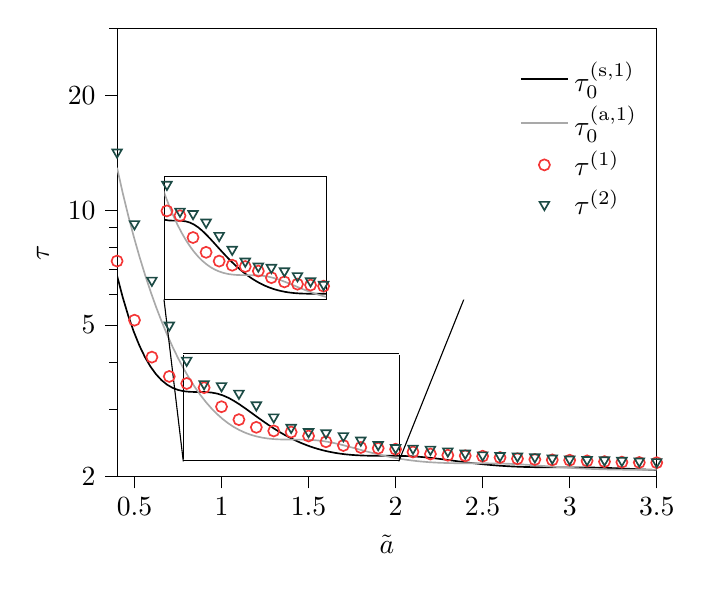
\begin{tikzpicture}

\definecolor{crimson2445454}{RGB}{244,54,54}
\definecolor{darkgray}{RGB}{169,169,169}
\definecolor{darkgray176}{RGB}{176,176,176}
\definecolor{darkslategray287569}{RGB}{28,75,69}

\begin{axis}[
legend cell align={left},
legend style={fill opacity=0.8, draw opacity=1, text opacity=1, at={(0.99,0.95)}, draw=none},
log basis y={10},
tick align=outside,
tick pos=left,
x grid style={darkgray176},
xlabel={\(\displaystyle \tilde{a}\)},
xmin=0.4, xmax=3.5,
xtick style={color=black},
y grid style={darkgray176},
ylabel={\(\displaystyle \tau\)},
ymin=2, ymax=30,
ymode=log,
ytick style={color=black},
log ticks with fixed point, %afegit a ma
ytick={2,5,10,20}, %afegit a ma
minor ytick={3,4,6,7,8,9,30} %afegit a ma
log ticks with fixed point, %afegit a ma
ytick={2,5,10,20}, %afegit a ma
minor ytick={3,4,6,7,8,9,30} %afegit a ma
]
\path [draw=black, very thin]
(axis cs:0.78,2.2)
--(axis cs:2.02,2.2);

\path [draw=black, very thin]
(axis cs:0.78,4.2)
--(axis cs:2.02,4.2);

\addplot [semithick, black]
table {%
0.4 6.72825292030247
0.432 5.91545229187631
0.464 5.28634768911461
0.496 4.7963421411059
0.528 4.41382951009721
0.56 4.11584473555358
0.592 3.88530443637343
0.624 3.70920029906621
0.656 3.57737918096583
0.688 3.48169197502918
0.72 3.41537700159799
0.752 3.37259296791516
0.784 3.34804790269751
0.816 3.33669479704719
0.848 3.33349139370581
0.88 3.33325966156223
0.912 3.33073157530565
0.944 3.32090257103383
0.976 3.29974467739081
1.008 3.26507155626806
1.04 3.21704435882346
1.072 3.15789236591412
1.104 3.09098926945622
1.136 3.01985541220195
1.168 2.9475167459249
1.2 2.87627377548193
1.232 2.80772899264669
1.264 2.74291813435254
1.296 2.6824556232774
1.328 2.62665822415478
1.36 2.57563908592478
1.392 2.52937532481947
1.424 2.48775507326301
1.456 2.45060957269139
1.488 2.41773469827627
1.52 2.38890511211673
1.552 2.36388328585707
1.584 2.34242493091744
1.616 2.32428187820386
1.648 2.3092031061096
1.68 2.29693438294397
1.712 2.28721683825132
1.744 2.27978469031944
1.776 2.27436233000581
1.808 2.27066100098259
1.84 2.26837544184565
1.872 2.26718109168218
1.904 2.26673282649373
1.936 2.26666666689641
1.968 2.26660634804295
2 2.26617674812126
2.032 2.26502539160133
2.064 2.26285103677499
2.096 2.2594348023592
2.128 2.25466582061739
2.16 2.24855263491284
2.192 2.24121531641575
2.224 2.23286023248796
2.256 2.22374541790808
2.288 2.21414614125772
2.32 2.2043275861464
2.352 2.19452726065865
2.384 2.18494634422811
2.416 2.17574758376365
2.448 2.16705718622216
2.48 2.15896868761904
2.512 2.15154745968379
2.544 2.1448350844609
2.576 2.1388532189681
2.608 2.13360680951658
2.64 2.12908664450602
2.672 2.12527129699727
2.704 2.12212853418087
2.736 2.1196162796304
2.768 2.1176832183426
2.8 2.11626914202972
2.832 2.11530514846053
2.864 2.1147138375684
2.896 2.1144096897957
2.928 2.11429986501649
2.96 2.11428571034752
2.992 2.11426528459169
3.024 2.11413715146644
3.056 2.11380551071437
3.088 2.11318639505667
3.12 2.112214202786
3.152 2.1108474137403
3.184 2.1090721878128
3.216 2.10690285892357
3.248 2.10437908292852
3.28 2.10156027789147
3.312 2.09851861393579
3.344 2.09533193468344
3.376 2.09207767569857
3.408 2.08882832862578
3.44 2.08564852538979
3.472 2.08259351219079
3.504 2.07970865719002
3.536 2.07702963552704
3.568 2.07458299812218
};
\addlegendentry{$\tau_0^{(\text{s},1)}$}
\addplot [semithick, darkgray]
table {%
0.4 12.9162306347444
0.432 11.1138365818156
0.464 9.67730849530524
0.496 8.51575913796571
0.528 7.56497601568763
0.56 6.7785486318439
0.592 6.12225708536105
0.624 5.57042056153321
0.656 5.10346066222428
0.688 4.70623864362572
0.72 4.36689782174188
0.752 4.07604299660612
0.784 3.82614917423807
0.816 3.61112908969108
0.848 3.42601249153608
0.88 3.2667052370696
0.912 3.1298061370274
0.944 3.0124660815167
0.976 2.91227844232942
1.008 2.82719281050617
1.04 2.7554462564738
1.072 2.69550779396016
1.104 2.64603278627069
1.136 2.60582478782342
1.168 2.5738028585519
1.2 2.54897279498128
1.232 2.53040105293274
1.264 2.5171904641607
1.296 2.5084572701833
1.328 2.503309655249
1.36 2.50082905874767
1.392 2.50005730761843
1.424 2.49999509528597
1.456 2.49961999149745
1.488 2.4979330737079
1.52 2.49403875875811
1.552 2.48724900820696
1.584 2.4771833106719
1.616 2.46382330317037
1.648 2.44749238234971
1.68 2.42876510982215
1.712 2.40834337800905
1.744 2.38694246821459
1.776 2.36521257989832
1.808 2.34369935085843
1.84 2.32283392974876
1.872 2.30294037307233
1.904 2.28425071029639
1.936 2.26692173385964
1.968 2.25105051737134
2 2.23668749640584
2.032 2.22384691035999
2.064 2.21251483266037
2.096 2.20265515882993
2.128 2.19421392897559
2.16 2.18712231511291
2.192 2.1812985452701
2.224 2.17664898481449
2.256 2.17306856026799
2.288 2.17044069781571
2.32 2.16863696320288
2.352 2.16751663777266
2.384 2.16692655197903
2.416 2.16670162120932
2.448 2.16666666975037
2.48 2.16664023292646
2.512 2.16644098988545
2.544 2.16589715232683
2.576 2.16485839465466
2.608 2.1632088075805
2.64 2.16087826566535
2.672 2.15784918360246
2.704 2.15415645066909
2.736 2.14988026687069
2.768 2.14513375196332
2.8 2.14004846305914
2.832 2.13476086454704
2.864 2.12940171813846
2.896 2.12408905353873
2.928 2.11892440630628
2.96 2.11399153860285
2.992 2.10935678505951
3.024 2.10507030442822
3.056 2.10116772061188
3.088 2.09767182360002
3.12 2.09459414287549
3.152 2.09193630203722
3.184 2.08969112355347
3.216 2.0878434883845
3.248 2.08637097666397
3.28 2.08524433024471
3.312 2.08442779111364
3.344 2.08387938517997
3.376 2.08355124084236
3.408 2.08339005601503
3.44 2.08333785250643
3.472 2.0833331741198
3.504 2.08331287912706
3.536 2.0832146275568
3.568 2.0829800486375
};
\addlegendentry{$\tau_0^{(\text{a},1)}$}
\addplot [semithick, crimson2445454, mark=o, mark size=2, mark options={solid,fill opacity=0}, only marks]
table {%
0.4 7.3508
0.5 5.1421
0.6 4.1141
0.7 3.661
0.8 3.509
0.9 3.4212
1 3.0495
1.1 2.8201
1.2 2.6926
1.3 2.6342
1.4 2.6165
1.5 2.5547
1.6 2.4674
1.7 2.4126
1.8 2.3838
1.9 2.3726
2 2.3589
2.1 2.3198
2.2 2.2913
2.3 2.2747
2.4 2.2671
2.5 2.2613
2.6 2.2436
2.7 2.2271
2.8 2.2166
2.9 2.2111
3 2.2074
3.1 2.1986
3.2 2.1885
3.3 2.1815
3.4 2.1773
3.5 2.1745
3.6 2.1695
3.7 2.1632
3.8 2.1582
3.9 2.155
4 2.1527
};
\addlegendentry{$\tau^{(1)}$}
\addplot [semithick, darkslategray287569, mark=triangle, mark size=2, mark options={solid,rotate=180,fill opacity=0}, only marks]
table {%
0.4 14.187
0.5 9.2002
0.6 6.5402
0.7 4.9881
0.8 4.0332
0.9 3.5006
1 3.4572
1.1 3.304
1.2 3.0794
1.3 2.8632
1.4 2.6895
1.5 2.6198
1.6 2.6023
1.7 2.5562
1.8 2.4904
1.9 2.4238
2 2.3785
2.1 2.3709
2.2 2.3566
2.3 2.3312
2.4 2.3009
2.5 2.2755
2.6 2.2679
2.7 2.2617
2.8 2.2499
2.9 2.2343
3 2.2197
3.1 2.213
3.2 2.2092
3.3 2.2029
3.4 2.1941
3.5 2.1852
3.6 2.1798
3.7 2.177
3.8 2.1731
3.9 2.1677
4 2.162
};
\addlegendentry{$\tau^{(2)}$}
\addplot [very thin, black, forget plot]
table {%
0.78 2.22881307097106
0.78 4.17759965032244
};
\addplot [very thin, black, forget plot]
table {%
2.02 2.22881307097106
2.02 4.17759965032244
};
\path [draw=black, fill=black]
(axis cs:0.67,5.8)
--(axis cs:0.67,5.8)
--(axis cs:0.670000499766753,5.80000001527065)
--(axis cs:0.780000499766753,2.20000001527065)
--(axis cs:0.779999500233247,2.19999998472935)
--(axis cs:0.669999500233247,5.79999998472935)
--(axis cs:0.67,5.8)
--cycle;
\path [draw=black, fill=black]
(axis cs:2.39,5.8)
--(axis cs:2.39,5.8)
--(axis cs:2.39000049737992,5.7999999488804)
--(axis cs:2.02000049737992,2.1999999488804)
--(axis cs:2.01999950262008,2.2000000511196)
--(axis cs:2.38999950262008,5.8000000511196)
--(axis cs:2.39,5.8)
--cycle;
\end{axis}

\begin{axis}[
log basis y={10},
xmajorticks=false,
xmin=0.78, xmax=2.02,
ymajorticks=false,
ymin=2.2, ymax=4.2,
ymode=log,
xshift=0.6cm,yshift=2.25cm,width=0.3\textwidth
]
\addplot [semithick, black]
table {%
0.4 6.72825292030247
0.432 5.91545229187631
0.464 5.28634768911461
0.496 4.7963421411059
0.528 4.41382951009721
0.56 4.11584473555358
0.592 3.88530443637343
0.624 3.70920029906621
0.656 3.57737918096583
0.688 3.48169197502918
0.72 3.41537700159799
0.752 3.37259296791516
0.784 3.34804790269751
0.816 3.33669479704719
0.848 3.33349139370581
0.88 3.33325966156223
0.912 3.33073157530565
0.944 3.32090257103383
0.976 3.29974467739081
1.008 3.26507155626806
1.04 3.21704435882346
1.072 3.15789236591412
1.104 3.09098926945622
1.136 3.01985541220195
1.168 2.9475167459249
1.2 2.87627377548193
1.232 2.80772899264669
1.264 2.74291813435254
1.296 2.6824556232774
1.328 2.62665822415478
1.36 2.57563908592478
1.392 2.52937532481947
1.424 2.48775507326301
1.456 2.45060957269139
1.488 2.41773469827627
1.52 2.38890511211673
1.552 2.36388328585707
1.584 2.34242493091744
1.616 2.32428187820386
1.648 2.3092031061096
1.68 2.29693438294397
1.712 2.28721683825132
1.744 2.27978469031944
1.776 2.27436233000581
1.808 2.27066100098259
1.84 2.26837544184565
1.872 2.26718109168218
1.904 2.26673282649373
1.936 2.26666666689641
1.968 2.26660634804295
2 2.26617674812126
2.032 2.26502539160133
2.064 2.26285103677499
2.096 2.2594348023592
2.128 2.25466582061739
2.16 2.24855263491284
2.192 2.24121531641575
2.224 2.23286023248796
2.256 2.22374541790808
2.288 2.21414614125772
2.32 2.2043275861464
2.352 2.19452726065865
2.384 2.18494634422811
2.416 2.17574758376365
2.448 2.16705718622216
2.48 2.15896868761904
2.512 2.15154745968379
2.544 2.1448350844609
2.576 2.1388532189681
2.608 2.13360680951658
2.64 2.12908664450602
2.672 2.12527129699727
2.704 2.12212853418087
2.736 2.1196162796304
2.768 2.1176832183426
2.8 2.11626914202972
2.832 2.11530514846053
2.864 2.1147138375684
2.896 2.1144096897957
2.928 2.11429986501649
2.96 2.11428571034752
2.992 2.11426528459169
3.024 2.11413715146644
3.056 2.11380551071437
3.088 2.11318639505667
3.12 2.112214202786
3.152 2.1108474137403
3.184 2.1090721878128
3.216 2.10690285892357
3.248 2.10437908292852
3.28 2.10156027789147
3.312 2.09851861393579
3.344 2.09533193468344
3.376 2.09207767569857
3.408 2.08882832862578
3.44 2.08564852538979
3.472 2.08259351219079
3.504 2.07970865719002
3.536 2.07702963552704
3.568 2.07458299812218
};
\addplot [semithick, darkgray]
table {%
0.4 12.9162306347444
0.432 11.1138365818156
0.464 9.67730849530524
0.496 8.51575913796571
0.528 7.56497601568763
0.56 6.7785486318439
0.592 6.12225708536105
0.624 5.57042056153321
0.656 5.10346066222428
0.688 4.70623864362572
0.72 4.36689782174188
0.752 4.07604299660612
0.784 3.82614917423807
0.816 3.61112908969108
0.848 3.42601249153608
0.88 3.2667052370696
0.912 3.1298061370274
0.944 3.0124660815167
0.976 2.91227844232942
1.008 2.82719281050617
1.04 2.7554462564738
1.072 2.69550779396016
1.104 2.64603278627069
1.136 2.60582478782342
1.168 2.5738028585519
1.2 2.54897279498128
1.232 2.53040105293274
1.264 2.5171904641607
1.296 2.5084572701833
1.328 2.503309655249
1.36 2.50082905874767
1.392 2.50005730761843
1.424 2.49999509528597
1.456 2.49961999149745
1.488 2.4979330737079
1.52 2.49403875875811
1.552 2.48724900820696
1.584 2.4771833106719
1.616 2.46382330317037
1.648 2.44749238234971
1.68 2.42876510982215
1.712 2.40834337800905
1.744 2.38694246821459
1.776 2.36521257989832
1.808 2.34369935085843
1.84 2.32283392974876
1.872 2.30294037307233
1.904 2.28425071029639
1.936 2.26692173385964
1.968 2.25105051737134
2 2.23668749640584
2.032 2.22384691035999
2.064 2.21251483266037
2.096 2.20265515882993
2.128 2.19421392897559
2.16 2.18712231511291
2.192 2.1812985452701
2.224 2.17664898481449
2.256 2.17306856026799
2.288 2.17044069781571
2.32 2.16863696320288
2.352 2.16751663777266
2.384 2.16692655197903
2.416 2.16670162120932
2.448 2.16666666975037
2.48 2.16664023292646
2.512 2.16644098988545
2.544 2.16589715232683
2.576 2.16485839465466
2.608 2.1632088075805
2.64 2.16087826566535
2.672 2.15784918360246
2.704 2.15415645066909
2.736 2.14988026687069
2.768 2.14513375196332
2.8 2.14004846305914
2.832 2.13476086454704
2.864 2.12940171813846
2.896 2.12408905353873
2.928 2.11892440630628
2.96 2.11399153860285
2.992 2.10935678505951
3.024 2.10507030442822
3.056 2.10116772061188
3.088 2.09767182360002
3.12 2.09459414287549
3.152 2.09193630203722
3.184 2.08969112355347
3.216 2.0878434883845
3.248 2.08637097666397
3.28 2.08524433024471
3.312 2.08442779111364
3.344 2.08387938517997
3.376 2.08355124084236
3.408 2.08339005601503
3.44 2.08333785250643
3.472 2.0833331741198
3.504 2.08331287912706
3.536 2.0832146275568
3.568 2.0829800486375
};
\addplot [semithick, crimson2445454, mark=o, mark size=2, mark options={solid,fill opacity=0}, only marks]
table {%
0.4 7.3508
0.5 5.1421
0.6 4.1141
0.7 3.661
0.8 3.509
0.9 3.4212
1 3.0495
1.1 2.8201
1.2 2.6926
1.3 2.6342
1.4 2.6165
1.5 2.5547
1.6 2.4674
1.7 2.4126
1.8 2.3838
1.9 2.3726
2 2.3589
2.1 2.3198
2.2 2.2913
2.3 2.2747
2.4 2.2671
2.5 2.2613
2.6 2.2436
2.7 2.2271
2.8 2.2166
2.9 2.2111
3 2.2074
3.1 2.1986
3.2 2.1885
3.3 2.1815
3.4 2.1773
3.5 2.1745
3.6 2.1695
3.7 2.1632
3.8 2.1582
3.9 2.155
4 2.1527
};
\addplot [semithick, darkslategray287569, mark=triangle, mark size=2, mark options={solid,rotate=180,fill opacity=0}, only marks]
table {%
0.4 14.187
0.5 9.2002
0.6 6.5402
0.7 4.9881
0.8 4.0332
0.9 3.5006
1 3.4572
1.1 3.304
1.2 3.0794
1.3 2.8632
1.4 2.6895
1.5 2.6198
1.6 2.6023
1.7 2.5562
1.8 2.4904
1.9 2.4238
2 2.3785
2.1 2.3709
2.2 2.3566
2.3 2.3312
2.4 2.3009
2.5 2.2755
2.6 2.2679
2.7 2.2617
2.8 2.2499
2.9 2.2343
3 2.2197
3.1 2.213
3.2 2.2092
3.3 2.2029
3.4 2.1941
3.5 2.1852
3.6 2.1798
3.7 2.177
3.8 2.1731
3.9 2.1677
4 2.162
};
\end{axis}

\end{tikzpicture}

% This file was created with tikzplotlib v0.10.1.
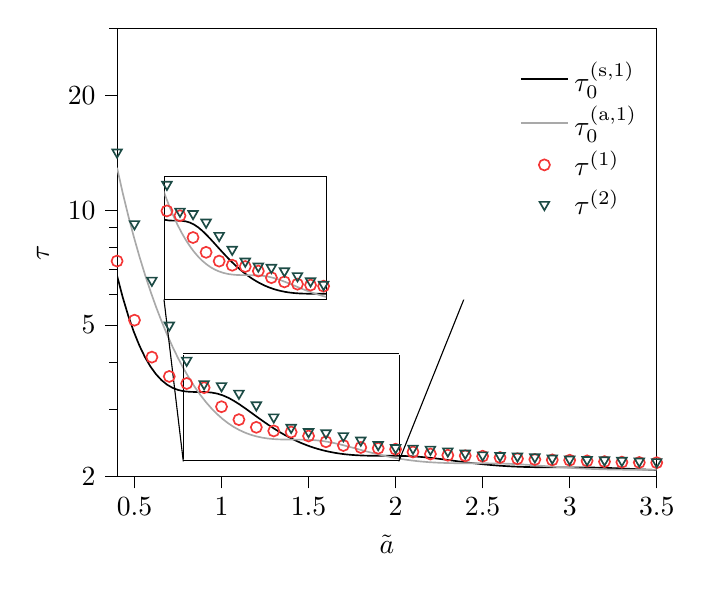
\begin{tikzpicture}

\definecolor{crimson2445454}{RGB}{244,54,54}
\definecolor{darkgray}{RGB}{169,169,169}
\definecolor{darkgray176}{RGB}{176,176,176}
\definecolor{darkslategray287569}{RGB}{28,75,69}

\begin{axis}[
legend cell align={left},
legend style={fill opacity=0.8, draw opacity=1, text opacity=1, at={(0.99,0.95)}, draw=none},
log basis y={10},
tick align=outside,
tick pos=left,
x grid style={darkgray176},
xlabel={\(\displaystyle \tilde{a}\)},
xmin=0.4, xmax=3.5,
xtick style={color=black},
y grid style={darkgray176},
ylabel={\(\displaystyle \tau\)},
ymin=2, ymax=30,
ymode=log,
ytick style={color=black},
log ticks with fixed point, %afegit a ma
ytick={2,5,10,20}, %afegit a ma
minor ytick={3,4,6,7,8,9,30} %afegit a ma
log ticks with fixed point, %afegit a ma
ytick={2,5,10,20}, %afegit a ma
minor ytick={3,4,6,7,8,9,30} %afegit a ma
]
\path [draw=black, very thin]
(axis cs:0.78,2.2)
--(axis cs:2.02,2.2);

\path [draw=black, very thin]
(axis cs:0.78,4.2)
--(axis cs:2.02,4.2);

\addplot [semithick, black]
table {%
0.4 6.72825292030247
0.432 5.91545229187631
0.464 5.28634768911461
0.496 4.7963421411059
0.528 4.41382951009721
0.56 4.11584473555358
0.592 3.88530443637343
0.624 3.70920029906621
0.656 3.57737918096583
0.688 3.48169197502918
0.72 3.41537700159799
0.752 3.37259296791516
0.784 3.34804790269751
0.816 3.33669479704719
0.848 3.33349139370581
0.88 3.33325966156223
0.912 3.33073157530565
0.944 3.32090257103383
0.976 3.29974467739081
1.008 3.26507155626806
1.04 3.21704435882346
1.072 3.15789236591412
1.104 3.09098926945622
1.136 3.01985541220195
1.168 2.9475167459249
1.2 2.87627377548193
1.232 2.80772899264669
1.264 2.74291813435254
1.296 2.6824556232774
1.328 2.62665822415478
1.36 2.57563908592478
1.392 2.52937532481947
1.424 2.48775507326301
1.456 2.45060957269139
1.488 2.41773469827627
1.52 2.38890511211673
1.552 2.36388328585707
1.584 2.34242493091744
1.616 2.32428187820386
1.648 2.3092031061096
1.68 2.29693438294397
1.712 2.28721683825132
1.744 2.27978469031944
1.776 2.27436233000581
1.808 2.27066100098259
1.84 2.26837544184565
1.872 2.26718109168218
1.904 2.26673282649373
1.936 2.26666666689641
1.968 2.26660634804295
2 2.26617674812126
2.032 2.26502539160133
2.064 2.26285103677499
2.096 2.2594348023592
2.128 2.25466582061739
2.16 2.24855263491284
2.192 2.24121531641575
2.224 2.23286023248796
2.256 2.22374541790808
2.288 2.21414614125772
2.32 2.2043275861464
2.352 2.19452726065865
2.384 2.18494634422811
2.416 2.17574758376365
2.448 2.16705718622216
2.48 2.15896868761904
2.512 2.15154745968379
2.544 2.1448350844609
2.576 2.1388532189681
2.608 2.13360680951658
2.64 2.12908664450602
2.672 2.12527129699727
2.704 2.12212853418087
2.736 2.1196162796304
2.768 2.1176832183426
2.8 2.11626914202972
2.832 2.11530514846053
2.864 2.1147138375684
2.896 2.1144096897957
2.928 2.11429986501649
2.96 2.11428571034752
2.992 2.11426528459169
3.024 2.11413715146644
3.056 2.11380551071437
3.088 2.11318639505667
3.12 2.112214202786
3.152 2.1108474137403
3.184 2.1090721878128
3.216 2.10690285892357
3.248 2.10437908292852
3.28 2.10156027789147
3.312 2.09851861393579
3.344 2.09533193468344
3.376 2.09207767569857
3.408 2.08882832862578
3.44 2.08564852538979
3.472 2.08259351219079
3.504 2.07970865719002
3.536 2.07702963552704
3.568 2.07458299812218
};
\addlegendentry{$\tau_0^{(\text{s},1)}$}
\addplot [semithick, darkgray]
table {%
0.4 12.9162306347444
0.432 11.1138365818156
0.464 9.67730849530524
0.496 8.51575913796571
0.528 7.56497601568763
0.56 6.7785486318439
0.592 6.12225708536105
0.624 5.57042056153321
0.656 5.10346066222428
0.688 4.70623864362572
0.72 4.36689782174188
0.752 4.07604299660612
0.784 3.82614917423807
0.816 3.61112908969108
0.848 3.42601249153608
0.88 3.2667052370696
0.912 3.1298061370274
0.944 3.0124660815167
0.976 2.91227844232942
1.008 2.82719281050617
1.04 2.7554462564738
1.072 2.69550779396016
1.104 2.64603278627069
1.136 2.60582478782342
1.168 2.5738028585519
1.2 2.54897279498128
1.232 2.53040105293274
1.264 2.5171904641607
1.296 2.5084572701833
1.328 2.503309655249
1.36 2.50082905874767
1.392 2.50005730761843
1.424 2.49999509528597
1.456 2.49961999149745
1.488 2.4979330737079
1.52 2.49403875875811
1.552 2.48724900820696
1.584 2.4771833106719
1.616 2.46382330317037
1.648 2.44749238234971
1.68 2.42876510982215
1.712 2.40834337800905
1.744 2.38694246821459
1.776 2.36521257989832
1.808 2.34369935085843
1.84 2.32283392974876
1.872 2.30294037307233
1.904 2.28425071029639
1.936 2.26692173385964
1.968 2.25105051737134
2 2.23668749640584
2.032 2.22384691035999
2.064 2.21251483266037
2.096 2.20265515882993
2.128 2.19421392897559
2.16 2.18712231511291
2.192 2.1812985452701
2.224 2.17664898481449
2.256 2.17306856026799
2.288 2.17044069781571
2.32 2.16863696320288
2.352 2.16751663777266
2.384 2.16692655197903
2.416 2.16670162120932
2.448 2.16666666975037
2.48 2.16664023292646
2.512 2.16644098988545
2.544 2.16589715232683
2.576 2.16485839465466
2.608 2.1632088075805
2.64 2.16087826566535
2.672 2.15784918360246
2.704 2.15415645066909
2.736 2.14988026687069
2.768 2.14513375196332
2.8 2.14004846305914
2.832 2.13476086454704
2.864 2.12940171813846
2.896 2.12408905353873
2.928 2.11892440630628
2.96 2.11399153860285
2.992 2.10935678505951
3.024 2.10507030442822
3.056 2.10116772061188
3.088 2.09767182360002
3.12 2.09459414287549
3.152 2.09193630203722
3.184 2.08969112355347
3.216 2.0878434883845
3.248 2.08637097666397
3.28 2.08524433024471
3.312 2.08442779111364
3.344 2.08387938517997
3.376 2.08355124084236
3.408 2.08339005601503
3.44 2.08333785250643
3.472 2.0833331741198
3.504 2.08331287912706
3.536 2.0832146275568
3.568 2.0829800486375
};
\addlegendentry{$\tau_0^{(\text{a},1)}$}
\addplot [semithick, crimson2445454, mark=o, mark size=2, mark options={solid,fill opacity=0}, only marks]
table {%
0.4 7.3508
0.5 5.1421
0.6 4.1141
0.7 3.661
0.8 3.509
0.9 3.4212
1 3.0495
1.1 2.8201
1.2 2.6926
1.3 2.6342
1.4 2.6165
1.5 2.5547
1.6 2.4674
1.7 2.4126
1.8 2.3838
1.9 2.3726
2 2.3589
2.1 2.3198
2.2 2.2913
2.3 2.2747
2.4 2.2671
2.5 2.2613
2.6 2.2436
2.7 2.2271
2.8 2.2166
2.9 2.2111
3 2.2074
3.1 2.1986
3.2 2.1885
3.3 2.1815
3.4 2.1773
3.5 2.1745
3.6 2.1695
3.7 2.1632
3.8 2.1582
3.9 2.155
4 2.1527
};
\addlegendentry{$\tau^{(1)}$}
\addplot [semithick, darkslategray287569, mark=triangle, mark size=2, mark options={solid,rotate=180,fill opacity=0}, only marks]
table {%
0.4 14.187
0.5 9.2002
0.6 6.5402
0.7 4.9881
0.8 4.0332
0.9 3.5006
1 3.4572
1.1 3.304
1.2 3.0794
1.3 2.8632
1.4 2.6895
1.5 2.6198
1.6 2.6023
1.7 2.5562
1.8 2.4904
1.9 2.4238
2 2.3785
2.1 2.3709
2.2 2.3566
2.3 2.3312
2.4 2.3009
2.5 2.2755
2.6 2.2679
2.7 2.2617
2.8 2.2499
2.9 2.2343
3 2.2197
3.1 2.213
3.2 2.2092
3.3 2.2029
3.4 2.1941
3.5 2.1852
3.6 2.1798
3.7 2.177
3.8 2.1731
3.9 2.1677
4 2.162
};
\addlegendentry{$\tau^{(2)}$}
\addplot [very thin, black, forget plot]
table {%
0.78 2.22881307097106
0.78 4.17759965032244
};
\addplot [very thin, black, forget plot]
table {%
2.02 2.22881307097106
2.02 4.17759965032244
};
\path [draw=black, fill=black]
(axis cs:0.67,5.8)
--(axis cs:0.67,5.8)
--(axis cs:0.670000499766753,5.80000001527065)
--(axis cs:0.780000499766753,2.20000001527065)
--(axis cs:0.779999500233247,2.19999998472935)
--(axis cs:0.669999500233247,5.79999998472935)
--(axis cs:0.67,5.8)
--cycle;
\path [draw=black, fill=black]
(axis cs:2.39,5.8)
--(axis cs:2.39,5.8)
--(axis cs:2.39000049737992,5.7999999488804)
--(axis cs:2.02000049737992,2.1999999488804)
--(axis cs:2.01999950262008,2.2000000511196)
--(axis cs:2.38999950262008,5.8000000511196)
--(axis cs:2.39,5.8)
--cycle;
\end{axis}

\begin{axis}[
log basis y={10},
xmajorticks=false,
xmin=0.78, xmax=2.02,
ymajorticks=false,
ymin=2.2, ymax=4.2,
ymode=log,
xshift=0.6cm,yshift=2.25cm,width=0.3\textwidth
]
\addplot [semithick, black]
table {%
0.4 6.72825292030247
0.432 5.91545229187631
0.464 5.28634768911461
0.496 4.7963421411059
0.528 4.41382951009721
0.56 4.11584473555358
0.592 3.88530443637343
0.624 3.70920029906621
0.656 3.57737918096583
0.688 3.48169197502918
0.72 3.41537700159799
0.752 3.37259296791516
0.784 3.34804790269751
0.816 3.33669479704719
0.848 3.33349139370581
0.88 3.33325966156223
0.912 3.33073157530565
0.944 3.32090257103383
0.976 3.29974467739081
1.008 3.26507155626806
1.04 3.21704435882346
1.072 3.15789236591412
1.104 3.09098926945622
1.136 3.01985541220195
1.168 2.9475167459249
1.2 2.87627377548193
1.232 2.80772899264669
1.264 2.74291813435254
1.296 2.6824556232774
1.328 2.62665822415478
1.36 2.57563908592478
1.392 2.52937532481947
1.424 2.48775507326301
1.456 2.45060957269139
1.488 2.41773469827627
1.52 2.38890511211673
1.552 2.36388328585707
1.584 2.34242493091744
1.616 2.32428187820386
1.648 2.3092031061096
1.68 2.29693438294397
1.712 2.28721683825132
1.744 2.27978469031944
1.776 2.27436233000581
1.808 2.27066100098259
1.84 2.26837544184565
1.872 2.26718109168218
1.904 2.26673282649373
1.936 2.26666666689641
1.968 2.26660634804295
2 2.26617674812126
2.032 2.26502539160133
2.064 2.26285103677499
2.096 2.2594348023592
2.128 2.25466582061739
2.16 2.24855263491284
2.192 2.24121531641575
2.224 2.23286023248796
2.256 2.22374541790808
2.288 2.21414614125772
2.32 2.2043275861464
2.352 2.19452726065865
2.384 2.18494634422811
2.416 2.17574758376365
2.448 2.16705718622216
2.48 2.15896868761904
2.512 2.15154745968379
2.544 2.1448350844609
2.576 2.1388532189681
2.608 2.13360680951658
2.64 2.12908664450602
2.672 2.12527129699727
2.704 2.12212853418087
2.736 2.1196162796304
2.768 2.1176832183426
2.8 2.11626914202972
2.832 2.11530514846053
2.864 2.1147138375684
2.896 2.1144096897957
2.928 2.11429986501649
2.96 2.11428571034752
2.992 2.11426528459169
3.024 2.11413715146644
3.056 2.11380551071437
3.088 2.11318639505667
3.12 2.112214202786
3.152 2.1108474137403
3.184 2.1090721878128
3.216 2.10690285892357
3.248 2.10437908292852
3.28 2.10156027789147
3.312 2.09851861393579
3.344 2.09533193468344
3.376 2.09207767569857
3.408 2.08882832862578
3.44 2.08564852538979
3.472 2.08259351219079
3.504 2.07970865719002
3.536 2.07702963552704
3.568 2.07458299812218
};
\addplot [semithick, darkgray]
table {%
0.4 12.9162306347444
0.432 11.1138365818156
0.464 9.67730849530524
0.496 8.51575913796571
0.528 7.56497601568763
0.56 6.7785486318439
0.592 6.12225708536105
0.624 5.57042056153321
0.656 5.10346066222428
0.688 4.70623864362572
0.72 4.36689782174188
0.752 4.07604299660612
0.784 3.82614917423807
0.816 3.61112908969108
0.848 3.42601249153608
0.88 3.2667052370696
0.912 3.1298061370274
0.944 3.0124660815167
0.976 2.91227844232942
1.008 2.82719281050617
1.04 2.7554462564738
1.072 2.69550779396016
1.104 2.64603278627069
1.136 2.60582478782342
1.168 2.5738028585519
1.2 2.54897279498128
1.232 2.53040105293274
1.264 2.5171904641607
1.296 2.5084572701833
1.328 2.503309655249
1.36 2.50082905874767
1.392 2.50005730761843
1.424 2.49999509528597
1.456 2.49961999149745
1.488 2.4979330737079
1.52 2.49403875875811
1.552 2.48724900820696
1.584 2.4771833106719
1.616 2.46382330317037
1.648 2.44749238234971
1.68 2.42876510982215
1.712 2.40834337800905
1.744 2.38694246821459
1.776 2.36521257989832
1.808 2.34369935085843
1.84 2.32283392974876
1.872 2.30294037307233
1.904 2.28425071029639
1.936 2.26692173385964
1.968 2.25105051737134
2 2.23668749640584
2.032 2.22384691035999
2.064 2.21251483266037
2.096 2.20265515882993
2.128 2.19421392897559
2.16 2.18712231511291
2.192 2.1812985452701
2.224 2.17664898481449
2.256 2.17306856026799
2.288 2.17044069781571
2.32 2.16863696320288
2.352 2.16751663777266
2.384 2.16692655197903
2.416 2.16670162120932
2.448 2.16666666975037
2.48 2.16664023292646
2.512 2.16644098988545
2.544 2.16589715232683
2.576 2.16485839465466
2.608 2.1632088075805
2.64 2.16087826566535
2.672 2.15784918360246
2.704 2.15415645066909
2.736 2.14988026687069
2.768 2.14513375196332
2.8 2.14004846305914
2.832 2.13476086454704
2.864 2.12940171813846
2.896 2.12408905353873
2.928 2.11892440630628
2.96 2.11399153860285
2.992 2.10935678505951
3.024 2.10507030442822
3.056 2.10116772061188
3.088 2.09767182360002
3.12 2.09459414287549
3.152 2.09193630203722
3.184 2.08969112355347
3.216 2.0878434883845
3.248 2.08637097666397
3.28 2.08524433024471
3.312 2.08442779111364
3.344 2.08387938517997
3.376 2.08355124084236
3.408 2.08339005601503
3.44 2.08333785250643
3.472 2.0833331741198
3.504 2.08331287912706
3.536 2.0832146275568
3.568 2.0829800486375
};
\addplot [semithick, crimson2445454, mark=o, mark size=2, mark options={solid,fill opacity=0}, only marks]
table {%
0.4 7.3508
0.5 5.1421
0.6 4.1141
0.7 3.661
0.8 3.509
0.9 3.4212
1 3.0495
1.1 2.8201
1.2 2.6926
1.3 2.6342
1.4 2.6165
1.5 2.5547
1.6 2.4674
1.7 2.4126
1.8 2.3838
1.9 2.3726
2 2.3589
2.1 2.3198
2.2 2.2913
2.3 2.2747
2.4 2.2671
2.5 2.2613
2.6 2.2436
2.7 2.2271
2.8 2.2166
2.9 2.2111
3 2.2074
3.1 2.1986
3.2 2.1885
3.3 2.1815
3.4 2.1773
3.5 2.1745
3.6 2.1695
3.7 2.1632
3.8 2.1582
3.9 2.155
4 2.1527
};
\addplot [semithick, darkslategray287569, mark=triangle, mark size=2, mark options={solid,rotate=180,fill opacity=0}, only marks]
table {%
0.4 14.187
0.5 9.2002
0.6 6.5402
0.7 4.9881
0.8 4.0332
0.9 3.5006
1 3.4572
1.1 3.304
1.2 3.0794
1.3 2.8632
1.4 2.6895
1.5 2.6198
1.6 2.6023
1.7 2.5562
1.8 2.4904
1.9 2.4238
2 2.3785
2.1 2.3709
2.2 2.3566
2.3 2.3312
2.4 2.3009
2.5 2.2755
2.6 2.2679
2.7 2.2617
2.8 2.2499
2.9 2.2343
3 2.2197
3.1 2.213
3.2 2.2092
3.3 2.2029
3.4 2.1941
3.5 2.1852
3.6 2.1798
3.7 2.177
3.8 2.1731
3.9 2.1677
4 2.162
};
\end{axis}

\end{tikzpicture}

	\caption{Critical compression of a stiffened inhomogeneous sheet ($\phi_{-a}=0.2,\gamma\prime=10$) as a function of the size $\ta$, with numerical results from {\it Chebfun}~\cite{Chebfun} ($\tauu,\taud$). Quantities $\tau_0^{(\text{s},1)}$, $\tau_0^{(\text{a},1)}$ denote the smallest pair of compressions of the corresponding homogeneous sheet ($\phi_{-a}=0$).}
\label{soft-res:tau}
\end{figure}

We show in Fig.~\ref{soft-res:tau} the splitting between the two lowest compressions of the inhomogeneous sheet, denoted $\tauu(\tilde{a})$ and $\taud(\tilde{a})$, with $\tauu(\tilde{a})<\taud(\tilde{a})$. Let  $\Delta\tau^{(2-1)}\equiv\tau^{(2)}-\tau^{(1)}$ be the separation between neighbouring compressive loads. For a homogeneous sheet, it vanishes at certain values of $\ta$ given by the crossing points from Eqs.~\eqref{finite-size:crossing1} and \eqref{finite-size:crossing2}. We see in Fig.~\ref{soft-res:tau} that $\Delta\tau^{(2-1)}$ never vanishes in the inhomogeneous case, but still has a local minima around every crossing point. We next examine the growth of $\Delta\tau^{(2-1)}$ with $\phi_{-a}$. 

We fix $\phi_{-a}$ and then we find numerically the local minima of $\Delta\tau^{(2-1)}$ with respect to $\ta$, which we denote $\Delta\tau^{(2-1)}_{\text{min}}$. The values of $\ta$ that minimize $\Delta\tau^{(2-1)}$ start at the crossing points when $\phi_{-a}=0$, and increase with $\phi_{-a}$. The first eight results $\Delta\tau^{(2-1)}_{\text{min}}$ (corresponding to the first eight crossings in the homogeneous case) are plotted in Fig.~\ref{soft-res:dtmin} for different values of $\phi_{-a}/a$, where $a$ is the corresponding sheet size that minimizes $\Delta\tau^{(2-1)}$. All curves $\Delta\tau^{(2-1)}_{\text{min}}$ collapse into one, therefore we conclude that $\Delta\tau^{(2-1)}_{\text{min}}$ grows linearly with $\phi_{-a}/a$, which is twice the amplitude of the gradient from Eq.~\eqref{buckle:phi}.
%Rescaling $\phi_{-a}$ by $a$, where $a$ is the corresponding sheet size that minimizes $\Delta\tau^{(2-1)}$, all curves $\Delta\tau^{(2-1)}_{\text{min}}$ collapse into one. We therefore conclude that $\Delta\tau^{(2-1)}_{\text{min}}$ grows linearly with $\phi_{-a}/a$, which is twice the amplitude of the gradient from Eq.~\eqref{buckle:phi}.
%________________________________________________________________________________________________________________________________________________________________________________________________________________

\begin{figure}
	%\includegraphics[width=\columnwidth]{figures/Fig_epsilon/plDeltatauMinNUMscaledLog.eps}
	\includegraphics[width=\columnwidth]{plDeltatauMinNUMscaledLog.eps}
	\caption{Minimal separation between the two lowest compressions $\bigl(\tau^{(1)},\tau^{(2)}\bigr)$ of a stiffened inhomogeneous sheet ($\gamma\prime=10$). Different symbols denote those minima corresponding to the crossings of type I (circles), and of type II (triangles) when $\phi_{-a}=0$. Shades of gray correspond to the crossing point index $l$: lighter gray for $l=1$, darkest gray for $l=4$. The red right triangle is one decade in length on both legs, and hence enlightens the linear relation $\Delta\tau\propto\phi_{-a}/a$.}
\label{soft-res:dtmin}
\end{figure}


\subsection{Buckling profiles of medium length sheets\label{soft-res-profiles}}
For medium length sheets [$\ta=O(1,10)$], we examine the buckling profiles corresponding to the lowest compression, $\tau^{(1)}$. The contour plot of $w(x)$ in Fig.~\ref{soft-res:profiles} shows how the buckling profiles are no longer symmetric and the largest deflections (i.e. those brighter/darker areas) tend to be located towards the softer side of the sheet ($x>0$). This intuitive feature is also observed in the buckling profiles of an inhomogeneous column~\cite{SuneWettlaufer21}.

\begin{figure}
	%\includegraphics[width=\columnwidth]{figures/Fig_profiles/figprofilesNUMredsize.eps}
	%\includegraphics[width=\columnwidth]{figures/Fig_profiles/figprofilesNUM-d002L-redsize.eps}
	\includegraphics[width=\columnwidth]{figprofilesNUM-d002L-redsize.eps}
	\caption{Contour plots for $w(x)$ with varying $\ta$ and the largest vertical displacement (highlighted in green), for a medium length stiffened sheet. Here, $\phi_{-a}=0.1,\gamma\prime=10$, $d=L/50,$ and $\mathcal{S}\approx 300$ to compute the amplitudes via Eqs.~\eqref{homogeneous:intrel} and~\eqref{homogeneous:ampls}.}
\label{soft-res:profiles}
\end{figure}

Despite the lack of symmetry, the buckling profiles of a medium length inhomogeneous sheet are similar to the fundamental symmetric/antisymmetric modes characteristic of the homogeneous sheets. We project the numerical solutions for the inhomogeneous sheet, $w(x)$, onto the modes of the homogeneous sheet (Eqs.~\ref{homogeneous:sols}), i.e. the basis of eigenfunctions of the eigenvalue problem given by Eq.~\eqref{homogeneous:ode0} \footnote{Integration by parts shows that the operators $\left(\frac{\mathrm{d}^4}{\mathrm{d}x^4}+1\right)$ and $\left(-\frac{\mathrm{d}^2}{\mathrm{d}x^2}\right)$ are Hermitian, the latter is also positive definite, and hence $\{\left(\frac{\mathrm{d}^4}{\mathrm{d}x^4}+1\right),\left(-\frac{\mathrm{d}^2}{\mathrm{d}x^2}\right)\}$ is a Hermitian definite pencil. Therefore, the problem is one of standard Hermitian eigen-theory and we can take advantage of the completeness of the known eigenfunctions, Eqs. \eqref{homogeneous:sole} and \eqref{homogeneous:solo}, of the homogeneous sheet problem, Eq.~\eqref{homogeneous:ode0}.}. More concretely, we expand the solution of Eq.~\eqref{buckle:ode} as the infinite linear combination
\begin{align}
	%w(x)=\sum_{n=0}^{\infty} a_n w_0^{(n)}(x), 
	w(x)=\sum_{j=1}^{\infty} \left[\mathrm{a}_j^{\text{(s)}} w_0^{(\text{s},j)}(x)+\mathrm{a}_j^{\text{(a)}} w_0^{(\text{a},j)}(x)\right], 
	\label{soft-res:complete}
\end{align}
where we use the same index $j$ to denote each pair of solutions --symmetric (s) and antisymmetric (a)-- as in the homogeneous sheet. We redefine the eigenfunctions~\eqref{homogeneous:sole} and ~\eqref{homogeneous:solo} as
\begin{align}
	w_0^{(\text{s})}(x)&=\cos k_-a\,\cos k_+x-\cos k_-x\,\cos k_+a,\label{soft-res:sole}\\
	\text{and}\quad w_0^{(\text{a})}(x)&=\sin k_-a\sin k_+x-\sin k_-x\sin k_+a.
\label{soft-res:solo}
\end{align}

The function $w(x)$ is normalized via the inextensibility constraint~\footnote{The inner product is on the Hilbert space of eigenfunctions $w_0^{(n)}$, so that the basis of eigenfunctions are orthogonal.},
\begin{align}
\int_{-a}^{a}\left(\frac{\mathrm{d}w}{\mathrm{d}x}\right)^2\mathrm{~d}x=1.\label{soft-res:norm}
\end{align} 
The coefficients $\mathrm{a}_1^{\text{(s)}}$ and $\mathrm{a}_1^{\text{(a)}}$ are plotted in Fig.~\ref{soft-res:coeffs}. The first pair of modes --- either the symmetric or the antisymmetric --- are dominant in the linear combination that describes $w(x)$. This dominant term changes in the vicinity of the crossing points (depicted by vertical dashed lines in Fig.~\ref{soft-res:coeffs}). 
However, for larger and more inhomogeneous sheets the sum $\Big[\mathrm{a}_1^{\text{(s)}}\Big]^2+\Big[\mathrm{a}_1^{\text{(a)}}\Big]^2$, plotted in Fig.~\ref{soft-res:product}, is smaller than unity.
(Those cases with larger values of $\phi_{-a}$ are plotted in lighter gray in Figs.~\ref{soft-res:coeffs} and~\ref{soft-res:product}.)
This indicates a reduction in the projection of $w(x)$ onto the first pair of modes.
\begin{figure}
	%\includegraphics[width=\columnwidth]{figures/fig_modes_PDMS/figcoeffRNNUM.eps}
	\includegraphics[width=\columnwidth]{figcoeffRNNUM.eps}
	\caption{Lowest pair of squared coefficients in the expansion~\eqref{soft-res:complete} for a stiffened inhomogeneous sheet ($\gamma\prime=10$). Solid curves denote $\Big[\mathrm{a}_1^{(\text{s})}\Big]^2$, and dotted curves $\Big[\mathrm{a}_1^{(\text{a})}\Big]^2$, with different shades of gray for trajectories corresponding to each value of $\phi_{-a}$, from $\phi_{-a}=0.02$ (black), to $\phi_{-a}=0.2$ (lightest gray), and equally spaced jumps for the curves in between. The dashed vertical lines denote the crossing points as in Eq.~\eqref{finite-size:crossing1} and~\eqref{finite-size:crossing2} ($j=1,l=\{1,2,3,4\}$).}
\label{soft-res:coeffs}
\end{figure}
Higher order modes are necessary to account for the buckling profile of longer and more inhomogeneous sheets. Thus the difference between the wrinkles in homogeneous and inhomogeneous sheets increases. A rationale behind this result is found in the compression graph [Fig.~\ref{finite-size:modes}~(a)] of a homogeneous sheet: all buckling modes converge towards $\tau=2$ in the limit of large sheets ($\ta\gg 1$), and so they contribute similarly to the buckling profile. As $\tau\to 2$ the wavenumbers defining the different modes in the homogeneous sheet tend to accumulate at unity, see Fig.~\ref{homogeneous:wavenums}.

\begin{figure}
%% This file was created with tikzplotlib v0.10.1.
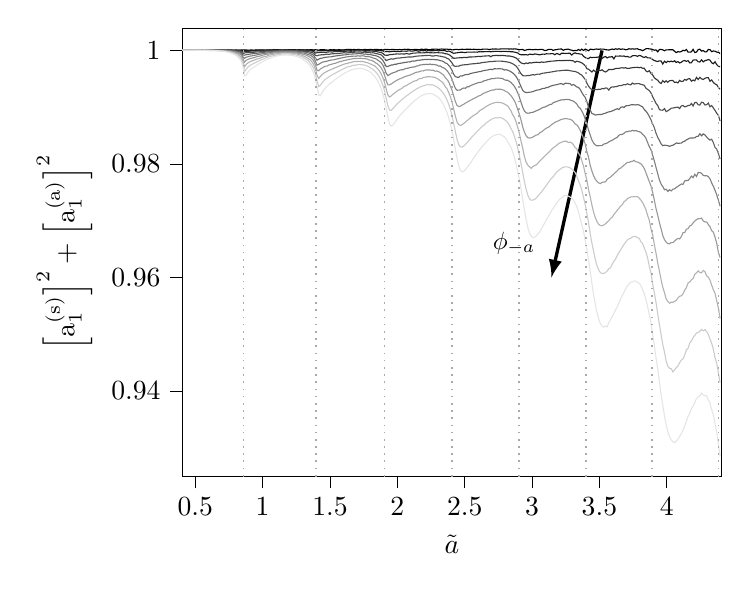
\begin{tikzpicture}

\definecolor{black25}{RGB}{25,25,25}
\definecolor{darkgray}{RGB}{169,169,169}
\definecolor{darkgray153}{RGB}{153,153,153}
\definecolor{darkgray176}{RGB}{176,176,176}
\definecolor{darkgray178}{RGB}{178,178,178}
\definecolor{darkslategray51}{RGB}{51,51,51}
\definecolor{darkslategray76}{RGB}{76,76,76}
\definecolor{dimgray102}{RGB}{102,102,102}
\definecolor{gainsboro229}{RGB}{229,229,229}
\definecolor{lightgray204}{RGB}{204,204,204}

\begin{axis}[
tick align=outside,
tick pos=left,
x grid style={darkgray176},
xlabel={\(\displaystyle \tilde{a}\)},
xmin=1, xmax=321,
xtick style={color=black},
xtick={8.8125,48.75,88.6875,128.625,168.5625,208.5,248.4375,288.375},
xticklabels={
  \(\displaystyle 0.5\),
  \(\displaystyle 1\),
  \(\displaystyle 1.5\),
  \(\displaystyle 2\),
  \(\displaystyle 2.5\),
  \(\displaystyle 3\),
  \(\displaystyle 3.5\),
  \(\displaystyle 4\)
},
y grid style={darkgray176},
ylabel={\(\displaystyle \Big[\mathrm{a}_1^{(\text{s})}\Big]^2+\Big[\mathrm{a}_1^{(\text{a})}\Big]^2\)},
ymin=0.924921672391509, ymax=1.00391663709987,
ytick style={color=black}
]
\draw[-latex,very thick,draw=black] (axis cs:250,1) -- (axis cs:220,0.96);
\addplot [black]
table {%
0 1.00006636262959
1 1.00005763051523
2 1.000057703946
3 1.00006044864142
4 1.00005787604676
5 1.00005797611006
6 1.00005808479128
7 1.00005820152389
8 1.00005832727063
9 1.00005846522253
10 1.0000586130052
11 1.00005877202897
12 1.00005894635015
13 1.00005912997859
14 1.00005932626032
15 1.0000595394729
16 1.00005976578295
17 1.00006000503969
18 1.00006025993993
19 1.0000605291046
20 1.0000608124279
21 1.00007057196262
22 1.00004904467763
23 1.00007135450139
24 1.00007177070861
25 1.00006240097976
26 1.0000627363479
27 1.00006306850758
28 1.00007353941458
29 1.00004609516445
30 1.00007440191715
31 1.00004214527282
32 1.00004583271438
33 1.00007540586732
34 1.0000676785184
35 1.00004897085546
36 1.00007424170824
37 1.00008597718007
38 1.00008882076773
39 1.00009012636972
40 1.00004863413332
41 1.00005628472667
42 1.00009395087359
43 1.00005887145359
44 1.00005375578436
45 1.00009845508488
46 1.00005672905998
47 1.00010175661121
48 1.00010343975098
49 1.00010511833047
50 1.00006285450661
51 1.00007097918798
52 1.00010994711013
53 1.00011144667844
54 1.00011287845566
55 1.00011424346992
56 1.00011553969638
57 1.00011677019933
58 1.00011793869094
59 1.00008019963575
60 1.00008102754868
61 1.00007477266361
62 1.0001220905885
63 1.00008313682732
64 1.00012390945709
65 1.00012476399357
66 1.00012558314445
67 1.00012636700969
68 1.00012711226918
69 1.00008577765681
70 1.00012847119968
71 1.00012907228942
72 1.00008611679984
73 1.00010506221726
74 1.00008579313205
75 1.00013067715198
76 1.00008478346559
77 1.0001305277576
78 1.00012962121494
79 1.00008597026767
80 1.00013257580669
81 1.00007960644881
82 1.0000615969099
83 1.00014232619709
84 1.00012580725101
85 1.00014559294385
86 1.00008717067652
87 1.0000684008629
88 1.00006998673868
89 1.00015315303042
90 1.00009406981846
91 1.00015755074491
92 1.00008703112988
93 1.00007922822748
94 1.00016468920629
95 1.00010439012259
96 1.0001065184598
97 1.00008726438332
98 1.00015508019267
99 1.00017685610324
100 1.00016939907707
101 1.00017159201404
102 1.00014648481008
103 1.00017573197854
104 1.00012139822742
105 1.0001794946742
106 1.00018122130071
107 1.00012526062262
108 1.00010324152959
109 1.00018571395309
110 1.0001672020581
111 1.00012841294042
112 1.00015947732103
113 1.0001788881636
114 1.00010449831362
115 1.00017003682906
116 1.00019096946404
117 1.00019070885523
118 1.0000996049641
119 1.00016517676183
120 1.00007895927341
121 1.00017132483517
122 1.00015508861522
123 1.00018393330387
124 1.00012784656066
125 1.00016269397988
126 1.00017665844959
127 1.00015451489356
128 1.0001565775296
129 1.00011865243378
130 1.00017344839017
131 1.00010631362597
132 1.00017864290291
133 1.00020830469742
134 1.00018435346185
135 1.0002145188268
136 1.00015557243688
137 1.00013898792293
138 1.00014187227995
139 1.00018704885437
140 1.00019015996431
141 1.00010963457818
142 1.00013539405652
143 1.00024088870132
144 1.00014032419805
145 1.00021810573561
146 1.00022073121685
147 1.000130272871
148 1.00011665624614
149 1.00021369193478
150 1.00021549213669
151 1.00023107300872
152 1.00023245724536
153 1.00015311547807
154 1.00023433876202
155 1.00024921462944
156 1.00021993345851
157 1.00021905963031
158 1.00023210611046
159 1.00018569850625
160 1.00020864428228
161 1.00010447001941
162 1.00011978656196
163 1.0001977845859
164 1.00020105708796
165 1.00012996004098
166 1.00018861100256
167 1.00020832263596
168 1.00019318664513
169 1.00019565008179
170 1.00021600968756
171 1.00020110682695
172 1.00020412546374
173 1.00019182325536
174 1.00021074168218
175 1.00018275421018
176 1.0001584637605
177 1.00019001828215
178 1.00014080313644
179 1.00021391003569
180 1.00023400251374
181 1.00023809006779
182 1.00024214749934
183 1.00013592688407
184 1.00021684727545
185 1.00025380361605
186 1.00024070900228
187 1.00026080130532
188 1.00022990348597
189 1.0002325709129
190 1.00026948305142
191 1.00027175905756
192 1.00027366060598
193 1.00027513974552
194 1.00027612590854
195 1.00024058612607
196 1.0002761085409
197 1.0002379563511
198 1.00027067094417
199 1.00026071037875
200 1.00018237060725
201 1.00014396299986
202 1.00015731701043
203 1.00016322936997
204 0.999993579224106
205 1.0000860577673
206 1.00017125454772
207 1.00017336900737
208 1.00015596294003
209 1.00012380780063
210 1.00016076891717
211 1.0001635419882
212 1.00013165201996
213 1.00016991353877
214 1.00019369097378
215 1.00014193020147
216 0.99999147197028
217 1.00002206751231
218 1.00015430565415
219 1.0001949151317
220 1.00019965089311
221 1.00000092802118
222 1.0001110777665
223 1.00014437165664
224 1.00021866896926
225 1.00024456789974
226 1.00024902820634
227 1.0000210397115
228 1.00016370726736
229 1.00020058534135
230 1.00024191157888
231 1.00011357459263
232 1.00004712509535
233 0.999933547584059
234 1.00001129462547
235 0.999966998042594
236 1.00017073620339
237 0.999999689548183
238 1.00023341003352
239 0.9999977107331
240 1.00023661707014
241 1.00011346179308
242 0.999946526222487
243 1.00023688591083
244 1.00018237351745
245 1.00013182252021
246 1.00024482691912
247 1.00024699734233
248 1.00019047734346
249 1.00025189814645
250 1.00022294158559
251 1.00022608340838
252 1.00014739422884
253 1.00010493452624
254 1.00006755684024
255 1.00015937869141
256 1.00024767913824
257 1.00014572887107
258 1.00029181796761
259 1.0002070313223
260 1.00030421313782
261 1.00019138655568
262 1.00025430373288
263 1.00023085595666
264 1.00011725705761
265 1.00016605055543
266 1.00030815846705
267 1.00022530900096
268 1.0002889892423
269 1.00023464250169
270 1.0002669799135
271 1.00030148243391
272 1.00014826516445
273 1.00010857678252
274 0.999958465290203
275 1.00010538575539
276 1.00030256924677
277 1.00032595688585
278 1.00027349148822
279 1.00024686053061
280 1.00016915132976
281 1.00003817792041
282 1.00010259540318
283 0.999758762753217
284 1.00017592958983
285 1.00017723419563
286 1.00010889182797
287 0.999946493128583
288 1.00011129995275
289 1.00011298397478
290 1.00011520389464
291 1.00011824237298
292 1.00012127671229
293 0.999855635605281
294 0.999623080593992
295 0.999797356770517
296 0.999725672958191
297 0.999805765890238
298 1.00003124338681
299 0.999940103249752
300 1.00016572492063
301 0.999708206912347
302 0.999695167310477
303 0.999759859451902
304 1.00019486469087
305 0.999629372866293
306 0.999714143512221
307 1.00014811919022
308 1.00022118811301
309 0.999882907545284
310 0.999979664468639
311 0.999746472517758
312 0.999767269483091
313 1.00017026074638
314 1.00013614381134
315 0.999791724691682
316 0.999903923879752
317 0.999863779356213
318 0.999702829463224
319 0.999671213074256
320 0.99946222101835
};
\addplot [black25]
table {%
0 1.00006326437676
1 1.00005024621788
2 1.00006647942666
3 1.00006656380826
4 1.00006665342258
5 1.00004637827345
6 1.00004449090588
7 1.00006696238074
8 1.00005815080909
9 1.00006719165237
10 1.000064189161
11 1.00006115002624
12 1.0000675584863
13 1.00004314881934
14 1.00006779774765
15 1.00004317703511
16 1.00004490957263
17 1.00006487550933
18 1.00004480137279
19 1.00005883546263
20 1.00004272223668
21 1.00005073040096
22 1.00006125703086
23 1.00006095739084
24 1.00006730695172
25 1.00005701097781
26 1.00004120429666
27 1.00003808791625
28 1.00005690177414
29 1.00005525055048
30 1.00005315871277
31 1.00005792995071
32 1.00005475128137
33 1.00002543604502
34 1.00002211460733
35 1.00003825874613
36 1.00002400989592
37 0.999967850376115
38 0.999993270886021
39 0.999971005406477
40 0.999984229488614
41 0.99997322825127
42 0.999978007232052
43 1.00001949567521
44 1.00002579682132
45 1.00003037344021
46 1.00003606446231
47 1.00004182870133
48 1.00004855178492
49 1.00005322865837
50 1.0000587039076
51 1.00006392383945
52 1.00003890200256
53 1.0000734186647
54 1.00004743345101
55 1.0000511187222
56 1.00008487781465
57 1.0000879268899
58 1.00009059611882
59 1.00008109882062
60 1.00006369659363
61 1.00006509313535
62 1.00006613161656
63 1.00008647722808
64 1.00005902164765
65 1.00009933826212
66 1.00009916373448
67 1.00005353105489
68 1.00009760440594
69 1.00003134559046
70 1.00009418234853
71 1.00009164283365
72 1.00008188846413
73 1.00007787827708
74 1.0000442157115
75 1.00007383608399
76 1.00005259846938
77 1.00001049160283
78 1.00004295057595
79 0.999989414564777
80 0.999906428743849
81 0.999909828730634
82 0.999969044948784
83 0.999935363627039
84 0.999981129193402
85 0.999977036060047
86 0.99999111803856
87 0.99997801825051
88 0.999941308664935
89 0.999998558115313
90 1.00001395361839
91 0.99995896150287
92 1.00000828020339
93 1.00003384157345
94 1.00004069501877
95 0.999984875914981
96 1.00005426188592
97 1.00004154812895
98 1.00005743406267
99 1.0000730223881
100 1.00005896870448
101 1.00001880493511
102 1.0000783285054
103 1.00002652755273
104 1.00008562524412
105 1.00008833352333
106 1.00008011694841
107 1.00009167245672
108 1.00009221917598
109 1.00003355590789
110 1.00003190131768
111 1.00001677817847
112 1.00002561606778
113 1.00007054596415
114 1.00004587609452
115 1.00004821685686
116 1.00002928177976
117 1.00003711106812
118 1.00003263480454
119 0.999941664971988
120 0.99994282711229
121 0.99976986516638
122 0.999819724610734
123 0.999808268544996
124 0.999751179975898
125 0.999807289700897
126 0.99983141601178
127 0.999870108357049
128 0.999799500332112
129 0.999848121291936
130 0.999784721632331
131 0.999860819915197
132 0.999889441167156
133 0.999875183472132
134 0.999863712679309
135 0.999925526452259
136 0.999921165314223
137 0.999887829269483
138 0.999895959039462
139 0.999959073209063
140 0.999967137592372
141 0.9998652339703
142 0.999925976792484
143 0.999988780922374
144 0.999937947426357
145 1.00000003712559
146 0.999878995745374
147 1.00002131695919
148 0.999933276877333
149 0.999952517593087
150 0.999952017096728
151 1.00000998905555
152 1.00000706621966
153 0.999905249721437
154 0.999995898710648
155 0.999987047298003
156 0.999975264946697
157 0.99995937387356
158 0.999811027295617
159 0.999899822434519
160 0.999820188567839
161 0.999628584001136
162 0.999496834012057
163 0.999548095262496
164 0.999587761510692
165 0.99963919409544
166 0.999678951724869
167 0.999685470876259
168 0.99965906898782
169 0.999623021786948
170 0.99970464171473
171 0.999694076218363
172 0.999701768452834
173 0.999710070095651
174 0.999718950817423
175 0.999712734534359
176 0.999691706771177
177 0.999784864724347
178 0.999758863574041
179 0.999769385465753
180 0.999779853969614
181 0.99979011430884
182 0.99980000529801
183 0.999793045030712
184 0.999769409893216
185 0.999809359478707
186 0.999832715219294
187 0.999838375718852
188 0.999842701642065
189 0.999845527529719
190 0.999796063800553
191 0.99984591878921
192 0.99984302851823
193 0.999837687572153
194 0.999793979644559
195 0.999817646330891
196 0.999765042840071
197 0.999777628592087
198 0.999705470642254
199 0.999644465758332
200 0.999555792100685
201 0.999322351198908
202 0.999249157313382
203 0.999251918735766
204 0.999235544332806
205 0.999263305579588
206 0.999184623324971
207 0.999354663646224
208 0.999319149325174
209 0.99927111859741
210 0.999373390689369
211 0.999359756236759
212 0.999291734224334
213 0.999217172471048
214 0.999309656736817
215 0.999355199815758
216 0.999330864603643
217 0.999420369524682
218 0.999390423034414
219 0.999403039175949
220 0.999436516796204
221 0.999428516653354
222 0.999237154328745
223 0.999452938284123
224 0.999394461927069
225 0.999251617259561
226 0.999505079235297
227 0.999512929217198
228 0.999459564469607
229 0.999482646289797
230 0.999503378404107
231 0.999502626759066
232 0.999192456094535
233 0.999452356207976
234 0.999577823006622
235 0.999442594753546
236 0.99943687315778
237 0.99935880804276
238 0.999339414511363
239 0.998972443960799
240 0.998775499135135
241 0.998588341453295
242 0.998564424495041
243 0.998817831323828
244 0.998732308167778
245 0.998783937620198
246 0.998789391631842
247 0.998794015875111
248 0.998851349800621
249 0.998757667294573
250 0.998576764987738
251 0.998814862040931
252 0.998936643700867
253 0.998676779805542
254 0.998842541573432
255 0.998853935152117
256 0.998921891558942
257 0.998523964264388
258 0.999012262588317
259 0.998995087274592
260 0.999011089376487
261 0.999027215808588
262 0.998985003558457
263 0.999029848269771
264 0.998895985828581
265 0.998952705241655
266 0.998817058001786
267 0.998826044238248
268 0.999059418977776
269 0.999095539119066
270 0.999067694744451
271 0.998965591832427
272 0.999123031312892
273 0.999050926829009
274 0.998867677652338
275 0.998770188224763
276 0.998910729038196
277 0.998697034610681
278 0.998696346432814
279 0.998632529600234
280 0.998387370661683
281 0.998226982343721
282 0.998122755043796
283 0.998047190083105
284 0.998172756334643
285 0.998138678399037
286 0.997603408666526
287 0.998104738392223
288 0.997860529147416
289 0.998108735266721
290 0.997996371953188
291 0.998118300967182
292 0.998008992555154
293 0.998171359007124
294 0.997877597822545
295 0.998041290135797
296 0.997785628519878
297 0.997918416206403
298 0.998144842200239
299 0.998227291368985
300 0.99807481754295
301 0.998201542106352
302 0.997803746314938
303 0.997838568429497
304 0.998287998446038
305 0.998340056005082
306 0.998320293159466
307 0.998000094798272
308 0.997967086097697
309 0.998349405982262
310 0.997985512403383
311 0.998203870710683
312 0.998275540038223
313 0.998398651404503
314 0.998293205161295
315 0.997833923394662
316 0.99764946485045
317 0.998011528771972
318 0.997501303668128
319 0.997233448906291
320 0.997119775846474
};
\addplot [darkslategray51]
table {%
0 1.00005013110666
1 1.00002939969867
2 1.0000602256284
3 1.00006645519491
4 1.00006344005027
5 1.00006039134889
6 1.00006665117642
7 1.00006361066225
8 1.00006676095089
9 1.00006680700695
10 1.00006683778756
11 1.0000527530662
12 1.00006684006951
13 1.00004227512688
14 1.00006355399559
15 1.00005745562657
16 1.00006320039803
17 1.0000296529472
18 1.00006574749292
19 1.00005593151947
20 1.00006134277165
21 1.00004897454663
22 1.00006271620792
23 1.0000613738193
24 1.00004193678421
25 1.0000478013943
26 1.00000210158549
27 1.00000981360237
28 1.00004058738392
29 1.00003242262342
30 1.00003654752528
31 1.00002159909319
32 0.999990508945424
33 1.0000080311162
34 0.999989281141617
35 0.999968734549546
36 0.999934745186431
37 0.999727467818457
38 0.999819548783906
39 0.999840266157167
40 0.999817187402792
41 0.999865962377498
42 0.999876469551857
43 0.999888228895463
44 0.99987123733461
45 0.999912951963153
46 0.999925769676751
47 0.999938691905054
48 0.999951526831088
49 0.999964081380551
50 0.999976178356359
51 0.99998765833699
52 0.99999839158343
53 1.00000828814527
54 1.00001728814795
55 1.00001960361639
56 1.00003248318782
57 1.00003867239018
58 1.00004393676386
59 1.00003651250974
60 1.00005177323744
61 1.00005437709549
62 1.00005610972904
63 1.00005698378302
64 1.00005697085088
65 1.0000560458479
66 1.00005416671094
67 1.00005127420467
68 1.00001422123399
69 1.00004209597872
70 1.00003557491727
71 1.00002756809778
72 1.00001785940759
73 0.999999547847424
74 0.999992174291331
75 0.999975257620559
76 0.999954473459635
77 0.999927685890496
78 0.999889125687837
79 0.999812769178756
80 0.999525907941926
81 0.99960365636612
82 0.999625467475289
83 0.99967158098369
84 0.999677278457757
85 0.999698859592343
86 0.999649155007967
87 0.999722737338735
88 0.99973513321956
89 0.999757279029035
90 0.999703921587591
91 0.999784834582905
92 0.99978990093353
93 0.999778709763553
94 0.999828555738053
95 0.999793197373752
96 0.999847809193765
97 0.999807831173686
98 0.999833347513602
99 0.999896231013201
100 0.999887828166686
101 0.999841132631933
102 0.999889149360505
103 0.999856228071483
104 0.999939354746634
105 0.999933575151026
106 0.999936110748723
107 0.99993685694538
108 0.999935700746587
109 0.999862033261446
110 0.999856034454516
111 0.99991938854142
112 0.999879662318206
113 0.999884878955807
114 0.999879115342148
115 0.999811428786198
116 0.999832808661201
117 0.999736871772217
118 0.999692059712318
119 0.999624290255605
120 0.999491281098101
121 0.999192829599315
122 0.99915021214722
123 0.999146568579242
124 0.999265700653004
125 0.999270157089499
126 0.999305435217735
127 0.999353207769013
128 0.999379238553811
129 0.999393281647069
130 0.999351880104333
131 0.999410700779376
132 0.999373570075874
133 0.999380849697715
134 0.999460267412621
135 0.999384891096411
136 0.999378172221598
137 0.999459520609622
138 0.999531749417942
139 0.999525148095065
140 0.999578768893041
141 0.99958173816759
142 0.99959635213736
143 0.999573355638144
144 0.999584603558973
145 0.999593918604712
146 0.999637960993173
147 0.99964296837611
148 0.999587076443949
149 0.999586137125084
150 0.999582020069472
151 0.999595747965581
152 0.999623051223582
153 0.999593449737074
154 0.999572919179712
155 0.999560803576851
156 0.999541097234732
157 0.999418735985756
158 0.999405229628219
159 0.999286386430018
160 0.99912417145307
161 0.99885595211384
162 0.998611773957631
163 0.998641183080721
164 0.998675062689914
165 0.998695041826537
166 0.99873448132542
167 0.998697376604734
168 0.998788426323061
169 0.998756765198178
170 0.998746041979925
171 0.998838089319137
172 0.998838191964588
173 0.998857036817847
174 0.998876919258106
175 0.99888218570782
176 0.998937559172481
177 0.998959958140903
178 0.998917296010063
179 0.998986680897911
180 0.999008882392876
181 0.999030404672416
182 0.999034694426014
183 0.99906991412706
184 0.998907299609386
185 0.999069031424657
186 0.999098081395134
187 0.999124134771999
188 0.999113439934775
189 0.999098464061553
190 0.999113434632959
191 0.999123557385951
192 0.999093860285598
193 0.999057277774569
194 0.999013975741587
195 0.999030182049611
196 0.998964400756083
197 0.998899046426482
198 0.998806707665491
199 0.998666944955455
200 0.99841858499669
201 0.998061742032933
202 0.997805656867831
203 0.997690294044198
204 0.997653006534282
205 0.997806185593219
206 0.99768183957884
207 0.997852918065859
208 0.997776694685615
209 0.997868421392185
210 0.99788605427133
211 0.997925362939914
212 0.997903083934357
213 0.997869511789133
214 0.997968440136244
215 0.997916045882784
216 0.997941460203688
217 0.997968014670998
218 0.998051497846547
219 0.998059105531154
220 0.998129855486279
221 0.998114803292007
222 0.998162363426518
223 0.998187759084574
224 0.998211183031443
225 0.998232068716976
226 0.998191285612534
227 0.998242445403338
228 0.998214301845012
229 0.998256461463938
230 0.998216914071113
231 0.998268881007196
232 0.998192167294071
233 0.998166414911123
234 0.997918437647415
235 0.998097266828485
236 0.998026033062515
237 0.997946665171769
238 0.997804471610528
239 0.997592558770117
240 0.997325263827107
241 0.996797752810349
242 0.996675878513746
243 0.996449142793455
244 0.996205153799383
245 0.996544667490116
246 0.996248295096321
247 0.996420389599296
248 0.996559919634223
249 0.996450821334422
250 0.996592911637258
251 0.996349415359816
252 0.996205581578688
253 0.996366660634047
254 0.996655495967751
255 0.996629556328718
256 0.996637070549418
257 0.996692416734577
258 0.996809835576283
259 0.99684511608975
260 0.996852661051628
261 0.996916477008576
262 0.996951156598053
263 0.996898965374637
264 0.996957144182978
265 0.996827860003584
266 0.996850852540077
267 0.996907551299008
268 0.996963730885174
269 0.996994865123912
270 0.997017524031177
271 0.997034617846242
272 0.996958366256489
273 0.997037252933892
274 0.99686703091364
275 0.996876091251808
276 0.996398114880578
277 0.99623481880783
278 0.996435604150515
279 0.995963605581347
280 0.995673059524655
281 0.995192276742599
282 0.994932213871658
283 0.994762647008948
284 0.994373558363078
285 0.994174042385729
286 0.994685267671972
287 0.994392205997208
288 0.994656830631737
289 0.994387477999444
290 0.994679306290332
291 0.994697195105808
292 0.994718503918205
293 0.994351660632104
294 0.994428890215048
295 0.994279995075787
296 0.99472491890298
297 0.994533378597406
298 0.994573666391418
299 0.994904003901462
300 0.994755575243893
301 0.994992601346829
302 0.995036186235624
303 0.994576693556564
304 0.994794449289277
305 0.994643358026934
306 0.995247803917728
307 0.994878578542651
308 0.995252562446932
309 0.994989454105468
310 0.994890883785372
311 0.995091795087093
312 0.995200399712318
313 0.995219869135997
314 0.994570229182251
315 0.994798694489663
316 0.994366687134763
317 0.994095107444607
318 0.99396767805245
319 0.993486185534497
320 0.993151638834174
};
\addplot [darkslategray76]
table {%
0 1.00005737053799
1 1.00005740346497
2 1.00005007671361
3 1.00006628758805
4 1.00005009113152
5 1.00005008114726
6 1.00005745949199
7 1.00005237967796
8 1.00006319100574
9 1.00005728948372
10 1.00004969074085
11 1.00005189036007
12 1.00005947695267
13 1.00006549927654
14 1.00006513370962
15 1.00006147714541
16 1.00004722989869
17 1.00004636565104
18 1.00004775688589
19 1.00004643513712
20 1.00004480080795
21 1.00004278808765
22 1.00005190292936
23 1.00005229313567
24 1.00004869940937
25 1.00002638770797
26 1.00003544403465
27 1.00002227339078
28 1.00002413594709
29 0.999998167247489
30 1.00000207574256
31 0.999983526477868
32 0.999965133032162
33 0.999925986593839
34 0.999916843671605
35 0.999876527057014
36 0.999804550103937
37 0.999413694683204
38 0.999550146914993
39 0.999601800243918
40 0.999624587244969
41 0.999653185669036
42 0.999664046103234
43 0.999668016105605
44 0.999698833807541
45 0.99974256242866
46 0.999736619354919
47 0.999759974955696
48 0.999812589801066
49 0.999835238926664
50 0.999851370952154
51 0.999877599516155
52 0.99989679989945
53 0.999870109504952
54 0.999892630008356
55 0.999938893387653
56 0.999957131484982
57 0.999967880734722
58 0.999976913687649
59 0.999972493126439
60 0.999989967434922
61 0.999994041820274
62 0.99998450639067
63 0.999985255069945
64 0.999990438860145
65 0.999995016542044
66 0.999977263164243
67 0.999983353673094
68 0.999942023722815
69 0.999964401360027
70 0.999944863066059
71 0.999935251805477
72 0.99991598410067
73 0.999858075479284
74 0.999865279705856
75 0.999831936866186
76 0.999784037963167
77 0.999701399386032
78 0.999663757364359
79 0.999491994392258
80 0.999155809453462
81 0.999063902450501
82 0.999173666777671
83 0.999203895550409
84 0.999262740008444
85 0.999233310117849
86 0.999322745752453
87 0.999346119492115
88 0.999303501255338
89 0.999375393935899
90 0.999409493373093
91 0.999425678271252
92 0.999451682570024
93 0.999429029655058
94 0.999460974543261
95 0.999521925177316
96 0.999555318415568
97 0.999598694580112
98 0.999552123748971
99 0.999573025495986
100 0.999662315120222
101 0.999608782720699
102 0.999623164365746
103 0.999678127175169
104 0.999706073346172
105 0.999712489058481
106 0.999725861573262
107 0.999715628768537
108 0.999647863963562
109 0.99970439945755
110 0.999682182791385
111 0.999617399047637
112 0.999655300268493
113 0.999561421125655
114 0.999595106685082
115 0.999542891188738
116 0.999440691552877
117 0.999398974938515
118 0.999304222331716
119 0.999228712695392
120 0.998949840864412
121 0.998579487988776
122 0.998223202885877
123 0.998341020291886
124 0.998429760720499
125 0.998530961835485
126 0.998471432305807
127 0.998533020462355
128 0.998635009301391
129 0.998663584349812
130 0.998646404107573
131 0.998721250353052
132 0.998738986386106
133 0.998769868798763
134 0.9988139779268
135 0.998846384818033
136 0.998853919935606
137 0.998844934462877
138 0.998876740552445
139 0.998949569728505
140 0.998992201367983
141 0.99902011266878
142 0.99904568978821
143 0.999055312403004
144 0.999074797993235
145 0.999103965503308
146 0.999115767179189
147 0.99913641743741
148 0.99912528849843
149 0.999020877716307
150 0.999010839106995
151 0.999082925540276
152 0.999087399527696
153 0.999027496434891
154 0.998985759311759
155 0.998932239699727
156 0.998863860645178
157 0.998804701005897
158 0.998608722708809
159 0.998504825212013
160 0.998180767330956
161 0.997823433779975
162 0.997316611264565
163 0.99718591101995
164 0.99724545444485
165 0.997223223593287
166 0.997377215636471
167 0.997423878411138
168 0.997463656767167
169 0.997499958049252
170 0.997486937960762
171 0.997569957640315
172 0.997605766642891
173 0.997642791332399
174 0.997663261233003
175 0.997671565494227
176 0.997743423344964
177 0.99773828471528
178 0.997794504239852
179 0.997867476043683
180 0.997907812560034
181 0.99793059382019
182 0.997967113323243
183 0.998016959857283
184 0.998047103075789
185 0.998039931619876
186 0.998093785647015
187 0.998108841573228
188 0.998117331010538
189 0.998118418899619
190 0.998111164809481
191 0.998094482412669
192 0.998049875191737
193 0.998009904618685
194 0.997955253911299
195 0.997900268733139
196 0.997787229072955
197 0.997660903638131
198 0.99747168427375
199 0.997250340463943
200 0.996883627239916
201 0.996344321259307
202 0.995881336444295
203 0.995574897381913
204 0.995510291672534
205 0.995538140409681
206 0.995584765434877
207 0.99559118545646
208 0.995673944651148
209 0.995735206912117
210 0.995680178475129
211 0.995774301287631
212 0.995837275622517
213 0.99580550843348
214 0.995927248400416
215 0.995996602096135
216 0.996025639091444
217 0.996077347311383
218 0.996130066341967
219 0.996161299335257
220 0.99621387345988
221 0.996265195773874
222 0.996314393713526
223 0.996382797108507
224 0.996402499113933
225 0.996418287158961
226 0.996469989347925
227 0.996493220052721
228 0.996507819202366
229 0.996512448022479
230 0.996505581703162
231 0.996425407344584
232 0.996389454983546
233 0.996318342460766
234 0.99632048233713
235 0.99617581834972
236 0.99605754680341
237 0.99579824373495
238 0.995647836851736
239 0.995266158953664
240 0.994904031138447
241 0.994224175023245
242 0.993704495443831
243 0.993314127675708
244 0.993107724159558
245 0.993070206765068
246 0.99309293991086
247 0.993088349793201
248 0.993170941027736
249 0.993131391356407
250 0.993303546500411
251 0.993234797233288
252 0.99339269382321
253 0.993357341288275
254 0.993015690092942
255 0.993443577392955
256 0.993587041639625
257 0.993546187158285
258 0.993635319643295
259 0.993656061188416
260 0.993797166171745
261 0.993789883959918
262 0.993878003237137
263 0.993989661301342
264 0.993949720582392
265 0.994125077392181
266 0.993980669460935
267 0.993947104610065
268 0.994249431504604
269 0.994076645419313
270 0.994135369703004
271 0.994160141597262
272 0.994140590268297
273 0.994033109301515
274 0.993955657361352
275 0.993873423557375
276 0.993356620307031
277 0.993143732780793
278 0.992932389074686
279 0.992507084398071
280 0.991841028937279
281 0.991286105925847
282 0.990664049509233
283 0.990299561207542
284 0.989586253631845
285 0.989480338488931
286 0.98947242918272
287 0.989748761546951
288 0.989216307101899
289 0.98938089315376
290 0.989573441839141
291 0.989830908346142
292 0.989841768004026
293 0.989931695650826
294 0.989959622783785
295 0.990028373868615
296 0.989758319683434
297 0.990218426322564
298 0.990301668233415
299 0.990062508329136
300 0.990147526540413
301 0.990307166425457
302 0.990313675187447
303 0.990651400428533
304 0.990208767305165
305 0.990822841444537
306 0.99084352778166
307 0.990422621277122
308 0.990379176011432
309 0.990882775258796
310 0.990808409216321
311 0.990393384897154
312 0.990442842313943
313 0.990741447516798
314 0.990078317109563
315 0.99029264408582
316 0.989860180246682
317 0.989440078334256
318 0.988927701959685
319 0.988566061752641
320 0.987572096969079
};
\addplot [dimgray102]
table {%
0 1.00005722715315
1 1.00006604526518
2 1.00005722614829
3 1.00005720781078
4 1.00005215532043
5 1.00005208565448
6 1.0000664415155
7 1.00006633698758
8 1.00006254107432
9 1.00005649716212
10 1.00005111497164
11 1.00005071150451
12 1.00006119674338
13 1.0000605926004
14 1.00004875724229
15 1.00006260457698
16 1.00006143343603
17 1.00005021396818
18 1.00004311541147
19 1.00005216373957
20 1.00004941605356
21 1.00003990174547
22 1.00004193110776
23 1.00004081132771
24 1.000034124598
25 1.00001691934152
26 1.00000772809905
27 0.999988234713787
28 0.999985949192621
29 0.999976522050488
30 0.999946033621705
31 0.999931772064911
32 0.999893938885169
33 0.999859763787032
34 0.999803816613941
35 0.999743882572647
36 0.99962820486481
37 0.999198039041642
38 0.999161618386025
39 0.999272452258958
40 0.999286780806559
41 0.999356347859118
42 0.999388790260776
43 0.999442063507703
44 0.999441376119369
45 0.999504080395891
46 0.999523617711667
47 0.999553797411965
48 0.999611768176253
49 0.999652798598771
50 0.999687499683057
51 0.999731606134489
52 0.99972820430869
53 0.99976012421125
54 0.999809667899144
55 0.999837861806429
56 0.999857510805365
57 0.999843809125377
58 0.999888402891278
59 0.99989974489236
60 0.99989657960766
61 0.99991446521637
62 0.999900746806903
63 0.999906619177806
64 0.999873034551346
65 0.999912091522465
66 0.999892155617567
67 0.999875954211429
68 0.999879637183858
69 0.999855487560207
70 0.999833434411293
71 0.99980668745498
72 0.999781056250459
73 0.999707938926085
74 0.999696694771658
75 0.999642348175406
76 0.999553136411023
77 0.999478442396465
78 0.999326584919256
79 0.999147771212106
80 0.998657283605381
81 0.998298129535198
82 0.998453438605213
83 0.998613576210116
84 0.998644890537212
85 0.998734470255628
86 0.998787308677905
87 0.998828194594091
88 0.998859165200969
89 0.998860331499775
90 0.998923227984804
91 0.998982227891176
92 0.999033819485267
93 0.999067015434535
94 0.999091698335399
95 0.999141341816846
96 0.99919117726345
97 0.999211883418417
98 0.999225122948484
99 0.999299640553597
100 0.999339767476604
101 0.999347098871545
102 0.999370003302688
103 0.999398632286238
104 0.999394186939991
105 0.999432215695053
106 0.999436493480864
107 0.99942512247593
108 0.999407676655082
109 0.999340172226684
110 0.999373882365617
111 0.999291179719462
112 0.99926793040359
113 0.999264802491987
114 0.999158882103052
115 0.99913953224758
116 0.999054091602556
117 0.998946651449156
118 0.998796618671478
119 0.998590602127807
120 0.998251002733794
121 0.99776521887587
122 0.997173507667684
123 0.99716506870577
124 0.99731354800394
125 0.997427280596678
126 0.997447087116213
127 0.9975634021737
128 0.997568241568787
129 0.997684058071183
130 0.997722571368032
131 0.997772962662373
132 0.997823934678306
133 0.997888065680922
134 0.997915966947462
135 0.997981705140163
136 0.997972224620671
137 0.998100630675108
138 0.998140014866348
139 0.998126296732293
140 0.998213912763751
141 0.998295334555306
142 0.998276702477572
143 0.998345929161114
144 0.998376454181239
145 0.998427382879342
146 0.99839534144587
147 0.998428794526758
148 0.998407157111523
149 0.998411832908465
150 0.998420322302973
151 0.998366440006269
152 0.998365810424967
153 0.99831158557172
154 0.998212781853396
155 0.99815128071018
156 0.998037326028567
157 0.997795000786597
158 0.997701372331215
159 0.997400296598565
160 0.997030506701772
161 0.99650065289129
162 0.995816478611957
163 0.995393428681441
164 0.995288227467901
165 0.995274169768537
166 0.99552616341259
167 0.995502292634207
168 0.99562883862328
169 0.995746067762711
170 0.995737570459145
171 0.99580146594085
172 0.99594050989648
173 0.99600560233788
174 0.99607192765696
175 0.996139553245635
176 0.996174637358235
177 0.996259236953306
178 0.996268783075824
179 0.996396110121495
180 0.996462192449754
181 0.996509445962101
182 0.996552385676438
183 0.996622842608565
184 0.996687124653364
185 0.996607376720789
186 0.996779451425309
187 0.99676659068601
188 0.996761362310224
189 0.996794251684996
190 0.996762850563053
191 0.996732480991841
192 0.996545370159663
193 0.996615471566353
194 0.996522561281712
195 0.996400656053163
196 0.996242659634568
197 0.996037981325766
198 0.995770168721687
199 0.995413812749857
200 0.994914975098801
201 0.99428259596538
202 0.99357257781962
203 0.992964806510632
204 0.992677510317769
205 0.992586037207664
206 0.992579130590648
207 0.992644962563832
208 0.992670963133628
209 0.992760802387379
210 0.99286987721333
211 0.992986211153525
212 0.993042929469011
213 0.993085935310601
214 0.993226196236367
215 0.993311171726893
216 0.993306751884588
217 0.993487301399767
218 0.99346870494589
219 0.993666660425755
220 0.993754917362071
221 0.99386215659869
222 0.993899928674001
223 0.993975662709052
224 0.994044137295934
225 0.994126090594958
226 0.994152460870036
227 0.993978257849316
228 0.994210199528099
229 0.994214921545759
230 0.994178760788568
231 0.99416360073194
232 0.993866667602817
233 0.99400916320753
234 0.993803960491609
235 0.993570769853842
236 0.993489531150678
237 0.993158782579404
238 0.992601208570073
239 0.992099236752548
240 0.991735912285167
241 0.990977605180531
242 0.989978524918202
243 0.989478360951301
244 0.988867269185347
245 0.988796412285544
246 0.988607770244101
247 0.988678123793246
248 0.988706115485157
249 0.988711126328801
250 0.988755090732855
251 0.988875977090865
252 0.98893845309206
253 0.989078153325558
254 0.989176439066367
255 0.989231904793198
256 0.989340476811695
257 0.989452831413776
258 0.989616907926046
259 0.989733063020558
260 0.9895844016547
261 0.989961687211016
262 0.990070293778986
263 0.989941807454212
264 0.990238147942162
265 0.99027198631644
266 0.990296668029727
267 0.990414143565943
268 0.990445058159655
269 0.990429040386134
270 0.990387789065205
271 0.990466726074405
272 0.990380583734056
273 0.990221839394833
274 0.990073298112454
275 0.989604301980568
276 0.989308975426361
277 0.98890932238751
278 0.988371016692139
279 0.987782427599503
280 0.987056110969424
281 0.986391529771025
282 0.985430478315117
283 0.984710564472739
284 0.984133923209304
285 0.983534725448025
286 0.983212612064344
287 0.983323769500346
288 0.983266271926769
289 0.983232705149444
290 0.983084155386534
291 0.983243529461056
292 0.983300988097139
293 0.98346809884797
294 0.983702908482908
295 0.983628619459889
296 0.983658194124847
297 0.983670436211144
298 0.983907359620605
299 0.984009475810628
300 0.984251988902913
301 0.984397441376566
302 0.984558460505819
303 0.984572990767617
304 0.984579911852084
305 0.984594435000533
306 0.9848585744248
307 0.984874809324024
308 0.985311867450889
309 0.984964593947804
310 0.985288973917525
311 0.985125744076681
312 0.984758557566559
313 0.984456653669924
314 0.984203184810656
315 0.984360472253985
316 0.983755385536224
317 0.982907453012847
318 0.98260026844257
319 0.981832310935337
320 0.980863562343536
};
\addplot [gray]
table {%
0 1.00005203241292
1 1.00005699681299
2 1.00004959378816
3 1.00005687220345
4 1.0000656204446
5 1.00004924417412
6 1.00004903783401
7 1.00005114216624
8 1.00005586715244
9 1.00005545422468
10 1.00004745910381
11 1.00004678040805
12 1.00002797228724
13 1.00006201961529
14 1.00005707931956
15 1.00003972188665
16 1.00004003740907
17 1.0000401008583
18 1.00001630877526
19 1.00003365861351
20 1.00002935361599
21 1.00002945751317
22 0.999996305456752
23 1.00002557290115
24 1.0000060749647
25 0.999994709795204
26 0.999972701040502
27 0.999955836352772
28 0.99995438446843
29 0.999929679127581
30 0.99989888566947
31 0.99984267226839
32 0.99981700776608
33 0.999760059170217
34 0.999675031407702
35 0.999556704479637
36 0.999392759600325
37 0.998896758891534
38 0.998627902696921
39 0.998812642072419
40 0.998889920011687
41 0.998999802782059
42 0.999029533328981
43 0.999085616019469
44 0.999145533503849
45 0.999197294375042
46 0.999266822210063
47 0.999302073019599
48 0.99939504061758
49 0.999448646229478
50 0.999458287687003
51 0.999531140855658
52 0.999586630540352
53 0.999627751275863
54 0.999671535581321
55 0.999697737351976
56 0.999701851150986
57 0.999726257337309
58 0.999777218952397
59 0.999794626706356
60 0.999806059783077
61 0.999787957725345
62 0.999813313988452
63 0.999793028077235
64 0.999816792577064
65 0.999765425041968
66 0.999791578782305
67 0.999775165438076
68 0.999759947682692
69 0.999714893788973
70 0.999650348202486
71 0.999641161245226
72 0.999577091458396
73 0.999528869759582
74 0.999485387152944
75 0.999348037362606
76 0.999261566570297
77 0.999159642523032
78 0.998980663728053
79 0.998709189421685
80 0.998101027324879
81 0.997421658965668
82 0.9975521364214
83 0.997743069345904
84 0.997916742174208
85 0.997999194716497
86 0.998051321371483
87 0.998117635187315
88 0.998210734217603
89 0.998282666986853
90 0.998336333700517
91 0.998351417343976
92 0.99843318217962
93 0.998519094756527
94 0.998559701422817
95 0.998661579344178
96 0.99871186366958
97 0.99876889462093
98 0.998843313837917
99 0.998881517151721
100 0.998916432617775
101 0.998965514270776
102 0.998980629192017
103 0.999007658807558
104 0.998979176359973
105 0.99905963998641
106 0.99901491007427
107 0.99902682825236
108 0.999061122916532
109 0.999019638161368
110 0.998895131305318
111 0.99894616704509
112 0.998891425423358
113 0.998822650379997
114 0.998694687645341
115 0.998605866973439
116 0.998504297099653
117 0.998299046884646
118 0.998071229037193
119 0.997846575198695
120 0.997427305918997
121 0.996797597320521
122 0.995985749370923
123 0.995569678413185
124 0.995757700796741
125 0.995940429445213
126 0.996051086427424
127 0.996165969483192
128 0.996263285559401
129 0.996430948856987
130 0.996514235654213
131 0.99659548616348
132 0.996595016408884
133 0.996757338889568
134 0.99683883730632
135 0.996873876312122
136 0.996976788749998
137 0.997034932627363
138 0.997084408966609
139 0.99709892154332
140 0.997259215383719
141 0.997279941638944
142 0.997433888822772
143 0.997461069507703
144 0.997519153396658
145 0.997530261517908
146 0.997567174280707
147 0.997519438738203
148 0.997610015874053
149 0.997508390422696
150 0.997544248133912
151 0.997488734866798
152 0.997438502554472
153 0.997232855054628
154 0.997275994840311
155 0.997054511164502
156 0.996939907396636
157 0.996752246815402
158 0.996460539755273
159 0.996069037584898
160 0.995605115054431
161 0.994947033302965
162 0.994067160097867
163 0.993334567701543
164 0.992985599730883
165 0.993010590665467
166 0.993044518201652
167 0.993271304032658
168 0.993383888910462
169 0.993335498742549
170 0.993615034097475
171 0.993594104938132
172 0.993811244168689
173 0.993916886110445
174 0.994040811814541
175 0.994147848442433
176 0.994255411562316
177 0.994362883210991
178 0.994379084150511
179 0.994471551591107
180 0.994656336517988
181 0.994705301566727
182 0.994826005707311
183 0.994907623421386
184 0.994979651095845
185 0.99505664496942
186 0.995028981669828
187 0.995121051372501
188 0.995137227435255
189 0.995134589708878
190 0.995077928963705
191 0.995063324064646
192 0.994850984235365
193 0.994754455348378
194 0.994742921582981
195 0.994559830652063
196 0.994363365146504
197 0.994027235391063
198 0.993685576793007
199 0.993159771691853
200 0.992534557233514
201 0.991748872752225
202 0.990836080535021
203 0.989952417534914
204 0.989319365174033
205 0.989012849139365
206 0.988938297914338
207 0.988981238383655
208 0.98907424421235
209 0.989099398885275
210 0.989234573766893
211 0.98935927609458
212 0.989487160333306
213 0.989618132882503
214 0.989827267336697
215 0.989964608978135
216 0.990013257490331
217 0.990169231171685
218 0.990294895336178
219 0.990485334395834
220 0.990502760710701
221 0.99079672164232
222 0.990900193714589
223 0.991016232415464
224 0.991120651321475
225 0.991210952778488
226 0.991306902377686
227 0.991299215205341
228 0.991330510013014
229 0.991375812010282
230 0.991352252186324
231 0.991295270116403
232 0.991159567429527
233 0.991060879601648
234 0.99084859118176
235 0.990578821794066
236 0.990058632135202
237 0.989847497659222
238 0.989333891582939
239 0.988737854448036
240 0.987915654496646
241 0.986999147539768
242 0.985958187182398
243 0.985067242906574
244 0.984216696984527
245 0.983680245714904
246 0.98333963219443
247 0.983196202406193
248 0.983212852368883
249 0.983228337513748
250 0.983248676068013
251 0.98350176978349
252 0.983579718929455
253 0.983678256452505
254 0.983883628750974
255 0.984050848060957
256 0.984177128142611
257 0.984356754895994
258 0.98453947514312
259 0.984699746089986
260 0.985073976513748
261 0.985186980438754
262 0.98520621075301
263 0.985408013865128
264 0.985658868263096
265 0.985676754604688
266 0.985803670214841
267 0.98577256258055
268 0.98592829210539
269 0.985811024610766
270 0.985888092612669
271 0.985766296034488
272 0.98568326298351
273 0.985576085250345
274 0.985232553370945
275 0.984974045826204
276 0.984539312577045
277 0.983777786678633
278 0.983073262000827
279 0.982518671287632
280 0.981548478611643
281 0.980532681076332
282 0.979395475262562
283 0.978294191192395
284 0.977203626678753
285 0.976469825513971
286 0.976020747417748
287 0.975457795225895
288 0.975553248362204
289 0.975159549078352
290 0.975459390787276
291 0.975243668149772
292 0.975554021278351
293 0.975610790027512
294 0.975858315485266
295 0.976048944866765
296 0.976256503980805
297 0.976474581787275
298 0.976395607198857
299 0.97700453287775
300 0.977086083592824
301 0.977088056592989
302 0.977421562981894
303 0.977862540614081
304 0.977590691605769
305 0.978183288673274
306 0.977798424701392
307 0.978492665249345
308 0.978482731146962
309 0.97835719514122
310 0.977980182762109
311 0.977905458057643
312 0.977940409449549
313 0.977767408637476
314 0.977388832905514
315 0.976664965709548
316 0.976068129664456
317 0.975343813557878
318 0.974559387127826
319 0.973606127618392
320 0.972561313953603
};
\addplot [darkgray153]
table {%
0 1.00004722131509
1 1.00006602041603
2 1.0000659243445
3 1.00006579800644
4 1.00004886403975
5 1.0000464051993
6 1.00006456298977
7 1.00006417566126
8 1.00006368364914
9 1.00006306526378
10 1.00004585261305
11 1.00005232655422
12 1.00006153692646
13 1.00003979237514
14 1.00005735157821
15 1.00003557439385
16 1.00000511071474
17 1.0000004834306
18 0.999995982499492
19 1.00003619126609
20 1.00003013532008
21 1.00000644821578
22 1.00000767679326
23 1.00000303240635
24 0.999993838232109
25 0.999977933669388
26 0.999926133375513
27 0.999913876433518
28 0.999906637967937
29 0.999861107408478
30 0.999829503064802
31 0.999766429060898
32 0.999709056765948
33 0.999628706235567
34 0.999525263106573
35 0.999383306141526
36 0.999158135232755
37 0.998552185001923
38 0.997938986419327
39 0.998278442514953
40 0.998403531495018
41 0.99854239576054
42 0.998613642799968
43 0.998695596909348
44 0.998755195856806
45 0.998872474587109
46 0.998952164359669
47 0.998996913673307
48 0.999096579823737
49 0.99918391535831
50 0.99925569607954
51 0.999306115704314
52 0.999351148999273
53 0.999412448550778
54 0.999459872426105
55 0.999540801404764
56 0.999549373202574
57 0.999579127823051
58 0.999599970822699
59 0.999665662384125
60 0.999682760326268
61 0.999650625173319
62 0.999668249574955
63 0.999683100457071
64 0.999683385405007
65 0.99966742506884
66 0.999662058376257
67 0.999638801398489
68 0.99961578683764
69 0.999512543302025
70 0.999511632839426
71 0.999474287279339
72 0.999406211247
73 0.999289012495653
74 0.999226969851905
75 0.999108934954071
76 0.998962885021772
77 0.998780646748646
78 0.998534628387399
79 0.998159183605248
80 0.997513801025296
81 0.996488564970867
82 0.99642574397747
83 0.996742917343069
84 0.996904484525829
85 0.997096913433501
86 0.997222377278846
87 0.997250973191945
88 0.997440766805392
89 0.997505811246601
90 0.997605503906516
91 0.997706331244218
92 0.997739974902028
93 0.997871124513705
94 0.99798911038954
95 0.998047915003116
96 0.99813213741964
97 0.998212240194069
98 0.998295585113796
99 0.998333392992555
100 0.998427053230588
101 0.998473385989436
102 0.998528271265668
103 0.998585567317508
104 0.99858520980334
105 0.998602957059117
106 0.998593518636434
107 0.998624267888708
108 0.998556724086034
109 0.998567213834655
110 0.998522811608122
111 0.998473207484994
112 0.998290310188596
113 0.998287636372064
114 0.998167337056062
115 0.998000925964205
116 0.997748737974483
117 0.997604377410429
118 0.997300796988673
119 0.99694348782561
120 0.996411510356272
121 0.995662723042183
122 0.994671713487559
123 0.993941328404242
124 0.993946750409202
125 0.994096139285529
126 0.994317675547888
127 0.99450232031085
128 0.994693300944947
129 0.99485343928121
130 0.995006833842238
131 0.995106523578135
132 0.995227793134827
133 0.995372427546169
134 0.995467330240258
135 0.995564413133563
136 0.99565357815586
137 0.995796848484339
138 0.995872244389236
139 0.996063318466884
140 0.996164787370463
141 0.996200279387105
142 0.996318299463744
143 0.996406163888584
144 0.996387358660377
145 0.996532519046854
146 0.996568117404441
147 0.996561038206663
148 0.996551165720938
149 0.99651054599225
150 0.996506376965228
151 0.996324056999863
152 0.996383137702936
153 0.99626526937099
154 0.99611349384083
155 0.995893590488317
156 0.99568239939561
157 0.995227862365463
158 0.994918704071695
159 0.994495575057731
160 0.993759881306659
161 0.99301699418627
162 0.992007698761758
163 0.99100432551772
164 0.990330045605022
165 0.990116229590374
166 0.990183504604074
167 0.990382467734005
168 0.990519149923446
169 0.99073223490176
170 0.990888650322308
171 0.991073330164793
172 0.991219389716937
173 0.99138081238654
174 0.991541387243475
175 0.99168626746582
176 0.991845776795593
177 0.99200393893239
178 0.992080609557468
179 0.992327050907386
180 0.992473244642651
181 0.992596036110157
182 0.992724917303272
183 0.992841985669202
184 0.992944988574591
185 0.993031618080652
186 0.993019958795266
187 0.993181359646222
188 0.993168608056859
189 0.993164408704378
190 0.993166276447002
191 0.993062496787685
192 0.992956972268504
193 0.992761179109083
194 0.992648040658888
195 0.992356071785427
196 0.992033206713866
197 0.991628287618496
198 0.991122568578478
199 0.990492123123755
200 0.989583712294112
201 0.988759382849687
202 0.987662358204808
203 0.986479093301182
204 0.985565979609499
205 0.984970699681637
206 0.984626659444893
207 0.984558518736399
208 0.984622567528763
209 0.984753759512998
210 0.984918198634243
211 0.985099846033754
212 0.985148765895056
213 0.985469072701406
214 0.985652827918402
215 0.985842818023472
216 0.986110163001156
217 0.986321027047009
218 0.986439865286002
219 0.986631039983183
220 0.986918947765788
221 0.987112859831443
222 0.987317635609181
223 0.987464839896062
224 0.987578103562455
225 0.987726663445415
226 0.987853749287659
227 0.987931911951562
228 0.987977740822124
229 0.987986829918777
230 0.987914631573546
231 0.987874876421142
232 0.987742213056405
233 0.987472945816862
234 0.98705269541067
235 0.986904284629655
236 0.986511494832151
237 0.985948302466694
238 0.985305322702123
239 0.984498520399835
240 0.983495721374196
241 0.982182714350703
242 0.98116817716407
243 0.979721952292557
244 0.978739899641939
245 0.97788745451971
246 0.977297468389132
247 0.976919833509936
248 0.976657702601793
249 0.976540228173501
250 0.976748493597518
251 0.976814048351019
252 0.976837403246245
253 0.977279913294873
254 0.97750836393782
255 0.977664667089063
256 0.977964722159763
257 0.978231292880445
258 0.978524798845471
259 0.978774142024861
260 0.979146750363056
261 0.979259939689422
262 0.979528540467557
263 0.979783717066956
264 0.980017120246824
265 0.980284645299293
266 0.980263982920864
267 0.980420454343695
268 0.980448034623974
269 0.980643702078461
270 0.980375442507599
271 0.980352831159067
272 0.980178330857227
273 0.980049518540066
274 0.979700802885728
275 0.979216919386604
276 0.978484200994478
277 0.977672479532664
278 0.976897506081251
279 0.976130306711745
280 0.974985293653156
281 0.973626060227493
282 0.972155406510969
283 0.970961962325574
284 0.969681517352794
285 0.968592487992746
286 0.967400403999197
287 0.966653801422537
288 0.966227795698753
289 0.965963915355569
290 0.965937878456016
291 0.966145110514634
292 0.966136614422022
293 0.966406212192818
294 0.966689680685637
295 0.966885202623175
296 0.966791843271874
297 0.9671935714274
298 0.967893434482386
299 0.967890455100301
300 0.968508178220976
301 0.968596636053461
302 0.969084974529159
303 0.969208915793873
304 0.969617748313716
305 0.969935702086404
306 0.97019619284492
307 0.970349038608033
308 0.970357848770019
309 0.970470941387982
310 0.969956424243379
311 0.969776295035447
312 0.969794975870878
313 0.969327923061328
314 0.968945635723438
315 0.968244550614845
316 0.967973583073788
317 0.967091413610897
318 0.966016386533604
319 0.964390948168786
320 0.963530264262324
};
\addplot [darkgray178]
table {%
0 1.00006571365787
1 1.00006559598997
2 1.00004652618638
3 1.00006161090026
4 1.00004597990587
5 1.00005015992741
6 1.0000473146928
7 1.00005992546927
8 1.0000591998913
9 1.00006194498706
10 1.00004163035428
11 1.00005945881285
12 1.00005777267703
13 1.00005569718715
14 1.00004353254748
15 1.00004633997929
16 1.00004255640139
17 1.00003795140047
18 1.00003236566941
19 0.999980314780546
20 1.00000348617499
21 1.00001126777236
22 0.999995369824797
23 0.999980767845127
24 0.999956806744623
25 0.999941642720165
26 0.999919666559823
27 0.9998669081733
28 0.999807190752716
29 0.999795544261432
30 0.999746350311072
31 0.99967228297736
32 0.999586030668402
33 0.99943636175201
34 0.999322453726326
35 0.999141603935586
36 0.998843136650772
37 0.998176932617804
38 0.997126318736162
39 0.997542814948186
40 0.997807542717248
41 0.997976350279704
42 0.998109905469163
43 0.998213365731101
44 0.998324362346421
45 0.998445838750473
46 0.998537403902299
47 0.998620182994448
48 0.998759593905275
49 0.998860823461437
50 0.99895167743644
51 0.998967130036635
52 0.999138841033805
53 0.999180740878704
54 0.999249708145853
55 0.999310792072708
56 0.999363934756848
57 0.999409191234806
58 0.999439442489435
59 0.999499835587763
60 0.999528364091262
61 0.999550625570594
62 0.999558718617762
63 0.999541260903884
64 0.999539664765486
65 0.999531243512892
66 0.999515782715496
67 0.999477245887527
68 0.999436416517728
69 0.999385117567124
70 0.99932211970897
71 0.999233831264436
72 0.999161737188777
73 0.999011827968069
74 0.998879883290711
75 0.99872074515512
76 0.998525927110199
77 0.9983153444828
78 0.997979590954812
79 0.997529808662303
80 0.996787059187721
81 0.995612153673887
82 0.995089893840253
83 0.995431511867337
84 0.995755462294753
85 0.995994694075784
86 0.99616647385141
87 0.996319159708806
88 0.996485853086593
89 0.996590458898619
90 0.996719445937834
91 0.996863984152339
92 0.996980802316815
93 0.997097290451687
94 0.997227551365128
95 0.997338265376402
96 0.997470181827415
97 0.997578682801367
98 0.997680168770048
99 0.997677633398043
100 0.997857351010124
101 0.99784172604731
102 0.997975085609922
103 0.998025287651636
104 0.998062586239641
105 0.998055221418571
106 0.998071195804676
107 0.998057324829611
108 0.998056782471106
109 0.99799298953796
110 0.997888998455778
111 0.997837981177126
112 0.997701548416209
113 0.997569458082818
114 0.997438539944158
115 0.997318202864524
116 0.997044806568956
117 0.996755825099124
118 0.996381881199306
119 0.995890531448345
120 0.995236677234429
121 0.994359773241569
122 0.993212019923179
123 0.992153224954908
124 0.991799046531719
125 0.991988483619115
126 0.992278956803978
127 0.992495558335578
128 0.992740501699265
129 0.992939400180057
130 0.993130873286954
131 0.993253203206982
132 0.993507319289764
133 0.993713624498729
134 0.993808744316055
135 0.994024357587836
136 0.994187854051674
137 0.994347430685238
138 0.994526846026483
139 0.994638138660657
140 0.994676632639263
141 0.994941721081678
142 0.995045067340476
143 0.995038013751733
144 0.995245640013545
145 0.995253771971942
146 0.995361699419554
147 0.995361486318339
148 0.995363748823473
149 0.995339880105876
150 0.995300947808475
151 0.995230412365839
152 0.99509759389685
153 0.994889314882483
154 0.994685150330059
155 0.994479105808106
156 0.994161107152395
157 0.993627473843457
158 0.993293812208027
159 0.992617070400225
160 0.991901285759712
161 0.990907319793596
162 0.989709864686301
163 0.988449624221639
164 0.987407951845028
165 0.986929300496927
166 0.986788361247557
167 0.986917993436444
168 0.987155647375143
169 0.987369729563618
170 0.987648801947092
171 0.98785956398571
172 0.988146889332892
173 0.988364119902807
174 0.988578355662647
175 0.988737650353839
176 0.988941977992028
177 0.989276723032505
178 0.98949600190018
179 0.989662379242293
180 0.989848297728659
181 0.990071476900949
182 0.990250105312809
183 0.990411996574694
184 0.990554202709519
185 0.990673677561456
186 0.990767271945511
187 0.990831683185013
188 0.990863428022576
189 0.990826444715995
190 0.99081361917931
191 0.990723328900495
192 0.990582560774956
193 0.990401942172113
194 0.990224720367225
195 0.989787063938208
196 0.989365282855567
197 0.988654212127195
198 0.98820028387985
199 0.987416061793738
200 0.986467191761807
201 0.985340109165482
202 0.983948106676815
203 0.982729282489433
204 0.981243623151097
205 0.980331904980121
206 0.979786254351238
207 0.979496985555334
208 0.979237065936739
209 0.979548528426592
210 0.979694091741224
211 0.979850824829519
212 0.980138229795465
213 0.980502876396681
214 0.980770037339402
215 0.981085445727899
216 0.981384062302182
217 0.981683763566441
218 0.981981698621007
219 0.982216432050521
220 0.982559469614297
221 0.982832205712171
222 0.983029742788986
223 0.983266125055066
224 0.983537925788275
225 0.983721070052209
226 0.983809778874337
227 0.983980811581755
228 0.984003889652973
229 0.9840019011594
230 0.983774738604666
231 0.983859384809711
232 0.983726294643458
233 0.983399105879113
234 0.982901895243769
235 0.982671639523895
236 0.981921677864863
237 0.981456754663035
238 0.980588907105076
239 0.979623288758406
240 0.978313912237603
241 0.977139979449809
242 0.975497344438494
243 0.974205150966515
244 0.972724890414867
245 0.971516436434039
246 0.970539760617591
247 0.969839492418799
248 0.969373124465973
249 0.969137766630476
250 0.969114349022645
251 0.969255946622982
252 0.969446287063894
253 0.969751526297442
254 0.970021758385324
255 0.970379780081801
256 0.970624485127082
257 0.971081967492275
258 0.971439405948267
259 0.971842756121388
260 0.972197600914762
261 0.972564004833553
262 0.972832045093126
263 0.973344140320759
264 0.973534742553332
265 0.973899331915803
266 0.974031526844722
267 0.974195165366154
268 0.974193527995741
269 0.974230646914725
270 0.974254821184012
271 0.974232684078706
272 0.973985628327866
273 0.973663336157682
274 0.973221506172165
275 0.972623824377999
276 0.971970356557256
277 0.970954208187885
278 0.970076681934259
279 0.968578616213289
280 0.967489387777974
281 0.965802784766273
282 0.964276407636774
283 0.962584119753168
284 0.961123429397275
285 0.959642051803253
286 0.958276408049646
287 0.957356253732128
288 0.9562165908092
289 0.95576848767549
290 0.955462996082576
291 0.95563799067237
292 0.955637727843977
293 0.955791060193332
294 0.955952996047334
295 0.95639367555677
296 0.956705248041332
297 0.956755349075636
298 0.957110420083275
299 0.957768110545983
300 0.958184650672165
301 0.95904231179227
302 0.95921377985516
303 0.959602708341459
304 0.959807177385548
305 0.960581031108806
306 0.960809776883984
307 0.961157620722544
308 0.960869480316045
309 0.960815295724971
310 0.961242570038062
311 0.961028018140383
312 0.960289381607907
313 0.960050015126123
314 0.959529704134702
315 0.958646462830202
316 0.957830691792585
317 0.957242797881749
318 0.955871895997367
319 0.954557105671223
320 0.952765041793374
};
\addplot [lightgray204]
table {%
0 1.00004637214842
1 1.00006144878136
2 1.00006480389118
3 1.00004364307835
4 1.00003212046461
5 1.00004266435113
6 1.00004390047452
7 1.00004306243063
8 1.00004203112104
9 1.00005626094356
10 1.00002604352081
11 1.00005654734109
12 1.00003301809202
13 1.00004781541399
14 1.00002868793383
15 1.00004403855452
16 1.00003531463001
17 1.00002603463567
18 1.0000219282072
19 1.00001685159601
20 0.999984090049157
21 0.999973024443983
22 0.999973636999099
23 0.999957962727003
24 0.999928279489846
25 0.99990720325865
26 0.999850977230725
27 0.999832640505267
28 0.999762095901323
29 0.999723149872734
30 0.999627314715212
31 0.999554574225163
32 0.999442639009385
33 0.999306128543842
34 0.99912197224854
35 0.998881045499742
36 0.998498235106148
37 0.997717382857314
38 0.996272178311155
39 0.996697190913232
40 0.99707670242383
41 0.997288166506288
42 0.997487417866184
43 0.997639938283979
44 0.997789389780236
45 0.997935046558176
46 0.998078367081008
47 0.998224739785893
48 0.998362028922473
49 0.998488800750385
50 0.998609109981614
51 0.998738646607729
52 0.998848123454287
53 0.998948009017381
54 0.999003715136546
55 0.999083048003472
56 0.999151997861894
57 0.999210687136937
58 0.999288208516171
59 0.999321234366232
60 0.999362225378961
61 0.999376110587952
62 0.999375305164279
63 0.999393202629291
64 0.99938544269356
65 0.99935946259851
66 0.999329999602999
67 0.999289235136718
68 0.999236198050843
69 0.999169585846437
70 0.999087802396099
71 0.998996249418542
72 0.99887622383589
73 0.998727373626779
74 0.998563362397458
75 0.998357836892017
76 0.998100114049225
77 0.997747962038211
78 0.997385588943468
79 0.996820235888759
80 0.995935292891141
81 0.994637090425378
82 0.993647202135671
83 0.99388858548029
84 0.994263920464926
85 0.994659357141849
86 0.99492277998285
87 0.995125729082316
88 0.995338727487684
89 0.995522083467428
90 0.995698412718347
91 0.995879789506339
92 0.996022457092123
93 0.996196411594898
94 0.996335244757001
95 0.996524950840237
96 0.996675542081119
97 0.996818133557309
98 0.996951191520127
99 0.997082821114638
100 0.997192610963688
101 0.997218798168958
102 0.997360494181767
103 0.997407697882216
104 0.997384025694132
105 0.9975055520554
106 0.997498662368234
107 0.997490202490898
108 0.997479201771509
109 0.997426219549357
110 0.997328863707525
111 0.997242639845531
112 0.997096119103719
113 0.996839105191347
114 0.996716000621823
115 0.996450698965328
116 0.996148232739535
117 0.995757121971854
118 0.995293989160405
119 0.994668595938514
120 0.993912620449379
121 0.992888630376945
122 0.991579120449435
123 0.990228162948285
124 0.989477432555553
125 0.989460299386785
126 0.989765815121951
127 0.990067665420502
128 0.990451259900536
129 0.990725321772512
130 0.990997946441296
131 0.991253530337344
132 0.991522161921446
133 0.991759180065439
134 0.99199065847367
135 0.992181803860948
136 0.992438273316089
137 0.992628104559477
138 0.992859731169492
139 0.993020444280727
140 0.993241310141472
141 0.99337524895797
142 0.993539954708275
143 0.993663470154408
144 0.993776750701901
145 0.99384413918144
146 0.993967423485727
147 0.994002520835395
148 0.99390216264065
149 0.993976101198778
150 0.993881509094992
151 0.993737753875332
152 0.993583186990544
153 0.993367992976609
154 0.99311495615236
155 0.99278610871273
156 0.992430642958809
157 0.991933023659394
158 0.991308832080289
159 0.9905748383696
160 0.98965407062755
161 0.988527206522974
162 0.987132431017729
163 0.985714680651361
164 0.984353967184107
165 0.983398139662128
166 0.983007689696163
167 0.982982521501673
168 0.983170243950058
169 0.983446793850267
170 0.983783782222117
171 0.984127936122042
172 0.984441438056543
173 0.984836390336173
174 0.985102172103057
175 0.985436636767475
176 0.985748973275698
177 0.986037714544429
178 0.986354162465187
179 0.986642843124448
180 0.98680613087673
181 0.9871605022954
182 0.987385295510543
183 0.987586835238345
184 0.987777734912488
185 0.987954419479946
186 0.988064251485846
187 0.98816813144213
188 0.988089747692509
189 0.988193119918266
190 0.988153970361853
191 0.9880229520453
192 0.987843780148808
193 0.987609268228722
194 0.98731316217996
195 0.986869055482233
196 0.986235257675338
197 0.985690397033734
198 0.984884931501133
199 0.983937904748439
200 0.982812821753921
201 0.981481613449047
202 0.979996328333935
203 0.978441953237582
204 0.976841868573775
205 0.975504046052275
206 0.974500397450951
207 0.973841024318655
208 0.973613110229238
209 0.973641689028977
210 0.973756528881392
211 0.974033396481836
212 0.974353312388714
213 0.974712017144479
214 0.975038635872282
215 0.975435758685053
216 0.97584089337272
217 0.976216576212602
218 0.976711713361664
219 0.977089648883752
220 0.977476786345843
221 0.977721237036049
222 0.978158187951632
223 0.97853797496963
224 0.978804237112559
225 0.979032718407148
226 0.979256820860708
227 0.979409210493674
228 0.979482888481423
229 0.979494118931731
230 0.979450791797894
231 0.979326886451843
232 0.979131875469628
233 0.978819369625698
234 0.978516048690192
235 0.977873313503744
236 0.976997607559293
237 0.976340752503448
238 0.975346552690225
239 0.974157731381353
240 0.972826501140812
241 0.9712836612132
242 0.969636448835893
243 0.967665377042157
244 0.966003644400284
245 0.96458420501891
246 0.963180967371287
247 0.962063624308131
248 0.961336068089933
249 0.960869317309078
250 0.960697934114296
251 0.960706401616554
252 0.960867172755827
253 0.961119905546882
254 0.96154767056034
255 0.961701629121112
256 0.962352058424082
257 0.962819217739736
258 0.963266754171357
259 0.96385580220712
260 0.964384698902454
261 0.964856191856515
262 0.965327955684119
263 0.965817312773379
264 0.966219497902061
265 0.966600882498807
266 0.966818565724895
267 0.966897935907996
268 0.967155221343743
269 0.967219619820454
270 0.967231403088091
271 0.96697474875598
272 0.96691419146618
273 0.96629319640949
274 0.965996016874721
275 0.965229023396568
276 0.964487569967586
277 0.963458815923073
278 0.961976488109564
279 0.960816954970757
280 0.958854205626167
281 0.95732711548964
282 0.955578014121081
283 0.95362501778527
284 0.951754904199336
285 0.949895371215512
286 0.94823308341894
287 0.946871779860352
288 0.945290160363227
289 0.94438593730866
290 0.94399378643087
291 0.943942765171911
292 0.943369944782945
293 0.943696318463219
294 0.944127751619824
295 0.944379534495942
296 0.944990039154018
297 0.945419502618643
298 0.945651763107929
299 0.946343720649701
300 0.947255260500243
301 0.947514174878595
302 0.94846185294975
303 0.948822663506168
304 0.94941220438183
305 0.949790779410128
306 0.950222745267242
307 0.950287369685677
308 0.950539022437938
309 0.950836001060477
310 0.950585105002863
311 0.950804184480377
312 0.950490075909566
313 0.949983545423567
314 0.949138870829767
315 0.948408050310324
316 0.94732582077737
317 0.945856965276696
318 0.944854119552377
319 0.943133285104274
320 0.941464011136432
};
\addplot [gainsboro229]
table {%
0 1.00004794577849
1 1.00004765585057
2 1.00006039937651
3 1.00004682057138
4 1.00006300769525
5 1.00006177896273
6 1.0000520347001
7 1.00004131638628
8 1.00005542733324
9 1.00003830331746
10 1.00002311620827
11 1.00002989554146
12 1.0000268823073
13 1.00001387631406
14 1.00003848184612
15 1.00001966325964
16 1.00001093497911
17 1.0000190696853
18 0.999991706019568
19 0.999984628831472
20 0.999964513513924
21 0.999968307075263
22 0.999948409588672
23 0.999918147528355
24 0.99989863900791
25 0.999853796231679
26 0.99979843644264
27 0.999765893237655
28 0.999681446255747
29 0.999626840948245
30 0.999513640187651
31 0.999412509944508
32 0.999271088061016
33 0.999100914112861
34 0.998862983102708
35 0.998570739933422
36 0.998108011884451
37 0.997252947743003
38 0.995517477342445
39 0.995632434349985
40 0.996177321926212
41 0.996502163742078
42 0.996753694109706
43 0.996949703903243
44 0.997156767661949
45 0.997351877193539
46 0.997537018740054
47 0.997717977104606
48 0.997888164251957
49 0.998046698658323
50 0.998223298010666
51 0.998357612047506
52 0.99851291179716
53 0.998634073253395
54 0.998747933970568
55 0.998848641709427
56 0.998936147147604
57 0.999016383720616
58 0.999072291034347
59 0.999127302939087
60 0.999164298489289
61 0.999189239755672
62 0.999196379657013
63 0.999204352371288
64 0.99919315583294
65 0.999132071358532
66 0.999124950303071
67 0.999079582743585
68 0.999012627367707
69 0.99892856621525
70 0.998819051878969
71 0.998700371899667
72 0.99855028226096
73 0.998336437516613
74 0.998155656530472
75 0.997896949262152
76 0.997568537188739
77 0.997191294575703
78 0.996689834571651
79 0.995964924398621
80 0.994980572525132
81 0.993557194335416
82 0.99216320769598
83 0.992021349676715
84 0.992573517399892
85 0.993043681865221
86 0.993415646288446
87 0.993707408779808
88 0.994001914704943
89 0.994259257022111
90 0.994428962083196
91 0.994713431363424
92 0.994925931046961
93 0.995151483298081
94 0.995361672248856
95 0.995531774613427
96 0.995767750964661
97 0.995931953681379
98 0.996102429385342
99 0.996277720212278
100 0.996398734385686
101 0.996540789272617
102 0.996646364740731
103 0.996718564370705
104 0.996762287304639
105 0.996820090782553
106 0.996835384295127
107 0.996835142345843
108 0.99678755308217
109 0.996720749343746
110 0.996527777740857
111 0.996489151097041
112 0.996298142834834
113 0.996103203718754
114 0.995773257775488
115 0.995507773540632
116 0.995075162605769
117 0.994644685020654
118 0.99401991794138
119 0.993297520032142
120 0.992419121429402
121 0.991249466122564
122 0.989796513269311
123 0.988190051185132
124 0.987002852224794
125 0.986653638765411
126 0.986857733629848
127 0.98726692747762
128 0.987630159202587
129 0.988099378263423
130 0.988472596969849
131 0.988821889230985
132 0.989165757407382
133 0.989473023896737
134 0.989738831141916
135 0.990060048159989
136 0.990351814502747
137 0.990656894503933
138 0.990927277839042
139 0.991183811300136
140 0.991400391517398
141 0.991621353413187
142 0.9918443087825
143 0.992031555609291
144 0.992178490241788
145 0.992281988775226
146 0.992340376415335
147 0.992424277412384
148 0.99237038832081
149 0.992367530581126
150 0.992296903776801
151 0.992023919734033
152 0.991954575983779
153 0.991712066468512
154 0.991384682775787
155 0.990990319186322
156 0.990448564819832
157 0.989744704968995
158 0.989123926417886
159 0.988200919938057
160 0.987118654961759
161 0.985849128986011
162 0.984330678447999
163 0.982637390414876
164 0.980988204772834
165 0.979677290700876
166 0.978889622308695
167 0.978609814384959
168 0.978721257204174
169 0.979010976157863
170 0.979391220151613
171 0.979777028649469
172 0.980153330700736
173 0.980652741070661
174 0.98109867059292
175 0.981522289487629
176 0.981938969284494
177 0.982346677163177
178 0.982725210586425
179 0.983091560307341
180 0.98339940152162
181 0.983766713298224
182 0.984097389996019
183 0.984383035798752
184 0.984649834735822
185 0.984861131662706
186 0.985027951334693
187 0.985128910824262
188 0.985207608564319
189 0.985209443393655
190 0.985144627794599
191 0.984960500165305
192 0.984803817443088
193 0.984461540989051
194 0.983925224753465
195 0.983442883976778
196 0.982907421493523
197 0.9821236198307
198 0.981182217789659
199 0.980064922448732
200 0.978565885059027
201 0.97724844053265
202 0.975557824235528
203 0.973660484516274
204 0.971851760350276
205 0.970156494099204
206 0.96876616986034
207 0.967798534870384
208 0.967268771294682
209 0.96703503572823
210 0.96710375461212
211 0.967280430975614
212 0.967686125296108
213 0.968001554775677
214 0.968593743178362
215 0.969103042602768
216 0.969629869076782
217 0.970143634024641
218 0.970677243635436
219 0.971166477246517
220 0.971734414544274
221 0.972165319501623
222 0.972661881890608
223 0.973048545148759
224 0.973466450659645
225 0.973839511990761
226 0.973997572890813
227 0.974254835148507
228 0.974429724579367
229 0.974480218930044
230 0.974344635248828
231 0.974172691065391
232 0.974025058105721
233 0.973652367689549
234 0.973125538762446
235 0.972474368019696
236 0.971686088416539
237 0.970376378683932
238 0.96930557992665
239 0.968158448092118
240 0.966548630086968
241 0.964932637164965
242 0.963011139410854
243 0.96101151188192
244 0.958915142286316
245 0.95699072291508
246 0.955240032697999
247 0.953847852435728
248 0.952652926350178
249 0.951882348744694
250 0.951438654604421
251 0.951255227159353
252 0.951445620017868
253 0.95127985183636
254 0.952043670667341
255 0.952556151572391
256 0.953117263404342
257 0.953639849929792
258 0.954305361075322
259 0.954809855114677
260 0.955499621355139
261 0.956181912470291
262 0.95679778401132
263 0.957423332255366
264 0.957978512421646
265 0.958472290624145
266 0.95886962410946
267 0.959153757820441
268 0.959190114805404
269 0.959396275485243
270 0.959339062664795
271 0.959154305425117
272 0.958997486082607
273 0.958580150488107
274 0.957822074495893
275 0.957197008813851
276 0.956148687345542
277 0.954885252065476
278 0.953538078831732
279 0.952017841480986
280 0.949895596387803
281 0.948015206288271
282 0.945834766933893
283 0.943928458664155
284 0.941588941377266
285 0.939418220726645
286 0.937473145321932
287 0.935658496898132
288 0.934064676224076
289 0.932866353828623
290 0.931961687109566
291 0.931400117049728
292 0.931062871968985
293 0.930860734614141
294 0.931141029336946
295 0.93151112749646
296 0.931993713922335
297 0.932457805167613
298 0.933131574733062
299 0.933819572954863
300 0.934723228335104
301 0.935524320891813
302 0.936045713771193
303 0.936919664961992
304 0.937305305563715
305 0.937982938547615
306 0.938666617481823
307 0.93896455331012
308 0.939159519006292
309 0.939646384077156
310 0.93930416993012
311 0.939126029292487
312 0.939168258065269
313 0.938375369588039
314 0.937941314406216
315 0.936725600145392
316 0.935791223697511
317 0.93419650588332
318 0.932812095079419
319 0.930517733819561
320 0.928512352605525
};
\addplot [semithick, darkgray, dotted]
table {%
37.4082346706593 0.924921672391509
37.4082346706593 1.00391663709987
};
\addplot [semithick, darkgray, dotted]
table {%
80.2354345603981 0.924921672391509
80.2354345603981 1.00391663709987
};
\addplot [semithick, darkgray, dotted]
table {%
121.038411961227 0.924921672391509
121.038411961227 1.00391663709987
};
\addplot [semithick, darkgray, dotted]
table {%
161.116386154936 0.924921672391509
161.116386154936 1.00391663709987
};
\addplot [semithick, darkgray, dotted]
table {%
200.846866527329 0.924921672391509
200.846866527329 1.00391663709987
};
\addplot [semithick, darkgray, dotted]
table {%
240.382938682637 0.924921672391509
240.382938682637 1.00391663709987
};
\addplot [semithick, darkgray, dotted]
table {%
279.798981765382 0.924921672391509
279.798981765382 1.00391663709987
};
\addplot [semithick, darkgray, dotted]
table {%
319.135621484342 0.924921672391509
319.135621484342 1.00391663709987
};
\draw (axis cs:180,0.965) node[
  scale=0.9,
  anchor=base west,
  text=black,
  rotate=0.0
]{$\phi_{-a}$};
\end{axis}

\end{tikzpicture}

% This file was created with tikzplotlib v0.10.1.
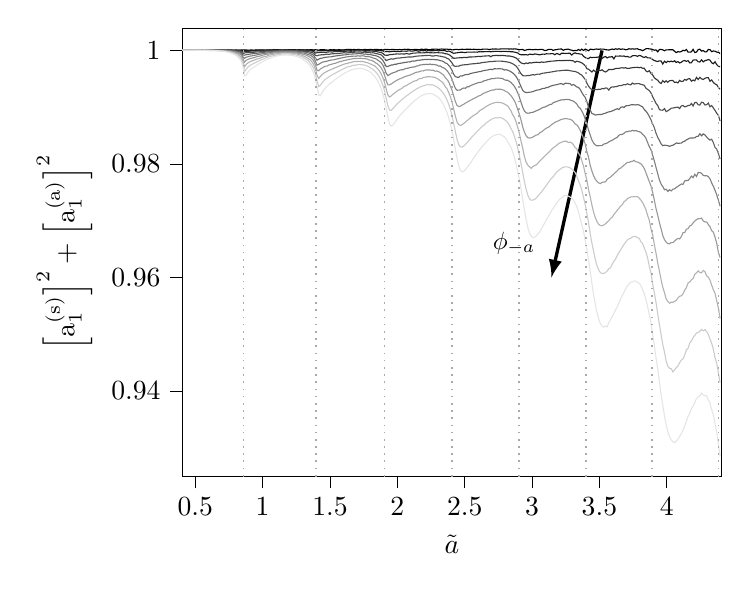
\begin{tikzpicture}

\definecolor{black25}{RGB}{25,25,25}
\definecolor{darkgray}{RGB}{169,169,169}
\definecolor{darkgray153}{RGB}{153,153,153}
\definecolor{darkgray176}{RGB}{176,176,176}
\definecolor{darkgray178}{RGB}{178,178,178}
\definecolor{darkslategray51}{RGB}{51,51,51}
\definecolor{darkslategray76}{RGB}{76,76,76}
\definecolor{dimgray102}{RGB}{102,102,102}
\definecolor{gainsboro229}{RGB}{229,229,229}
\definecolor{lightgray204}{RGB}{204,204,204}

\begin{axis}[
tick align=outside,
tick pos=left,
x grid style={darkgray176},
xlabel={\(\displaystyle \tilde{a}\)},
xmin=1, xmax=321,
xtick style={color=black},
xtick={8.8125,48.75,88.6875,128.625,168.5625,208.5,248.4375,288.375},
xticklabels={
  \(\displaystyle 0.5\),
  \(\displaystyle 1\),
  \(\displaystyle 1.5\),
  \(\displaystyle 2\),
  \(\displaystyle 2.5\),
  \(\displaystyle 3\),
  \(\displaystyle 3.5\),
  \(\displaystyle 4\)
},
y grid style={darkgray176},
ylabel={\(\displaystyle \Big[\mathrm{a}_1^{(\text{s})}\Big]^2+\Big[\mathrm{a}_1^{(\text{a})}\Big]^2\)},
ymin=0.924921672391509, ymax=1.00391663709987,
ytick style={color=black}
]
\draw[-latex,very thick,draw=black] (axis cs:250,1) -- (axis cs:220,0.96);
\addplot [black]
table {%
0 1.00006636262959
1 1.00005763051523
2 1.000057703946
3 1.00006044864142
4 1.00005787604676
5 1.00005797611006
6 1.00005808479128
7 1.00005820152389
8 1.00005832727063
9 1.00005846522253
10 1.0000586130052
11 1.00005877202897
12 1.00005894635015
13 1.00005912997859
14 1.00005932626032
15 1.0000595394729
16 1.00005976578295
17 1.00006000503969
18 1.00006025993993
19 1.0000605291046
20 1.0000608124279
21 1.00007057196262
22 1.00004904467763
23 1.00007135450139
24 1.00007177070861
25 1.00006240097976
26 1.0000627363479
27 1.00006306850758
28 1.00007353941458
29 1.00004609516445
30 1.00007440191715
31 1.00004214527282
32 1.00004583271438
33 1.00007540586732
34 1.0000676785184
35 1.00004897085546
36 1.00007424170824
37 1.00008597718007
38 1.00008882076773
39 1.00009012636972
40 1.00004863413332
41 1.00005628472667
42 1.00009395087359
43 1.00005887145359
44 1.00005375578436
45 1.00009845508488
46 1.00005672905998
47 1.00010175661121
48 1.00010343975098
49 1.00010511833047
50 1.00006285450661
51 1.00007097918798
52 1.00010994711013
53 1.00011144667844
54 1.00011287845566
55 1.00011424346992
56 1.00011553969638
57 1.00011677019933
58 1.00011793869094
59 1.00008019963575
60 1.00008102754868
61 1.00007477266361
62 1.0001220905885
63 1.00008313682732
64 1.00012390945709
65 1.00012476399357
66 1.00012558314445
67 1.00012636700969
68 1.00012711226918
69 1.00008577765681
70 1.00012847119968
71 1.00012907228942
72 1.00008611679984
73 1.00010506221726
74 1.00008579313205
75 1.00013067715198
76 1.00008478346559
77 1.0001305277576
78 1.00012962121494
79 1.00008597026767
80 1.00013257580669
81 1.00007960644881
82 1.0000615969099
83 1.00014232619709
84 1.00012580725101
85 1.00014559294385
86 1.00008717067652
87 1.0000684008629
88 1.00006998673868
89 1.00015315303042
90 1.00009406981846
91 1.00015755074491
92 1.00008703112988
93 1.00007922822748
94 1.00016468920629
95 1.00010439012259
96 1.0001065184598
97 1.00008726438332
98 1.00015508019267
99 1.00017685610324
100 1.00016939907707
101 1.00017159201404
102 1.00014648481008
103 1.00017573197854
104 1.00012139822742
105 1.0001794946742
106 1.00018122130071
107 1.00012526062262
108 1.00010324152959
109 1.00018571395309
110 1.0001672020581
111 1.00012841294042
112 1.00015947732103
113 1.0001788881636
114 1.00010449831362
115 1.00017003682906
116 1.00019096946404
117 1.00019070885523
118 1.0000996049641
119 1.00016517676183
120 1.00007895927341
121 1.00017132483517
122 1.00015508861522
123 1.00018393330387
124 1.00012784656066
125 1.00016269397988
126 1.00017665844959
127 1.00015451489356
128 1.0001565775296
129 1.00011865243378
130 1.00017344839017
131 1.00010631362597
132 1.00017864290291
133 1.00020830469742
134 1.00018435346185
135 1.0002145188268
136 1.00015557243688
137 1.00013898792293
138 1.00014187227995
139 1.00018704885437
140 1.00019015996431
141 1.00010963457818
142 1.00013539405652
143 1.00024088870132
144 1.00014032419805
145 1.00021810573561
146 1.00022073121685
147 1.000130272871
148 1.00011665624614
149 1.00021369193478
150 1.00021549213669
151 1.00023107300872
152 1.00023245724536
153 1.00015311547807
154 1.00023433876202
155 1.00024921462944
156 1.00021993345851
157 1.00021905963031
158 1.00023210611046
159 1.00018569850625
160 1.00020864428228
161 1.00010447001941
162 1.00011978656196
163 1.0001977845859
164 1.00020105708796
165 1.00012996004098
166 1.00018861100256
167 1.00020832263596
168 1.00019318664513
169 1.00019565008179
170 1.00021600968756
171 1.00020110682695
172 1.00020412546374
173 1.00019182325536
174 1.00021074168218
175 1.00018275421018
176 1.0001584637605
177 1.00019001828215
178 1.00014080313644
179 1.00021391003569
180 1.00023400251374
181 1.00023809006779
182 1.00024214749934
183 1.00013592688407
184 1.00021684727545
185 1.00025380361605
186 1.00024070900228
187 1.00026080130532
188 1.00022990348597
189 1.0002325709129
190 1.00026948305142
191 1.00027175905756
192 1.00027366060598
193 1.00027513974552
194 1.00027612590854
195 1.00024058612607
196 1.0002761085409
197 1.0002379563511
198 1.00027067094417
199 1.00026071037875
200 1.00018237060725
201 1.00014396299986
202 1.00015731701043
203 1.00016322936997
204 0.999993579224106
205 1.0000860577673
206 1.00017125454772
207 1.00017336900737
208 1.00015596294003
209 1.00012380780063
210 1.00016076891717
211 1.0001635419882
212 1.00013165201996
213 1.00016991353877
214 1.00019369097378
215 1.00014193020147
216 0.99999147197028
217 1.00002206751231
218 1.00015430565415
219 1.0001949151317
220 1.00019965089311
221 1.00000092802118
222 1.0001110777665
223 1.00014437165664
224 1.00021866896926
225 1.00024456789974
226 1.00024902820634
227 1.0000210397115
228 1.00016370726736
229 1.00020058534135
230 1.00024191157888
231 1.00011357459263
232 1.00004712509535
233 0.999933547584059
234 1.00001129462547
235 0.999966998042594
236 1.00017073620339
237 0.999999689548183
238 1.00023341003352
239 0.9999977107331
240 1.00023661707014
241 1.00011346179308
242 0.999946526222487
243 1.00023688591083
244 1.00018237351745
245 1.00013182252021
246 1.00024482691912
247 1.00024699734233
248 1.00019047734346
249 1.00025189814645
250 1.00022294158559
251 1.00022608340838
252 1.00014739422884
253 1.00010493452624
254 1.00006755684024
255 1.00015937869141
256 1.00024767913824
257 1.00014572887107
258 1.00029181796761
259 1.0002070313223
260 1.00030421313782
261 1.00019138655568
262 1.00025430373288
263 1.00023085595666
264 1.00011725705761
265 1.00016605055543
266 1.00030815846705
267 1.00022530900096
268 1.0002889892423
269 1.00023464250169
270 1.0002669799135
271 1.00030148243391
272 1.00014826516445
273 1.00010857678252
274 0.999958465290203
275 1.00010538575539
276 1.00030256924677
277 1.00032595688585
278 1.00027349148822
279 1.00024686053061
280 1.00016915132976
281 1.00003817792041
282 1.00010259540318
283 0.999758762753217
284 1.00017592958983
285 1.00017723419563
286 1.00010889182797
287 0.999946493128583
288 1.00011129995275
289 1.00011298397478
290 1.00011520389464
291 1.00011824237298
292 1.00012127671229
293 0.999855635605281
294 0.999623080593992
295 0.999797356770517
296 0.999725672958191
297 0.999805765890238
298 1.00003124338681
299 0.999940103249752
300 1.00016572492063
301 0.999708206912347
302 0.999695167310477
303 0.999759859451902
304 1.00019486469087
305 0.999629372866293
306 0.999714143512221
307 1.00014811919022
308 1.00022118811301
309 0.999882907545284
310 0.999979664468639
311 0.999746472517758
312 0.999767269483091
313 1.00017026074638
314 1.00013614381134
315 0.999791724691682
316 0.999903923879752
317 0.999863779356213
318 0.999702829463224
319 0.999671213074256
320 0.99946222101835
};
\addplot [black25]
table {%
0 1.00006326437676
1 1.00005024621788
2 1.00006647942666
3 1.00006656380826
4 1.00006665342258
5 1.00004637827345
6 1.00004449090588
7 1.00006696238074
8 1.00005815080909
9 1.00006719165237
10 1.000064189161
11 1.00006115002624
12 1.0000675584863
13 1.00004314881934
14 1.00006779774765
15 1.00004317703511
16 1.00004490957263
17 1.00006487550933
18 1.00004480137279
19 1.00005883546263
20 1.00004272223668
21 1.00005073040096
22 1.00006125703086
23 1.00006095739084
24 1.00006730695172
25 1.00005701097781
26 1.00004120429666
27 1.00003808791625
28 1.00005690177414
29 1.00005525055048
30 1.00005315871277
31 1.00005792995071
32 1.00005475128137
33 1.00002543604502
34 1.00002211460733
35 1.00003825874613
36 1.00002400989592
37 0.999967850376115
38 0.999993270886021
39 0.999971005406477
40 0.999984229488614
41 0.99997322825127
42 0.999978007232052
43 1.00001949567521
44 1.00002579682132
45 1.00003037344021
46 1.00003606446231
47 1.00004182870133
48 1.00004855178492
49 1.00005322865837
50 1.0000587039076
51 1.00006392383945
52 1.00003890200256
53 1.0000734186647
54 1.00004743345101
55 1.0000511187222
56 1.00008487781465
57 1.0000879268899
58 1.00009059611882
59 1.00008109882062
60 1.00006369659363
61 1.00006509313535
62 1.00006613161656
63 1.00008647722808
64 1.00005902164765
65 1.00009933826212
66 1.00009916373448
67 1.00005353105489
68 1.00009760440594
69 1.00003134559046
70 1.00009418234853
71 1.00009164283365
72 1.00008188846413
73 1.00007787827708
74 1.0000442157115
75 1.00007383608399
76 1.00005259846938
77 1.00001049160283
78 1.00004295057595
79 0.999989414564777
80 0.999906428743849
81 0.999909828730634
82 0.999969044948784
83 0.999935363627039
84 0.999981129193402
85 0.999977036060047
86 0.99999111803856
87 0.99997801825051
88 0.999941308664935
89 0.999998558115313
90 1.00001395361839
91 0.99995896150287
92 1.00000828020339
93 1.00003384157345
94 1.00004069501877
95 0.999984875914981
96 1.00005426188592
97 1.00004154812895
98 1.00005743406267
99 1.0000730223881
100 1.00005896870448
101 1.00001880493511
102 1.0000783285054
103 1.00002652755273
104 1.00008562524412
105 1.00008833352333
106 1.00008011694841
107 1.00009167245672
108 1.00009221917598
109 1.00003355590789
110 1.00003190131768
111 1.00001677817847
112 1.00002561606778
113 1.00007054596415
114 1.00004587609452
115 1.00004821685686
116 1.00002928177976
117 1.00003711106812
118 1.00003263480454
119 0.999941664971988
120 0.99994282711229
121 0.99976986516638
122 0.999819724610734
123 0.999808268544996
124 0.999751179975898
125 0.999807289700897
126 0.99983141601178
127 0.999870108357049
128 0.999799500332112
129 0.999848121291936
130 0.999784721632331
131 0.999860819915197
132 0.999889441167156
133 0.999875183472132
134 0.999863712679309
135 0.999925526452259
136 0.999921165314223
137 0.999887829269483
138 0.999895959039462
139 0.999959073209063
140 0.999967137592372
141 0.9998652339703
142 0.999925976792484
143 0.999988780922374
144 0.999937947426357
145 1.00000003712559
146 0.999878995745374
147 1.00002131695919
148 0.999933276877333
149 0.999952517593087
150 0.999952017096728
151 1.00000998905555
152 1.00000706621966
153 0.999905249721437
154 0.999995898710648
155 0.999987047298003
156 0.999975264946697
157 0.99995937387356
158 0.999811027295617
159 0.999899822434519
160 0.999820188567839
161 0.999628584001136
162 0.999496834012057
163 0.999548095262496
164 0.999587761510692
165 0.99963919409544
166 0.999678951724869
167 0.999685470876259
168 0.99965906898782
169 0.999623021786948
170 0.99970464171473
171 0.999694076218363
172 0.999701768452834
173 0.999710070095651
174 0.999718950817423
175 0.999712734534359
176 0.999691706771177
177 0.999784864724347
178 0.999758863574041
179 0.999769385465753
180 0.999779853969614
181 0.99979011430884
182 0.99980000529801
183 0.999793045030712
184 0.999769409893216
185 0.999809359478707
186 0.999832715219294
187 0.999838375718852
188 0.999842701642065
189 0.999845527529719
190 0.999796063800553
191 0.99984591878921
192 0.99984302851823
193 0.999837687572153
194 0.999793979644559
195 0.999817646330891
196 0.999765042840071
197 0.999777628592087
198 0.999705470642254
199 0.999644465758332
200 0.999555792100685
201 0.999322351198908
202 0.999249157313382
203 0.999251918735766
204 0.999235544332806
205 0.999263305579588
206 0.999184623324971
207 0.999354663646224
208 0.999319149325174
209 0.99927111859741
210 0.999373390689369
211 0.999359756236759
212 0.999291734224334
213 0.999217172471048
214 0.999309656736817
215 0.999355199815758
216 0.999330864603643
217 0.999420369524682
218 0.999390423034414
219 0.999403039175949
220 0.999436516796204
221 0.999428516653354
222 0.999237154328745
223 0.999452938284123
224 0.999394461927069
225 0.999251617259561
226 0.999505079235297
227 0.999512929217198
228 0.999459564469607
229 0.999482646289797
230 0.999503378404107
231 0.999502626759066
232 0.999192456094535
233 0.999452356207976
234 0.999577823006622
235 0.999442594753546
236 0.99943687315778
237 0.99935880804276
238 0.999339414511363
239 0.998972443960799
240 0.998775499135135
241 0.998588341453295
242 0.998564424495041
243 0.998817831323828
244 0.998732308167778
245 0.998783937620198
246 0.998789391631842
247 0.998794015875111
248 0.998851349800621
249 0.998757667294573
250 0.998576764987738
251 0.998814862040931
252 0.998936643700867
253 0.998676779805542
254 0.998842541573432
255 0.998853935152117
256 0.998921891558942
257 0.998523964264388
258 0.999012262588317
259 0.998995087274592
260 0.999011089376487
261 0.999027215808588
262 0.998985003558457
263 0.999029848269771
264 0.998895985828581
265 0.998952705241655
266 0.998817058001786
267 0.998826044238248
268 0.999059418977776
269 0.999095539119066
270 0.999067694744451
271 0.998965591832427
272 0.999123031312892
273 0.999050926829009
274 0.998867677652338
275 0.998770188224763
276 0.998910729038196
277 0.998697034610681
278 0.998696346432814
279 0.998632529600234
280 0.998387370661683
281 0.998226982343721
282 0.998122755043796
283 0.998047190083105
284 0.998172756334643
285 0.998138678399037
286 0.997603408666526
287 0.998104738392223
288 0.997860529147416
289 0.998108735266721
290 0.997996371953188
291 0.998118300967182
292 0.998008992555154
293 0.998171359007124
294 0.997877597822545
295 0.998041290135797
296 0.997785628519878
297 0.997918416206403
298 0.998144842200239
299 0.998227291368985
300 0.99807481754295
301 0.998201542106352
302 0.997803746314938
303 0.997838568429497
304 0.998287998446038
305 0.998340056005082
306 0.998320293159466
307 0.998000094798272
308 0.997967086097697
309 0.998349405982262
310 0.997985512403383
311 0.998203870710683
312 0.998275540038223
313 0.998398651404503
314 0.998293205161295
315 0.997833923394662
316 0.99764946485045
317 0.998011528771972
318 0.997501303668128
319 0.997233448906291
320 0.997119775846474
};
\addplot [darkslategray51]
table {%
0 1.00005013110666
1 1.00002939969867
2 1.0000602256284
3 1.00006645519491
4 1.00006344005027
5 1.00006039134889
6 1.00006665117642
7 1.00006361066225
8 1.00006676095089
9 1.00006680700695
10 1.00006683778756
11 1.0000527530662
12 1.00006684006951
13 1.00004227512688
14 1.00006355399559
15 1.00005745562657
16 1.00006320039803
17 1.0000296529472
18 1.00006574749292
19 1.00005593151947
20 1.00006134277165
21 1.00004897454663
22 1.00006271620792
23 1.0000613738193
24 1.00004193678421
25 1.0000478013943
26 1.00000210158549
27 1.00000981360237
28 1.00004058738392
29 1.00003242262342
30 1.00003654752528
31 1.00002159909319
32 0.999990508945424
33 1.0000080311162
34 0.999989281141617
35 0.999968734549546
36 0.999934745186431
37 0.999727467818457
38 0.999819548783906
39 0.999840266157167
40 0.999817187402792
41 0.999865962377498
42 0.999876469551857
43 0.999888228895463
44 0.99987123733461
45 0.999912951963153
46 0.999925769676751
47 0.999938691905054
48 0.999951526831088
49 0.999964081380551
50 0.999976178356359
51 0.99998765833699
52 0.99999839158343
53 1.00000828814527
54 1.00001728814795
55 1.00001960361639
56 1.00003248318782
57 1.00003867239018
58 1.00004393676386
59 1.00003651250974
60 1.00005177323744
61 1.00005437709549
62 1.00005610972904
63 1.00005698378302
64 1.00005697085088
65 1.0000560458479
66 1.00005416671094
67 1.00005127420467
68 1.00001422123399
69 1.00004209597872
70 1.00003557491727
71 1.00002756809778
72 1.00001785940759
73 0.999999547847424
74 0.999992174291331
75 0.999975257620559
76 0.999954473459635
77 0.999927685890496
78 0.999889125687837
79 0.999812769178756
80 0.999525907941926
81 0.99960365636612
82 0.999625467475289
83 0.99967158098369
84 0.999677278457757
85 0.999698859592343
86 0.999649155007967
87 0.999722737338735
88 0.99973513321956
89 0.999757279029035
90 0.999703921587591
91 0.999784834582905
92 0.99978990093353
93 0.999778709763553
94 0.999828555738053
95 0.999793197373752
96 0.999847809193765
97 0.999807831173686
98 0.999833347513602
99 0.999896231013201
100 0.999887828166686
101 0.999841132631933
102 0.999889149360505
103 0.999856228071483
104 0.999939354746634
105 0.999933575151026
106 0.999936110748723
107 0.99993685694538
108 0.999935700746587
109 0.999862033261446
110 0.999856034454516
111 0.99991938854142
112 0.999879662318206
113 0.999884878955807
114 0.999879115342148
115 0.999811428786198
116 0.999832808661201
117 0.999736871772217
118 0.999692059712318
119 0.999624290255605
120 0.999491281098101
121 0.999192829599315
122 0.99915021214722
123 0.999146568579242
124 0.999265700653004
125 0.999270157089499
126 0.999305435217735
127 0.999353207769013
128 0.999379238553811
129 0.999393281647069
130 0.999351880104333
131 0.999410700779376
132 0.999373570075874
133 0.999380849697715
134 0.999460267412621
135 0.999384891096411
136 0.999378172221598
137 0.999459520609622
138 0.999531749417942
139 0.999525148095065
140 0.999578768893041
141 0.99958173816759
142 0.99959635213736
143 0.999573355638144
144 0.999584603558973
145 0.999593918604712
146 0.999637960993173
147 0.99964296837611
148 0.999587076443949
149 0.999586137125084
150 0.999582020069472
151 0.999595747965581
152 0.999623051223582
153 0.999593449737074
154 0.999572919179712
155 0.999560803576851
156 0.999541097234732
157 0.999418735985756
158 0.999405229628219
159 0.999286386430018
160 0.99912417145307
161 0.99885595211384
162 0.998611773957631
163 0.998641183080721
164 0.998675062689914
165 0.998695041826537
166 0.99873448132542
167 0.998697376604734
168 0.998788426323061
169 0.998756765198178
170 0.998746041979925
171 0.998838089319137
172 0.998838191964588
173 0.998857036817847
174 0.998876919258106
175 0.99888218570782
176 0.998937559172481
177 0.998959958140903
178 0.998917296010063
179 0.998986680897911
180 0.999008882392876
181 0.999030404672416
182 0.999034694426014
183 0.99906991412706
184 0.998907299609386
185 0.999069031424657
186 0.999098081395134
187 0.999124134771999
188 0.999113439934775
189 0.999098464061553
190 0.999113434632959
191 0.999123557385951
192 0.999093860285598
193 0.999057277774569
194 0.999013975741587
195 0.999030182049611
196 0.998964400756083
197 0.998899046426482
198 0.998806707665491
199 0.998666944955455
200 0.99841858499669
201 0.998061742032933
202 0.997805656867831
203 0.997690294044198
204 0.997653006534282
205 0.997806185593219
206 0.99768183957884
207 0.997852918065859
208 0.997776694685615
209 0.997868421392185
210 0.99788605427133
211 0.997925362939914
212 0.997903083934357
213 0.997869511789133
214 0.997968440136244
215 0.997916045882784
216 0.997941460203688
217 0.997968014670998
218 0.998051497846547
219 0.998059105531154
220 0.998129855486279
221 0.998114803292007
222 0.998162363426518
223 0.998187759084574
224 0.998211183031443
225 0.998232068716976
226 0.998191285612534
227 0.998242445403338
228 0.998214301845012
229 0.998256461463938
230 0.998216914071113
231 0.998268881007196
232 0.998192167294071
233 0.998166414911123
234 0.997918437647415
235 0.998097266828485
236 0.998026033062515
237 0.997946665171769
238 0.997804471610528
239 0.997592558770117
240 0.997325263827107
241 0.996797752810349
242 0.996675878513746
243 0.996449142793455
244 0.996205153799383
245 0.996544667490116
246 0.996248295096321
247 0.996420389599296
248 0.996559919634223
249 0.996450821334422
250 0.996592911637258
251 0.996349415359816
252 0.996205581578688
253 0.996366660634047
254 0.996655495967751
255 0.996629556328718
256 0.996637070549418
257 0.996692416734577
258 0.996809835576283
259 0.99684511608975
260 0.996852661051628
261 0.996916477008576
262 0.996951156598053
263 0.996898965374637
264 0.996957144182978
265 0.996827860003584
266 0.996850852540077
267 0.996907551299008
268 0.996963730885174
269 0.996994865123912
270 0.997017524031177
271 0.997034617846242
272 0.996958366256489
273 0.997037252933892
274 0.99686703091364
275 0.996876091251808
276 0.996398114880578
277 0.99623481880783
278 0.996435604150515
279 0.995963605581347
280 0.995673059524655
281 0.995192276742599
282 0.994932213871658
283 0.994762647008948
284 0.994373558363078
285 0.994174042385729
286 0.994685267671972
287 0.994392205997208
288 0.994656830631737
289 0.994387477999444
290 0.994679306290332
291 0.994697195105808
292 0.994718503918205
293 0.994351660632104
294 0.994428890215048
295 0.994279995075787
296 0.99472491890298
297 0.994533378597406
298 0.994573666391418
299 0.994904003901462
300 0.994755575243893
301 0.994992601346829
302 0.995036186235624
303 0.994576693556564
304 0.994794449289277
305 0.994643358026934
306 0.995247803917728
307 0.994878578542651
308 0.995252562446932
309 0.994989454105468
310 0.994890883785372
311 0.995091795087093
312 0.995200399712318
313 0.995219869135997
314 0.994570229182251
315 0.994798694489663
316 0.994366687134763
317 0.994095107444607
318 0.99396767805245
319 0.993486185534497
320 0.993151638834174
};
\addplot [darkslategray76]
table {%
0 1.00005737053799
1 1.00005740346497
2 1.00005007671361
3 1.00006628758805
4 1.00005009113152
5 1.00005008114726
6 1.00005745949199
7 1.00005237967796
8 1.00006319100574
9 1.00005728948372
10 1.00004969074085
11 1.00005189036007
12 1.00005947695267
13 1.00006549927654
14 1.00006513370962
15 1.00006147714541
16 1.00004722989869
17 1.00004636565104
18 1.00004775688589
19 1.00004643513712
20 1.00004480080795
21 1.00004278808765
22 1.00005190292936
23 1.00005229313567
24 1.00004869940937
25 1.00002638770797
26 1.00003544403465
27 1.00002227339078
28 1.00002413594709
29 0.999998167247489
30 1.00000207574256
31 0.999983526477868
32 0.999965133032162
33 0.999925986593839
34 0.999916843671605
35 0.999876527057014
36 0.999804550103937
37 0.999413694683204
38 0.999550146914993
39 0.999601800243918
40 0.999624587244969
41 0.999653185669036
42 0.999664046103234
43 0.999668016105605
44 0.999698833807541
45 0.99974256242866
46 0.999736619354919
47 0.999759974955696
48 0.999812589801066
49 0.999835238926664
50 0.999851370952154
51 0.999877599516155
52 0.99989679989945
53 0.999870109504952
54 0.999892630008356
55 0.999938893387653
56 0.999957131484982
57 0.999967880734722
58 0.999976913687649
59 0.999972493126439
60 0.999989967434922
61 0.999994041820274
62 0.99998450639067
63 0.999985255069945
64 0.999990438860145
65 0.999995016542044
66 0.999977263164243
67 0.999983353673094
68 0.999942023722815
69 0.999964401360027
70 0.999944863066059
71 0.999935251805477
72 0.99991598410067
73 0.999858075479284
74 0.999865279705856
75 0.999831936866186
76 0.999784037963167
77 0.999701399386032
78 0.999663757364359
79 0.999491994392258
80 0.999155809453462
81 0.999063902450501
82 0.999173666777671
83 0.999203895550409
84 0.999262740008444
85 0.999233310117849
86 0.999322745752453
87 0.999346119492115
88 0.999303501255338
89 0.999375393935899
90 0.999409493373093
91 0.999425678271252
92 0.999451682570024
93 0.999429029655058
94 0.999460974543261
95 0.999521925177316
96 0.999555318415568
97 0.999598694580112
98 0.999552123748971
99 0.999573025495986
100 0.999662315120222
101 0.999608782720699
102 0.999623164365746
103 0.999678127175169
104 0.999706073346172
105 0.999712489058481
106 0.999725861573262
107 0.999715628768537
108 0.999647863963562
109 0.99970439945755
110 0.999682182791385
111 0.999617399047637
112 0.999655300268493
113 0.999561421125655
114 0.999595106685082
115 0.999542891188738
116 0.999440691552877
117 0.999398974938515
118 0.999304222331716
119 0.999228712695392
120 0.998949840864412
121 0.998579487988776
122 0.998223202885877
123 0.998341020291886
124 0.998429760720499
125 0.998530961835485
126 0.998471432305807
127 0.998533020462355
128 0.998635009301391
129 0.998663584349812
130 0.998646404107573
131 0.998721250353052
132 0.998738986386106
133 0.998769868798763
134 0.9988139779268
135 0.998846384818033
136 0.998853919935606
137 0.998844934462877
138 0.998876740552445
139 0.998949569728505
140 0.998992201367983
141 0.99902011266878
142 0.99904568978821
143 0.999055312403004
144 0.999074797993235
145 0.999103965503308
146 0.999115767179189
147 0.99913641743741
148 0.99912528849843
149 0.999020877716307
150 0.999010839106995
151 0.999082925540276
152 0.999087399527696
153 0.999027496434891
154 0.998985759311759
155 0.998932239699727
156 0.998863860645178
157 0.998804701005897
158 0.998608722708809
159 0.998504825212013
160 0.998180767330956
161 0.997823433779975
162 0.997316611264565
163 0.99718591101995
164 0.99724545444485
165 0.997223223593287
166 0.997377215636471
167 0.997423878411138
168 0.997463656767167
169 0.997499958049252
170 0.997486937960762
171 0.997569957640315
172 0.997605766642891
173 0.997642791332399
174 0.997663261233003
175 0.997671565494227
176 0.997743423344964
177 0.99773828471528
178 0.997794504239852
179 0.997867476043683
180 0.997907812560034
181 0.99793059382019
182 0.997967113323243
183 0.998016959857283
184 0.998047103075789
185 0.998039931619876
186 0.998093785647015
187 0.998108841573228
188 0.998117331010538
189 0.998118418899619
190 0.998111164809481
191 0.998094482412669
192 0.998049875191737
193 0.998009904618685
194 0.997955253911299
195 0.997900268733139
196 0.997787229072955
197 0.997660903638131
198 0.99747168427375
199 0.997250340463943
200 0.996883627239916
201 0.996344321259307
202 0.995881336444295
203 0.995574897381913
204 0.995510291672534
205 0.995538140409681
206 0.995584765434877
207 0.99559118545646
208 0.995673944651148
209 0.995735206912117
210 0.995680178475129
211 0.995774301287631
212 0.995837275622517
213 0.99580550843348
214 0.995927248400416
215 0.995996602096135
216 0.996025639091444
217 0.996077347311383
218 0.996130066341967
219 0.996161299335257
220 0.99621387345988
221 0.996265195773874
222 0.996314393713526
223 0.996382797108507
224 0.996402499113933
225 0.996418287158961
226 0.996469989347925
227 0.996493220052721
228 0.996507819202366
229 0.996512448022479
230 0.996505581703162
231 0.996425407344584
232 0.996389454983546
233 0.996318342460766
234 0.99632048233713
235 0.99617581834972
236 0.99605754680341
237 0.99579824373495
238 0.995647836851736
239 0.995266158953664
240 0.994904031138447
241 0.994224175023245
242 0.993704495443831
243 0.993314127675708
244 0.993107724159558
245 0.993070206765068
246 0.99309293991086
247 0.993088349793201
248 0.993170941027736
249 0.993131391356407
250 0.993303546500411
251 0.993234797233288
252 0.99339269382321
253 0.993357341288275
254 0.993015690092942
255 0.993443577392955
256 0.993587041639625
257 0.993546187158285
258 0.993635319643295
259 0.993656061188416
260 0.993797166171745
261 0.993789883959918
262 0.993878003237137
263 0.993989661301342
264 0.993949720582392
265 0.994125077392181
266 0.993980669460935
267 0.993947104610065
268 0.994249431504604
269 0.994076645419313
270 0.994135369703004
271 0.994160141597262
272 0.994140590268297
273 0.994033109301515
274 0.993955657361352
275 0.993873423557375
276 0.993356620307031
277 0.993143732780793
278 0.992932389074686
279 0.992507084398071
280 0.991841028937279
281 0.991286105925847
282 0.990664049509233
283 0.990299561207542
284 0.989586253631845
285 0.989480338488931
286 0.98947242918272
287 0.989748761546951
288 0.989216307101899
289 0.98938089315376
290 0.989573441839141
291 0.989830908346142
292 0.989841768004026
293 0.989931695650826
294 0.989959622783785
295 0.990028373868615
296 0.989758319683434
297 0.990218426322564
298 0.990301668233415
299 0.990062508329136
300 0.990147526540413
301 0.990307166425457
302 0.990313675187447
303 0.990651400428533
304 0.990208767305165
305 0.990822841444537
306 0.99084352778166
307 0.990422621277122
308 0.990379176011432
309 0.990882775258796
310 0.990808409216321
311 0.990393384897154
312 0.990442842313943
313 0.990741447516798
314 0.990078317109563
315 0.99029264408582
316 0.989860180246682
317 0.989440078334256
318 0.988927701959685
319 0.988566061752641
320 0.987572096969079
};
\addplot [dimgray102]
table {%
0 1.00005722715315
1 1.00006604526518
2 1.00005722614829
3 1.00005720781078
4 1.00005215532043
5 1.00005208565448
6 1.0000664415155
7 1.00006633698758
8 1.00006254107432
9 1.00005649716212
10 1.00005111497164
11 1.00005071150451
12 1.00006119674338
13 1.0000605926004
14 1.00004875724229
15 1.00006260457698
16 1.00006143343603
17 1.00005021396818
18 1.00004311541147
19 1.00005216373957
20 1.00004941605356
21 1.00003990174547
22 1.00004193110776
23 1.00004081132771
24 1.000034124598
25 1.00001691934152
26 1.00000772809905
27 0.999988234713787
28 0.999985949192621
29 0.999976522050488
30 0.999946033621705
31 0.999931772064911
32 0.999893938885169
33 0.999859763787032
34 0.999803816613941
35 0.999743882572647
36 0.99962820486481
37 0.999198039041642
38 0.999161618386025
39 0.999272452258958
40 0.999286780806559
41 0.999356347859118
42 0.999388790260776
43 0.999442063507703
44 0.999441376119369
45 0.999504080395891
46 0.999523617711667
47 0.999553797411965
48 0.999611768176253
49 0.999652798598771
50 0.999687499683057
51 0.999731606134489
52 0.99972820430869
53 0.99976012421125
54 0.999809667899144
55 0.999837861806429
56 0.999857510805365
57 0.999843809125377
58 0.999888402891278
59 0.99989974489236
60 0.99989657960766
61 0.99991446521637
62 0.999900746806903
63 0.999906619177806
64 0.999873034551346
65 0.999912091522465
66 0.999892155617567
67 0.999875954211429
68 0.999879637183858
69 0.999855487560207
70 0.999833434411293
71 0.99980668745498
72 0.999781056250459
73 0.999707938926085
74 0.999696694771658
75 0.999642348175406
76 0.999553136411023
77 0.999478442396465
78 0.999326584919256
79 0.999147771212106
80 0.998657283605381
81 0.998298129535198
82 0.998453438605213
83 0.998613576210116
84 0.998644890537212
85 0.998734470255628
86 0.998787308677905
87 0.998828194594091
88 0.998859165200969
89 0.998860331499775
90 0.998923227984804
91 0.998982227891176
92 0.999033819485267
93 0.999067015434535
94 0.999091698335399
95 0.999141341816846
96 0.99919117726345
97 0.999211883418417
98 0.999225122948484
99 0.999299640553597
100 0.999339767476604
101 0.999347098871545
102 0.999370003302688
103 0.999398632286238
104 0.999394186939991
105 0.999432215695053
106 0.999436493480864
107 0.99942512247593
108 0.999407676655082
109 0.999340172226684
110 0.999373882365617
111 0.999291179719462
112 0.99926793040359
113 0.999264802491987
114 0.999158882103052
115 0.99913953224758
116 0.999054091602556
117 0.998946651449156
118 0.998796618671478
119 0.998590602127807
120 0.998251002733794
121 0.99776521887587
122 0.997173507667684
123 0.99716506870577
124 0.99731354800394
125 0.997427280596678
126 0.997447087116213
127 0.9975634021737
128 0.997568241568787
129 0.997684058071183
130 0.997722571368032
131 0.997772962662373
132 0.997823934678306
133 0.997888065680922
134 0.997915966947462
135 0.997981705140163
136 0.997972224620671
137 0.998100630675108
138 0.998140014866348
139 0.998126296732293
140 0.998213912763751
141 0.998295334555306
142 0.998276702477572
143 0.998345929161114
144 0.998376454181239
145 0.998427382879342
146 0.99839534144587
147 0.998428794526758
148 0.998407157111523
149 0.998411832908465
150 0.998420322302973
151 0.998366440006269
152 0.998365810424967
153 0.99831158557172
154 0.998212781853396
155 0.99815128071018
156 0.998037326028567
157 0.997795000786597
158 0.997701372331215
159 0.997400296598565
160 0.997030506701772
161 0.99650065289129
162 0.995816478611957
163 0.995393428681441
164 0.995288227467901
165 0.995274169768537
166 0.99552616341259
167 0.995502292634207
168 0.99562883862328
169 0.995746067762711
170 0.995737570459145
171 0.99580146594085
172 0.99594050989648
173 0.99600560233788
174 0.99607192765696
175 0.996139553245635
176 0.996174637358235
177 0.996259236953306
178 0.996268783075824
179 0.996396110121495
180 0.996462192449754
181 0.996509445962101
182 0.996552385676438
183 0.996622842608565
184 0.996687124653364
185 0.996607376720789
186 0.996779451425309
187 0.99676659068601
188 0.996761362310224
189 0.996794251684996
190 0.996762850563053
191 0.996732480991841
192 0.996545370159663
193 0.996615471566353
194 0.996522561281712
195 0.996400656053163
196 0.996242659634568
197 0.996037981325766
198 0.995770168721687
199 0.995413812749857
200 0.994914975098801
201 0.99428259596538
202 0.99357257781962
203 0.992964806510632
204 0.992677510317769
205 0.992586037207664
206 0.992579130590648
207 0.992644962563832
208 0.992670963133628
209 0.992760802387379
210 0.99286987721333
211 0.992986211153525
212 0.993042929469011
213 0.993085935310601
214 0.993226196236367
215 0.993311171726893
216 0.993306751884588
217 0.993487301399767
218 0.99346870494589
219 0.993666660425755
220 0.993754917362071
221 0.99386215659869
222 0.993899928674001
223 0.993975662709052
224 0.994044137295934
225 0.994126090594958
226 0.994152460870036
227 0.993978257849316
228 0.994210199528099
229 0.994214921545759
230 0.994178760788568
231 0.99416360073194
232 0.993866667602817
233 0.99400916320753
234 0.993803960491609
235 0.993570769853842
236 0.993489531150678
237 0.993158782579404
238 0.992601208570073
239 0.992099236752548
240 0.991735912285167
241 0.990977605180531
242 0.989978524918202
243 0.989478360951301
244 0.988867269185347
245 0.988796412285544
246 0.988607770244101
247 0.988678123793246
248 0.988706115485157
249 0.988711126328801
250 0.988755090732855
251 0.988875977090865
252 0.98893845309206
253 0.989078153325558
254 0.989176439066367
255 0.989231904793198
256 0.989340476811695
257 0.989452831413776
258 0.989616907926046
259 0.989733063020558
260 0.9895844016547
261 0.989961687211016
262 0.990070293778986
263 0.989941807454212
264 0.990238147942162
265 0.99027198631644
266 0.990296668029727
267 0.990414143565943
268 0.990445058159655
269 0.990429040386134
270 0.990387789065205
271 0.990466726074405
272 0.990380583734056
273 0.990221839394833
274 0.990073298112454
275 0.989604301980568
276 0.989308975426361
277 0.98890932238751
278 0.988371016692139
279 0.987782427599503
280 0.987056110969424
281 0.986391529771025
282 0.985430478315117
283 0.984710564472739
284 0.984133923209304
285 0.983534725448025
286 0.983212612064344
287 0.983323769500346
288 0.983266271926769
289 0.983232705149444
290 0.983084155386534
291 0.983243529461056
292 0.983300988097139
293 0.98346809884797
294 0.983702908482908
295 0.983628619459889
296 0.983658194124847
297 0.983670436211144
298 0.983907359620605
299 0.984009475810628
300 0.984251988902913
301 0.984397441376566
302 0.984558460505819
303 0.984572990767617
304 0.984579911852084
305 0.984594435000533
306 0.9848585744248
307 0.984874809324024
308 0.985311867450889
309 0.984964593947804
310 0.985288973917525
311 0.985125744076681
312 0.984758557566559
313 0.984456653669924
314 0.984203184810656
315 0.984360472253985
316 0.983755385536224
317 0.982907453012847
318 0.98260026844257
319 0.981832310935337
320 0.980863562343536
};
\addplot [gray]
table {%
0 1.00005203241292
1 1.00005699681299
2 1.00004959378816
3 1.00005687220345
4 1.0000656204446
5 1.00004924417412
6 1.00004903783401
7 1.00005114216624
8 1.00005586715244
9 1.00005545422468
10 1.00004745910381
11 1.00004678040805
12 1.00002797228724
13 1.00006201961529
14 1.00005707931956
15 1.00003972188665
16 1.00004003740907
17 1.0000401008583
18 1.00001630877526
19 1.00003365861351
20 1.00002935361599
21 1.00002945751317
22 0.999996305456752
23 1.00002557290115
24 1.0000060749647
25 0.999994709795204
26 0.999972701040502
27 0.999955836352772
28 0.99995438446843
29 0.999929679127581
30 0.99989888566947
31 0.99984267226839
32 0.99981700776608
33 0.999760059170217
34 0.999675031407702
35 0.999556704479637
36 0.999392759600325
37 0.998896758891534
38 0.998627902696921
39 0.998812642072419
40 0.998889920011687
41 0.998999802782059
42 0.999029533328981
43 0.999085616019469
44 0.999145533503849
45 0.999197294375042
46 0.999266822210063
47 0.999302073019599
48 0.99939504061758
49 0.999448646229478
50 0.999458287687003
51 0.999531140855658
52 0.999586630540352
53 0.999627751275863
54 0.999671535581321
55 0.999697737351976
56 0.999701851150986
57 0.999726257337309
58 0.999777218952397
59 0.999794626706356
60 0.999806059783077
61 0.999787957725345
62 0.999813313988452
63 0.999793028077235
64 0.999816792577064
65 0.999765425041968
66 0.999791578782305
67 0.999775165438076
68 0.999759947682692
69 0.999714893788973
70 0.999650348202486
71 0.999641161245226
72 0.999577091458396
73 0.999528869759582
74 0.999485387152944
75 0.999348037362606
76 0.999261566570297
77 0.999159642523032
78 0.998980663728053
79 0.998709189421685
80 0.998101027324879
81 0.997421658965668
82 0.9975521364214
83 0.997743069345904
84 0.997916742174208
85 0.997999194716497
86 0.998051321371483
87 0.998117635187315
88 0.998210734217603
89 0.998282666986853
90 0.998336333700517
91 0.998351417343976
92 0.99843318217962
93 0.998519094756527
94 0.998559701422817
95 0.998661579344178
96 0.99871186366958
97 0.99876889462093
98 0.998843313837917
99 0.998881517151721
100 0.998916432617775
101 0.998965514270776
102 0.998980629192017
103 0.999007658807558
104 0.998979176359973
105 0.99905963998641
106 0.99901491007427
107 0.99902682825236
108 0.999061122916532
109 0.999019638161368
110 0.998895131305318
111 0.99894616704509
112 0.998891425423358
113 0.998822650379997
114 0.998694687645341
115 0.998605866973439
116 0.998504297099653
117 0.998299046884646
118 0.998071229037193
119 0.997846575198695
120 0.997427305918997
121 0.996797597320521
122 0.995985749370923
123 0.995569678413185
124 0.995757700796741
125 0.995940429445213
126 0.996051086427424
127 0.996165969483192
128 0.996263285559401
129 0.996430948856987
130 0.996514235654213
131 0.99659548616348
132 0.996595016408884
133 0.996757338889568
134 0.99683883730632
135 0.996873876312122
136 0.996976788749998
137 0.997034932627363
138 0.997084408966609
139 0.99709892154332
140 0.997259215383719
141 0.997279941638944
142 0.997433888822772
143 0.997461069507703
144 0.997519153396658
145 0.997530261517908
146 0.997567174280707
147 0.997519438738203
148 0.997610015874053
149 0.997508390422696
150 0.997544248133912
151 0.997488734866798
152 0.997438502554472
153 0.997232855054628
154 0.997275994840311
155 0.997054511164502
156 0.996939907396636
157 0.996752246815402
158 0.996460539755273
159 0.996069037584898
160 0.995605115054431
161 0.994947033302965
162 0.994067160097867
163 0.993334567701543
164 0.992985599730883
165 0.993010590665467
166 0.993044518201652
167 0.993271304032658
168 0.993383888910462
169 0.993335498742549
170 0.993615034097475
171 0.993594104938132
172 0.993811244168689
173 0.993916886110445
174 0.994040811814541
175 0.994147848442433
176 0.994255411562316
177 0.994362883210991
178 0.994379084150511
179 0.994471551591107
180 0.994656336517988
181 0.994705301566727
182 0.994826005707311
183 0.994907623421386
184 0.994979651095845
185 0.99505664496942
186 0.995028981669828
187 0.995121051372501
188 0.995137227435255
189 0.995134589708878
190 0.995077928963705
191 0.995063324064646
192 0.994850984235365
193 0.994754455348378
194 0.994742921582981
195 0.994559830652063
196 0.994363365146504
197 0.994027235391063
198 0.993685576793007
199 0.993159771691853
200 0.992534557233514
201 0.991748872752225
202 0.990836080535021
203 0.989952417534914
204 0.989319365174033
205 0.989012849139365
206 0.988938297914338
207 0.988981238383655
208 0.98907424421235
209 0.989099398885275
210 0.989234573766893
211 0.98935927609458
212 0.989487160333306
213 0.989618132882503
214 0.989827267336697
215 0.989964608978135
216 0.990013257490331
217 0.990169231171685
218 0.990294895336178
219 0.990485334395834
220 0.990502760710701
221 0.99079672164232
222 0.990900193714589
223 0.991016232415464
224 0.991120651321475
225 0.991210952778488
226 0.991306902377686
227 0.991299215205341
228 0.991330510013014
229 0.991375812010282
230 0.991352252186324
231 0.991295270116403
232 0.991159567429527
233 0.991060879601648
234 0.99084859118176
235 0.990578821794066
236 0.990058632135202
237 0.989847497659222
238 0.989333891582939
239 0.988737854448036
240 0.987915654496646
241 0.986999147539768
242 0.985958187182398
243 0.985067242906574
244 0.984216696984527
245 0.983680245714904
246 0.98333963219443
247 0.983196202406193
248 0.983212852368883
249 0.983228337513748
250 0.983248676068013
251 0.98350176978349
252 0.983579718929455
253 0.983678256452505
254 0.983883628750974
255 0.984050848060957
256 0.984177128142611
257 0.984356754895994
258 0.98453947514312
259 0.984699746089986
260 0.985073976513748
261 0.985186980438754
262 0.98520621075301
263 0.985408013865128
264 0.985658868263096
265 0.985676754604688
266 0.985803670214841
267 0.98577256258055
268 0.98592829210539
269 0.985811024610766
270 0.985888092612669
271 0.985766296034488
272 0.98568326298351
273 0.985576085250345
274 0.985232553370945
275 0.984974045826204
276 0.984539312577045
277 0.983777786678633
278 0.983073262000827
279 0.982518671287632
280 0.981548478611643
281 0.980532681076332
282 0.979395475262562
283 0.978294191192395
284 0.977203626678753
285 0.976469825513971
286 0.976020747417748
287 0.975457795225895
288 0.975553248362204
289 0.975159549078352
290 0.975459390787276
291 0.975243668149772
292 0.975554021278351
293 0.975610790027512
294 0.975858315485266
295 0.976048944866765
296 0.976256503980805
297 0.976474581787275
298 0.976395607198857
299 0.97700453287775
300 0.977086083592824
301 0.977088056592989
302 0.977421562981894
303 0.977862540614081
304 0.977590691605769
305 0.978183288673274
306 0.977798424701392
307 0.978492665249345
308 0.978482731146962
309 0.97835719514122
310 0.977980182762109
311 0.977905458057643
312 0.977940409449549
313 0.977767408637476
314 0.977388832905514
315 0.976664965709548
316 0.976068129664456
317 0.975343813557878
318 0.974559387127826
319 0.973606127618392
320 0.972561313953603
};
\addplot [darkgray153]
table {%
0 1.00004722131509
1 1.00006602041603
2 1.0000659243445
3 1.00006579800644
4 1.00004886403975
5 1.0000464051993
6 1.00006456298977
7 1.00006417566126
8 1.00006368364914
9 1.00006306526378
10 1.00004585261305
11 1.00005232655422
12 1.00006153692646
13 1.00003979237514
14 1.00005735157821
15 1.00003557439385
16 1.00000511071474
17 1.0000004834306
18 0.999995982499492
19 1.00003619126609
20 1.00003013532008
21 1.00000644821578
22 1.00000767679326
23 1.00000303240635
24 0.999993838232109
25 0.999977933669388
26 0.999926133375513
27 0.999913876433518
28 0.999906637967937
29 0.999861107408478
30 0.999829503064802
31 0.999766429060898
32 0.999709056765948
33 0.999628706235567
34 0.999525263106573
35 0.999383306141526
36 0.999158135232755
37 0.998552185001923
38 0.997938986419327
39 0.998278442514953
40 0.998403531495018
41 0.99854239576054
42 0.998613642799968
43 0.998695596909348
44 0.998755195856806
45 0.998872474587109
46 0.998952164359669
47 0.998996913673307
48 0.999096579823737
49 0.99918391535831
50 0.99925569607954
51 0.999306115704314
52 0.999351148999273
53 0.999412448550778
54 0.999459872426105
55 0.999540801404764
56 0.999549373202574
57 0.999579127823051
58 0.999599970822699
59 0.999665662384125
60 0.999682760326268
61 0.999650625173319
62 0.999668249574955
63 0.999683100457071
64 0.999683385405007
65 0.99966742506884
66 0.999662058376257
67 0.999638801398489
68 0.99961578683764
69 0.999512543302025
70 0.999511632839426
71 0.999474287279339
72 0.999406211247
73 0.999289012495653
74 0.999226969851905
75 0.999108934954071
76 0.998962885021772
77 0.998780646748646
78 0.998534628387399
79 0.998159183605248
80 0.997513801025296
81 0.996488564970867
82 0.99642574397747
83 0.996742917343069
84 0.996904484525829
85 0.997096913433501
86 0.997222377278846
87 0.997250973191945
88 0.997440766805392
89 0.997505811246601
90 0.997605503906516
91 0.997706331244218
92 0.997739974902028
93 0.997871124513705
94 0.99798911038954
95 0.998047915003116
96 0.99813213741964
97 0.998212240194069
98 0.998295585113796
99 0.998333392992555
100 0.998427053230588
101 0.998473385989436
102 0.998528271265668
103 0.998585567317508
104 0.99858520980334
105 0.998602957059117
106 0.998593518636434
107 0.998624267888708
108 0.998556724086034
109 0.998567213834655
110 0.998522811608122
111 0.998473207484994
112 0.998290310188596
113 0.998287636372064
114 0.998167337056062
115 0.998000925964205
116 0.997748737974483
117 0.997604377410429
118 0.997300796988673
119 0.99694348782561
120 0.996411510356272
121 0.995662723042183
122 0.994671713487559
123 0.993941328404242
124 0.993946750409202
125 0.994096139285529
126 0.994317675547888
127 0.99450232031085
128 0.994693300944947
129 0.99485343928121
130 0.995006833842238
131 0.995106523578135
132 0.995227793134827
133 0.995372427546169
134 0.995467330240258
135 0.995564413133563
136 0.99565357815586
137 0.995796848484339
138 0.995872244389236
139 0.996063318466884
140 0.996164787370463
141 0.996200279387105
142 0.996318299463744
143 0.996406163888584
144 0.996387358660377
145 0.996532519046854
146 0.996568117404441
147 0.996561038206663
148 0.996551165720938
149 0.99651054599225
150 0.996506376965228
151 0.996324056999863
152 0.996383137702936
153 0.99626526937099
154 0.99611349384083
155 0.995893590488317
156 0.99568239939561
157 0.995227862365463
158 0.994918704071695
159 0.994495575057731
160 0.993759881306659
161 0.99301699418627
162 0.992007698761758
163 0.99100432551772
164 0.990330045605022
165 0.990116229590374
166 0.990183504604074
167 0.990382467734005
168 0.990519149923446
169 0.99073223490176
170 0.990888650322308
171 0.991073330164793
172 0.991219389716937
173 0.99138081238654
174 0.991541387243475
175 0.99168626746582
176 0.991845776795593
177 0.99200393893239
178 0.992080609557468
179 0.992327050907386
180 0.992473244642651
181 0.992596036110157
182 0.992724917303272
183 0.992841985669202
184 0.992944988574591
185 0.993031618080652
186 0.993019958795266
187 0.993181359646222
188 0.993168608056859
189 0.993164408704378
190 0.993166276447002
191 0.993062496787685
192 0.992956972268504
193 0.992761179109083
194 0.992648040658888
195 0.992356071785427
196 0.992033206713866
197 0.991628287618496
198 0.991122568578478
199 0.990492123123755
200 0.989583712294112
201 0.988759382849687
202 0.987662358204808
203 0.986479093301182
204 0.985565979609499
205 0.984970699681637
206 0.984626659444893
207 0.984558518736399
208 0.984622567528763
209 0.984753759512998
210 0.984918198634243
211 0.985099846033754
212 0.985148765895056
213 0.985469072701406
214 0.985652827918402
215 0.985842818023472
216 0.986110163001156
217 0.986321027047009
218 0.986439865286002
219 0.986631039983183
220 0.986918947765788
221 0.987112859831443
222 0.987317635609181
223 0.987464839896062
224 0.987578103562455
225 0.987726663445415
226 0.987853749287659
227 0.987931911951562
228 0.987977740822124
229 0.987986829918777
230 0.987914631573546
231 0.987874876421142
232 0.987742213056405
233 0.987472945816862
234 0.98705269541067
235 0.986904284629655
236 0.986511494832151
237 0.985948302466694
238 0.985305322702123
239 0.984498520399835
240 0.983495721374196
241 0.982182714350703
242 0.98116817716407
243 0.979721952292557
244 0.978739899641939
245 0.97788745451971
246 0.977297468389132
247 0.976919833509936
248 0.976657702601793
249 0.976540228173501
250 0.976748493597518
251 0.976814048351019
252 0.976837403246245
253 0.977279913294873
254 0.97750836393782
255 0.977664667089063
256 0.977964722159763
257 0.978231292880445
258 0.978524798845471
259 0.978774142024861
260 0.979146750363056
261 0.979259939689422
262 0.979528540467557
263 0.979783717066956
264 0.980017120246824
265 0.980284645299293
266 0.980263982920864
267 0.980420454343695
268 0.980448034623974
269 0.980643702078461
270 0.980375442507599
271 0.980352831159067
272 0.980178330857227
273 0.980049518540066
274 0.979700802885728
275 0.979216919386604
276 0.978484200994478
277 0.977672479532664
278 0.976897506081251
279 0.976130306711745
280 0.974985293653156
281 0.973626060227493
282 0.972155406510969
283 0.970961962325574
284 0.969681517352794
285 0.968592487992746
286 0.967400403999197
287 0.966653801422537
288 0.966227795698753
289 0.965963915355569
290 0.965937878456016
291 0.966145110514634
292 0.966136614422022
293 0.966406212192818
294 0.966689680685637
295 0.966885202623175
296 0.966791843271874
297 0.9671935714274
298 0.967893434482386
299 0.967890455100301
300 0.968508178220976
301 0.968596636053461
302 0.969084974529159
303 0.969208915793873
304 0.969617748313716
305 0.969935702086404
306 0.97019619284492
307 0.970349038608033
308 0.970357848770019
309 0.970470941387982
310 0.969956424243379
311 0.969776295035447
312 0.969794975870878
313 0.969327923061328
314 0.968945635723438
315 0.968244550614845
316 0.967973583073788
317 0.967091413610897
318 0.966016386533604
319 0.964390948168786
320 0.963530264262324
};
\addplot [darkgray178]
table {%
0 1.00006571365787
1 1.00006559598997
2 1.00004652618638
3 1.00006161090026
4 1.00004597990587
5 1.00005015992741
6 1.0000473146928
7 1.00005992546927
8 1.0000591998913
9 1.00006194498706
10 1.00004163035428
11 1.00005945881285
12 1.00005777267703
13 1.00005569718715
14 1.00004353254748
15 1.00004633997929
16 1.00004255640139
17 1.00003795140047
18 1.00003236566941
19 0.999980314780546
20 1.00000348617499
21 1.00001126777236
22 0.999995369824797
23 0.999980767845127
24 0.999956806744623
25 0.999941642720165
26 0.999919666559823
27 0.9998669081733
28 0.999807190752716
29 0.999795544261432
30 0.999746350311072
31 0.99967228297736
32 0.999586030668402
33 0.99943636175201
34 0.999322453726326
35 0.999141603935586
36 0.998843136650772
37 0.998176932617804
38 0.997126318736162
39 0.997542814948186
40 0.997807542717248
41 0.997976350279704
42 0.998109905469163
43 0.998213365731101
44 0.998324362346421
45 0.998445838750473
46 0.998537403902299
47 0.998620182994448
48 0.998759593905275
49 0.998860823461437
50 0.99895167743644
51 0.998967130036635
52 0.999138841033805
53 0.999180740878704
54 0.999249708145853
55 0.999310792072708
56 0.999363934756848
57 0.999409191234806
58 0.999439442489435
59 0.999499835587763
60 0.999528364091262
61 0.999550625570594
62 0.999558718617762
63 0.999541260903884
64 0.999539664765486
65 0.999531243512892
66 0.999515782715496
67 0.999477245887527
68 0.999436416517728
69 0.999385117567124
70 0.99932211970897
71 0.999233831264436
72 0.999161737188777
73 0.999011827968069
74 0.998879883290711
75 0.99872074515512
76 0.998525927110199
77 0.9983153444828
78 0.997979590954812
79 0.997529808662303
80 0.996787059187721
81 0.995612153673887
82 0.995089893840253
83 0.995431511867337
84 0.995755462294753
85 0.995994694075784
86 0.99616647385141
87 0.996319159708806
88 0.996485853086593
89 0.996590458898619
90 0.996719445937834
91 0.996863984152339
92 0.996980802316815
93 0.997097290451687
94 0.997227551365128
95 0.997338265376402
96 0.997470181827415
97 0.997578682801367
98 0.997680168770048
99 0.997677633398043
100 0.997857351010124
101 0.99784172604731
102 0.997975085609922
103 0.998025287651636
104 0.998062586239641
105 0.998055221418571
106 0.998071195804676
107 0.998057324829611
108 0.998056782471106
109 0.99799298953796
110 0.997888998455778
111 0.997837981177126
112 0.997701548416209
113 0.997569458082818
114 0.997438539944158
115 0.997318202864524
116 0.997044806568956
117 0.996755825099124
118 0.996381881199306
119 0.995890531448345
120 0.995236677234429
121 0.994359773241569
122 0.993212019923179
123 0.992153224954908
124 0.991799046531719
125 0.991988483619115
126 0.992278956803978
127 0.992495558335578
128 0.992740501699265
129 0.992939400180057
130 0.993130873286954
131 0.993253203206982
132 0.993507319289764
133 0.993713624498729
134 0.993808744316055
135 0.994024357587836
136 0.994187854051674
137 0.994347430685238
138 0.994526846026483
139 0.994638138660657
140 0.994676632639263
141 0.994941721081678
142 0.995045067340476
143 0.995038013751733
144 0.995245640013545
145 0.995253771971942
146 0.995361699419554
147 0.995361486318339
148 0.995363748823473
149 0.995339880105876
150 0.995300947808475
151 0.995230412365839
152 0.99509759389685
153 0.994889314882483
154 0.994685150330059
155 0.994479105808106
156 0.994161107152395
157 0.993627473843457
158 0.993293812208027
159 0.992617070400225
160 0.991901285759712
161 0.990907319793596
162 0.989709864686301
163 0.988449624221639
164 0.987407951845028
165 0.986929300496927
166 0.986788361247557
167 0.986917993436444
168 0.987155647375143
169 0.987369729563618
170 0.987648801947092
171 0.98785956398571
172 0.988146889332892
173 0.988364119902807
174 0.988578355662647
175 0.988737650353839
176 0.988941977992028
177 0.989276723032505
178 0.98949600190018
179 0.989662379242293
180 0.989848297728659
181 0.990071476900949
182 0.990250105312809
183 0.990411996574694
184 0.990554202709519
185 0.990673677561456
186 0.990767271945511
187 0.990831683185013
188 0.990863428022576
189 0.990826444715995
190 0.99081361917931
191 0.990723328900495
192 0.990582560774956
193 0.990401942172113
194 0.990224720367225
195 0.989787063938208
196 0.989365282855567
197 0.988654212127195
198 0.98820028387985
199 0.987416061793738
200 0.986467191761807
201 0.985340109165482
202 0.983948106676815
203 0.982729282489433
204 0.981243623151097
205 0.980331904980121
206 0.979786254351238
207 0.979496985555334
208 0.979237065936739
209 0.979548528426592
210 0.979694091741224
211 0.979850824829519
212 0.980138229795465
213 0.980502876396681
214 0.980770037339402
215 0.981085445727899
216 0.981384062302182
217 0.981683763566441
218 0.981981698621007
219 0.982216432050521
220 0.982559469614297
221 0.982832205712171
222 0.983029742788986
223 0.983266125055066
224 0.983537925788275
225 0.983721070052209
226 0.983809778874337
227 0.983980811581755
228 0.984003889652973
229 0.9840019011594
230 0.983774738604666
231 0.983859384809711
232 0.983726294643458
233 0.983399105879113
234 0.982901895243769
235 0.982671639523895
236 0.981921677864863
237 0.981456754663035
238 0.980588907105076
239 0.979623288758406
240 0.978313912237603
241 0.977139979449809
242 0.975497344438494
243 0.974205150966515
244 0.972724890414867
245 0.971516436434039
246 0.970539760617591
247 0.969839492418799
248 0.969373124465973
249 0.969137766630476
250 0.969114349022645
251 0.969255946622982
252 0.969446287063894
253 0.969751526297442
254 0.970021758385324
255 0.970379780081801
256 0.970624485127082
257 0.971081967492275
258 0.971439405948267
259 0.971842756121388
260 0.972197600914762
261 0.972564004833553
262 0.972832045093126
263 0.973344140320759
264 0.973534742553332
265 0.973899331915803
266 0.974031526844722
267 0.974195165366154
268 0.974193527995741
269 0.974230646914725
270 0.974254821184012
271 0.974232684078706
272 0.973985628327866
273 0.973663336157682
274 0.973221506172165
275 0.972623824377999
276 0.971970356557256
277 0.970954208187885
278 0.970076681934259
279 0.968578616213289
280 0.967489387777974
281 0.965802784766273
282 0.964276407636774
283 0.962584119753168
284 0.961123429397275
285 0.959642051803253
286 0.958276408049646
287 0.957356253732128
288 0.9562165908092
289 0.95576848767549
290 0.955462996082576
291 0.95563799067237
292 0.955637727843977
293 0.955791060193332
294 0.955952996047334
295 0.95639367555677
296 0.956705248041332
297 0.956755349075636
298 0.957110420083275
299 0.957768110545983
300 0.958184650672165
301 0.95904231179227
302 0.95921377985516
303 0.959602708341459
304 0.959807177385548
305 0.960581031108806
306 0.960809776883984
307 0.961157620722544
308 0.960869480316045
309 0.960815295724971
310 0.961242570038062
311 0.961028018140383
312 0.960289381607907
313 0.960050015126123
314 0.959529704134702
315 0.958646462830202
316 0.957830691792585
317 0.957242797881749
318 0.955871895997367
319 0.954557105671223
320 0.952765041793374
};
\addplot [lightgray204]
table {%
0 1.00004637214842
1 1.00006144878136
2 1.00006480389118
3 1.00004364307835
4 1.00003212046461
5 1.00004266435113
6 1.00004390047452
7 1.00004306243063
8 1.00004203112104
9 1.00005626094356
10 1.00002604352081
11 1.00005654734109
12 1.00003301809202
13 1.00004781541399
14 1.00002868793383
15 1.00004403855452
16 1.00003531463001
17 1.00002603463567
18 1.0000219282072
19 1.00001685159601
20 0.999984090049157
21 0.999973024443983
22 0.999973636999099
23 0.999957962727003
24 0.999928279489846
25 0.99990720325865
26 0.999850977230725
27 0.999832640505267
28 0.999762095901323
29 0.999723149872734
30 0.999627314715212
31 0.999554574225163
32 0.999442639009385
33 0.999306128543842
34 0.99912197224854
35 0.998881045499742
36 0.998498235106148
37 0.997717382857314
38 0.996272178311155
39 0.996697190913232
40 0.99707670242383
41 0.997288166506288
42 0.997487417866184
43 0.997639938283979
44 0.997789389780236
45 0.997935046558176
46 0.998078367081008
47 0.998224739785893
48 0.998362028922473
49 0.998488800750385
50 0.998609109981614
51 0.998738646607729
52 0.998848123454287
53 0.998948009017381
54 0.999003715136546
55 0.999083048003472
56 0.999151997861894
57 0.999210687136937
58 0.999288208516171
59 0.999321234366232
60 0.999362225378961
61 0.999376110587952
62 0.999375305164279
63 0.999393202629291
64 0.99938544269356
65 0.99935946259851
66 0.999329999602999
67 0.999289235136718
68 0.999236198050843
69 0.999169585846437
70 0.999087802396099
71 0.998996249418542
72 0.99887622383589
73 0.998727373626779
74 0.998563362397458
75 0.998357836892017
76 0.998100114049225
77 0.997747962038211
78 0.997385588943468
79 0.996820235888759
80 0.995935292891141
81 0.994637090425378
82 0.993647202135671
83 0.99388858548029
84 0.994263920464926
85 0.994659357141849
86 0.99492277998285
87 0.995125729082316
88 0.995338727487684
89 0.995522083467428
90 0.995698412718347
91 0.995879789506339
92 0.996022457092123
93 0.996196411594898
94 0.996335244757001
95 0.996524950840237
96 0.996675542081119
97 0.996818133557309
98 0.996951191520127
99 0.997082821114638
100 0.997192610963688
101 0.997218798168958
102 0.997360494181767
103 0.997407697882216
104 0.997384025694132
105 0.9975055520554
106 0.997498662368234
107 0.997490202490898
108 0.997479201771509
109 0.997426219549357
110 0.997328863707525
111 0.997242639845531
112 0.997096119103719
113 0.996839105191347
114 0.996716000621823
115 0.996450698965328
116 0.996148232739535
117 0.995757121971854
118 0.995293989160405
119 0.994668595938514
120 0.993912620449379
121 0.992888630376945
122 0.991579120449435
123 0.990228162948285
124 0.989477432555553
125 0.989460299386785
126 0.989765815121951
127 0.990067665420502
128 0.990451259900536
129 0.990725321772512
130 0.990997946441296
131 0.991253530337344
132 0.991522161921446
133 0.991759180065439
134 0.99199065847367
135 0.992181803860948
136 0.992438273316089
137 0.992628104559477
138 0.992859731169492
139 0.993020444280727
140 0.993241310141472
141 0.99337524895797
142 0.993539954708275
143 0.993663470154408
144 0.993776750701901
145 0.99384413918144
146 0.993967423485727
147 0.994002520835395
148 0.99390216264065
149 0.993976101198778
150 0.993881509094992
151 0.993737753875332
152 0.993583186990544
153 0.993367992976609
154 0.99311495615236
155 0.99278610871273
156 0.992430642958809
157 0.991933023659394
158 0.991308832080289
159 0.9905748383696
160 0.98965407062755
161 0.988527206522974
162 0.987132431017729
163 0.985714680651361
164 0.984353967184107
165 0.983398139662128
166 0.983007689696163
167 0.982982521501673
168 0.983170243950058
169 0.983446793850267
170 0.983783782222117
171 0.984127936122042
172 0.984441438056543
173 0.984836390336173
174 0.985102172103057
175 0.985436636767475
176 0.985748973275698
177 0.986037714544429
178 0.986354162465187
179 0.986642843124448
180 0.98680613087673
181 0.9871605022954
182 0.987385295510543
183 0.987586835238345
184 0.987777734912488
185 0.987954419479946
186 0.988064251485846
187 0.98816813144213
188 0.988089747692509
189 0.988193119918266
190 0.988153970361853
191 0.9880229520453
192 0.987843780148808
193 0.987609268228722
194 0.98731316217996
195 0.986869055482233
196 0.986235257675338
197 0.985690397033734
198 0.984884931501133
199 0.983937904748439
200 0.982812821753921
201 0.981481613449047
202 0.979996328333935
203 0.978441953237582
204 0.976841868573775
205 0.975504046052275
206 0.974500397450951
207 0.973841024318655
208 0.973613110229238
209 0.973641689028977
210 0.973756528881392
211 0.974033396481836
212 0.974353312388714
213 0.974712017144479
214 0.975038635872282
215 0.975435758685053
216 0.97584089337272
217 0.976216576212602
218 0.976711713361664
219 0.977089648883752
220 0.977476786345843
221 0.977721237036049
222 0.978158187951632
223 0.97853797496963
224 0.978804237112559
225 0.979032718407148
226 0.979256820860708
227 0.979409210493674
228 0.979482888481423
229 0.979494118931731
230 0.979450791797894
231 0.979326886451843
232 0.979131875469628
233 0.978819369625698
234 0.978516048690192
235 0.977873313503744
236 0.976997607559293
237 0.976340752503448
238 0.975346552690225
239 0.974157731381353
240 0.972826501140812
241 0.9712836612132
242 0.969636448835893
243 0.967665377042157
244 0.966003644400284
245 0.96458420501891
246 0.963180967371287
247 0.962063624308131
248 0.961336068089933
249 0.960869317309078
250 0.960697934114296
251 0.960706401616554
252 0.960867172755827
253 0.961119905546882
254 0.96154767056034
255 0.961701629121112
256 0.962352058424082
257 0.962819217739736
258 0.963266754171357
259 0.96385580220712
260 0.964384698902454
261 0.964856191856515
262 0.965327955684119
263 0.965817312773379
264 0.966219497902061
265 0.966600882498807
266 0.966818565724895
267 0.966897935907996
268 0.967155221343743
269 0.967219619820454
270 0.967231403088091
271 0.96697474875598
272 0.96691419146618
273 0.96629319640949
274 0.965996016874721
275 0.965229023396568
276 0.964487569967586
277 0.963458815923073
278 0.961976488109564
279 0.960816954970757
280 0.958854205626167
281 0.95732711548964
282 0.955578014121081
283 0.95362501778527
284 0.951754904199336
285 0.949895371215512
286 0.94823308341894
287 0.946871779860352
288 0.945290160363227
289 0.94438593730866
290 0.94399378643087
291 0.943942765171911
292 0.943369944782945
293 0.943696318463219
294 0.944127751619824
295 0.944379534495942
296 0.944990039154018
297 0.945419502618643
298 0.945651763107929
299 0.946343720649701
300 0.947255260500243
301 0.947514174878595
302 0.94846185294975
303 0.948822663506168
304 0.94941220438183
305 0.949790779410128
306 0.950222745267242
307 0.950287369685677
308 0.950539022437938
309 0.950836001060477
310 0.950585105002863
311 0.950804184480377
312 0.950490075909566
313 0.949983545423567
314 0.949138870829767
315 0.948408050310324
316 0.94732582077737
317 0.945856965276696
318 0.944854119552377
319 0.943133285104274
320 0.941464011136432
};
\addplot [gainsboro229]
table {%
0 1.00004794577849
1 1.00004765585057
2 1.00006039937651
3 1.00004682057138
4 1.00006300769525
5 1.00006177896273
6 1.0000520347001
7 1.00004131638628
8 1.00005542733324
9 1.00003830331746
10 1.00002311620827
11 1.00002989554146
12 1.0000268823073
13 1.00001387631406
14 1.00003848184612
15 1.00001966325964
16 1.00001093497911
17 1.0000190696853
18 0.999991706019568
19 0.999984628831472
20 0.999964513513924
21 0.999968307075263
22 0.999948409588672
23 0.999918147528355
24 0.99989863900791
25 0.999853796231679
26 0.99979843644264
27 0.999765893237655
28 0.999681446255747
29 0.999626840948245
30 0.999513640187651
31 0.999412509944508
32 0.999271088061016
33 0.999100914112861
34 0.998862983102708
35 0.998570739933422
36 0.998108011884451
37 0.997252947743003
38 0.995517477342445
39 0.995632434349985
40 0.996177321926212
41 0.996502163742078
42 0.996753694109706
43 0.996949703903243
44 0.997156767661949
45 0.997351877193539
46 0.997537018740054
47 0.997717977104606
48 0.997888164251957
49 0.998046698658323
50 0.998223298010666
51 0.998357612047506
52 0.99851291179716
53 0.998634073253395
54 0.998747933970568
55 0.998848641709427
56 0.998936147147604
57 0.999016383720616
58 0.999072291034347
59 0.999127302939087
60 0.999164298489289
61 0.999189239755672
62 0.999196379657013
63 0.999204352371288
64 0.99919315583294
65 0.999132071358532
66 0.999124950303071
67 0.999079582743585
68 0.999012627367707
69 0.99892856621525
70 0.998819051878969
71 0.998700371899667
72 0.99855028226096
73 0.998336437516613
74 0.998155656530472
75 0.997896949262152
76 0.997568537188739
77 0.997191294575703
78 0.996689834571651
79 0.995964924398621
80 0.994980572525132
81 0.993557194335416
82 0.99216320769598
83 0.992021349676715
84 0.992573517399892
85 0.993043681865221
86 0.993415646288446
87 0.993707408779808
88 0.994001914704943
89 0.994259257022111
90 0.994428962083196
91 0.994713431363424
92 0.994925931046961
93 0.995151483298081
94 0.995361672248856
95 0.995531774613427
96 0.995767750964661
97 0.995931953681379
98 0.996102429385342
99 0.996277720212278
100 0.996398734385686
101 0.996540789272617
102 0.996646364740731
103 0.996718564370705
104 0.996762287304639
105 0.996820090782553
106 0.996835384295127
107 0.996835142345843
108 0.99678755308217
109 0.996720749343746
110 0.996527777740857
111 0.996489151097041
112 0.996298142834834
113 0.996103203718754
114 0.995773257775488
115 0.995507773540632
116 0.995075162605769
117 0.994644685020654
118 0.99401991794138
119 0.993297520032142
120 0.992419121429402
121 0.991249466122564
122 0.989796513269311
123 0.988190051185132
124 0.987002852224794
125 0.986653638765411
126 0.986857733629848
127 0.98726692747762
128 0.987630159202587
129 0.988099378263423
130 0.988472596969849
131 0.988821889230985
132 0.989165757407382
133 0.989473023896737
134 0.989738831141916
135 0.990060048159989
136 0.990351814502747
137 0.990656894503933
138 0.990927277839042
139 0.991183811300136
140 0.991400391517398
141 0.991621353413187
142 0.9918443087825
143 0.992031555609291
144 0.992178490241788
145 0.992281988775226
146 0.992340376415335
147 0.992424277412384
148 0.99237038832081
149 0.992367530581126
150 0.992296903776801
151 0.992023919734033
152 0.991954575983779
153 0.991712066468512
154 0.991384682775787
155 0.990990319186322
156 0.990448564819832
157 0.989744704968995
158 0.989123926417886
159 0.988200919938057
160 0.987118654961759
161 0.985849128986011
162 0.984330678447999
163 0.982637390414876
164 0.980988204772834
165 0.979677290700876
166 0.978889622308695
167 0.978609814384959
168 0.978721257204174
169 0.979010976157863
170 0.979391220151613
171 0.979777028649469
172 0.980153330700736
173 0.980652741070661
174 0.98109867059292
175 0.981522289487629
176 0.981938969284494
177 0.982346677163177
178 0.982725210586425
179 0.983091560307341
180 0.98339940152162
181 0.983766713298224
182 0.984097389996019
183 0.984383035798752
184 0.984649834735822
185 0.984861131662706
186 0.985027951334693
187 0.985128910824262
188 0.985207608564319
189 0.985209443393655
190 0.985144627794599
191 0.984960500165305
192 0.984803817443088
193 0.984461540989051
194 0.983925224753465
195 0.983442883976778
196 0.982907421493523
197 0.9821236198307
198 0.981182217789659
199 0.980064922448732
200 0.978565885059027
201 0.97724844053265
202 0.975557824235528
203 0.973660484516274
204 0.971851760350276
205 0.970156494099204
206 0.96876616986034
207 0.967798534870384
208 0.967268771294682
209 0.96703503572823
210 0.96710375461212
211 0.967280430975614
212 0.967686125296108
213 0.968001554775677
214 0.968593743178362
215 0.969103042602768
216 0.969629869076782
217 0.970143634024641
218 0.970677243635436
219 0.971166477246517
220 0.971734414544274
221 0.972165319501623
222 0.972661881890608
223 0.973048545148759
224 0.973466450659645
225 0.973839511990761
226 0.973997572890813
227 0.974254835148507
228 0.974429724579367
229 0.974480218930044
230 0.974344635248828
231 0.974172691065391
232 0.974025058105721
233 0.973652367689549
234 0.973125538762446
235 0.972474368019696
236 0.971686088416539
237 0.970376378683932
238 0.96930557992665
239 0.968158448092118
240 0.966548630086968
241 0.964932637164965
242 0.963011139410854
243 0.96101151188192
244 0.958915142286316
245 0.95699072291508
246 0.955240032697999
247 0.953847852435728
248 0.952652926350178
249 0.951882348744694
250 0.951438654604421
251 0.951255227159353
252 0.951445620017868
253 0.95127985183636
254 0.952043670667341
255 0.952556151572391
256 0.953117263404342
257 0.953639849929792
258 0.954305361075322
259 0.954809855114677
260 0.955499621355139
261 0.956181912470291
262 0.95679778401132
263 0.957423332255366
264 0.957978512421646
265 0.958472290624145
266 0.95886962410946
267 0.959153757820441
268 0.959190114805404
269 0.959396275485243
270 0.959339062664795
271 0.959154305425117
272 0.958997486082607
273 0.958580150488107
274 0.957822074495893
275 0.957197008813851
276 0.956148687345542
277 0.954885252065476
278 0.953538078831732
279 0.952017841480986
280 0.949895596387803
281 0.948015206288271
282 0.945834766933893
283 0.943928458664155
284 0.941588941377266
285 0.939418220726645
286 0.937473145321932
287 0.935658496898132
288 0.934064676224076
289 0.932866353828623
290 0.931961687109566
291 0.931400117049728
292 0.931062871968985
293 0.930860734614141
294 0.931141029336946
295 0.93151112749646
296 0.931993713922335
297 0.932457805167613
298 0.933131574733062
299 0.933819572954863
300 0.934723228335104
301 0.935524320891813
302 0.936045713771193
303 0.936919664961992
304 0.937305305563715
305 0.937982938547615
306 0.938666617481823
307 0.93896455331012
308 0.939159519006292
309 0.939646384077156
310 0.93930416993012
311 0.939126029292487
312 0.939168258065269
313 0.938375369588039
314 0.937941314406216
315 0.936725600145392
316 0.935791223697511
317 0.93419650588332
318 0.932812095079419
319 0.930517733819561
320 0.928512352605525
};
\addplot [semithick, darkgray, dotted]
table {%
37.4082346706593 0.924921672391509
37.4082346706593 1.00391663709987
};
\addplot [semithick, darkgray, dotted]
table {%
80.2354345603981 0.924921672391509
80.2354345603981 1.00391663709987
};
\addplot [semithick, darkgray, dotted]
table {%
121.038411961227 0.924921672391509
121.038411961227 1.00391663709987
};
\addplot [semithick, darkgray, dotted]
table {%
161.116386154936 0.924921672391509
161.116386154936 1.00391663709987
};
\addplot [semithick, darkgray, dotted]
table {%
200.846866527329 0.924921672391509
200.846866527329 1.00391663709987
};
\addplot [semithick, darkgray, dotted]
table {%
240.382938682637 0.924921672391509
240.382938682637 1.00391663709987
};
\addplot [semithick, darkgray, dotted]
table {%
279.798981765382 0.924921672391509
279.798981765382 1.00391663709987
};
\addplot [semithick, darkgray, dotted]
table {%
319.135621484342 0.924921672391509
319.135621484342 1.00391663709987
};
\draw (axis cs:180,0.965) node[
  scale=0.9,
  anchor=base west,
  text=black,
  rotate=0.0
]{$\phi_{-a}$};
\end{axis}

\end{tikzpicture}

	\caption{Sum of the lowest pair of squared coefficients in the expansion~\eqref{soft-res:complete} plotted in Fig.~\ref{soft-res:coeffs}.
	Different shades of gray for trajectories corresponding to each value of $\phi_{-a}$, increasing in the direction of the arrow.
	The dotted vertical lines mark the crossings for the first pair of modes ($j=1$)as per Eqs.~\eqref{finite-size:crossing1} and~\eqref{finite-size:crossing2}.}
\label{soft-res:product}
\end{figure}
%________________________________________________________________________________________________________________________________________________________________________________________________________________
\subsection{Large length sheets: Localization and fracture in hard composites\label{localization}}
The results of Fig.~\ref{soft-res:product} highlight a fundamental difference between inhomogeneous sheets of medium and large lengths. While the buckling profile of medium length sheets is described in terms of the first pair of modes, many modes combine to produce the wrinkles in long sheets. Localization of the wrinkles originates in this superposition of modes which accumulate at the softer end of the sheet, as seen in Fig.~\ref{localization:profiles} for the long inhomogeneous sheet ($\mathcal{S}\approx 300$, $d^*=L^*/5$) with stiffening inclusions ($\gamma\prime=10$ in Eqs.~\ref{buckle:phi} and~\ref{composite:Ec_DT}). Localization is also observed in the non--linear regime when a floating sheet is confined beyond the critical compression and wrinkles attenuate, except near the center of the sheet, until a fold emerges~\cite{PocivavsekDellsy08,DiamantWitten11,Audoly11,OshriBrau15}. %This localization is intuitive if one imagines pushing a thin layer of floating pond-scum or cooking fat on the surface of a liquid using a rigid solid. However, we emphasize that the localization in inhomogeneous sheets occurs at the critical compression in the regime of linear stability analysis.

\begin{figure}
	%\includegraphics[width=\columnwidth]{figures/fig_profiles_large/figprofilesNUMredsize-large.eps}
	%\includegraphics[width=\columnwidth]{figures/fig_profiles_large/figprofilesNUMredsize-large-2.eps}
	%\includegraphics[width=\columnwidth]{figures/fig_profiles_large/figprofilesNUMredsize-large-d02-2.eps}
	\includegraphics[width=\columnwidth]{figprofilesNUMredsize-large-d02-2.eps}
	\caption{Localization of wrinkles in the buckling profile $w(x)$ for a large length stiffened inhomogeneous sheet ($\phi_{-a}=0.1,\gamma\prime=10$). The sheet is stiffer at $x=-a$ and softer at $x=a$. (a) Contour plots for $w(x)$ for varying $\ta$ and the largest vertical displacement in green. (b) Buckling profile in a sheet with $\ta=15$. $d=0.2,~\mathcal{S}\approx 300$ to compute the amplitudes via Eqs.~\eqref{homogeneous:intrel} and~\eqref{homogeneous:ampls}.}
\label{localization:profiles}
\end{figure}

For brittle materials such as ice, the localization of bending is crucial in characterizing their failure. Because ice is a hard material, we model the composite structure of water inclusions with the effective Young's modulus and the Poisson's ratio of~\citet{Eshelby57} as
%________________________________________________________________________________________________________________________________________________________________________________________________________________
\begin{align}
        E^*&\approx E_{0}^*\left(1-\left[\frac{3(1-\nu_{0})(1+13\nu_{0})}{(1+\nu_{0})(7-5\nu_{0})}\right]\phi\right),\label{composite:E_EP}~\text{and}\\
        \nu&\approx\nu_{0}+\left[\frac{12(1-\nu_{0})(-1+2\nu_{0})}{-7+5\nu_{0}}\right]\phi,\label{composite:Poisson_EP}
\end{align}
(see Appendix A). A model for fracture in ice floes is given in~\citet{Vella:2008}; when a crack is initiated, the stresses exceed a critical value $\sigma_{\text{m}}^*$~\footnote{For ice floes the yield strength, $\sigma^*_m$, is $1 – 3$ MPa for fresh ice~\cite{Hobbs10,Schulson99}, and $0.1 – 0.4$ MPa~\cite{WeeksAnderson58}, or 0.4 MPa~\cite{EvansUntersteiner71}, for sea ice.}.

For elastic sheets, stresses vary linearly through the thickness of the sheet, and so the maximum stress is achieved at the surface of the sheet.
This stress is related to the maximum bending moment per unit length acting on an element of the sheet~\cite[see pg. 5 of Ref.][]{Mansfield}:
\begin{align}
	\sigma_{\text{max}}=\frac{E^*(x^*)h^*}{2(1-\nu(x^*)^2)B^*(x^*)}|M^*(x^*)_{\text{max}}|\,,\label{localization:stress}
\end{align}
where the maximum bending moment per unit length is
\begin{align}
	|M^*(x^*)_{\text{max}}|=\max\{B^*(x^*)|w^*_{,2x^*}(x^*)|:x^*\in[-a^*,a^*]\}\,.\label{localization:moment}
\end{align}
$w^*_{,2x^*}(x^*)$ is the curvature of the sheet in the small slope approximation (which is implicit in the derivation of the F\"{o}ppl--von K\'{a}rm\'{a}n equations~\eqref{mech:fvk:1} and~\eqref{mech:fvk:2}, \cite{Mansfield}). This maximum represents a trade--off between the bending stiffness, which peaks at the stiffer end of the sheet, and the curvature of the buckling profile, which is larger towards the softer side of the sheet.

We rescale the bending moment per unit length by $B_{0}^* (\ell^*)^{-1}$, and the stress by $B_{0}^* (h^*)^{-2}(\ell^*)^{-1}$. Now, considering a sheet with constant thickness $h^*$ and varying Young's modulus, the dimensionless failure criterion is
\begin{align}
	\sigma_{\text{m}}\le 6 |M_{\text{max}}|\,.\label{localization:failure-scaled}
\end{align}

We plot in Fig.~\ref{localization:fracture} (a) the buckling profiles of a thin floating sheet with $\mathcal{S}\sim 10^4$ and a decreasing volume fraction of softening inclusions (Eq.~\ref{buckle:phi} and elastic moduli given by Eqs.~\ref{composite:E_EP},~\ref{composite:Poisson_EP}) along the direction of confinement ($\ta=10$, $d=L/50$). The vertical axis in the contour plot denotes an increasing volume fraction at $x=-a$, $\phi_{-a}$. The choice for the dimensionless stretching--stiffness models the behaviour of a fresh ice sheet with $\rho^*_{\text{ice}}=0.9~\text{kg}\cdot\text{m}^{-3}$, $E_{0}^*=1~\text{GPa}$, $h^*=1~\text{mm}$ and $\nu_{0}=0.33$~\cite{Hobbs10,Schulson99}, floating on water. In addition to the wrinkle localization on the softer end of the sheet, which is more prominent at larger values of the volume fraction $\phi_{-a}$, there is a deviation between the position of the largest deflection (green dots) and the coordinate of $|M_{\text{max}}|$ (red dots). To wit, the sheet's maximum bending moment is not at the largest wrinkle, but at wrinkles on the stiffer side.
%________________________________________________________________________________________________________________________________________________________________________________________________________________

The maximum bending moment and the largest deflection in Fig.~\ref{localization:fracture}~(a) move stepwise towards the soft end as $\phi_{-a}$ increases, and the separation between their positions changes with $\phi_{-a}$. % \dv{I don't understand how we see things changing with $\ta$ here --- it seems that only $\phi_{-a}$ is changing?}.
Now, because the largest curvature occurs at the largest deflection, and $|M_{\text{max}}|$ is proportional to the curvature (see Eq.~\ref{localization:moment}) then $|M_{\text{max}}|$ is a discontinuous function of $\phi_{-a}$. In Fig.~\ref{localization:fracture}~(b), the discontinuities correspond to when the maximum bending moment jumps to the left and hence approaches the location of the largest deflection.

\begin{figure}[H]
	%\includegraphics[width=\columnwidth]{figures/fig_profiles_ice_fracture/FIGfractureICE.eps}
	\includegraphics[width=\columnwidth]{FIGfractureICE.eps}
	\caption{Buckling profiles $w(x)$ of a thin, wide softened sheet ($d=L/50,\ta=10,\mathcal{S}\approx 10^4$). (a)~Contour plots for $w(x)$ with varying volume fraction $\phi_{-a}$ are computed numerically~\cite{Chebfun}. The largest vertical displacement for every profile of a given  $\phi_{-a}$ is marked by green dots. Red dots denote the position of the maximum bending moment. (Greyscale is used to show the value of $w(x)$, as indicated by the bar to the right.)  (b)~The maximum bending moment (dots) and the rescaled version of the yield strength $\sigma^*_{\text{m}}=2.8~\text{MPa}$~\cite{Hobbs10,Schulson99} (horizontal dashed line).}
\label{localization:fracture}
\end{figure}

Finally, we note that the maximum bending moment, plotted in Fig.~\ref{localization:fracture}~(b), increases in inhomogeneous sheets. 


\section{Conclusions\label{sec:conclusions}}
We have examined the two--dimensional buckling and wrinkle patterns in floating homogeneous and inhomogeneous thin elastic sheets. With two control parameters, the size of the confined sheet and the gradient of bending stiffness, we quantified the wrinkled states using the F\"{o}ppl--von K\'{a}rm\'{a}n theory of thin sheets. A central test of the results is to vary the bending stiffness by varying the volume fraction of inclusions in the host solid. 

In homogeneous sheets, the only control parameter is the size; the buckling profile is determined by the lowest compressive load. Thus, the mode that will be observed in a buckling experiment corresponds to the lowest compression. However, for some particular sizes of the confined sheet, the same compression is associated with two different wrinkling modes that can be continuously displaced along the sheet (see e.g. Fig.~\ref{finite-size:2ndXssing}). 

In contrast, this degeneracy is not observed in inhomogeneous sheets. Indeed, the otherwise crossing compressions of the homogeneous case split when a gradient of stiffness is applied parallel to the direction of confinement. The size of this splitting grows linearly with the magnitude of gradient of the volume fraction at all the crossing points. Importantly, the wrinkled states of confined inhomogeneous sheets sensitively depend on their size. While medium length sheets buckle very much like their homogeneous counterparts, the wrinkled states in large length sheets are a superposition of many modes. This feature of large length sheets allows for the localization of the bending energy, which is crucial in establishing a failure criterion, with particular relevance in glaciology.

Finally, the results presented here for floating sheets are also relevant for sheets on a linear soft elastic foundation~\cite[see e.g. Ref.][]{HuntWadee93}. A more complex behavior is expected in the more general case of a linear elastic foundation, whose response is expected to be geometrically nonlinear, in which localization of buckling occurs \cite[see e.g., Ref.][]{Potier-Ferry1983,Brau2011}. In addition to the range of applications of interest, from soft composites of biological relevance \cite{GorielyBook} to hard composites of engineering or geophysical importance, a thorough mathematical analysis, rather than the numerical study given here, may provide additional insights. 

\begin{acknowledgements}
We thank A. Souslov and D. Mitra for helpful comments. MS, AFB and JSW acknowledge the support of Swedish Research Council Grant No. 638-2013-9243. CA acknowledges the support of the Swedish Research Council Grant No. 2018-04290. DV acknowledges the Leverhulme Trust for support through a Philip Leverhulme Prize. Nordita is supported in part by NordForsk.
\end{acknowledgements}

\begin{widetext}
\section*{Appendix A: Effective stiffness of composite materials \label{AppA}}
The foundational Eshelby theory of solid composites~\cite{Eshelby57} describes the elastic behavior of rigid composites with a dilute dispersion of noninteracting incompressible inclusions.
Stiff-matrix materials such as ice, glass, ceramics and steel have $E^*=O(\text{GPa})$ and $\nu\sim0.3$, and thus have subnanometric elastocapillary length.  Therefore, for typical inclusion sizes the effect of surface tension is negligible and we can use Eshelby theory~\cite{Eshelby57} to compute the effective elastic moduli of compression, $\kappa^*$, and rigidity, $\mu^*$, which are
\begin{align}
        \kappa^*&=\kappa_{0}^*\left\{1- \left[\frac{(\kappa_{1}^*-\kappa_{0}^*)}{(\kappa_{0}^*-\kappa_{1}^*)\alpha-\kappa_{0}^*}\right]\phi\right\},~\text{and}\nonumber\\
        \mu^*&=\mu_{0}^*\left\{1-\left[\frac{\mu_{1}^*-\mu_{0}^*}{(\mu_{0}^*-\mu_{1}^*)\beta-\mu_{0}^*}\right]\phi\right\},\label{composite:Eshelby_moduli}
\end{align}
where $\alpha\equiv(1+\nu_{0})/[3(1-\nu_{0})]$ and $\beta\equiv2(4-5\nu_{0})/[15(1-\nu_{0})]$. We denote the host matrix's elastic constants with subscript ``0", those corresponding to the inclusions with subscript ``1", and symbols with no subscript denote the solid composite. The volume fraction of inclusions is $\phi$.

The incompressible liquid inclusions have zero shear modulus, $\mu_{1}^*=0$, and infinite bulk modulus, $\kappa_{1}^*=\infty$ (due to incompressibility), so that the Young's modulus and Poisson's ratio of the composite are
\begin{align}
        E^*&\approx E_{0}^*\left(1-\left[\frac{3(1-\nu_{0})(1+13\nu_{0})}{(1+\nu_{0})(7-5\nu_{0})}\right]\phi\right),\label{composite:E_EP_AppA}~\text{and}\\
        \nu&\approx\nu_{0}+\left[\frac{12(1-\nu_{0})(-1+2\nu_{0})}{-7+5\nu_{0}}\right]\phi,\label{composite:Poisson_EP_AppA}
\end{align}
	where we have used Eqs.~\eqref{composite:Eshelby_moduli} and expanded to first order in $\phi$. For a stiff-matrix composite with $\nu_{0}=0.3$ with liquid inclusions, the composite Young's modulus (Poisson's ratio) is less than (greater than) the host matrix;  $E^*<E_{0}^*$ and $\nu>\nu_{0}$.

For soft composites, micron sized inclusions create non-negligible interfacial stresses with an effective Young's modulus given by
\begin{equation}
	E^*(\phi,\gamma\prime)=E_{0}^*\,\frac{1+\frac{5}{2}\gamma\prime}{\frac{5}{2}\gamma\prime(1-\phi)+\left(1+\frac{5}{3}\phi\right)},\label{composite:Ec_DT_AppA}
\end{equation}
where $\gamma\prime\equiv l^*/R^*$ captures the size regime where surface tension operates~\cite{StyleBoltyanskiy15,StyleWettlaufer15}.  Eq.~\eqref{composite:Ec_DT} assumes that the inclusion concentration is dilute and hence we refer to it as the dilute theory (DT).  However, we note that this approach is quantitatively accurate up to $\phi\approx0.2$ when $\gamma\prime>2/3$, which is in the stiffening regime where $E^*(\phi,\gamma\prime>2/3)/E_{0}^*>1$~\cite{MancarellaStyle16b}.
The constituents of the composite are incompressible and hence $\nu=1/2$ throughout.

In the softening regime, where $\gamma\prime<2/3$, we use the expression for the effective Young's modulus of~\citet{MancarellaStyle16} (MSW):
\begin{equation}
	E^*(\phi,\gamma\prime)=E_{0}^*\,\frac{2-2\phi+\gamma\prime(5+3\phi)}{2+(4/3)\,\phi+\gamma\prime(5-2\phi)}.
 \label{composite:Ec_MSW}
\end{equation}

\section*{Appendix B: The eigenvalue--value problem for a homogeneous sheet \label{AppA}}
Here we solve the linear fourth order differential equation for the vertical displacement $w_0$, 
\be
\frac{d^4w_0}{dx^4}+\tau_0\ \frac{d^2w_0}{dx^2}+w_0(x)=0, \label{Eq}
\ee
where the eigenvalue $\tau_0$ is determined by the boundary conditions
\be
w_0(\pm a)=0\qquad\text{and}\qquad \frac{dw_0}{dx}\bigg|_{\pm a}=0. \label{BC}
\ee
Since equation (\ref{Eq}) has constant coefficients, we seek solutions in the form $w_0(x)\propto e^{ikx}$, yielding 
%the quartic equation
\be
k^4-\tau_0\ k^2+1 = 0, \label{quartic}
\ee
and the solutions for $k^2$ are 
\be
k_\pm^2 = \frac{\tau_0\pm\sqrt{\tau_0^2-4}}{2}\ . \label{ksquare}
\ee
Thus for the wavenumber $k$ to be real, we need $\tau_0\ge2$. The eigenfunctions $w_0(x)$ are linear combinations of $e^{\pm i k_+x}$ and $e^{\pm i k_-x}$, but we are interested in real solutions. Thus, we write the general solution of (\ref{Eq}) as 
\be
w_0(x)= C_1\ \cos(k_+x) +C_2\ \cos(k_-x) +C_3\ \sin(k_+x) +C_4\ \sin(k_-x), \label{eigenfunction}
\ee
where the $k_\pm$ are the positive roots of equation (\ref{ksquare}) and the $C_i$ $(i = 1, 2, 3, 4)$ are real constants. The problem is linear and has homogeneous boundary conditions, so those constants can only be determined up to common factor. Enforcing (\ref{BC}), we obtain
\begin{align}
C_1\  \cos(k_+a)+  C_2\  \cos(k_-a)&=0\nn\\
C_1\ k_+ \sin(k_+a)+  C_2\  k_-\sin(k_-a)&=0\nn\\
C_3\  \sin(k_+a)+  C_4\  \sin(k_-a)&=0 \label{syst}\\
C_3\ k_+ \cos(k_+a)+  C_4\  k_-\cos(k_-a)&=0.\nn
\end{align}
The vanishing determinant of the system (\ref{syst}) can be factorized as
\be
\begin{vmatrix}
\cos(k_+a) & \cos(k_-a) \\  k_+ \sin(k_+a) &  k_-\sin(k_-a)
\end{vmatrix}
\begin{vmatrix}
\sin(k_+a) & \sin(k_-a)\\  k_+ \cos(k_+a) &  k_-\cos(k_-a)
\end{vmatrix} 
=0.
\ee
Hence, for a given $a$ we have two possible relations between $k_\pm$ and $a$:
\begin{align}
k_+ \tan(k_+a)&=k_- \tan(k_-a) \label{Srel}\\
\text{or}\qquad k_+ \cot(k_+a)&=k_- \cot(k_-a), \label{Arel}
\end{align}
	where `or' means that either (\ref{Srel}) or (\ref{Arel}) is fulfilled, or both. Note that when only (\ref{Srel}) is fulfilled, we must set $C_3=C_4=0$ for the last two equations in (\ref{syst}) to be satisfied. Thus, in such a case the eigenfunction is even (see Eq. \ref{eigenfunction}). Similarly, when only (\ref{Arel}) is fulfilled, we must set $C_1=C_2=0$ and the eigenfunction is odd. In Appendix D we ask for which values of $a$ both (\ref{Srel}) and (\ref{Arel}) are satisfied. 

We are interested in the dependence of the eigenvalue $\tau_0$ on the size of the confined shseet $a$. On the one hand, we can rewrite the characteristic equation (\ref{quartic}) as
\be
\tau_0= k^2 + \frac{1}{k^2}\ , \label{tau}
\ee
where $k$ can be either $k_+$ or $k_-$, noting the general property of the product of roots of a quadratic equation; $k_+^2k_-^2=1$.  Since we defined $k_\pm$ to be positive, we have 
\be
k_+k_-=1. \label{krel}
\ee
It is clear from equation (\ref{tau}) that $\tau_0\ge2$, as required, and the minimum is reached when $k_+=k_-=1$. On the other hand, using Eq. (\ref{krel}) the relations (\ref{Srel}) and (\ref{Arel}) take the form
\begin{align}
k^2 \tan(ka)&- \tan\bigg[\frac{a}{k}\bigg]=0 \label{sym}\\
\text{and}\qquad k^2 \cot(ka)&- \cot\bigg[\frac{a}{k}\bigg]=0, \label{antisym}
\end{align}
respectively. Thus for any $a$, $k=1$ is a solution of (\ref{sym}) and (\ref{antisym}). Moreover, if $k$ is the solution of (\ref{sym}) or (\ref{antisym}), so too is $1/k$. Equations (\ref{sym}) and (\ref{antisym}) actually have a countable infinity of pairs of solutions $(k,1/k)$, for each $a$. We call the solutions of Eq. \ref{sym} (Eq. \ref{antisym}) symmetric (antisymmetric) modes, because the associated eigenfunctions are even (odd). 

Our main focus is the mode with the smallest eigenvalue. Therefore, for a fixed $a$ we independently solve Eqs. (\ref{sym}) and (\ref{antisym}), for each of which we seek the pair of solutions yielding the smallest value of $\tau_0$. In both cases this pair is that closest to $(1,1)$, but we do not know {\em a priori} whether the symmetric or antisymmetric mode has the lowest eigenvalue, a feature that depends on the value of $a$. We find that the different modes are arranged in pairs, and that each pair contains a symmetric mode and an antisymmetric mode. Moreover, these pairs are well separated from each other (see Fig.~\ref{finite-size:modes}). 

\section*{Appendix C: The buckling wavenumber for homogeneous sheets is real}

In \S \ref{homogeneous} we assumed that the wavenumber $k$ observed in buckling is purely real. Here, we demonstrate this is the case by supposing  that Eq. (\ref{quartic}) has complex roots. Since the tension $\tau_0$ is real and Eq. (\ref{quartic}) contains only even powers, there must be two complex conjugate pairs of solutions.  We may write one pair as $k_\pm=k_r\pm\i k_i$, with $k_r\ge0$, and hence the other pair will be $-k_\pm$.
We extend sine and cosine to the complex plane using analytic continuation, and thereby extend the boundary conditions detailed in Appendix B to obtain the counterparts of Eqs. (\ref{Srel}) and (\ref{Arel}) as
\begin{align}
(k_r+\i k_i)\tan(k_r+\i k_i)a&=(k_r-\i k_i)\tan(k_r-\i k_i)a \label{Sgen}\\
\text{and}\qquad(k_r+\i k_i)\cot(k_r+\i k_i)a&=(k_r-\i k_i)\cot(k_r-\i k_i)a, \label{Agen}
\end{align}
where for both (\ref{Sgen}) and (\ref{Agen}) the right-hand side is the complex conjugate of the left-hand side, so the imaginary part of either side must be zero. This condition takes the form
\be
f(k_r a) = - g(k_i a)\qquad\text{and}\qquad f(k_r a) = g(k_i a), \label{appcond}
\ee
for Eqs. (\ref{Sgen}) and (\ref{Agen}), respectively, where
\be
f(x) \equiv \frac{x}{\sin(x)\cos(x)}\qquad\text{and}\qquad g(x) \equiv \frac{x}{\sinh(x)\cosh(x)}\ .
\ee
By plotting the functions $f$, $g$ and $-g$ one finds that their ranges do not overlap (though $f$ and $g$ have the same limit as $x$ tends to zero) and hence there is no solution of Eq. (\ref{appcond}). Therefore, $k$ is real.


\section*{Appendix D: Crossings of symmetric and antisymmetric modes}

Here, we determine the values of $a$ for which both Eqs. (\ref{Srel}) and (\ref{Arel}) are satisfied and thus when a symmetric mode and an antisymmetric mode have the same eigenvalue, which we refer to as a crossing.

We multiply equations (\ref{Srel}) and (\ref{Arel}) to obtain $k_+^2=k_-^2$ and hence $k_+=k_-=1$. A product of the form $\tan(\theta)\cot(\theta)$ is equal to $1$ if and only if neither $\tan(\theta)$ nor $\cot(\theta)$ are infinite,  in which case this product is undetermined. Thus, there are two families of non--trivial common solutions to Eqs. (\ref{Srel}) and (\ref{Arel}):
\begin{enumerate}
\item $k_+a = \frac{\pi}{2}+m\ \pi$ and $k_-a= \frac{\pi}{2}+n\ \pi$, with $m,n\in \mathbb{N}$. Eq. (\ref{krel}) implies that
\be
		a^{(\text{I})}=\frac{\pi}{2}\ \sqrt{(2m+1)(2n+1)}\  . \label{crossing1}
\ee
We refer to the eigenvalues at these crossing points as type I, and they are given by (see Eq. \ref{tau})
\be
		\tau_0^{(\text{I})}=\frac{2m+1}{2n+1}+ \frac{2n+1}{2m+1}\ .
\ee
\item $k_+a = \tilde{m}\ \pi$ and $k_-a = \tilde{n}\ \pi$, with $\tilde{m},\tilde{n}\in \mathbb{N}$. Eq. (\ref{krel}) implies that
\be
		a^{(\text{II})}=\pi\ \sqrt{\tilde{m}\tilde{n}}\ . \label{crossing2}
\ee
We refer to the eigenvalues at these crossing points as type II, and they are given by
\be
		\tau_0^{(\text{II})}=\frac{\tilde{m}}{\tilde{n}}+ \frac{\tilde{n}}{\tilde{m}}\ .
\ee
\end{enumerate}
The symmetric and antisymmetric modes come in pairs, which we label with the index $j\in\mathbb{N}^\star$ such that $j=1$ corresponds to the pair with the smallest eigenvalues. We find that the crossings within the pair $j$ occur for
\be
(m_j,n_j)= (l-1, l-1+j)\qquad\text{and}\qquad (\tilde{m}_j,\tilde{n}_j)= (l, l+j),\qquad  l\in\mathbb{N}^\star .
\ee
The index $l$ labels the crossings within a given pair, such that $l=1$ corresponds to the smallest size for which a crossing of either type occurs. Hence, we obtain two matrices of crossing points given by
\be
a^{(\text{I})}_{l,j} =\frac{\pi}{2}\ \sqrt{(2l-1)(2l+2j-1)}\qquad\text{and}\qquad a^{(\text{II})}_{l,j} =\pi\ \sqrt{l(l+j)}\ ,\qquad  l,j\in\mathbb{N}^\star. \label{matrices}
\ee
The corresponding eigenvalues are
\be
\bigr(\tau_0\bigl)^{(\text{I})}_{l,j} =\frac{2l+2j-1}{2l-1}+ \frac{2l-1}{2l+2j-1}\qquad\text{and}\qquad \bigr(\tau_0\bigl)^{(\text{II})}_{l,j} =\frac{l}{l+j}+ \frac{l+j}{l}\ .
\ee
For very small values of $a$, within a pair the symmetric mode always has the smallest eigenvalue. As $a$ increases, the first pair crosses at $a= \sqrt{3}\pi /2$ (type I), corresponding to $\tau_0 = 10/3$. The next crossing (type II) occurs at $a=\sqrt{2}\pi$, corresponding to $\tau_0= 5/2$. Between those crossing points, the antisymmetric mode has the smallest eigenvalue. As $a$ increases this pattern repeats infinitely many times (see figure \ref{finite-size:modes}).


\section*{Appendix E: Fits of the function $\tau_0(a)$} \label{Appfits}
Here, we describe different fits of the eigenvalues as functions of the sheet size. We let $a/ \pi\equiv\tilde{a}$,
and for $\tilde{a}<1$ we find
\be
\tau^{({\rm s},j)}_0 (\tilde{a}) \simeq\bigg[\frac{j}{\tilde{a}}\bigg]^2\qquad\text{and}\qquad \tau^{({\rm a},j)}_0 (\tilde{a})\simeq \frac{j(j+1)}{\tilde{a}^2}, \label{fitsmall}
\ee
where the superscripts `s' and `a' denote `symmetric' and `antisymmetric', respectively. 

For $\tilde{a}>1$,  numerical analysis provides the following fits:
\be
\tau^{({\rm s},j)}_0 (\tilde{a}) = 2 + \bigg[ \frac{j}{\tilde{a}}\bigg] ^2 \Bigg\{1 + \frac{C_j}{ \tilde{a}}\ \cos(2\pi \tilde{a} + \varphi_j)\Bigg\}
\quad\text{and}\quad \tau^{({\rm a},j)}_0 (\tilde{a}) = 2 + \bigg[ \frac{j}{\tilde{a}}\bigg] ^2 \Bigg\{1 - \frac{C_j}{ \tilde{a}}\ \cos(2\pi \tilde{a} + \varphi_j)\Bigg\} ,
\ee
where $C_j$ and $\varphi_j$ are fitting parameters.
The functions 
\be
 \tilde{a}\times \Bigg\{\bigg[ \frac{\tilde{a}}{j}\bigg] ^2 \Big(\tau_0^{(j)} (\tilde{a}) - 2\Big) -1\Bigg\}
\ee
are not sinusoids but are almost periodic functions.

According to Bochner~\cite{Bochner26}, a function $f$ is almost periodic if every sequence $f(t + T_n)$ of translations of $f$ has a subsequence that converges uniformly for $t$ in $(-\infty,+\infty)$. Here, we shall adopt a slightly broader definition and only require convergence for $t$ in $]1,+\infty)$. Indeed, we have just shown that the functions $\tau_0^{(j)}(\tilde{a})$ are monotonic for $\tilde{a}<1$.
The almost-periodicity can be interpreted as follows: if the eigenvalue $\tau_0^{(j)}$ has a local maximum at $a = a_0$, then after increasing the size of the confined sheet $a_0$ by a multiple of $\pi$, $\tau_0^{(j)}$ will be close to another local maximum and the proximity increases as $a_0$ increases.

%\textbf{Sketch of proof of the almost periodicity:}

The almost periodic behavior can be understood as follows.  Let $\tilde{a}^{(i)}_{l+1,j} -\tilde{a}^{(i)}_{l,j}\equiv \Delta^{(i)}_{l,j}$ with $i=1,2$, which is the distance in size $\tilde{a}$ between two consecutive crossing points of type $i$. We want to show that this distance converges to $1$ as $\tilde{a}$ becomes arbitrarily large.  According to the Cesàro theorem (see Cauchy~\cite{Cauchy21}), if for a fixed $j$, $\lim\limits_{l\to+\infty} \Delta^{(i)}_{l,j}= 1$, then $\lim\limits_{l\to+\infty} \tilde{a}^{(i)}_{l,j}/l= 1$.

Using the formulae (\ref{matrices}), we readily show that $\lim\limits_{l\to+\infty} \Delta^{(i)}_{l,j}= 1$ and independently that $\lim\limits_{l\to+\infty} \tilde{a}^{(i)}_{l,j}/l= 1$. Therefore, the reciprocal of the Cesàro theorem holds here,  although that is not generally the case. We must assume that $l\gg j$ and thus as $j$ increases the convergence of the sequences becomes slower. This explains why for higher modes the sinusoidal approximation is accurate only for large values of $\tilde{a}$.


\end{widetext}

%\bibliography{/home/marc/Documents/Bibliography/bibliography}
%\bibliographystyle{aipauth4-1}
\bibliographystyle{apsrev4-1}
%\bibliography{bibliography}
\bibliography{wrinkle}

\end{document}

